%%%%%%%% An academic thesis template
% Academic thesis style by Lu Niu, 2025
% based on the file by David Symonds

%%%% Thesis information
\newcommand{\suptitle}{Exploring Quantum Properties of Light-Element Xenes: DFT Studies of the Electronic Structure and Optical Response for Boron and Beryllium Allotropes}
\newcommand{\myname}{Lu Niu}
\def\department{School of Physics}
\def\degree{Doctor of Philosophy}
\def\mydegrees{Doctor of Philosophy}
% \def\sid{480446912}   % Lu Niu
\def\supervisor{Catherine Stampfl}
% \def\assocsupervisora{Oliver James Conquest}
\def\assocsupervisorb{Carla Verdi}

%%%% Document class
% Remove the optional 'logo' argument to remove the logo from the title page
\documentclass[12pt,logo]{style/usydthesis}

%%%% Packages
\usepackage{amstext,amssymb,amsfonts,latexsym}
\usepackage{fancyhdr}
\usepackage[UKenglish]{babel}
\usepackage[version=4]{mhchem}
\usepackage[utf8]{inputenc}     % comment if you use XeLaTeX or LuaLaTeX
\usepackage[dvipsnames]{xcolor}
\usepackage{setspace}
\usepackage{svg}
\usepackage{amsmath}
\usepackage{braket}
\usepackage{ccicons}
\usepackage{simpleicons}
\usepackage{csquotes}
\usepackage{mathrsfs}
\usepackage{mathtools}
\usepackage{newunicodechar}
\usepackage{style/bib}
\usepackage{subcaption}
\usepackage{pdfpages}               % for hosting full PDF docs as in the appendix
\usepackage[pdftex,bookmarks=true]{hyperref}
\usepackage{titlesec}
\usepackage{etoolbox}
\usepackage{multirow}
\usepackage{lmodern}
\usepackage{siunitx}
\usepackage{placeins}
\usepackage{adjustbox}
\usepackage[table]{xcolor}          % adds the table option, which loads colortbl

%%%% Monospace font
%% Photonico Code: style/photonicocode.ttf (Regular) and style/photonicocode-mediumlight.ttf (Medium Light),
%% metrics in style/photonicocode-t1.tfm and style/photonicocode-mediumlight-t1.tfm
%% \photonicocodescale: size relative to the surrounding text
%% \photonicocodeweight: weight of normal text, photonicocode-mediumlight or photonicocode; bold text uses Regular
\newcommand*{\photonicocodescale}{1.0}
\newcommand*{\photonicocodeweight}{photonicocode-mediumlight}
\pdfmapline{+photonicocode-t1 <style/T1-WGL4.enc <style/photonicocode.ttf}
\pdfmapline{+photonicocode-mediumlight-t1 <style/T1-WGL4.enc <style/photonicocode-mediumlight.ttf}
\DeclareFontFamily{T1}{photonicocode}{\hyphenchar\font=-1}
\DeclareFontShape{T1}{photonicocode}{m}{n}{<-> s*[\photonicocodescale] style/\photonicocodeweight-t1}{}
\DeclareFontShape{T1}{photonicocode}{m}{it}{<-> s*[\photonicocodescale] style/\photonicocodeweight-t1}{}
\DeclareFontShape{T1}{photonicocode}{m}{sl}{<-> s*[\photonicocodescale] style/\photonicocodeweight-t1}{}
\DeclareFontShape{T1}{photonicocode}{b}{n}{<-> s*[\photonicocodescale] style/photonicocode-t1}{}
\DeclareFontShape{T1}{photonicocode}{bx}{n}{<-> s*[\photonicocodescale] style/photonicocode-t1}{}
\renewcommand{\ttdefault}{photonicocode}

%%%% Avoid starting a page with a displayed equation
\newcommand{\nobreakbeforedisplay}{\par\nobreak}
\AtBeginEnvironment{equation}{\nobreakbeforedisplay}
\AtBeginEnvironment{equation*}{\nobreakbeforedisplay}
\AtBeginEnvironment{align}{\nobreakbeforedisplay}
\AtBeginEnvironment{align*}{\nobreakbeforedisplay}
\AtBeginEnvironment{gather}{\nobreakbeforedisplay}
\AtBeginEnvironment{gather*}{\nobreakbeforedisplay}
\AtBeginEnvironment{multline}{\nobreakbeforedisplay}
\AtBeginEnvironment{multline*}{\nobreakbeforedisplay}
\AtBeginEnvironment{flalign}{\nobreakbeforedisplay}
\AtBeginEnvironment{flalign*}{\nobreakbeforedisplay}
\AtBeginEnvironment{alignat}{\nobreakbeforedisplay}
\AtBeginEnvironment{alignat*}{\nobreakbeforedisplay}
\AtBeginEnvironment{eqnarray}{\nobreakbeforedisplay}
\AtBeginEnvironment{eqnarray*}{\nobreakbeforedisplay}
\AtBeginEnvironment{figure}{\nobreakbeforedisplay}
\AtBeginEnvironment{figure*}{\nobreakbeforedisplay}

%%%% Custom commands
% Mathematical notation
\newcommand{\euler}{\mathrm{e}}     % Euler's number
\newcommand{\dif}{\mathrm{d}}       % differential operator
\newcommand{\ii}{\mathrm{i}}        % imaginary unit i
\newcommand{\jj}{\mathrm{j}}        % imaginary unit j
\newcommand{\kk}{\mathrm{k}}        % imaginary unit k
\newcommand{\kB}{k_\mathrm{B}}      % Boltzmann constant
\newcommand{\me}{m_\mathrm{e}}      % electron mass
\newcommand{\varparallel}{\mathbin{/\mkern-4mu/}}
\def\O{\mbox{O}}
\newcommand{\bsigma}{{\boldsymbol\sigma}}
\newcommand{\bepsilon}{{\boldsymbol\epsilon}}

% Units
\DeclareSIUnit{\angstromunit}{\text{\AA}}

% Section and subsection references
\newcommand{\secref}[1]{section~\ref{#1}}
\newcommand{\subsecref}[1]{subsection~\ref{#1}}
\newcommand{\secrefT}[1]{section~\ref{#1}: \nameref{#1}}
\newcommand{\subsecrefT}[1]{subsection~\ref{#1}: \nameref{#1}}

% Roman numerals
\newunicodechar{Ⅰ}{\textRoman{1}}
\newunicodechar{Ⅱ}{\textRoman{2}}
\newunicodechar{Ⅲ}{\textRoman{3}}
\newcommand{\textRoman}[1]{\MakeUppercase{\romannumeral #1}}
\newcommand{\PartRoman}[1]{%
  \ifcase#1\or I\or II\or III\else #1\fi
}

% Quotation environment
\newenvironment{myquote}{\list{}{\leftmargin=6em\rightmargin=6em}\item[]}{\endlist}

% Colours as hex codes: \hexcolor{#rrggbb}{text} and \hexhypersetup{linkcolor={#rrggbb}}
\ExplSyntaxOn
\str_new:N \l__lu_hex_str
\NewDocumentCommand{\hexcolor}{m}
  {
    \str_set:Nn \l__lu_hex_str {#1}
    \exp_args:NNV \str_remove_all:Nn \l__lu_hex_str \c_hash_str
    \str_remove_all:Nn \l__lu_hex_str { ~ }
    \exp_args:NV \__lu_hexcolor:n \l__lu_hex_str
  }
\cs_new_protected:Npn \__lu_hexcolor:n #1 { \textcolor[HTML]{#1} }
\tl_new:N \l__lu_hypercolors_tl
\NewDocumentCommand{\hexhypersetup}{m}
  {
    \tl_set:Nn \l__lu_hypercolors_tl {#1}
    \regex_replace_all:nnN
      {\#([0-9A-Fa-f]{6})} {[HTML]\{\1\}} \l__lu_hypercolors_tl
    \exp_args:NV \hypersetup \l__lu_hypercolors_tl
  }
\ExplSyntaxOff

%%%% Contents settings
\makeatletter
\providecommand{\@dotsep}{4.5}
\renewcommand{\tocchapter}[3]{\indentlabel{\@ifnotempty{#2}{#1~#2\space}}#3}
\renewcommand{\l@section}{\@dottedtocline{1}{1em}{2em}}
\renewcommand{\l@subsection}{\@dottedtocline{2}{2em}{3em}}
\renewcommand{\l@subsubsection}{\@dottedtocline{3}{3em}{4em}}
\def\@chapter[#1]#2{%
  \refstepcounter{chapter}%
  \NR@gettitle{#1}% Keep named references consistent with the contents title.
  \chaptermark{#1}%
  \addcontentsline{toc}{chapter}{\protect\tocchapter{\chaptername}{\thechapter}{#1}}%
  \@makechapterhead{#2}%
  \@afterheading
}
\makeatother

%%%% Hyperlink configurations
\hypersetup{
    pdfauthor = {\myname},
    pdftitle = {\suptitle},
    colorlinks
    }
\hexhypersetup{
    linkcolor={Black},
    citecolor={#823ca5},
    urlcolor={#00827d},
    }

%%%% Running head (>= TeX Live 2025)
\makeatletter
\newcommand{\runhead}[1]{
  \parbox[t]{0.95\textwidth}{\centering\scriptsize\scshape #1}
}
\newcommand{\setrunheadboth}[1]{%
  \InsertMark{2e-left}{\runhead{#1}}%
  \InsertMark{2e-right}{\runhead{#1}}%
}
\renewcommand{\chaptermark}[1]{%
  \setrunheadboth{#1}%
}
\renewcommand{\sectionmark}[1]{%
  \InsertMark{2e-right}{\runhead{\thesection~#1}}%
}
\def\ps@headings{
  \let\@oddfoot\@empty
  \let\@evenfoot\@empty
  \def\@evenhead{\normalfont\scriptsize\rlap{\thepage}\hfil\LastMark{2e-left}\hfil}%
  \def\@oddhead{\normalfont\scriptsize\hfil\FirstMark{2e-right}\hfil\llap{\thepage}}%
}
\def\ps@plain{
  \let\@mkboth\@gobbletwo
  \let\@oddhead\@empty
  \let\@evenhead\@empty
  \def\@evenfoot{\normalfont\scriptsize\rlap{\thepage}\hfil}%
  \def\@oddfoot{\normalfont\scriptsize\hfil\llap{\thepage}}%
}
\makeatother
\setlength{\headheight}{1.5em}
\setlength{\headsep}{1em}

%%%% Bibliography
\usepackage[
    backend=biber,
    % style=numeric-comp,   % [68-70]
    style=numeric,        % [68, 69, 70]
    sorting=none,
    sortcites=true
]{biblatex}
\addbibresource{thesis.bib}
% Put DOI on a separate line without changing the line spacing.
\renewbibmacro*{doi+eprint+url}{%
  \iftoggle{bbx:doi}
    {\iffieldundef{doi}
       {}
       {\setunit{\addperiod\newline\hspace*{0.75em}}%
        \printfield{doi}\nopunct}}
    {}%
  \newunit\newblock
  \iftoggle{bbx:eprint}
    {\usebibmacro{eprint}}
    {}%
  \newunit\newblock
  \iftoggle{bbx:url}
    {\usebibmacro{url+urldate}}
    {}}
% Put URL on a separate line in the same way.
\renewbibmacro*{url+urldate}{%
  \iffieldundef{url}
    {}
    {\setunit{\addperiod\newline\hspace*{0.75em}}%
     \usebibmacro{url}%
     \iffieldundef{urlyear}
       {}
       {\setunit*{\addspace}%
        \usebibmacro{urldate}}%
     \nopunct}}
\appto{\bibsetup}{\emergencystretch=1em}

%%%% Page layout
\usepackage{microtype}
\oddsidemargin=1.0em
\evensidemargin=0.0em
\textwidth=37em
\raggedbottom

%%%% Heading formats
% Chapter
\titleformat{\chapter}[display]
  {\normalfont\bfseries}
  {\large \chaptername~\thechapter}
  {0.5em}
  {\Large}

% Section
\titleformat{\section}[hang]
  {\normalfont\bfseries\large}
  {\thesection}
  {0.5em}
  {}

% Subsection
\titleformat{\subsection}[hang]
  {\normalfont\bfseries}
  {\thesubsection}
  {0.5em}
  {}

% Subsubsection
\titleformat{\subsubsection}[hang]
  {\normalfont\bfseries}
  {\thesubsubsection}
  {0.5em}
  {}

%%%% Automatically suppress "Chapter" for \chapter*
\makeatletter
\let\thesis@schapter\@schapter
\def\@schapter#1{%
  \begingroup
    \renewcommand{\chaptername}{}%
    \renewcommand{\thechapter}{}%
    \thesis@schapter{#1}%
    \setrunheadboth{#1}%
  \endgroup
}
\makeatother

%%%% Document
\begin{document}
\pagestyle{plain}

% front matter page numbers: i, ii, iii, ...
\renewcommand{\thepage}{\roman{page}}

% Title page
\title{{\bfseries\LARGE\suptitle}}
\author{\myname}

\maketitle

\linespread{1.4}\selectfont
% Front matter
\cleardoublepage
This is to certify that the content of this thesis is my own work.
This thesis has not been submitted for any other degree or purpose.

\par\vspace{2\baselineskip}

\begin{minipage}{0.5\textwidth}
\centering
    
\includegraphics[width=1.0\linewidth]{sig_lu.png}\\
\vspace{0.5\baselineskip}
Lu Niu\\
\end{minipage}
\cleardoublepage
\clearpage
\chapter*{Abstract}
% \phantomsection
% \addcontentsline{toc}{chapter}{Abstract}

Two-dimensional light-element Xenes provide a compact platform for exploring quantum properties generated by reduced dimensionality, strong covalent bonding, and low atomic mass.
Graphene established the basic route towards atomically thin quantum materials, but its zero band gap limits several electronic and optoelectronic applications.
This limitation motivates the search for alternative elemental and compound Xenes in which bonding topology, stacking, and surface functionalization can tune the electronic structure and optical response.
In this thesis, we investigate boron- and beryllium-based two-dimensional systems using first-principles calculations based on density functional theory.
The calculations determine atomic structure, electronic band structure, density of states, dynamical stability, dielectric response, and derived optical properties.
For selected systems, the analysis also characterizes magnetism, superconductivity, and non-trivial topology.

The graphene-based heterostructure study examines van der Waals bilayers formed from graphene, borophene, and two-dimensional boron carbides, namely \ce{BC3} and \ce{B4C3}.
The isolated monolayers provide contrasting electronic characters.
Graphene remains semimetallic, borophene is metallic, whereas monolayer \ce{BC3} and monolayer \ce{B4C3} are indirect-gap semiconductors with HSE06 band gaps of \qty{1.822}{\electronvolt} and \qty{2.381}{\electronvolt}, respectively.
When these materials form bilayer heterostructures, Graphene-Borophene remains metallic, whereas Graphene-\ce{BC3} and Graphene-\ce{B4C3} are semimetallic.
The graphene-derived linear bands remain near the $\mathrm{K}$ point, with small band-gap openings of \qty{20}{\milli\electronvolt} to \qty{50}{\milli\electronvolt}.
The calculated dielectric response and derived optical properties show visible-region absorption and plasmonic excitations in all three heterostructures.
The response differs strongly between in-plane and out-of-plane polarizations.
Graphene-Borophene gives the strongest absorption near \qty{1}{\electronvolt} and supports low-energy plasmonic features.
Graphene-\ce{B4C3} shows a similar feature between \qty{5}{\electronvolt} and \qty{6}{\electronvolt}, where its in-plane real dielectric function turns negative.
Moreover, both semimetallic heterostructures display sharp in-plane energy-loss peaks below \qty{1}{\electronvolt}.

The penta-bipyramid boron study examines boron phases derived from bulk orthorhombic \ce{o-B14}.
The edge-sharing pentagonal bipyramids create an unusual bonding network and give boron access to several quantum phases within one structural family.
The calculations investigate bulk \ce{o-B14}, monolayer \ce{o-B14}, bilayer \ce{o-B14}, and the hydrogen-terminated bilayer.
The two-dimensional forms display diverse electronic behaviour.
The bilayer is semiconducting with an HSE06 band gap of \qty{0.67}{\electronvolt}.
The monolayer shows magnetism, while the calculations predict phonon-mediated superconductivity in the hydrogen-terminated bilayer.
The optical response is strongly anisotropic.
Several systems absorb in the visible region, and the metallic phases support directional plasmonic modes.
These results demonstrate that the electron-deficient bonding of boron can support semiconductivity, magnetism, superconductivity, and anisotropic optical response in closely related structures.

The beryllene study focuses on pristine beryllene and its hydrogen-functionalized derivatives.
Beryllium represents an extreme light-element limit for elemental two-dimensional materials.
This thesis considers pristine $\alpha$-beryllene, $\beta$-beryllene, trilayer cubic beryllene, which denotes ABA-stacked trilayer beryllene with a square lattice, and hydrogen-functionalized $\alpha$- and $\beta$-beryllene.
The stability analysis confirms the stability of the previously proposed $\alpha$- and $\beta$-beryllene phases and identifies a dynamically stable trilayer cubic beryllene phase.
Hydrogen functionalization strongly modifies the electronic structure.
It drives $\alpha$-beryllene into a wide-gap semiconducting state, whereas the hydrogen-functionalized $\beta$-beryllene structures retain metallic behaviour.
The beryllene optical spectra show strong anisotropy and direction-dependent redistribution of the effective interband and energy-loss response.
% Neither dimensional reduction nor hydrogenation enhances absorption in every direction or throughout the visible range.
We apply parity analysis to the spin-orbit-coupled electronic states and identify conditional non-trivial $\mathbb{Z}_2$ band subspaces in metallic $\alpha$-beryllene and trilayer cubic beryllene.
Spin-orbit gaps of about \qty{1}{\milli\electronvolt} above the Fermi level isolate these subspaces from the remaining bands, whereas pristine $\beta$-beryllene and the hydrogen-functionalized structures are topologically trivial.
Electron-phonon calculations further predict phonon-mediated superconductivity in trilayer cubic beryllene and the hydrogen-functionalized $\beta$-beryllene structures.
The anisotropic Migdal--Eliashberg equations give the highest transition temperature, approximately \qty{31.7}{\kelvin}, for double-sided hydrogen-terminated $\beta$-beryllene relaxed with the D3 dispersion correction.

These studies demonstrate that light-element Xenes can host complex quantum and optical behaviour when their atomic structures are organized in low-dimensional forms.
Heterostructure formation, bonding topology, reduced dimensionality, and hydrogen functionalization provide practical routes for tuning electronic structure, dielectric response, plasmonic modes, superconductivity, magnetism, and topology.
The results of this thesis therefore provide specific predictions for boron and beryllium allotropes, and outline a broader strategy for designing ultrathin quantum materials from light elements.

\clearpage
\chapter*{List of Publications}
% \phantomsection
% \addcontentsline{toc}{chapter}{List of Publications}

The following is a list of chapters in this thesis,
which are based on manuscripts that have been published,
accepted for publication,
or submitted to scientific journals.

Each chapter is a self-contained body of work and follows the usual structure of a scientific publication,
starting with an abstract and followed by an introduction, results, discussion, and conclusion.

\par\vspace{\baselineskip}

\subsubsection*{Chapter~\ref{cha:project_bilayers}}

L. Niu, O. J. Conquest, C. Verdi, and C. Stampfl.
``Electronic and Optical Properties of 2D Heterostructure Bilayers of Graphene, Borophene and 2D Boron Carbides from First Principles''.
In: \textit{Nanomaterials} \textbf{14}.20 (2024), p. 1659.
\par\textsc{doi}:~\href{https://doi.org/10.3390/nano14201659}{\texttt{10.3390/nano14201659}}

\subsubsection*{Chapter~\ref{cha:project_boron}}

L. Niu, O. J. Conquest, H. Ma, C. Verdi, and C. Stampfl.
``Superconductivity, Magnetism, and Directional Plasmonic Modes in Two-Dimensional Penta-Bipyramid Boron Allotropes''.
In: \textit{Physical Review Materials} \textbf{10} (2026), p. 074001.
\par\textsc{doi}:~\href{https://doi.org/10.1103/b2q9-fytt}{\texttt{10.1103/b2q9-fytt}}

\subsubsection*{Chapter~\ref{cha:project_beryllene}}

L. Niu, O. J. Conquest, H. Ma, C. Verdi, and C. Stampfl.
``Emergent Topological and Optical Properties in Pristine and Hydrogen-Functionalized Two-Dimensional Beryllium Phases''.
This project is in an advanced stage of completion and will be submitted to \textit{Physical Review B} soon.
% \par{\setlength{\rightskip}{0pt plus 1fil}\textsc{url}:~\href{https://github.com/Photonico/H-Beryllene_article_2026/blob/main/output/article.pdf}{\nolinkurl{github.com/Photonico/H-Beryllene_article_2026/blob/main/output/article.pdf}}\par}

\par\vspace{\baselineskip}

\clearpage
\subsection*{Conferences attended during my PhD candidature}

\noindent{{2025}}

Feb. 4--Feb. 7, The 47th Annual Condensed Matter and Materials Meeting, Wagga 2025, University of Queensland, Brisbane, QLD 4072, Australia.

\par\vspace{0.5\baselineskip}

\noindent{{2023}}

Jul. 10--Jul. 12, NSW Student Computational Chemistry Meeting, The Sebel Harbourside Kiama, Kiama, NSW 2533, Australia.

\par\vspace{\baselineskip}

\subsection*{Authorship attribution statement}

As supervisors for the candidature upon which this thesis is based,
we confirm that the authorship attribution statements above are correct.

\par\vspace{2\baselineskip}

\noindent
\begin{minipage}{0.5\textwidth}
\centering
    \includegraphics[width=1.0\linewidth]{sig_cs.jpg}\\
% \vspace{0.5\baselineskip}
Catherine Stampfl\\
Supervisor
\end{minipage}

\par\vspace{1\baselineskip}

\noindent
\begin{minipage}{0.5\textwidth}
\centering
    
\includegraphics[width=1.0\linewidth]{sig_lu.png}\\
% \vspace{0.5\baselineskip}
Lu Niu\\
\end{minipage}
\clearpage
\chapter*{Acknowledgements}

% test

The six years of my PhD have been a long, winding, and unforgettable journey.
Looking back on this period, I am fully aware that this thesis was not completed by me alone.
It grew from the help, support, companionship, patience, and kindness of many people.
I would like to express my sincere gratitude to everyone who has helped me along the way.

% This research was supported by the Commonwealth through an Australian Government Research Training Program (RTP) Scholarship.

First, I would like to thank my supervisor, Professor Catherine Stampfl.
She is one of the most inclusive and supportive people I have ever met.
She provided me with comprehensive and thoughtful guidance,
and introduced me to the profound and fascinating field of condensed matter physics.
My foundation was not very strong, but I often aimed too high and could easily lose myself in overly abstract questions.
Cathy, as we all call her, always brought these questions back to concrete physical pictures and feasible research paths.
She was enthusiastic in guiding me and always treated each of my questions seriously.
In every discussion, I could feel her patience, rigour, and kindness.
For this, I remain deeply grateful.

I would also like to thank my associate supervisor, Dr Carla Verdi.
Even after she moved to the University of Queensland,
she continued to guide me remotely with generosity and care.
She is an outstanding young physicist,
and her knowledge, working style, and attitude towards life have had a deep influence on me.
Her guidance helped me approach research with greater clarity, precision, and calmness.
I am very grateful for her support, encouragement, and the perspective she brought to my PhD work.

I would also like to give special thanks to Dr Oliver James Conquest.
As a senior colleague in my condensed matter physics research,
he provided patient and continuous support in technical matters, computational details, and research practice.
His extensive technical help and detailed guidance were essential for me to complete my PhD research.
More importantly, during my most difficult period,
he also offered practical help and sincere support.
These acts of kindness meant a great deal to me.

I also thank Ruoning Ji.
She accompanied me through a difficult period and helped me recover the courage that I had once lost.
She was like someone who suddenly appears in the storyline and pulls the protagonist back from a side quest to the main path.
Without her companionship, many days would have been much heavier.
For this, I am very grateful.

During my PhD, many people gave me important help.
I thank the other members of the USyd CMT group, including but not limited to Dr Marco Fronzi, Dr Hongyang Ma, Dr Giyeok Lee, Naiyuan Dong, Keri Liang, and Jiarong Li.
Thank you for your companionship, discussions, and help during this important period.

In addition, I would like to thank my GP, Dr Joo Faa Yee.
Over the past six years, he has given me tremendous help, understanding, and support.
This support accompanied me through many difficult moments during my PhD.

I would also like to thank my friends in real life, including but not limited to Rui Yu and Jiawei Sun.
Sydney is a city with almost no winter, and your presence made this city even warmer.
Thank you for your companionship, encouragement, and understanding at different stages.
Meanwhile, I also thank the friends I met online.
Dr Yulin Gong from the School of Mathematics at the University of Bristol patiently gave me guidance and helped me become less restless on many questions, from which I benefited greatly.
Jiarong Li from the Department of Physics at Tsinghua University and Weiyan Gao from the School of Materials and Chemical Technology at the Institute of Science Tokyo are my best friends in cyberspace.
Although we have not yet met in person, we can talk about almost anything.
Such friendship is equally precious.

I would like to thank my family, especially my parents.
Thank you for your constant support, understanding, and tolerance over the past six years.
Many choices during my PhD were not easy, but they always supported me from behind and allowed me to keep moving forward.

I would also like to leave my thanks to many presences that do not usually belong in acknowledgements.
The kookaburras that screamed loudly outside my window, the lovely cockatoo that once bit through my fingernail,
the Galah that appeared by chance and flashed past like a little pink fairy,
and the always somewhat silly-looking pelicans all coloured my life in their own ways.
The jacarandas laid down a violet sea of flowers between spring and summer,
the Gymea lilies stood tall and graceful,
the Blue Mountains opened into waterfalls and morning mist,
the Barrenjoey Lighthouse on the hill at Palm Beach looked out alone towards the sea,
the Kiama blowhole surged beneath the rainbow,
and the towering Norfolk Island pines stood quietly by the coast.
The brilliant southern night skies and aurora,
together with Anytime Fitness Newtown, where I went most often during these six years,
also witnessed this winding, lonely, and unforgettable period.
In quiet or lively ways, they accompanied me, supported me, and reminded me that life is always broader than a difficult period.

Finally, I would also like to thank the person whom I may not yet know,
but whom I am still willing to believe I may meet somewhere in the future.
The real world may not have a closed-form analytical solution, and many paths cannot be known in advance.
One thing these six years of PhD study have taught me is that every journey is a path integral.
Perfection does not exist, and the road ahead is never fully known.
Precisely because of this, this winding period has become one of the most unforgettable parts of my life.

\clearpage
\chapter*{Statement on the Use of Generative Artificial Intelligence}
% \phantomsection
% \addcontentsline{toc}{chapter}{Statement on the Use of Generative Artificial Intelligence}

% \begin{sloppypar}
% AI icons: 72 * 72 pt PDFs in figures_ch1 (DeepSeek 84 * 72);
% [0.75em][0.25em] keeps the line spacing unchanged
\newcommand*{\aiicon}[1]{\raisebox{-0.20em}[0.75em][0.25em]{\includegraphics[height=1.40em]{figures_ch1/#1.pdf}}}

During the preparation of this thesis, the candidate used
\thinspace\aiicon{openai}~\href{https://openai.com/codex/}
{\hexcolor{#5069af}{\texttt{Codex}}} by OpenAI
and \thinspace\aiicon{claude}~\href{https://claude.ai/}
{\hexcolor{#c85f3c}{\texttt{Claude}}} by Anthropic
to polish the language, revise individual sentences, and troubleshoot and format \LaTeX~code.
The candidate also introduced
\thinspace\aiicon{deepseek}~\href{https://www.deepseek.com/}{\hexcolor{#4664f0}{\texttt{DeepSeek}}} by High-Flyer
and \thinspace\aiicon{gemini}~\href{https://gemini.google.com/}
{\hexcolor{#aa55f0}{\texttt{Gemini}}} by Google to refine a few sentences and seek general feedback.

All AI-assisted text and code suggestions were reviewed and edited by the candidate.
The candidate takes full responsibility for the research content, results, interpretation, \LaTeX~implementation, and final wording of this thesis.

% For further information, see \href{https://openai.com/codex/}{\texttt{openai.com/codex}} for \texttt{Codex}
% and \href{https://claude.ai/}{\texttt{claude.ai}} for \texttt{Claude}.

% Simple Icons
% openai: simpleicon{openai}
% claude: simpleicon{claude}
% gemini: simpleicon{googlegemini}


\setcounter{tocdepth}{2}
\newpage
\cleardoublepage
\phantomsection
\addcontentsline{toc}{chapter}{Contents}
\tableofcontents
\hexhypersetup{linkcolor={#0050a0}}
% Front-matter lists loaded by thesis.tex after the main contents.

% A compact, page-breaking two-column list without an additional package.
\newenvironment{thesisfrontmatterentries}{%
  \begin{list}{}{%
    \setlength{\labelwidth}{0.31\textwidth}%
    \setlength{\labelsep}{0.04\textwidth}%
    \setlength{\leftmargin}{0.35\textwidth}%
    \setlength{\itemindent}{0pt}%
    \setlength{\listparindent}{0pt}%
    \setlength{\parsep}{0pt}%
    \setlength{\itemsep}{0.2\baselineskip}%
    \setlength{\topsep}{0.4\baselineskip}%
    \renewcommand{\makelabel}[1]{\makebox[\labelwidth][l]{##1}}%
  }%
}{%
  \end{list}%
}

\newcommand{\thesisfrontmattergroup}[1]{%
  \par\addvspace{1.2\baselineskip}%
  {\large\bfseries #1\par}%
  \nopagebreak[4]%
}

% Each top-level list section starts on an odd page.
\newcommand{\thesisfrontmattersection}[1]{%
  \cleardoublepage
  \thesisfrontmattergroup{#1}%
}

% Read and reopen an amsbook contents file without creating another chapter.
\makeatletter
\newcommand{\thesisfrontmatterlist}[1]{%
  \begingroup
    \setTrue{#1}%
    \parskip\z@skip
    % The class ends every contents entry with \nobreak.  Add a legal
    % page-break point after each complete entry so long captions cannot
    % be forced through the footer.
    \let\thesisfrontmatter@savedtocline\@tocline
    \def\@tocline##1##2##3##4##5##6##7{%
      \thesisfrontmatter@savedtocline
        {##1}{##2}{##3}{##4}{##5}{##6}{##7}%
      \penalty\z@
    }%
    \makeatletter
    \@input{\jobname.#1}%
    \if@filesw
      \expandafter\newwrite\csname tf@#1\endcsname
      \immediate\expandafter\openout\csname tf@#1\endcsname
        \jobname.#1\relax
    \fi
    \global\@nobreakfalse
  \endgroup
}
\makeatother

\begingroup
\hypersetup{allcolors=Black}

\chapter*{Lists of Figures, Tables, Abbreviations and Symbols}

% The first section shares the chapter-opening page; later sections start
% on new pages via \thesisfrontmattersection.
\thesisfrontmattergroup{List of Figures}
\thesisfrontmatterlist{lof}

\thesisfrontmattersection{List of Tables}
\thesisfrontmatterlist{lot}

\singlespacing

\thesisfrontmattersection{List of Abbreviations and Symbols}

\thesisfrontmattergroup{Abbreviations}

\begin{thesisfrontmatterentries}
  \item[2D] Two-dimensional
  \item[AFM] Antiferromagnetic
  \item[AIMD] \textit{Ab initio} molecular dynamics
  \item[bcc] Body-centred cubic
  \item[BO] Born--Oppenheimer
  \item[BZ] Brillouin zone
  \item[D3(BJ)] Grimme D3 dispersion correction with Becke--Johnson damping
  \item[DFT] Density functional theory
  \item[DoS] Density of states
  \item[\texttt{EPW}] Electron-phonon coupling using Wannier functions
  \item[FM] Ferromagnetic
  \item[GGA] Generalized gradient approximation
  \item[hcp] Hexagonal close-packed
  \item[HEG] Homogeneous electron gas
  \item[HF] Hartree--Fock
  \item[HK] Hohenberg--Kohn
  \item[HSE/HSE06] Heyd--Scuseria--Ernzerhof screened hybrid functional and its 2006 parametrization
  \item[IPA] Independent-particle approximation
  \item[KS] Kohn--Sham
  \item[LDA] Local density approximation
  \item[PAW] Projector augmented wave
  \item[PBE] Perdew--Burke--Ernzerhof
  \item[PDoS] Projected density of states
  \item[\(\mathrm{r}^{2}\)SCAN] Restored-regularized strongly constrained and appropriately normed meta-GGA
  \item[SI] International System of Units
  \item[SOC] Spin-orbit coupling
  \item[TF] Thomas--Fermi
  \item[TFD] Thomas--Fermi--Dirac
  \item[TFDW] Thomas--Fermi--Dirac--von Weizs\"acker
  \item[TRIM] Time-reversal invariant momentum
  \item[\texttt{VASP}] Vienna \textit{Ab initio} Simulation Package
  \item[vdW] van der Waals
\end{thesisfrontmatterentries}

\clearpage
\thesisfrontmattergroup{Electronic-structure and DFT symbols}

\begin{thesisfrontmatterentries}
  \item[\(\hat{H}\)] Many-body Hamiltonian operator
  \item[\(\Psi\)] Interacting many-electron wave function
  \item[\(\psi_i(\vec{r}\,)\)] \(i\)th Kohn--Sham spin-orbital
  \item[\(n(\vec{r}\,)\)] Electron number density
  \item[\(N\)] Total number of electrons
  \item[\(\vec{r}\)] Electronic position vector
  \item[\(\vec{R}_I\)] Position of nucleus \(I\)
  \item[\(\vec{k}\)] Crystal wave vector
  \item[\(f_i\)] Occupation number of orbital \(i\)
  \item[\(\lambda_i\)] Kohn--Sham eigenvalue
  \item[{\(K[n]\)}] Interacting kinetic-energy functional
  \item[{\(K_\mathrm{s}[n]\)}] Non-interacting kinetic-energy functional
  \item[{\(K_\mathrm{c}[n]\)}] Kinetic correlation-energy functional
  \item[{\(E[n]\)}] Ground-state total-energy functional
  \item[{\(E_{\mathrm{H}}[n]\)}] Hartree energy functional
  \item[{\(E_{\mathrm{xc}}[n]\)}] Exchange-correlation energy functional
  \item[\(v_{\mathrm{ext}}(\vec{r}\,)\)] External one-electron potential
  \item[{\(v_{\mathrm{H}}([n];\vec{r}\,)\)}] Hartree potential
  \item[{\(v_{\mathrm{xc}}([n];\vec{r}\,)\)}] Exchange-correlation potential
  \item[{\(v_{\mathrm{eff}}([n];\vec{r}\,)\)}] Effective Kohn--Sham potential
  \item[\(\Delta\rho(\vec{r}\,)\)] Charge-density difference
\end{thesisfrontmatterentries}

\thesisfrontmattergroup{Optical-response symbols}

\begin{thesisfrontmatterentries}
  \item[\(\vec{E}\)] Electric field
  \item[\(\vec{P}\)] Electric polarization
  \item[\(\vec{D}\)] Electric displacement field
  \item[\(\chi_{\alpha\beta}(\omega)\)] Electric-susceptibility tensor
  \item[\(\varepsilon_{\alpha\beta}(\omega)\)] Relative dielectric tensor
  \item[\(\varepsilon_{1,\alpha\beta}(\omega)\)] Real, dispersive part of the dielectric tensor
  \item[\(\varepsilon_{2,\alpha\beta}(\omega)\)] Imaginary, absorptive part of the dielectric tensor
  \item[\(\varepsilon_{\varparallel}(\omega)\)] In-plane dielectric function
  \item[\(\varepsilon_{\perp}(\omega)\)] Out-of-plane dielectric function
  \item[\(\sigma_{\alpha\beta}(\omega)\)] Optical-conductivity tensor
  \item[\(\omega\)] Angular frequency
  \item[\(\hbar\omega\)] Photon energy
  \item[\(N_{\lambda}(\omega)\)] Complex refractive index
  \item[\(n_{\lambda}(\omega)\)] Refractive index
  \item[\(k_{\lambda}(\omega)\)] Extinction coefficient
  \item[\(\alpha_{\lambda}(\omega)\)] Absorption coefficient
  \item[\(R_{\lambda}(\omega)\)] Reflectivity
  \item[\(L_{\lambda}(\omega)\)] Energy-loss function
  \item[\(d_{\mathrm{SC}}\)] Supercell length normal to the two-dimensional layer
  \item[\(d_{\mathrm{2D}}\)] Effective thickness of the two-dimensional material
  \item[\(\varepsilon_0\)] Vacuum permittivity
  \item[\(c\)] Speed of light in vacuum
\end{thesisfrontmatterentries}

\thesisfrontmattergroup{Topological symbols}

\begin{thesisfrontmatterentries}
  \item[\(\mathbb{Z}_2\)] Time-reversal invariant topological classification
  \item[\(\vec{\Lambda}_i\)] \(i\)th time-reversal invariant wave vector
  \item[\(N_{\mathrm{p}}\)] Number of Kramers pairs in the selected band subspace at a TRIM
  \item[\(N_{\mathrm{occ}}\)] Number of occupied spinor bands in an insulating state
  \item[\(\xi_{2m}(\vec{\Lambda}_i\,)\)] Inversion parity of one state in the \(m\)th selected Kramers pair at \(\vec{\Lambda}_i\)
  \item[\(\delta_i\)] Product of one parity eigenvalue per selected Kramers pair at \(\vec{\Lambda}_i\)
  \item[\(\nu\)] \(\mathbb{Z}_2\) topological index: \(0\) for trivial and \(1\) for non-trivial topology
\end{thesisfrontmatterentries}

% Ship out the final Roman-numbered page before thesis.tex resets page numbers.
\cleardoublepage
\endgroup


%%%% Chapters
\setcounter{page}{1}
\setcounter{chapter}{0}

% main matter page numbers: 1, 2, 3, ...
\renewcommand{\thepage}{\arabic{page}}
\setupParagraphs
\pagestyle{headings}

\cleardoublepage
\chapter{Introduction}
\label{cha:introduction}

\section{Background and research scope}
\label{sec:intro_background}

% opening paragraph
The isolation of graphene demonstrated that a material only one atom thick can exhibit electronic properties that differ substantially from those of its bulk form~\cite{novoselov2004electric,geim2007rise}.
When we reduce the dimensionality of a crystal, we also change the environment of its electrons.
Dimensional reduction can modify the atomic coordination, symmetry, and interactions between neighbouring layers.
These changes reshape the electronic states and, consequently, modify how the material responds to an external perturbation.
We start from this connection between atomic structure and physical response.

The study of two-dimensional materials has since extended beyond graphene to other elemental sheets, commonly called Xenes, and to compound layers~\cite{butler2013progress,molle2018silicene}.
Here, we investigate materials composed of light elements, particularly boron and beryllium.
We examine the electronic and lattice properties of these low-mass systems across different bonding environments.
Depending on the atomic arrangement, these materials may exhibit metallic or semiconducting behaviour, and theoretical studies also predict magnetism, superconductivity, or non-trivial band topology in selected structures.
We therefore first specify the atomic arrangement and then examine which properties it can support.

Let us first consider boron.
Compared with carbon, boron has fewer valence electrons available for bonding.
Several atoms share these electrons through multicentre bonding, which supports a variety of planar and three-dimensional networks~\cite{sun2017two,han2023superconducting}.
We can modify the electronic properties by changing the connections within such a network.
We then extend the structural comparison to beryllium, the lightest alkaline-earth metal, by varying the number and arrangement of its atomic layers.
Earlier theoretical studies and the experimental preparation of thin beryllium sheets motivate these comparisons~\cite{ono2020dynamical,chahal2023beryllene,li2023coexistence}.
Together, the boron- and beryllium-based systems illustrate how structural modification acts within different bonding environments.

We consider two further ways of modifying a layer.
Firstly, we can place it in contact with another two-dimensional material.
In a van der Waals heterostructure, the layers remain identifiable, while their interaction can change the charge distribution and electronic states near the interface~\cite{novoselov20162d}.
Secondly, we can modify the surface bonding by adding hydrogen.
Hydrogen functionalization changes the local coordination and may redistribute the electronic states over the layer.
We use these changes, together with dimensional reduction, to investigate the connection between structure, electronic properties, and optical response.
We then investigate magnetism, superconductivity, and band topology where they are relevant to the particular system.

\section{Literature review}
\label{sec:intro_lit_review}

% opening paragraph
We have introduced the materials and the structural changes that we investigate in this thesis.
We now examine the earlier studies that lead to these choices.
We begin with the bonding and experimental preparation of boron sheets, then consider their interfaces and hydrogen termination.
Thereafter, we turn to beryllium and discuss how the different computational approaches describe these materials.
For each system, we relate the findings of previous work to the questions that we address in the research chapters.

\subsection{Boron-based materials and graphene heterostructures}
\label{subsec:lit_boron}

Boron sheets differ in the arrangement of their triangular units and holes.
Tang and Ismail-Beigi explained this structural freedom in terms of the competition between two-centre and three-centre bonding~\cite{tang2007novel}.
In their description, triangular regions and hexagonal holes act as electron donors and acceptors, respectively.
Combining them improves the filling of the in-plane bonding states.
Penev et al. subsequently examined a wider range of vacancy arrangements using density functional theory and a cluster expansion~\cite{penev2012polymorphism}.
They found several metallic sheets with closely competing energies.
Thus, holes stabilize the boron network,
and several hole arrangements compete closely in energy.

Subsequent experiments examined this structural diversity directly.
Mannix et al. grew atomically thin crystalline boron on Ag(111) and reported anisotropic structures with metallic characteristics~\cite{mannix2015synthesis}.
Feng et al. identified $\beta_{12}$ and $\chi_3$ sheets on the same type of substrate, with different periodic arrangements of holes in their triangular networks~\cite{feng2016experimental}.
Further experimental work examined metastable phases on Ag(111) and subsequently extended the synthesis to bilayer borophene on Cu(111)~\cite{zhong2017metastable,chen2022synthesis}.
These observations connect the structural possibilities of boron to particular growth conditions and supporting surfaces.

We can also examine how the surface selects among these structures through first-principles calculations.
Zhang et al. compared boron monolayers on different metals and found that the substrate can lift the near-degeneracy between competing sheets~\cite{zhang2015monolayers}.
Their calculations related this selection to the competition between buckling strain and boron-metal electronic hybridization.
The substrate can therefore favour one arrangement over another.
When we pass from a supported sheet to a freestanding model, we remove this interaction and must examine the resulting geometry and response again.
This is particularly relevant to heterostructures, where replacing the metal surface with another two-dimensional layer introduces a different electronic environment.

We next consider the properties associated with these different networks.
Gao et al. calculated electron-phonon coupling in metallic $\beta_{12}$- and $\chi_3$-borophene and predicted superconductivity using the McMillan--Allen--Dynes approach~\cite{gao2017prediction}.
Zhu et al. used an evolutionary structure search to identify magnetic borophene structures~\cite{zhu2019magnetic}.
For the optical response, Adamska and Sharifzadeh showed that strain can change the absorption and optical anisotropy of freestanding borophene while the examined sheets remain metallic~\cite{adamska2017}.
This comparison shows that the optical response can change while the sheet remains metallic.
Changes in the band dispersion and the character of the electronic states can still modify the allowed transitions and their polarization dependence.
We therefore examine the optical response together with the electronic structure throughout this thesis.

Incorporating carbon further modifies the bonding network.
Experimental studies have investigated epitaxial \ce{BC3} honeycomb sheets and their phonon properties~\cite{yanagisawa2004phonon,tanaka2005novel,yanagisawa2006phonon}.
Theoretical studies have also proposed other two-dimensional boron carbides, including a semiconducting \ce{B4C3} monolayer~\cite{tian2019}.
The experimental \ce{BC3} sheets provide a precedent for this material family, whereas the \ce{B4C3} structure used here remains a theoretical model.
In our comparison, the selected freestanding \ce{BC3} and \ce{B4C3} monolayers exhibit semiconducting behaviour, alongside metallic borophene and semimetallic graphene.
We therefore begin with layers that differ electronically before we form an interface.

We now ask how interlayer coupling modifies these electronic structures.
Li et al. studied graphene on a \ce{BC3} monolayer and found that weak interlayer coupling could open a gap in the graphene-derived bands~\cite{li2014tunable}.
They also showed that the interlayer spacing and in-plane strain could tune this gap while approximately retaining the linear band dispersion.
This result connects an interface geometry to a change in the electronic states.
To compare the optical response, we also determine the transition strengths and their polarization dependence in addition to the gap.

Experimental studies have also realized related interfaces.
Liu and Hersam reported both lateral and vertical integration of borophene with graphene~\cite{liu2019borophene}.
The lateral structures joined the sheets along an atomically sharp boundary, while boron intercalation beneath graphene produced vertically stacked structures.
Hou et al. further investigated the preparation and humidity-sensing response of borophene-graphene heterostructures~\cite{hou2021borophene}.
These studies establish that the two materials can form interfaces with different geometries.
In chapter~\ref{cha:project_bilayers}, we consider freestanding graphene-borophene, graphene-\ce{BC3}, and graphene-\ce{B4C3} bilayers within a common computational description.
We retain the isolated constituents as references and examine how stacking modifies their different electronic structures.
We then trace these changes through the optical response.

We now turn from interfaces between different sheets to dimensional reduction within a single boron framework.
Han et al. predicted the bulk orthorhombic allotrope o-\ce{B14} using first-principles calculations and evolutionary structure searches~\cite{han2023superconducting}.
Their search examined potassium-boron compounds, and they generated candidate boron allotropes by removing potassium from the predicted frameworks.
The o-\ce{B14} structure contains pentagonal bipyramidal units, and their calculations predicted phonon-mediated superconductivity in this framework.
It therefore supplies a theoretical bulk reference with a bonding network different from those of the planar borophenes discussed above.
Reducing this framework to one or two layers changes the coordination of the surface atoms.
Hydrogen termination then modifies these exposed sites further.
The question is how the electronic and lattice properties evolve through these successive changes.

Earlier hydrogenation studies show why we need to retain the parent structure in this comparison.
Hou et al. prepared crystalline semiconducting hydrogenated borophene through a chemical route~\cite{hou2020ultrastable}.
Li et al. exposed borophene to atomic hydrogen under ultrahigh vacuum and obtained borophane polymorphs that retained metallicity~\cite{li2021synthesis}.
The different outcomes concern different networks and preparation conditions.
They show that the effect of hydrogen depends on the bonds it forms within a particular structure.
In chapter~\ref{cha:project_boron}, we follow this question within the pentagonal-bipyramid framework, comparing bulk o-\ce{B14} with its pristine and hydrogen-terminated low-dimensional forms.
We compare the electronic and magnetic states, electron-phonon properties, and optical response of these structures.
Figure~\ref{fig:intro} illustrates the hydrogen-terminated bilayer model that we investigate in this thesis.

\begin{figure}[!htbp]
\centering
    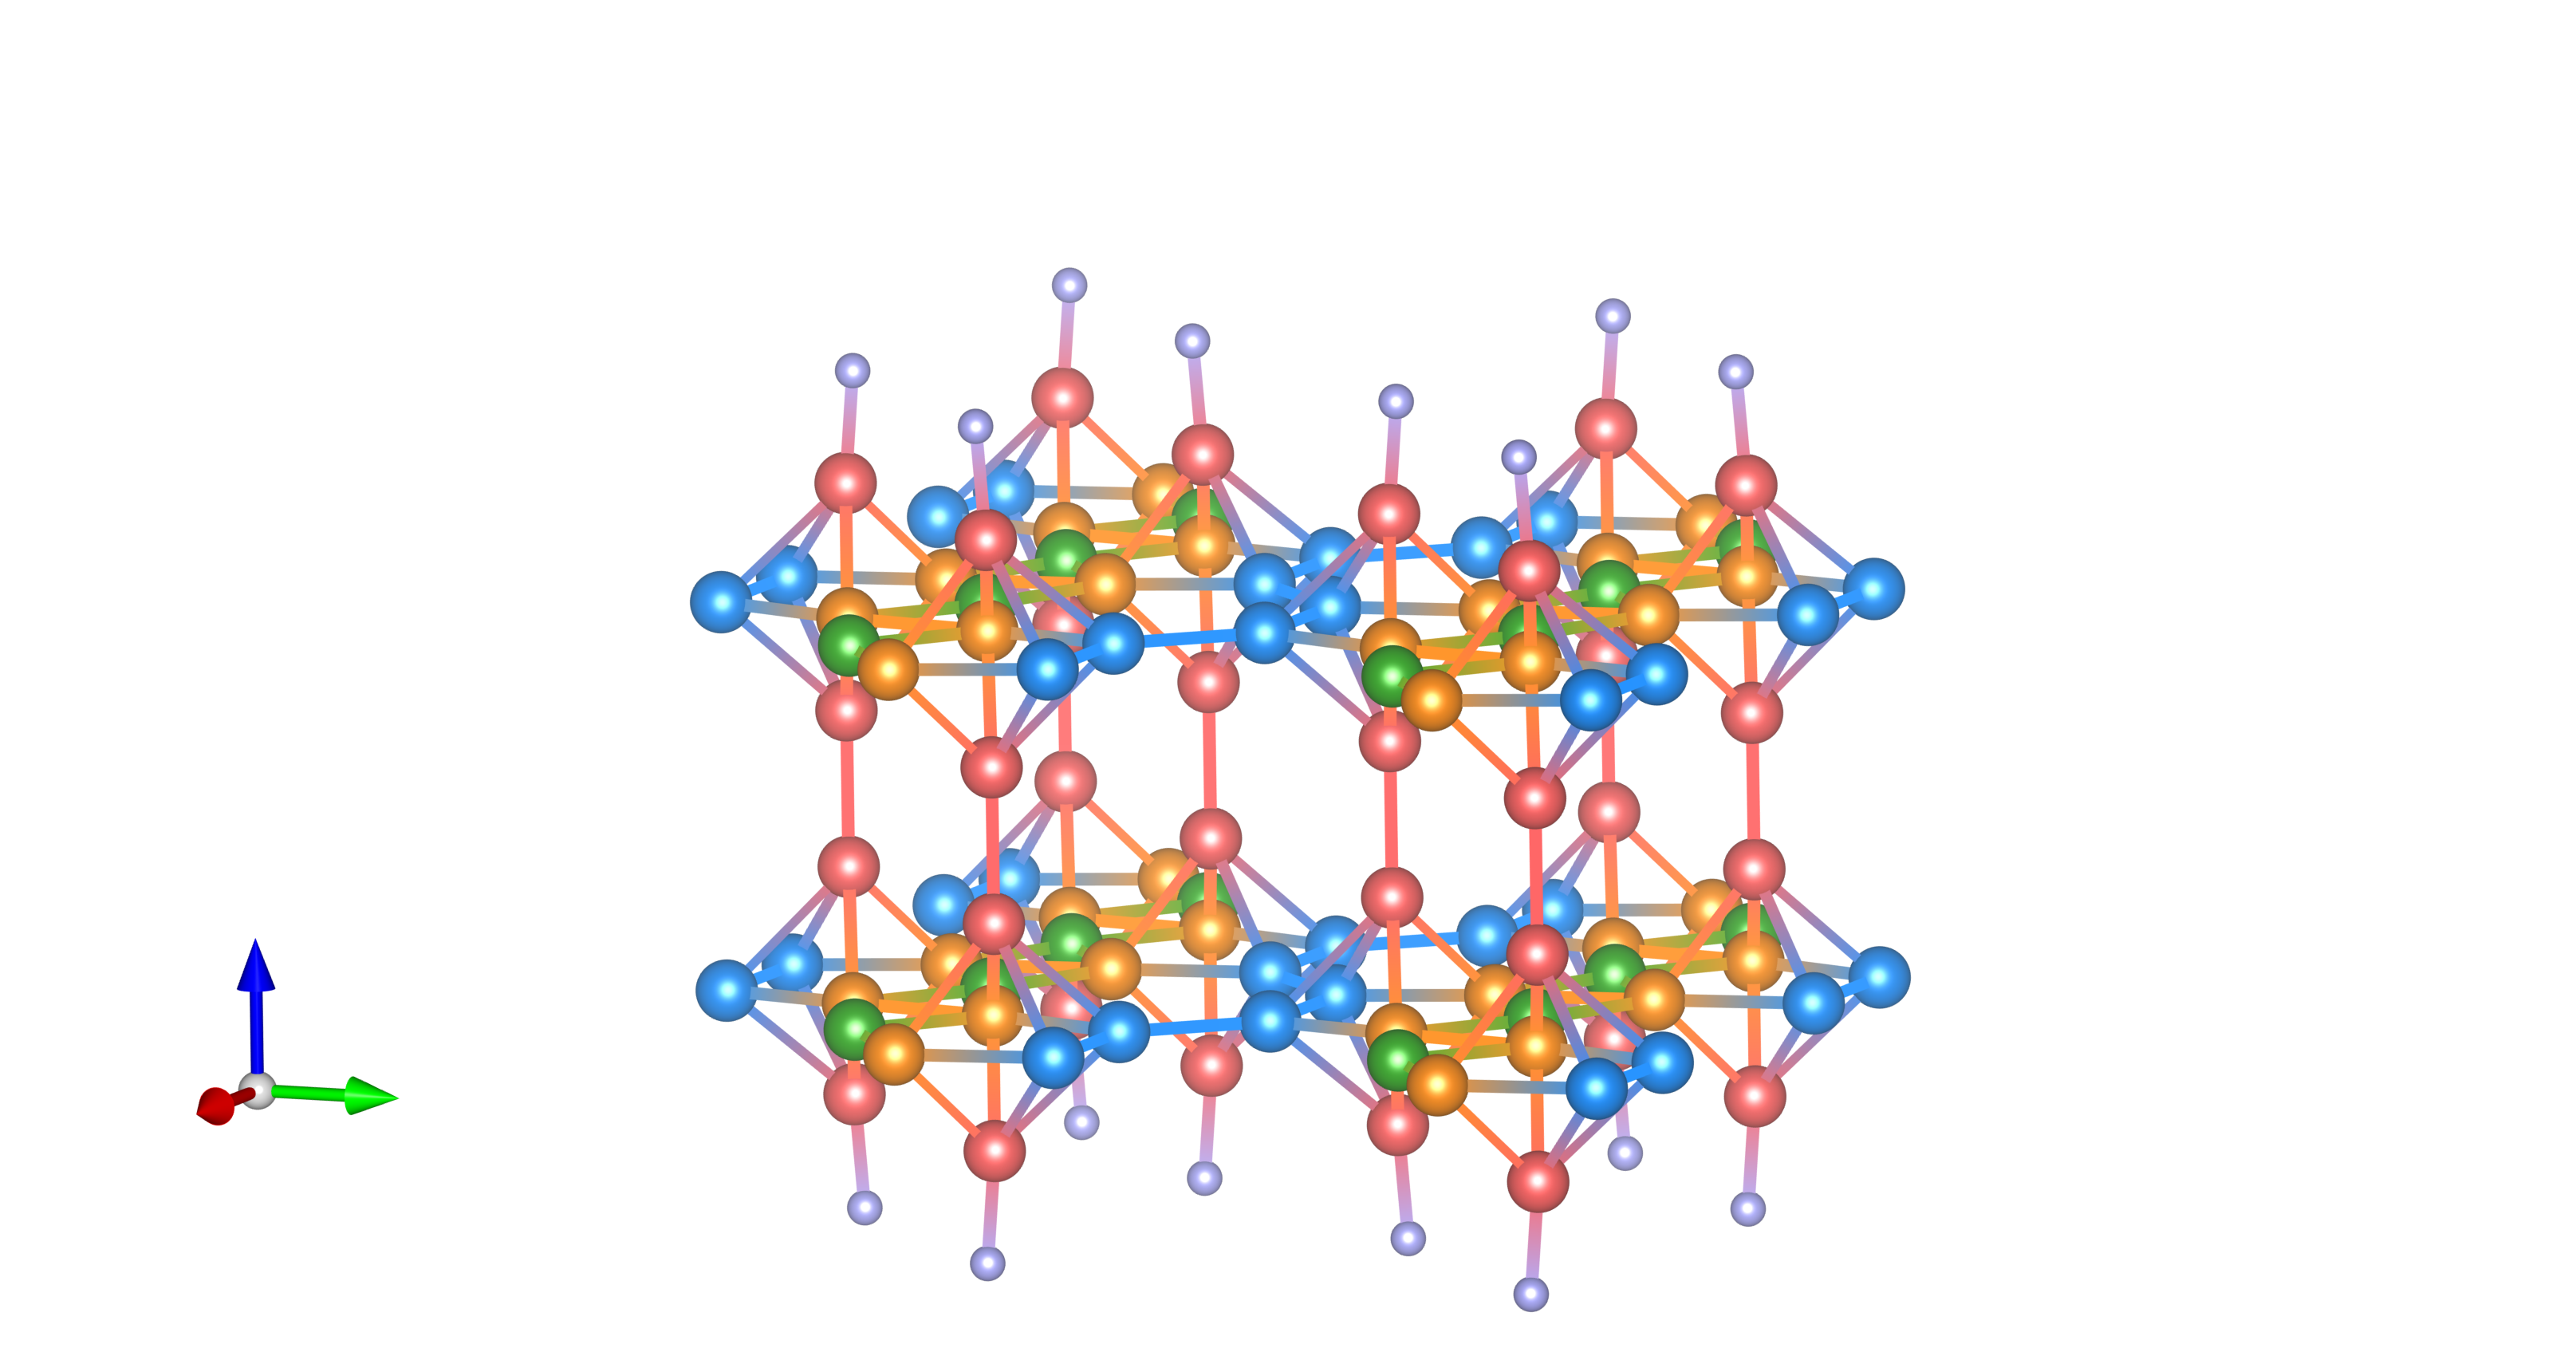
\includegraphics[width=0.8\linewidth]{figures_ch1/intro.png}
\caption{Atomic structure of hydrogen-terminated bilayer o-\ce{B14}. Large coloured spheres represent boron atoms, with different colours denoting crystallographically inequivalent boron sites. Small light-purple spheres represent hydrogen atoms. The figure illustrates a computational structural model considered in chapter~\ref{cha:project_boron}.}
\label{fig:intro}
\end{figure}

\FloatBarrier
\subsection{Beryllene and hydrogen functionalization}
\label{subsec:lit_beryllene}

The preceding discussion followed the effects of interfaces and surface bonding in boron-based systems.
We now consider beryllium, beginning with the geometry of the layer itself.
Ono compared ideal two-dimensional metals in several lattice arrangements using first-principles phonon calculations~\cite{ono2020dynamical}.
The resulting differences in dynamical stability show that a stable bulk element produces a stable sheet only in some geometries.
Hess examined periodic trends in two-dimensional bonding among main-group elements~\cite{hess2022periodicity}.
These studies guide the choice of candidate structures and relate their bonding to the atomic arrangement.
For each candidate, we also examine how the atoms respond to displacement.

Chahal et al. prepared beryllene sheets by sonochemical exfoliation of beryllium powder~\cite{chahal2023beryllene}.
Their microscopy revealed several lattice motifs, including hexagonal and square arrangements, and their transport measurements indicated metallic behaviour.
These observations establish an experimental basis for investigating thin beryllium structures.
To compare them with a calculation, we also need the layer number and the detailed atomic arrangement.
This requirement is especially relevant because different studies use the phase names $\alpha$ and $\beta$ for different structural descriptions.
We therefore identify each phase by its geometry as well as its name.

Li et al. investigated a triangular monolayer and a corresponding two-layer structure, which they denoted as $\alpha$- and $\beta$-beryllene, respectively~\cite{li2023coexistence}.
Their calculations identified non-trivial band topology in the $\alpha$ phase and a topologically trivial $\beta$ phase.
They also predicted superconductivity in both structures using electron-phonon and Migdal--Eliashberg calculations.
A subsequent preprint by Petrov and Milo\v{s}evi\'{c} reported weaker superconductivity in a reanalysis of these phases and questioned the temperature dependence of the superconducting gaps in the earlier calculation~\cite{petrov2024comment}.
To compare these quantitative predictions, we therefore need to examine the treatment of the pairing problem in each study, even for the same parent atomic structures.
We also distinguish the electronic band-topology analysis from the calculation of the superconducting state.

Layer number introduces a further structural variable.
Jiang et al. examined few-layer beryllene and found that the predicted superconductivity varied non-monotonically with layer number and stacking~\cite{jiang2025nonmonotonic}.
Their study related these changes to the electronic states and phonon-mediated coupling, and also examined non-trivial topology and interstitial electronic states.
Thus, the properties after adding a layer can deviate from a simple interpolation between the monolayer and the bulk.
The stacking arrangement changes both the interlayer bonding and the surface environment.
We therefore compare the geometries explicitly instead of classifying the structures only by layer number.

In chapter~\ref{cha:project_beryllene}, we extend the structural comparison to trilayer cubic beryllene and selected hydrogen-functionalized configurations.
Here, we use trilayer cubic beryllene to denote the ABA-stacked trilayer with a square lattice, distinguishing this geometry from other few-layer structures in the literature.
We examine the effect of the geometry and surface bonding on the electronic structure and optical response.
For the pristine and hydrogen-functionalized structures, we also investigate the band topology and explicitly state the required band-isolation conditions.
For trilayer cubic beryllene and the hydrogen-functionalized $\beta$-beryllene structures, we further calculate the electron-phonon coupling and the superconducting transition temperatures.

Let us next consider the hydrogen-beryllium bond.
Bachurin and Vladimirov studied hydrogen adsorption on beryllium surfaces using \textit{ab initio} calculations~\cite{bachurin2015ab}.
Such a surface retains the underlying bulk coordination, whereas both sides of a freestanding layer can respond to adsorption.
Li et al. instead used global structure search and first-principles calculations to propose two-dimensional beryllium hydride structures~\cite{li2018global}.
In that case, hydrogen enters the formation of a compound network.
These studies address related bonding questions in different structural environments.
In this thesis, we start from specified elemental layers and examine the changes introduced by selected hydrogen arrangements.
We determine the relaxed structure, compare its electronic character with that of the parent layer, and follow the resulting changes in the optical spectrum.

\subsection{Computational approaches and their limitations}
\label{subsec:lit_methods}

We have seen that previous studies use structural searches, electronic calculations, and response calculations to address different parts of the material problem.
We now connect these descriptions to the physical questions they address.
We develop the detailed theory and computational settings in the following chapters; here, we identify what each level of calculation contributes to the comparison.

Firstly, density functional theory (DFT) describes the electronic ground state and the forces acting on the atoms.
We employ semilocal approximations, such as the Perdew--Burke--Ernzerhof (PBE) functional, to relax structures and compare their energies~\cite{perdew1996generalized}.
Combining these calculations with a structural search, we can explore competing arrangements, as in the borophene and bulk o-\ce{B14} studies discussed above~\cite{penev2012polymorphism,han2023superconducting}.
After relaxing the geometry, we calculate the band structure to characterize the electronic states that enter the subsequent response calculations.

The exchange-correlation approximation enters this description directly.
Screened hybrid functionals include a fraction of short-range exact exchange and can modify the band separations and orbital ordering that a semilocal functional predicts~\cite{heyd2003hybrid,krukau2006influence}.
We use the 2006 form of the Heyd--Scuseria--Ernzerhof functional, denoted as HSE06, to compare selected results with PBE.
This comparison tests the sensitivity of the electronic and optical trends to the exchange-correlation treatment.
To describe quasiparticle excitations, the $GW$ approach approximates the electronic self-energy using the Green function and the screened Coulomb interaction.
The Bethe--Salpeter equation then incorporates the interaction between the excited electron and the hole~\cite{onida2002electronic}.
These distinctions are particularly relevant in two-dimensional systems, where screening depends strongly on the environment~\cite{thygesen2017}.
Our independent-particle optical calculations describe transitions within the adopted electronic structure.
They do not include the bound electron-hole excitations of a Bethe--Salpeter treatment.

Next, the electronic comparison requires a consistent structural reference.
In a heterostructure, we first determine the interlayer separation and atomic registry, then evaluate charge redistribution and band mixing at that geometry.
Dispersion corrections account for the van der Waals interactions missing from a semilocal functional and therefore enter the relaxation of the graphene-based bilayers~\cite{grimme2010consistent,grimme2011effect}.
We also specify how we represent the optical response.
A periodic calculation places a sheet and its surrounding vacuum in the same supercell.
Consequently, a dielectric quantity normalized to that cell depends on the vacuum spacing.
Matthes et al. discussed the relation between this response and that of an individual sheet or a film of specified thickness, including the out-of-plane response~\cite{matthes2016influence}.
We must account for this normalization when comparing optical magnitudes across different calculations or with a measurement.

We then turn to the motion of the atoms.
Structural relaxation locates a stationary configuration, while atomic displacements probe its stability.
Force constants, which we can calculate using density functional perturbation theory, determine the harmonic phonons that characterize the small-displacement response~\cite{baroni2001phonons}.
Ono, for example, used phonon calculations to compare two-dimensional metallic lattices~\cite{ono2020dynamical}.
\textit{Ab initio} molecular dynamics (AIMD) instead follows the atomic motion at a chosen temperature for a finite simulation time.
The two calculations therefore examine different aspects of the same structure: local harmonic stability and persistence during the simulated thermal motion.
Total-energy comparisons determine the energetic ordering of the chosen candidates.
We use these results together to assess a proposed model, while experimental formation also depends on competing phases, preparation pathways, and the environment.

Finally, we investigate phonon-mediated superconductivity through the coupling between electronic and lattice states.
Gao et al. used electron-phonon coupling in a McMillan--Allen--Dynes estimate of the transition temperature, whereas Li et al. treated the superconducting state of beryllene through Migdal--Eliashberg calculations~\cite{gao2017prediction,li2023coexistence}.
\texttt{EPW} employs Wannier interpolation to evaluate the relevant electron-phonon quantities on dense sampling meshes~\cite{ponce2016epw}.
The calculated transition temperature depends on this coupling and on the treatment of the pairing interaction.
Band topology requires a different extension of the electronic calculation: we must examine the wave functions over a suitable band subspace and use the symmetries of the system~\cite{fu2007topological}.
We return to its physical significance below.

\subsection{Experimental evidence and theoretical models}
\label{subsec:lit_critical_status}

We can now distinguish the experimental observations from the theoretical models that motivate this thesis.
Graphene, substrate-supported borophene, and epitaxial \ce{BC3} have experimental precedents, as do related borophene-graphene interfaces and exfoliated beryllium sheets~\cite{novoselov2004electric,mannix2015synthesis,feng2016experimental,tanaka2005novel,liu2019borophene,chahal2023beryllene}.
Our calculations describe specified freestanding geometries without the supporting surfaces or preparation environments of those experiments.
The \ce{B4C3} monolayer and bulk o-\ce{B14} framework instead originate from theoretical predictions~\cite{tian2019,han2023superconducting}.
We take these structures as references and investigate new interfaces or low-dimensional forms; the resulting properties remain predictions for those models.

This distinction also clarifies the comparison between the three projects.
For the graphene-based bilayers, we begin with selected monolayers and ask how their interaction changes the response.
For o-\ce{B14}, we begin with a predicted bulk network and change its dimensionality and surface termination.
For beryllium, we compare layer geometries and then modify their surface bonding.
In each case, we compare the modified structure with its reference and relate the changes in its calculated properties to the structural modification.

\section{Motivation for optical and topological analysis}
\label{sec:intro_observables}

% opening paragraph
So far, we have discussed how we select the atomic structures and calculate their electronic states.
We now examine what further information these states contain.
Optical response describes their interaction with an electromagnetic field.
Band topology characterizes how a selected set of wave functions connects across the Brillouin zone.
Both start from the electronic structure, but they answer different physical questions.

\subsection{Optical response as a probe of electronic structure}
\label{subsec:opt_observables_motivation}

The band structure specifies the electronic energies.
To describe the response to light, we also determine which transitions couple to the electric field and how strongly they do so.
A change in bonding can therefore modify an optical spectrum even when the material remains metallic or semiconducting.
Accordingly, we compare the optical properties together with the band structures of the isolated layers, heterostructures, and hydrogen-functionalized systems.

We first examine the energies and strengths of the interband transitions.
Within the independent-particle description, they determine the absorptive part of the dielectric response~\cite{onida2002electronic}.
We compare a monolayer with its heterostructure to trace how stacking redistributes this response over photon energy.
We then compare pristine and hydrogen-functionalized layers to examine how surface bonding modifies the spectrum.
The real part of the dielectric response describes the accompanying polarization and dispersion.
As we establish in chapter~\ref{cha:fundamentals_b}, causality connects these two parts, and we therefore examine them together.

We next resolve the response along different directions.
The in-plane and out-of-plane polarizations probe different electronic environments.
When the two in-plane directions are inequivalent, we also compare them to resolve the effect of structural anisotropy.
The dielectric tensor characterizes these directional responses within a common framework.
In the scalar treatment, the refractive index determines the phase propagation of light, whereas the extinction coefficient characterizes its attenuation.
The absorption coefficient quantifies the intensity decay per unit distance, and reflectivity specifies the fraction of incident intensity that returns from an interface under the assumed optical geometry.
These quantities therefore connect the dielectric response to the propagation, attenuation, and reflection of light.
Where we derive them from individual Cartesian diagonal components, we state that construction explicitly in the corresponding research chapter.
When off-diagonal components couple the response, we must solve the corresponding propagation problem to determine the optical modes.

We then consider the energy transferred by an external charged probe.
The energy-loss function depends on the screened response and can contain features associated with collective electronic motion~\cite{thygesen2017}.
A zero of the real dielectric function together with sufficiently weak damping can support a plasmon interpretation.
We therefore compare the energy-loss peaks with both parts of the dielectric response before assigning a mode.
For a two-dimensional sheet, momentum transfer, geometry, and the surrounding dielectric environment also enter the relation to electron energy-loss spectroscopy (EELS).
We use the calculated energy-loss spectra to trace changes in screening and examine possible collective excitations.

Finally, we retain the same conventions when comparing the spectra.
Metallic systems can have an intraband contribution at low frequency, while electron-hole interactions can change interband excitation energies and strengths~\cite{onida2002electronic}.
The treatment of these contributions, together with the vacuum or effective-thickness convention, determines what the calculation represents~\cite{matthes2016influence}.
The research chapters specify these choices for their respective systems.
With these choices specified, we relate the structural changes to the optical response and interpret its magnitude and spectral features within the corresponding approximations.

\subsection{Physical significance of band topology}
\label{subsec:topo_motivation}

We now turn from the response of the electronic states to their organization across the Brillouin zone.
This organization is specified by the wave functions, which contain information beyond the band energies.
For a two-dimensional insulating system with time-reversal symmetry and the appropriate spinful band description, a non-trivial $\mathbb{Z}_2$ index characterizes a phase with helical edge states~\cite{fu2007topological}.
Time reversal relates the counterpropagating states at an edge and restricts elastic backscattering between a Kramers pair as long as the system preserves that symmetry.
The index thus connects the bulk wave functions to boundary transport.
This connection also motivates us to investigate light-element materials, where weak spin-orbit coupling requires particular attention to the energy scales and band separations.

To evaluate the index, we first need a well-defined band subspace.
In an inversion-symmetric system, the Fu--Kane criterion uses the parity eigenvalues of its Kramers pairs at the time-reversal invariant momenta~\cite{fu2007topological}.
A direct gap must separate the selected subspace from the other bands throughout the Brillouin zone.
An indirect overlap can nevertheless make the material metallic, even when this direct gap is present.
We therefore distinguish the topology of an isolated subspace from an insulating state at the Fermi level.
To interpret the phase as a quantum spin Hall insulator, we also require an insulating bulk at the Fermi level.
Chapter~\ref{cha:fundamentals_c} develops these distinctions and the symmetry conditions in detail.
We then apply these conditions to the pristine and hydrogen-functionalized beryllium structures in chapter~\ref{cha:project_beryllene}.

\section{Research questions and scope of the thesis}
\label{sec:intro_gaps}

% opening paragraph
The preceding discussion leads to the common question of this thesis: how do changes in atomic structure modify the electronic structure and optical response of light-element two-dimensional materials?
We address this question through three comparisons, each beginning with a specified structural reference.
Starting from each reference, we form an interface, reduce the dimensionality, or modify the surface termination.

Firstly, we consider graphene coupled to borophene, \ce{BC3}, and \ce{B4C3}.
Earlier work establishes the relevance of these material families and shows that interlayer coupling can modify electronic states.
Here, we ask how stacking graphene with the selected metallic and semiconducting constituents modifies the electronic structure and polarization-dependent optical response.
We compare each bilayer with its isolated constituents within the same computational framework to identify the changes that accompany interface formation.

Next, we follow the pentagonal-bipyramid boron framework from the predicted bulk o-\ce{B14} structure to one- and two-layer forms, and then to hydrogen-terminated sheets.
The bulk prediction leaves open how reduced coordination and surface bonding affect this network.
We examine the resulting electronic and magnetic states, the electron-phonon properties, and the changes in optical response.
We compare the bulk, pristine sheets, and terminated sheets successively to distinguish the effects of dimensional reduction and hydrogen addition.

Finally, we examine the beryllium structures, extending the comparison of the $\alpha$ and $\beta$ phases to trilayer cubic beryllene and selected hydrogen-functionalized configurations.
We ask how the layer geometry and hydrogen arrangement affect structural stability, electronic states, electron-phonon coupling, and optical anisotropy.
For these structures, we also examine the band-topology interpretation and the separation of the relevant band subspaces.
These questions connect the structural comparison to the optical and topological considerations introduced above.

The three projects therefore follow the same physical sequence: a change in atomic arrangement modifies bonding and electronic states, which in turn changes the calculated response.
Magnetism, superconductivity, and topology enter where the particular electronic and lattice structure makes them relevant.
The conclusions concern the specified models and computational treatments.
We compare each modified structure with its reference to identify how structural modification changes the calculated properties and how these changes depend on the bonding environment.

\section{Thesis organization}
\label{sec:intro_organisation}

% opening paragraph
We first develop the theoretical descriptions needed for the material comparisons.
Chapter~\ref{cha:fundamentals_a} introduces the density-functional treatment of the many-body problem, the exchange-correlation approximations, and their use in practical calculations.
Chapter~\ref{cha:fundamentals_b} then develops the linear optical response, connecting the dielectric function to the optical quantities used later.
Chapter~\ref{cha:fundamentals_c} introduces the band-subspace and symmetry conditions for the topological analysis, including the distinction between a topological subspace and an insulating state at the Fermi level.

We then apply these descriptions to the three research projects.
Chapter~\ref{cha:project_bilayers} compares the graphene-based heterostructures with their constituent monolayers and examines how interfacial coupling modifies their electronic structure and optical response.
Chapter~\ref{cha:project_boron} follows dimensional reduction and hydrogen termination in the pentagonal-bipyramid boron framework, including the electronic, magnetic, electron-phonon, and optical properties.
Chapter~\ref{cha:project_beryllene} extends the discussion to pristine and hydrogen-functionalized beryllium structures, including trilayer cubic beryllene.
It examines their stability, electronic properties, band topology, electron-phonon coupling, and optical response.
Finally, chapter~\ref{cha:conclusion_outlook} integrates these findings and discusses the further questions that the results raise.

We develop the more general theoretical foundations in the appendices.
Appendix~\ref{cha:appendix_quantum} develops the quantum-mechanical background and the elementary density functionals.
Appendix~\ref{cha:appendix_electrodynamics} discusses the electromagnetic response and its causal structure.
Appendix~\ref{cha:appendix_topology} introduces geometric phases and the quantum-mechanical foundations of band topology.
Appendix~\ref{cha:appendix_code} describes the source code used in this thesis.

\cleardoublepage
\chapter[Fundamentals \textRoman{1}: From Many-Body Physics to DFT]{Fundamentals \textRoman{1}: From Many-body physics to Density Functional Theory}
\label{cha:fundamentals_a}

% opening paragraph
We start our discussion of the fundamentals in this chapter by introducing the many-body quantum framework underlying density functional theory.
The ionic structure creates an external potential, and the interacting electrons in this potential determine the electronic properties of the materials studied here.
In principle, the many-body wave function $\Psi$ contains the full electronic information of the system.
However, as $\Psi$ depends on all electronic coordinates, direct calculation becomes impractical for realistic materials.
We therefore proceed from the many-body wave function $\Psi$ to the electron density $n(\vec{r}\,)$, and then construct practical density functionals.

This chapter partly draws on my notes from the Coursera course \textit{Density Functional Theory}, offered by École Polytechnique and taught by Francesco Sottile and Lucia Reining~\cite{sottile_reining_dft_coursera}.

We develop this chapter as a gradual reduction of the electronic problem.
The many-body hamiltonian and the elementary functional definitions are given in appendix~\ref{cha:appendix_quantum}.
We start from density functionals in quantum mechanics and establish the Hohenberg--Kohn theorem in section~\ref{sec:introduction_density_functionals}.
With the electron density $n(\vec{r}\,)$ as the central variable, we construct the Kohn--Sham framework in section~\ref{sec:from_density_functional_to_Kohn_Sham_theory}.
Finally, section~\ref{sec:exchange_correlation_functional} demonstrates practical exchange-correlation approximations and brings the formal theory to the working form of density functional theory.

In section~\ref{sec:practical_computational_methods},
we then connect these foundations to the calculations used in this thesis.
Readers interested in the computational procedure can proceed directly to that section.
The supporting quantum-mechanical and Thomas--Fermi derivations are collected in appendix~\ref{cha:appendix_quantum}.

\newpage
\section{Density functional in quantum mechanics}
\label{sec:introduction_density_functionals}

In quantum mechanics, it is often convenient to shift the basic variable from the many-body wave function to the electron density $n(\vec{r}\,)$.
From this point of view, every relevant physical quantity can be expressed as a functional of the density.
Therefore, a functional takes the density $n(\vec{r}\,)$ as input and returns a quantum-mechanical observable as output.

We use the Hartree atomic units defined in subsection~\ref{sec:manybody_schrodinger_equation} of appendix~\ref{cha:appendix_quantum}:
$\hbar=1$, $m_\mathrm{e}=1$, $e=1$, and $4\mathrm{\pi}\varepsilon_0=1$.

To describe this process, we first introduce the density operator:

\begin{equation}
    \hat{n}(\vec{r}\,) = \sum_{i=1}^N \delta(\vec{r}-\hat{\vec{r}}_i\,)
\label{density_operator}
\end{equation}

Next, the expectation value of this operator in the ground state defines the ground-state electron density

\begin{equation}
    n(\vec{r}\,)\coloneqq\bra{\Psi_0}\hat{n}(\vec{r}\,)\ket{\Psi_0}
\label{electron_density_definition}
\end{equation}

here, $\ket{\Psi_0}$ denotes the ground-state many-body wave function, which encodes the full complexity of the current interacting $N$-electron system.
Given an observable represented by an operator $\hat{\Omega}$, its ground-state value is evaluated through the expectation value $\Omega$:

\begin{equation}
    \Omega \coloneqq \bra{\Psi_0}\hat{\Omega}\ket{\Psi_0}
\label{electron_density_expectation}
\end{equation}

and hence every ground-state observable can be regarded, at least formally, as a functional of the many-body wave function $\Omega[\Psi_0]=\Omega$.

However, the key idea of density functional theory is here.
For the ground-state properties, the wave function dependence can be reduced even further.
If the ground-state density $n(\vec{r}\,)$ uniquely specifies the corresponding ground-state wave function $\Psi_0$,
the expectation value of any operator $\hat{\Omega}$ in the ground state is uniquely determined by the density $n(\vec{r}\,)$.

Under the usual Hohenberg--Kohn setting (in particular, for a non-degenerate ground state), the density $n(\vec{r}\,)$ uniquely determines the external potential $v_\mathrm{ext}(\vec{r}\,)$ up to an additive constant.
Consequently, $n(\vec{r}\,)$ fixes the hamiltonian and hence the ground state $\ket{\Psi_0}$ (up to an overall phase).
This statement is essentially the central result of the Hohenberg--Kohn theorem~\cite{hohenberg1964inhomogeneous}, namely that in the ground state all observables are uniquely determined by the electron density.
Accordingly, any ground-state observable may be written as a functional of the density alone:

\begin{equation}
    \Omega = \Omega[n(\vec{r}\,)]
\label{ground_state_observable_density_functional}
\end{equation}

This relation marks the conceptual compression from a function of $3N$ variables, $\Psi_0(\vec{r}_1,\cdots,\vec{r}_N\,)$, to a function of only three spatial variables, $n(\vec{r}\,)$, which is the cornerstone of the practical formulation of DFT.
Historically, the density-functional formalism was established in the 1960s through the pioneering work of Hohenberg and Kohn, and was later made computationally practical by the Kohn--Sham scheme~\cite{kohn1965self}.

Since the many-body wave function $\Psi$ encodes the full complexity of the system, a natural question is the following: what is the ingredient that actually distinguishes one many-electron system from another?

To answer this, we recall that the quantum dynamics is specified once the hamiltonian is given.

For electronic systems, the kinetic energy operator $\hat{T}=\hat{T}_\mathrm{e}$ and the interaction operator $\hat{V}_\mathrm{int}=\hat{V}_\mathrm{ee}$ have the fixed forms given in equations~\eqref{electrons_kinetic} and~\eqref{electrons_Coulomb}.

Therefore, the system-specific information enters primarily through the external potential $\hat{V}_\mathrm{ext}$, which is generated by the nuclei and any applied fields.
With this in mind, we review the form of hamiltonian:

\begin{equation}
    \hat{H}=\hat{T}+\hat{V}_\mathrm{int}+\hat{V}_\mathrm{ext}
\label{hamiltonian_decomposition}
\end{equation}

In subsection~\ref{sec:manybody_schrodinger_equation} of appendix~\ref{cha:appendix_quantum},
we discuss in detail the explicit forms and physical meanings of the kinetic, external potential, and interaction terms in the many-body hamiltonian.

Let us return to the reduced expression for the hamiltonian in equation~\eqref{clamped_nuclei_many_body_hamiltonian}.
We observe that two terms are universal, in the sense that their operator forms do not depend on the specific system.

These are the electronic kinetic energy~\eqref{electrons_kinetic},
and the electron-electron Coulomb repulsion~\eqref{electrons_Coulomb}.

Here, we say the external potential $\hat{V}_\mathrm{ext}$ is not universal, because it depends on the specific nuclear configuration and any applied fields. In contrast, the electronic kinetic energy and the electron-electron Coulomb interaction have fixed operator forms.
Therefore, the external potential is the system-defining ingredient: it distinguishes one many-electron system from another.

In fact, once $\hat{V}_\mathrm{ext}$ is given, the hamiltonian is fully specified.
Conversely, if the hamiltonian is known, then in principle we may solve its eigenvalue problem to obtain the eigenstates and eigenvalues.
With the wave function known, any observable can be evaluated as the expectation value of the corresponding operator.

This viewpoint motivates the search for compact descriptors that retain the essential information of the ground state.
A central example is the electron density.
For an arbitrary state $\ket{\Psi}$, the electron density is defined as the expectation value of the density operator $\hat{n}(\vec{r}\,)$:

\begin{equation}
\begin{aligned}
   n(\vec{r}\,)&=\bra{\Psi}\hat{n}(\vec{r}\,)\ket{\Psi} \\
   &=\bra{\Psi}\sum_i \delta(\vec{r}-\hat{\vec{r}}_i\,)\ket{\Psi}
\end{aligned}
\label{electron_densit_via_expectation}
\end{equation}

For a fixed form of interaction, the external potential $v_\mathrm{ext}(\vec{r}\,)$ specifies the corresponding hamiltonian and therefore the ground-state structure.
Here $v_\mathrm{ext}(\vec{r}\,)$ is a scalar potential field in real space, whereas $\hat{V}_\mathrm{ext}$ is the associated many-body operator acting on the $N$-electron wave function.

Given the definition of the external potential operator~\eqref{Electron-nucleus_one-body_form}, in coordinate representation, $\hat{V}_\mathrm{ext}$ acts by multiplication with $\sum_i v_\mathrm{ext}(\hat{\vec{r}}_i\,)$.

For later convenience, we use the particle-density operator in equation~\eqref{density_operator} to express the external potential operator.
Since $v_\mathrm{ext}(\vec{r}\,)$ then couples locally to the density operator $\hat{n}(\vec{r}\,)$, we obtain:

\begin{equation}
    \hat{V}_\mathrm{ext}=\int\mathrm{d}\vec{r}\,v_\mathrm{ext}(\vec{r}\,)\,\hat{n}(\vec{r}\,)
\label{local_external_potential_operator_definition}
\end{equation}

Taking the expectation value on an arbitrary state $\ket{\Psi}$ yields the corresponding external potential energy. Using the expectation value of the density operator as in
equation~\eqref{electron_densit_via_expectation}, we have:

\begin{equation}
    \braket{\hat{V}_\mathrm{ext}}=\int\mathrm{d}\vec{r}\,v_\mathrm{ext}(\vec{r}\,)\,n(\vec{r}\,)
\label{external_potential_energy_expectation}
\end{equation}

When the ground state is non-degenerate, $v_\mathrm{ext}(\vec{r}\,)$ stands in a one-to-one correspondence (up to an additive constant) with the ground-state wave function $\Psi_0$.

Consequently, the ground-state expectation value of any observable $\hat{\Omega}$ may be viewed as a unique functional of the external potential:

\begin{equation}
   \braket{\hat{\Omega}}\coloneqq \bra{\Psi_0}\hat{\Omega}\ket{\Psi_0}=\Omega[v_\mathrm{ext}]
\label{functional_from_external_potential}
\end{equation}

The central move of density functional theory is to further replace the dependence on the wave function by a dependence on the electron density $n(\vec{r}\,)$.
The key question is whether the map from external potential $v_\mathrm{ext}(\vec{r}\,)$ to the ground-state density $n(\vec{r}\,)$ is likewise invertible in an appropriate sense.
The first Hohenberg--Kohn theorem answers this in the affirmative for non-degenerate ground states: the ground-state density $n(\vec{r}\,)$ uniquely determines $v_\mathrm{ext}(\vec{r}\,)$ (again up to an additive constant), and hence uniquely fixes the hamiltonian and the corresponding ground state.
In this sense, all ground-state observables can be regarded as functionals of the density.

In the presence of ground-state degeneracy, the strict one-to-one correspondence must be understood at the level of the ground-state subspace; certain observables may then depend on the particular choice of degenerate ground state. This issue is commonly handled through an ensemble formulation (or via a symmetry-breaking limit) to recover a single-valued density-functional description.

\subsection{The Hohenberg--Kohn theorem}

In this subsection, we focus on the Hohenberg--Kohn theorem, which provides the conceptual foundation of density functional theory: for a fixed form of electron-electron interaction and a non-degenerate ground state, it establishes a one-to-one correspondence between the external potential and the ground-state density (up to an additive constant), and it leads to a variational characterization of the ground state.

We start by assuming for contradiction that two different external potentials lead to the same ground-state wave function $\ket{\Psi_0}$, while not differing by a mere additive constant:

\begin{equation}
    v^{(1)}_\mathrm{ext}(\vec{r}\,)\neq v^{(2)}_\mathrm{ext}(\vec{r}\,)+\mathrm{const.}
\label{V_ext}
\end{equation}

Next, consider the corresponding hamiltonians and their ground-state eigenvalue equations:

\begin{equation}
\begin{aligned}
    \hat{H}_1=\hat{T}+\hat{V}_\mathrm{int}+\hat{V}_\mathrm{ext}^{(1)} &\implies \hat{H}_1\ket{\Psi_0^{(1)}}=E_1\ket{\Psi_0^{(1)}} \\
    \hat{H}_2=\hat{T}+\hat{V}_\mathrm{int}+\hat{V}_\mathrm{ext}^{(2)} &\implies \hat{H}_2\ket{\Psi_0^{(2)}}=E_2\ket{\Psi_0^{(2)}}
\end{aligned}
\label{different_hamiltonians_schrodinger_equation}
\end{equation}

Subtracting the two equations yields:

\begin{equation}
    (\hat{H}_1-\hat{H}_2)\ket{\Psi_0}=(E_1-E_2)\ket{\Psi_0}
\label{difference_eigen}
\end{equation}

Review the expression for the external potential operator in equation~\eqref{Electron-nucleus_one-body_form}.
Since $\hat{T}$ and $\hat{V}_\mathrm{int}$ are identical in $\hat{H}_1$ and $\hat{H}_2$, the difference comes entirely from the external potential term.
Therefore, for an $N$-electron system, we have:

\begin{equation}
\begin{aligned}
    \sum_{i=1}^N\left[v_\mathrm{ext}^{(1)}(\vec{r}_i\,)-v_\mathrm{ext}^{(2)}(\vec{r}_i\,)\right]\ket{\Psi_0}
    &= (\hat{V}_\mathrm{ext}^{(1)}-\hat{V}_\mathrm{ext}^{(2)})\ket{\Psi_0} \\
    &= (E_1-E_2)\ket{\Psi_0}
\end{aligned}
\label{energy_difference}
\end{equation}

Whenever the wave function $\Psi_0(\vec{r}_1,\vec{r}_2,\cdots,\vec{r}_N\,)\neq 0$, we can divide both sides by $\Psi_0$ and obtain:

\begin{equation}
    \sum_{i=1}^N\left[v_\mathrm{ext}^{(1)}(\vec{r}_i\,)-v_\mathrm{ext}^{(2)}(\vec{r}_i\,)\right]=E_1-E_2
\label{difference_energy_nowave}
\end{equation}

The equality above implies that, for any configuration $(\vec{r}_1,\vec{r}_2,\cdots,\vec{r}_N\,)$ where the wave function $\Psi_0(\vec{r}_1,\vec{r}_2,\cdots,\vec{r}_N\,)\neq 0$, the factor multiplying $\Psi_0$ must be constant.
Dividing both sides by $\Psi_0$ wherever the ground-state wave function $\Psi_0(\vec{r}_1,\ldots,\vec{r}_N\,)$ is non-zero, we obtain a constraint on the difference between the two external potentials.

To make this explicit, we define the potential shift function:

\begin{equation}
    g(\vec{r}\,)\coloneqq v_\mathrm{ext}^{(1)}(\vec{r}\,)-v_\mathrm{ext}^{(2)}(\vec{r}\,)
\label{shift_potential}
\end{equation}

Then, we can rewrite the previous relation as:

\begin{equation}
    g(\vec{r}_1\,)+g(\vec{r}_2\,)+\cdots+g(\vec{r}_N\,)=E_1-E_2
\label{N-body_shift_potential}
\end{equation}

for all configurations on which the wave function $\Psi_0(\vec{r}_1,\vec{r}_2,\cdots,\vec{r}_N\,)$ is non-zero.

Now, we pick any set of coordinates $(\vec{r}_2,\cdots,\vec{r}_N\,)$ such that the wave function does not vanish, and keep them fixed.
With these coordinates held fixed, the sum of the last $N-1$ terms,
$g(\vec{r}_2\,)+\cdots+g(\vec{r}_N\,)$, is just a scalar.
The equation then reduces to:

\begin{equation}
    g(\vec{r}_1\,)= (E_1-E_2)-\left[g(\vec{r}_2\,)+\cdots+g(\vec{r}_N\,)\right]
\label{fixed_N-body_shift_potential}
\end{equation}

which shows that $g(\vec{r}_1\,)$ cannot change as $\vec{r}_1$ varies within any region where the wave function remains non-zero.
Otherwise the left-hand side would vary with $\vec{r}_1$, while the right-hand side remains fixed.

Since the same argument applies when we vary any other particle coordinate $\vec{r}_j$ with the remaining coordinates fixed,
we conclude that $g(\vec{r}\,)$ must be a constant almost everywhere on the set where $\Psi_0(\vec{r}_1,\ldots,\vec{r}_N\,)$ is non-zero.
Thus, we arrive at the following relation:

\begin{equation}
    v_\mathrm{ext}^{(1)}(\vec{r}\,)=v_\mathrm{ext}^{(2)}(\vec{r}\,)+\mathrm{const.}
\label{parallel_wave_function}
\end{equation}

Hence $g(\vec{r}\,)=(E_1-E_2)/N$, which contradicts the assumption in equation~\eqref{V_ext}.
Therefore, we arrive at the conclusion that two different external potentials cannot lead to the same non-degenerate ground-state wave function unless they differ only by an additive constant, as stated in equation~\eqref{parallel_wave_function}.

Equivalently, up to a constant shift in the potential and for a fixed form of interaction, the mapping from the external potential to the non-degenerate ground-state wave function is one-to-one.

Since any ground-state observable follows uniquely from the ground-state wave function via its expectation value, equation~\eqref{functional_from_external_potential} implies that $\ket{\Psi_0}$ is uniquely determined by $v_\mathrm{ext}$, and hence the ground-state observables are unique functionals of $v_\mathrm{ext}$.
The external potential is defined to an additive constant shift.

A natural question then is: what is the relation between the external potential $v_\mathrm{ext}(\vec{r}\,)$ and the density of the current system $n(\vec{r}\,)$?

To state this more precisely, we next define the equivalence class of external potential $v_\mathrm{ext}(\vec{r}\,)$ and the ground-state wave function $\ket{\Psi_0}$ as:

\begin{equation}
\begin{aligned}
    \left[v_\mathrm{ext}\right]&\coloneqq\left\{ v_\mathrm{ext}(\vec{r}\,) +\mathrm{const.}\right\}\\
    \left[\ket{\Psi_0}\right]&\coloneqq\left\{\mathrm{e}^{\mathrm{i}\theta}\ket{\Psi_0} \,\middle|\,\theta\in\mathbb{R}\right\}
\end{aligned}
\label{equivalence_classes_definition}
\end{equation}

To address this question, we fix the form of interaction and restrict ourselves to a non-degenerate ground state.
Under these assumptions, there is a one-to-one correspondence between the equivalence class of external potential $\left[v_\mathrm{ext}(\vec{r}\,)\right]$ and the ground-state wave function $\left[\ket{\Psi_0}\right]$, 
where $\left[v_\mathrm{ext}(\vec{r}\,)\right]$ is defined up to an additive constant and $\left[\ket{\Psi_0}\right]$ up to an overall phase.

Equivalently, $\left[v_\mathrm{ext}(\vec{r}\,)\right]$ and $\left[\ket{\Psi_0}\right]$ are in bijection:

\begin{equation}
    \left[v_\mathrm{ext}(\vec{r}\,)\right]\,\longleftrightarrow\,\left[\ket{\Psi_0}\right]
\label{potential_wave_function_correspondence}
\end{equation}

Moreover, the wave function is directly related to the density through the standard marginalization over the remaining $N-1$ particles. As a result, we obtain a unique ground-state density, given by the usual marginalization of the squared modulus of the wave function over all but one space variables:

\begin{equation}
    n(\vec{r}\,)=N\int \mathrm{d}\vec{r}_2\cdots\mathrm{d}\vec{r}_N\,\left|\Psi(\vec{r},\vec{r}_2,\cdots,\vec{r}_N\,)\right|^2
\label{density_function}
\end{equation}

here, $\Psi$ is normalized and $N$ is the number of particles.
This means that the external potential $v_\mathrm{ext}$ induces a mapping to the ground-state density $n(\vec r\,)$.
This subsection further clarifies the character of this mapping.

The strategy to establish this relation is also a reductio ad absurdum argument.
Suppose there exist two different external potentials $v^{(1)}_\mathrm{ext}(\vec{r}\,)$ and $v^{(2)}_\mathrm{ext}(\vec{r}\,)$ such that $v^{(1)}_\mathrm{ext}(\vec{r}\,)\neq v^{(2)}_\mathrm{ext}(\vec{r}\,)+\mathrm{const.}$
Let their corresponding non-degenerate ground-state wave functions be denoted as $\Psi_0^{(1)}$ and $\Psi_0^{(2)}$.

Recall the Schrödinger equation~\eqref{different_hamiltonians_schrodinger_equation}.
The external potentials $v^{(1)}_\mathrm{ext}(\vec{r}\,)$ and $v^{(2)}_\mathrm{ext}(\vec{r}\,)$ lead to the eigenvalues $E_1$ and $E_2$, and the corresponding ground-state wave functions $\ket{\Psi_0^{(1)}}$ and $\ket{\Psi_0^{(2)}}$, respectively.
The first part of the proof, summarized in equation~\eqref{parallel_wave_function}, excludes a common non-degenerate ground state for these two potentials.
Therefore, the two ground states differ, $\ket{\Psi_0^{(1)}}\neq\ket{\Psi_0^{(2)}}$.
For each external potential, the total energy can be written as the expectation value of the hamiltonian in its ground state:

\begin{equation}
\begin{aligned}
    E_1 &= \bra{\Psi_0^{(1)}}\hat{H}_1\ket{\Psi_0^{(1)}} \\
    E_2 &= \bra{\Psi_0^{(2)}}\hat{H}_2\ket{\Psi_0^{(2)}}
\end{aligned}
\label{different_total_energies}
\end{equation}

We now make the key assumption for contradiction: although the two external potentials, and hence the two ground-state wave functions, are different, they lead to the same ground-state density $n^{(1)}(\vec{r}\,)=n^{(2)}(\vec{r}\,)$, where $n^{(1)}(\vec{r}\,)$ and $n^{(2)}(\vec{r}\,)$ are obtained from $\Psi_0^{(1)}$ and $\Psi_0^{(2)}$, respectively, via equation~\eqref{density_function}.

According to the Rayleigh--Ritz variational principle, the energy expectation value over any normalized trial wave function $\Phi$ provides an upper bound to the ground-state energy $E_0$ of a given hamiltonian $\hat{H}$:

\begin{equation}
    E_0\leq \bra{\Phi}\hat{H}\ket{\Phi}
\label{Rayleigh-Ritz_principle}
\end{equation}

Therefore, using $\ket{\Psi_0^{(2)}}$ as a trial state for $\hat{H}_1$ and using $\ket{\Psi_0^{(1)}}$ as a trial state for $\hat{H}_2$, we obtain:

\begin{equation}
\begin{aligned}
    E_1&=\bra{\Psi_0^{(1)}}\hat{H}_1\ket{\Psi_0^{(1)}}<\bra{\Psi_0^{(2)}}\hat{H}_1\ket{\Psi_0^{(2)}}\\
    E_2&=\bra{\Psi_0^{(2)}}\hat{H}_2\ket{\Psi_0^{(2)}}<\bra{\Psi_0^{(1)}}\hat{H}_2\ket{\Psi_0^{(1)}}
\end{aligned}
\label{Rayleigh-Ritz_principle_application}
\end{equation}

here, the strict inequalities follow from the assumption that the ground state is non-degenerate and that $\ket{\Psi_0^{(1)}}\neq\ket{\Psi_0^{(2)}}$.

Let us rewrite the variational bound for $E_1$.
Recall the eigenvalue equation~\eqref{difference_eigen} and the definition of the hamiltonian difference in equation~\eqref{energy_difference}.
We can  expand the right-hand side as:

\begin{equation}
\begin{aligned}
    E_1=\bra{\Psi_0^{(1)}}\hat{H}_1\ket{\Psi_0^{(1)}}<\bra{\Psi_0^{(2)}}\hat{H}_1\ket{\Psi_0^{(2)}}
    &=\bra{\Psi_0^{(2)}}(\hat{H}_1-\hat{H}_2+\hat{H}_2)\ket{\Psi_0^{(2)}} \\
    &=\bra{\Psi_0^{(2)}}\hat{H}_2\ket{\Psi_0^{(2)}}
      +\bra{\Psi_0^{(2)}}(\hat{H}_1-\hat{H}_2)\ket{\Psi_0^{(2)}} \\
    &=E_2+\bra{\Psi_0^{(2)}}(\hat{V}_\mathrm{ext}^{(1)}-\hat{V}_\mathrm{ext}^{(2)})\ket{\Psi_0^{(2)}}
\end{aligned}
\label{H1_expectation_expansion}
\end{equation}

The further step is to rewrite the last term in a density form.
Let us apply the definition of the electron-density function~\eqref{electron_densit_via_expectation} as:

\begin{equation}
    n^{(2)}(\vec{r}\,) = \bra{\Psi_0^{(2)}}\hat{n}(\vec{r}\,)\ket{\Psi_0^{(2)}}
\label{density_expectation_definition}
\end{equation}

Then, we apply the definition of the operator for external potential~\eqref{local_external_potential_operator_definition}, and obtain:

\begin{equation}
\begin{aligned}
    \bra{\Psi_0^{(2)}}(\hat{V}_\mathrm{ext}^{(1)}-\hat{V}_\mathrm{ext}^{(2)})\ket{\Psi_0^{(2)}}
    &=\int \mathrm{d}\vec{r}\,\left[v_\mathrm{ext}^{(1)}(\vec{r}\,)-v_\mathrm{ext}^{(2)}(\vec{r}\,)\right]\,\bra{\Psi_0^{(2)}}\hat{n}(\vec{r}\,)\ket{\Psi_0^{(2)}} \\
    &=\int \mathrm{d}\vec{r}\,\left[v_\mathrm{ext}^{(1)}(\vec{r}\,)-v_\mathrm{ext}^{(2)}(\vec{r}\,)\right]\,n^{(2)}(\vec{r}\,)
\end{aligned}
\label{density_form_vext_difference}
\end{equation}

As a result, the total energy of the first system satisfies the following inequality:
\begin{equation}
    E_1<E_2+\bra{\Psi_0^{(2)}}\left(\hat{V}_\mathrm{ext}^{(1)}-\hat{V}_\mathrm{ext}^{(2)}\right)\ket{\Psi_0^{(2)}}
\end{equation}

Therefore, we arrive at the following inequality for the ground-state energies:

\begin{equation}
    E_1<E_2+\int \mathrm{d}\vec{r}\,\left[v_\mathrm{ext}^{(1)}(\vec{r}\,)-v_\mathrm{ext}^{(2)}(\vec{r}\,)\right]\,\,n^{(2)}(\vec{r}\,)
\label{total_energy_inequality_E1}
\end{equation}

Vice versa, upon interchanging the roles of the two systems, we analogously obtain:

\begin{equation}
    E_2<E_1+\int \mathrm{d}\vec{r}\,\left[v_\mathrm{ext}^{(2)}(\vec{r}\,)-v_\mathrm{ext}^{(1)}(\vec{r}\,)\right]\,\,n^{(1)}(\vec{r}\,)
\label{total_energy_inequality_E2}
\end{equation}

We are now ready to complete the reductio ad absurdum argument.
Under our assumption that two distinct external potentials $v_\mathrm{ext}^{(1)}(\vec{r}\,)\neq v_\mathrm{ext}^{(2)}(\vec{r}\,)$ yield the same ground-state density $n(\vec{r}\,)=n^{(1)}(\vec{r}\,)=n^{(2)}(\vec{r}\,)$, the Rayleigh--Ritz variational principle leads to the previous ground-state energy inequalities.

Using $n(\vec{r}\,)=n^{(1)}(\vec{r}\,) = n^{(2)}(\vec{r}\,)$ and adding equations~\eqref{total_energy_inequality_E1}
and~\eqref{total_energy_inequality_E2}, the integral terms cancel identically, which leads to:

\begin{equation}
    E_1 + E_2 < E_1 + E_2
\label{total_energy_inequality_contradiction}
\end{equation}

It is obviously a contradiction.
This demonstrates that, for a fixed form of interaction and a non-degenerate ground state,
the ground-state density $n(\vec{r}\,)$ uniquely determines the external potential $v_\mathrm{ext}(\vec{r}\,)$ up to an additive constant,
and hence uniquely determines the hamiltonian and the ground state up to an overall phase.

Let us recollect the definition of the equivalence class of the external potential $v_\mathrm{ext}(\vec{r}\,)$ and the ground-state wave function $\ket{\Psi_0}$ in equation~\eqref{equivalence_classes_definition},
as well as the fact that the equivalence classes $\left[v_\mathrm{ext}\right]$ and $\left[\ket{\Psi_0}\right]$ are in bijection in equation~\eqref{potential_wave_function_correspondence}.

Moreover, the ground-state wave function uniquely determines the ground-state density via the standard marginalization:

\begin{equation}
    \left[\ket{\Psi_0}\right]\longmapsto n(\vec{r}\,)
\label{wave_function_density_map}
\end{equation}

We emphasize that the map in equation~\eqref{wave_function_density_map} is not injective for any arbitrary many-body wave function.
In the present setting, however, we restrict ourselves to non-degenerate ground states. Within this restricted class, the first Hohenberg--Kohn theorem provides a unique inverse implication, namely that the ground-state density uniquely determines the equivalence class of the external potential:

\begin{equation}
    n(\vec{r}\,)\longmapsto\left[v_\mathrm{ext}(\vec{r}\,)\right]
\label{density_potential_map}
\end{equation}

Combining equations~\eqref{potential_wave_function_correspondence}, \eqref{wave_function_density_map},
and~\eqref{density_potential_map}, we finally arrive at a one-to-one correspondence among the basic ground-state descriptors:

\begin{equation}
    \left[v_\mathrm{ext}(\vec{r}\,)\right]\,\longleftrightarrow\, n(\vec{r}\,)\,\longleftrightarrow\,\left[\ket{\Psi_0}\right]
\label{hk_correspondence_v_n_psi}
\end{equation}

The two previous equations~\eqref{density_potential_map} and~\eqref{hk_correspondence_v_n_psi} summarize the content of the Hohenberg--Kohn theorem~\cite{hohenberg1964inhomogeneous,burke2012perspective}.
For a fixed form of interaction and a non-degenerate ground state, the ground-state density $n(\vec{r}\,)$ is in bijection with the equivalence class of the external potential $\left[v_\mathrm{ext}(\vec{r}\,)\right]$ up to an additive constant. 
Consequently, the ground-state density uniquely determines the hamiltonian and the ground-state wave function up to an overall phase,
and any ground-state observable is, in principle, a unique functional of $n(\vec{r}\,)$.

Therefore, the ground-state expectation definition~\eqref{functional_from_external_potential} can be reformulated as:

\begin{equation}
   \braket{\hat{\Omega}}= \bra{\Psi_0}\hat{\Omega}\ket{\Psi_0}=\Omega[n(\vec{r}\,)]
\label{functional_from_density}
\end{equation}

here, $\Omega[n(\vec{r}\,)]$ denotes the density functional that yields the ground-state expectation value of $\hat{\Omega}$.
This observation forms the central premise of density functional theory and motivates the use of the density, rather than the wave function, as the fundamental variable.

The ground-state energy is the expectation value of the hamiltonian in its ground state.
According to the decomposition of the hamiltonian in equation~\eqref{hamiltonian_decomposition}, we write:

\begin{equation}
\begin{aligned}
    E_0
    &= \bra{\Psi_0}\hat{H}\ket{\Psi_0} \\
    &= \bra{\Psi_0}(\hat{T}+\hat{V}_\mathrm{int}+\hat{V}_\mathrm{ext})\ket{\Psi_0}
\end{aligned}
\label{groundstate_energy_decomposition}
\end{equation}

To generalize this variational picture, for a given admissible density $n(\vec{r}\,)$ we consider wave functions $\Psi$ that yield $n$, and define:

\begin{equation}
\begin{aligned}
    E[n]
    &= \min_{\Psi\to n}\bra{\Psi}(\hat{T}+\hat{V}_\mathrm{int}+\hat{V}_\mathrm{ext})\ket{\Psi} \\
    &= \bra{\Psi[n]}(\hat{T}+\hat{V}_\mathrm{int}+\hat{V}_\mathrm{ext})\ket{\Psi[n]}
\end{aligned}
\label{functional_energy_constrained_search}
\end{equation}

which reduces to $E_0$ when $n=n_0$.

Here the minimization is taken over all normalized antisymmetric $N$-electron wave functions $\ket{\Psi}$ compatible with the fixed interaction.

The kinetic energy functional $K[n]$, the interaction energy functional $E_\mathrm{int}[n]$, and the external potential energy functional $E_\mathrm{ext}[n]$ are evaluated on a minimizing wave function $\Psi[n]$ that yields the density $n$.
We use $K$ for kinetic energy and $T$ for temperature.
We now write their definitions:

\begin{equation}
\begin{aligned}
    K[n]&\coloneqq\bra{\Psi[n]}\hat{T}\ket{\Psi[n]} \\
    E_\mathrm{int}[n]&\coloneqq\bra{\Psi[n]}\hat{V}_\mathrm{int}\ket{\Psi[n]} \\
    E_\mathrm{ext}[n]&\coloneqq\bra{\Psi[n]}\hat{V}_\mathrm{ext}\ket{\Psi[n]}
\end{aligned}
\label{functional_T_Eint_Eext_definition}
\end{equation}

Using the local form of the external potential operator in equation~\eqref{local_external_potential_operator_definition}, we get the local form of the external potential energy functional:

\begin{equation}
    E_\mathrm{ext}[n]=\int\mathrm{d}\vec{r}\,v_\mathrm{ext}(\vec{r}\,)\,n(\vec{r}\,)
\label{functional_Eext_local_form}
\end{equation}

According to the definition of the ground-state density in equation~\eqref{electron_density_definition},
as well as the definitions of the kinetic energy and interaction energy functionals in equation~\eqref{functional_T_Eint_Eext_definition},
we obtain the decomposition of the exact ground-state energy functional:

\begin{equation}
\begin{aligned}
E[n]
&= \bra{\Psi[n]}(\hat{T}+\hat{V}_\mathrm{int}+\hat{V}_\mathrm{ext})\ket{\Psi[n]} \\
&= \bra{\Psi[n]}(\hat{T}+\hat{V}_\mathrm{int})\ket{\Psi[n]}
 + \int\mathrm{d}\vec{r}\,v_\mathrm{ext}(\vec{r}\,)\,n(\vec{r}\,) \\
&= K[n]+E_\mathrm{int}[n]+\int\mathrm{d}\vec{r}\,v_\mathrm{ext}(\vec{r}\,)\,n(\vec{r}\,)
\end{aligned}
\label{energy_density_functional_decomposition}
\end{equation}

To proceed, we separate the system-specific external potential contribution from the remaining part of the energy.
This motivates introducing the universal Hohenberg--Kohn functional $E_\mathrm{HK}[n]$, defined by a constrained-search formulation~\cite{levy1979universal,engel2011density}:

\begin{equation}
\begin{aligned}
    E_\mathrm{HK}[n]
    &= \min_{\Psi\to n}\bra{\Psi}(\hat{T}+\hat{V}_\mathrm{int})\ket{\Psi} \\
    &= K[n] + E_\mathrm{int}[n]
\end{aligned}
\label{functional_HK_definition}
\end{equation}

For a fixed form of the electron-electron interaction, $E_\mathrm{HK}[n]$ is independent of the external potential $v_\mathrm{ext}(\vec{r}\,)$,
and the system-specific information enters only through $v_\mathrm{ext}$.

This allows us to separate out the external potential contribution and write:

\begin{equation}
    E[n]=E_\mathrm{HK}[n]+\int\mathrm{d}\vec{r}\,v_\mathrm{ext}(\vec{r}\,)\,n(\vec{r}\,)
\label{standard_form_energy_functional}
\end{equation}

The Hohenberg--Kohn theorem then allows us to cast the ground-state problem as a constrained search over admissible densities:

\begin{equation}
    E_0 = \min_{n(\vec{r}\,)}\left\{E\,\left[n(\vec{r}\,)\right]\,\middle|\,\int \mathrm{d}\vec{r}\,n(\vec{r}\,)
    = N\right\}= E\,\left[n_0(\vec{r}\,)\right]
\label{density_minimization_principle}
\end{equation}

Conceptually, equation~\eqref{density_minimization_principle} defines an underlying energy surface over the space of admissible densities; figure~\ref{figure_HK_variational} provides a two-dimensional schematic slice of such a high-dimensional landscape.

\begin{figure}[!htbp]
\centering
%   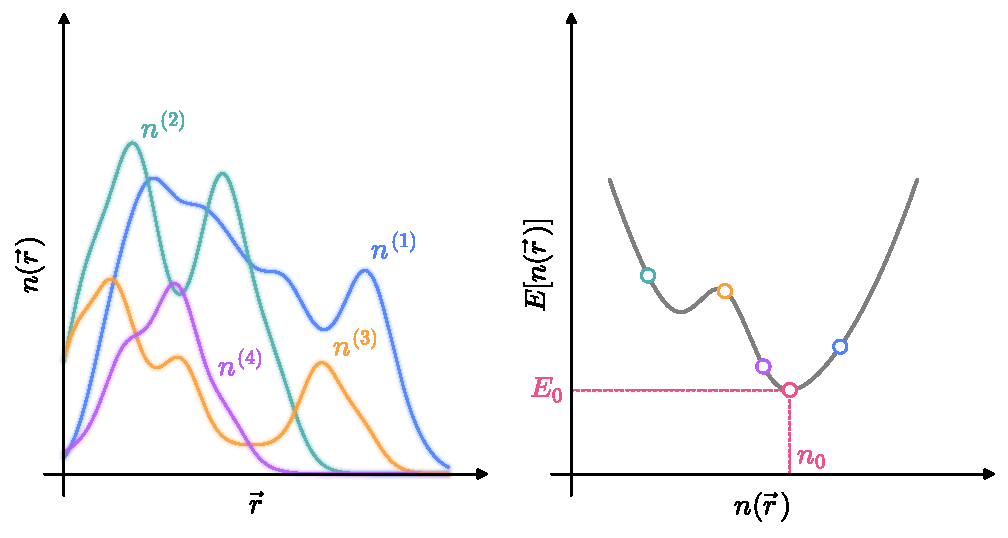
\includegraphics[width=0.85\textwidth]{figures_ch2/2.0_HK_variational_serif.pdf}
  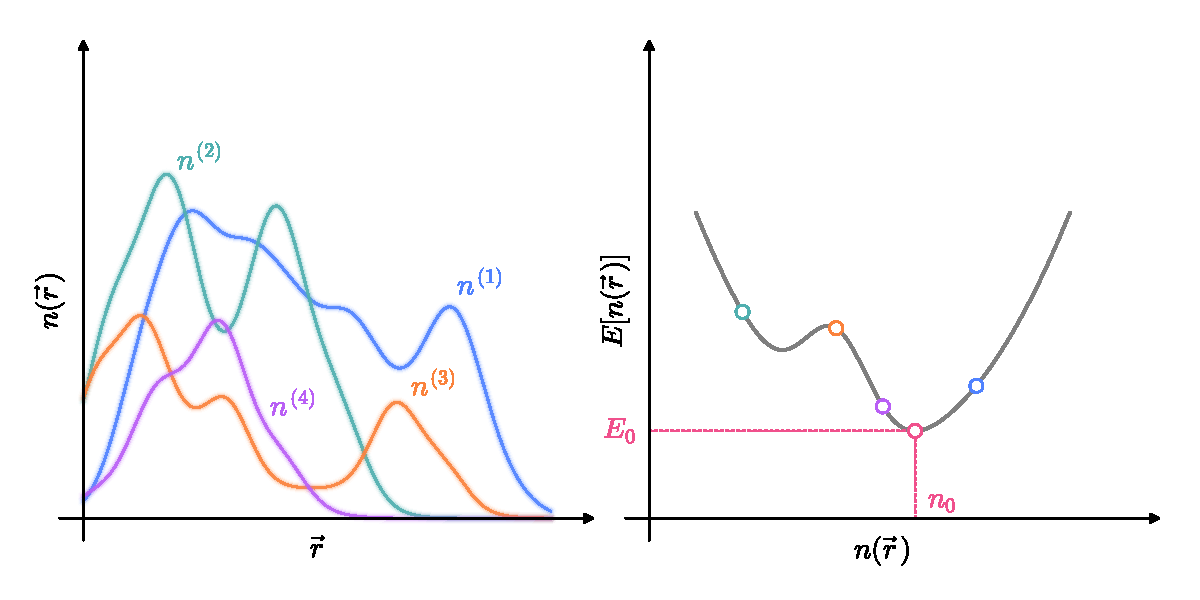
\includegraphics[width=1.0\textwidth]{figures_ch2/2.0_HK.pdf}
\caption{Schematic illustration of the Hohenberg--Kohn variational picture.}
\label{figure_HK_variational}
\end{figure}

Although density functional theory is not usually implemented in this form in practical calculations, this formulation provides a clear variational picture of the underlying idea.

We now turn to the constrained minimization in equation~\eqref{density_minimization_principle}. To enforce the fixed particle number, we impose the condition:

\begin{equation}
    \int \mathrm{d}\vec{r}\, n(\vec{r}\,) = N
\label{particle_number_constraint}
\end{equation}

by introducing a Lagrange multiplier $\mu$ and defining the auxiliary functional:

\begin{equation}
    \widetilde{E}[n]\coloneqq E[n]-\mu\left(\int\mathrm{d}\vec{r}\,n(\vec{r}\,)-N\right)
\label{lagrangian_functional_density}
\end{equation}

At the minimum, the first variation vanishes for all admissible $\delta n(\vec{r}\,)$, which gives the Euler--Lagrange condition:

\begin{equation}
    \frac{\delta E[n]}{\delta n(\vec{r}\,)} = \mu
\label{euler_lagrange_density_general}
\end{equation}

Combining the Euler--Lagrange condition in equation~\eqref{euler_lagrange_density_general} with the standard form of the energy functional in equation~\eqref{standard_form_energy_functional}, we obtain:

\begin{equation}
    \frac{\delta E_\mathrm{HK}[n]}{\delta n(\vec{r}\,)} + v_\mathrm{ext}(\vec{r}\,) = \mu
\label{euler_lagrange_density_functional}
\end{equation}

evaluated at $n=n_0$.

However, the functional $E_\mathrm{HK}[n]$ (and hence its components such as the kinetic and interaction contributions)
is not known explicitly as a functional of the density, and must be approximated in practical calculations.

At this point, we return to the standard form of the energy functional in equation~\eqref{standard_form_energy_functional}. By rearranging it, we can formally write the universal Hohenberg--Kohn functional as:

\begin{equation}
    E_\mathrm{HK}[n] = E[n]-\int\mathrm{d}\vec{r}\,v_\mathrm{ext}(\vec{r}\,)\,n(\vec{r}\,)
\label{formal_FHK_as_difference}
\end{equation}
This relation may suggest that $E_\mathrm{HK}[n]$ could be obtained once the total-energy functional $E[n]$ is known.

In practice, this is not a constructive route.
For a given $v_\mathrm{ext}(\vec{r}\,)$, the interacting many-body problem yields only the minimizing density $n_0(\vec{r}\,)$ and the corresponding energy $E[n_0]$.
To determine a functional over a broad range of densities, we would need to solve the interacting problem for many different external potentials to sample many ground-state densities.
Therefore, the Hohenberg--Kohn theorem should be viewed as an existence and uniqueness statement, rather than an explicit formula for $E_\mathrm{HK}[n]$. 

These considerations clarify why density functional theory relies on approximations.
In what follows, we introduce the Kohn--Sham construction,
which reorganizes the problem so that a large part of the functional can be treated exactly,
and the remaining unknown part can be approximated systematically.


\newpage
\section{From density functional to Kohn--Sham theory}
\label{sec:from_density_functional_to_Kohn_Sham_theory}

% opening paragraph
In practical many-body problems, an exact treatment of the hamiltonian is impossible, and approximation is inevitable.
This motivates a reformulation in terms of a simpler basic variable.

The electron density is an obvious choice.
The Thomas--Fermi kinetic energy functional in equation~\eqref{tf_functional} provides a first purely density-based model.
Its detailed construction and limitations are discussed in section~\ref{sec:appendix_thomas_fermi} of appendix~\ref{cha:appendix_quantum}.
They show that improved treatments of the kinetic energy and the exchange-correlation effects are necessary.

In what follows, we introduce an auxiliary description that retains the density as the central variable and provides a practical starting point for systematic improvements.

\subsection{Auxiliary system}

We introduce an auxiliary system that reproduces the ground-state density $n(\vec{r}\,)$ of the interacting electrons.
This maps the many-body problem onto a simpler reference description, with residual interactions captured by the exchange-correlation functional, leading to the Kohn--Sham scheme.

As shown in equation~\eqref{one-body_density}, the ground-state density can be obtained from the many-body ground-state wave function by integrating out $N-1$ coordinates.

Since one-body observables can be expressed in terms of the density, as summarized in equation~\eqref{observables_N-body}, the density provides a reduced description that avoids working directly with the full wave function. 

This approach motivates introducing an auxiliary description that reproduces the same density.

Firstly, we consider an interrelated two-body system consisting of two species.

We denote the coordinates of the first species by $x_1,x_2,\cdots,x_N$,
and those of the second species by $y_1,y_2,\cdots,y_M$.

Therefore, the full many-body wave function reads $\Psi(x_1,x_2,\cdots,x_N;y_1,y_2,\cdots,y_M)$.

Here, we suppose that there is no interaction between these two species, so that the wave function factorizes as:

\begin{equation}
    \Psi(x_1,x_2,\cdots,x_N;y_1,y_2,\cdots,y_M)
    =\psi(x_1,x_2,\cdots,x_N)\,\varphi(y_1,y_2,\cdots,y_M)
\label{separate_two-body_wave_function}
\end{equation}

In this decoupled limit, the density of the first species is obtained by integrating out the remaining coordinates.
To make the cancellation explicit, we use the normalization of $\varphi$:

\begin{equation}
    \iint\cdots\int\dif{y_1}\,\dif{y_2}\cdots\dif{y_M}\,\left|\varphi(y_1,y_2,\cdots,y_M)\right|^2 = 1
\label{phi_normalization}
\end{equation}

We define the particle density associated with $\psi$ as:

\begin{equation}
    n_\psi(x)\coloneqq N\iint\cdots\int\dif{x_2}\,\dif{x_3}\cdots\dif{x_N}\,\left|\psi(x,x_2,\cdots,x_N)\right|^2
\label{density_first_species_psi}
\end{equation}

With these definitions, we can express the density of the first species as:

\begin{equation}
    n(x)=n_\psi(x)\iint\cdots\int\dif{y_1}\,\dif{y_2}\cdots\dif{y_M}\,\left|\varphi(y_1,y_2,\cdots,y_M)\right|^2
\label{two_body_density_factorized}
\end{equation}

Applying the normalization of $\varphi$~\eqref{phi_normalization},
therefore, we arrive at:

\begin{equation}
\begin{aligned}
    n(x)
    =& \,n_\psi(x) \\
    =& \,N\iint\cdots\int\dif{x_2}\,\dif{x_3}\cdots\dif{x_N}\,\left|\psi(x,x_2,\cdots,x_N)\right|^2
\end{aligned}
\label{one_body_density_from_many_body_wave_function}
\end{equation}

In general, interactions entangle the two species and the factorization in equation~\eqref{separate_two-body_wave_function} is no longer available.
The density of one species must then be constructed from the full many-body wave function by integrating out the other degrees of freedom.
This illustrates why reduced quantities such as densities are natural objects in many-body physics.

Secondly, suppose that we work at fixed nuclear coordinates $\{\vec{R}_I\}$ and obtain the electronic hamiltonian within the Born--Oppenheimer approximation in equation~\eqref{clamped_nuclei_many_body_hamiltonian}.

In this situation, the nuclei act as fixed sources of the external potential, and the problem degenerates to an interacting electron system in the prescribed potential $v_\mathrm{ext}(\vec{r}\,)$.
The many-body wave function therefore depends only on the electronic coordinates, while the ionic positions enter as parameters.

Therefore, the auxiliary system should be viewed as a simpler description that approximates the target interacting system at the level of selected observables.
In our discussion, the density is the central observable, and the auxiliary system is required to reproduce the same density as the original problem.

Moreover, the choice of observables determines how the auxiliary system must be constructed.
If we aim to describe the density, the auxiliary system must have enough flexibility to match the density, but it is not required to reproduce the full many-body wave function.

Accordingly, once an auxiliary system is specified, its predictions should be trusted only for those quantities it is designed to reproduce.
For questions outside this design target, the auxiliary system provides no guarantee of accuracy.

Subsequently, we consider an interacting many-electron system and its corresponding auxiliary system.

The difficulty comes from the electron-electron interaction.
In the auxiliary system, we drop this interaction and compensate for it by adjusting a one-body potential.

Therefore, the problem can be stated as follows.
For a given interacting system with a density $n(\vec{r}\,)$, we seek a non-interacting system with a tuned potential that reproduces exactly the same density.
Here we ask only for the density and nothing else.
In what follows, we examine whether there is any obstacle to this construction.

Next, let us recall the Born--Oppenheimer hamiltonian in equation~\eqref{clamped_nuclei_many_body_hamiltonian}, 
and write the many-electron Schrödinger equation for the interacting system.

To make the role of $E_\mathrm{NN}(\{\vec{R}_I\})$ explicit,
we separate $\hat{H}_\mathrm{BO}(\{\vec{R}_I\})$ into an electronic operator $\hat{H}_\mathrm{el}(\{\vec{R}_I\})$ and the constant nucleus-nucleus term.
Then, we write the eigenvalue equation as:

\begin{equation}
\begin{aligned}
    \hat{H}_\mathrm{BO}(\{\vec{R}_I\})\ket{\Psi}
    &= E_\mathrm{BO}(\{\vec{R}_I\})\ket{\Psi} \\
    &= [\hat{H}_\mathrm{el}(\{\vec{R}_I\}) + E_\mathrm{NN}(\{\vec{R}_I\})]\ket{\Psi}
\end{aligned}
\label{BO_SE_with_ENN}
\end{equation}

Since $E_\mathrm{NN}(\{\vec{R}_I\})$ is a constant with respect to the electronic degrees of freedom, it only shifts the eigenvalue, and equation~\eqref{BO_SE_with_ENN} is equivalent to:

\begin{equation}
    \hat{H}_\mathrm{el}(\{\vec{R}_I\})\ket{\Psi}
    = [E_\mathrm{BO}(\{\vec{R}_I\}) - E_\mathrm{NN}(\{\vec{R}_I\})]\ket{\Psi}
\label{BO_SE_shift_ENN}
\end{equation}

In what follows, we absorb this constant shift into the eigenvalue and denote the electronic energy by:

\begin{equation}
    E\coloneqq E_\mathrm{BO}(\{\vec{R}_I\})-E_\mathrm{NN}(\{\vec{R}_I\})
\label{absorbed_electronic_energy}
\end{equation}

with this convention, the Schrödinger equation in the coordinate representation reads:

\begin{equation}
    \left(-\frac{1}{2}\sum_i\nabla_i^2
    + \sum_i v_{\mathrm{ext}}(\hat{\vec{r}}_i\,)
    + \sum_{i<j}\frac{1}{|\vec{r}_i - \vec{r}_j\,|}\right)\Psi(\vec{r}_1,\vec{r}_2,\cdots,\vec{r}_N\,)= E\,\Psi(\vec{r}_1,\vec{r}_2,\cdots,\vec{r}_N\,)
\label{BO_hamiltonian_SE}
\end{equation}

here, $E$ and $\Psi$ denote the electronic eigenvalue and eigenstate of interest at fixed nuclear coordinates $\{\vec{R}_I\}$,
where the constant term $E_\mathrm{NN}(\{\vec{R}_I\})$ has been absorbed into $E$.
In particular, the ground state determines the target density $n(\vec{r}\,)$ through equation~\eqref{one-body_density}.

Moreover, we introduce a non-interacting auxiliary system by dropping the electron-electron interaction,
and compensating for its effect through a tuned one-body potential $v_\mathrm{aux}(\vec{r}\,)$:

\begin{equation}
    \left(-\frac{1}{2}\sum_i\nabla_i^2
    + \sum_i v_\mathrm{aux}(\hat{\vec{r}}_i\,)\right)\Psi_\mathrm{aux}(\vec{r}_1,\vec{r}_2,\cdots,\vec{r}_N\,)= E_\mathrm{aux}\Psi_\mathrm{aux}(\vec{r}_1,\vec{r}_2,\cdots,\vec{r}_N\,)
\label{BO_hamiltonian_aux}
\end{equation}

here, $\Psi_\mathrm{aux}$ denotes the auxiliary many-body wave function and $E_\mathrm{aux}$ represents the corresponding eigenvalue.

The density of the auxiliary system is obtained by integrating out $N-1$ coordinates:

\begin{equation}
    n_\mathrm{aux}(\vec{r}\,)\coloneqq
    N\iint\cdots\int\dif{\vec{r}_2}\,\dif{\vec{r}_3}\cdots\dif{\vec{r}_N}\,
    \left|\Psi_\mathrm{aux}(\vec{r},\vec{r}_2,\cdots,\vec{r}_N\,)\right|^2
\label{density_aux}
\end{equation}

Hence, we define the auxiliary potential $v_\mathrm{aux}(\vec{r}\,)$ through the density-matching condition:

\begin{equation}
n_\mathrm{aux}(\vec{r}\,) = n(\vec{r}\,)
\label{auxiliary_density_matching_condition}
\end{equation}

Consequently, the question becomes whether we can construct a potential $v_\mathrm{aux}(\vec{r}\,)$ that gives the same density and, if we can, whether that potential is unique.

Finally, for a non-interacting auxiliary system, the many-body wave function can be constructed from a set of single-particle orbitals.
Accordingly, we introduce orbitals $\varphi^\mathrm{aux}_l(\vec{r}\,)$ that satisfy the one-body Schrödinger equation:

\begin{equation}
    \left[-\frac{\nabla^2}{2}+v_\mathrm{aux}(\vec{r}\,)\right]
    \varphi^\mathrm{aux}_l(\vec{r}\,)
    = \varepsilon^\mathrm{aux}_l\,\varphi^\mathrm{aux}_l(\vec{r}\,)
\label{aux_single_particle_equation}
\end{equation}

The auxiliary density is then expressed in terms of these orbitals as:

\begin{equation}
    n_\mathrm{aux}(\vec{r}\,) = \sum_l f_l\left|\varphi^\mathrm{aux}_l(\vec{r}\,)\right|^2
\label{aux_density_orbitals}
\end{equation}

here, $f_l$ denotes the occupation number of the orbital $\varphi^\mathrm{aux}_l$.

At this stage, we do not try to reproduce the full many-body wave function of the interacting system;
instead, we tune the one-body potential $v_\mathrm{aux}(\vec{r}\,)$ in the auxiliary system so that its density matches the target density:

\begin{equation}
    n_\mathrm{aux}(\vec{r}\,;v_\mathrm{aux}) = n(\vec{r}\,)
\label{auxiliary_density_matching_condition_with_potential}
\end{equation}
 
In other words, we start from a given density $n(\vec{r}\,)$ and ask whether we can find a potential $v_\mathrm{aux}(\vec{r}\,)$ that makes a non-interacting system reproduce it.

This is the basic existence question behind the auxiliary construction,
and it is often referred to as non-interacting $v$-representability~\cite{de2012pure}.

\subsection{The framework of the Kohn--Sham equations}

Firstly, we introduce a non-interacting reference system that reproduces the density $n(\vec{r}\,)$, and denote its ground-state wave function by $\Psi_\mathrm{s}[n]$.

The wave function $\Psi[n]$ denotes the minimizing interacting many-body wave function that yields the density $n(\vec{r}\,)$,
while $\Psi_\mathrm{s}[n]$ represents the ground state of a non-interacting reference system constructed to reproduce the same density.

Accordingly, they share the same one-body density but represent different many-body states:

\begin{equation}
n(\vec{r}\,) = n_{\Psi}(\vec{r}\,) = n_{\Psi_\mathrm{s}}(\vec{r}\,)
\label{density_equal_Psi_Psis}
\end{equation}

In other words, $\Psi_\mathrm{s}[n]$ is introduced to match the density, rather than to approximate $\Psi[n]$ at the wave function level.

We define the non-interacting kinetic energy functional as:

\begin{equation}
    K_\mathrm{s}[n]\coloneqq\bra{\Psi_\mathrm{s}[n]}\hat{T}\ket{\Psi_\mathrm{s}[n]}
\label{Ts_definition}
\end{equation}

Recall the Slater determinant representation~\eqref{slater_determinant}.
For the non-interacting reference state $\Psi_\mathrm{s}[n]$,
the expectation value of the kinetic energy operator becomes a sum over orbitals:

\begin{equation}
    \bra{\Psi_\mathrm{s}[n]}\hat{T}\ket{\Psi_\mathrm{s}[n]}
    = -\frac{1}{2}\sum_i f_i\,\bra{\psi_i}\nabla^2\ket{\psi_i} 
\label{Ts_orbital_sum}
\end{equation}

here, $f_i$ denotes the occupation number of the spin-orbital $\psi_i$ and satisfies:

\begin{equation}
\left\{
\begin{aligned}
    &0\le f_i\le 1              &&\qquad  \text{Pauli bound} \\
    &\textstyle{\sum_i}f_i = N  &&\qquad  \text{particle-number constraint}
\end{aligned}
\right.
\qquad
\label{occupation_constraints}
\end{equation}

Moreover, we can express the density with $f_i$:

\begin{equation}
    n(\vec{r}\,)=\sum_i f_i |\psi_i(\vec{r}\,)|^2
\label{density_with_occupation_number}
\end{equation}

here, $\psi_i(\vec{r}\,)$ denotes a spin-orbital, and the spin degree of freedom is included implicitly in the index $i$,
and the density $n(\vec{r}\,)$ can be understood as a functional of the set of spin-orbitals $\{\psi_i(\vec{r}\,)\}$.

For comparison, the kinetic energy functional $K[n]$ appearing in the Hohenberg--Kohn functional $E_\mathrm{HK}[n]$ is evaluated on the minimizing interacting many-body state $\Psi[n]$ that yields the same density.
In general, $K[n]$ and $K_\mathrm{s}[n]$ are not equal, and we write their difference as:

\begin{equation}
    K[n]=K_\mathrm{s}[n]+K_\mathrm{c}[n]
\label{T_decomposition}
\end{equation}

here, $K_\mathrm{c}[n]$ measures the kinetic correlation beyond the non-interacting reference.
We name it the kinetic-correlation functional.

At the level of the interaction energy, the Hartree approximation replaces $E_\mathrm{int}[n]$ with the classical Coulomb functional $E_\mathrm{H}[n]$ in equation~\eqref{hartree_functional}.

To obtain a fully orbital-based reference functional,
we further replace the interacting kinetic energy functional $K[n]$ by $K_\mathrm{s}[n]$,
which amounts to neglecting the kinetic correlation $K_\mathrm{c}[n]$ in equation~\eqref{T_decomposition}.

Therefore, the Hartree approximation to the total-energy functional reads:

\begin{equation}
    E_\mathrm{H}^\mathrm{tot}[n]
    = K_\mathrm{s}[n]
    + \int \dif{\vec{r}}\,v_\mathrm{ext}(\vec{r}\,)n(\vec{r}\,)
    + E_\mathrm{H}[n]
\label{hartree_total_energy_functional}
\end{equation}

Secondly, to go beyond the Hartree approximation,
we collect the missing contributions into an exchange-correlation functional.

The interaction energy functional can be written as a Hartree term plus a remainder,
$E_\mathrm{xc}^{\mathrm{int}}[n]\coloneqq E_\mathrm{int}[n]-E_\mathrm{H}[n]$,
as in equation~\eqref{Exc_int_definition} of appendix~\ref{cha:appendix_quantum}.

In the Kohn--Sham construction, there is an additional correction coming from the kinetic energy, since $K[n]$ and $K_\mathrm{s}[n]$ are not equal, and their difference is measured by $K_\mathrm{c}[n]$ in equation~\eqref{T_decomposition}.

Therefore, we define the Kohn--Sham exchange-correlation functional as:

\begin{equation}
    E_\mathrm{xc}[n]\coloneqq K_\mathrm{c}[n]+E_\mathrm{xc}^{\mathrm{int}}[n]
\label{Exc_KS_sum}
\end{equation}

According to the definition of universal Hohenberg--Kohn functional~\eqref{functional_HK_definition}, 
and the exchange-correlation part of the interaction energy functional~\eqref{Exc_int_definition},
we have:

\begin{equation}
\begin{aligned}
    E_\mathrm{xc}[n]
    &= (K[n]-K_\mathrm{s}[n]) + (E_\mathrm{int}[n]-E_\mathrm{H}[n]) \\
    &= (K[n]-K_\mathrm{s}[n]) + (E_\mathrm{HK}[n]-K[n]-E_\mathrm{H}[n]) \\
    &= E_\mathrm{HK}[n]-K_\mathrm{s}[n]-E_\mathrm{H}[n]
\end{aligned}
\label{Exc_KS_definition}
\end{equation}

Let us perform some manipulations on the exact ground-state energy functional~\eqref{energy_density_functional_decomposition}:

\begin{equation}
\begin{aligned}
    E[n] &= K[n]+E_\mathrm{int}[n]
    +\int\mathrm{d}\vec{r}\,v_\mathrm{ext}(\vec{r}\,)\,n(\vec{r}\,) \\
    &= E_\mathrm{HK}[n]
    + \int\mathrm{d}\vec{r}\,v_\mathrm{ext}(\vec{r}\,)\,n(\vec{r}\,)
    + K_\mathrm{s}[n] - K_\mathrm{s}[n] + E_\mathrm{H}[n] - E_\mathrm{H}[n] \\
    &= K_\mathrm{s}[n] +
    \int\mathrm{d}\vec{r}\,v_\mathrm{ext}(\vec{r}\,)\,n(\vec{r}\,)
    + E_\mathrm{H}[n] + (E_\mathrm{HK}[n]-K_\mathrm{s}[n]-E_\mathrm{H}[n])
\end{aligned}
\label{energy_density_functional_manipulations}
\end{equation}

Recalling the Kohn--Sham exchange-correlation functional~\eqref{Exc_KS_definition}
and the Hartree approximation to the total-energy functional~\eqref{hartree_total_energy_functional},
we obtain:

\begin{equation}
\begin{aligned}
    E[n] &= K_\mathrm{s}[n]
    + \int\mathrm{d}\vec{r}\,v_\mathrm{ext}(\vec{r}\,)\,n(\vec{r}\,)
    + E_\mathrm{H}[n] + E_\mathrm{xc}[n] \\
    &= K_\mathrm{s}[n]
    + \int\mathrm{d}\vec{r}\,v_\mathrm{ext}(\vec{r}\,)\,n(\vec{r}\,)
    + \frac{1}{2}\iint\dif{\vec{r}}\,\dif{\vec{r}\,'}\,\frac{n(\vec{r}\,)n(\vec{r}\,')}{|\vec{r}-\vec{r}\,'|}
    + E_\mathrm{xc}[n] \\
    &= E_\mathrm{H}^\mathrm{tot}[n] + E_\mathrm{xc}[n]
\end{aligned}
\end{equation}

Subsequently, we minimize the energy functional $E[n]$ with respect to the spin-orbital wave functions $\psi_i(\vec{r}\,)$.
This variational procedure determines the stationary condition of the functional, while enforcing the orthonormality constraints.

Accordingly, we introduce a set of Lagrange multipliers $\{\lambda_{ij}\}$ and consider the constrained variation.
Varying with respect to $\psi_i^\ast(\vec{r}\,)$ generates a one-body eigenvalue problem.
The detailed derivation is given in subsection~\ref{subsec:KS_variational_derivation}.

Moreover, the functional derivative of the Hartree term produces the Hartree potential:

\begin{equation}
    v_\mathrm{H}([n];\vec{r}\,)
    \coloneqq \frac{\delta E_\mathrm{H}[n]}{\delta n(\vec{r}\,)}
    = \int\dif{\vec{r}\,'}\,\frac{n(\vec{r}\,')}{|\vec{r}-\vec{r}\,'|}
\label{Hartree_potential_KS_definition}
\end{equation}

Similarly, the exchange-correlation contribution defines the exchange-correlation potential as its functional derivative:

\begin{equation}
    v_\mathrm{xc}([n];\vec{r}\,)\coloneqq\frac{\delta E_\mathrm{xc}[n]}{\delta n(\vec{r}\,)}
\label{xc_potential_definition}
\end{equation}

It is therefore convenient to introduce the effective Kohn--Sham potential:

\begin{equation}
    v_\mathrm{eff}([n];\vec{r}\,)
    \coloneqq v_\mathrm{ext}(\vec{r}\,)
    + v_\mathrm{H}([n];\vec{r}\,)
    + v_\mathrm{xc}([n];\vec{r}\,)
\label{KS_effective_potential_definition}
\end{equation}

here, the corresponding one-body operator is $\hat{v}_\mathrm{eff}\coloneqq v_\mathrm{eff}([n];\hat{\vec{r}}\,)$.

Next, in a basis where the Lagrange-multiplier matrix is diagonal,
the stationarity condition can be expressed as the Kohn--Sham equations~\cite{kohn1965self}:

\begin{equation}
    \left[-\frac{1}{2}\nabla^2+v_\mathrm{eff}([n];\vec{r}\,)\right]\psi_i(\vec{r}\,)
    = \lambda_i\,\psi_i(\vec{r}\,)
\label{KS_equation}
\end{equation}

here, the orbitals are determined by the effective potential $v_\mathrm{eff}([n];\vec{r}\,)$.
Therefore, at self-consistency, we may write:

\begin{equation}
    \psi_i(\vec{r}\,)=\psi_i([n];\vec{r}\,)
\label{KS_orbitals_as_density_functionals}
\end{equation}

The Kohn--Sham density expression~\eqref{density_with_occupation_number} gives $n(\vec{r}\,)$ once the orbitals are known.
Meanwhile, $v_\mathrm{eff}([n];\vec{r}\,)$ depends on $n(\vec{r}\,)$ through equation~\eqref{KS_effective_potential_definition}.
Therefore, we solve equations~\eqref{KS_effective_potential_definition} and~\eqref{KS_equation} self-consistently.

In this sense, density functional theory is built on the Hohenberg--Kohn theorem.
It states that the ground-state density uniquely determines the external potential modulo an additive constant~\cite{hohenberg1964inhomogeneous,kohn1999nobel}.
Meanwhile, the density and the external potential are in bijective correspondence:

\begin{equation}
    n(\vec{r}\,)
    \,\longleftrightarrow\,
    \left[v_\mathrm{ext}(\vec{r}\,)\right]
\label{HK_density_potential_correspondence}
\end{equation}

In the Kohn--Sham auxiliary system, the electrons are non-interacting.
Therefore, the only potential entering the one-body hamiltonian is the effective potential $v_\mathrm{eff}([n];\vec{r}\,)$.
It plays the role of the external potential for the auxiliary system.

Consequently, we may also view the Kohn--Sham potential as being uniquely linked to the density:

\begin{equation}
    n(\vec{r}\,)
    \,\longleftrightarrow\,
    \left[v_\mathrm{eff}([n];\vec{r}\,)\right]
\label{KS_density_potential_correspondence}
\end{equation}

here, $\left[v(\vec{r}\,)\right]$ denotes the equivalence class of potentials that differ only by an additive constant.

This shows that once the density $n(\vec{r}\,)$ is given, the effective potential $v_\mathrm{eff}([n];\vec{r}\,)$ is fixed up to an additive constant.

Therefore, in this non-interacting Kohn--Sham auxiliary system, we regard the corresponding total ground-state energy as a functional of the density, and denote it by $E_\mathrm{s}[n]$.

For the auxiliary non-interacting system, we achieve the Kohn--Sham auxiliary energy functional:

\begin{equation}
    E_\mathrm{s}[n]=K_\mathrm{s}[n]+\int\dif{\vec{r}}\,n(\vec{r}\,)v_\mathrm{eff}([n];\vec{r}\,)
\label{KS_auxiliary_energy_functional}
\end{equation}

Moreover, we recall the exact energy decomposition in equation~\eqref{energy_density_functional_decomposition},
together with the Hohenberg--Kohn correspondence in equation~\eqref{hk_correspondence_v_n_psi}.
They tell us that the ground-state energy can be viewed as a functional of the density.

Hence, we introduce the key idea of the Kohn--Sham equations.
For a given interacting system, we assume the existence of an auxiliary system of non-interacting electrons.
This auxiliary system is constructed to reproduce the same density:

\begin{equation}
    n_\mathrm{s}(\vec{r}\,)=n(\vec{r}\,)
\label{KS_same_density_assumption}
\end{equation}

here, $n_\mathrm{s}(\vec{r}\,)$ denotes the ground-state density of the auxiliary non-interacting system,
which is obtained from a set of one-electron orbitals.
The corresponding one-body potential is denoted by the Kohn--Sham potential $v_\mathrm{eff}([n];\vec{r}\,)$.
It is chosen such that equation~\eqref{KS_same_density_assumption} holds.

Consequently, the interacting many-electron problem is mapped to a non-interacting orbital problem with the same density.

\subsection{From variational derivation to the Kohn--Sham equations}
\label{subsec:KS_variational_derivation}

To determine the orbitals in the Kohn--Sham scheme,
we start from the density built from orbitals in equation~\eqref{density_with_occupation_number}.
We are going to apply the variational principle and minimize the total energy with respect to the orbitals.

Firstly, we introduce the one-body kinetic operator in the single-particle Hilbert space:

\begin{equation}
    \hat{K}\coloneqq
    -\frac{1}{2}\nabla^2
\label{KS_one_body_kinetic_operator_definition}
\end{equation}

Accordingly, we represent the non-interacting kinetic energy as an orbital functional:

\begin{equation}
    K_\mathrm{s}[\{\psi_i(\vec{r}\,)\}]=
    \sum_i f_i \bra{\psi_i}\hat{K}\ket{\psi_i}
\label{KS_noninteracting_kinetic_energy_orbital_functional}
\end{equation}

Next, we define the one-body external potential operator:

\begin{equation}
    \hat{v}_\mathrm{ext}\coloneqq
    v_\mathrm{ext}(\hat{\vec{r}}\,)
\label{KS_one_body_external_operator_definition}
\end{equation}

In coordinate representation, the corresponding orbital expectation value reads:

\begin{equation}
    \bra{\psi_i}\hat{v}_\mathrm{ext}\ket{\psi_i}=
    \int\dif{\vec{r}}\,
    \psi_i^\ast(\vec{r}\,)v_\mathrm{ext}(\vec{r}\,)\psi_i(\vec{r}\,)
\label{KS_external_operator_expectation_coordinate}
\end{equation}

Afterwards, using the Kohn--Sham density expression in equation~\eqref{density_with_occupation_number},
we express the external potential energy in the orbital form:

\begin{equation}
    \int\dif{\vec{r}}\,n(\vec{r}\,)v_\mathrm{ext}(\vec{r}\,)
    = \sum_{i}f_{i}\bra{\psi_i}\hat{v}_\mathrm{ext}\ket{\psi_i}
\label{KS_external_energy_orbital_form}
\end{equation}

Therefore, we view the total energy as an orbital functional through the density $n(\vec{r}\,)$:

\begin{equation}
    E[\{\psi_i(\vec{r}\,)\}]\coloneqq
    \,K_\mathrm{s}[\{\psi_i(\vec{r}\,)\}]
    + \int \dif{\vec{r}}\,
    n(\vec{r}\,)v_\mathrm{ext}(\vec{r}\,) 
    \,+ E_\mathrm{H}[n]
    + E_\mathrm{xc}[n]
\label{KS_total_energy_orbital_functional}
\end{equation}

here, we reiterate that the density $n(\vec{r}\,)$ is understood as a functional of the set of spin-orbitals $\{\psi_i(\vec{r}\,)\}$ through equation~\eqref{density_with_occupation_number}.

Secondly, we impose the orthonormality constraints:

\begin{equation}
    \braket{\psi_i|\psi_j}=\delta_{ij}
\label{KS_orbital_orthonormality}
\end{equation}

Accordingly, we introduce a matrix of Lagrange multipliers $\lambda_{ij}$ and define this constrained functional:

\begin{equation}
    \mathcal{F}[\{\psi_i(\vec{r}\,)\}]\coloneqq
    E[\{\psi_i(\vec{r}\,)\}]
    -\sum_{i,j}\lambda_{ij}\left(\braket{\psi_i|\psi_j}-\delta_{ij}\right)
\label{KS_constrained_functional_orbitals}
\end{equation}

Thirdly, we require stationarity with respect to the orbitals:

\begin{equation}
    \frac{\delta\mathcal{F}[\{\psi_i(\vec{r}\,)\}]}{\delta\bra{\psi_i}}=0
\label{KS_stationarity_condition_orbitals}
\end{equation}

here, we vary with respect to $\bra{\psi_i}$, treating $\ket{\psi_i}$ and $\bra{\psi_i}$ as independent variables.

Moreover, we use the density dependence on the orbitals.
In coordinate representation, equation~\eqref{density_with_occupation_number} shows:

\begin{equation}
    \frac{\delta n(\vec{r}\,)}{\delta \psi_i^\ast(\vec{r}\,)}
    =f_i\,\psi_i(\vec{r}\,)
\label{KS_density_orbital_derivative}
\end{equation}

Next, we collect the potential terms including
the Hartree potential $v_\mathrm{H}([n];\vec{r}\,)$ in equation~\eqref{Hartree_potential_KS_definition},
and the exchange-correlation potential $v_\mathrm{xc}([n];\vec{r}\,)$ in equation~\eqref{xc_potential_definition}.
Together with the external potential, they form the Kohn--Sham effective potential $v_\mathrm{eff}([n];\vec{r}\,)$ in equation~\eqref{KS_effective_potential_definition}.

Accordingly, we combine the kinetic term and the effective potential into a single one-body operator.
This allows us to write the Kohn--Sham equations in a compact form.
Therefore, we define the Kohn--Sham one-body operator as:

\begin{equation}
    \hat{h}_\mathrm{KS}\coloneqq
    \hat{K}+\hat{v}_\mathrm{eff}
\label{KS_one_body_hamiltonian_definition}
\end{equation}

Finally, from the stationarity condition in equation~\eqref{KS_stationarity_condition_orbitals},
we obtain a set of one-particle equations:

\begin{equation}
    \hat{h}_\mathrm{KS}\ket{\psi_i} =
    \sum_j\lambda_{ij}\ket{\psi_j}
\label{KS_equation_general_dirac}
\end{equation}

Accordingly, we take $\lambda_{ij}$ to be Hermitian and diagonalize it in a chosen basis.
Equation~\eqref{KS_equation_general_dirac} then reduces to the standard eigenvalue form:

\begin{equation}
    \hat{h}_\mathrm{KS}\ket{\psi_i} =
    \lambda_i\ket{\psi_i}
\label{KS_equation_diagonal_dirac}
\end{equation}

In coordinate representation, using equation~\eqref{KS_equation_diagonal_dirac}, we get the Kohn--Sham equations~\eqref{KS_equation}.
For ease of understanding and calculation, we expand the Kohn--Sham equation~\eqref{KS_equation} as:

\begin{equation}
\begin{aligned}
    \lambda_i\,\psi_i(\vec{r}\,)
    &=\left[
    -\frac{1}{2}\nabla^2
    +v_\mathrm{ext}(\vec{r}\,)
    +v_\mathrm{H}([n];\vec{r}\,)
    +v_\mathrm{xc}([n];\vec{r}\,)
    \right]\psi_i(\vec{r}\,) \\
    &=\left[
    -\frac{1}{2}\nabla^2
    +v_\mathrm{ext}(\vec{r}\,)
    +\int\dif{\vec{r}\,'}\,\frac{n(\vec{r}\,')}{|\vec{r}-\vec{r}\,'|}
    +\frac{\delta E_\mathrm{xc}[n]}{\delta n(\vec{r}\,)}
    \right]\psi_i(\vec{r}\,)
\end{aligned}
\label{KS_equations_expansion}
\end{equation}

Consequently, we have obtained the one-particle equations for the auxiliary non-interacting system,
which means each electron moves in the effective potential $v_\mathrm{eff}([n];\vec{r}\,)$.

Together with equation~\eqref{density_with_occupation_number},
we can solve the Kohn--Sham equations~\eqref{KS_equations_expansion},
and achieve the exact ground-state density of the interacting system.

\subsection{Variational construction of the Kohn--Sham scheme}

The previous subsection derived the Kohn--Sham equations by varying the orbitals directly. Here we complement that derivation by showing, at the density-functional level, why the auxiliary non-interacting construction is variationally consistent.

We start from the interacting ground-state density $n_0(\vec{r}\,)$, which makes the exact energy functional stationary.

However, we introduce an auxiliary non-interacting energy functional and require that it is minimized by $n_0(\vec{r}\,)$.
This gives an auxiliary independent-particle system with the same ground-state density.
Then an effective potential exists, and the Kohn--Sham equations follow.

Let us start from the Kohn--Sham auxiliary energy functional in equation~\eqref{KS_auxiliary_energy_functional}.
We search its minimum among admissible densities,
and impose the corresponding positivity and normalization conditions:

\begin{equation}
\left\{
\begin{aligned}
    &n(\vec{r}\,) \ge 0 \\
    &\int\dif{\vec{r}}\,n(\vec{r}\,) = N
\end{aligned}\right.
\label{admissible_density_conditions}
\end{equation}

Accordingly, we impose the normalization constraint by a Lagrange multiplier $\lambda$ and require stationarity:

\begin{equation}
    \frac{\delta}{\delta n(\vec{r}\,)}\,\left[
        E_\mathrm{s}[n]-\lambda\int\dif{\vec{r}\,'}\,n(\vec{r}\,')
    \right]=0
\label{KS_auxiliary_density_stationarity}
\end{equation}

Therefore, at the minimizing density $n_0(\vec{r}\,)$,
we obtain the Euler--Lagrange condition for the auxiliary non-interacting energy functional $E_\mathrm{s}[n]$:

\begin{equation}
    \left.\frac{\delta K_\mathrm{s}[n]}{\delta n(\vec{r}\,)}\right|_{n_0}+v_\mathrm{eff}([n_0];\vec{r}\,)=\lambda
\label{KS_auxiliary_EL_condition}
\end{equation}

here, $\lambda$ is treated as a constant.

Therefore, we equivalently express the Euler--Lagrange condition as an explicit expression for the effective potential $v_\mathrm{eff}([n_0];\vec{r}\,)$:

\begin{equation}
    v_\mathrm{eff}([n_0];\vec{r}\,)
    = \lambda-\left.\frac{\delta K_\mathrm{s}[n]}{\delta n(\vec{r}\,)}\right|_{n_0}
    = -\left.\frac{\delta K_\mathrm{s}[n]}{\delta n(\vec{r}\,)}\right|_{n_0}+\mathrm{const.}
\label{KS_auxiliary_v_eff_from_Ts}
\end{equation}

Consequently, if the functional derivative of the non-interacting kinetic energy functional $K_\mathrm{s}[n]$ is well behaved around the ground-state density $n_0(\vec{r}\,)$,
the Kohn--Sham effective potential $v_\mathrm{eff}(\vec{r}\,)$ can be constructed to reproduce $n_0(\vec{r}\,)$.
In this sense, the auxiliary non-interacting system idea is reasonable.

In principle, the Kohn--Sham equations give the exact electron density~\cite{wagner2014kohn}.
The only missing piece is the exchange-correlation energy functional $E_\mathrm{xc}[n]$, or equivalently the exchange-correlation potential $v_\mathrm{xc}([n];\vec{r}\,)$.
We will introduce approximations for it later.

\subsection{Remarks on the Kohn--Sham solutions}

In practical applications, we have to solve the Kohn--Sham equations~\eqref{KS_equations_expansion}.
Once the Kohn--Sham one-body operator is specified,
we diagonalize it and obtain the eigenvalues $\lambda_i$ and eigenvectors $\ket{\psi_i}$.
We then construct the electron density through equation~\eqref{density_with_occupation_number}.

However, the density $n(\vec{r}\,)$ is both an output and an input.
To build the Kohn--Sham operator, we need the Hartree potential $v_\mathrm{H}([n];\vec{r}\,)$,
and the exchange-correlation potential $v_\mathrm{xc}([n];\vec{r}\,)$.
Both of them depend on the density.
Therefore, the Kohn--Sham equations are solved self-consistently.

Consequently, we utilize an iterative self-consistent field scheme.
Let us start from a trial density.
We construct the potentials and diagonalize the Kohn--Sham operator.
This generates updated orbitals and a new density.
We repeat these steps until the density is converged.
This idea goes back to Hartree and his self-consistent treatment~\cite{hartree1928wave}.

Next, we comment on the Kohn--Sham eigenvalues $\lambda_i$.
They have the dimension of energy,
but belong to the auxiliary non-interacting system.
Therefore, in general, they are not electron removal or addition energies,
which are defined by total-energy differences.

There is an important exception for finite systems.
For the exact functional, the highest occupied Kohn--Sham eigenvalue equals the negative ionization energy~\cite{perdew1997comment, harbola1999relationship}.
For extended systems, similar interpretations have been discussed~\cite{mundt2006photoelectron},
but no general proof is available in the same simple form.

In fact, we work with approximate functionals.
The resulting eigenvalues are widely used in materials science, for instance as a useful reference for band-structure analysis.
We will return to this point later.

Afterwards, we look into the Kohn--Sham potential.
It coincides with the effective potential in equation~\eqref{KS_effective_potential_definition}.
It consists of the external potential, the Hartree potential, and the exchange-correlation potential:

\begin{equation}
    v_\mathrm{KS}([n];\vec{r}\,)
    = v_\mathrm{ext}(\vec{r}\,)
    + v_\mathrm{H}([n];\vec{r}\,)
    + v_\mathrm{xc}([n];\vec{r}\,)
\label{KS_potential_decomposition}
\end{equation}

here, the external potential $v_\mathrm{ext}(\vec{r}\,)$ is fixed by the ionic structure.
The Hartree potential $v_\mathrm{H}([n];\vec{r}\,)$ is a known functional of the density.
The main difficulty lies in the exchange-correlation potential $v_\mathrm{xc}([n];\vec{r}\,)$.

In the local Kohn--Sham formulation considered here, the exchange-correlation potential $v_\mathrm{xc}([n];\vec{r}\,)$ is a static and local potential.
In coordinate representation, it acts as a multiplicative operator.
Nevertheless, its functional dependence on the density can be highly non-trivial.
Therefore, practical density functional theory relies on approximations for the exchange-correlation energy functional $E_\mathrm{xc}[n]$,
or equivalently for $v_\mathrm{xc}([n];\vec{r}\,)$.
We will discuss these approximations later.

\subsection{Structure and construction of the Kohn--Sham potential}

After the general framework of the Kohn--Sham construction has been established through equations~\eqref{density_with_occupation_number},~\eqref{KS_equations_expansion}, and~\eqref{KS_potential_decomposition},
we examine several simple exactly solvable model systems.
These examples demonstrate the exact form that the Kohn--Sham potential can take.
They also elucidate why its exchange-correlation component can remain highly non-trivial even though it is still a local multiplicative potential.

Firstly, let us consider a one-dimensional harmonic well containing two interacting electrons.
In atomic units, the interacting problem is defined by the Schrödinger equation:

\begin{equation}
    \hat{H}\Psi(x_1,x_2)=E\Psi(x_1,x_2)
\label{interacting_Schrodinger_equation_1D_two_electrons}
\end{equation}

with the many-body hamiltonian:

\begin{equation}
    \hat{H}
    = \sum_{i=1}^{2}\left[-\frac{1}{2}\frac{\dif^2}{\dif x_i^2}+v_\mathrm{ext}(x_i)\right]
    + v_\mathrm{ee}(x_1,x_2)
\label{interacting_hamiltonian_1D_two_electrons}
\end{equation}

here, $v_\mathrm{ee}(x_1,x_2)$ denotes the two-body interaction.
In one dimension, we use the soft-Coulomb form $v_\mathrm{ee}(x_1,x_2)=\left[(x_1-x_2)^2+a^2\right]^{-1/2}$ with the softening parameter $a$.
For a harmonic confinement, the external potential takes the form:

\begin{equation}
    v_\mathrm{ext}(x)=\frac{1}{2}\Omega^2 x^2
\label{harmonic_external_potential_1D}
\end{equation}

here, $\Omega$ refers to the angular frequency of harmonic confinement.

By solving the Schrödinger equation~\eqref{interacting_Schrodinger_equation_1D_two_electrons},
we get the exact density:

\begin{equation}
    n(x)=2\int\dif{x_2}\,|\Psi(x,x_2)|^2
\label{exact_density_from_interacting_wave_function_1D}
\end{equation}

Secondly, we inquire which local Kohn--Sham potential reproduces the exact density given in equation~\eqref{exact_density_from_interacting_wave_function_1D}.

In one dimension, equations~\eqref{KS_equations_expansion} and~\eqref{density_with_occupation_number} may be written schematically as:

\begin{equation}
    \left[-\frac{1}{2}\frac{\dif^2}{\dif x^2} + v_\mathrm{KS}([n];x)\right]\psi_i(x) = \lambda_i\psi_i(x)
\label{KS_equation_1D_schematic}
\end{equation}

We denote the corresponding density function as:

\begin{equation}
    n_\mathrm{KS}(x)=\sum_i f_i |\psi_i(x)|^2
\label{KS_density_1D_schematic}
\end{equation}

The Kohn--Sham auxiliary system is designed to reproduce exactly the same ground-state electron density as the true interacting system:

\begin{equation}
    n_\mathrm{KS}(x)=n(x)
\label{KS_exact_density_matching_1D}
\end{equation}

We first test the naive choice:

\begin{equation}
    v_\mathrm{KS}([n];x)=v_\mathrm{ext}(x)
\label{naive_KS_choice_external_only_1D}
\end{equation}

With this choice, the density from equation~\eqref{KS_density_1D_schematic} is concentrated near the centre of the well.
This concentration is generally excessive.
Therefore, the missing interaction effects are encoded directly in the local Kohn--Sham potential.
In the exact solution, this potential develops a central bump~\cite{helbig2009exact}.
To isolate the interaction-induced contribution,
we define the Hartree-exchange-correlation potential:

\begin{equation}
    v_\mathrm{Hxc}([n];x)\coloneqq
    v_\mathrm{KS}([n];x)-v_\mathrm{ext}(x)
\label{Hxc_potential_definition_1D}
\end{equation}

Accordingly, we regard this central bump as a feature of the Hartree-exchange-correlation potential $v_\mathrm{Hxc}([n];x)$.
It works to suppress charge accumulation near the origin and thereby enforce equation~\eqref{KS_exact_density_matching_1D}.
Therefore, the exact Kohn--Sham potential $v_\mathrm{KS}([n];x)$ is not merely a shifted harmonic well.

Next, an asymmetric double-well potential provides an even more instructive example.
In this interacting system,
the electron-electron repulsion may force the two electrons to occupy different wells.
By contrast, in our auxiliary non-interacting system,
both electrons would tend to occupy the energetically more favourable well.

Therefore, the exact Kohn--Sham potential $v_\mathrm{KS}([n];x)$ must develop an additional structure that redistributes the charge correctly.
Schematically, this structure reads:

\begin{equation}
v_\mathrm{KS}([n];x)\approx\left\{
\begin{aligned}
    &v_\mathrm{L}(x)      &&\qquad \text{$x$ in the left well} \\
    &v_\mathrm{R}(x)+C    &&\qquad \text{$x$ in the right well}
\end{aligned}\right.
\qquad
\label{KS_step_structure_schematic}
\end{equation}

here, the approximately constant shift $C$ denotes the offset between the two spatial regions.
This step raises one well relative to the other and thereby enforces the correct density distribution~\cite{makmal2011dissociation}.

Subsequently, from the Kohn--Sham potential decomposition in equation~\eqref{KS_potential_decomposition},
the external potential has already been fixed, and the Hartree potential $v_\mathrm{H}([n];x)$ has already been defined in equation~\eqref{Hartree_potential_KS_definition}.
Therefore, the remaining freedom lies mainly in the exchange-correlation potential $v_\mathrm{xc}([n];x)$ defined in equation~\eqref{xc_potential_definition}.
Hence, the exact exchange-correlation potential $v_\mathrm{xc}([n];x)$ may contain bumps, barriers, and steps~\cite{hodgson2016origin}.
In particular, a pronounced step may appear in a low-density region.
This makes it difficult to construct accurate approximations to the exchange-correlation potential $v_\mathrm{xc}([n];x)$.

Consequently, we turn to the inverse point of view.
If an accurate density is available from an exact method, we seek a local potential that reproduces it.
This defines the inverse Kohn--Sham problem~\cite{wang1993construction, astala2006kohn}.

Let us denote the target density by $n_\mathrm{tar}(x)$.
We require:

\begin{equation}
    n_\mathrm{KS}(x)=n_\mathrm{tar}(x)
\label{inverse_KS_target_density_condition}
\end{equation}

and we take the zeroth-step Kohn--Sham potential as:

\begin{equation}
    v_\mathrm{KS}^{(0)}(x)=v_\mathrm{ext}(x)
\label{inverse_KS_initial_guess}
\end{equation}

We then solve the Kohn--Sham equation, equation~\eqref{KS_equation_1D_schematic}, and obtain the density at the $k$th iteration:

\begin{equation}
    n^{(k)}(x)=\sum_i f_i \lvert\psi_i^{(k)}(x)\rvert^2
\label{inverse_KS_density_from_kth_iteration}
\end{equation}

here, $f_i$ denotes the occupation number of the $i$th Kohn--Sham orbital $\psi_i^{(k)}(x)$.
We update the Kohn--Sham potential according to the density mismatch.
A simple schematic iteration is:

\begin{equation}
    v_\mathrm{KS}^{(k+1)}(x) = v_\mathrm{KS}^{(k)}(x)
    + \mu \left[\left(n^{(k)}(x)\right)^p - \left(n_\mathrm{tar}(x)\right)^p\right]
\label{inverse_KS_density_update}
\end{equation}

here, $\mu$ denotes a mixing parameter and $p$ denotes an additional stability parameter.

Accordingly, the Kohn--Sham potential is increased where the density is overestimated and decreased where it is underestimated.
At convergence, we arrive at:

\begin{equation}
\left\{
\begin{aligned}
    n^{(k)}(x)                &\rightarrow n_\mathrm{tar}(x)   \\
    v_\mathrm{KS}^{(k)}(x)    &\rightarrow v_\mathrm{KS}([n_\mathrm{tar}];x)
\end{aligned}\right.
\qquad
\text{as $k\rightarrow\infty$} 
\label{inverse_KS_fixed_point_condition}
\end{equation}

\subsection{The Hartree equations}

Before turning to practical approximations to $E_\mathrm{xc}$, it is useful to consider the simpler self-consistent scheme that remains when exchange and correlation are omitted. If we retain the external potential $v_\mathrm{ext}(\vec{r}\,)$ and the classical electrostatic interaction generated by the density $n(\vec{r}\,)$, then we arrive at the Hartree equations:

\begin{equation}
    \left[-\frac{1}{2}\nabla^2
        + v_\mathrm{ext}(\vec{r}\,)
        + v_\mathrm{H}([n];\vec{r}\,)\right]
    \psi_i(\vec{r}\,)
    = \lambda_i \psi_i(\vec{r}\,)
\label{Hartree_equations_expansion}
\end{equation}

here, $\lambda_i$ denotes the Hartree eigenvalue associated with the one-particle orbital $\psi_i(\vec{r}\,)$.
The Hartree potential $v_\mathrm{H}([n];\vec{r}\,)$, introduced in equation~\eqref{Hartree_potential_KS_definition}, is the classical electrostatic potential generated by the electron density $n(\vec{r}\,)$.
Since the density is still constructed from the occupied one-particle orbitals through equation~\eqref{density_with_occupation_number},
the Hartree equations~\eqref{Hartree_equations_expansion} must be solved self-consistently.

Next, the Hartree equations already demonstrate the basic one-particle structure of a self-consistent field theory.
We start from a trial density,
construct the Hartree potential $v_\mathrm{H}([n];\vec{r}\,)$,
solve equation~\eqref{Hartree_equations_expansion},
update the density through equation~\eqref{density_with_occupation_number},
and repeat these steps until convergence is reached.
In this sense, the Hartree equations already anticipate the later structure of the Kohn--Sham equations~\eqref{KS_equations_expansion}.

However, the Hartree equations remain incomplete.
The Hartree potential $v_\mathrm{H}([n];\vec{r}\,)$ contains only the classical electrostatic contribution.
It does not incorporate exchange effects or correlation effects.
Moreover, since $v_\mathrm{H}([n];\vec{r}\,)$ is generated by the total density $n(\vec{r}\,)$,
it also contains an unphysical self-interaction contribution~\cite{perdew1981self}.
Therefore, the Hartree equations do not provide an accurate description of interacting electrons.

Consequently, one must go beyond the Hartree approximation.
In the Kohn--Sham framework, this missing physics is collected into the exchange-correlation potential $v_\mathrm{xc}([n];\vec{r}\,)$ appearing in equation~\eqref{KS_potential_decomposition}.
Equivalently, it is described by the exchange-correlation energy functional $E_\mathrm{xc}[n]$.
As we have already emphasized in the previous subsection,
the main difficulty does not lie in the external potential $v_\mathrm{ext}(\vec{r}\,)$ or the Hartree potential $v_\mathrm{H}([n];\vec{r}\,)$,
but in the construction of the exchange-correlation functional itself.
Therefore, the next step is to introduce practical approximations for $E_\mathrm{xc}[n]$ and $v_\mathrm{xc}([n];\vec{r}\,)$.

\newpage
\section{Exchange-correlation functional}
\label{sec:exchange_correlation_functional}

% opening paragraph
As we have already discussed in equation~\eqref{xc_potential_definition},
the exchange-correlation potential $v_\mathrm{xc}([n];\vec{r}\,)$ is obtained from the exchange-correlation energy functional $E_\mathrm{xc}[n]$.
Moreover, from equation~\eqref{KS_potential_decomposition},
we have already seen that the external potential $v_\mathrm{ext}(\vec{r}\,)$ is fixed by the ionic structure,
and the Hartree potential $v_\mathrm{H}([n];\vec{r}\,)$ is a known functional of the density.
Therefore, in practical density functional theory,
the main difficulty lies in the construction of the exchange-correlation functional itself.

% Thereafter, we introduce several widely used approximations for the exchange-\hspace{0pt}correlation energy functional $E_\mathrm{xc}[n]$~\cite{martin2020electronic}.
Thereafter, for the exchange-correlation energy functional $E_\mathrm{xc}[n]$~\cite{martin2020electronic}, we introduce several widely used approximations.
They differ in how much information about the density is retained.
The simplest approximation depends only on the local value of the density.
Semilocal approximations also include the density gradient.
Beyond them, hybrid functionals incorporate a fraction of exact exchange.

\subsection{Local density and generalized gradient approximations}

Firstly, we consider the local density approximation.
Its basic idea is to approximate the exchange-correlation energy locally by that of a homogeneous electron gas with the same density.
Accordingly, the exchange-correlation functional is written as:

\begin{equation}
    E_\mathrm{xc}^\mathrm{LDA}[n]
    = \int\dif{\vec{r}}\,n(\vec{r}\,)\,\varepsilon_\mathrm{xc}^\mathrm{HEG}(n(\vec{r}\,))
\label{LDA_exchange_correlation_functional}
\end{equation}

here, $\varepsilon_\mathrm{xc}^\mathrm{HEG}(n)$ refers to the exchange-correlation energy per electron of the homogeneous electron gas at density $n$~\cite{dirac1930note,perdew1992accurate}.

The local density approximation is simple and computationally efficient~\cite{jones2015density,stampfl1999density}.
For many bulk solids, it already gives a reasonable description.
However, it does not depend explicitly on the density gradient.
Therefore, it may become insufficient in systems where the density varies strongly in space,
for instance in molecules, surfaces, and low-dimensional systems~\cite{martin2020electronic,li2003insights}.

Next, to improve upon the local density approximation,
we include the gradient of the density.
This leads to the generalized gradient approximation.
In this case, the exchange-correlation functional depends on both the density and its gradient:

\begin{equation}
    E_\mathrm{xc}^\mathrm{GGA}[n]
    = \int\dif{\vec{r}}\,f(n(\vec{r}\,),\nabla n(\vec{r}\,))
\label{GGA_exchange_correlation_functional}
\end{equation}

here, $f(n(\vec{r}\,),\nabla n(\vec{r}\,))$ refers to a semilocal exchange-correlation energy density.

In practical treatments of the exchange part,
the reduced density gradient takes the form:

\begin{equation}
\left\{\begin{aligned}
    s(\vec{r}\,)&\coloneqq\frac{|\nabla n(\vec{r}\,)|}{2k_\mathrm{F}(\vec{r}\,)n(\vec{r}\,)}   \\
    k_\mathrm{F}(\vec{r}\,)&\coloneqq\left(3\mathrm{\pi}^2 n(\vec{r}\,)\right)^{1/3}
\end{aligned}\right.
\label{reduced_density_gradient_definition}
\end{equation}

here, $k_\mathrm{F}(\vec{r}\,)$ refers to the local Fermi wave vector corresponding to the density $n(\vec{r}\,)$,
and $s(\vec{r}\,)$ measures the local inhomogeneity of the density.

Accordingly, the exchange functional in a generalized gradient approximation combines the local-density exchange energy per electron with the exchange enhancement factor:

\begin{equation}
    E_\mathrm{x}^\mathrm{GGA}[n]
    = \int\dif{\vec{r}}\,n(\vec{r}\,)\,\varepsilon_\mathrm{x}^\mathrm{LDA}(n(\vec{r}\,))\,F_\mathrm{x}(s(\vec{r}\,))
\label{GGA_exchange_functional_enhancement_factor_form}
\end{equation}

here, $\varepsilon_\mathrm{x}^\mathrm{LDA}(n)$ denotes the local-density exchange energy per electron,
and $F_\mathrm{x}(s)$ denotes the exchange enhancement factor.
The factor $F_\mathrm{x}(s)$ incorporates density-gradient effects into the exchange energy.

Subsequently, different generalized gradient approximations choose different exchange enhancement factors $F_\mathrm{x}(s)$ and different correlation functionals.
Prominent examples include the Perdew--Wang functional and the Perdew--Burke--Ernzerhof functional.
These generalized gradient approximations satisfy several known exact constraints on the exchange-correlation energy~\cite{perdew1992atoms, perdew1996generalized}.
Among them, the Perdew--Burke--Ernzerhof functional remains one of the most widely used generalized gradient approximations in first-principles calculations of condensed-matter systems.

Compared with the local density approximation,
generalized gradient approximations usually improve equilibrium geometries,
atomization energies, and surface properties~\cite{dasilva2006converged}.
However, they still tend to overestimate lattice constants slightly and underestimate band gaps.
Meanwhile, their balance between computational efficiency and accuracy keeps generalized gradient approximations in wide use in practical calculations.

\subsection[Hybrid functionals and Heyd--Scuseria--Ernzerhof functional]{Hybrid functionals and the Heyd--Scuseria--Ernzerhof functional}

In addition to local and semilocal approximations,
hybrid functionals incorporate a fraction of exact exchange into the exchange-correlation functional.
The exact Hartree--Fock exchange term partially reduces the self-interaction error and often yields more accurate band gaps, reaction barriers, and localized electronic states~\cite{carter2012vacancies}.

However, in periodic solids,
the direct use of long-range Hartree--Fock exchange is computationally expensive.
Therefore, screened hybrid functionals are introduced.
Here, a widely used example is the Heyd--Scuseria--Ernzerhof functional~\cite{heyd2003hybrid}.

In the Heyd--Scuseria--Ernzerhof construction,
the Coulomb interaction is separated into short-range and long-range parts as follows:

\begin{equation}
    \frac{1}{|\vec{r}-\vec{r}\,'|}
    = \frac{\mathrm{erfc}\left(\omega |\vec{r}-\vec{r}\,'|\right)}{|\vec{r}-\vec{r}\,'|}
    + \frac{\mathrm{erf}\left(\omega |\vec{r}-\vec{r}\,'|\right)}{|\vec{r}-\vec{r}\,'|}
\label{HSE_range_separation_of_Coulomb_interaction}
\end{equation}

here, $\omega$ refers to the screening parameter that controls the range separation.

With this range separation, the Heyd--Scuseria--Ernzerhof scheme constructs the exchange-correlation functional as:

\begin{equation}
    E_\mathrm{xc}^\mathrm{HSE}[n]
    = aE_\mathrm{x}^{\mathrm{HF},\mathrm{SR}}[n;\omega]
    + (1-a)E_\mathrm{x}^{\mathrm{PBE},\mathrm{SR}}[n;\omega]
    + E_\mathrm{x}^{\mathrm{PBE},\mathrm{LR}}[n;\omega]
    + E_\mathrm{c}^\mathrm{PBE}[n]
\label{HSE_exchange_correlation_functional}
\end{equation}

here, $E_\mathrm{x}^{\mathrm{HF},\mathrm{SR}}[n;\omega]$ refers to the short-range Hartree--Fock exchange energy,

$E_\mathrm{x}^{\mathrm{PBE},\mathrm{SR}}[n;\omega]$ and $E_\mathrm{x}^{\mathrm{PBE},\mathrm{LR}}[n;\omega]$ refer to the short-range and long-range parts of the PBE exchange functional,
and $E_\mathrm{c}^\mathrm{PBE}[n]$ refers to the PBE correlation functional.
Moreover, $a$ refers to the mixing parameter that determines the fraction of exact exchange.

The Hartree--Fock exchange term depends explicitly on the occupied orbitals.
In the generalized Kohn--Sham treatment used for hybrid functionals,
its orbital variation gives a non-local exchange operator.

In the standard HSE06 functional,
one usually takes $a=0.25$.
The screening parameter is typically chosen as $\omega=0.11\,\mathrm{bohr}^{-1}$~\cite{krukau2006influence}.
Therefore, only the short-range part of the exchange interaction contains exact Hartree--Fock exchange,
while the long-range part is still described by a semilocal approximation.

By restricting exact exchange to the short-range part,
the Heyd--Scuseria--Ernzerhof functional lowers the computational cost significantly relative to global hybrid functionals.
Meanwhile, its screened exact exchange often yields more accurate band gaps,
more reasonable defect-level positions,
and a more reliable description of localized states in semiconductors and insulators~\cite{paier2006screened,krukau2006influence}.
These advantages make the Heyd--Scuseria--Ernzerhof functional one of the most widely used hybrid functionals in first-principles calculations of condensed-matter systems.

In the present work,
we use PBE and HSE06 to examine how the electronic properties depend on the exchange-correlation approximation.
The screened exchange contribution in equation~\eqref{HSE_exchange_correlation_functional}
can reduce self-interaction and delocalization errors,
thereby changing the localization of electronic states and the predicted band gap~\cite{cohen2012challenges}.
However, HSE06 remains an approximation.
A larger band gap does not imply a more accurate result.
Therefore, when comparing the results in chapters~\ref{cha:project_bilayers} and~\ref{cha:project_boron},
we consider the limitations of both functionals.
For the beryllene systems in chapter~\ref{cha:project_beryllene}, we use PBE, and test the band gap and the band order with HSE06.
We discuss this choice and its limitations with the corresponding calculations.

Consequently, the local density approximation,
the generalized gradient approximation,
and hybrid functionals such as the Heyd--Scuseria--Ernzerhof functional form a practical hierarchy of exchange-correlation approximations in density functional theory.
The local density approximation gives the simplest local description of exchange and correlation.
The generalized gradient approximation includes the density gradient and captures density inhomogeneity.
Hybrid functionals incorporate a fraction of exact exchange.
Therefore, for the density functional theory framework used in the present work,
we arrive at the essential exchange-correlation approximations required in practical first-principles calculations.

\newpage
\section{From density functional theory to practical calculations}
\label{sec:practical_computational_methods}

% opening paragraph
The previous sections established the density functional theory framework used in this thesis.
We now connect this framework to the calculations in the research chapters.
We start from the total energy and its derivatives,
which determine structural relaxation, lattice vibrations, and atomic motion.
We then introduce spin polarization and electron-phonon coupling.
Spin-orbit coupling and band topology are developed in chapter~\ref{cha:fundamentals_c},
where we examine the symmetry and connection of the electronic states.
The settings for individual systems are discussed in sections~\ref{1_calculation_methods}, \ref{2_methods}, and~\ref{3_methods}.

We retain the Hartree atomic units specified at the start of this chapter.
When discussing electron-phonon coupling and the transition temperature,
we restore $\hbar$ and $\kB$ explicitly to distinguish frequency, energy, and temperature.

\subsection{Structural relaxation and convergence}
\label{subsec:method_relaxation}

Firstly, we need an atomic structure for the calculation of electronic properties.
For fixed nuclear positions,
we solve the Kohn--Sham equations~\eqref{KS_equation_diagonal_dirac} together with the density relation~\eqref{density_with_occupation_number}.
This gives the electronic ground-state energy for the chosen structure.

Recall that equation~\eqref{absorbed_electronic_energy} separates the electronic energy $E$ from the nucleus-nucleus repulsion $E_\mathrm{NN}$.
When the nuclei move, both contributions change.
Therefore, the forces follow from the complete Born--Oppenheimer energy:

\begin{equation}
\left\{\begin{aligned}
    E_\mathrm{BO}(\{\vec{R}_I\})
    &= E(\{\vec{R}_I\})+E_\mathrm{NN}(\{\vec{R}_I\}) \\
    \vec{F}_I
    &= -\nabla_{\vec{R}_I}E_\mathrm{BO}(\{\vec{R}_J\})
\end{aligned}\right.
\label{BO_energy_and_force}
\end{equation}

here, $\vec{R}_I$ and $\vec{F}_I$ denote the position and force of nucleus $I$.
The electronic energy is evaluated self-consistently at each nuclear configuration.
The force therefore connects the electronic problem in equation~\eqref{BO_SE_with_ENN} to the motion of the nuclei.
When an empirical dispersion correction is included,
it also enters the energy and its derivatives used for relaxation.

We then update the atomic positions and the lattice parameters allowed to vary.
For example, the electronic and force convergence criteria can be expressed as:

\begin{equation}
\left\{\begin{aligned}
    \left|E_\mathrm{SCF}^{(j)}-E_\mathrm{SCF}^{(j-1)}\right|
    &<\eta_\mathrm{E} \\
    \max_I|\vec{F}_I\,|&<\eta_\mathrm{F}
\end{aligned}\right.
\label{electronic_and_force_convergence}
\end{equation}

here, $j$ labels successive electronic iterations at fixed nuclear positions,
$E_\mathrm{SCF}^{(j)}$ denotes the energy evaluated at that iteration,
and $\eta_\mathrm{E}$ and $\eta_\mathrm{F}$ denote the chosen energy and force tolerances.
The first condition controls the electronic iteration,
whereas the second controls the residual forces during structural relaxation.
If lattice parameters are relaxed, the corresponding stress also needs to be converged.

However, convergence with respect to the plane-wave cutoff and the sampling of reciprocal space is a separate requirement from these stopping criteria.
We examine how these choices affect the physical quantity being compared.
For two-dimensional structures, the vacuum separation also controls the interaction between periodically repeated layers.
The treatment of dispersion interactions is particularly relevant to the interlayer geometry in chapter~\ref{cha:project_bilayers}.
The actual stopping criteria and numerical settings are given with the calculations in chapters~\ref{cha:project_bilayers}, \ref{cha:project_boron}, and~\ref{cha:project_beryllene}.

\subsection{Periodic states and Brillouin-zone sampling}
\label{subsec:method_kpoints}

Next, we consider the periodic electronic problem.
We label a Bloch state $\ket{\psi_{n\vec{k}}}$ by its band index $n$ and wave vector $\vec{k}$,
and denote its one-particle energy by $E_{n\vec{k}}$.
This is the periodic-system notation for the Kohn--Sham eigenvalue $\lambda_i$ in equation~\eqref{KS_equation_diagonal_dirac}.
It is also the band-energy notation used in chapter~\ref{cha:fundamentals_b}.

For a lattice translation $\vec{L}$, the periodicity of the one-particle operator allows us to write~\cite{martin2020electronic}:

\begin{equation}
\left\{\begin{aligned}
    \ket{\psi_{n\vec{k}}}
    &=\mathrm{e}^{\mathrm{i}\vec{k}\cdot\hat{\vec{r}}}\ket{u_{n\vec{k}}} \\
    \braket{\vec{r}+\vec{L}\,|u_{n\vec{k}}}
    &=\braket{\vec{r}\,|u_{n\vec{k}}}
\end{aligned}\right.
\label{bloch_state_cell_periodic_method}
\end{equation}

here, $\ket{u_{n\vec{k}}}$ is the cell-periodic part of the Bloch state,
and $\hat{\vec{r}}$ is the position operator.
The Bloch phase carries the change between cells, while the cell-periodic part contains the variation within a cell.
We normalize $\ket{u_{n\vec{k}}}$ over one unit cell;
the corresponding Bloch state has the same cell normalization.
This convention is also used for the electron-phonon matrix elements below.

To solve this periodic problem numerically, we need a finite basis.
In a plane-wave calculation, the rapidly varying orbitals near the nuclei are treated through a core-valence description.
The smooth auxiliary state $\ket{\widetilde{\psi}_{n\vec{k}}}$ can then be expanded as:

\begin{equation}
\left\{\begin{aligned}
    \ket{\widetilde{\psi}_{n\vec{k}}}
    &=\sum_{\vec{G}}C_{n\vec{k}}(\vec{G}\,)\ket{\vec{k}+\vec{G}\,} \\
    \braket{\vec{r}\,|\vec{k}+\vec{G}\,}
    &=\frac{1}{\sqrt{\Omega_\mathrm{cell}}}
    \mathrm{e}^{\mathrm{i}(\vec{k}+\vec{G}\,)\cdot\vec{r}}
\end{aligned}\right.
\label{plane_wave_expansion_method}
\end{equation}

here, $\vec{G}$ is a reciprocal-lattice vector,
$\Omega_\mathrm{cell}$ is the unit-cell volume,
and $C_{n\vec{k}}(\vec{G}\,)$ is the expansion coefficient.
The plane waves form the basis; an individual Bloch state is generally a superposition of them.
In Hartree atomic units, we retain only the components satisfying:

\begin{equation}
    \frac{1}{2}|\vec{k}+\vec{G}\,|^2\leq E_\mathrm{cut}
\label{plane_wave_cutoff_method}
\end{equation}

here, $E_\mathrm{cut}$ is the plane-wave kinetic-energy cutoff.
Increasing it enlarges the basis at each k point.
This is different from increasing the number of k points,
which improves the integration over the Brillouin zone.

For the \texttt{VASP} calculations, the projector augmented wave (PAW) method connects the smooth auxiliary state to the reconstructed all-electron valence state~\cite{blochl1994projector,kresse1999ultrasoft}:

\begin{equation}
\begin{aligned}
    \ket{\psi_{n\vec{k}}}
    &=\ket{\widetilde{\psi}_{n\vec{k}}} \\
    &\quad+
    \sum_a\left(\ket{\varphi_a}-\ket{\widetilde{\varphi}_a}\right)
    \braket{\widetilde{p}_a|\widetilde{\psi}_{n\vec{k}}}
\end{aligned}
\label{PAW_reconstruction_method}
\end{equation}

here, $a$ labels an atomic site and a partial-wave channel,
$\ket{\varphi_a}$ and $\ket{\widetilde{\varphi}_a}$ are the all-electron and smooth partial waves,
and $\bra{\widetilde{p}_a}$ is the corresponding projector.
The correction restores the rapidly varying part inside the augmentation regions;
outside these regions, the two partial waves coincide.
The implemented calculation uses a frozen-core approximation and a finite partial-wave representation.
The reconstructed all-electron density therefore consists of the smooth auxiliary density and the augmentation corrections.
The \texttt{Quantum ESPRESSO} calculations for superconductivity in sections~\ref{2_methods} and~\ref{3_methods} instead use norm-conserving pseudopotentials~\cite{hamann2013optimized}.
The datasets and their convergence settings are specified for each calculation.

Electronic quantities require integration over the Brillouin zone.
For a quantity $A(\vec{k}\,)$, we approximate its Brillouin-zone average by:

\begin{equation}
    \frac{1}{\Omega_\mathrm{BZ}}
    \int_\mathrm{BZ}\dif^3{k}\,A(\vec{k}\,)
    \approx \sum_{\vec{k}}w_{\vec{k}}A(\vec{k}\,),
    \qquad
    \sum_{\vec{k}}w_{\vec{k}}=1
\label{brillouin_zone_quadrature}
\end{equation}

here, $\Omega_\mathrm{BZ}$ denotes the Brillouin-zone volume of the periodic calculation,
and $w_{\vec{k}}$ denotes the normalized weight of each sampled point.
For a slab supercell, the in-plane mesh is refined while the sampling along the vacuum direction is usually restricted to one point.
The required mesh depends on the reciprocal-cell dimensions and the quantity of interest.
For a metal, the occupation changes near the Fermi energy make this integration more sensitive to the mesh and occupation broadening.
We therefore check their effect on the quantity of interest together.
A high-symmetry path used to display a band structure is separate from this integration mesh.

By increasing the sampling density, we examine the numerical accuracy of equation~\eqref{brillouin_zone_quadrature}.
However, a mesh that gives a converged total energy may still be insufficient for an optical spectrum.
In equation~\eqref{independent_particle_imaginary_dielectric_tensor} of chapter~\ref{cha:fundamentals_b},
the integrand also contains occupation factors, transition matrix elements,
and the energy difference $E_{m\vec{k}}-E_{n\vec{k}}$.
Therefore, optical convergence depends on the k-point mesh, the number of bands included, and the broadening of the transitions.
The research chapters discuss the meshes used for structural and optical calculations separately.

\subsection{Phonons and molecular dynamics}
\label{subsec:method_stability}

Once a structure is relaxed, we examine its response to small atomic displacements.
Let $u_{I\alpha}$ denote the displacement of nucleus $I$ along the Cartesian direction $\alpha$.
Starting from the force in equation~\eqref{BO_energy_and_force},
we define the harmonic force constants as:

\begin{equation}
    \Phi_{I\alpha,J\beta}
    \coloneqq
    \left.\frac{\partial^2E_\mathrm{BO}}
    {\partial u_{I\alpha}\,\partial u_{J\beta}}\right|_0
    =
    -\left.\frac{\partial F_{I\alpha}}{\partial u_{J\beta}}\right|_0
\label{harmonic_force_constants_method}
\end{equation}

here, the subscript $0$ denotes the relaxed reference structure.
The force constants describe the curvature of the same energy surface used for structural relaxation.
They can be obtained from finite-displacement calculations or density functional perturbation theory~\cite{baroni2001phonons,togo2015first}.

At a stationary reference structure, the first derivative of the energy vanishes.
Keeping the terms up to second order in the displacements, we obtain:

\begin{equation}
\left\{\begin{aligned}
    E_\mathrm{BO}(\{u_{I\alpha}\})
    &\approx E_\mathrm{BO}(0)
    +\frac{1}{2}\sum_{I\alpha,J\beta}
    \Phi_{I\alpha,J\beta}u_{I\alpha}u_{J\beta} \\
    M_I\frac{\dif^2u_{I\alpha}}{\dif t^2}
    &=-\sum_{J\beta}\Phi_{I\alpha,J\beta}u_{J\beta}
\end{aligned}\right.
\label{harmonic_energy_and_motion_method}
\end{equation}

here, $M_I$ is the nuclear mass.
The second relation follows from the force as the negative energy gradient.
It shows that the force constants couple the displacements of different atoms.

For a periodic crystal, we write the nuclear index as $I=(l,\kappa)$,
where $l$ labels the cell and $\kappa$ labels the atom within the cell.
We seek a collective displacement with a definite wave vector and frequency:

\begin{equation}
    u_{l\kappa\alpha}(t)
    =\mathrm{Re}\left[
    \frac{Q_{\vec{q}s}}{\sqrt{M_\kappa}}
    e_{\kappa\alpha,s}(\vec{q}\,)
    \mathrm{e}^{\mathrm{i}(\vec{q}\cdot\vec{L}_l-\omega_{\vec{q}s}t)}
    \right]
\label{phonon_normal_mode_method}
\end{equation}

here, $\vec{L}_l$ is the cell translation, $M_\kappa$ is the nuclear mass,
$\vec{q}$ is the phonon wave vector, and $s$ labels the mode.
The quantity $Q_{\vec{q}s}$ is the mass-weighted mode amplitude.
The factor $M_\kappa^{-1/2}$ separates the mass from the dimensionless eigenvector.
The real part gives the physical displacement.
Substituting this form into equation~\eqref{harmonic_energy_and_motion_method}
and using lattice translational symmetry,
we obtain the dynamical matrix and its eigenvalue equation:

\begin{equation}
\left\{\begin{aligned}
    D_{\kappa\alpha,\kappa'\beta}(\vec{q}\,)
    &=
    \frac{1}{\sqrt{M_\kappa M_{\kappa'}}}
    \sum_l\Phi_{0\kappa\alpha,l\kappa'\beta}
    \,\mathrm{e}^{\mathrm{i}\vec{q}\cdot\vec{L}_l} \\
    \sum_{\kappa'\beta}
    D_{\kappa\alpha,\kappa'\beta}(\vec{q}\,)
    e_{\kappa'\beta,s}(\vec{q}\,)
    &=\omega_{\vec{q}s}^{2}e_{\kappa\alpha,s}(\vec{q}\,)
\end{aligned}\right.
\label{phonon_dynamical_matrix_method}
\end{equation}

here, the eigenvector components $e_{\kappa\alpha,s}(\vec{q}\,)$ describe the mass-weighted displacement pattern,
with normalization $\sum_{\kappa\alpha}|e_{\kappa\alpha,s}(\vec{q}\,)|^2=1$.
The quantity $\omega_{\vec{q}s}$ is an angular frequency;
the ordinary frequency is $\omega_{\vec{q}s}/(2\mathrm{\pi})$.
Here, $\omega$ denotes a frequency, rather than the range-separation parameter used in section~\ref{sec:exchange_correlation_functional}.

A negative eigenvalue $\omega_{\vec{q}s}^{2}$ gives an imaginary frequency and indicates a harmonic instability of the reference structure.
Small imaginary frequencies are attributed to numerical errors only after convergence checks.
The absence of imaginary modes supports harmonic dynamical stability.

We then turn to \textit{ab initio} molecular dynamics (AIMD)~\cite{marx2009ab}.
In the Born--Oppenheimer approximation,
the electronic ground state determines the forces acting on the nuclei.
Before adding any thermostat terms, the classical nuclear equation of motion is:

\begin{equation}
    M_I\frac{\dif^2\vec{R}_I(t)}{\dif t^2}
    =
    \vec{F}_I(\{\vec{R}_J(t)\})
    =
    -\nabla_{\vec{R}_I}E_\mathrm{BO}(\{\vec{R}_J(t)\})
\label{born_oppenheimer_nuclear_motion}
\end{equation}

here, the electronic problem is solved at successive nuclear configurations to update the forces.
Phonons examine the local curvature of the energy surface,
whereas AIMD follows an atomic trajectory on that surface.
The trajectory tests whether the structure persists at the chosen temperature over the simulated time.
The ensemble, temperature control, time step, and duration are therefore specified with each calculation.
These two methods address the boron and beryllene structures in chapters~\ref{cha:project_boron} and~\ref{cha:project_beryllene}.
Thermodynamic stability and experimental synthesizability are separate questions from these two tests~\cite{stampfl2005surface}.

\subsection{Spin polarization and magnetic ordering}
\label{subsec:method_magnetism}

In equation~\eqref{density_with_occupation_number}, the orbital index includes spin implicitly.
For a collinear spin-polarized calculation,
we now separate the spin-up and spin-down contributions:

\begin{equation}
\left\{\begin{aligned}
    n_\sigma(\vec{r}\,)
    &=\sum_i f_{i\sigma}\left|\braket{\vec{r}\,|\psi_{i\sigma}}\right|^2,
    \qquad \sigma\in\{\uparrow,\downarrow\} \\
    n(\vec{r}\,)&=n_\uparrow(\vec{r}\,)+n_\downarrow(\vec{r}\,) \\
    \Delta n(\vec{r}\,)&=n_\uparrow(\vec{r}\,)-n_\downarrow(\vec{r}\,)
\end{aligned}\right.
\label{spin_resolved_density_method}
\end{equation}

here, $\ket{\psi_{i\sigma}}$ denotes the spatial orbital in spin channel $\sigma$,
$f_{i\sigma}$ denotes its occupation,
and $\Delta n(\vec{r}\,)$ denotes the spin-density difference.
The position projection follows the coordinate representation in equation~\eqref{coordinate_representation_definition}.
In a periodic calculation, the orbital sum also includes the weighted k-point sampling in equation~\eqref{brillouin_zone_quadrature}.
The exchange-correlation energy then depends on both spin densities~\cite{vonbarth1972local}.
For a semilocal functional, the potential definition in equation~\eqref{xc_potential_definition} becomes:

\begin{equation}
    v_\mathrm{xc}^{\sigma}([n_\uparrow,n_\downarrow];\vec{r}\,)
    =
    \frac{\delta E_\mathrm{xc}[n_\uparrow,n_\downarrow]}
    {\delta n_\sigma(\vec{r}\,)}
\label{spin_dependent_xc_potential_method}
\end{equation}

here, each spin channel has its own exchange-correlation potential,
while the Hartree potential depends on the total density.
We accordingly solve equation~\eqref{KS_equation_diagonal_dirac} for the two spin channels and update their densities self-consistently.
For hybrid functionals, the generalized Kohn--Sham operator also contains the non-local exchange contribution discussed in section~\ref{sec:exchange_correlation_functional}.

Different initial spin arrangements allow us to examine competing magnetic solutions~\cite{fakhera2026exploring,conquest2025investigation}.
We compare their converged energies and local spin densities under consistent numerical conditions.
For ferromagnetic and antiferromagnetic configurations represented by cells of the same composition and size,
we can define the energy difference per atom as:

\begin{equation}
    \Delta e_\mathrm{AFM-FM}
    \coloneqq
    \frac{E_\mathrm{BO}^\mathrm{AFM}-E_\mathrm{BO}^\mathrm{FM}}
    {N_\mathrm{at}}
\label{magnetic_energy_difference_method}
\end{equation}

here, $N_\mathrm{at}$ denotes the number of atoms in each comparison cell.
A negative value favours the antiferromagnetic configuration within this comparison.
A meaningful comparison states the normalization of the energy difference and keeps the numerical uncertainty small compared with that difference.

In chapter~\ref{cha:project_boron},
this comparison addresses the competing magnetic states of monolayer o-\ce{B14}.
The local spin density distinguishes the antiferromagnetic state from the non-magnetic state, as both have a vanishing total spin moment.
The lowest-energy solution among the configurations examined identifies the preferred state within that set,
while magnetic order at finite temperature requires a separate calculation.

\subsection{Electron-phonon coupling and superconductivity}
\label{subsec:method_elph}

Lattice vibrations also perturb the Kohn--Sham potential in equation~\eqref{KS_potential_decomposition}.
Atomic displacement changes the external potential and induces a density response,
which also changes the Hartree and exchange-correlation contributions.
The same phonon eigenvectors obtained from equation~\eqref{phonon_dynamical_matrix_method}
describe the atomic displacement associated with this perturbation.
Density functional perturbation theory gives both the phonon response and the first-order change in the self-consistent potential~\cite{baroni2001phonons}.

We now restore $\hbar$ explicitly, and keep $\omega_{\vec{q}s}$ as an angular frequency.
Using the cell-periodic parts $\ket{u_{n\vec{k}}}$ of the Bloch states, normalized over a unit cell,
we write the electron-phonon matrix element as~\cite{giustino2017electron}:

\begin{equation}
    g_{mn,s}(\vec{k},\vec{q}\,)
    =
    \sum_{\kappa\alpha}
    \left(\frac{\hbar}{2M_\kappa\omega_{\vec{q}s}}\right)^{1/2}
    e_{\kappa\alpha,s}(\vec{q}\,)
    \bra{u_{m,\vec{k}+\vec{q}}}
    \partial_{\vec{q}\kappa\alpha}\hat{v}_\mathrm{KS}
    \ket{u_{n\vec{k}}}_\mathrm{cell}
\label{electron_phonon_matrix_element_method}
\end{equation}

here, $\partial_{\vec{q}\kappa\alpha}\hat{v}_\mathrm{KS}$ denotes the cell-periodic part of the self-consistent perturbation operator generated by a unit-amplitude displacement of sublattice $\kappa$ along $\alpha$,
with cell dependence $\mathrm{e}^{\mathrm{i}\vec{q}\cdot\vec{L}_l}$.
The factor $\mathrm{e}^{\mathrm{i}\vec{q}\cdot\vec{r}}$ is removed from the perturbation before taking the cell matrix element.
Together with $e_{\kappa\alpha,s}(\vec{q}\,)$,
the mass-dependent prefactor sets the zero-point displacement scale for that atom and mode.
The matrix element $g_{mn,s}(\vec{k},\vec{q}\,)$ has the dimension of energy.
Zero-frequency rigid translations are excluded from this mode expression.
The matrix element therefore describes the scattering of an electron from $\ket{\psi_{n\vec{k}}}$ to $\ket{\psi_{m,\vec{k}+\vec{q}}}$ by the phonon $(\vec{q},s)$.
Direct evaluation on dense reciprocal-space grids is expensive.
We therefore first express the selected electronic subspace in a localized Wannier representation~\cite{pizzi2020wannier90}.
For a uniform mesh of $N_\mathrm{k}$ points in the full Brillouin zone, the transformation is:

\begin{equation}
    \ket{w_{a\vec{L}}}
    =\frac{1}{N_\mathrm{k}}\sum_{\vec{k}}
    \mathrm{e}^{-\mathrm{i}\vec{k}\cdot\vec{L}}
    \sum_n U_{na}(\vec{k}\,)\ket{\psi_{n\vec{k}}}
\label{wannier_transformation_method}
\end{equation}

here, $a$ labels a Wannier orbital and $\vec{L}$ labels its cell.
The matrices $U(\vec{k}\,)$ mix the chosen Bloch states to obtain a smooth, localized representation.
For an isolated set of bands, this mixing is unitary within that set.
For entangled bands, we first select a subspace within the chosen energy windows.
The factor $1/N_\mathrm{k}$ follows from the cell-normalized Bloch states introduced in equation~\eqref{bloch_state_cell_periodic_method};
the Wannier states are normalized over the corresponding $N_\mathrm{k}$-cell Born--von Karman supercell.

We can then express the one-particle operator by matrix elements between localized orbitals:

\begin{equation}
\left\{\begin{aligned}
    h_{ab}(\vec{L}\,)
    &=\bra{w_{a\vec{0}}}\hat{h}_\mathrm{KS}\ket{w_{b\vec{L}}} \\
    h_{ab}^{\mathrm{W}}(\vec{k}\,)
    &=\sum_{\vec{L}}\mathrm{e}^{\mathrm{i}\vec{k}\cdot\vec{L}}h_{ab}(\vec{L}\,)
\end{aligned}\right.
\label{wannier_hamiltonian_interpolation_method}
\end{equation}

here, $h_{ab}(\vec{L}\,)$ couples orbitals separated by a lattice translation,
and $h_{ab}^{\mathrm{W}}(\vec{k}\,)$ is the interpolated matrix in the Wannier basis.
When the real-space matrix elements are sufficiently localized,
this Fourier sum can be evaluated on a finer mesh.
Diagonalizing it gives the interpolated band energies and the transformation back to the band basis.
A comparison with direct calculations in the energy range of interest validates the interpolation.

The electron-phonon perturbation also carries the phonon wave vector $\vec{q}$.
Its matrix elements therefore require Fourier transformations with respect to both $\vec{k}$ and $\vec{q}$,
together with the phonon eigenvectors and the electronic band rotations~\cite{giustino2007electron,verdi2015frohlich}.
\texttt{EPW} uses this localized representation to obtain the matrix elements on finer electronic and phonon meshes~\cite{ponce2016epw,noffsinger2010epw}.
The coupling in equation~\eqref{electron_phonon_matrix_element_method} therefore requires the interpolated matrix elements in addition to the band energies.

For a spin-degenerate metallic normal state with $N(E_\mathrm{F})>0$,
we use the density of states per unit cell and per spin at the Fermi energy.
With independently normalized weights $\sum_{\vec{k}}w_{\vec{k}}=\sum_{\vec{q}}w_{\vec{q}}=1$,
the Fermi-surface average gives the Eliashberg spectral function:

\begin{equation}
\begin{aligned}
    \alpha^2F(\omega)
    &=
    \frac{1}{N(E_\mathrm{F})}
    \sum_{mn,s}\sum_{\vec{k},\vec{q}}
    w_{\vec{k}}w_{\vec{q}}\,
    |g_{mn,s}(\vec{k},\vec{q}\,)|^2 \\
    &\quad\times
    \delta(E_{n\vec{k}}-E_\mathrm{F})
    \delta(E_{m,\vec{k}+\vec{q}}-E_\mathrm{F})
    \delta(\hbar\omega-\hbar\omega_{\vec{q}s}), \\
    N(E_\mathrm{F})
    &=\sum_{n,\vec{k}}w_{\vec{k}}\,
    \delta(E_{n\vec{k}}-E_\mathrm{F})
\end{aligned}
\label{eliashberg_spectral_function_method}
\end{equation}

here, the band sums use the same per-spin convention as $N(E_\mathrm{F})$.
The first two delta functions select electronic states at the Fermi energy,
while the last selects the phonon energy.
The weights follow the Brillouin-zone normalization in equation~\eqref{brillouin_zone_quadrature}.
With the energy delta function written in this form, $\alpha^2F(\omega)$ is dimensionless.
In numerical calculations, the delta functions are replaced by a specified integration or broadening procedure.
A spin-polarized reference requires a consistent spin-resolved treatment.

We then obtain the coupling strength and logarithmic average frequency from the same spectral function:

\begin{equation}
\left\{\begin{aligned}
    \lambda
    &=2\int_0^\infty\dif{\omega}\,
    \frac{\alpha^2F(\omega)}{\omega} \\
    \omega_\mathrm{log}
    &=\omega_\mathrm{ref}
    \exp\left[
    \frac{2}{\lambda}
    \int_0^\infty\dif{\omega}\,
    \frac{\alpha^2F(\omega)}{\omega}
    \ln\left(\frac{\omega}{\omega_\mathrm{ref}}\right)
    \right]
\end{aligned}\right.
\label{electron_phonon_spectral_moments}
\end{equation}

here, $\lambda$ is the dimensionless electron-phonon coupling strength,
rather than the one-particle eigenvalue $\lambda_i$ used earlier.
The positive reference frequency $\omega_\mathrm{ref}$ makes the logarithm dimensionless.
It cancels from $\omega_\mathrm{log}$ when the first relation is used.
These expressions assume a well-defined spectrum of stable phonon modes and $\lambda>0$.

For the commonly used simplified Allen--Dynes expression,
the transition temperature is estimated as~\cite{allen-dynes}:

\begin{equation}
    T_\mathrm{c}^{\mathrm{AD}}
    =
    \frac{\hbar\omega_\mathrm{log}}{1.20\kB}
    \exp\left[
    -\frac{1.04(1+\lambda)}
    {\lambda-\mu^*(1+0.62\lambda)}
    \right]
\label{allen_dynes_temperature_estimate}
\end{equation}

here, $\mu^*$ denotes the dimensionless screened Coulomb pseudopotential.
The factor $\hbar\omega_\mathrm{log}/\kB$ converts the phonon frequency scale into a temperature.
This simplified expression omits the additional strong-coupling and spectral-shape correction factors of the full Allen--Dynes formula.
The expression applies when the denominator in the exponent, $\lambda-\mu^*(1+0.62\lambda)$, is positive.

The anisotropic Migdal--Eliashberg treatment retains the band, momentum, and frequency dependence of the coupling instead of reducing it to these spectral averages~\cite{margine2013anisotropic}.
It determines the superconducting gap $\Delta_{n\vec{k}}(\mathrm{i}\omega_j,T)$ together with the electronic renormalization function.
Here, $\omega_j=(2j+1)\mathrm{\pi}\kB T/\hbar$ denotes a fermionic Matsubara frequency, with integer $j$.
The transition is determined from the disappearance of the non-zero gap solution upon increasing temperature.
The corresponding $T_\mathrm{c}$ is therefore a separate result from equation~\eqref{allen_dynes_temperature_estimate}.

Chapter~\ref{cha:project_boron} compares bulk, monolayer, and hydrogen-terminated bilayer o-\ce{B14}.
Section~\ref{2_superconducting} reports the coupling strengths and transition temperatures.
The electronic reference state, fine meshes, spectral integration, Coulomb pseudopotential, and form of the transition-temperature estimate are identified with those results.
Section~\ref{3_superconductivity} reports the corresponding results for trilayer cubic beryllene and the hydrogen-functionalized $\beta$-beryllene structures.

At this stage, we have connected the electronic ground-state framework to structural, vibrational, magnetic, and superconducting calculations.
We now turn to chapter~\ref{cha:fundamentals_b},
where the same electronic states enter the response to an external electromagnetic field.
The transition matrix elements and energy-conservation condition in equations~\eqref{independent_particle_imaginary_dielectric_tensor} and~\eqref{dirac_energy_conservation_condition}
connect these states to the optical spectra examined in the research chapters.

% draft

% Firstly
% Secondly
% Thirdly
% Next

% Then
% Subsequently
% Afterwards
% Thereafter
% In the following
% Consequently
% Finally

% Since there do not exist idealized models in the real world,
% Approximations are always inevitable.

\cleardoublepage
\chapter{Fundamentals \textRoman{2}: Linear Optical Response}
\label{cha:fundamentals_b}

% opening paragraph
We continue our discussion of the fundamentals in this chapter, where we introduce the linear optical response of matter.
The interaction between materials and light occurs through the response of electrons to the electric-field component of incident radiation.
This response induces polarization and produces electronic excitations, including interband transitions and plasmonic charge excitations~\cite{basov2016polaritons,caruso2018electron}.
Collectively, these processes determine the dielectric function, plasmonic behaviour, absorption, reflection, refraction, and energy loss.
We therefore use linear response theory to connect the electromagnetic field to the dielectric response of the medium.

The discussion follows the route used in the optical analysis of this thesis.
We first introduce the constitutive relations used in the optical calculations, then formulate the dielectric response, and finally derive the optical observables.
The electromagnetic foundations and the detailed causality derivation are given in appendix~\ref{cha:appendix_electrodynamics}.
In section~\ref{sec:constitutive_relations_for_optical_response}, we connect the polarization field $\vec{P}(\vec{r},t)$ and electric displacement field $\vec{D}(\vec{r},t)$ to the dielectric tensor $\varepsilon_{\alpha\beta}(\omega)$.
Section~\ref{sec:from_electronic_response_to_dielectric_function} then describes the complex dielectric function $\varepsilon(\omega)=\varepsilon_1(\omega)+\mathrm{i}\,\varepsilon_2(\omega)$ and its directional form in anisotropic media.
Causality constrains the real and imaginary parts of this response, and section~\ref{sec:causality_and_kramers_kronig_relations} expresses this constraint through the Kramers--Kronig relations.
Finally, section~\ref{sec:from_dielectric_function_to_optical_properties} derives the absorption coefficient $\alpha(\omega)$, refractive index $n(\omega)$, extinction coefficient $k(\omega)$, reflectivity $R(\omega)$, and energy-loss spectrum $L(\omega)$ from the complex dielectric function.

\newpage
\section{Constitutive relations for optical response}
\label{sec:constitutive_relations_for_optical_response}

The previous chapter focused on the ground-state electronic problem.
When an electromagnetic field is applied, it drives the electrons away from their static equilibrium and induces polarization.
We therefore start from the relation between the electric field and the induced polarization.
The Maxwell equations, the constitutive relations, and the dielectric tensor are developed in section~\ref{sec:toward_electromagnetic_response_in_matter} of appendix~\ref{cha:appendix_electrodynamics}~\cite{landau2013electrodynamics,griffiths2023introduction}.

In this chapter, we use SI units for the macroscopic electrodynamic equations.
The dielectric function is dimensionless and denotes the relative dielectric response.
We use the angular frequency $\omega$ with the time dependence $\exp(-\mathrm{i}\,\omega t)$,
and the photon energy is $\hbar\omega$.

For the linear response in the long-wavelength regime,
we express the polarization field, dielectric tensor, and electric displacement field as:

\begin{equation}
\left\{\begin{aligned}
    P_\alpha(\vec{r},\omega)
    &= \varepsilon_0\sum_\beta\chi_{\alpha\beta}(\omega)E_\beta(\vec{r},\omega) \\
    \varepsilon_{\alpha\beta}(\omega)
    &= \delta_{\alpha\beta}+\chi_{\alpha\beta}(\omega) \\
    D_\alpha(\vec{r},\omega)
    &= \varepsilon_0\sum_\beta\varepsilon_{\alpha\beta}(\omega)E_\beta(\vec{r},\omega)
\end{aligned}\right.
\label{working_constitutive_relations_for_optical_response}
\end{equation}

here, $\chi_{\alpha\beta}(\omega)$ denotes the electric susceptibility tensor,
and $\alpha$ and $\beta$ denote Cartesian components.
These relations connect the applied field to the electric response of the medium.
For the optical response considered here, we neglect magnetic-permeability effects and take $\mu_{\mathrm{r}}(\omega)\approx1$.

When the crystal symmetry allows a diagonal dielectric tensor in the chosen Cartesian axes,
we resolve the response into principal components $\varepsilon_{\lambda\lambda}(\omega)$ with $\lambda=x,y,z$.
We then distinguish the response within the structural plane from the response perpendicular to that plane.
The dielectric tensor therefore provides the starting point for connecting the electronic transitions to the directional optical properties.

\newpage
\section{From electronic response to the dielectric function}
\label{sec:from_electronic_response_to_dielectric_function}

% opening paragraph
The previous section introduced the constitutive relations for optical response.
There, we introduced the polarization field $\vec{P}(\vec{r},t)$,
the electric susceptibility tensor $\chi_{\alpha\beta}(\omega)$,
and the dielectric tensor $\varepsilon_{\alpha\beta}(\omega)$.
These quantities connect the applied field to the response of matter.
We now recover the response function that electronic structure calculations actually provide,
which is the frequency-dependent dielectric function~\cite{onida2002electronic,gajdovs2006linear,ambrosch2006linear}.

In this section, we start by expressing the polarization response in the language of electric susceptibility and the complex dielectric function.
We then identify the microscopic electronic processes that generate its imaginary part.
Next, we formulate this response for anisotropic systems,
since the present work compares the in-plane and out-of-plane optical channels explicitly.
Therefore, we advance from the general constitutive picture to a response function that can be calculated, interpreted, and subsequently converted into optical observables.

\subsection{From polarization response to the complex dielectric function}

Equation~\eqref{working_constitutive_relations_for_optical_response} connects the polarization field $\vec{P}(\vec{r},\omega)$ to the electric susceptibility tensor $\chi_{\alpha\beta}(\omega)$
and the dielectric tensor $\varepsilon_{\alpha\beta}(\omega)$.
We now turn to the dielectric function, which serves as the central quantity in optical response. 
In physical terms, the time-dependent electric field of incident light drives this response by perturbing electrons away from equilibrium and inducing the aforementioned polarization.

The electric susceptibility tensor $\chi_{\alpha\beta}(\omega)$ measures how strongly the polarization component $P_\alpha$ responds to the field component $E_\beta$, while the dielectric tensor $\varepsilon_{\alpha\beta}(\omega)$ collects this response into the form most directly used in optical analysis~\cite{gajdovs2006linear}.

Under a monochromatic electric field, part of the polarization stays in phase with the field,
while another part lags behind it.
The first part stores energy in the medium, and the second part transfers energy from the field into the medium.
We therefore write the dielectric tensor in complex form as:

\begin{equation}
    \varepsilon_{\alpha\beta}(\omega)
    = \varepsilon_{1,\alpha\beta}(\omega)
    + \mathrm{i}\,\varepsilon_{2,\alpha\beta}(\omega)
\label{complex_dielectric_tensor_definition}
\end{equation}

here, $\varepsilon_{1,\alpha\beta}(\omega)$ denotes the real part of the dielectric tensor,
and $\varepsilon_{2,\alpha\beta}(\omega)$ denotes the imaginary part of the dielectric tensor.

The real part denotes the dispersive part of the response.
It describes how the medium polarizes with the field and therefore how it stores electromagnetic energy.

The imaginary part denotes the absorptive part of the response.
It describes how the field drives electronic excitations and therefore how it transfers energy into the medium~\cite{ambrosch2006linear}.

For the later discussion on optical observables,
we consider a decoupled principal-axis mode.
We then suppress the tensor indices and write the dielectric response in scalar form.

Therefore, along a principal direction, the complex dielectric response can be expressed in scalar form as:

\begin{equation}
    \varepsilon(\omega)
    = \varepsilon_1(\omega)
    + \mathrm{i}\,\varepsilon_2(\omega)
\label{complex_dielectric_function_definition}
\end{equation}

here, $\varepsilon_1(\omega)$ denotes the real part of the dielectric function,
and $\varepsilon_2(\omega)$ denotes the imaginary part of the dielectric function.

Under an external electric field, this scalar form represents the dielectric response along a principal direction.
We can therefore derive the absorption coefficient $\alpha(\omega)$,
the refractive index $n(\omega)$,
the extinction coefficient $k(\omega)$,
the reflectivity $R(\omega)$,
and the energy-loss spectrum $L(\omega)$.
This complex dielectric function therefore provides a unified framework for the linear optical properties~\cite{onida2002electronic,djurivsic2002progress,niu2024electronic}.

For the Xene systems considered in the present work,
we accordingly resolve the dielectric response for the in-plane and out-of-plane channels for separate analysis.
In anisotropic Xenes, the response along the structural plane usually differs substantially from that along the perpendicular direction~\cite{marinopoulos2002anisotropy,huang2023optical,slavich2024exploring,cheng2025two}.

At this stage, we arrive at the complex dielectric function as the central response quantity for discussing optical performance.
When we enter the frequency domain, the optical response no longer appears as a static redistribution of charge;
instead, the field drives the electrons continuously, and the medium responds with a frequency-dependent polarization.
Within this complex quantity, microscopic electronic processes generate the imaginary part $\varepsilon_2(\omega)$,
while the Kramers--Kronig relation determines the real part $\varepsilon_1(\omega)$~\cite{de1926theory, toll1956causality, persson2001first}.
We now turn to the microscopic origin of the imaginary part $\varepsilon_2(\omega)$.

\subsection{Microscopic origin of the imaginary part}

For the complex dielectric function,
the previous subsection discussed that the imaginary part $\varepsilon_2(\omega)$ characterizes the absorptive response of the medium.
We now connect this quantity to the microscopic electronic transitions in the crystal.

When a monochromatic electric field acts on a crystal,
it drives electrons from occupied states to empty states,
and therefore induces interband transitions.
In this process, the external field transfers the energy $\hbar\omega$ to the electronic system,
and the medium absorbs this energy through a dissipative response~\cite{toudert2017interband}.
To describe this dissipative response quantitatively,
we now introduce the optical conductivity tensor $\sigma_{\alpha\beta}(\omega)$ within linear response theory~\cite{kubo1957statistical}.

Firstly, we express the dielectric tensor $\varepsilon_{\alpha\beta}(\omega)$ through the optical conductivity tensor $\sigma_{\alpha\beta}(\omega)$ as~\cite{kubo1957statistical,onida2002electronic}:

\begin{equation}
    \varepsilon_{\alpha\beta}(\omega)
    = \delta_{\alpha\beta} + \frac{\mathrm{i}}{\varepsilon_0\omega}\,
    \sigma_{\alpha\beta}(\omega)
\label{dielectric_tensor_from_optical_conductivity}
\end{equation}

Once we decompose this optical conductivity tensor into its real part $\sigma_{1,\alpha\beta}(\omega)$ and imaginary part $\sigma_{2,\alpha\beta}(\omega)$, 
the previous equation immediately gives:

\begin{equation}
    \varepsilon_{2,\alpha\beta}(\omega)
    = \frac{\sigma_{1,\alpha\beta}(\omega)}{\varepsilon_0\omega}
\label{imaginary_dielectric_from_real_conductivity}
\end{equation}

This relation demonstrates that the imaginary part of the dielectric response directly describes the energy-absorbing part of the induced current,
which leads to dissipation under the external field.

Next, we describe this microscopic process in a periodic solid as a transition from an initial state $\ket{\psi_{n\vec{k}}}$ to a final state $\ket{\psi_{m\vec{k}}}$.
Here, $\vec{k}$ denotes the crystal momentum in the first Brillouin zone.
In the optical regime, the photon momentum is negligible on the scale of the Brillouin zone,
so the transition is effectively vertical in $\vec{k}$-space~\cite{fox2010optical}.
Accordingly, the transition strength is determined by the velocity matrix elements rather than by the band energies alone.

For the present work, we adopt the independent-particle approximation (IPA)
built from the ground-state electronic structure.
We consider the reciprocal electric response and retain the symmetric dielectric tensor,
without its antisymmetric magneto-optical contribution.
The interband part of its imaginary component takes the form~\cite{d2016accurate,gajdovs2006linear}:

\begin{equation}
\begin{aligned}
    \varepsilon_{2,\alpha\beta}^{\mathrm{inter}}(\omega)
    &\propto \frac{1}{\omega^2}\sum_{n\ne m}
    \int_{\mathrm{BZ}}\frac{\dif^3{k}}{(2\mathrm{\pi})^3}\,
    \left(f_{n\vec{k}}-f_{m\vec{k}}\right) \\
    &\quad\times\mathrm{Re}\left[
    \bra{\psi_{m\vec{k}}}\hat{v}_{\alpha}\ket{\psi_{n\vec{k}}}
    \bra{\psi_{n\vec{k}}}\hat{v}_{\beta}\ket{\psi_{m\vec{k}}}
    \right]
    \delta\left(E_{m\vec{k}}-E_{n\vec{k}}-\hbar\omega\right)
\end{aligned}
\label{independent_particle_imaginary_dielectric_tensor}
\end{equation}

here, $n$ and $m$ label the initial and final bands,
and $f_{n\vec{k}}$ and $f_{m\vec{k}}$ denote their occupations.
The band energies $E_{n\vec{k}}$ and $E_{m\vec{k}}$ describe the initial and final states.
The velocity operator $\hat{v}_{\alpha}=(\mathrm{i}/\hbar)[\hat{H},\hat{r}_{\alpha}]$ determines the transition strength along the $\alpha$ direction.
The proportionality sign suppresses a frequency-independent prefactor.
The state labels include spin according to the chosen electronic-structure description.
For a diagonal component, the matrix-element product reduces to
$\left|\bra{\psi_{m\vec{k}}}\hat{v}_{\alpha}\ket{\psi_{n\vec{k}}}\right|^2$.
Meanwhile, the Dirac delta function enforces the energy-conservation condition:

\begin{equation}
    E_{m\vec{k}}-E_{n\vec{k}}=\hbar\omega
\label{dirac_energy_conservation_condition}
\end{equation}

Equation~\eqref{independent_particle_imaginary_dielectric_tensor} describes the microscopic origin of the interband absorptive response.
For a transition to contribute, the occupation difference and the velocity matrix elements must be non-zero,
and the transition energy must match the photon energy $\hbar\omega$.
For an insulator at zero temperature, this reduces to a transition from an occupied valence state to an empty conduction state.
For a metal, the occupations must instead be resolved at each $\vec{k}$.
The corresponding matrix elements therefore serve as the criterion for optically allowed transitions.
When many allowed transitions contribute strongly at the same excitation energy,
a peak can appear in $\varepsilon_{2,\alpha\beta}^{\mathrm{inter}}(\omega)$.

This point clarifies what the calculated spectra describe.
The imaginary part reflects the band energies, the occupation pattern,
and the direction-resolved transition matrix elements.
The Brillouin-zone integration is evaluated using the k-point sampling discussed in section~\ref{subsec:method_kpoints}.
The spectra resolve the interband onset, absorption peaks, and directional contrast.
The electron-hole interaction is not included in this approximation~\cite{wang2018colloquium,yao2026propagation}.

The tensor indices $\alpha$ and $\beta$ enter directly through the velocity matrix elements.
Therefore, the microscopic transition strength already resolves the field polarization and the crystal directions.
This result naturally leads us to the dielectric response in anisotropic media~\cite{huang2023optical}.

The interband expression does not include the intraband response of free carriers.
For a metal, a simple model for this additional contribution along a principal direction $\lambda$ is the Drude form~\cite{dressel2002electrodynamics}:

\begin{equation}
    \varepsilon_{\lambda\lambda}(\omega)
    = \varepsilon_{\lambda\lambda}^{\mathrm{inter}}(\omega)
    - \frac{\omega_{\mathrm{p},\lambda}^{2}}
    {\omega\left(\omega+\mathrm{i}\,\gamma_{\lambda}\right)}
\label{interband_and_drude_dielectric_response}
\end{equation}

here, $\varepsilon_{\lambda\lambda}^{\mathrm{inter}}(\omega)$ includes the vacuum background of one,
$\omega_{\mathrm{p},\lambda}$ is the plasma angular frequency,
and $\gamma_{\lambda}>0$ is the carrier damping rate.
For the spectra shown here, we use the independent-particle interband response calculated with \texttt{VASP},
without microscopic local-field effects~\cite{adler1962quantum,wiser1963dielectric} or a Drude contribution from intraband transitions.
Therefore, these spectra describe the interband part of the low-frequency response of the metallic systems.

\subsection{Dielectric response in anisotropic media}

The previous subsection established the microscopic expression for the interband part of the imaginary dielectric response.
We now describe the dielectric response of anisotropic media in a direction-resolved form~\cite{slavich2024exploring}.

For an anisotropic medium, once we determine the principal directions,
equation~\eqref{principal_axis_dielectric_tensor} describes the principal-axis form of the dielectric tensor $\varepsilon_{\alpha\beta}(\omega)$.
For each principal component with $\lambda=x,y,z$, 
we write the complex dielectric function in a direction-resolved form~\cite{nye1985physical}:

\begin{equation}
    \varepsilon_{\lambda\lambda}(\omega) =
    \varepsilon_{1,\lambda\lambda}(\omega)
    + \mathrm{i}\,\varepsilon_{2,\lambda\lambda}(\omega)
\label{direction_resolved_complex_dielectric_function}
\end{equation}

here, the real part $\varepsilon_{1,\lambda\lambda}(\omega)$ describes the directional dispersive response,
whereas the imaginary part $\varepsilon_{2,\lambda\lambda}(\omega)$ describes the directional absorptive response.
As different principal components produce different optical responses along different directions, 
optical anisotropy appears~\cite{nye1985physical}.

In what follows,
we denote the dielectric response within the structural plane by the in-plane dielectric function $\varepsilon_{\varparallel}(\omega)$,
whereas we denote the response normal to that plane by
the out-of-plane dielectric function $\varepsilon_{\perp}(\omega)$.

Once we decompose the dielectric response into directional channels,
the derived optical properties inherit the same anisotropy~\cite{alonso2004optical}.

A representative example of the direction-resolved dielectric response is shown in figure~\ref{figure_representative_dielectric_response}.
The real and imaginary parts exhibit distinct in-plane and out-of-plane features over the full photon-energy range.
The $\alpha$-beryllene and $\beta$-beryllene spectra in this chapter were calculated by the candidate for the study presented in chapter~\ref{cha:project_beryllene}.
The calculation methods and corresponding optical results are discussed in sections~\ref{3_methods} and~\ref{3_optical_alpha_beta}.

For these two-dimensional systems, the calculated dielectric response includes the vacuum region of the supercell.
We use the optical volume normalization adopted in chapter~\ref{cha:project_beryllene}~\cite{yang2021method}:

\begin{equation}
\left\{\begin{aligned}
    \varepsilon_{1,\lambda\lambda}^{\mathrm{2D}}(\omega)
    &= 1+\frac{d_{\mathrm{SC}}}{d_{\mathrm{2D}}}
    \left[\varepsilon_{1,\lambda\lambda}^{\mathrm{SC}}(\omega)-1\right] \\
    \varepsilon_{2,\lambda\lambda}^{\mathrm{2D}}(\omega)
    &= \frac{d_{\mathrm{SC}}}{d_{\mathrm{2D}}}
    \varepsilon_{2,\lambda\lambda}^{\mathrm{SC}}(\omega)
\end{aligned}\right.
\label{optical_volume_normalization_2d}
\end{equation}

here, $d_{\mathrm{SC}}$ is the full supercell height,
and $d_{\mathrm{2D}}$ is the chosen effective thickness of the layer.
The superscripts $\mathrm{SC}$ and $\mathrm{2D}$ distinguish the supercell response from the normalized response.
The thickness values are given in section~\ref{3_supplementary}.
The dielectric function and the derived optical quantities therefore remain associated with this thickness convention.

Table~\ref{tab:optical_thickness_conventions} lists the conventions of the three research chapters.

\begin{table}[!htbp]
\centering
\rowcolors{2}{gray!15}{white}
\begin{tabular}{ccc}
\hline
\rowcolor{gray!25}
chapter & $d_{\mathrm{2D}}$ (\AA) & absorption unit \\
\hline
chapter~\ref{cha:project_bilayers} & -- & \si{\per\nano\metre} \\
chapter~\ref{cha:project_boron} & 5.807, 9.412, 11.209 & \si{\per\angstrom} \\
chapter~\ref{cha:project_beryllene} & 3.145--6.966 & \si{\per\nano\metre} \\
\hline
\end{tabular}
\caption{Effective thickness $d_{\mathrm{2D}}$ and absorption unit of each research chapter.
Chapter~\ref{cha:project_bilayers} reports the unscaled response of the \qty{15}{\angstrom} supercell.}
\label{tab:optical_thickness_conventions}
\end{table}

\begin{figure}[htbp]
\centering
    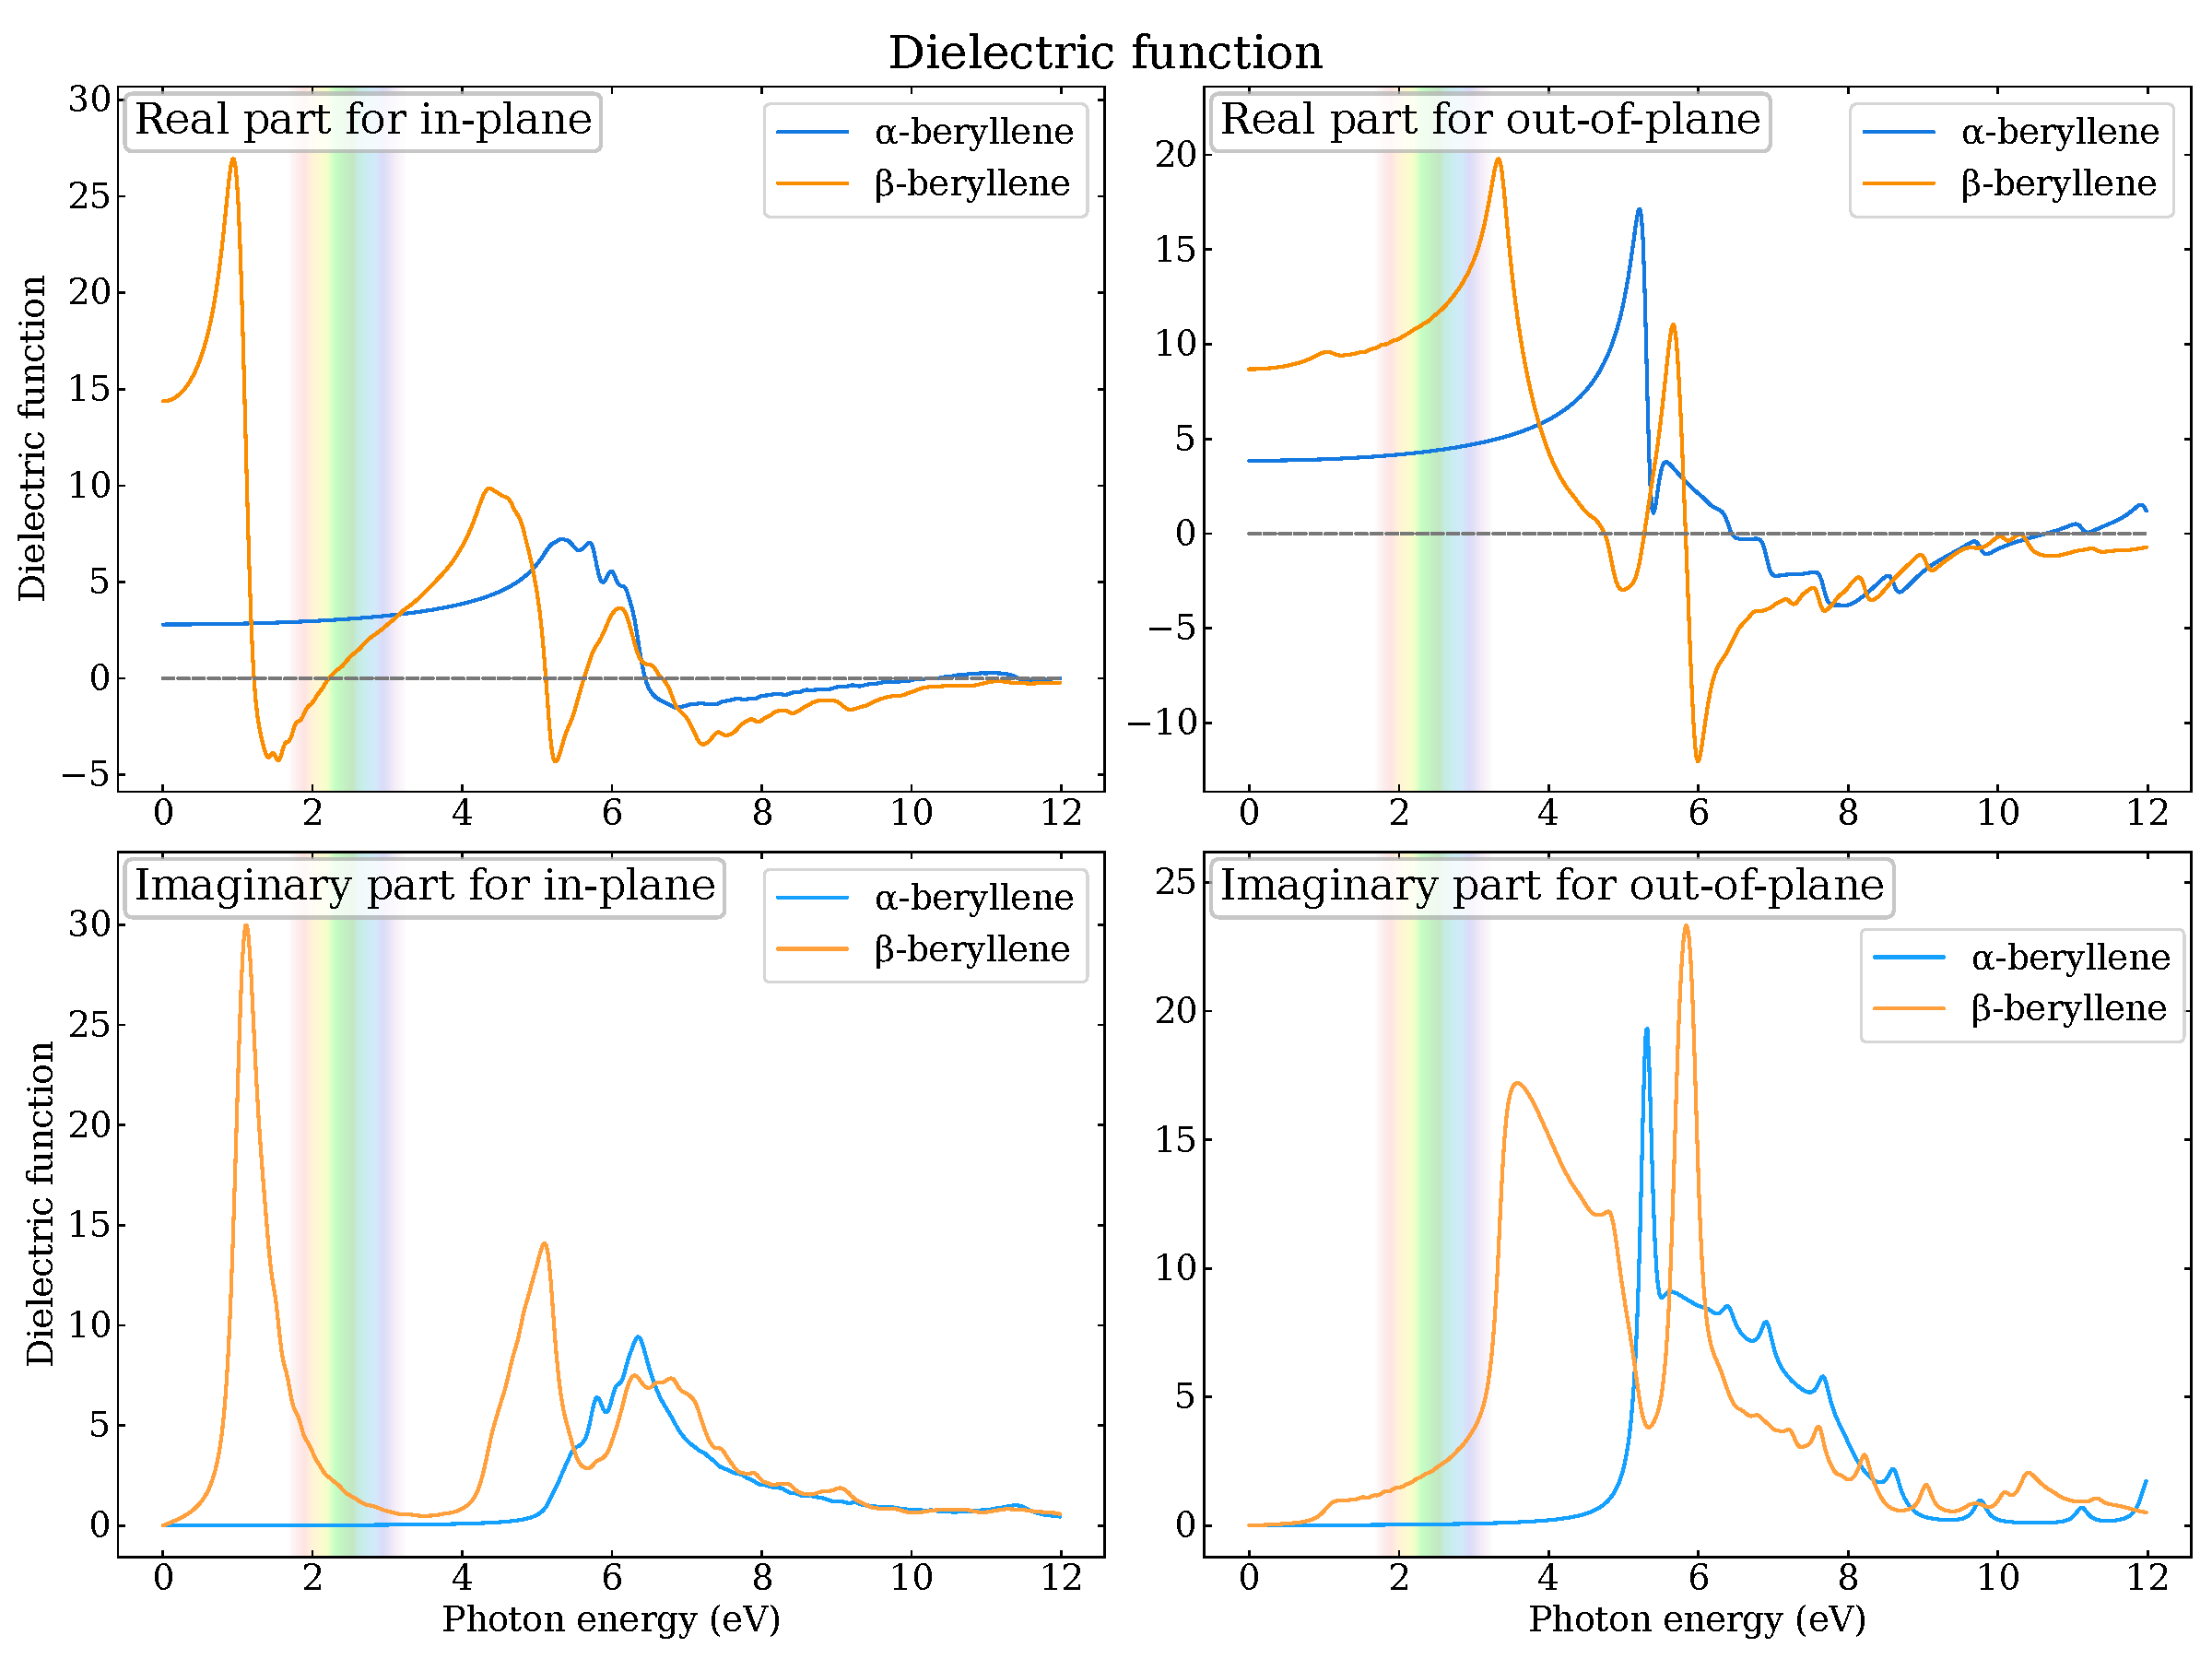
\includegraphics[width=0.95\textwidth]{figures_ch3/3.1_dielectric.pdf}
\caption{Representative real and imaginary parts of the in-plane and out-of-plane dielectric function as a function of photon energy for $\alpha$-beryllene and $\beta$-beryllene. The figure illustrates the direction-resolved complex dielectric response discussed in the text.
The in-plane and out-of-plane curves correspond to the $xx$ and $zz$ components, respectively.
These spectra are from our calculations presented in chapter~\ref{cha:project_beryllene}.}
\label{figure_representative_dielectric_response}
\end{figure}

At this stage, we have established the direction-resolved complex dielectric response for anisotropic media.
For each principal direction, the real and imaginary parts are not independent.
In the next section,
we introduce causality as the fundamental constraint on the linear response,
and then derive the Kramers--Kronig relations for each directional component.

\newpage
\section{Causality and the Kramers--Kronig relations}
\label{sec:causality_and_kramers_kronig_relations}

% opening paragraph
The previous section established a direction-resolved complex dielectric response for anisotropic media.
We now identify the constraint that connects the real and imaginary parts of each directional component.

Here, the major physical constraint is causality~\cite{toll1956causality}.
Specifically, causality means that the polarization response cannot occur before the external electric field is applied.
Equivalently, in the time domain, the response kernel vanishes when the response time precedes the driving time.
This temporal order determines the analytic structure of the response function in frequency space.
As a result, for each complex component,
the real and imaginary parts cannot vary independently;
instead, they are related through the Kramers--Kronig relations~\cite{de1926theory, toll1956causality, lucarini2005kramers}.

Therefore, for the dielectric response, once we calculate the absorptive part,
we can determine the dispersive part and construct the complete dielectric response.
This connection completes the dielectric response and opens the derivation of the optical properties.

\subsection{Kramers--Kronig relations for the dielectric function}

The analytic structure of the dielectric response is derived in section~\ref{sec:causality_derivation_basic} of appendix~\ref{cha:appendix_electrodynamics}.
We now use this causal structure to connect the real and imaginary parts of the dielectric function~\cite{toll1956causality}.
Here, we consider the regular electronic response without a zero-frequency conductivity pole,
with $\varepsilon_{\alpha\beta}(\omega)\to\delta_{\alpha\beta}$ at high frequency.
For a metal, the conductive term must be separated before applying these relations in the form below.
The dielectric function in this derivation then denotes the remaining regular response.

The symmetry relations in equation~\eqref{parity_of_dielectric_components} reduce the full-frequency integrals to positive-frequency integrals.
In the principal-axis representation,
each complex dielectric component $\varepsilon_{\lambda\lambda}(\omega)$ satisfies the Kramers--Kronig relations in the form~\cite{ossikovski2021constitutive}:

\begin{equation}
\left\{\begin{aligned}
    \varepsilon_{1,\lambda\lambda}(\omega) &=
    1+\frac{2}{\mathrm{\pi}}\mathcal{P}
    \int_{0}^{\infty}\dif{\omega'}\,
    \frac{\omega'\varepsilon_{2,\lambda\lambda}(\omega')}{\omega'^2-\omega^2} \\
    \varepsilon_{2,\lambda\lambda}(\omega) &=
    -\frac{2\omega}{\mathrm{\pi}}\mathcal{P}
    \int_{0}^{\infty}\dif{\omega'}\,
    \frac{\varepsilon_{1,\lambda\lambda}(\omega')-1}{\omega'^2-\omega^2}  
\end{aligned}\right.
\label{kk_positive_frequency_dielectric_component}
\end{equation}

here, $\mathcal{P}$ denotes the Cauchy principal value.

These relations provide the positive-frequency form of the dielectric response in the present work.
Once we obtain the absorptive part $\varepsilon_{2,\lambda\lambda}(\omega)$ from the electronic transitions,
equation~\eqref{kk_positive_frequency_dielectric_component} determines the dispersive part $\varepsilon_{1,\lambda\lambda}(\omega)$.
This relation also preserves the causal connection between the two parts of the dielectric response.

Consequently, the complex dielectric function describes the absorptive
and dispersive responses of the medium within a unified framework.
The imaginary part characterizes the energy absorbed by the medium at a given frequency,
whereas the real part describes the associated dispersion generated by the same response process.
Within this framework, equation~\eqref{kk_positive_frequency_dielectric_component} directly determines the static limit.
In the next subsection, we derive the corresponding static expression and clarify its physical meaning.

\subsection{Static limit and physical interpretation}

The previous subsection established the positive-frequency form of the Kramers--Kronig relations for the dielectric response.
We now describe the static limit and clarify its physical interpretation~\cite{onishi2024universal,vandenberghe2023two}.

Firstly, for the regular electronic response with a convergent static integral,
we set $\omega\to0$ in the positive-frequency Kramers--Kronig relations~\eqref{kk_positive_frequency_dielectric_component}.
This limit does not represent the full static dielectric response of a conducting system.
We then obtain the static electronic response in the principal-axis representation:

\begin{equation}
    \varepsilon_{1,\lambda\lambda}(0)
    = 1+\frac{2}{\mathrm{\pi}}
    \int_{0}^{\infty}\dif{\omega'}\,
    \frac{\varepsilon_{2,\lambda\lambda}(\omega')}{\omega'}
\label{static_limit_from_kramers_kronig}
\end{equation}

here, $\varepsilon_{1,\lambda\lambda}(0)$ characterizes the static dielectric response along the principal direction $\lambda$.
This expression shows that the static limit is not an independent quantity;
instead, the full directional absorption spectrum $\varepsilon_{2,\lambda\lambda}(\omega)$ determines it through causality~\cite{osanloo2021identification}.

Next, the factor $1/\omega'$ gives higher weight to low-energy spectral contributions.
The dominant contribution nevertheless depends on the spectral weight over the full energy range.
Therefore, the static limit represents an accumulated response over the full absorption spectrum.

Meanwhile, anisotropic media generally exhibit different spectral-weight distributions along different principal directions~\cite{suk2024ultrafast,sun2025recent}.

The Kramers--Kronig relations~\eqref{static_limit_from_kramers_kronig} describe a direct directional dependence in the static limit.
The different directional absorption spectra produce different directional static dielectric responses~\cite{suk2024ultrafast}.

Consequently, the static limit reveals the physical interpretation of the Kramers--Kronig relations.
The imaginary part characterizes the spectral weight generated by electronic excitations, 
whereas the real part determines the corresponding zero-frequency dielectric response.
Therefore, the complex dielectric function provides the complete information required for the subsequent optical properties~\cite{lucarini2005kramers,vandenberghe2023two}.

We next use the same dielectric response to derive the absorption coefficient, refractive index, extinction coefficient, reflectivity, and energy-loss spectrum.

\newpage
\section{From the dielectric function to optical properties}
\label{sec:from_dielectric_function_to_optical_properties}

% opening paragraph
The previous section established the complex dielectric function.
It describes the optical response of the present systems.
We now apply this dielectric response to determine the
corresponding optical properties.

We start from the absorption coefficient $\alpha(\omega)$,
which characterizes the attenuation of incident light in the
medium.
We then turn to the refractive index $n(\omega)$ and extinction
coefficient $k(\omega)$, which describe phase propagation and
amplitude decay.
Next, we determine the reflectivity $R(\omega)$, which
represents the reflected portion of the electromagnetic wave at
the interface.
Finally, we examine the energy-loss spectrum $L(\omega)$,
which identifies the dominant resonant energy-loss channels in the medium.

In what follows, we present the general relations that
connect these quantities to the complex dielectric function $\varepsilon(\omega)$~\cite{born2013principles,wooten2013optical,dressel2002electrodynamics,fox2010optical}.
Recent first-principles studies have also analysed the dielectric response together with the derived optical properties in low-dimensional materials~\cite{niu2024electronic,khan2025insight,albert2024optical,huang2023optical,cheng2025two}.
Afterwards, we analyse the in-plane and out-of-plane optical response of the present systems.
We will discuss the individual spectral features in detail in section~\ref{3_optical_alpha_beta}.
For absorption, refraction, and reflection, we use the local effective-medium description of a transverse principal-axis mode with $\mu_{\mathrm{r}}(\omega)\approx1$.
The index $\lambda$ denotes the electric-field polarization.
In the propagation equations, $z$ denotes distance along the wave path and need not coincide with the structural out-of-plane axis.

\subsection{Absorption coefficient}

We first consider the absorption coefficient $\alpha_{\lambda}(\omega)$,
which characterizes the optical attenuation for polarization along the principal direction $\lambda$~\cite{lin2023recent}.

For a monochromatic wave propagating through the medium,
the intensity follows:

\begin{equation}
    I_{\lambda}(z,\omega)= I_{\lambda,0}(\omega)\,\mathrm{e}^{-\alpha_{\lambda}(\omega) z}
\label{intensity_attenuation_from_absorption_coefficient}
\end{equation}

here, we use $z$ to represent the propagation distance in the medium.
$I_{\lambda,0}(\omega)$ is the intensity just inside the medium at $z=0$,
and $I_{\lambda}(z,\omega)$ is the intensity at depth $z$.
Therefore, a larger absorption coefficient corresponds to
stronger attenuation and shorter optical penetration depth.

We next introduce the complex refractive index along the
principal direction $\lambda$:

\begin{equation}
    N_{\lambda}(\omega) = n_{\lambda}(\omega) +\mathrm{i}\, k_{\lambda}(\omega)
\label{complex_refractive_index_for_absorption_coefficient}
\end{equation}

here, $n_{\lambda}(\omega)$ denotes the refractive index,
whereas $k_{\lambda}(\omega)$ denotes the extinction coefficient.
We then express the absorption coefficient $\alpha_{\lambda}(\omega)$ as:

\begin{equation}
    \alpha_{\lambda}(\omega)
    = \frac{2\,\omega}{c}k_{\lambda}(\omega)
\label{absorption_coefficient_from_extinction_coefficient}
\end{equation}

here, $c$ is the speed of light in vacuum.
This expression connects the absorption coefficient to the imaginary part of the complex refractive index.
That imaginary part drives the amplitude decay in the medium~\cite{wooten2013optical, dressel2002electrodynamics,fox2010optical,gajdovs2006linear}.

We now combine the defining relation between the complex
refractive index $N_{\lambda}(\omega)$
and the complex dielectric function $\varepsilon_{\lambda\lambda}(\omega)$ as~\cite{born2013principles}:

\begin{equation}
    N_{\lambda}^{2}(\omega)= \varepsilon_{\lambda\lambda}(\omega)
\label{refractive_index_dielectric_relation}
\end{equation}

Using this relation together with equation~\eqref{direction_resolved_complex_dielectric_function},
we then derive the absorption coefficient $\alpha_{\lambda}(\omega)$ from the complex dielectric function $\varepsilon_{\lambda\lambda}(\omega)$~\cite{born2013principles}:

\begin{equation}
    \alpha_{\lambda}(\omega)
    = \frac{\sqrt{2}\,\omega}{c}
    \left[\sqrt{\varepsilon_{1,\lambda\lambda}^{2}(\omega)
        + \varepsilon_{2,\lambda\lambda}^{2}(\omega)}
        - \varepsilon_{1,\lambda\lambda}(\omega)\right]^{1/2}
\label{absorption_coefficient_from_dielectric_function}
\end{equation}

This equation expresses the absorption coefficient as a
response quantity derived from the dielectric function.
Here, the imaginary part $\varepsilon_{2,\lambda\lambda}(\omega)$ provides the spectral weight generated by electronic transitions,
whereas the real part $\varepsilon_{1,\lambda\lambda}(\omega)$ modifies the magnitude and energy dependence of the resulting attenuation.

Figure~\ref{absorption_coefficient_present_systems} presents the calculated absorption coefficient $\alpha_{\lambda}(\omega)$ spectra of the present systems for the in-plane and out-of-plane directions.

\begin{figure}[htbp]
\centering
    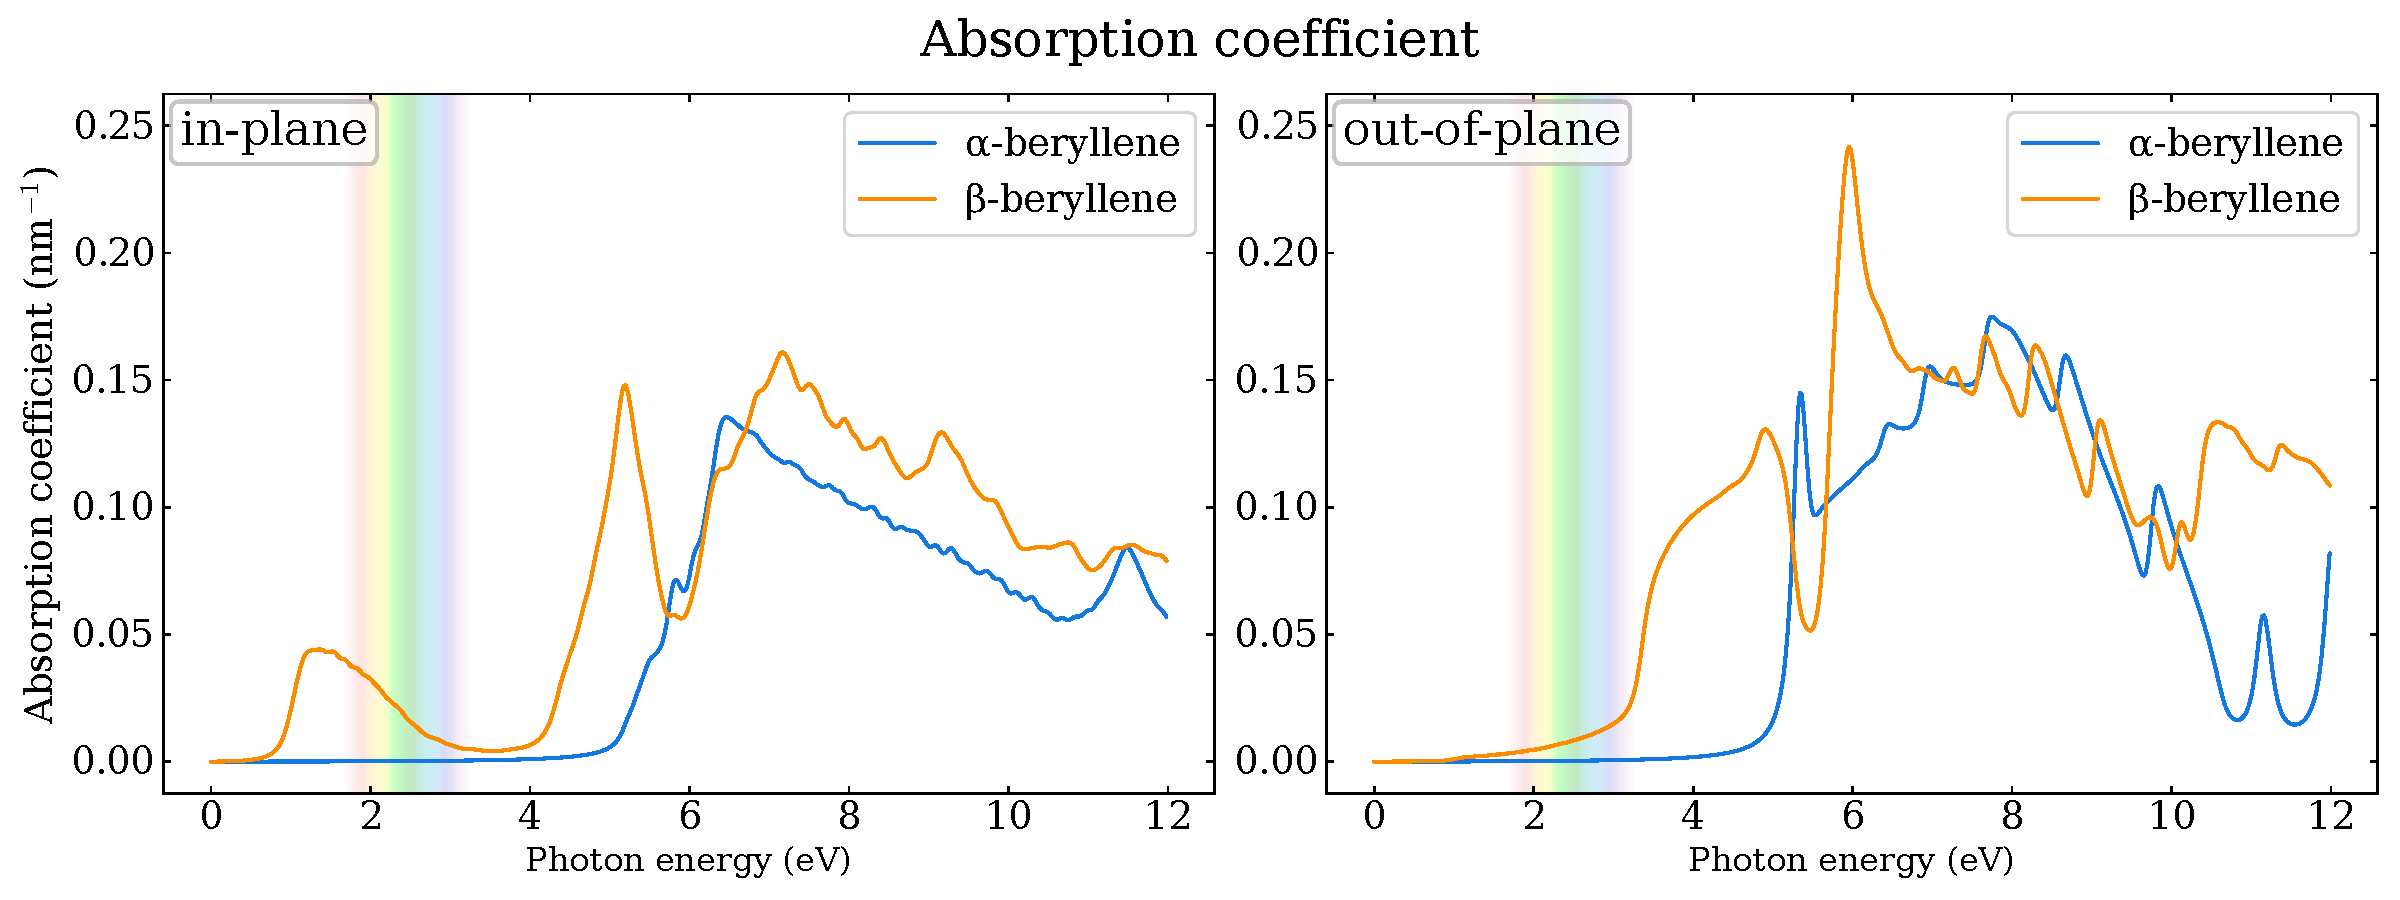
\includegraphics[width=0.95\textwidth]{figures_ch3/4.1_absorption.pdf}
\caption{The absorption coefficients for the in-plane and out-of-plane directions as functions of photon energy for $\alpha$-beryllene and $\beta$-beryllene.
The in-plane and out-of-plane curves correspond to the $xx$ and $zz$ components, respectively. The absorption coefficient is given in $\mathrm{nm}^{-1}$.
These spectra are from our calculations presented in chapter~\ref{cha:project_beryllene}.}
\label{absorption_coefficient_present_systems}
\end{figure}

The absorption coefficient spectra demonstrate differences between the two optical directions and between the two materials.
These trends indicate that the optical attenuation depends on both the polarization direction and the crystal structure of the medium.

Once the electronic transitions generate different spectral weights along different directions,
the corresponding optical attenuation also acquires directional dependence~\cite{suk2024ultrafast}.

The low-energy increase of $\alpha_{\lambda}(\omega)$ identifies the beginning of the optical transitions.
As the photon energy increases, broader peaks emerge in the absorption spectrum.
These peaks indicate energy ranges where interband transitions contribute more strongly to the absorption process~\cite{elbanna20232d}.

Therefore, the absorption coefficient $\alpha_{\lambda}(\omega)$ reflects the directional excitation spectrum of the medium and characterizes the rate of optical attenuation~\cite{niu2024electronic,khan2025insight,zhang2024advanced,elbanna20232d}.
We next apply the same dielectric response to determine the refractive index $n_{\lambda}(\omega)$ and extinction coefficient $k_{\lambda}(\omega)$,
which describe the propagation of the attenuated wave.

\subsection{Refractive index and extinction coefficient}

The previous subsection described the absorption coefficient as the optical quantity that characterizes energy dissipation in the medium.
We now continue this description of light propagation in the medium by introducing the refractive index $n_{\lambda}(\omega)$ and the extinction coefficient $k_{\lambda}(\omega)$.
The refractive index determines the phase evolution,
whereas the extinction coefficient describes the attenuation of the wave amplitude.
Starting from the dielectric response,
we derive explicit expressions for $n_{\lambda}(\omega)$ and $k_{\lambda}(\omega)$~\cite{born2013principles,wooten2013optical,dressel2002electrodynamics,fox2010optical}.

For a monochromatic transverse mode polarized along the principal direction $\lambda$,
we first represent the electric field along the propagation coordinate $z$ as~\cite{politano2023spectroscopic}:

\begin{equation}
\begin{aligned}
    E_{\lambda}(z,t)
    &= E_{\lambda,0}\,
    \exp\left[\mathrm{i}\frac{\omega}{c}N_{\lambda}(\omega)z-\mathrm{i}\,\omega t\right]\\
    &= E_{\lambda,0}\,
    \exp\left[\mathrm{i}\frac{\omega}{c}n_{\lambda}(\omega)z\right]
    \exp\left[-\frac{\omega}{c}k_{\lambda}(\omega)z\right]
    \exp\left(-\mathrm{i}\,\omega t\right)
\end{aligned}
\label{monochromatic_wave_with_complex_refractive_index}
\end{equation}

here, $N_{\lambda}(\omega)$ denotes the complex refractive index.
Its real part $n_{\lambda}(\omega)$ denotes the refractive index,
and its imaginary part $k_{\lambda}(\omega)$ denotes the extinction coefficient.

This expression separates phase evolution from amplitude attenuation~\cite{wooten2013optical,dressel2002electrodynamics,born2013principles}.
In equation~\eqref{monochromatic_wave_with_complex_refractive_index},
the refractive index $n_{\lambda}(\omega)$ determines the phase evolution of the electromagnetic wave,
whereas the extinction coefficient $k_{\lambda}(\omega)$ describes the exponential attenuation of its amplitude in the medium.

For this mode and a scalar relative magnetic permeability $\mu_{\mathrm{r}}(\omega)$,
we write the relation between the complex refractive index and dielectric function as~\cite{born2013principles,wooten2013optical,dressel2002electrodynamics,politano2023spectroscopic}:

\begin{equation}
    N_{\lambda}^{2}(\omega)
    = \varepsilon_{\lambda\lambda}(\omega)\,\mu_{\mathrm{r}}(\omega)
\label{general_refractive_index_permeability_relation}
\end{equation}

here, $\mu_{\mathrm{r}}(\omega)$ is dimensionless.
Under the optical approximation $\mu_{\mathrm{r}}(\omega)\approx1$,
the relation reduces to~\cite{wooten2013optical,dressel2002electrodynamics,born2013principles}:

\begin{equation}
    N_{\lambda}^{2}(\omega)
    = \varepsilon_{\lambda\lambda}(\omega)
\label{nonmagnetic_refractive_index_dielectric_relation}
\end{equation}

We substitute equation~\eqref{direction_resolved_complex_dielectric_function}
and the definition of the complex refractive index $N_{\lambda}(\omega)$ in equation~\eqref{complex_refractive_index_for_absorption_coefficient}
into equation~\eqref{nonmagnetic_refractive_index_dielectric_relation},
and then separate the real and imaginary parts.
We therefore derive the coupled relations~\cite{wooten2013optical,dressel2002electrodynamics,fox2010optical}:

\begin{equation}
\begin{aligned}
    n_{\lambda}^{2}(\omega)-k_{\lambda}^{2}(\omega)
    &= \varepsilon_{1,\lambda\lambda}(\omega) \\
    2\,n_{\lambda}(\omega)\,k_{\lambda}(\omega)
    &= \varepsilon_{2,\lambda\lambda}(\omega)
\end{aligned}
\label{refractive_index_extinction_coefficient_auxiliary_relations}
\end{equation}

These two equations connect the refractive index $n_{\lambda}(\omega)$ and extinction coefficient $k_{\lambda}(\omega)$ to the real part $\varepsilon_{1,\lambda\lambda}(\omega)$ and imaginary part $\varepsilon_{2,\lambda\lambda}(\omega)$ of the dielectric function $\varepsilon_{\lambda\lambda}(\omega)$.

By solving these coupled relations,
we express the refractive index $n_{\lambda}(\omega)$ as~\cite{capper2019optical,cheng2025two,kim2024hyperspectral}:

\begin{equation}
    n_{\lambda}(\omega) = 
    \left[\frac{1}{2}\left(\sqrt{\varepsilon_{1,\lambda\lambda}^{2}(\omega)
        + \varepsilon_{2,\lambda\lambda}^{2}(\omega)}
        + \varepsilon_{1,\lambda\lambda}(\omega)\right)\right]^{1/2}
\label{refractive_index_from_dielectric_response}
\end{equation}

Similarly, we express the extinction coefficient $k_{\lambda}(\omega)$ as:

\begin{equation}
    k_{\lambda}(\omega) =
    \left[\frac{1}{2}\left(\sqrt{\varepsilon_{1,\lambda\lambda}^{2}(\omega)
        + \varepsilon_{2,\lambda\lambda}^{2}(\omega)}
        - \varepsilon_{1,\lambda\lambda}(\omega)\right)\right]^{1/2}
\label{extinction_coefficient_from_dielectric_response}
\end{equation}

With these expressions, we present the calculated refractive index $n_{\lambda}(\omega)$ spectra of $\alpha$-beryllene and $\beta$-beryllene in figure~\ref{refractive_index_present_systems}.

\begin{figure}[htbp]
\centering
    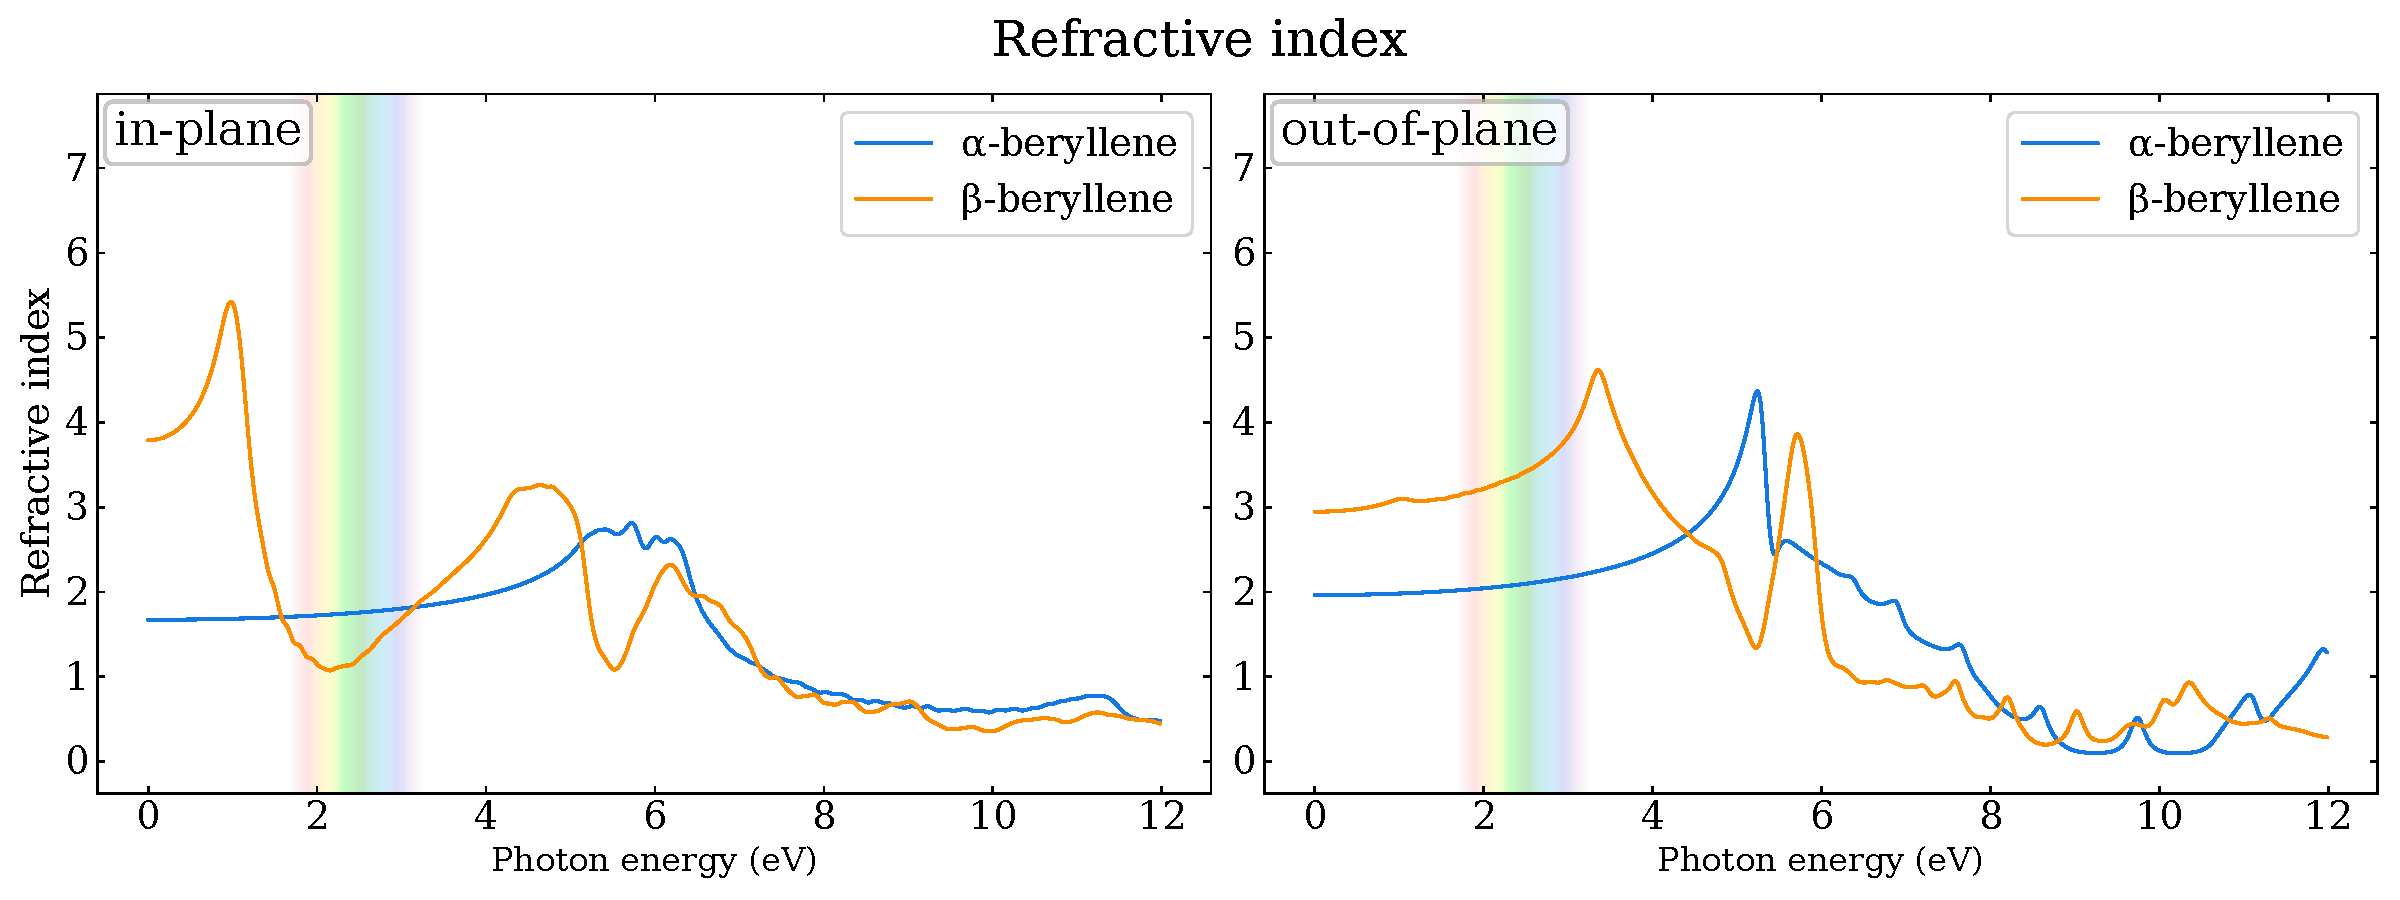
\includegraphics[width=0.95\textwidth]{figures_ch3/4.2_refractive.pdf}
\caption{The refractive indices for the in-plane and out-of-plane directions as functions of photon energy for $\alpha$-beryllene and $\beta$-beryllene.
The in-plane and out-of-plane curves correspond to the $xx$ and $zz$ components, respectively.
These spectra are from our calculations presented in chapter~\ref{cha:project_beryllene}.}
\label{refractive_index_present_systems}
\end{figure}

The refractive index spectra demonstrate distinct directional and structural contrasts.
These trends indicate that the phase response depends on both the optical direction and the crystal structure of the medium.

We next present the extinction coefficient $k_{\lambda}(\omega)$ spectra in figure~\ref{extinction_coefficient_alpha_beta_beryllene},
which follow the absorptive part of the dielectric response more directly~\cite{wooten2013optical,dressel2002electrodynamics,fox2010optical}.

\begin{figure}[htbp]
\centering
    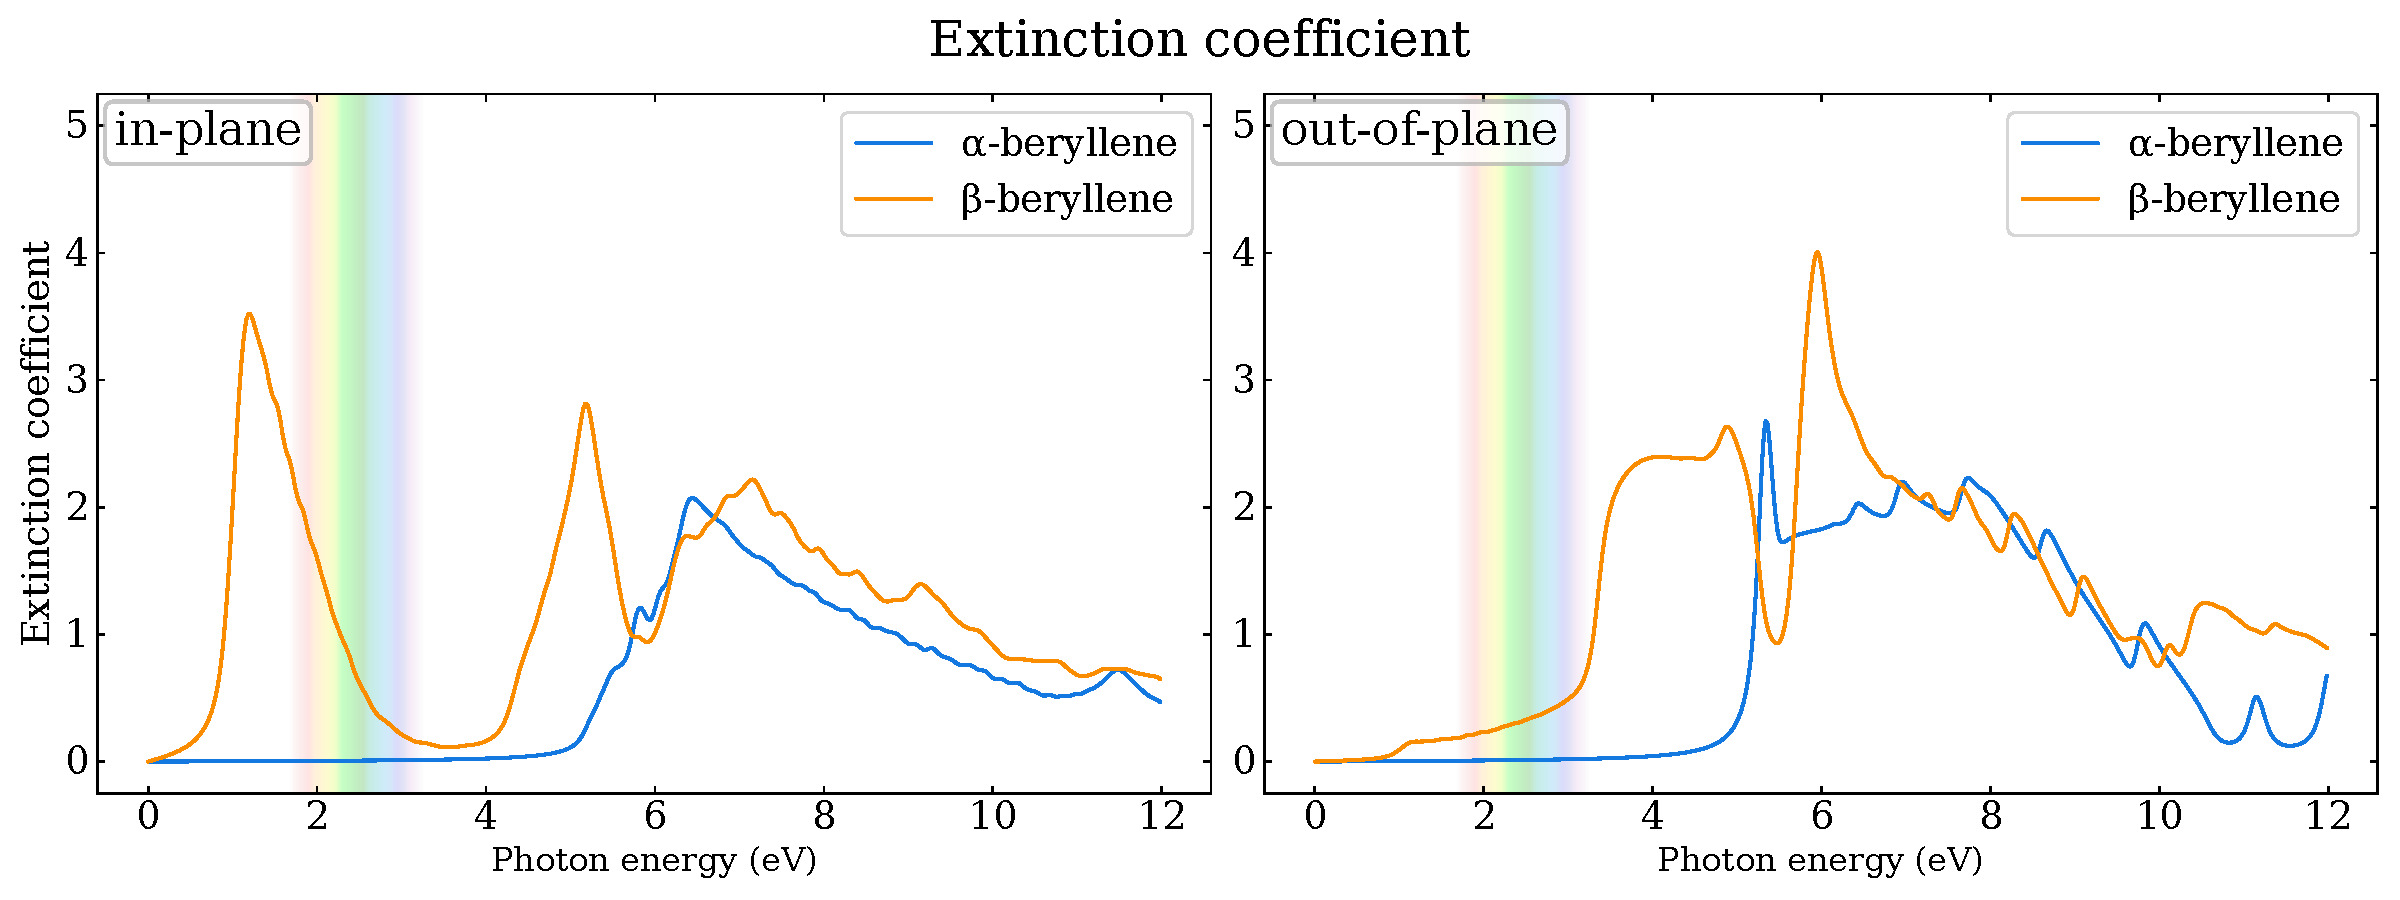
\includegraphics[width=0.95\textwidth]{figures_ch3/4.3_extinction.pdf}
\caption{The extinction coefficients for the in-plane and out-of-plane directions as functions of photon energy for $\alpha$-beryllene and $\beta$-beryllene.
The in-plane and out-of-plane curves correspond to the $xx$ and $zz$ components, respectively.
These spectra are from our calculations presented in chapter~\ref{cha:project_beryllene}.}
\label{extinction_coefficient_alpha_beta_beryllene}
\end{figure}

The extinction coefficient spectra demonstrate a similar directional contrast.
This behaviour shows that amplitude attenuation also depends on both the optical direction and the crystal structure of the medium.

Accordingly, the refractive index $n_{\lambda}(\omega)$ and extinction coefficient $k_{\lambda}(\omega)$ connect the dielectric function to the interface response through the Fresnel equations~\cite{born2013principles,wooten2013optical,dressel2002electrodynamics}.
We next use them to determine the reflectivity, which transfers the bulk optical response to the interface.

\subsection{Reflectivity}

The previous subsection determined the refractive index $n_{\lambda}(\omega)$ and extinction coefficient $k_{\lambda}(\omega)$,
which characterize the phase propagation and amplitude attenuation in the medium.
We now turn from propagation inside the medium to reflection at its surface.

The reflectivity $R_{\lambda}(\omega)$ characterizes the fraction of incident electromagnetic energy reflected at the interface.
We then describe it through the Fresnel coefficient at normal incidence~\cite{born2013principles,wooten2013optical,dressel2002electrodynamics,fox2010optical}.

When an electromagnetic wave reaches the interface between two media,
the mismatch of optical response generates a reflected wave and a transmitted wave.
For a plane wave incident from an ambient medium with complex refractive index $N_{0,\lambda}(\omega)$ onto the present system with complex refractive index $N_{\lambda}(\omega)$,
the amplitude reflection coefficient at normal incidence takes the general form~\cite{born2013principles,wooten2013optical}:

\begin{equation}
    r_{\lambda}(\omega) =
    \frac{N_{\lambda}(\omega)-N_{0,\lambda}(\omega)}
    {N_{\lambda}(\omega)+N_{0,\lambda}(\omega)}
\label{normal_incidence_amplitude_reflection_coefficient_general}
\end{equation}

here, $r_{\lambda}(\omega)$ denotes the amplitude reflection coefficient,
$N_{0,\lambda}(\omega)$ denotes the complex refractive index of the incident medium,
and $N_{\lambda}(\omega)$ denotes the complex refractive index of the present medium.

For the optical quantities derived here,
we consider an interface between vacuum and a homogeneous semi-infinite effective medium with $\mu_{\mathrm{r}}(\omega)\approx1$.
The incident medium therefore satisfies $N_{0,\lambda}(\omega)=1$.
The resulting reflectivity is a parameter of this effective-medium model.
For a finite two-dimensional layer, the measured reflectance also depends on the thickness, substrate, and optical geometry.
At normal incidence on the structural plane, the electric field is in-plane.
The value obtained from $\varepsilon_{zz}(\omega)$ is therefore a formal out-of-plane response of the scalar model.
With the complex refractive index $N_{\lambda}(\omega)$ in equation~\eqref{complex_refractive_index_for_absorption_coefficient},
we then write the amplitude reflection coefficient as:

\begin{equation}
    r_{\lambda}(\omega) =
    \frac{n_{\lambda}(\omega)-1+\mathrm{i}\,k_{\lambda}(\omega)}
    {n_{\lambda}(\omega)+1+\mathrm{i}\,k_{\lambda}(\omega)}
\label{normal_incidence_amplitude_reflection_coefficient_vacuum_interface}
\end{equation}

here, the refractive index $n_{\lambda}(\omega)$ determines the phase mismatch across the interface,
whereas the extinction coefficient $k_{\lambda}(\omega)$ represents the dissipative part of the optical response.
These two quantities together determine the reflected amplitude at the surface.

We next express the reflectivity $R_{\lambda}(\omega)$ as the reflected power ratio.
It equals the squared modulus of the amplitude reflection coefficient~\cite{born2013principles,wooten2013optical,dressel2002electrodynamics}:

\begin{equation}
    R_{\lambda}(\omega)
    = \left|r_{\lambda}(\omega)\right|^2
\label{reflectivity_from_amplitude_reflection_coefficient}
\end{equation}

After substituting equation~\eqref{normal_incidence_amplitude_reflection_coefficient_vacuum_interface},
this equation produces the reflectivity through the refractive index $n_\lambda(\omega)$ and the extinction coefficient $k_\lambda(\omega)$:

\begin{equation}
    R_{\lambda}(\omega) =
    \frac{\left[n_\lambda(\omega)-1\right]^2+k_\lambda^2(\omega)}
    {\left[n_\lambda(\omega)+1\right]^2+k_\lambda^2(\omega)}
\label{reflectivity_from_refractive_index_and_extinction_coefficient}
\end{equation}

This equation links the surface reflection to the refractive index $n_{\lambda}(\omega)$ and the extinction coefficient $k_{\lambda}(\omega)$.
A larger mismatch between $n_{\lambda}(\omega)$ and the vacuum value enhances reflection,
whereas $k_{\lambda}(\omega)$ modifies the reflected intensity through optical dissipation.
Therefore, the reflectivity $R_{\lambda}(\omega)$ characterizes the reflected optical response at a specific photon energy.

Figure~\ref{reflectivity_alpha_beta_beryllene} presents the calculated reflectivity $R_{\lambda}(\omega)$ spectra of $\alpha$-beryllene and $\beta$-beryllene for the in-plane and out-of-plane directions.

\begin{figure}[htbp]
\centering
    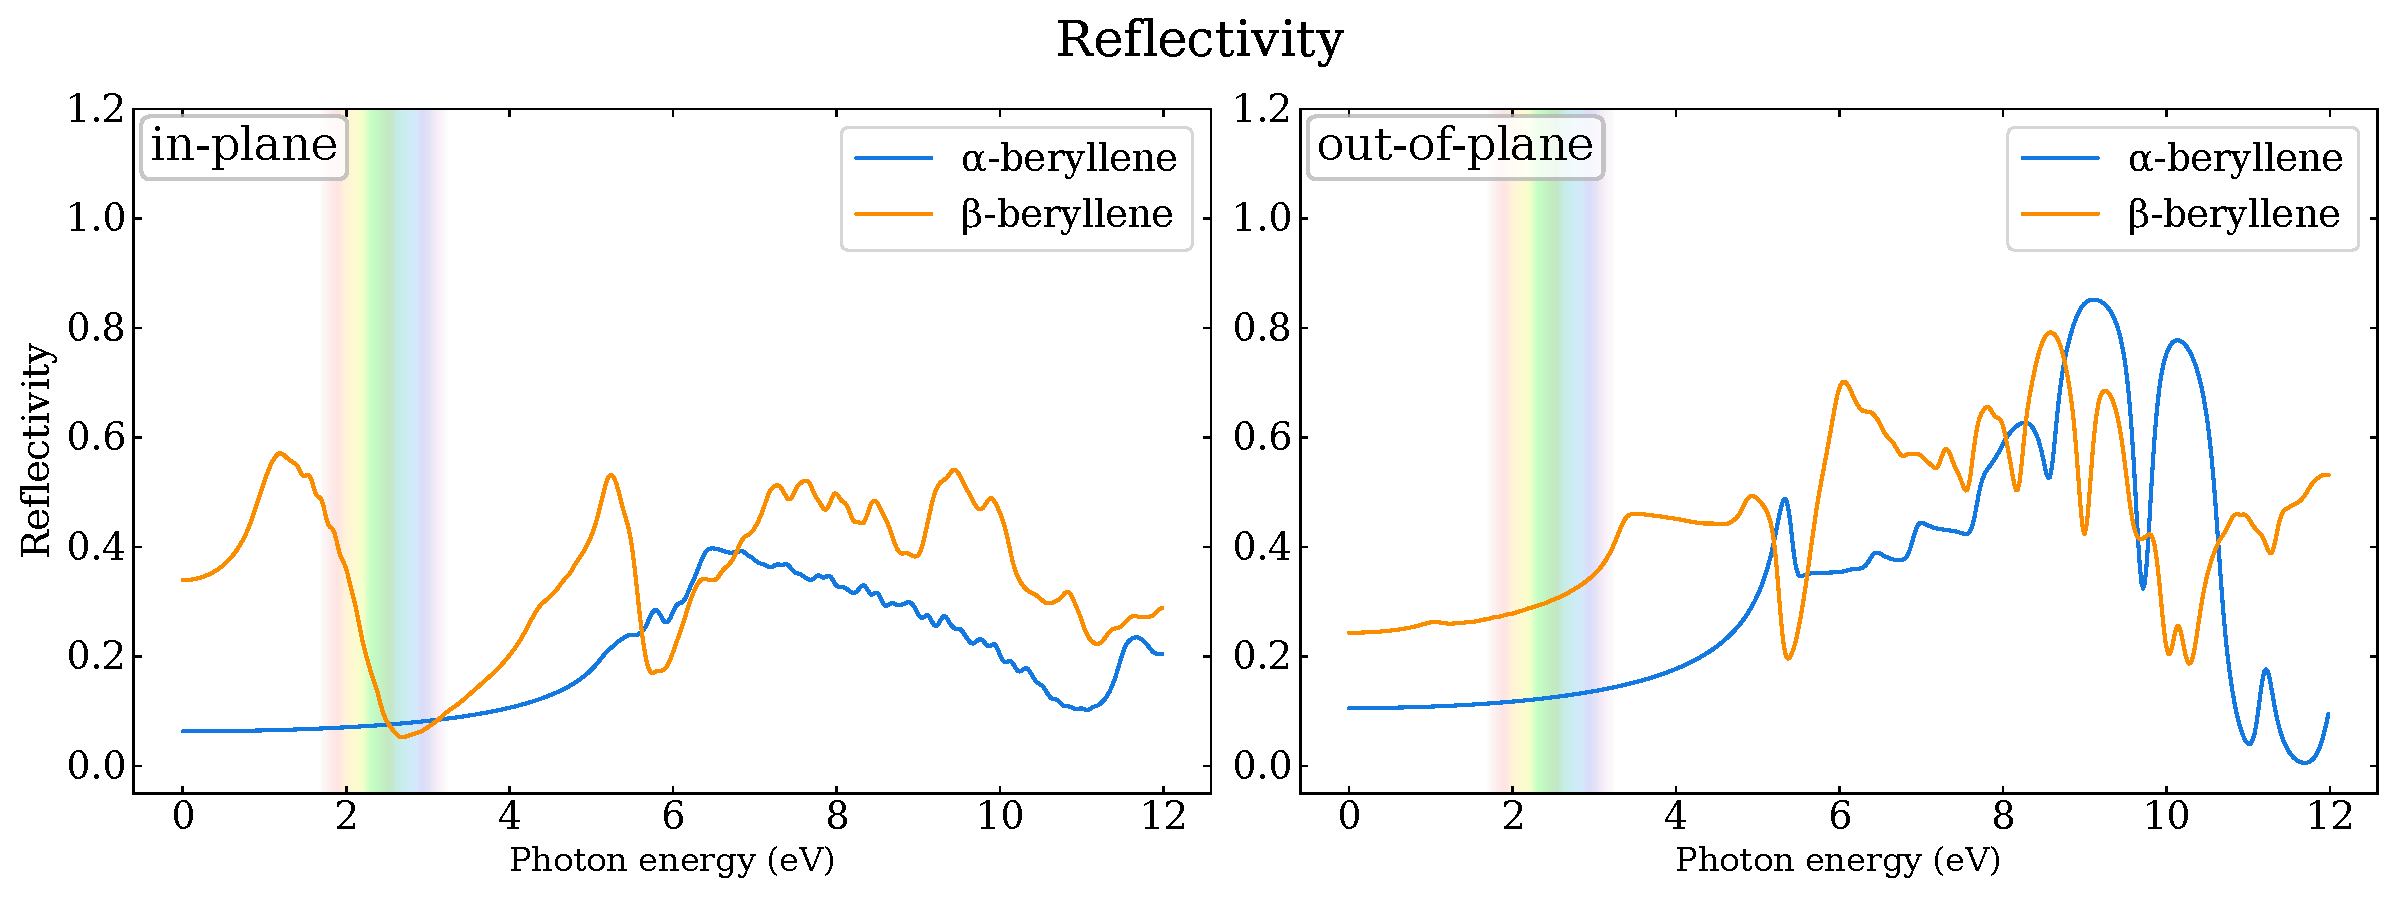
\includegraphics[width=0.95\textwidth]{figures_ch3/4.4_reflectivity.pdf}
\caption{The reflectivities for the in-plane and out-of-plane directions as functions of photon energy for $\alpha$-beryllene and $\beta$-beryllene.
The in-plane and out-of-plane curves correspond to the $xx$ and $zz$ components, respectively. The reflectivities are evaluated within the effective-medium model described in the text.
These spectra are from our calculations presented in chapter~\ref{cha:project_beryllene}.}
\label{reflectivity_alpha_beta_beryllene}
\end{figure}

The reflectivity spectra follow the directional contrast already demonstrated in the extinction coefficient.
These trends reflect the combined role of the refractive index $n_{\lambda}(\omega)$ and the extinction coefficient $k_{\lambda}(\omega)$ in determining the surface reflectivity.

We next turn to the energy-loss spectrum $L_{\lambda}(\omega)$ and examine the longitudinal loss response of the medium.

\subsection{Energy-loss spectrum}

The previous subsection introduced the reflectivity $R_{\lambda}(\omega)$ as the optical response of the surface,
characterized by the refractive index $n_{\lambda}(\omega)$ and the extinction coefficient $k_{\lambda}(\omega)$.
We now move from surface reflection to energy dissipation inside the medium by examining the energy-loss spectrum $L_{\lambda}(\omega)$.

The energy-loss spectrum $L_{\lambda}(\omega)$ characterizes the energy transferred from an external probe to the medium at an energy transfer $\hbar\omega$.
Here, we consider a longitudinal perturbation along the principal direction $\lambda$ in the local, long-wavelength limit.
This loss function describes the corresponding bulk response relevant to electron energy-loss spectroscopy~\cite{egerton2009electron,yao2025study}.
Finite momentum and surface contributions depend on the scattering geometry.

We first express this principal-axis energy-loss function as~\cite{dressel2002electrodynamics,wooten2013optical,fox2010optical,onida2002electronic}:

\begin{equation}
    L_{\lambda}(\omega)=
    \mathrm{Im}\left[-\frac{1}{\varepsilon_{\lambda\lambda}(\omega)}\right]
\label{energy_loss_spectrum_from_inverse_dielectric_function}
\end{equation}

This expression indicates that the energy-loss spectrum $L_{\lambda}(\omega)$ is governed by the inverse dielectric function $1/\varepsilon_{\lambda\lambda}(\omega)$.
For a medium, it therefore follows not only the imaginary part $\varepsilon_{2,\lambda\lambda}(\omega)$,
but also the screening effect determined by the full complex dielectric function $\varepsilon_{\lambda\lambda}(\omega)$.

For a weakly damped longitudinal collective excitation,
an energy-loss peak can occur near a zero of $\varepsilon_{1,\lambda\lambda}(\omega)$ when $\varepsilon_{2,\lambda\lambda}(\omega)$ is small.
Interband excitations also contribute to the energy-loss spectrum,
so a plasmon assignment combines an energy-loss peak with the zero of $\varepsilon_{1,\lambda\lambda}(\omega)$~\cite{dressel2002electrodynamics,onida2002electronic}.

Substituting equation~\eqref{direction_resolved_complex_dielectric_function} into equation~\eqref{energy_loss_spectrum_from_inverse_dielectric_function}, we then obtain the explicit expression adopted in the present work:

\begin{equation}
    L_{\lambda}(\omega) =
    \frac{\varepsilon_{2,\lambda\lambda}(\omega)}
    {\varepsilon_{1,\lambda\lambda}^{2}(\omega)
    + \varepsilon_{2,\lambda\lambda}^{2}(\omega)}
\label{energy_loss_spectrum_from_dielectric_function}
\end{equation}

This expression separates the dissipative channel from the dielectric screening.
The imaginary part $\varepsilon_{2,\lambda\lambda}(\omega)$ enters both the numerator and the denominator.
At $\varepsilon_{1,\lambda\lambda}(\omega)=0$ and finite positive $\varepsilon_{2,\lambda\lambda}(\omega)$,
the energy-loss function is $L_{\lambda}(\omega)=1/\varepsilon_{2,\lambda\lambda}(\omega)$.
Therefore, a larger imaginary part lowers the energy-loss peak at the zero crossing.
The energy-loss spectrum describes longitudinal screening and complements the transverse absorption and reflection responses~\cite{dressel2002electrodynamics,onida2002electronic}.

Figure~\ref{energy_loss_spectrum_alpha_beta_beryllene} presents the calculated energy-loss $L_{\lambda}(\omega)$ spectra of $\alpha$-beryllene and $\beta$-beryllene for the in-plane and out-of-plane directions.

\begin{figure}[htbp]
\centering
    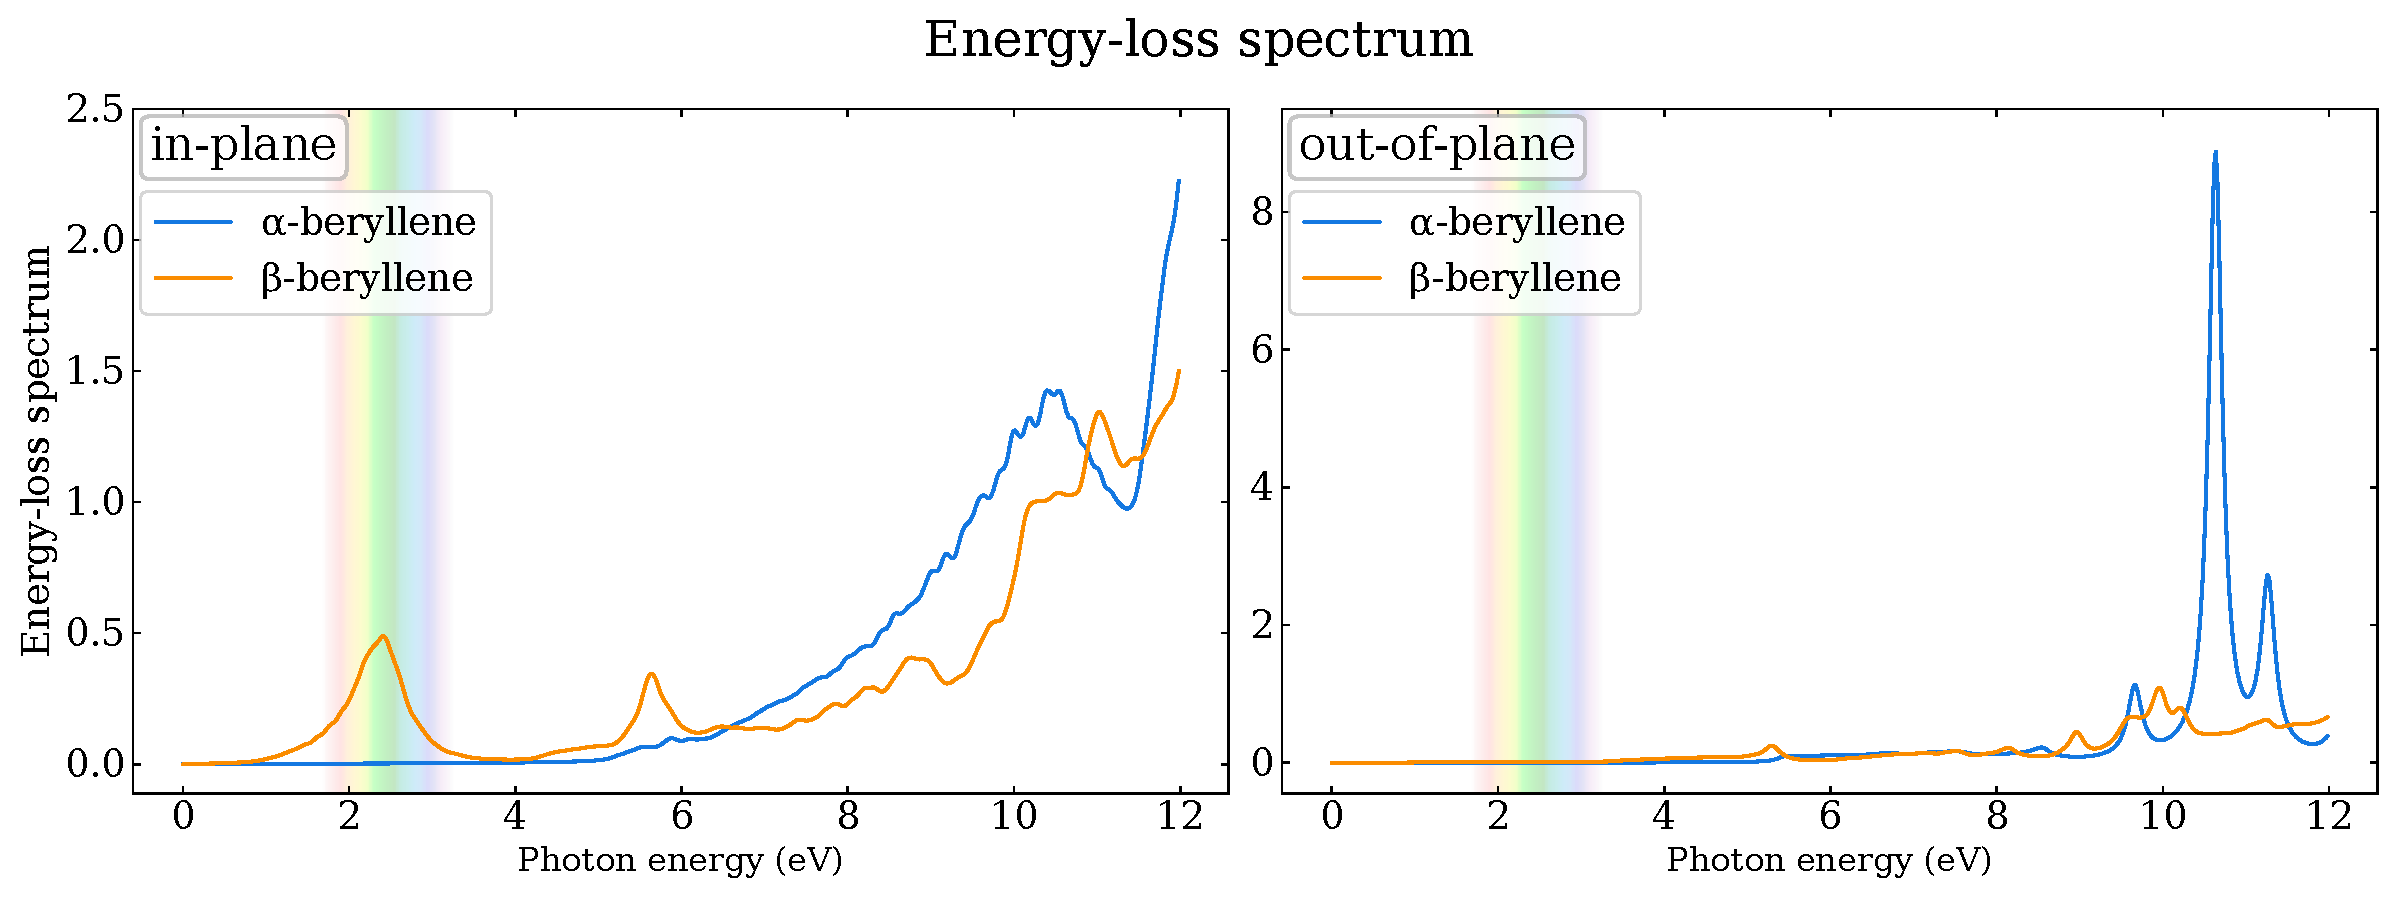
\includegraphics[width=0.95\textwidth]{figures_ch3/4.5_energy-loss.pdf}
\caption{The energy-loss spectra for the in-plane and out-of-plane directions as functions of photon energy for $\alpha$-beryllene and $\beta$-beryllene.
The in-plane and out-of-plane curves correspond to the $xx$ and $zz$ components, respectively.
These spectra are from our calculations presented in chapter~\ref{cha:project_beryllene}.}
\label{energy_loss_spectrum_alpha_beta_beryllene}
\end{figure}

The energy-loss spectra demonstrate clear directional and structural contrasts.
These results demonstrate that the energy-loss spectrum $L_{\lambda}(\omega)$ varies with both the response direction and the crystal structure of the medium.
As $L_{\lambda}(\omega)$ follows the inverse dielectric function,
its peaks identify energy ranges with a strong longitudinal energy-loss response.

Consequently, we arrive at the final optical quantity derived from the dielectric function $\varepsilon_{\lambda\lambda}(\omega)$ and complete the chain from the absorption coefficient $\alpha_{\lambda}(\omega)$,
to the refractive index $n_{\lambda}(\omega)$ and extinction coefficient $k_{\lambda}(\omega)$, to the reflectivity $R_{\lambda}(\omega)$, and finally to the energy-loss spectrum $L_{\lambda}(\omega)$.

\cleardoublepage
\chapter{Fundamentals \textRoman{3}: Band Topology}
\label{cha:fundamentals_c}

% opening paragraph
We continue our discussion of the fundamentals in this chapter, where we introduce the topology of electronic bands.
Chapter~\ref{cha:fundamentals_a} established the electronic states and their energies within the Kohn--Sham framework.
Chapter~\ref{cha:fundamentals_b} then connected these states to the optical response through transition matrix elements and energy differences.
We now examine another property of the same electronic states, namely how they can be connected continuously across the Brillouin zone while preserving the symmetries of the system.
This connection carries information beyond the band energies~\cite{bansil2016colloquium}.

The discussion follows the parity analysis used for the beryllene systems in chapter~\ref{cha:project_beryllene}.
The geometric phase and the general action of time reversal are developed in appendix~\ref{cha:appendix_topology}.
Here, we start from the spinor Bloch states supplied by the electronic-structure calculation
and identify the band subspace to which a topological index can be assigned.
We then locate the time-reversal invariant momenta and determine how inversion acts on the Kramers pairs.
Finally, we use their parity eigenvalues to obtain the two-dimensional $\mathbb{Z}_2$ index and connect its interpretation to the calculated band structure.
Throughout this discussion, we distinguish the topology of a selected band subspace from an insulating state at the Fermi level.
This distinction is required when interpreting the metallic systems considered in the present work.

\newpage
\section{Towards the topology of Bloch states}
\label{sec:toward_band_topology}

% opening paragraph
In the previous two chapters, we used the electronic states to describe two different problems.
For the ground-state problem, we determined the states that reproduce the electron density.
For the optical problem, we examined how an external field induces transitions between these states.
The topological problem instead compares states at different wave vectors.
Before making this comparison, we therefore need to identify both the states and the subspace that they form.

\subsection{From band energies to electronic states}
\label{subsec:method_topology}

We begin with the Bloch representation introduced in equation~\eqref{bloch_state_cell_periodic_method}.
For a periodic one-particle hamiltonian $\hat{h}$, we write:

\begin{equation}
\left\{\begin{aligned}
    \ket{\psi_{n\vec{k}}}
    &=\mathrm{e}^{\mathrm{i}\vec{k}\cdot\hat{\vec{r}}}\ket{u_{n\vec{k}}} \\
    \hat{h}(\vec{k}\,)
    &\coloneqq\mathrm{e}^{-\mathrm{i}\vec{k}\cdot\hat{\vec{r}}}
    \hat{h}\,\mathrm{e}^{\mathrm{i}\vec{k}\cdot\hat{\vec{r}}} \\
    \hat{h}(\vec{k}\,)\ket{u_{n\vec{k}}}
    &=E_{n\vec{k}}\ket{u_{n\vec{k}}}
\end{aligned}\right.
\label{bloch_hamiltonian_topology}
\end{equation}

here, $n$ denotes the band index, $\vec{k}$ denotes the crystal wave vector,
and $\hat{\vec{r}}$ is the position operator.
The crystal momentum associated with $\vec{k}$ is $\hbar\vec{k}$.
The state $\ket{u_{n\vec{k}}}$ is the cell-periodic part of the Bloch state,
normalized over one unit cell as in chapter~\ref{cha:fundamentals_a}.
In this chapter, inner products between cell-periodic states use this cell normalization.
The operator $\hat{h}$ denotes the effective electronic hamiltonian,
including spin-orbit coupling when we consider the spinful topological classification below.

We now make this spin dependence explicit by returning to the Kohn--Sham equation~\eqref{KS_equation_diagonal_dirac}.
In the collinear treatment of subsection~\ref{subsec:method_magnetism}, the two spin channels are treated separately.
With spin-orbit coupling, these components can mix, so the spatial and spin parts of an electronic state need not separate.
We therefore write the electronic state as a spinor:

\begin{equation}
\left\{\begin{aligned}
    \ket{\psi_{n\vec{k}}}
    &=
    \ket{\psi_{n\vec{k},\uparrow}}\otimes\ket{\uparrow}
    +
    \ket{\psi_{n\vec{k},\downarrow}}\otimes\ket{\downarrow} \\
    \hat{h}_\mathrm{KS}^\mathrm{SOC}\ket{\psi_{n\vec{k}}}
    &=E_{n\vec{k}}\ket{\psi_{n\vec{k}}}
\end{aligned}\right.
\label{KS_spinor_equation_method}
\end{equation}

here, $\ket{\psi_{n\vec{k},\uparrow}}$ and $\ket{\psi_{n\vec{k},\downarrow}}$ denote the spatial components,
while $\ket{\uparrow}$ and $\ket{\downarrow}$ form an orthonormal spin basis.
The operator $\hat{h}_\mathrm{KS}^\mathrm{SOC}$ includes spin-orbit coupling and supplies the effective hamiltonian $\hat{h}$ for this calculation.
The eigenvalues $E_{n\vec{k}}$ retain the band-energy notation introduced in subsection~\ref{subsec:method_kpoints}.
This spinor description provides the states used in the parity analysis.

Before comparing states across the Brillouin zone, we recall why its boundary points can represent equivalent crystal wave vectors.
For any lattice translation $\vec{L}$, a reciprocal-lattice vector $\vec{G}$ satisfies
$\mathrm{e}^{\mathrm{i}\vec{G}\cdot\vec{L}}=1$.
Consequently, $\vec{k}$ and $\vec{k}+\vec{G}$ give the same Bloch phase between cells.
The Brillouin zone contains one set of inequivalent wave vectors, with opposite boundaries identified by these reciprocal-lattice translations.
For corresponding representatives of the same Bloch state, we choose~\cite{fu2007topological}:

\begin{equation}
\left\{\begin{aligned}
    \ket{\psi_{n,\vec{k}+\vec{G}}}&=\ket{\psi_{n\vec{k}}} \\
    \ket{u_{n,\vec{k}+\vec{G}}}
    &=\mathrm{e}^{-\mathrm{i}\vec{G}\cdot\hat{\vec{r}}}\ket{u_{n\vec{k}}}
\end{aligned}\right.
\label{reciprocal_lattice_identification_topology}
\end{equation}

The second relation follows by substituting the first into equation~\eqref{bloch_hamiltonian_topology}.
The cell-periodic states therefore need not be identical at the two representatives;
the additional factor compensates for the change in the Bloch phase.
We will use this identification when closing a path across the zone boundary and when identifying the wave vectors fixed by time reversal.

The eigenvalues $E_{n\vec{k}}$ provide the band dispersion.
However, the eigenvalue equation also provides an electronic state at each $\vec{k}$.
Two neighbouring points in the Brillouin zone therefore carry not only two sets of energies,
but also two sets of states that can be compared through their overlaps.
As we move through the Brillouin zone, these overlaps describe how the electronic states change.
Band topology concerns the global structure of this connection~\cite{vanderbilt2018berry}.

The phase freedom of these states and its geometric consequences are developed in section~\ref{sec:berry_phase_topology} of appendix~\ref{cha:appendix_topology}.
For the present calculation, we must identify the whole selected subspace before assigning an index to it.
We therefore turn from an individual band to the group of bands used in the parity analysis.

\subsection{An isolated band subspace}
\label{subsec:isolated_band_subspace_topology}

For the spinful, time-reversal-symmetric systems considered below,
we select the lowest $2N_\mathrm{p}$ bands at every $\vec{k}$,
where $N_\mathrm{p}$ denotes the number of Kramers pairs at a time-reversal invariant momentum.
We will establish this pairing in section~\ref{sec:symmetry_and_kramers_pairs_topology}.
We order the band energies increasingly, counting each spinor state once.
At a fixed $\vec{k}$, the selected states and all their linear combinations form a band subspace.
We therefore retain a space of possible one-electron states, rather than choosing one particular linear combination.
The projector onto the selected subspace is then:

\begin{equation}
    \hat{\mathcal{P}}(\vec{k}\,)
    \coloneqq\sum_{n=1}^{2N_\mathrm{p}}
    \ket{u_{n\vec{k}}}\bra{u_{n\vec{k}}}
\label{band_subspace_projector_topology}
\end{equation}

here, the rank is the number of independent states spanning the subspace.
Its value $2N_\mathrm{p}$ is fixed throughout the Brillouin zone.
The projector specifies which states belong to the subspace,
without selecting a particular basis within it.
To see its action, we apply it to a cell-periodic state $\ket{v_{\vec{k}}}$ at the same wave vector:

\begin{equation}
    \hat{\mathcal{P}}(\vec{k}\,)\ket{v_{\vec{k}}}
    =\sum_{n=1}^{2N_\mathrm{p}}
    \ket{u_{n\vec{k}}}\braket{u_{n\vec{k}}|v_{\vec{k}}}
\label{band_projector_action_topology}
\end{equation}

Each overlap gives the component along one selected basis state.
The projector keeps these components and removes those orthogonal to the selected subspace.
Consequently, it leaves a state inside the subspace unchanged, and applying it twice gives
$\hat{\mathcal{P}}^2(\vec{k}\,)=\hat{\mathcal{P}}(\vec{k}\,)$.
In this sense, the projector describes the whole selected space independently of how its basis states are labelled~\cite{marzari2012maximally}.

This distinction becomes useful when bands inside the selected subspace cross or become degenerate.
An individual eigenstate may then be difficult to follow continuously,
although the subspace formed by all the selected states remains well defined.

To separate this subspace from the remaining bands,
we require a positive direct gap at every wave vector:

\begin{equation}
\left\{\begin{aligned}
    \Delta_\mathrm{dir}(\vec{k}\,)
    &\coloneqq E_{2N_\mathrm{p}+1,\vec{k}}-E_{2N_\mathrm{p},\vec{k}} \\
    \Delta_\mathrm{dir}^\mathrm{min}
    &\coloneqq\min_{\vec{k}\in\mathrm{BZ}}\Delta_\mathrm{dir}(\vec{k}\,)>0
\end{aligned}\right.
\label{minimum_direct_gap_topology}
\end{equation}

The condition concerns the boundary between the selected and excluded bands.
Degeneracies wholly inside the selected subspace do not close this gap.
For a smooth periodic hamiltonian, this gap allows the spectral projector
$\hat{\mathcal{P}}(\vec{k}\,)$ to vary smoothly across the Brillouin zone.
The choice of basis for that projector may still require different local phase conventions.

We next ask whether the same condition also makes the system insulating.
The direct gap compares two energies at the same $\vec{k}$.
An insulating gap instead requires the highest energy of the selected bands to lie below the lowest energy of the excluded bands,
even when these energies occur at different wave vectors.
We therefore define the global, or indirect, gap as:

\begin{equation}
    \Delta_\mathrm{ind}
    \coloneqq\min_{\vec{k}\in\mathrm{BZ}}E_{2N_\mathrm{p}+1,\vec{k}}
    -\max_{\vec{k}\in\mathrm{BZ}}E_{2N_\mathrm{p},\vec{k}}
\label{indirect_gap_topology}
\end{equation}

For $\Delta_\mathrm{ind}>0$, there is an energy interval separating the two sets of bands.
If the electron filling places the Fermi energy in this interval,
the selected subspace is the occupied subspace of a band insulator.
At zero temperature, this requires:

\begin{equation}
    \max_{\vec{k}\in\mathrm{BZ}}E_{2N_\mathrm{p},\vec{k}}
    <E_\mathrm{F}
    <\min_{\vec{k}\in\mathrm{BZ}}E_{2N_\mathrm{p}+1,\vec{k}}
\label{insulating_fermi_level_topology}
\end{equation}

In contrast, $\Delta_\mathrm{dir}^\mathrm{min}>0$ can coexist with $\Delta_\mathrm{ind}<0$.
The selected subspace then remains separated at every individual $\vec{k}$,
while its energy range overlaps that of the excluded bands~\cite{fu2007topological}.
At the corresponding filling, this overlap can produce electron and hole pockets.
The states below $E_\mathrm{F}$ are consequently not the same fixed-rank subspace at every wave vector.
We therefore specify the band count when assigning a topological index to such a subspace.

Figure~\ref{fig:band_subspace_and_insulating_gap} compares four schematic one-dimensional cuts through a band structure.
The model dispersions use arbitrary energy units and a dimensionless periodic coordinate $k$.
The solid blue and teal curves represent the boundary bands $E_{2N_\mathrm{p},\vec{k}}$ and $E_{2N_\mathrm{p}+1,\vec{k}}$, respectively.
In (d), the dashed blue curve represents $E_{2N_\mathrm{p}-2,\vec{k}}$ for $N_\mathrm{p}\geq2$.
Each displayed curve represents one member of a degenerate pair;
the coincident partner is not drawn separately.
The grey dashed line denotes the illustrative Fermi level $E_\mathrm{F}=0$.

Orange arrows compare energies at the same wave vector, while purple arrows and dotted extrema indicate the indirect gap.
The purple shading in (b) marks the indirect energy overlap.
Orange circles mark the boundary contact in (c),
while orange circles with a central dot mark the internal degeneracies in (d).

\begin{figure}[htbp]
\centering
    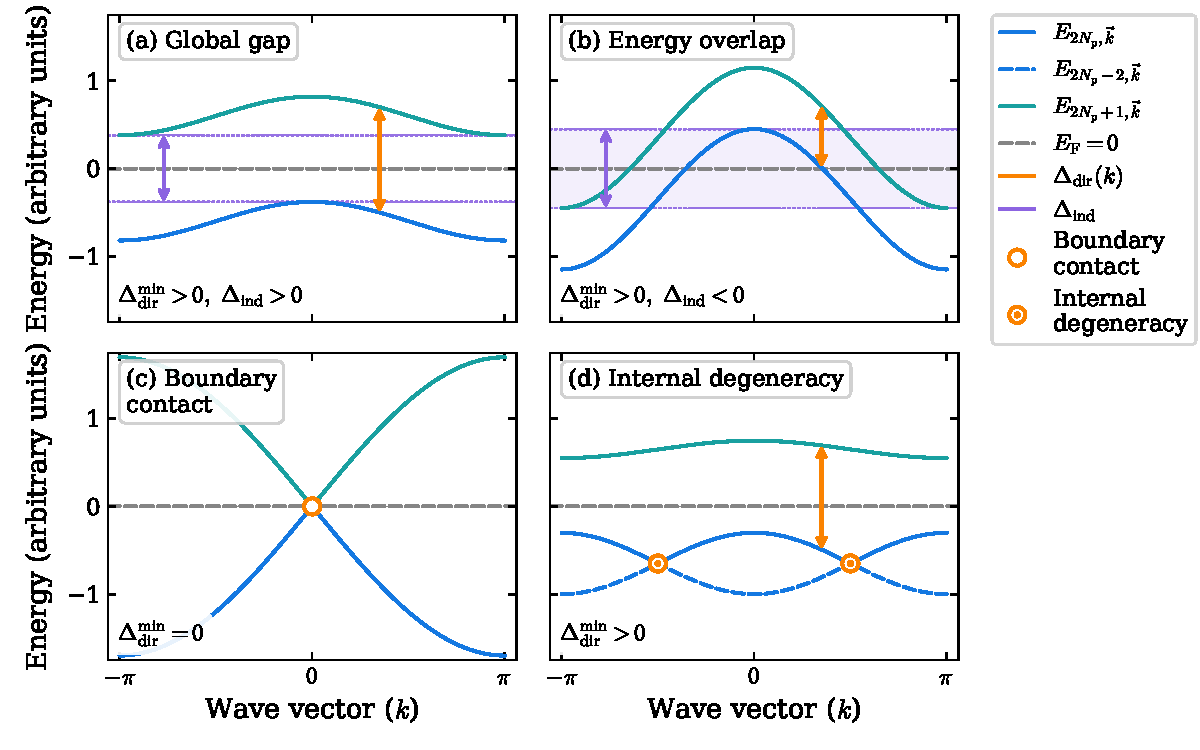
\includegraphics[width=0.8\textwidth]{figures_ch4/4.1_band_subspace.pdf}
\caption{Schematic distinction between an isolated band subspace and an insulating gap.
(a) Global gap, (b) indirect energy overlap, (c) contact between selected and excluded bands,
and (d) degeneracy within the selected subspace.}
\label{fig:band_subspace_and_insulating_gap}
\end{figure}

In figure~\ref{fig:band_subspace_and_insulating_gap}(a), positive direct and indirect gaps permit an insulating filling.
In (b), the direct gap remains positive despite the indirect energy overlap.
Both situations permit a smooth fixed-rank projector, provided the direct gap remains positive over the full two-dimensional Brillouin zone.
In (c), a band touching closes the direct gap between the selected and excluded bands.
In (d), both pairs belong to the selected subspace on either side of the degeneracy.
The plotted energies remain ordered, so $E_{2N_\mathrm{p}-2,\vec{k}}\leq E_{2N_\mathrm{p},\vec{k}}$ throughout the cut.
Following this energy order through a crossing can give a cusp in the plotted eigenvalues,
although the hamiltonian and the projector onto both pairs remain smooth.
Since the direct gap remains positive, this internal degeneracy does not prevent the selected subspace from varying smoothly.
We now examine the symmetries that constrain these states,
while keeping the separate question of the physical Fermi level explicit.

\newpage
\section{Time-reversal and inversion symmetry}
\label{sec:symmetry_and_kramers_pairs_topology}

% opening paragraph
The previous section identified the isolated band subspace.
The geometric construction in appendix~\ref{cha:appendix_topology} explains why its global character involves how the states are connected across the Brillouin zone.
We now impose the symmetries relevant to the beryllene parity analysis.
Time reversal connects states at opposite wave vectors and determines their Kramers pairing.
Inversion also reverses the wave vector, while assigning a parity at the points where the state returns to an equivalent wave vector.
Together, these two symmetries provide the information used in the parity criterion.

\subsection{Kramers pairing in the spinful calculation}

Equation~\eqref{KS_spinor_equation_method} supplies the spinor states used in the calculation.
The two spin components belong to one electronic state.
Spin-orbit coupling can mix these components without breaking time-reversal symmetry.
We therefore retain the full spinor when identifying the time-reversed partner.

For spin-$1/2$ electrons, the time-reversal operator satisfies $\hat{\Theta}^2=-\hat{I}$.
When the hamiltonian preserves this symmetry,
$\hat{\Theta}\hat{h}(\vec{k}\,)\hat{\Theta}^{-1}=\hat{h}(-\vec{k}\,)$.
The operator convention and the derivation of Kramers pairing are given in section~\ref{sec:spinors_time_reversal_appendix} of appendix~\ref{cha:appendix_topology}.
At a general wave vector, time reversal relates a state at $\vec{k}$ to an equal-energy state at $-\vec{k}$.
At a wave vector equivalent to its negative, these are two orthogonal states at the same wave vector and form a Kramers pair.
The parity calculation must count these complete pairs.
We now identify the momenta at which this pairing and inversion parity can be used together.

\subsection{Time-reversal invariant momenta}
\label{subsec:trim_topology}

We now identify the wave vectors at which Kramers pairing occurs at the same point of the Brillouin zone.
The wave vector is defined modulo a reciprocal-lattice vector.
A time-reversal invariant momentum, abbreviated as TRIM, therefore satisfies:

\begin{equation}
    \vec{\Lambda}_i=-\vec{\Lambda}_i+\vec{G}_i
\label{trim_condition_topology}
\end{equation}

here, $\vec{G}_i$ is a reciprocal-lattice vector.
For a two-dimensional reciprocal basis $\vec{b}_1$ and $\vec{b}_2$,
the four inequivalent solutions can be represented as:

\begin{equation}
    \vec{\Lambda}_{n_1n_2}
    =\frac{n_1\vec{b}_1+n_2\vec{b}_2}{2},
    \qquad n_1,n_2\in\{0,1\}
\label{four_trim_two_dimensions_topology}
\end{equation}

We count these points by rewriting equation~\eqref{trim_condition_topology} as $2\vec{\Lambda}_i=\vec{G}_i$.
The two coefficients of $\vec{G}_i$ in the reciprocal basis are integers.
Increasing either integer by two changes $\vec{\Lambda}_i$ by a full reciprocal-lattice vector,
so it gives an equivalent wave vector.
Only the even or odd choice of each coefficient matters, leaving $2\times2=4$ inequivalent points.

Their names depend on the reciprocal lattice.
For the hexagonal Brillouin zone of a triangular lattice,
they are $\Gamma$ and three inequivalent $\mathrm{M}$ points.
For a square lattice, they are $\Gamma$, two edge-centre points, and the corner point $\mathrm{M}$.
We label the two edge-centre representatives as $\mathrm{X}$ and $\mathrm{Y}$
to keep all four points explicit before using any additional rotational symmetry.
Figure~\ref{fig:four_trim_two_dimensions} shows these two Brillouin zones.
The representatives follow equation~\eqref{four_trim_two_dimensions_topology},
with reciprocal-lattice translations used where necessary to place them in the displayed zones.
The diagrams indicate wave-vector locations only.
Each colour identifies one inequivalent TRIM and its periodic copies within a panel.

\begin{figure}[htbp]
\centering
    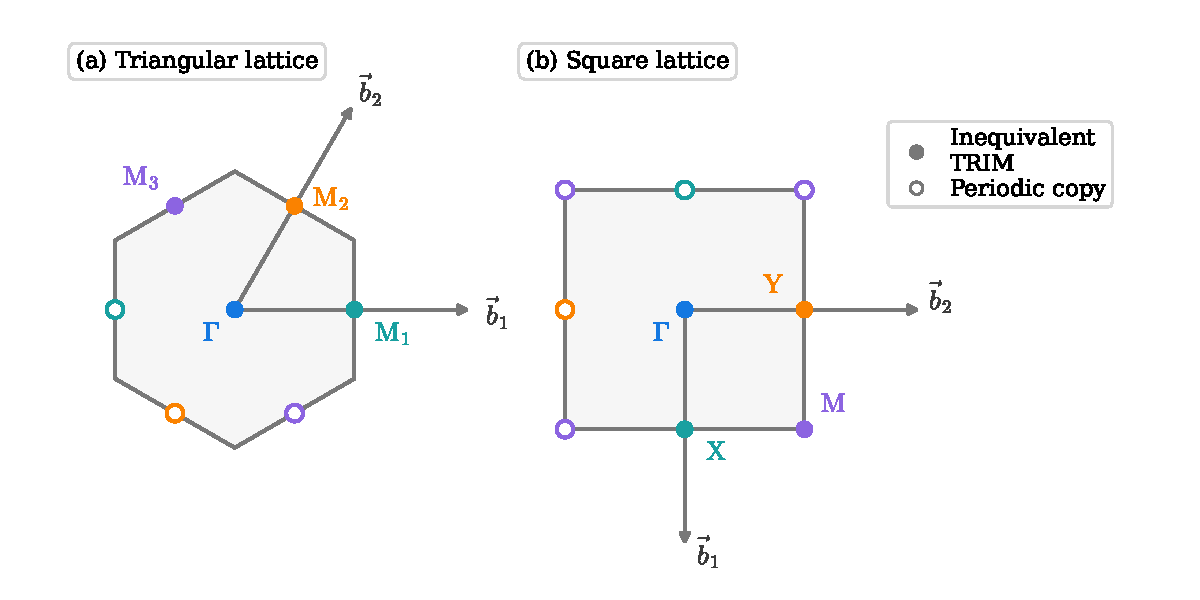
\includegraphics[width=0.8\textwidth]{figures_ch4/4.2_trim.pdf}
\caption{Time-reversal invariant momenta in schematic Brillouin zones of (a) triangular and (b) square lattices.
Filled points identify inequivalent TRIM; open points mark periodic boundary copies.}
\label{fig:four_trim_two_dimensions}
\end{figure}

The boundary copies in figure~\ref{fig:four_trim_two_dimensions} do not provide additional independent factors in the parity product.
They represent equivalent wave vectors related by a reciprocal-lattice translation.
Likewise, the corners conventionally denoted by $\mathrm{K}$ in the hexagonal Brillouin zone are not TRIM.
Time reversal exchanges the two inequivalent corners rather than returning either one to itself.

\subsection{Inversion and the parity of a Kramers pair}

We next introduce the inversion operator $\hat{\mathcal{I}}$.
We choose the real-space origin at an inversion centre,
so inversion changes $\vec{r}$ to $-\vec{r}$ and leaves spin unchanged.
Its action on a Bloch state can be expressed through a position projection:

\begin{equation}
    \bra{\vec{r}\,}\hat{\mathcal{I}}\ket{\psi_{n\vec{k}}}
    =\braket{-\vec{r}\,|\psi_{n\vec{k}}}
\label{inversion_position_projection_topology}
\end{equation}

here, the projection leaves the spin components implicit.
For an inversion-symmetric hamiltonian, we have:

\begin{equation}
\left\{\begin{aligned}
    \hat{\mathcal{I}}^2&=\hat{I} \\
    \hat{\mathcal{I}}\hat{h}(\vec{k}\,)\hat{\mathcal{I}}^{-1}
    &=\hat{h}(-\vec{k}\,) \\
    [\hat{\mathcal{I}},\hat{\Theta}]&=0
\end{aligned}\right.
\label{inversion_symmetry_relations_topology}
\end{equation}

Both inversion and time reversal reverse the wave vector.
Their combination consequently leaves $\vec{k}$ unchanged.
Since $(\hat{\mathcal{I}}\hat{\Theta})^2=-\hat{I}$,
the antiunitary argument in section~\ref{sec:spinors_time_reversal_appendix} of appendix~\ref{cha:appendix_topology}
gives a twofold degeneracy at every $\vec{k}$
when both symmetries are present.
At the TRIM, we can additionally choose the states to diagonalize inversion.

At a TRIM, inversion maps a Bloch state to an equivalent wave vector modulo a reciprocal-lattice vector.
We can therefore choose the full Bloch states with definite inversion parity and write:

\begin{equation}
    \hat{\mathcal{I}}\ket{\psi_{n\vec{\Lambda}_i}}
    =\xi_n(\vec{\Lambda}_i\,)\ket{\psi_{n\vec{\Lambda}_i}},
    \qquad \xi_n(\vec{\Lambda}_i\,)=\pm1
\label{parity_eigenvalue_topology}
\end{equation}

here, $\xi_n$ is the parity eigenvalue.
Applying inversion twice gives $\xi_n^2\ket{\psi_{n\vec{\Lambda}_i}}=\ket{\psi_{n\vec{\Lambda}_i}}$,
so the eigenvalue can only be $+1$ or $-1$.
The values $+1$ and $-1$ describe even and odd inversion parity, respectively.
An even state is unchanged under inversion, while an odd state changes sign.
This sign describes the transformation of the state.
The probability density is unchanged in both cases.
Within a degenerate eigenspace, the states can be chosen as simultaneous energy and parity eigenstates.
An arbitrary numerical basis of that eigenspace can mix these eigenstates.

We can also express the same parity relation using the cell-periodic states.
Inversion changes the sign in the Bloch factor of equation~\eqref{bloch_hamiltonian_topology}.
Substituting this factor into equation~\eqref{parity_eigenvalue_topology}, with $\vec{G}_i=2\vec{\Lambda}_i$, gives:

\begin{equation}
\left\{\begin{aligned}
    \hat{\mathcal{I}}\ket{u_{n\vec{\Lambda}_i}}
    &=\xi_n(\vec{\Lambda}_i\,)
    \mathrm{e}^{\mathrm{i}\vec{G}_i\cdot\hat{\vec{r}}}\ket{u_{n\vec{\Lambda}_i}} \\
    \mathrm{e}^{-\mathrm{i}\vec{G}_i\cdot\hat{\vec{r}}}
    \hat{\mathcal{I}}\ket{u_{n\vec{\Lambda}_i}}
    &=\xi_n(\vec{\Lambda}_i\,)\ket{u_{n\vec{\Lambda}_i}}
\end{aligned}\right.
\label{cell_periodic_parity_topology}
\end{equation}

here, the reciprocal-lattice factor returns the inverted state to the chosen representative of the TRIM.
At $\Gamma$, this factor is unity.
At a non-zero TRIM, it enters the full Bloch-state parity extracted from a cell-periodic representation.
Thus the two representations give the same $\xi_n$ when their boundary identification is treated consistently.

We now apply inversion to the time-reversed partner.
Since inversion commutes with time reversal and $\xi_n$ is real, we obtain:

\begin{equation}
\begin{aligned}
    \hat{\mathcal{I}}\hat{\Theta}\ket{\psi_{n\vec{\Lambda}_i}}
    &=\hat{\Theta}\hat{\mathcal{I}}\ket{\psi_{n\vec{\Lambda}_i}} \\
    &=\xi_n(\vec{\Lambda}_i\,)
    \hat{\Theta}\ket{\psi_{n\vec{\Lambda}_i}}
\end{aligned}
\label{equal_parity_kramers_pair_topology}
\end{equation}

Therefore, the two states of a Kramers pair have the same parity.
This result determines how parity eigenvalues are counted in the topological criterion.
Counting both states separately would square every pair contribution and remove the sign information that we need.

\newpage
\section{From parity eigenvalues to the two-dimensional \texorpdfstring{$\mathbb{Z}_2$}{Z2} index}
\label{sec:fu_kane_criterion_topology}

% opening paragraph
We have now established the selected band subspace, its phase freedom, and the pairing imposed by symmetry.
The remaining question is whether this subspace can change its topological character continuously while preserving time-reversal symmetry and its separation from the excluded bands.
The two-dimensional $\mathbb{Z}_2$ index distinguishes two possibilities for this spinful band problem~\cite{kane2005z2}.
Inversion symmetry then allows us to evaluate that index using the parity information at the four TRIM~\cite{wieder2022topological}.
Time reversal is the symmetry that protects this $\mathbb{Z}_2$ classification;
inversion supplies the simpler route for evaluating it.
If inversion is removed along a continuous change that preserves time reversal and the band separation,
the index remains unchanged, although the parity criterion is no longer available.

\subsection{The two topological classes}

We first consider a continuous change of the hamiltonian,
such as a change in bond geometry or in the strength of spin-orbit coupling.
As long as the selected subspace remains isolated and time-reversal symmetry is preserved,
its $\mathbb{Z}_2$ index cannot change.
We denote the two possible values by $\nu=0$ and $\nu=1$.
The former is trivial with respect to this index, while the latter is non-trivial.

In terms of electronic states, we use the basis freedom developed in equation~\eqref{band_subspace_basis_transformation_topology} of appendix~\ref{cha:appendix_topology}.
The distinction concerns whether a globally smooth basis can be chosen
with a consistent time-reversal pairing and the reciprocal-lattice identification introduced above.
Here, a local choice covers only a neighbourhood of one wave vector.
A global choice must join these local choices over the whole Brillouin zone, including its identified boundaries,
while preserving the relation between each state and its time-reversed partner.
For $\nu=1$, this time-reversal-compatible choice is obstructed~\cite{fu2006time}.
The projector itself remains continuous, and smooth choices of basis still exist.
The constraint comes from requiring the basis to satisfy the time-reversal pairing as well as the global continuity conditions~\cite{kane2005z2}.

For an insulating filling, this distinction has a physical consequence at an interface with a topologically trivial insulator.
Within the non-interacting description and with time-reversal symmetry preserved at the boundary,
the non-trivial phase supports an odd number of Kramers pairs of edge modes connecting the bulk bands~\cite{kane2005z2}.
These edge states are helical.
Time-reversed partners propagate in opposite directions and have opposite spin expectation values.
This relation holds even when spin-orbit coupling mixes the spin components.

For a single pair, we consider a static one-electron perturbation $\hat{V}$ that is Hermitian and preserves time reversal.
The antiunitary relation used in equation~\eqref{kramers_orthogonality_topology} of appendix~\ref{cha:appendix_topology} gives:

\begin{equation}
    \bra{\hat{\Theta}\psi}\hat{V}\ket{\psi}=0,
    \qquad
    \hat{V}^{\dagger}=\hat{V},\quad
    [\hat{V},\hat{\Theta}]=0
\label{helical_edge_backscattering_topology}
\end{equation}

here, $\ket{\psi}$ and $\hat{\Theta}\ket{\psi}$ are the two time-reversed edge states.
Thus this perturbation cannot produce elastic backscattering between the partners~\cite{kane2005z2}.
The statement concerns a single edge within the one-electron description.
Bulk conduction and inelastic processes can still dissipate the current.
For a metallic filling, bulk states can remain at the Fermi level,
so the insulating-edge interpretation requires more than the parity sign.

\subsection{The Fu--Kane parity product}

We now use inversion symmetry to evaluate $\nu$.
For each TRIM $\vec{\Lambda}_i$, we first multiply one parity eigenvalue from each of the $N_\mathrm{p}$ Kramers pairs in the selected subspace:

\begin{equation}
    \delta_i
    \coloneqq\prod_{m=1}^{N_\mathrm{p}}\xi_{2m}(\vec{\Lambda}_i\,)
\label{parity_product_at_trim_topology}
\end{equation}

here, the indices $(2m-1,2m)$ label two states related by time reversal within the $m$th Kramers pair.
Their equal parity follows from equation~\eqref{equal_parity_kramers_pair_topology}.
If several pairs share the same energy, we resolve inversion within that eigenspace and pair its states by time reversal,
as the energy ordering leaves these partners open.
The subspace contains $2N_\mathrm{p}$ spinor states, but the product contains $N_\mathrm{p}$ factors.
The use of $2m$ selects one representative from each pair.

The Fu--Kane criterion relates these four products to the two-dimensional index~\cite{fu2007topological}:

\begin{equation}
\left\{\begin{aligned}
    (-1)^\nu&=\prod_{i=1}^{4}\delta_i \\
    \nu&=
    \begin{cases}
        0, & \prod_{i=1}^{4}\delta_i=+1 \\
        1, & \prod_{i=1}^{4}\delta_i=-1
    \end{cases}
\end{aligned}\right.
\label{fu_kane_index_topology}
\end{equation}

We can read these products in two steps.
At one TRIM, an odd number of odd-parity Kramers pairs gives $\delta_i=-1$,
whereas an even number gives $\delta_i=+1$.
We then count how many of the four TRIM have a negative product.
For example, if $(\delta_1,\delta_2,\delta_3,\delta_4)=(-1,+1,+1,+1)$,
the total product is $-1$ and $\nu=1$.
If a second product changes from $+1$ to $-1$, the total becomes $+1$ and $\nu=0$.
These illustrative signs show that the index records an even or odd count.

The equality of the two parities in each pair explains the counting in equation~\eqref{parity_product_at_trim_topology}.
Identifying the four-point product with $(-1)^\nu$ is an additional topological result.
Fu and Kane derive this identification from the symmetry transformation of the Bloch basis~\cite[sections II and III]{fu2007topological}.
The criterion evaluates the global time-reversal obstruction,
which is distinct from a single-band Berry phase on an arbitrary loop.

The result also explains why the parity of a single state or the ordering at one wave vector is insufficient.
Every selected Kramers pair contributes at each of the four TRIM.
If one selected pair exchanges with an excluded pair of opposite parity at a TRIM,
that exchange changes the local product when the gap reopens.
An odd number of such sign changes alters the global product,
whereas an even number leaves it unchanged.
If inversion is preserved throughout the exchange, the separation between the two subspaces must close at that TRIM.
An exchange wholly within the selected subspace instead preserves the product because neither pair leaves the count.

\subsection{Using additional crystal symmetry}

For the hexagonal Brillouin zone in figure~\ref{fig:four_trim_two_dimensions}(a),
the general product is:

\begin{equation}
    (-1)^\nu
    =\delta_\Gamma\delta_{\mathrm{M}_1}
    \delta_{\mathrm{M}_2}\delta_{\mathrm{M}_3}
\label{hexagonal_trim_product_topology}
\end{equation}

If crystal symmetry relates the three $\mathrm{M}$ points with equal parity products in the chosen inversion convention,
we can stipulate $\delta_{\mathrm{M}_1}=\delta_{\mathrm{M}_2}=\delta_{\mathrm{M}_3}=\delta_\mathrm{M}$.
The product then reduces to $\delta_\Gamma(\delta_\mathrm{M})^3=\delta_\Gamma\delta_\mathrm{M}$.

For the square Brillouin zone in figure~\ref{fig:four_trim_two_dimensions}(b),
we similarly retain all four representatives first:

\begin{equation}
    (-1)^\nu
    =\delta_\Gamma\delta_\mathrm{X}\delta_\mathrm{Y}\delta_\mathrm{M}
\label{square_trim_product_topology}
\end{equation}

If the actual structure relates $\mathrm{X}$ and $\mathrm{Y}$ with equal parity products,
then $\delta_\mathrm{X}\delta_\mathrm{Y}=(\delta_\mathrm{X})^2=1$,
and the same reduced expression follows.
A fourfold rotation about the chosen inversion centre can give this equality;
the two symmetry-equivalent representatives may then both be called $\mathrm{X}$ points.
The equality of the final expressions results from different symmetry relations among their four TRIM,
and the two Brillouin zones remain inequivalent.

We therefore retain all four factors in equation~\eqref{fu_kane_index_topology} until the symmetry of the calculated structure
and the inversion convention establish these equalities.
The reduction follows from these symmetries, whatever high-symmetry path is plotted.

\newpage
\section{From the parity criterion to the calculation}
\label{sec:interpreting_topology_calculation}

% opening paragraph
The previous section connected the parity eigenvalues to the $\mathbb{Z}_2$ index.
We now return to the first-principles setting introduced in subsection~\ref{subsec:method_topology}.
The calculation must supply the same ingredients used in that connection, namely a specified spinor hamiltonian, the relevant symmetries, an isolated band subspace, and the parity of its Kramers pairs.
The interpretation then follows from the relation between that subspace and the Fermi level.

\subsection{Identifying the states used in the product}

We first determine the crystal symmetry and the reciprocal lattice of the relaxed structure.
These determine the inversion operation and the four TRIM.
For the spinful classification used here, the electronic states are calculated with spin-orbit coupling,
and the reference state must preserve time-reversal symmetry.
We retain spin-orbit coupling even for a light element~\cite{molle2017buckled},
since a small coupling may still affect a band crossing or a small separation relevant to the selected subspace.

We then select the fixed number $2N_\mathrm{p}$ of bands and examine
$\Delta_\mathrm{dir}(\vec{k}\,)$ from equation~\eqref{minimum_direct_gap_topology}.
For an insulator whose occupied bands form this subspace, $2N_\mathrm{p}=N_\mathrm{occ}$,
where $N_\mathrm{occ}$ counts occupied spinor bands rather than Kramers pairs.
In this insulating case, equations~\eqref{parity_product_at_trim_topology} and~\eqref{fu_kane_index_topology}
have the occupied-band counting used in equations~\eqref{eq:proj3_parity_product} and~\eqref{eq:proj3_z2_index} of chapter~\ref{cha:project_beryllene}.
For a metal, the number of states below $E_\mathrm{F}$ can change with $\vec{k}$,
so the phrase ``occupied bands'' leaves the subspace ambiguous.
Numerical smearing of the occupations also does not define a fixed-rank projector.
The band count instead refers to the selected spectral subspace at every wave vector.

The direct gap has to be checked over the two-dimensional Brillouin zone.
Its positivity at the four TRIM or along a plotted high-symmetry path covers only part of that zone.
In practice, a converged two-dimensional sampling, with refinement near the smallest direct gaps,
provides evidence for the gap condition within the numerical accuracy of the calculation.
If interpolation is used, direct calculations near those gaps verify its accuracy.
A near-zero direct gap is refined further, because an unresolved touching point changes whether the chosen spectral subspace is isolated.

At each TRIM, the parity eigenvalues can be obtained from the symmetry representation of the spinor states.
The \texttt{IrRep} code used in chapter~\ref{cha:project_beryllene}
extracts such symmetry information from \texttt{VASP} wave functions~\cite{iraola2022irrep}.
Equation~\eqref{cell_periodic_parity_topology} explains the reciprocal-lattice identification required by a cell-periodic representation.
For a degenerate group, we resolve the inversion representation within that group,
which separates the parity eigenstates from an arbitrary numerical mixture.
We then identify complete Kramers pairs, count one parity from each pair,
and evaluate the four factors in equation~\eqref{parity_product_at_trim_topology}.

\subsection{Interpreting the resulting index}

Once the isolation and symmetries of the selected spectral subspace have been established, the parity criterion classifies this subspace.
We then compare its energy range with the physical Fermi level.
If equation~\eqref{insulating_fermi_level_topology} holds,
the subspace is the occupied space of a band insulator,
and $\nu=1$ identifies the non-trivial two-dimensional time-reversal phase within the band description.

If the direct gap remains positive but the indirect gap is negative,
we can still discuss the topology of the isolated lower-band subspace.
The actual Fermi-level state nevertheless remains metallic at an overlapping filling.
Thus the topological index and the metallic character describe different aspects of the same band structure,
as illustrated in figure~\ref{fig:band_subspace_and_insulating_gap}(b).
If the selected and excluded bands touch,
the isolation condition used throughout this chapter is absent,
and applying this fixed-rank spectral-subspace argument requires further justification.

This distinction also clarifies the relation to the optical analysis.
The independent-particle response in equation~\eqref{independent_particle_imaginary_dielectric_tensor}
uses actual occupation differences, transition matrix elements, and transition energies.
The parity criterion instead characterizes the connection of a specified band subspace over the Brillouin zone.
The optical spectrum therefore resolves the allowed electronic excitations,
while the parity product classifies the symmetry-constrained connection of the selected states.
The Fermi-level condition determines whether this classification describes an insulating phase.

Chapters~\ref{cha:fundamentals_a} and~\ref{cha:fundamentals_b} supply the electronic structure and its linear optical response, respectively.
The present chapter establishes the band-subspace and symmetry conditions for topology.
The material-specific band selection, gap evidence, and parity eigenvalues determine which interpretation applies to each system.

\cleardoublepage
\chapter[Optoelectronics of Carbon-Boron Heterostructures]{Electronic and Optical Properties of 2D Heterostructure Bilayers of Graphene, Borophene and 2D Boron Carbides from First Principles}
\label{cha:project_bilayers}

This chapter is based on the article by L.~Niu, O.~J.~Conquest, C.~Verdi, and C.~Stampfl,
published in \textit{Nanomaterials} \textbf{14}, 1659 (2024)~\cite{niu2024electronic}.
The candidate performed the investigation, formal analysis, software development, data curation, and visualization.
Catherine Stampfl conceived the study and provided the computational resources.
All four authors contributed to the methodology and the original manuscript;
the candidate, Oliver James Conquest, and Carla Verdi performed the validation.
Catherine Stampfl, Carla Verdi, and Oliver James Conquest supervised and administered the project, and reviewed and edited the manuscript.

\section{Abstract}
\label{1_abstract}

In this chapter,
we investigate the atomic, electronic, and optical properties of two-dimensional heterostructure bilayers,
namely Graphene-\ce{BC3}, Graphene-Borophene, and Graphene-\ce{B4C3},
as well as their constituent monolayers, on the basis of first-principles calculations using the HSE06 hybrid functional.
The calculations show that while borophene is metallic,
both monolayer \ce{BC3} and \ce{B4C3} are indirect semiconductors,
with band gaps of \qty{1.822}{\electronvolt} and \qty{2.381}{\electronvolt} as obtained using HSE06.
The Graphene-\ce{BC3} and Graphene-\ce{B4C3} bilayer heterojunction systems maintain the Dirac point of graphene at the $\mathrm{K}$ point and are semimetals,
while Graphene-Borophene is metallic.
All bilayer heterostructure systems exhibit absorption in the visible region, where the resonance frequency and resonance absorption peak intensity vary between structures.
In addition, all heterojunctions show spectral features consistent with plasmon resonances at approximately \qtyrange{17}{19}{\electronvolt}, while Graphene-\ce{B4C3} and Graphene-Borophene show low-energy features in the in-plane dielectric response within the region \qtyrange{4}{6}{\electronvolt},
with the latter possessing an additional feature at the lower energy of \qtyrange{1.5}{3}{\electronvolt}.
The dielectric response differs strongly between in-plane and out-of-plane polarizations.
The heterostructures show visible-light absorption and plasmon-related features that shift with the boron-based monolayer, indicating tunable optoelectronic behaviour.

\clearpage
\section{Introduction}
\label{1_introduction}

Graphene has excellent electrical conductivity,
desirable mechanical and thermal properties,
and high light transmittance in the visible-light and infrared regions.
It also has an extremely high quantum efficiency for light-matter interactions and is strongly optically non-linear.
These properties have therefore enabled applications in e.g. electronics, energy storage, biomedical devices, and other fields~\cite{janavika2023graphene}.
Relative to conventional plasmonic materials, graphene possesses highly confined plasmons with much longer lifetimes.
In addition, graphene plasmons are active in an extended wavelength range, namely, the mid-infrared and terahertz regime.
This wavelength range overlaps with the characteristic signals of most organic and biomolecules,
which has broadened graphene's applications towards plasmonic biological and chemical sensors~\cite{sakthivel2023} in addition to plasmonic waveguides
and infrared photodetectors.
Moreover, forming graphene-hybrid materials can tune the properties of graphene, finding applications in biosensors, chemical sensors, optical sensors, and other types of sensors~\cite{zhang2022}.

In other areas, however, the use of graphene remains limited by its zero band gap.
One method used to expand the application of graphene is to form heterostructures.
Stacking different two-dimensional (2D) materials together can form double-layer or even multi-layer artificial materials that are maintained by van der Waals interactions~\cite{novoselov20162d}.
Such materials are known as van der Waals heterojunctions.
Such stacking can generate a wide range of physical properties,
making van der Waals heterojunctions even more important than the individual 2D materials themselves.
There are vast numbers of 2D materials, and by forming heterostructures thereof,
a diverse range of electrical, photonic, plasmonic, mechanical, and chemical properties can be theoretically predicted through \textit{ab initio} calculations and machine learning~\cite{thygesen2017,he2023}, and experimentally engineered~\cite{lin2023recent,elbanna20232d}.

Recently, the prospect of developing plasmonic devices employing 2D semiconductors has attracted considerable attention~\cite{agarwal2018plasmonics, qiu2018optical}.
Plasmonic modes in each class of van der Waals semiconductors have their own peculiarities, along with potential technological capabilities.
Graphene-like \ce{BC3} has also been synthesized experimentally~\cite{yanagisawa2004phonon, yanagisawa2006phonon, tanaka2005novel} and is found to be semiconducting with an indirect band gap.
Calculations have shown that nanostructures of graphene-like \ce{BC3} exhibit desirable absorption in the visible region and, by changing the size of the nanostructure,
the resonance peak position of the absorption spectrum can be effectively regulated~\cite{chen2019plasmon}.
Recent studies have also predicted a stable \ce{B4C3} monolayer,
which is even more stable than the previously synthesized \ce{BC3} monolayer~\cite{tian2019}.
Boron carbides are known for their exceptional hardness,
thermal stability, and chemical inertness.
The emergence of 2D boron carbides adds a new dimension to the study of these materials,
offering novel properties and opportunities for technological innovation~\cite{luo2011predicting,fan2018two}.

Borophene is another 2D material of high current interest.
This monolayer allotrope of boron forms several structures and is characterized by its unique atomic structure and exceptional electronic properties,
which have opened new avenues for innovation in the areas of electronics,
energy storage, catalysis, plasmonics, superconductivity, and sensors~\cite{qiu2018optical}.
One particularly intriguing aspect of borophene's versatility lies in its ability to form heterojunctions---interfaces between different borophene structures or between borophene and other materials.
Borophene-graphene heterostructures have been realized~\cite{hou2021borophene},
where they have shown good stability and the ability to function as humidity sensors,
exhibiting a sensitivity about 700 times higher than that of pristine graphene,
and 27 times higher than that of borophene.
Recently, both lateral and vertical integration of borophene with graphene has also been achieved~\cite{liu2019borophene},
as has the formation of bilayer ($\alpha$-phase) borophene on the Ag(111) surface~\cite{liu2022}.

Graphene contributes conductivity and flexibility; boron carbide adds structural and chemical stability; borophene provides electronic tunability.
These features make the resulting heterostructures relevant to electronic, optoelectronic, energy-storage, and sensing devices.
As research in this field continues to advance,
the development of scalable synthesis methods, the elucidation of structure-property relationships,
and the exploration of novel applications will be key focal points.
To date, little is known about the physical properties of graphene-based bilayer heterojunctions with borophene and boron-carbide materials.
This motivates the present chapter to gain an understanding of these heterojunctions
through the study of their electronic and optical properties on the basis of first-principles calculations.
The comparison with the constituent monolayers identifies how stacking changes the band alignment, charge redistribution, and polarization-dependent optical response.
These structure-property relationships provide the main contribution of this chapter,
while the performance of a fabricated device lies outside its scope.

This chapter is organized as follows:
In section~\ref{1_calculation_methods}, the calculation method is described,
followed by the Results and Discussion in section~\ref{1_results}.
Herein, we describe the physical properties of the monolayers and heterostructures, including band structure, density of states, electron-density difference distributions,
Schottky barriers and the optical properties.
This is followed by the Conclusion in section~\ref{1_conclusions}.

\section{Calculation methods}
\label{1_calculation_methods}

We perform first-principles calculations using density functional theory (DFT) as implemented in the Vienna Ab initio Simulation Package (\texttt{VASP})~\cite{kresse1993ab, kresse1996efficiency, kresse1996efficient}.
Projector augmented wave (PAW) pseudopotentials account for the electron-ion interactions~\cite{kresse1999ultrasoft}.
For the structural optimization calculations, we use the generalized gradient approximation (GGA) of Perdew--Burke--Ernzerhof (PBE) as the exchange-correlation functional.
The Becke--Johnson damped D3(BJ) dispersion correction accounts for long-range van der Waals (vdW) interactions.
The structural calculations use a $\Gamma$-centred k-point sampling mesh of $11 \times 11 \times 1$, except for the smaller graphene unit cell shown in figure~\ref{fig1.1}, for which a denser mesh of $23 \times 23 \times 1$ is used.
Figure~\ref{S1.1} shows the k-point convergence test for the Graphene-\ce{BC3} bilayer.
Here, the plane-wave energy cutoff is set to \qty{450}{\electronvolt}.
The electronic convergence criterion is set to \qty{1e-6}{\electronvolt}, and the systems are allowed to relax until all forces on each atom are below \qty{0.01}{\electronvolt\per\angstrom}.
For smearing at the Fermi level,
we use the Gaussian smearing method implemented in \texttt{VASP}.

For the calculation of electronic properties,
the PBE exchange-correlation functional is known to underestimate band-gap energies.
Therefore, we also use the screened hybrid exchange-correlation functional of Heyd, Scuseria, and Ernzerhof (HSE06),
which can improve the description of band-gap energies relative to PBE~\cite{sassnick2021electronic, heyd2003hybrid, krukau2006influence}.

For the total density of states (DoS) shown with the band structures,
we use a $\Gamma$-centred k-point sampling mesh of $33 \times 33 \times 1$.
The atom- and orbital-projected HSE06 densities of states use the $17 \times 17 \times 1$ mesh,
with the total and projected contributions referred to the same Fermi energy for each calculation.
Both use Gaussian smearing with a broadening value of \qty{0.1}{\electronvolt}.
The HSE06 exchange-correlation functional is also used for the calculation of optical properties,
in particular, the frequency-dependent dielectric function with $\Gamma$-centred k-point sampling meshes of $17 \times 17 \times 1$ and $65 \times 65 \times 1$.
The complex frequency-dependent dielectric function, $\varepsilon(\omega)$,
is given by equation~\eqref{complex_dielectric_function_definition};
here, $\varepsilon_{1}(\omega)$ and $\varepsilon_{2}(\omega)$ are the real and imaginary parts, respectively, and $\omega$ denotes the angular frequency.
The spectra are plotted against the photon energy $\hbar\omega$ in \unit{\electronvolt}.

We then use the dielectric function to calculate the absorption coefficient,
refractive index, extinction coefficient, reflectivity, and energy-loss spectrum,
following the relations introduced in section~\ref{sec:from_dielectric_function_to_optical_properties}.
These scalar relations apply to the diagonal response along a principal direction.
The diagonal spectra are used below in the principal-axis description.

The interlayer binding energy $E_{\mathrm{b}}$ follows as:

\begin{equation}
E_{\mathrm{b}}
= E_{\mathrm{H}} - E_{\mathrm{BC}/\mathrm{B}} - E_{\mathrm{G}}
\label{interlayer_binding_energy}
\end{equation}

here, $E_{\mathrm{H}}$ denotes the total energy of the heterostructure,
$E_{\mathrm{BC}/\mathrm{B}}$ corresponds to the total energy of the isolated boron-carbide or borophene monolayer,
and $E_{\mathrm{G}}$ denotes the total energy of the isolated graphene monolayer.

Afterwards, the charge-density difference $\Delta \rho(\vec{r}\,)$ takes the form:

\begin{equation}
\Delta \rho(\vec{r}\,) =
\rho_{\mathrm{AB}}(\vec{r}\,)
- \rho_{\mathrm{A}}(\vec{r}\,)
- \rho_{\mathrm{B}}(\vec{r}\,)
\label{charge_density_difference}
\end{equation}

here, $\rho_{\mathrm{AB}}(\vec{r}\,)$ denotes the total charge density of the heterostructure.
The terms $\rho_{\mathrm{A}}(\vec{r}\,)$ and $\rho_{\mathrm{B}}(\vec{r}\,)$ represent the charge densities of the isolated monolayers forming the heterostructure.

\section{Results and discussion}
\label{1_results}

\subsection{Monolayer properties}

We first examine the structural and electronic properties of the three non-graphene monolayers,
namely \ce{BC3}, \ce{B4C3}, and borophene.
Graphene is also investigated because it always forms one layer of the heterostructure systems.
The optimized structures of \ce{BC3}, \ce{B4C3}, borophene,
and graphene are shown in figure~\ref{fig1.1}.
Borophene monolayers have been predicted to possess various low-energy structures,
among which the $\beta_{12}$, $\chi_{3}$, and $\alpha'$ structures have been synthesized experimentally~\cite{kaneti2021borophene}.
For this study, we choose to investigate the $\alpha'$ structure of borophene,
not only because it has been synthesized experimentally,
but also because GGA-level \textit{ab initio} calculations have shown it to have the most favourable cohesive energy~\cite{wu2012two}.

The structural properties and band-gap energies of the monolayer systems are shown in table~\ref{tab:1.1_monolayer}.
For graphene, the calculated lattice constant is $a = \qty{2.467}{\angstrom}$,
while those of borophene, \ce{BC3}, and \ce{B4C3} are \qty{5.051}{\angstrom}, \qty{5.169}{\angstrom}, and \qty{4.690}{\angstrom}, respectively.
In agreement with previous calculations, graphene is a semimetal and borophene is metallic,
whereas \ce{BC3} and \ce{B4C3} are indirect semiconductors~\cite{zhang2018strain, nosheen2022first}.
The calculated indirect band gaps of \ce{BC3} and \ce{B4C3} are \qty{1.822}{\electronvolt} (\qty{0.634}{\electronvolt}) and \qty{2.381}{\electronvolt} (\qty{1.647}{\electronvolt}), respectively, as obtained using HSE06 (PBE).

Figure~\ref{S1.2} shows the optimization of the lattice constants for the monolayers,
while figure~\ref{fig1.2_monolayers_bs} presents the band structures of the four monolayer systems.

\begin{figure}[!htbp]
\centering
\includegraphics[width=0.80\textwidth]{figures_proj1/proj1.1.pdf}
\caption{Optimized atomic structures of \ce{BC3}, borophene, \ce{B4C3}, and graphene.
Green and brown spheres denote boron and carbon atoms, respectively.
Borophene has three unique bonds indicated by $l_1$, $l_2$ and $l_3$,
while \ce{B4C3} has four unique bonds indicated by $l_4$, $l_5$, $l_6$ and $l_7$.
Orange lines highlight the unit cells.}
\label{fig1.1}
\end{figure}

\begin{table}[!htbp]
\centering
\rowcolors{2}{gray!15}{white}
\begin{adjustbox}{max width=1.0\linewidth}

\begin{tabular}{cccccccc}
\hline
\rowcolor{gray!25}
system & $a$ $(a=b)$ (Å) & B-B (Å) & C-C (Å) & B-C (Å) & $E_{\mathrm{g-PBE}}$ (eV) & $E_{\mathrm{g-HSE06}}$ (eV) & Nature \\ \hline

\ce{BC3}
& 5.169 & - & 1.421 & 1.563
& \begin{tabular}[c]{@{}c@{}}
0.634 (0.62--0.66)\\
\cite{behzad2017mechanical,zhang2018theoretical,zhang2018strain}
\end{tabular}
& 1.822 (1.83)\cite{zhang2018theoretical} & indirect \\

Borophene
& 5.051
& \begin{tabular}[c]{@{}c@{}}
1.689 ($l_1$)\\
1.672 ($l_2$)\\
1.707 ($l_3$)
\end{tabular}
& - & - & - & - & metallic \\

\ce{B4C3}
& 4.690 & 1.689 ($l_4$) & -
& \begin{tabular}[c]{@{}c@{}}
1.592 ($l_5$)\\
1.517 ($l_6$)\\
1.548 ($l_7$)
\end{tabular}
& 1.647 & 2.381 (2.39)\cite{chang2019b4c3} & indirect \\

Graphene
& 2.467 & - & 1.424 & - & - & - & semimetal \\
\hline
\end{tabular}
\end{adjustbox}

\caption{Optimized lattice constants, interatomic distances, and band gaps of monolayer \ce{BC3}, borophene, \ce{B4C3}, and graphene.
Here, $a$ is the lattice parameter with $a=b$ for all systems, and B-B, C-C,
and B-C are the boron-boron, carbon-carbon, and boron-carbon bond lengths, respectively.
Borophene and \ce{B4C3} have B-B and B-C bonds of different lengths,
which are identified by labels $l_1,\cdots,l_7$ in figure~\ref{fig1.1}.
The band gap $E_{\mathrm{g}}$ is calculated using the PBE and HSE06 exchange-correlation functionals;
values in brackets are from previous theoretical studies. ``Nature'' indicates the electronic character of the system.}
\label{tab:1.1_monolayer}
\end{table}

\begin{figure}[!htbp]
\centering
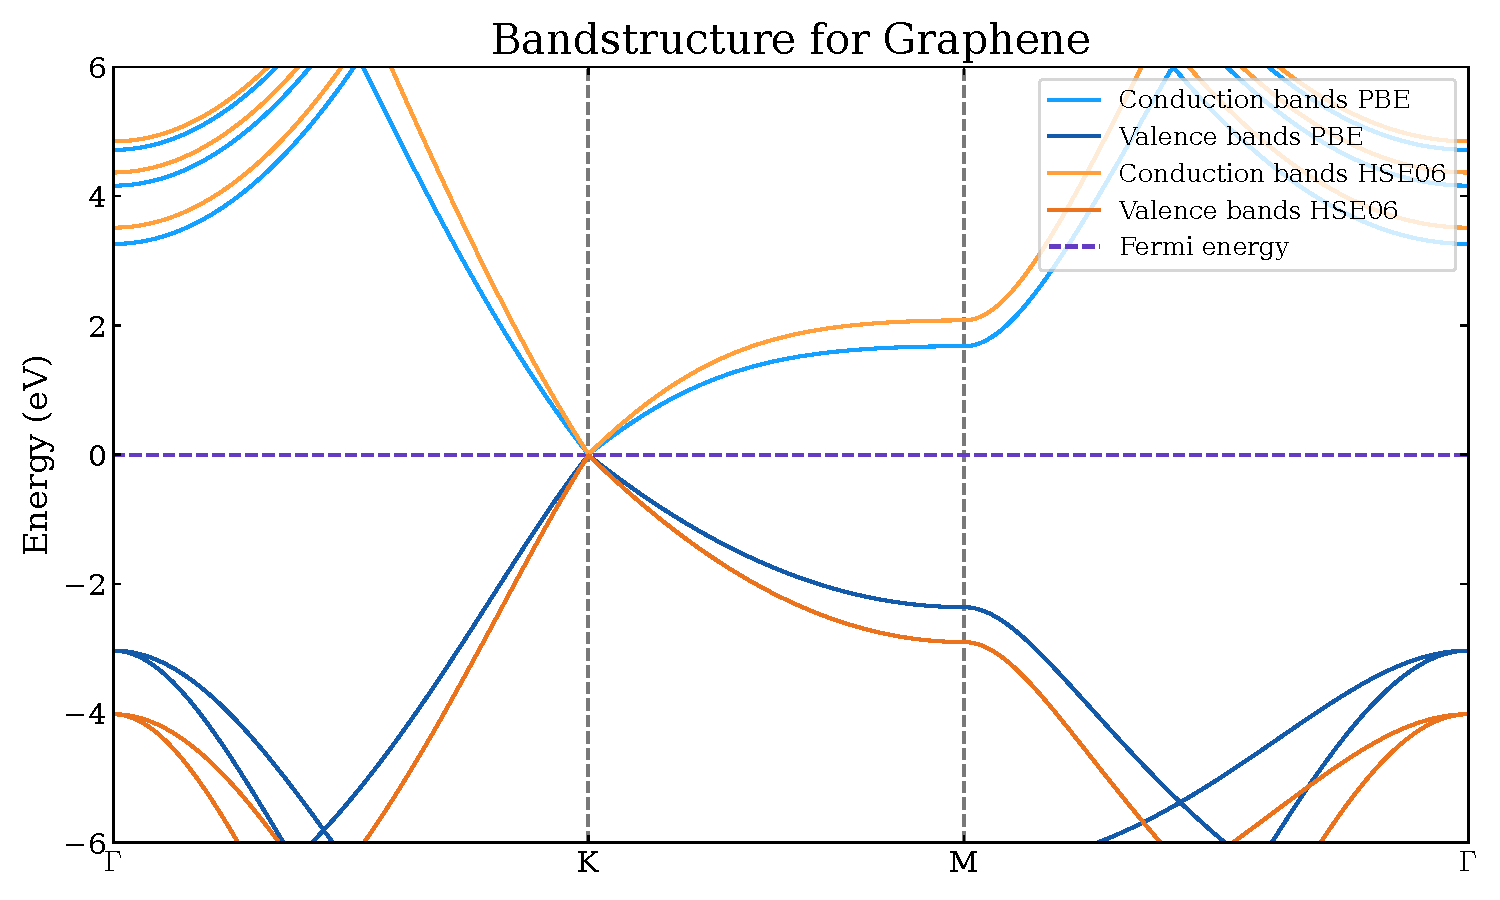
\includegraphics[width=0.40\textwidth]{figures_proj1/proj1.3a.pdf}%
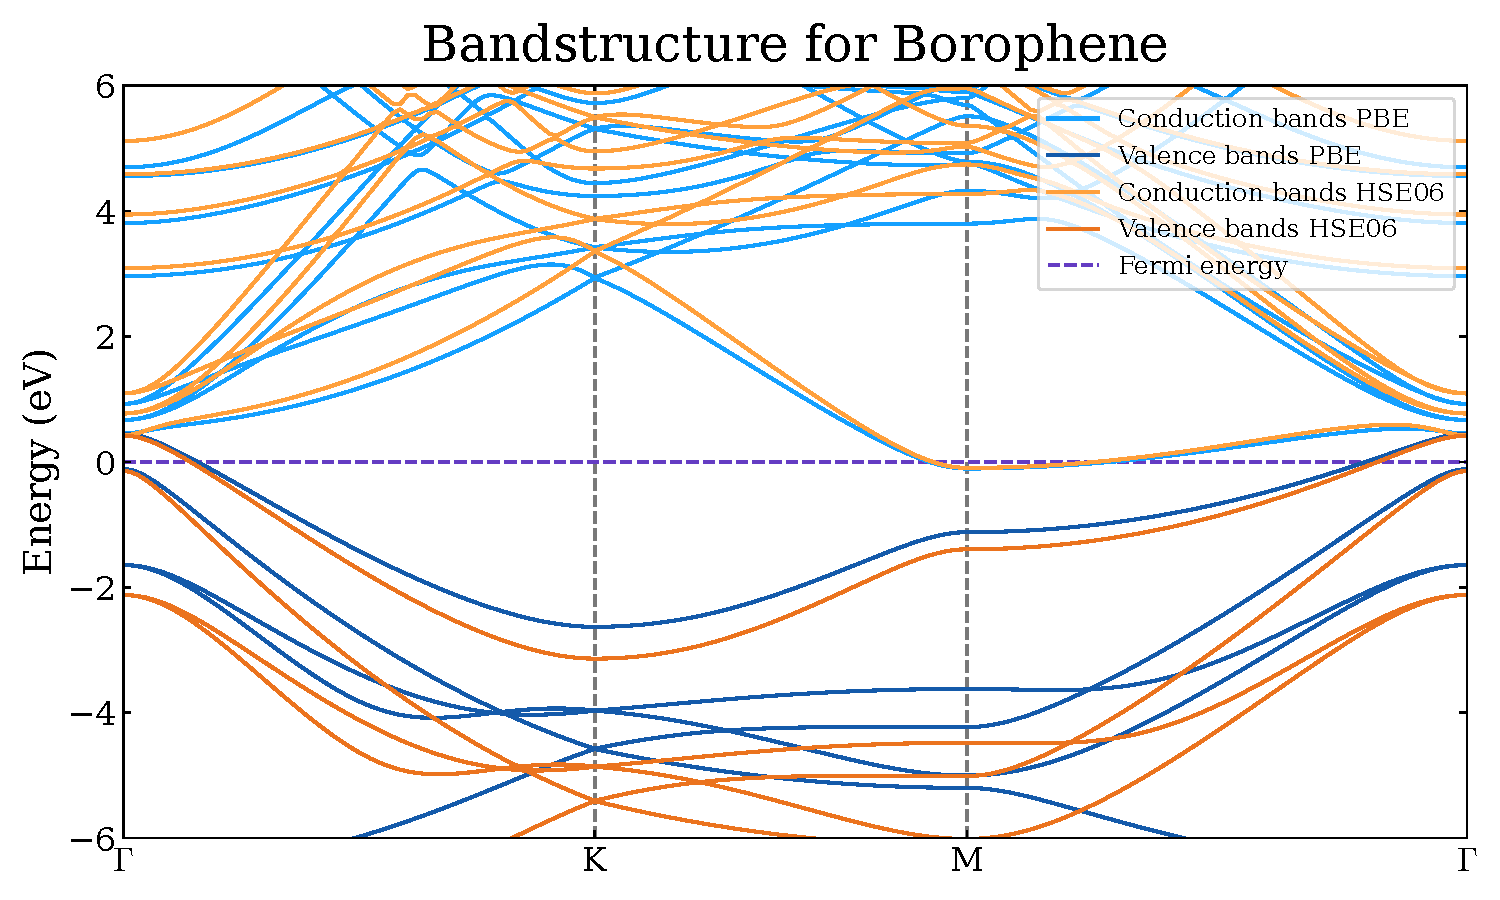
\includegraphics[width=0.40\textwidth]{figures_proj1/proj1.3b.pdf}%
\par\nointerlineskip
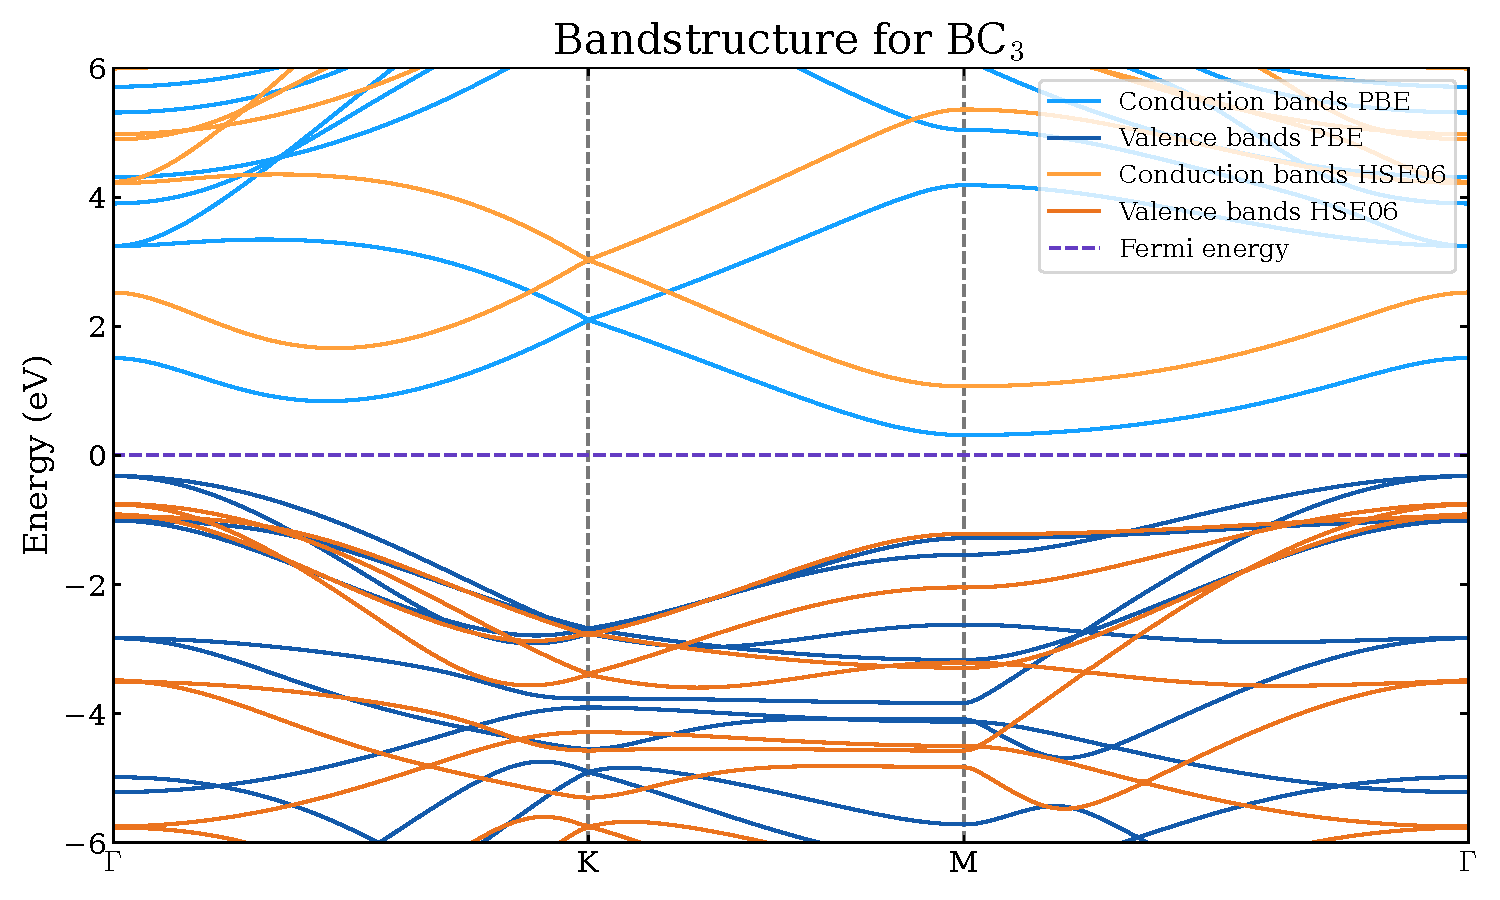
\includegraphics[width=0.40\textwidth]{figures_proj1/proj1.3c.pdf}%
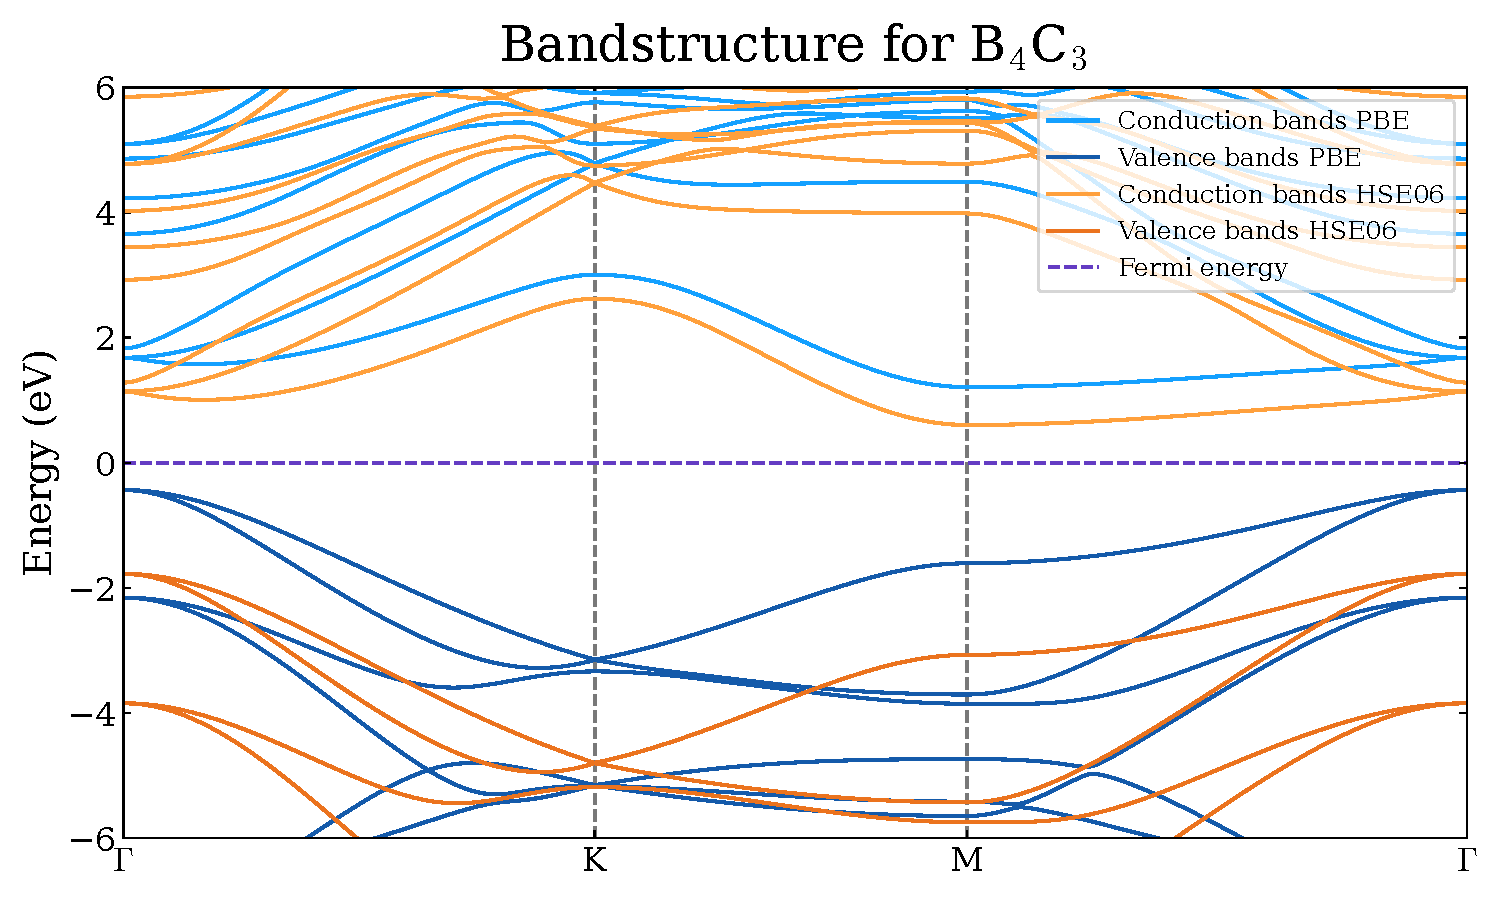
\includegraphics[width=0.40\textwidth]{figures_proj1/proj1.3d.pdf}%
\caption{Band structures of graphene, borophene, \ce{BC3}, and \ce{B4C3} calculated using PBE (blue) and HSE06 (orange).}
\label{fig1.2_monolayers_bs}
\end{figure}

\subsection{Heterostructure}

\subsubsection{Structural properties}

We next determine the structures of the bilayer heterojunctions,
which consist of monolayer graphene stacked with monolayer \ce{BC3}, borophene,
and \ce{B4C3}, namely Graphene-\ce{BC3}, Graphene-Borophene, and Graphene-\ce{B4C3}, respectively.
To create the heterostructures, we use a $2\times 2\times 1$ cell.
For each system,
we consider several lateral stacking coordinations of these layers.
Specifically, we consider ``Hollow'', ``Bridge'', and ``Top'' coordinations for the Graphene-\ce{BC3} bilayer system,
and ``Hollow 1'', ``Hollow 2'', ``Bridge'', and ``Top'' coordinations for the Graphene-Borophene and Graphene-\ce{B4C3} bilayer systems.
We calculate the relative energies,
optimized lattice constants, and interlayer distances for all structures.
Figures~\ref{S1.3}--\ref{S1.6} give details of this procedure.
Due to the weak van der Waals interaction between the layers,
the energy differences among the lateral positions are very small,
as shown in table~\ref{tab:S1.1}.

The results show that the lowest-energy lateral position for the Graphene-\ce{BC3} system is the ``Hollow'' stacking configuration.
As shown in figure~\ref{fig1.3},
each atom in \ce{BC3} projects to the centre of a hexagon in graphene.
Both the Graphene-Borophene and Graphene-\ce{B4C3} bilayer systems favour the ``Top'' stacking configuration.
In this arrangement, each atom-free hexagon in the bottom layer projects to the centre of a hexagon in graphene.
However, the converse does not hold, because not every hexagon centre in graphene aligns with an atom-free hexagon in the bottom layer, as illustrated in figure~\ref{fig1.3}.

\begin{figure}[!htbp]
\centering

\includegraphics[width=0.80\textwidth]{figures_proj1/proj1.3.pdf}
\caption{Top views of the optimized atomic structures of Graphene-\ce{BC3}, Graphene-Borophene, and Graphene-\ce{B4C3}.
Green and brown spheres denote boron and carbon atoms, respectively.
The orange parallelogram indicates the unit cell.}
\label{fig1.3}
\end{figure}

\begin{table}[!htbp]
\centering
\rowcolors{2}{gray!15}{white}
\begin{adjustbox}{max width=1.0\linewidth}
% \begin{tabular}{ccm{0.2\linewidth}m{0.18\linewidth}m{0.18\linewidth}m{0.18\linewidth}c}
\begin{tabular}{cccccccc}
\hline
\rowcolor{gray!25}
system
& coordination
& $a$ $(a=b)$ (Å)
& $S_{\mathrm{G}}$
& $S_{\mathrm{BC}/\mathrm{B}}$
& $d_{\mathrm{IL}}$ (Å)
& $E_{\mathrm{b}}$ (meV/atom)
& Nature \\ \hline

Graphene-\ce{BC3}
& Hollow
& 5.044
& \qty{2.23}{\percent}
& \qty{-2.42}{\percent}
& 3.375 % 3.372
& $-25.6$
& semimetal \\

Graphene-Borophene
& Top
& 4.979
& \qty{0.91}{\percent}
& \qty{-1.43}{\percent}
& 3.496 % 3.505
& $-24.2$
& metallic \\

Graphene-\ce{B4C3}
& Top
& 4.846
& \qty{-1.78}{\percent}
& \qty{3.33}{\percent}
& 3.514
& $-21.2$
& semimetal
\\ \hline
\end{tabular}
\end{adjustbox}
\caption{Optimized structural properties of each bilayer heterojunction system,
including the lowest-energy lateral stacking coordination relative to graphene,
the optimized lattice constant $a$,
the strains relative to the respective monolayers, $S_{\mathrm{G}}$ and $S_{\mathrm{BC}/\mathrm{B}}$,
the interlayer distance $d_{\mathrm{IL}}$,
the interlayer binding energy per atom $E_{\mathrm{b}}$ from equation~\eqref{interlayer_binding_energy},
and the electronic nature.
Negative and positive percentage strains denote compressive and tensile strains, respectively.}
\label{tab:1.2_heterostructure}
\end{table}

Table~\ref{tab:1.2_heterostructure} shows that Graphene-Borophene is metallic,
whereas Graphene-\ce{BC3} and Graphene-\ce{B4C3} are semimetals.
The interlayer binding energies of Graphene-\ce{BC3}, Graphene-Borophene, and Graphene-\ce{B4C3} are \qty{-25.6}{\milli\electronvolt}, \qty{-24.2}{\milli\electronvolt}, and \qty{-21.2}{\milli\electronvolt} per atom, respectively.
Among all heterostructure systems, \ce{B4C3} shows the largest tensile strain of \qty{3.33}{\percent}.
For Graphene-\ce{BC3},
graphene is under tensile strain and \ce{BC3} is under compressive strain.
For Graphene-Borophene,
graphene has a slight tensile strain,
while borophene experiences compressive strain.
For Graphene-\ce{B4C3},
graphene is under compressive strain,
while \ce{B4C3} is under a larger tensile strain.
In general, tensile strain tends to narrow the band gap and increase conductivity~\cite{roldan2015strain}.
Conversely, compressive strain tends to widen the band gap and decrease conductivity~\cite{boukhvalov2008hydrogen}.

\subsubsection{Charge-density difference}

The charge-density difference distributions of the heterostructure systems are shown in figure~\ref{fig1.4_cdd}.
We calculate these distributions using equation~\eqref{charge_density_difference}.
Specifically, we subtract the charge densities of the isolated monolayers from the charge density of the corresponding heterostructure.

\begin{figure}[!htbp]
\centering
    \includegraphics[width=1.00\textwidth]{figures_proj1/proj1.4.pdf}
\caption{Charge-density difference ($\Delta \rho(\vec{r}\,)$, calculated using equation~\eqref{charge_density_difference}) between the monolayers and the heterostructures.
Regions of charge accumulation are shown in yellow,
and regions of charge depletion are shown in blue.
The isosurface level is $1.5\times10^{-4}$ a$_{0}^{-3}$ and the top layer is always graphene.}
\label{fig1.4_cdd}
\end{figure}

The side views in the middle panels of figure~\ref{fig1.4_cdd} show charge depletion from the graphene layer and charge accumulation in the corresponding non-graphene monolayer for all three systems.
Among these systems, Graphene-\ce{BC3} exhibits the largest charge redistribution.
This larger charge redistribution is consistent with the smaller interlayer distance associated with the hollow-site coordination.
In contrast, Graphene-Borophene and Graphene-\ce{B4C3} adopt top-site coordination.

We also observe that atoms in the lower layers
that directly coordinate with a carbon atom in the graphene layer
have the largest charge accumulation regions.
In contrast, the carbon atoms in the graphene layer with bridge or hollow coordination to the atoms of the lower layer show the largest regions of charge depletion.
These coordination-dependent charge redistributions produce the accumulation and depletion patterns shown in the top and bottom views of figure~\ref{fig1.4_cdd}.
Therefore, the relative coordination of the two monolayers directly influences the interfacial electronic structure.
The top and bottom views of the Graphene-\ce{B4C3} heterostructure reveal a clear threefold rotational symmetry in the upper and lower plots of the rightmost panel.

In the next sections, we investigate the band structures and densities of states to further characterize the electronic structures of these heterostructure systems.

\subsubsection{Band structure and density of states}

For the bilayer systems, the band structures and total density of states (DoS) are shown in figures~\ref{fig1.5}--\ref{fig1.7} as calculated using the HSE06 and PBE functionals.
The corresponding atom-projected (or partial) PDoS are presented in figures~\ref{S1.9}--\ref{S1.11}.

The Graphene-\ce{BC3} heterojunction exhibits a sizeable density of states just above the Fermi level, as shown in figure~\ref{S1.10},
which is related to the relatively flat band near the $\mathrm{M}$ point and along the $\mathrm{K}$--$\Gamma$ path in the Brillouin zone.
The Graphene-Borophene system exhibits metallic behaviour,
with contributions from both constituent layers near the Fermi level, as shown by the PDoS in figure~\ref{S1.9}.
The Graphene-\ce{B4C3} bilayer exhibits essentially semimetallic behaviour, with the \ce{B4C3}-derived states located away from the Fermi level, mainly above approximately \qty{1.2}{\electronvolt} and below approximately \qty{-0.8}{\electronvolt}, as shown by the PDoS in figure~\ref{S1.11}.

Across these three bilayers,
HSE06 mainly shifts the conduction bands upward and the valence bands downward relative to PBE.
At the $\mathrm{K}$ point, the graphene bands exhibit very small band-gap openings of \qty{20}{\milli\electronvolt} and
\qty{50}{\milli\electronvolt} for Graphene-\ce{B4C3} and Graphene-\ce{BC3}, respectively.

Figures~\ref{fig1.5}--\ref{fig1.7} show the band structures and total DoS of the three bilayer systems calculated using the PBE and HSE06 functionals.
In each figure, the PBE and HSE06 results are shown in blue and orange, respectively, and the Fermi level is indicated by the purple dashed line.

\begin{figure}[!htbp]
\centering
    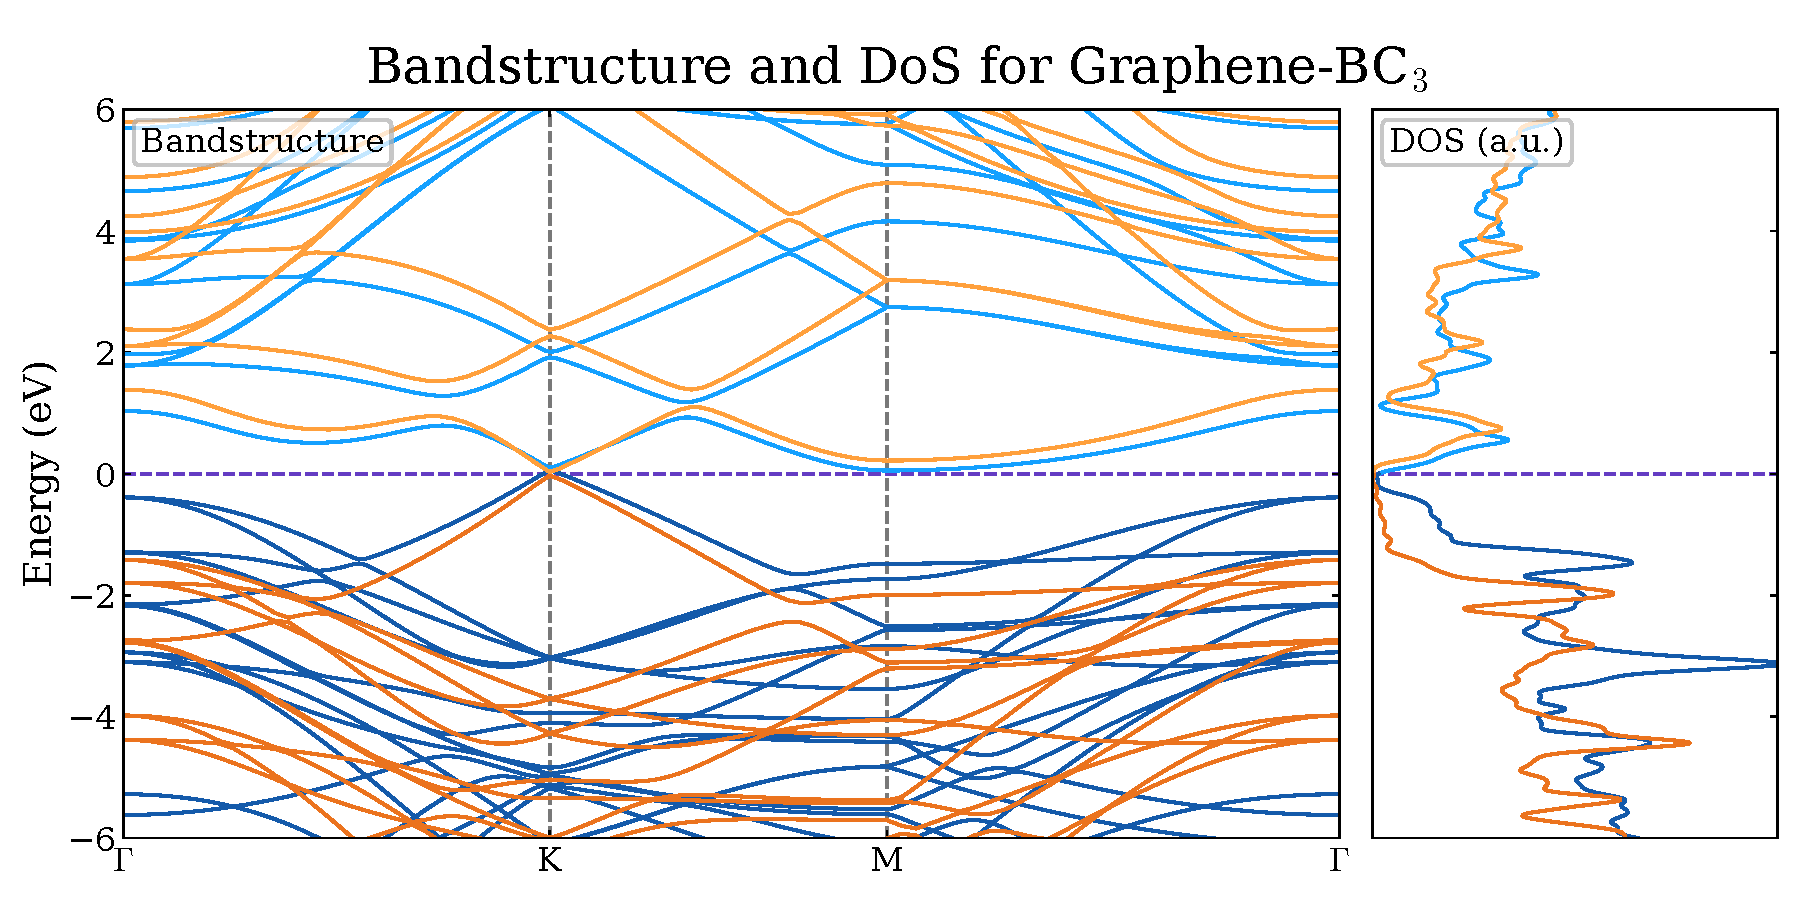
\includegraphics[width=0.80\textwidth]{figures_proj1/proj1.5.pdf}
\caption{Band structure and total DoS of Graphene-\ce{BC3}.}
\label{fig1.5}
\end{figure}

\begin{figure}[!htbp]
\centering
    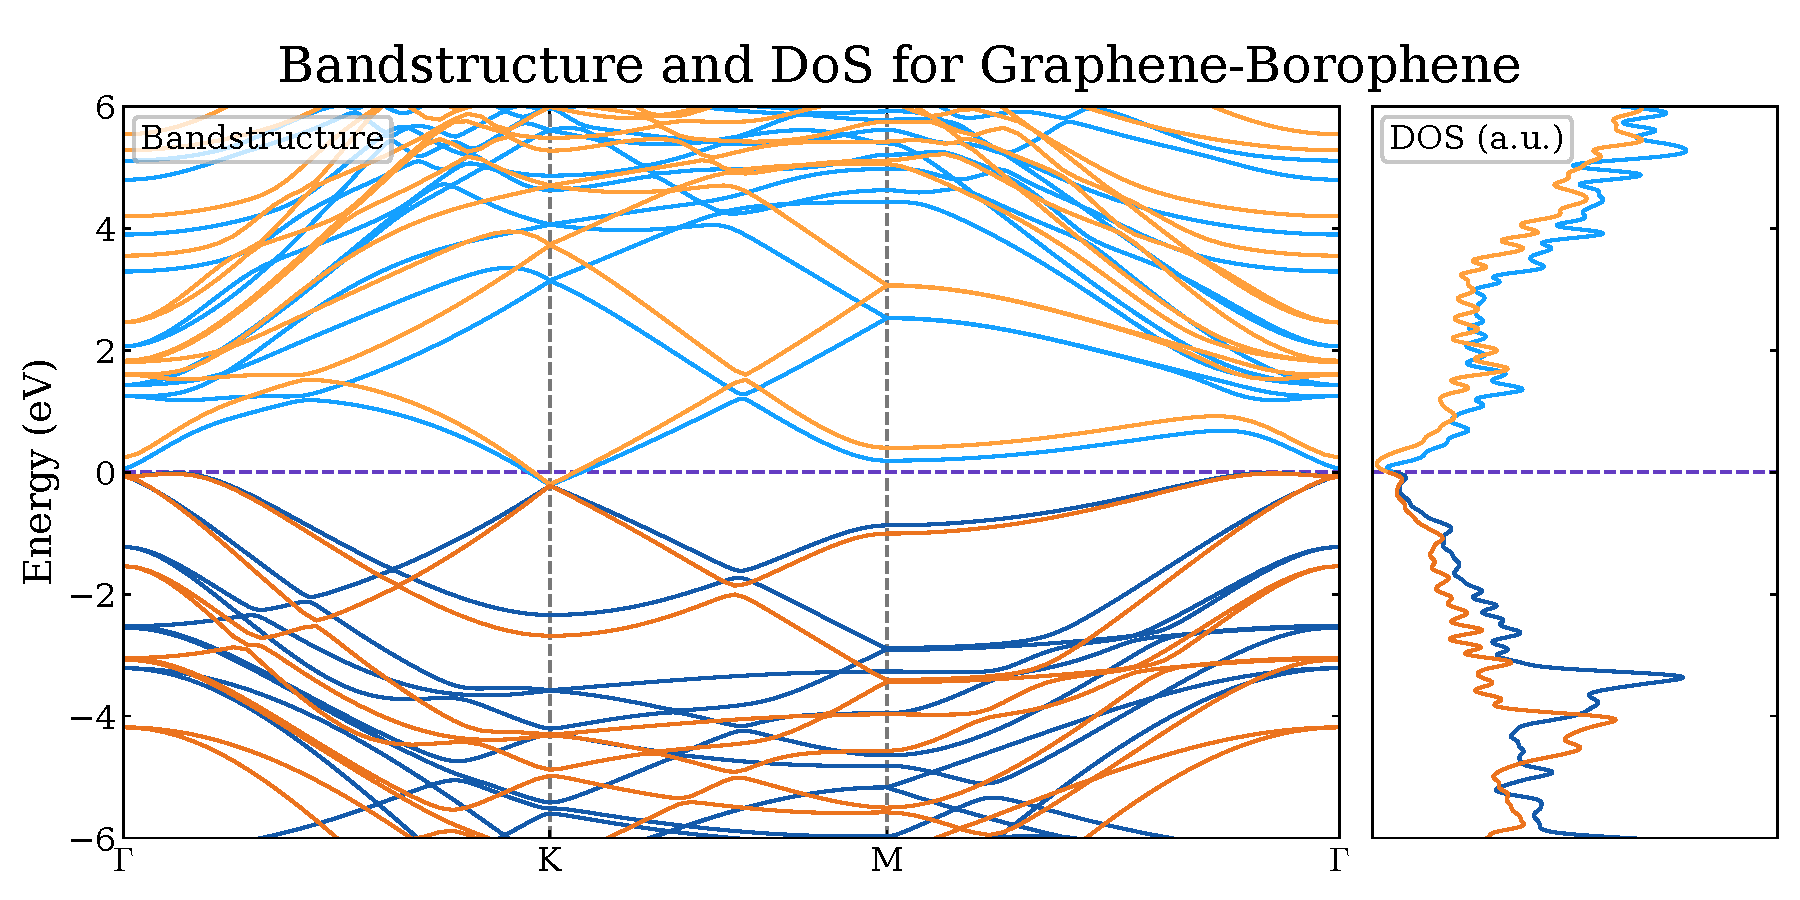
\includegraphics[width=0.80\textwidth]{figures_proj1/proj1.6.pdf}
\caption{Band structure and total DoS of Graphene-Borophene.}
\label{fig1.6}
\end{figure}

\begin{figure}[!htbp]
\centering
    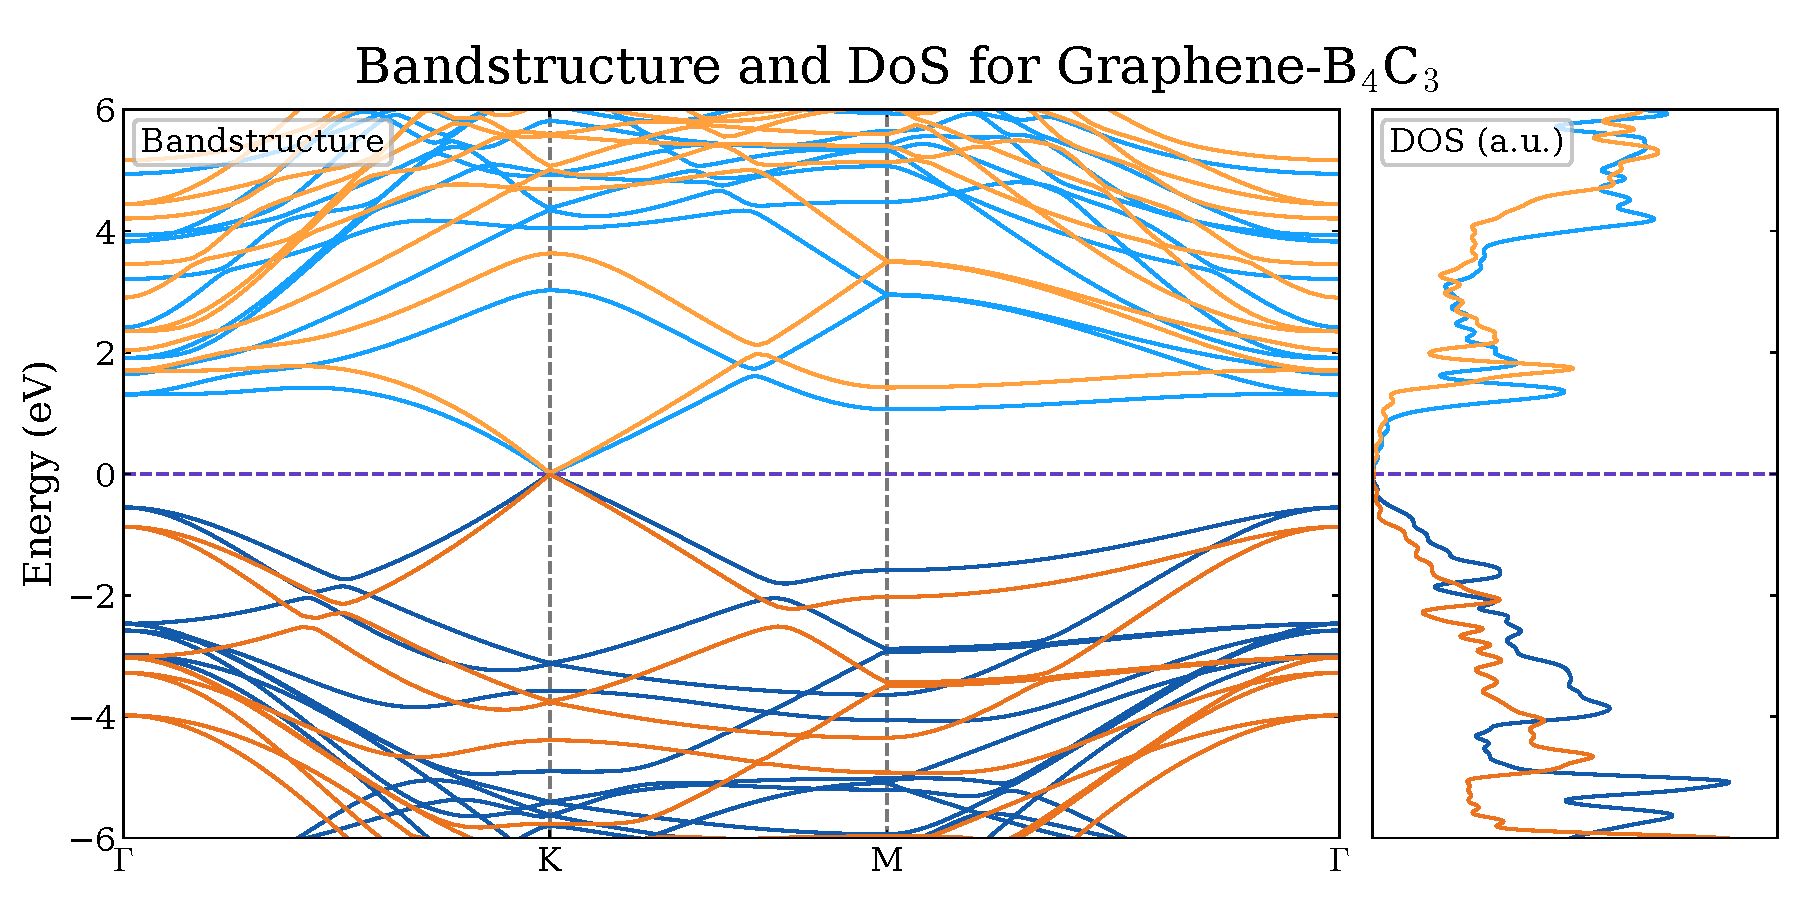
\includegraphics[width=0.80\textwidth]{figures_proj1/proj1.7.pdf}
\caption{Band structure and total DoS of Graphene-\ce{B4C3}.}
\label{fig1.7}
\end{figure}

\subsubsection{Schottky barrier height}

Bilayer heterostructures composed of graphene and boron-carbide monolayers can function as Schottky diodes.
A high Schottky barrier blocks the reverse current from the metal to the semiconductor and enables the rectification effect of a diode.
Based on the Schottky--Mott model shown in figure~\ref{fig1.8},
the Schottky barrier at a metal-semiconductor interface~\cite{guo2017all} is determined by the relative positions of the Fermi level and the semiconductor band edges.

For $n$-type materials, the Schottky barrier $\Phi_\mathrm{n}$ is defined as the energy difference between the conduction band minimum $E_\mathrm{C}$ and the Fermi level $E_\mathrm{F}$:

\begin{equation}
    \Phi_\mathrm{n} = E_\mathrm{C} - E_\mathrm{F}
\end{equation}

Similarly, for $p$-type materials, the Schottky barrier $\Phi_\mathrm{p}$ is defined as the energy difference between the Fermi level $E_\mathrm{F}$ and the valence band maximum $E_\mathrm{V}$:

\begin{equation}
    \Phi_\mathrm{p} = E_\mathrm{F} - E_\mathrm{V}
\end{equation}

The sum of these two Schottky barriers is approximately equal to the semiconductor band gap $E_\mathrm{g}$:

\begin{equation}
    \Phi_\mathrm{n} + \Phi_\mathrm{p} \approx E_\mathrm{g}
\end{equation}

For the Graphene-\ce{B4C3} system illustrated in figure~\ref{fig1.8}, we find $\Phi_\mathrm{n} = \qty{1.42}{\electronvolt}$ ($\qty{1.07}{\electronvolt}$) and $\Phi_\mathrm{p} = \qty{0.87}{\electronvolt}$ ($\qty{0.55}{\electronvolt}$) using HSE06 (PBE).
Since $\Phi_\mathrm{p} < \Phi_\mathrm{n}$, this heterojunction forms a $p$-type Schottky barrier.
For the Graphene-\ce{BC3} heterostructure bilayer, we find $\Phi_\mathrm{n} = \qty{0.19}{\electronvolt}$ ($\qty{0.003}{\electronvolt}$) and $\Phi_\mathrm{p} = \qty{1.42}{\electronvolt}$ ($\qty{0.39}{\electronvolt}$) using HSE06 (PBE).
This result indicates that the Graphene-\ce{BC3} heterojunction forms an $n$-type Schottky barrier.
For device applications, a smaller Schottky barrier height, or even an Ohmic contact, is preferred to reduce contact resistance.

\begin{figure}[!htbp]
\centering
    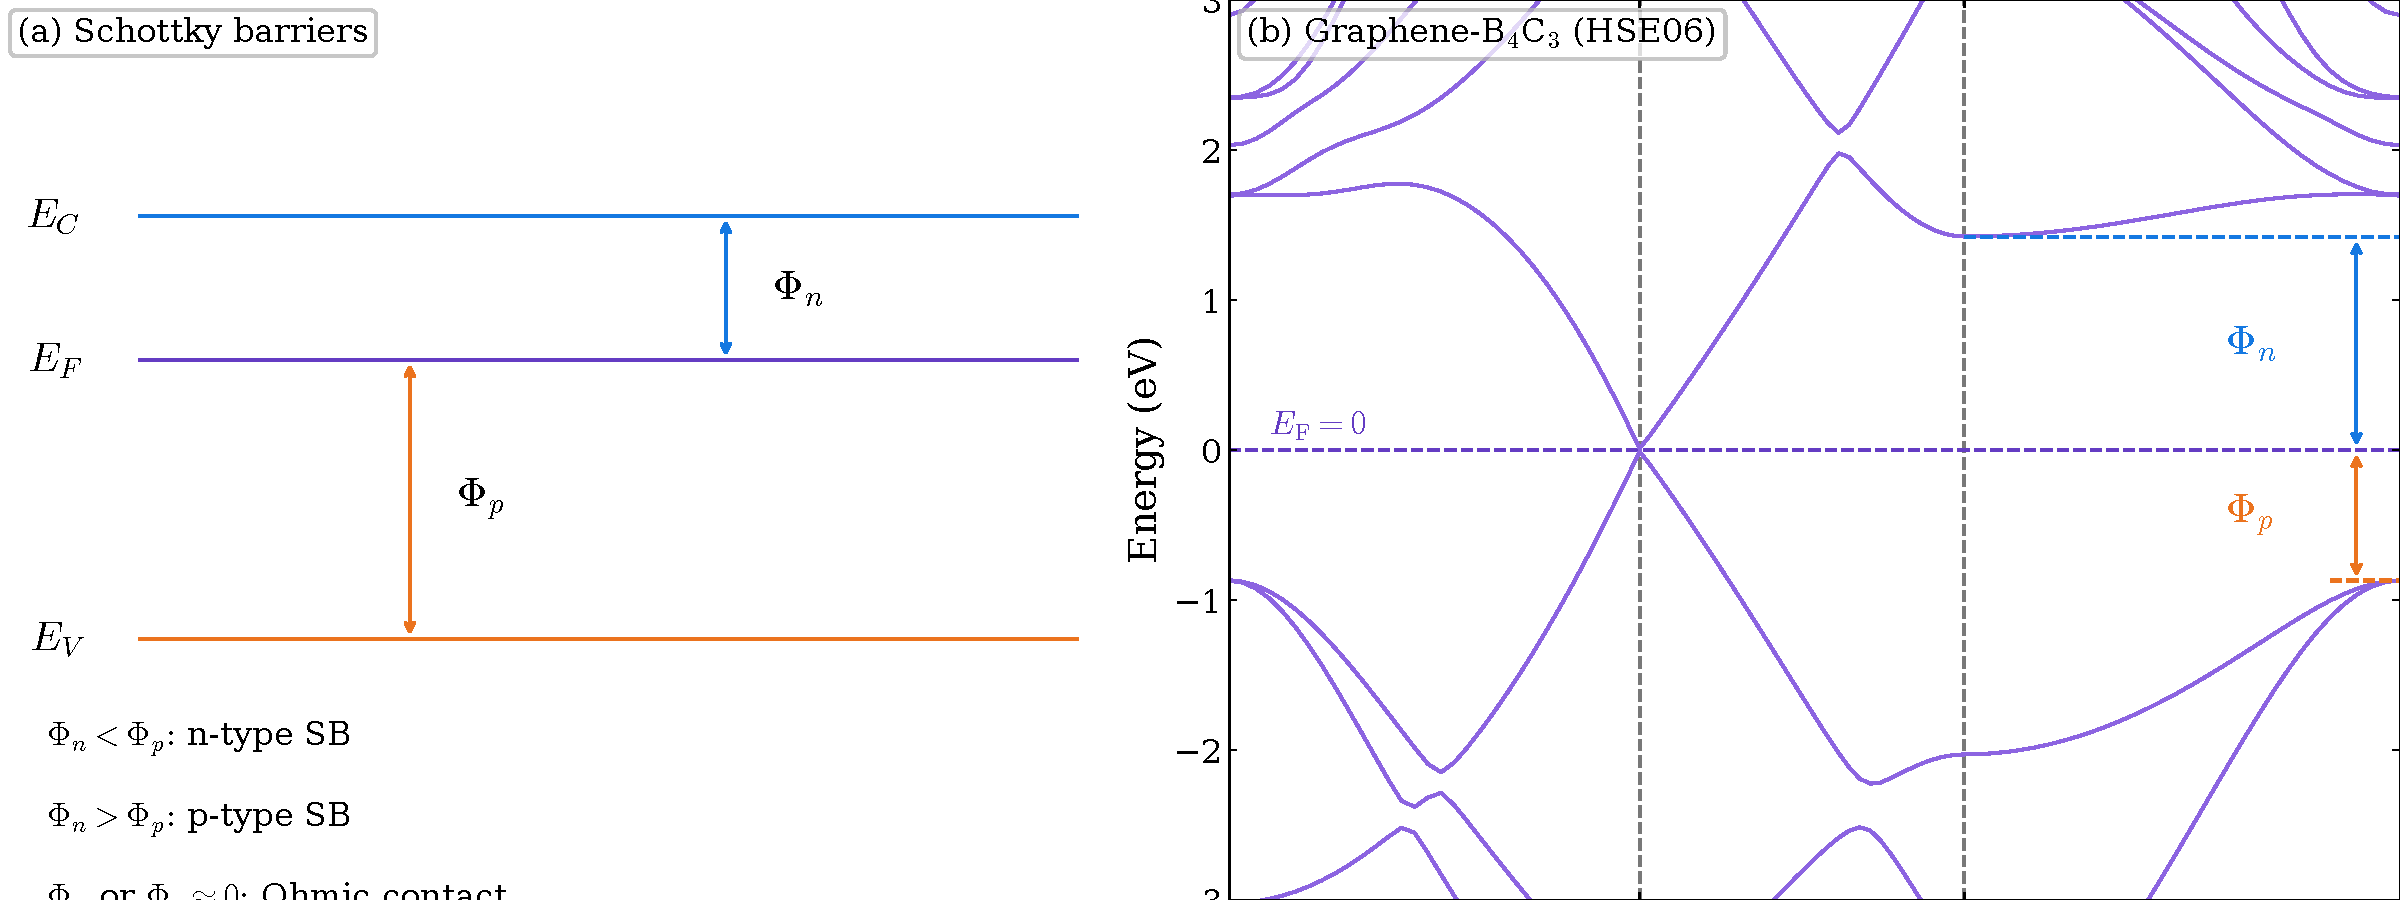
\includegraphics[width=0.80\textwidth]{figures_proj1/proj1.8_schottky.pdf}
\caption{Panel~(a) shows a schematic of the Schottky--Mott model, including the valence and conduction band energies, the Fermi energy, and the $n$-type and $p$-type Schottky barriers labelled $E_\mathrm{V}$, $E_\mathrm{C}$, $E_\mathrm{F}$, $\Phi_\mathrm{n}$, and $\Phi_\mathrm{p}$, respectively; panel~(b) shows an example of the HSE06-calculated Graphene-\ce{B4C3} heterojunction and the Schottky barrier height determined from the band structure.}
\label{fig1.8}
\end{figure}

\subsection{Dielectric function}

Having determined the atomic and electronic properties of the bilayer systems,
we calculate the real part $\varepsilon_1$ and imaginary part $\varepsilon_2$ of the dielectric function,
from which the other optical properties can be determined, as given by equations~\eqref{absorption_coefficient_from_dielectric_function},
\eqref{refractive_index_from_dielectric_response},
\eqref{extinction_coefficient_from_dielectric_response},
\eqref{reflectivity_from_refractive_index_and_extinction_coefficient},
and~\eqref{energy_loss_spectrum_from_inverse_dielectric_function}.
The real part of the frequency-dependent dielectric function $\varepsilon_1(\omega)$ characterizes the strength of the dynamical screening from charge excitations,
whereas the imaginary part $\varepsilon_2(\omega)$ describes the absorptive response.
A negative value of $\varepsilon_1(\omega)$ indicates metallic character in the optical response over the corresponding photon-energy range.
A plasmon assignment further requires a corresponding peak in the energy-loss spectrum, with sufficiently weak damping near the zero crossing of $\varepsilon_1$.
The plasmon-related features discussed below are interpreted within this long-wavelength dielectric description.
Their dispersion and lifetimes are not calculated here.

It is first important to establish the appropriate k-point set to yield converged results.
For graphene, we test a number of k-point meshes and find that a $129 \times 129 \times 1$ mesh gives converged results, as shown in figure~\ref{S1.12}, in good agreement with previous results~\cite{warmbier2016}.
We therefore use this k-point sampling density for the other single monolayers, whose unit cells are $2 \times 2$ relative to graphene, namely a $65 \times 65 \times 1$ k-point mesh.
The dielectric functions for all the monolayers are shown in figure~\ref{S1.13}, where the results are consistent with previous calculations, namely graphene~\cite{warmbier2016}, \ce{BC3}~\cite{chen2019plasmon,mortazavi2019outstanding}, \ce{B4C3}~\cite{chang2019b4c3}, and borophene~\cite{huang2017,li2017first}.

The anisotropic in-plane and out-of-plane components of the dielectric function show that the optical response depends strongly on the polarization direction of the incoming light.
For the in-plane direction, the well-known $\pi$ plasmon of graphene emerges around \qty{4}{\electronvolt},
and the $\pi-\sigma$ plasmon emerges around \qty{14}{\electronvolt}.
The other monolayer systems also have a $\pi$-like plasmon,
which emerges for \ce{B4C3} around \qty{3}{\electronvolt},
for \ce{BC3} around \qty{2}{\electronvolt},
and for borophene around \qty{1}{\electronvolt}.
It can furthermore be seen from figure~\ref{S1.13} that, for the real part of the dielectric function in the out-of-plane direction for borophene,
the real part becomes negative at approximately \qty{9.8}{\electronvolt} and positive again around \qty{10.5}{\electronvolt},
suggesting a possible plasmonic feature.

As previously reported, the latter three monolayers exhibit visible-light absorption,
which is also indicated by the in-plane imaginary part of the dielectric function shown in figure~\ref{S1.13}.
The static dielectric constants, namely the real part of the dielectric function at zero energy,
for \ce{BC3} are approximately 4.1 for in-plane polarization and 1.4 for out-of-plane polarization as obtained using PBE.
These values can be compared with previously reported PBE values of 4.86 for in-plane polarization and 1.59 for out-of-plane polarization~\cite{mortazavi2019outstanding}.

For \ce{B4C3}, the in-plane static dielectric constant is approximately 3.8,
and the out-of-plane value is calculated to be 1.5.
We note that these values reflect the combined monolayer-vacuum system.
Figure~\ref{S1.14} shows the corresponding optical properties for the monolayer systems.

Before presenting the results for the three heterostructure bilayer systems,
we first perform a convergence check for the total number of bands, including unoccupied states, used to calculate the dielectric function.
Figure~\ref{S1.15} shows that an input value of \texttt{NBANDS=128} yields well-converged results for the representative Graphene-\ce{B4C3} system,
and we therefore use this input value for all three bilayer calculations.
Further tests of the energy convergence criterion are reported in figure~\ref{S1.16}.

% Graphene-Borophene
The results for the dielectric function of the Graphene-Borophene heterojunction are shown in figure~\ref{fig1.9},
as obtained using both the PBE and HSE06 functionals.
The corresponding full dielectric tensor components are provided in figure~\ref{S1.17}.
Compared with the PBE results,
HSE06 yields a blue shift of the features to higher energies.
The real part exhibits characteristics of both graphene and borophene,
with negative values around the same energies as those of the respective monolayers shown in figure~\ref{S1.13},
namely around \qty{5}{\electronvolt} (\qty{4}{\electronvolt}) and \qty{2}{\electronvolt} (\qty{1}{\electronvolt}) for HSE06 (PBE), respectively.
There is, however, a significant difference in the out-of-plane dielectric function compared with the monolayer systems.
The borophene-related feature that emerges at around \qty{9.8}{\electronvolt} in the monolayer shifts to higher energies and now appears at around \qty{17}{\electronvolt} (\qty{14}{\electronvolt}) for HSE06 (PBE),
with a corresponding zero crossing at about \qty{18}{\electronvolt} (\qty{15}{\electronvolt}) for HSE06 (PBE),
where the real part of the dielectric function changes from negative to positive.
In addition, a new feature with two peaks occurs around \qtyrange{2}{5}{\electronvolt} (\qtyrange{1}{4}{\electronvolt}) for HSE06 (PBE) in both the real and imaginary parts of the dielectric function.
This feature in the imaginary part is attributed to interband transitions involving borophene- and graphene-derived states around the $\mathrm{K}$ point and along the direction towards the $\mathrm{M}$ and $\Gamma$ points.
A similar feature appears for the other bilayer heterojunctions, although it shows only one main peak.
For in-plane polarization, the first main peak of $\varepsilon_2$ occurs in the visible range and is related to $\pi-\pi^*$ transitions.
The main peaks along the out-of-plane direction are broad and occur in the energy range \qtyrange{9}{18.5}{\electronvolt} (\qtyrange{8}{17.5}{\electronvolt}) for HSE06 (PBE),
being related to $\pi-\sigma^*$ and $\pi^*-\sigma$ transitions.

\begin{figure}[!htbp]
\centering
    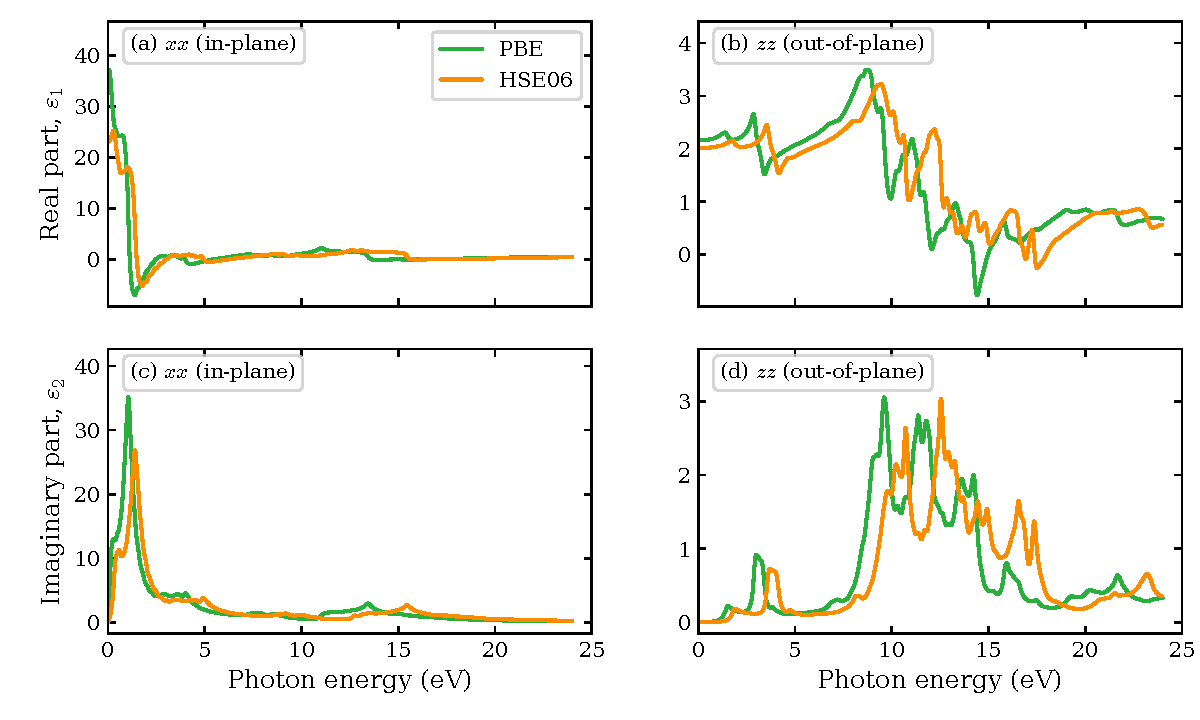
\includegraphics[width=0.80\textwidth]{figures_proj1/proj1.9.pdf}
\caption{In-plane and out-of-plane dielectric-function components of the Graphene-Borophene heterostructure.}
\label{fig1.9}
\end{figure}

% Graphene-BC3
The results for the dielectric function of the Graphene-\ce{BC3} heterostructure are shown in figure~\ref{fig1.10},
as obtained using both the PBE and HSE06 functionals.
The corresponding full dielectric tensor components are provided in figure~\ref{S1.18}.
Interestingly, and in contrast to Graphene-Borophene,
the displayed dielectric tensor for this system contains complex non-zero off-diagonal components.
The displayed off-diagonal pairs have approximately opposite signs:
$\varepsilon_{xy}\approx-\varepsilon_{yx}$,
$\varepsilon_{xz}\approx-\varepsilon_{zx}$,
and $\varepsilon_{yz}\approx-\varepsilon_{zy}$.
The dielectric tensor describes the response of a material to an external electric field,
or equivalently, how the polarization of the material changes under the applied electric field.
For an incident photon,
the tensor components describe the response of the material to the photon electric-field component along different directions.
For example, the elements $\varepsilon_{xy}$ and $\varepsilon_{yx}$ describe the coupling between the $x$ and $y$ directions,
namely the response to an electric field applied along one direction resulting in polarization along the other direction, and vice versa.
However, these off-diagonal components are mainly non-zero only in the low-energy region and remain small in magnitude.
In the symmetric tensor of the reciprocal response~\eqref{independent_particle_imaginary_dielectric_tensor}, the opposite-sign pairs cancel to below \qty{1}{\percent} of the diagonal components.
Therefore, the following discussion focuses on the in-plane and out-of-plane diagonal components,
which describe the dominant optical response for the polarization directions considered here.

In contrast to the Graphene-Borophene system,
the real part of the in-plane dielectric function is predominantly positive at low photon energies,
although small negative intervals are also present.
There are, however, energy ranges where it approaches zero,
namely in the region \qtyrange{2.5}{5}{\electronvolt} and from \qty{13}{\electronvolt} (\qty{15}{\electronvolt}) onwards for PBE (HSE06).
These near-zero values are considered together with $\varepsilon_2$ and the energy-loss spectrum,
which together determine the reflectivity and a possible plasmon resonance.
Another difference from the Graphene-Borophene system is the sizeable in-plane value of both $\varepsilon_1$ and $\varepsilon_2$ in the region \qtyrange{10}{15}{\electronvolt}.
Similar to the Graphene-Borophene system, however,
the out-of-plane real part of the dielectric function becomes negative at around \qtyrange{16}{17}{\electronvolt} (\qtyrange{14}{15}{\electronvolt}) for HSE06 (PBE),
consistent with the plasmon-like energy-loss feature discussed below.
However, monolayer \ce{BC3} does not exhibit this feature, unlike borophene, as shown in figure~\ref{S1.13}.
It is therefore presumably related to the $\pi-\sigma$-type plasmon present for graphene at approximately \qty{15}{\electronvolt},
but involves transitions between states associated with both monolayers.
For in-plane polarization, the first main peaks of $\varepsilon_2$ occur in the visible range and are related to $\pi-\pi^*$ transitions.
The main peaks along the out-of-plane direction are broad and occur in the energy range \qtyrange{11}{17}{\electronvolt} (\qtyrange{9}{16}{\electronvolt}) for HSE06 (PBE),
being related to $\pi-\sigma^*$ and $\pi^*-\sigma$ transitions.

\begin{figure}[!htbp]
\centering
    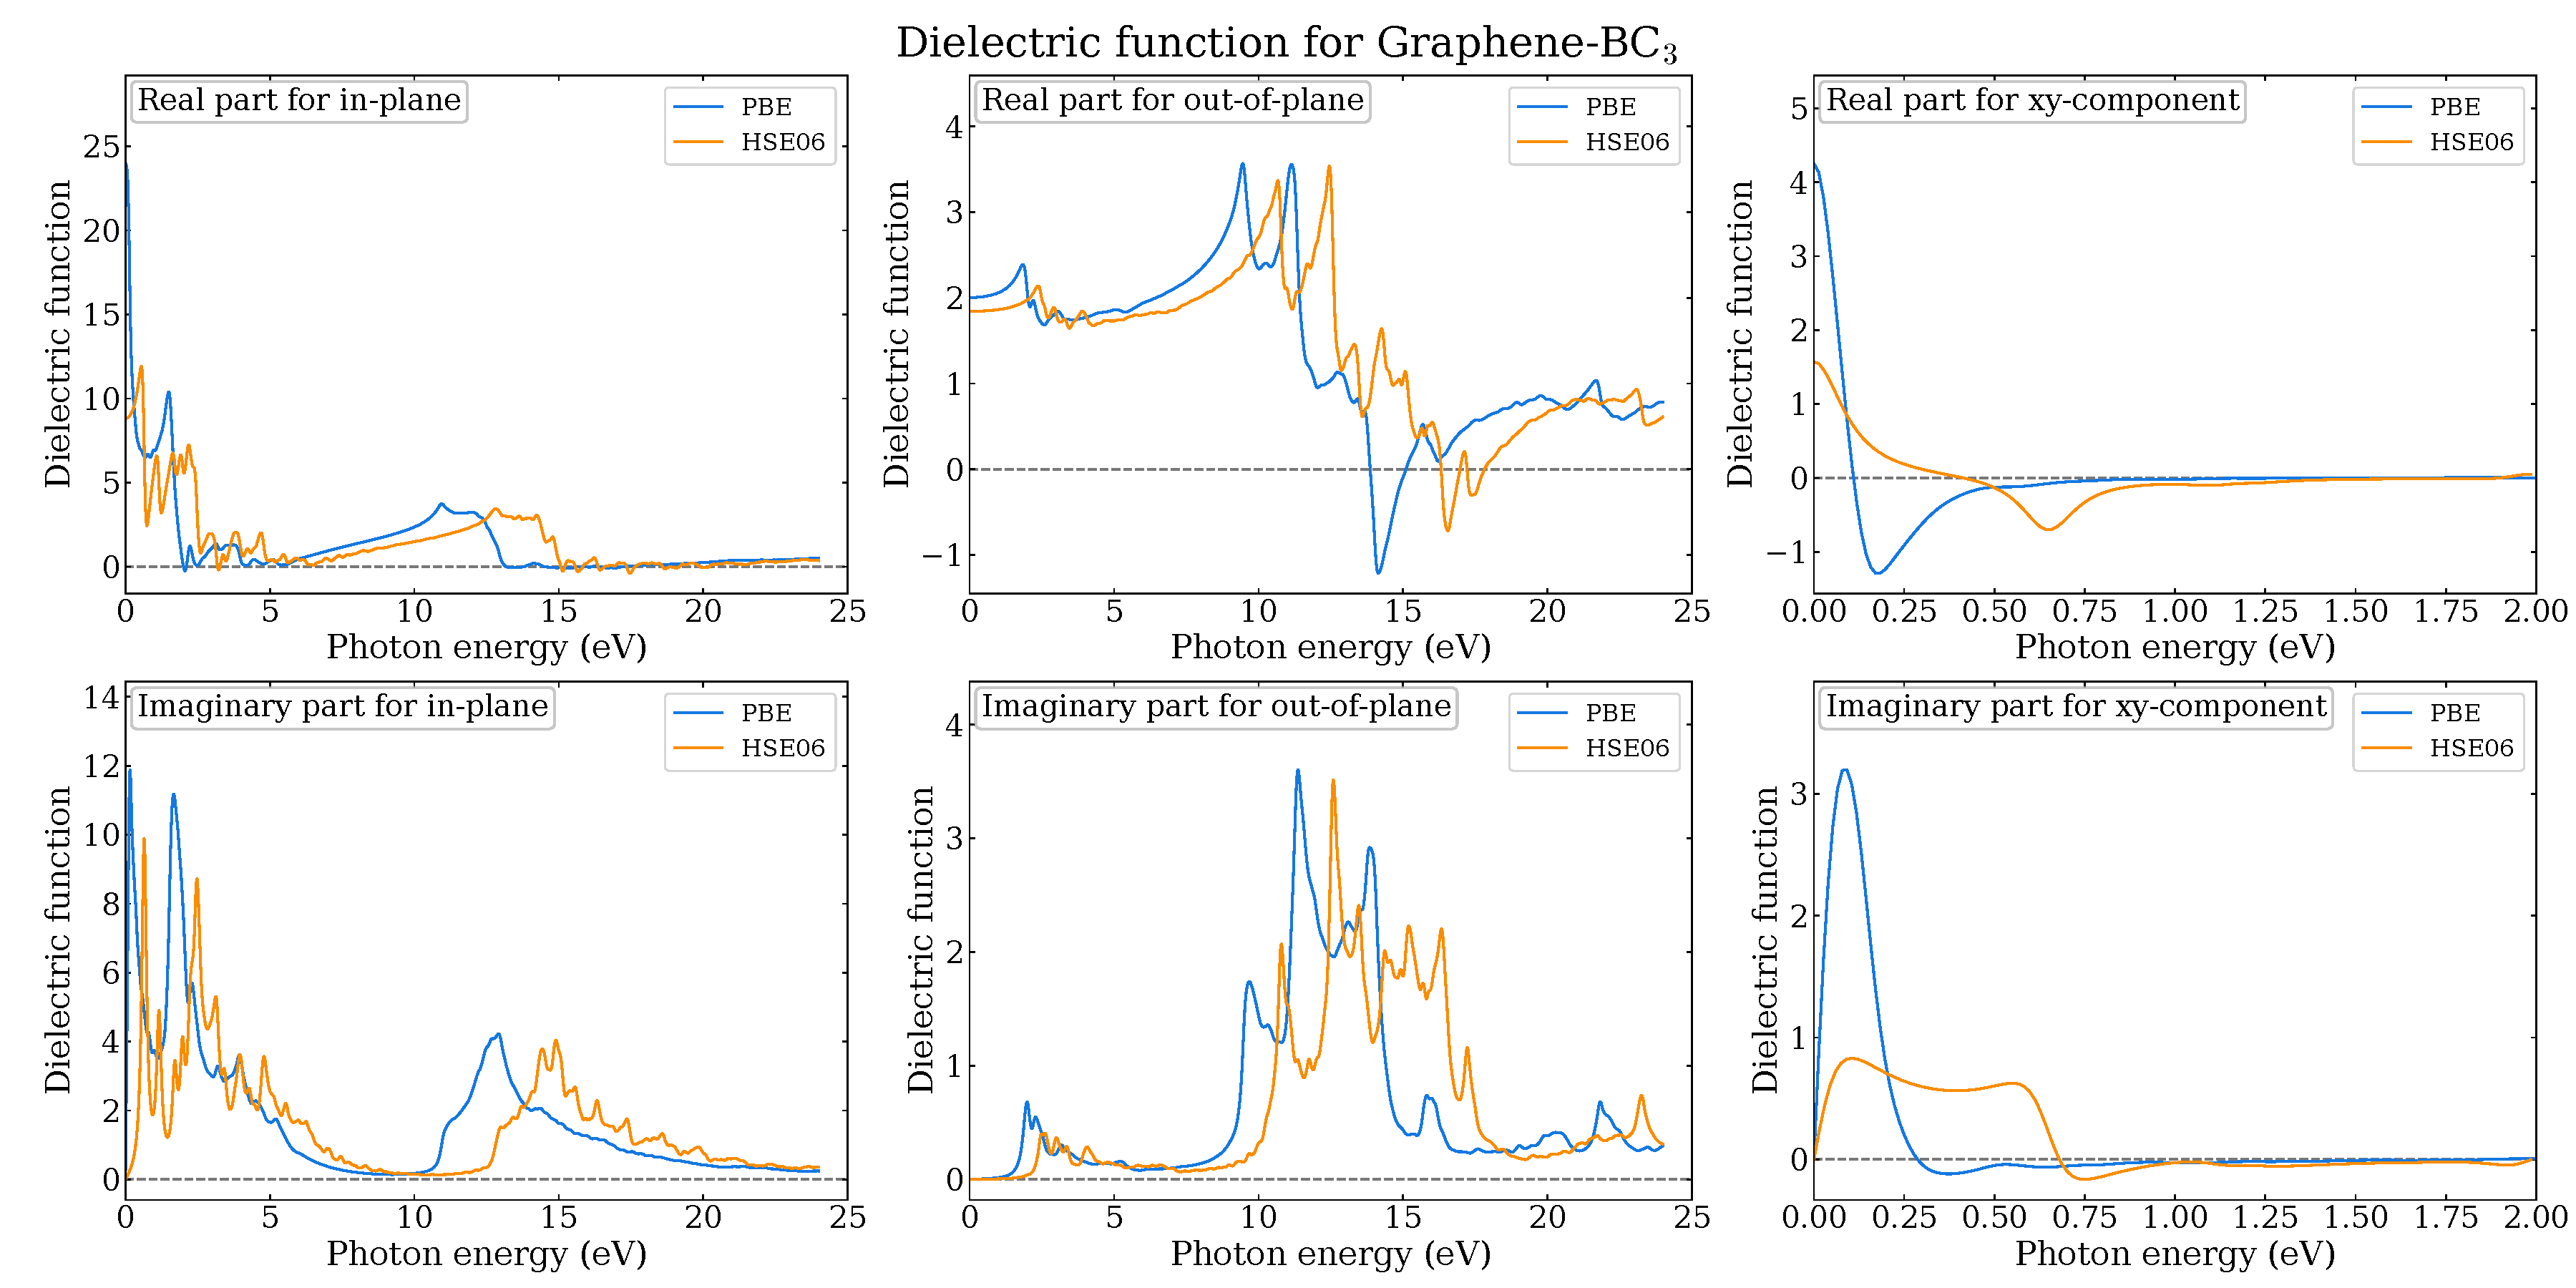
\includegraphics[width=1.00\textwidth]{figures_proj1/proj1.10_diff.pdf}
\caption{In-plane, out-of-plane, and off-diagonal $\varepsilon_{xy}$ components of the dielectric function for the Graphene-\ce{BC3} heterostructure.}
\label{fig1.10}
\end{figure}

% Graphene-B4C3
The results for the dielectric function of the Graphene-\ce{B4C3} heterostructure are shown in figure~\ref{fig1.11},
as obtained using both the PBE and HSE06 functionals.
The corresponding full dielectric tensor components are provided in figure~\ref{S1.19}.
The off-diagonal $\varepsilon_{xy}$ component is also included in figure~\ref{fig1.11}.
The real part of the in-plane dielectric function is negative in two regions:
\qtyrange{5}{6}{\electronvolt} for HSE06 (\qtyrange{4}{5}{\electronvolt} for PBE)
and \qtyrange{17}{18}{\electronvolt} for HSE06 (\qtyrange{15}{16}{\electronvolt} for PBE).
These negative regions must likewise be considered together with the ultraviolet energy-loss features.
The out-of-plane component also displays negative values at about \qtyrange{17}{18}{\electronvolt} for HSE06 (\qtyrange{14.5}{15.5}{\electronvolt} for PBE).

Similar to Graphene-\ce{BC3},
the first main peaks of $\varepsilon_2$ for in-plane polarization are also in the visible range.
The broad main peaks along the out-of-plane direction occur in the energy range \qtyrange{10}{18}{\electronvolt} (\qtyrange{9}{17}{\electronvolt}) for HSE06 (PBE).

The displayed dielectric tensor for this system also contains complex non-zero off-diagonal components.
The displayed off-diagonal pairs again have approximately opposite signs,
as shown in figure~\ref{S1.19}.
In contrast to Graphene-\ce{BC3}, however, these components remain non-zero over a considerable energy range,
namely from \qtyrange{0}{5}{\electronvolt} and from \qtyrange{10}{15}{\electronvolt}.
The original study assigns the system to the $\mathrm{P}3$ space group,
with threefold rotational symmetry along the $c$ axis, corresponding to the $z$ direction.
It also lacks mirror-symmetry planes perpendicular to this axis or within the $a,b$ plane,
corresponding to the $x,y$ plane.
For the reciprocal response in the local limit, threefold rotation about $z$ gives equal diagonal in-plane components and vanishing off-diagonal components~\cite{nye1985physical}.
In the symmetric part of the calculated tensor, the opposite-sign pairs in figure~\ref{S1.19} cancel, and both relations hold to within \qty{0.3}{\percent} of the diagonal components.
The difference between the diagonal in-plane and out-of-plane components nevertheless shows that Graphene-\ce{B4C3} dissipates energy differently for these two polarizations.

\begin{figure}[!htbp]
\centering
    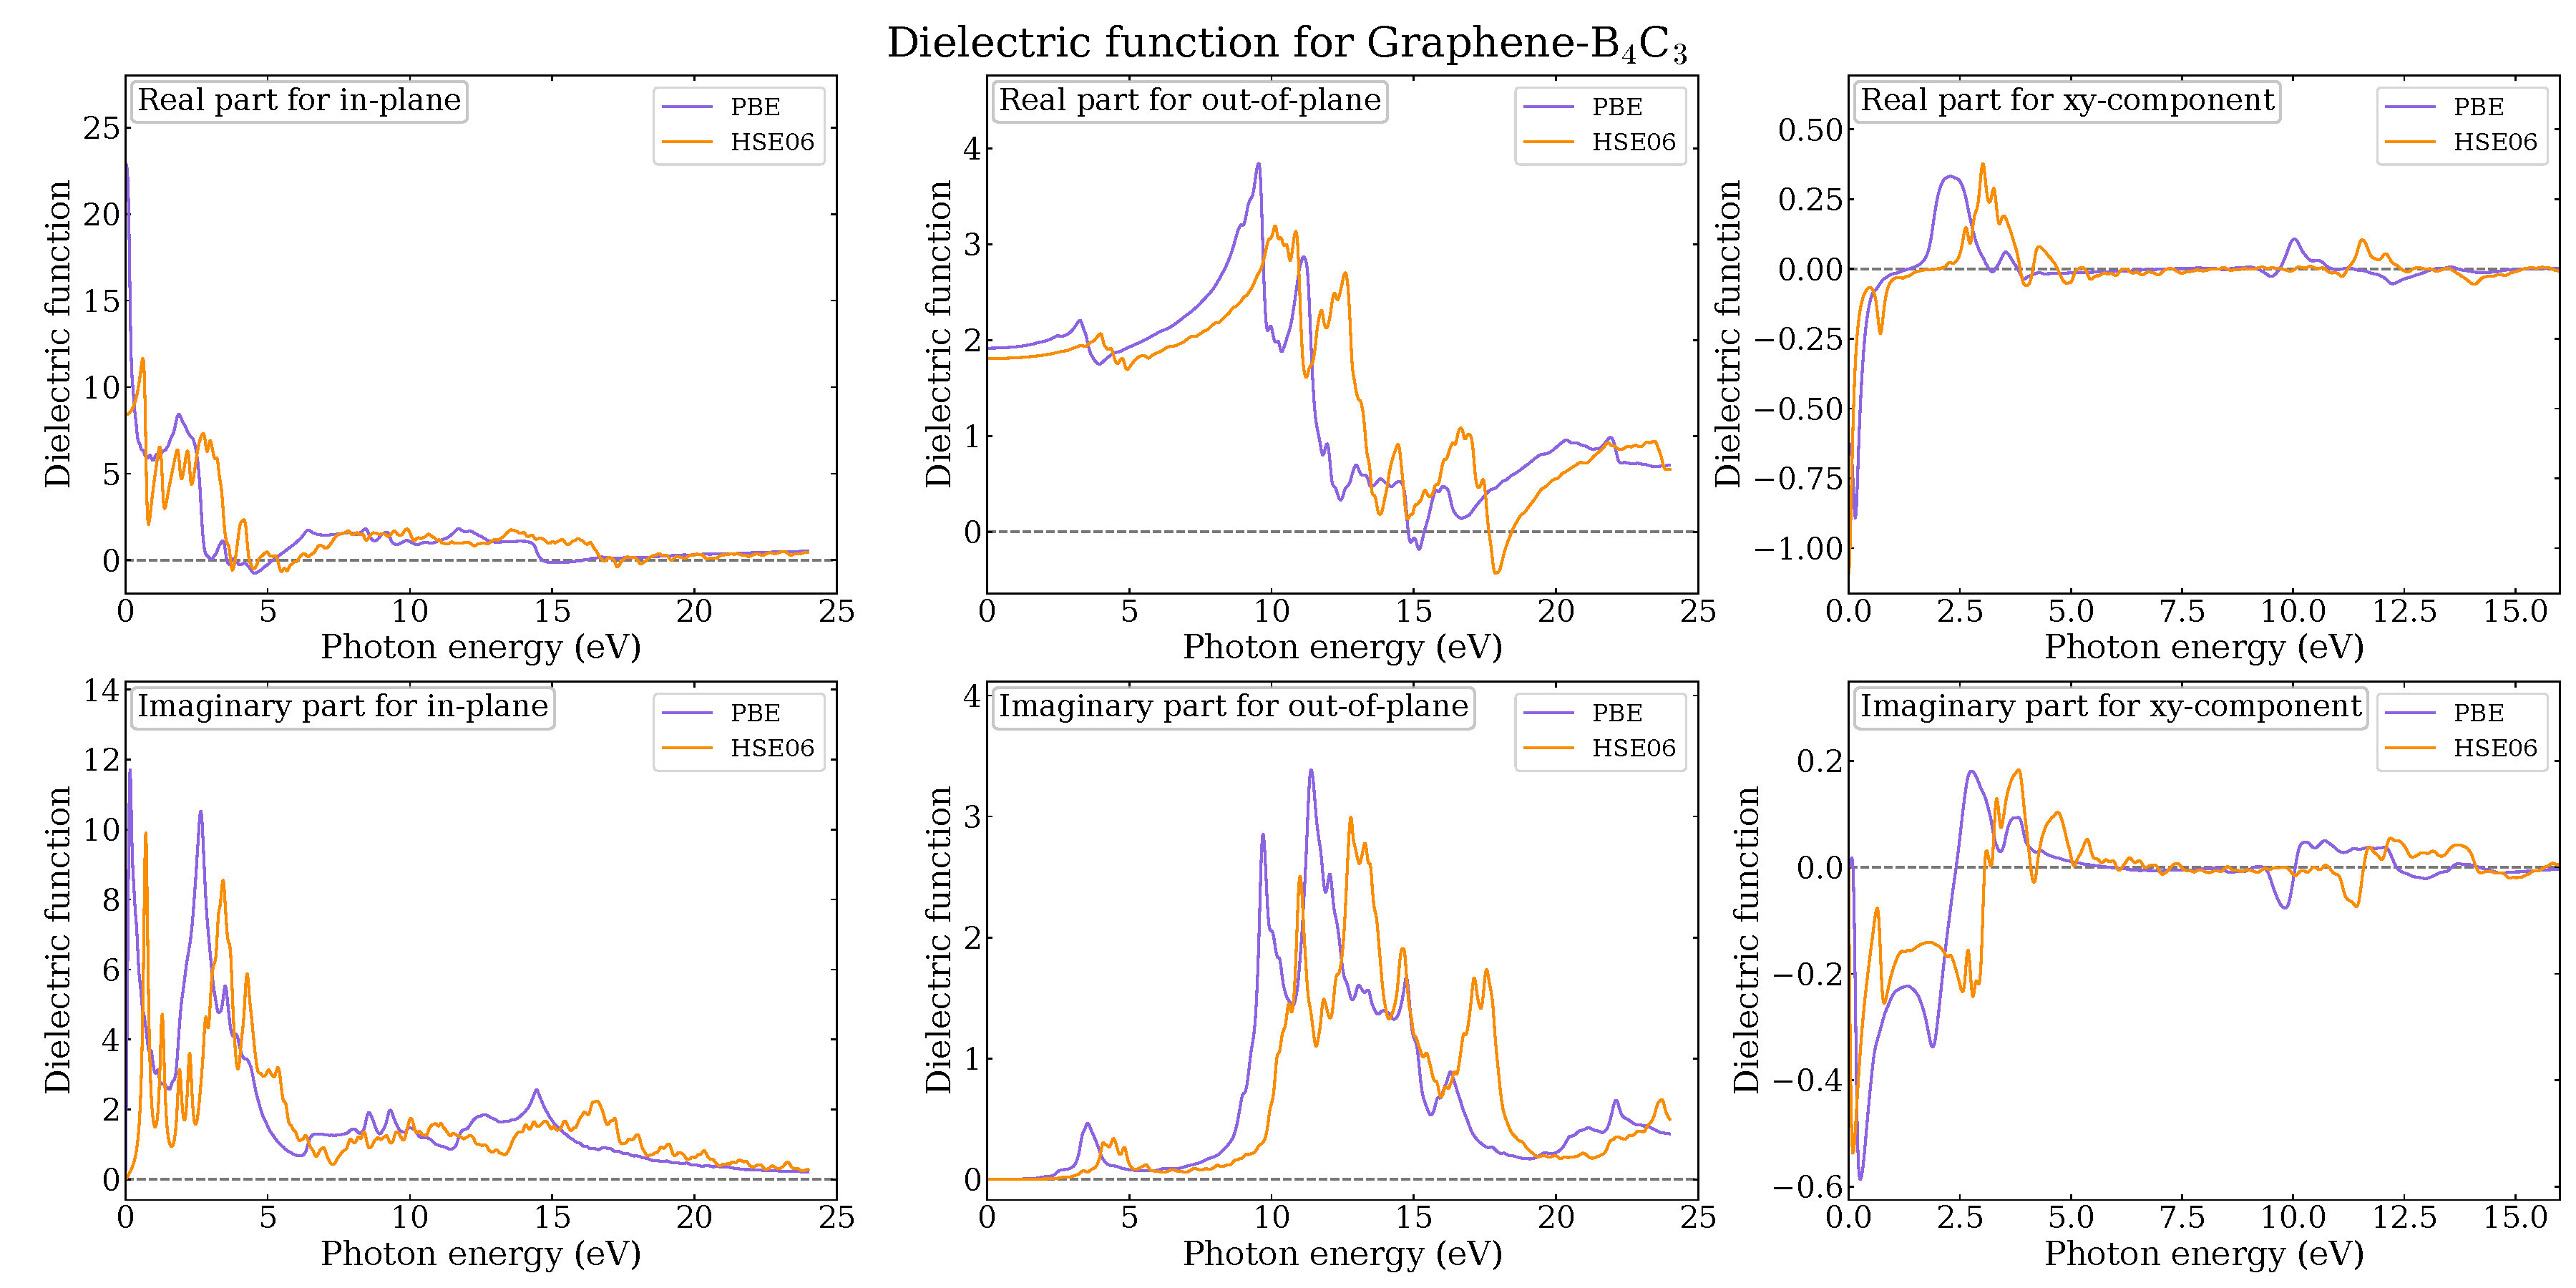
\includegraphics[width=1.00\textwidth]{figures_proj1/proj1.11_diff.pdf}
\caption{In-plane, out-of-plane, and off-diagonal $\varepsilon_{xy}$ components of the dielectric function for the Graphene-\ce{B4C3} heterostructure.}
\label{fig1.11}
\end{figure}

\subsection{Derived optical properties}

To further examine the optical properties of the heterostructure bilayers,
we calculate the absorption coefficient, energy-loss spectrum, reflectivity, refractive index, and extinction coefficient.

Figure~\ref{fig1.12} shows the HSE06 absorption coefficients and energy-loss spectra of the three systems for in-plane and out-of-plane polarizations.
The corresponding component-resolved HSE06 results are provided in figures~\ref{S1.20}--\ref{S1.24}.

The absorption threshold is determined by the onset of optically allowed transitions
and can differ from the first maximum of $\varepsilon_2(\omega)$.
For all systems, the absorption coefficient starts from a very small value and increases with photon energy,
consistent with the lowest direct transition energies in the band structure.
All three systems absorb in the visible region, \qtyrange{1.7}{3.3}{\electronvolt}.
Around \qty{1}{\electronvolt}, the Graphene-Borophene heterostructure shows a sharp rise
and a larger absorption coefficient than the other two systems.
This feature can be attributed to transitions between the flat valence-band region around the $\Gamma$ point and the low-lying conduction band in the same region of the Brillouin zone.
The Graphene-\ce{BC3} heterostructure shows a similar sharp rise at a slightly higher energy, around \qty{2.5}{\electronvolt},
followed by Graphene-\ce{B4C3} at around \qty{3.5}{\electronvolt}.
These latter features arise from transitions between relatively flat valence and conduction bands along the $\Gamma$--$\mathrm{M}$ direction.

\begin{figure}[!htbp]
\centering
    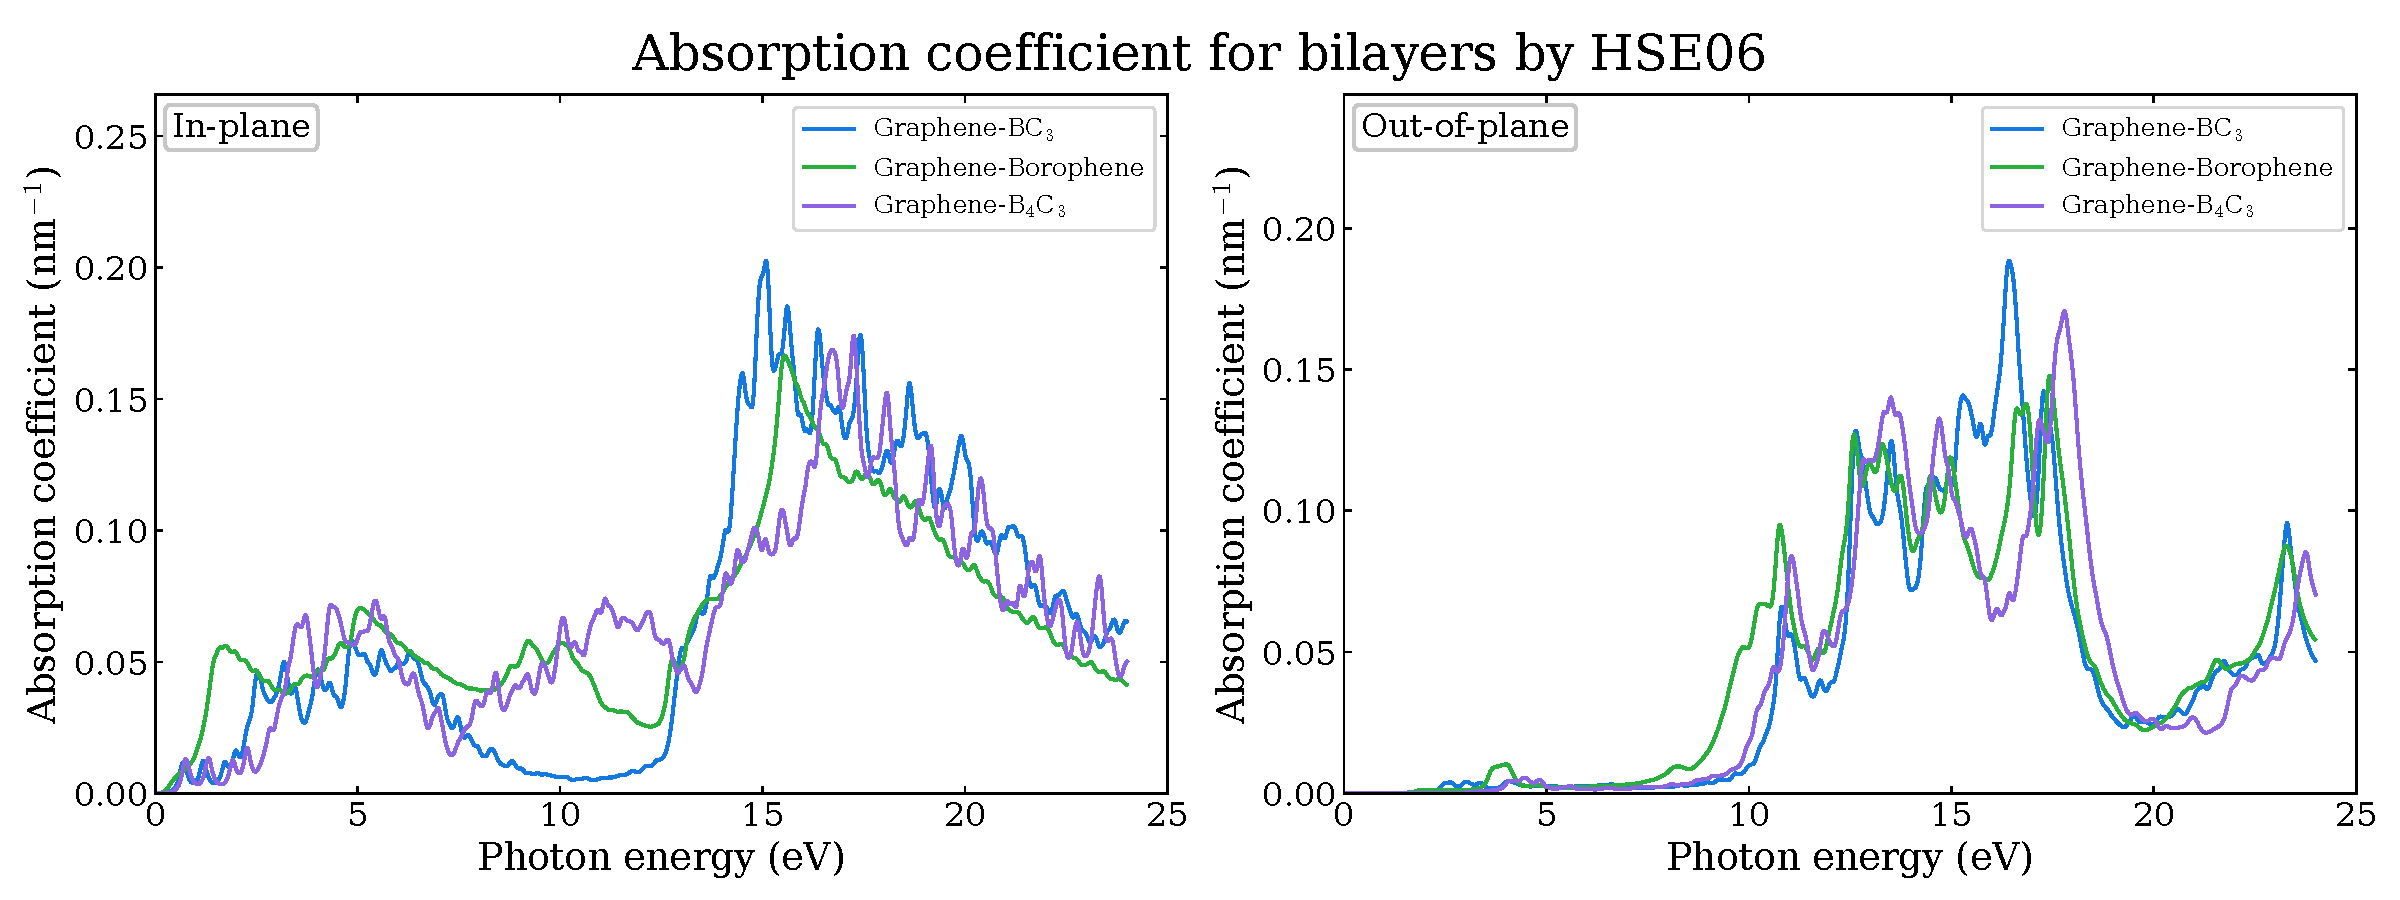
\includegraphics[width=0.80\textwidth]{figures_proj1/proj1.12a.pdf}
    \par\nointerlineskip
    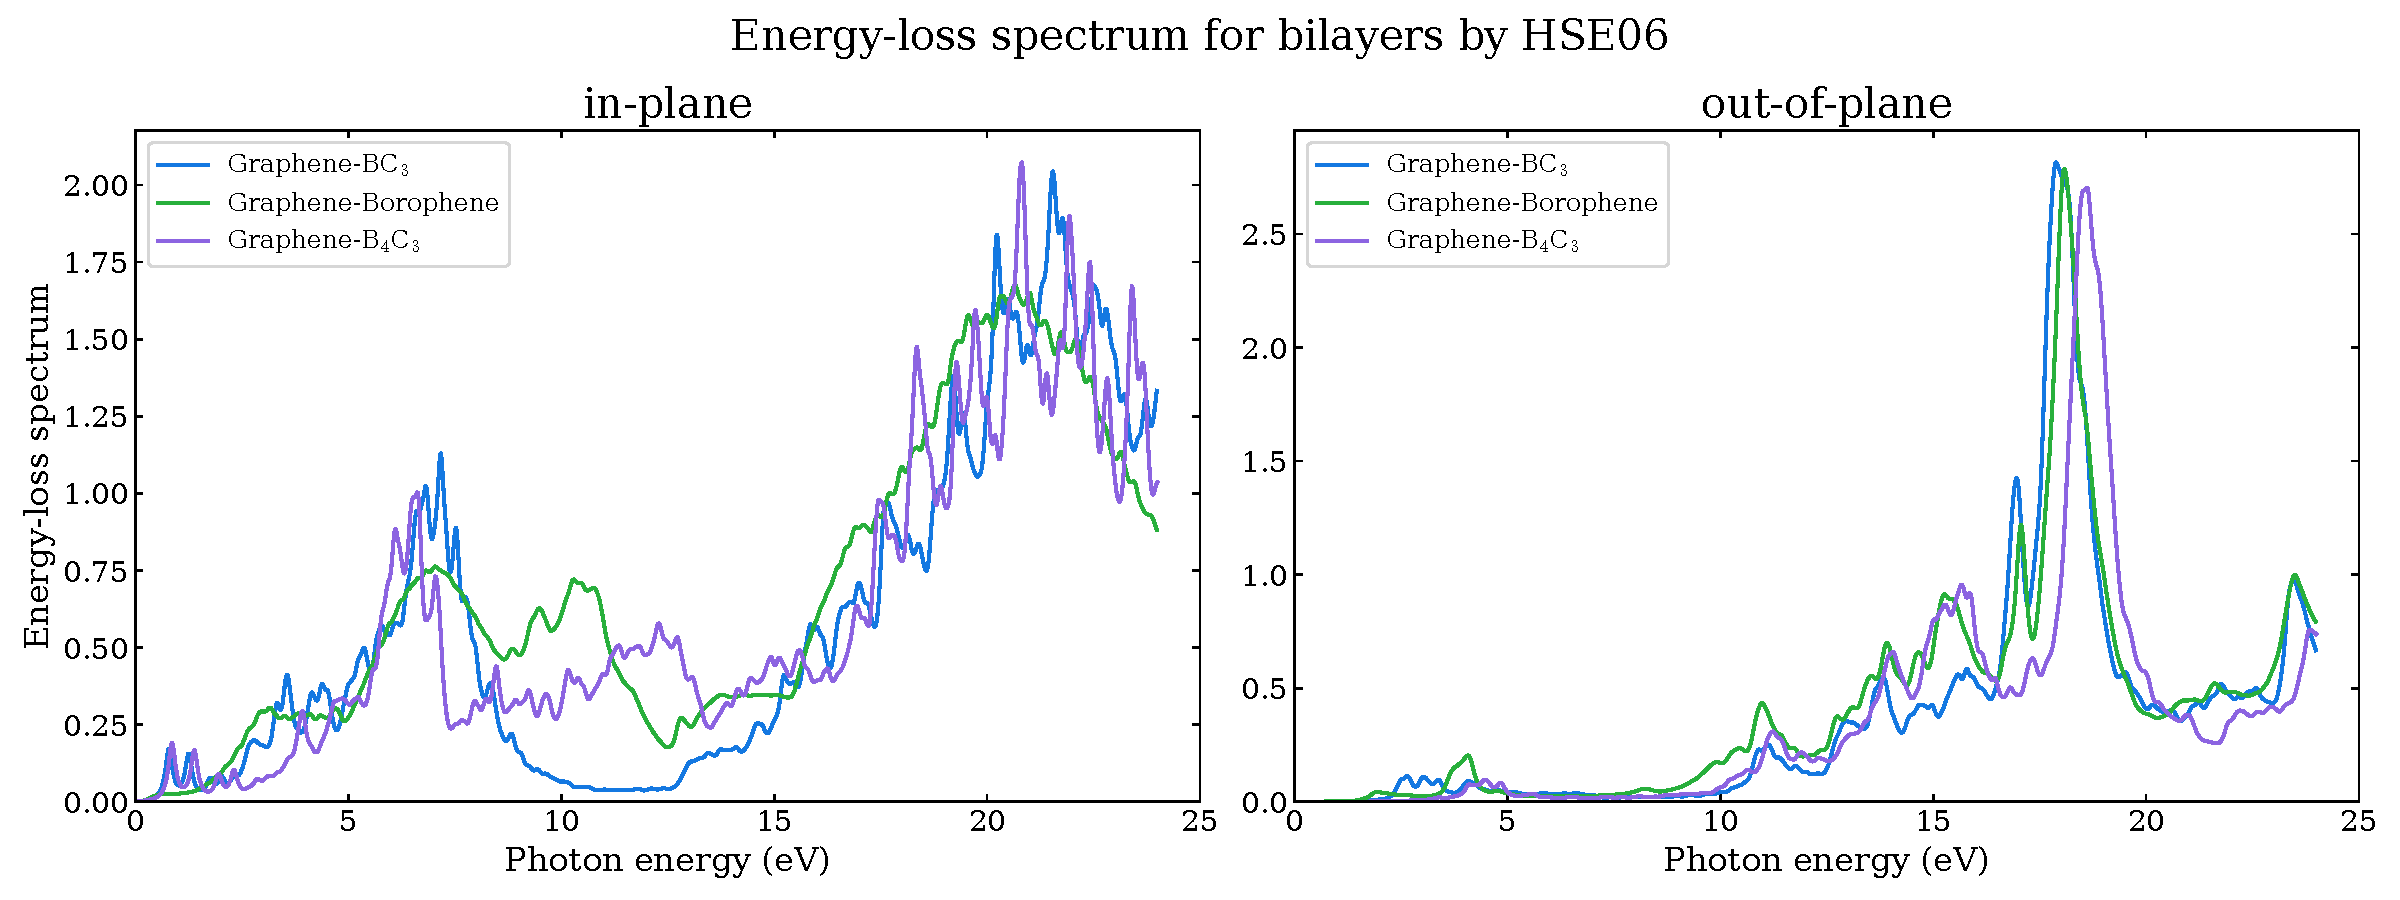
\includegraphics[width=0.80\textwidth]{figures_proj1/proj1.12b.pdf}
\caption{In-plane and out-of-plane HSE06 absorption coefficients in \si{\per\nano\metre} (upper panels)
and dimensionless energy-loss spectra (lower panels) of the three heterostructure bilayers.}
\label{fig1.12}
\end{figure}

The energy-loss spectrum in figure~\ref{fig1.12} shows a sharp in-plane loss feature below \qty{1}{\electronvolt} for Graphene-\ce{BC3} and Graphene-\ce{B4C3},
which is absent for Graphene-Borophene.
This feature may be related to Dirac-like plasmons.
The broader features between \qtyrange{3}{8}{\electronvolt} may be associated with $\pi$-like plasmons.
Individual interband transitions presumably coexist with these plasmons and form a broad background.
When interband transitions and plasmons occur in the same energy range,
the two types of excitations can couple,
giving finite plasmon lifetimes as well as interband-transition character.
The features around \qty{15}{\electronvolt}, where a sharp increase begins, may be associated with $\pi-\sigma$-type plasmons.
This assignment is consistent with the negative real part of the out-of-plane dielectric-function component,
which is one of the conditions for a plasmon resonance.

Figure~\ref{fig1.13} shows the reflectivity and refractive index of the three heterostructures,
as obtained using the HSE06 functional for in-plane and out-of-plane polarizations.
The refractive index is related to the real and imaginary parts of the dielectric function.
Its trend is similar to that of $\varepsilon_1$,
indicating that the real part of the dielectric function plays the leading role.
The refractive index determines how much the path of light is bent, or refracted, when light enters a material.
For visible light, most transparent materials have refractive indices between 1 and 2.
The absolute refractive index of an optical medium is defined as the ratio between the speed of light in vacuum and the phase velocity of light in the material,
where the phase velocity is the speed at which the crests of the light wave propagate.
Therefore, if the phase velocity is larger than the speed of light in vacuum,
the refractive index can be smaller than 1.
For frequencies near the plasmon resonance in 2D materials,
the refractive index can drop below 1 due to the strong interaction between light and plasmonic oscillations.

\begin{figure}[!htbp]
\centering
    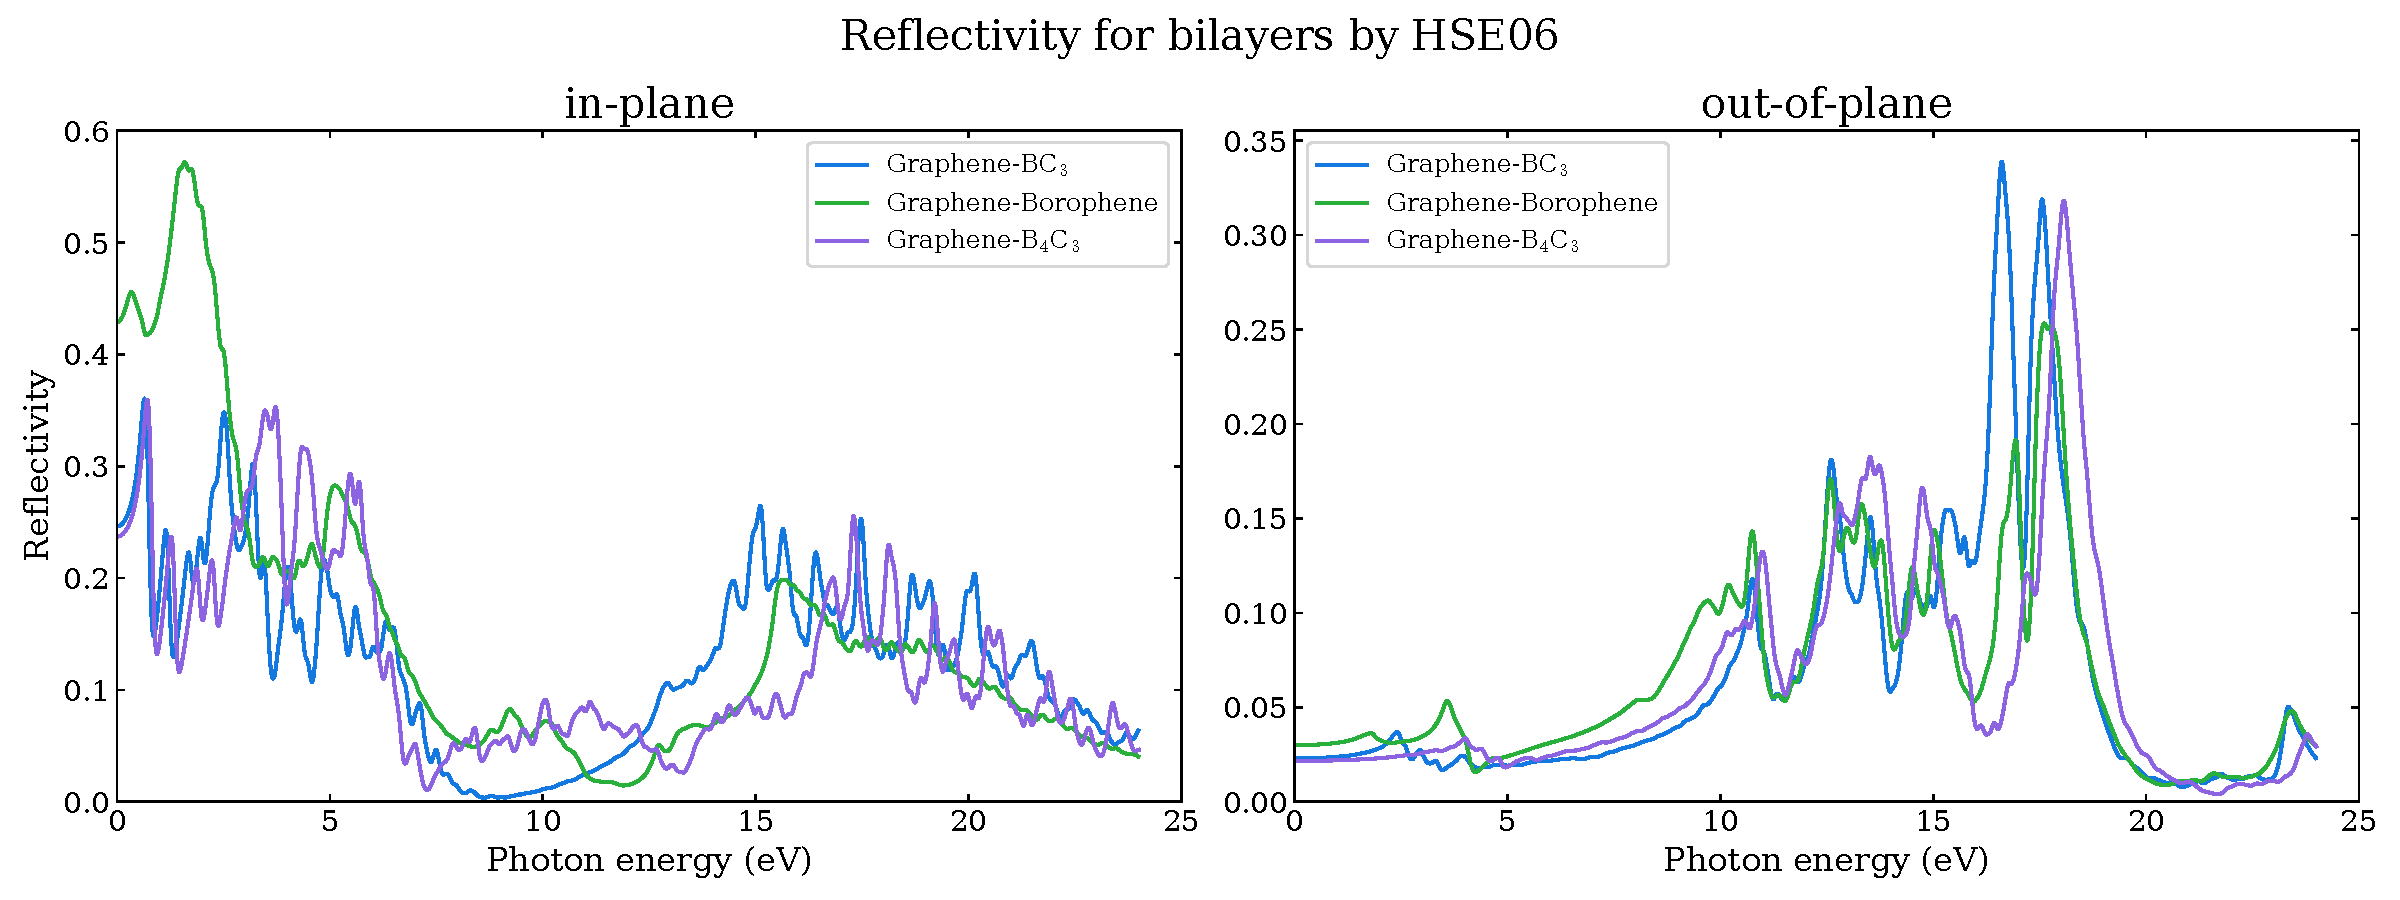
\includegraphics[width=0.80\textwidth]{figures_proj1/proj1.13a_cor.pdf}
    \par\nointerlineskip
    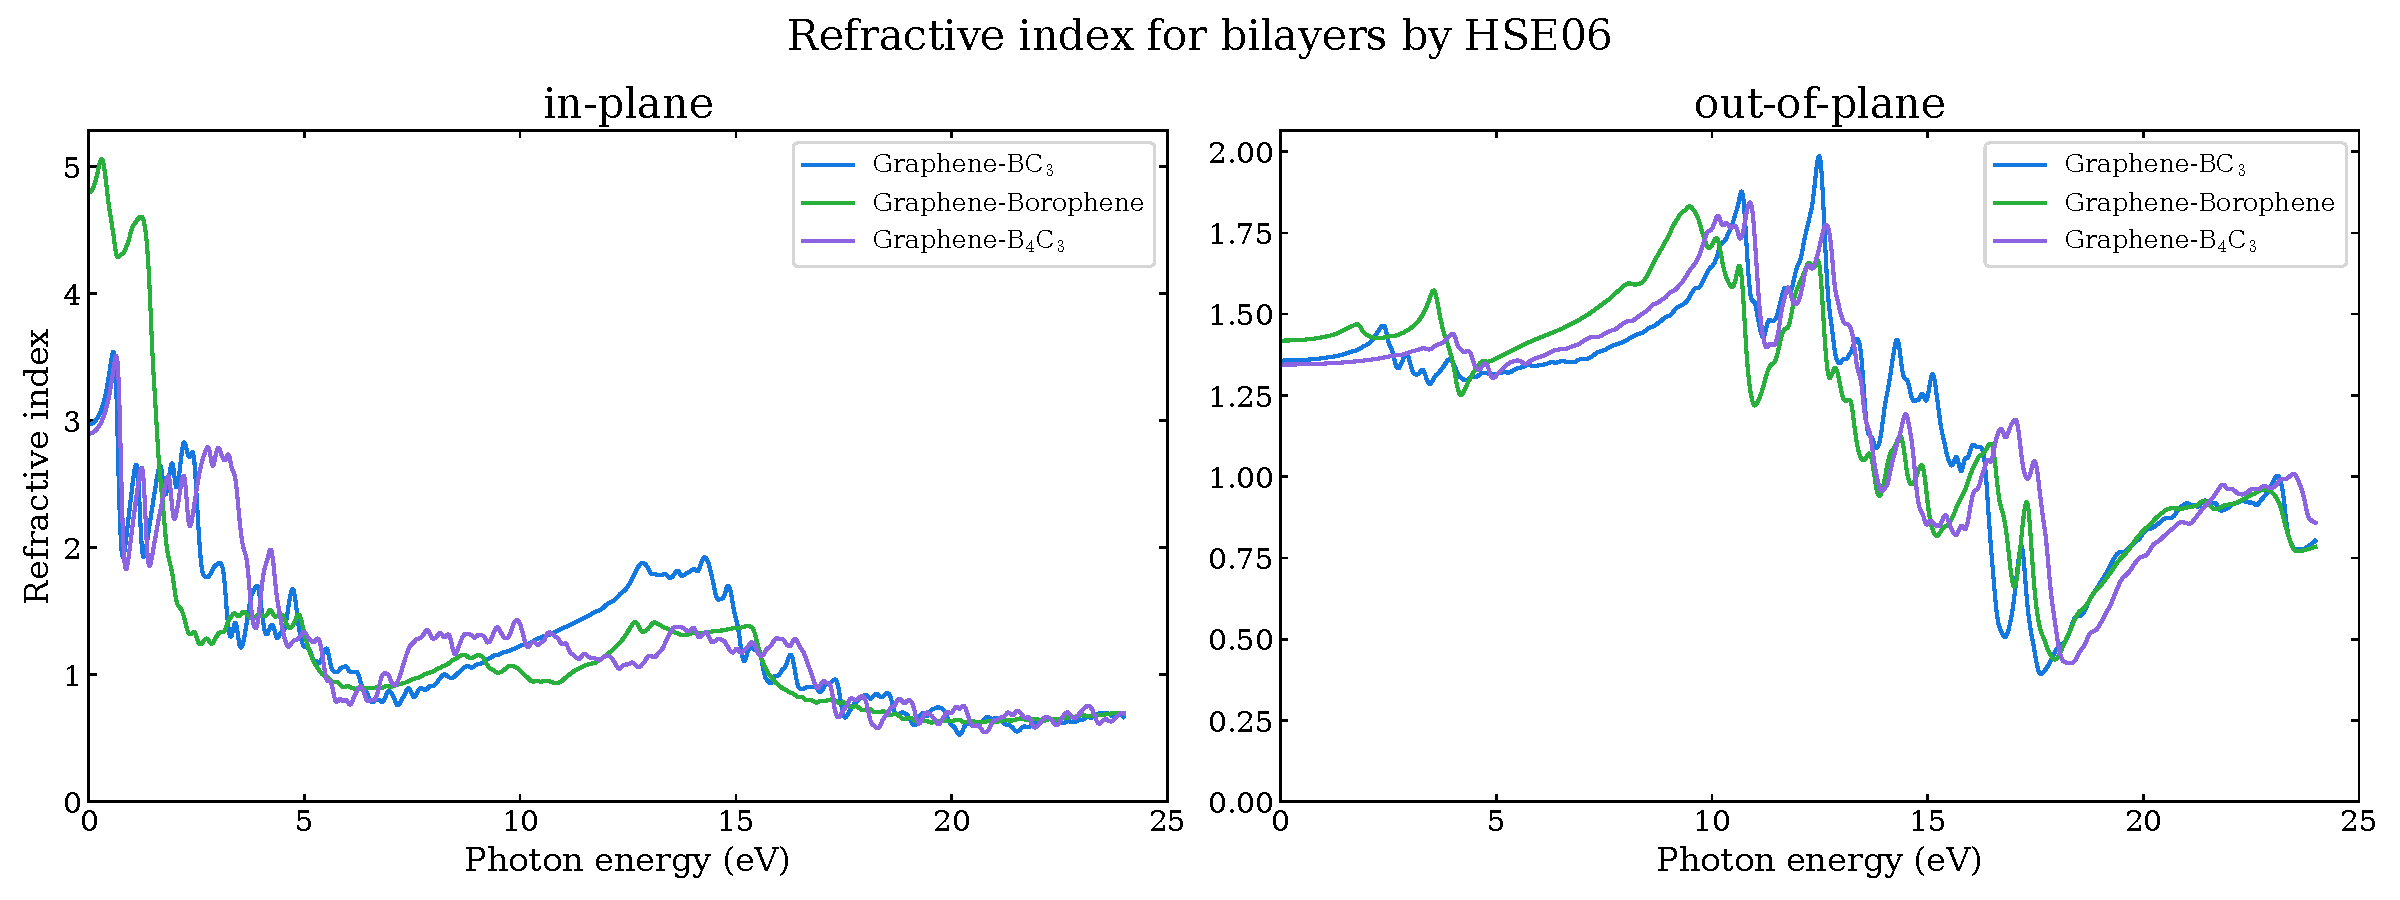
\includegraphics[width=0.80\textwidth]{figures_proj1/proj1.13b.pdf}
\caption{In-plane and out-of-plane reflectivity and refractive index of the three heterostructure bilayers.}
\label{fig1.13}
\end{figure}

The reflectivity spectra also show a clear polarization dependence.
For in-plane polarization, Graphene-Borophene exhibits the strongest response below approximately \qty{5}{\electronvolt}, while Graphene-\ce{BC3} and Graphene-\ce{B4C3} show oscillatory but weaker reflection in the same range.
All three systems then enter a low-reflectivity region from approximately \qtyrange{7}{13}{\electronvolt}.
Above this range, Graphene-\ce{BC3} and Graphene-\ce{B4C3} recover weak oscillatory features and gradually decay at higher photon energies, while Graphene-Borophene reaches a smaller peak around \qty{16}{\electronvolt} before also decreasing.
For out-of-plane polarization, the low-energy reflectivity remains small for all three systems, while pronounced peaks emerge around \qtyrange{16}{18}{\electronvolt}, consistent with the plasmon-related structures discussed above.

For in-plane polarization,
the refractive index is close to, or smaller than, 1 in the energy range of approximately \qtyrange{5}{7}{\electronvolt}
and above approximately \qty{17}{\electronvolt} for all three systems.
For out-of-plane polarization,
the refractive index is close to, or smaller than 1 for energies above about \qty{14}{\electronvolt}.
These low-index regions occur near plasmon-related energies and indicate a strong dispersive dielectric response.
Their optical transparency is interpreted together with the extinction coefficient and energy-loss spectrum, because attenuation can remain strong where the refractive index is close to or smaller than 1.

Figure~\ref{fig1.14} shows the HSE06 extinction coefficient for in-plane and out-of-plane polarizations.
For in-plane polarization, the strongest response occurs in the low-energy region for all three heterostructures.
Graphene-Borophene exhibits the largest peak below approximately \qty{2}{\electronvolt} and remains relatively strong up to about \qty{6}{\electronvolt}, whereas Graphene-\ce{BC3} and Graphene-\ce{B4C3} show weaker oscillatory features over approximately \qtyrange{1}{6}{\electronvolt}.
All three systems then enter a suppressed region around \qtyrange{7}{13}{\electronvolt}, where the response of Graphene-\ce{BC3} becomes particularly weak,
followed by broader secondary features in the higher-energy range.
For out-of-plane polarization, the extinction coefficient is small at low photon energies but rises strongly in the ultraviolet region, where pronounced peaks emerge mainly between approximately \qtyrange{10}{18}{\electronvolt}.
These energy regions therefore correspond to strong photon attenuation.

\begin{figure}[!htbp]
\centering
    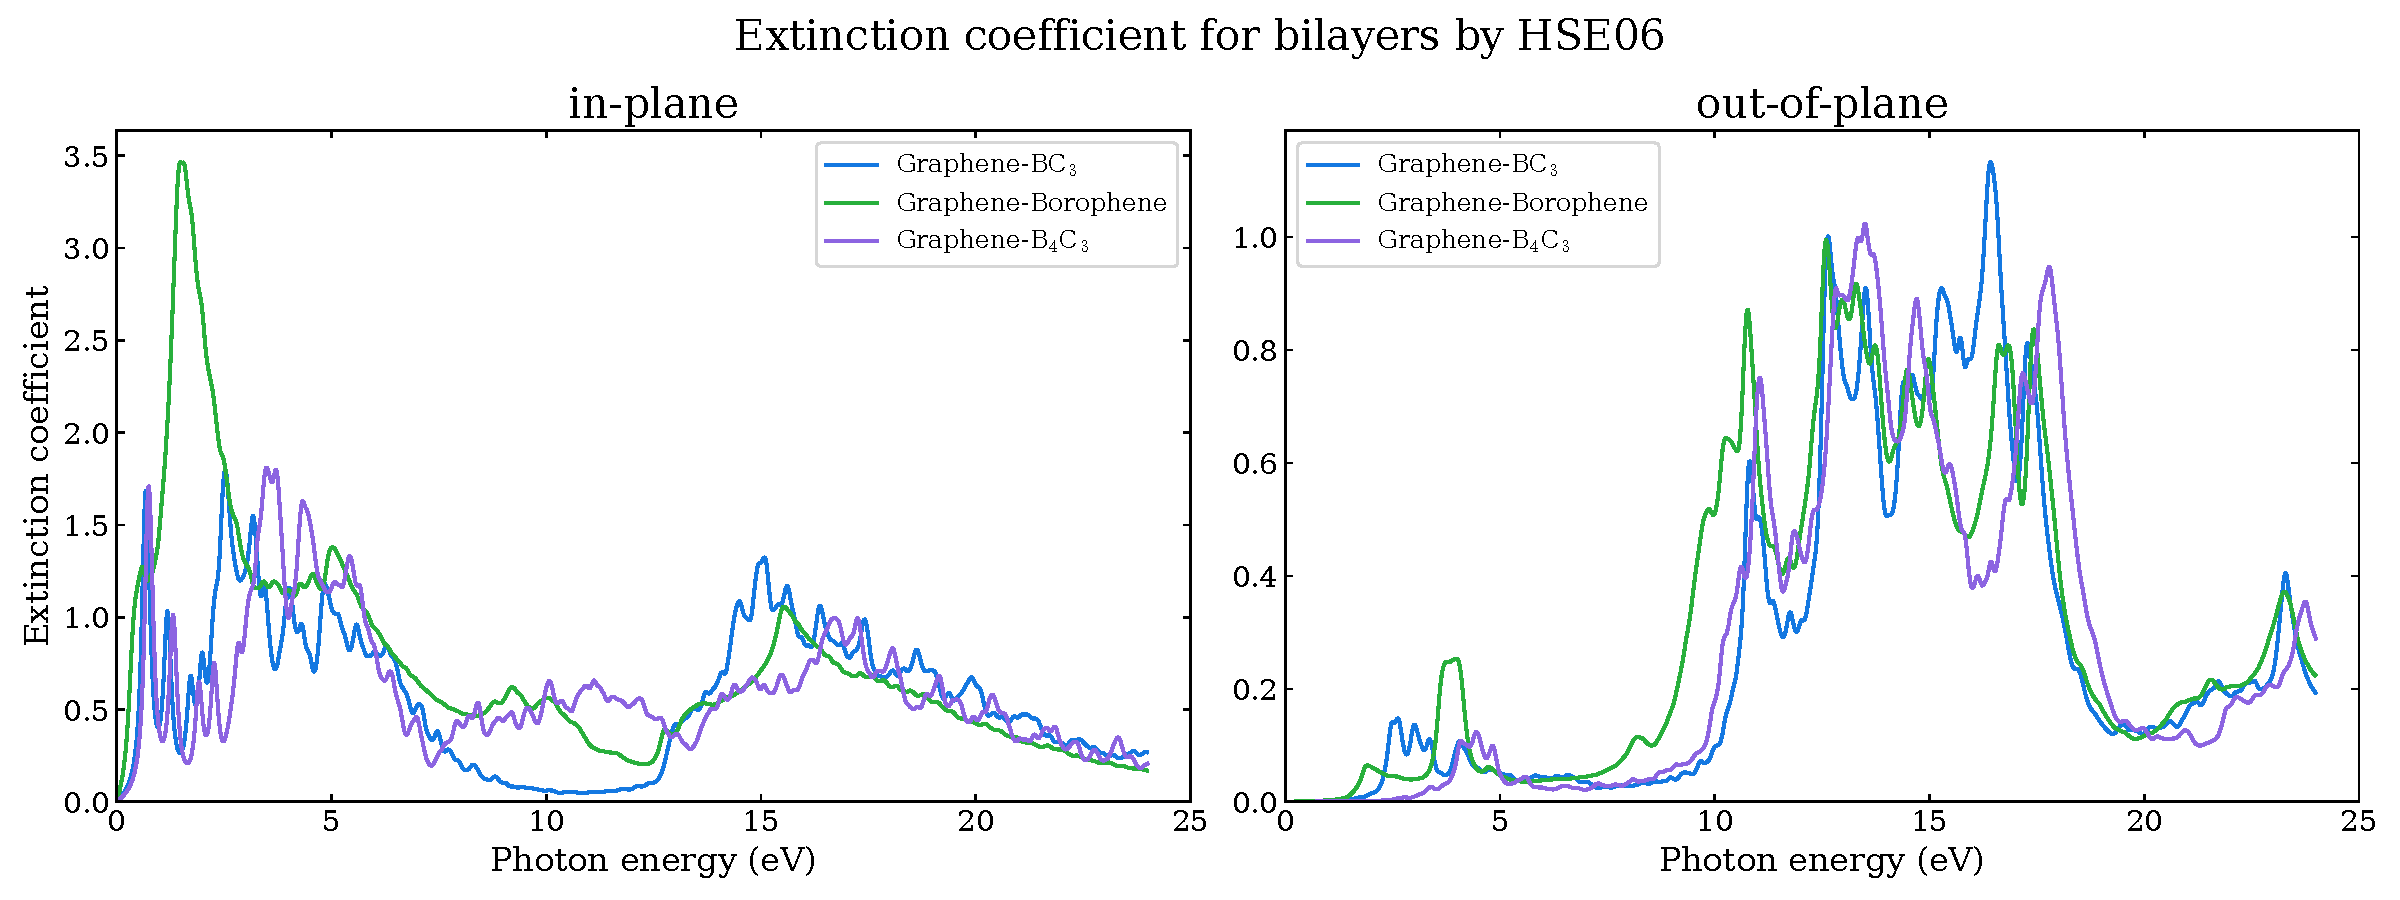
\includegraphics[width=0.80\textwidth]{figures_proj1/proj1.14_cor.pdf}
\caption{In-plane and out-of-plane extinction coefficients of the three heterostructure bilayers.}
\label{fig1.14}
\end{figure}

\section{Conclusions}
\label{1_conclusions}

In the present work,
we investigated the atomic, electronic, and optical properties of Graphene-Borophene,
Graphene-\ce{BC3}, and Graphene-\ce{B4C3} bilayer heterostructure systems
using first-principles calculations with the HSE06 and PBE functionals.
We find that all systems have small binding energies between the layers,
indicating that graphene interacts weakly with the monolayers through van der Waals interactions.
The Graphene-Borophene bilayer is metallic,
whereas the Graphene-\ce{BC3} and Graphene-\ce{B4C3} structures maintain the characteristic linear bands of graphene around the $\mathrm{K}$ point,
with only a very small band-gap opening of \qtyrange{20}{50}{\milli\electronvolt}.
The calculated optical properties show absorption in the visible region of the spectrum for all heterostructures,
with Graphene-Borophene showing the strongest response near its low-energy absorption onset.
All heterostructures show features consistent with plasmon resonances in the calculated dielectric and energy-loss spectra.
For Graphene-Borophene,
the in-plane real dielectric function has low-energy negative regions around \qty{2}{\electronvolt} and \qty{5}{\electronvolt}.
These intervals are distinct from the sub-eV energy-loss peaks of the other two heterostructures.
The symmetric dielectric tensor of Graphene-\ce{B4C3} follows the threefold rotational symmetry of the structure.

\clearpage
\section{Data availability statement}

The original data presented in this chapter are openly available from the \texttt{GitHub} repository:
\href{https://github.com/Photonico/Graphene-BC_20230622}{\texttt{Photonico/Graphene-BC\_20230622}}.

\section{Supplementary information}
\label{1_supplementary}

The supplementary information presents the lattice-parameter determination for the graphene, borophene, \ce{BC3}, and \ce{B4C3} monolayers,
as well as the corresponding results for the associated heterostructure bilayers under various relative lateral displacements.
It also provides k-point mesh convergence tests, projected densities of states, dielectric-function convergence tests, and derived optical properties for the monolayer and bilayer systems investigated.

\begin{figure}[!htbp]
\centering
    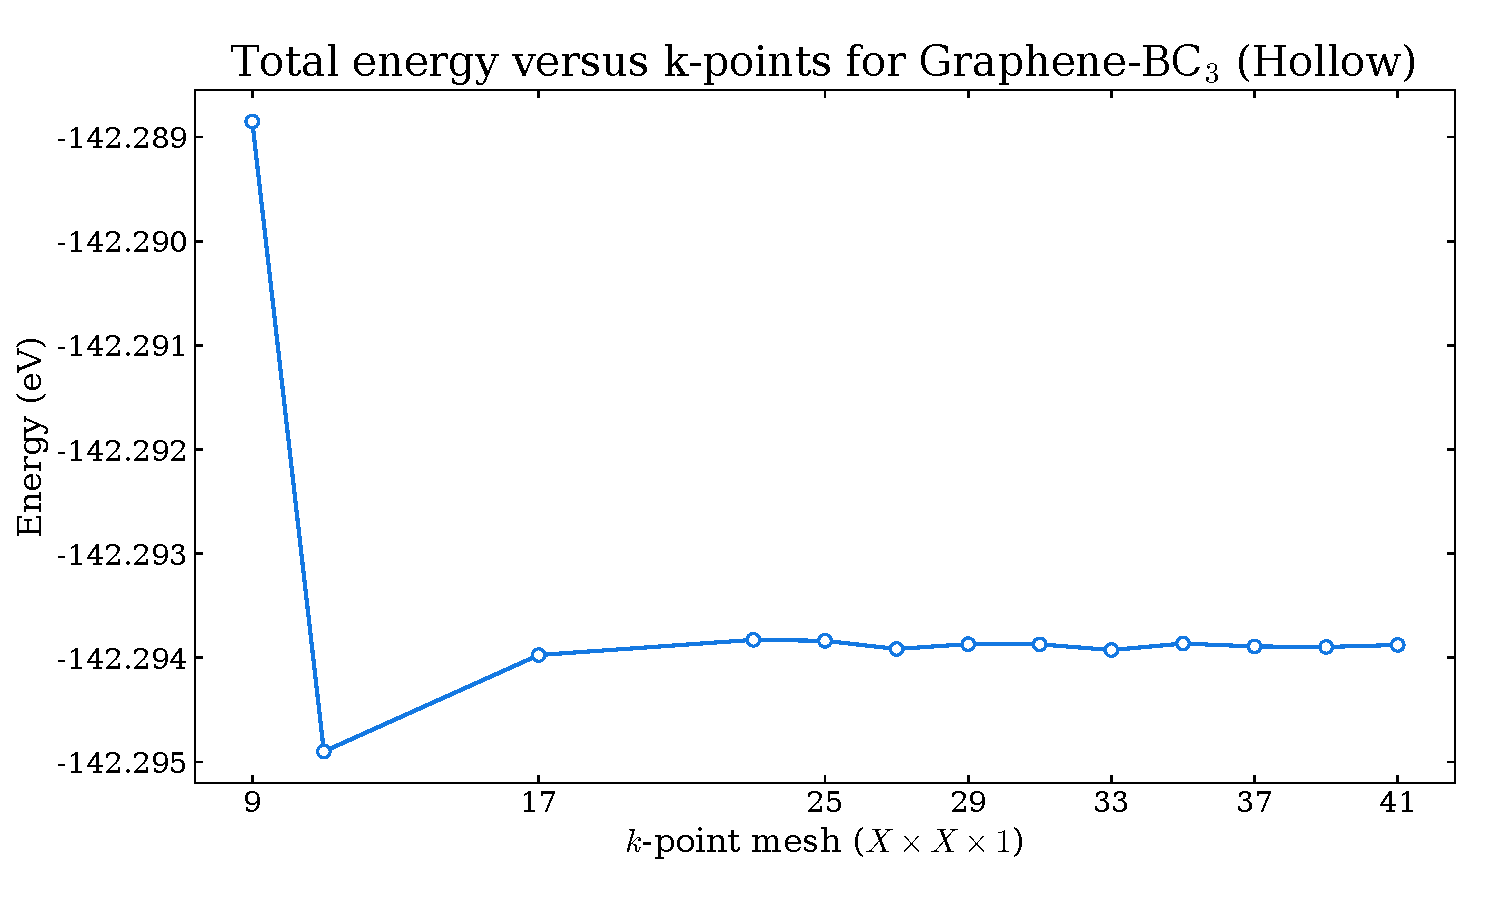
\includegraphics[width=0.60\textwidth]{figures_proj1/S1.1.pdf}
    \caption{Total energy versus the k-point mesh used to sample the Brillouin zone for the Graphene-\ce{BC3} bilayer; here, $\mathrm{X}$ denotes an $\mathrm{X} \times \mathrm{X} \times 1$~k-point mesh.}
\label{S1.1}
\end{figure}

\begin{figure}[!htbp]
\centering
    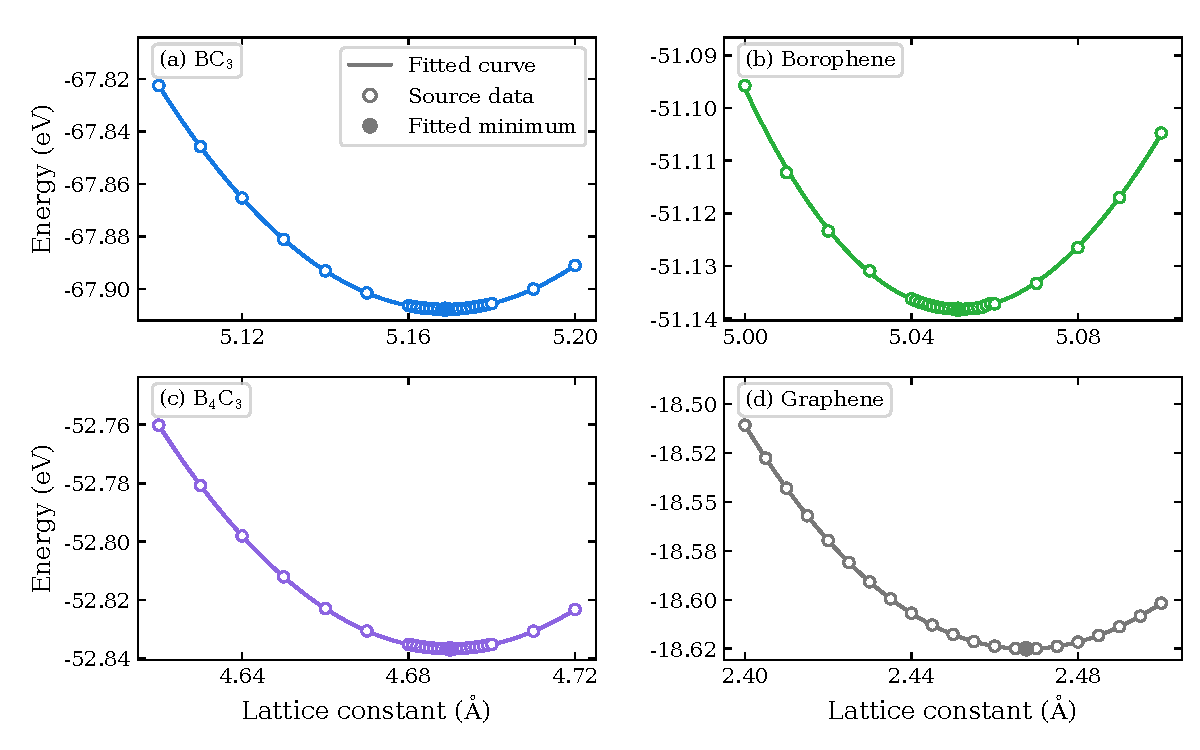
\includegraphics[width=0.80\textwidth]{figures_proj1/S1.2.pdf}
\caption{Total energy versus lattice constant for (a) \ce{BC3}, (b) borophene, (c) \ce{B4C3}, and (d) graphene.
The lattice constant yielding the lowest total energy is shown by the full circle in each plot.}
\label{S1.2}
\end{figure}

\begin{figure}[!htbp]
\centering
    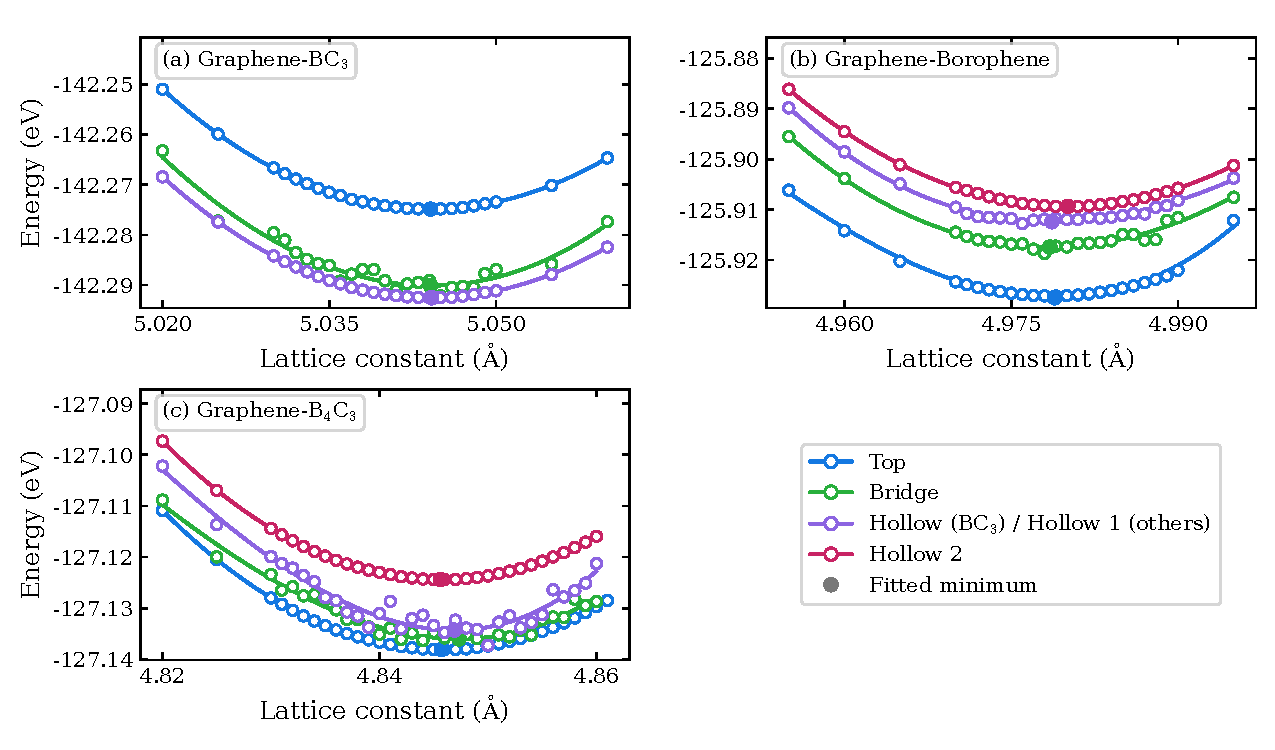
\includegraphics[width=0.80\textwidth]{figures_proj1/S1.3.pdf}
\caption{Total energy versus lattice constant for each bilayer system for the various stacking positions considered.
The lines are fitted curves, with the full circle indicating the lowest-energy structure.}
\label{S1.3}
\end{figure}

Figures~\ref{S1.4}--\ref{S1.6} show the total energy versus the lattice constant and interlayer distance for the various lateral positions considered.
The horizontal and vertical axes give the lattice constant and interlayer spacing, respectively, both in \si{\angstrom}; the colour scale gives the total energy in \unit{\electronvolt}.
The marker in each panel identifies the lowest-energy sampled geometry; the colour field interpolates the sampled energies.
These sampled minima are distinct from the relaxed structural parameters listed in table~\ref{tab:1.2_heterostructure}.

\begin{figure}[!htbp]
\centering
    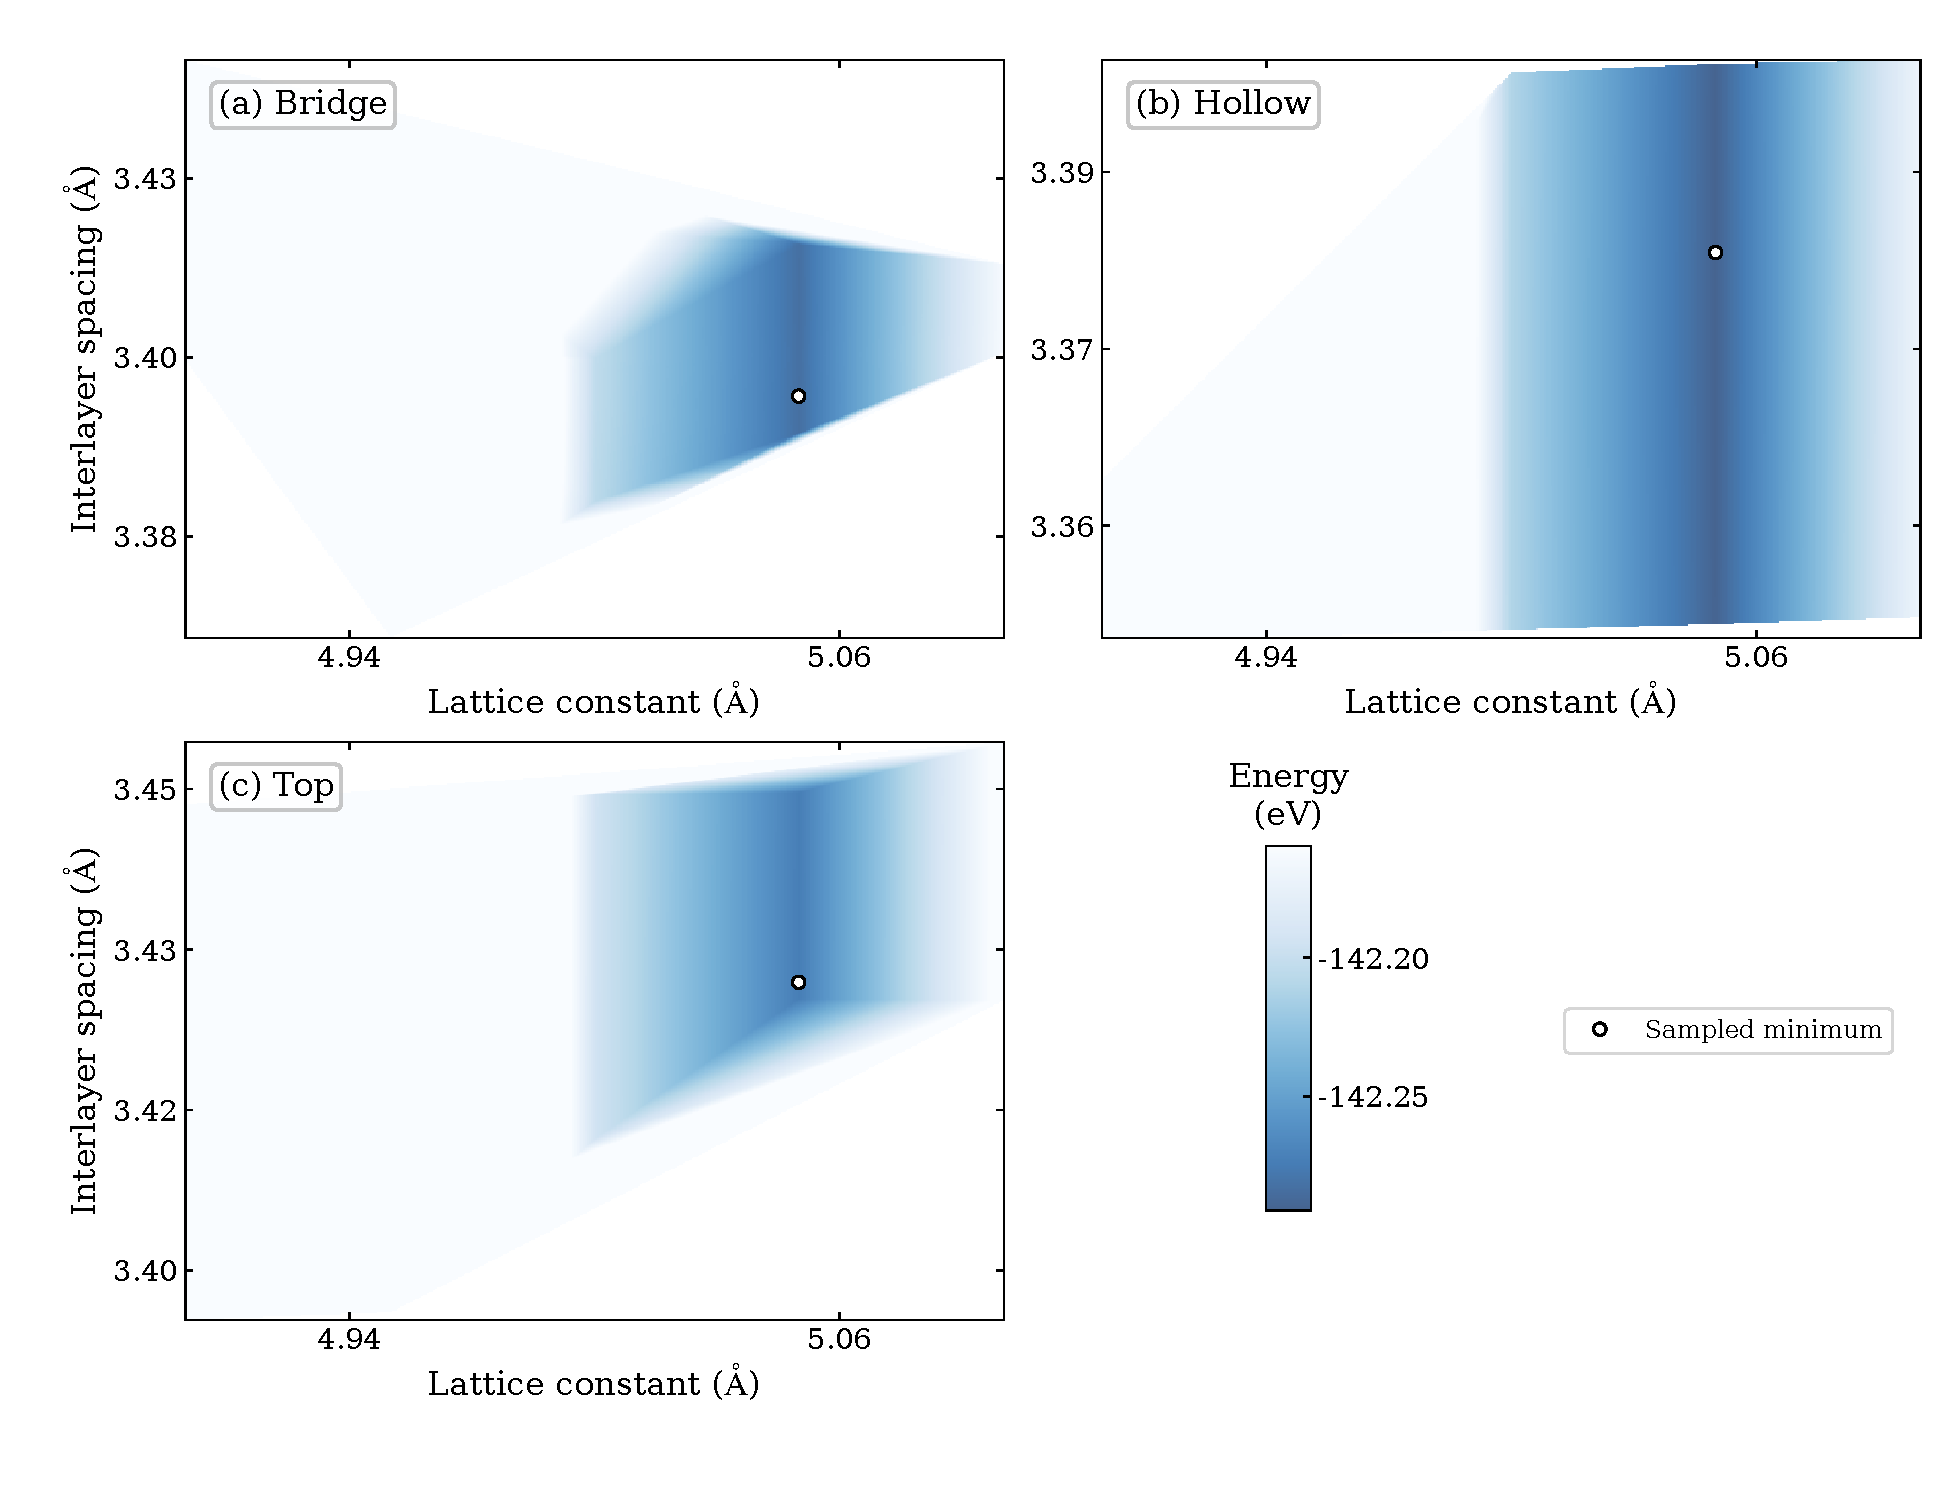
\includegraphics[width=0.80\textwidth]{figures_proj1/S1.4.pdf}
\caption{Total-energy landscape of the Graphene-\ce{BC3} bilayer.}
\label{S1.4}
\end{figure}


\begin{figure}[!htbp]
\centering
    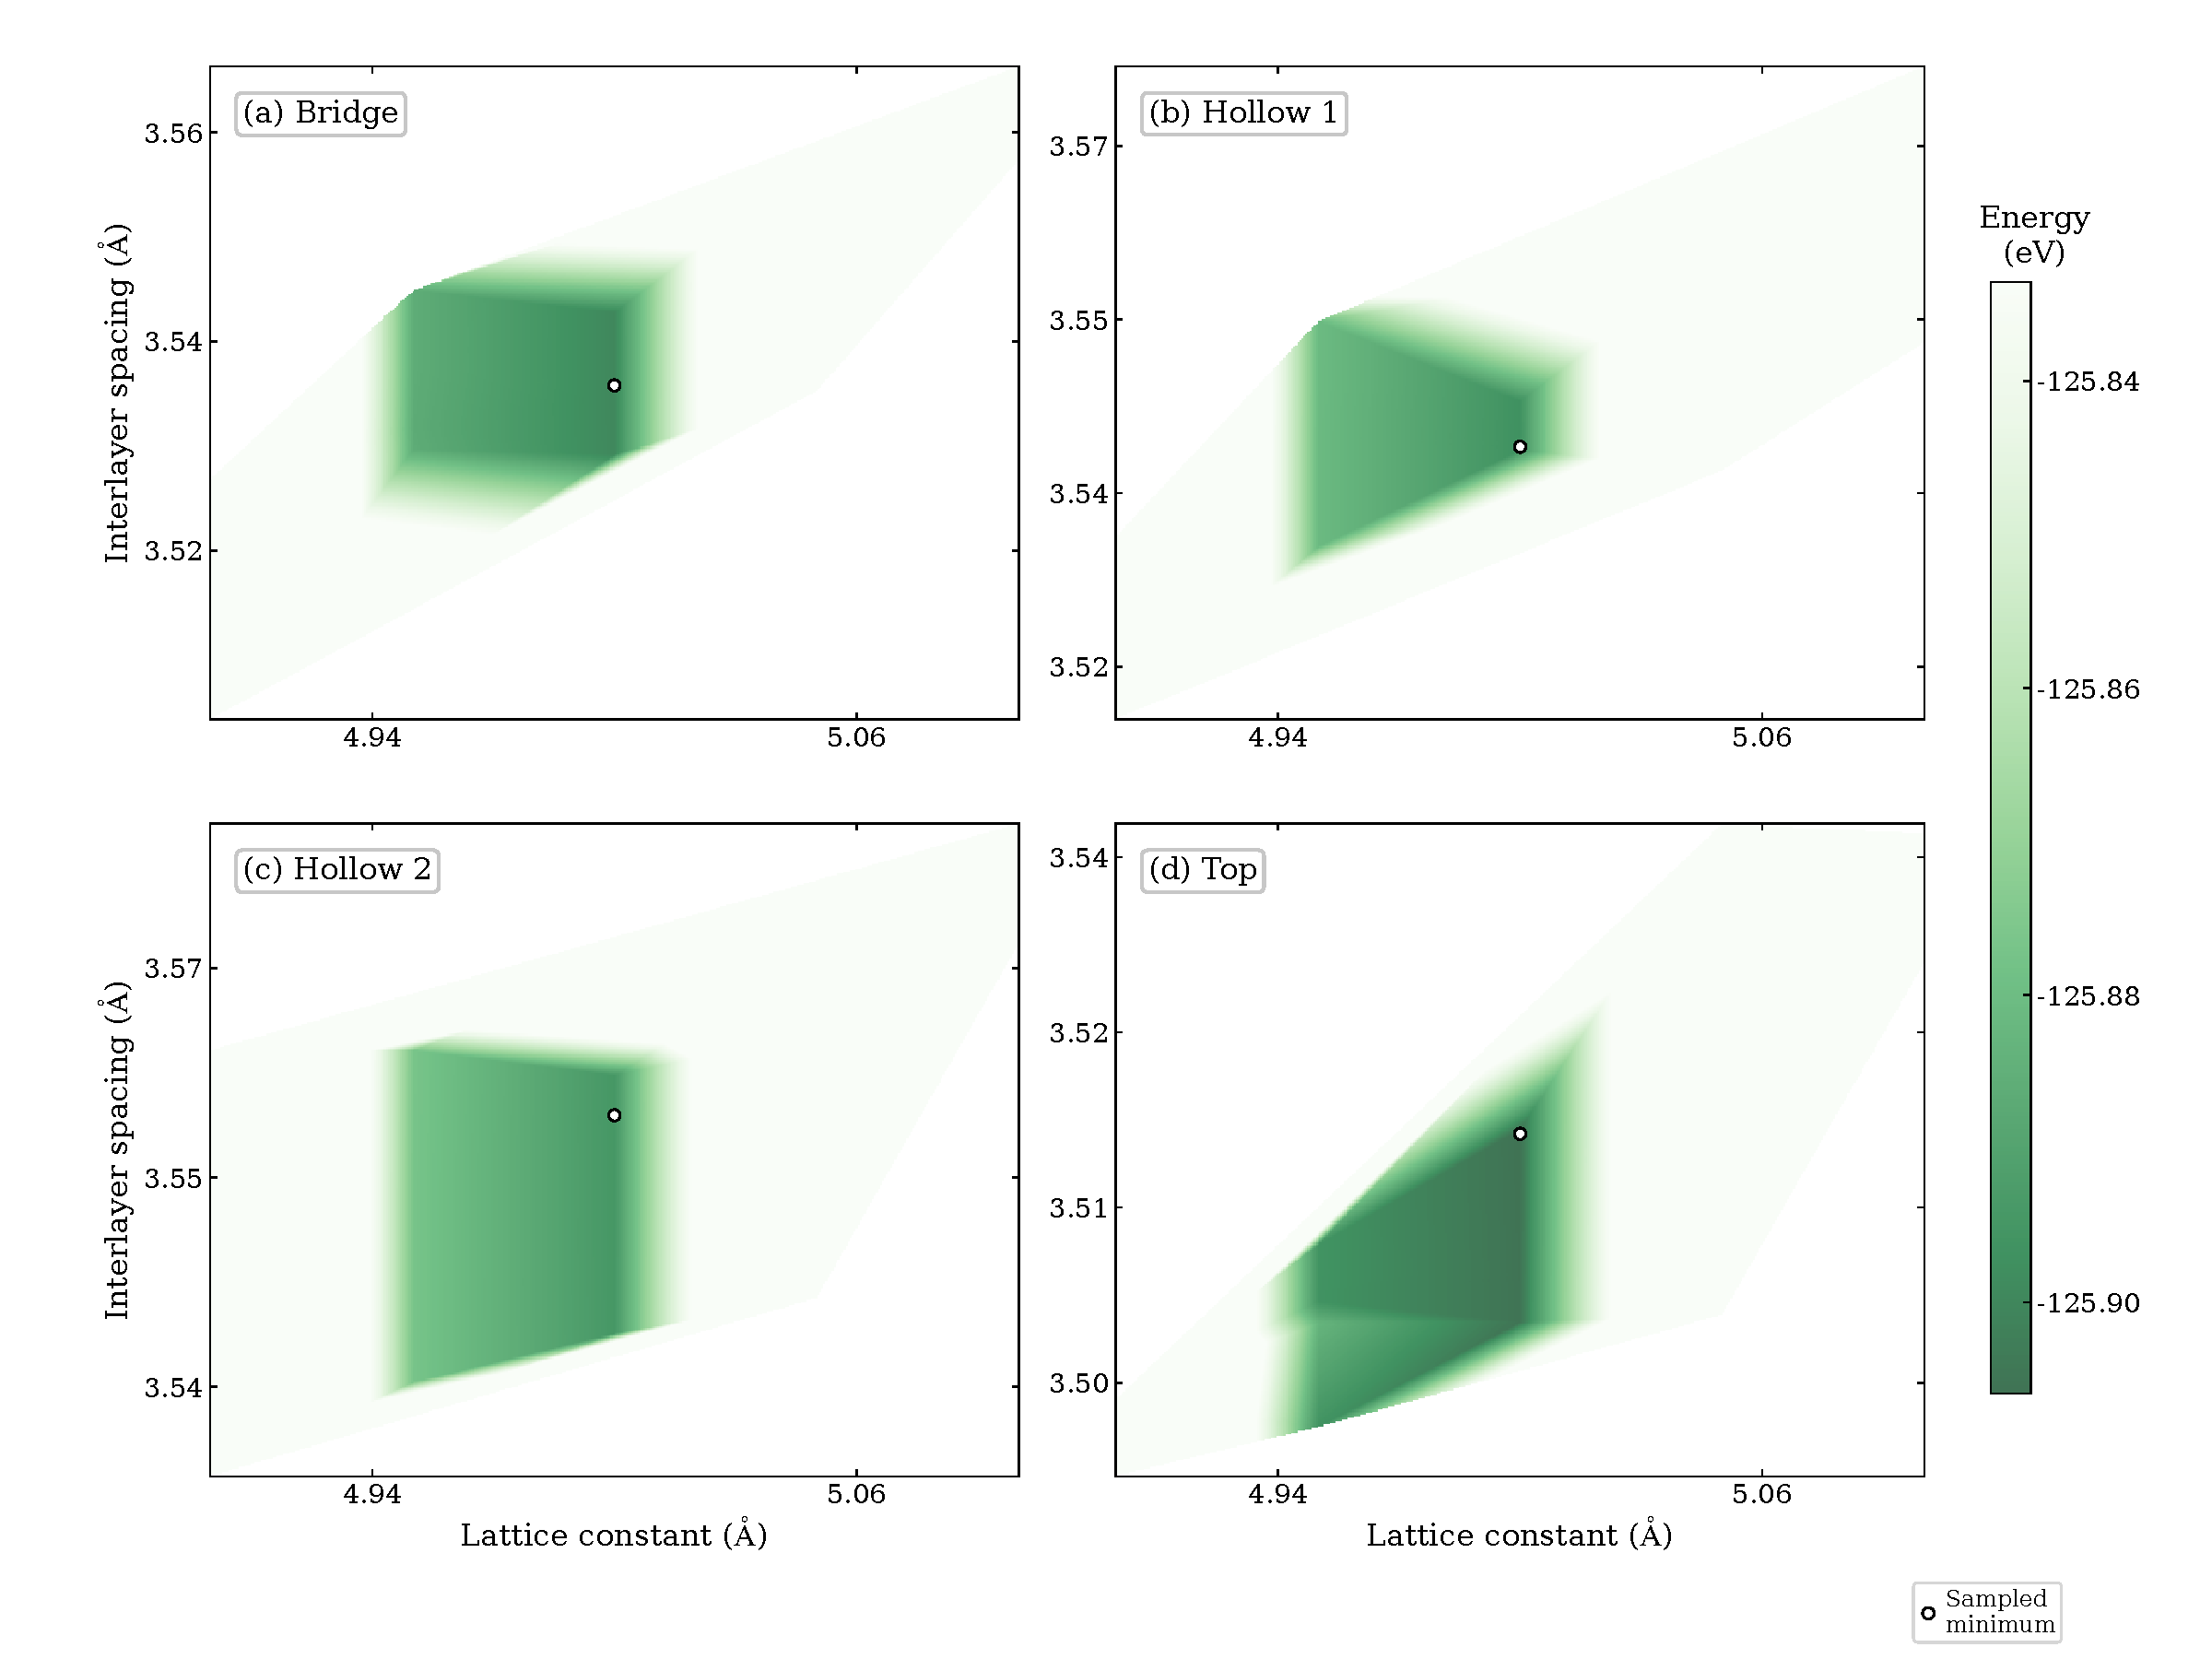
\includegraphics[width=0.80\textwidth]{figures_proj1/S1.5.pdf}
\caption{Total-energy landscape of the Graphene-Borophene bilayer.}
\label{S1.5}
\end{figure}


\begin{figure}[!htbp]
\centering
    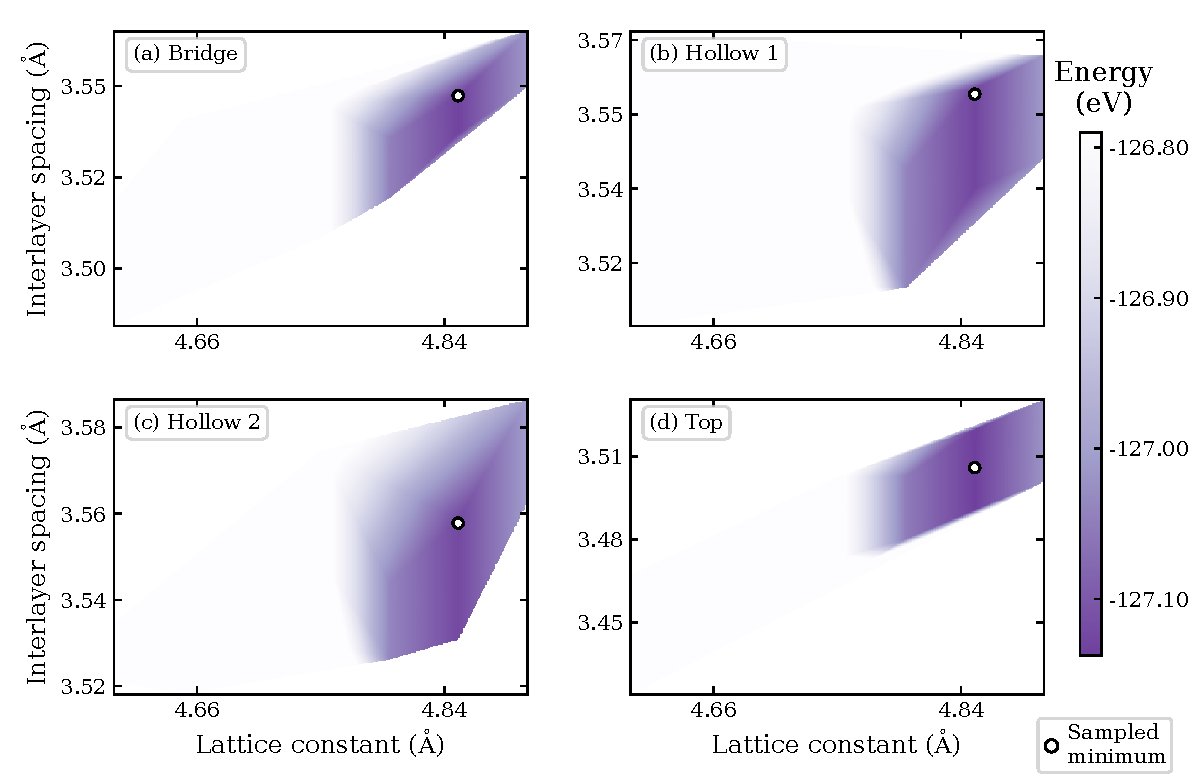
\includegraphics[width=0.80\textwidth]{figures_proj1/S1.6.pdf}
\caption{Total-energy landscape of the Graphene-\ce{B4C3} bilayer.}
\label{S1.6}
\end{figure}


\begin{table}[!htbp]
\centering
\begin{adjustbox}{max width=1.0\linewidth}
\begin{tabular}{cccccc}
\hline
\rowcolor{gray!25}
system
& site
& lattice constant (Å)
& interlayer spacing (Å)
& total energy (eV)
& relative energy (eV) \\ \hline

\multirow{3}{*}{Graphene-\ce{BC3}}
& Top
& 5.044
& 3.432
& -142.275
& 0.018 \\

& \cellcolor{gray!15} Bridge
& \cellcolor{gray!15} 5.044
& \cellcolor{gray!15} 3.384
& \cellcolor{gray!15} -142.290
& \cellcolor{gray!15} 0.002 \\

& \textbf{Hollow}
& \textbf{5.044}
& \textbf{3.375}
& \textbf{-142.293}
& \textbf{0.000} \\ \hline

\rowcolor{gray!15}
% \cellcolor{white}
\cellcolor{gray!15}
& \textbf{Top}
& \textbf{4.979}
& \textbf{3.496}
& \textbf{-125.927}
& \textbf{0.000} \\

% \cellcolor{white}
\cellcolor{gray!15}
& Bridge
& 4.979
& 3.505
& -125.921
& 0.006 \\

\rowcolor{gray!15}
% \cellcolor{white}
\cellcolor{gray!15}
& Hollow 1
& 4.979
& 3.551
& -125.914
& 0.013 \\

% \cellcolor{white}
\cellcolor{gray!15}
\multirow{-4}{*}{Graphene-Borophene}
& Hollow 2
& 4.979
& 3.548
& -125.909
& 0.018 \\ \hline

\rowcolor{gray!15}
\cellcolor{white}
& \textbf{Top}
& \textbf{4.846}
& \textbf{3.514}
& \textbf{-127.138}
& \textbf{0.000} \\

\cellcolor{white}
& Bridge
& 4.846
& 3.536
& -127.135
& 0.003 \\

\rowcolor{gray!15}
\cellcolor{white}
& Hollow 1
& 4.846
& 3.545
& -127.133
& 0.005 \\

\cellcolor{white}
\multirow{-4}{*}{Graphene-\ce{B4C3}}
& Hollow 2
& 4.846
& 3.562
& -127.124
& 0.014 \\ \hline

\end{tabular}
\end{adjustbox}
\caption{For each bilayer system and each lateral position considered, the optimized lattice constant, interlayer spacing, total energy, and relative energy are given.
The relative energy is given with respect to the most favourable structure, which corresponds to the lowest total energy for each bilayer system.}
\label{tab:S1.1}
\end{table}

\clearpage
In addition, figures~\ref{S1.9}--\ref{S1.11} show the projected densities of states of the three heterostructure systems calculated using the HSE06 functional.

\begin{figure}[!htbp]
\centering
    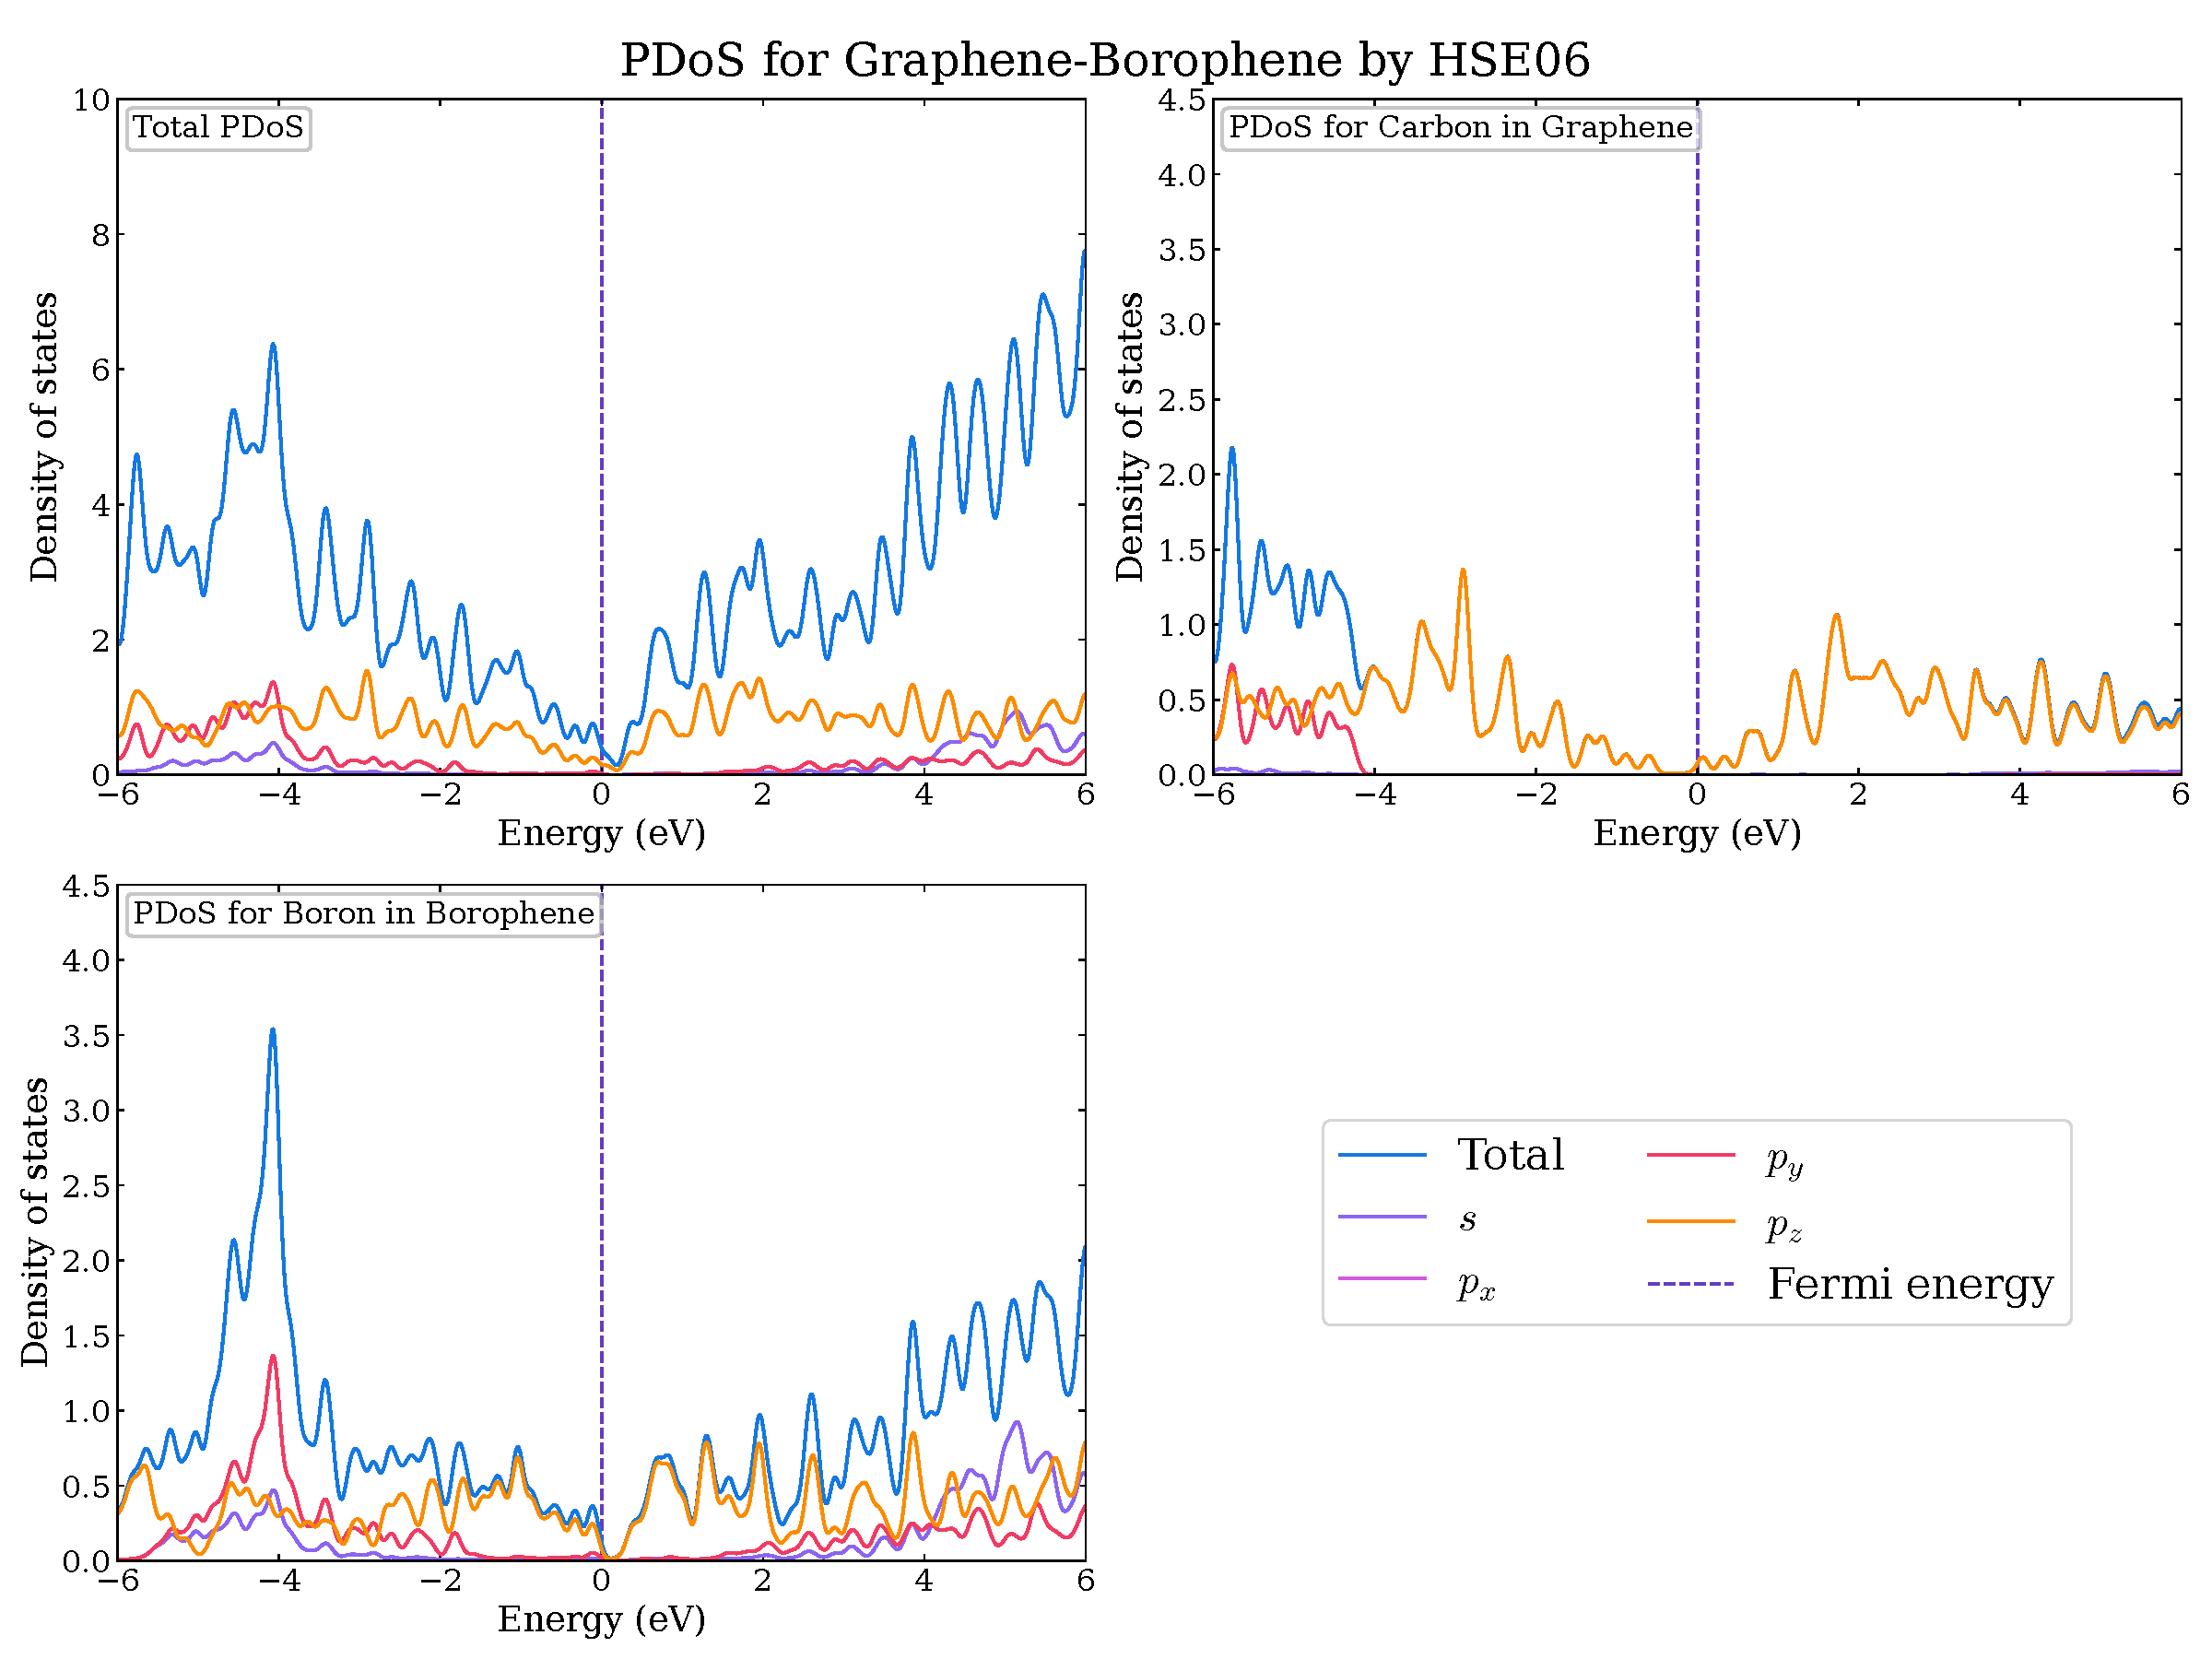
\includegraphics[width=0.80\textwidth]{figures_proj1/S1.9.pdf}
\caption{Projected density of states of the Graphene-Borophene calculated using the HSE06 functional.}
\label{S1.9}
\end{figure}

\begin{figure}[!htbp]
\centering
    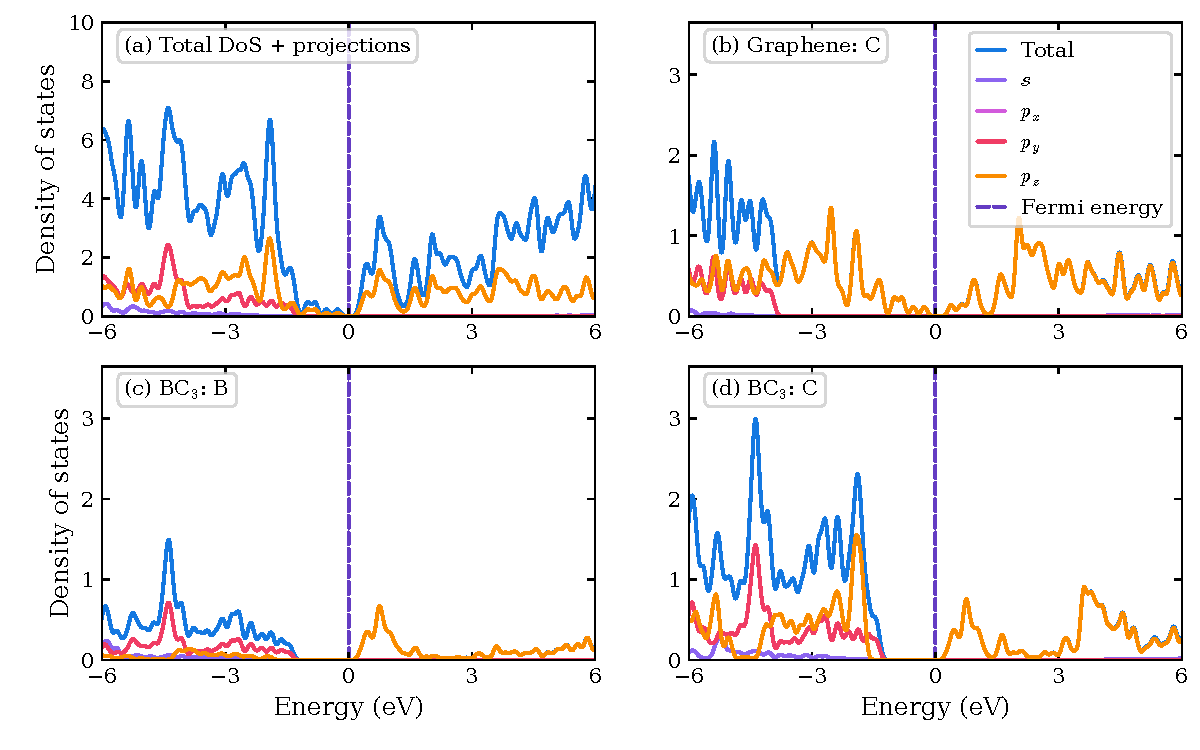
\includegraphics[width=0.80\textwidth]{figures_proj1/S1.10.pdf}
\caption{Projected density of states of the Graphene-\ce{BC3} calculated using the HSE06 functional.}
\label{S1.10}
\end{figure}

\begin{figure}[!htbp]
\centering
    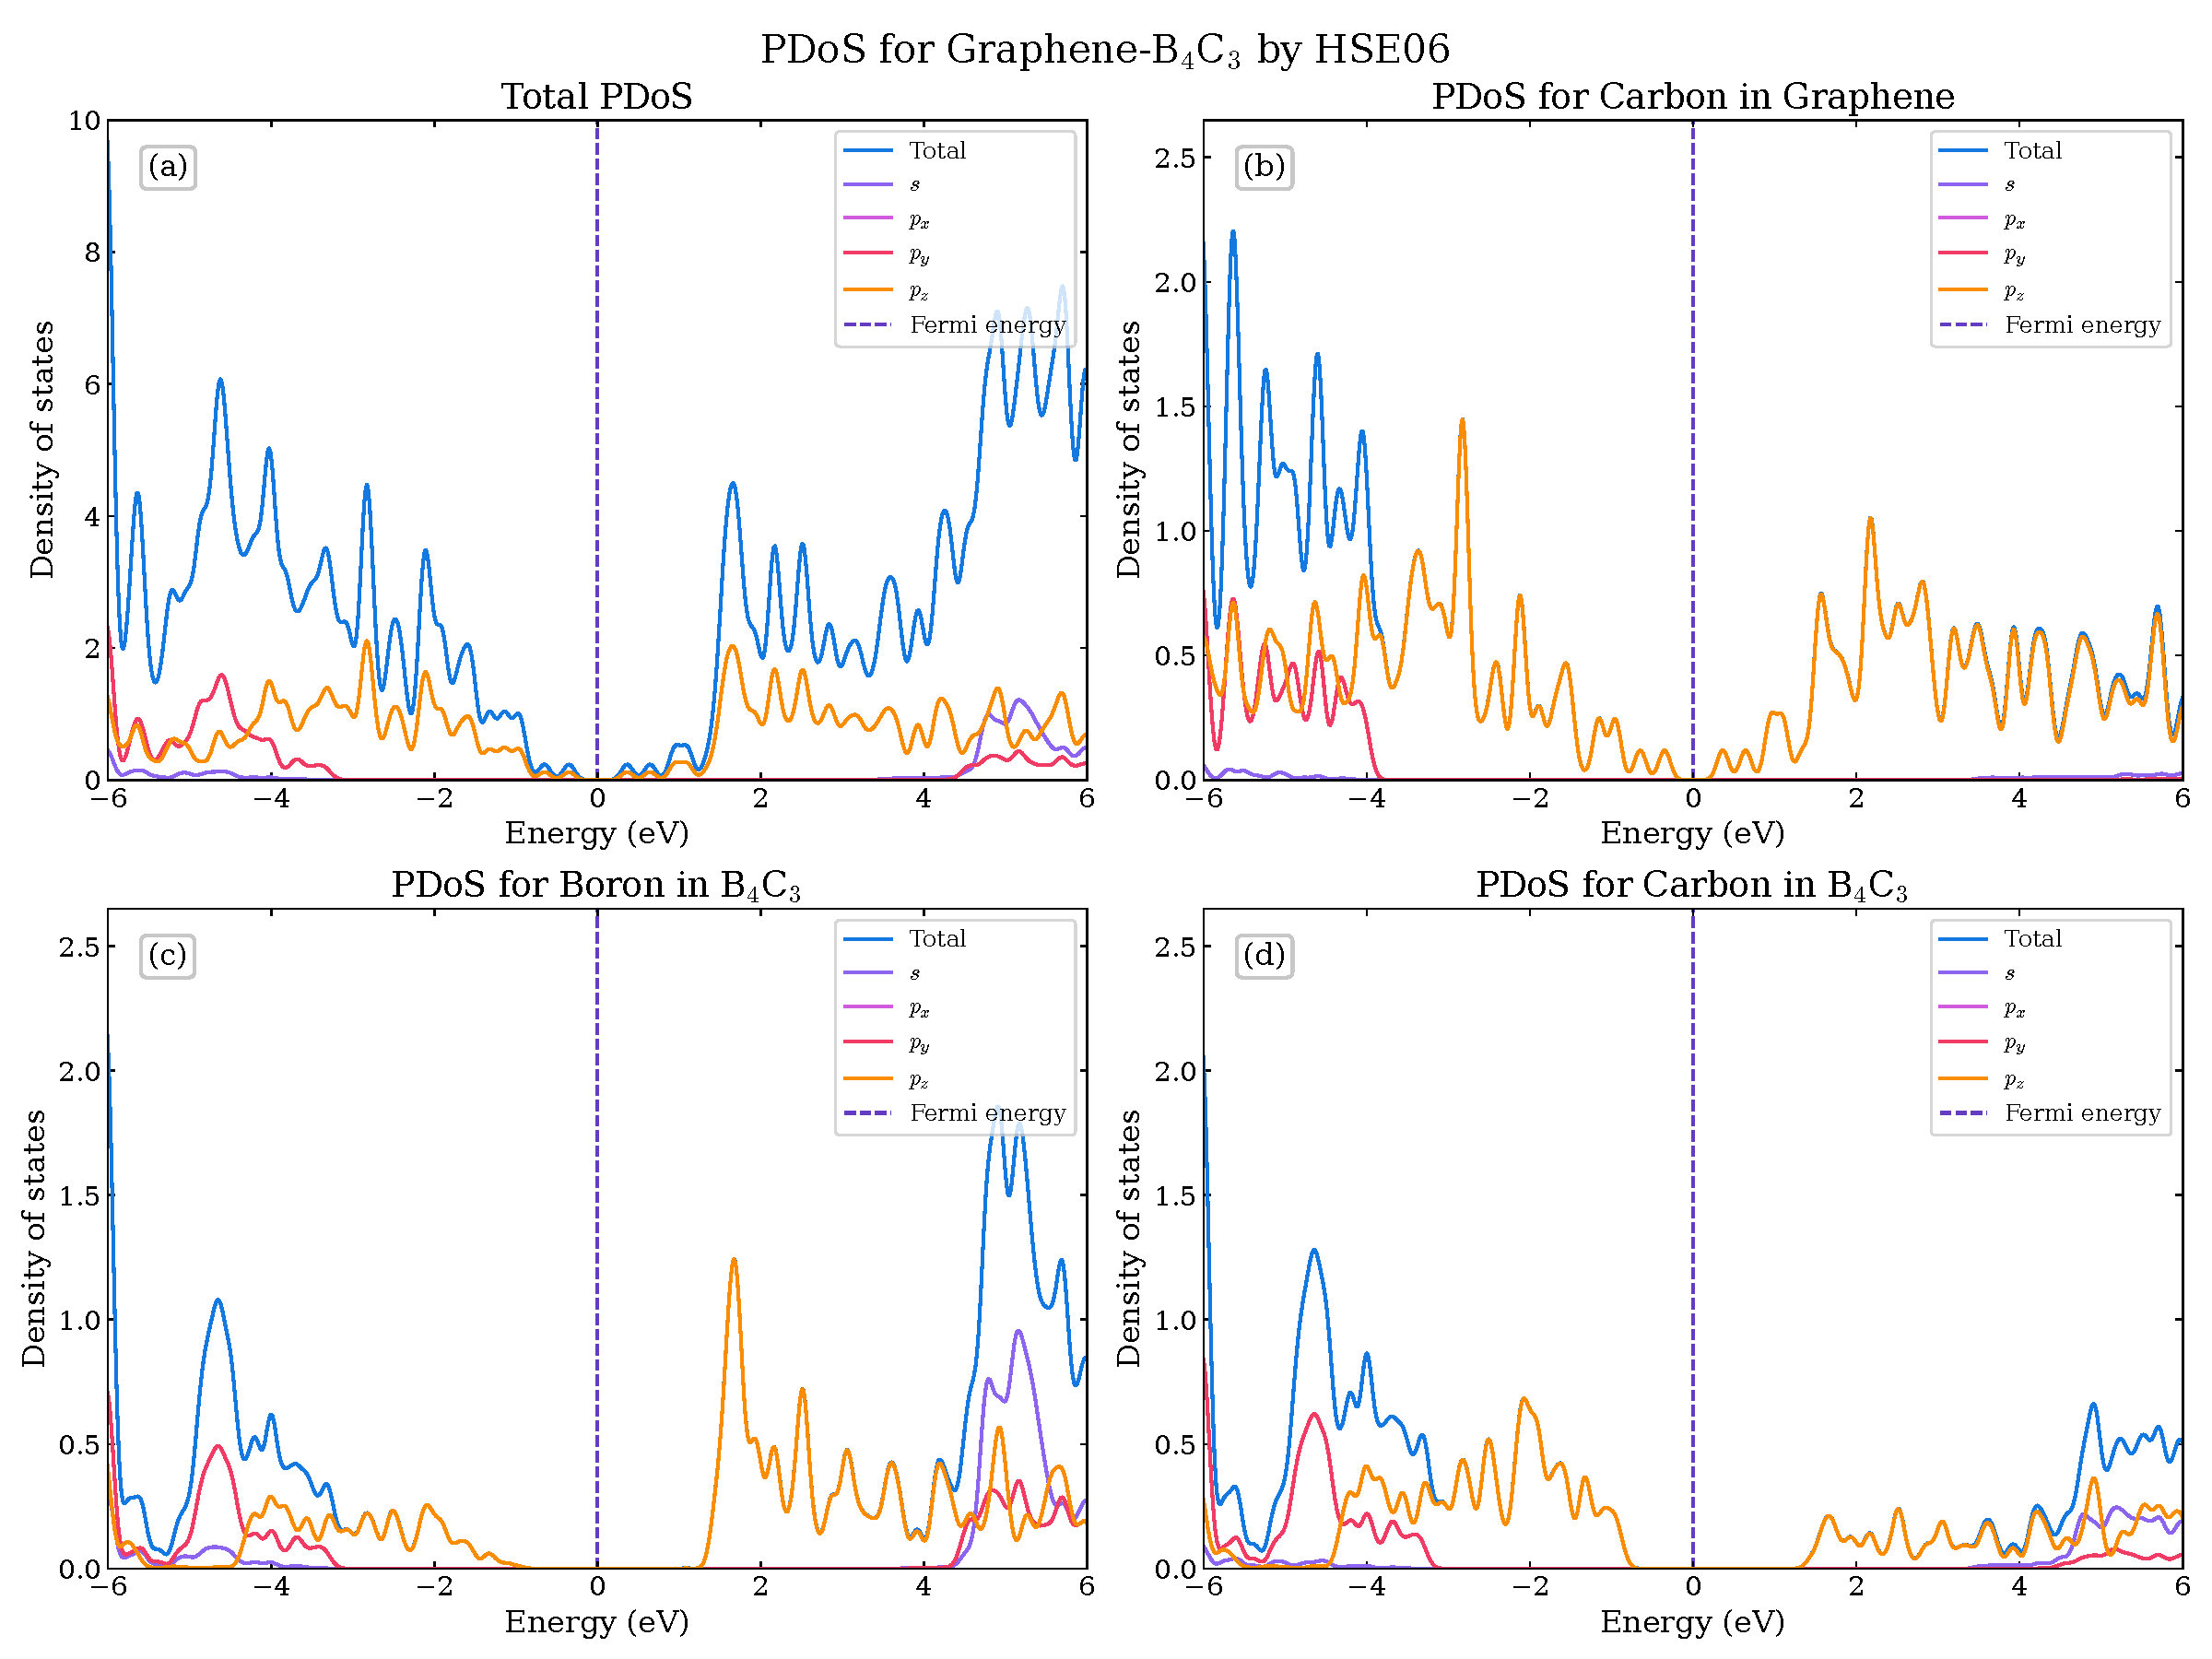
\includegraphics[width=0.80\textwidth]{figures_proj1/S1.11.pdf}
\caption{Projected density of states of the Graphene-\ce{B4C3} calculated using the HSE06 functional.}
\label{S1.11}
\end{figure}

\begin{figure}[!htbp]
\centering
    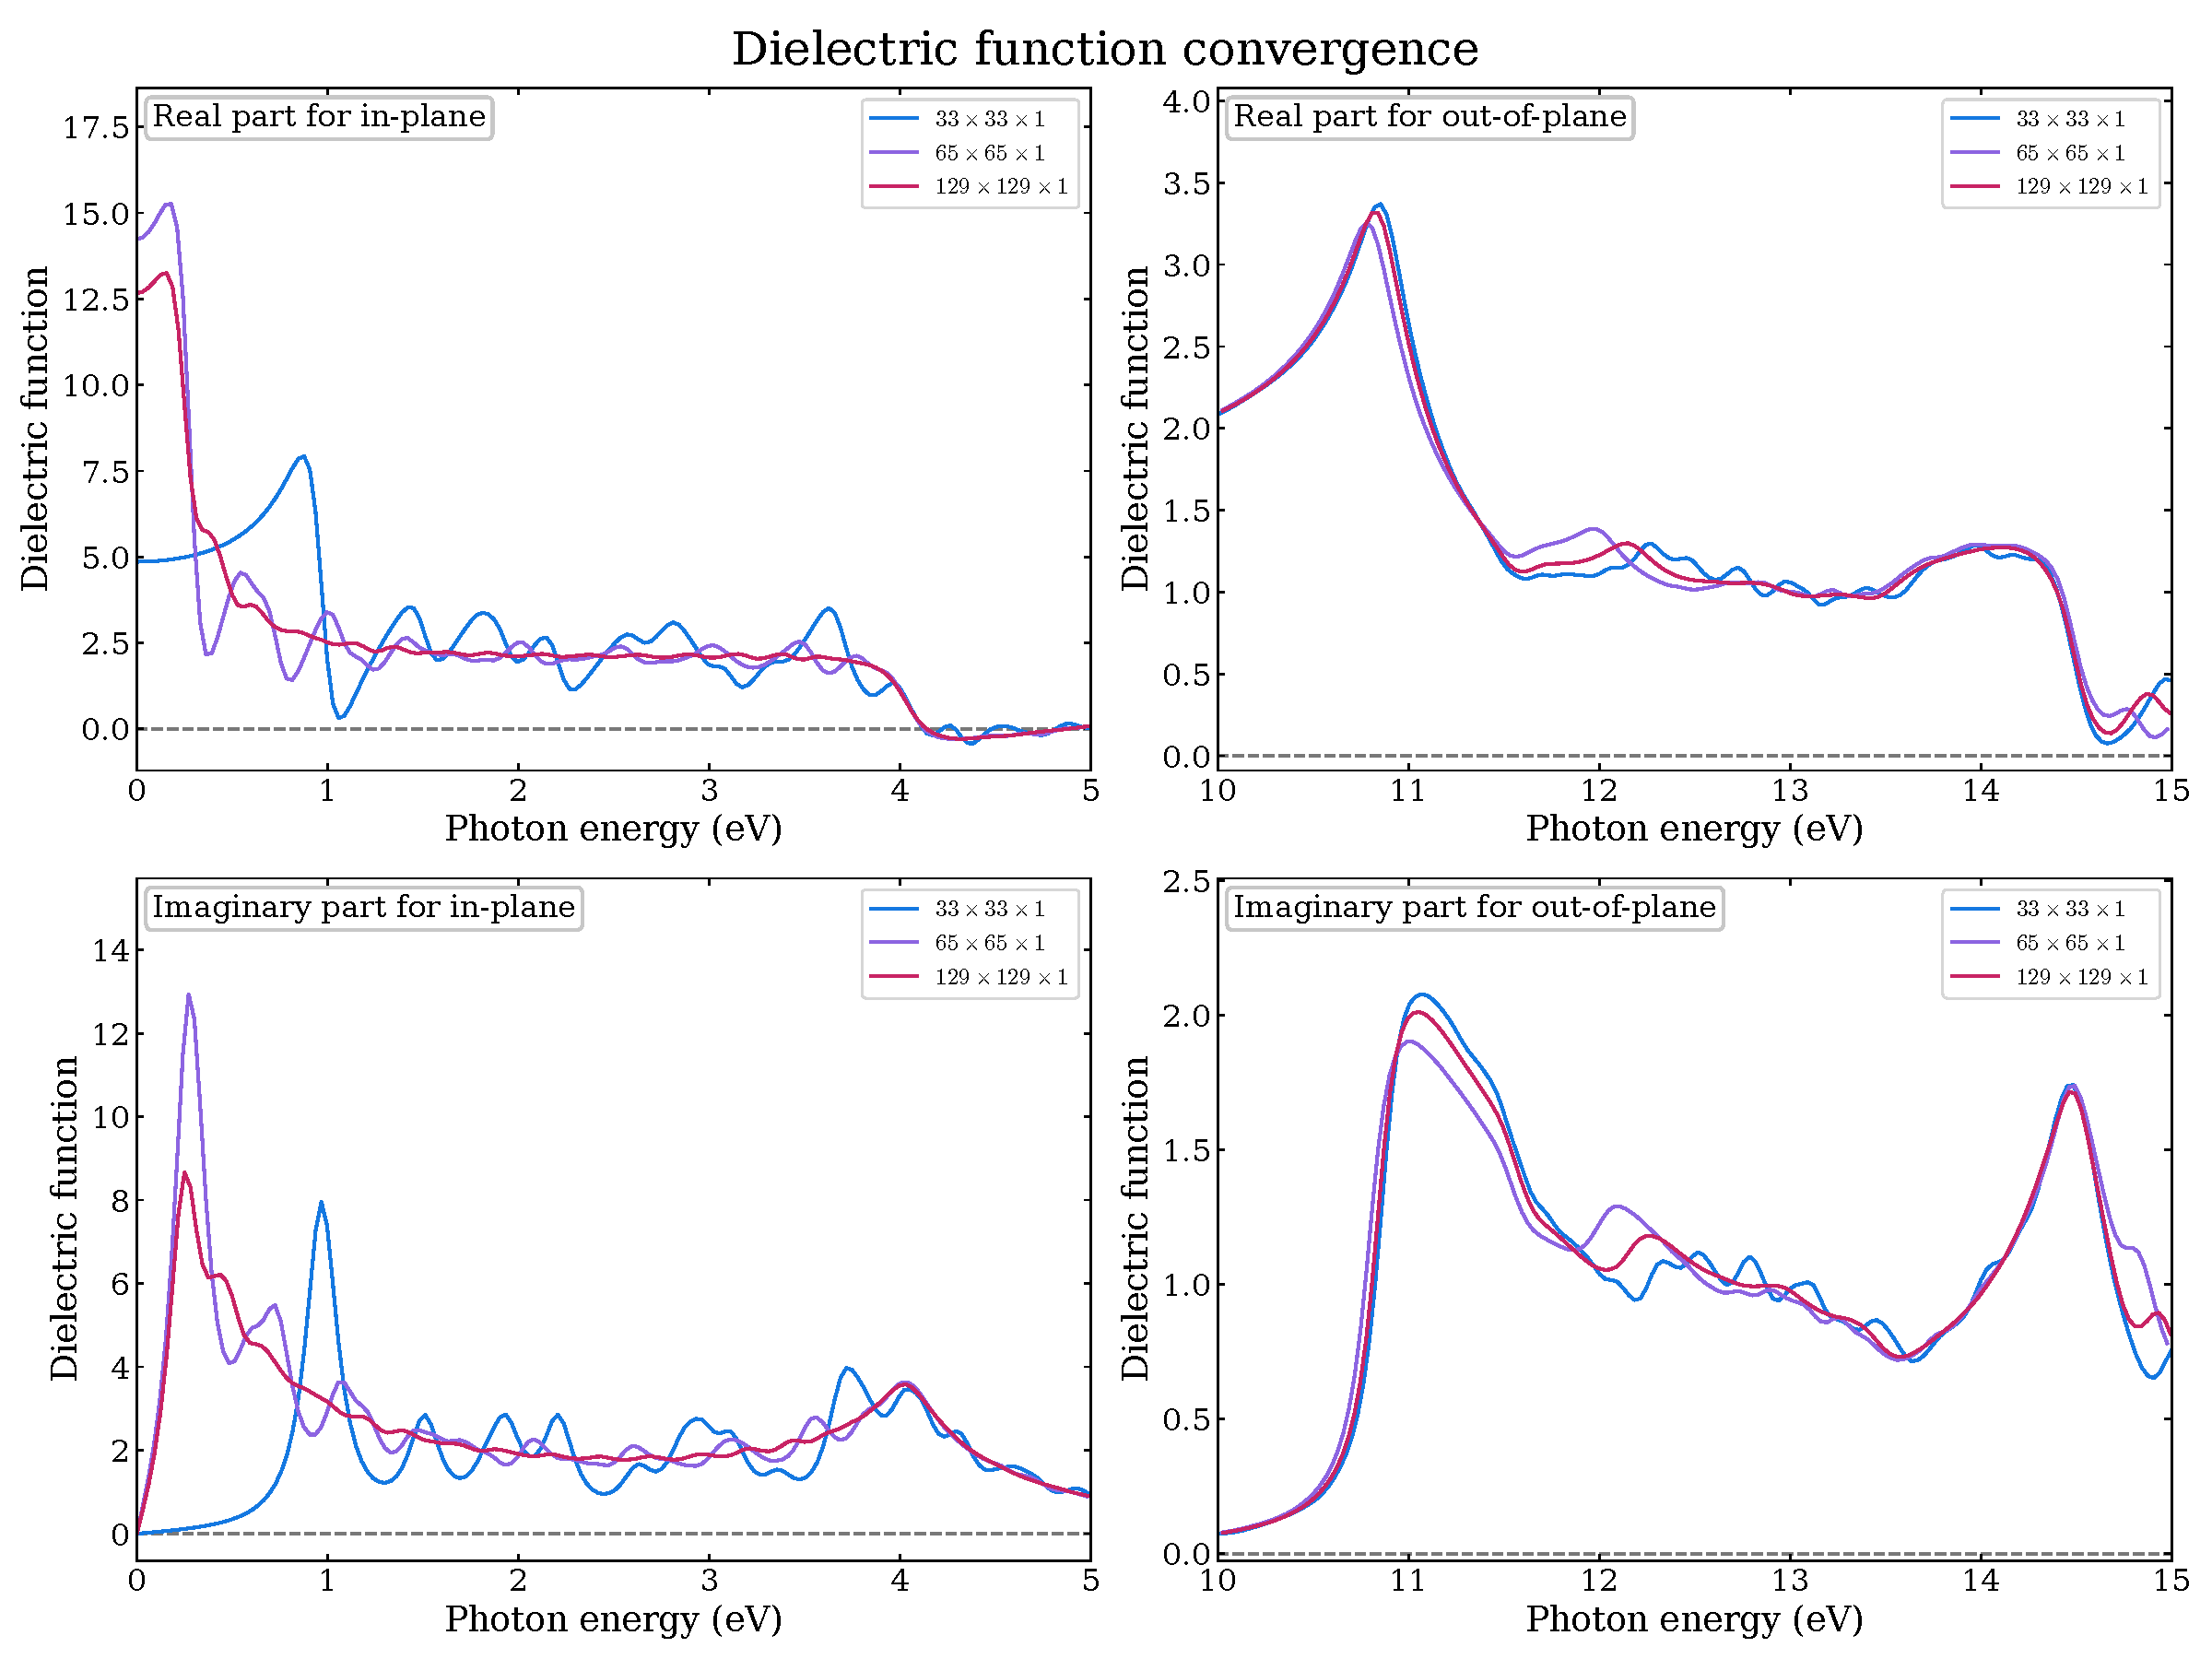
\includegraphics[width=0.80\textwidth]{figures_proj1/S1.12_alt.pdf}
\caption{Dielectric function of graphene calculated using the PBE functional for different k-point meshes;
here, for example,
$33$ denotes a $33 \times 33 \times 1$ k-point mesh.}
\label{S1.12}
\end{figure}

\begin{figure}[!htbp]
\centering
    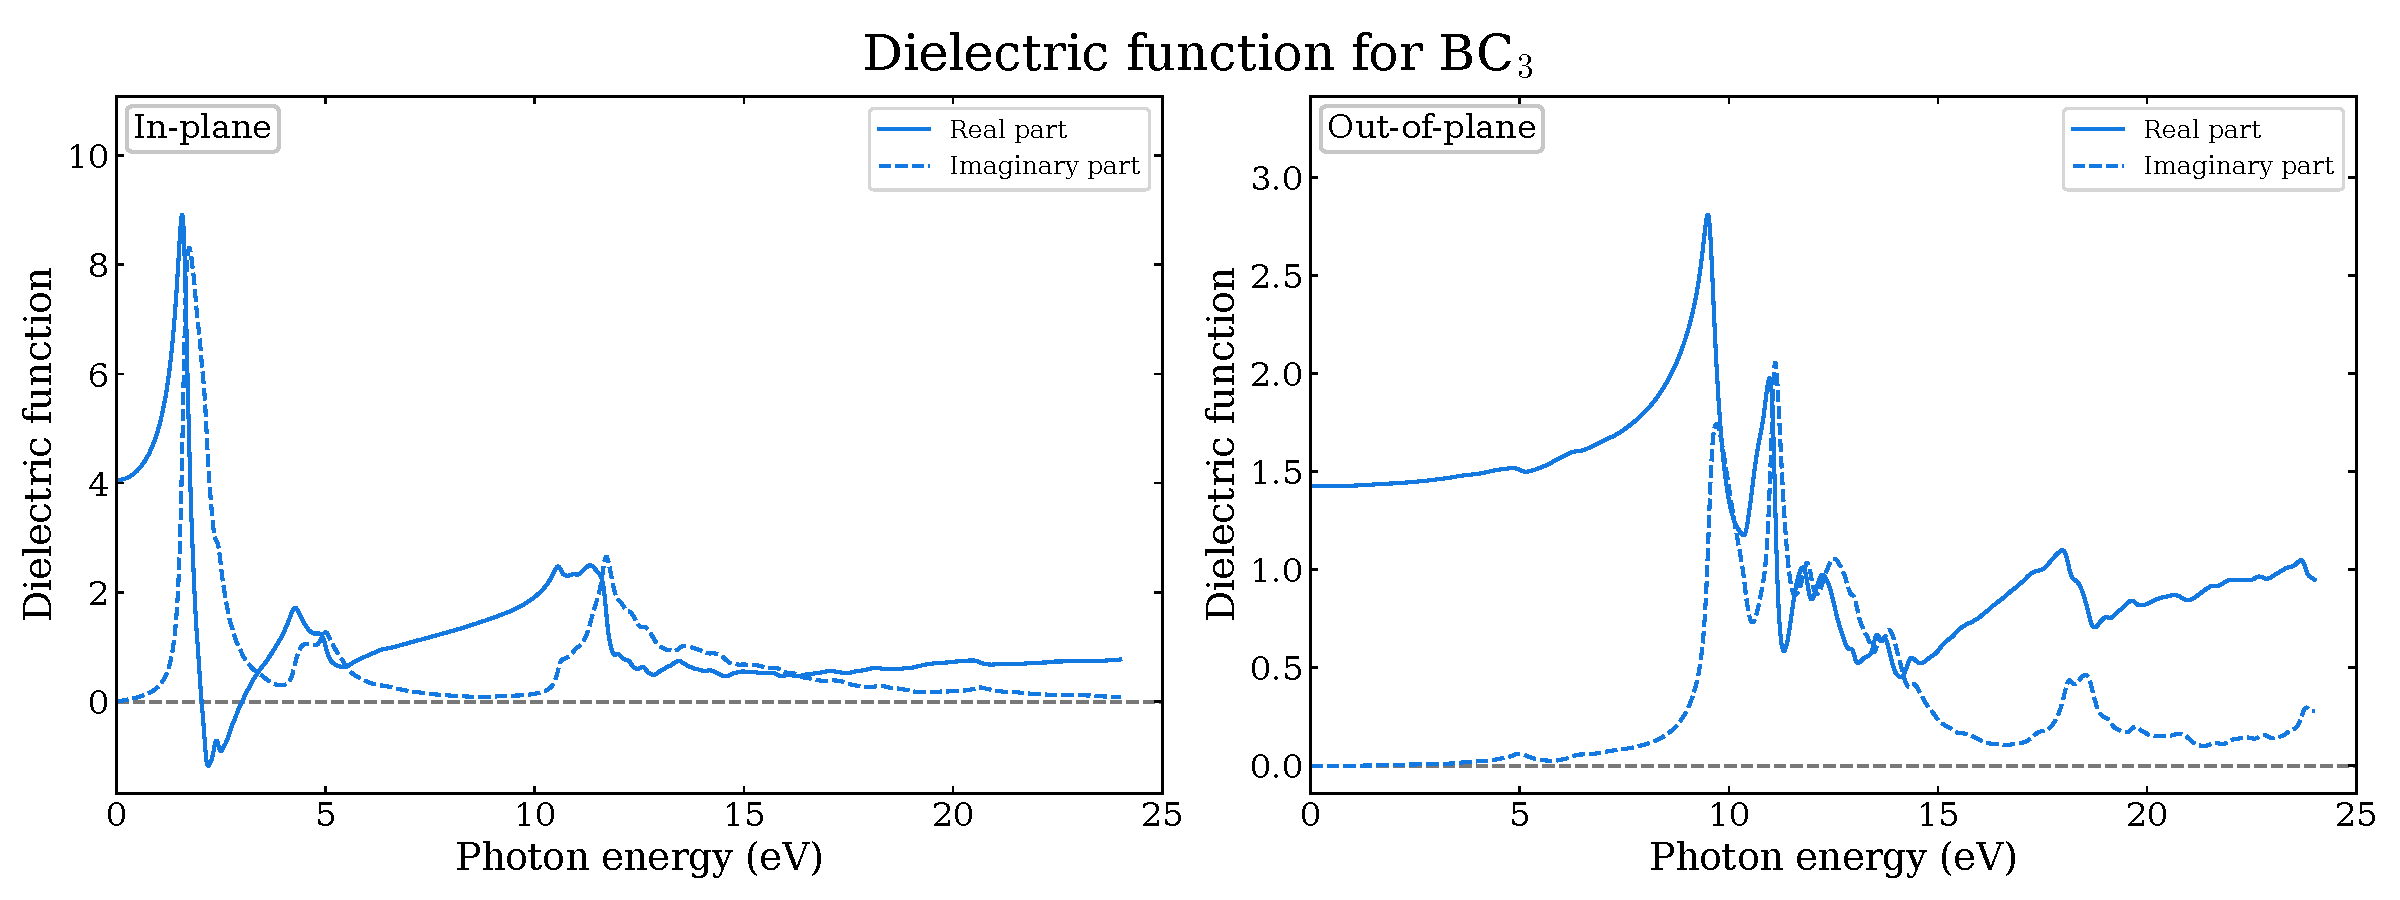
\includegraphics[width=0.80\textwidth]{figures_proj1/S1.13a.pdf}
    \par\nointerlineskip
    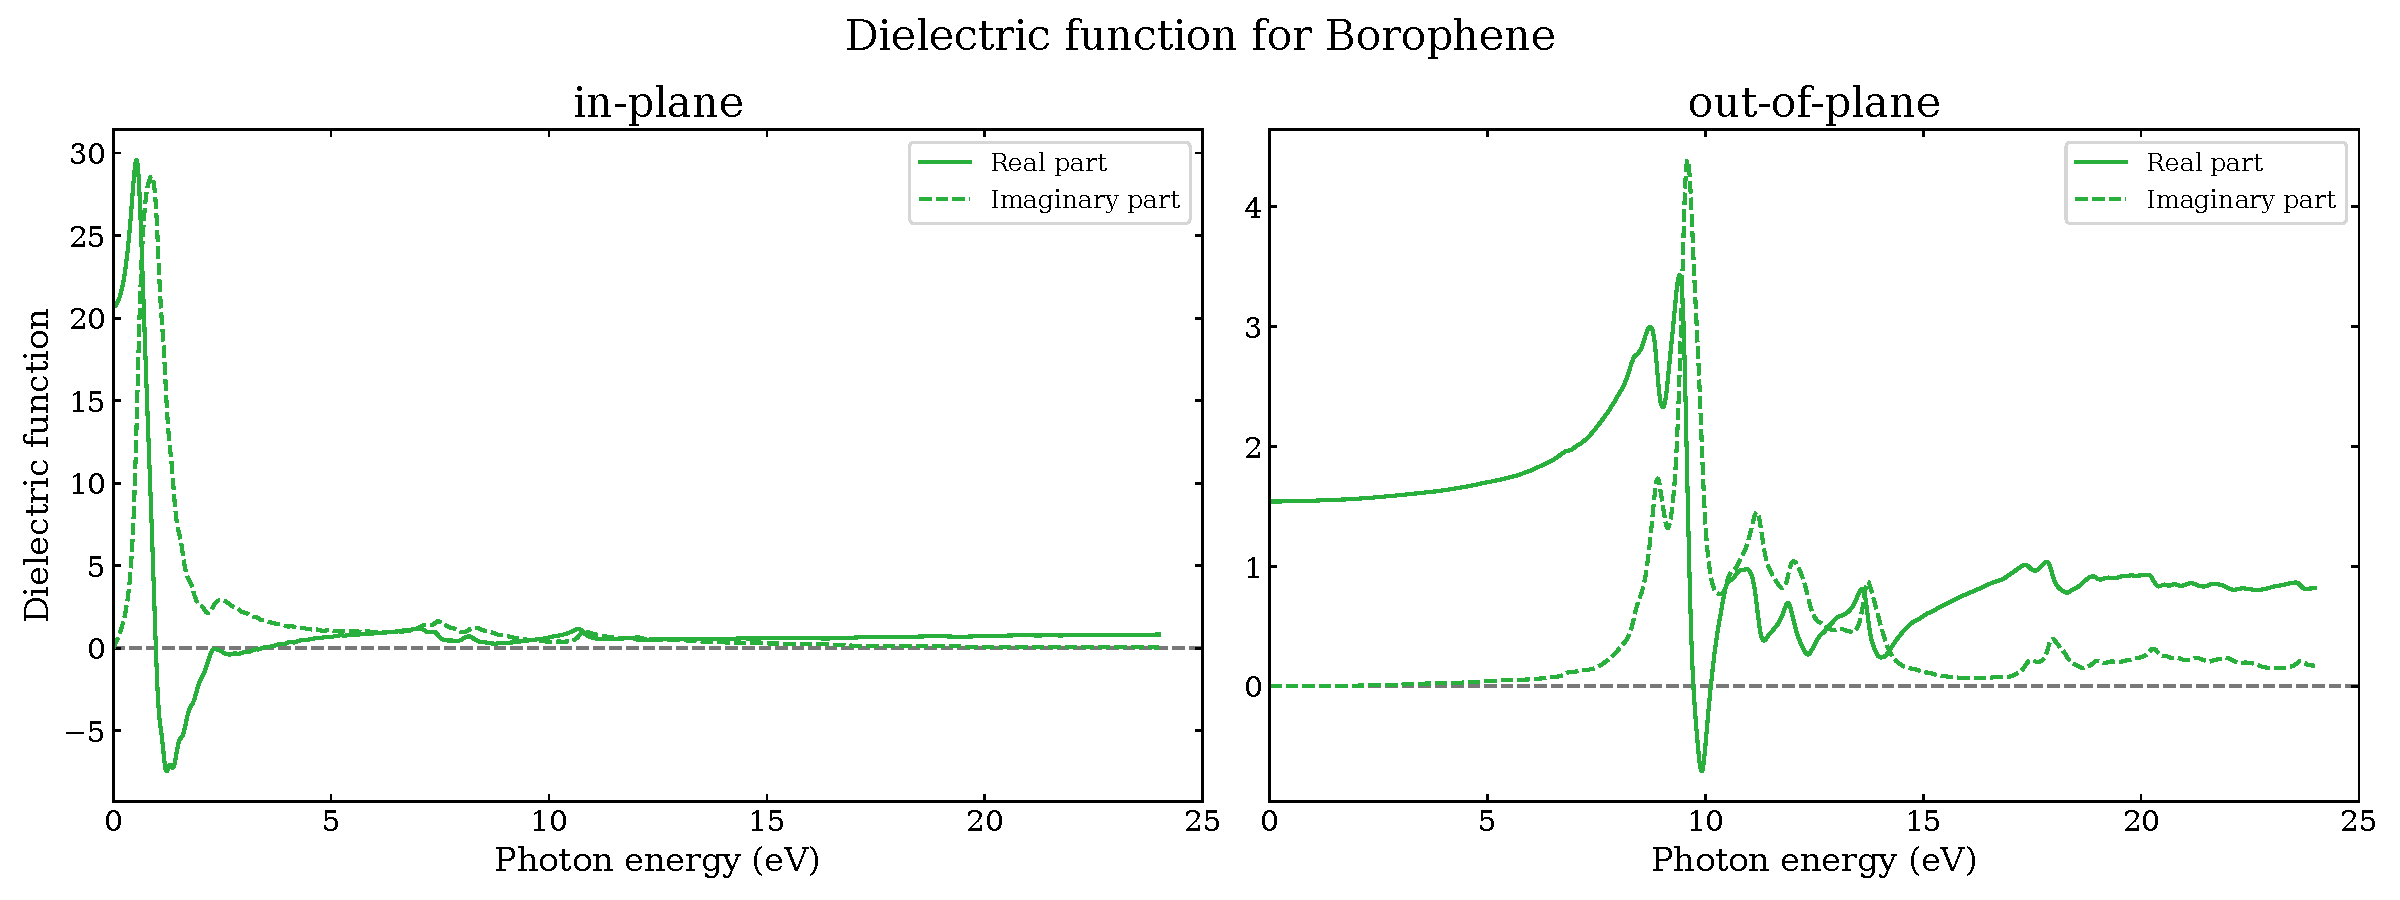
\includegraphics[width=0.80\textwidth]{figures_proj1/S1.13b.pdf}
    \par\nointerlineskip
    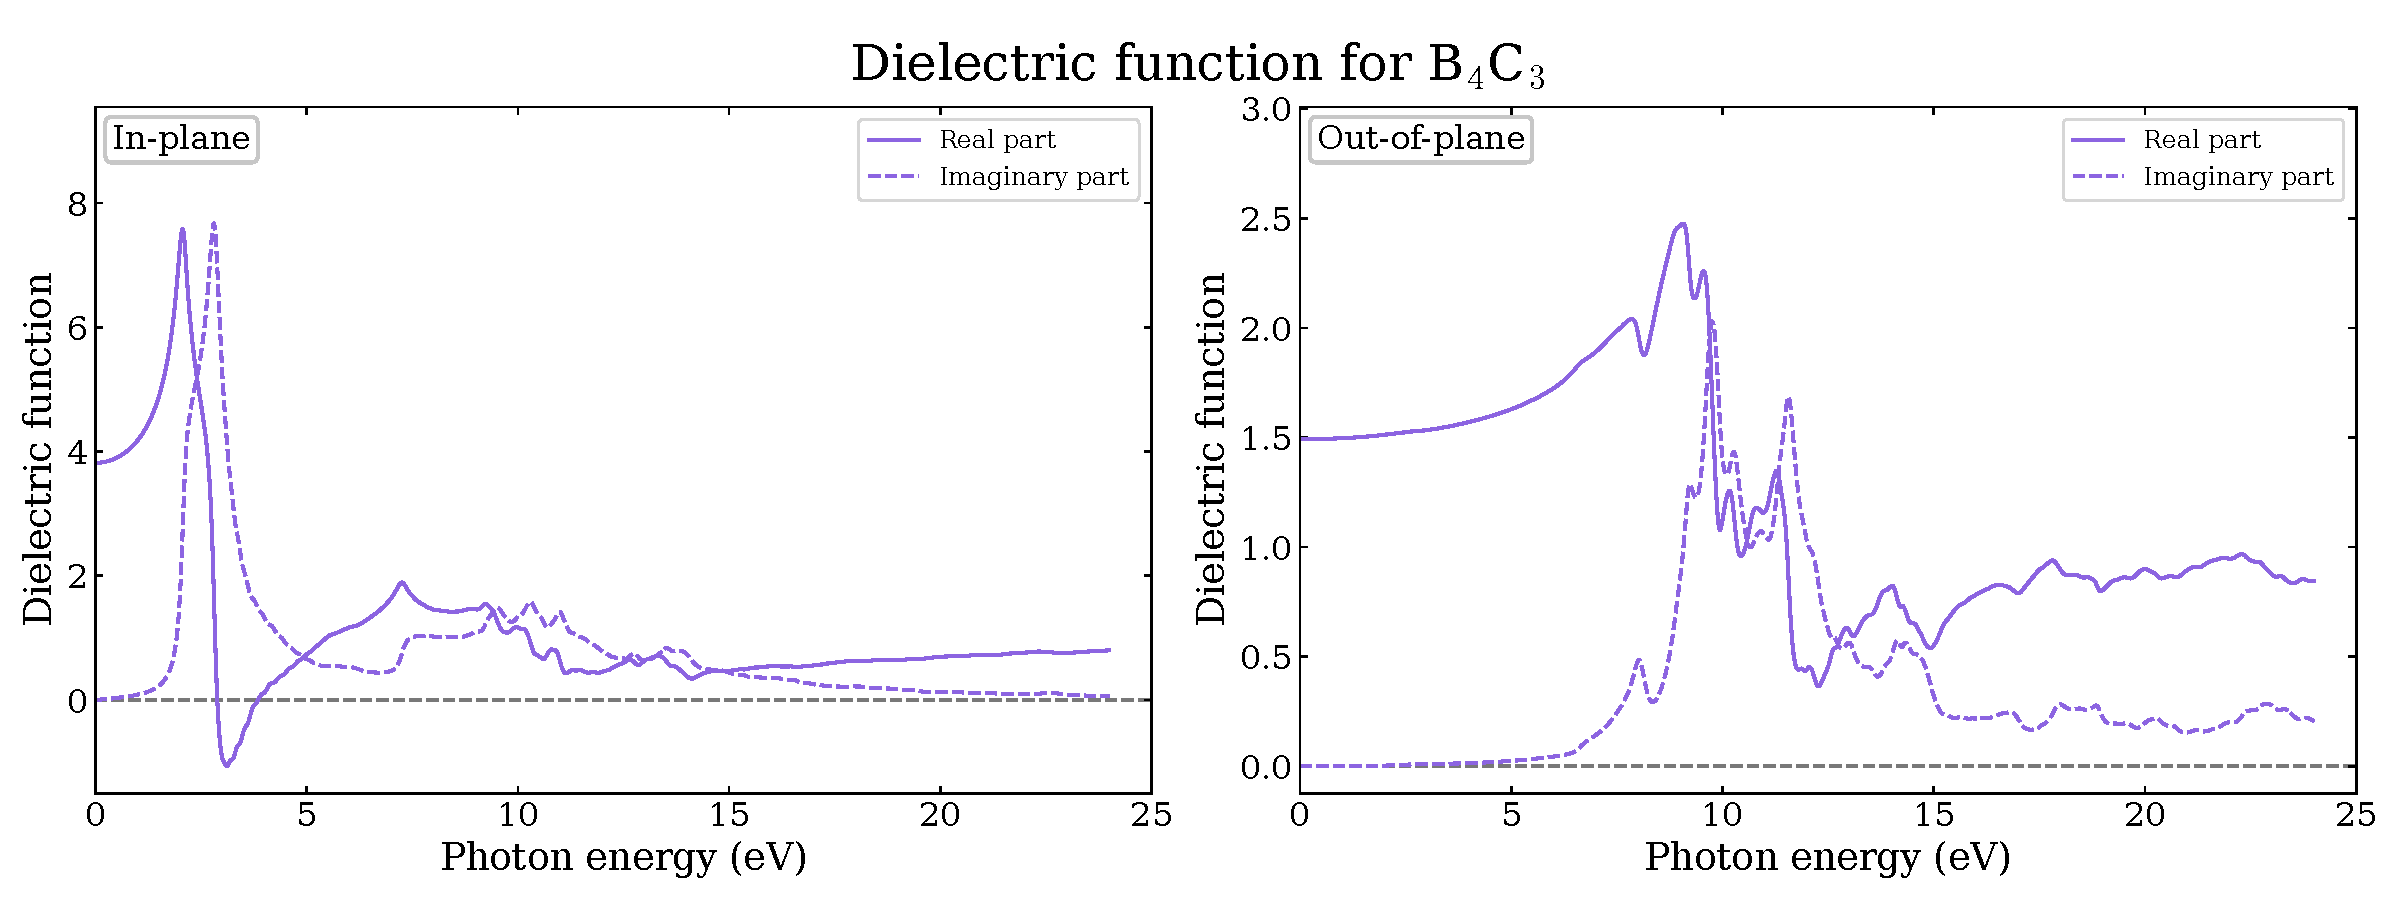
\includegraphics[width=0.80\textwidth]{figures_proj1/S1.13c.pdf}
    \par\nointerlineskip
    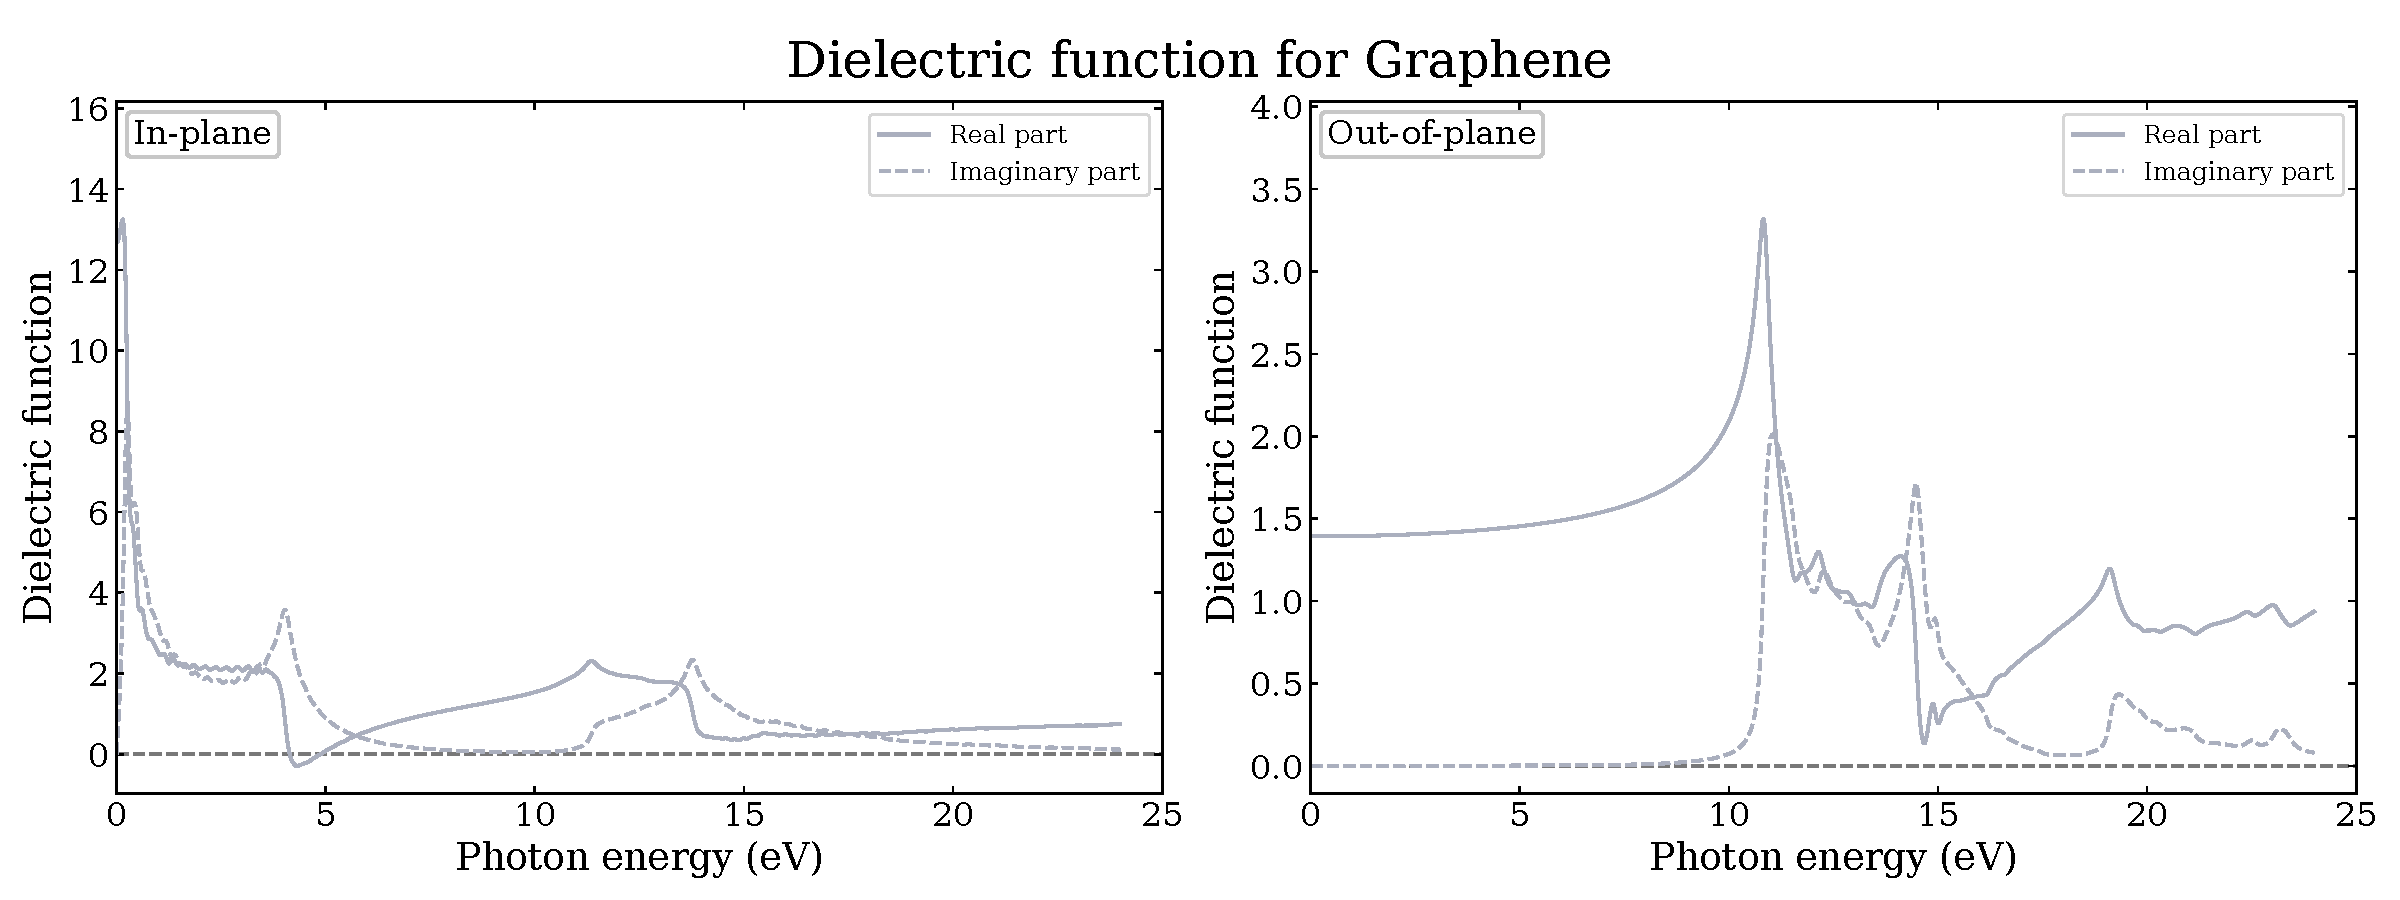
\includegraphics[width=0.80\textwidth]{figures_proj1/S1.13d.pdf}
\caption{Real and imaginary parts of the dielectric function
for the four monolayers as calculated using the PBE functional with a
$129\times 129\times 1$
k-point mesh for graphene,
and a $65\times 65\times 1$
k-point mesh for the borophene and boron-carbide monolayers.
Solid and dashed lines denote the real and imaginary parts, respectively.}
\label{S1.13}
\end{figure}

\begin{figure}[!htbp]
\centering
    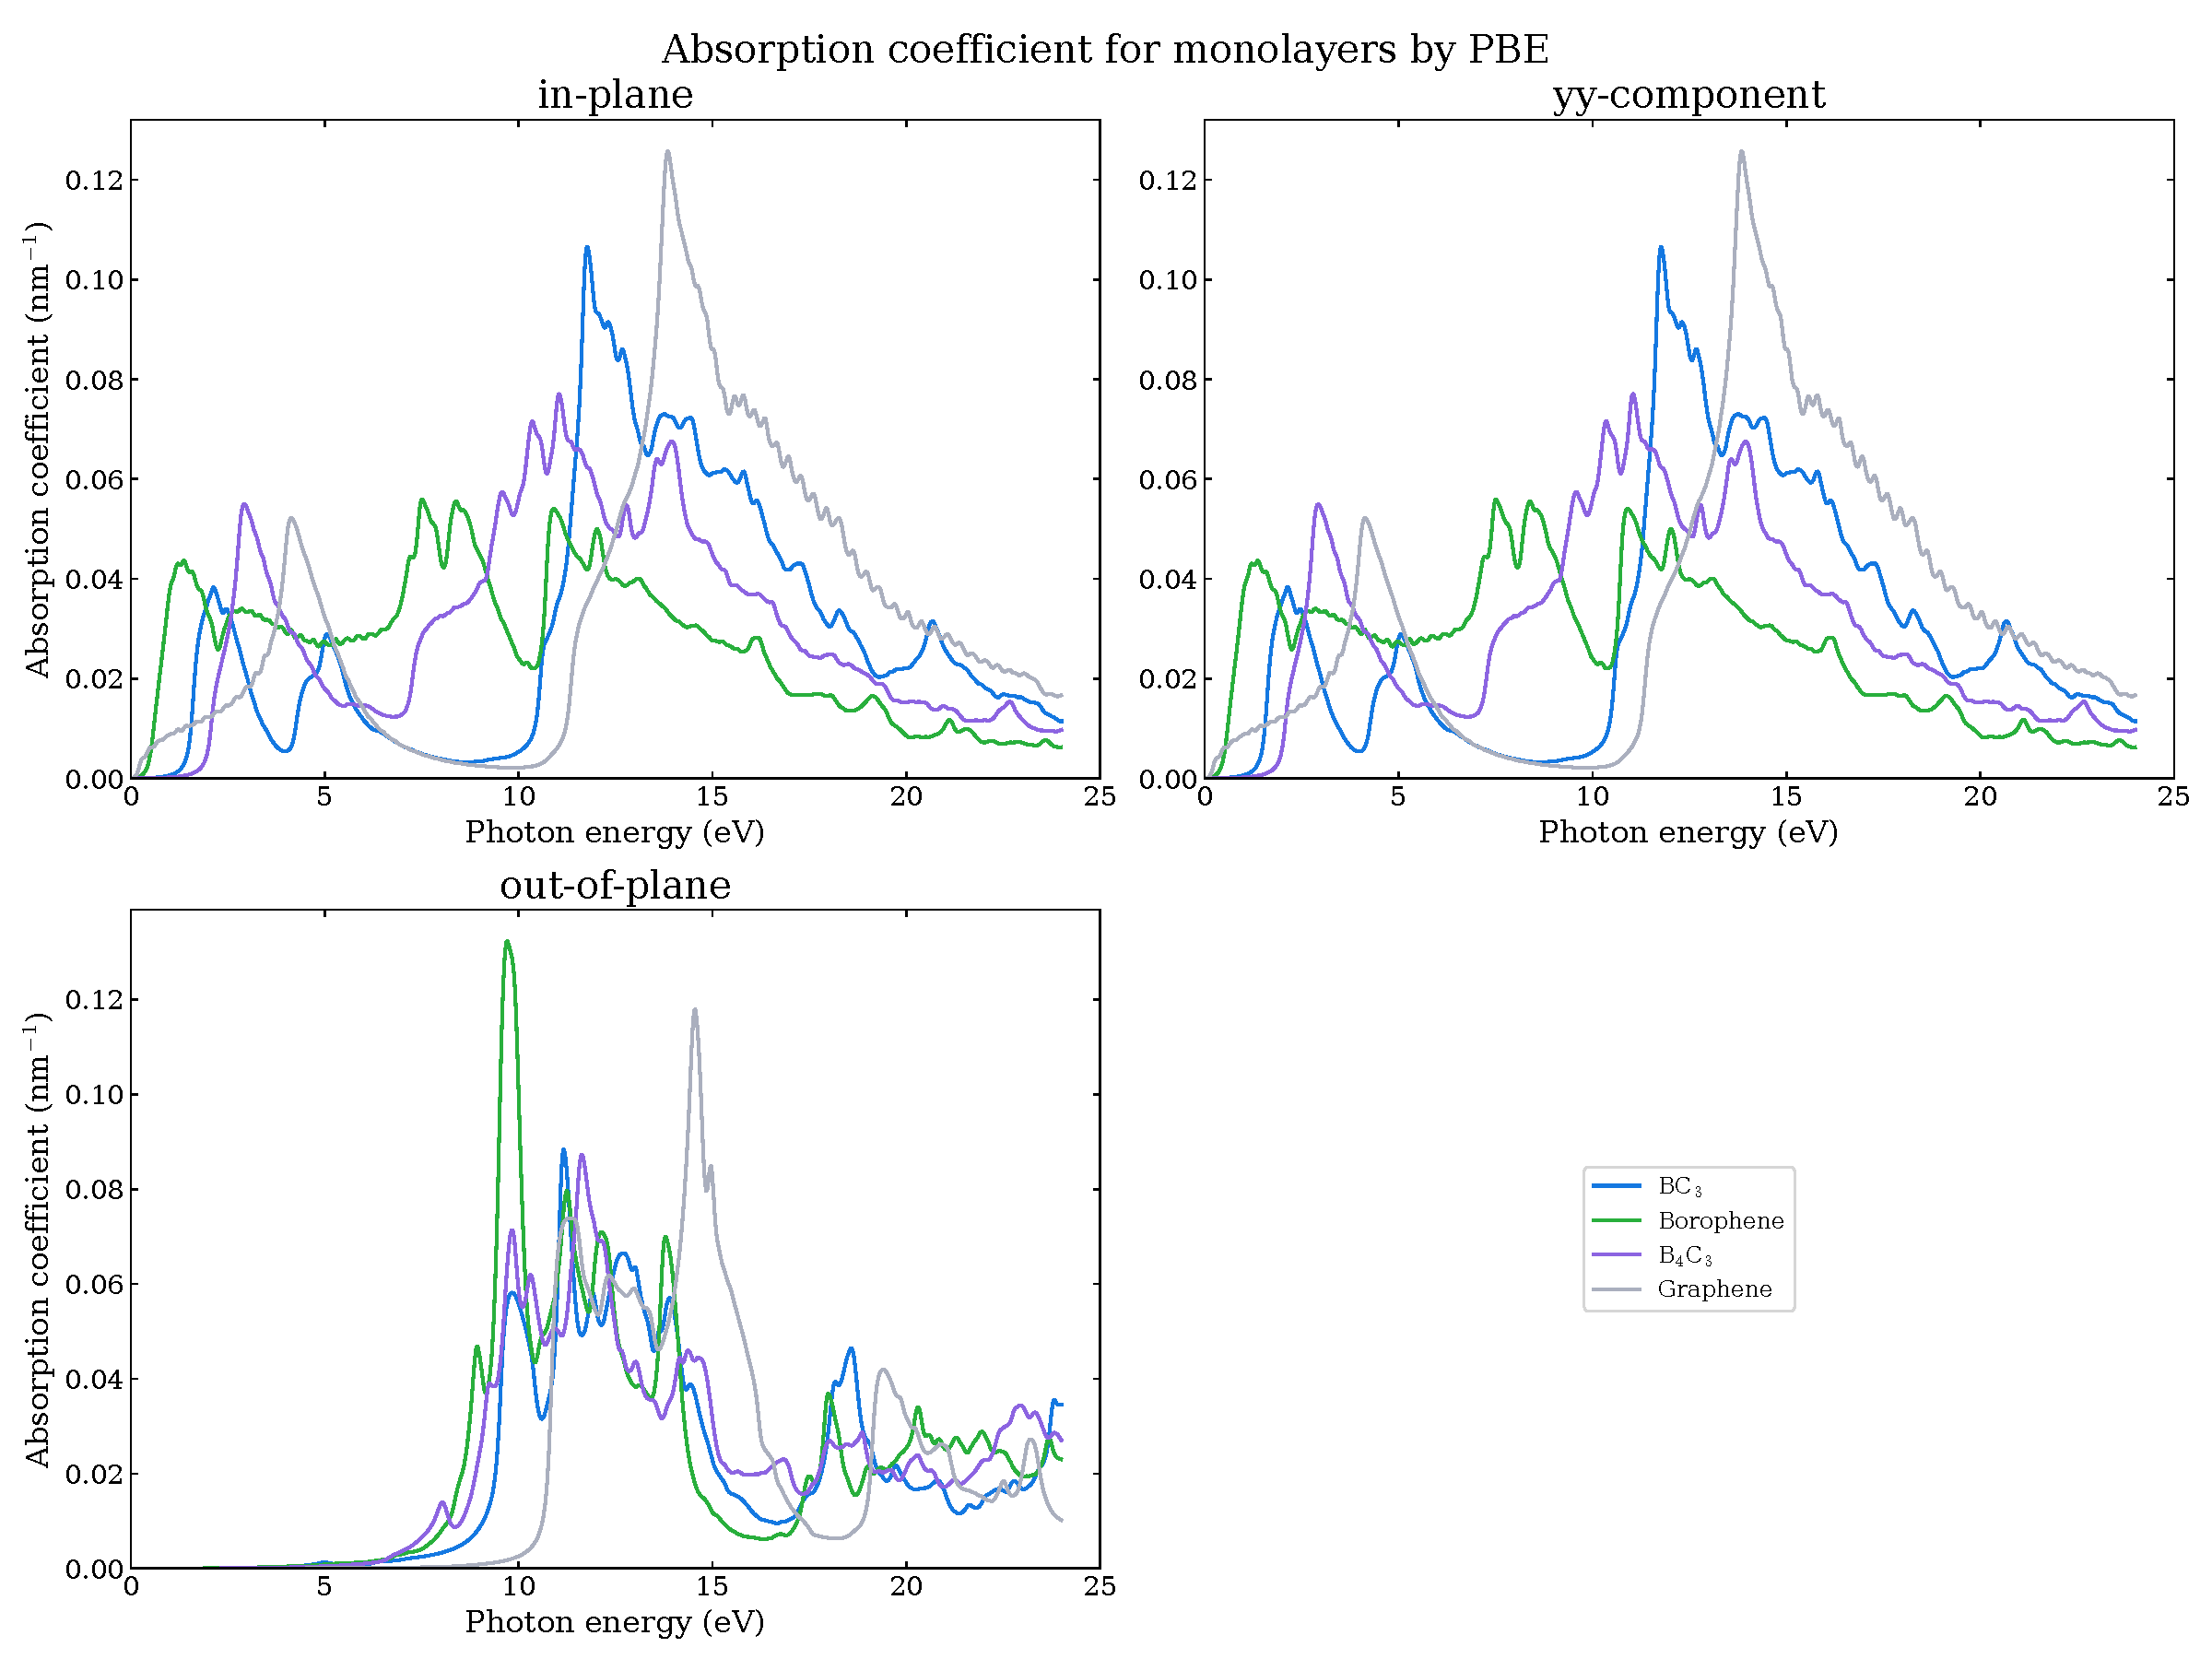
\includegraphics[width=0.80\textwidth]{figures_proj1/S1.14a.pdf}
    \par\nointerlineskip
    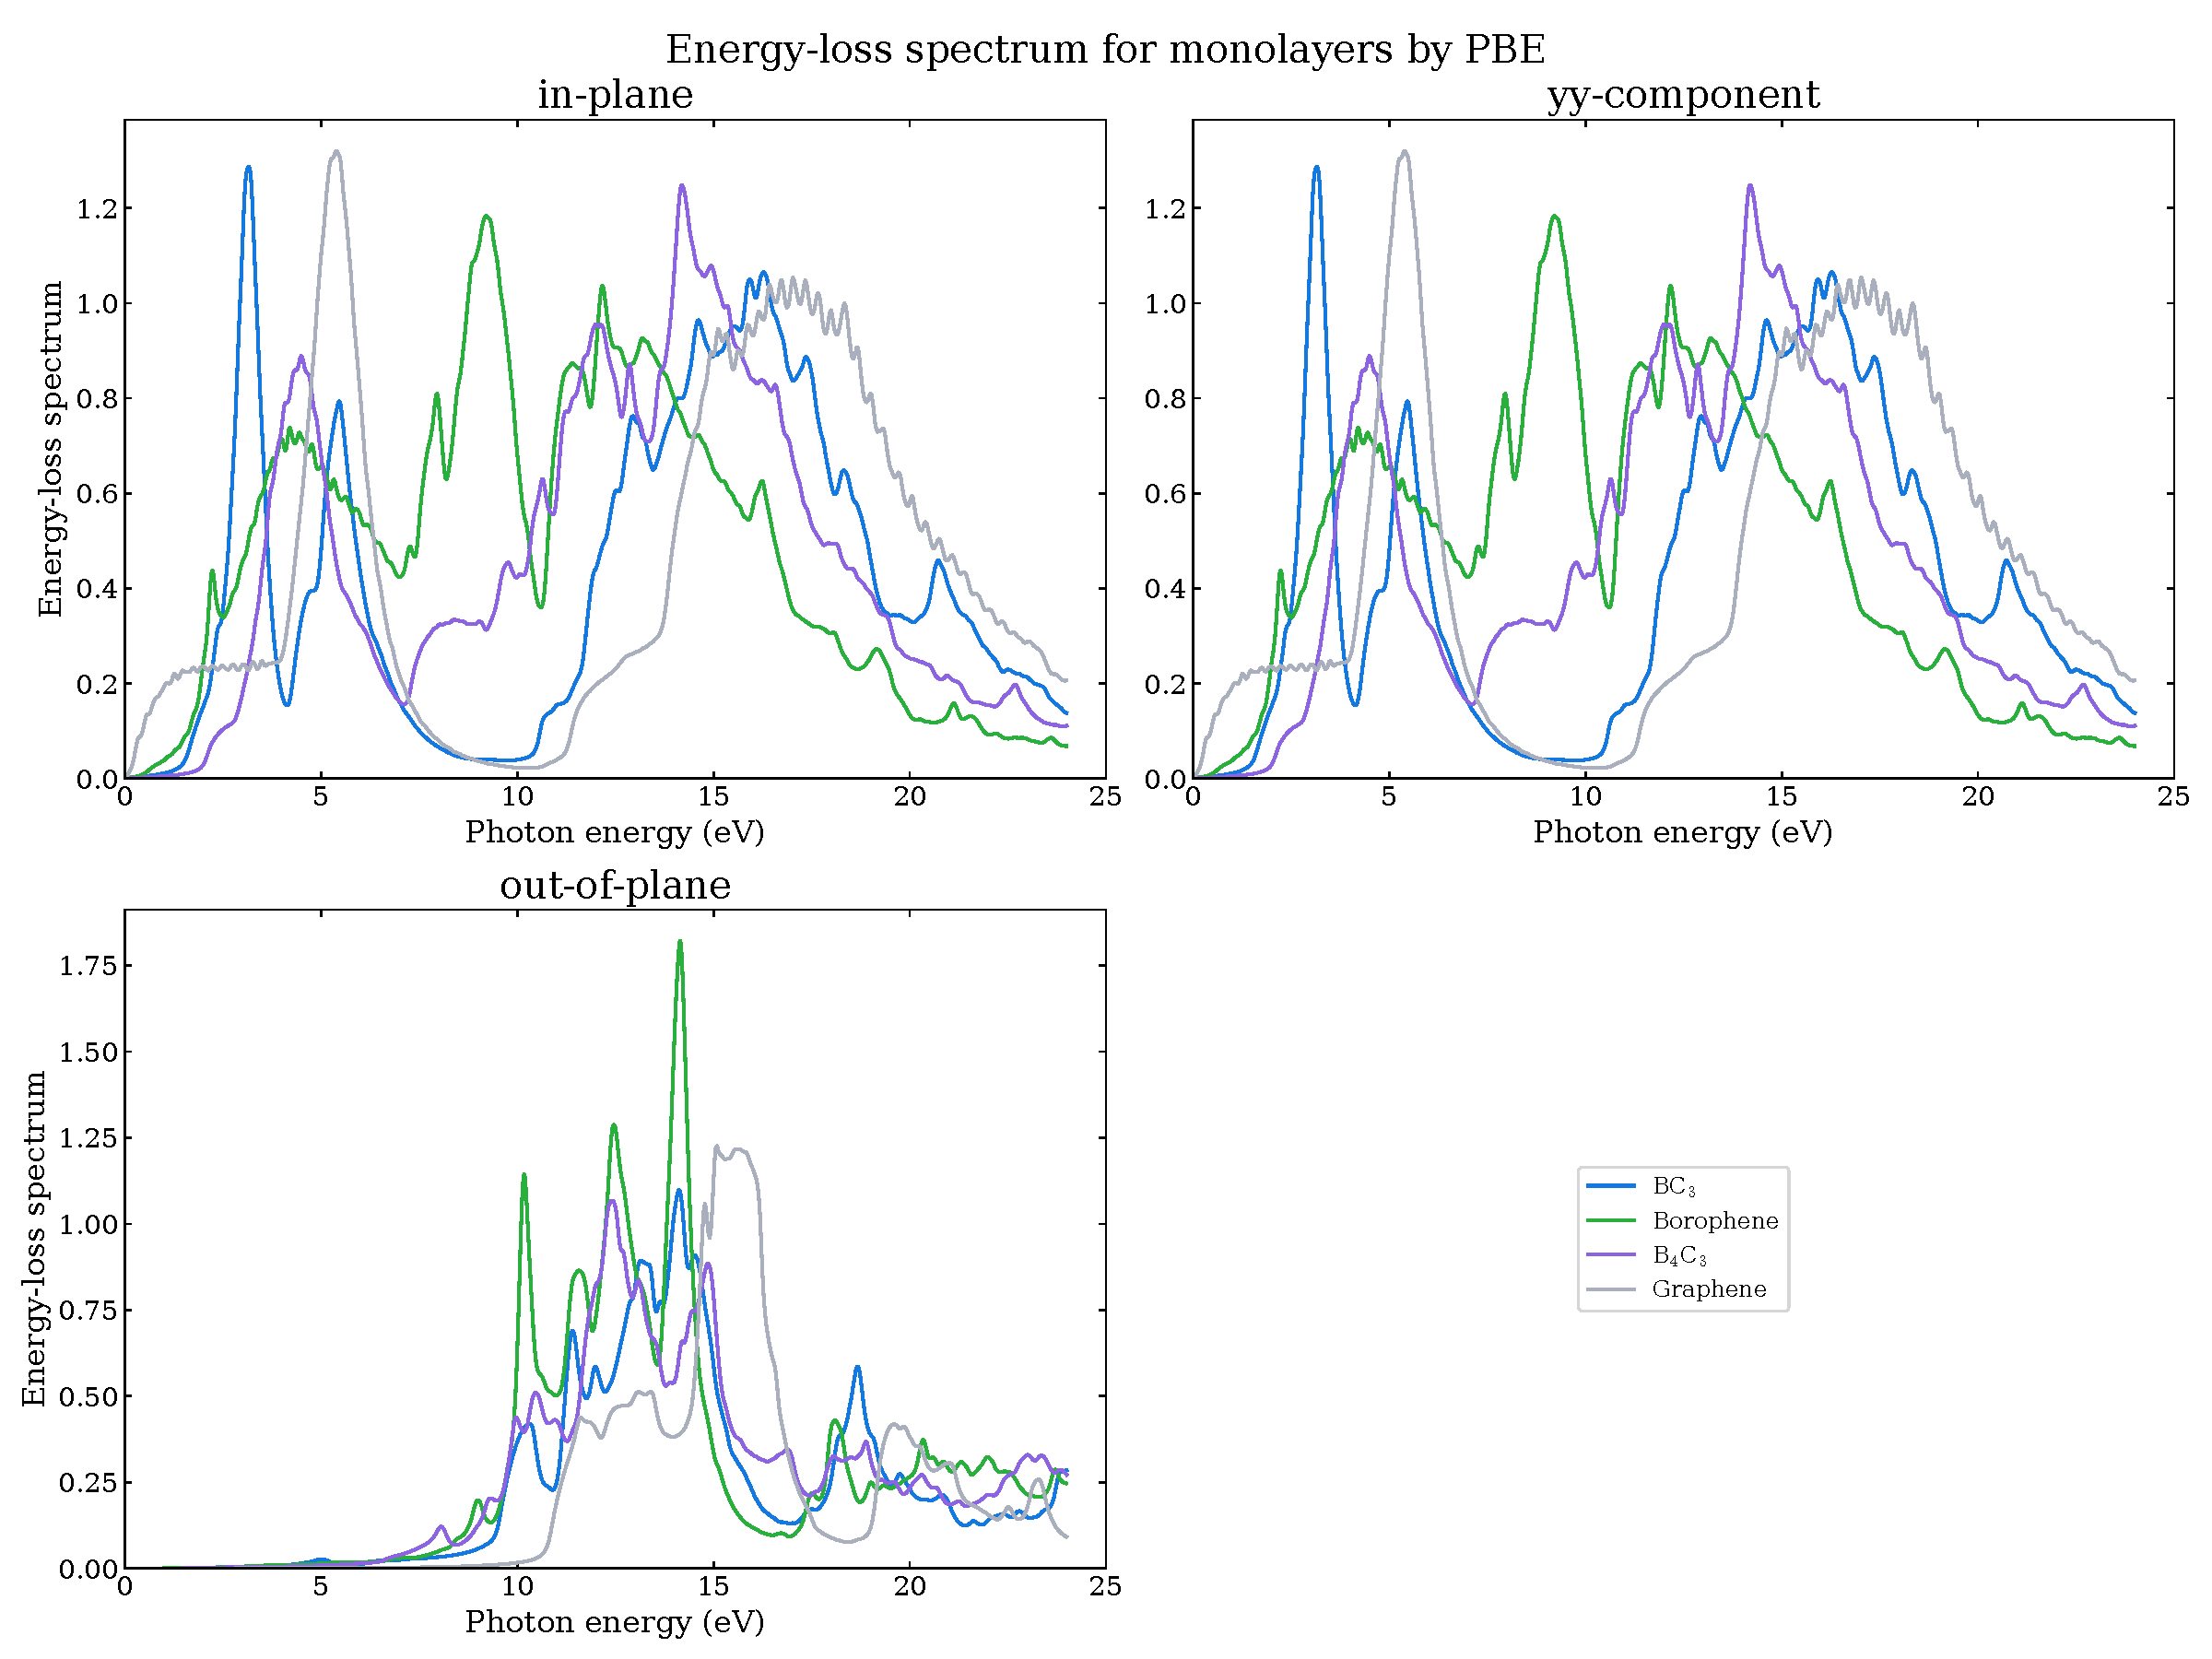
\includegraphics[width=0.80\textwidth]{figures_proj1/S1.14b.pdf}
\caption[Optical properties of the four monolayers calculated using PBE.]{Optical properties of the four monolayers calculated using PBE with the k-point meshes specified in figure~\ref{S1.13}.
Upper: Absorption coefficient in \si{\per\nano\metre}; lower: Dimensionless energy-loss spectrum.}
\label{S1.14}
\end{figure}

\begin{figure}[!htbp]
\ContinuedFloat
\centering
    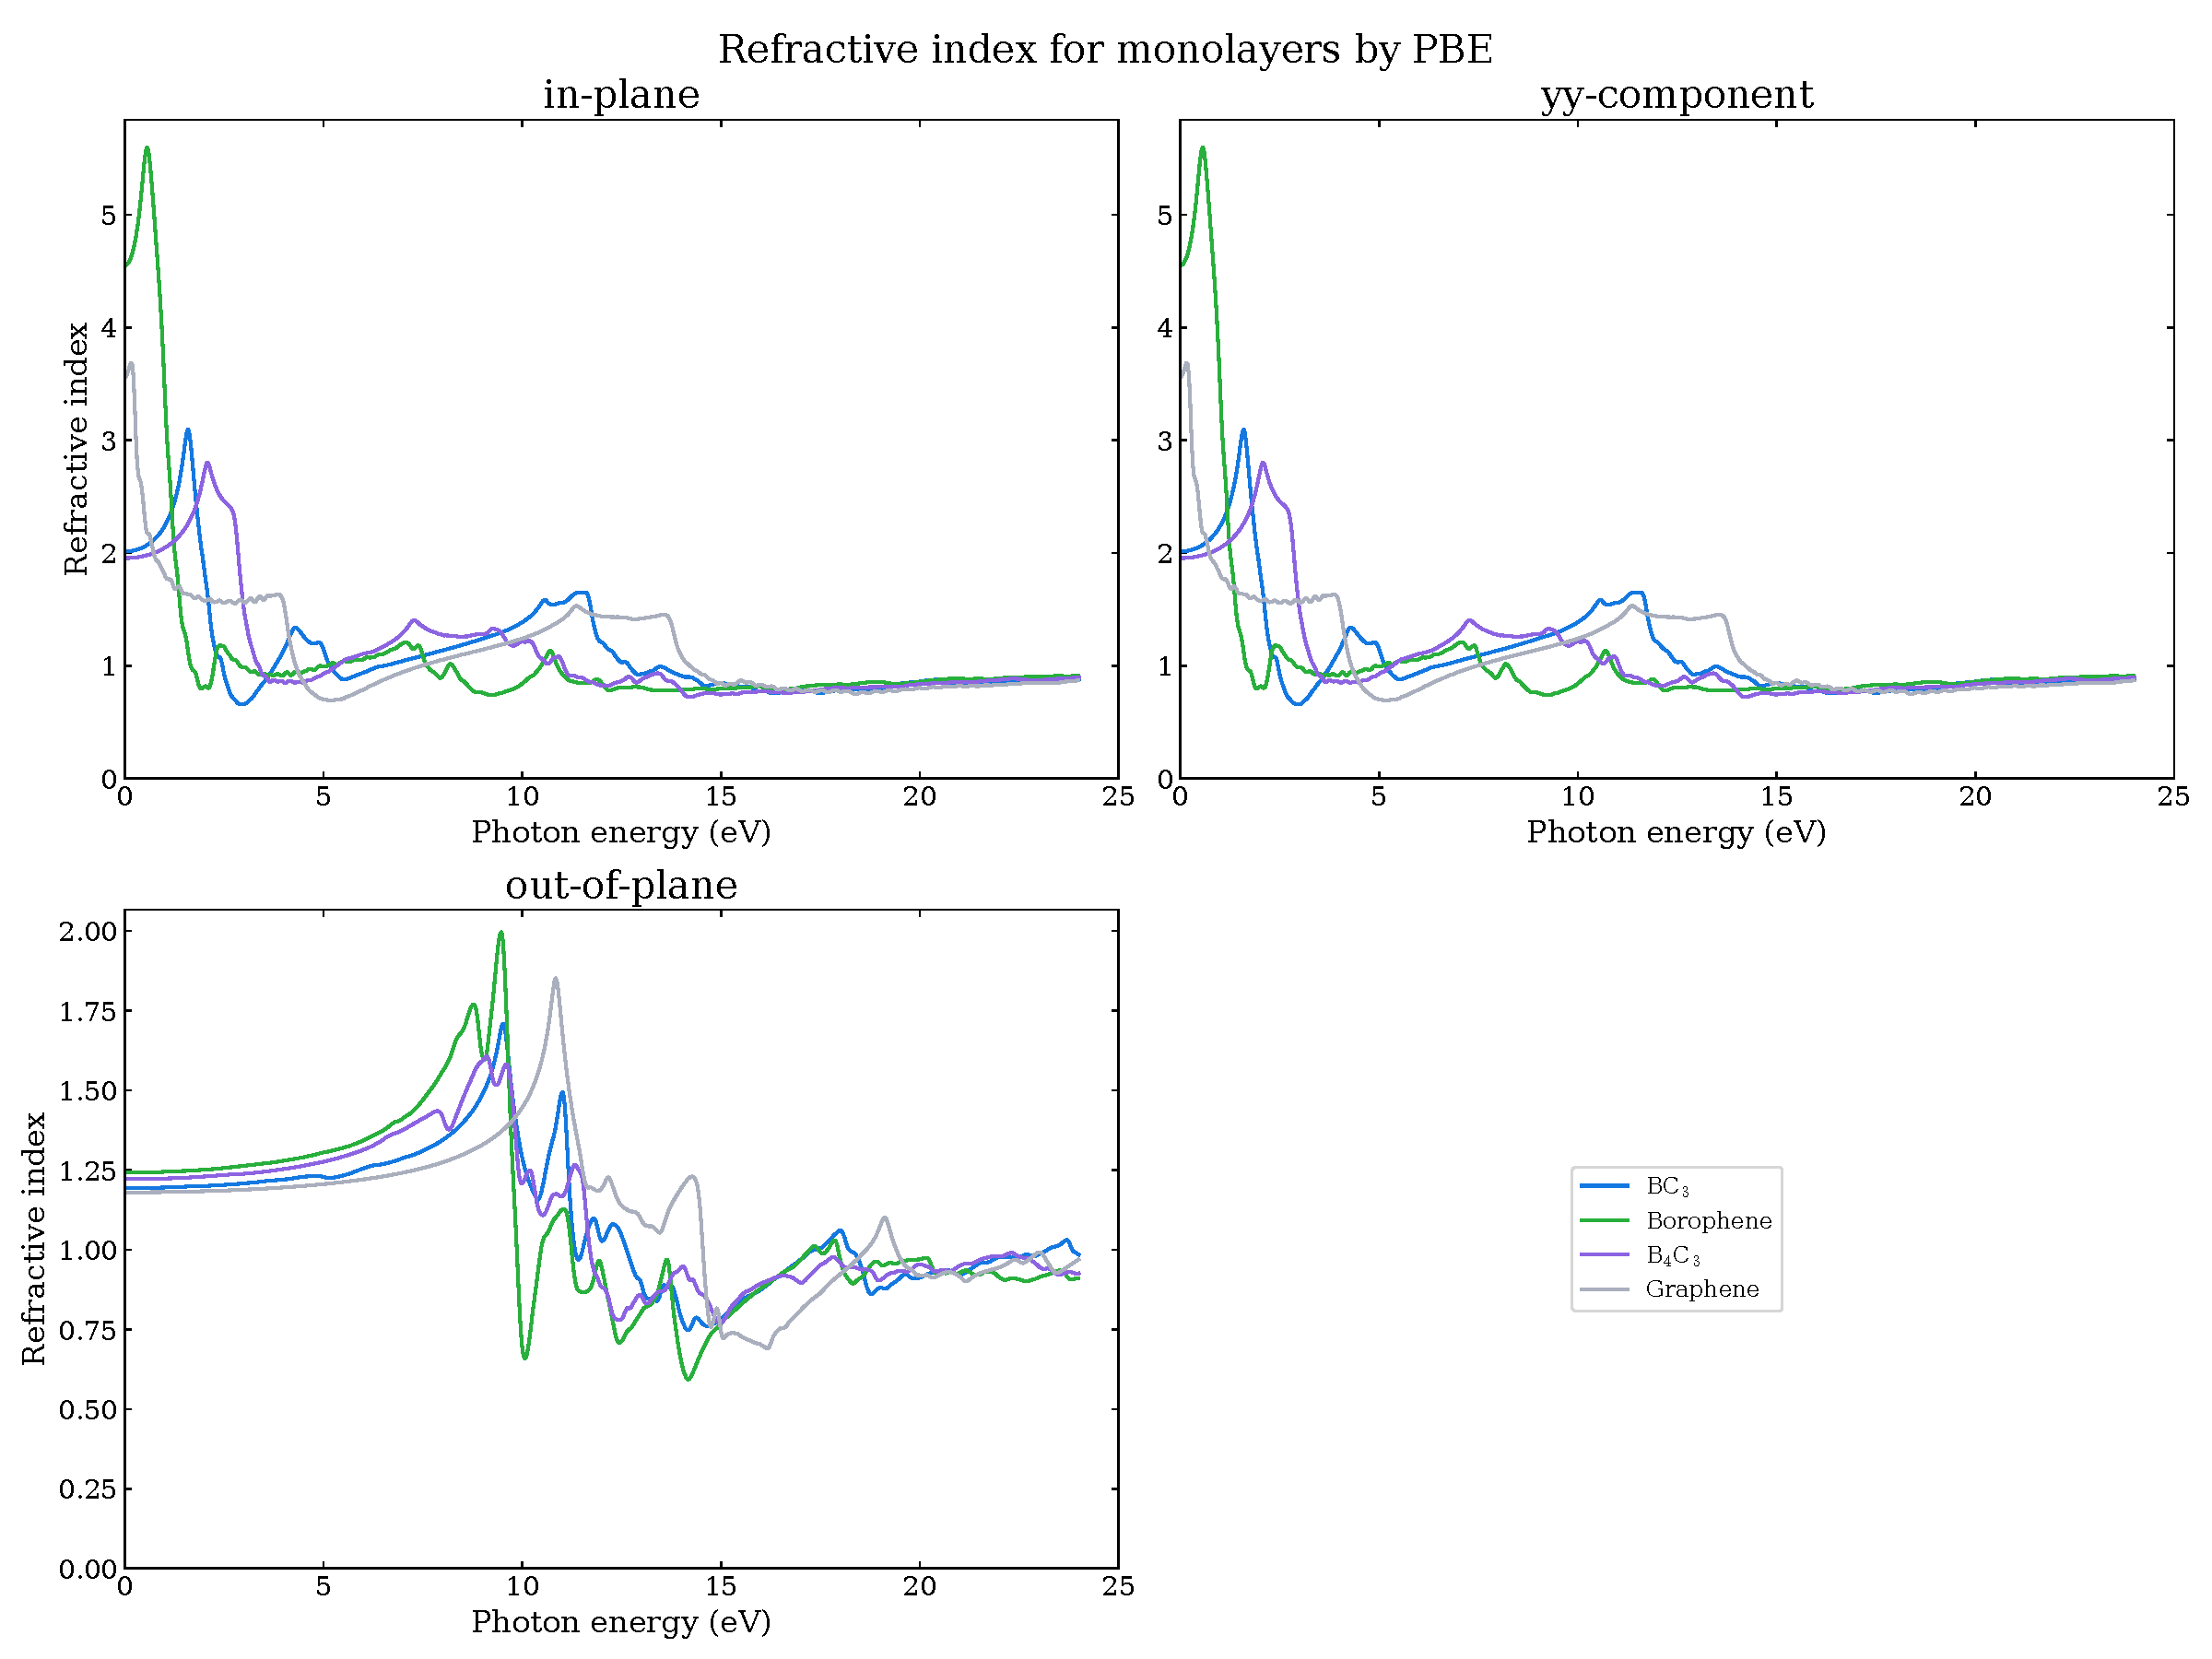
\includegraphics[width=0.80\textwidth]{figures_proj1/S1.14c.pdf}
    \par\nointerlineskip
    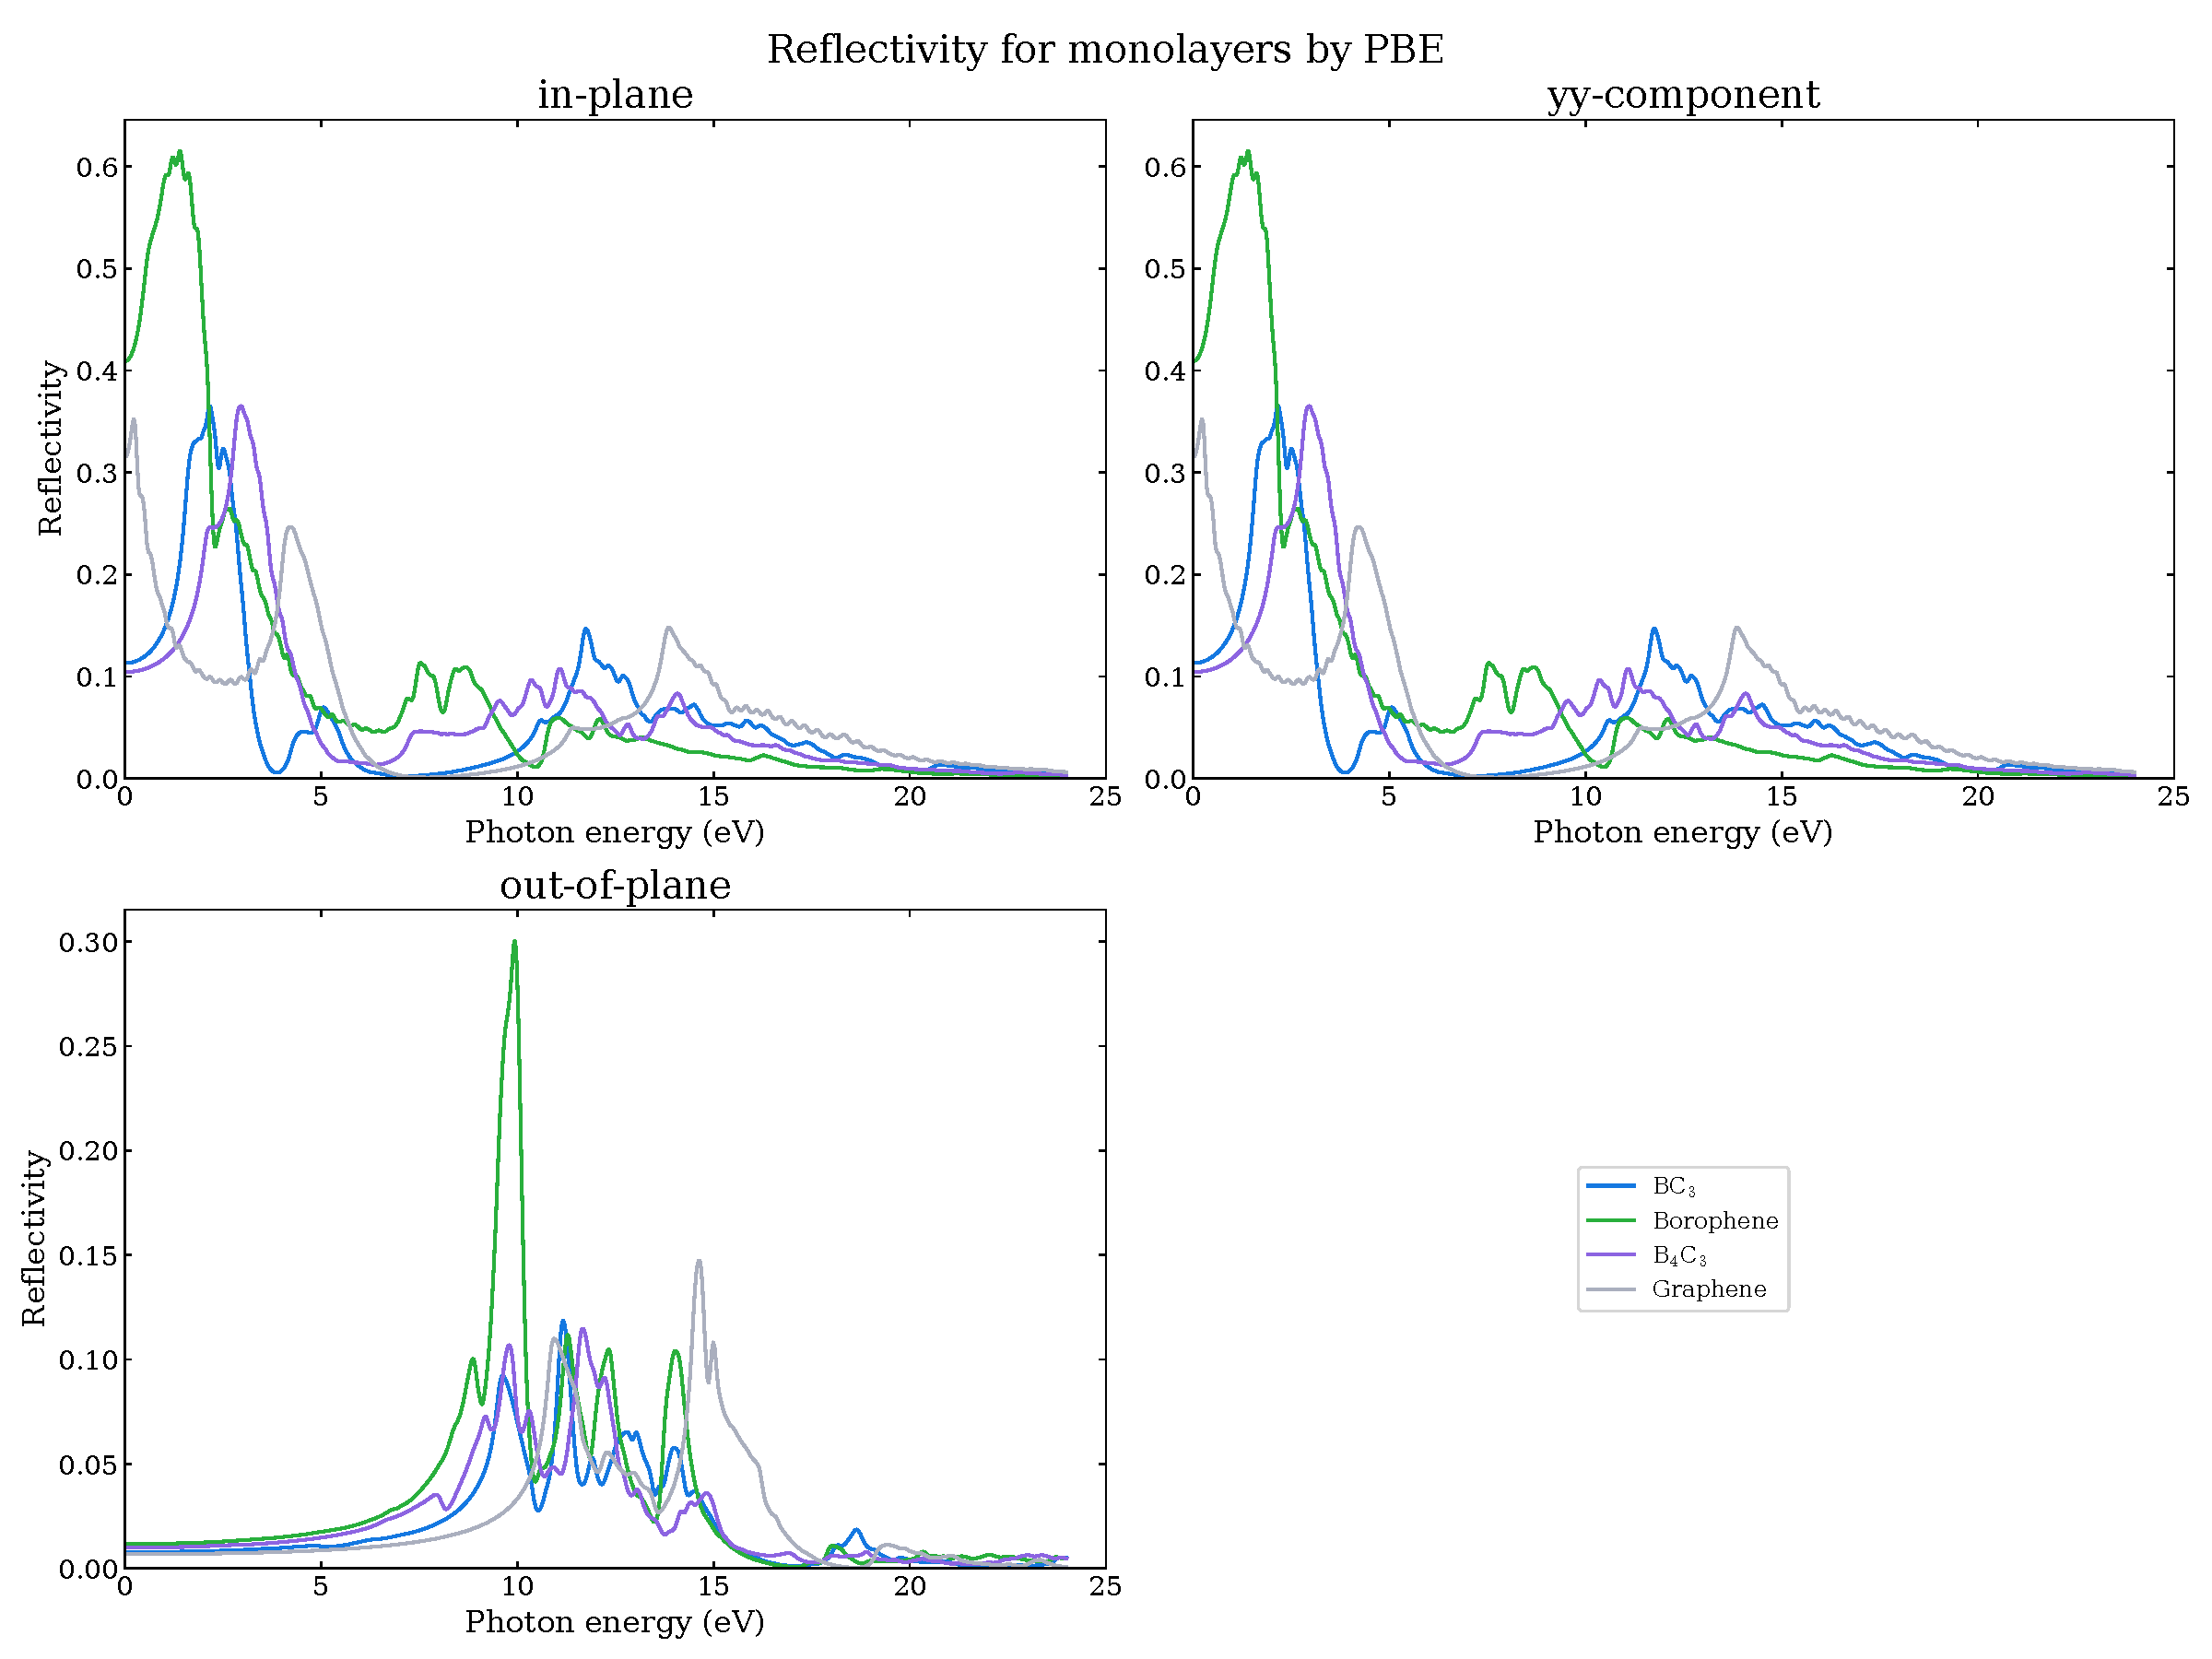
\includegraphics[width=0.80\textwidth]{figures_proj1/S1.14d_correct.pdf}
\caption[]{Optical properties of the four monolayers calculated using PBE (continued).
Upper: Refractive index; lower: Reflectivity.}
\end{figure}

\begin{figure}[!htbp]
\ContinuedFloat
\centering
    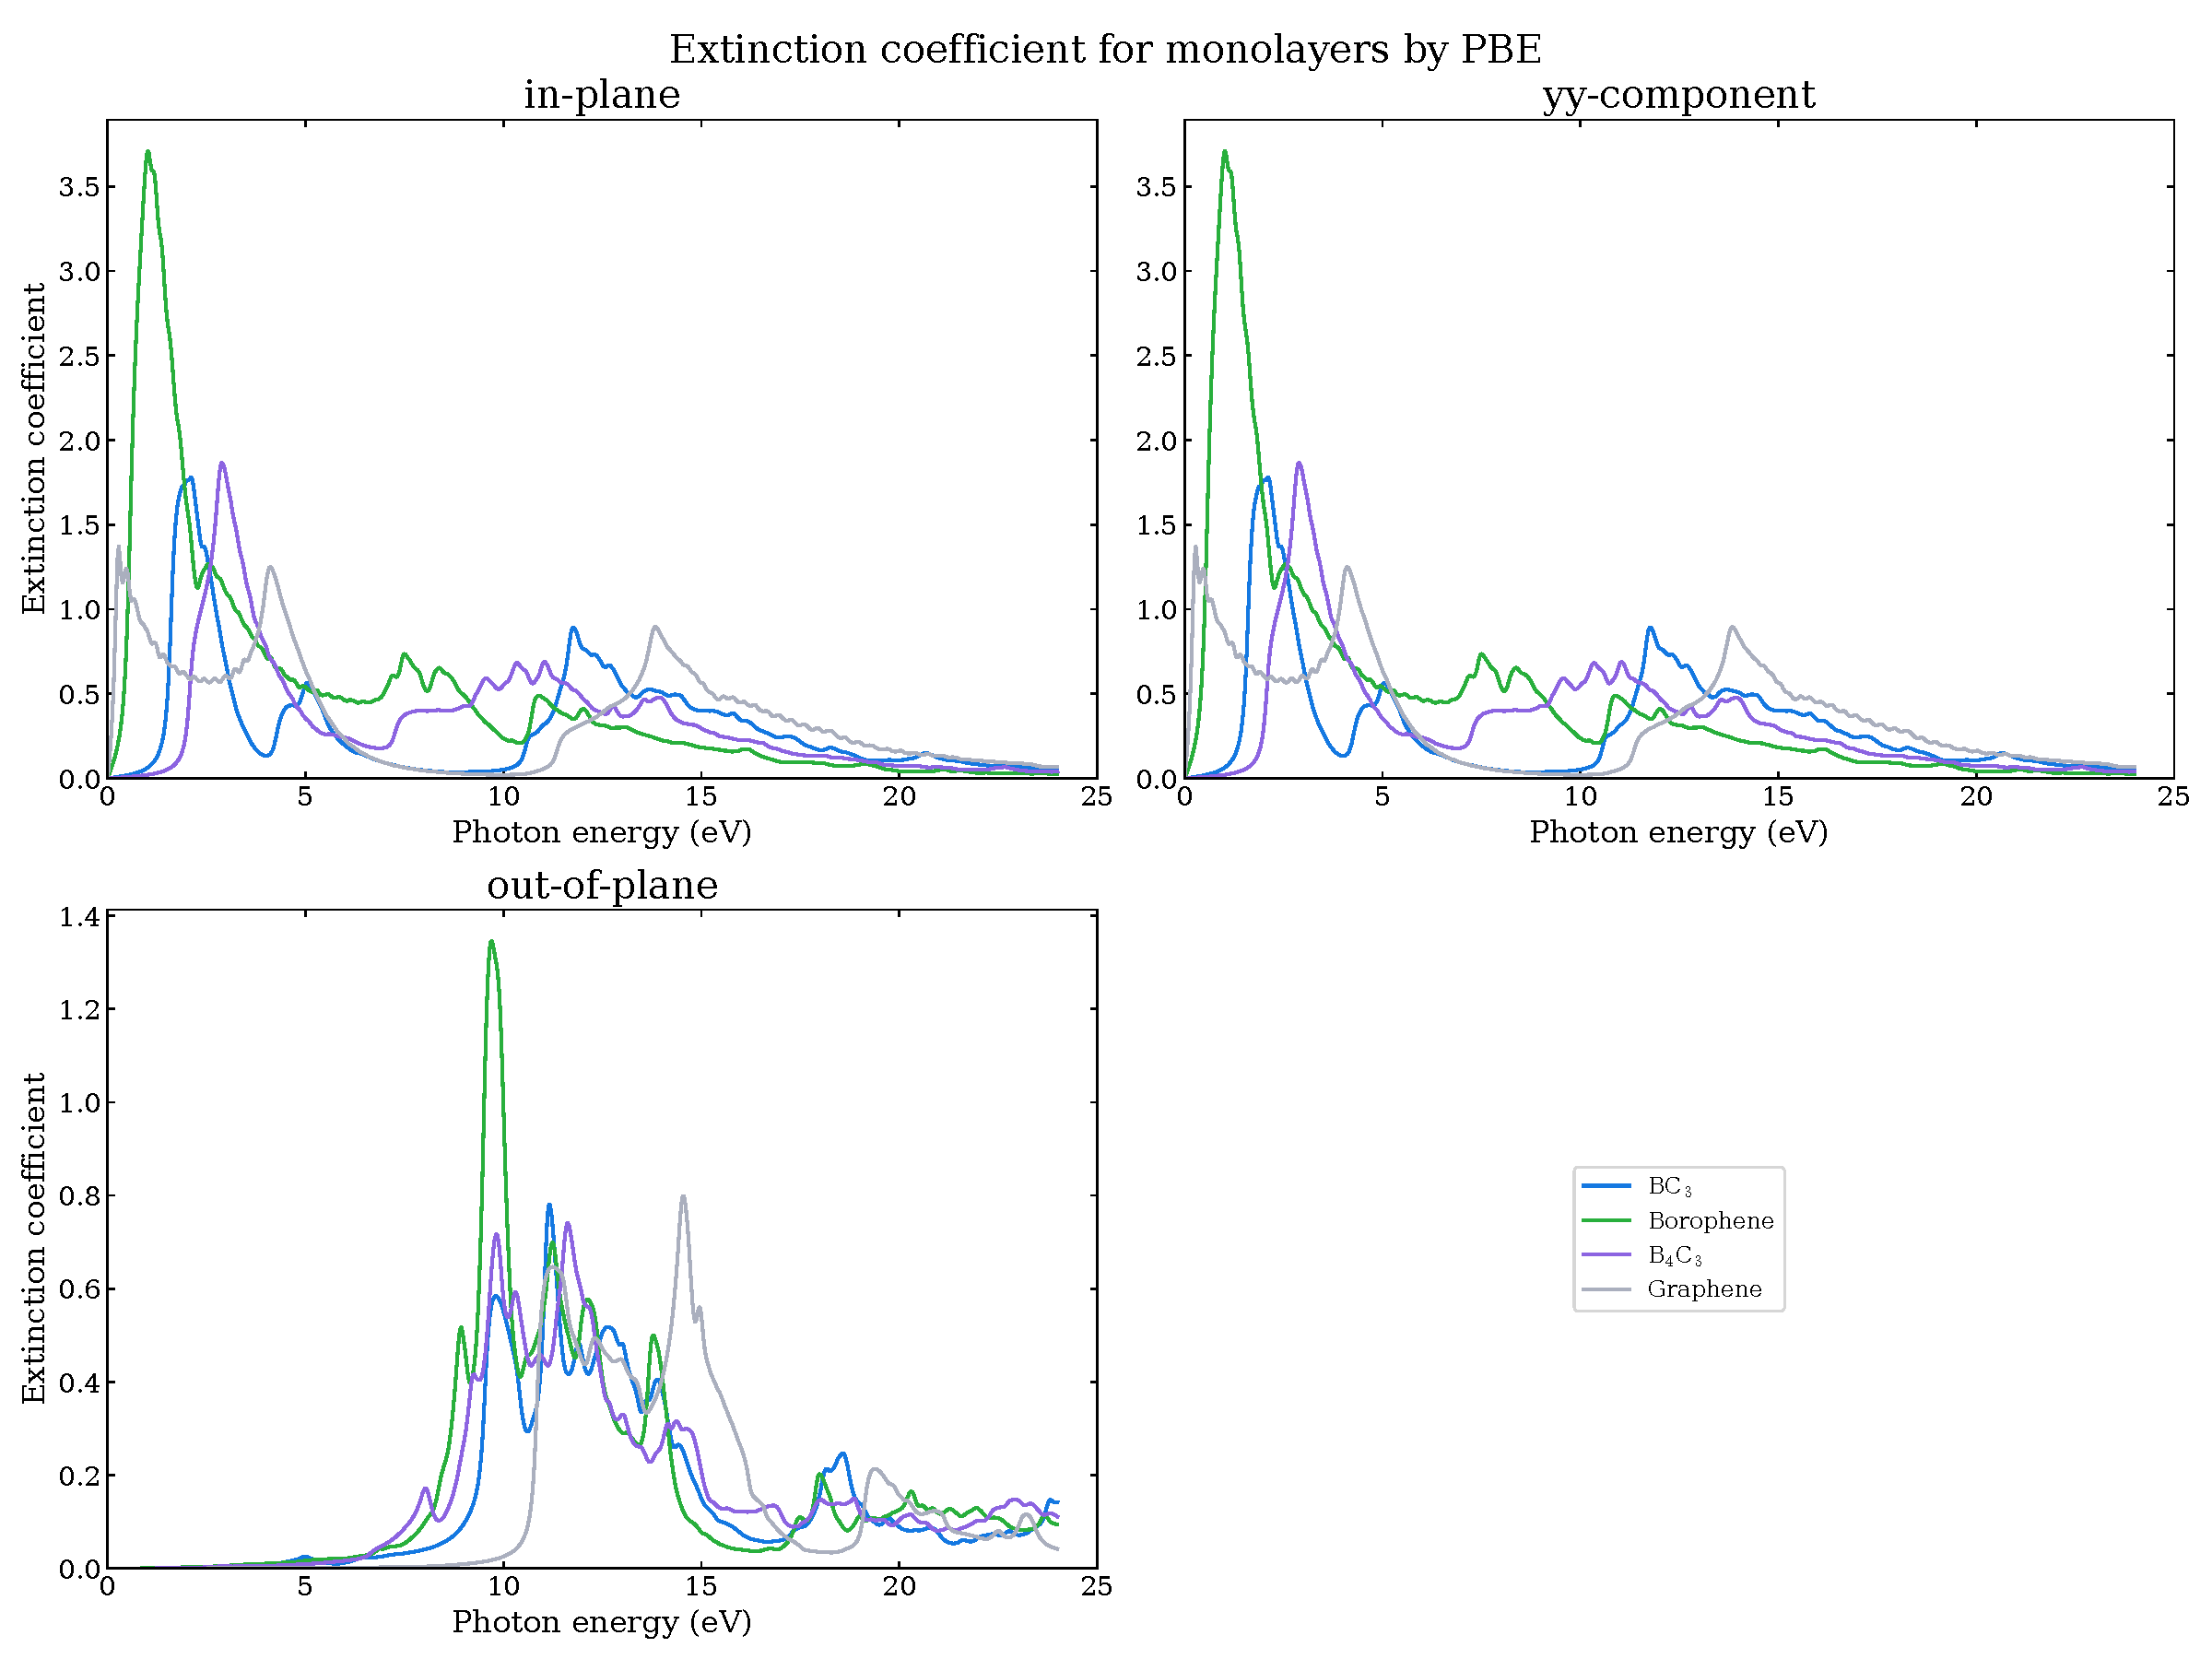
\includegraphics[width=0.80\textwidth]{figures_proj1/S1.14e_correct.pdf}
\caption[]{Optical properties of the four monolayers calculated using PBE (continued): Extinction coefficient.}
\end{figure}

\begin{figure}[!htbp]
\centering
    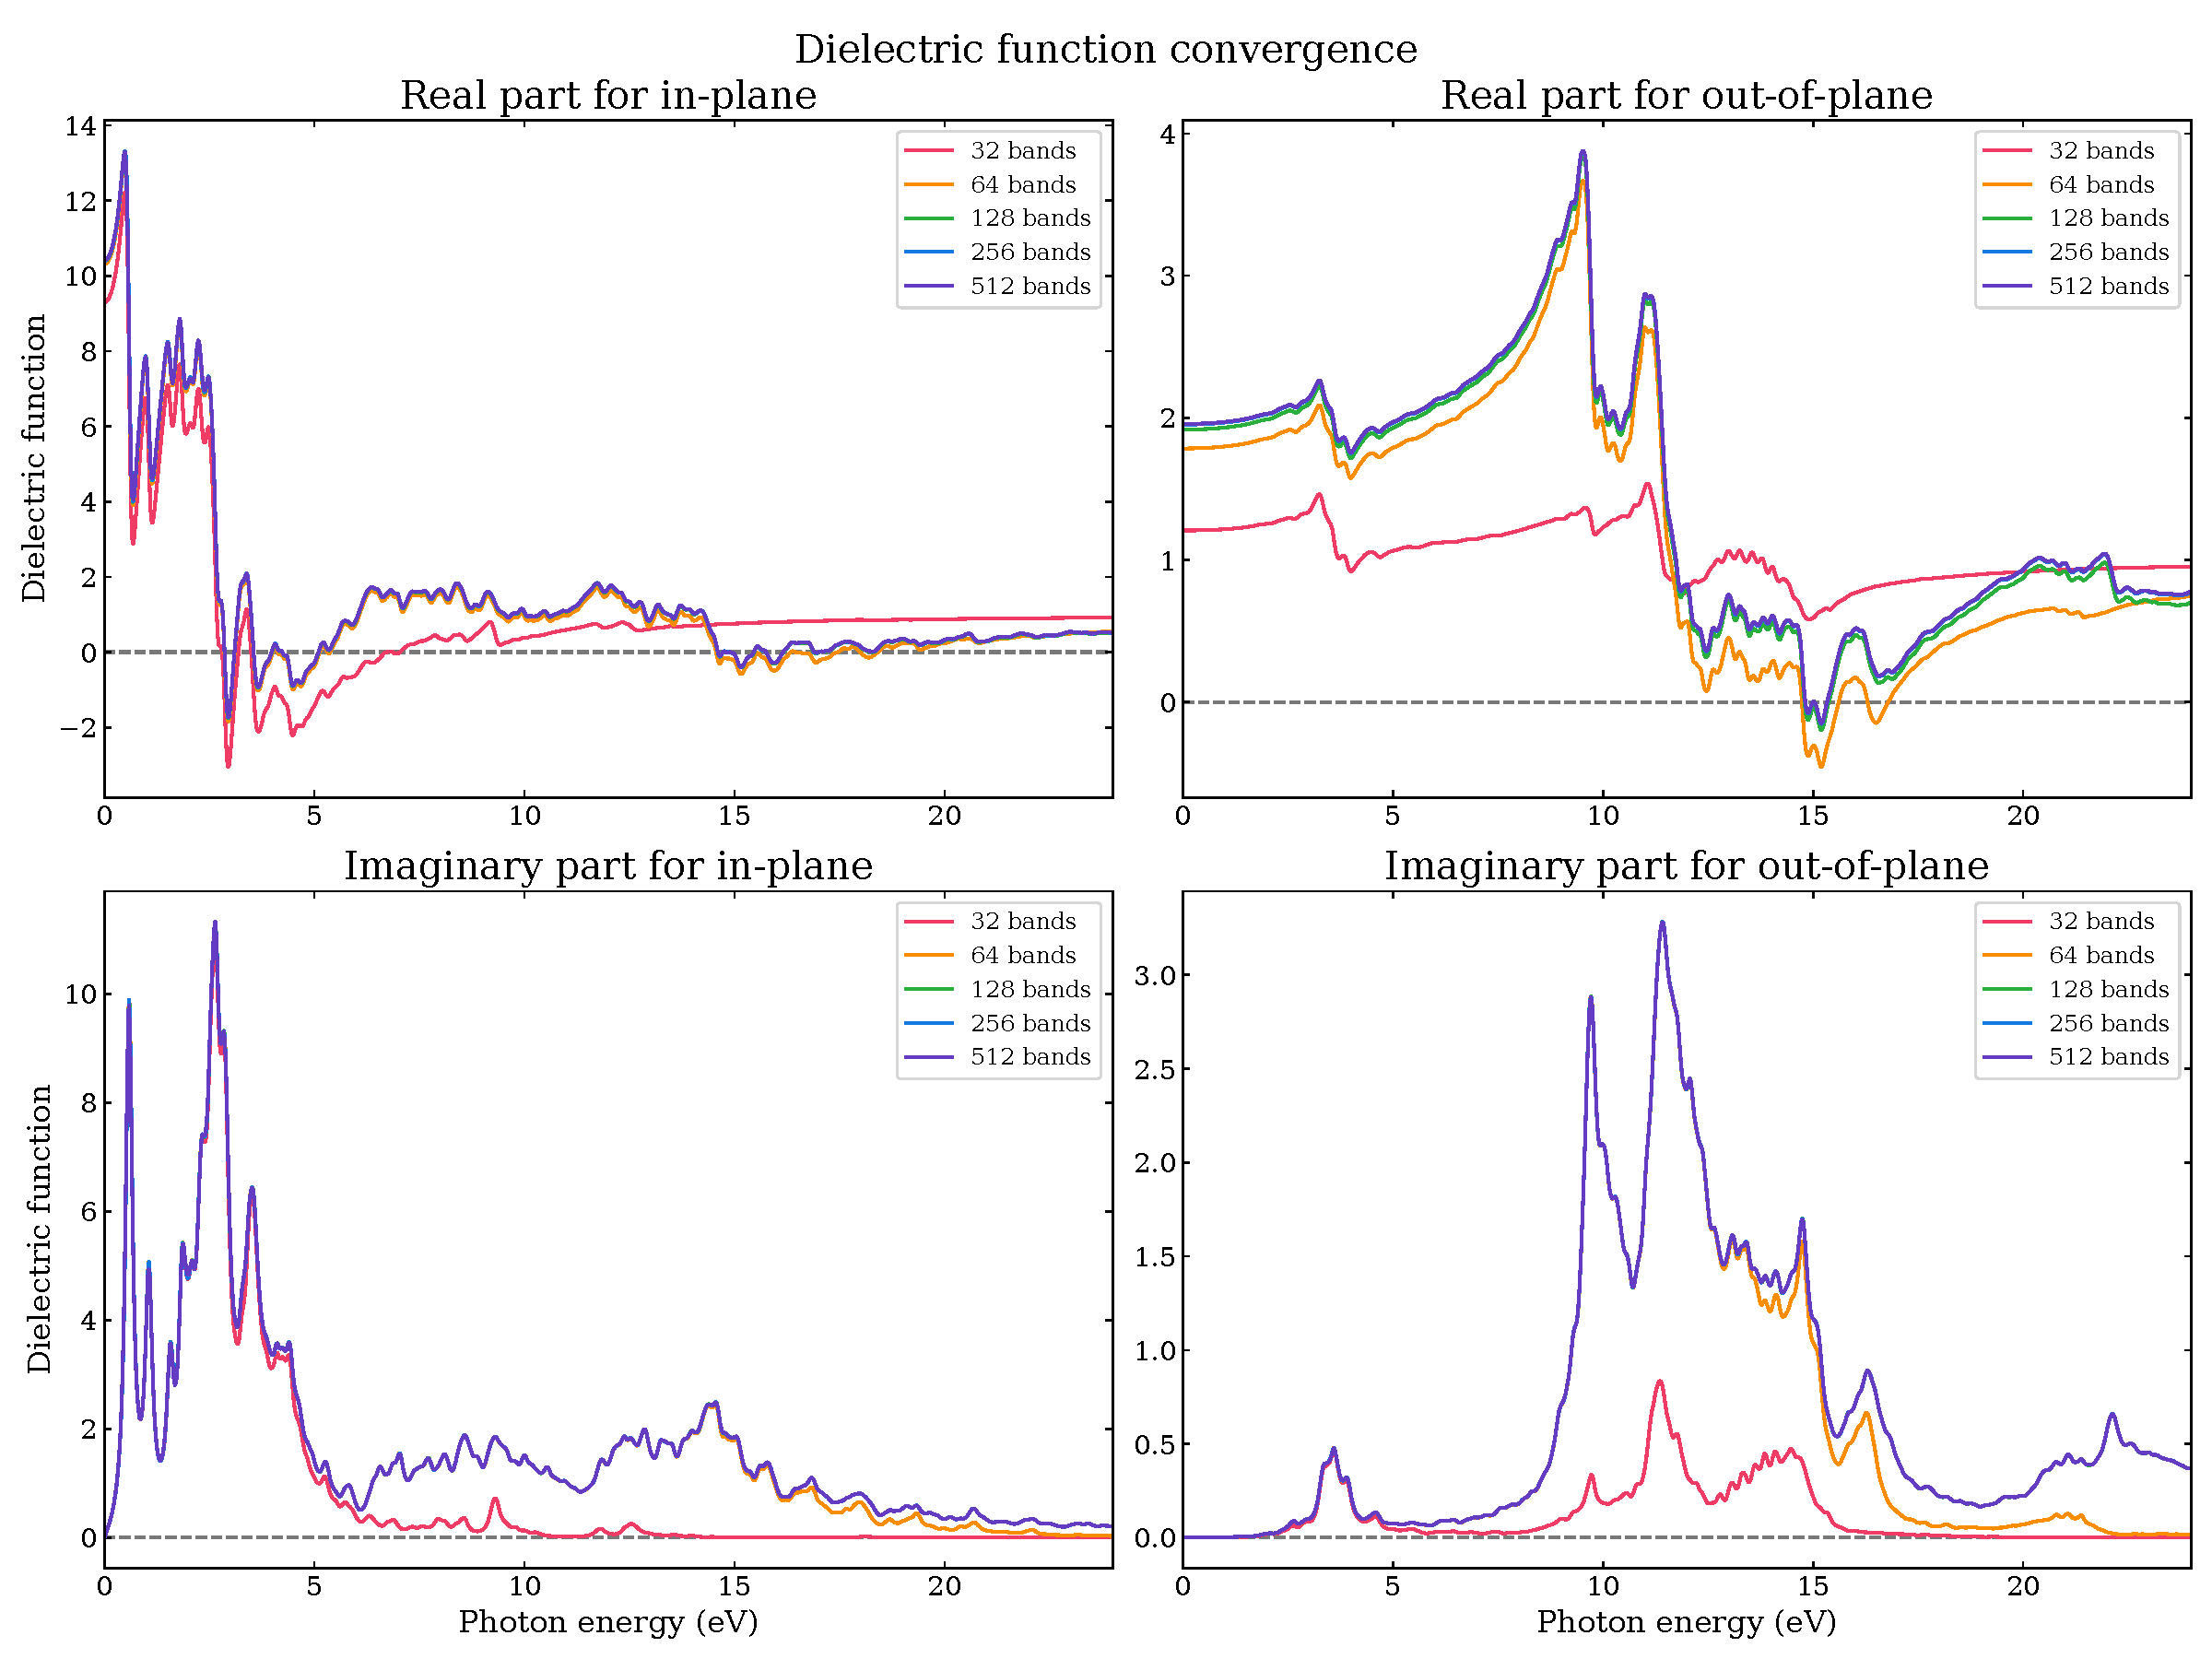
\includegraphics[width=0.80\textwidth]{figures_proj1/S1.15.pdf}
\caption{Convergence test of the dielectric function of Graphene-\ce{B4C3} with respect to the total number of bands, including unoccupied states, calculated using PBE.}
\label{S1.15}
\end{figure}

Figure~\ref{S1.16} also shows the effect of the energy convergence criterion \texttt{EDIFF} on the calculated dielectric function, together with the effects of different k-point meshes and the comparison between HSE06 and PBE.

\begin{figure}[!htbp]
\centering
    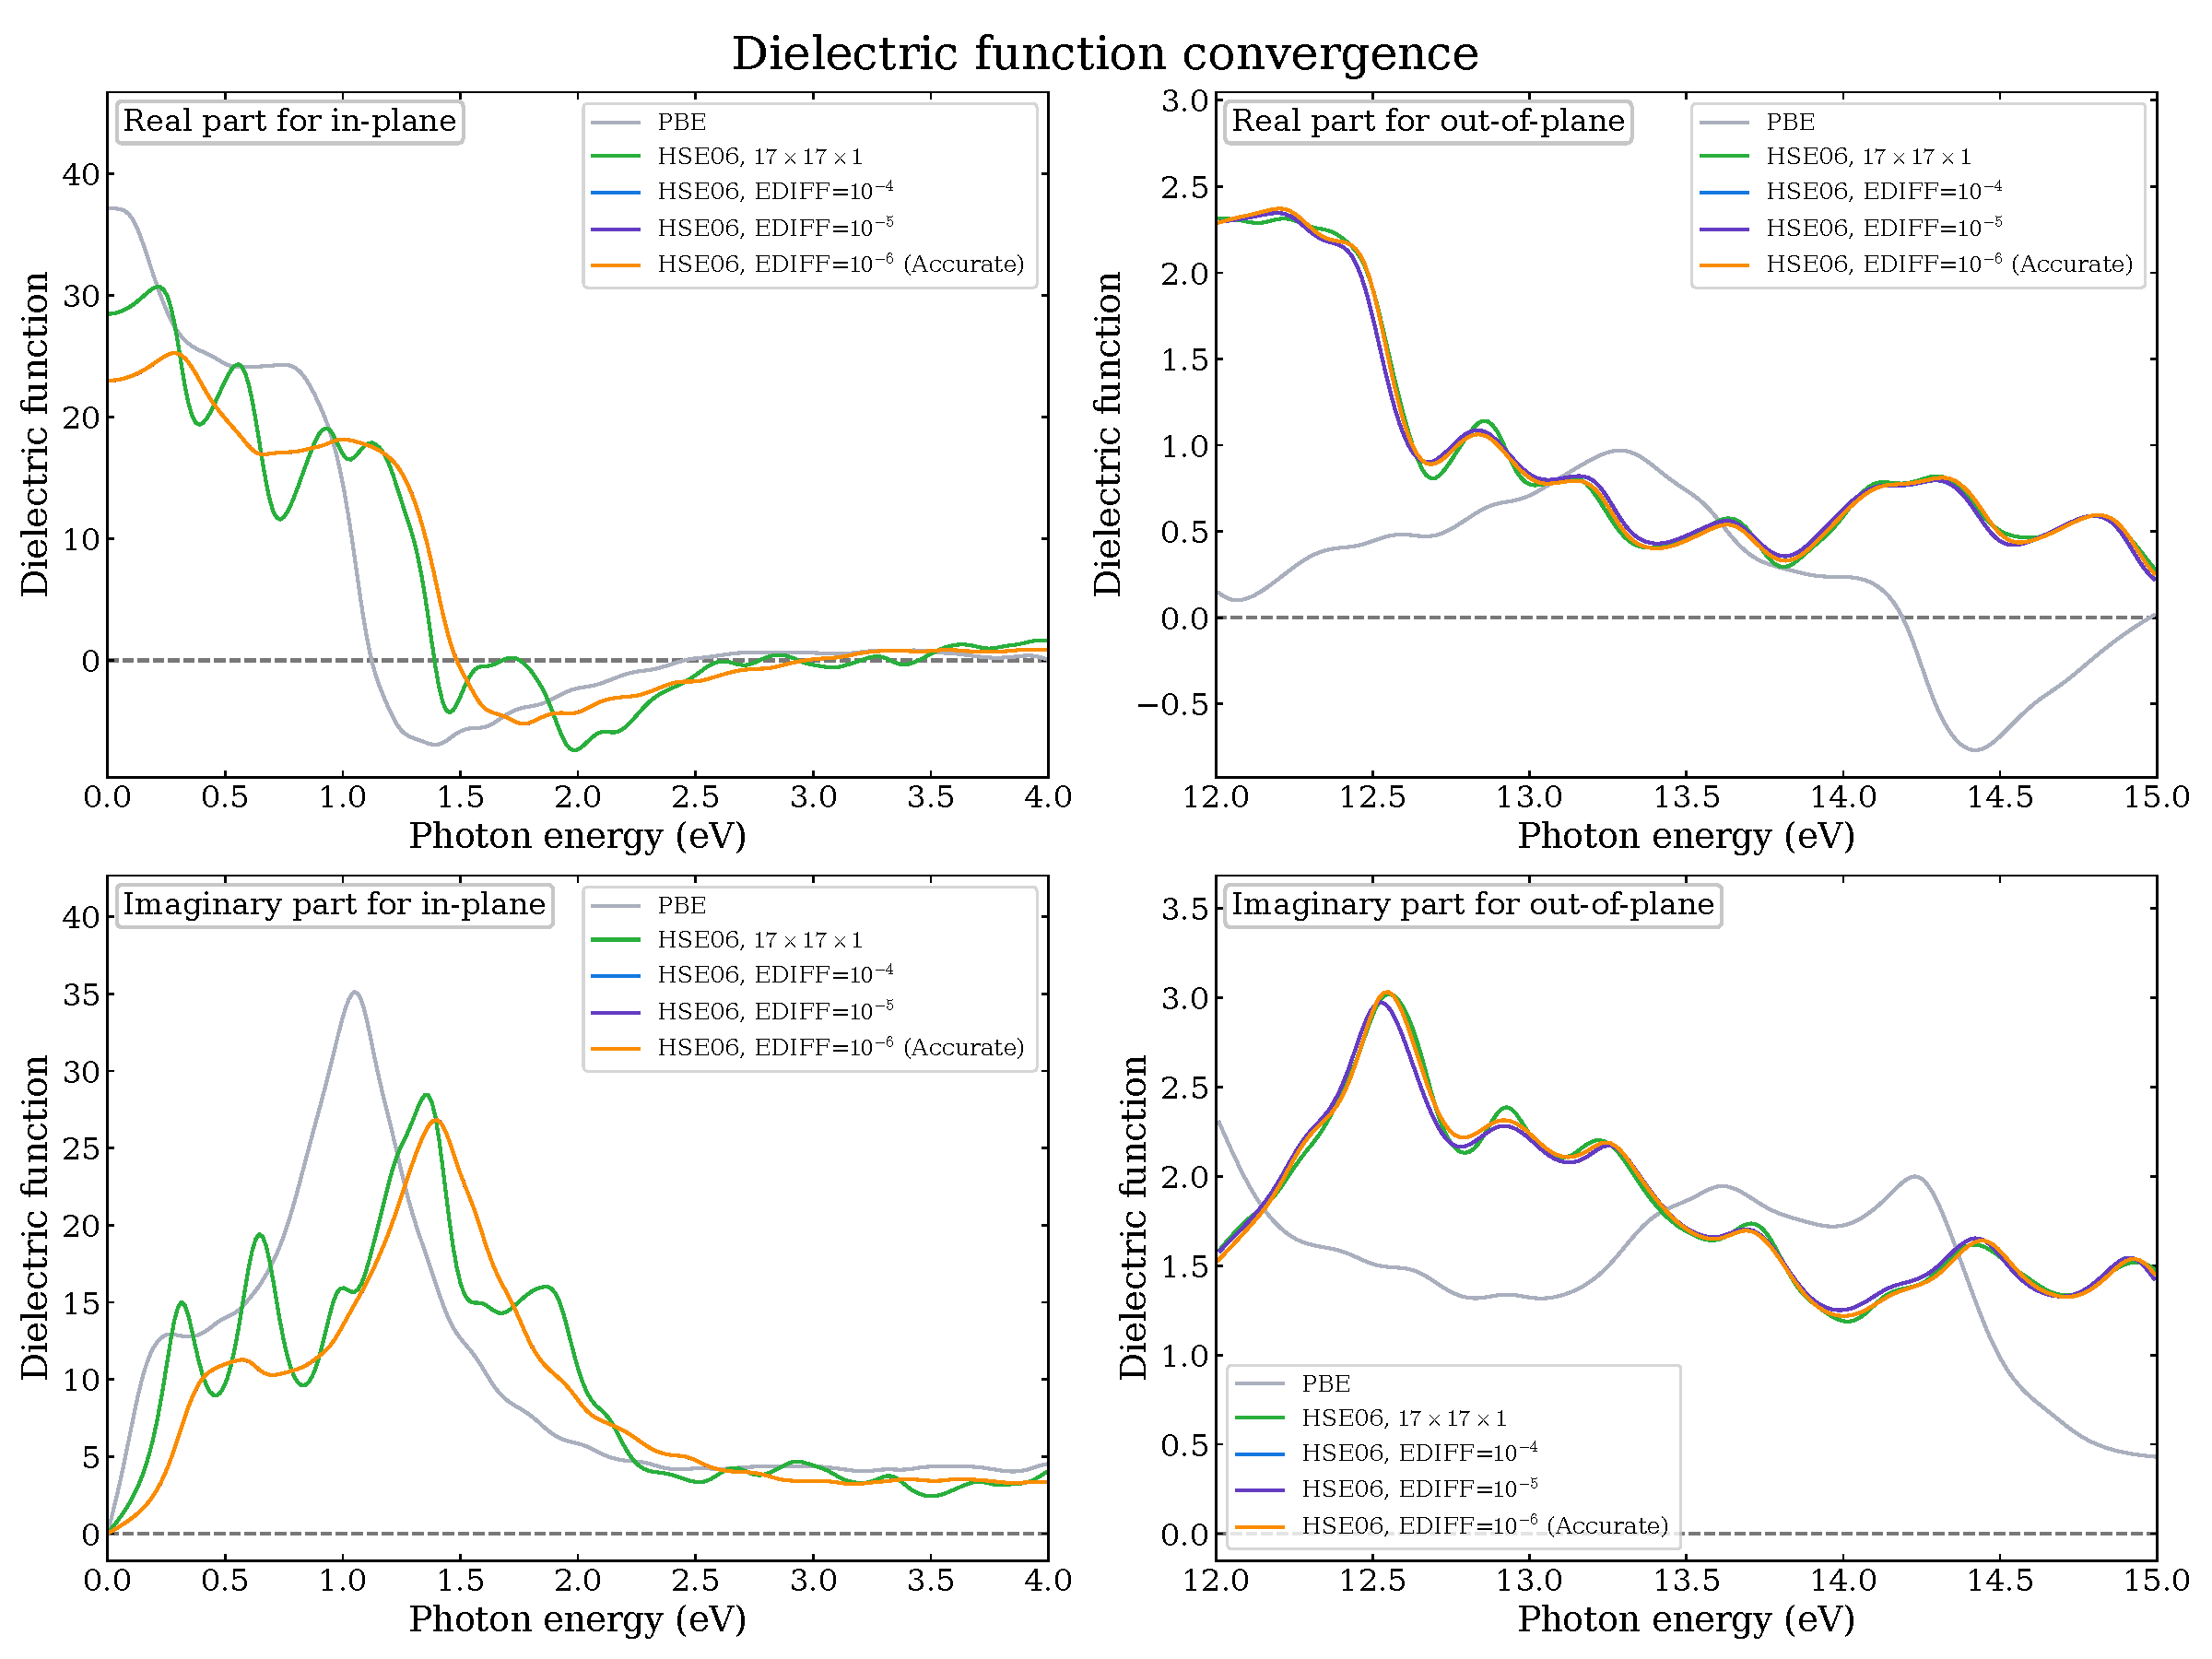
\includegraphics[width=0.80\textwidth]{figures_proj1/S1.16_alt.pdf}
\caption[Dielectric-function convergence tests for the Graphene-Borophene bilayer.]{Dielectric function of the Graphene-Borophene bilayer comparing PBE and HSE06 results, HSE06 k-point meshes of $17 \times 17 \times 1$ and $65 \times 65 \times 1$, and HSE06 energy convergence criteria \texttt{EDIFF} = $10^{-4}$, $10^{-5}$, and $10^{-6}$.
The $10^{-4}$ and $10^{-5}$ calculations use \texttt{PREC=Normal}, while the $10^{-6}$ calculation uses \texttt{PREC=Accurate}.}
\label{S1.16}
\end{figure}

Figures~\ref{S1.17}--\ref{S1.19} show the full dielectric-function tensor components of the three bilayer systems,
as calculated using both the PBE and HSE06 functionals.
The diagonal components describe the dominant in-plane and out-of-plane optical responses,
whereas the off-diagonal components describe the coupling between different Cartesian directions.
The displayed off-diagonal components are negligible for Graphene-Borophene,
but remain finite for Graphene-\ce{BC3} and Graphene-\ce{B4C3}.
Their opposite-sign pairs cancel in the symmetric tensor of the reciprocal response.

In addition, figures~\ref{S1.20}--\ref{S1.24} compare the optical properties derived from the diagonal HSE06 dielectric components for the three bilayer heterostructures.
These properties include the absorption coefficient, energy-loss spectrum, refractive index, reflectivity, and extinction coefficient.
The $xx$ and $yy$ components correspond to electric-field polarizations within the layers,
whereas $zz$ corresponds to polarization perpendicular to the layers.
The diagonal results below use the principal-axis description, which applies to the symmetric tensors of all three systems.

\begin{figure}[!htbp]
\centering
    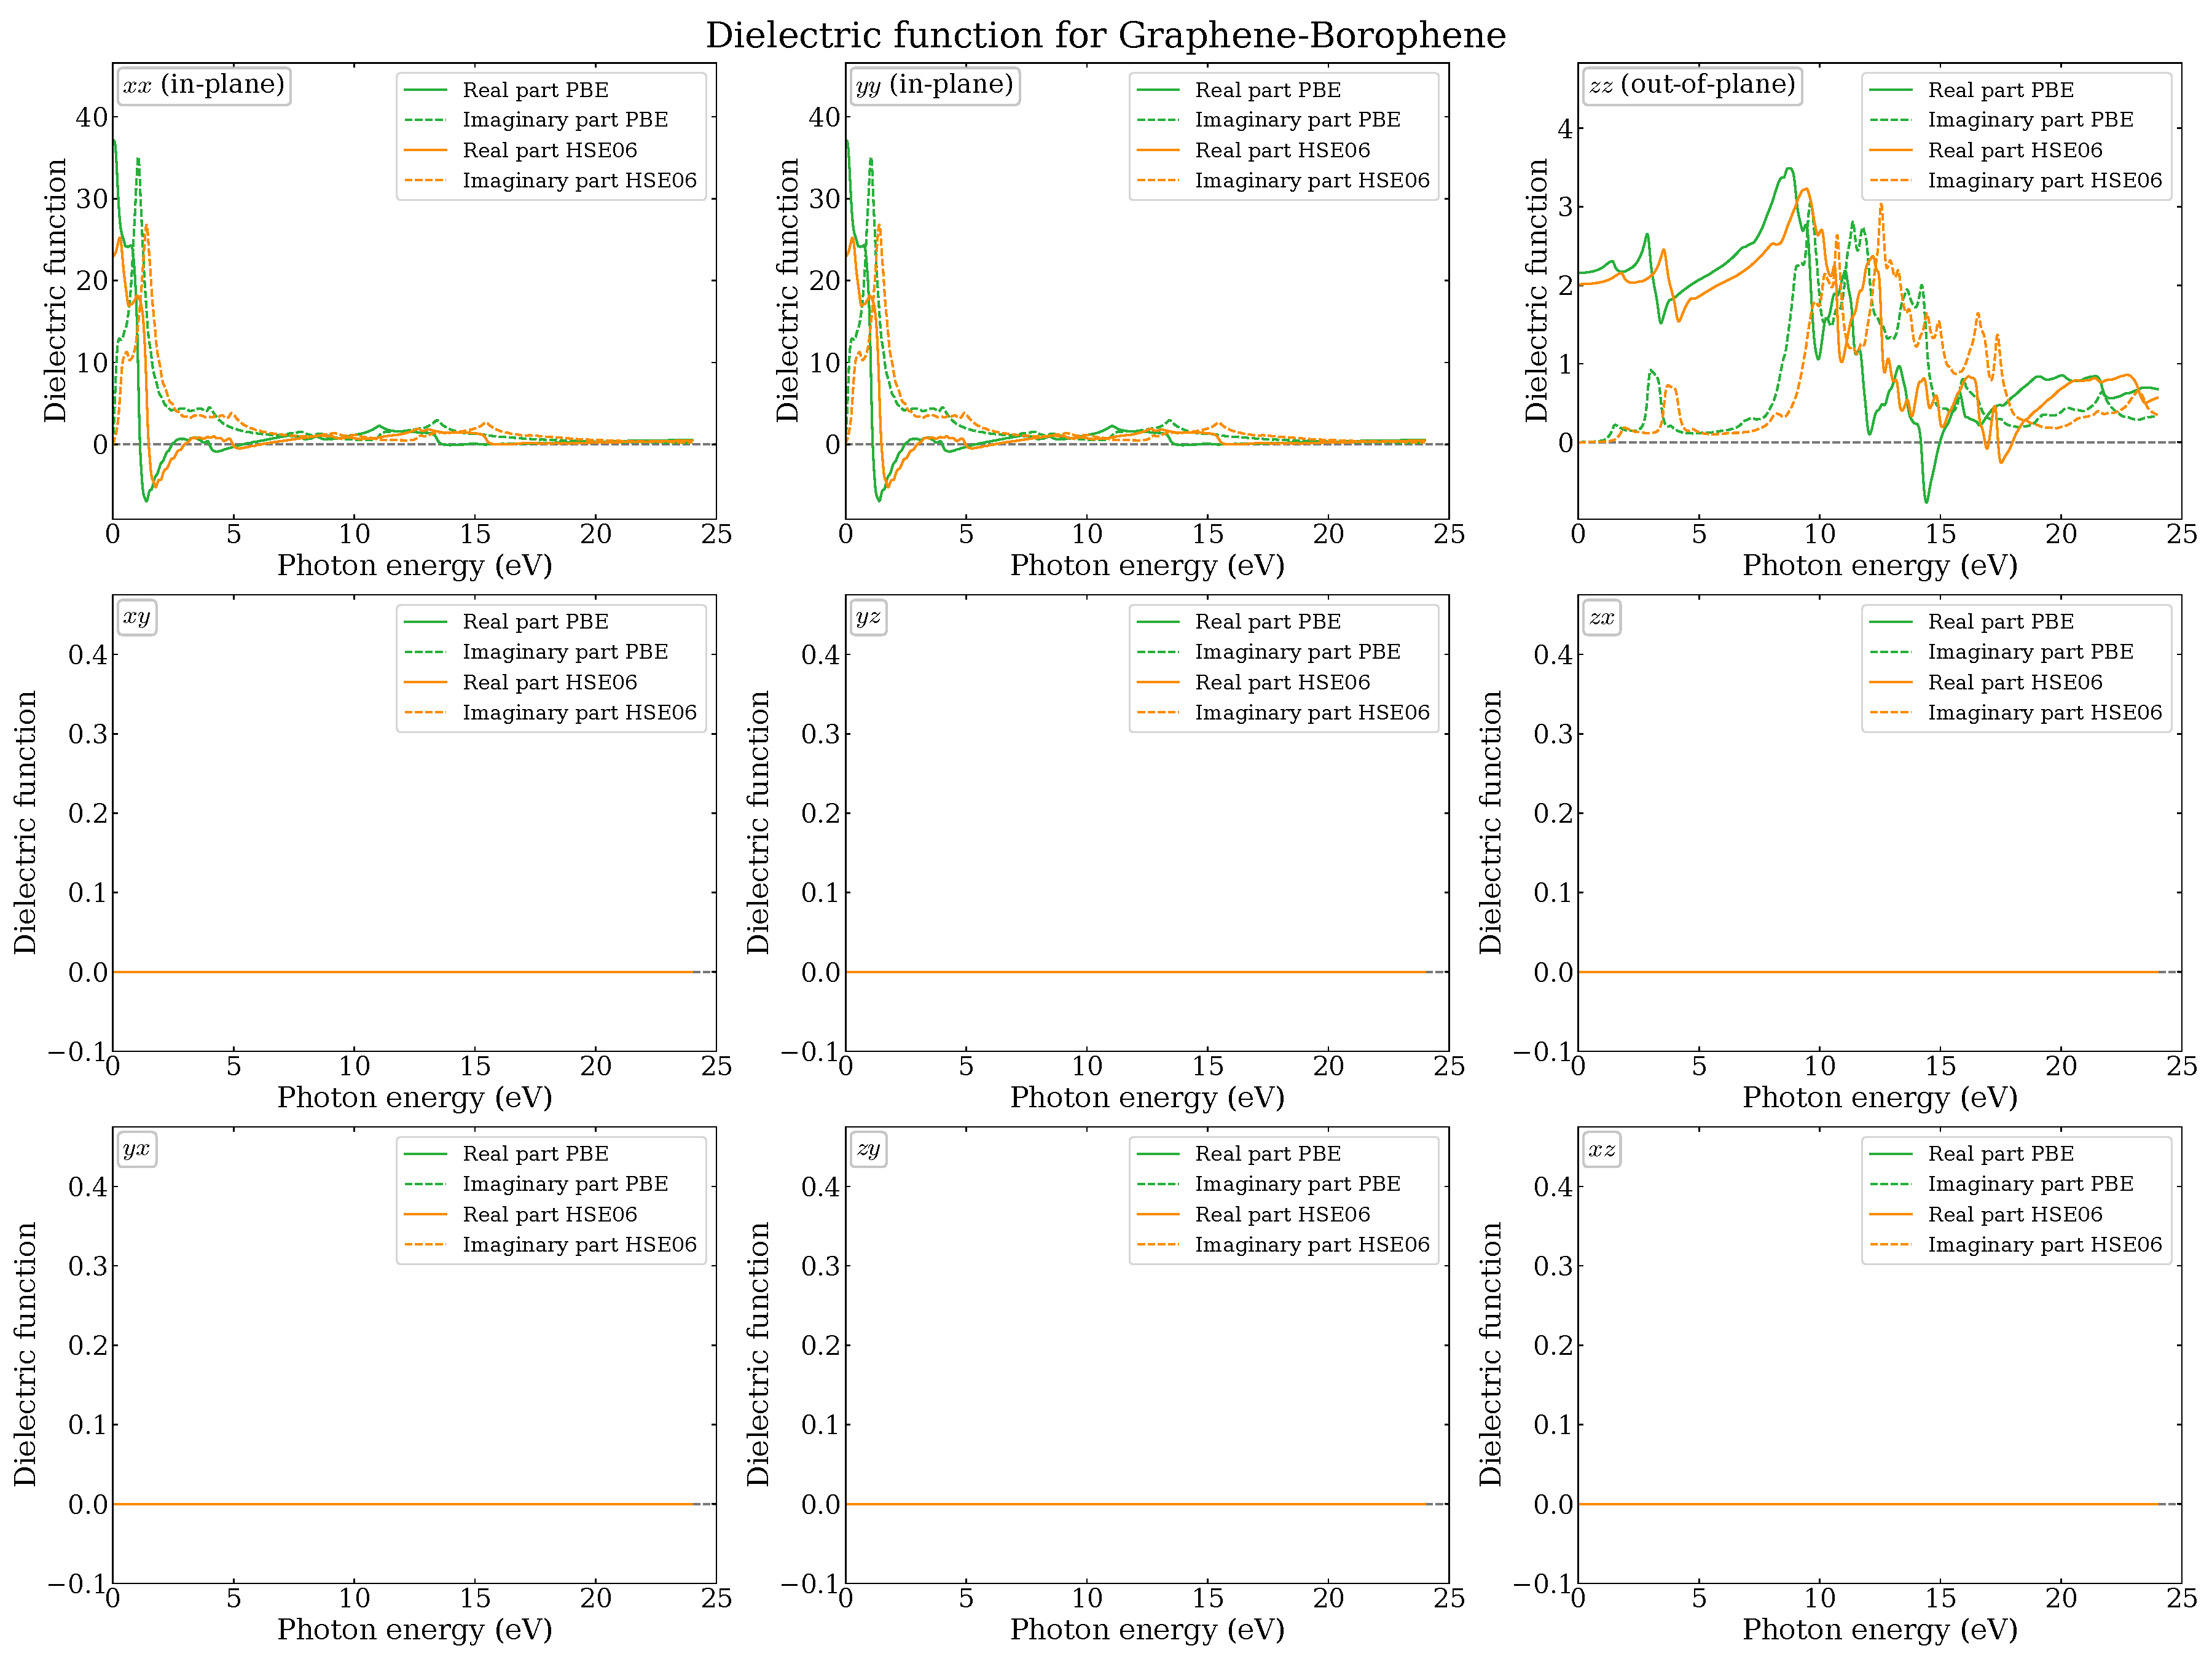
\includegraphics[width=1.00\textwidth]{figures_proj1/S1.17_alt.pdf}
\caption[Dielectric tensor of Graphene-Borophene calculated using PBE and HSE06.]{Dimensionless dielectric tensor components of Graphene-Borophene versus photon energy $\hbar\omega$ in \unit{\electronvolt}.
From left to right, the rows show $xx,yy,zz$; $xy,yz,zx$; and $yx,zy,xz$.
The $xx$ and $yy$ directions lie within the layers, while $zz$ is perpendicular to them.
Green and orange curves denote PBE and HSE06, respectively; solid and dashed lines denote real and imaginary parts.
The off-diagonal components are negligible on the plotted scale.}
\label{S1.17}
\end{figure}

\begin{figure}[!htbp]
\centering
    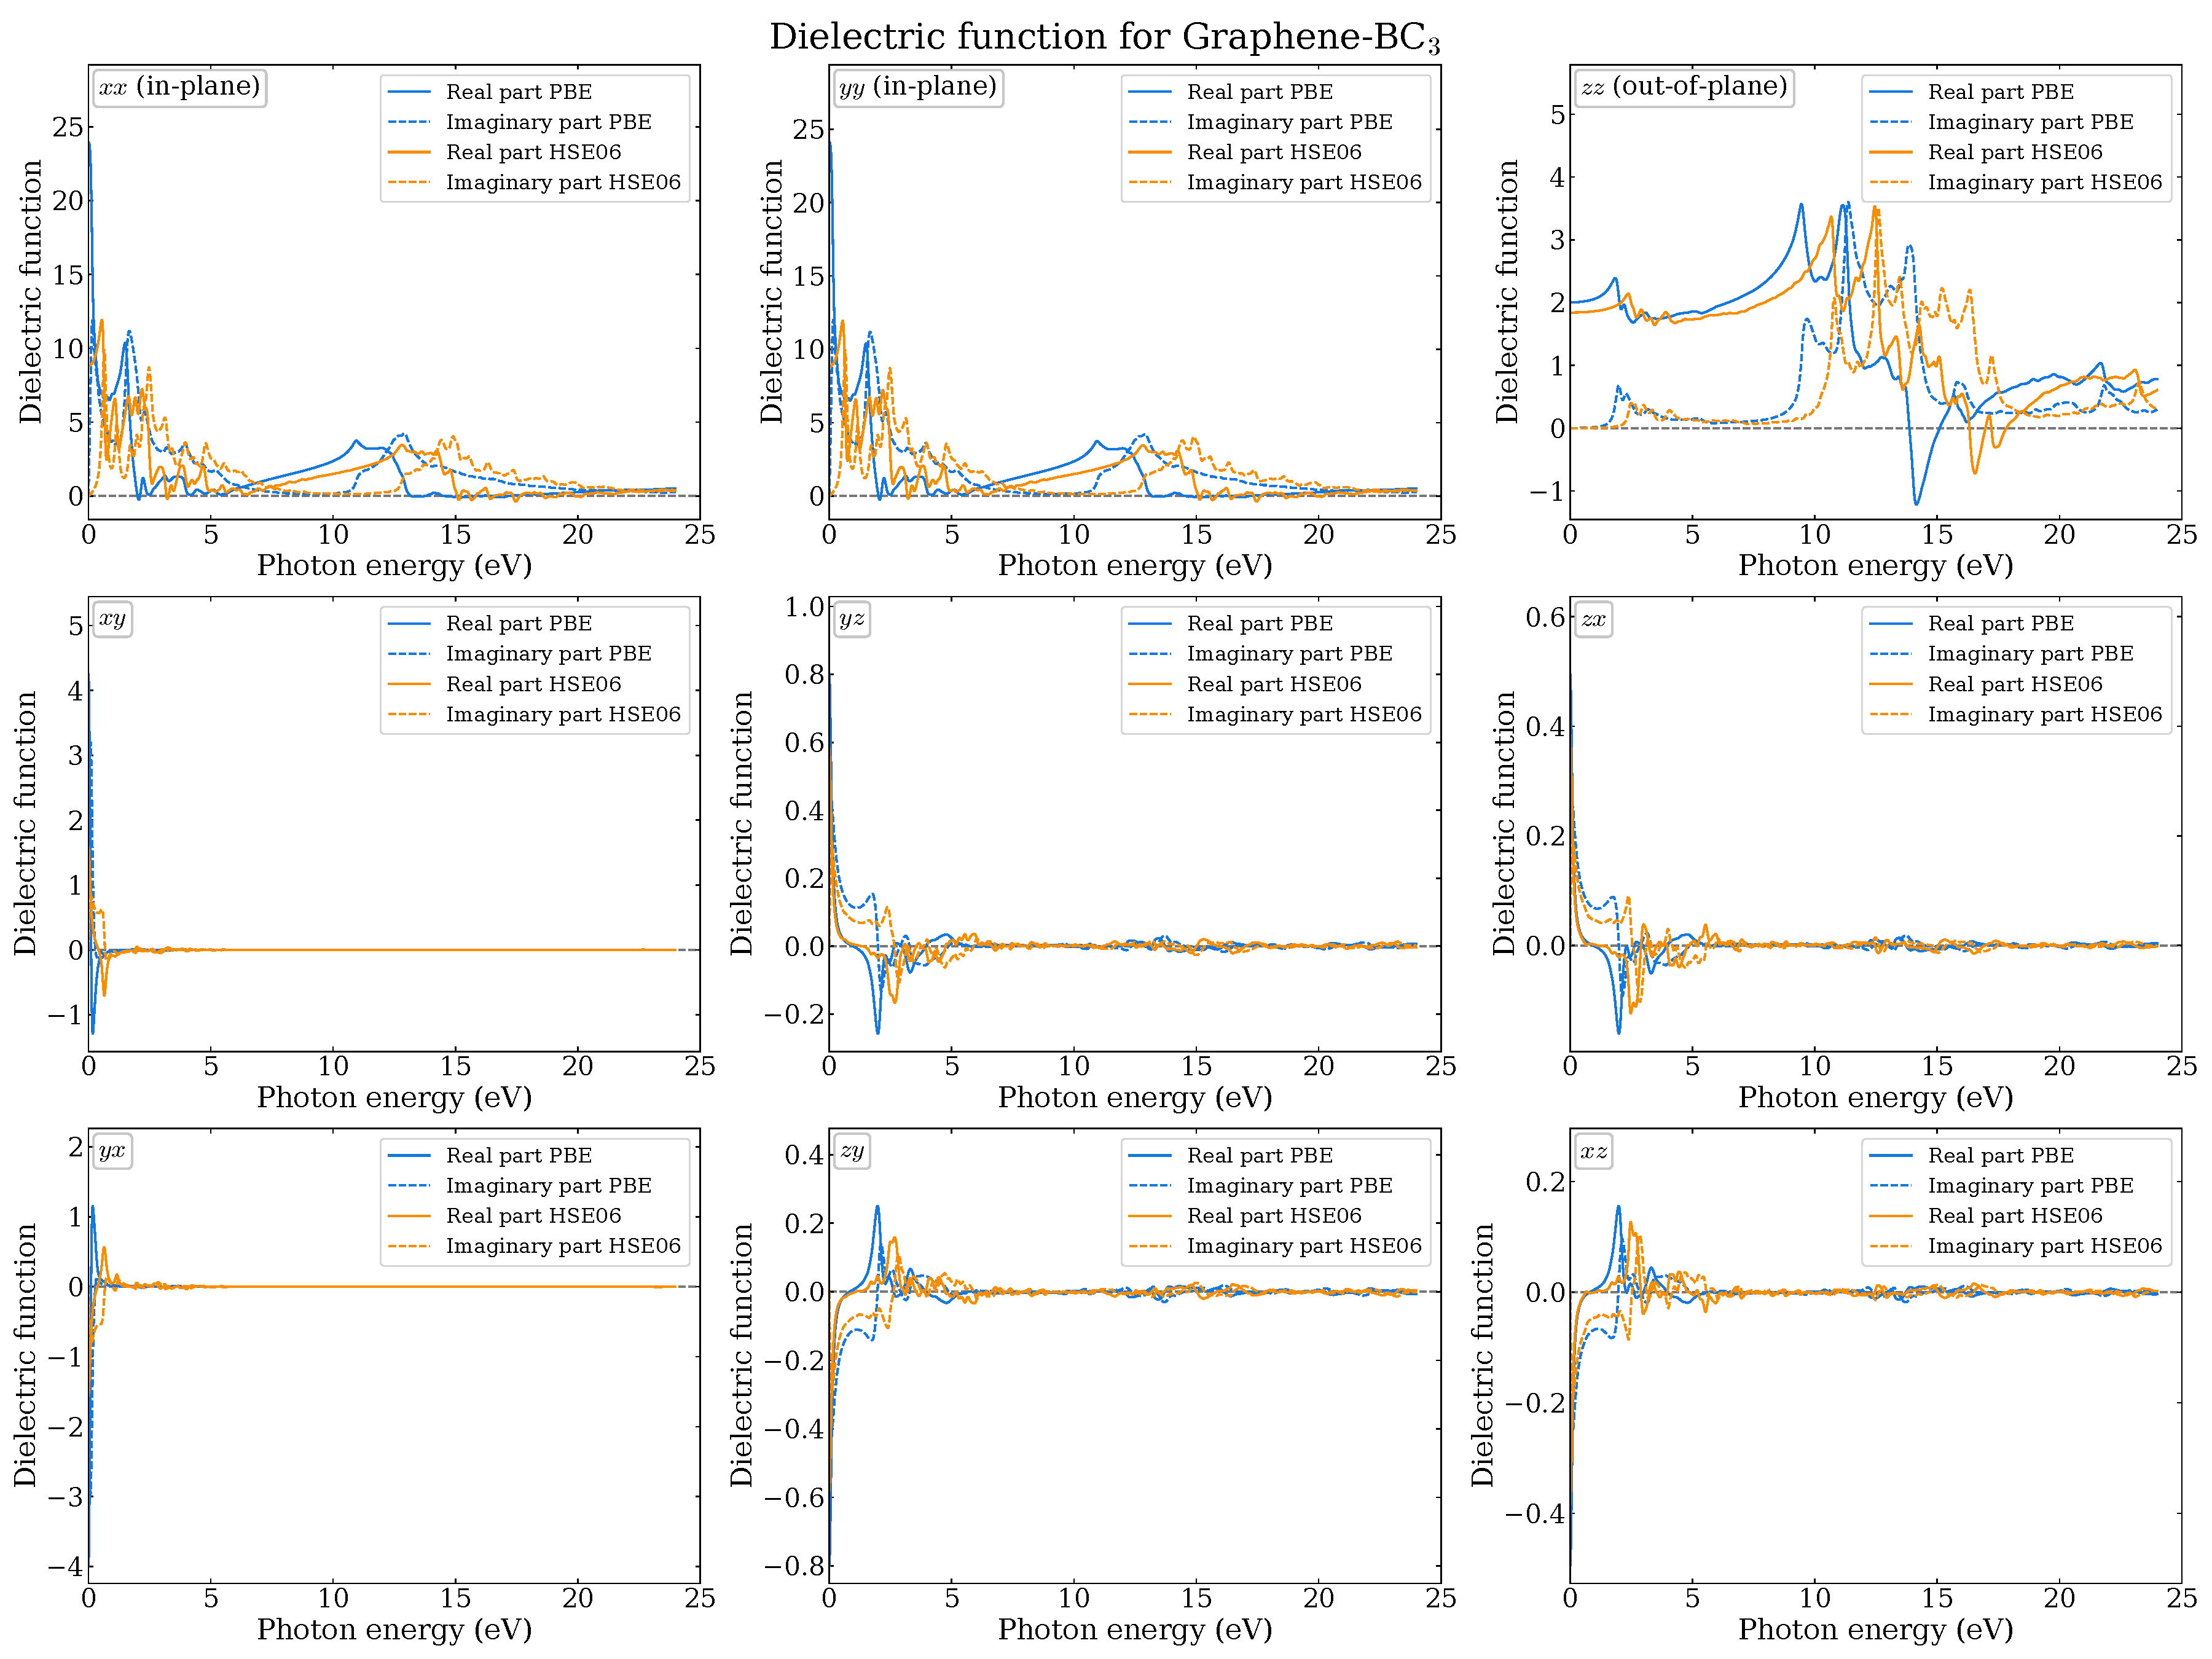
\includegraphics[width=1.00\textwidth]{figures_proj1/S1.18.pdf}
\caption[Dielectric tensor of Graphene-\ce{BC3} calculated using PBE and HSE06.]{Dimensionless dielectric tensor components of Graphene-\ce{BC3} versus photon energy $\hbar\omega$ in \unit{\electronvolt}.
From left to right, the rows show $xx,yy,zz$; $xy,yz,zx$; and $yx,zy,xz$.
The $xx$ and $yy$ directions lie within the layers, while $zz$ is perpendicular to them.
Blue and orange curves denote PBE and HSE06, respectively; solid and dashed lines denote real and imaginary parts.
The HSE06 mesh is $17\times17\times1$.
The displayed off-diagonal response is concentrated at low photon energies.
These entries are shown as exported, and their opposite-sign pairs cancel in the symmetric tensor.}
\label{S1.18}
\end{figure}

\begin{figure}[!htbp]
\centering
    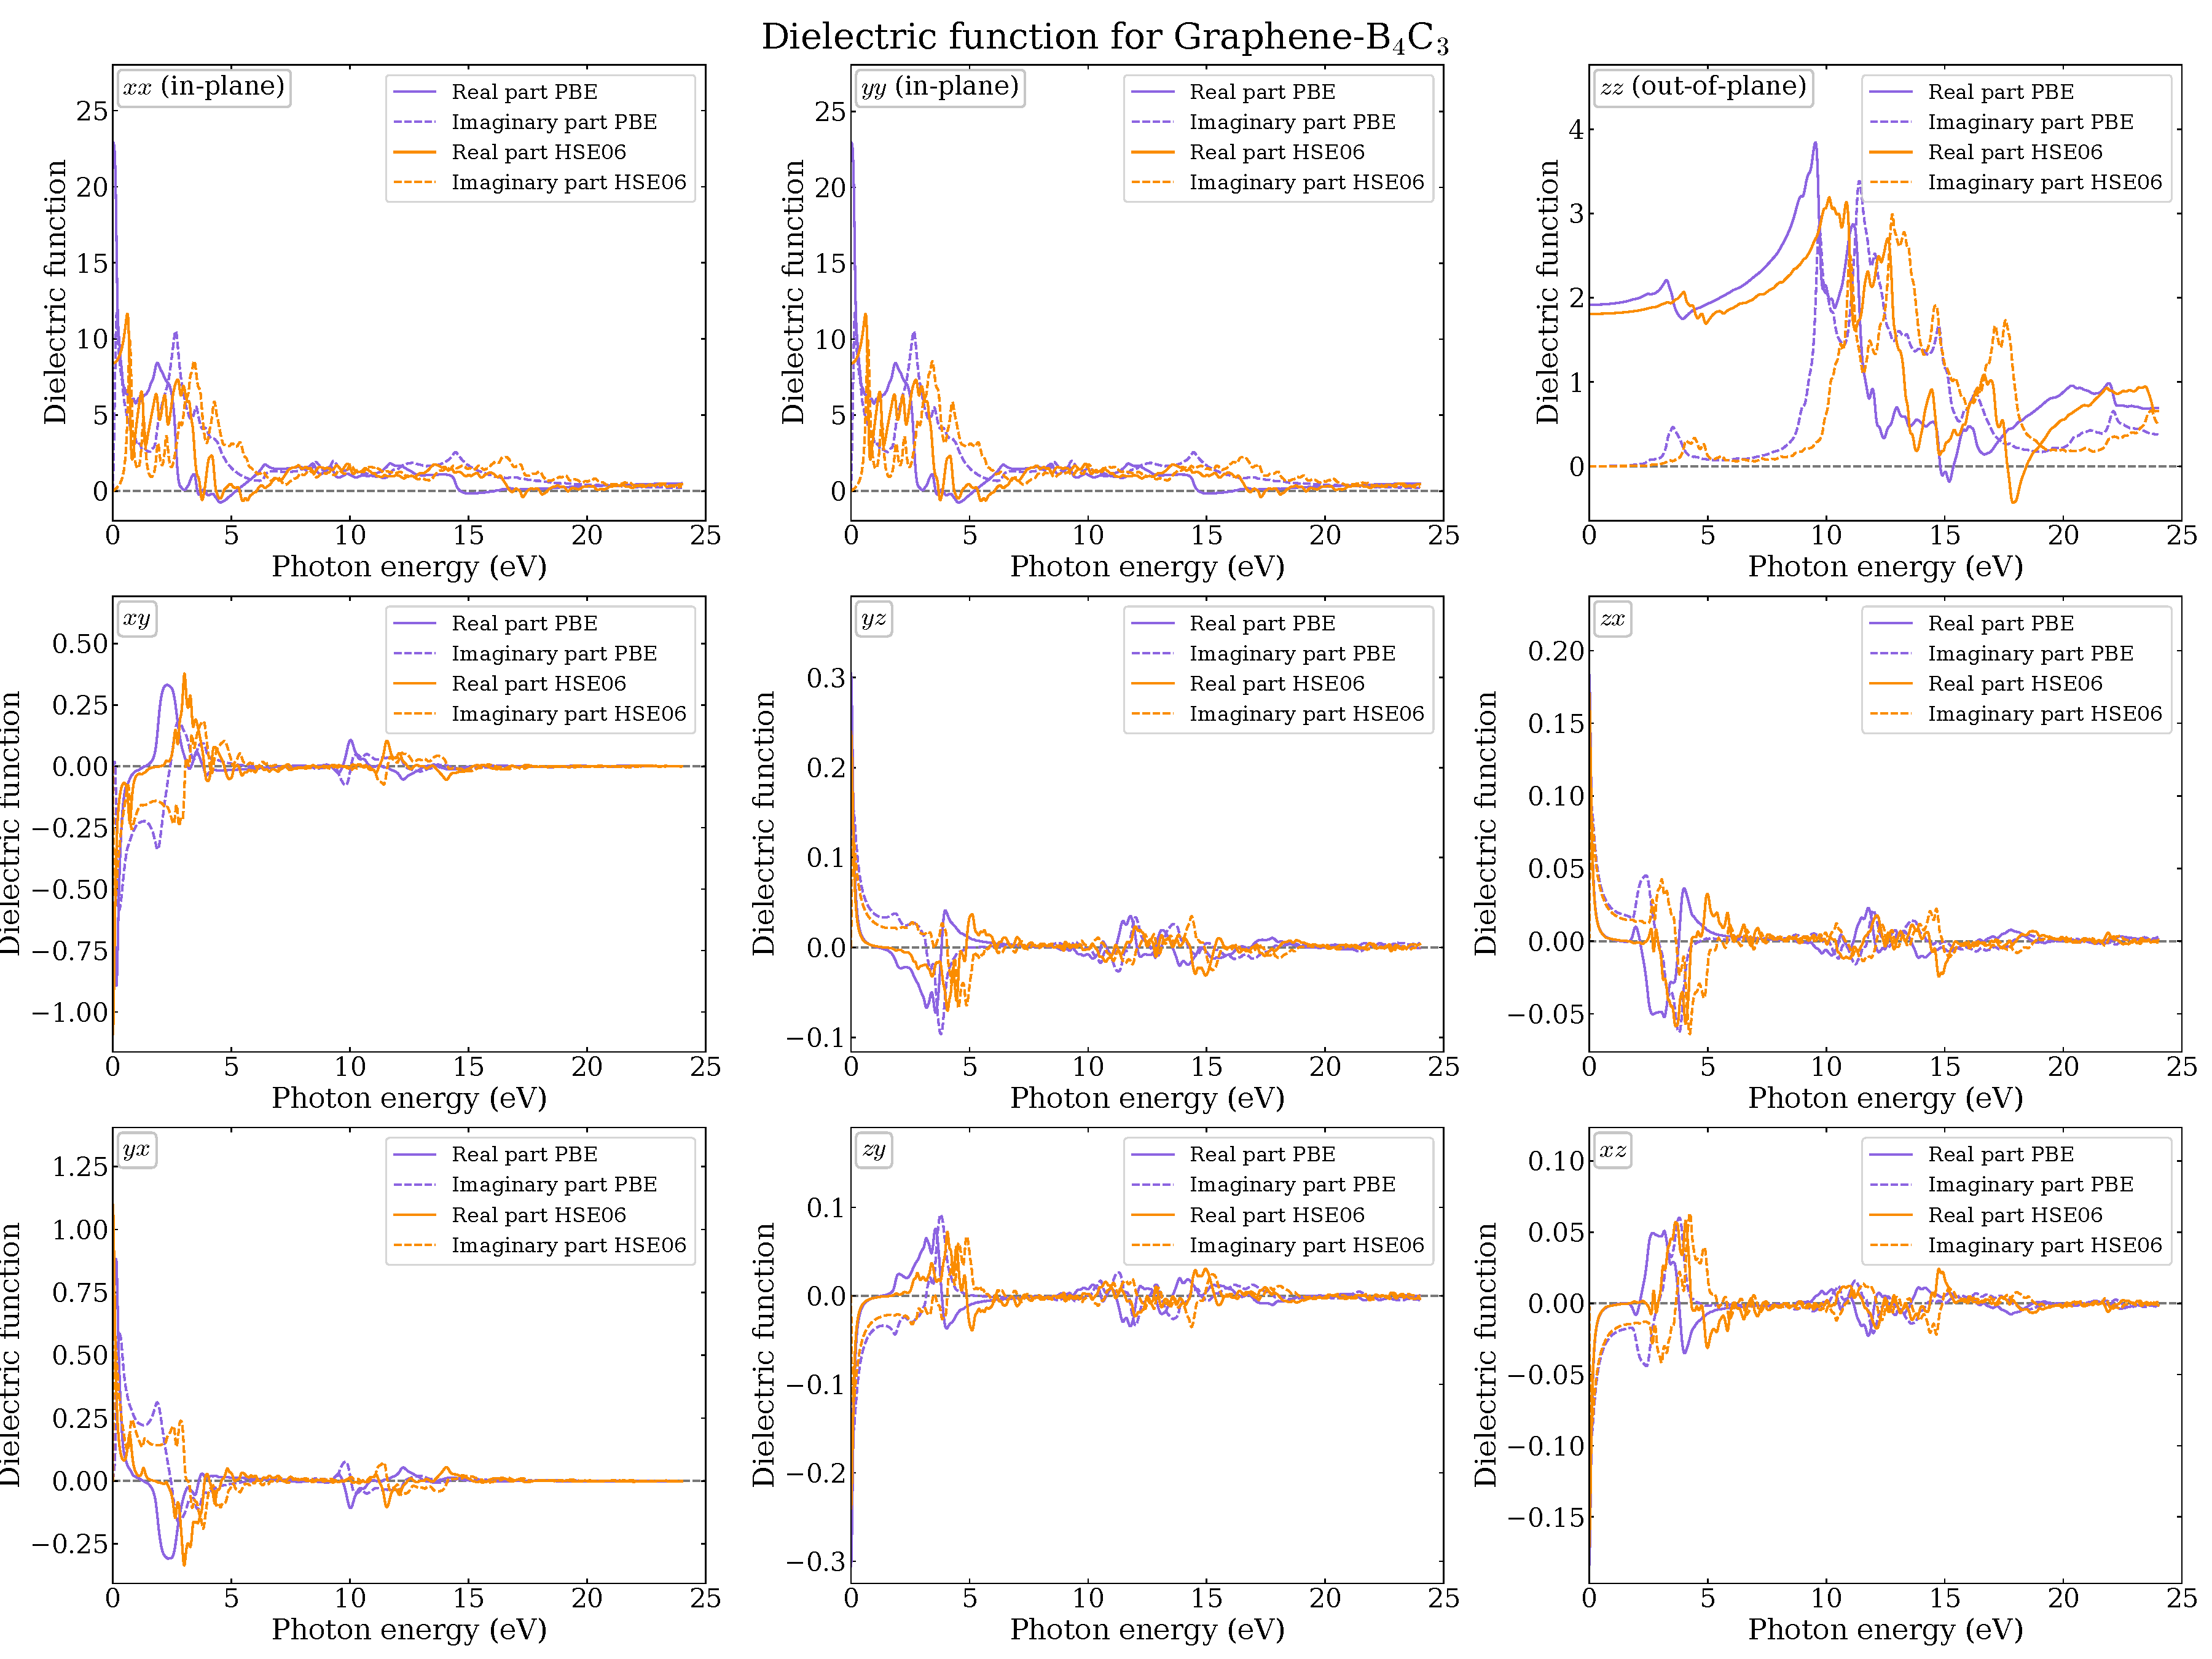
\includegraphics[width=1.00\textwidth]{figures_proj1/S1.19.pdf}
\caption[Dielectric tensor of Graphene-\ce{B4C3} calculated using PBE and HSE06.]{Dimensionless dielectric tensor components of Graphene-\ce{B4C3} versus photon energy $\hbar\omega$ in \unit{\electronvolt}.
From left to right, the rows show $xx,yy,zz$; $xy,yz,zx$; and $yx,zy,xz$.
The $xx$ and $yy$ directions lie within the layers, while $zz$ is perpendicular to them.
Purple and orange curves denote PBE and HSE06, respectively; solid and dashed lines denote real and imaginary parts.
The HSE06 mesh is $17\times17\times1$.
The displayed off-diagonal response extends beyond the low-energy region.
These entries are shown as exported, and their opposite-sign pairs cancel in the symmetric tensor.}
\label{S1.19}
\end{figure}

\begin{figure}[!htbp]
\centering
    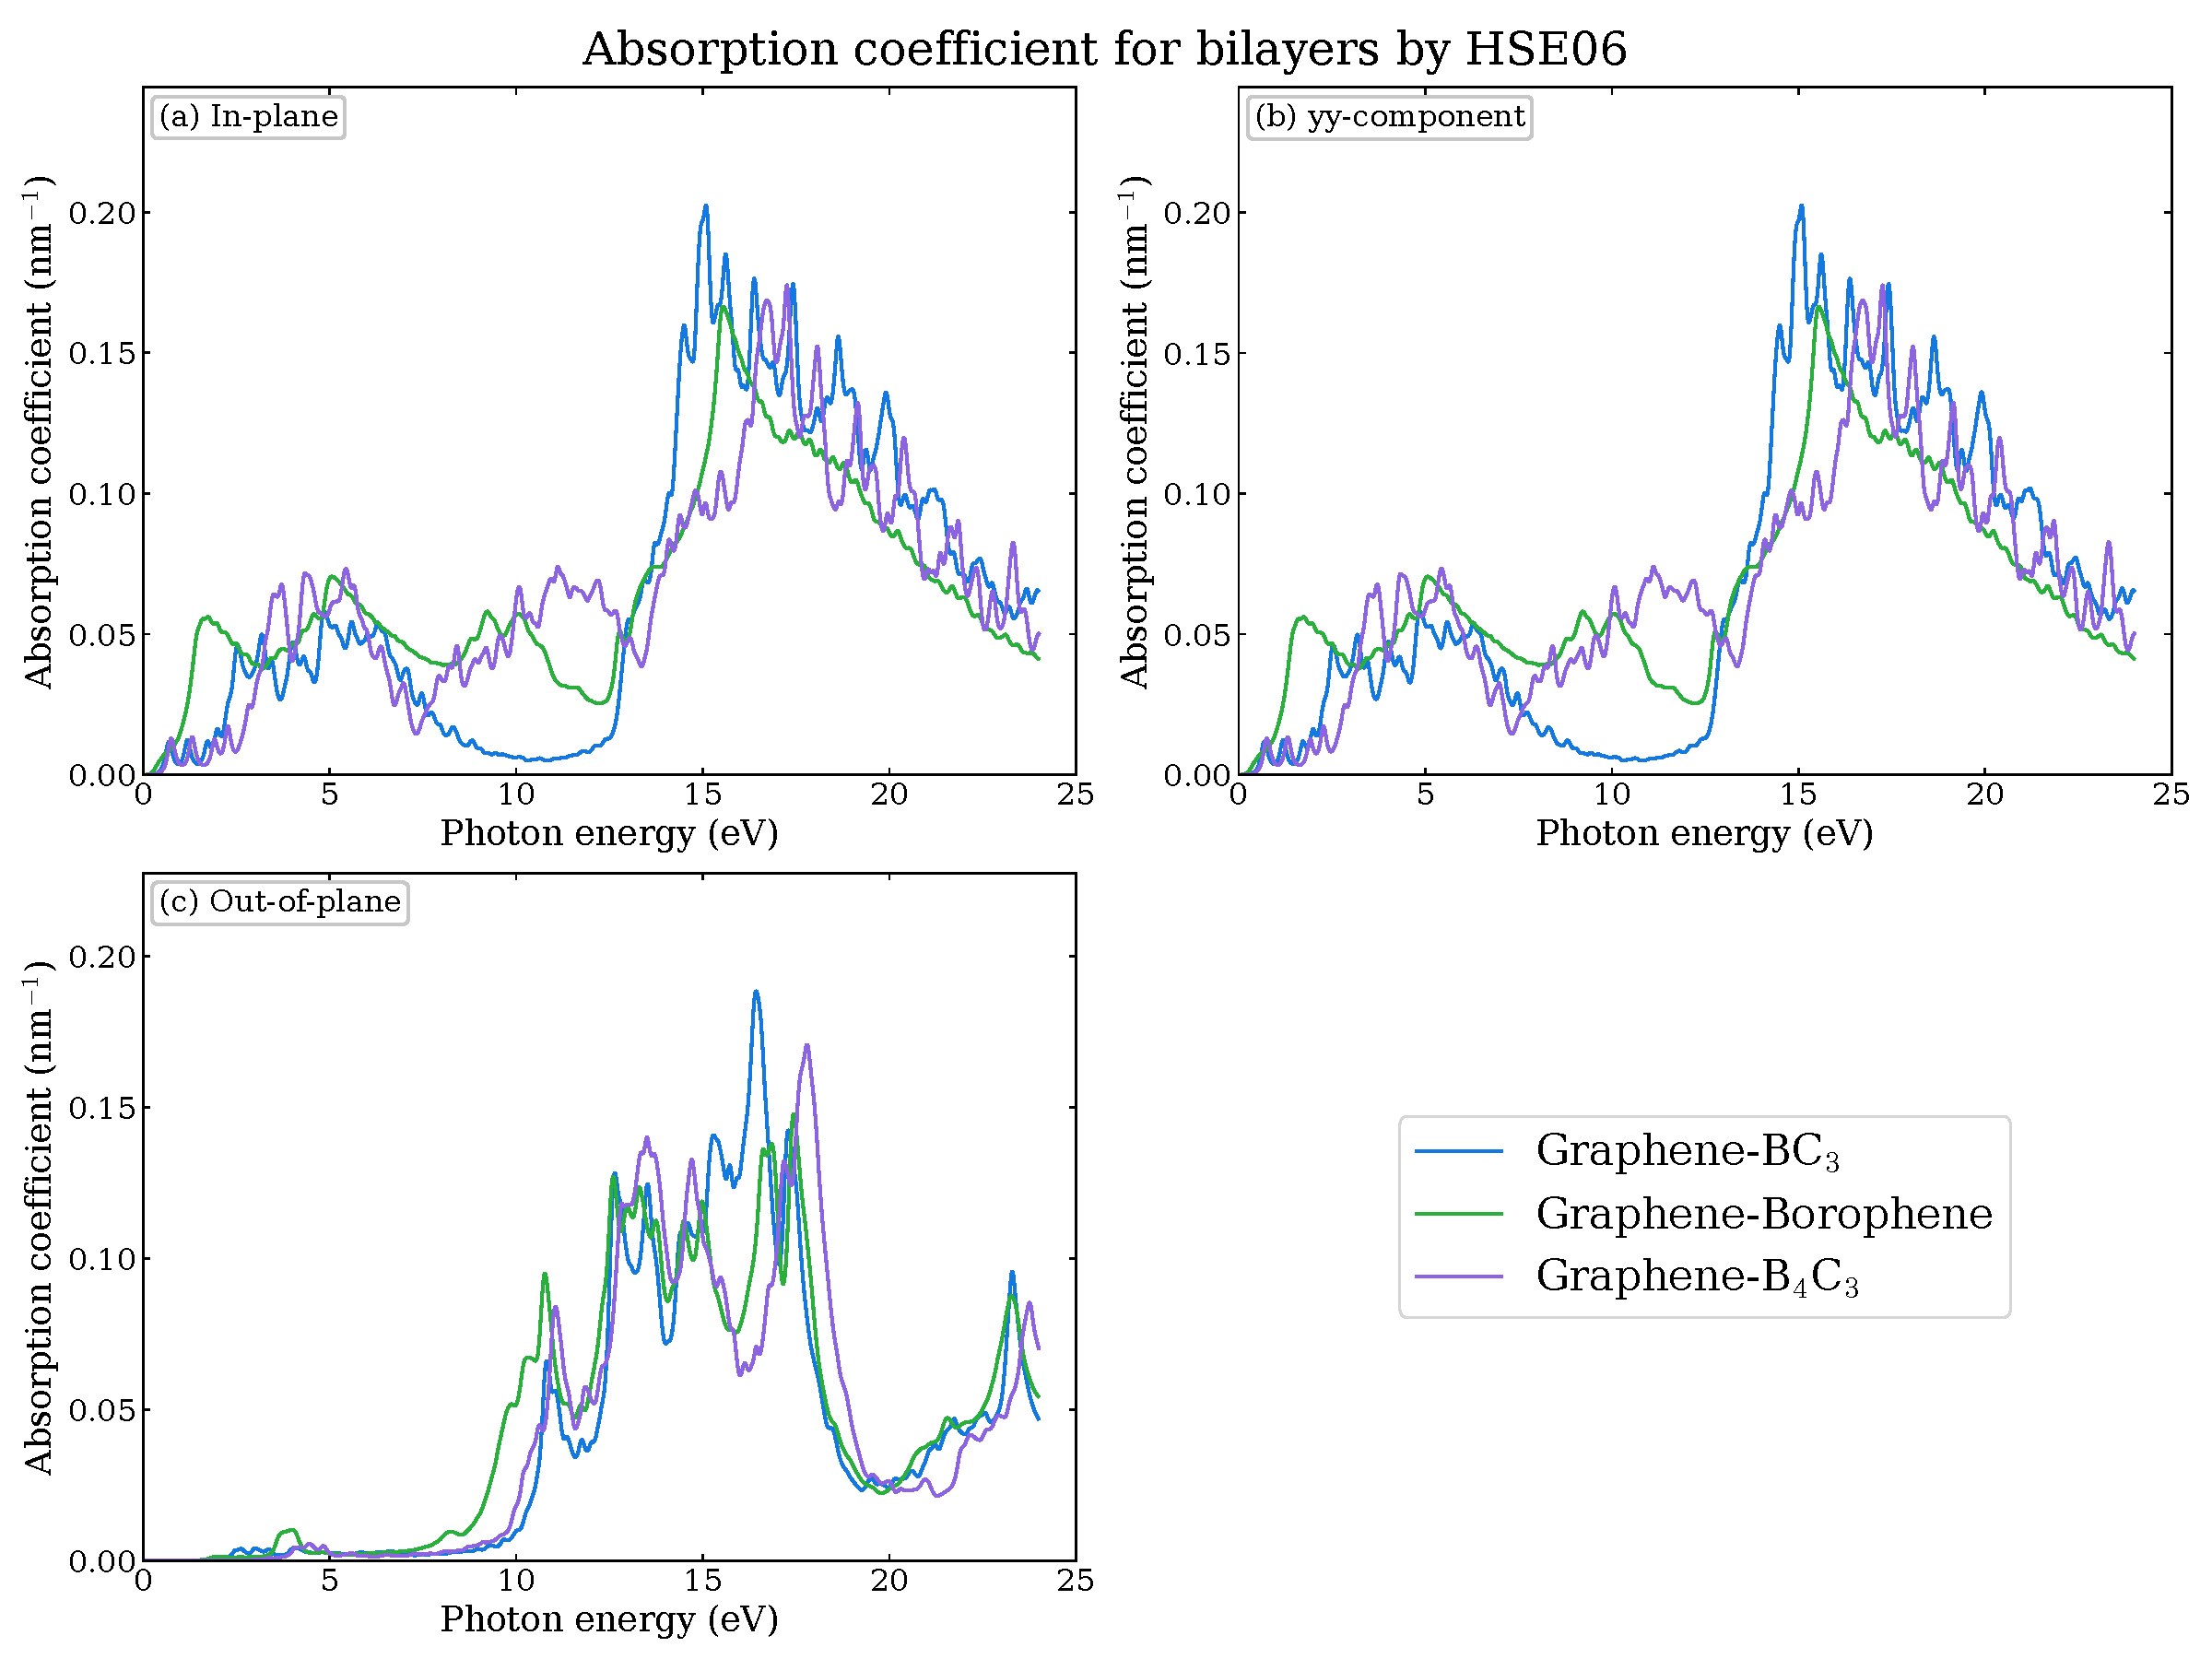
\includegraphics[width=0.80\textwidth]{figures_proj1/S1.20.pdf}
\caption[HSE06 diagonal absorption spectra of the three heterostructure bilayers.]{HSE06 absorption coefficients in \si{\per\nano\metre} for Graphene-\ce{BC3} (blue), Graphene-Borophene (green), and Graphene-\ce{B4C3} (purple).
Panels~(a), (b), and (c) show the diagonal $xx$, $yy$, and $zz$ responses, corresponding to two in-plane polarizations and the out-of-plane polarization, respectively.
All curves are solid and are plotted against photon energy $\hbar\omega$ in \unit{\electronvolt}.
The in-plane response extends into the visible region, while the strongest out-of-plane features occur in the ultraviolet region.}
\label{S1.20}
\end{figure}

\begin{figure}[!htbp]
\centering
    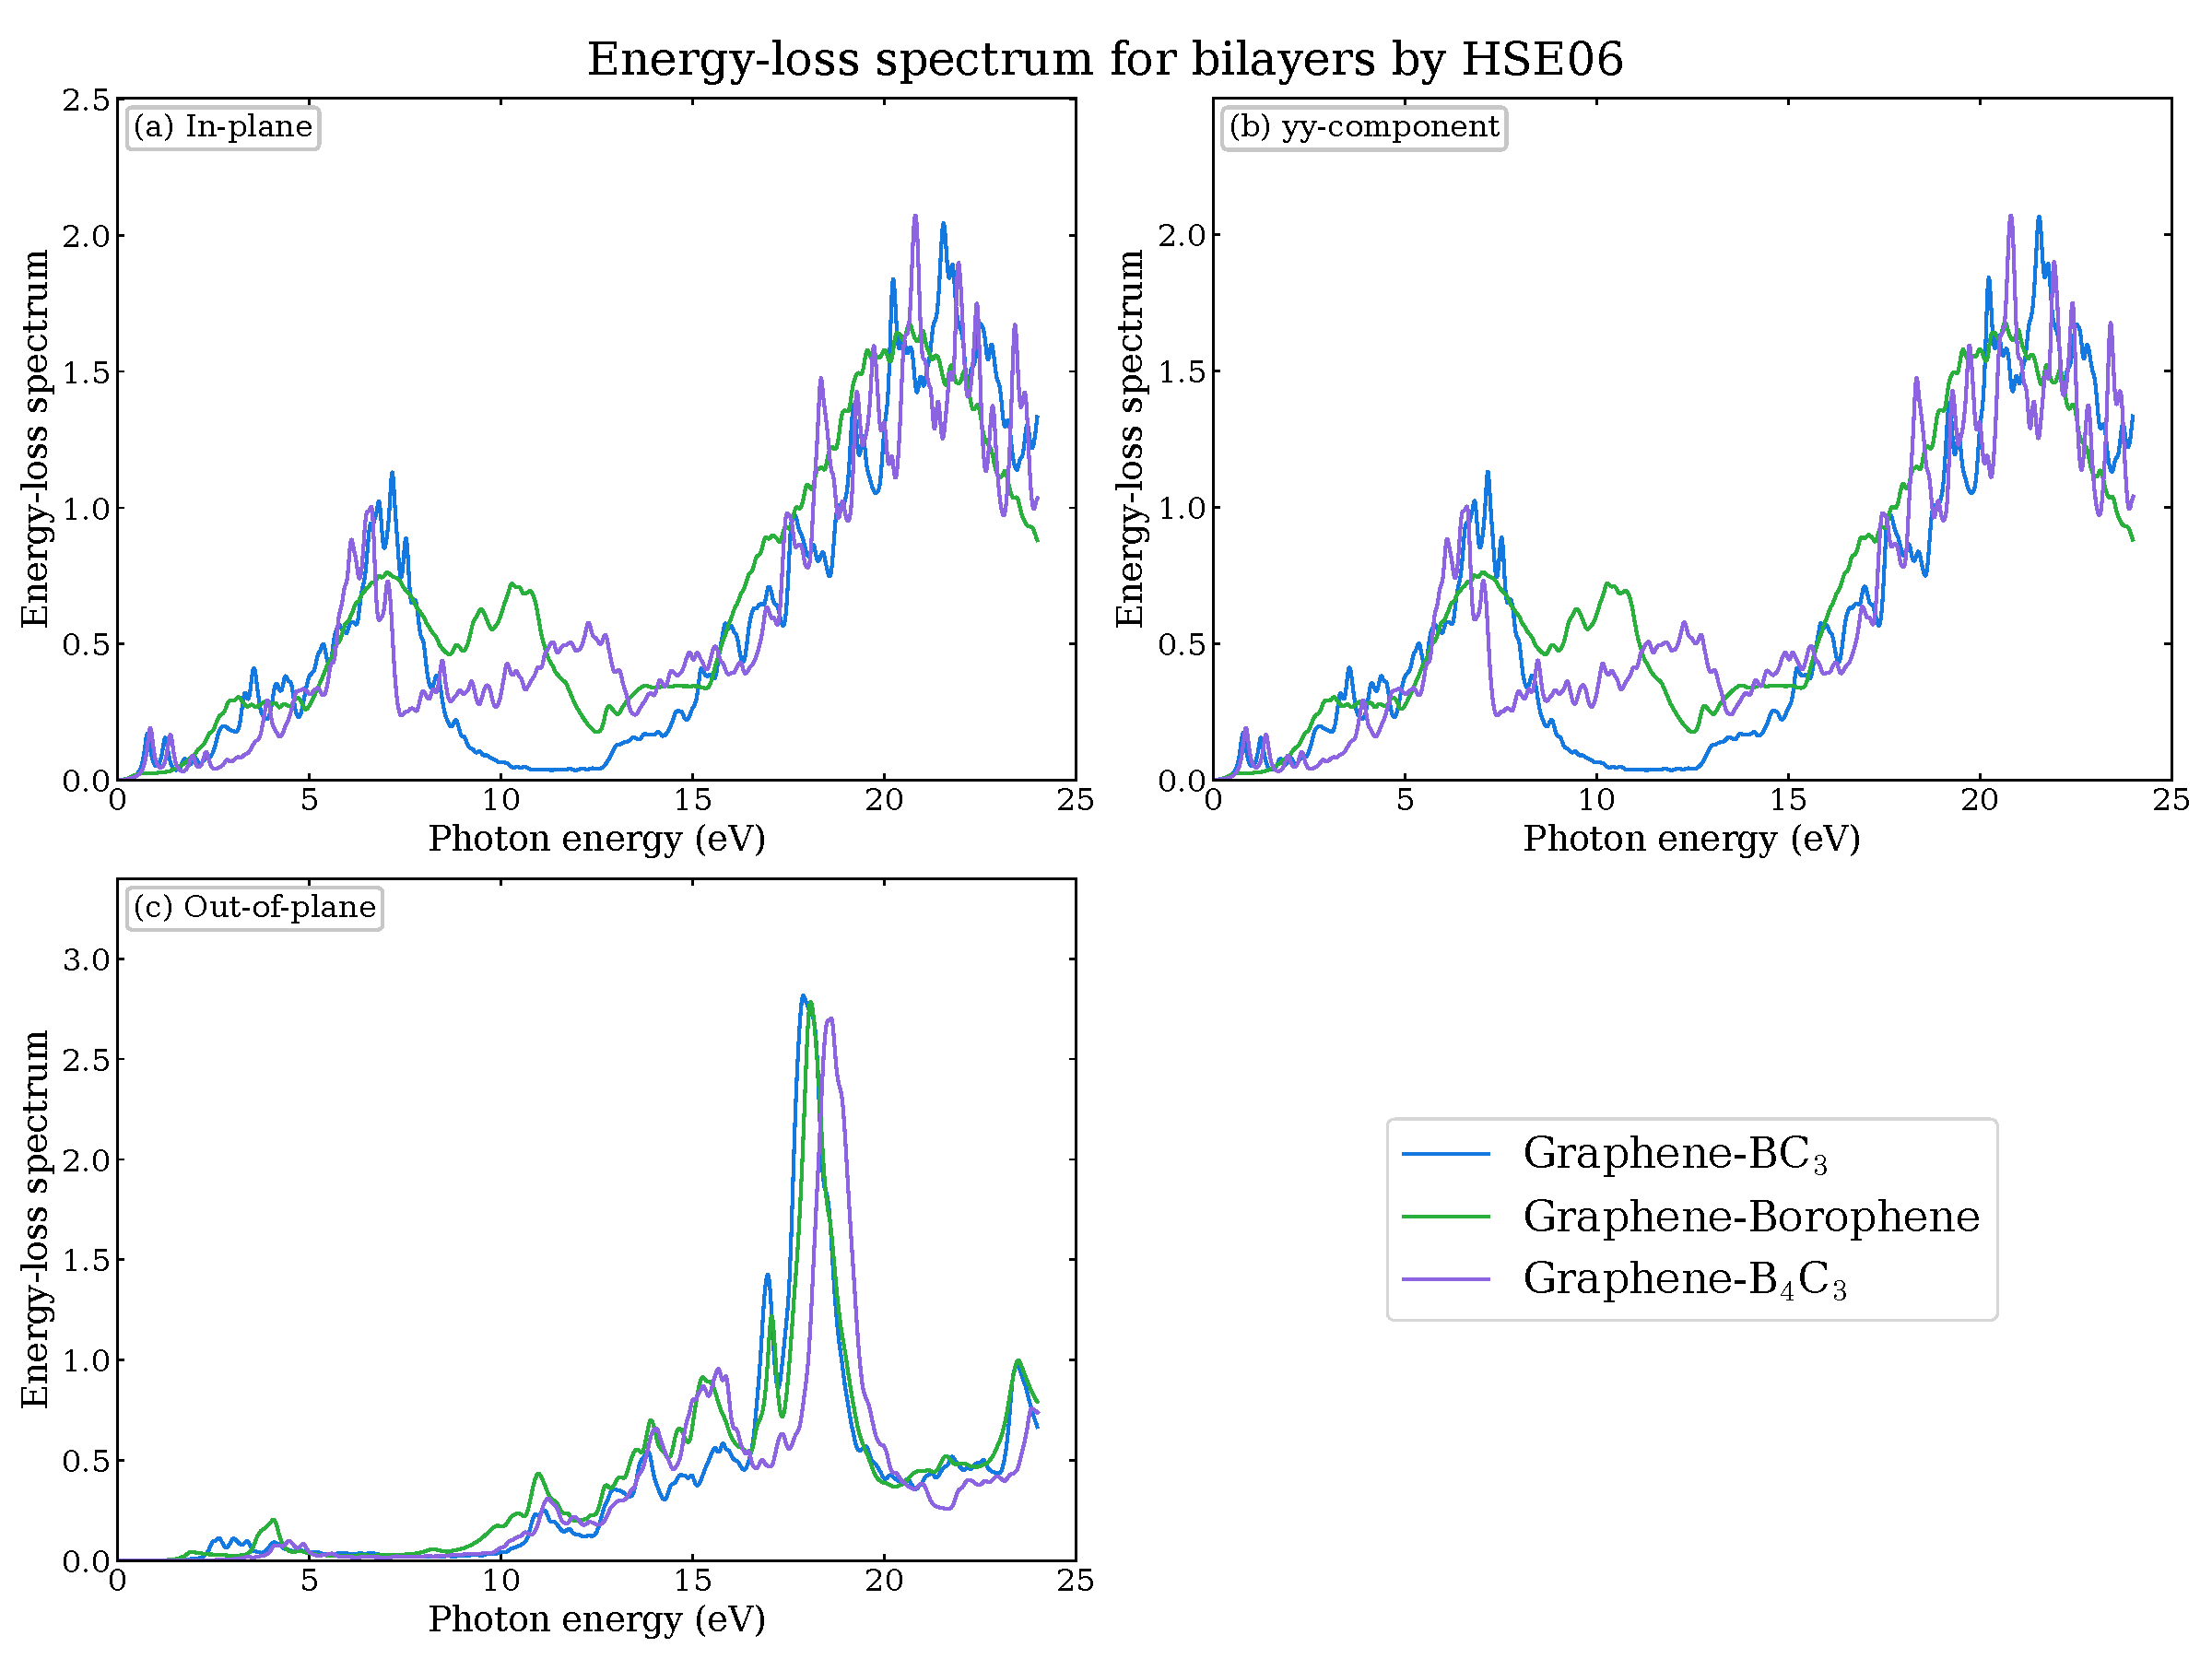
\includegraphics[width=0.80\textwidth]{figures_proj1/S1.21.pdf}
\caption[HSE06 diagonal energy-loss spectra of the three heterostructure bilayers.]{Dimensionless HSE06 energy-loss spectra of Graphene-\ce{BC3} (blue), Graphene-Borophene (green), and Graphene-\ce{B4C3} (purple).
Panels~(a), (b), and (c) show the diagonal $xx$, $yy$, and $zz$ responses, corresponding to two in-plane directions and the out-of-plane direction.
All curves are solid and are plotted against photon energy $\hbar\omega$ in \unit{\electronvolt}.
The strongest out-of-plane loss features occur around \qtyrange{17}{19}{\electronvolt}.}
\label{S1.21}
\end{figure}

\begin{figure}[!htbp]
\centering
    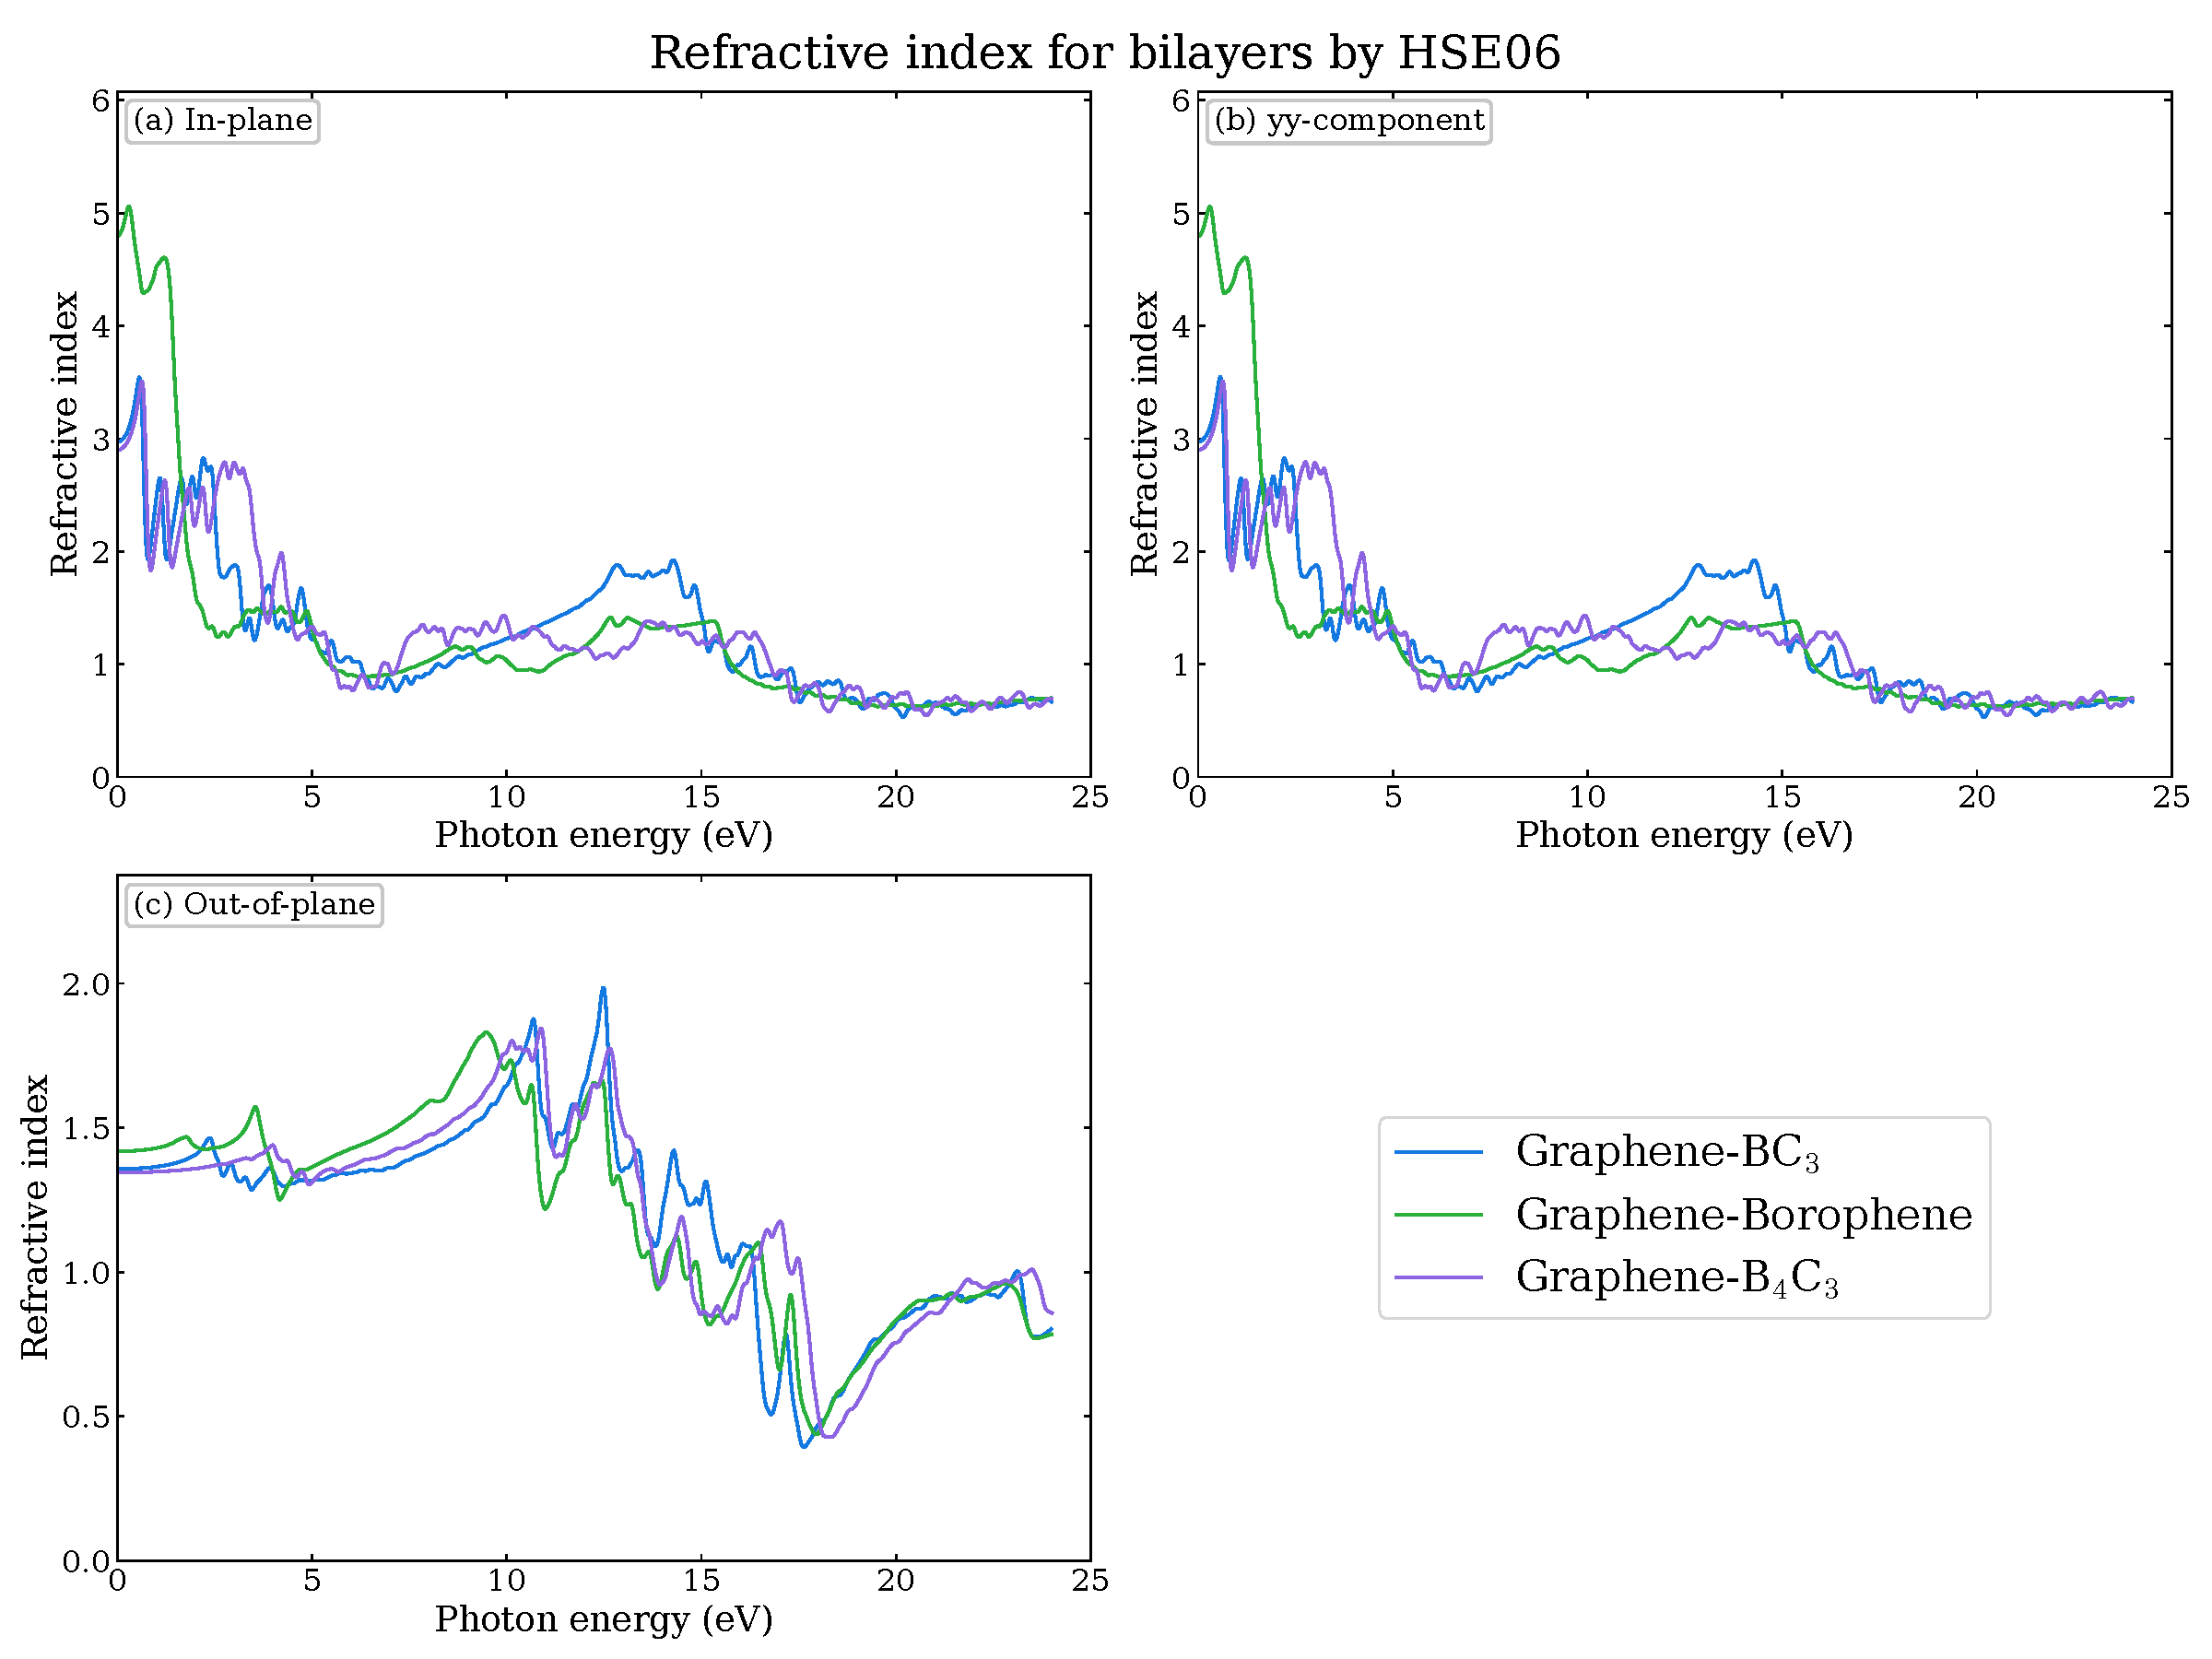
\includegraphics[width=0.80\textwidth]{figures_proj1/S1.22.pdf}
\caption[HSE06 diagonal refractive indices of the three heterostructure bilayers.]{Dimensionless HSE06 refractive indices of Graphene-\ce{BC3} (blue), Graphene-Borophene (green), and Graphene-\ce{B4C3} (purple).
Panels~(a), (b), and (c) show the diagonal $xx$, $yy$, and $zz$ responses, corresponding to two in-plane polarizations and the out-of-plane polarization.
All curves are solid and are plotted against photon energy $\hbar\omega$ in \unit{\electronvolt}.
The largest in-plane indices occur at low photon energies; the out-of-plane maxima occur at higher energies.}
\label{S1.22}
\end{figure}

\begin{figure}[!htbp]
\centering
    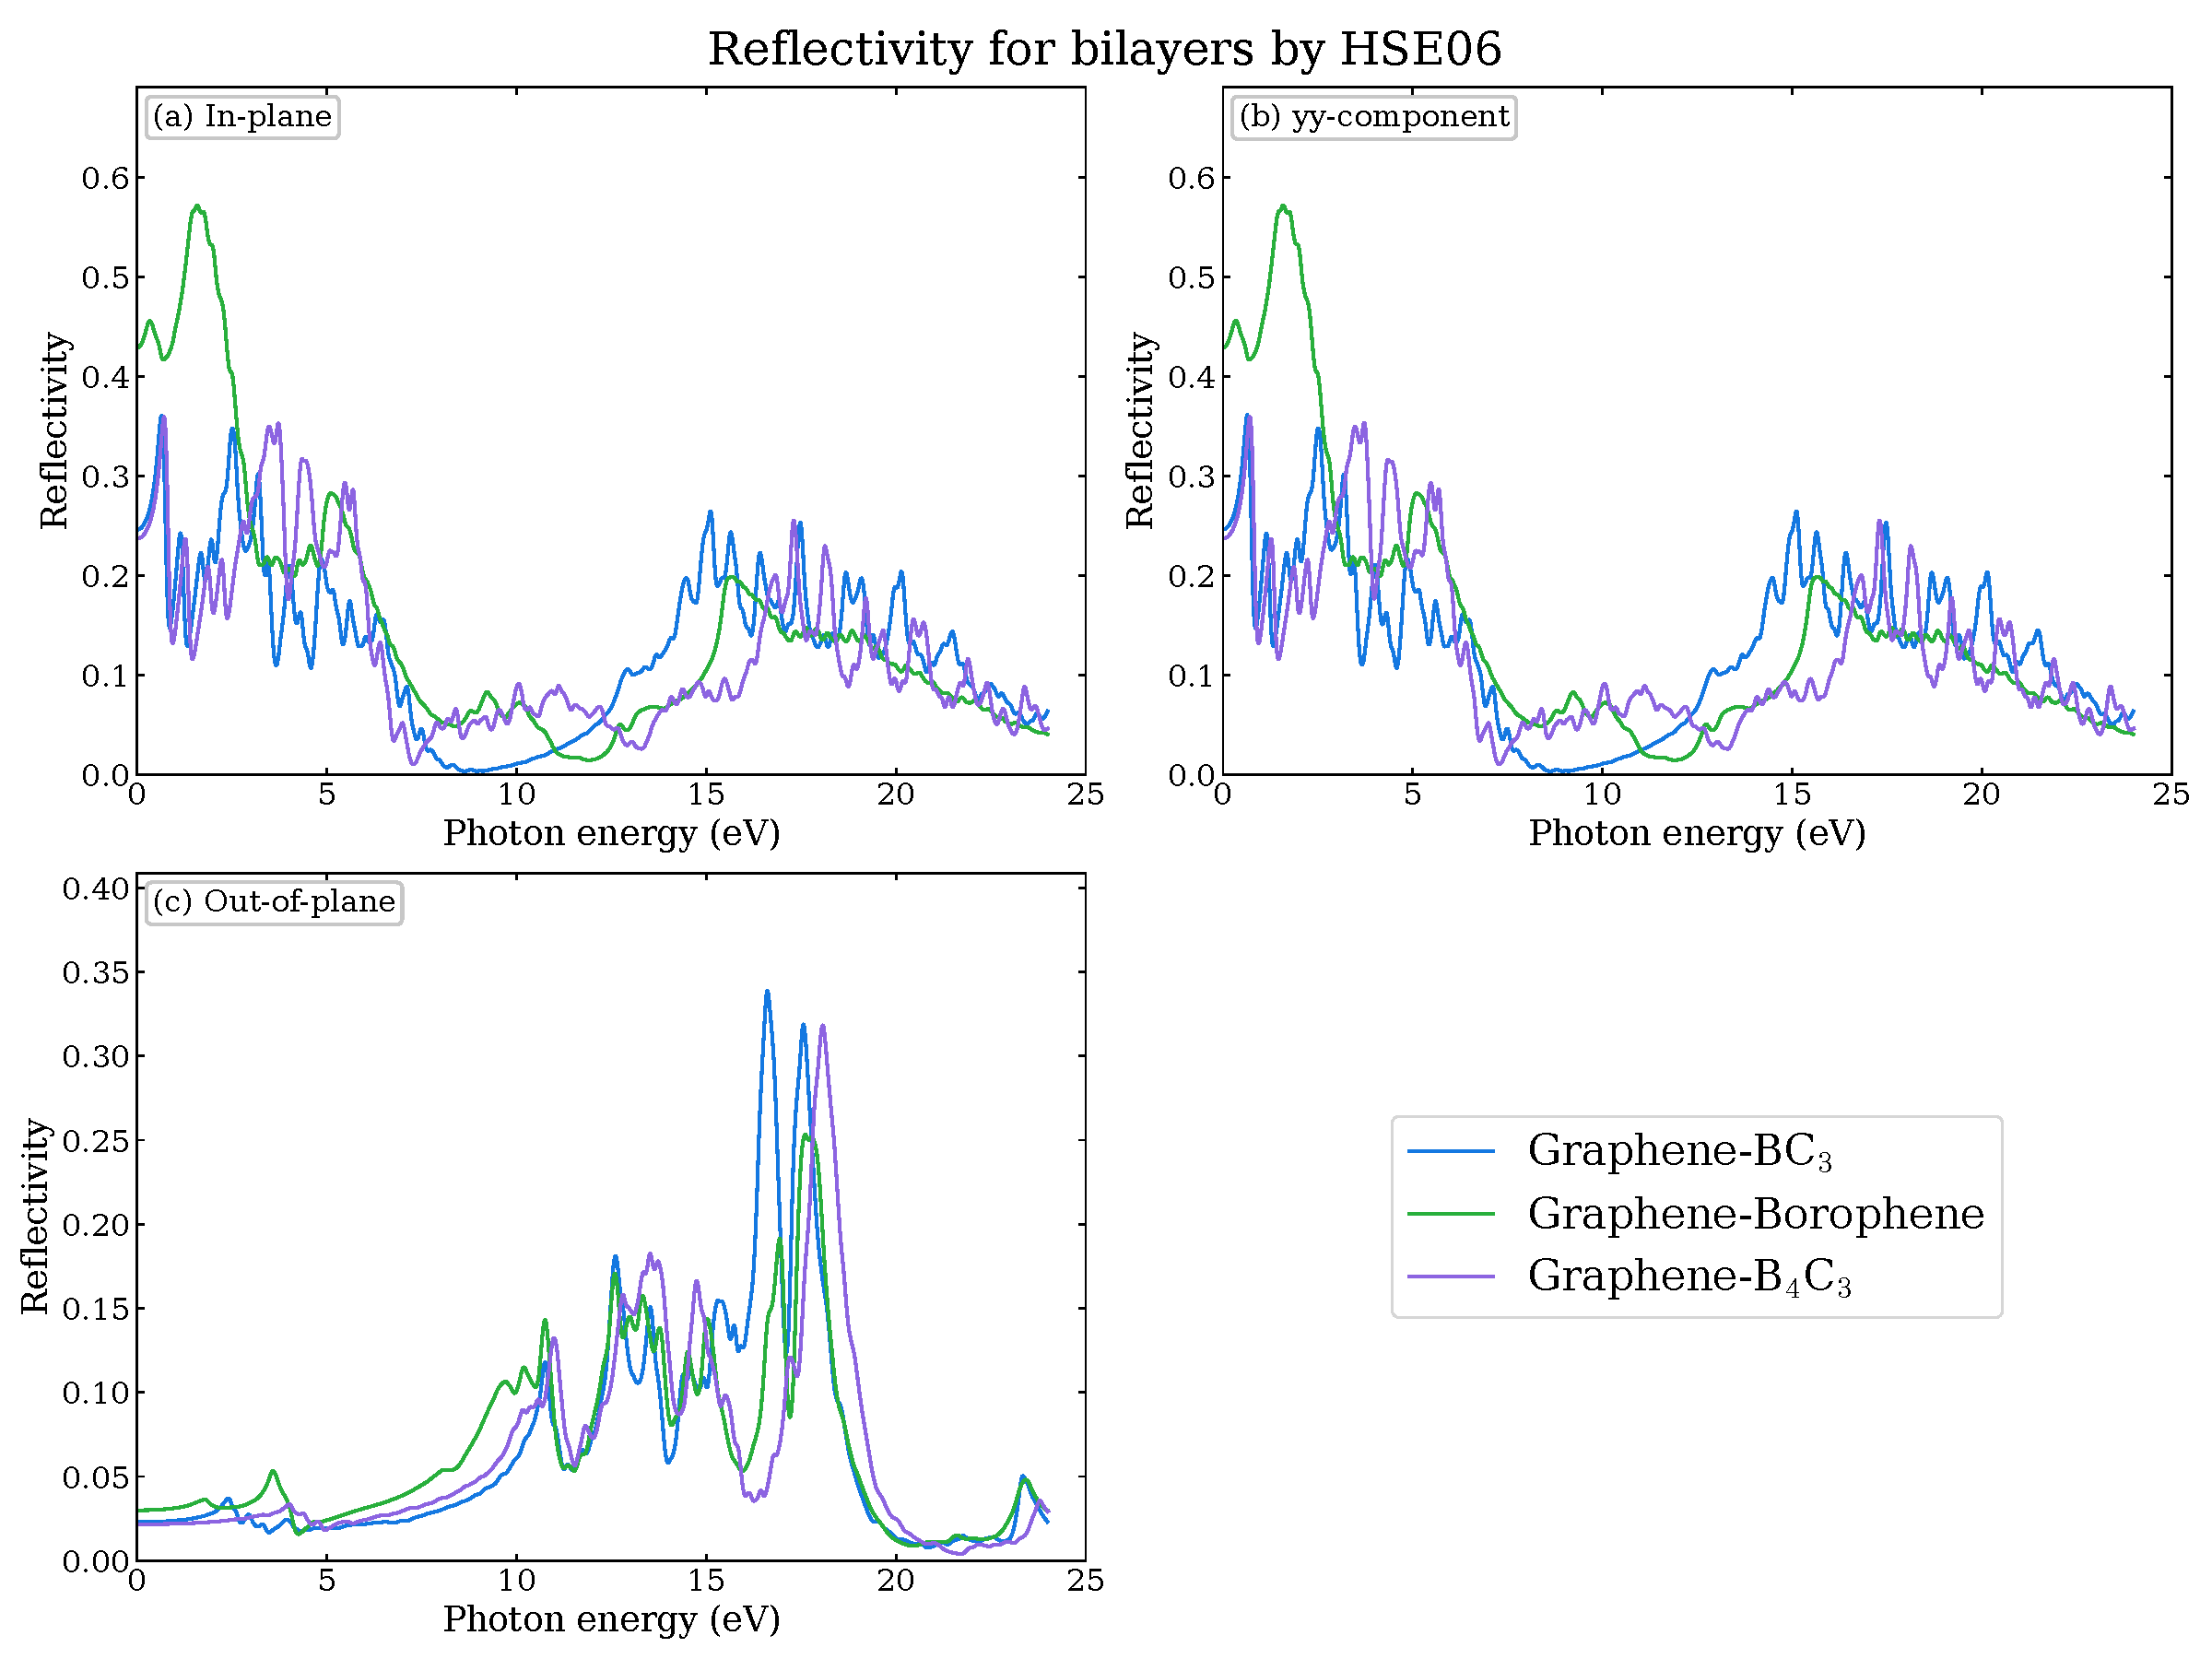
\includegraphics[width=0.80\textwidth]{figures_proj1/S1.23_correct.pdf}
\caption[HSE06 diagonal reflectivities of the three heterostructure bilayers.]{Dimensionless HSE06 reflectivities of Graphene-\ce{BC3} (blue), Graphene-Borophene (green), and Graphene-\ce{B4C3} (purple), evaluated in the principal-axis effective-medium description.
Panels~(a), (b), and (c) show the diagonal $xx$, $yy$, and $zz$ responses, corresponding to two in-plane polarizations and the out-of-plane polarization.
All curves are solid and are plotted against photon energy $\hbar\omega$ in \unit{\electronvolt}.
The out-of-plane peaks occur in the ultraviolet region.}
\label{S1.23}
\end{figure}

\begin{figure}[!htbp]
\centering
    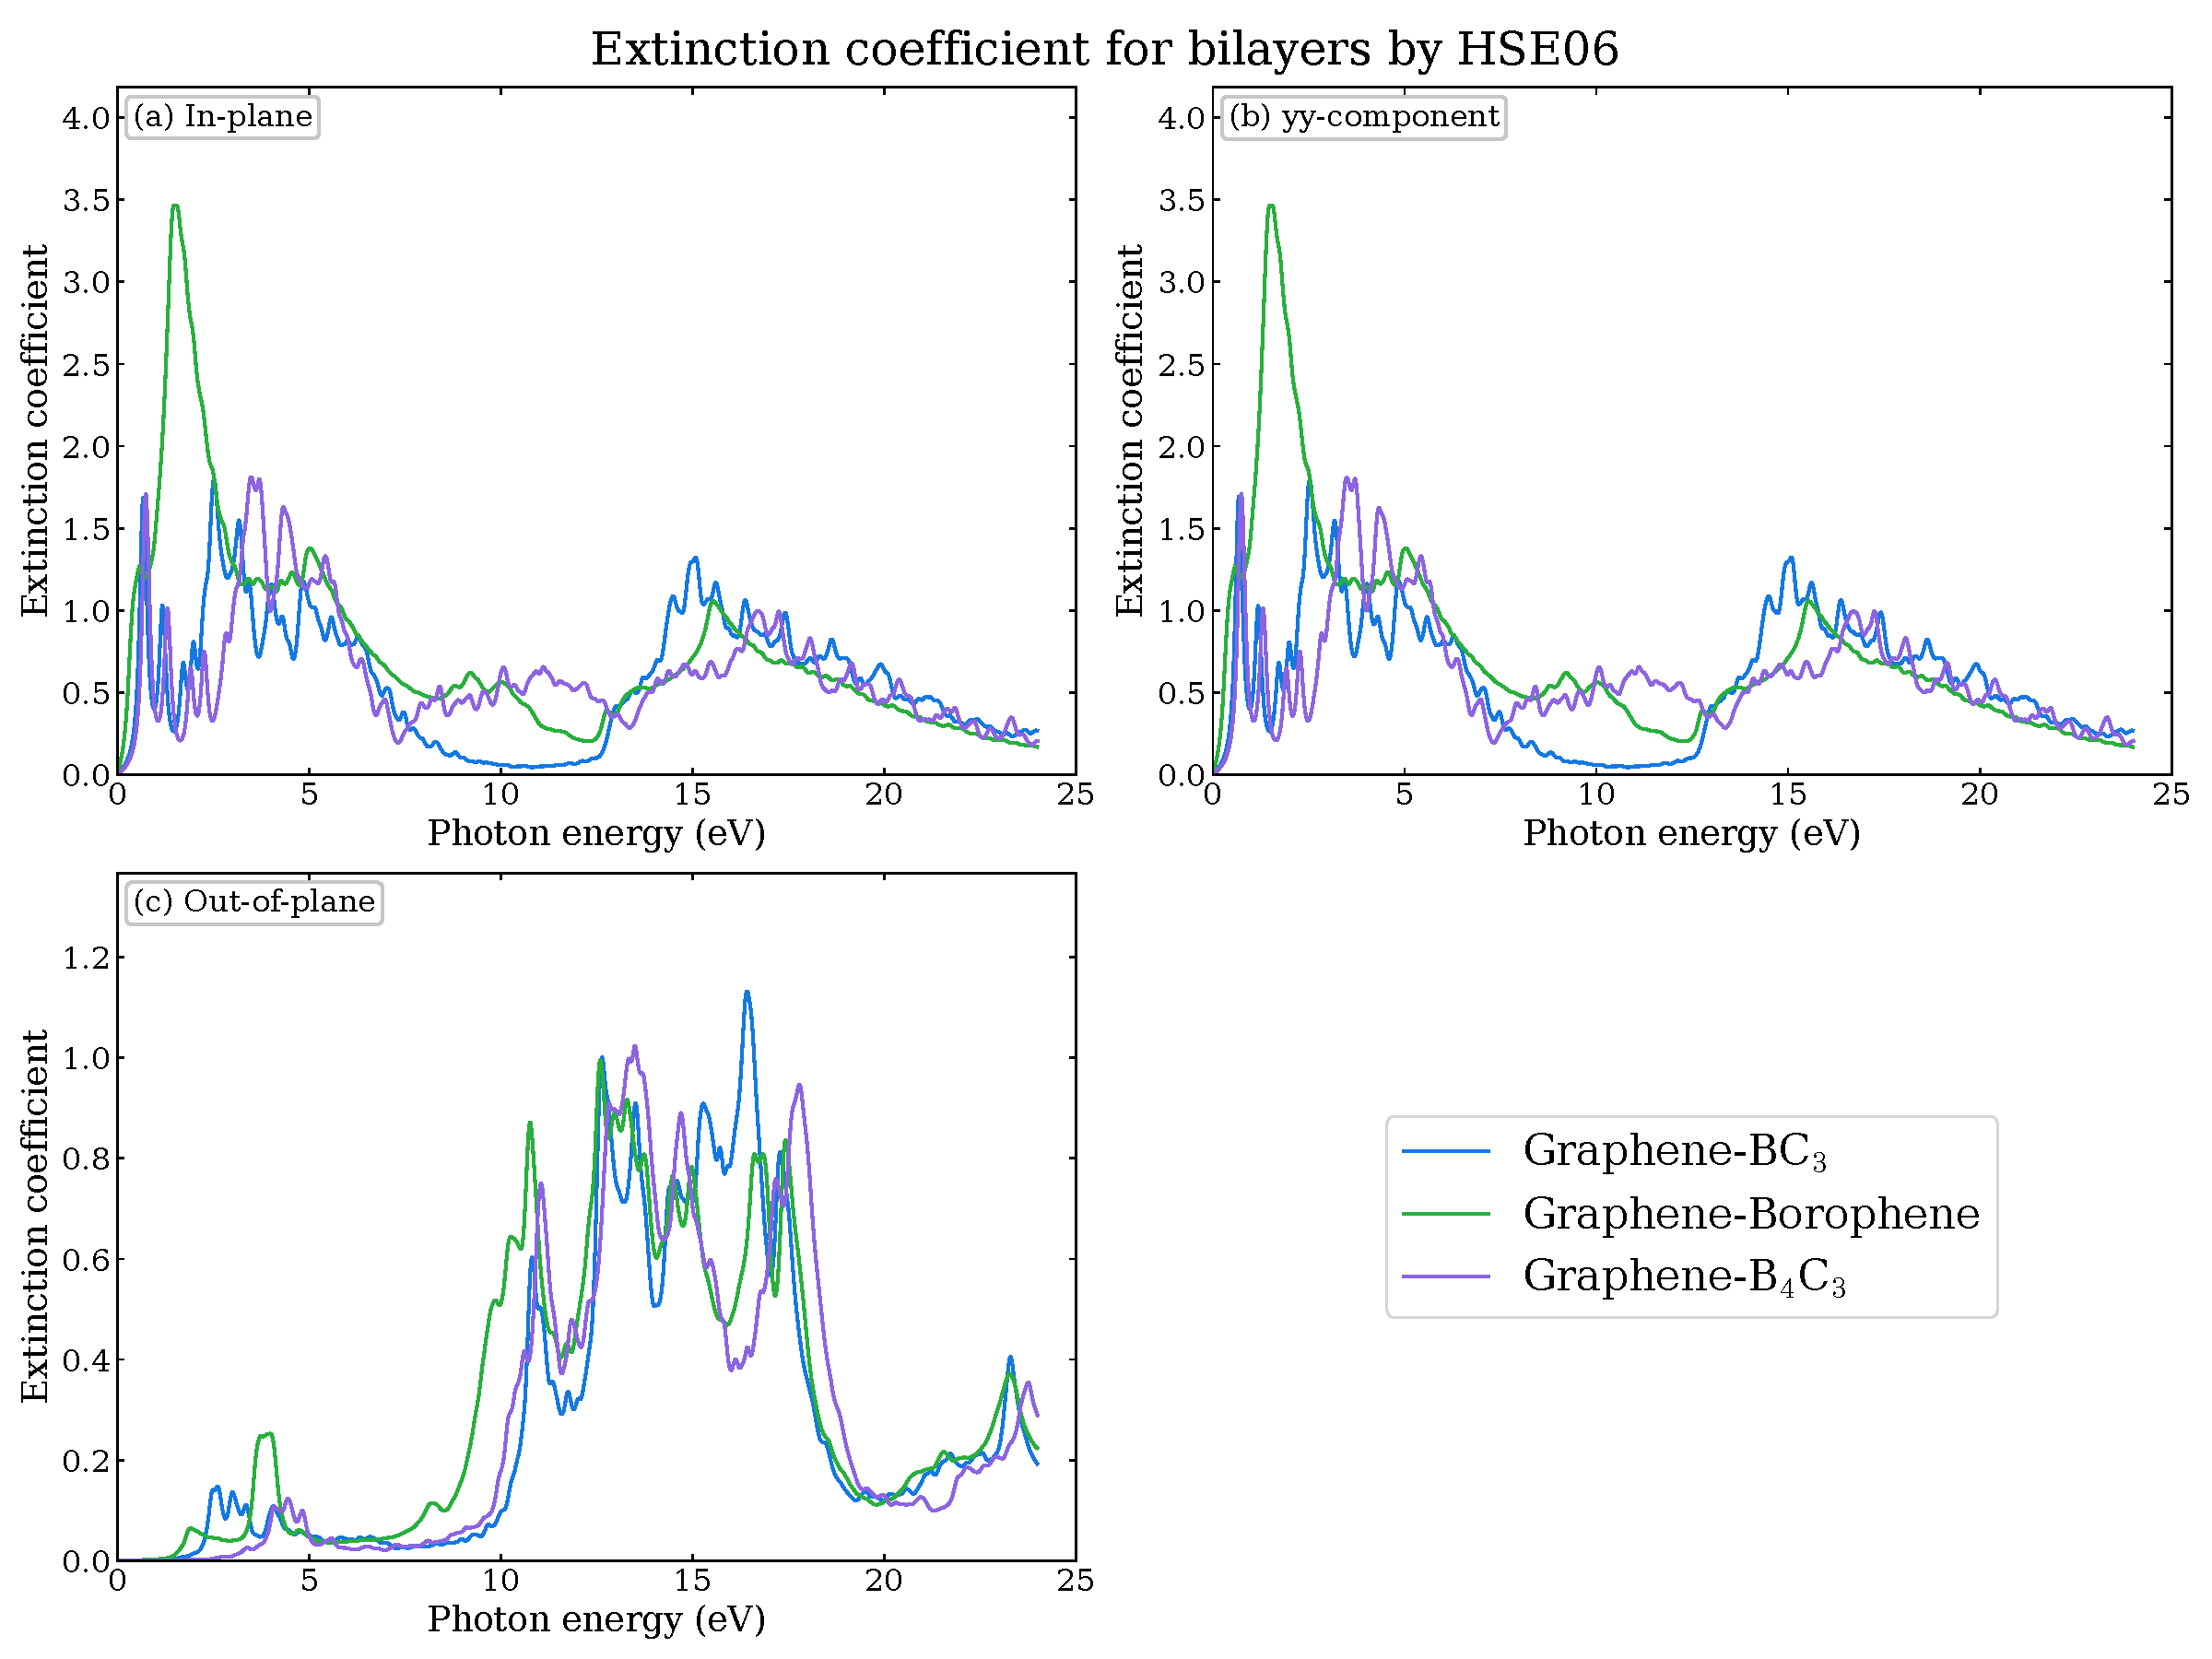
\includegraphics[width=0.80\textwidth]{figures_proj1/S1.24_correct.pdf}
\caption[HSE06 diagonal extinction coefficients of the three heterostructure bilayers.]{Dimensionless HSE06 extinction coefficients of Graphene-\ce{BC3} (blue), Graphene-Borophene (green), and Graphene-\ce{B4C3} (purple).
Panels~(a), (b), and (c) show the diagonal $xx$, $yy$, and $zz$ responses, corresponding to two in-plane polarizations and the out-of-plane polarization.
All curves are solid and are plotted against photon energy $\hbar\omega$ in \unit{\electronvolt}.
The principal in-plane features occur at lower energies than the broad out-of-plane peaks.}
\label{S1.24}
\end{figure}

\cleardoublepage
\chapter[Functional Properties of Penta-Bipyramid Boron Phases]{Superconductivity, Magnetism, and Directional Plasmonic Modes in Two-Dimensional Penta-Bipyramid Boron Allotropes}
\label{cha:project_boron}

This chapter is based on the article by L. Niu, O. J. Conquest, H. Ma, C. Verdi, and C. Stampfl,
published in \textit{Physical Review Materials} \textbf{10}, 074001 (2026)~\cite{niu2026superconductivity}.
The candidate carried out the calculations, data analysis, and visualization.
Oliver James Conquest guided the molecular dynamics calculations,
and Hongyang Ma guided the superconductivity calculations.
Carla Verdi performed the validation.
All authors contributed to writing or revising the manuscript.

\section{Abstract}
\label{2_abstract}

Bulk orthorhombic boron, o-\ce{B14}, represents an intriguing, recently predicted,
three-dimensional boron allotrope.
Its structure consists of edge-sharing pentagonal bipyramids
with diverse bond lengths.
These structural motifs facilitate the formation of unusual seven-centre-two-electron $\pi$-bonds,
which were predicted for the first time in three-dimensional boron allotropes.
The presence of these bonds highlights the complexity and versatility of boron chemistry under ambient conditions.
Moreover, this material is predicted to be a superconductor with a critical temperature $T_\mathrm{c}$ of \qty{29.1}{K}~\cite{han2023superconducting}.

In this chapter, we investigate the electronic and optical properties of bulk o-\ce{B14},
its monolayer and bilayer forms,
and their hydrogen-terminated counterparts using first-principles calculations.
The pristine monolayer and bilayer show no imaginary phonon frequencies on the calculated paths.
The hydrogen-terminated bilayer also retains its bonding framework during a finite-temperature simulation,
although it shows small imaginary phonon frequencies near $\Gamma$.
These structures exhibit a remarkable variety of electronic behaviour,
including semiconductivity with a band gap of \qty{0.67}{\electronvolt} in the bilayer,
predicted phonon-mediated superconductivity in the hydrogen-terminated bilayer,
and magnetism in the monolayer.
The directional bonding network drives anisotropic plasmonic and optical responses,
as well as absorption in the visible region of the spectrum.
These properties suggest promising opportunities for applications in advanced optoelectronic, plasmonic and quantum devices.

\clearpage
\section{Introduction}
\label{2_introduction}

Elemental boron possesses a unique combination of light weight, exceptional hardness, and thermal and chemical stability.
Due to these properties, it has potential for high-technology applications such as catalysis, sensors, energy storage, piezoelectrics, and nanodevices~\cite{ranjan2024properties}.
Boron exists in multiple allotropes with complex crystal structures arising from its electron-deficient bonding and small atomic size.
The most well-characterized and stable crystalline forms are $\alpha$-rhombohedral boron, $\alpha$-B with 12 atoms per unit cell;
$\beta$-rhombohedral boron, $\beta$-B with 105--108 atoms per unit cell~\cite{widom2008symmetry};
and $\gamma$-orthorhombic boron, $\gamma$-B with 28 atoms per unit cell~\cite{an2016new}.
$\alpha$-B consists of \ce{B12} icosahedral building blocks and forms at low temperature,
whereas $\beta$-B has the same structural motif, but also includes interstitial boron atoms.
$\beta$-B forms at room temperature and is the most stable structure.
$\gamma$-B is also composed of \ce{B12} icosahedral units and forms at high pressure and
temperature.
The structures are predominantly characterized by covalent bonding,
but the electron deficiency of boron gives rise to multi-centre bonding,
such as three-centre-two-electron bonds.
Additionally, boron-rich compounds exhibit promising semiconducting and thermoelectric properties,
with potential use in next-generation electronics and energy-harvesting devices.

Generally, the superconducting critical temperature $T_\mathrm{c}$ of elemental superconductors is relatively low at ambient pressure.
A representative elemental superconductor, \ce{Nb}, has a $T_\mathrm{c}$ of about \qty{9}{K}.
Under high pressure, the $T_\mathrm{c}$ can be significantly increased compared with the ambient-pressure value,
but high pressure hinders experimental studies and practical applications.
Therefore,
it is important to explore elemental superconductors with a high $T_\mathrm{c}$ under low or ambient pressure.
Interestingly, superconductivity with a $T_\mathrm{c}$ of \qty{35}{K} has been reported in a three-dimensional kagome-like boron allotrope under \qty{7}{GPa} on the basis of \textit{ab initio} calculations~\cite{ouyang2025superconductivity},
while earlier work predicts a $T_\mathrm{c}$ exceeding \qty{15}{K} in three-dimensional boron allotropes~\cite{zhang2020superconducting}.

Boron can also form isolated clusters which exhibit many intriguing properties,
including fluxionality~\cite{pan2019fluxional}.
Fluxionality describes the ability to undergo continuous structural rearrangements without breaking chemical bonds in a way that permanently alters the system.
Recent studies have focused on two-dimensional forms of boron,
including monolayer borophene, where many different structures have been observed.
Recent review papers have summarized these developments:
Wang et al.~\cite{wang2024borophene} have summarized the synthesis and properties of borophene,
while Mishra et al.~\cite{mishra2024borophene} have reviewed the potential of borophene in various technological fields such as batteries, supercapacitors, and fuel cells, as well as the associated synthesis techniques.
Other recent reviews of borophene focus on experimental aspects~\cite{mohanty2023review,yang2023borophenes,kumar2024,xie2020two},
and provide a survey of structures starting from the bulk allotropes, boron clusters,
potential building blocks for two-dimensional boron crystals, and two-dimensional few-layered boron sheets~\cite{sun2017two}.
As a light two-dimensional material with good flexibility,
borophene has potential applications in flexible and wearable devices, biomedicines,
and biosensors~\cite{mozvashi2021mechanical,zhang2017elasticity}.

From the theoretical side,
two-dimensional boron has also attracted significant recent interest due to its complex electronic structure,
which can give rise to predicted semiconducting behaviour~\cite{qureshi2024bilayer},
including in twisted bilayer borophene~\cite{jin2022tuning},
superconductivity~\cite{gao2017prediction,han2023superconducting},
magnetism~\cite{zhu2019magnetic}, and topological states~\cite{wang2025second,rakshit2025exploring,wang2019serendipity}.
Furthermore, the $\beta_{12}$ sheet has been found to host gapless Dirac cones~\cite{feng2017dirac},
and a bilayer kagome structure has been predicted to host multiple van Hove singularities~\cite{gao2024bilayer}.
Half-metallic ferromagnetism has also been reported in a two-dimensional kagome lattice composed of a triangular arrangement of boron atoms within triangles~\cite{kim2017boron}.

Synthesizing borophene is notably challenging due to several intrinsic and extrinsic factors.
Unlike graphene, borophene lacks a naturally occurring layered bulk counterpart,
which eliminates the possibility of exfoliation-based synthesis.
Its high chemical reactivity,
especially with oxygen and moisture, makes it unstable under ambient conditions,
requiring ultra-high vacuum environments for fabrication and handling.
These factors collectively make the reproducible and scalable synthesis of monolayer borophene a significant materials science hurdle.
To overcome the challenges of synthesizing monolayer borophene,
researchers have focused on carefully controlled epitaxial growth techniques such as molecular beam epitaxy on inert metal substrates~\cite{chen2022synthesis}.
Another study has achieved growth of $\beta_{12}$- and $\alpha$-sheets of borophene on \ce{Ag}(111) by direct evaporation of a pure boron source in an e-beam evaporator~\cite{zhong2017metastable}.

Substrates stabilize the two-dimensional structure of borophene during growth by promoting specific polymorphs through surface templating.
Maintaining ultra-high vacuum conditions during synthesis helps prevent oxidation and contamination.
Another strategy to enhance stability uses hydrogen termination,
which passivates the highly reactive surface boron atoms.
This passivation can reduce the tendency to oxidize or react with ambient species,
thereby improving chemical stability in air.
Moreover, hydrogen termination can modify the electronic properties,
potentially opening a band gap or altering metallic behaviour,
which may be advantageous for specific applications~\cite{hou2020ultrastable,li2021synthesis}.
Large-scale synthesis of freestanding atomic sheets of borophene has been reported through a novel liquid-phase exfoliation approach,
where electron microscopy confirmed the presence of the $\beta_{12}$ and $\chi_{3}$ phases,
as well as their intermediate phases~\cite{ranjan2019freestanding}.

Different from flat borophenes,
a novel highly stable two-dimensional boron structure has been recently predicted on the basis of \textit{ab initio} calculations.
This structure is composed of \ce{B12} clusters linked by single B-B bonds and is a narrow band-gap semiconductor~\cite{zhang2023novel}.
The optical properties of two-dimensional allotropes have also been investigated.
It has been reported that the plasmon frequencies reach the near infrared and even visible regions,
making borophene among the first materials with two-dimensional plasmons at such high energies without doping~\cite{huang2017}.

Recently, a bulk orthorhombic boron allotrope, o-\ce{B14},
with interesting properties was predicted~\cite{han2023superconducting}.
Its structure is characterized by edge-sharing pentagonal bipyramids with varying B-B bond lengths ranging from \qtyrange{1.644}{1.966}{\angstrom}.
These structural motifs facilitate the formation of peculiar seven-centre-two-electron $\pi$-bonds,
which were predicted for the first time in three-dimensional boron allotropes.
Remarkably, this material is predicted to be a superconductor with a transition temperature of \qty{29.1}{K}.

The bulk, bilayer, and monolayer structures considered in this chapter are shown in figure~\ref{fig:ob14_atomic_structure}.
They retain the pentagonal bipyramidal building blocks,
while differing in the bonding between these units.

\begin{figure}[!htbp]
\centering
    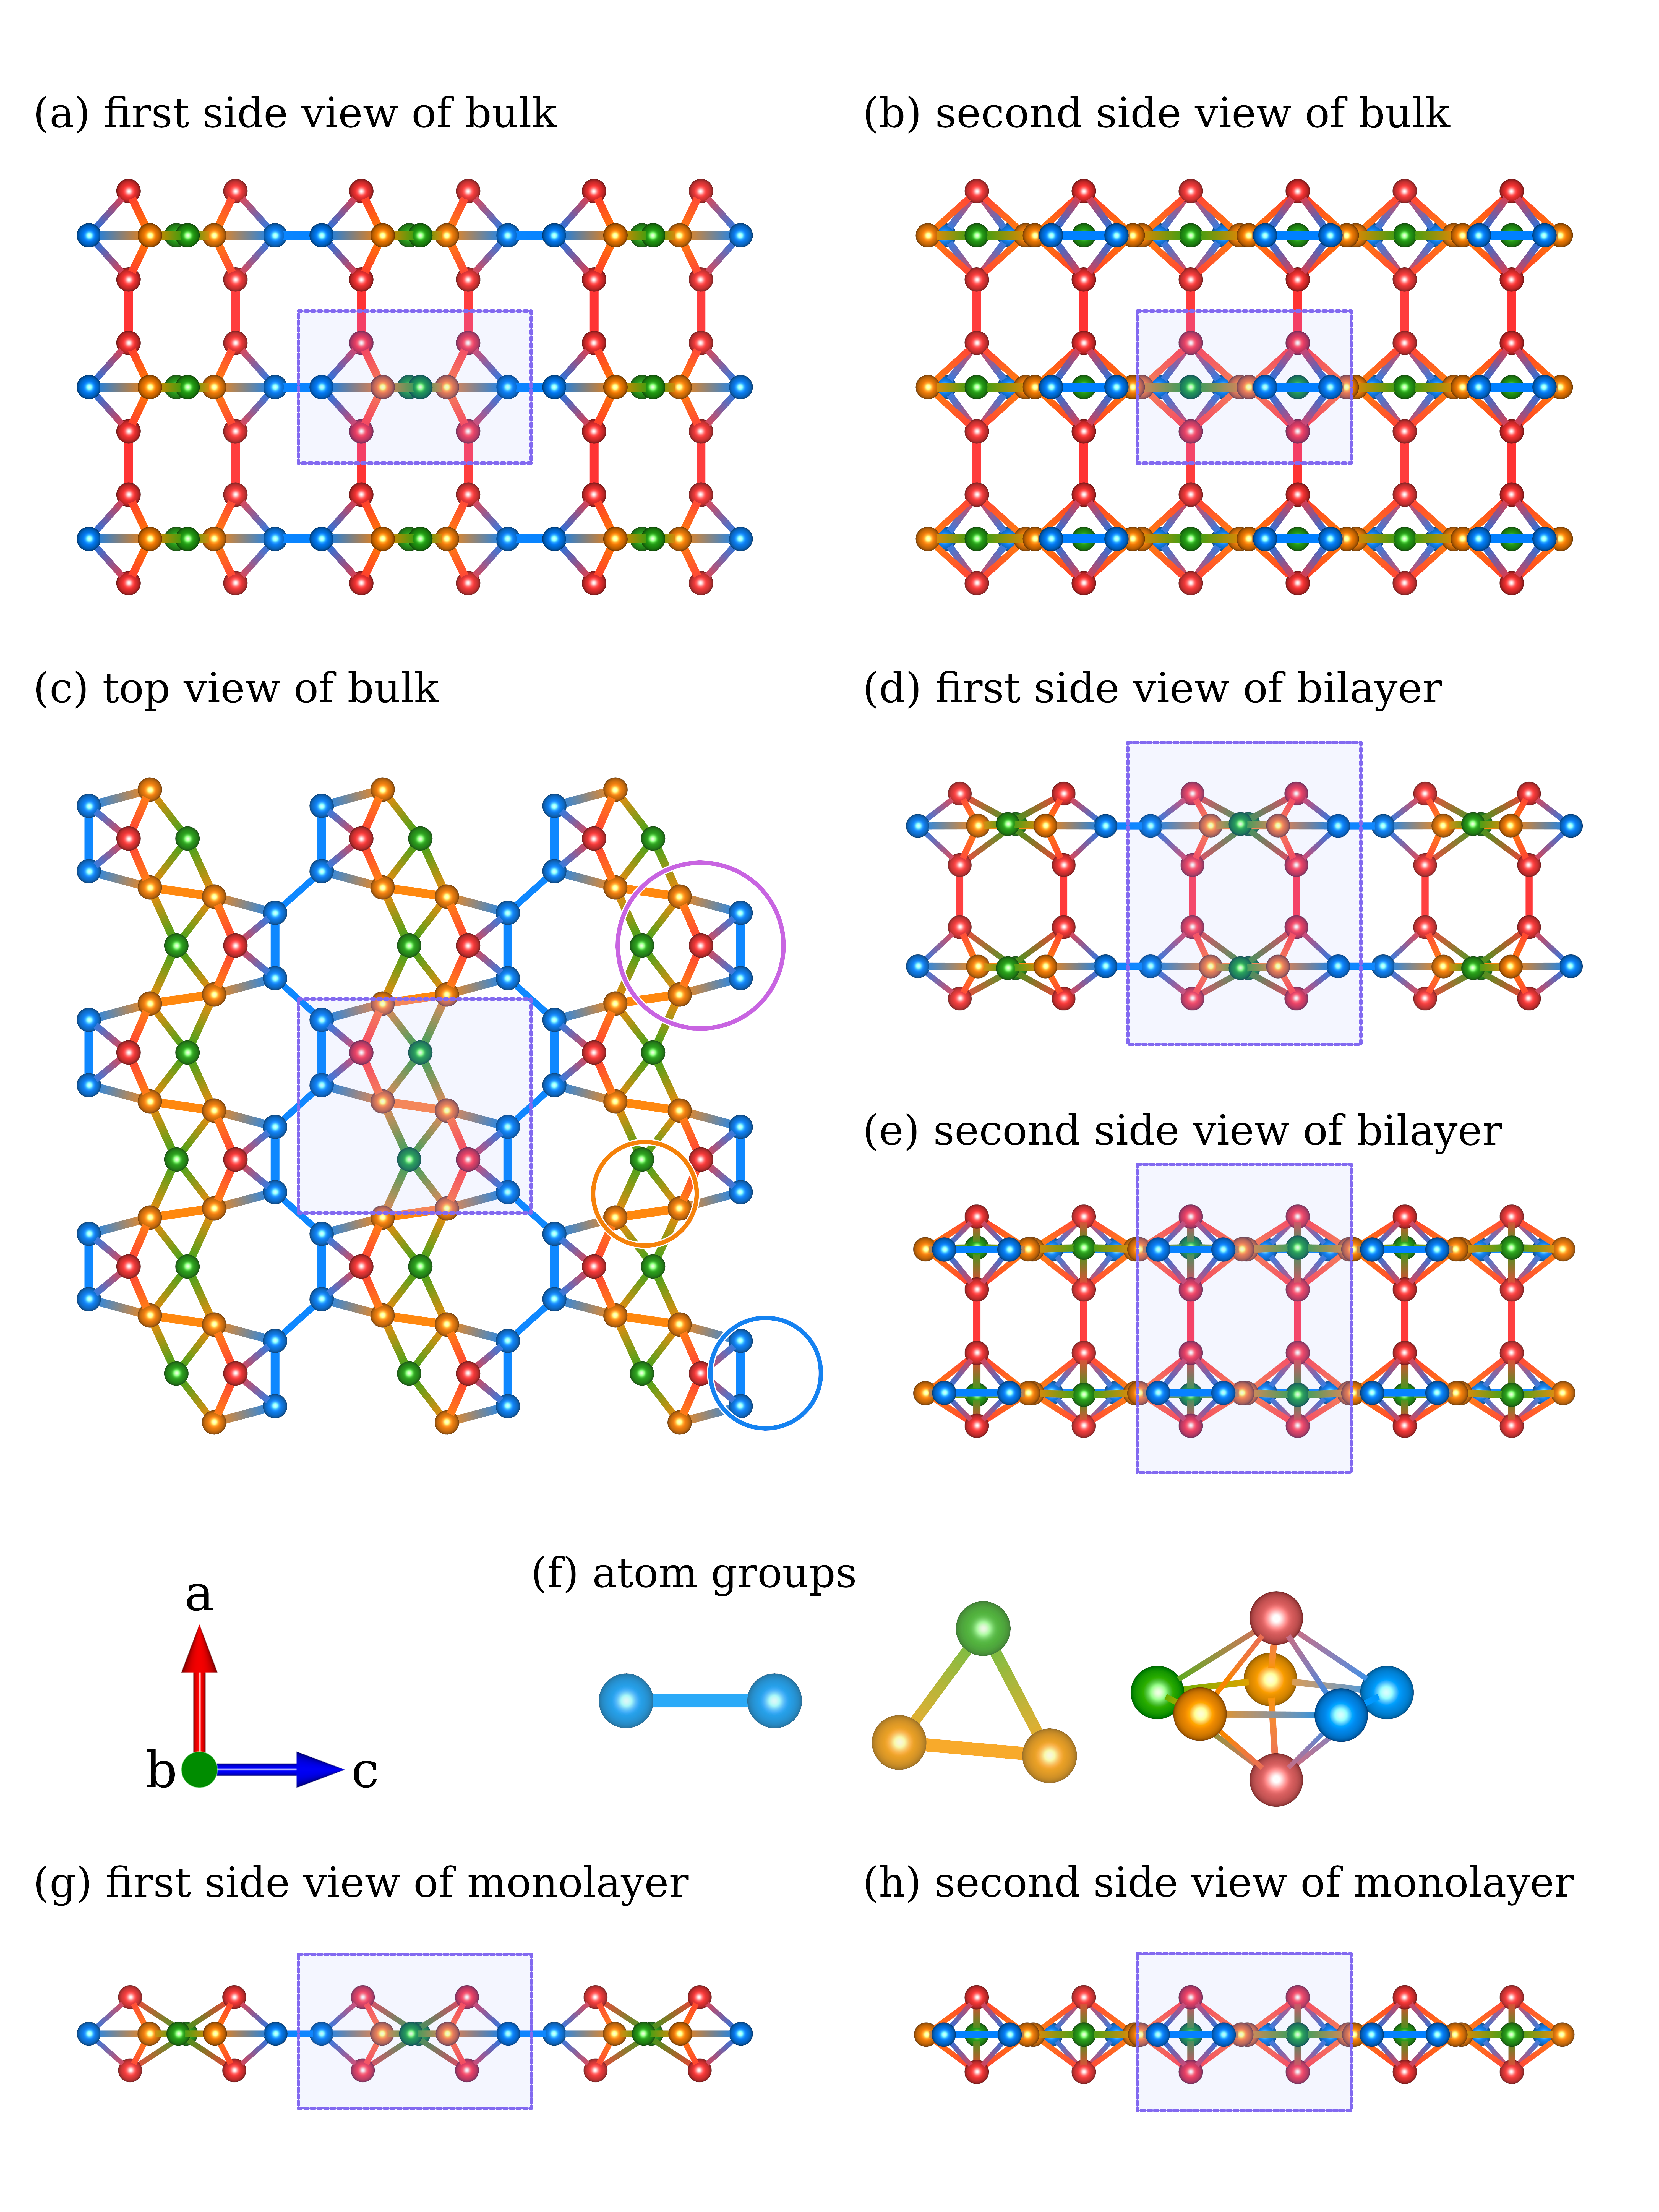
\includegraphics[width=0.80\textwidth]{figures_proj2/fig2.1/fig2.1_6k.png}
\caption{Atomic structure of o-\ce{B14}.
Panels~(a) and~(b) show two side views of the bulk structure,
and panel~(c) shows the corresponding top view.
The boron atoms are grouped into G2 (circled in blue),
G3 (circled in orange), and G7 (circled in purple),
as indicated by the coloured circles in panel~(c) and sketched in panel~(f).
These groups correspond to the two-atom, three-atom, and seven-atom groups used in the bonding analysis, respectively.
Panels~(d) and~(e) show two side views of the bilayer structure.
Panels~(g) and~(h) show two side views of the monolayer structure.}
\label{fig:ob14_atomic_structure}
\end{figure}

This orthorhombic o-\ce{B14} structure is a particularly promising candidate for further investigation,
as it introduces the pentagonal \ce{B7} bipyramidal motif as a fundamental structural unit in crystalline boron,
which differs markedly from the \ce{B12} icosahedral units that dominate most known boron phases.
This unusual topology leads to highly delocalized multicentre bonding,
including the predicted seven-centre-two-electron $\pi$ bonds,
suggesting that the electronic structure may host unconventional features such as anisotropic transport, unusual phonon behaviour,
and potentially strong electron-phonon coupling.
Since the phase is predicted to be dynamically stable at ambient pressure, \textit{ab initio} studies of
its electronic band structure, phonon spectrum, and superconducting properties would be valuable,
as would studies that explore how the unique bipyramidal building blocks influence the broader physics of electron-deficient boron networks.
Moreover, this also raises the question of whether it may be stable in two-dimensional form,
where the interlayer connectivity consists only of single B-B bonds.

In this chapter, we use density functional theory calculations to investigate the electronic and optical properties of bulk o-\ce{B14} and its monolayer and bilayer forms.
Hydrogen termination of the two-dimensional structures is also considered.
Interestingly, bilayer o-\ce{B14} is found to be a semiconductor with a band gap of around
\qty{0.67}{\electronvolt} as calculated using the HSE06 hybrid functional.
The hydrogen-terminated bilayer, however, is predicted to support phonon-mediated superconductivity,
while monolayer o-\ce{B14} is found to be magnetic.
The optical properties reveal distinctive anisotropic behaviour and energy-loss features consistent with plasmon resonances in the near-infrared to mid-infrared range for in-plane excitation,
as well as the ultraviolet energy range for out-of-plane excitation,
broadening the potential of boron for applications in optoelectronics, plasmonics, and catalysis.

This chapter is organized as follows.
Section~\ref{2_methods} presents the computational methods.
Then, section~\ref{2_results} discusses the electronic, superconducting, and optical properties.
Finally, section~\ref{2_conclusions} gives the conclusions.

\FloatBarrier
\section{Computation methods}
\label{2_methods}

The density functional theory calculations are performed using the Vienna Ab initio Simulation Package, \texttt{VASP}~\cite{kresse1993ab,kresse1994ab,kresse1996efficiency,kresse1996efficient}.
The projector augmented wave method is used to describe the electron-ion interactions~\cite{kresse1999ultrasoft}.
The generalized gradient approximation of Perdew--Burke--Ernzerhof is employed for the exchange-correlation functional~\cite{perdew1996generalized},
along with the D3 dispersion correction with Becke--Johnson damping to account for long-range van der Waals interactions~\cite{becke2005density,grimme2010consistent,grimme2011effect}.
For bulk o-\ce{B14}, a $\Gamma$-centred k-point mesh of $34 \times 48 \times 31$ is used with a plane-wave energy cutoff of \qty{600}{\electronvolt}.
The electronic convergence criterion is set to \qty{1e-6}{\electronvolt},
and the structures are relaxed until all forces on each atom are below \qty{0.01}{\electronvolt\per\angstrom}.
For the two-dimensional systems, a vacuum region of approximately \qty{22}{\angstrom} is included,
and a k-point mesh of $20 \times 18 \times 1$ is used.
Convergence tests show that these settings yield accurate results,
as shown in figures~\ref{S2.1}--\ref{S2.3} of the Supplementary Information.

For selected calculations,
we also use the screened hybrid exchange-correlation functional of Heyd, Scuseria, and Ernzerhof, HSE06,
which can improve band-gap estimates relative to semilocal functionals~\cite{sassnick2021electronic,krukau2006influence}.
Unless explicitly stated otherwise,
all figures show results obtained using the Perdew--Burke--Ernzerhof functional.
For the density-of-states calculations for bulk o-\ce{B14},
we use a $\Gamma$-centred k-point mesh of $20 \times 28 \times 18$.
For the two-dimensional systems,
we use a mesh of $20 \times 18 \times 1$.
The Fermi-level smearing is calculated using the Gaussian method with a broadening value of \qty{0.1}{\electronvolt}.
For the spin-resolved HSE06 monolayer spectra in figure~\ref{S2.16},
we reconstruct the total DoS from the archived eigenvalues and k-point weights on a common energy grid,
using a Gaussian broadening of \qty{0.05}{\electronvolt}.

For hydrogen termination,
the hydrogen atoms are placed on top of the boron atoms of the bipyramids.
The hollow-bridge site,
located between the two apical boron atoms on each side of the layer,
is also considered for comparison,
as shown in figure~\ref{S2.7}.

The adsorption energy per atom, $E_{\mathrm{ad}}$, of hydrogen atoms on the surface is calculated as:

\begin{equation}
    E_{\mathrm{ad}} = \frac{E_{\mathrm{H/B}} - E_{\mathrm{B}} - n_{\mathrm{H}}E_{\mathrm{H}}}{n_{\mathrm{H}}}
\label{hydrogen_adsorption_energy}
\end{equation}

here, $E_{\mathrm{H/B}}$ is the total energy of the adsorption system,
$E_{\mathrm{B}}$ represents the total energy of the pristine two-dimensional boron structure,
$E_{\mathrm{H}}=E_{\ce{H2}}/2$ denotes half the total energy of an isolated \ce{H2} molecule,
and $n_{\mathrm{H}}$ denotes the number of hydrogen atoms in the unit cell.
We evaluate all adsorption energies from non-spin-polarized total energies.

The cohesive energy per atom, $E_{\mathrm{c}}$, of the boron systems is calculated as:

\begin{equation}
    E_{\mathrm{c}}
    = \frac{E_{\mathrm{B\text{-}struc}} - n_{\mathrm{B}}E_{\mathrm{B\text{-}atom}}}{n_{\mathrm{B}}}
\label{cohesive_energy_per_atom}
\end{equation}

here,
$E_{\mathrm{B\text{-}struc}}$ represents the total energy of the boron structure of interest,
$E_{\mathrm{B\text{-}atom}}$ is the total energy of a free boron atom calculated in a large supercell,
and $n_{\mathrm{B}}$ denotes the number of boron atoms in the unit cell of the structure.
We evaluate all cohesive energies without the dispersion correction.

The charge-density difference, $\Delta \rho(\vec{r}\,)$, for hydrogen adsorption on the surface is calculated as:

\begin{equation}
    \Delta \rho(\vec{r}\,) =
    \rho_{\mathrm{H/B}}(\vec{r}\,)
    - \rho_{\mathrm{B}}(\vec{r}\,)
    - \rho_{\mathrm{H}}(\vec{r}\,)
\label{charge_density_difference_hydrogen_adsorption}
\end{equation}

here, $\rho_{\mathrm{H/B}}(\vec{r}\,)$ is the total charge density of the adsorbed system,
and $\rho_{\mathrm{B}}(\vec{r}\,)$ and $\rho_{\mathrm{H}}(\vec{r}\,)$ are the charge densities of the boron and hydrogen fragments,
respectively.
Both fragments are evaluated in the same cell and at the atomic positions of the adsorption system;
the hydrogen fragment contains all the adsorbed hydrogen atoms.

The dynamical stability of the pristine monolayer and bilayer,
as well as the hydrogen-terminated structures,
is examined from the phonon-dispersion curves using the finite-difference method.
The main phonon dispersions are calculated using $(3\times3)$ supercells.
The comparison with $(2\times2)$ supercells is included in figures~\ref{S2.8} and~\ref{S2.9}.
For the hydrogen-terminated bilayer,
\textit{ab initio} molecular dynamics calculations are also carried out using \texttt{VASP} in the NVT ensemble at \qty{400}{K}.
A Nosé--Hoover thermostat, a time step of \qty{1}{fs},
and a $2\times2$ supercell containing 112 boron and 16 hydrogen atoms are used.
The trajectory extends over \qty{5.5}{ps}, as shown in figure~\ref{S2.10}.

The superconducting behaviour of o-\ce{B14} is investigated systematically in three structural phases,
namely bulk, monolayer, and hydrogen-terminated bilayer.
Calculations are carried out using the Perdew--Burke--Ernzerhof formulation of the generalized gradient approximation~\cite{perdew1996generalized},
as provided in \texttt{Quantum ESPRESSO}~\cite{giannozzi2009quantum}.
Norm-conserving pseudopotentials and a kinetic energy cutoff of $45$~Ry are chosen~\cite{hamann2013optimized},
and a vacuum spacing of \qty{15}{\angstrom} is added for the two-dimensional systems to suppress spurious periodic interactions.
Monkhorst--Pack k-point meshes of $9 \times 12 \times 8$ for the bulk,
$10 \times 10 \times 1$ for the monolayer,
and $9 \times 9 \times 1$ for the bilayer are employed to sample the Brillouin zone~\cite{monkhorst1976special}.
Density functional perturbation theory gives the phonon dispersions and the first-order change in the self-consistent potential
on q-point grids of $3 \times 4 \times 3$,
$5 \times 5 \times 1$, and $3 \times 3 \times 1$, respectively~\cite{baroni2001phonons}.
Atomic positions and lattice parameters are relaxed until residual forces are below $1\times10^{-5}$~Ry/bohr,
corresponding to \qty{2.6e-4}{\electronvolt\per\angstrom}.

Maximally localized Wannier functions are constructed in \texttt{Wannier90} by initializing projections on boron $s$ and $p$ orbitals~\cite{pizzi2020wannier90}.
Uniform k-point meshes of $6 \times 8 \times 6$ for the bulk and $6 \times 6 \times 1$ for the monolayer and bilayer are used in Wannier interpolation.
The localized representation is used to interpolate both the electronic states and the electron-phonon matrix elements,
as defined in equation~\eqref{electron_phonon_matrix_element_method}.
The Fermi-surface average of the squared matrix elements, resolved by phonon frequency,
gives the Eliashberg spectral function $\alpha^2F(\omega)$,
from which $\lambda$ and $\omega_\mathrm{log}$ follow through equation~\eqref{electron_phonon_spectral_moments}.
Superconductivity is subsequently analysed using the \texttt{EPW} code~\cite{giannozzi2009quantum,giannozzi2020quantum,giannozzi2017advanced,ponce2016epw},
which is employed to evaluate the electron-phonon coupling strength and estimate the Allen--Dynes transition temperatures, $T_\mathrm{c}$~\cite{margine2013anisotropic}.
The superconducting properties are also obtained by solving the fully anisotropic Migdal--Eliashberg equations~\cite{bardeen1955electron,giustino2017electron,margine2013anisotropic},
as implemented in the \texttt{EPW} code.
In this treatment, $T_\mathrm{c}$ is obtained from the disappearance of the superconducting gap upon increasing temperature;
it is a separate estimate from the Allen--Dynes result.
The Morel--Anderson pseudopotential $\mu^{*}$ is chosen to be $0.13$,
consistent with the typical semi-empirical range of $0.10$--$0.16$ used in Migdal--Eliashberg calculations for light-element and $sp$-bonded superconductors~\cite{allen-dynes},
and with the value adopted in the literature for boron-based two-dimensional superconductors~\cite{zhao2019two}.
With this choice,
the calculated electron-phonon coupling strengths, $\lambda$, and $T_\mathrm{c}$ indicate clear dimensionality effects,
as discussed in section~\ref{2_superconducting}.

For the calculation of the optical properties within \texttt{VASP},
in particular the frequency-dependent dielectric tensor $\varepsilon_{\alpha\beta}(\omega)$,
the k-point meshes of $20 \times 28 \times 18$ and $20 \times 18 \times 1$ are found to yield converged results for the bulk and two-dimensional systems,
respectively, as shown in figure~\ref{S2.4}.
A convergence check for the total number of bands, including the unoccupied states, is also performed,
as shown in figure~\ref{S2.5} for bulk o-\ce{B14}.
The input value \texttt{NBANDS=128} is used for the optical calculations.
The archived outputs contain 129 bands for the bulk and 168 for each two-dimensional system.
The displayed bulk spectrum uses the finer $34\times48\times31$ k-point mesh.
The optical calculations use non-spin-polarized PBE states,
with Gaussian occupation smearing of \qty{0.01}{\electronvolt} and \texttt{CSHIFT=0.1}~eV.
No separately parameterized Drude term is added.
The latter broadening is a numerical parameter.
The microscopic expression for the dielectric response,
the Kramers--Kronig relation,
and the derived optical quantities are introduced in chapter~\ref{cha:fundamentals_b},
especially sections~\ref{sec:from_electronic_response_to_dielectric_function} and~\ref{sec:from_dielectric_function_to_optical_properties}.

The dielectric tensor contains the combined dielectric response of the two-dimensional material and the vacuum,
so its magnitude depends on the supercell height~\cite{weng2018honeycomb,laturia2018dielectric}.
For the in-plane response, $\varepsilon^{\mathrm{SC}}(\omega)-1$ scales inversely with the supercell height.
We use the following effective-thickness convention to compare the calculated spectra~\cite{yang2021method}:

\begin{equation}
    \varepsilon_{2}^{\mathrm{2D}}(\omega)
    = \frac{d_{\mathrm{SC}}}{d_{\mathrm{2D}}}
    \varepsilon_{2}^{\mathrm{SC}}(\omega)
    \label{dielectric_vacuum_correction_imaginary}
\end{equation}

\begin{equation}
    \varepsilon_{1}^{\mathrm{2D}}(\omega) =
    1 + \frac{d_{\mathrm{SC}}}{d_{\mathrm{2D}}}
    \left[\varepsilon_{1}^{\mathrm{SC}}(\omega)-1\right]
    \label{dielectric_vacuum_correction_real}
\end{equation}

here, $\varepsilon_{i}^{\mathrm{2D}}(\omega)$ and $\varepsilon_{i}^{\mathrm{SC}}(\omega)$,
with $i=1,2$, denote the effective layer and supercell dielectric functions,
respectively, and $d_{\mathrm{SC}}$ is the supercell height perpendicular to the layer.
The thickness $d_{\mathrm{2D}}$ for the monolayer, bilayer,
and hydrogen-terminated bilayer is \qty{5.807}{\angstrom},
\qty{9.412}{\angstrom}, and \qty{11.209}{\angstrom}, respectively.
The thickness is defined in figure~\ref{S2.6}.
The plotted layer spectra retain the same convention for all three diagonal components.
The resulting magnitudes depend on the chosen $d_{\mathrm{2D}}$.
For perpendicular polarization, the electrostatic boundary condition differs from the in-plane case,
so this rescaling gives an effective quantity of the chosen convention.
The derived layer optical quantities are interpreted within this effective-medium convention.
We note that interband transitions presumably coexist with the plasmons and form a broad background.
The coexistence of individual transitions and plasmons in the same energy range leads to coupling between the two types of excitations,
and hence to finite plasmon lifetimes in the presence of interband transitions~\cite{li2017first}.

\section{Results and discussion}
\label{2_results}


\subsection{\texorpdfstring{Bulk o-\ce{B14}: atomic and electronic structure}{Bulk o-B14: atomic and electronic structure}}
\label{2_bulk_atomic_electronic_structure}

The structural and electronic properties of bulk o-\ce{B14} are investigated first.
The atomic structure is shown in figure~\ref{fig:ob14_atomic_structure}.
This boron allotrope has been predicted, on the basis of first-principles calculations,
to be dynamically stable~\cite{han2023superconducting}.
The structural properties are listed in table~\ref{tab:bulk_ob14_structure}.
Following the previous work on this boron allotrope~\cite{han2023superconducting},
the boron atoms in the unit cell are assigned to three groups,
as indicated by the circles in panel~(c) of figure~\ref{fig:ob14_atomic_structure} and sketched in panel~(f).
These groups are denoted as G2, G3, and G7.
This grouping was obtained using the approach of solid-state adaptive natural density partitioning to analyse the multi-centre bonding.
This method combines ideas from Lewis theory and aromaticity.
It was found that, aside from the four normal two-centre-two-electron and the sixteen three-centre-two-electron B-B $\sigma$-bonds,
there are unusual seven-centre-two-electron $\pi$-bonds~\cite{han2023superconducting}.

\begin{table}[!htbp]
\centering
\rowcolors{2}{gray!15}{white}
\setlength{\tabcolsep}{12pt}
\begin{adjustbox}{center,max width=1.0\linewidth}
\begin{tabular}{cccc}
\hline
\rowcolor{gray!25}
lattice parameter & value & atom & internal coordinate \\ \hline
$a$ & \qty{5.6970}{\angstrom}
& B1~(4x) & \texttt{(0.52123, 0.50000, 0.63796)} \\
$b$ & \qty{4.0479}{\angstrom}
& B2~(4j) & \texttt{(0.60090, 0.50000, 0.89991)} \\
$c$ & \qty{6.2042}{\angstrom}
& B3~(4k) & \texttt{(0.75000, 0.79171, 0.72973)} \\
$\alpha=\beta=\gamma$ & $90^\circ$
& B4~(2f) & \texttt{(0.25000, 0.50000, 0.52367)} \\
\hline
\end{tabular}
\end{adjustbox}
\caption{Lattice constants, lattice angles, and internal coordinates of bulk o-\ce{B14}~\cite{han2023superconducting}.}
\label{tab:bulk_ob14_structure}
\end{table}

\begin{figure}[!htbp]
\centering
    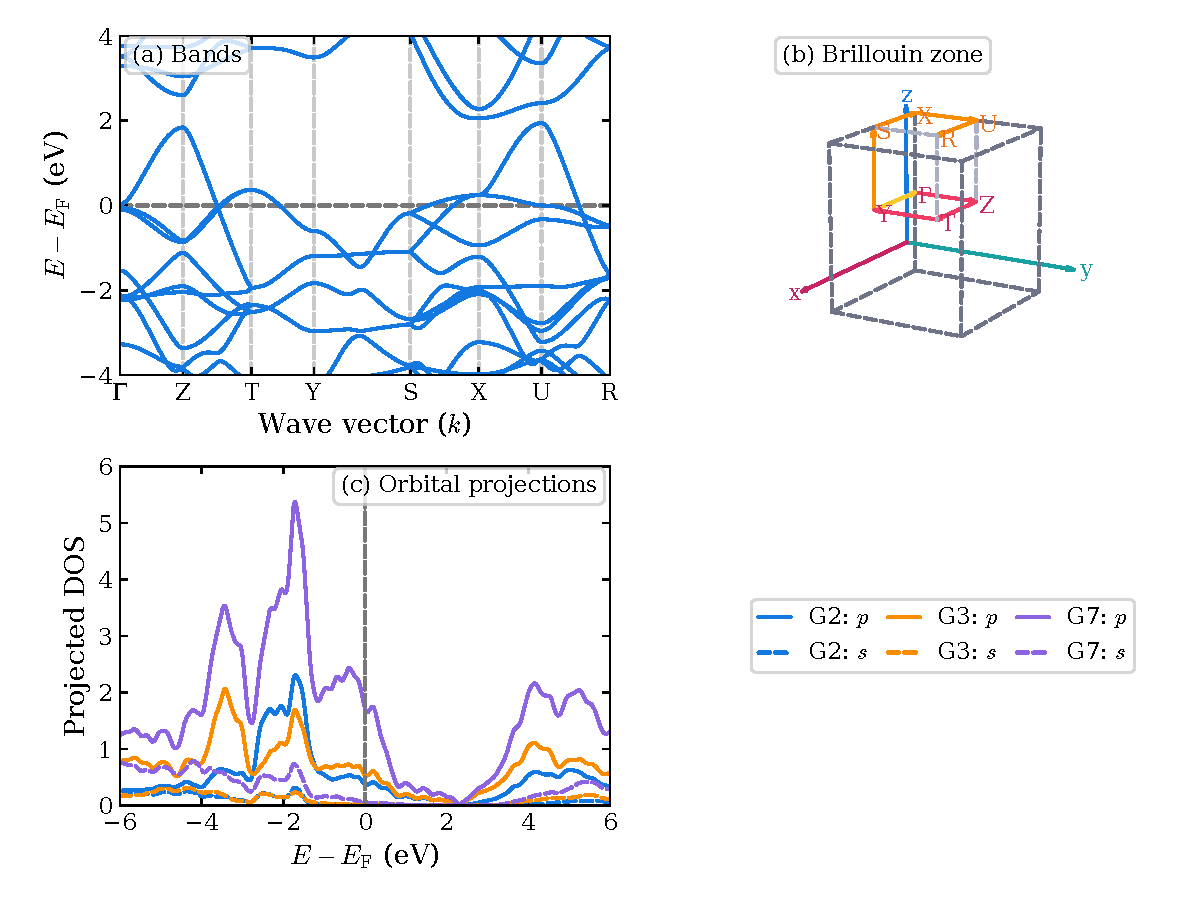
\includegraphics[width=0.80\textwidth]{figures_proj2/fig2.2.pdf}
\caption{Electronic structure of bulk o-\ce{B14}.
The upper-left panel shows the calculated band structure along the selected high-symmetry k-path.
The upper-right panel gives the Brillouin zone together with the corresponding high-symmetry k-path used for the band-structure calculation.
The lower-left panel shows the projected density of states of bulk o-\ce{B14},
resolved into boron $s$ and $p$ orbital contributions for the atom groups defined in panel~(f) of figure~\ref{fig:ob14_atomic_structure}.}
\label{fig:bulk_ob14_band_dos}
\end{figure}

The calculated band structure of bulk o-\ce{B14},
shown in the upper-left panel of figure~\ref{fig:bulk_ob14_band_dos},
exhibits metallic behaviour with three bands crossing the Fermi level.
The corresponding high-symmetry k-path is shown in the upper-right panel.
These bands include steep bands that promote high electron velocities,
as well as flat bands near the Fermi level that enhance the density of states and favour electronic interactions.
Such electronic features suggest the potential for unusual transport and quantum properties.
Furthermore,
the projected density of states shown in the lower-left panel
shows strong orbital hybridization between the boron $2p$ orbitals within the structural units,
which reinforces the stability of the bonding framework.
The calculated cohesive energy of bulk o-\ce{B14} is \qty{-6.16}{\electronvolt}.
Relative to $\alpha$-\ce{B12},
the reported energy difference of o-\ce{B14} is \qty{0.232}{\electronvolt} per atom~\cite{han2023superconducting}.
This positive difference places o-\ce{B14} above $\alpha$-\ce{B12} in energy.

\subsection{\texorpdfstring{Xene o-\ce{B14}: atomic and electronic structure}{Xene o-B14: atomic and electronic structure}}
\label{xene_atomic_electronic_structure}

\subsubsection{Structural properties}
\label{xene_ob14_structural_properties}

The Xene derivatives of o-\ce{B14} are considered next.
The atomic structures of the bilayer and monolayer are shown in panels~(d) and~(e),
and panels~(g) and~(h) of figure~\ref{fig:ob14_atomic_structure},
respectively.
A vacuum region of approximately \qty{22}{\angstrom} in the direction perpendicular to the surface is included.
The hydrogen-terminated bilayer structure is shown in figure~\ref{fig:h_ob14_bilayer_structure},
where the hydrogen atoms are adsorbed on top of the boron atoms of the bipyramids.
We also considered the hollow-bridge site for hydrogen atom adsorption,
located between the two apical boron atoms on each side of the layer,
as shown in figure~\ref{S2.7}.
This adsorption site, however,
is found to be metastable and notably less favourable than the top site,
by \qty{2.62}{\electronvolt} per hydrogen atom for the monolayer
and \qty{2.26}{\electronvolt} per hydrogen atom for the bilayer.

\begin{figure}[!htbp]
\centering
    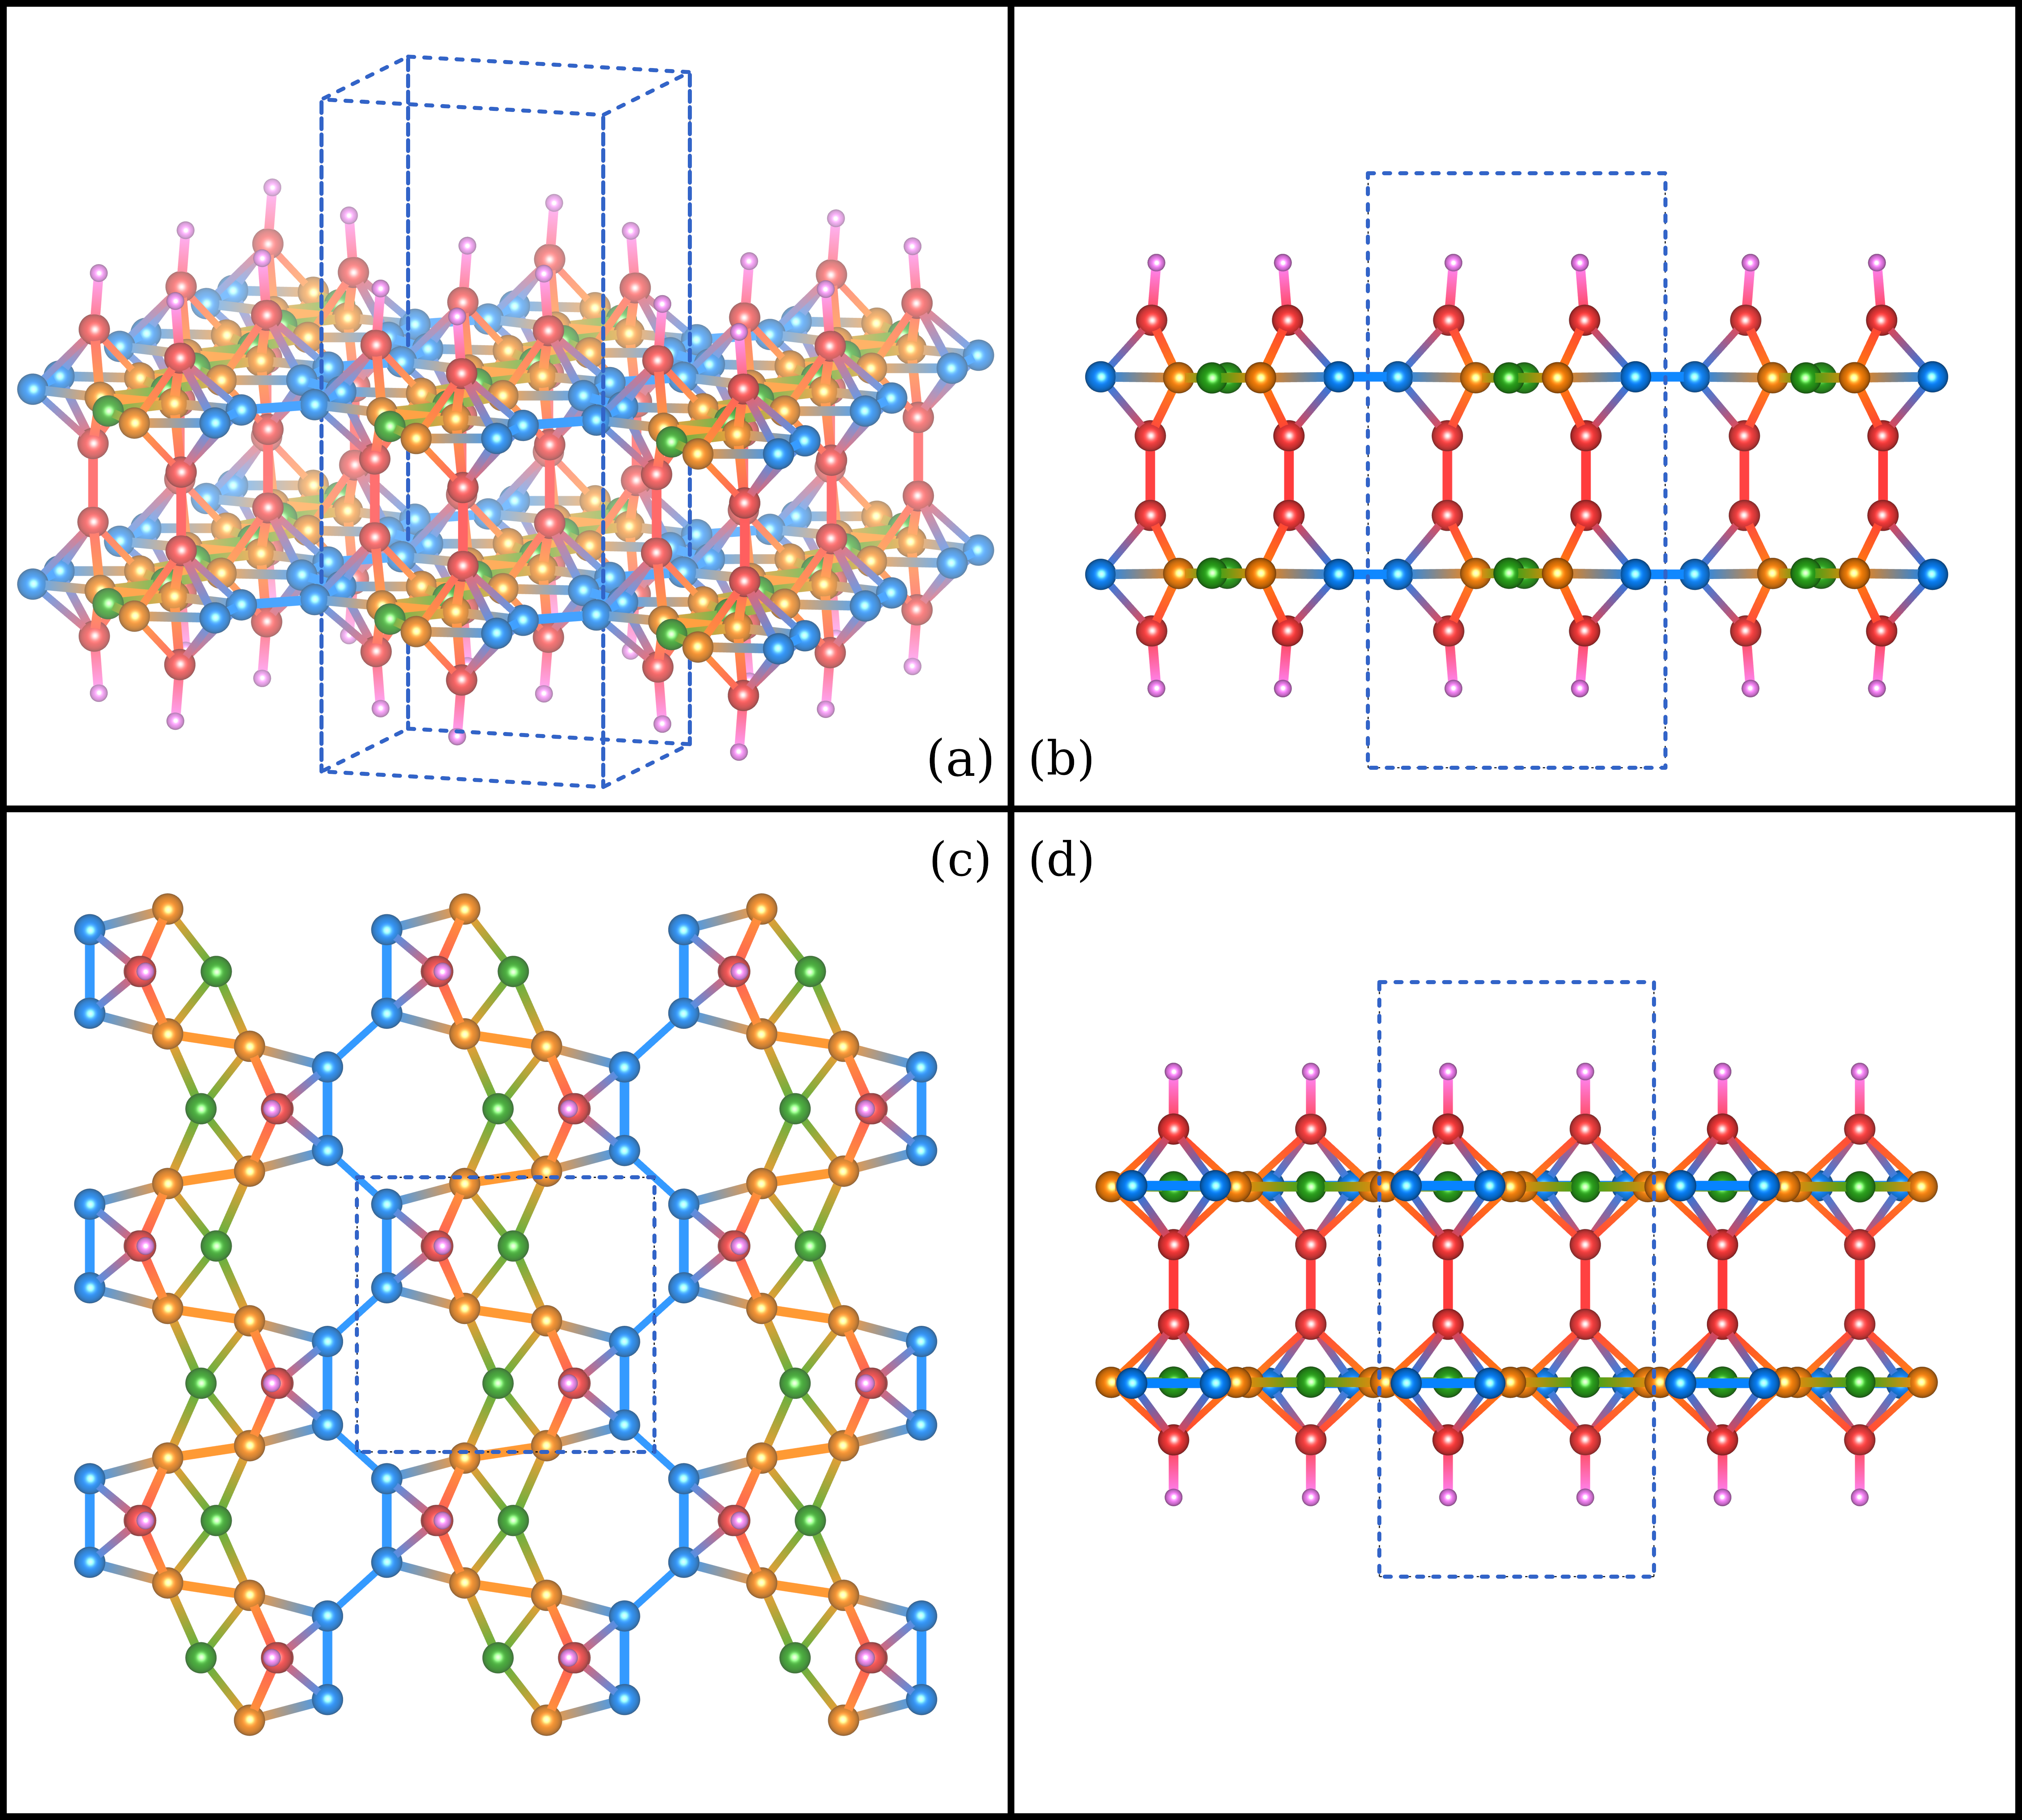
\includegraphics[width=0.80\textwidth]{figures_proj2/fig2.3/fig2.3_4k.png}
\caption{Atomic structure of the hydrogen-terminated bilayer o-\ce{B14}.
Panel~(a) shows the $3\times3$ supercell.
Panels~(b) and~(d) show two side views,
and panel~(c) shows the top view.}
\label{fig:h_ob14_bilayer_structure}
\end{figure}

The optimized structural parameters of the systems are given in table~\ref{tab:xene_ob14_structure},
along with the cohesive energy, adsorption energy, and electronic nature.
Compared with bulk o-\ce{B14},
the in-plane lattice constants of the monolayer and bilayer are slightly larger.
The interlayer B-B distance of the bilayer is also slightly larger than that of the bulk, by about $0.4\%$.
On the other hand,
the in-plane lattice constants of the hydrogen-terminated monolayer and bilayer are slightly smaller compared with the bulk,
and the interlayer B-B distance of the hydrogen-terminated bilayer is reduced by about $2.4\%$.
The cohesive energies of the monolayer and bilayer are \qty{-5.81}{\electronvolt} and \qty{-6.04}{\electronvolt},
respectively.
These values can be compared with \qty{-6.16}{\electronvolt} for bulk o-\ce{B14}
and \qty{-6.00}{\electronvolt} for the $\alpha'$-monolayer,
calculated using the same approach.
The reported adsorption energy per hydrogen atom on the bilayer is \qty{-0.99}{\electronvolt},
which is weaker than that on the monolayer, \qty{-1.45}{\electronvolt}.

\begin{table}[!htbp]
\centering
\rowcolors{2}{gray!15}{white}
\begin{adjustbox}{center,max width=1.0\linewidth}
\begin{tabular}{ccccccc}
\hline
\rowcolor{gray!25}
system
& $a$
& $b$
& \begin{tabular}[c]{@{}c@{}}
interlayer\\B-B (Å)
\end{tabular}
& $E_{\mathrm{c}}$ (eV)
& $E_{\mathrm{ad}}$ (eV)
& electronic nature \\ \hline

monolayer
& 5.700 & 6.314 & - & $-5.81$ & -
&\begin{tabular}[c]{@{}c@{}}
antiferromagnetic\\semiconductor
\end{tabular}\\

H-terminated monolayer
& 5.694 & 6.134 & - & - & $-1.45$ & metallic \\

bilayer
& 5.719 & 6.349 & 1.693 & $-6.04$ & - & semiconductor \\

H-terminated bilayer
& 5.680 & 6.147 & 1.645 & - & $-0.99$ & metallic \\

bulk & 5.697 & 6.204 & 1.686 & $-6.16$ & - & metallic \\

$\alpha'$-monolayer~\cite{niu2024electronic}
& - & - & - & $-6.00$ & - & metallic \\

\hline
\end{tabular}
\end{adjustbox}
\caption{Lattice vectors $a$ and $b$,
interlayer B-B distance,
cohesive energy $E_{\mathrm{c}}$,
adsorption energy $E_{\mathrm{ad}}$,
and electronic nature of the considered o-\ce{B14} systems.
The lattice vectors and interlayer B-B distance are given in \si{\angstrom},
while $E_{\mathrm{c}}$ is given in eV per boron atom and $E_{\mathrm{ad}}$ in eV per hydrogen atom.
For the bulk, $a$ and $b$ denote the lattice constants $a$ and $c$ in table~\ref{tab:bulk_ob14_structure}.
The semiconducting classifications refer to the HSE06 band structures.}
\label{tab:xene_ob14_structure}
\end{table}

\subsubsection{Dynamic stability: phonon dispersion}
\label{xene_ob14_phonon_dispersion}

To investigate whether the monolayer and bilayer structures,
both with and without hydrogen adsorption,
are dynamically stable,
the phonon-dispersion curves are calculated.
The results obtained from finite differences using $3\times3$ supercells are shown in figure~\ref{fig:xene_ob14_phonon_dispersion}
for the monolayer and bilayer.
No imaginary frequencies are present;
therefore,
these two pristine structures are predicted to be dynamically stable.
For the hydrogen-terminated systems,
the monolayer has pronounced imaginary frequencies,
whereas the bilayer has only small imaginary frequencies close to $\Gamma$,
as shown in figures~\ref{S2.8} and~\ref{S2.9}.
These small imaginary frequencies may be sensitive to the numerical treatment of the long-wavelength modes,
but their numerical origin has not been established by the present calculations.
Based on these results,
the hydrogen-terminated monolayer is not considered further.
Using \textit{ab initio} molecular dynamics calculations at a temperature of \qty{400}{K} within \texttt{VASP},
the hydrogen-terminated bilayer retains its bonding framework over the \qty{5.5}{ps} trajectory,
as shown in figure~\ref{S2.10}.
This supports thermal persistence on the simulated time scale.
Together with the cohesive energies and phonon spectra,
it leaves thermodynamic stability against all competing phases and experimental synthesizability as separate questions.

\begin{figure}[!htbp]
\centering
    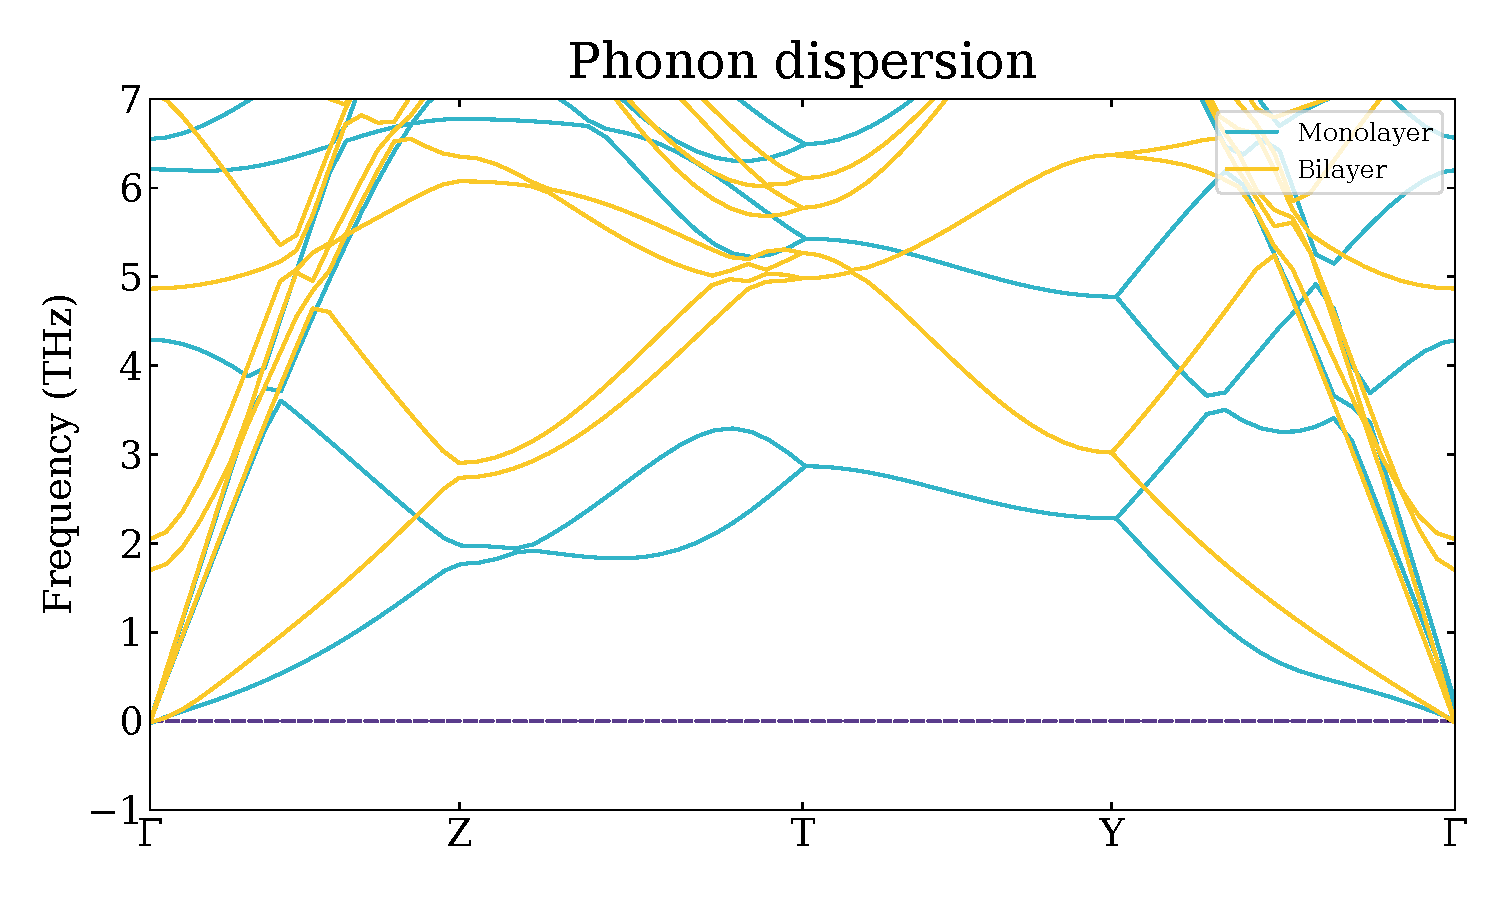
\includegraphics[width=0.60\textwidth]{figures_proj2/fig2.5.pdf}
\caption{Phonon-dispersion curves for monolayer and bilayer o-\ce{B14},
as calculated from finite differences using a $3\times3$ supercell.}
\label{fig:xene_ob14_phonon_dispersion}
\end{figure}

\subsubsection{Electronic properties}
\label{xene_ob14_electronic_properties}

The charge-density difference distribution for hydrogen adsorption on the surface of the bilayer is shown in figure~\ref{fig:h_ob14_charge_density_difference}.
There is a significant depletion of electron density around the hydrogen atoms,
and an increase both in the interlayer B-B bonds and in the $p_z$ orbital of the uppermost bipyramid boron atom.
The latter is directed towards the hydrogen atom and is partially hidden within the large depletion region.
The increase in electron density between the interlayer B-B bond is consistent with the slightly smaller distance compared with the bilayer without hydrogen adsorption.

\begin{figure}[!htbp]
\centering
    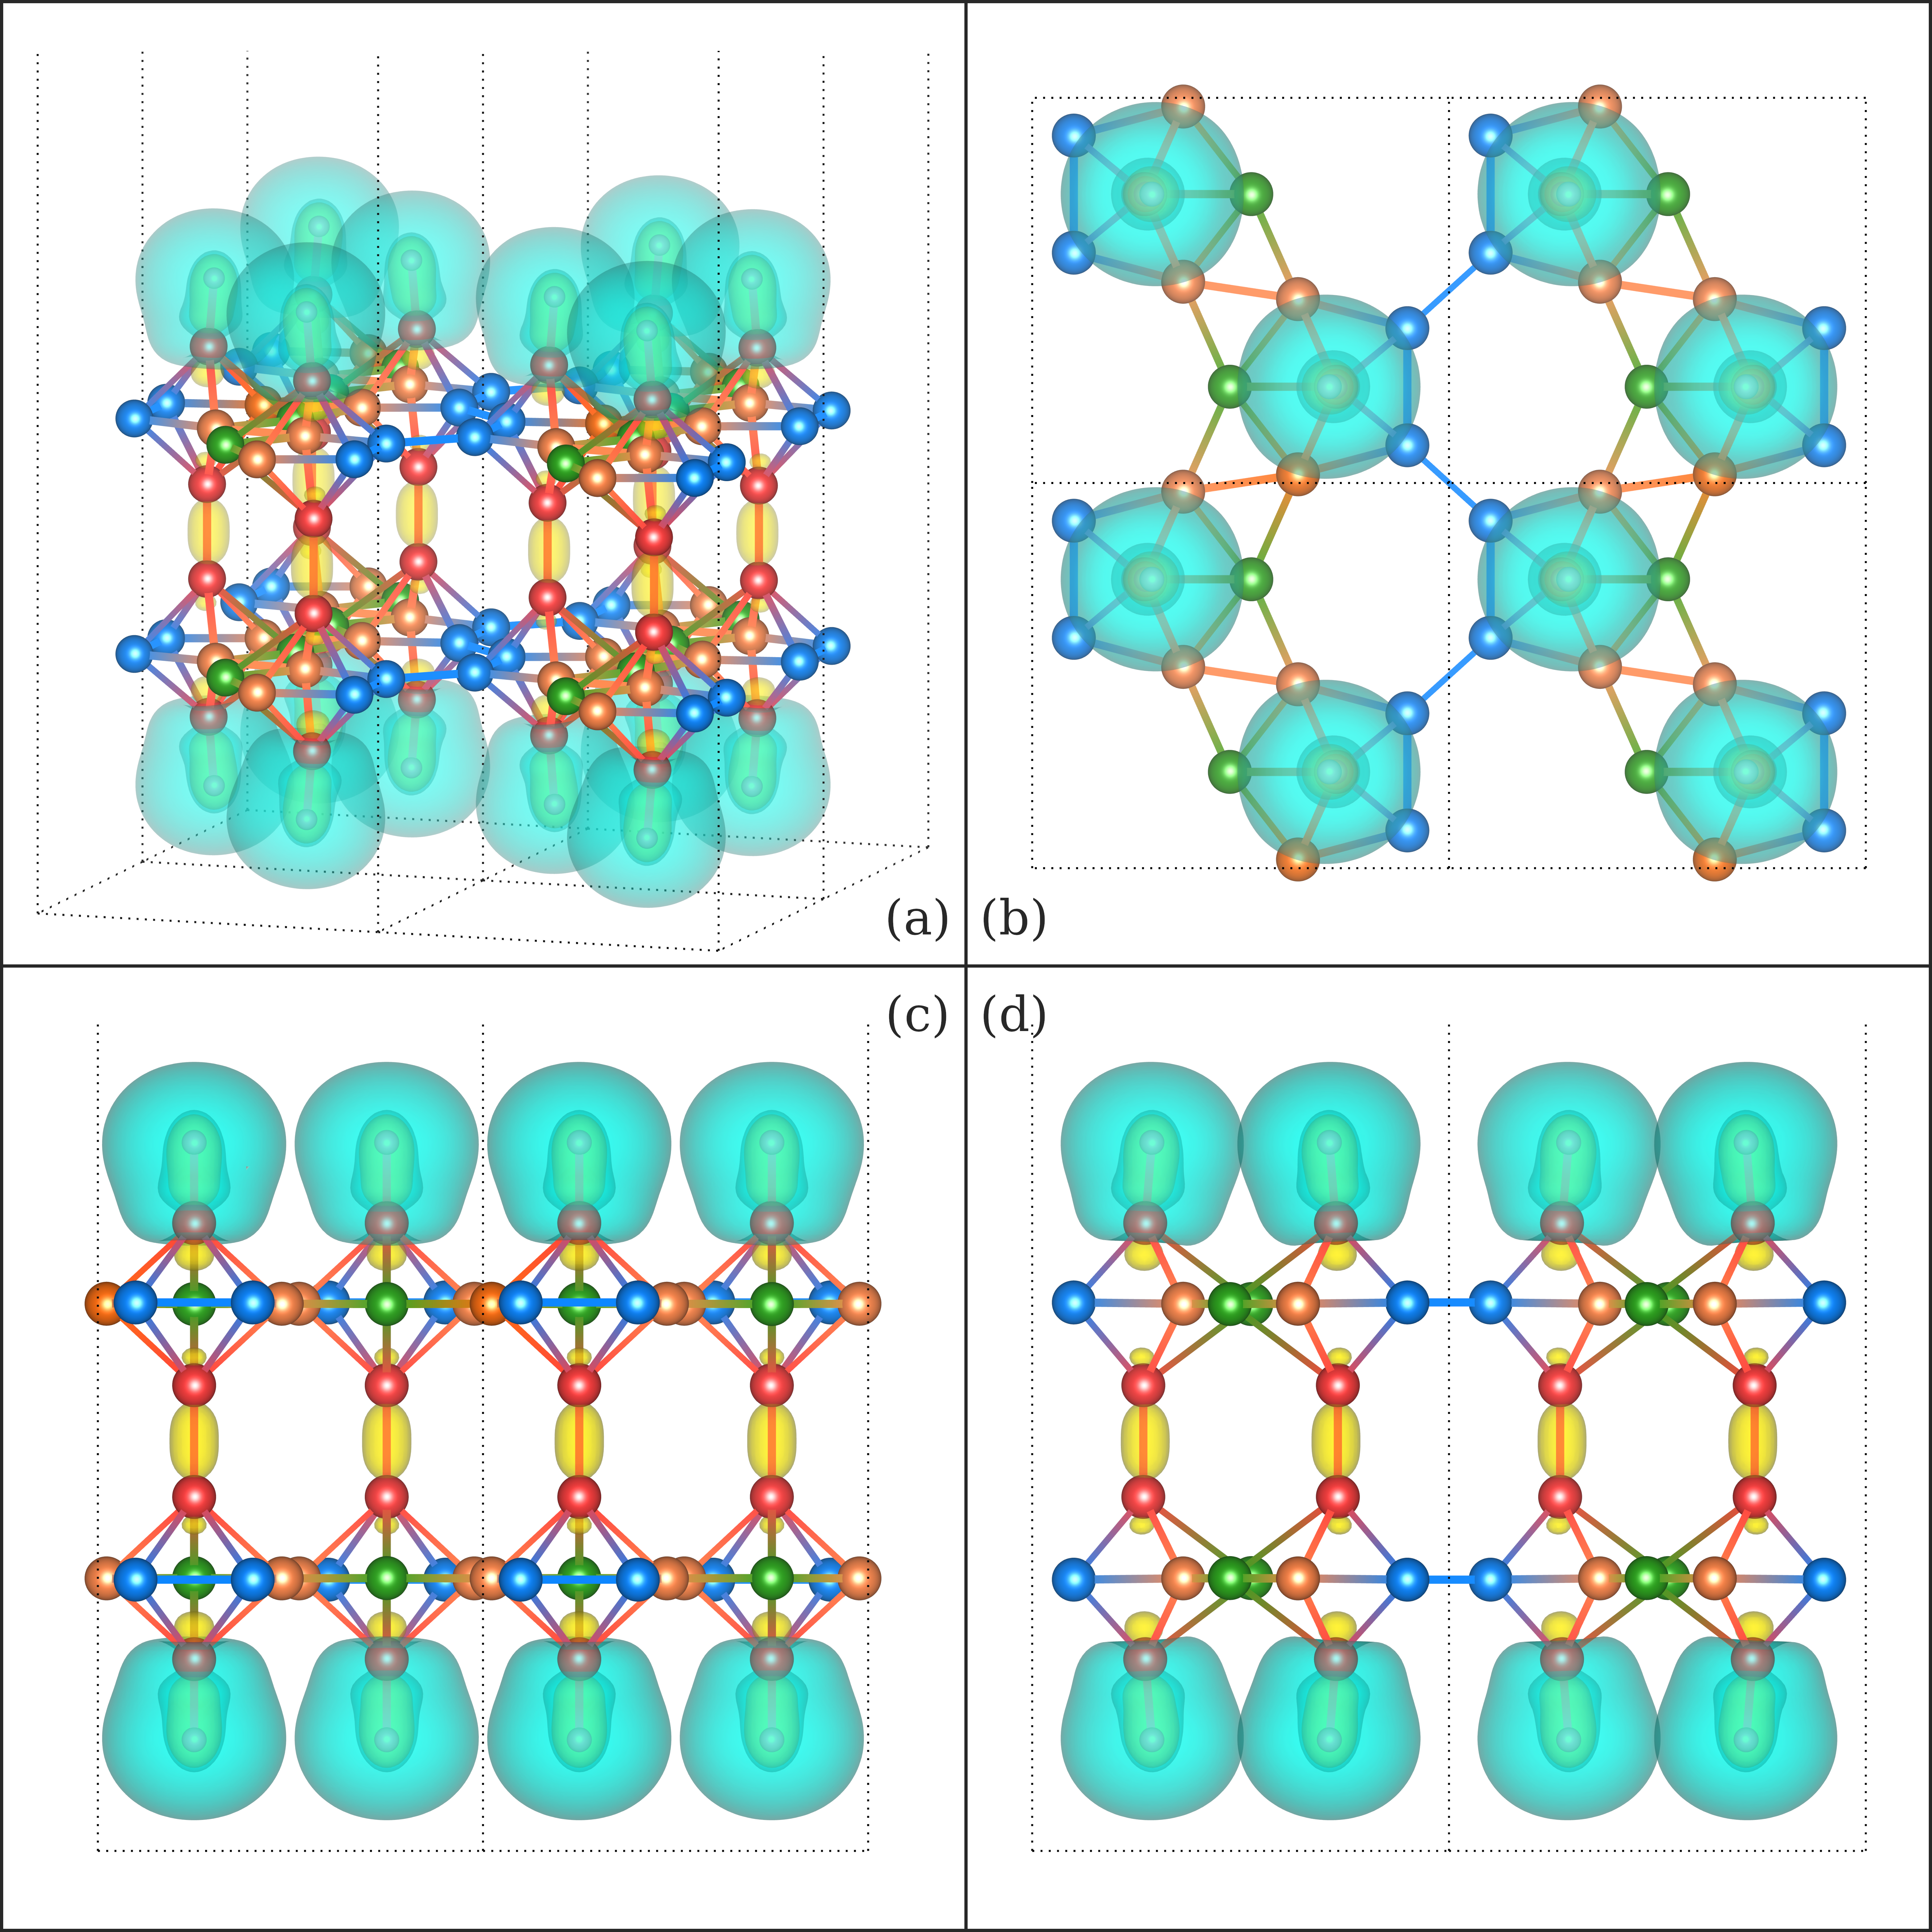
\includegraphics[width=0.80\textwidth]{figures_proj2/fig2.4/fig2.4_6k.png}
\caption{Charge-density difference, $\Delta \rho(\vec{r}\,)$,
for hydrogen adsorption on the bilayer o-\ce{B14} surface.
The charge-density difference is calculated using equation~\eqref{charge_density_difference_hydrogen_adsorption}
for a $2\times2$ supercell.
Regions of charge accumulation are shown in yellow,
and regions of charge depletion are shown in blue.
The isosurface level is $1.5\times10^{-4}~e\,a_0^{-3}$.}
\label{fig:h_ob14_charge_density_difference}
\end{figure}

The spin-polarized band structures of the monolayer are shown in the upper panels of figure~\ref{fig:monolayer_bilayer_band_structure},
as calculated using the HSE06 functional.
In this HSE06 comparison, the antiferromagnetic configuration is lower in energy than the ferromagnetic configuration
by approximately \qty{0.02}{\electronvolt} per 14-atom cell.
This small difference is a zero-temperature energy comparison,
and the magnetic ordering temperature requires a separate calculation.
A small band gap of \qty{0.105}{\electronvolt} opens in the antiferromagnetic case.
In the non-magnetic state,
the system is metallic and exhibits a high density of states at the Fermi level.
This feature is related to flat bands throughout the Brillouin zone,
particularly along the $\mathrm{T}$--$\mathrm{Y}$ direction,
as shown in figures~\ref{S2.12} and~\ref{S2.13}.
Since a large density of states at the Fermi level often suggests that a material is prone to undergo transitions to more stable ground states,
such as forming superconductors, ferromagnets,
or experiencing structural distortions such as the Jahn--Teller effect,
we tested these aspects, as shown in figure~\ref{S2.14}.
The structure is found to be magnetic,
with a magnetic moment of $0.262~\mu_{\mathrm{B}}$ on each apical boron atom.
For the ferromagnetic case,
fixed-spin calculations show a total magnetic moment of around $2~\mu_{\mathrm{B}}$ for the unit cell,
as shown in figure~\ref{S2.15}.
The total density of states of the ferromagnetic structure shows spin splitting,
as shown in the upper panel of figure~\ref{S2.16}.
The corresponding spin-resolved density of states for the antiferromagnetic ordering is shown in the lower panel.

\begin{figure}[!htbp]
\centering
    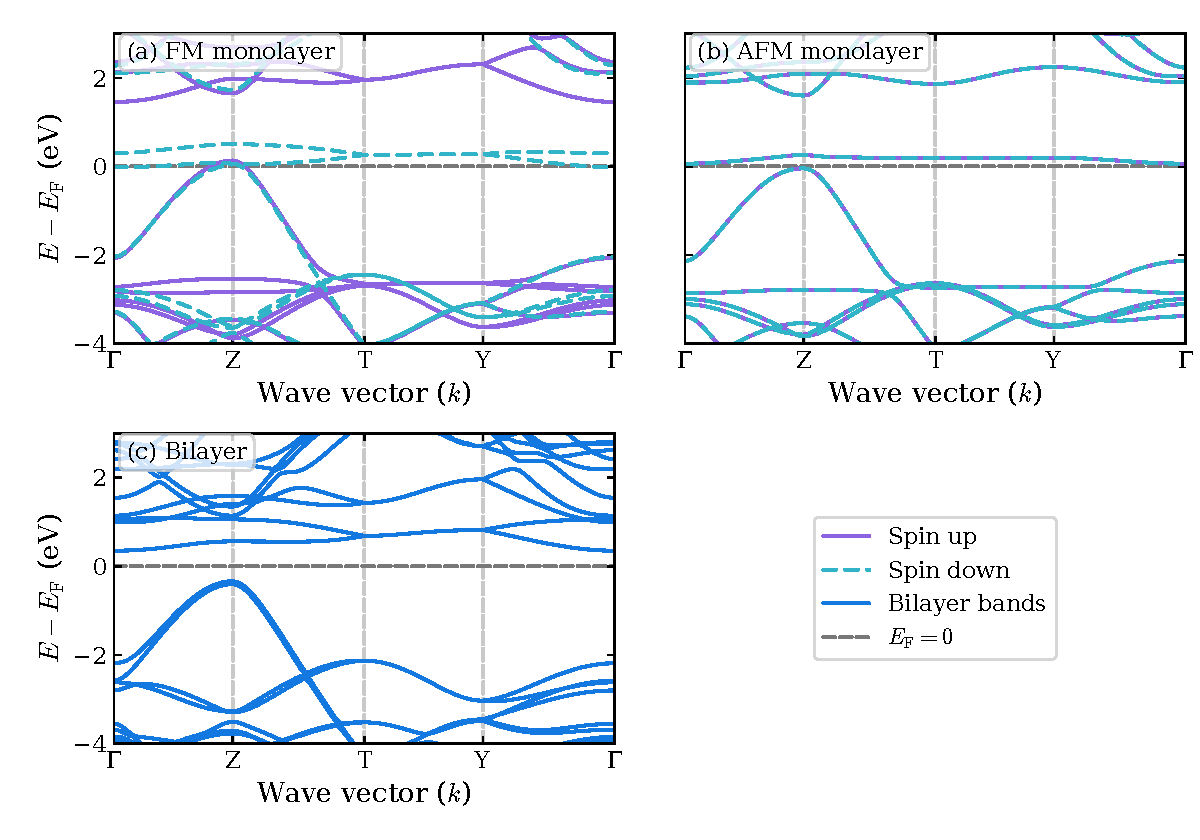
\includegraphics[width=0.80\textwidth]{figures_proj2/fig2.6.pdf}
\caption{Band structures of monolayer and bilayer o-\ce{B14} calculated using the HSE06 functional.
The upper-left and upper-right panels show the spin-polarized ferromagnetic and antiferromagnetic configurations of the monolayer,
respectively.
The lower-left panel shows the band structure of bilayer o-\ce{B14}.}
\label{fig:monolayer_bilayer_band_structure}
\end{figure}

For the antiferromagnetic case,
the spatial distributions of the highest occupied and lowest unoccupied states at a k point midway along the high-symmetry $\mathrm{T}$--$\mathrm{Y}$ direction are shown in figure~\ref{fig:monolayer_afm_states_spin_density}.
The total spin density is also shown in the same figure.
It is apparent that the apical boron atoms of the bipyramid are responsible for the magnetic behaviour of the system,
where they have a magnetic moment of $0.262~\mu_{\mathrm{B}}$.
The analogous result for the ferromagnetic ordering is shown in figure~\ref{S2.17}.
The energetic preference for antiferromagnetic ordering over ferromagnetic ordering can be discussed qualitatively in terms of the competition between electron hopping and exchange interactions.
In the antiferromagnetic configuration,
virtual hopping between neighbouring magnetic sites is enhanced because electrons can delocalize onto oppositely aligned spins without violating the Pauli exclusion principle,
leading to a greater kinetic-energy lowering.
In contrast, ferromagnetic alignment restricts such virtual hopping processes and reduces the associated kinetic-energy gain.
This provides a possible interpretation of the calculated HSE06 ordering.

\begin{figure}[!htbp]
\centering
    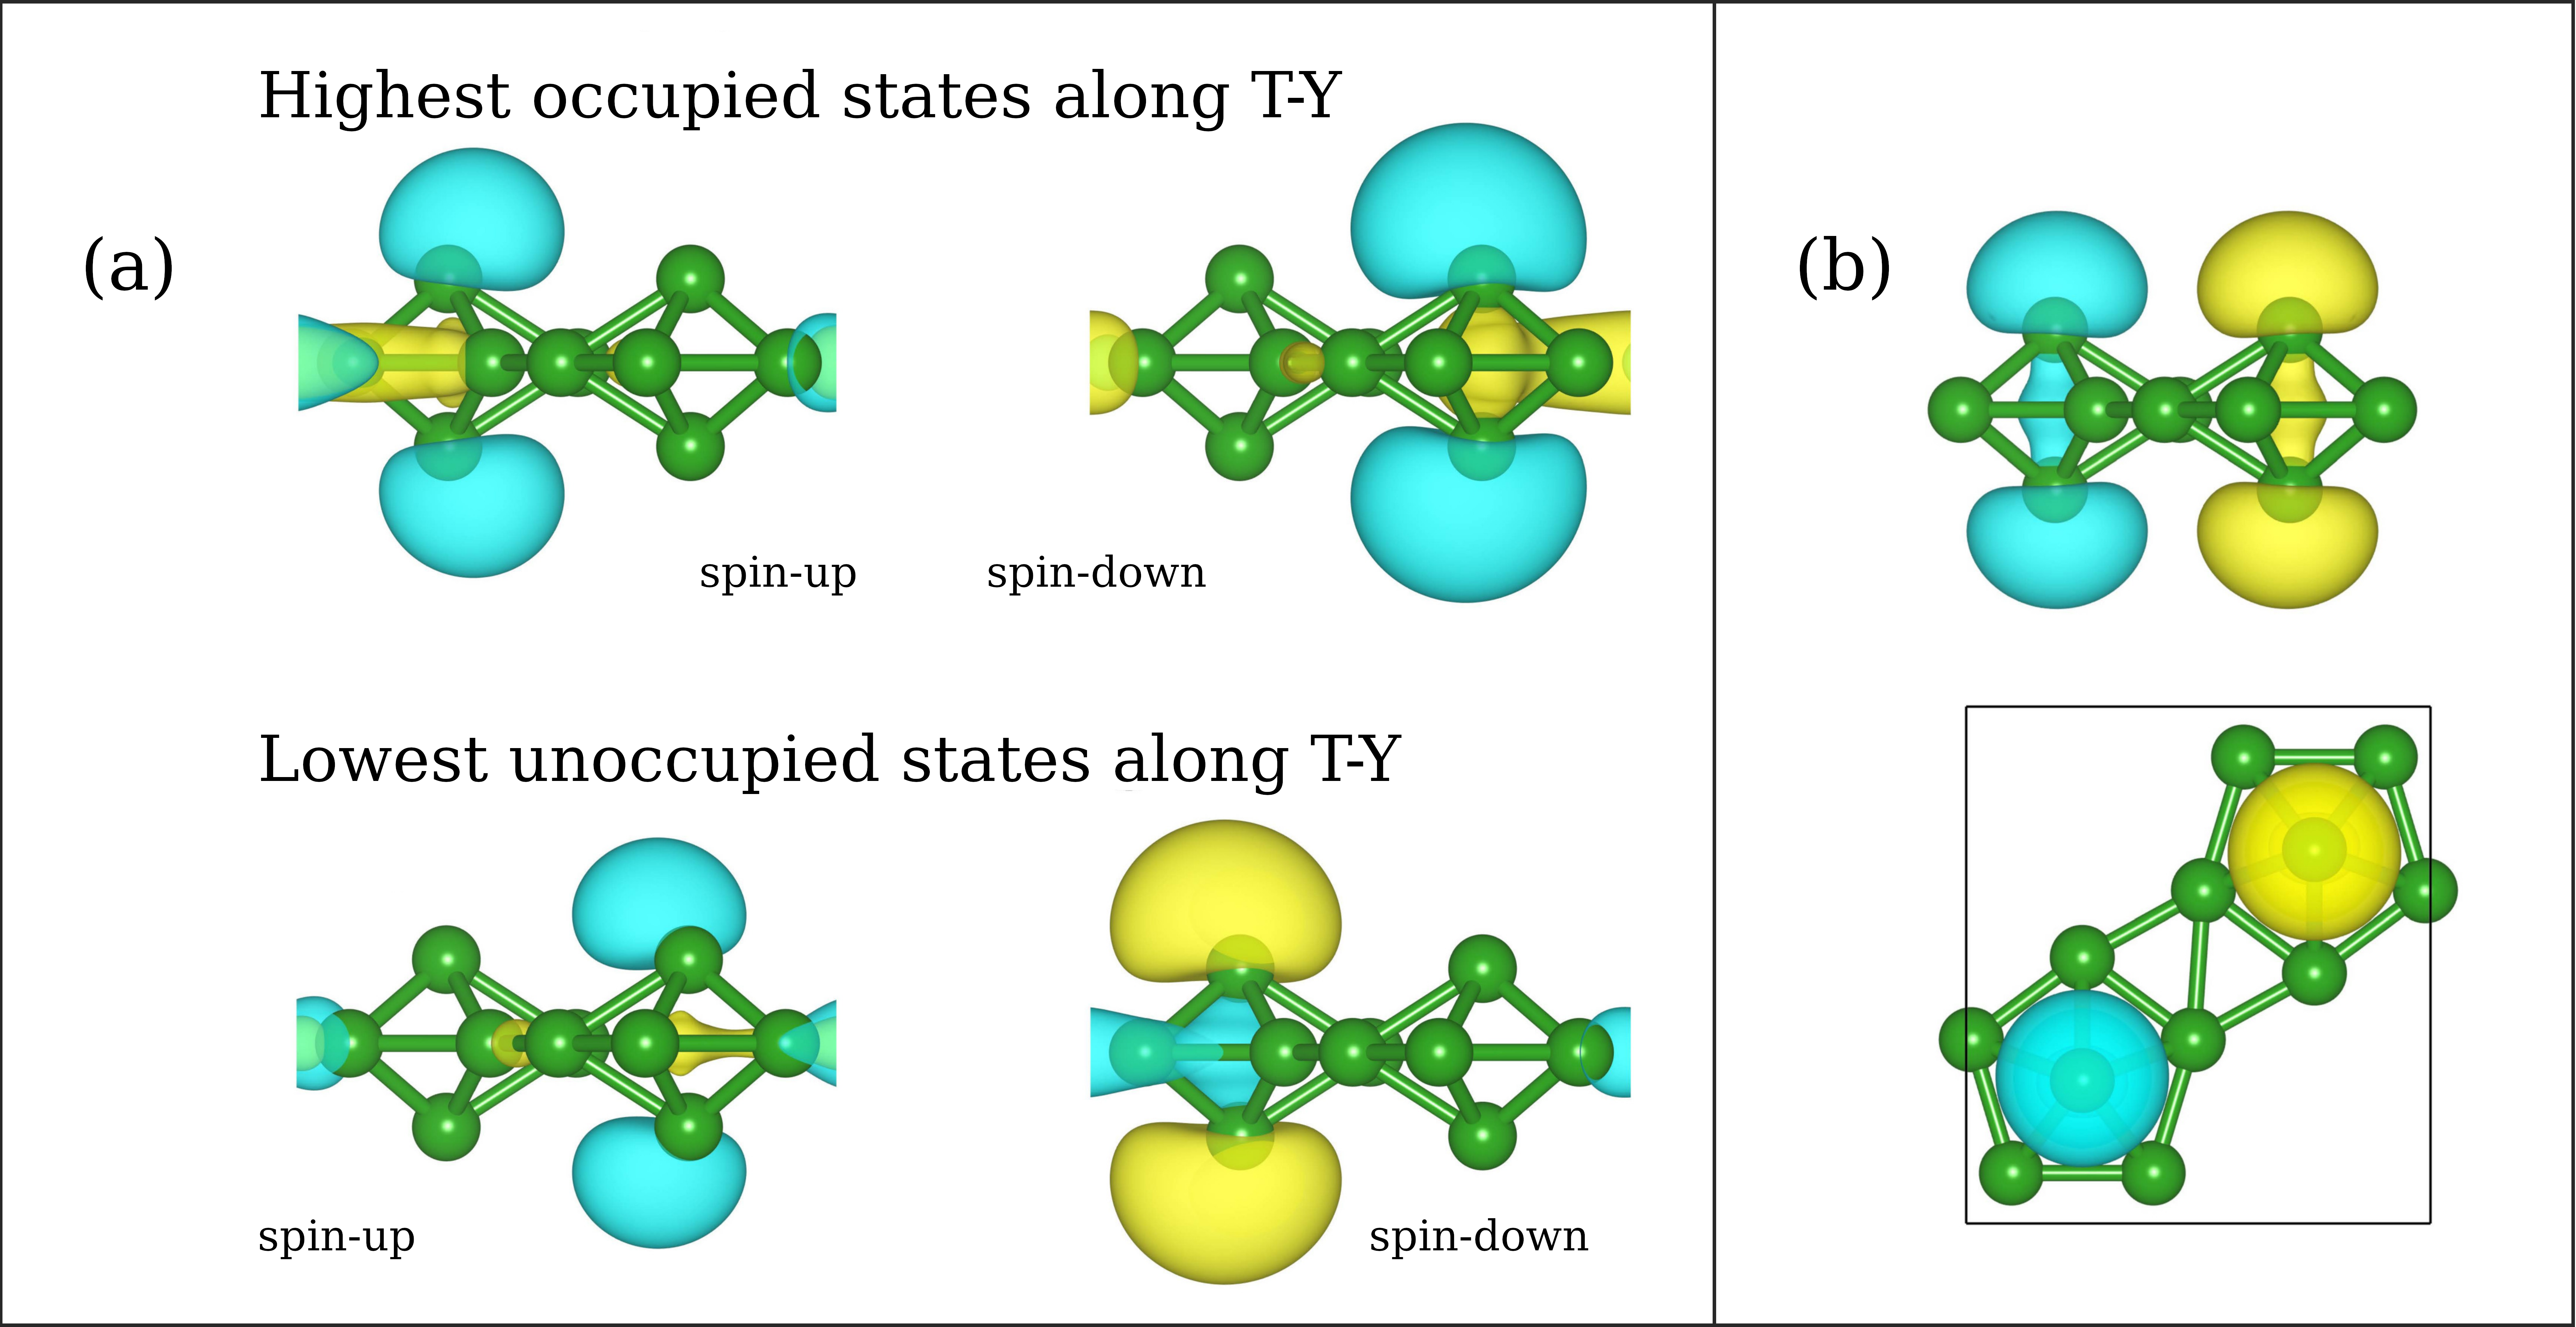
\includegraphics[width=0.80\textwidth]{figures_proj2/fig2.7/fig2.7_from2.6.png}
\caption{Highest occupied and lowest unoccupied spin-up and spin-down states of the monolayer in the antiferromagnetic state
at a k point midway along the high-symmetry $\mathrm{T}$--$\mathrm{Y}$ direction.
The corresponding spin density of the monolayer is also shown.
The isosurface levels are $1\times10^{-7}~e\,\si{\angstrom}^{-3}$ for the state distributions
and $0.005~e\,\si{\angstrom}^{-3}$ for the spin density.}
\label{fig:monolayer_afm_states_spin_density}
\end{figure}

The band structure of the bilayer is shown in the lower-left panel of figure~\ref{fig:monolayer_bilayer_band_structure},
as calculated using the HSE06 functional.
The bilayer is an indirect semiconductor with a band gap of \qty{0.67}{\electronvolt},
where the valence band maximum is at the $\mathrm{Z}$ point and the conduction band minimum is at the $\Gamma$ point.
Using the PBE functional gives a semimetallic band structure.
The screened short-range Fock exchange in HSE06,
as introduced in equation~\eqref{HSE_exchange_correlation_functional},
partly reduces the self-interaction and delocalization errors of semilocal exchange
and changes the relative band-edge energies.
The difference is therefore sensitive to the exchange-correlation approximation,
and both values are theoretical estimates of the gap.
On terminating the bilayer structure with hydrogen,
the band structure changes dramatically.
As shown in figure~\ref{fig:h_bilayer_band_dos},
the hydrogen-terminated bilayer becomes metallic and bears some resemblance to the bulk band structure.

\begin{figure}[!htbp]
\centering
    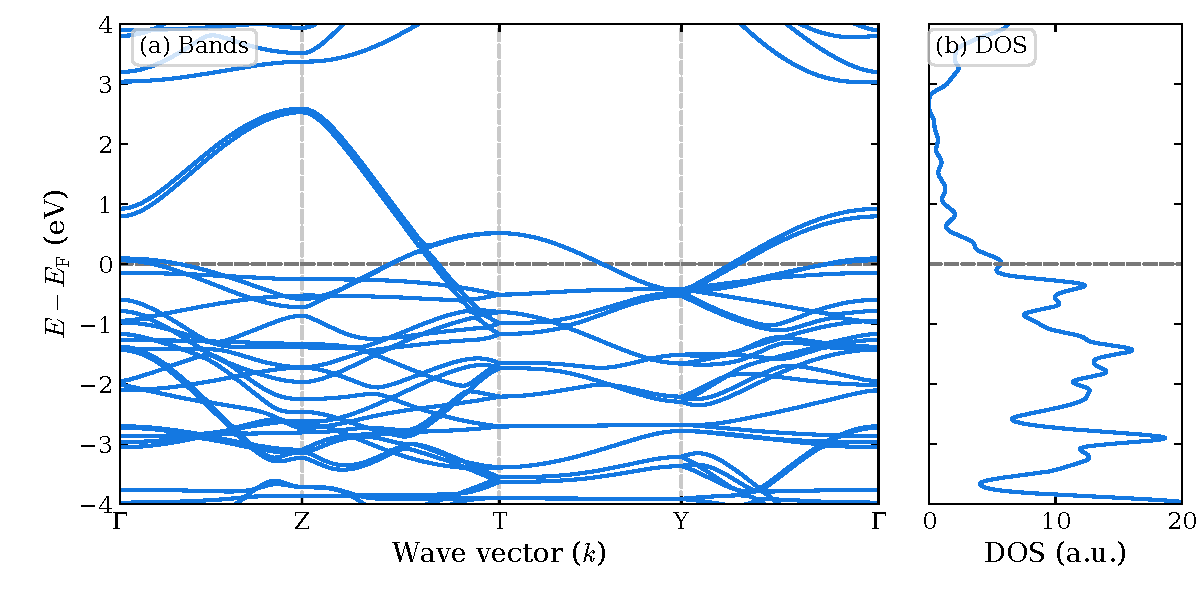
\includegraphics[width=0.80\textwidth]{figures_proj2/fig2.8.pdf}
\caption{Band structure and total density of states of the hydrogen-terminated bilayer o-\ce{B14}.}
\label{fig:h_bilayer_band_dos}
\end{figure}

\subsection{Superconducting properties}
\label{2_superconducting}

The conventional superconducting properties of bulk o-\ce{B14},
the monolayer,
and the hydrogen-terminated bilayer are investigated.
The pristine bilayer is not included in these superconductivity calculations;
its HSE06 band structure is semiconducting.
We first confirm that the atomic relaxation obtained using \texttt{Quantum ESPRESSO} yields very similar results to those obtained using \texttt{VASP}.
For the hydrogen-terminated bilayer,
the lattice constants $a$ and $b$ are \qty{5.66}{\angstrom} and \qty{6.12}{\angstrom} from \texttt{Quantum ESPRESSO},
compared with \qty{5.68}{\angstrom} and \qty{6.14}{\angstrom} from \texttt{VASP}.
The interlayer distance is \qty{4.13}{\angstrom} from \texttt{Quantum ESPRESSO} and \qty{4.11}{\angstrom} from \texttt{VASP},
while the H-B distance is \qty{1.19}{\angstrom} in both cases.

For the bulk phase,
an electron-phonon coupling strength of $\lambda=0.931$ is obtained,
corresponding to an Allen--Dynes superconducting transition temperature of $T_\mathrm{c}=\qty{28.2}{K}$.
This value is consistent with the previously reported value of \qty{29.1}{K}~\cite{han2023superconducting}.
The hydrogen-terminated bilayer exhibits a slightly higher electron-phonon coupling strength,
$\lambda=1.01$,
but a lower transition temperature of $T_\mathrm{c}=\qty{18.5}{K}$.
A larger $\lambda$ can accompany a lower $T_\mathrm{c}$,
since the phonon frequency scale also enters the Allen--Dynes estimate~\cite{migdal1958interaction,marsiglio2020eliashberg,eliashberg1960interactions}.
The reported monolayer coupling, $\lambda=0.05$, is too weak to support an appreciable transition temperature in this calculation.
For $\mu^*=0.13$, it is outside the applicable range of the simplified Allen--Dynes expression in equation~\eqref{allen_dynes_temperature_estimate}.
This result refers to the non-magnetic PBE reference state, separate from the gapped antiferromagnetic HSE06 state.

\begin{figure}[!htbp]
\centering
    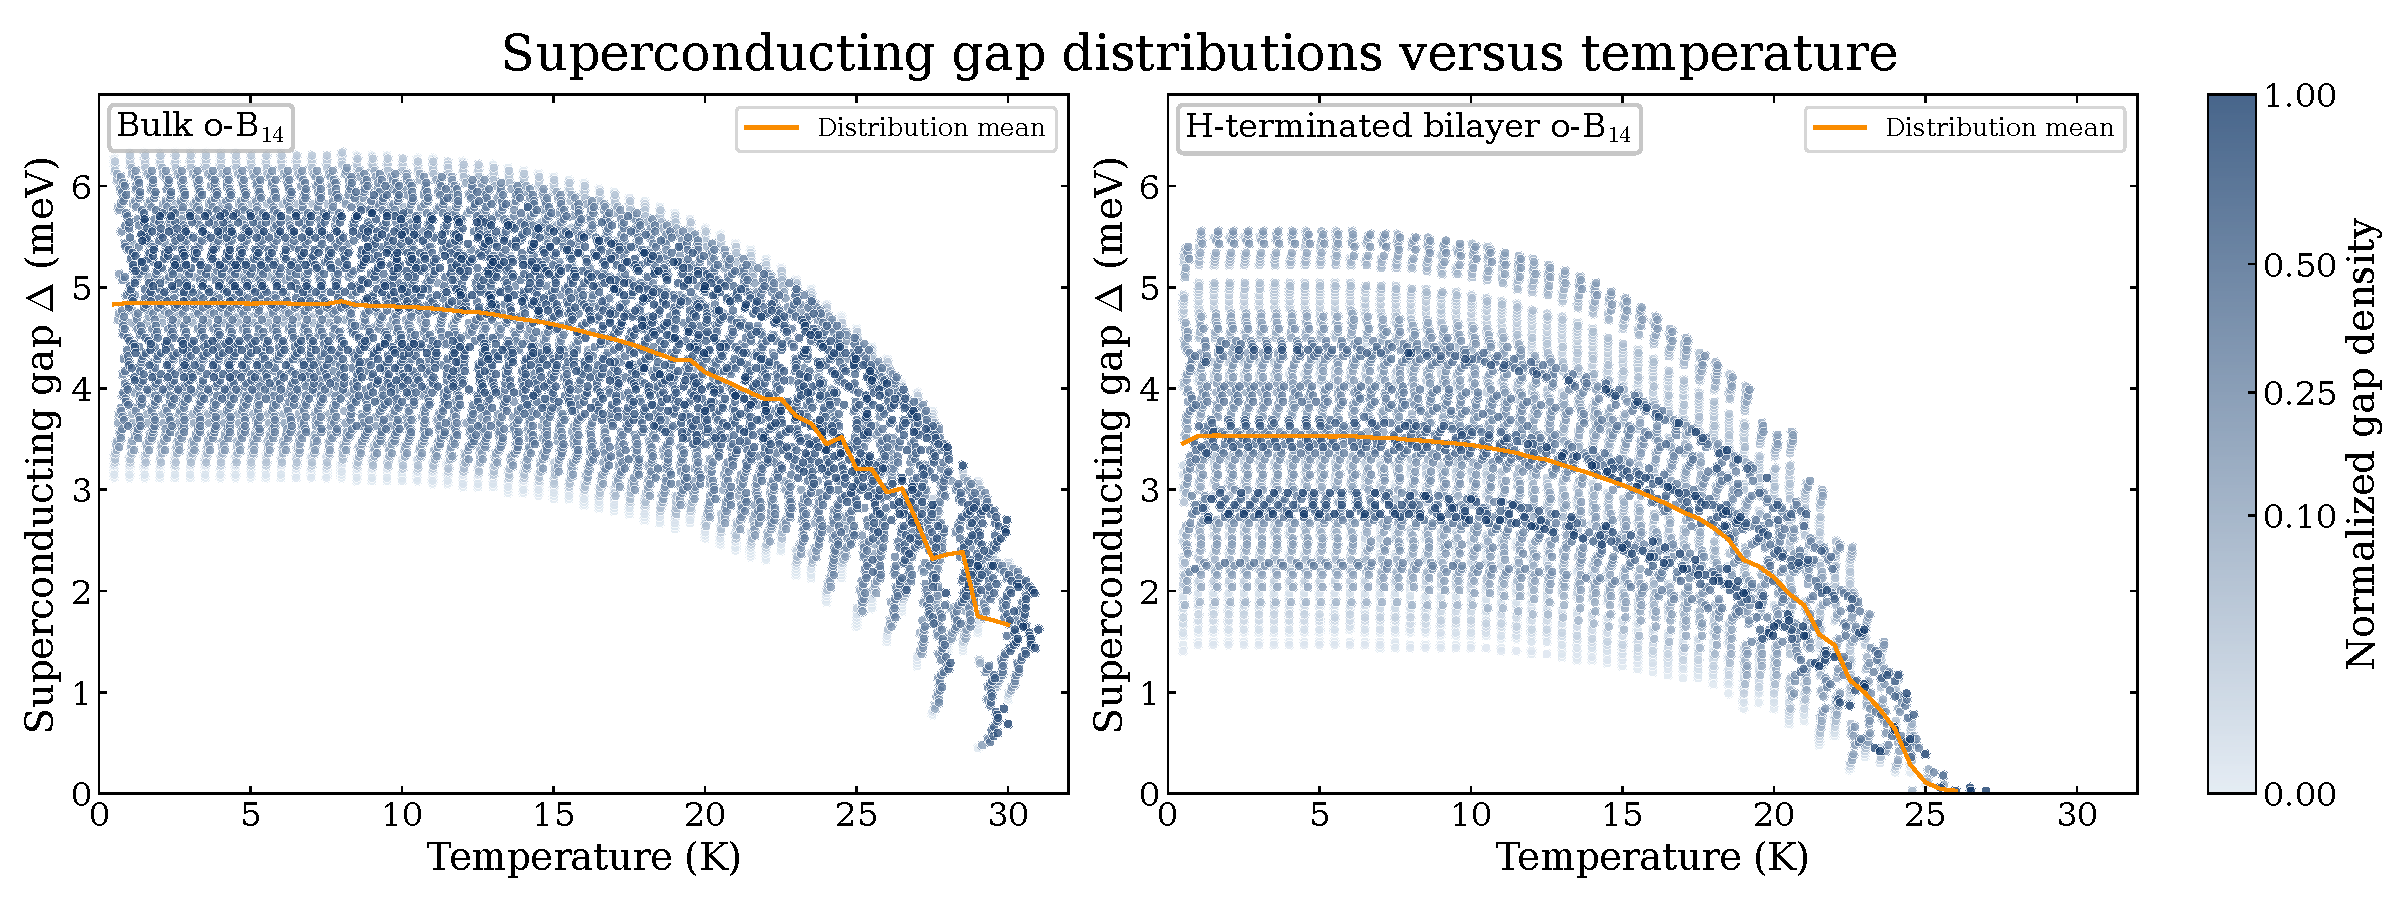
\includegraphics[width=0.80\textwidth]{figures_proj2/fig2.9_alt.pdf}
\caption[Anisotropic superconducting-gap distributions for bulk and hydrogen-terminated bilayer o-\ce{B14}.]{Superconducting gap distributions versus temperature for bulk o-\ce{B14} (left)
and hydrogen-terminated bilayer o-\ce{B14} (right),
obtained from the anisotropic Migdal--Eliashberg treatment with $\mu^*=0.13$.
Colour indicates the normalized distribution at each calculated temperature; the orange line joins its mean values.}
\label{fig:ob14_superconducting_gap}
\end{figure}

The anisotropic Migdal--Eliashberg results in figure~\ref{fig:ob14_superconducting_gap}
show that the gap distribution shifts towards lower energies as the temperature increases.
For bulk o-\ce{B14}, the gap remains finite at the highest calculated temperature of \qty{30}{K}, which places $T_\mathrm{c}$ above \qty{30}{K}.
For the hydrogen-terminated bilayer, the whole gap distribution falls into the lowest gap bin of \qty{0.03}{\milli\electronvolt} at \qty{26}{K}, which places $T_\mathrm{c}$ close to \qty{26}{K}.
Overall, these results suggest that o-\ce{B14} is unlikely to possess conventional superconductivity in the monolayer phase owing to the extremely weak electron-phonon interaction,
whereas the bulk and hydrogen-terminated bilayer are predicted to support phonon-mediated superconductivity.
For the hydrogen-terminated bilayer, the small imaginary phonon frequencies discussed in section~\ref{xene_ob14_phonon_dispersion}
limit the stability assessment.
The Allen--Dynes and anisotropic Migdal--Eliashberg estimates are separate results.

\subsection{Optical properties}
\label{2_optical}

We now use the calculated dielectric tensor to examine the optical response of bulk o-\ce{B14},
monolayer o-\ce{B14}, bilayer o-\ce{B14}, and the hydrogen-terminated bilayer.
In particular, we analyse the real part $\varepsilon_{1}(\omega)$ and imaginary part $\varepsilon_{2}(\omega)$ of the dielectric function.
We then derive the corresponding optical properties from these two components.
All spectra in this section use the non-spin-polarized PBE reference states.
In particular, the metallic monolayer spectrum is distinct from the gapped antiferromagnetic HSE06 state in figure~\ref{fig:monolayer_bilayer_band_structure}.
The bilayer optical calculation likewise uses its PBE semimetallic band structure.

The definitions of the dielectric function and the derived optical quantities are introduced in chapter~\ref{cha:fundamentals_b},
especially section~\ref{sec:from_dielectric_function_to_optical_properties}.
Here, we use $\varepsilon_{1}(\omega)$ to identify the screening response and possible plasmonic regions,
while $\varepsilon_{2}(\omega)$ provides the absorptive part of the optical response.

% Original paper figure 9.
\begin{figure}[!htbp]
\centering
    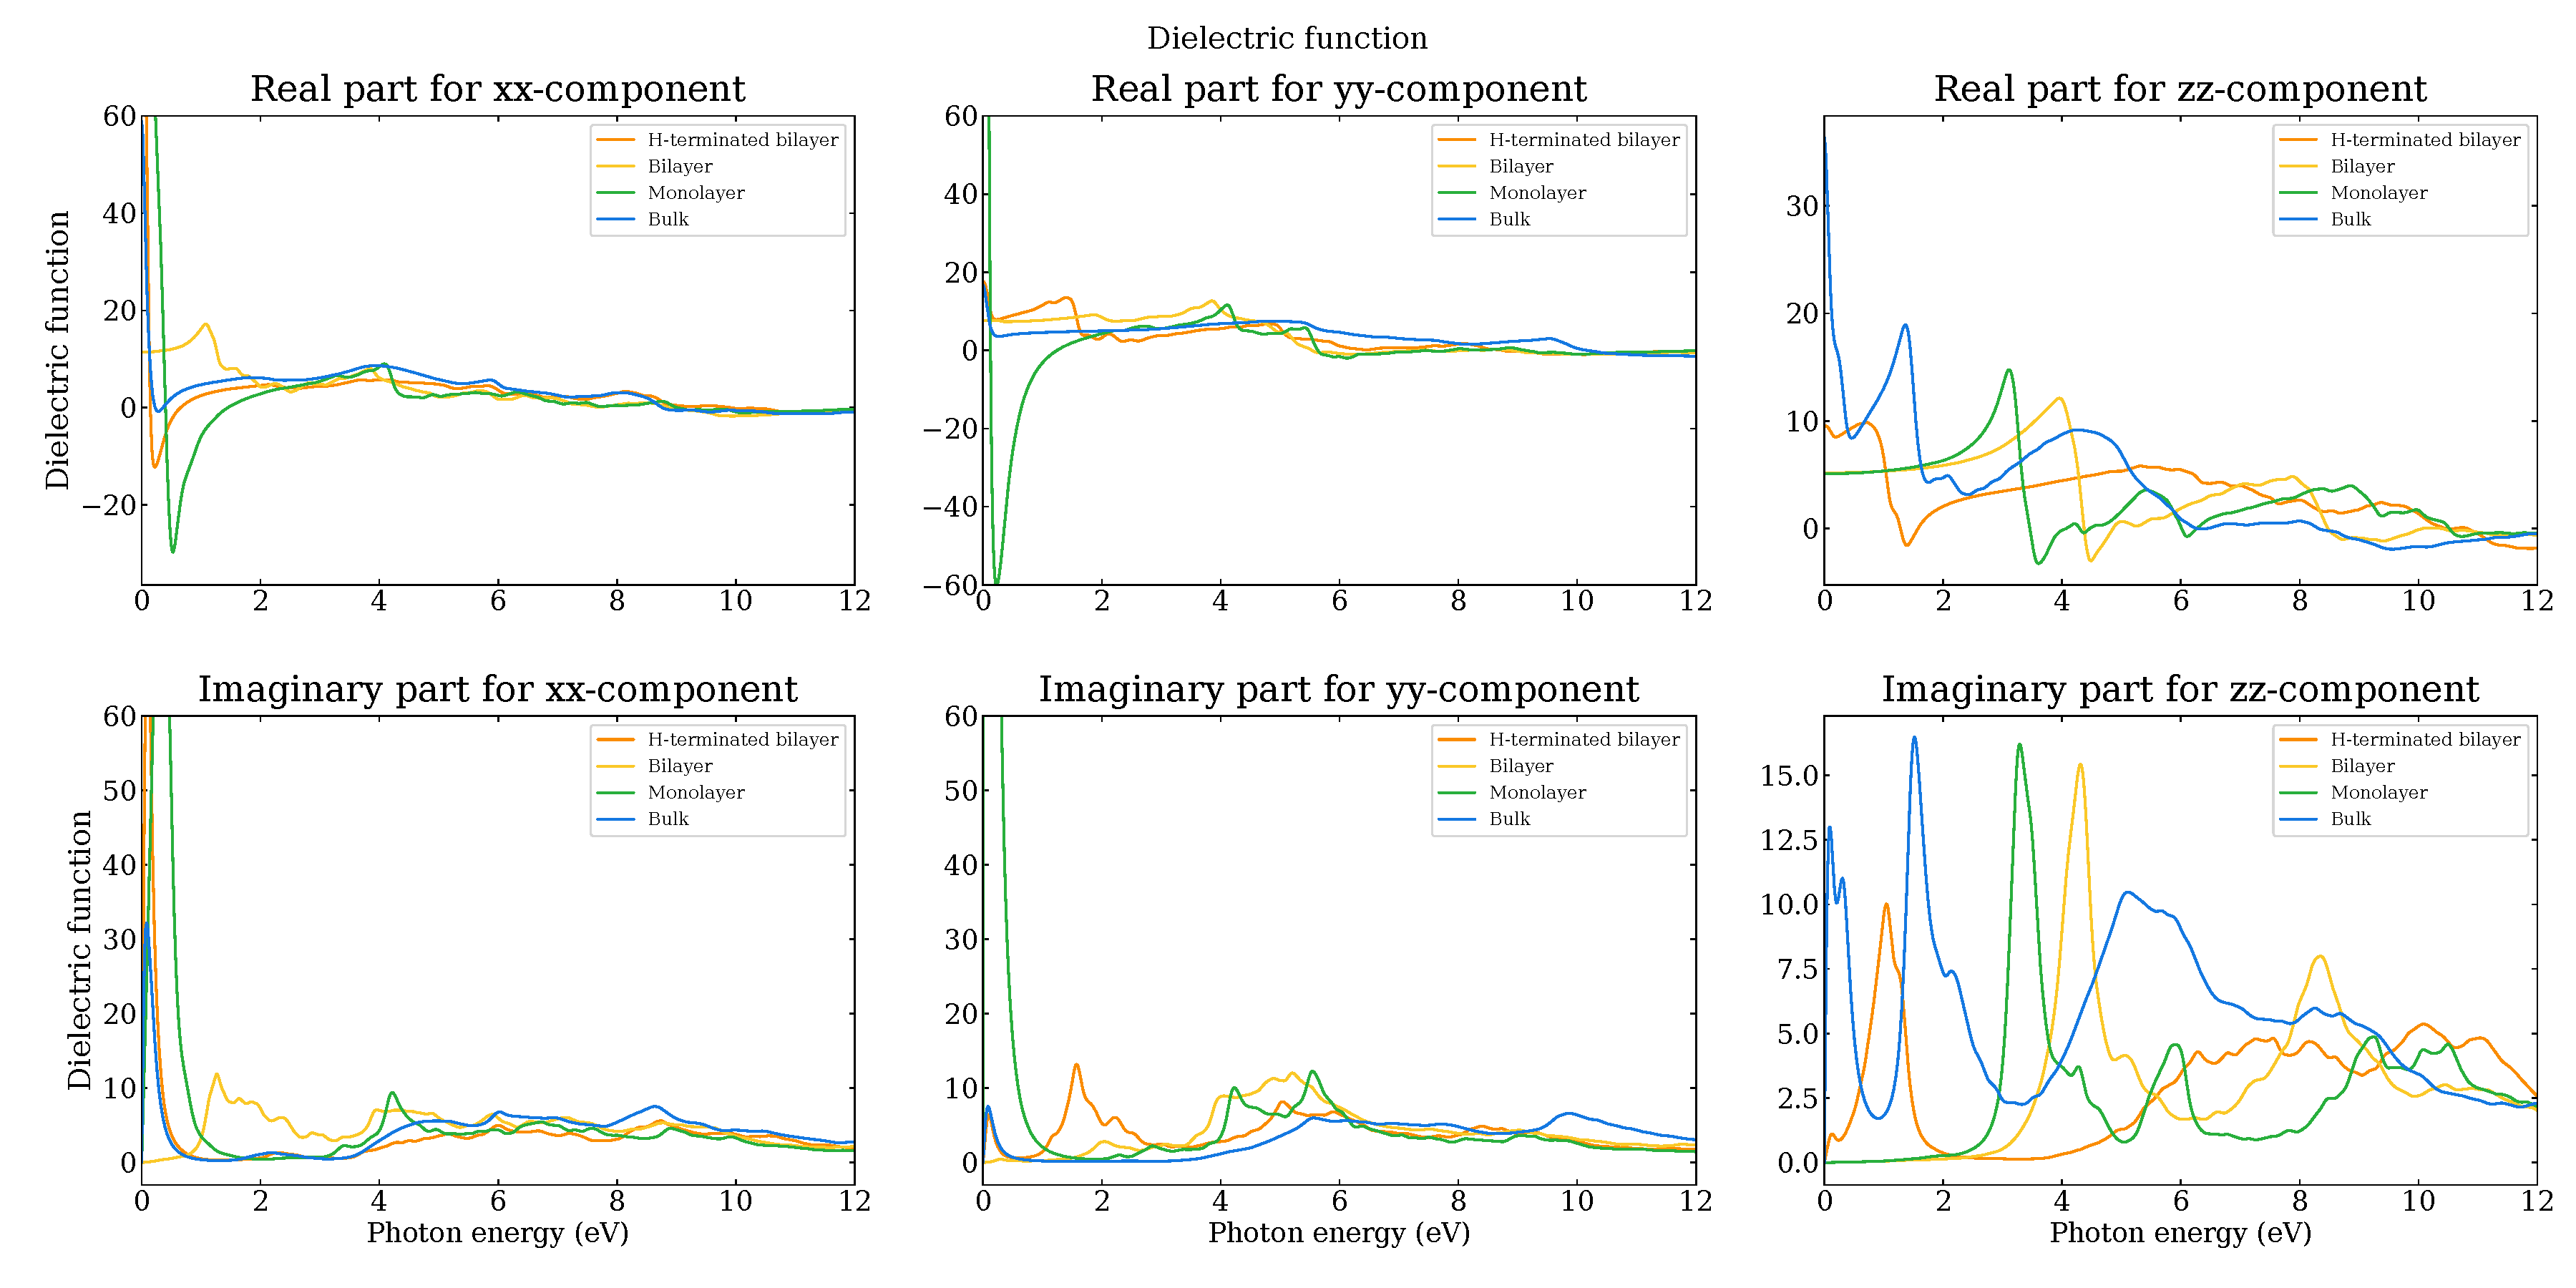
\includegraphics[width=1.00\textwidth]{figures_proj2/fig2.10.pdf}
\caption{Real and imaginary parts of the dielectric function for the bulk and two-dimensional o-\ce{B14} structures for the two in-plane components $xx$ and $yy$, and the out-of-plane component $zz$,
calculated for the non-spin-polarized PBE reference states.}
\label{fig:ob14_dielectric_function}
\end{figure}

Figure~\ref{fig:ob14_dielectric_function} shows the real and imaginary parts of the dielectric function
for all the structures considered, including the two in-plane components $xx$ and $yy$, and the out-of-plane component $zz$.
The difference between the two in-plane components $xx$ and $yy$ and the out-of-plane component $zz$ demonstrates the optical anisotropy of these structures.

For photon energies below around \qty{2.0}{\electronvolt},
the in-plane $xx$ and $yy$ components differ for the bulk and hydrogen-terminated bilayer.
For these systems, $\varepsilon_{1}(\omega)$ for the $xx$ component is negative in part of this region,
whereas the $yy$ component is not.
It can also be seen that, over certain energy ranges,
the monolayer, hydrogen-terminated bilayer, and bulk systems behave as indefinite media,
where the in-plane and out-of-plane components of $\varepsilon_{1}(\omega)$ have opposite signs.
This occurs below \qty{2.0}{\electronvolt} for the monolayer and hydrogen-terminated bilayer,
and between \qty{6.0}{\electronvolt} and \qty{10.0}{\electronvolt} for the bulk.

The corresponding energy-loss spectrum is examined below to distinguish these intervals from resonance peaks.

Peaks in the imaginary part of the dielectric function signal strong absorption due to electronic transitions,
typically interband excitations. Their energy, width, and intensity reflect the band structure and optical response.
Except for the bilayer, the structures show a large low-energy response in these metallic reference calculations.
Since no separately parameterized Drude term is added,
the free-carrier scattering rate and the dc limit lie outside this response.
The bilayer, on the other hand,
has a small $\varepsilon_{2}(\omega)$ at low energy despite its PBE semimetallic band structure,
as a small band overlap can coexist with weak optical transitions.
The dielectric tensor characterizes how the polarization of the material changes in response to an applied electric field.
For an incident photon,
the tensor components represent the material response to the electric-field component of the photon along different directions.
For all systems studied here,
the off-diagonal components of the dielectric tensor are zero.

\begin{figure}[!htbp]
\centering
    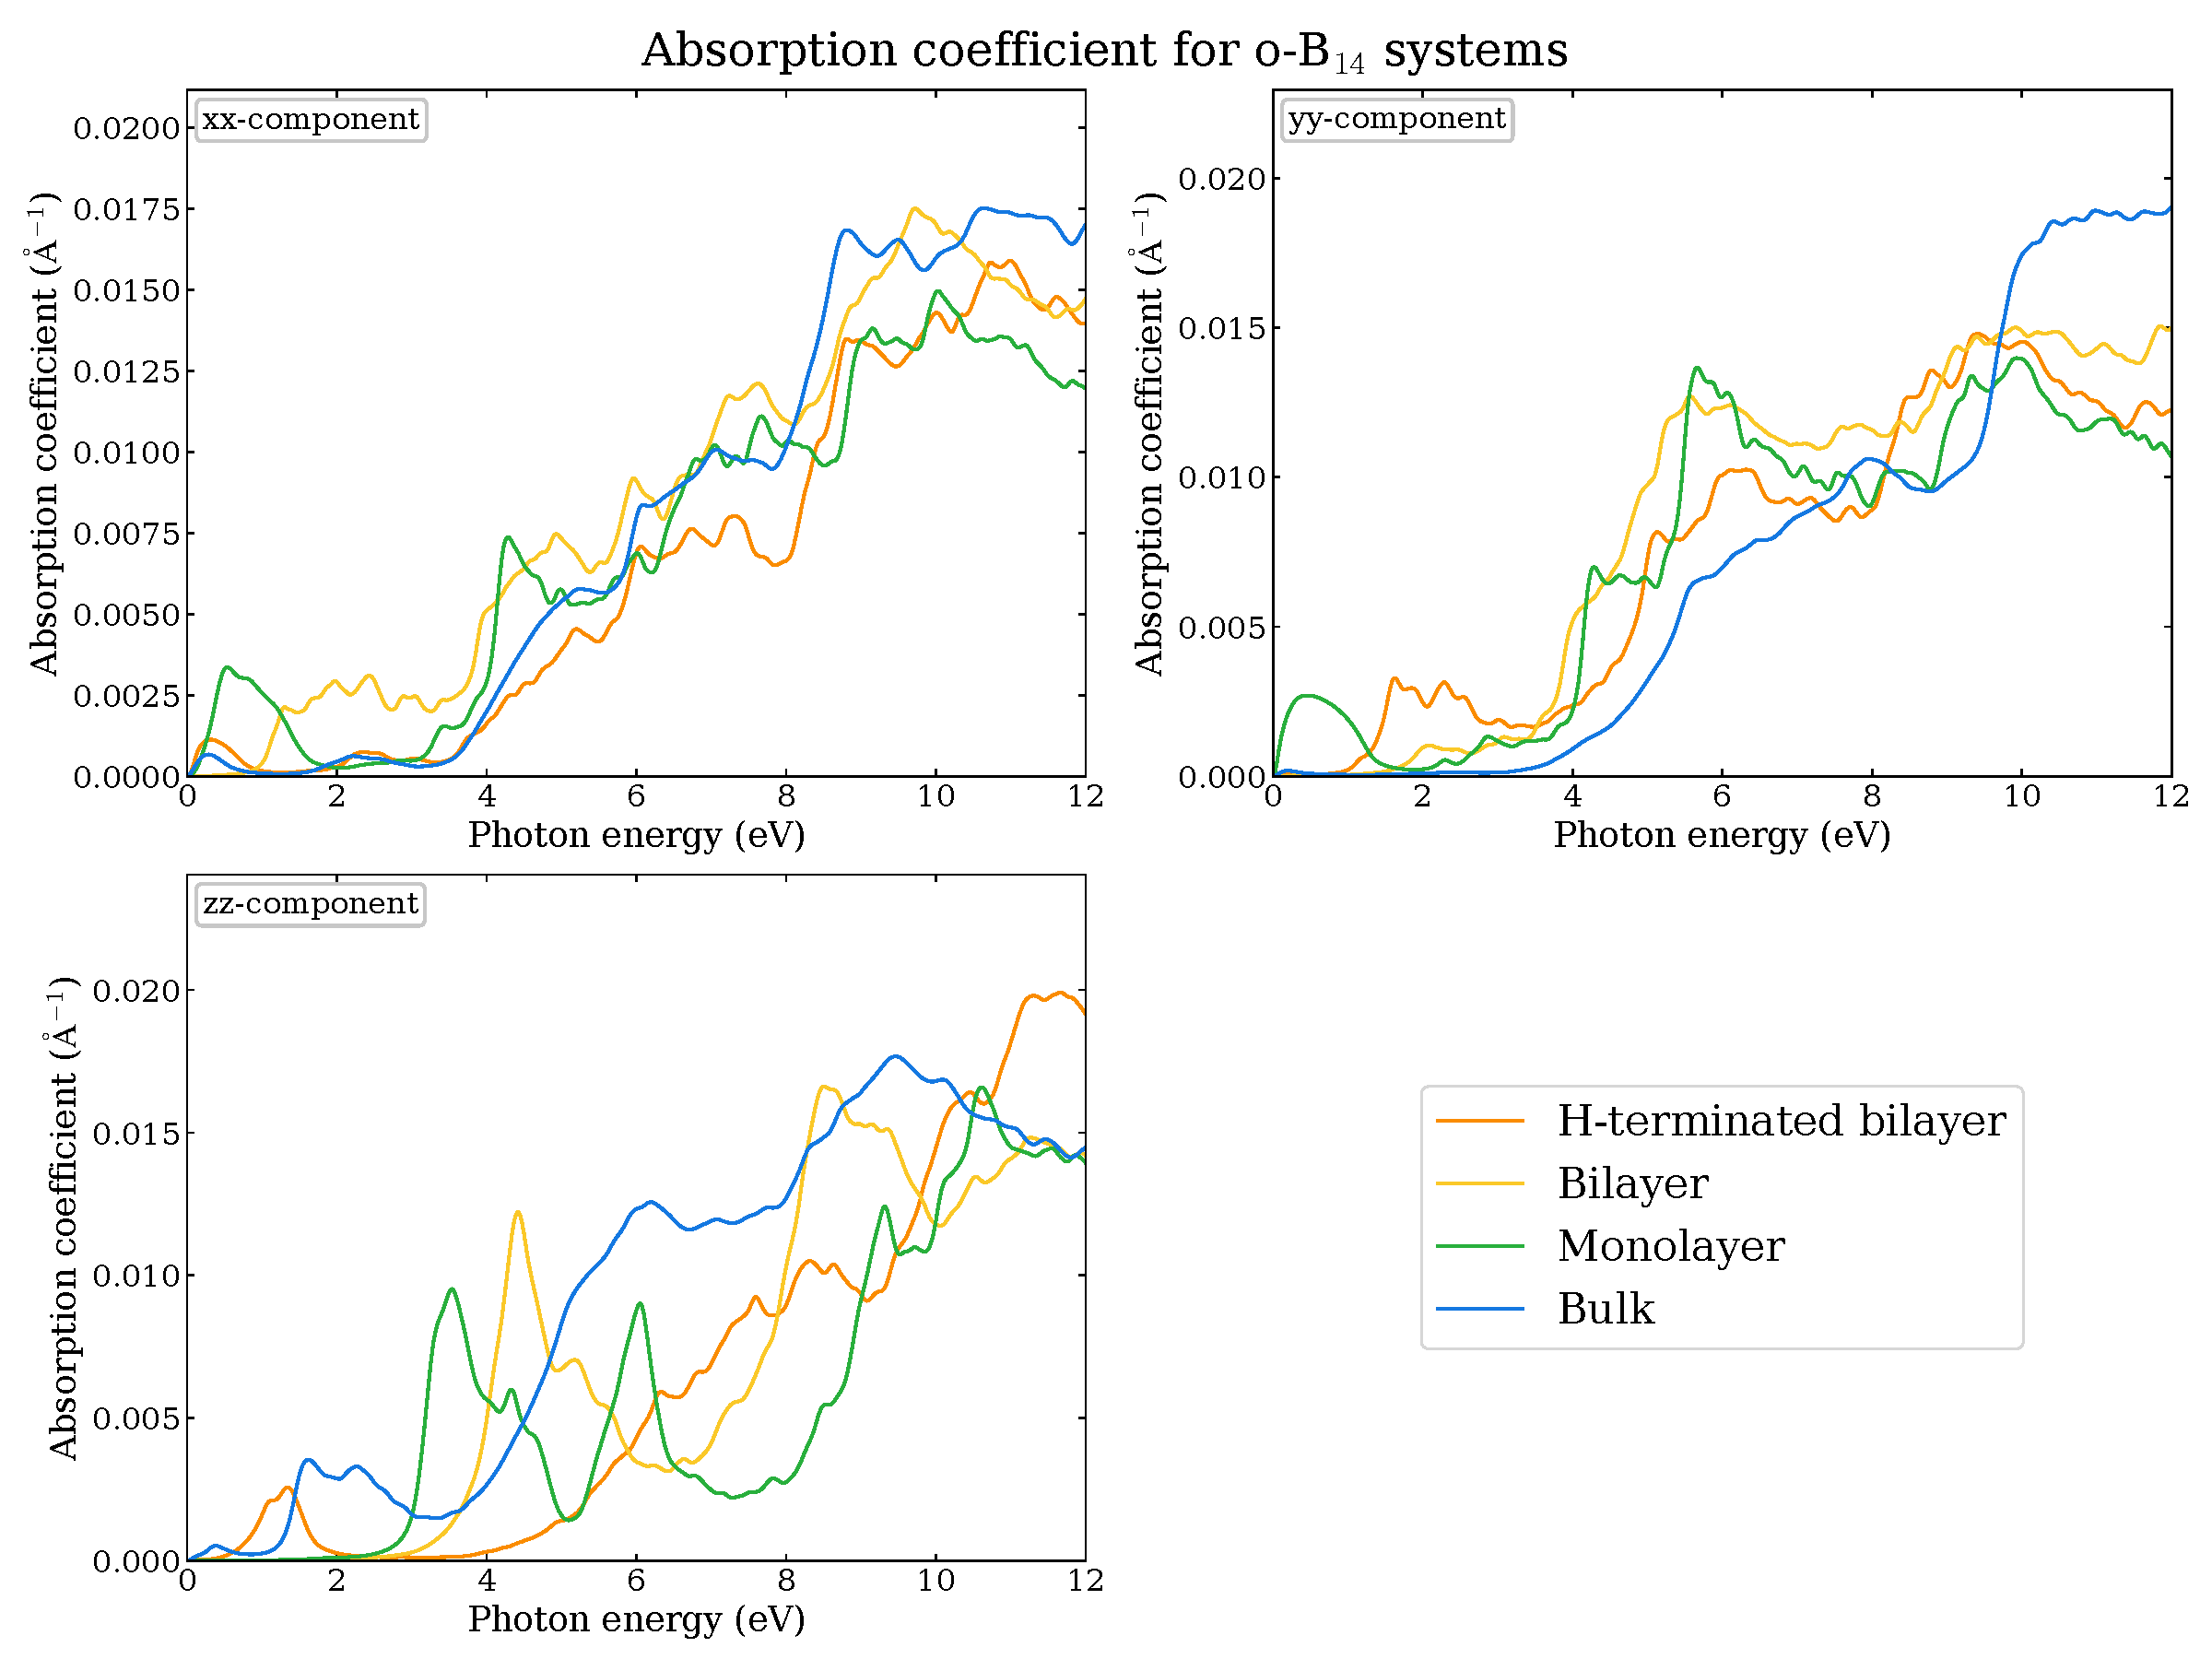
\includegraphics[width=0.80\textwidth]{figures_proj2/fig2.11a.pdf}
    \par\nointerlineskip
    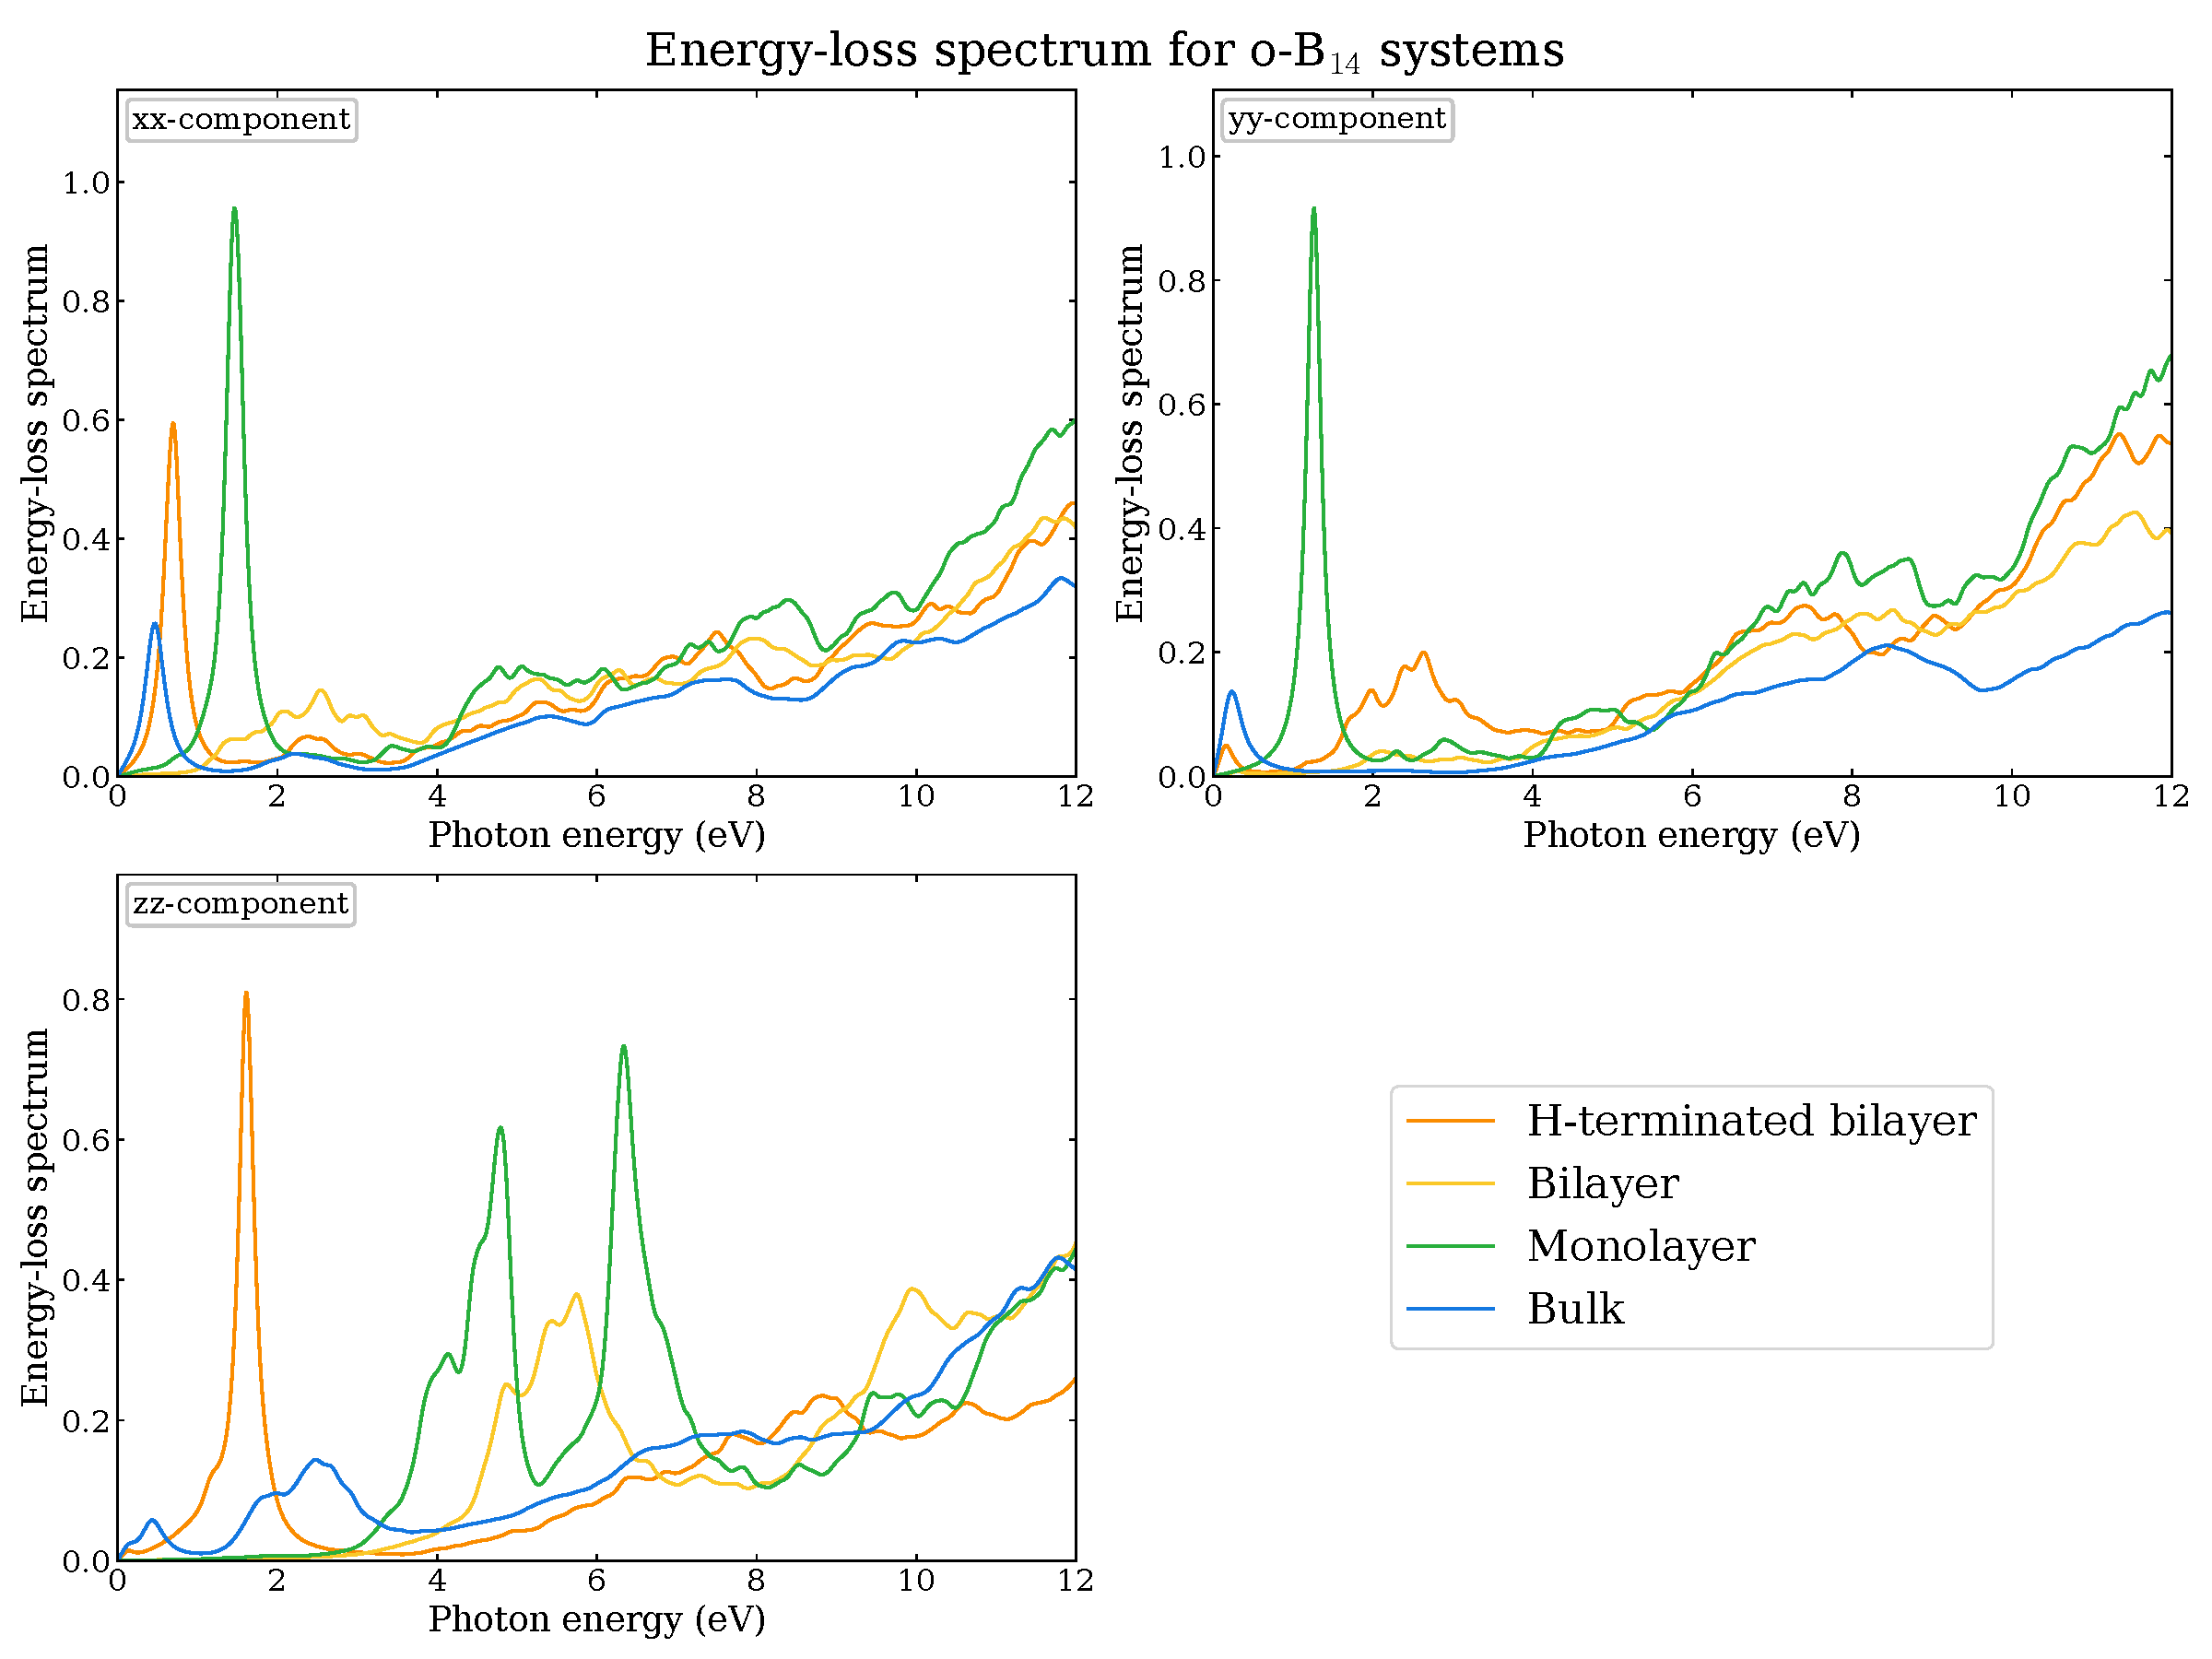
\includegraphics[width=0.80\textwidth]{figures_proj2/fig2.11b.pdf}
\caption{Absorption coefficient and energy-loss spectrum for the bulk and two-dimensional o-\ce{B14} structures
for the in-plane $xx$ and $yy$ directions,
and the out-of-plane $zz$ direction.
The absorption coefficient is given in \si{\per\angstrom}; the energy-loss function is dimensionless.}
\label{fig:ob14_absorption_loss}
\end{figure}

We then calculate the absorption coefficient, energy-loss spectrum, reflectivity, refractive index,
and extinction coefficient from the dielectric function.
Figure~\ref{fig:ob14_absorption_loss} shows the absorption coefficient and energy-loss spectrum for the various structures.
The absorption coefficient is obtained from both parts of the dielectric function through
$\alpha(\omega)=2\omega k(\omega)/c$,
as given in equation~\eqref{absorption_coefficient_from_extinction_coefficient}.
Here, $\omega$ is the angular frequency, with photon energy $E=\hbar\omega$.
The absorption onset can differ from the first maximum of $\varepsilon_{2}(\omega)$.
The bulk, monolayer, and hydrogen-terminated bilayer show appreciable low-energy absorption in the present reference calculations.

In the visible region of the spectrum, from \qty{1.7}{\electronvolt} to \qty{3.3}{\electronvolt},
the bilayer, hydrogen-terminated bilayer, and bulk systems have the largest absorption coefficients for the $xx$,
$yy$, and $zz$ components, respectively.
The monolayer, on the other hand, exhibits strong absorption in the near-infrared and ultraviolet regions.
Related first-principles studies have also considered the optical response of bulk and bilayer silicon~\cite{saunders2024structural}.
A quantitative comparison requires consistent absorption units and, for the layers, a consistent effective-thickness convention.

The energy-loss spectrum in figure~\ref{fig:ob14_absorption_loss} exhibits several sharp peaks.
Beyond a negative $\varepsilon_1$, an energy-loss maximum close to a zero crossing of $\varepsilon_1$, with sufficiently small $\varepsilon_2$,
provides the optical-limit signature of a plasmon resonance.
A wave-vector-dependent response would give the dispersion of a propagating two-dimensional plasmon.
For the $xx$ component, the bulk, monolayer, and hydrogen-terminated bilayer show energy-loss features below approximately \qty{1.5}{\electronvolt}.
The monolayer also shows a distinct feature in the $yy$ direction.
The finite $\varepsilon_2(\omega)$ near the corresponding zero crossings indicates damping, especially for the bulk.
In the out-of-plane direction, the hydrogen-terminated bilayer has a strong peak near \qty{1.6}{\electronvolt}.
The monolayer has features in the \qtyrange{4}{5}{\electronvolt} region and near \qty{6}{\electronvolt},
while the bilayer has features around \qtyrange{5}{6}{\electronvolt}.
The negative-$\varepsilon_1$ intervals and the energy-loss maxima can have different boundaries.

\begin{figure}[!htbp]
\centering
    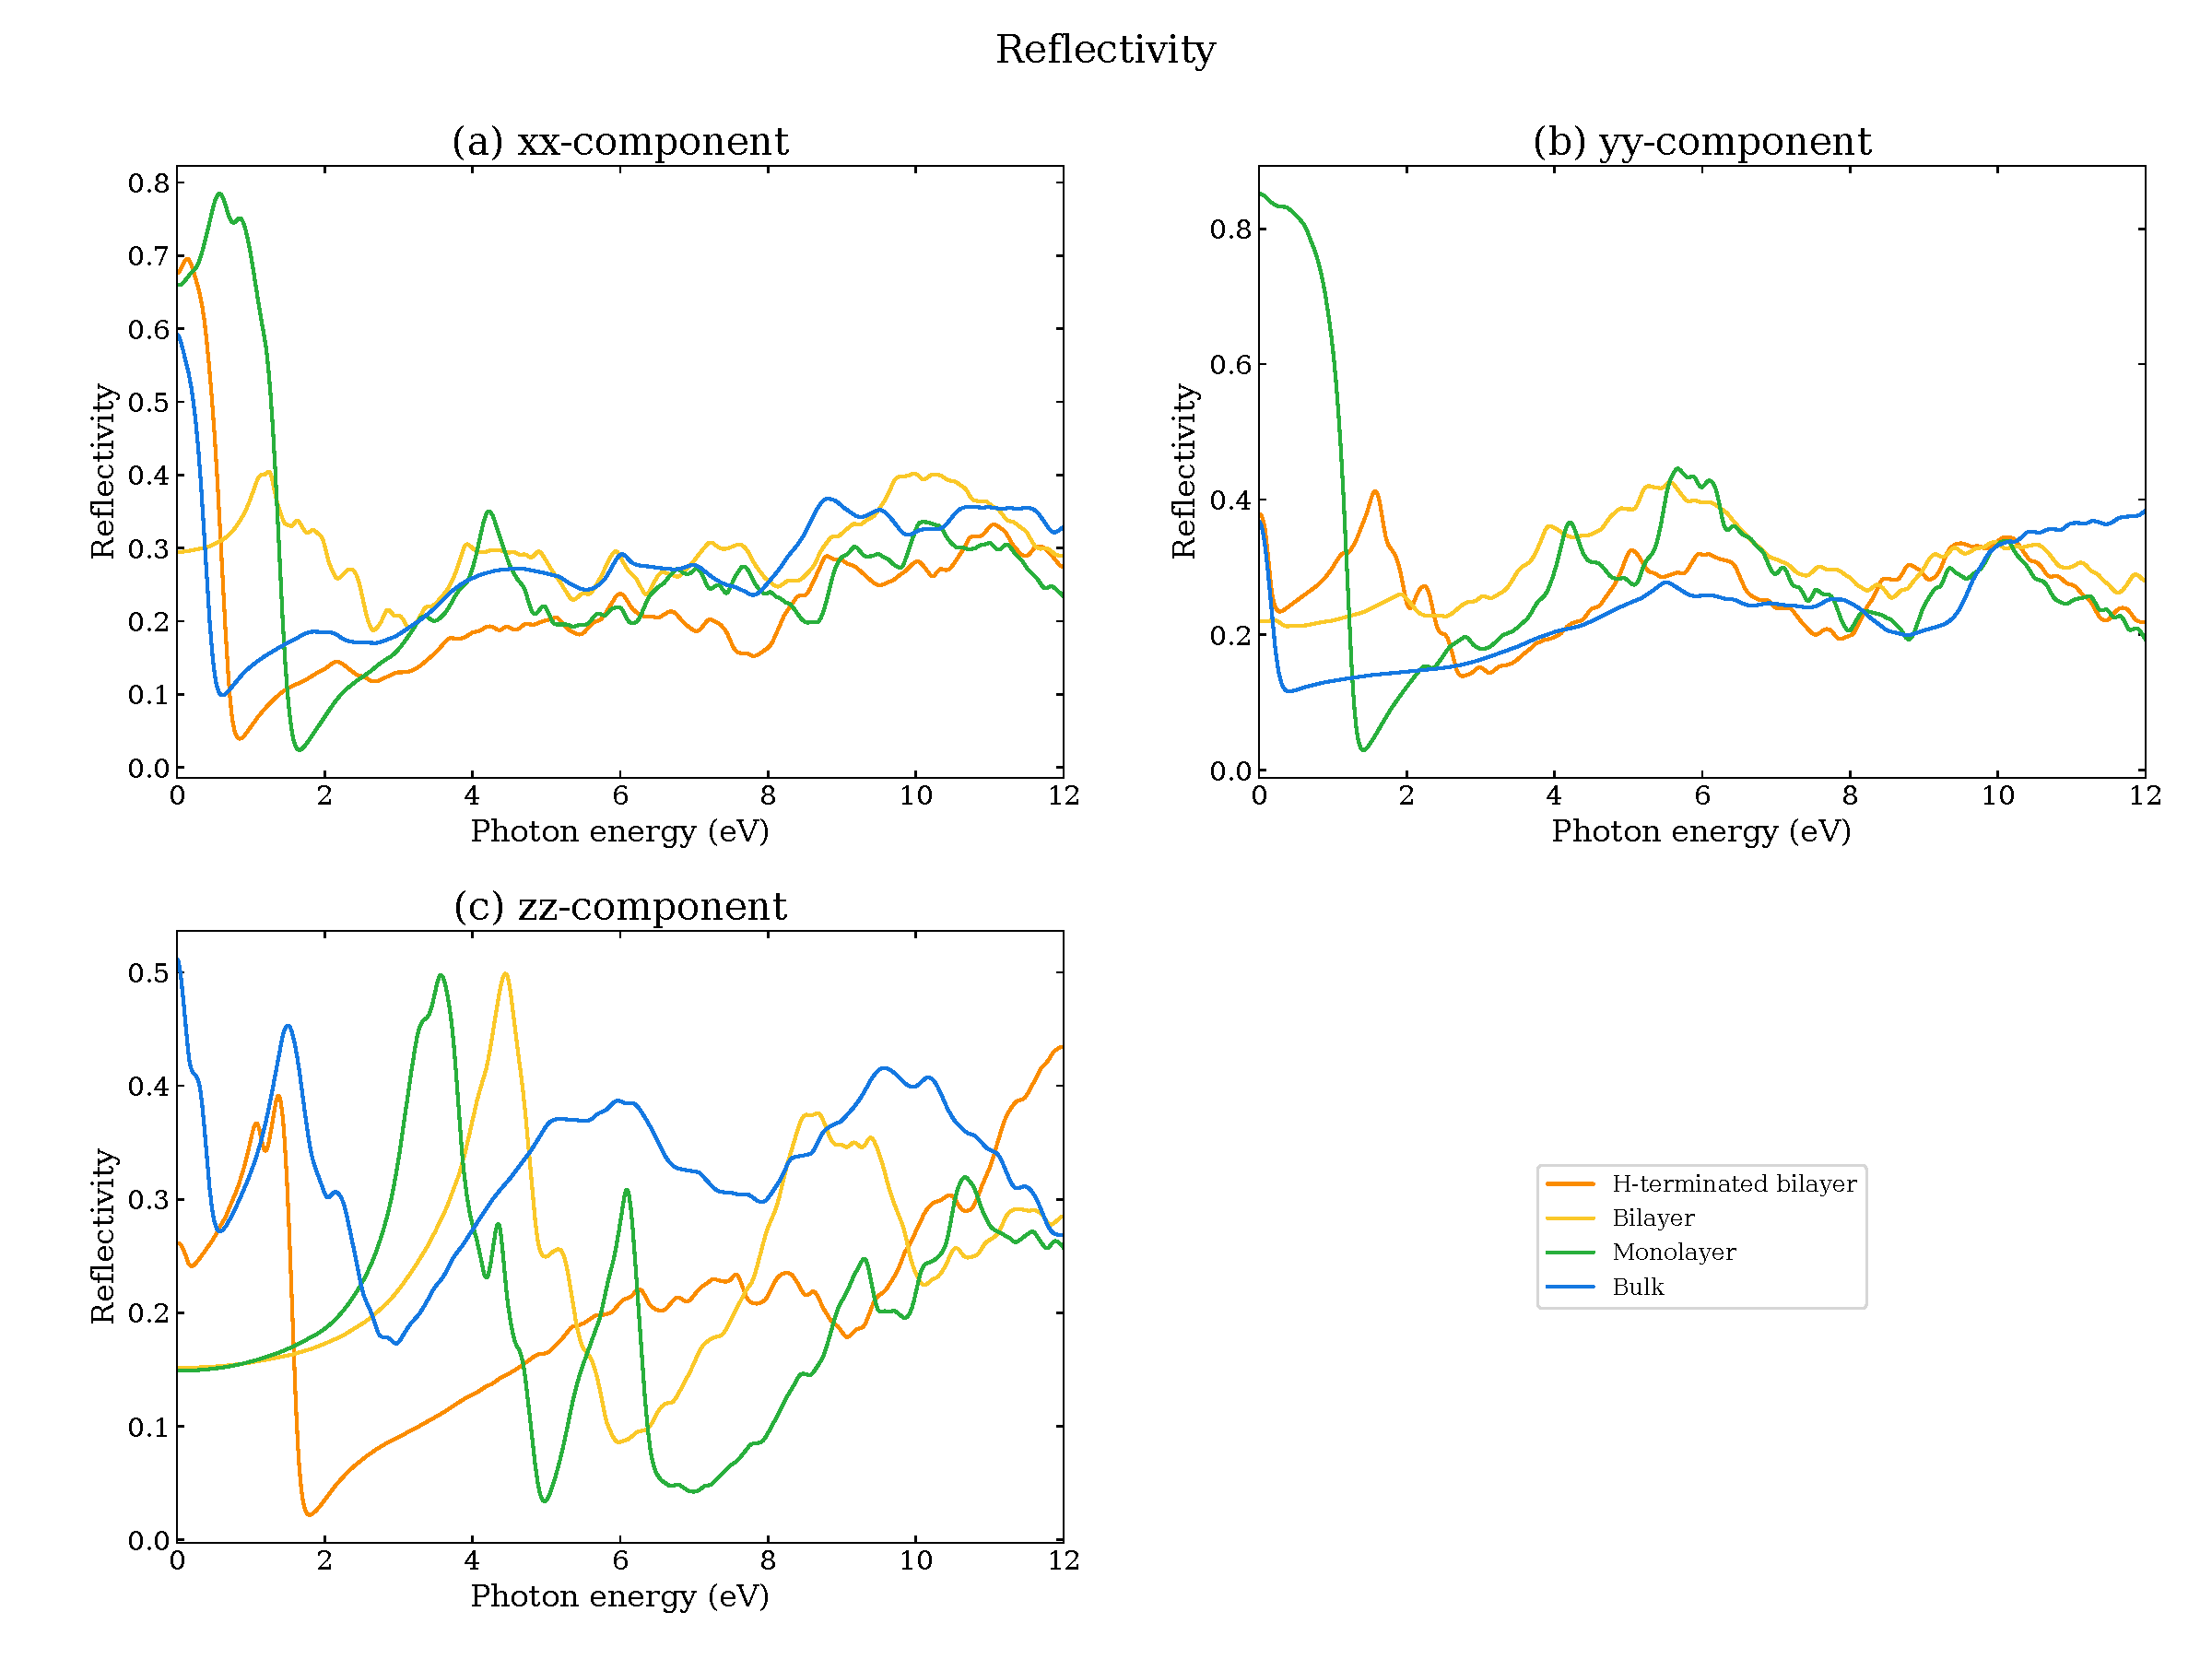
\includegraphics[width=0.80\textwidth]{figures_proj2/fig2.12a.pdf}
    \par\nointerlineskip
    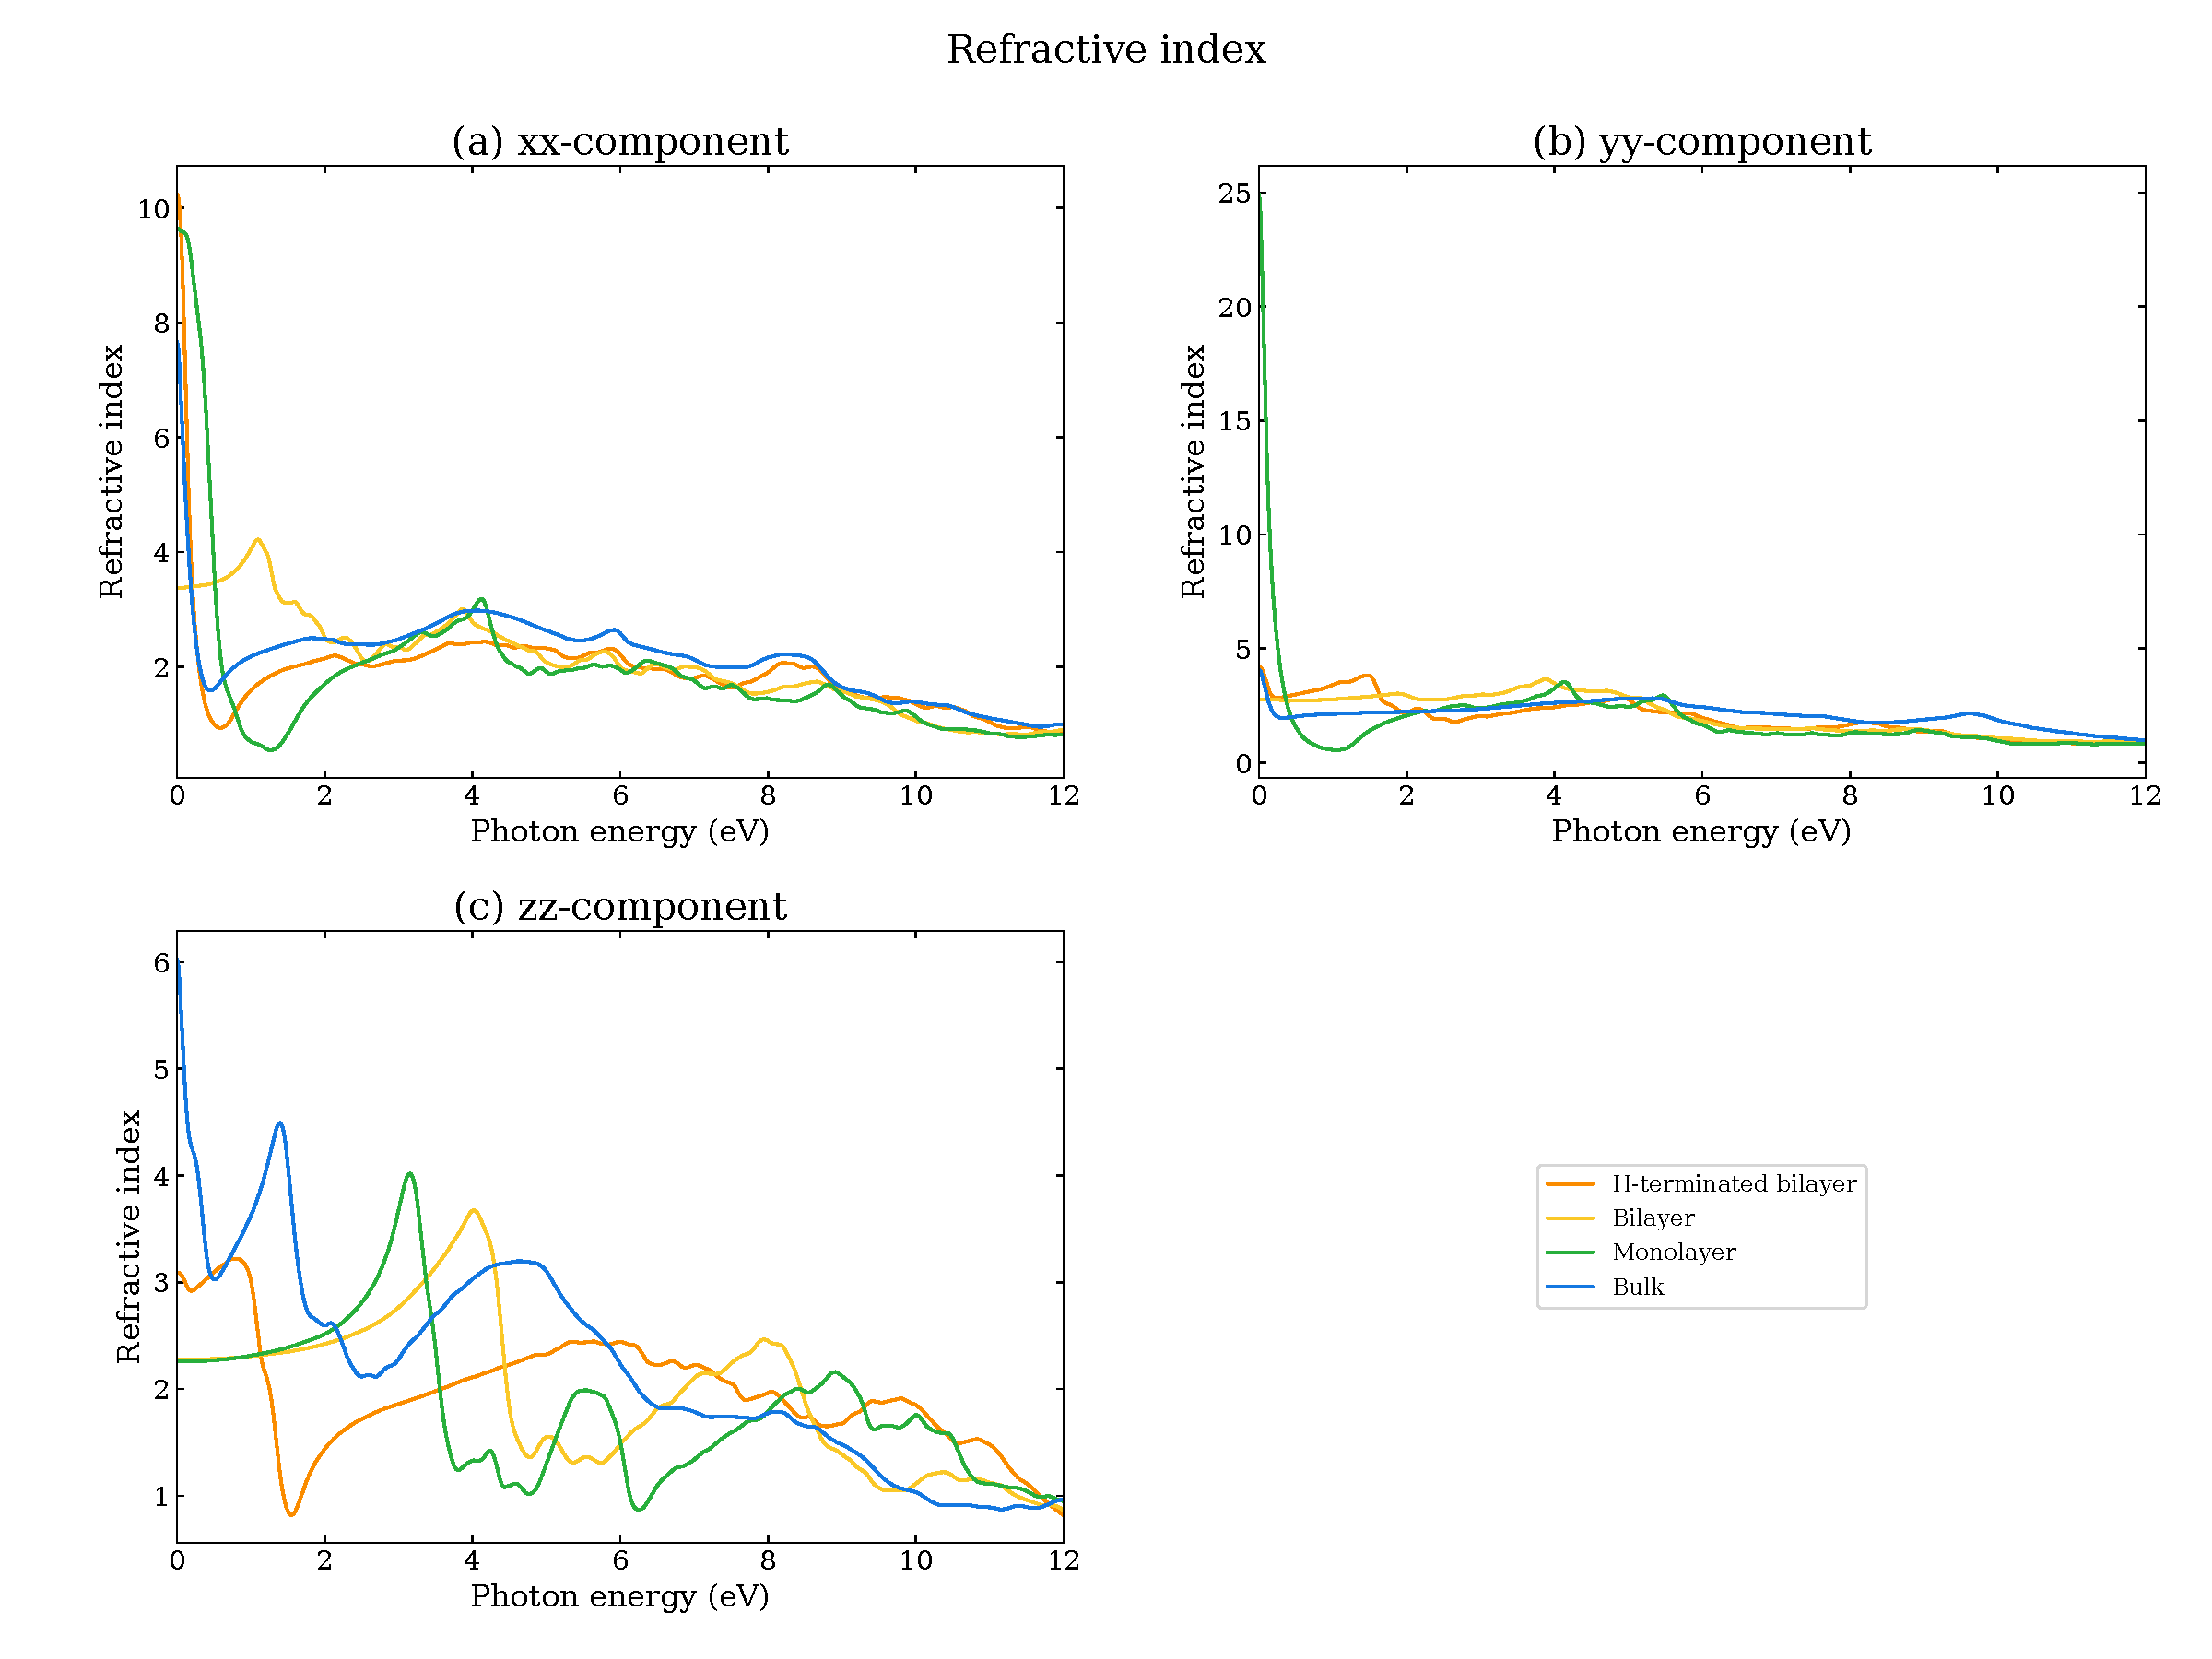
\includegraphics[width=0.80\textwidth]{figures_proj2/fig2.12b.pdf}
\caption{Reflectivity and refractive index as functions of photon energy for the bulk and two-dimensional o-\ce{B14} structures
for the in-plane $xx$ and $yy$ directions,
and the out-of-plane $zz$ direction.}
\label{fig:ob14_reflectivity_refractive_index}
\end{figure}

Figure~\ref{fig:ob14_reflectivity_refractive_index} shows the reflectivity and refractive index.
The reflectivity features directly reflect the electronic structure,
where the drops in reflectivity correlate with the edges of the plasmonic features discussed above.
The trends in refractive index are similar to those of $\varepsilon_{1}(\omega)$,
which indicates that the real part of the dielectric function plays the leading role in the refractive-index response.

For visible light, most transparent materials have refractive indices between one and two.
Near a plasmon resonance in two-dimensional materials,
the refractive index can drop below one due to the strong interaction between light and plasmonic oscillations.
Metals can have a high refractive index at low photon energies due to strong absorption.
As the photon energy increases, the refractive index decreases to values between one and two,
particularly near or beyond interband transitions and the plasma edge.

For in-plane polarization, the refractive index of the monolayer is close to,
and smaller than, one in the energy range from around \qty{0.5}{\electronvolt} to \qty{1.5}{\electronvolt}.
For out-of-plane polarization, this occurs at around \qty{1.5}{\electronvolt} for the hydrogen-terminated bilayer,
\qty{3.6}{\electronvolt} and \qty{6.0}{\electronvolt} for the monolayer,
and around \qty{4.8}{\electronvolt} for the bilayer.
These energy ranges are close to the plasmonic features discussed above.

The extinction coefficient shown in figure~\ref{S2.18} provides information on how strongly a material absorbs light at different photon energies.
It is noticeable that the extinction coefficient exhibits sharp dips or peaks near the plasmon resonances discussed above.
Near a plasmon resonance,
the dielectric function changes rapidly in both its real and imaginary parts,
which affects the extinction coefficient and produces sharp features,
including dips or peaks, near resonances.
These features follow from the same dielectric function, so they repeat the evidence of the energy-loss spectrum for the plasmon assignment.

Specifically, these dips or peaks occur around \qty{0.5}{\electronvolt} and \qty{1.3}{\electronvolt} for the $xx$ component,
\qty{1.0}{\electronvolt} and \qty{6.0}{\electronvolt} for the $yy$ component,
and \qty{3.5}{\electronvolt} and \qty{6.0}{\electronvolt} for the $zz$ component of the monolayer.
For the bilayer, they occur around \qty{2.0}{\electronvolt} for the $yy$ component,
and \qty{4.5}{\electronvolt} and \qty{9.0}{\electronvolt} for the $zz$ component.
For the hydrogen-terminated bilayer, they occur around \qty{0.5}{\electronvolt} for the $xx$ component,
\qty{2.0}{\electronvolt} and \qty{6.0}{\electronvolt} for the $yy$ component,
and \qty{1.5}{\electronvolt} for the $zz$ component.
For the bulk, they occur around \qty{0.5}{\electronvolt} and \qty{8.8}{\electronvolt} for the $xx$ component,
\qty{0.2}{\electronvolt} and \qty{10.0}{\electronvolt} for the $yy$ component,
and \qty{0.5}{\electronvolt}, \qty{2.0}{\electronvolt},
and in the range from \qty{6.3}{\electronvolt} to \qty{8.3}{\electronvolt} for the $zz$ component.

Overall, the plasmonic and optical properties of the o-\ce{B14} structures display anisotropic effects,
which may offer opportunities for optoelectronic,
plasmonic, and quantum devices.

\section{Conclusions}
\label{2_conclusions}

In the present chapter, we investigated the electronic, optical,
and superconducting properties of novel o-\ce{B14}-based structures using density functional theory.
Namely, we considered the three-dimensional bulk as well as the two-dimensional monolayer,
bilayer, and hydrogen-terminated bilayer.
The cohesive energies of the monolayer and bilayer are less negative than that of the bulk by \qty{0.35}{\electronvolt} and \qty{0.12}{\electronvolt} per atom, respectively.
These comparisons concern the calculated cohesive energies.
The two-dimensional allotropes of o-\ce{B14} reveal complex properties including semiconductivity in the bilayer with a band gap of \qty{0.67}{\electronvolt},
magnetism in the monolayer, and predicted phonon-mediated superconductivity in the hydrogen-terminated bilayer.
The calculated optical properties show absorption in the visible region of the spectrum for the bilayer in the in-plane $xx$ component,
the hydrogen-terminated bilayer in the in-plane $yy$ component,
and the bulk in the out-of-plane $zz$ component.

The metallic reference systems show in-plane energy-loss features below around \qty{1.5}{\electronvolt},
while all systems show out-of-plane energy-loss features.
Their plasmonic interpretation depends on the damping and the effective-medium treatment of the layers.
Interestingly, the monolayer, hydrogen-terminated bilayer, and bulk systems behave as indefinite media,
for which the real part of the dielectric function in the in-plane and out-of-plane directions has opposite signs.
This occurs in the region below \qty{2.0}{\electronvolt} for the monolayer and hydrogen-terminated bilayer,
and between \qty{6.0}{\electronvolt} and \qty{10.0}{\electronvolt} for the bulk.
Altogether, these complex optical, electronic,
and superconducting properties emphasize the rich physics of boron materials,
which could hold potential for future high technologies.

\clearpage
\section{Data availability statement}

The archived calculation and plotting data for this chapter are available from the \texttt{GitHub} repository:
\href{https://github.com/Photonico/o-B14_20241024}{\texttt{Photonico/o-B14\_20241024}}.

\section{Supplementary information}
\label{2_supplementary}

Convergence tests are shown for the total energy, the plane-wave energy cutoff,
and the k-point set of bulk o-\ce{B14} in figure~\ref{S2.1}.
The lattice-constant determination is shown in the right panel of figure~\ref{S2.1},
and the cohesive-energy convergence is shown in figure~\ref{S2.2}.
The total energy as a function of the supercell length normal to the monolayer is given in figure~\ref{S2.3}.
Convergence tests for the calculation of the dielectric function are also shown for the k-point set in figure~\ref{S2.4}
and for the total number of bands, including unoccupied states, in figure~\ref{S2.5}.
The definition of $d_{\mathrm{2D}}$ used in the dielectric-function renormalization is displayed in figure~\ref{S2.6}.
The renormalization procedure is given in section~\ref{2_methods},
and the general optical-property definitions are introduced in chapter~\ref{cha:fundamentals_b}.
Figure~\ref{S2.7} shows the hollow-bridge site that was also considered for hydrogen adsorption on the monolayer and bilayer structures.

The calculated phonon-dispersion curves for the two-dimensional systems,
as obtained using $(2 \times 2)$ and $(3 \times 3)$ supercells, are shown in figures~\ref{S2.8} and~\ref{S2.9}.
The results obtained using both supercells show qualitatively the same behaviour.
The hydrogen-terminated monolayer is dynamically unstable due to imaginary frequencies across a wide range of the Brillouin zone.

Results of \textit{ab initio} molecular dynamics (AIMD) calculations for the hydrogen-terminated bilayer are shown in figure~\ref{S2.10} for a temperature of \qty{400}{K}, with the bonding framework retained over the simulated \qty{5.5}{ps}.

Comparison of the spin-polarized FM band structures for the monolayer,
as calculated using the GGA-PBE and HSE06 functionals, is shown in figure~\ref{S2.11}.
The PBE total density of states (DoS) of the different structures is shown in figure~\ref{S2.12}.
A comparison of the non-spin-polarized band structure of the monolayer,
as calculated using the r$^{2}$SCAN, HSE06, and GGA-PBE functionals, is shown in figure~\ref{S2.13}.
In figure~\ref{S2.14}, the non-spin-polarized band structure of the monolayer is shown as calculated in a $(2\times1)$ supercell without symmetry,
which tests the effect of possible Jahn--Teller distortions.
For the monolayer structure, the fixed-spin energy profile is shown in figure~\ref{S2.15}, where a clear energy minimum appears near a fixed spin moment of $2.0~\mu_{\mathrm{B}}$.
The spin-resolved total DoS for the FM and AFM monolayers is shown in figure~\ref{S2.16}.
Figure~\ref{S2.17} displays the spin density and the state distribution for the highest occupied and lowest unoccupied states of the FM monolayer midway along the $\mathrm{T}$--$\mathrm{Y}$ direction.
Finally, the frequency-dependent extinction coefficient for all structures considered is displayed in figure~\ref{S2.18}.

\subsubsection*{Optical-property definitions}

We obtain the optical observables used in this chapter from the frequency-dependent dielectric function.
Chapter~\ref{cha:fundamentals_b} introduced the general route from the dielectric function to optical properties in section~\ref{sec:from_dielectric_function_to_optical_properties}.
Specifically,
we defined the absorption coefficient $\alpha_{\lambda}(\omega)$ in equation~\eqref{absorption_coefficient_from_dielectric_function},
the refractive index $n_{\lambda}(\omega)$ in equation~\eqref{refractive_index_from_dielectric_response},
the extinction coefficient $k_{\lambda}(\omega)$ in equation~\eqref{extinction_coefficient_from_dielectric_response},
the reflectivity $R_{\lambda}(\omega)$ in equation~\eqref{reflectivity_from_refractive_index_and_extinction_coefficient},
and the energy-loss spectrum $L_{\lambda}(\omega)$ in equation~\eqref{energy_loss_spectrum_from_dielectric_function}.
Therefore, we do not repeat these formula definitions here.

\subsubsection*{Renormalization of the dielectric function to account for the vacuum region}

The effective thickness of the 2D systems, $d_{\mathrm{2D}}$,
is required for the dielectric-function renormalization introduced in section~\ref{2_methods}.
We define it from the difference in the $z$ coordinate of the top and bottom atoms in the system, $dz$,
together with one additional van der Waals radius on each side of the slab.
Thus, $d_{\mathrm{2D}}=dz+2d_{\mathrm{vdW}}$.
For the bare monolayer and bilayer,
the top and bottom atoms are the pyramidal apical boron atoms.
For the hydrogen-terminated bilayer,
the top and bottom atoms are the H atoms.
Here, we use $d_{\mathrm{vdW}}=\qty{1.91}{\angstrom}$ for boron and $d_{\mathrm{vdW}}=\qty{1.2}{\angstrom}$ for hydrogen.
A schematic illustration of the total thickness, $D_{\mathrm{total}}\coloneqq d_{\mathrm{2D}}$,
is shown in figure~\ref{S2.6}.

\begin{figure}[!htbp]
\centering
    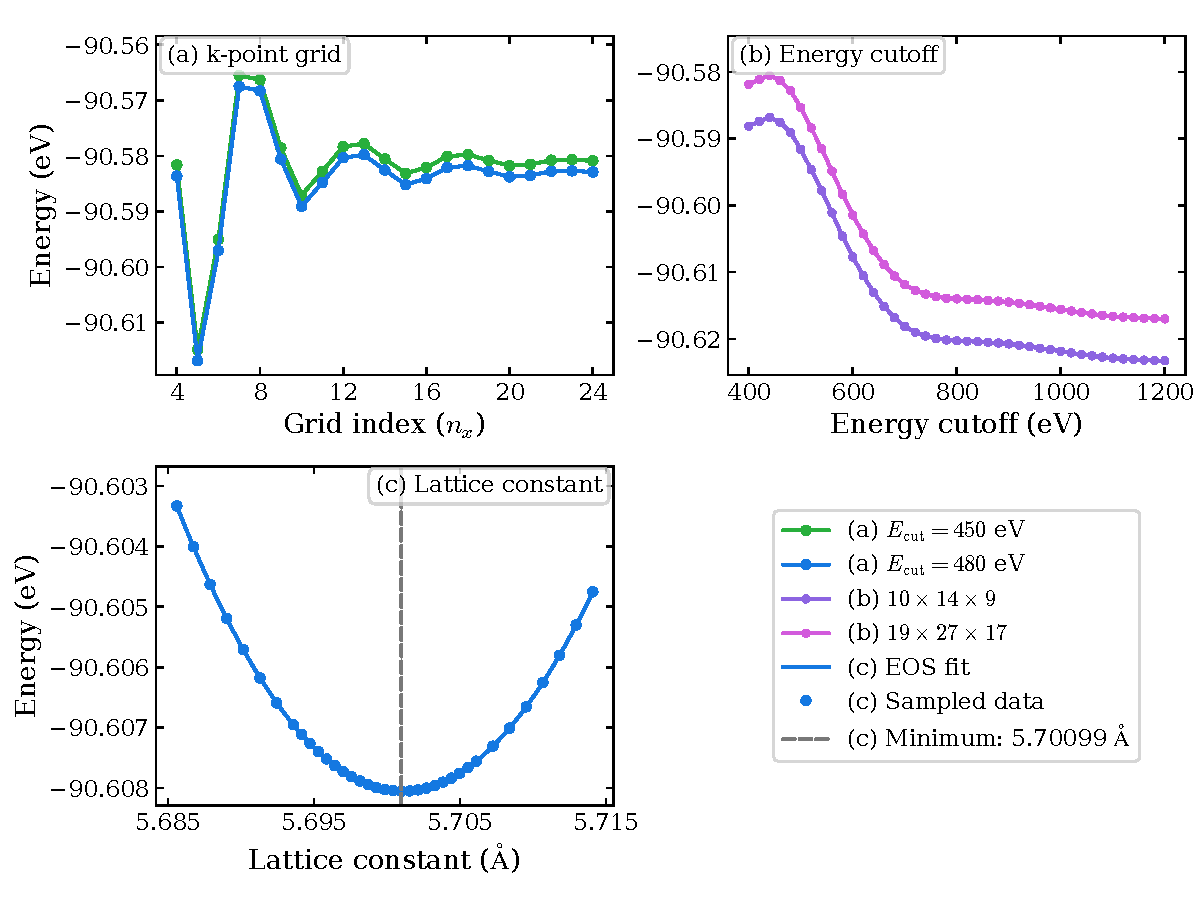
\includegraphics[width=0.80\textwidth]{figures_proj2/S2.1.pdf}
\caption[Total-energy convergence and lattice-constant scan for bulk o-\ce{B14}.]{The left panel shows the total-energy convergence of bulk o-\ce{B14} with respect to the k-point mesh (lower axis) and the plane-wave energy cutoff (upper axis).
Here, $n_x$ is the first integer of the k-point mesh.
The right panel shows the lattice-constant dependence at a plane-wave energy cutoff of \qty{600}{\electronvolt} and a k-point set of $10\times14\times9$.}
\label{S2.1}
\end{figure}

\begin{figure}[!htbp]
\centering
    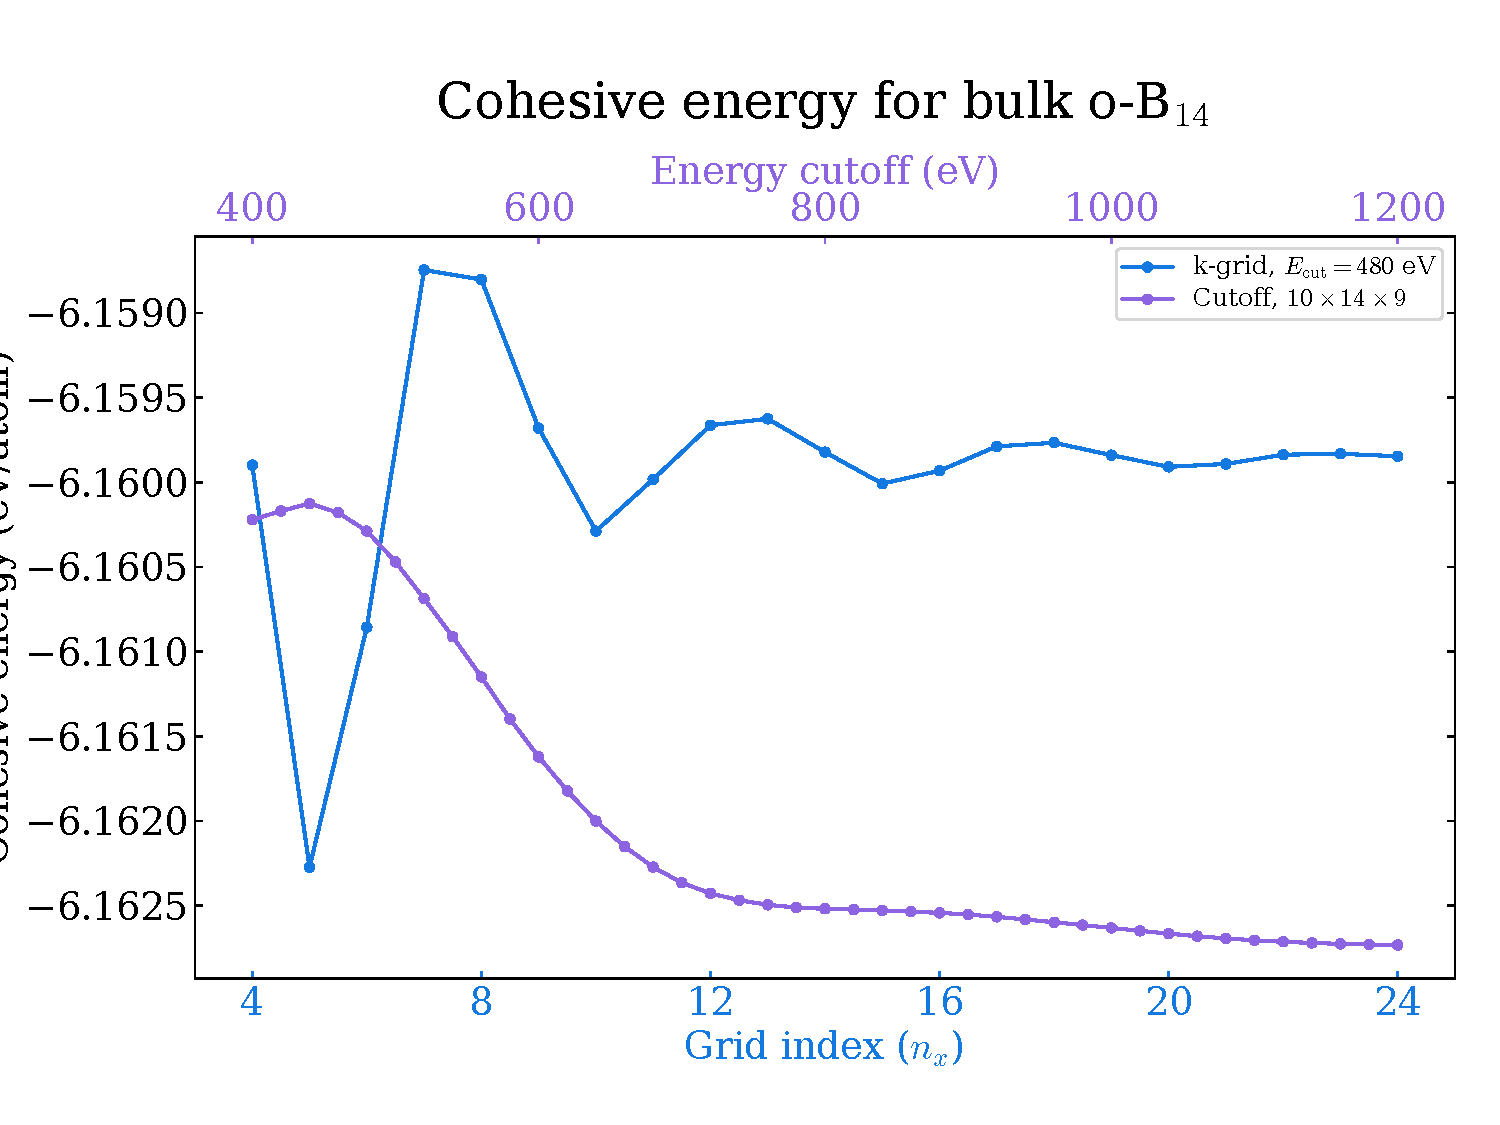
\includegraphics[width=0.60\textwidth]{figures_proj2/S2.2.pdf}
\caption{Cohesive energy per atom for bulk o-\ce{B14} as a function of the k-point mesh (lower axis) and plane-wave energy cutoff (upper axis).
Here, $n_x$ is the first integer of the k-point mesh.}
\label{S2.2}
\end{figure}

\begin{figure}[!htbp]
\centering
    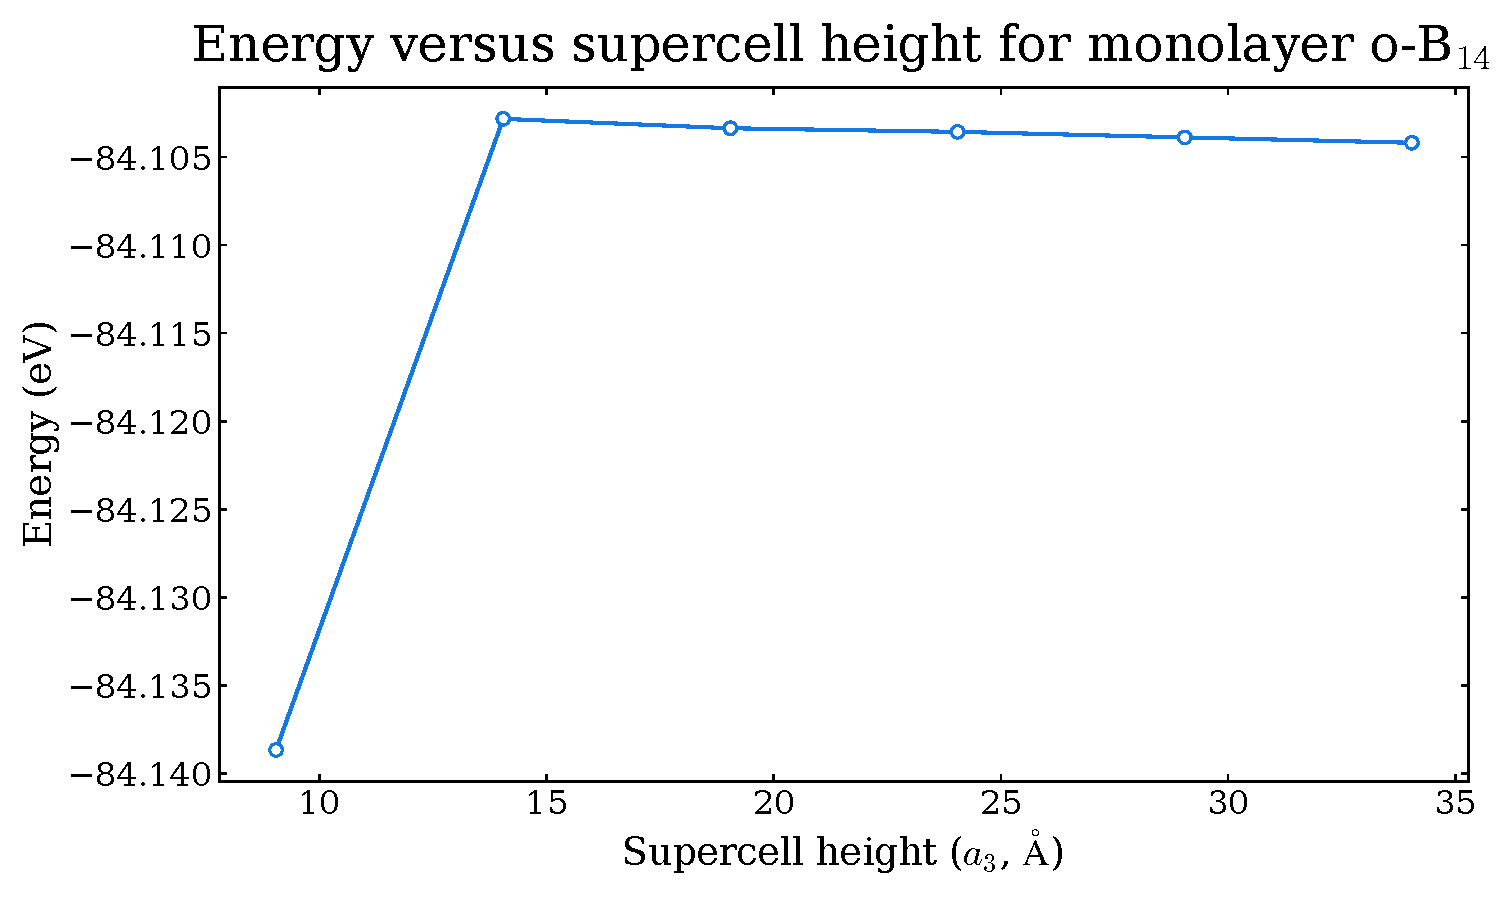
\includegraphics[width=0.60\textwidth]{figures_proj2/S2.3.pdf}
\caption{Total energy as a function of the supercell length $a_3$ normal to the layers.}
\label{S2.3}
\end{figure}

\begin{figure}[!htbp]
\centering
    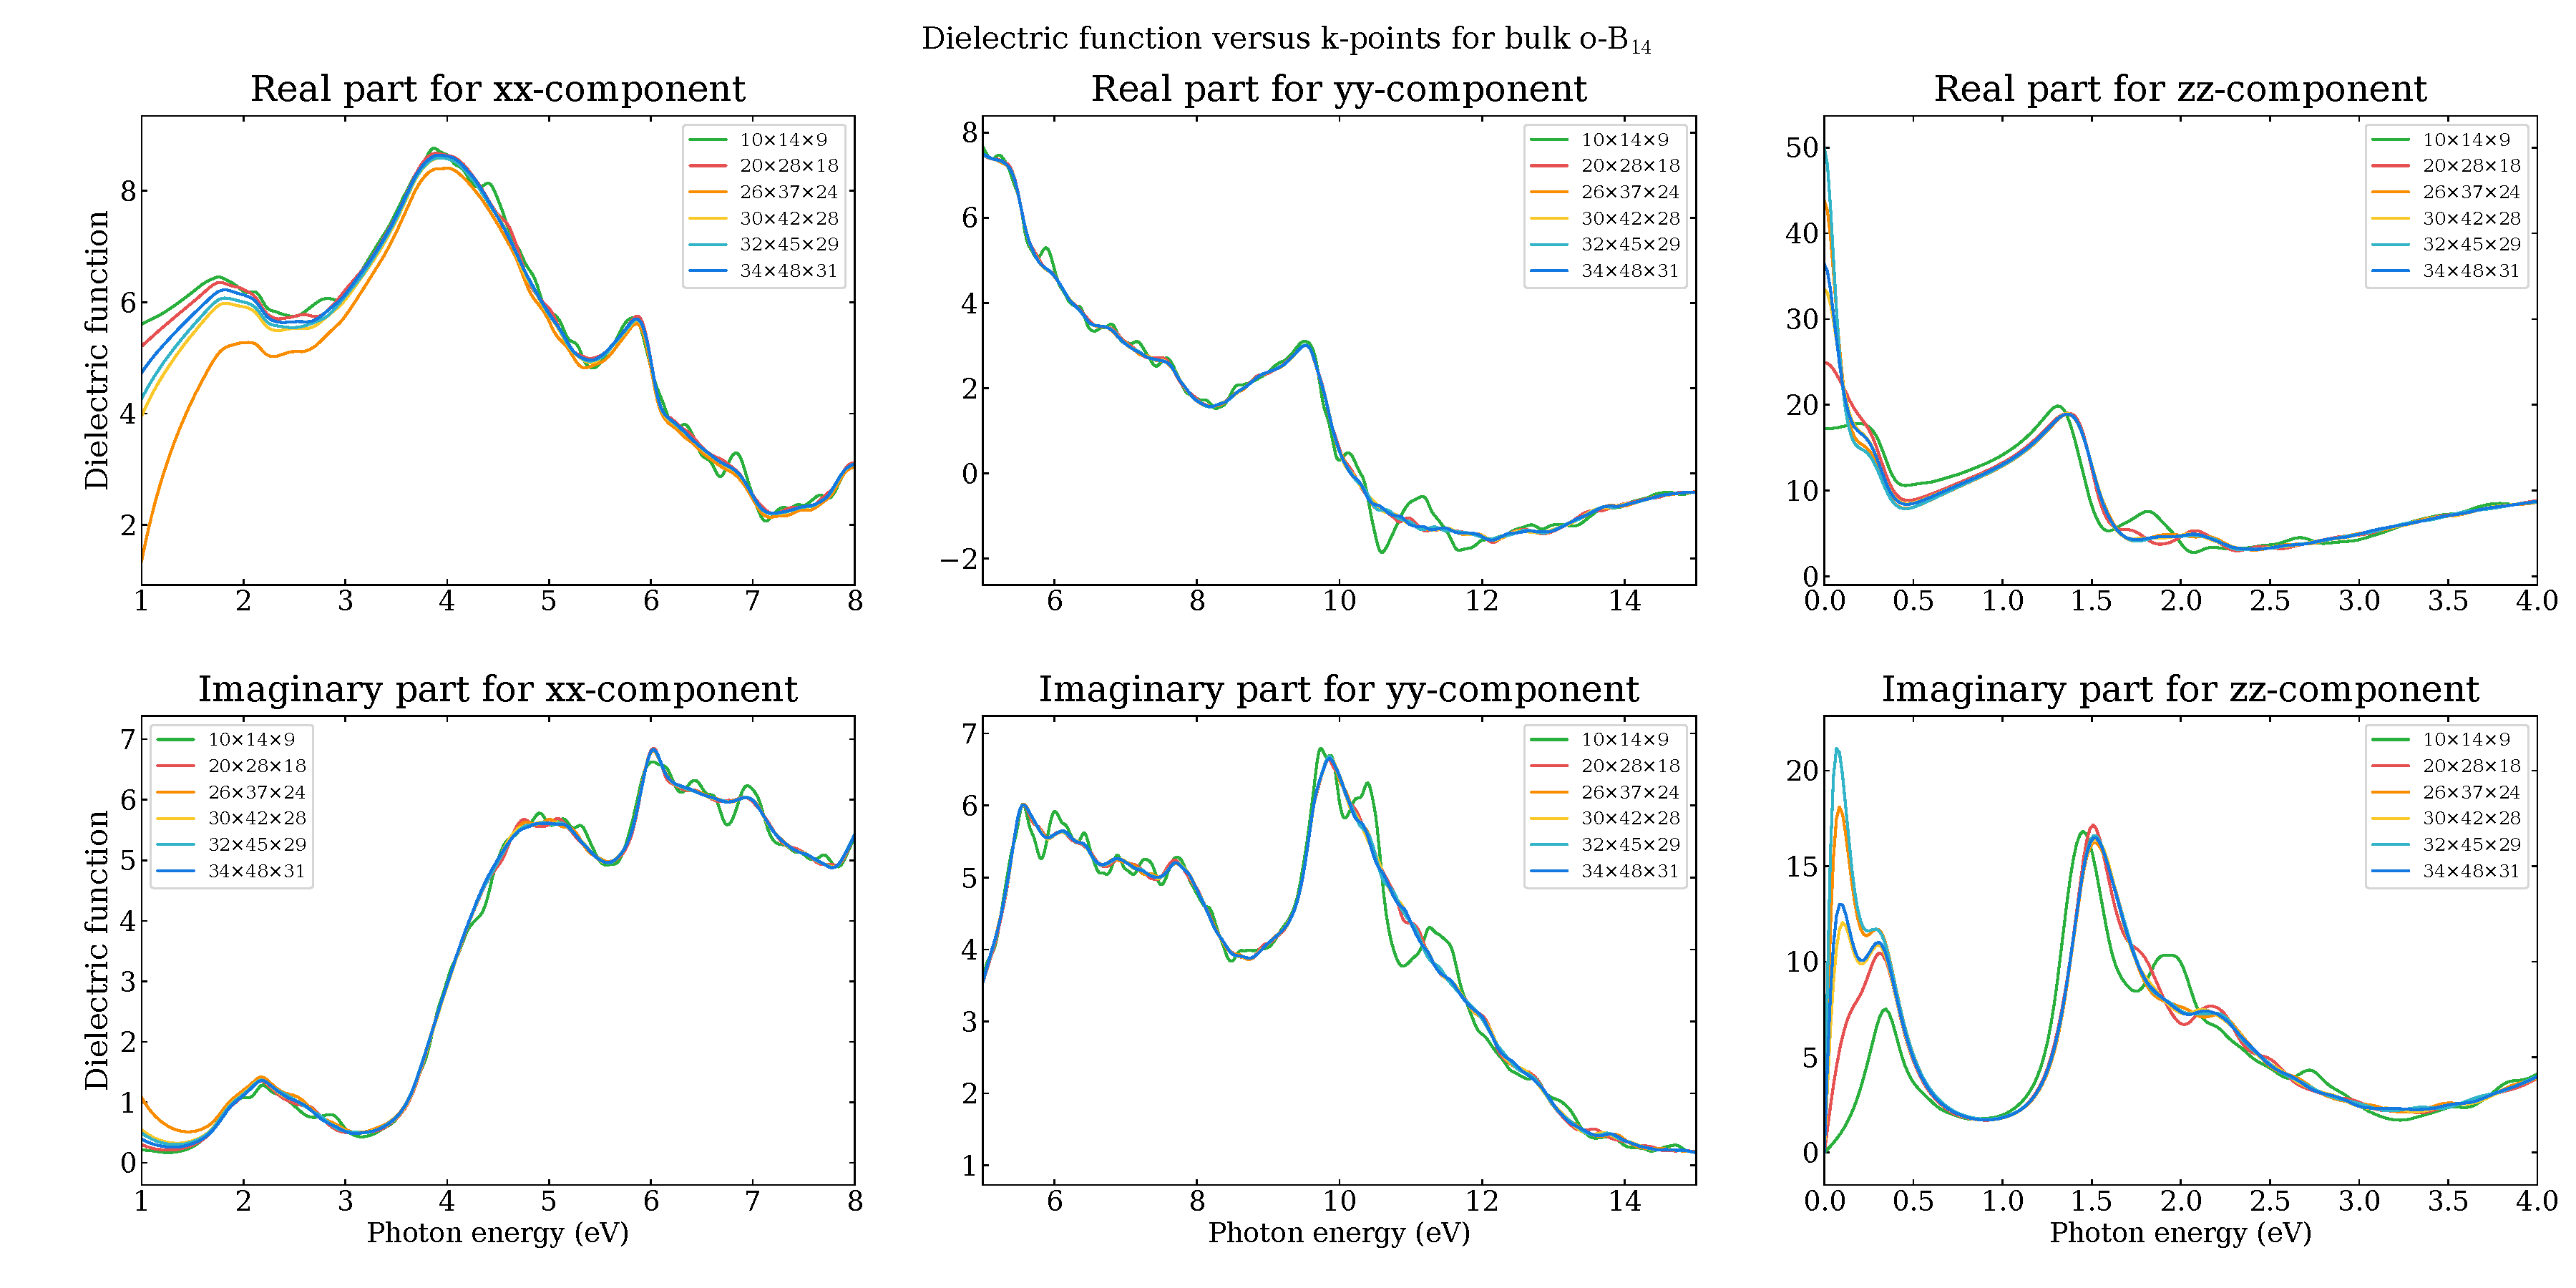
\includegraphics[width=1.00\textwidth]{figures_proj2/S2.4.pdf}
\caption{In-plane and out-of-plane components of the real and imaginary parts of the dielectric function of o-\ce{B14},
calculated with various k-point sets.}
\label{S2.4}
\end{figure}

\begin{figure}[!htbp]
\centering
    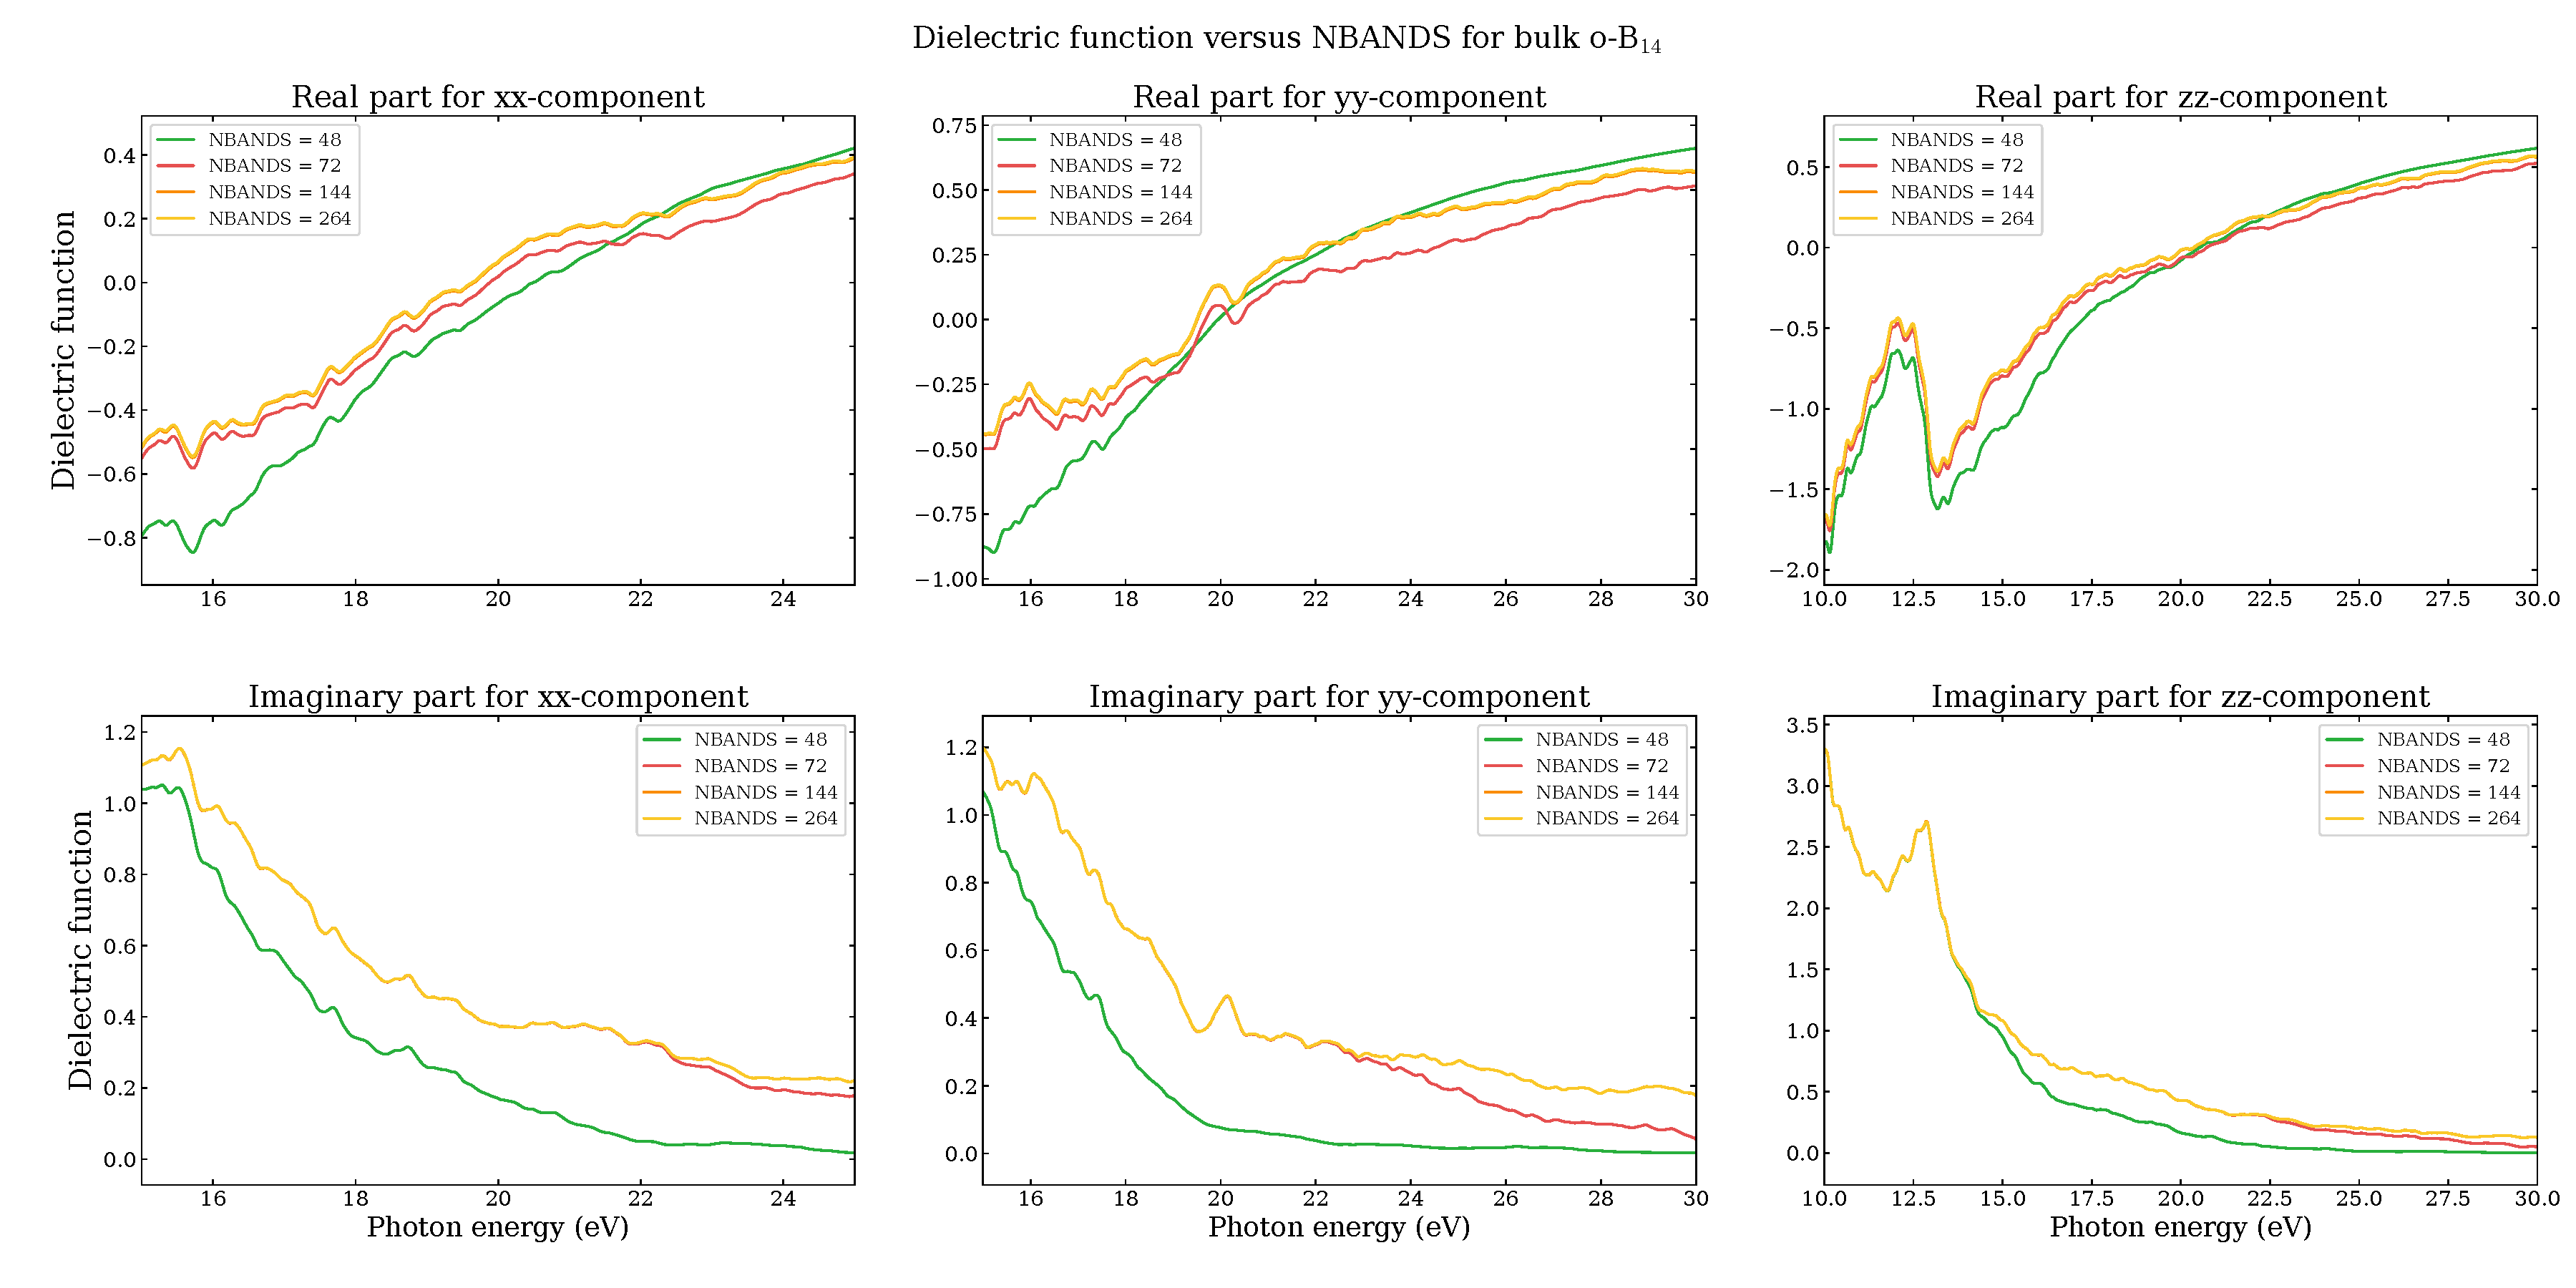
\includegraphics[width=1.00\textwidth]{figures_proj2/S2.5.pdf}
\caption[Dielectric-function convergence with the number of bands for bulk o-\ce{B14}.]{In-plane and out-of-plane components of the real and imaginary parts of the dielectric function of bulk o-\ce{B14},
calculated with different total numbers of bands.
The legend gives the actual numbers used by \texttt{VASP}; the requested \texttt{NBANDS} values were 32, 64, 128, and 256, respectively.
Both occupied and unoccupied states are included.}
\label{S2.5}
\end{figure}

\begin{figure}[!htbp]
\centering
    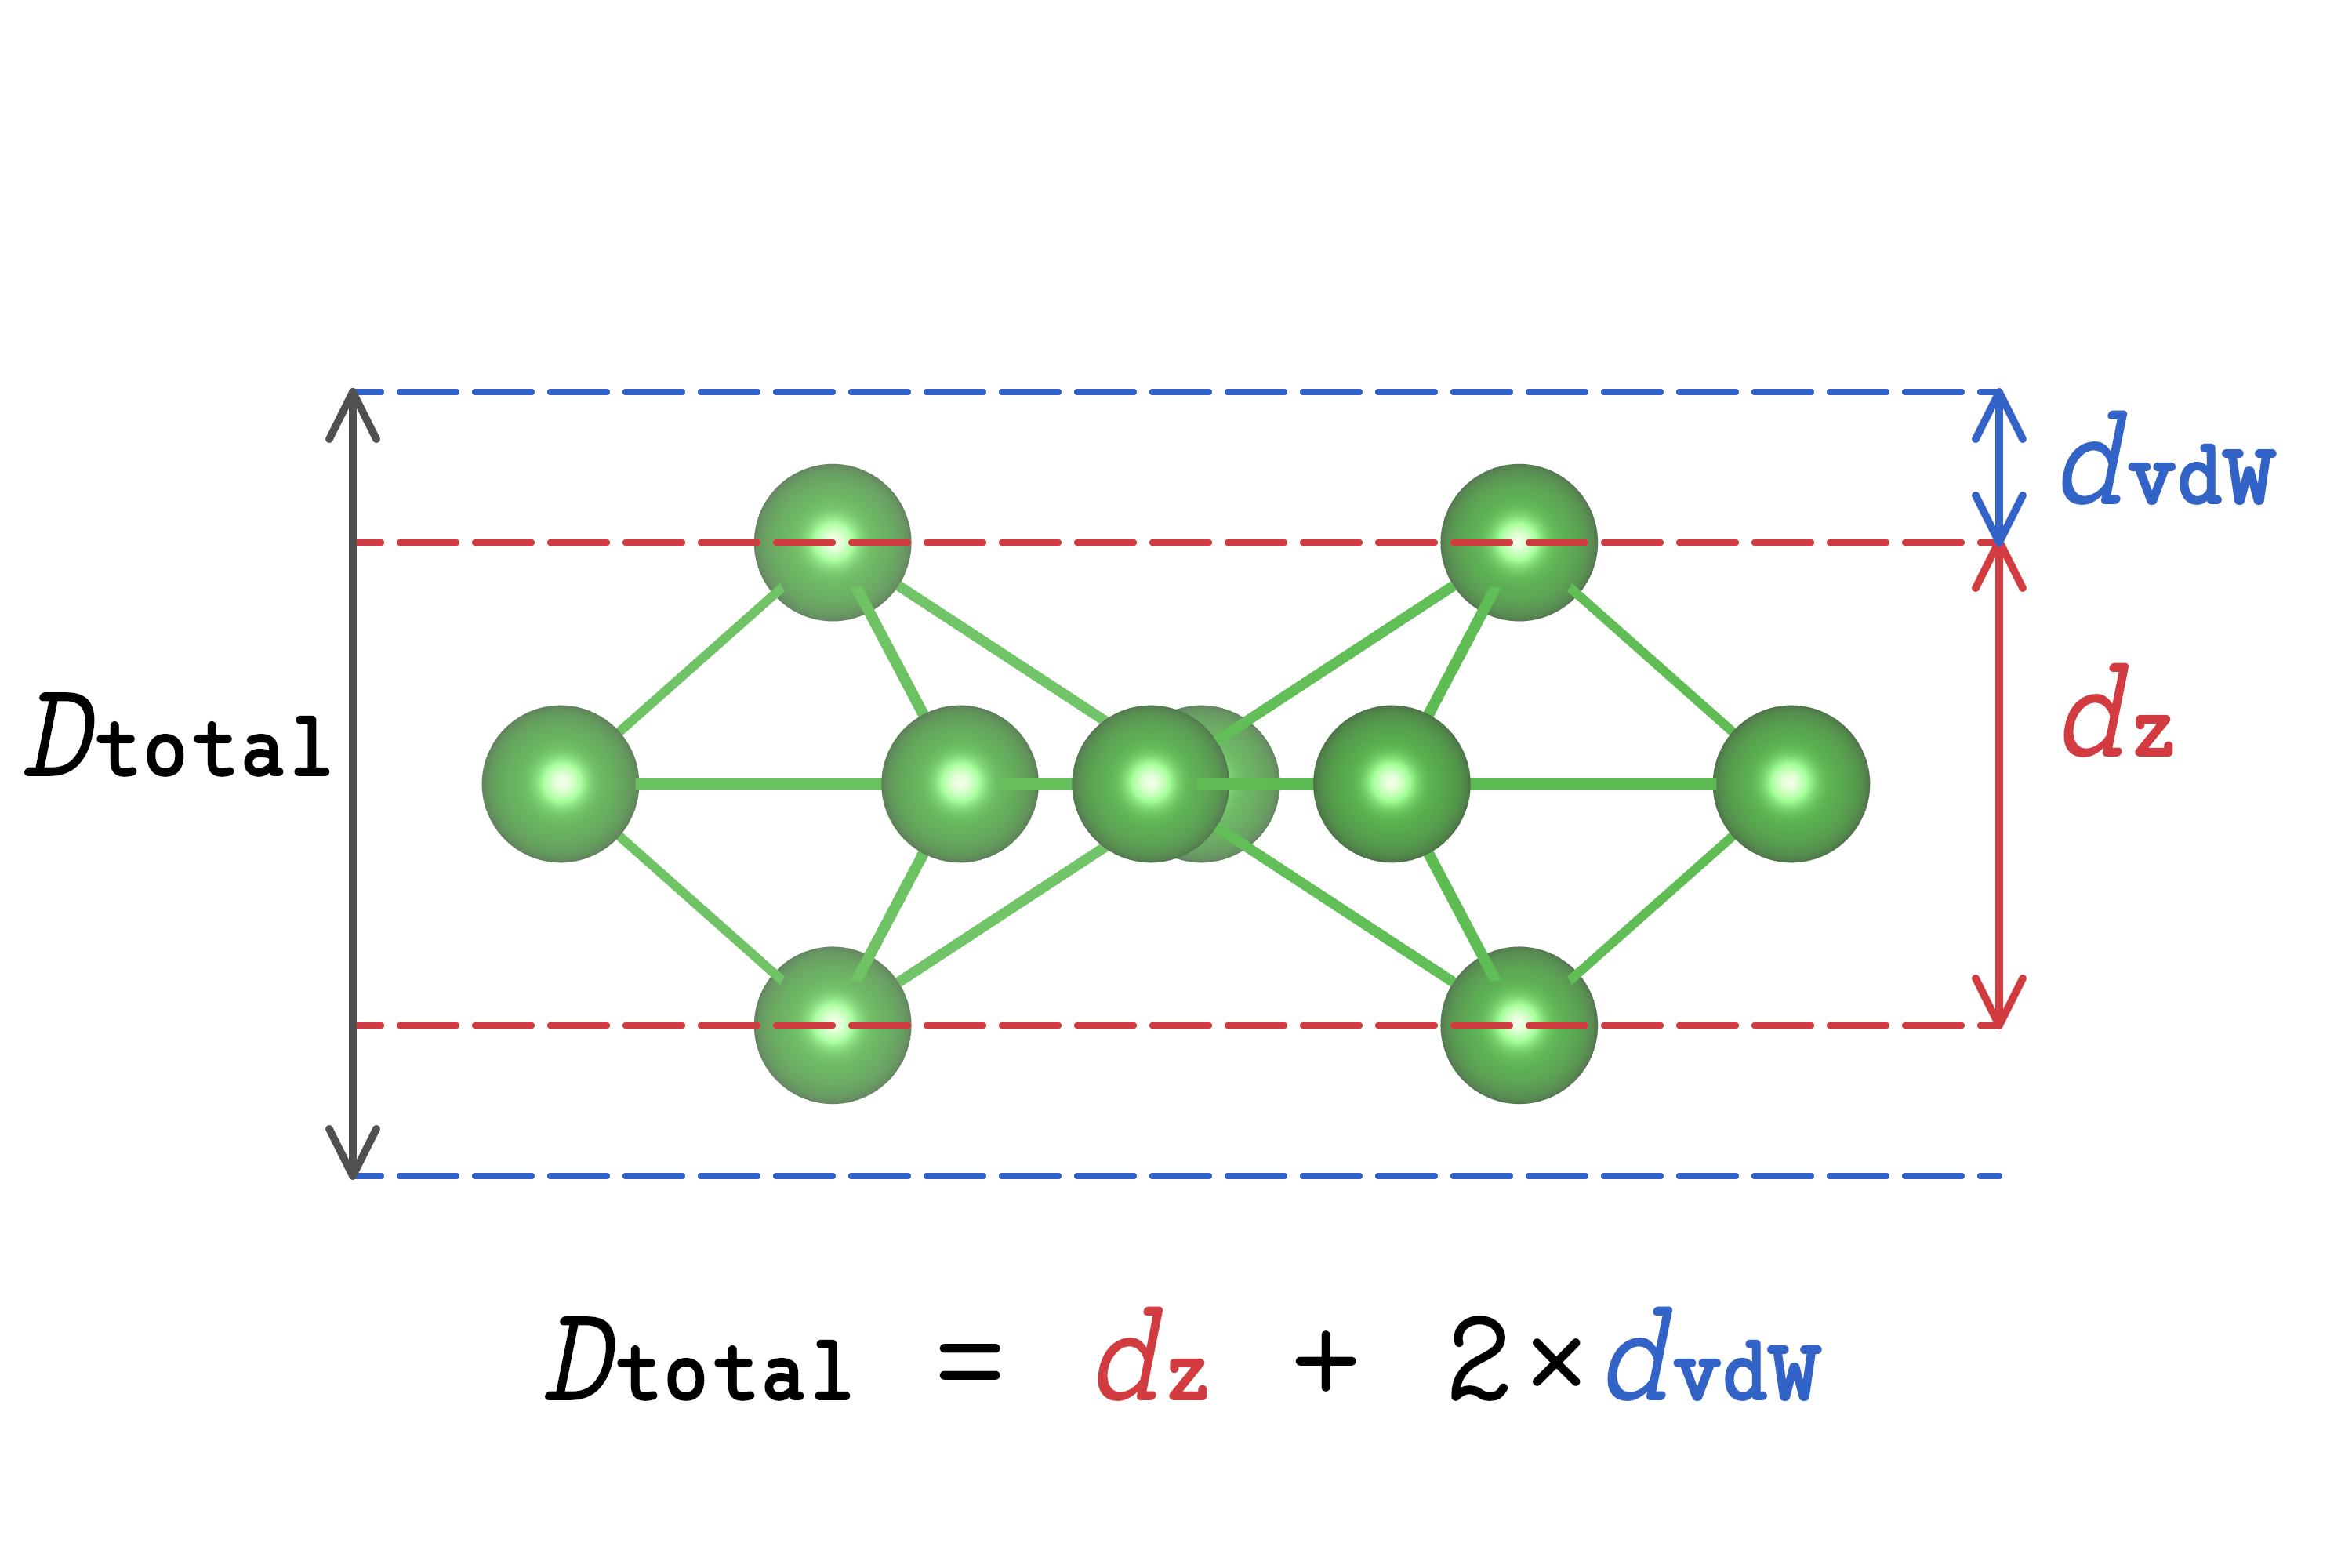
\includegraphics[width=0.60\textwidth]{figures_proj2/S2.6.png}
\caption{Definition of the layer thickness used in the renormalization of the dielectric function, $D_{\mathrm{total}} \coloneqq d_{\mathrm{2D}}$.}
\label{S2.6}
\end{figure}

\begin{figure}[!htbp]
\centering
    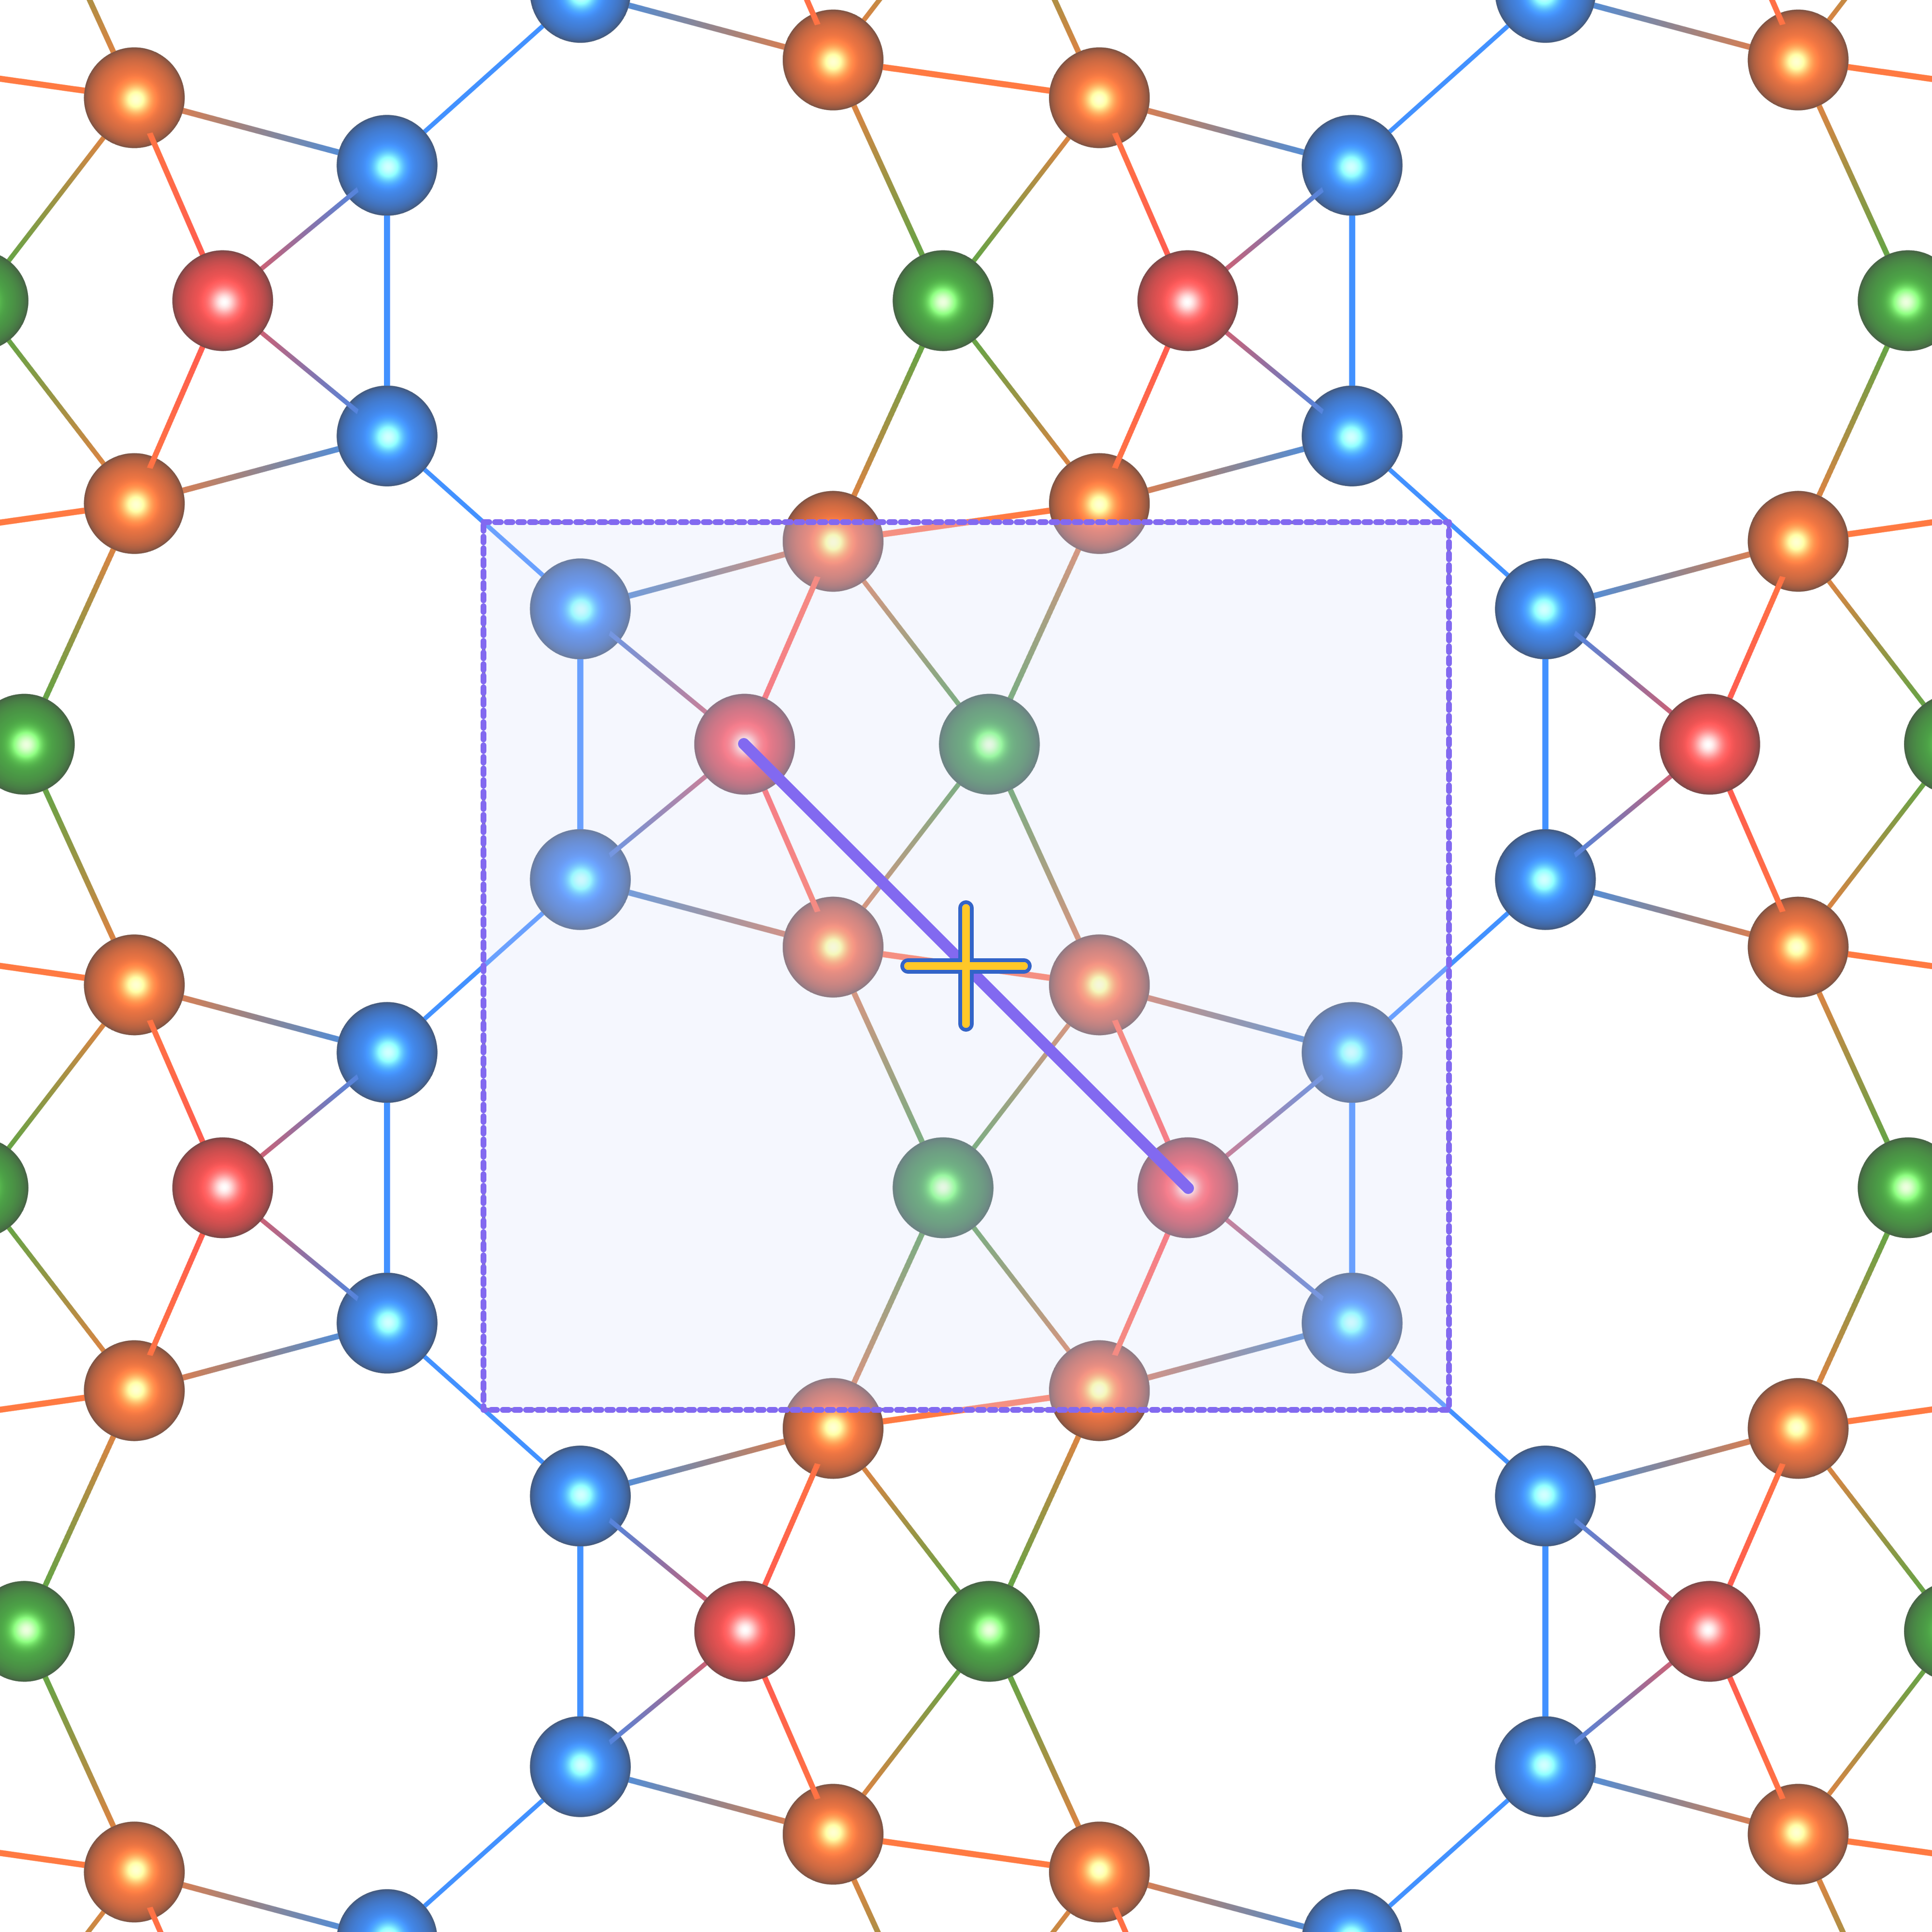
\includegraphics[width=0.60\textwidth]{figures_proj2/S2.7.png}
\caption{Sketch of the hollow-bridge site, indicated by the yellow cross,
for the hydrogen adsorption on the monolayer and bilayer structures.
The black rectangle represents the unit cell.}
\label{S2.7}
\end{figure}

\begin{figure}[!htbp]
\centering
    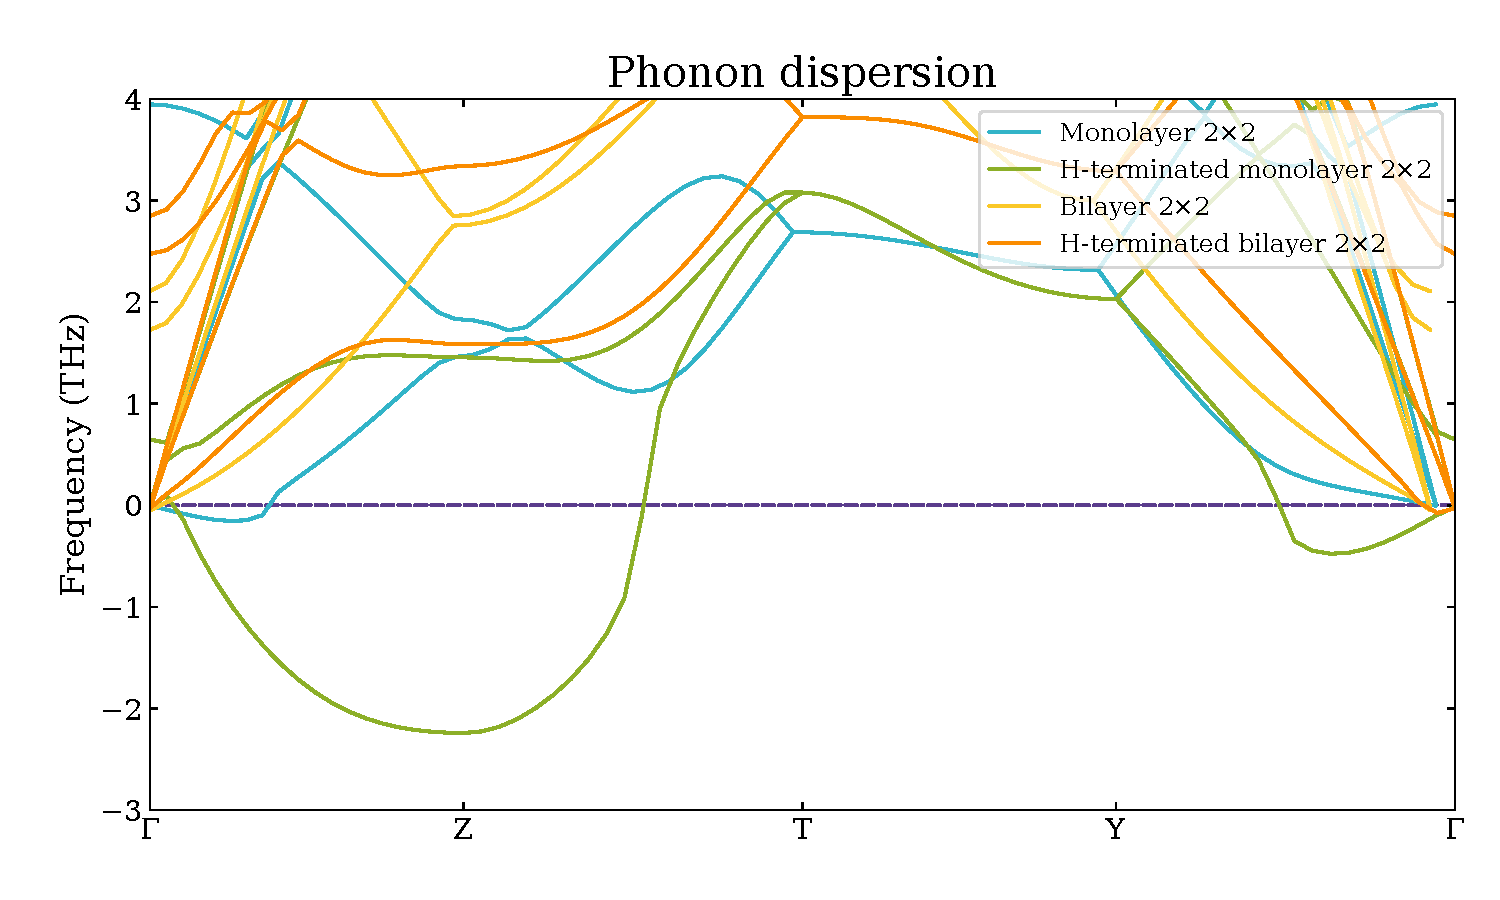
\includegraphics[width=0.60\textwidth]{figures_proj2/S2.8.pdf}
\caption{Phonon-dispersion curves obtained using a $(2\times2)$ supercell.}
\label{S2.8}
\end{figure}

\begin{figure}[!htbp]
\centering
    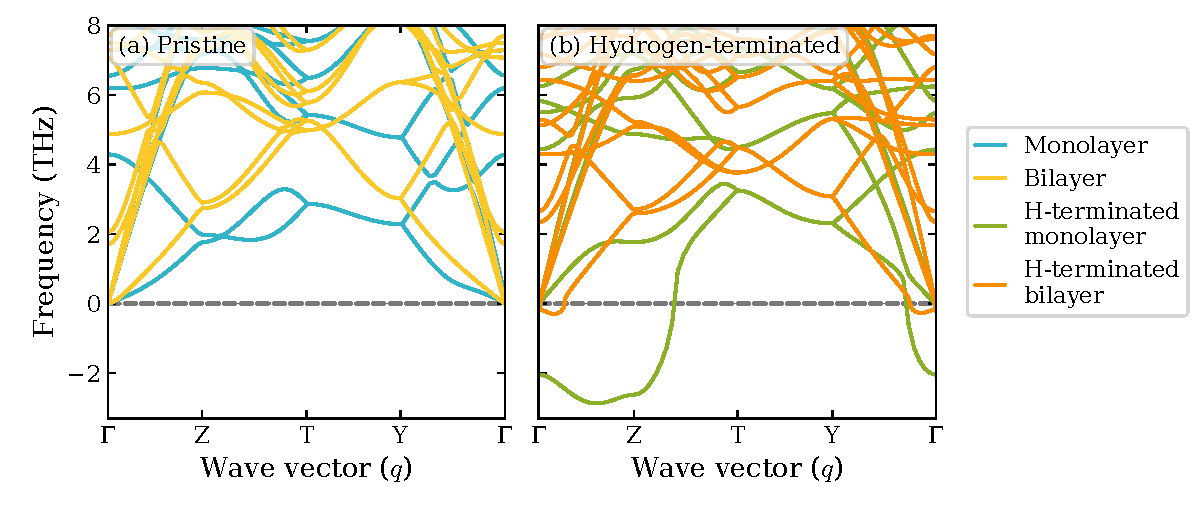
\includegraphics[width=0.80\textwidth]{figures_proj2/S2.9.pdf}
\caption{Left: Phonon-dispersion curves of the monolayer and bilayer calculated using a $3\times3$ supercell;
Right: Phonon-dispersion curves of the hydrogen-terminated monolayer and bilayer calculated using a $3\times3$ supercell.
Small imaginary frequencies appear around the $\Gamma$ point for the hydrogen-terminated bilayer.
Such modes can be sensitive to numerical convergence in two-dimensional materials~\cite{liu2016continuum,querne2023crystal,pallikara2022physical},
and a physical instability is the alternative explanation.}
\label{S2.9}
\end{figure}

\begin{figure}[!htbp]
\centering
    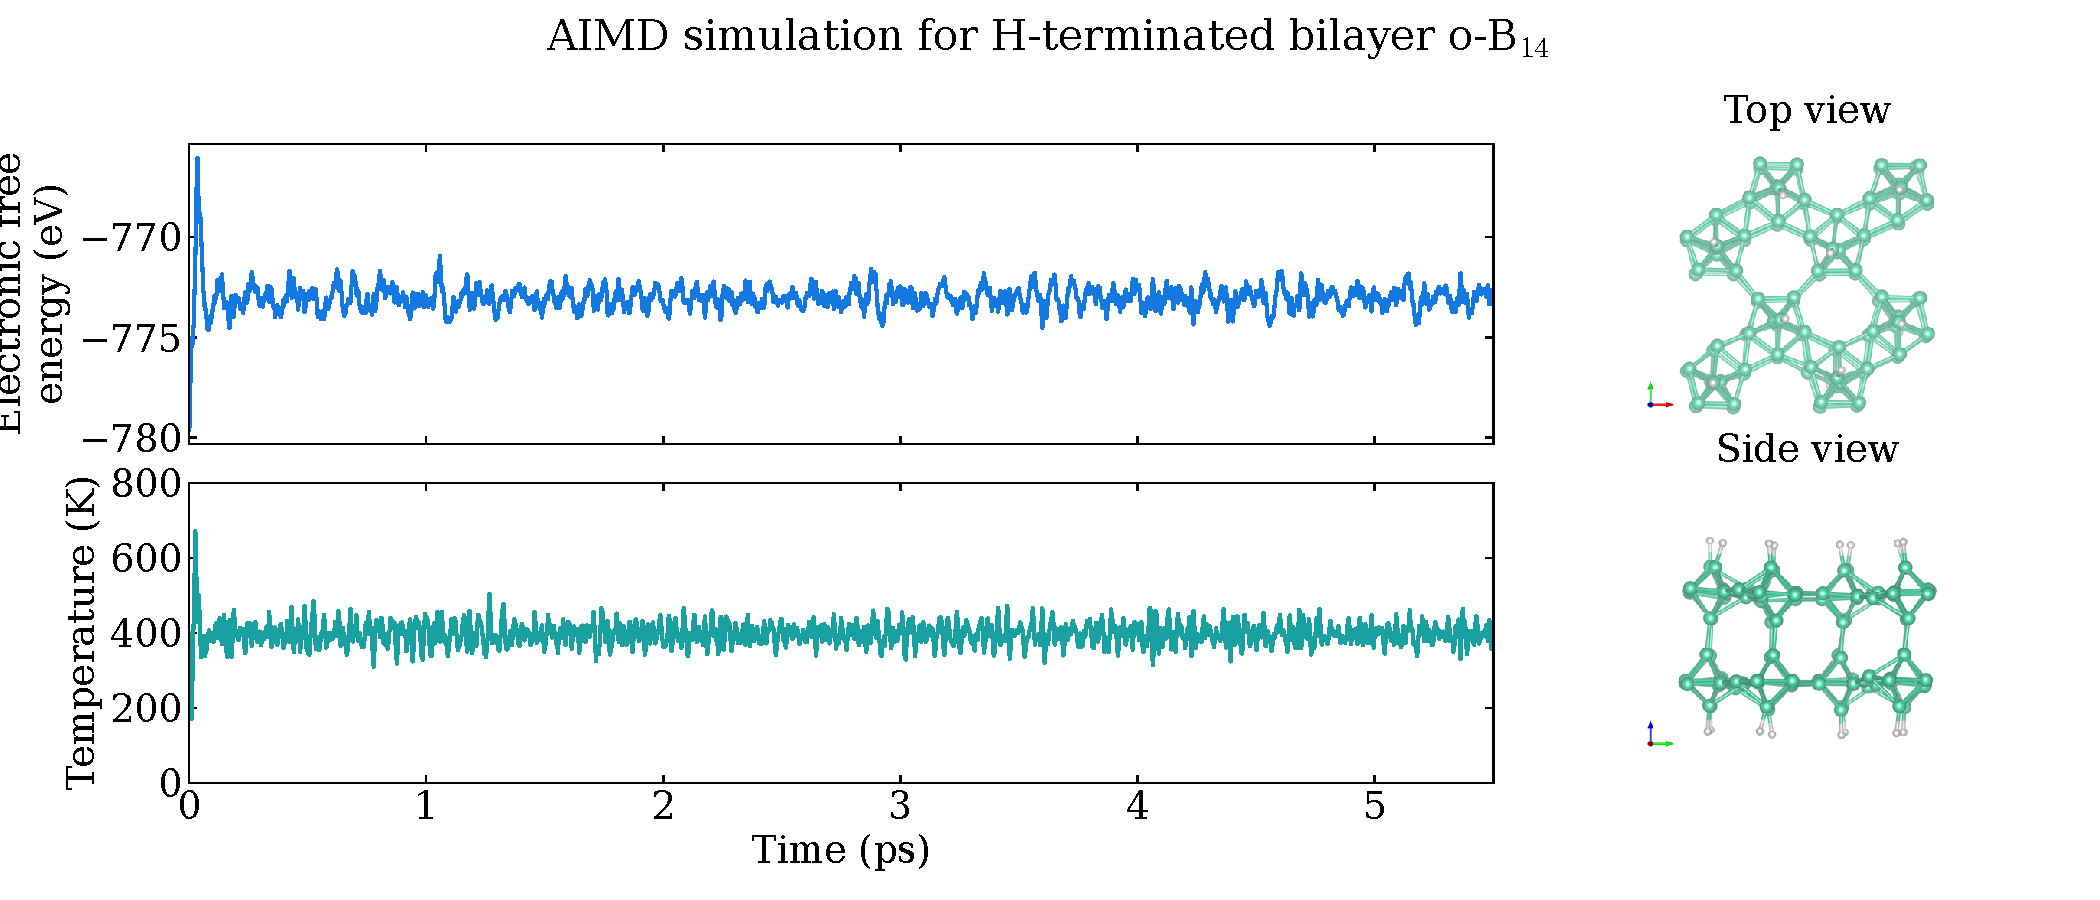
\includegraphics[width=0.80\textwidth]{figures_proj2/S2.10.pdf}
\caption{
Left: Electronic free energy and temperature as functions of time from \textit{ab initio} molecular dynamics calculations for the hydrogen-terminated bilayer at \qty{400}{K};
Right: Top and side views of the molecular structure of the hydrogen-terminated bilayer at the corresponding temperature.
The bonding framework persists over the \qty{5.5}{ps} trajectory in the NVT ensemble.}
\label{S2.10}
\end{figure}

\begin{figure}[!htbp]
\centering
    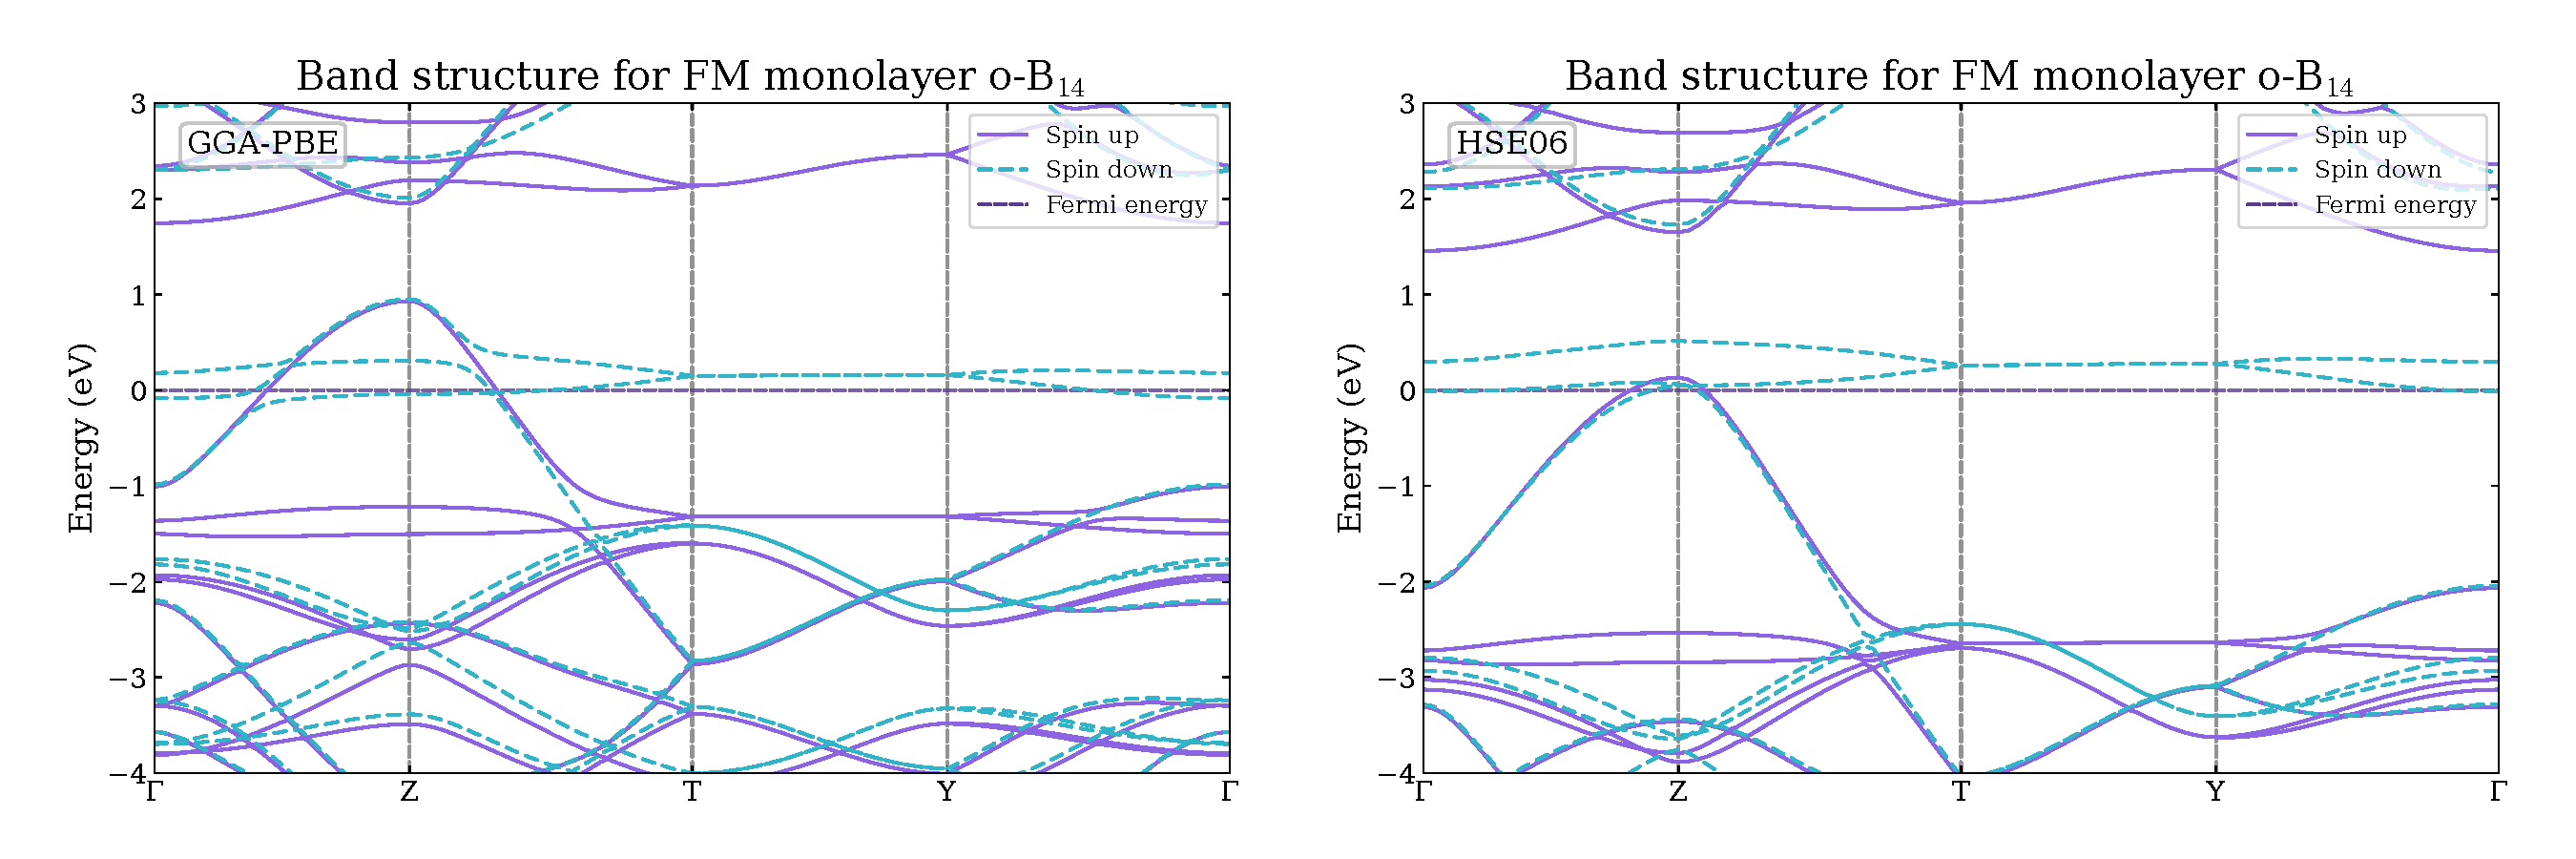
\includegraphics[width=0.80\textwidth]{figures_proj2/S2.11.pdf}
\caption{
Left: Spin-polarized ferromagnetic band structure of the monolayer calculated using the PBE functional;
Right: Spin-polarized ferromagnetic band structure of the monolayer calculated using the HSE06 functional.}
\label{S2.11}
\end{figure}

\begin{figure}[!htbp]
\centering
    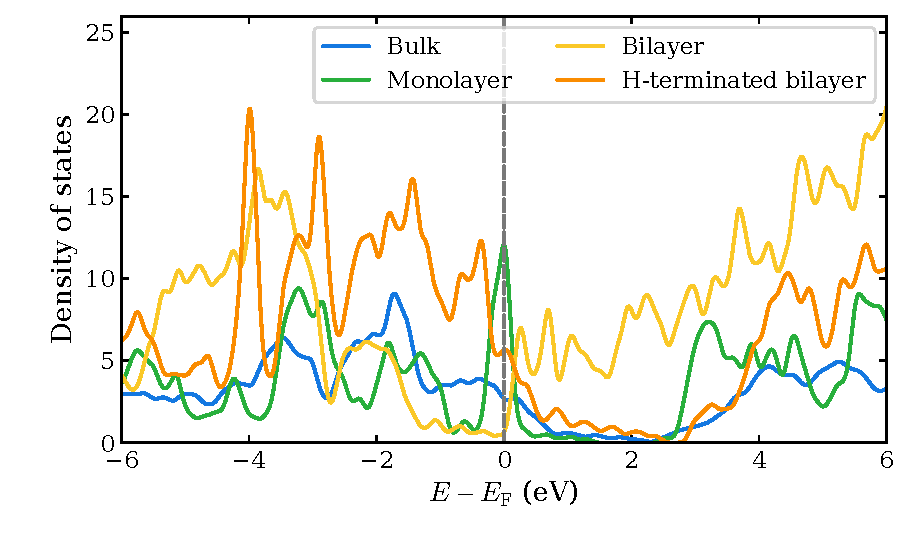
\includegraphics[width=0.60\textwidth]{figures_proj2/S2.12.pdf}
\caption{Total density of states (DoS) of the various structures as calculated using the PBE functional.}
\label{S2.12}
\end{figure}

\begin{figure}[!htbp]
\centering
    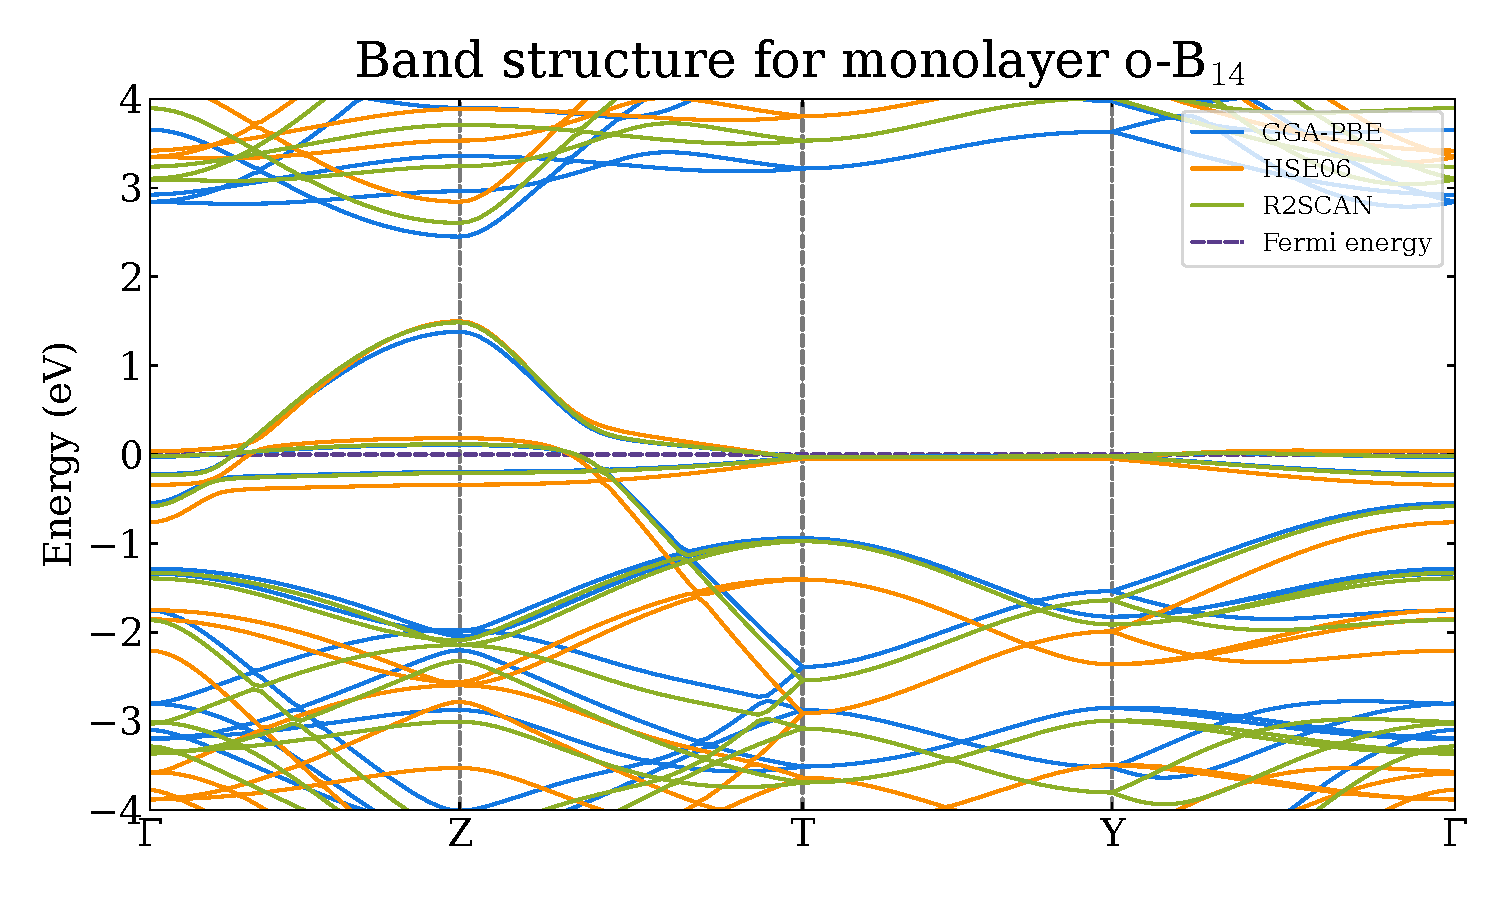
\includegraphics[width=0.60\textwidth]{figures_proj2/S2.13.pdf}
\caption{Non-spin-polarized band structure of the monolayer calculated using different functionals.}
\label{S2.13}
\end{figure}

\begin{figure}[!htbp]
\centering
    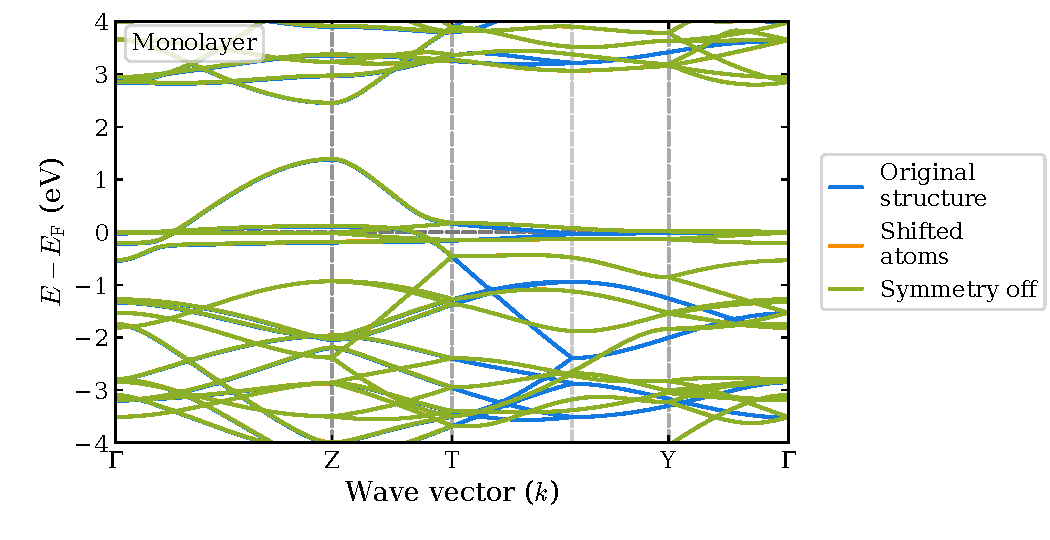
\includegraphics[width=0.60\textwidth]{figures_proj2/S2.14.pdf}
\caption{
Band structure of the monolayer calculated using a $(2\times1)$ unit cell.
The label ``shifted atoms'' means that,
in the initial atomic structure,
some atoms were moved slightly away from the ideal high-symmetry sites to break symmetry and allow Jahn--Teller distortions if they were favourable.
The structure was subsequently fully relaxed,
but the results remained unchanged and displayed no symmetry-lowering distortions.}
\label{S2.14}
\end{figure}

\begin{figure}[!htbp]
\centering
    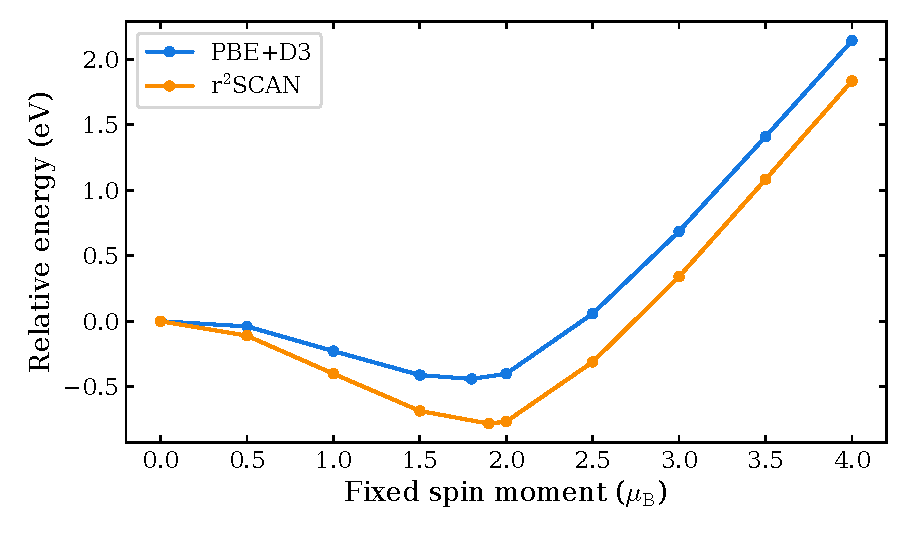
\includegraphics[width=0.60\textwidth]{figures_proj2/S2.15.pdf}
\caption{Fixed-spin energy profile of the monolayer calculated using the PBE+D3 and r$^{2}$SCAN functionals.
The relative energy reaches its minimum near a fixed spin moment of $2.0~\mu_{\mathrm{B}}$.}
\label{S2.15}
\end{figure}

\begin{figure}[!htbp]
\centering
    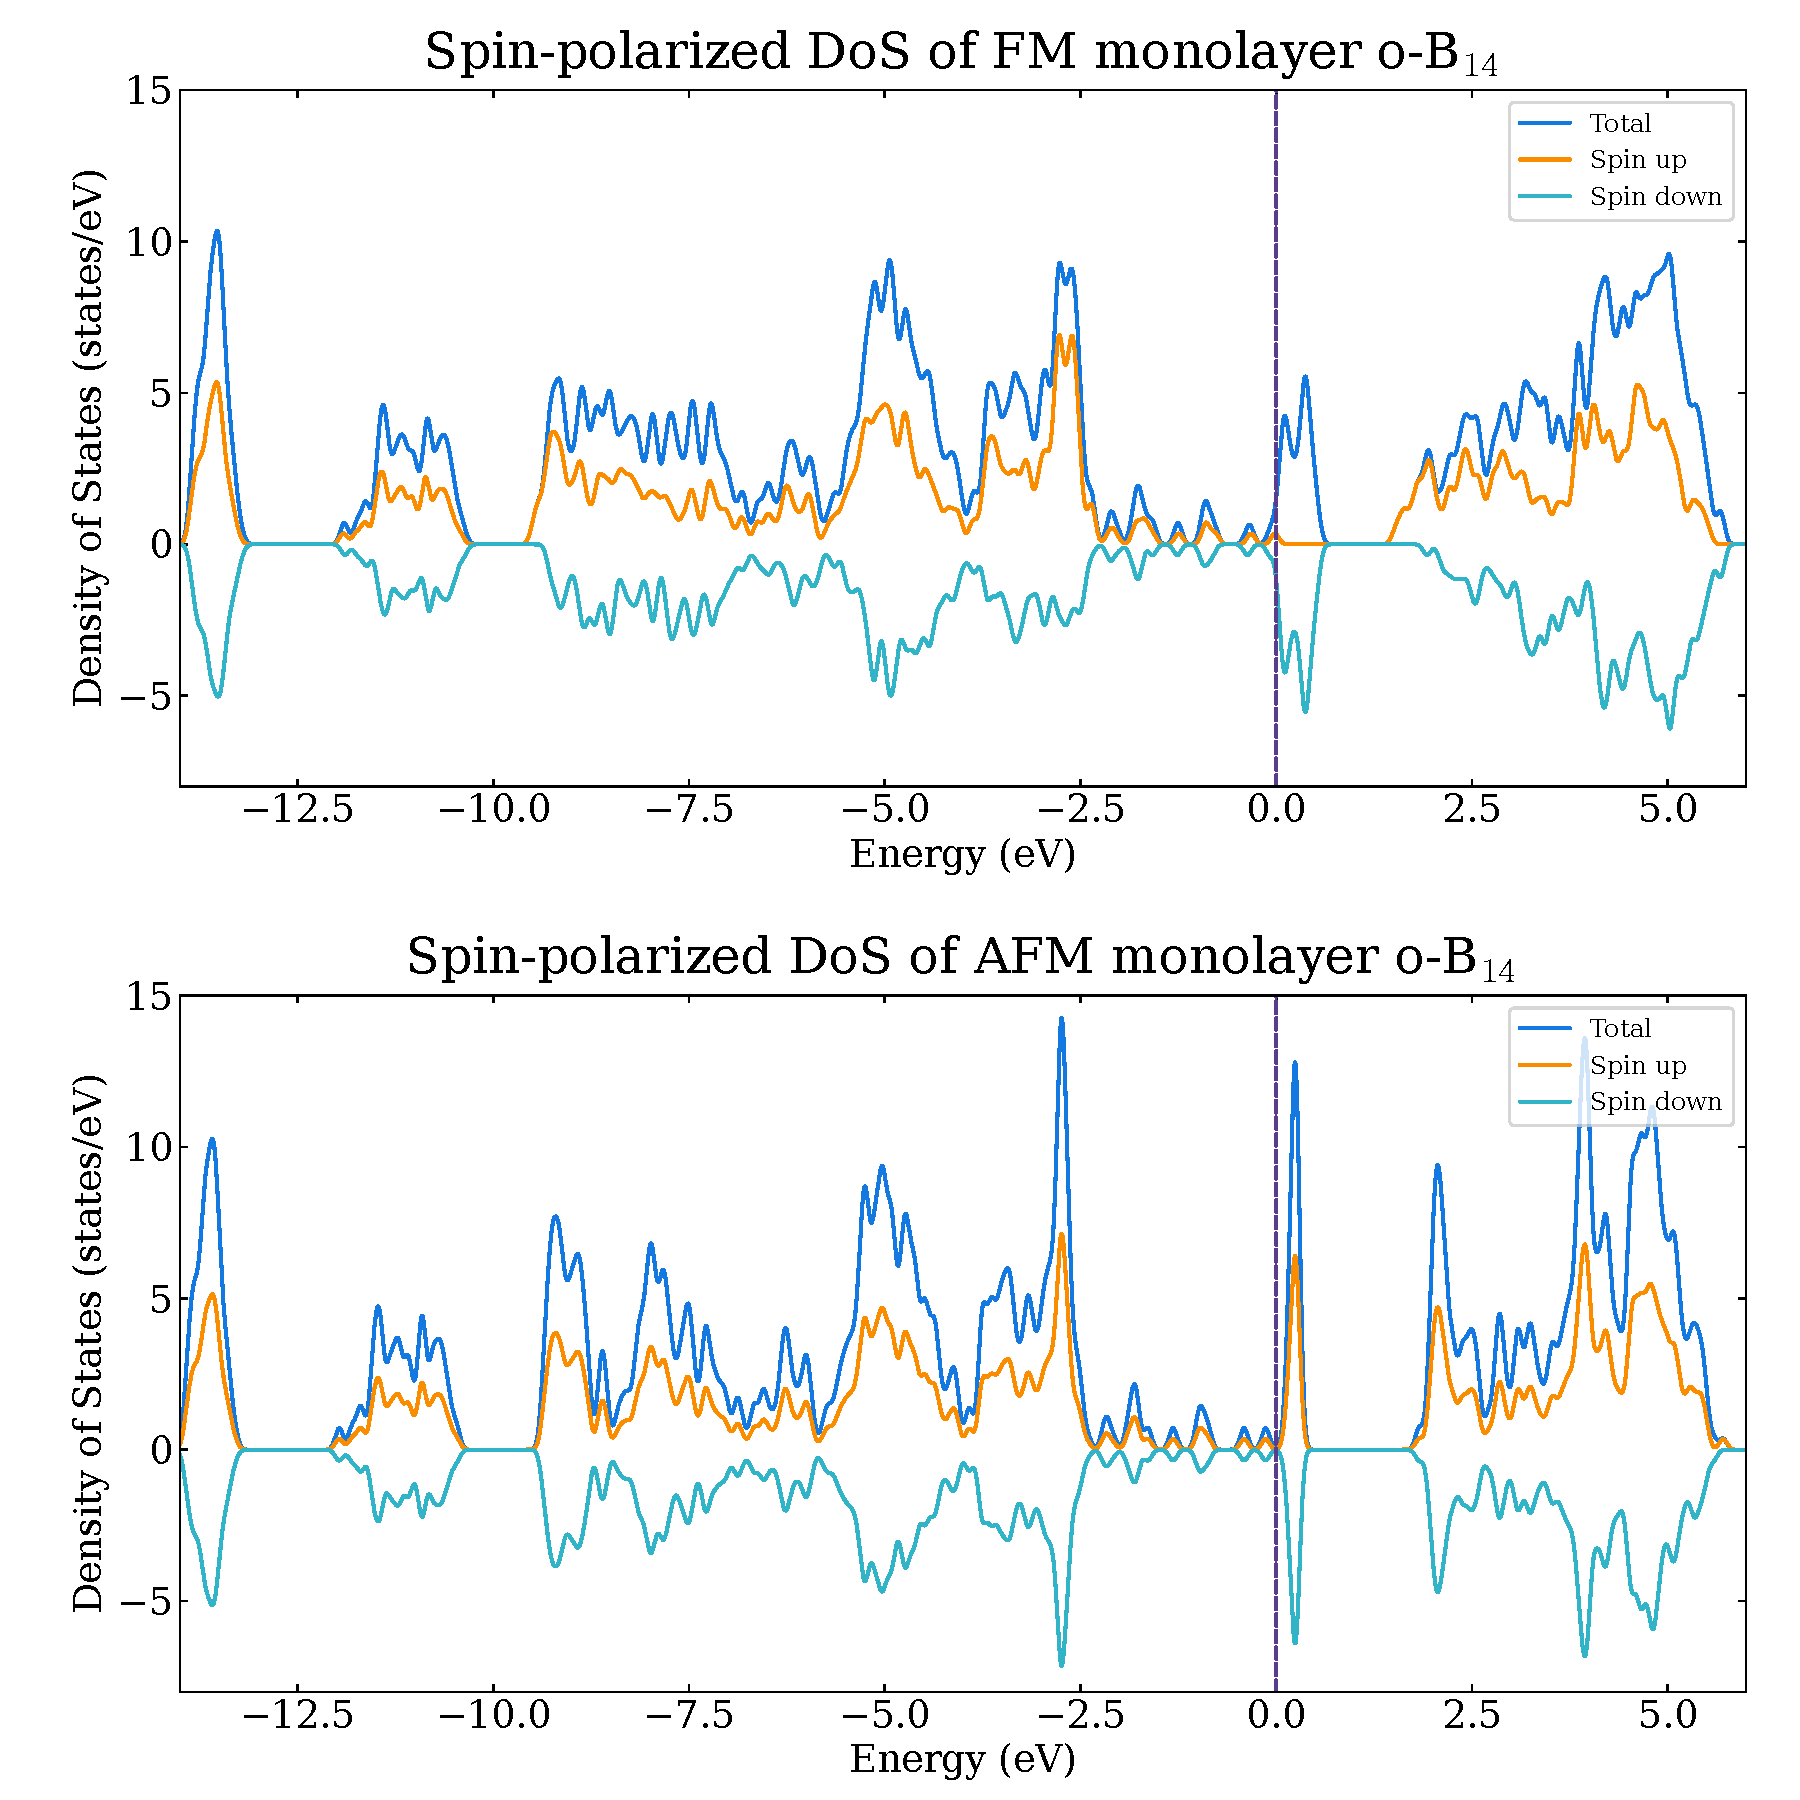
\includegraphics[width=0.60\textwidth]{figures_proj2/S2.16.pdf}
\caption{Spin-resolved total DoS for the FM monolayer (upper panel) and the AFM monolayer (lower panel),
as calculated using the HSE06 functional.}
\label{S2.16}
\end{figure}

\begin{figure}[!htbp]
\centering
    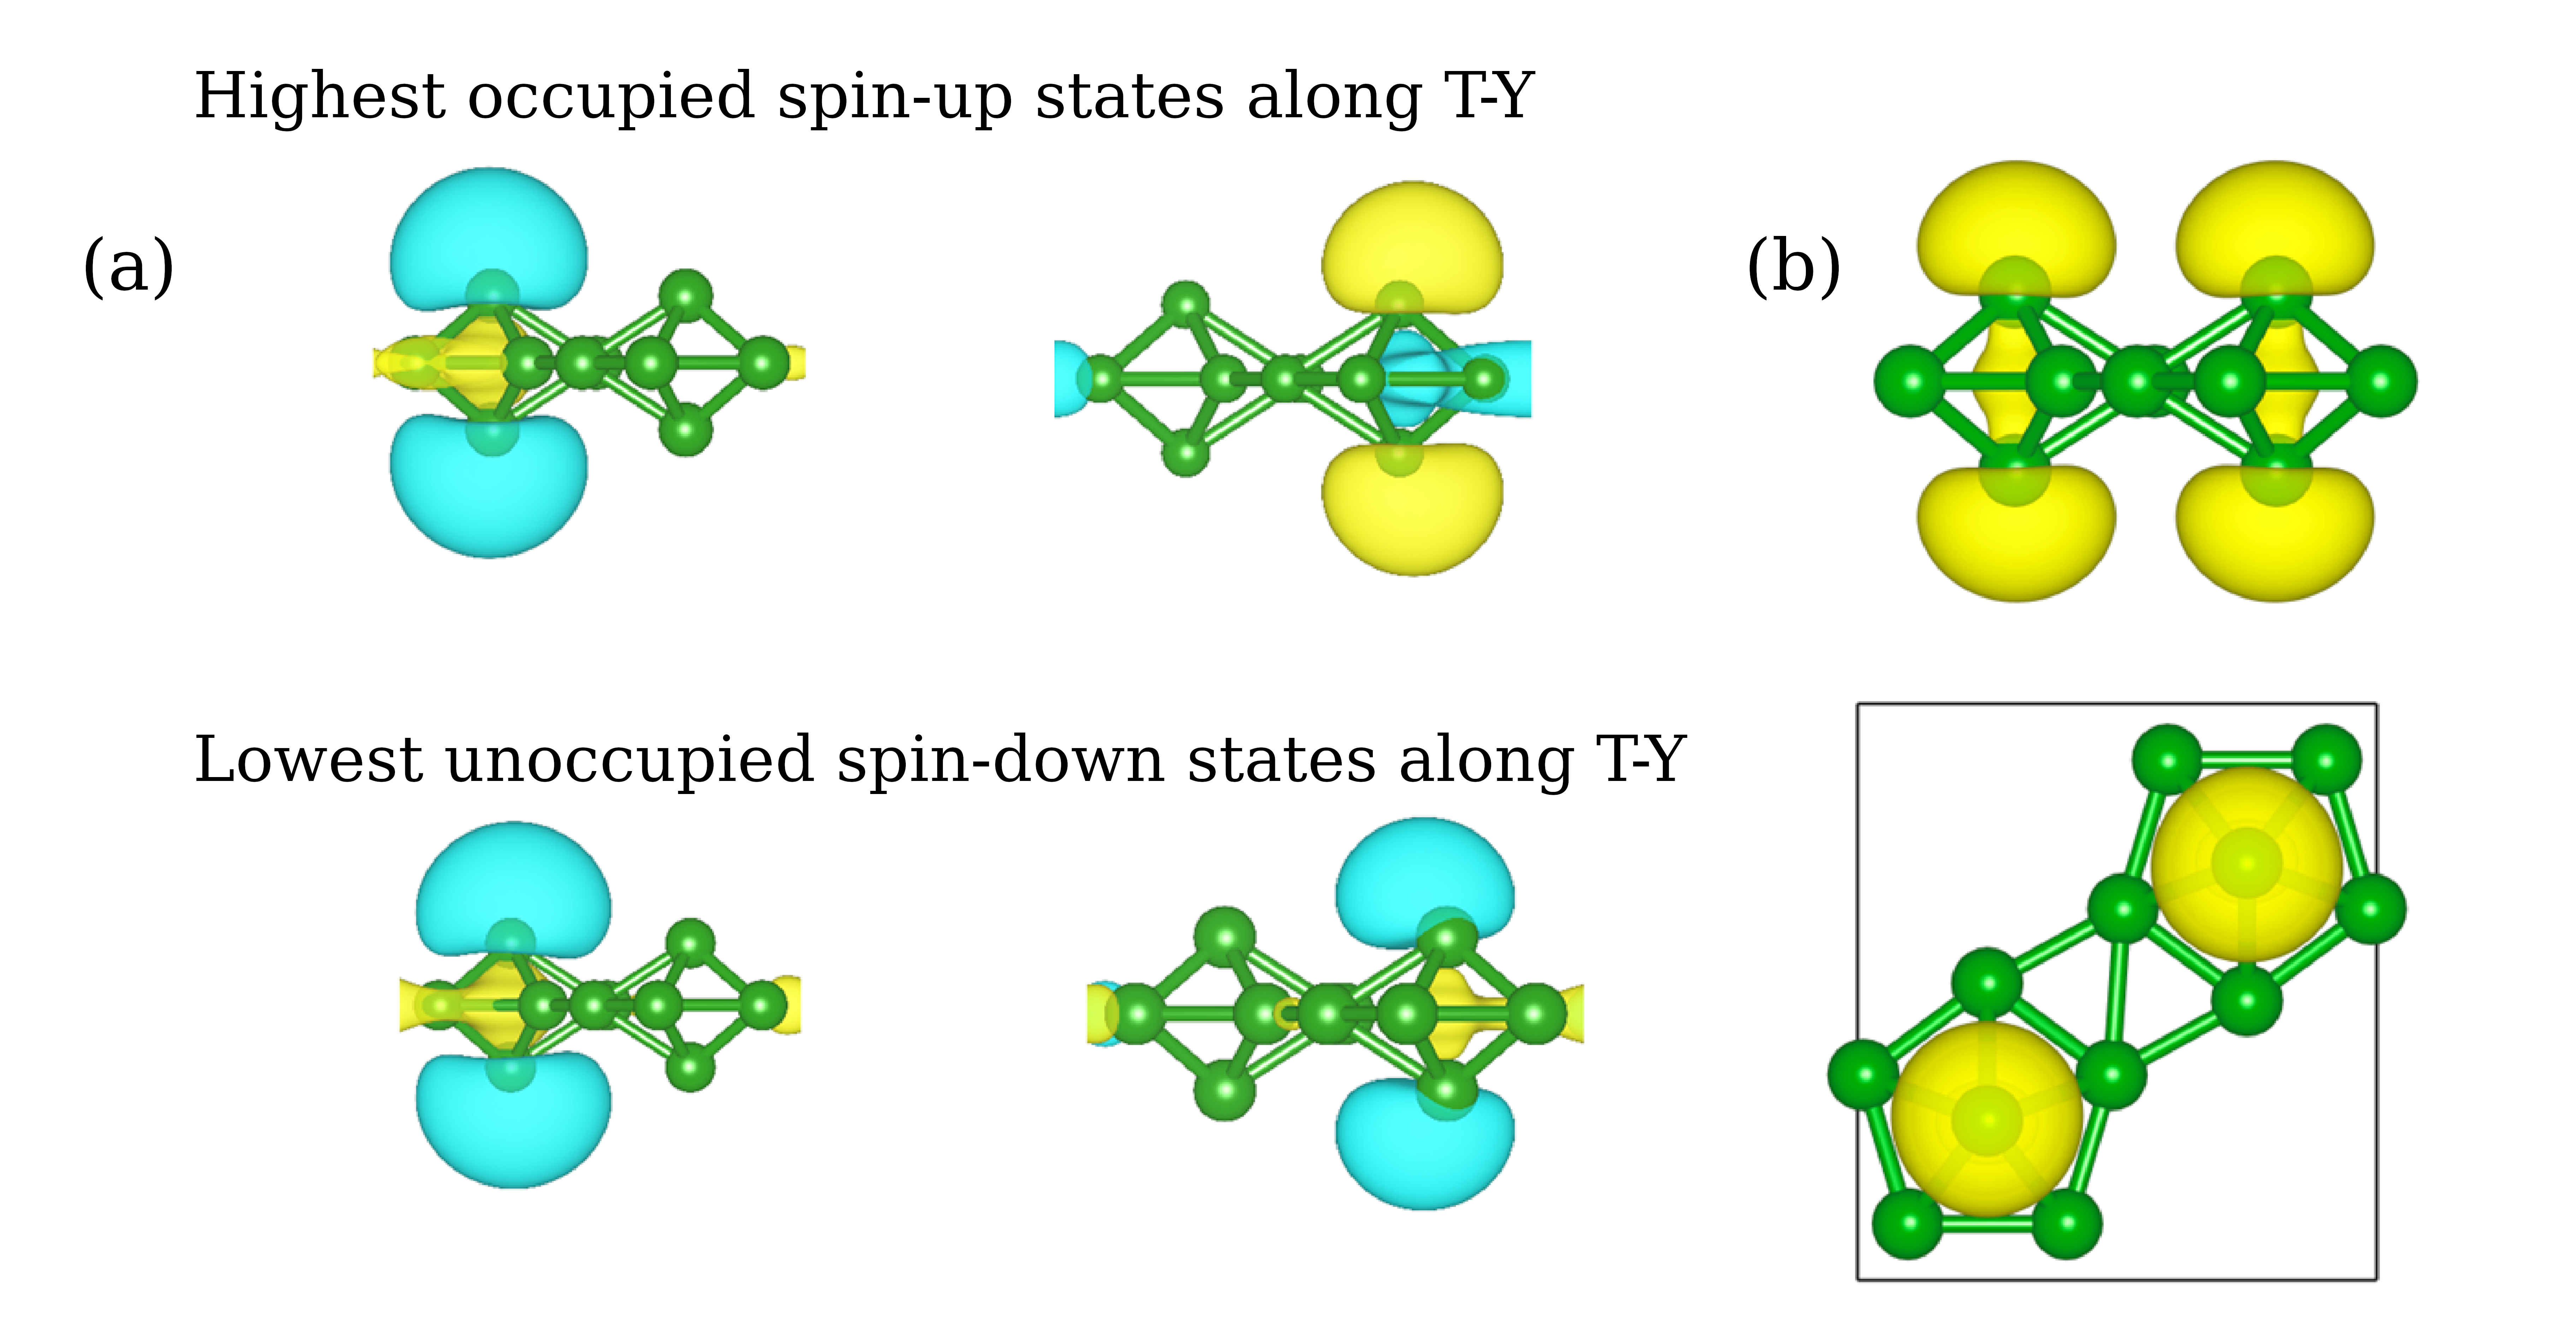
\includegraphics[width=0.80\textwidth]{figures_proj2/S2.17/S2.17.png}
\caption{(a) Highest occupied spin-up state and lowest unoccupied spin-down state of the FM monolayer,
taken midway along the high-symmetry $\mathrm{T}$--$\mathrm{Y}$ direction in the Brillouin zone.
(b) Corresponding spin density,
with an isosurface value of \qty{0.005}{e\per\angstrom\cubed}.}
\label{S2.17}
\end{figure}

\begin{figure}[!htbp]
\centering
    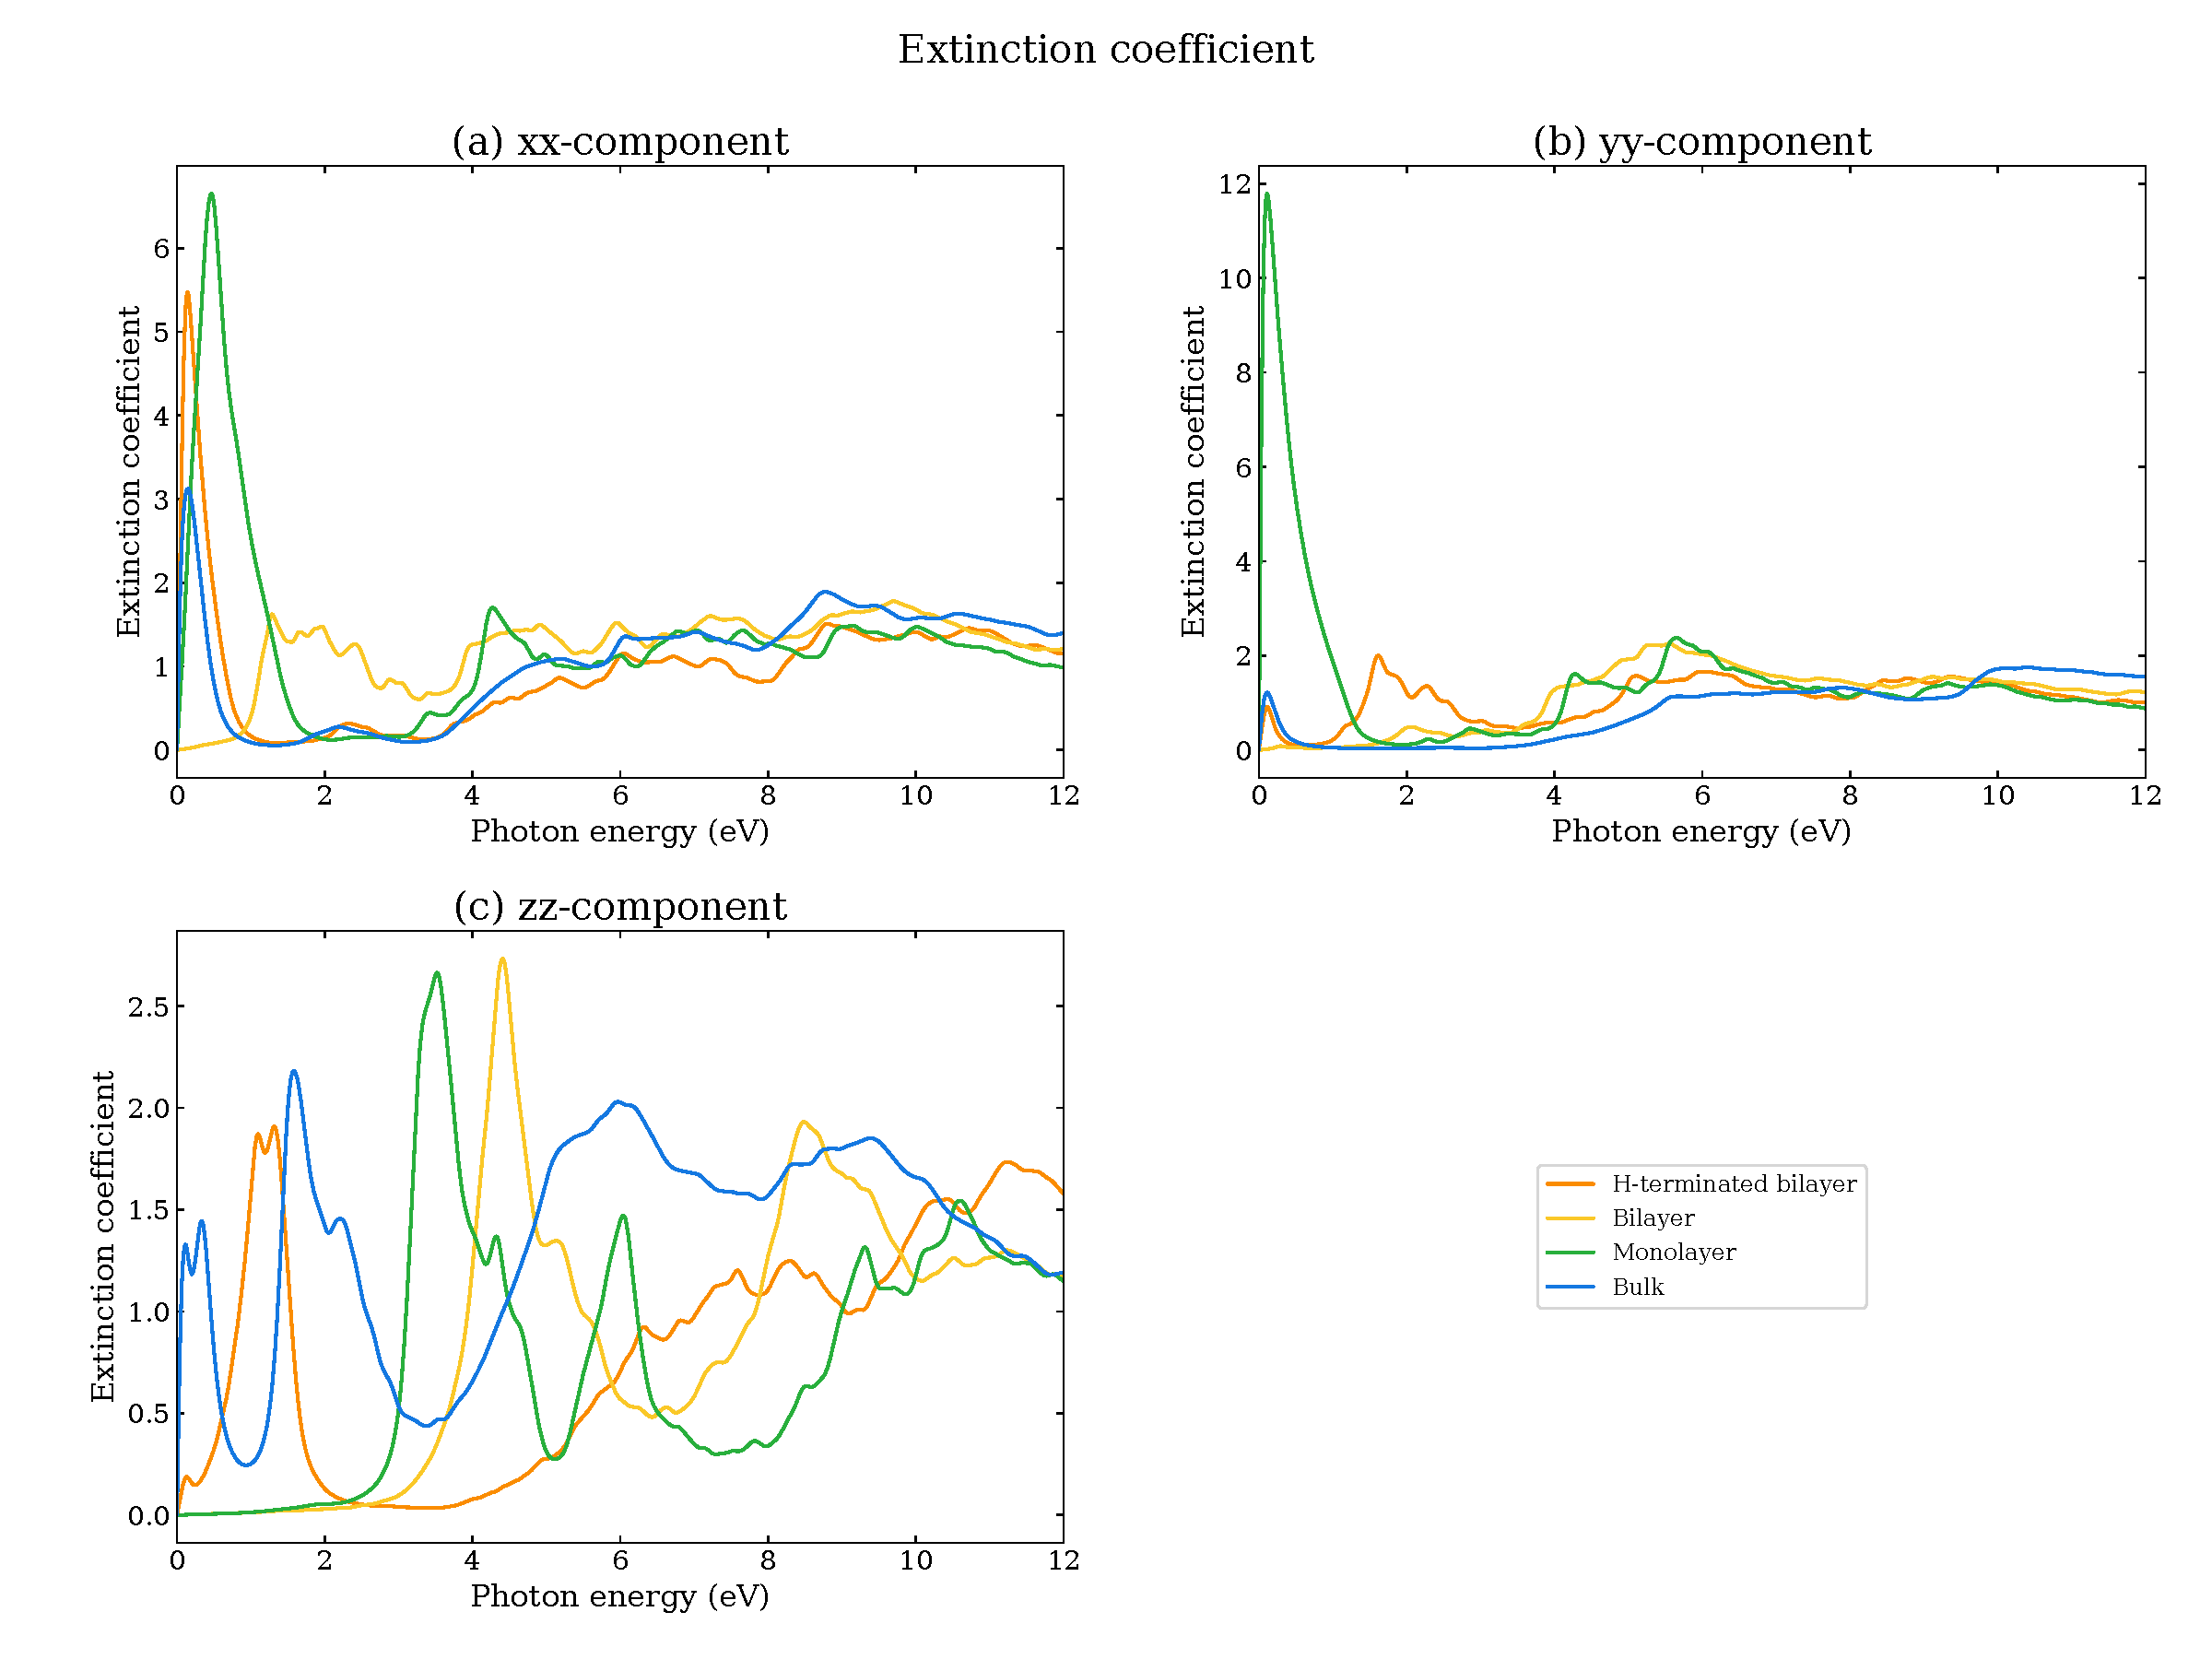
\includegraphics[width=0.80\textwidth]{figures_proj2/S2.18.pdf}
\caption{
Extinction coefficient as a function of energy for the o-\ce{B14} structures along the $xx$, $yy$, and $zz$ directions.
}
\label{S2.18}
\end{figure}

\cleardoublepage
\chapter[Properties of Pristine and Hydrogenated Beryllene]{Emergent Topological and Optical Properties in\\ Pristine and Hydrogen-Functionalized\\ Two-Dimensional Beryllium Phases}
\label{cha:project_beryllene}

This chapter is based on the manuscript by L.~Niu, O.~J.~Conquest, H.~Ma, C.~Verdi, and C.~Stampfl~\cite{niu2026draftemergent}.
The candidate carried out the \texttt{VASP} and postprocessing calculations, data analysis, and visualization.
Catherine Stampfl supervised the project.
Oliver James Conquest provided detailed guidance on the calculations.
Hongyang Ma performed the \texttt{Quantum ESPRESSO} and \texttt{EPW} calculations.
Carla Verdi performed the validation.
All authors contributed to writing or revising the manuscript.

\section{Abstract}
\label{3_abstract}

Two-dimensional elemental materials provide a direct platform for exploring electronic,
optical,
and topological phenomena arising from reduced dimensionality and modified bonding environments.
In this chapter,
we use density functional theory calculations to investigate the structural stability,
electronic structure,
optical response,
topological characteristics,
and superconductivity of pristine and hydrogen-functionalized beryllene systems.
The structures considered include monolayer $\alpha$-beryllene,
bilayer $\beta$-beryllene,
bulk reference phases,
and newly identified trilayer cubic beryllene,
an ABA-stacked trilayer beryllene with a square lattice.
In addition to confirming the stability of the previously proposed $\alpha$- and $\beta$-beryllene phases,
we predict a dynamically stable trilayer cubic beryllene phase with distinct electronic and optical characteristics.
Hydrogen functionalization drives $\alpha$-beryllene into a wide-gap semiconducting state with an HSE06 band gap of \qty{6.00}{\electronvolt},
whereas the hydrogen-functionalized $\beta$-beryllene structures remain metallic.
Only hydrogen-functionalized $\alpha$-beryllene is thermodynamically stable against \ce{H2} release under ambient conditions.
The calculated dielectric response reveals strong anisotropy and low-dimensional optical effects,
including a direction-dependent redistribution of visible-to-ultraviolet optical response
and distinct dielectric and energy-loss features.
Furthermore,
parity analysis of the spin-orbit-coupled electronic states shows that,
beyond $\alpha$-beryllene,
trilayer cubic beryllene has a conditional non-trivial $\mathbb{Z}_2$ index for its lowest six bands,
whereas all hydrogen-functionalized structures are trivial.
These six bands are isolated only by spin-orbit gaps of approximately \qty{1}{\milli\electronvolt} above the Fermi level.
Electron-phonon calculations predict phonon-mediated superconductivity in trilayer cubic beryllene and the hydrogen-functionalized $\beta$-beryllene structures,
with the highest anisotropic Migdal--Eliashberg transition temperature of approximately \qty{31.7}{\kelvin} in double-sided hydrogen-terminated $\beta$-beryllene.
These results identify beryllene as an elemental two-dimensional platform that combines metallicity,
tunable optical properties,
band inversions in selected subspaces,
and phonon-mediated superconductivity.

\section{Introduction}
\label{3_introduction}

Two-dimensional materials have reshaped modern materials science by enabling access to electronic,
thermal,
and mechanical properties that differ substantially from those of their bulk counterparts.
Since the isolation of graphene,
reduced dimensionality has been shown to give rise to Dirac fermions,
enhanced carrier mobility,
strong many-body interactions,
tunable band structures,
and anomalous phonon transport~\cite{novoselov2004electric,geim2007rise}.
These effects support rapid progress in nanoelectronics,
optoelectronics,
sensing,
thermal management,
and quantum technologies.

Beyond graphene,
the discovery and prediction of atomically thin materials have expanded to include transition-metal dichalcogenides,
hexagonal boron nitride,
black phosphorus,
and elemental two-dimensional materials,
commonly referred to as Xenes~\cite{butler2013progress,molle2018silicene}.
Elemental two-dimensional materials allow intrinsic structure-property relationships to be studied directly without the complexity introduced by multicomponent bonding.
However,
most experimentally realized Xenes are composed of relatively heavy elements,
where strong spin-orbit coupling,
substrate effects,
or structural buckling dominate the physics and may obscure low-energy electronic behaviour.

In contrast,
beryllium represents an extreme and largely unexplored limit within the family of elemental two-dimensional materials.
As the lightest alkaline-earth metal,
bulk beryllium combines low density,
high elastic modulus,
high thermal conductivity,
and transparency to X-rays and neutrons.
These properties have led to its use in aerospace,
nuclear,
and optical applications~\cite{zheng2020progress}.
Extending elemental beryllium into the two-dimensional limit raises the prospect of ultralight metallic layers with unconventional electronic and thermal properties governed by reduced dimensionality and strong confinement.

First-principles studies predicted that atomically thin beryllium could exist in metastable hexagonal or stable two-layer hexagonal lattice configurations~\cite{ono2020dynamical,hess2022periodicity}.
However,
for many years,
two-dimensional beryllium remained a theoretical construct due to experimental challenges associated with synthesis and handling.
This situation changed recently with the experimental realization of two-dimensional beryllium,
termed beryllene.
Chahal et al. reported the first experimental synthesis and characterization of beryllene using a sonochemical exfoliation approach starting from elemental beryllium powder~\cite{chahal2023beryllene}.
High-resolution transmission electron microscopy revealed atomically thin sheets with multiple structural motifs,
including hexagonal and square-like lattice geometries.
Raman spectroscopy and electron diffraction confirmed crystallinity,
while electrical measurements demonstrated intrinsic metallic conductivity.

Subsequent theoretical investigations have examined thermal transport in hexagonal monolayer beryllene.
Using first-principles phonon calculations combined with the Boltzmann transport equation,
Chowdhury and Mogurampelly predicted an in-plane lattice thermal conductivity of approximately \qty{270}{\watt\per\metre\per\kelvin} at room temperature,
which exceeds that of bulk beryllium~\cite{chowdhury2024unusual}.
This enhancement was attributed to suppressed phonon-phonon scattering and the dominant contribution of long-wavelength flexural phonons,
a feature rarely observed in atomically thin metallic systems.
These results suggest that two-dimensional beryllium could serve as an efficient heat-spreading material in nanoscale electronic architectures.

Beyond thermal properties,
the electronic structure of beryllene has been predicted to host non-trivial quantum features.
Several density functional theory studies have identified Dirac-like band crossings near the Fermi level in hexagonal monolayer and bilayer beryllene,
usually denoted as $\alpha$- and $\beta$-beryllene,
arising from symmetry-protected $s$-$p$ orbital hybridization~\cite{li2023coexistence}.
Electron-phonon coupling calculations further predict phonon-mediated superconductivity in these phases,
with transition temperatures on the order of \qty{10}{\kelvin}.
The coexistence of Dirac fermions and superconductivity in an ultralight elemental monolayer distinguishes beryllene from both graphene and heavier Xenes.

The possibility of topological behaviour in two-dimensional beryllium has also been explored from a more fundamental perspective.
Derriche et al. demonstrated that light-element lattices dominated by charge-based interactions can host topologically protected electronic states even in the absence of strong spin-orbit coupling~\cite{derriche2024light}.
These findings suggest that beryllene may realize topological phases driven mainly by lattice symmetry and orbital physics,
offering an alternative route to low-dissipation electronic states without relying on heavy elements.
While experimental studies of beryllene remain limited,
earlier work on ultrathin beryllium films and nanostructures has revealed unconventional quantum transport behaviour,
including strong disorder effects and superconducting correlations at low temperatures~\cite{xiong2009spin}.

Two-dimensional topological materials are candidates for quantum and electronic technologies because their non-trivial band topology gives rise to symmetry-protected edge states that resist disorder and backscattering~\cite{weber2024roadmap}.
Recent density functional theory studies have shown that simple elemental two-dimensional systems can host switchable or adsorbate-induced topological behaviour.
For example,
interlayer sliding in bilayer elemental bismuth was predicted to switch the system between topologically trivial and non-trivial phases~\cite{qian2025switchable}.
Similarly,
hydrogenation and strain can tune monolayer arsenene into a quantum spin Hall state with a sizable band gap~\cite{zhang2016controllable}.
These studies indicate that structural control and adsorbate functionalization can provide practical routes to topological phases in elemental two-dimensional materials.

Although two-dimensional elemental beryllium has recently been realized experimentally and shown to exhibit unusual electronic and thermal properties,
its interaction with hydrogen has received much less attention.
First-principles investigations of hydrogen adsorption on low-index hexagonal close-packed beryllium surfaces,
particularly Be(0001),
show that hydrogen binds preferentially to high-symmetry adsorption sites with moderate binding energies and induces appreciable local lattice relaxation~\cite{bachurin2015ab}.
These results indicate that beryllium-hydrogen interactions occupy an intermediate regime between weak physisorption and strong ionic hydride formation.
In the two-dimensional limit,
reduced coordination and enhanced lattice flexibility are expected to modify this balance,
potentially stabilizing adsorption geometries or electronic reconstructions that are inaccessible on bulk surfaces.
Global structure search and density functional theory calculations predicted two stable beryllium hydride monolayers with multicentre beryllium-hydrogen bonding motifs and wide band gaps~\cite{li2018global}.
Although such systems correspond to compound formation rather than surface termination,
they demonstrate that hydrogen can strongly reshape bonding and electronic behaviour in low-dimensional beryllium-based systems.

In this chapter,
we use density functional theory calculations to investigate the atomic,
electronic,
optical,
topological,
and superconducting properties of pristine and hydrogen-functionalized beryllene systems.
In addition to $\alpha$- and $\beta$-beryllene,
the pristine structures include trilayer cubic beryllene,
by which we denote ABA-stacked trilayer beryllene with a square lattice.
The hydrogen-functionalized structures are double-sided hydrogen-terminated $\alpha$-beryllene (2H-$\alpha$-beryllene)
and single-sided and double-sided hydrogen-terminated $\beta$-beryllene (1H-$\beta$-beryllene and 2H-$\beta$-beryllene).
The results identify dynamically stable 2H-$\alpha$-beryllene and a trilayer cubic beryllene phase with a conditional non-trivial $\mathbb{Z}_2$ index for an isolated band subspace.
Electron-phonon calculations further predict phonon-mediated superconductivity in trilayer cubic beryllene, 1H-$\beta$-beryllene, and 2H-$\beta$-beryllene.
The optical properties demonstrate direction-dependent and dimensionality-dependent response,
together with anisotropic dielectric and energy-loss spectra and a redistribution of visible-to-ultraviolet optical response.

\section{Computation methods}
\label{3_methods}

The density functional theory calculations are performed using the Vienna Ab initio Simulation Package,
\texttt{VASP}~\cite{kresse1993ab,kresse1994ab,kresse1996efficiency,kresse1996efficient}.
We use the projector augmented wave method to describe the electron-ion interactions~\cite{kresse1999ultrasoft}.
The generalized gradient approximation of Perdew--Burke--Ernzerhof is employed for the exchange-correlation functional~\cite{perdew1996generalized}.
The structural relaxations,
total energies,
phonon calculations,
and molecular dynamics simulations are performed without a dispersion correction.
We include the D3 dispersion correction with Becke--Johnson damping~\cite{becke2005density,grimme2010consistent,grimme2011effect} in the PBE band-structure calculations without spin-orbit coupling.
At the fixed relaxed geometries,
this correction adds only an energy term and leaves the Kohn--Sham eigenvalues unchanged.
The PBE band structures are calculated non-self-consistently from the self-consistent charge densities,
and their energies are given relative to the Fermi level of the corresponding self-consistent calculations.

For bulk hexagonal close-packed (hcp) beryllium and bulk body-centred cubic (bcc) beryllium,
a $\Gamma$-centred k-point mesh of $27 \times 27 \times 27$ is used for the total energies and structural relaxations.
A $105 \times 105 \times 105$ mesh is used for the calculation of the complex dielectric function.
We use a plane-wave cutoff of \qty{600}{\electronvolt} for all calculations except the molecular dynamics simulations described below.
The electronic convergence criterion is set to \qty{1e-6}{\electronvolt},
and the structures are relaxed until all forces on each atom are below \qty{0.001}{\electronvolt\per\angstrom}.
For the two-dimensional structures,
the full supercell height normal to the layers is \qty{40}{\angstrom}, including the slab and the surrounding vacuum,
and a dipole correction is applied along the surface normal~\cite{neugebauer1992adsorbate}.
We relax the in-plane lattice vectors and the atomic positions with this supercell height fixed.
A k-point mesh of $27 \times 27 \times 1$ is used for the hexagonal structures,
whereas a $25 \times 25 \times 1$ mesh is used for the cubic structures.
For all two-dimensional systems,
we calculate the complex dielectric function on a $105 \times 105 \times 1$ mesh.
Convergence tests for the cohesive and total energies,
as well as for the dielectric function with respect to the k-point mesh and the number of bands included through \texttt{NBANDS},
are shown in figures~\ref{fig:proj3_cohesive_energy_convergence}--\ref{fig:proj3_cubic_dielectric_kpoint_convergence} in section~\ref{3_supplementary}.
With the selected meshes,
the cohesive energies of bulk hcp beryllium,
$\alpha$-beryllene,
bulk bcc beryllium,
and trilayer cubic beryllene lie within \qty{0.3}{\milli\electronvolt} per atom of the values for the densest meshes tested.
These densest meshes are $41 \times 41 \times 41$ for the bulk phases and $47 \times 47 \times 1$ for the two-dimensional structures.
Over all denser meshes,
the cohesive energies stay within \qty{2.2}{\milli\electronvolt} per atom of the values for the selected meshes.

The dynamical stability of the structures is examined using finite-displacement phonon calculations with \texttt{phonopy}~\cite{togo2015first,togo2023implementation},
with atomic displacements of \qty{0.01}{\angstrom}.
We use $5 \times 5 \times 1$ supercells for the two-dimensional structures,
except for trilayer cubic beryllene,
for which a $4 \times 4 \times 1$ supercell is used.
The supercells of bulk hcp and bulk bcc beryllium are $4 \times 4 \times 3$ and $4 \times 4 \times 4$,
respectively.
The forces are calculated with Gaussian smearing of \qty{0.05}{\electronvolt},
an electronic convergence criterion of \qty{1e-8}{\electronvolt},
and supercell k-point meshes equivalent to approximately $65 \times 65$ per unit cell for the metallic two-dimensional structures.
The relaxed cells of $\alpha$-beryllene and 2H-$\alpha$-beryllene deviate from hexagonal symmetry by up to \qty{1e-4}{\angstrom}.
For these structures,
we determine the symmetry with a tolerance of \qty{1e-3}{\angstrom}.
A tighter tolerance gives a lower-symmetry space group and breaks the equivalence of the supercell images in the interpolation.
The soft mode of 2H-$\beta$-beryllene is further examined with the frozen-phonon calculations described in section~\ref{3_supplementary}.
The preliminary phonon calculations,
which are not discussed further,
include the D3 dispersion correction.
The finite-temperature stability of the hydrogen-functionalized structures is examined using \textit{ab initio} molecular dynamics simulations.
These simulations use $5 \times 5 \times 1$ supercells without the dipole correction,
with supercell heights of \qty{26.7}{\angstrom} for 2H-$\alpha$-beryllene and \qty{40}{\angstrom} for 1H-$\beta$-beryllene and 2H-$\beta$-beryllene.
We use a Nos\'e--Hoover thermostat at \qty{300}{\kelvin}~\cite{nose1984unified,hoover1985canonical},
a time step of \qty{0.5}{\femto\second},
a total simulation time of \qty{5.5}{\pico\second},
a plane-wave cutoff of \qty{350}{\electronvolt},
and a $3 \times 3 \times 1$ k-point mesh.

The adsorption energy per hydrogen atom,
$E_{\mathrm{ad}}$,
is calculated as:

\begin{equation}
    E_{\mathrm{ad}} =
    \frac{E_{\mathrm{H/Be}}-E_{\mathrm{Be}}-n_{\mathrm{H}}E_{\mathrm{H}}}{n_{\mathrm{H}}}
\label{eq:proj3_hydrogen_adsorption_energy}
\end{equation}

here,
$E_{\mathrm{H/Be}}$ is the total energy of the hydrogen-functionalized system,
$E_{\mathrm{Be}}$ is the total energy of the corresponding pristine two-dimensional beryllium structure,
$E_{\mathrm{H}}$ is the energy per hydrogen atom in an isolated \ce{H2} molecule,
and $n_{\mathrm{H}}$ is the number of hydrogen atoms in the unit cell.
A negative value indicates that hydrogen adsorption is exothermic.
To include vibrational contributions,
we add the harmonic zero-point energies of the hydrogen-functionalized and pristine structures,
obtained from the phonon calculations on a $40 \times 40$ q-point mesh with imaginary modes excluded.
We also add the zero-point energy of \ce{H2},
\qty{0.269}{\electronvolt},
obtained from its calculated stretching frequency of \qty{4341}{\per\centi\metre}.
The adsorption free energy at \qty{298.15}{\kelvin} and \qty{1}{\bar} further includes the harmonic vibrational free energies of the beryllene layers,
and the enthalpy and entropy of gaseous \ce{H2} from the NIST-JANAF tables~\cite{chase1998nist}.

The cohesive energy per atom,
$E_{\mathrm{c}}$,
of the beryllium systems is calculated as:

\begin{equation}
    E_{\mathrm{c}} =
    \frac{E_{\mathrm{Be\text{-}struc}}-n_{\mathrm{Be}}E_{\mathrm{Be\text{-}atom}}}{n_{\mathrm{Be}}}
\label{eq:proj3_cohesive_energy}
\end{equation}

here,
$E_{\mathrm{Be\text{-}struc}}$ is the total energy of the beryllium structure of interest,
$E_{\mathrm{Be\text{-}atom}}$ is the total energy of a free beryllium atom calculated in a large supercell,
and $n_{\mathrm{Be}}$ is the number of beryllium atoms in the unit cell.

For the topological calculations,
we use a plane-wave cutoff of \qty{600}{\electronvolt},
a $105 \times 105 \times 1$ k-point mesh,
and the same supercell height of \qty{40}{\angstrom} with the dipole correction.
The electronic convergence criterion is set to \qty{1e-8}{\electronvolt},
and Gaussian smearing of \qty{0.01}{\electronvolt} is used.
Spin-orbit coupling is included in the band-structure and parity calculations.
We calculate the parity eigenvalues of the spinor wave functions using \texttt{IrRep}~\cite{iraola2022irrep},
and check them independently with the inversion matrix reconstructed from the wave functions in double precision.
For a time-reversal invariant momentum $\vec{\Lambda}_i$,
the parity product of the lowest $N$ spinor bands is given by:

\begin{equation}
    \delta_i =
    \prod_{m=1}^{N/2}
    \xi_{2m}(\vec{\Lambda}_i\,)
\label{eq:proj3_parity_product}
\end{equation}

here,
$\xi_{2m}(\vec{\Lambda}_i\,)=\pm1$ is the parity eigenvalue of one state in the $m$th Kramers pair at $\vec{\Lambda}_i$,
and $N$ is the number of spinor bands in the selected subspace.
Thus, $N=2N_\mathrm{p}$ in the notation of chapter~\ref{cha:fundamentals_c}.
The $\mathbb{Z}_2$ index is then obtained from the Fu--Kane product over the four time-reversal invariant momenta of the two-dimensional Brillouin zone,
$\Gamma=(0,0)$,
$\mathrm{X}=(1/2,0)$,
$\mathrm{Y}=(0,1/2)$,
and $\mathrm{M}=(1/2,1/2)$ in units of the reciprocal lattice vectors~\cite{fu2007topological,fu2007topological3d}:

\begin{equation}
    (-1)^{\nu} =
    \prod_{i=1}^{4} \delta_i
\label{eq:proj3_z2_index}
\end{equation}

here,
$\nu=1$ denotes non-trivial topology,
whereas $\nu=0$ denotes trivial topology.
The derivation of this criterion and its application to an isolated band subspace are discussed in sections~\ref{sec:fu_kane_criterion_topology} and~\ref{sec:interpreting_topology_calculation}.
For 1H-$\beta$-beryllene,
which has no inversion symmetry,
$\nu$ is obtained from the evolution of the Wannier charge centres on 23 Wilson loops across half of the Brillouin zone~\cite{soluyanov2011computing,gresch2017z2pack}.
We calculate the Wannier charge centres with \texttt{Z2Pack} from the overlaps of the spin-orbit-coupled wave functions,
written through the interface between \texttt{VASP} and \texttt{Wannier90}~\cite{pizzi2020wannier90}.
The Wilson loops are refined until the convergence checks of \texttt{Z2Pack} are passed.
For the metallic structures,
the lowest $N$ bands are not completely filled.
We therefore check the isolation of this subspace with the direct gap $E_{N+1}(\vec{k}\,)-E_{N}(\vec{k}\,)$ on the $105 \times 105$ mesh,
along the band paths,
and on locally refined meshes around each minimum.
The time-reversal symmetry assumed in this analysis is checked with spin-polarized calculations started from ferromagnetic and antiferromagnetic configurations.

To test the band gap and the band order beyond the semilocal approximation,
we also use the HSE06 hybrid functional~\cite{heyd2003hybrid,krukau2006influence} without spin-orbit coupling.
These calculations use a supercell height of \qty{20}{\angstrom},
a $\Gamma$-centred $12 \times 12 \times 1$ k-point mesh,
and the same q-point mesh for the Fock exchange.
Inversion acts only on the spatial part of the wave functions,
and the spin-orbit splittings of Be and H are approximately \qty{1}{\milli\electronvolt}.
We therefore compare the parities of the spinless states at the time-reversal invariant momenta directly with those of the Kramers pairs.
The HSE06 band structure of 2H-$\alpha$-beryllene is calculated at 71 points along the $\Gamma$--$\mathrm{K}$--$\mathrm{M}$--$\Gamma$ path and at 9 points around each PBE band edge.

The \texttt{Quantum ESPRESSO} calculations~\cite{giannozzi2017advanced,giannozzi2009quantum} are performed on the structures relaxed with the PBE functional,
except for the phonon and electron-phonon calculations of 2H-$\beta$-beryllene described below.
We use optimized norm-conserving Vanderbilt pseudopotentials~\cite{hamann2013optimized},
where the Be $1s$ states are considered to be valence states.
The plane-wave cutoffs are \qty{80}{Ry} and \qty{640}{Ry} for the wave functions and charge density, respectively,
and the Marzari--Vanderbilt smearing is \qty{0.02}{Ry}~\cite{marzari1999thermal}.
We also use a two-dimensional Coulomb cutoff~\cite{sohier2017density},
along with a vacuum of about \qty{15}{\angstrom} or larger.
The k-point meshes of the self-consistent calculations are $56 \times 56 \times 1$,
$52 \times 52 \times 1$, $46 \times 46 \times 1$,
and $52 \times 57 \times 1$ for trilayer cubic beryllene,
2H-$\alpha$-beryllene,
2H-$\beta$-beryllene,
and 1H-$\beta$-beryllene,
respectively.
The relaxed structures are listed in table~\ref{tab:proj3_qe_structures} in section~\ref{3_supplementary}.
To examine the band topology of these structures,
we recalculate the parities at the time-reversal invariant momenta with fully relativistic projector augmented wave pseudopotentials~\cite{dalcorso2014pseudopotentials},
with plane-wave cutoffs of \qty{90}{Ry} and \qty{720}{Ry},
and with spin-orbit coupling.
We also compute Wilson loops~\cite{yu2011equivalent} with \texttt{WannierTools}~\cite{wu2018wanniertools},
based on Wannier function models generated with \texttt{Wannier90}~\cite{pizzi2020wannier90}.

Phonons of trilayer cubic beryllene,
2H-$\beta$-beryllene,
and 1H-$\beta$-beryllene are computed using density functional perturbation theory~\cite{baroni2001phonons} on a $12 \times 12 \times 1$ q-point mesh,
and electron-phonon coupling is calculated using \texttt{EPW}~\cite{lee2023electron,giustino2007electron}.
For 2H-$\beta$-beryllene,
these calculations use a structure relaxed with the D3 dispersion correction with Becke--Johnson damping,
with a lattice constant of \qty{2.53}{\angstrom},
and include this correction.
The Wannier functions are initialized with projections on the Be $s$ and $p$ orbitals and the H $s$ orbitals,
and the Be $1s$ bands are excluded.
Electronic states and phonon perturbations are Wannier-interpolated from coarse $24 \times 24 \times 1$ k-point and $12 \times 12 \times 1$ q-point meshes to $80 \times 80 \times 1$ fine meshes,
and the convergence is checked using $40 \times 40 \times 1$ fine meshes.
Electronic and phonon smearings are set to \qty{0.15}{\electronvolt} and \qty{0.5}{\milli\electronvolt}, respectively,
and the Matsubara-frequency cutoff is \qty{1.2}{\electronvolt}.
Electronic states within \qty{0.6}{\electronvolt} of the Fermi level are included.
Phonon modes below \qty{40}{\per\centi\metre}, approximately \qty{5}{\milli\electronvolt},
are excluded from the electron-phonon coupling of trilayer cubic beryllene and 2H-$\beta$-beryllene.
This threshold follows from convergence tests.
Above it, $\lambda$ changes little with the fine meshes and the other calculation settings,
whereas the contribution below it comes from acoustic modes near $\Gamma$ and does not converge.
We therefore treat this contribution as a numerical artefact.
For 1H-$\beta$-beryllene,
the modes below \qty{40}{\per\centi\metre} contribute less than \qty{1}{\percent} of $\lambda$,
and only the modes below \qty{5}{\per\centi\metre} are excluded.
The effect of this threshold is given in table~\ref{tab:proj3_epw_threshold} and figure~\ref{fig:proj3_a2f} in section~\ref{3_supplementary}.
The electron-phonon coupling strength $\lambda$ and the logarithmic average frequency $\omega_\mathrm{log}$ are extracted from the Eliashberg spectral function $\alpha^2F(\omega)$ through equations~\eqref{eliashberg_spectral_function_method} and~\eqref{electron_phonon_spectral_moments}.
The superconducting transition temperature $T_\mathrm{c}$ is calculated in two ways.
Firstly, the simplified Allen--Dynes expression in equation~\eqref{allen_dynes_temperature_estimate}~\cite{allen-dynes,mcmillan1968transition} is used with the Coulomb pseudopotential $\mu^*$ varying from 0.10 to 0.16.
Secondly, the isotropic Migdal--Eliashberg equations on the imaginary axis~\cite{giustino2017electron,eliashberg1960interactions,migdal1958interaction} are solved with $\mu^*=0.13$,
and the isotropic $T_\mathrm{c}$ is found by fitting the temperature dependence of the gap at the first Matsubara frequency.
For 2H-$\beta$-beryllene and 1H-$\beta$-beryllene,
the anisotropic Migdal--Eliashberg equations~\cite{margine2013anisotropic} are also solved for each temperature using up to 6000 iterations.
Close to $T_\mathrm{c}$, the convergence is very slow.
Therefore, the gap is monitored throughout the iterations.
A temperature is considered below $T_\mathrm{c}$ if the extrapolated gap converges to a non-zero value for all fitted ranges,
and above $T_\mathrm{c}$ if the gap exponentially decreases with increasing number of iterations.
Finally, $T_\mathrm{c}$ is estimated from the extrapolation of the limiting gaps below $T_\mathrm{c}$ and the decay rates above $T_\mathrm{c}$.

For the optical calculations,
we calculate the frequency-dependent dielectric tensor $\varepsilon_{\alpha\beta}(\omega)$ within \texttt{VASP}.
The microscopic expression for the dielectric response,
the Kramers--Kronig relation,
and the derived optical quantities are introduced in chapter~\ref{cha:fundamentals_b},
especially sections~\ref{sec:from_electronic_response_to_dielectric_function} and~\ref{sec:from_dielectric_function_to_optical_properties}.
Therefore, we do not repeat these formula definitions here.
In this chapter,
we apply these scalar definitions separately to the Cartesian diagonal components $\varepsilon_{\lambda\lambda}(\omega)$,
with $\lambda=x,y,z$.
They give the usual principal-component optical quantities when the dielectric tensor is diagonal in the chosen coordinates and the propagation geometry is compatible with that component.
The off-diagonal coupling in monoclinic 1H-$\beta$-beryllene and 2H-$\beta$-beryllene is not included in the derived spectra,
which therefore provide scalar comparisons.
In particular,
$L_{\lambda}(\omega)$ uses the inverse of $\varepsilon_{\lambda\lambda}(\omega)$,
which can differ from the corresponding component of the inverse tensor.
The reflectivity describes a homogeneous semi-infinite medium in the scalar normal-incidence approximation.

For all eight selected optical datasets,
we use the independent-particle approximation in \texttt{VASP} 6.5.0 with \texttt{LOPTICS=T}.
These calculations are spin-unpolarized and do not include spin-orbit coupling
(\texttt{ISPIN=1} and \texttt{LSORBIT=F}).
We use Gaussian occupation smearing of \qty{0.01}{\electronvolt}
(\texttt{ISMEAR=0} and \texttt{SIGMA=0.01})
and a complex frequency shift of \qty{0.1}{\electronvolt} (\texttt{CSHIFT=0.1}).
The spectra include interband transitions without microscopic local-field effects or a Drude contribution
(\texttt{WPLASMAI=0}),
and the postprocessing adds no Drude term.
They therefore describe the interband part of the low-frequency response of these metallic systems.
For the two-dimensional systems,
the calculated dielectric tensor contains the combined dielectric response of the material and the vacuum region.
We therefore normalize the calculated dielectric functions with equation~\eqref{optical_volume_normalization_2d}
to obtain the effective dielectric response under the chosen thickness convention~\cite{yang2021method}.
The full normal supercell height for the two-dimensional optical calculations is \qty{40}{\angstrom}.
We assign the effective thickness $d_{\mathrm{2D}}$ as the separation of the outermost atomic centres along the surface normal,
plus the radii of the atoms at those two surfaces.
These radii are \qty{1.98}{\angstrom} for Be and \qty{0.70}{\angstrom} for H.
The same optical volume normalization is applied to the $xx$, $yy$, and $zz$ components,
and the absolute effective response depends on this thickness convention.
The effective thicknesses and the actual total numbers of bands are given in section~\ref{3_supplementary}.

\section{Results and discussion}
\label{3_results}

\subsection{Atomic structure}
\label{3_atomic_structure}

We first examine the atomic structures of the bulk reference phases,
pristine two-dimensional beryllium phases,
and hydrogen-functionalized beryllene structures considered in this chapter.
Figures~\ref{fig:proj3_bulk_structures}, \ref{fig:proj3_pristine_2d_structures}, and~\ref{fig:proj3_hydrogenated_structures} show the bulk reference structures,
the pristine two-dimensional structures,
and the hydrogen-functionalized structures,
respectively.

\begin{figure}[!htbp]
\centering
    
\includegraphics[width=1.00\linewidth]{figures_proj3/structure_bulk_thesis.pdf}
\caption{Atomic structures of the bulk beryllium phases.
Left and middle: top and side views of bulk hcp beryllium.
Right: bulk bcc beryllium, for which the top and side views are equivalent.
Beryllium atoms are shown in green,
and the unit cells are outlined.}
\label{fig:proj3_bulk_structures}
\end{figure}

Bulk beryllium is known experimentally to adopt the hexagonal close-packed structure under ambient conditions.
In contrast,
the body-centred cubic phase is stable only close to the melting point and has been predicted,
but not conclusively observed,
at high pressure.
We include this phase as a bulk reference structure.
The optimized lattice constants of bulk hcp beryllium, $a=\qty{2.266}{\angstrom}$ and $c=\qty{3.561}{\angstrom}$, are smaller than the values measured at room temperature by less than \qty{1}{\percent}~\cite{gordon1949high}.
The optimized cohesive energy of bulk hcp beryllium is \qty{-3.73}{\electronvolt} per atom,
which is \qty{0.10}{\electronvolt} per atom lower than that of bulk bcc beryllium.
These two bulk phases provide useful reference points for comparing the bonding geometry,
electronic structure,
and optical response of the low-dimensional beryllium systems discussed below.

\begin{figure}[!htbp]
\centering
    \includegraphics[width=1.00\linewidth]{figures_proj3/structure_pristine_thesis.pdf}
\caption{Atomic structures of the pristine two-dimensional beryllium phases.
Left: top and side views of $\alpha$-beryllene.
Middle: top and side views of $\beta$-beryllene.
Right: top and side views of trilayer cubic beryllene.
Beryllium atoms are shown in green,
except for the lower layer of $\beta$-beryllene and the central layer of trilayer cubic beryllene,
which are shown in cyan.
The unit cells are outlined.}
\label{fig:proj3_pristine_2d_structures}
\end{figure}

Among the pristine two-dimensional phases,
$\alpha$-beryllene and $\beta$-beryllene correspond to the previously proposed hexagonal monolayer and bilayer forms of beryllene.
$\alpha$-beryllene forms a planar hexagonal network,
where each beryllium atom bonds to six neighbouring beryllium atoms.
$\beta$-beryllene can be regarded as a bilayer form of $\alpha$-beryllene,
where beryllium atoms in the upper layer sit above hollow sites of the lower layer.
This buckled honeycomb structure has $P\bar{3}m1$ symmetry.
In addition to these known phases,
we also identify a trilayer cubic beryllene structure.
This structure is an ABA-stacked trilayer with a square lattice,
where the beryllium atoms in the central layer are located at the hollow sites of the upper and lower layers.
It therefore provides a distinct structural motif within the same elemental system.

The cohesive energies of $\alpha$-beryllene,
$\beta$-beryllene,
and trilayer cubic beryllene are \qty{0.79}{\electronvolt},
\qty{0.44}{\electronvolt},
and \qty{0.43}{\electronvolt} per atom less favourable than that of bulk hcp beryllium,
respectively.
Compared with bulk hcp beryllium,
the in-plane lattice constants of $\alpha$-beryllene and $\beta$-beryllene are reduced by \qty{6.1}{\percent} and \qty{4.4}{\percent},
respectively.
The interlayer beryllium-beryllium distance in $\beta$-beryllene is \qty{7.2}{\percent} larger than that in bulk hcp beryllium.
Trilayer cubic beryllene is constructed from three (001) layers of bulk bcc beryllium.
Relative to bulk bcc beryllium,
its in-plane lattice constant is \qty{12.7}{\percent} smaller than the cubic lattice constant,
but only \qty{0.8}{\percent} larger than the nearest-neighbour distance.
In contrast,
its interlayer distance is \qty{20.2}{\percent} larger than the spacing between the (001) layers.

We also test monolayer, bilayer, and quadlayer cubic beryllene structures,
as well as graphene-like beryllium layers from one to four layers.
These structures are dynamically unstable in preliminary phonon calculations
and are therefore not discussed further.

\begin{figure}[!htbp]
\centering
    \includegraphics[width=1.00\linewidth]{figures_proj3/structure_hydrogenated_thesis.pdf}
\caption{Atomic structures of the hydrogen-functionalized beryllene phases.
Left: double-sided hydrogen-terminated $\alpha$-beryllene (2H-$\alpha$-beryllene).
Middle: single-sided hydrogen-terminated $\beta$-beryllene (1H-$\beta$-beryllene).
Right: double-sided hydrogen-terminated $\beta$-beryllene (2H-$\beta$-beryllene).
Upper row: top views. Middle and lower rows: side views along the $x$ and $y$ axes, respectively.
Beryllium atoms are shown in green,
except for the lower layer of 1H-$\beta$-beryllene and 2H-$\beta$-beryllene,
which is shown in cyan.
Hydrogen atoms above and below the beryllium layers are shown in orange and light orange,
respectively.
The unit cells are outlined.}
\label{fig:proj3_hydrogenated_structures}
\end{figure}

We then consider hydrogen functionalization of the two-dimensional phases.
For $\alpha$-beryllene,
we consider the double-sided hydrogen-terminated configuration.
For $\beta$-beryllene,
we consider both single-sided and double-sided hydrogen-terminated configurations.
Hydrogen adsorption on trilayer cubic beryllene,
at the hollow or top sites on one or both sides,
gives structures with imaginary phonon frequencies in preliminary calculations,
so these configurations are not considered further.
For each hydrogen-terminated configuration of $\alpha$- and $\beta$-beryllene,
we use the lowest-energy structure among the hydrogen adsorption sites considered.
These structures are denoted 2H-$\alpha$-beryllene,
1H-$\beta$-beryllene,
and 2H-$\beta$-beryllene,
respectively.
These hydrogen-functionalized structures preserve the underlying beryllium framework but modify the local bonding environment around the surface beryllium atoms.
As a result,
hydrogen adsorption is expected to affect the energetic stability,
electronic structure,
and optical response of the corresponding beryllene phases.

The optimized structural parameters, cohesive energies,
and adsorption energies provide the structural basis for the dynamical,
electronic, topological, electron-phonon, and optical analyses below.

\subsection{Dynamical stability and phonon dispersion}
\label{3_dynamical_stability_and_phonon_dispersion}

We then evaluate the dynamical stability of the beryllium structures using phonon-dispersion calculations.
The phonon-dispersion curves are calculated using finite displacements,
as described in section~\ref{3_methods}.
Bulk hcp beryllium and the pristine $\alpha$-beryllene and $\beta$-beryllene structures are dynamically stable,
as shown in figure~\ref{fig:proj3_phonon_dispersion} in section~\ref{3_supplementary}.
This result is consistent with previous reports on $\alpha$- and $\beta$-beryllene.
In contrast,
bulk bcc beryllium has an imaginary phonon frequency of $3.90\mathrm{i}$~\si{\tera\hertz} at the $\mathrm{N}$ point.
This reference phase is therefore dynamically unstable at zero pressure in the harmonic approximation.

Figure~\ref{fig:proj3_cubic_hydrogenated_phonons} shows the phonon-dispersion curves of trilayer cubic beryllene and the hydrogen-functionalized structures.
For 1H-$\beta$-beryllene and 2H-$\beta$-beryllene,
the phonon paths pass through all time-reversal invariant momenta and zone corners of the distorted hexagonal cells.
No imaginary frequencies appear in the spectra of trilayer cubic beryllene and 2H-$\alpha$-beryllene,
which indicates that these structures are dynamically stable.
For 1H-$\beta$-beryllene,
all phonon frequencies at the wave vectors commensurate with the supercell are real.
The imaginary values near $\Gamma$,
of up to $1.45\mathrm{i}$~\si{\tera\hertz},
appear only in the Fourier interpolation of the flexural branch.
This behaviour is consistent with limitations of the finite-supercell force constants at long wavelengths.
For 2H-$\beta$-beryllene,
an in-plane beryllium mode becomes soft along the $\Gamma$--$\mathrm{M}$ direction,
at \qty{80}{\percent} of the distance to $\mathrm{M}$.
At this commensurate wave vector,
the harmonic frequency is imaginary,
$1.65\mathrm{i}$~\si{\tera\hertz},
and the imaginary region covers \qty{1.1}{\percent} of the Brillouin zone.
The Brillouin zones used for these phonon paths are shown in figure~\ref{fig:proj3_brillouin_zones}.

We further examine this soft mode of 2H-$\beta$-beryllene using frozen-phonon calculations,
in which the structure is modulated along the mode eigenvector in a 20-atom supercell.
The energy profile forms a double well with a depth of at most \qty{0.2}{\milli\electronvolt} per supercell,
far below the zero-point energy of the mode.
A one-mode quantum treatment of this anharmonic potential places the ground state approximately \qty{6}{\milli\electronvolt} above the bottom of the well,
gives a real excitation frequency of approximately \qty{4}{\tera\hertz},
and keeps the ground state centred at the undistorted structure.
These results support the suppression of a static distortion along this mode by quantum fluctuations~\cite{verdi2023quantum,ranalli2023temperature}.
The full anharmonic stability of 2H-$\beta$-beryllene further depends on the coupling to the other modes,
which this one-mode treatment excludes.
The bare electronic susceptibility and the nesting function show no peak at this wave vector,
so the softening is not driven by Fermi-surface nesting.
The frozen-phonon energies and the susceptibility are given in table~\ref{tab:proj3_soft_mode} and figure~\ref{fig:proj3_nesting} in section~\ref{3_supplementary}.

\begin{figure}[!htbp]
\centering
\begin{tabular}{@{}cc@{}}
    \adjustbox{valign=c}{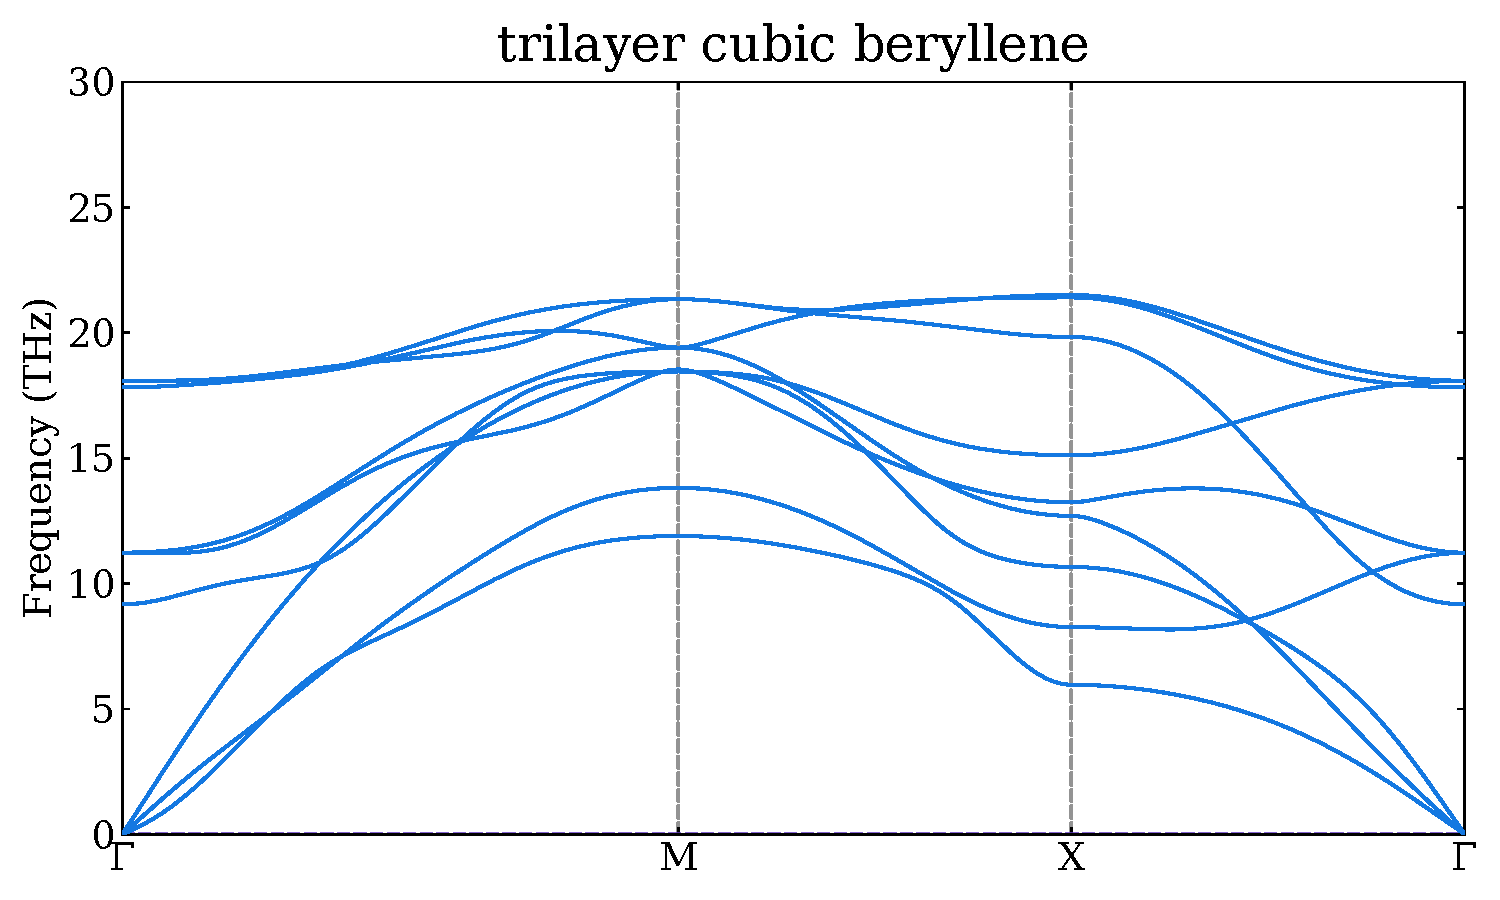
\includegraphics[width=0.40\linewidth]{figures_proj3/phonon_cubic-beryllene-trilayer_thesis.pdf}}%
    &\adjustbox{valign=c}{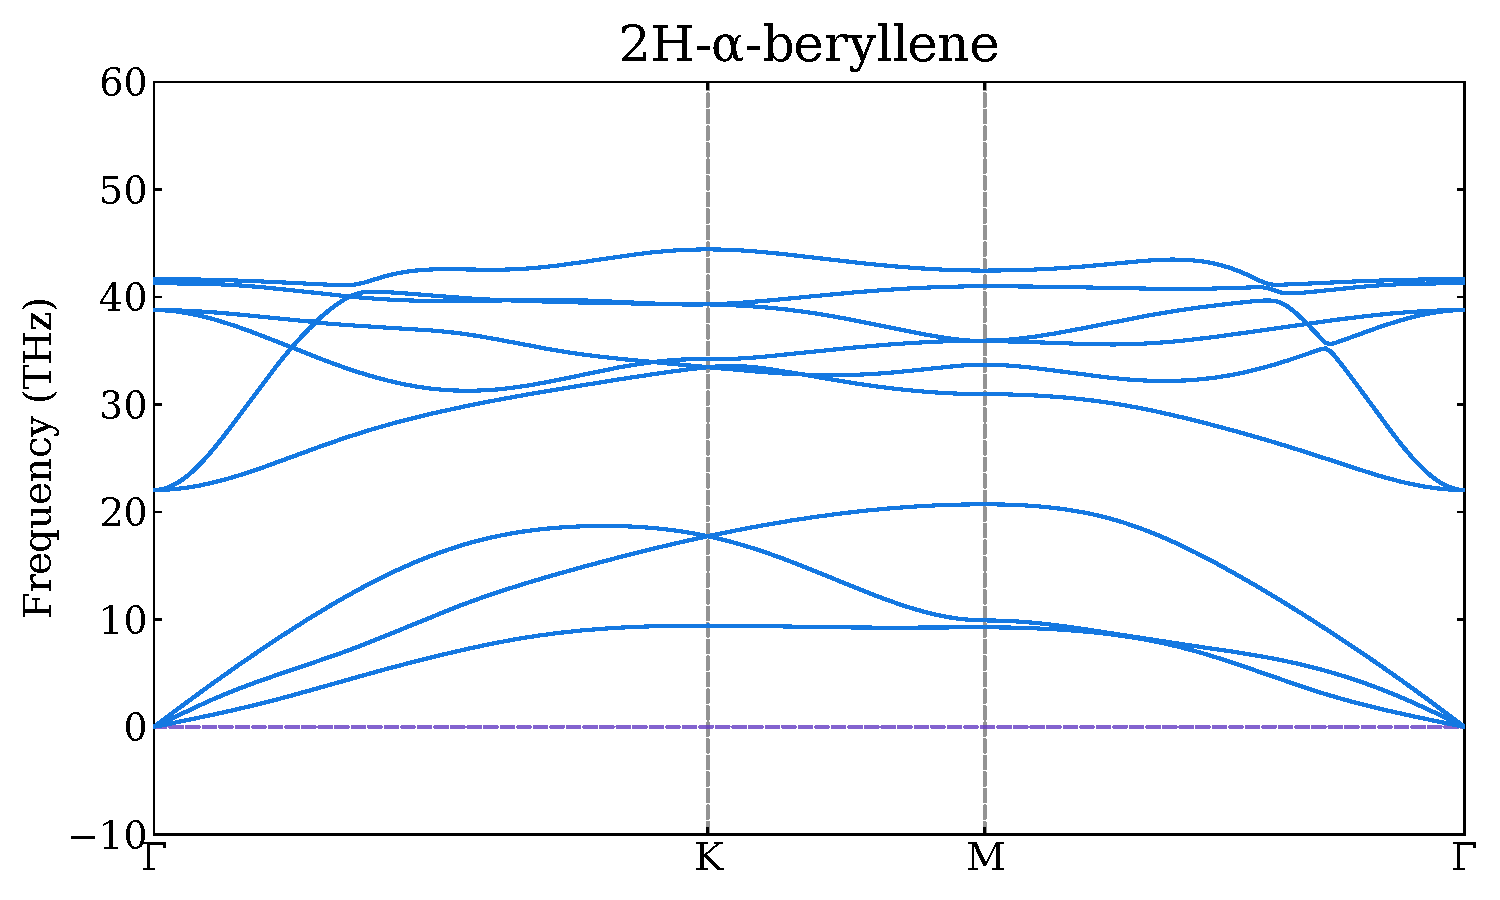
\includegraphics[width=0.40\linewidth]{figures_proj3/phonon_2H-alpha-beryllene_thesis.pdf}}%
    \\\adjustbox{valign=c}{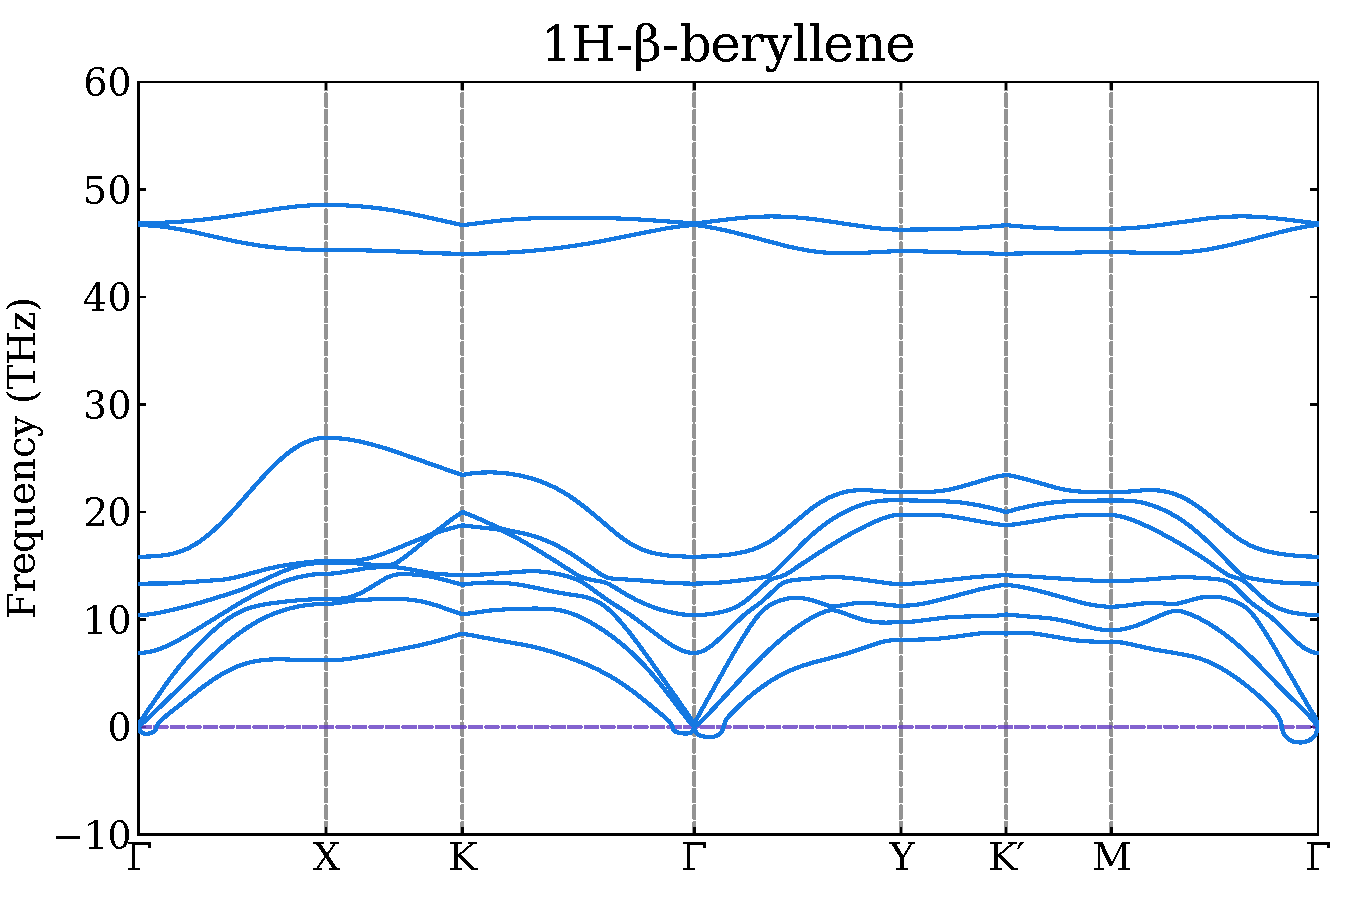
\includegraphics[width=0.40\linewidth]{figures_proj3/phonon_1H-beta-beryllene_thesis.pdf}}%
    &\adjustbox{valign=c}{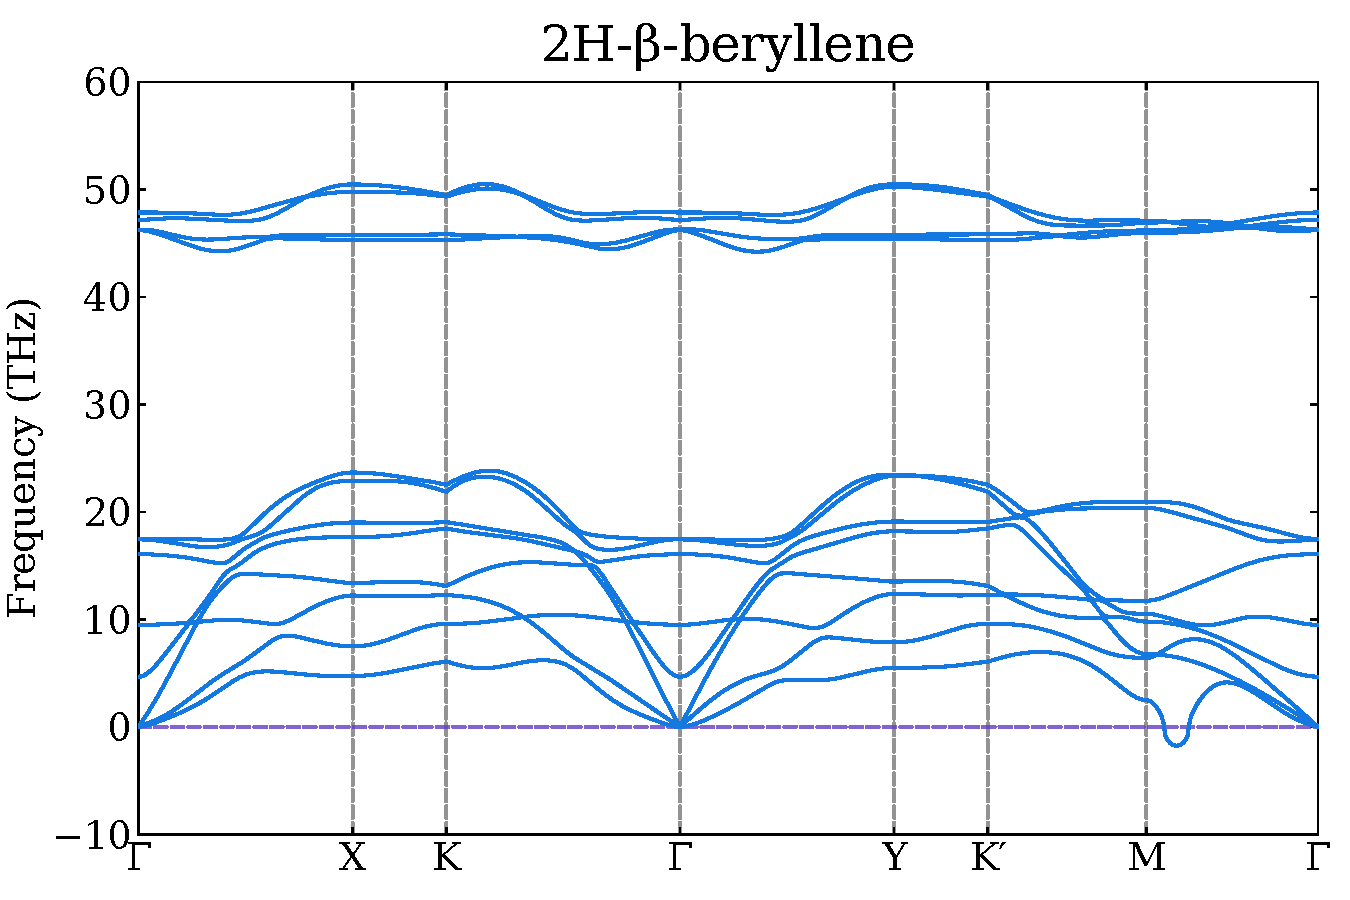
\includegraphics[width=0.40\linewidth]{figures_proj3/phonon_2H-beta-beryllene_thesis.pdf}}%
\end{tabular}
\caption{Phonon-dispersion curves of trilayer cubic beryllene and the hydrogen-functionalized beryllene structures.
Upper left: trilayer cubic beryllene. Upper right: 2H-$\alpha$-beryllene.
Lower left: 1H-$\beta$-beryllene. Lower right: 2H-$\beta$-beryllene.
Imaginary frequencies are shown as negative values.}
\label{fig:proj3_cubic_hydrogenated_phonons}
\end{figure}

Next, we examine the finite-temperature stability of the hydrogen-functionalized structures using \textit{ab initio} molecular dynamics simulations.
The AIMD trajectories and the corresponding atomic structures are shown in figure~\ref{fig:proj3_hydrogenated_aimd}.
For all three hydrogen-functionalized structures,
the total energy fluctuates around a stable average value,
and the temperature fluctuates around the target temperature of \qty{300}{\kelvin}.
The final structures at \qty{5.5}{\pico\second} preserve the beryllene frameworks without structural collapse or hydrogen desorption.
These results support the persistence of the hydrogen-functionalized structures at \qty{300}{\kelvin} over the simulated time interval.

\begin{figure}[!htbp]
\centering
\begin{tabular}{@{}c@{}c@{}}
    \adjustbox{valign=c}{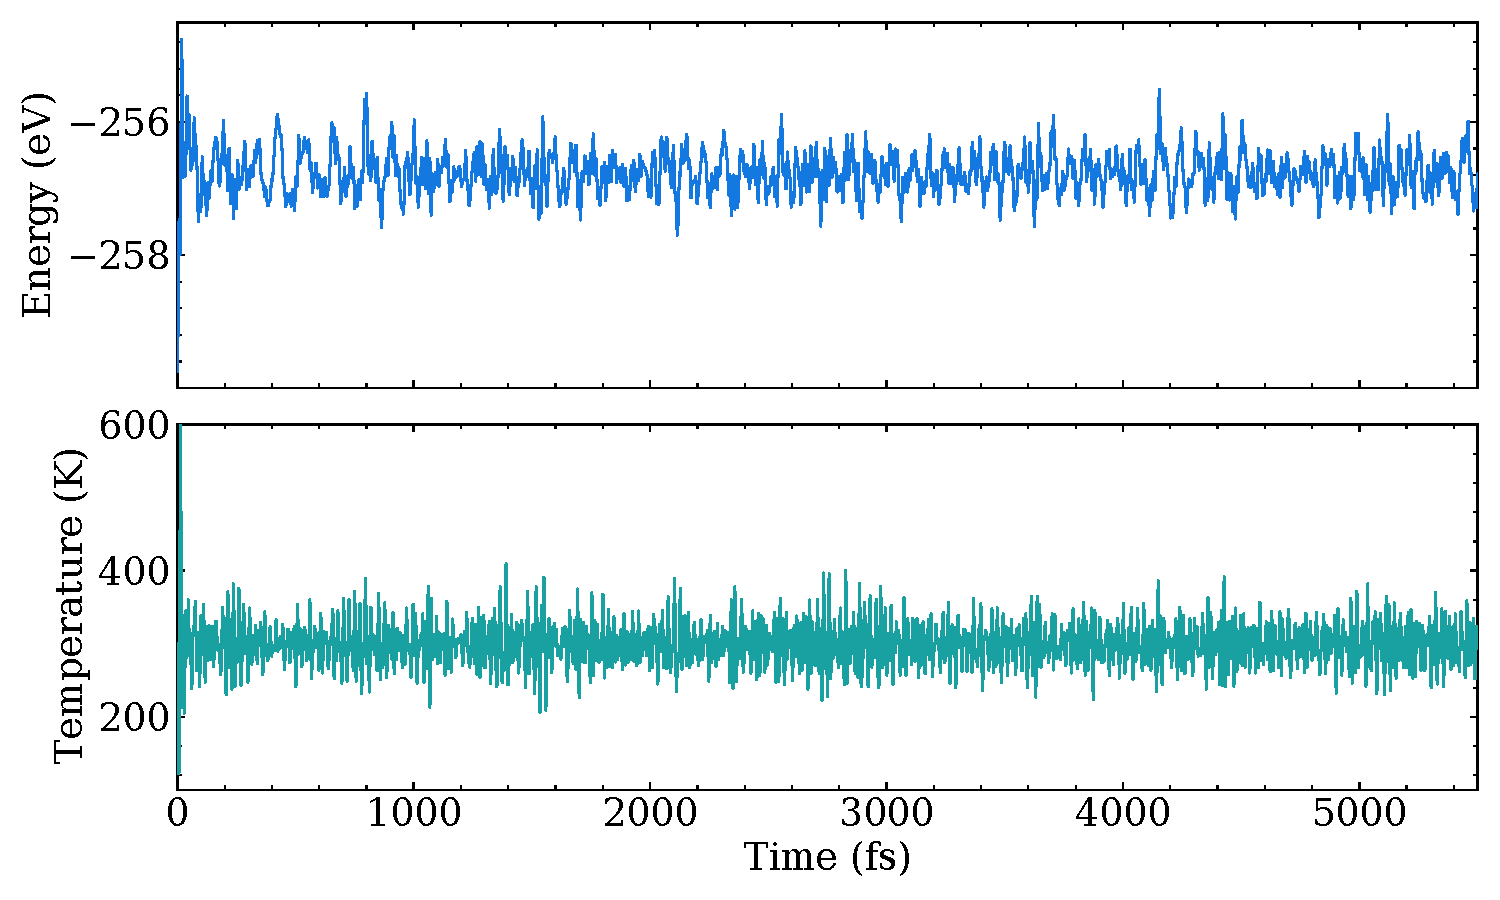
\includegraphics[width=0.50\linewidth]{figures_proj3/aimd_2H-alpha-beryllene_thesis.pdf}}%
    & \adjustbox{valign=c}{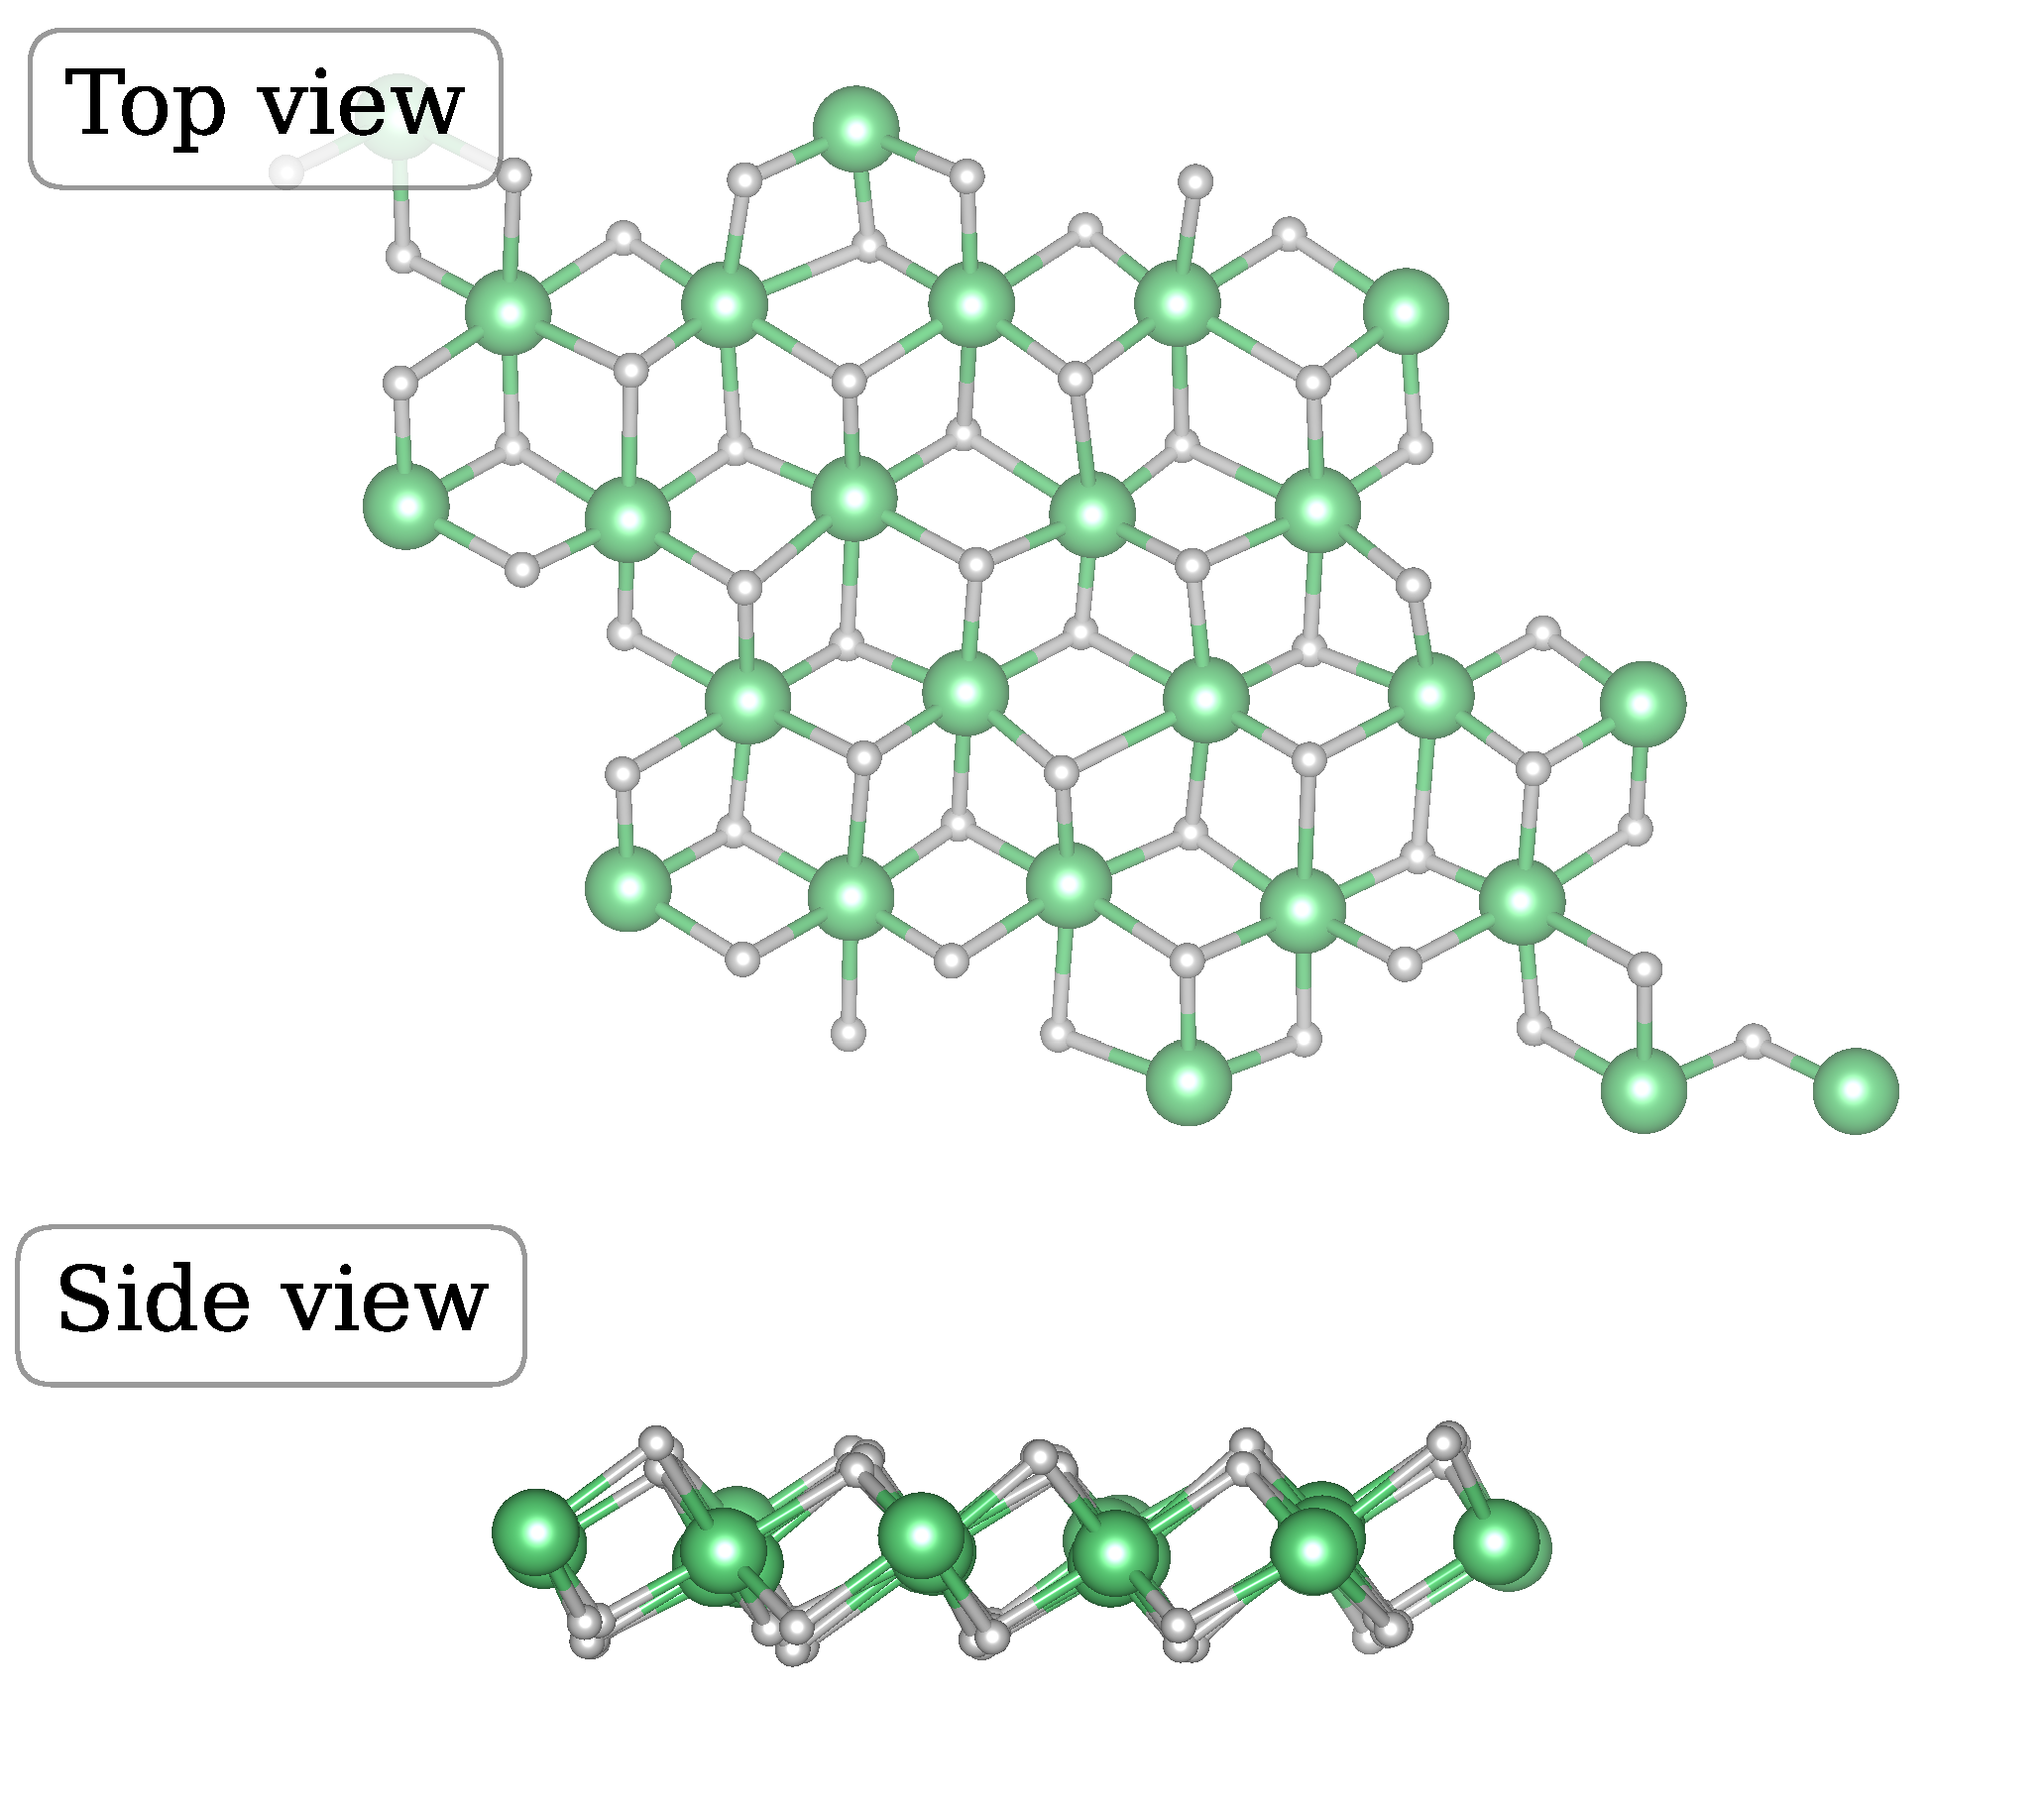
\includegraphics[width=0.30\linewidth]{figures_proj3/structure_2H-alpha-beryllene_thesis.pdf}}\\
    \adjustbox{valign=c}{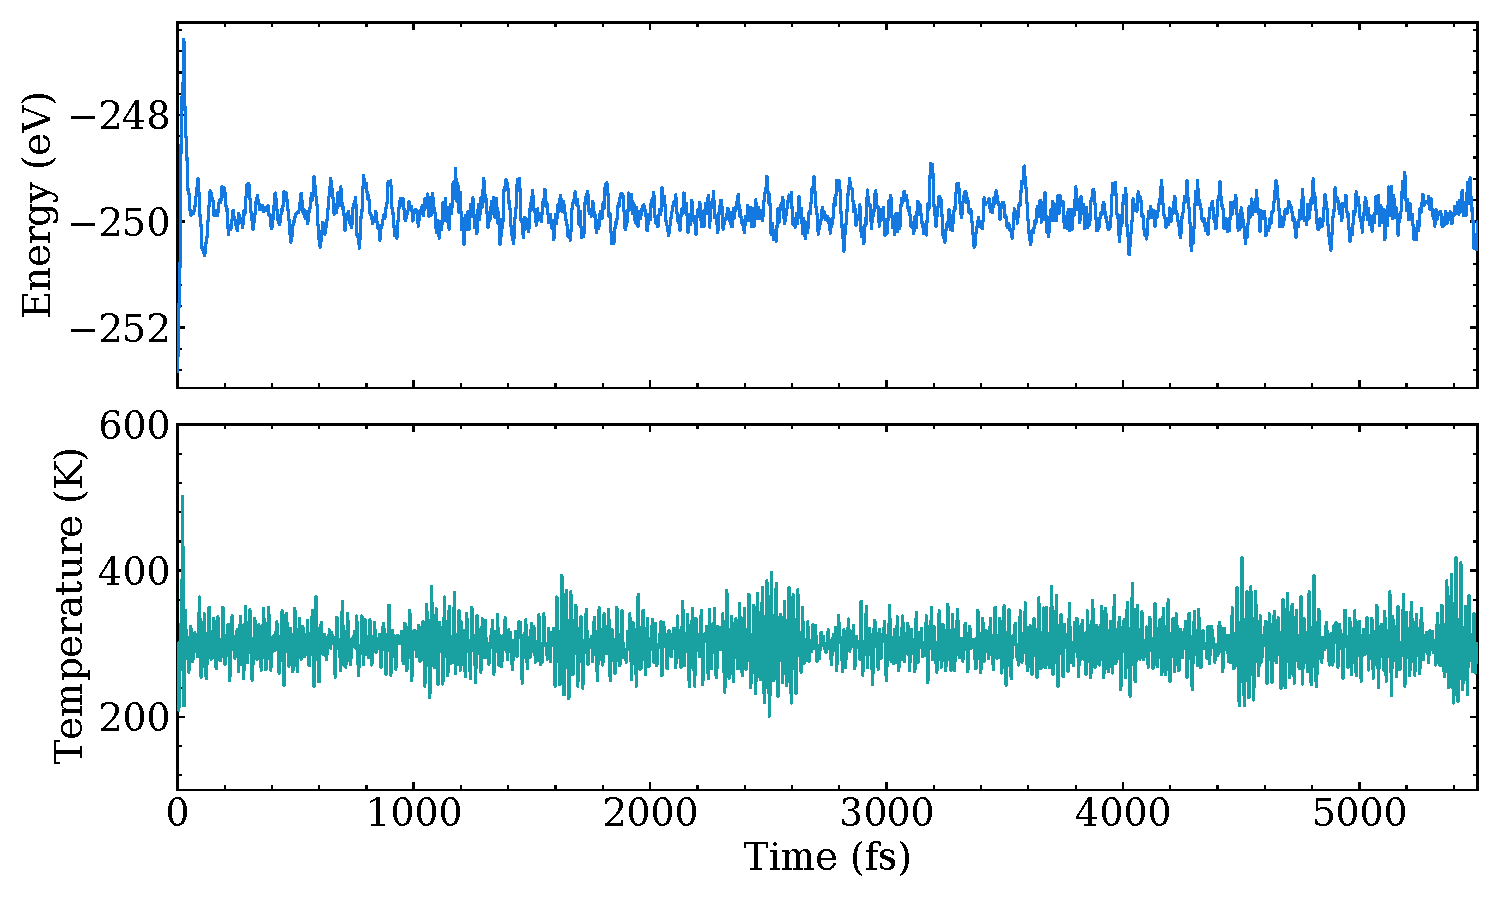
\includegraphics[width=0.50\linewidth]{figures_proj3/aimd_1H-beta-beryllene_thesis.pdf}}%
    & \adjustbox{valign=c}{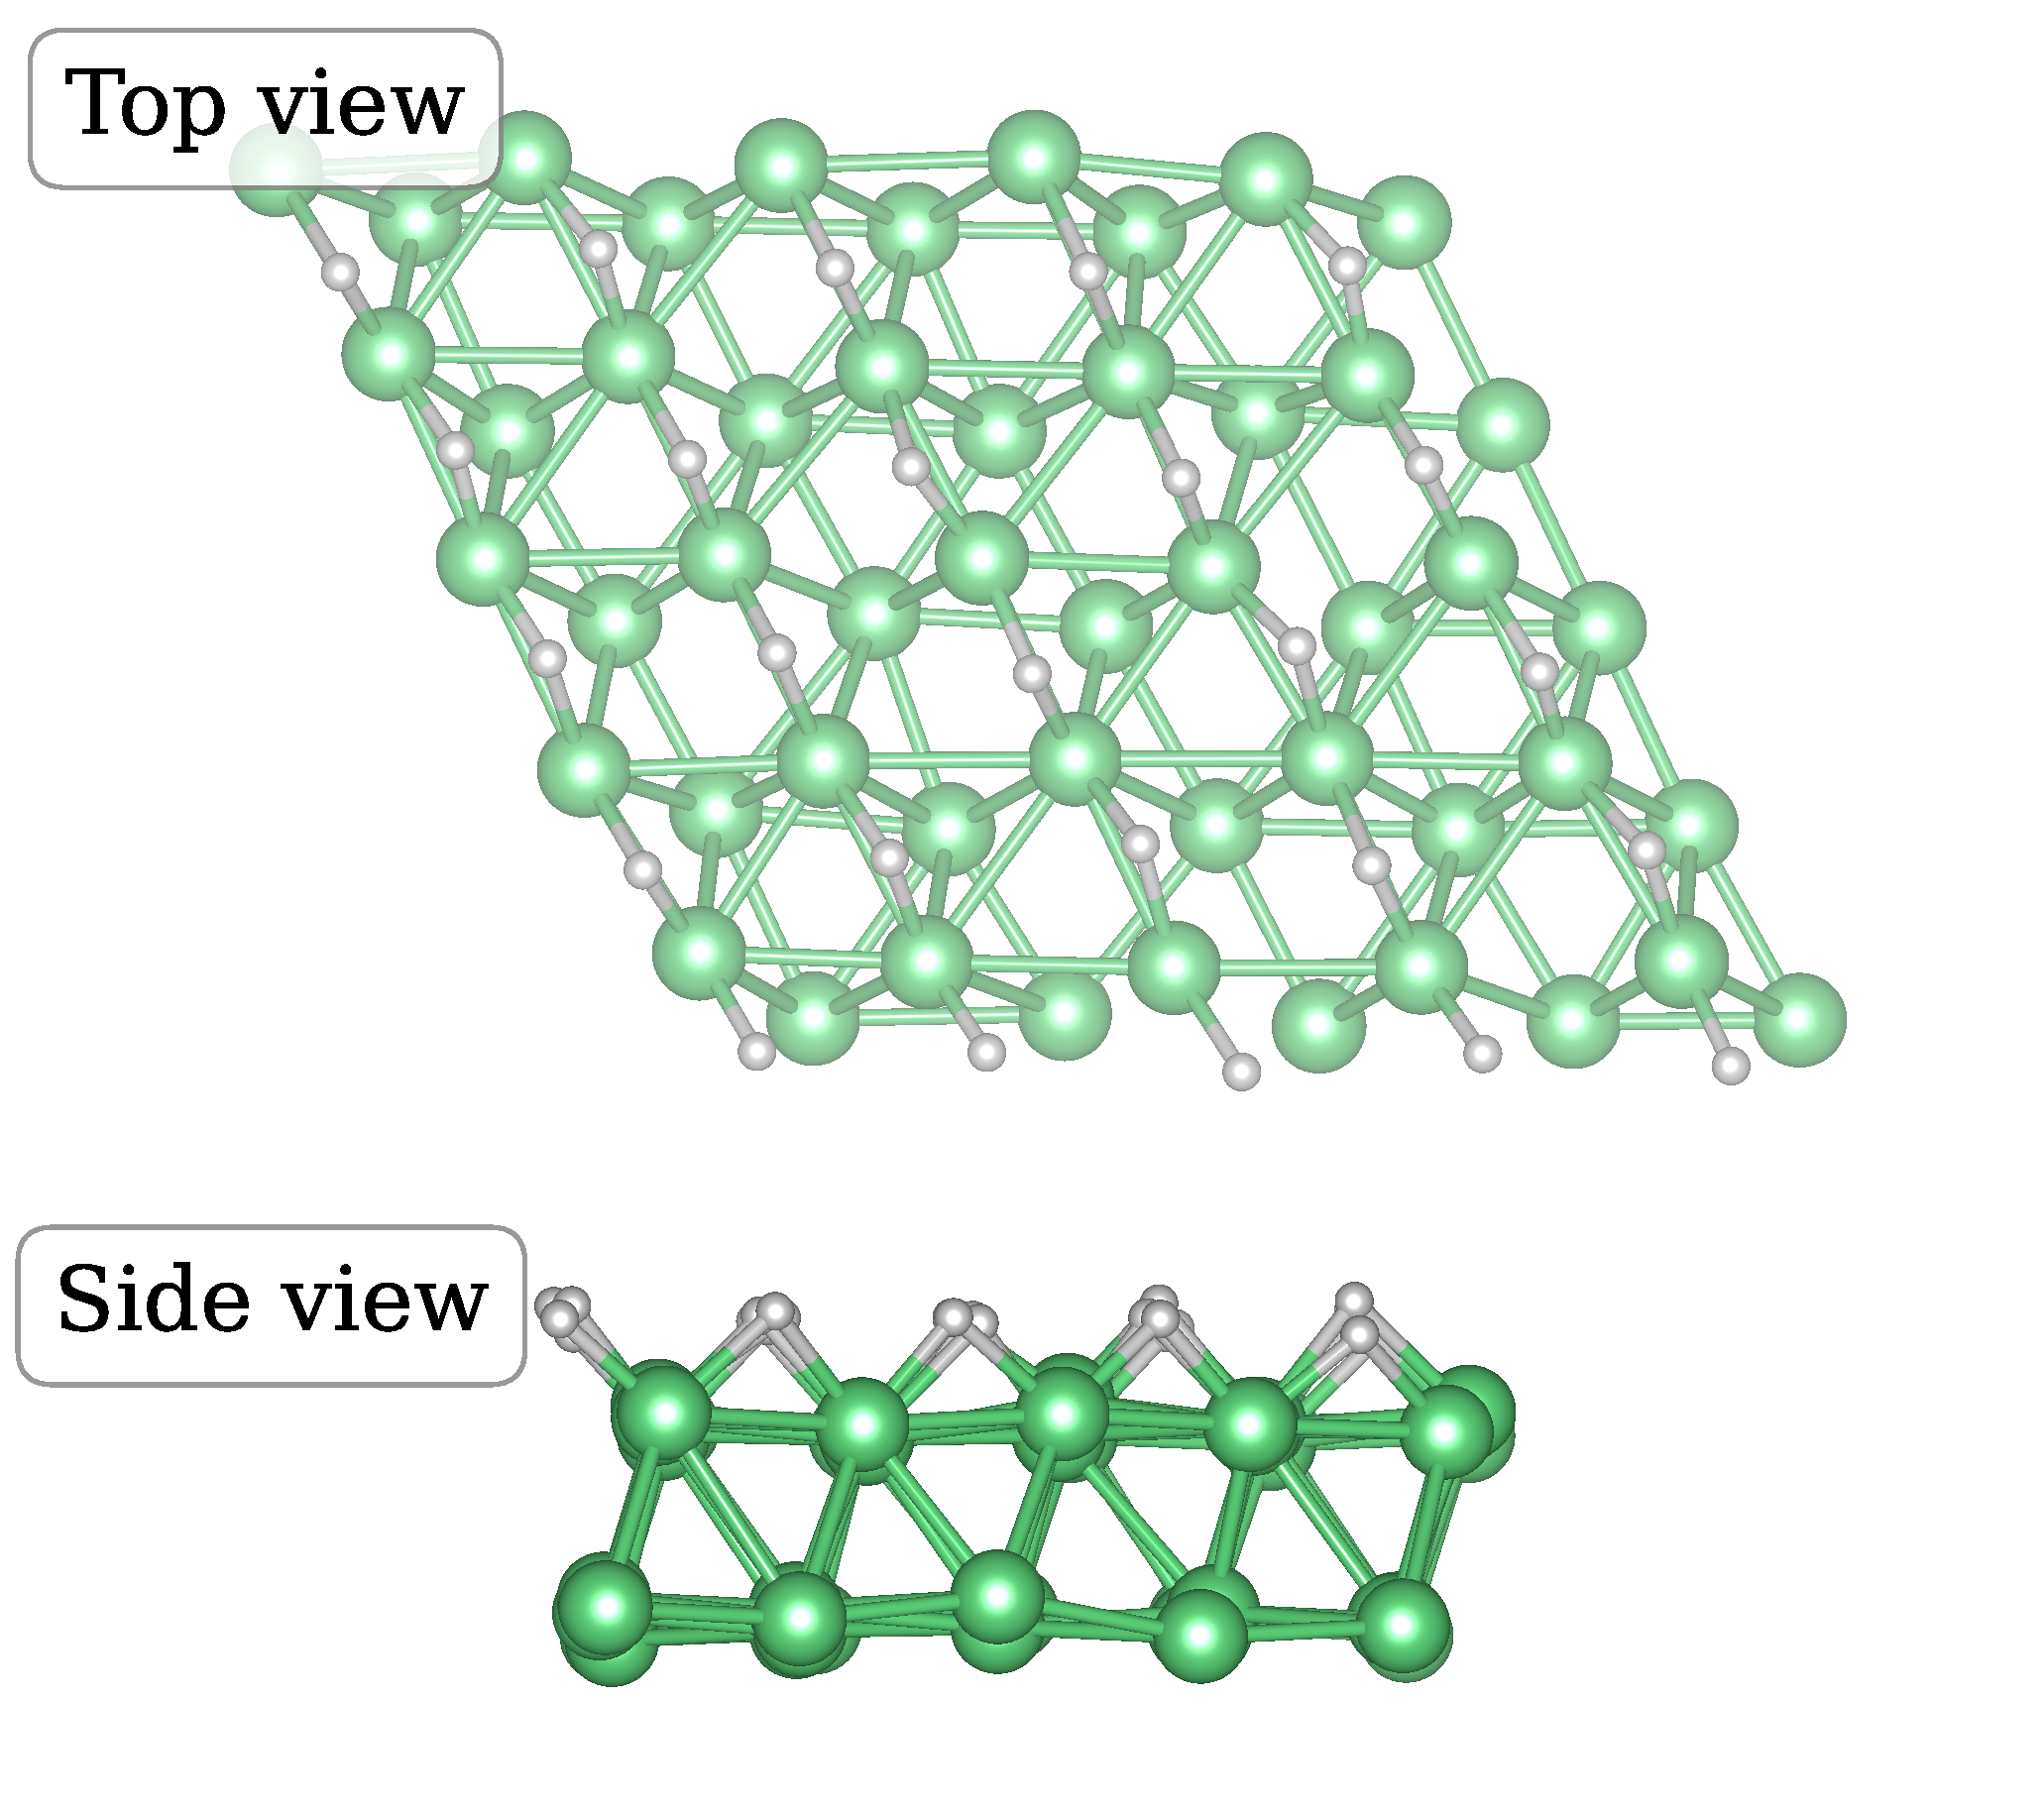
\includegraphics[width=0.30\linewidth]{figures_proj3/structure_1H-beta-beryllene_thesis.pdf}}\\
    \adjustbox{valign=c}{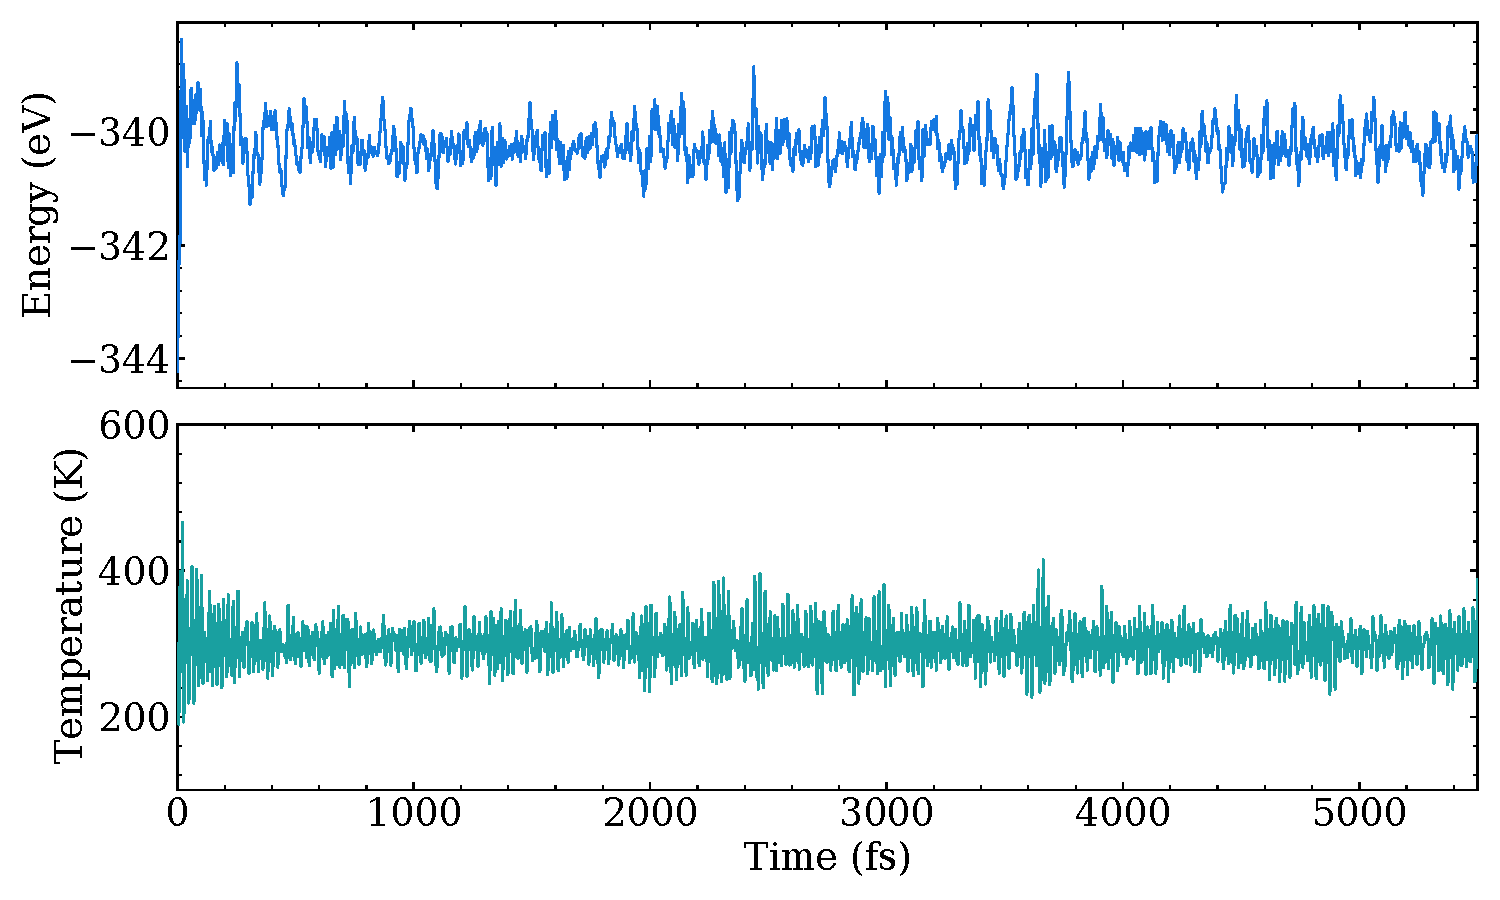
\includegraphics[width=0.50\linewidth]{figures_proj3/aimd_2H-beta-beryllene_thesis.pdf}}%
    & \adjustbox{valign=c}{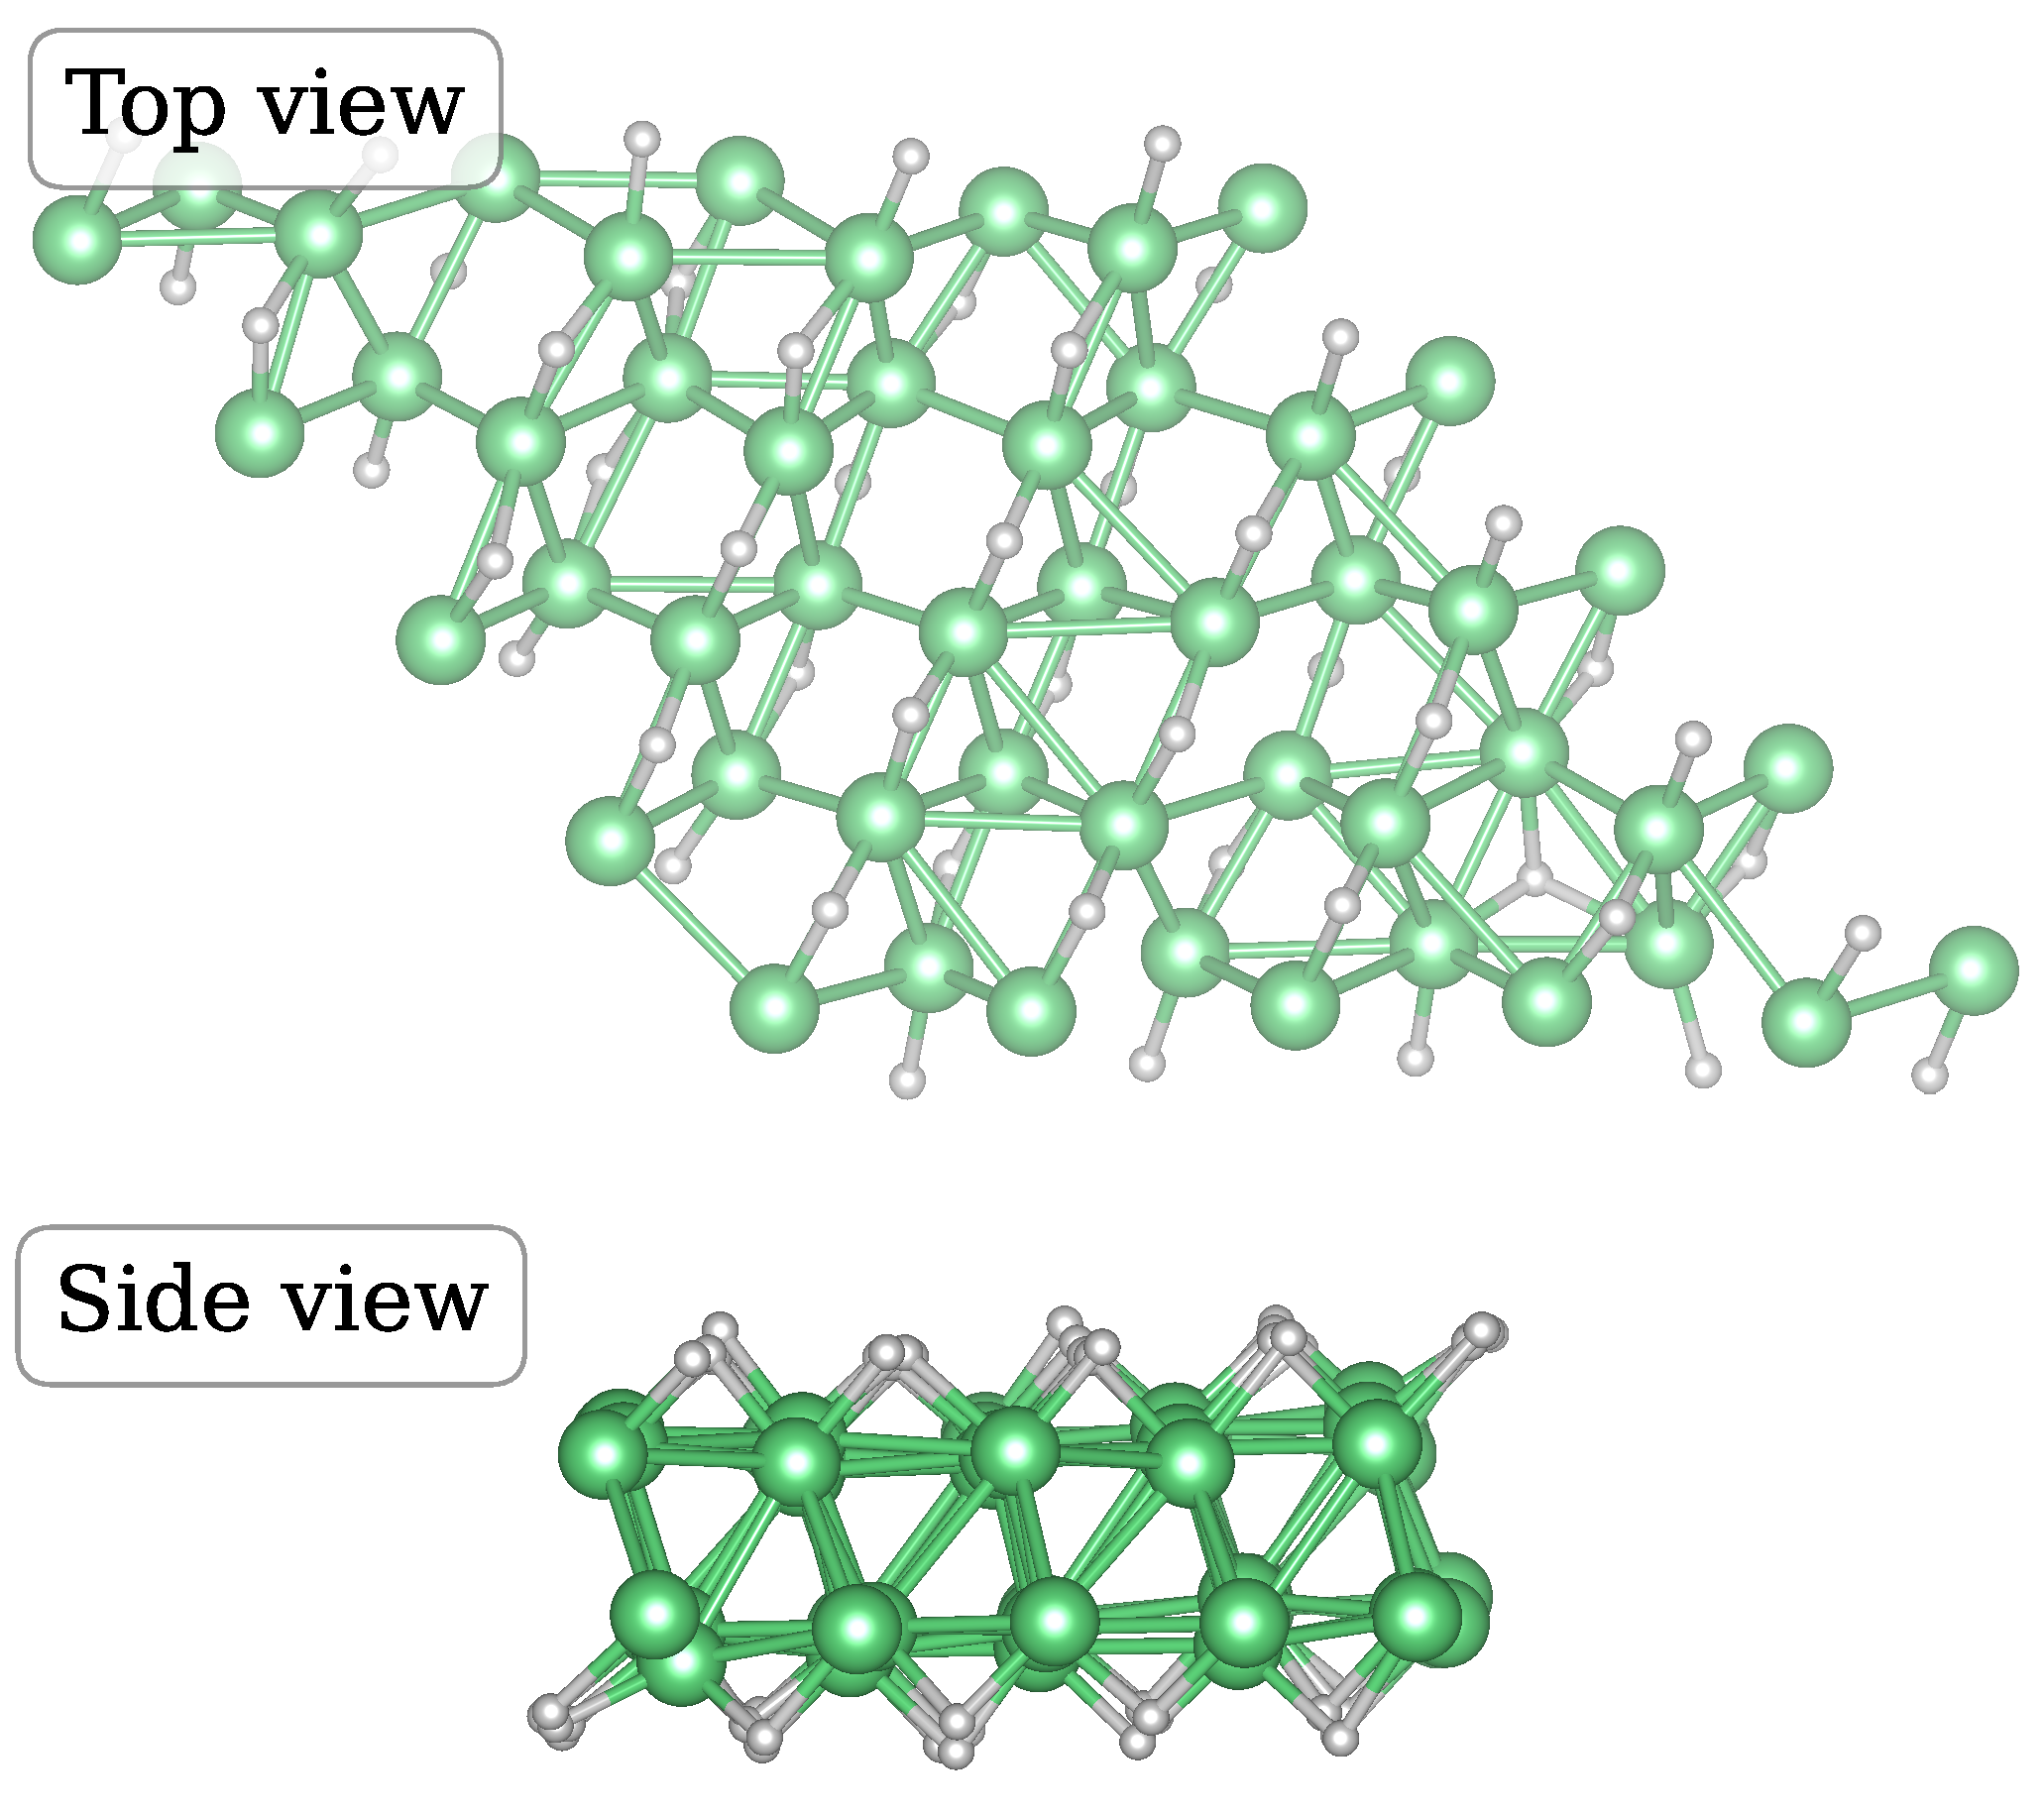
\includegraphics[width=0.30\linewidth]{figures_proj3/structure_2H-beta-beryllene_thesis.pdf}}
\end{tabular}
\caption{\textit{Ab initio} molecular dynamics simulations and corresponding atomic structures of the hydrogen-functionalized beryllene phases.
Upper: 2H-$\alpha$-beryllene.
Middle: 1H-$\beta$-beryllene.
Lower: 2H-$\beta$-beryllene.
For each row,
the left column shows the total energy and temperature as functions of simulation time,
and the right column shows the top and side views of the final structure at \qty{5.5}{\pico\second},
with beryllium in green and hydrogen in grey.}
\label{fig:proj3_hydrogenated_aimd}
\end{figure}

\subsection{Hydrogen adsorption energetics}
\label{3_hydrogen_adsorption_energetics}

The optimized structural parameters of the hydrogen-functionalized structures are listed in table~\ref{tab:proj3_hydrogenated_structural_parameters}.
For 2H-$\alpha$-beryllene,
the in-plane lattice constant increases from \qty{2.129}{\angstrom} in pristine $\alpha$-beryllene to \qty{2.322}{\angstrom} after hydrogen adsorption.
For 1H-$\beta$-beryllene,
hydrogen adsorption breaks the hexagonal symmetry.
The two in-plane lattice constants become \qty{2.322}{\angstrom} and \qty{2.108}{\angstrom},
with an angle of \qty{117}{\degree} between the lattice vectors.
For 2H-$\beta$-beryllene,
the two lattice vectors have the same magnitude of \qty{2.596}{\angstrom},
with an angle of \qty{133}{\degree}.
This geometry forms a rhombic lattice.
The hydrogen adsorption energies relative to \ce{H2} are \qty{-0.33}{\electronvolt},
\qty{-0.07}{\electronvolt},
and \qty{-0.17}{\electronvolt} per hydrogen atom for 2H-$\alpha$-beryllene,
1H-$\beta$-beryllene,
and 2H-$\beta$-beryllene,
respectively.
These negative adsorption energies indicate that hydrogen adsorption is exothermic for all three structures,
although only weakly for 1H-$\beta$-beryllene and 2H-$\beta$-beryllene.

The zero-point energies of the beryllene layers and of the \ce{H2} molecule raise these values to \qty{-0.24}{\electronvolt},
\qty{0.01}{\electronvolt},
and \qty{-0.09}{\electronvolt} per hydrogen atom,
respectively.
At \qty{298.15}{\kelvin} and \qty{1}{\bar} of \ce{H2},
the corresponding adsorption free energies are \qty{-0.08}{\electronvolt},
\qty{0.17}{\electronvolt},
and \qty{0.06}{\electronvolt} per hydrogen atom.
Therefore,
only 2H-$\alpha$-beryllene is thermodynamically stable against \ce{H2} release under ambient conditions.
2H-$\beta$-beryllene requires an equilibrium \ce{H2} pressure of approximately \qty{90}{\bar} at \qty{298.15}{\kelvin},
whereas persistence of 1H-$\beta$-beryllene under ambient conditions would require kinetic trapping.
These energetics are summarized in table~\ref{tab:proj3_hydrogenation_energetics} in section~\ref{3_supplementary}.

2H-$\alpha$-beryllene has the composition of \ce{BeH2}.
We therefore also compare it with two square \ce{BeH2} monolayers relaxed with the same settings.
In a puckered square layer,
each beryllium atom is tetrahedrally coordinated by four bridging hydrogen atoms at \qty{1.468}{\angstrom},
as in bulk \ce{BeH2}.
This puckered layer is \qty{38}{\milli\electronvolt} per formula unit lower in energy than 2H-$\alpha$-beryllene,
whereas a planar square layer is \qty{1.23}{\electronvolt} per formula unit higher.
2H-$\alpha$-beryllene is therefore metastable with respect to the puckered square layer.
The transformation into this layer requires the triangular beryllium lattice to rearrange into a square lattice.
2H-$\alpha$-beryllene may remain kinetically trapped after hydrogenation if the reconstruction barrier is sufficiently high,
but this barrier has not been calculated.
Only these two square configurations are considered,
so this comparison is narrower than a global structure search~\cite{li2018global}.
The polymorph energies are listed in table~\ref{tab:proj3_beh2_polymorphs}.

\begin{table}[!htbp]
\centering
\rowcolors{2}{gray!15}{white}
\begin{adjustbox}{center,max width=1.0\linewidth}
\begin{tabular}{cccccccc}
\hline
\rowcolor{gray!25}
system
& $a$
& $b$
& interlayer Be-Be (\AA)
& H-Be (\AA)
& $E_{\mathrm{ad}}$ (eV)
& angle
& electronic nature \\
\hline
2H-$\alpha$-beryllene
& 2.322 & 2.322 & -- & 1.599 & $-0.33$ & $120^{\circ}$ & semiconductor \\
1H-$\beta$-beryllene
& 2.322 & 2.108 & 1.849 & 1.451 & $-0.07$ & $117^{\circ}$ & metallic \\
2H-$\beta$-beryllene
& 2.596 & 2.596 & 1.786 & 1.446 & $-0.17$ & $133^{\circ}$ & metallic \\
\hline
\end{tabular}
\end{adjustbox}
\caption{Lattice constants $a$ and $b$,
interlayer Be-Be distance, H-Be bond length,
hydrogen adsorption energy $E_{\mathrm{ad}}$ per hydrogen atom relative to \ce{H2},
angle between the two in-plane lattice vectors,
and electronic nature of the hydrogen-functionalized beryllene structures.
The lattice constants, interlayer Be-Be distance,
and H-Be bond length are given in \si{\angstrom},
while the adsorption energy is given in \si{\electronvolt}.}
\label{tab:proj3_hydrogenated_structural_parameters}
\end{table}

\subsection{Electronic properties}
\label{3_electronic_properties}

We now examine the electronic properties of pristine and hydrogen-functionalized beryllene structures.
The band structures of pristine $\alpha$-beryllene and $\beta$-beryllene are shown in figure~\ref{fig:proj3_band_structures} in section~\ref{3_supplementary},
and agree well with previous calculations~\cite{li2023coexistence}.
The band structures of trilayer cubic beryllene and the hydrogen-functionalized structures are shown in figure~\ref{fig:proj3_band_structures_cubic_hydrogenated}.

Trilayer cubic beryllene shows metallic behaviour,
with multiple bands crossing the Fermi level.
The bands near the Fermi level show moderate dispersion,
which suggests delocalized electronic states and good in-plane conductivity.
Around the $\Gamma$,
$\mathrm{M}$,
and $\mathrm{X}$ points,
noticeable band splitting appears,
consistent with interlayer coupling in the trilayer structure.
The coexistence of relatively flat bands and dispersive unoccupied bands at higher energies further indicates a mixture of localized and itinerant electronic states.

Hydrogen functionalization changes the electronic structure differently for the $\alpha$ and $\beta$ phases.
For 2H-$\alpha$-beryllene,
the band structure shows a wide indirect band gap of \qty{4.84}{\electronvolt} at the PBE level.
As PBE generally underestimates band gaps,
we also calculate its band structure with the HSE06 hybrid functional.
HSE06 increases the indirect band gap to \qty{6.00}{\electronvolt},
while the valence-band maximum and the conduction-band minimum remain at the same wave vectors.
In contrast,
both 1H-$\beta$-beryllene and 2H-$\beta$-beryllene remain metallic,
with bands crossing the Fermi level.
These results show that hydrogen functionalization opens a large gap in $\alpha$-beryllene,
whereas the hydrogen-functionalized $\beta$-beryllene structures preserve their metallic character.

\begin{figure}[!htbp]
\centering
\begin{tabular}{@{}cc@{}}
    \adjustbox{valign=c}{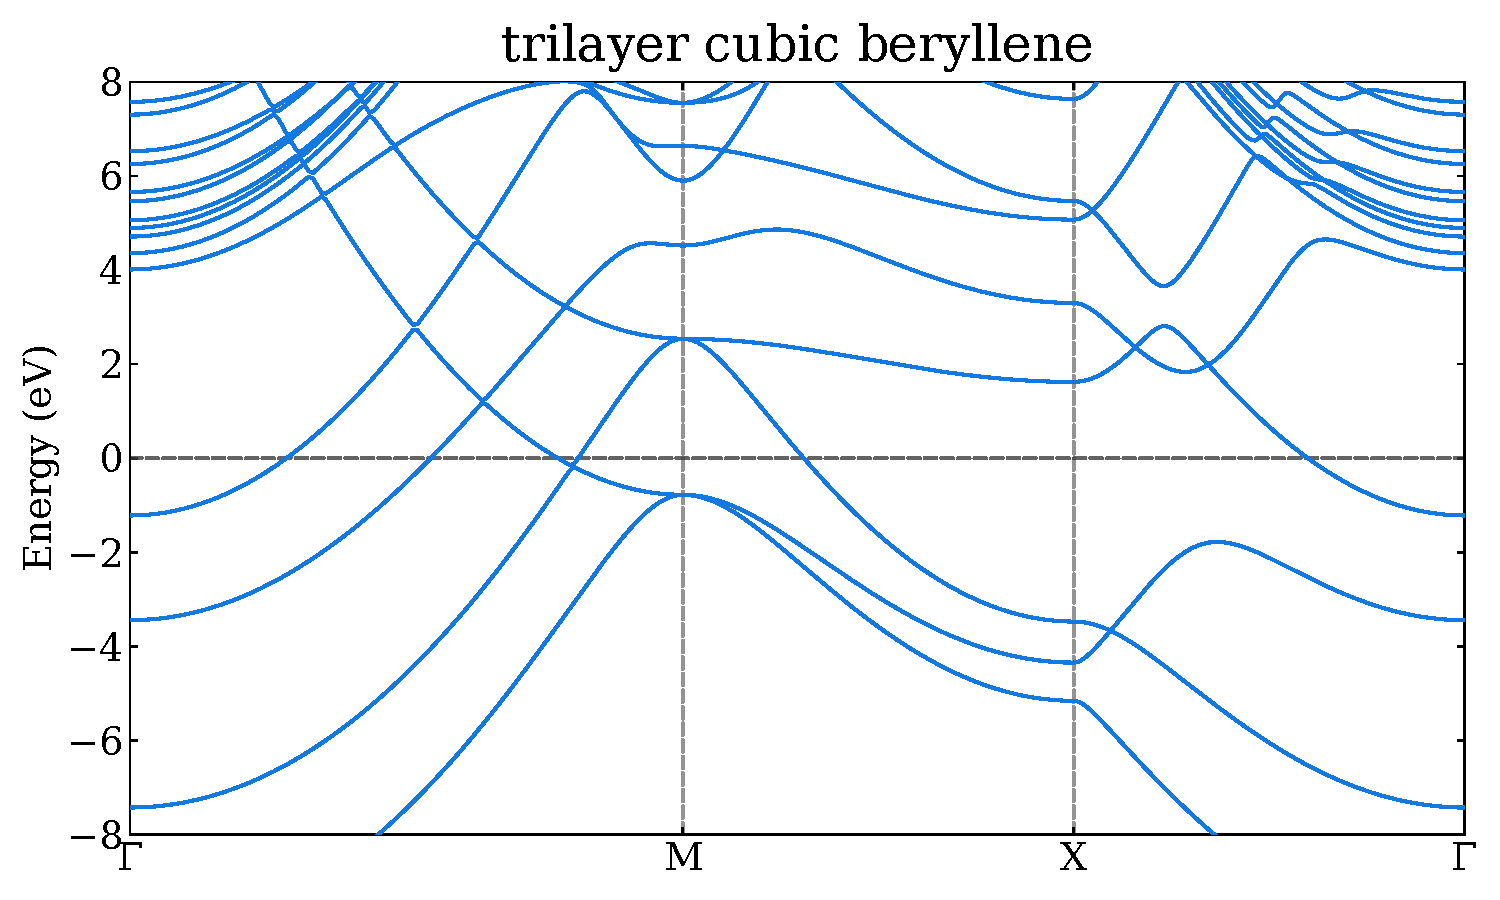
\includegraphics[width=0.40\linewidth]{figures_proj3/bands_cubic-beryllene-trilayer_thesis.pdf}}&
    \adjustbox{valign=c}{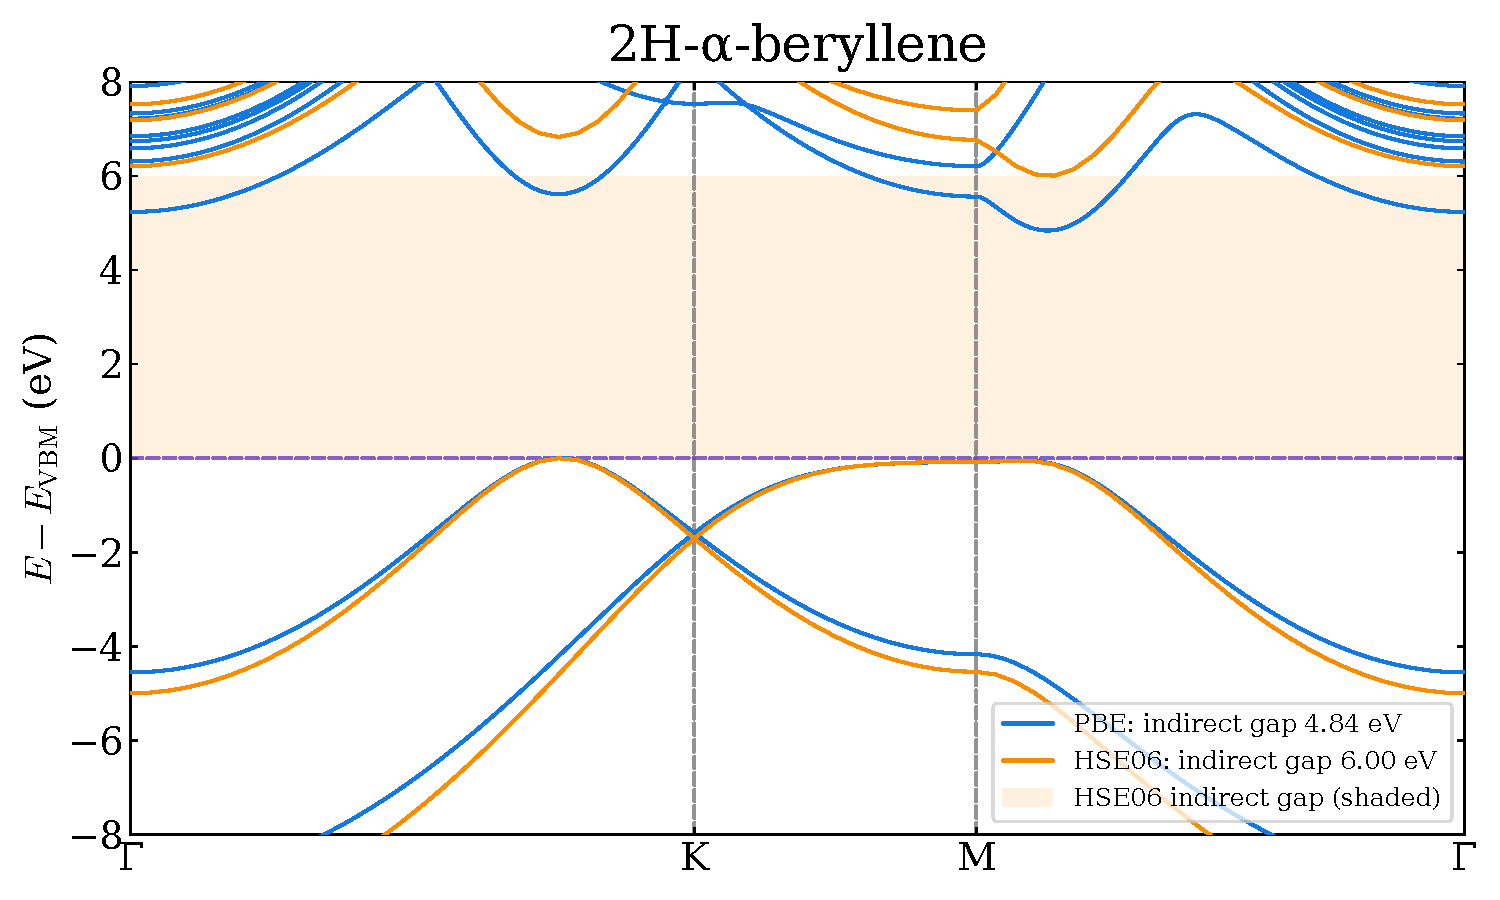
\includegraphics[width=0.40\linewidth]{figures_proj3/bands_2H-alpha-beryllene_thesis.pdf}}\\
    \adjustbox{valign=c}{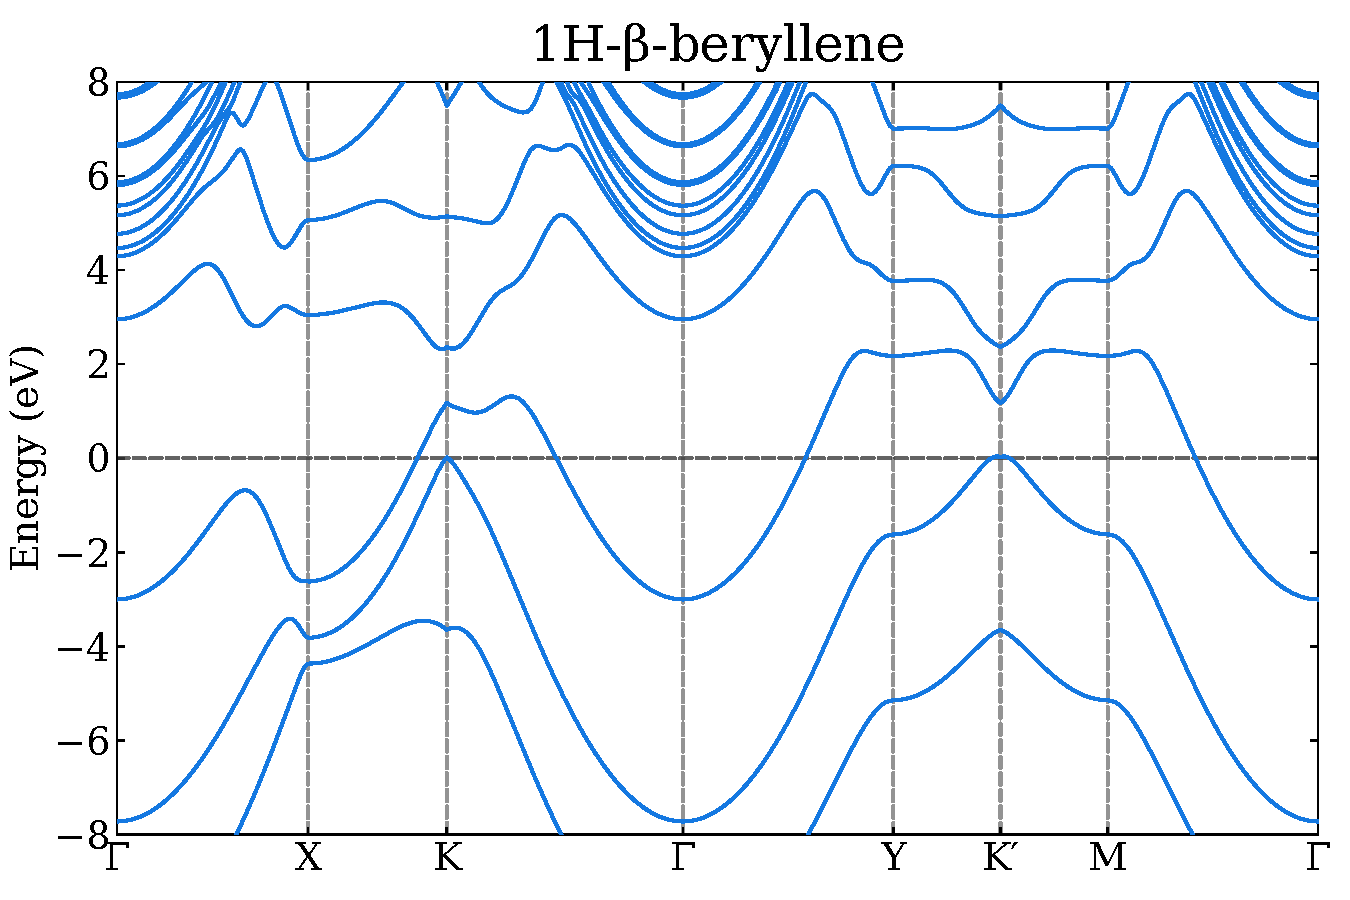
\includegraphics[width=0.40\linewidth]{figures_proj3/bands_1H-beta-beryllene_thesis.pdf}}&
    \adjustbox{valign=c}{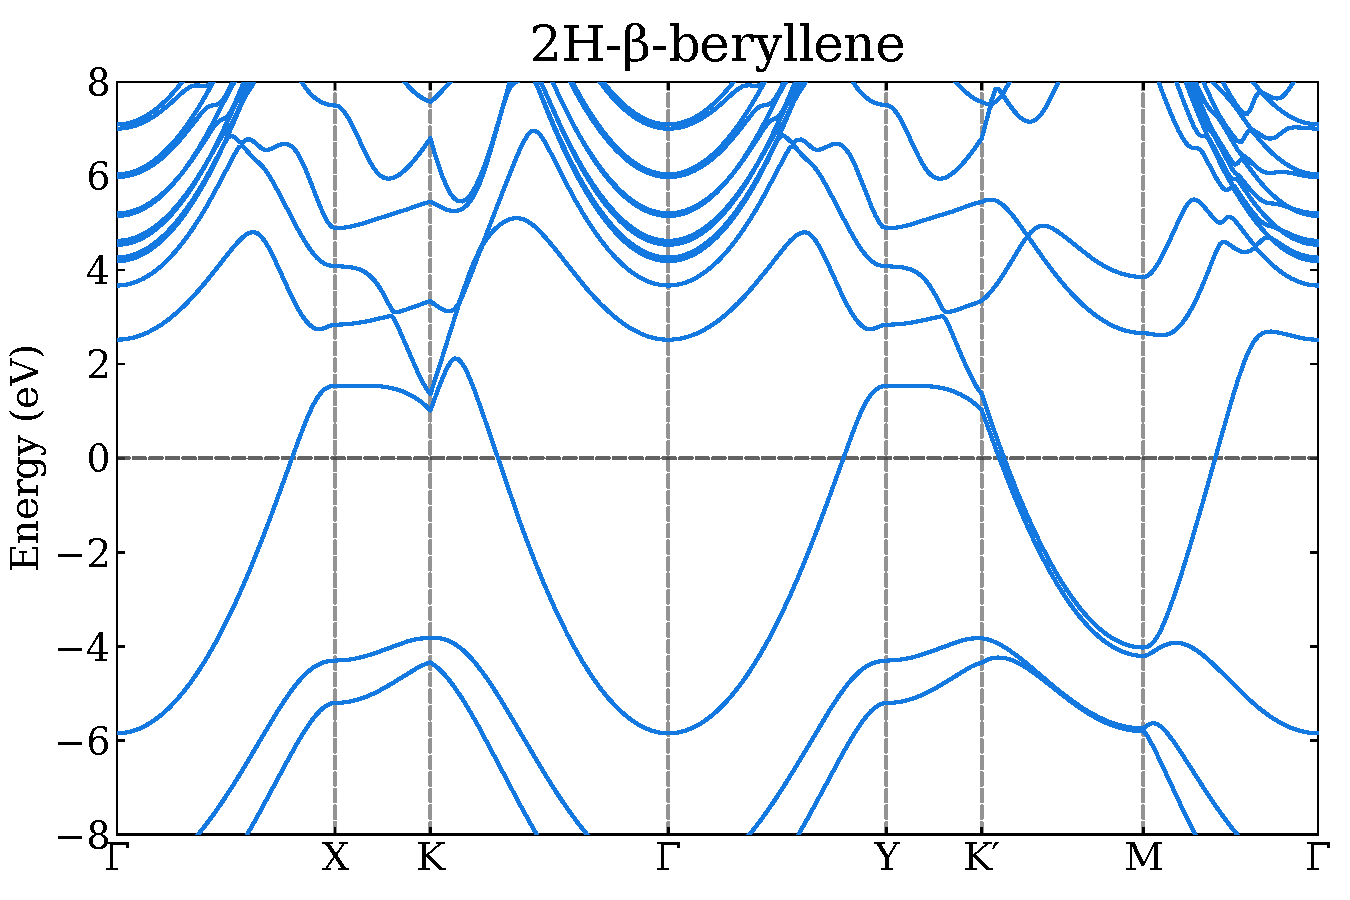
\includegraphics[width=0.40\linewidth]{figures_proj3/bands_2H-beta-beryllene_thesis.pdf}}
\end{tabular}
\caption{Band structures of trilayer cubic beryllene and the hydrogen-functionalized beryllene structures.
Upper left: trilayer cubic beryllene. Upper right: 2H-$\alpha$-beryllene.
Lower left: 1H-$\beta$-beryllene. Lower right: 2H-$\beta$-beryllene.
For 1H-$\beta$-beryllene and 2H-$\beta$-beryllene,
the path $\Gamma$--$\mathrm{X}$--$\mathrm{K}$--$\Gamma$--$\mathrm{Y}$--$\mathrm{K}'$--$\mathrm{M}$--$\Gamma$ passes through all four time-reversal invariant momenta and the zone corners $\mathrm{K}$ and $\mathrm{K}'$,
as for the phonon dispersions in figure~\ref{fig:proj3_cubic_hydrogenated_phonons}.
For 2H-$\alpha$-beryllene,
the PBE (blue) and HSE06 (orange) bands are each aligned at their valence-band maximum.}
\label{fig:proj3_band_structures_cubic_hydrogenated}
\end{figure}

The density of states further supports the band-structure interpretation.
Figure~\ref{fig:proj3_dos_cubic_trilayer} compares the total density of states of bulk bcc beryllium and trilayer cubic beryllene.
Trilayer cubic beryllene has a finite density of states at the Fermi level,
consistent with its metallic band structure.

\begin{figure}[!htbp]
\centering
    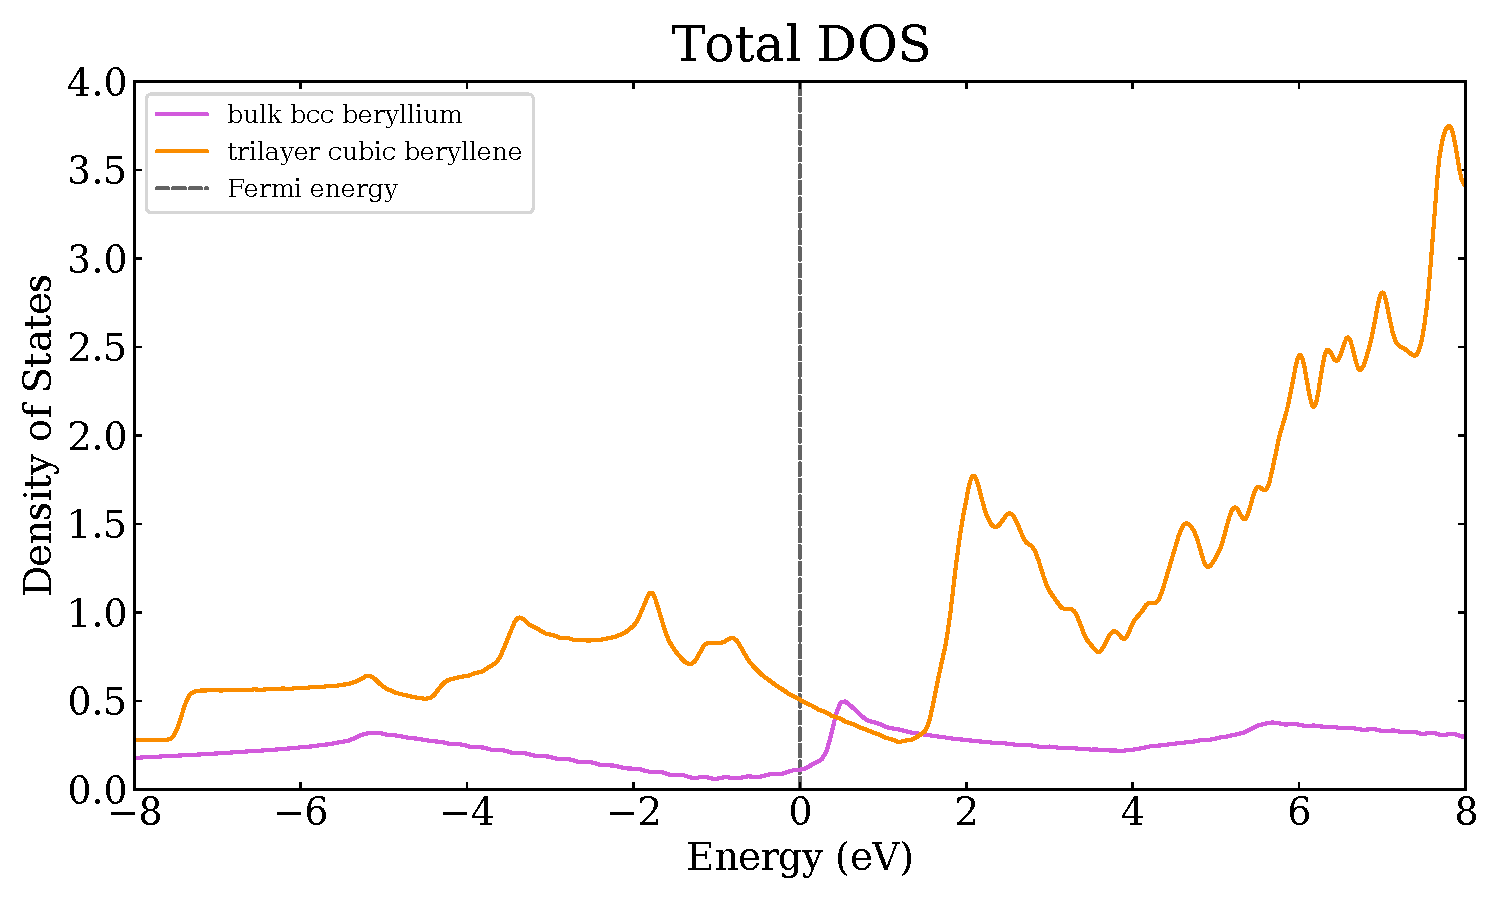
\includegraphics[width=0.6\linewidth]{figures_proj3/dos_cubic-family_thesis.pdf}
\caption{Total density of states of bulk bcc beryllium and trilayer cubic beryllene.}
\label{fig:proj3_dos_cubic_trilayer}
\end{figure}

The total and projected densities of states of pristine and hydrogen-functionalized beryllene structures are shown in figure~\ref{fig:proj3_dos_hydrogenated}.
For 2H-$\alpha$-beryllene,
the density of states vanishes around the Fermi level,
consistent with the wide-gap semiconducting band structure.
For 1H-$\beta$-beryllene and 2H-$\beta$-beryllene,
the finite density of states at the Fermi level confirms their metallic behaviour.
The projected densities of states show strong hybridization among beryllium $s$ and $p$ states,
together with the hydrogen $1s$ state in the hydrogen-functionalized structures.
This hybridization reflects the modification of the local bonding environment after hydrogen functionalization.

\begin{figure}[!htbp]
\centering
\begin{tabular}{@{}cc@{}}
    \adjustbox{valign=c}{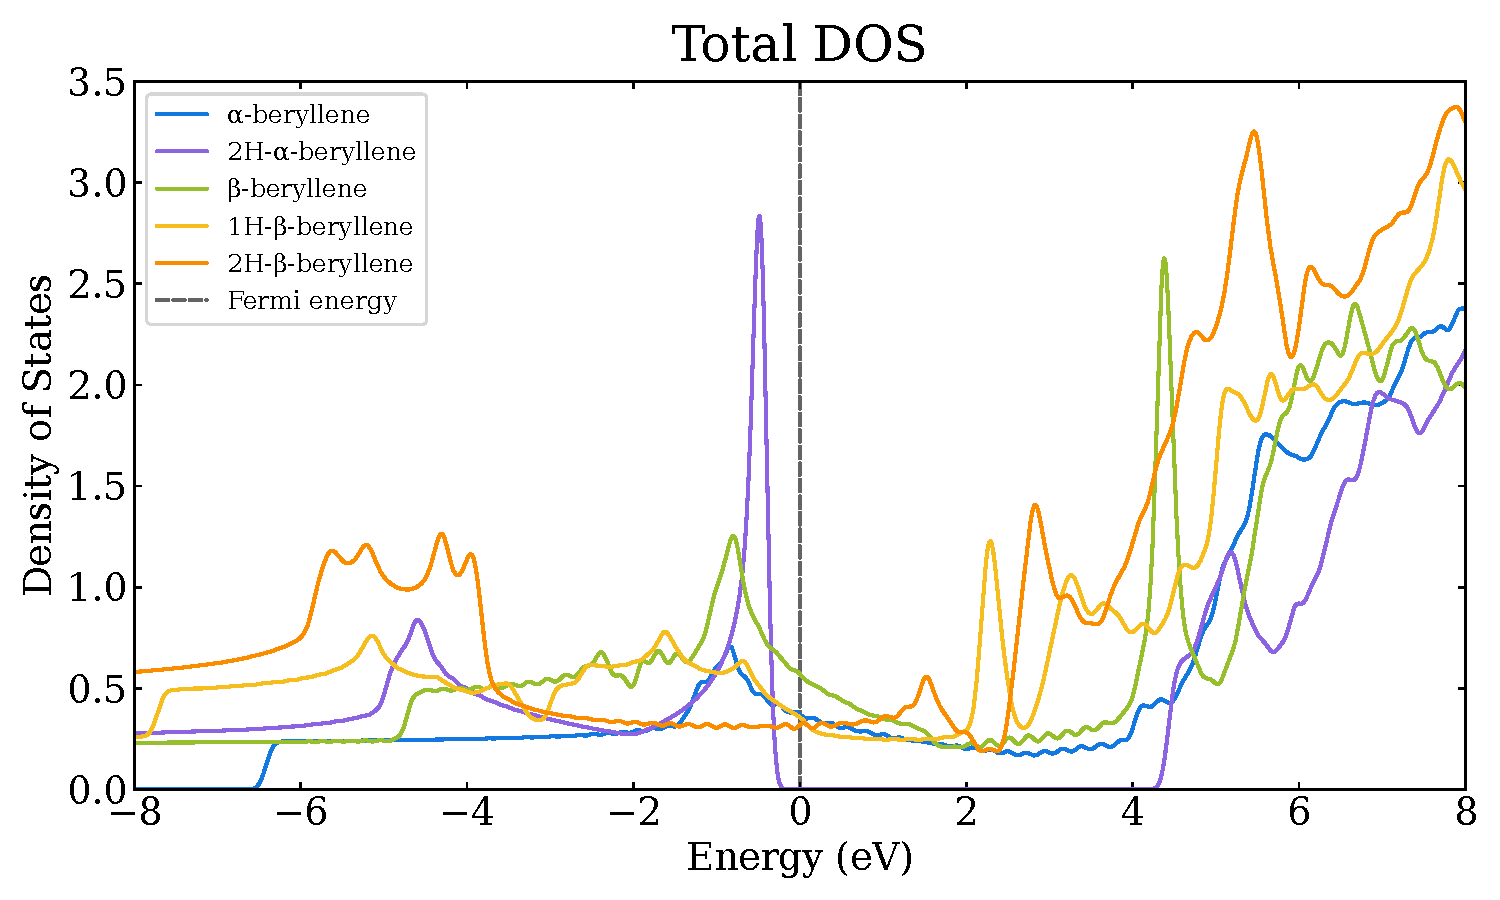
\includegraphics[width=0.40\linewidth]{figures_proj3/dos_hydrogenated_thesis.pdf}}&
    \adjustbox{valign=c}{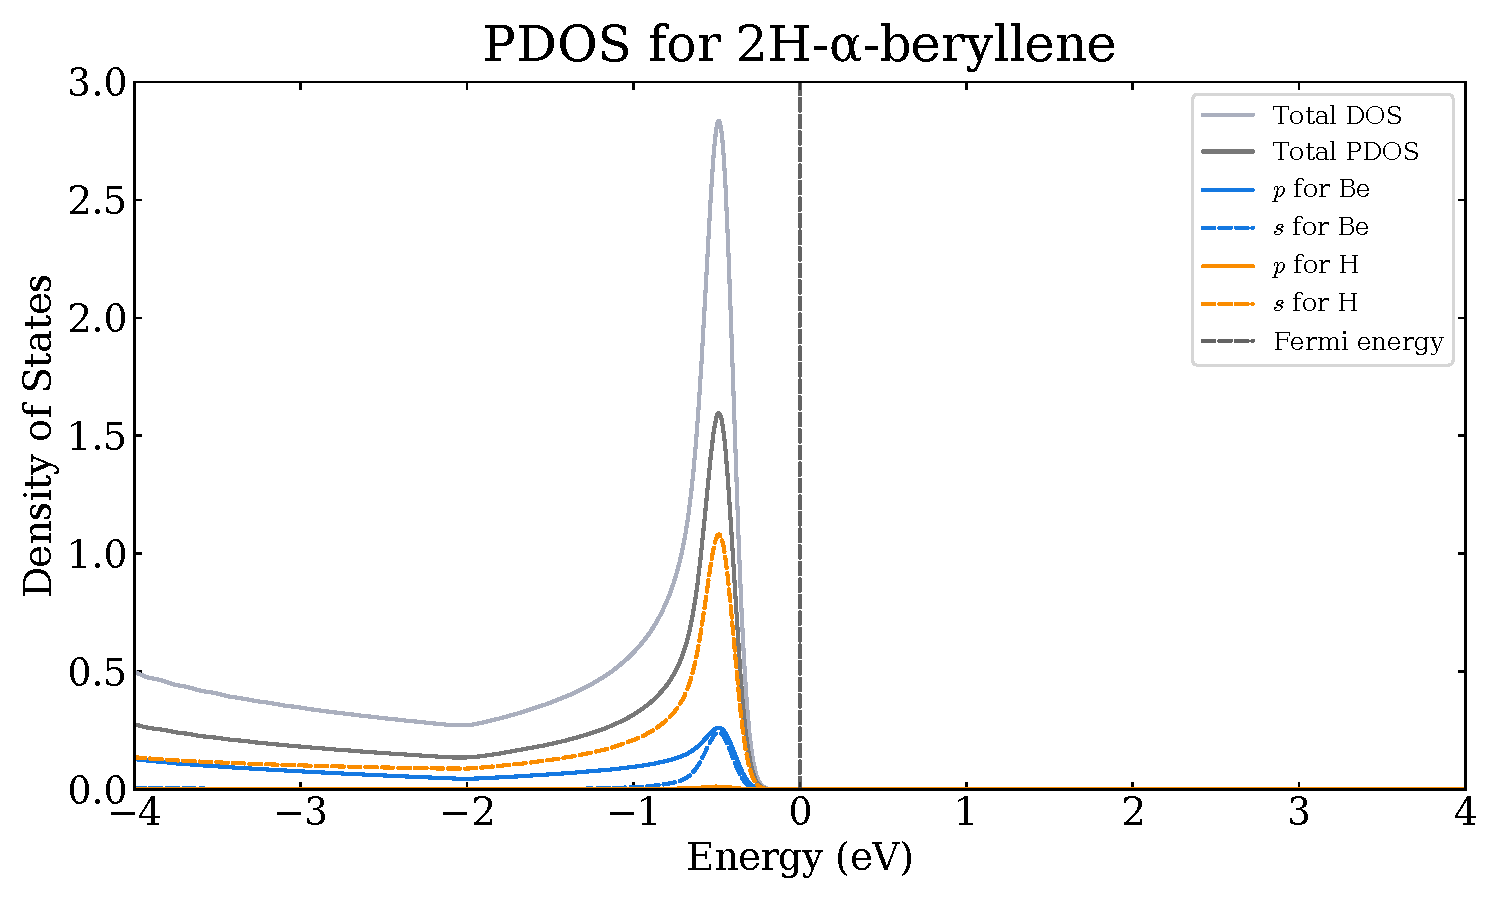
\includegraphics[width=0.40\linewidth]{figures_proj3/pdos_2H-alpha-beryllene_thesis.pdf}}\\
    \adjustbox{valign=c}{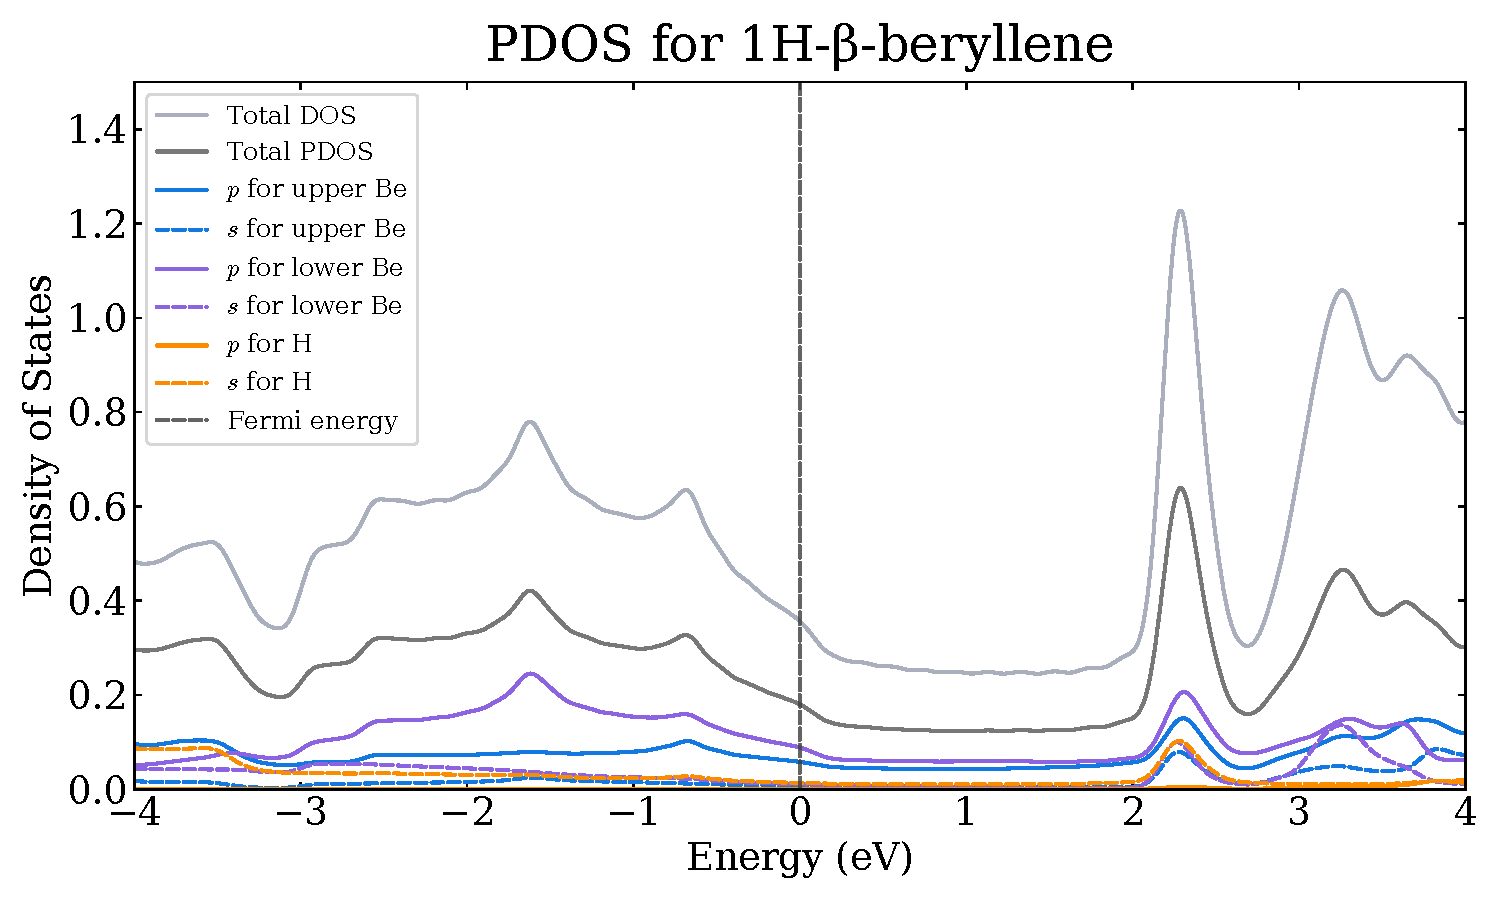
\includegraphics[width=0.40\linewidth]{figures_proj3/pdos_1H-beta-beryllene_thesis.pdf}}&
    \adjustbox{valign=c}{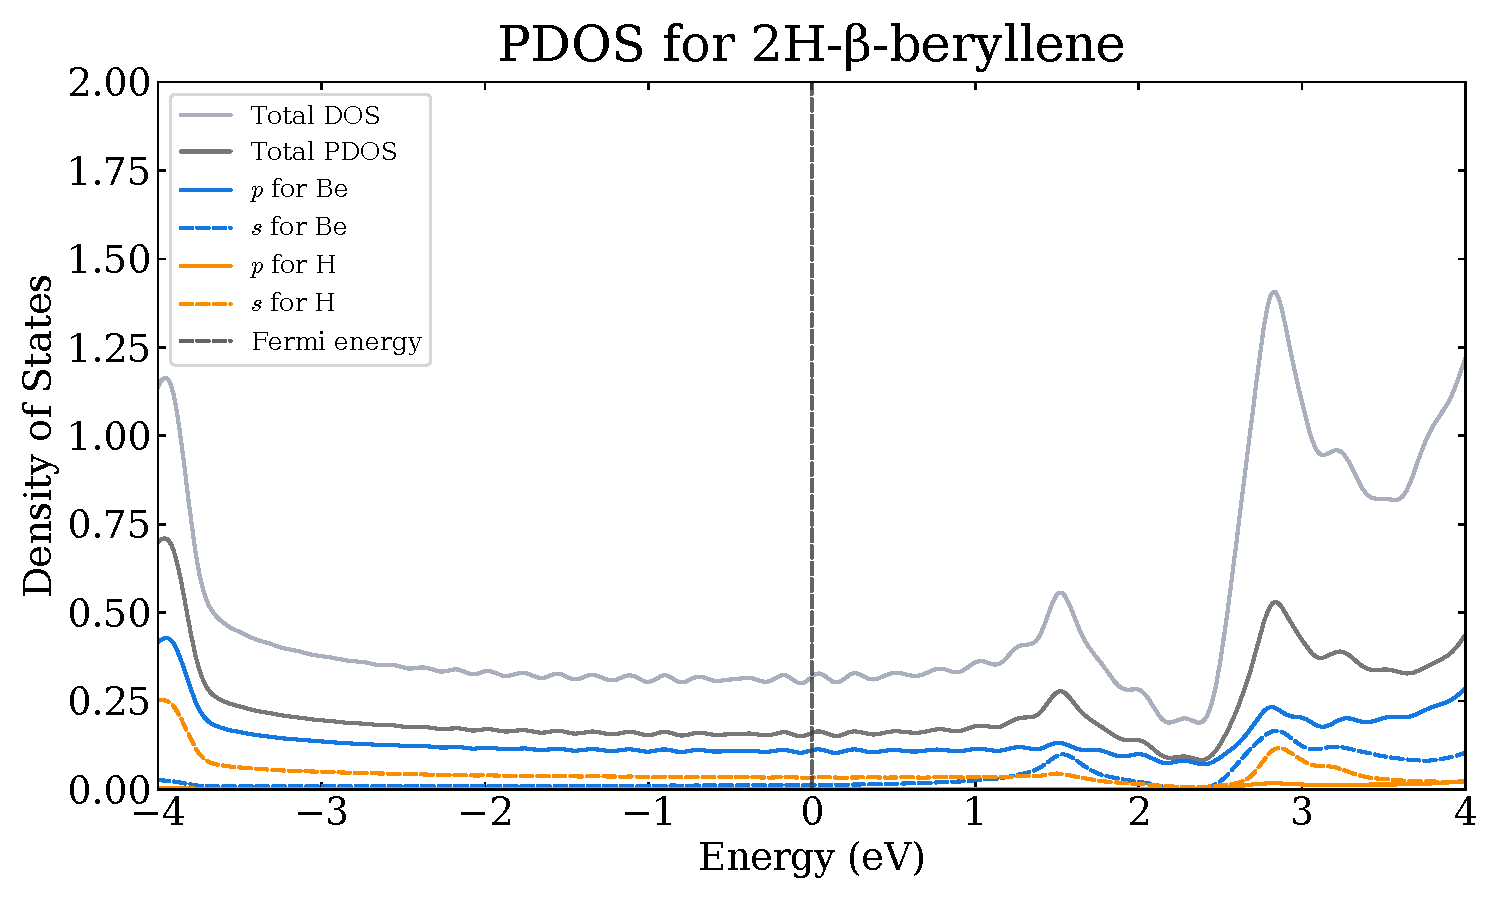
\includegraphics[width=0.40\linewidth]{figures_proj3/pdos_2H-beta-beryllene_thesis.pdf}}
\end{tabular}
\caption{Total and projected densities of states for pristine and hydrogen-functionalized beryllene structures.
Upper left: total density of states.
Upper right: projected density of states of 2H-$\alpha$-beryllene.
Lower left: projected density of states of 1H-$\beta$-beryllene.
Lower right: projected density of states of 2H-$\beta$-beryllene.}
\label{fig:proj3_dos_hydrogenated}
\end{figure}

\subsection{Topological properties}
\label{3_topological_properties}

Previous studies reported non-trivial topology in $\alpha$-beryllene,
whereas $\beta$-beryllene was classified as topologically trivial~\cite{li2023coexistence}.
$\alpha$-beryllene,
$\beta$-beryllene,
trilayer cubic beryllene,
2H-$\alpha$-beryllene,
and 2H-$\beta$-beryllene have inversion symmetry.
We therefore verify their topological character using the $\mathbb{Z}_2$ index calculated from the parity eigenvalues of the spin-orbit-coupled states at the time-reversal invariant momenta.
1H-$\beta$-beryllene has no inversion symmetry,
so its $\mathbb{Z}_2$ index is obtained from the evolution of the Wannier charge centres~\cite{soluyanov2011computing,gresch2017z2pack}.

The calculation settings are described in section~\ref{3_methods}.
The $\mathbb{Z}_2$ index $\nu$ follows from the parity products $\delta_i$ of the lowest $N$ spinor bands at the four time-reversal invariant momenta $\Gamma$,
$\mathrm{X}$,
$\mathrm{Y}$,
and $\mathrm{M}$,
according to equations~\eqref{eq:proj3_parity_product} and~\eqref{eq:proj3_z2_index}.
Here, $N$ is the number of spinor bands in the selected subspace.

Except for 2H-$\alpha$-beryllene,
the structures considered here are metallic,
so the lowest $N$ bands are not completely filled.
In this case,
$\nu$ is defined for the subspace of the lowest $N$ bands only if this subspace is separated from band $N+1$ by a direct gap,
$E_{N+1}(\vec{k}\,)-E_{N}(\vec{k}\,)>0$,
at every $\vec{k}$ in the Brillouin zone.
The index then describes a band inversion within this subspace,
while the states at the Fermi level remain metallic.
We therefore determine the minimum of this direct gap over the Brillouin zone,
as described in section~\ref{3_methods}.
As these gaps are sampled on a finite mesh and the analysis assumes time-reversal symmetry,
the resulting $\mathbb{Z}_2$ indices are conditional screening results.

The calculated parity eigenvalues,
parity products,
$\mathbb{Z}_2$ indices,
and minimum direct gaps are listed in table~\ref{tab:proj3_topological_parity}.
For $\alpha$-beryllene,
$\beta$-beryllene,
and 2H-$\alpha$-beryllene,
the $\mathrm{X}$,
$\mathrm{Y}$,
and $\mathrm{M}$ points correspond to the three $\mathrm{M}$ points of the hexagonal Brillouin zone,
which are equivalent by symmetry.
The Fu--Kane product therefore reduces to
$(-1)^{\nu}=\delta_{\Gamma}(\delta_{\mathrm{M}})^3=\delta_{\Gamma}\delta_{\mathrm{M}}$.
For trilayer cubic beryllene,
the $\mathrm{X}$ and $\mathrm{Y}$ points are the two equivalent $\mathrm{X}$ points of the square Brillouin zone,
which contribute as $(\delta_{\mathrm{X}})^2$,
and the product reduces to
$(-1)^{\nu}=\delta_{\Gamma}\delta_{\mathrm{M}}(\delta_{\mathrm{X}})^2=\delta_{\Gamma}\delta_{\mathrm{M}}$.
For 2H-$\beta$-beryllene,
the four time-reversal invariant momenta are not all equivalent,
and the parity products at all four points are used.

\begin{table}[!htbp]
\centering
\rowcolors{2}{gray!15}{white}
\setlength{\tabcolsep}{8pt}
\begin{adjustbox}{max width=1.0\linewidth,center}
\begin{tabular}{ccccccccc}
\hline
\rowcolor{gray!25}
structure
& $N$
& $\Gamma$
& $\mathrm{X}$
& $\mathrm{Y}$
& $\mathrm{M}$
& product
& $\nu$
& min. direct gap \\
\hline
$\alpha$-beryllene
& 2
& $+$
& $-$
& $-$
& $-$
& $-1$
& 1
& \qty{1.13}{\milli\electronvolt} \\
$\beta$-beryllene
& 4
& $+, -$
& $+, -$
& $+, -$
& $+, -$
& $+1$
& 0
& \qty{0.898}{\milli\electronvolt} \\
trilayer cubic beryllene
& 6
& $+, -, +$
& $+, -, +$
& $+, -, +$
& $-, -, +$
& $-1$
& 1
& \qty{0.735}{\milli\electronvolt} \\
2H-$\alpha$-beryllene
& 4
& $+, -$
& $-, +$
& $-, +$
& $-, +$
& $+1$
& 0
& \qty{4.92}{\electronvolt} \\
2H-$\beta$-beryllene
& 6
& $+, -, +$
& $-, +, +$
& $+, -, -$
& $-, +, -$
& $+1$
& 0
& \qty{0.177}{\electronvolt} \\
1H-$\beta$-beryllene
& 4 / 6
& --
& --
& --
& --
& --
& 0 / 0
& 0.929 / \qty{0.415}{\electronvolt} \\
\hline
\end{tabular}
\end{adjustbox}
\caption{Parity eigenvalues of the Kramers pairs of the lowest $N$ spinor bands at the time-reversal invariant momenta,
listed from the lowest pair upward,
Fu--Kane products,
$\mathbb{Z}_2$ indices,
and minimum direct gaps $E_{N+1}-E_{N}$ over the Brillouin zone.
For 1H-$\beta$-beryllene,
which has no inversion symmetry,
the $\mathbb{Z}_2$ indices of the lowest four and lowest six bands are obtained from the Wannier charge centres.}
\label{tab:proj3_topological_parity}
\end{table}

For $\alpha$-beryllene,
the single Kramers pair is even at the $\Gamma$ point and odd at the three zone-boundary points.
The Fu--Kane product is therefore $(-1)^{\nu}=-1$,
which gives $\nu=1$ and confirms the non-trivial topology previously reported for this phase.
These two bands are separated from band 3 at every sampled wave vector.
The smallest direct gap is the spin-orbit gap of \qty{1.13}{\milli\electronvolt} at the Dirac point at $\mathrm{K}$,
approximately \qty{2.7}{\electronvolt} above the Fermi level.
For $\beta$-beryllene,
the Fu--Kane product is $(-1)^{\nu}=+1$,
which gives $\nu=0$ and confirms that this phase is topologically trivial.
Its smallest direct gap is the spin-orbit gap of \qty{0.898}{\milli\electronvolt} at $\mathrm{K}$.
For trilayer cubic beryllene,
the parity products again change sign between the $\Gamma$ and $\mathrm{M}$ points,
giving $(-1)^{\nu}=-1$ and $\nu=1$.
At $\mathrm{M}$,
the next Kramers pair lies only \qty{1.3}{\milli\electronvolt} above band 6,
but it has the same parity as bands 5 and 6,
so the order of these two pairs does not change $\nu$.
The smallest direct gap of \qty{0.735}{\milli\electronvolt} occurs at a spin-orbit-gapped crossing on the $\Gamma$--$\mathrm{M}$ line.
Therefore,
trilayer cubic beryllene is also a non-trivial $\mathbb{Z}_2$ topological phase,
in the same conditional sense as $\alpha$-beryllene.

Both $\alpha$-beryllene and trilayer cubic beryllene are metallic at the neutral Fermi level.
Their non-trivial subspaces are isolated only by spin-orbit gaps of approximately \qty{1}{\milli\electronvolt},
located \qtyrange{1.2}{2.7}{\electronvolt} above the Fermi level.
The non-trivial index therefore characterizes a band inversion rather than a quantum spin Hall insulating state.
Gaps of this size are also far below the accuracy of the band ordering in semilocal density functional theory,
so this result may be sensitive to the exchange-correlation functional.
The convergence of these meV-scale gaps with respect to the plane-wave cutoff and the self-consistent k-point mesh has not been tested separately from the total-energy convergence.

Hydrogen functionalization gives trivial $\mathbb{Z}_2$ indices in all three structures.
2H-$\alpha$-beryllene is the only insulator among the structures considered,
so its index $\nu=0$ classifies all occupied bands.
For 2H-$\beta$-beryllene,
$\nu=0$,
and the smallest direct gap of \qty{0.177}{\electronvolt} occurs near $\mathrm{M}$.
1H-$\beta$-beryllene has five valence electrons per unit cell,
so its Fermi level lies within the half-filled fifth and sixth bands.
Its lowest four and lowest six bands are separated from the next bands by minimum direct gaps of \qty{0.929}{\electronvolt} and \qty{0.415}{\electronvolt},
respectively.
The Wannier charge centres give $\nu=0$ for both subspaces.

The parity eigenvalues at the four time-reversal invariant momenta are unchanged when the HSE06 hybrid functional is used without spin-orbit coupling.
The corresponding parity products of the five centrosymmetric structures are therefore also unchanged.
This check tests the band order at the time-reversal invariant momenta.
The isolation of the corresponding subspaces throughout the Brillouin zone with HSE06 and spin-orbit coupling is a separate test.
The converged spin-orbit-coupled states are non-magnetic,
with a magnetization density below $3\times10^{-7}~\mu_{\mathrm{B}}\,\text{\AA}^{-3}$.
Spin-polarized calculations started from ferromagnetic and antiferromagnetic configurations all converge to the non-magnetic state.
These results support the time-reversal symmetry assumed in the analysis.
For the PBE structures used in the \texttt{Quantum ESPRESSO} calculations,
the parity eigenvalues of the centrosymmetric structures and the Wilson loops give the same $\nu$ as in table~\ref{tab:proj3_topological_parity} for trilayer cubic beryllene,
2H-$\alpha$-beryllene,
2H-$\beta$-beryllene,
and 1H-$\beta$-beryllene.
In trilayer cubic beryllene,
the Wannier charge centres switch partners once along the Wilson loop.
The band structures with the lowest-$N$ subspaces are shown in figures~\ref{fig:proj3_topology_bands_pristine} and~\ref{fig:proj3_topology_bands_hydrogenated}.
The direct-gap maps,
the refinement of the smallest gaps,
and the Wannier charge centres of 1H-$\beta$-beryllene are shown in figures~\ref{fig:proj3_direct_gap_pristine}--\ref{fig:proj3_wcc},
and the HSE06 parities are listed in table~\ref{tab:proj3_hse_parity} in section~\ref{3_supplementary}.

\begin{figure}[!htbp]
\centering
    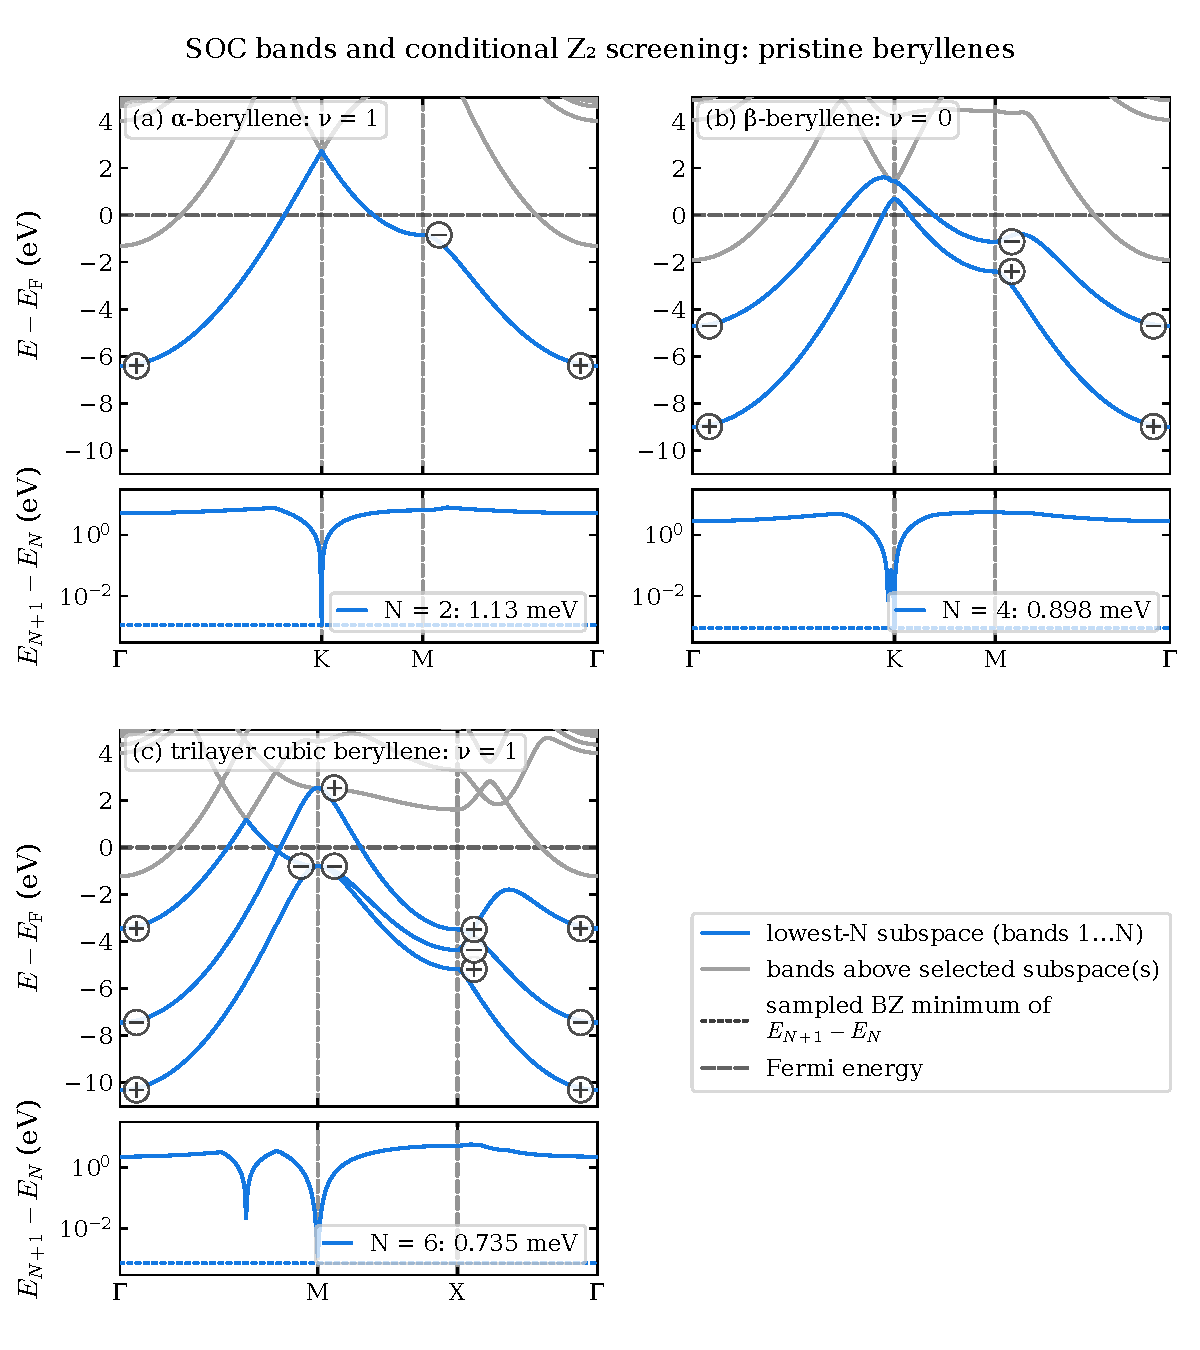
\includegraphics[width=0.80\linewidth]{figures_proj3/topology_bands_pristine_thesis.pdf}
\caption{Spin-orbit-coupled band structures of $\alpha$-beryllene,
$\beta$-beryllene,
and trilayer cubic beryllene.
The lowest $N$ bands are shown in blue,
and the parities of their Kramers pairs are marked at the time-reversal invariant momenta on the path,
where pairs within \qty{0.45}{\electronvolt} of each other share one marker and are listed from the lowest pair upward.
Below each band structure,
the direct gap $E_{N+1}-E_{N}$ along the path is shown on a logarithmic scale,
together with its minimum over the Brillouin zone.}
\label{fig:proj3_topology_bands_pristine}
\end{figure}

\begin{figure}[!htbp]
\centering
    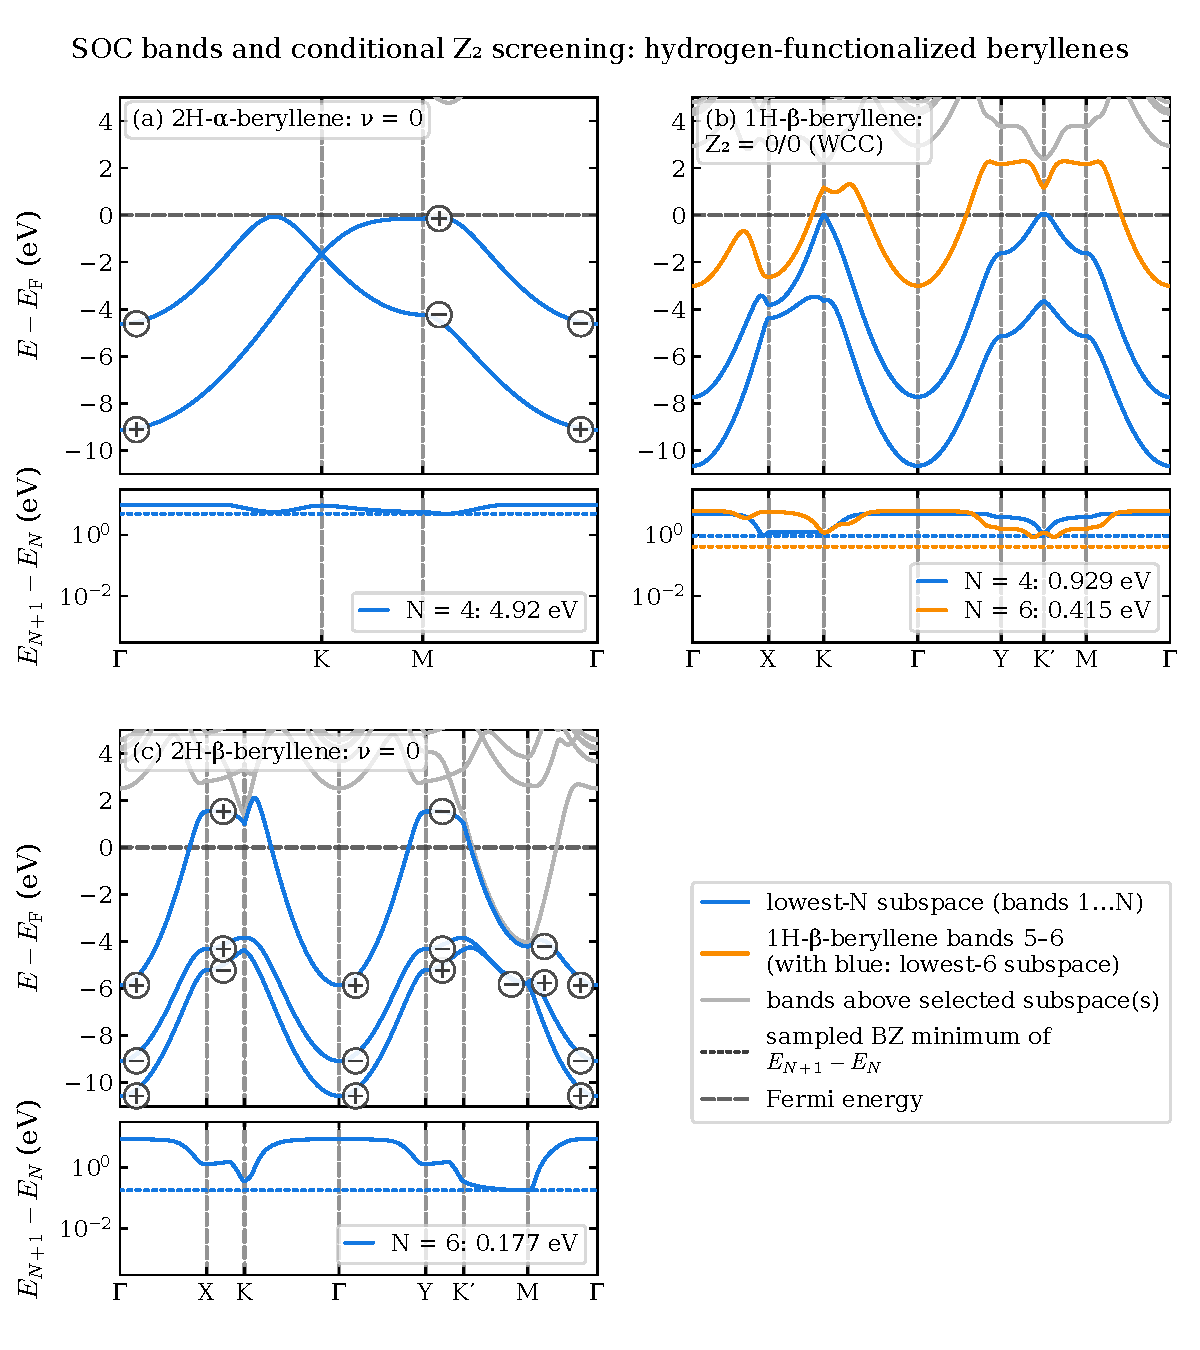
\includegraphics[width=0.80\linewidth]{figures_proj3/topology_bands_hydrogenated_thesis.pdf}
\caption{Spin-orbit-coupled band structures of 2H-$\alpha$-beryllene,
1H-$\beta$-beryllene,
and 2H-$\beta$-beryllene,
shown as in figure~\ref{fig:proj3_topology_bands_pristine}.
For 1H-$\beta$-beryllene,
bands 1--4 are shown in blue and bands 5 and 6 in orange,
corresponding to the lowest-four and lowest-six subspaces.
For 1H-$\beta$-beryllene and 2H-$\beta$-beryllene,
the path is the same as in figure~\ref{fig:proj3_band_structures_cubic_hydrogenated}.}
\label{fig:proj3_topology_bands_hydrogenated}
\end{figure}

\subsection{Electron-phonon coupling and superconductivity}
\label{3_superconductivity}

We next examine the electron-phonon coupling of the metallic trilayer cubic beryllene,
2H-$\beta$-beryllene,
and 1H-$\beta$-beryllene.
The main superconducting characteristics are listed in table~\ref{tab:proj3_superconductivity} and presented in figure~\ref{fig:proj3_superconducting_gap}.
For trilayer cubic beryllene,
the analysis gives $\lambda=0.46$,
Allen--Dynes $T_\mathrm{c}^{\mathrm{AD}}=\qty{2.0}{\kelvin}$ for $\mu^*=0.13$,
and isotropic Migdal--Eliashberg $T_\mathrm{c}^{\mathrm{iso}}=\qty{3.7}{\kelvin}$.
Trilayer cubic beryllene is therefore predicted to be a weak-coupling superconductor with a $T_\mathrm{c}$ of a few kelvin.
The electron-phonon coupling strength $\lambda$ in the case of 2H-$\beta$-beryllene is 1.40,
and the Allen--Dynes superconducting transition temperature is $T_\mathrm{c}^{\mathrm{AD}}=\qty{21.9}{\kelvin}$ for $\mu^*=0.13$.
The solution of the isotropic Migdal--Eliashberg equations gives a larger $T_\mathrm{c}^{\mathrm{iso}}$ of \qty{28.3}{\kelvin},
with $2\Delta_0/\kB T_\mathrm{c}=4.28$,
which is above the Bardeen--Cooper--Schrieffer value of 3.53~\cite{bardeen1957theory},
as shown in figure~\ref{fig:proj3_superconducting_gap}(c).
Therefore, 2H-$\beta$-beryllene is predicted to be a strong-coupling superconductor with the highest $T_\mathrm{c}$ among all cases examined.
In the case of the anisotropic solution,
the superconducting gap of 2H-$\beta$-beryllene approaches a finite value at \qtyrange{29}{31}{\kelvin},
while at \qty{32}{\kelvin} and above,
it exponentially tends to zero,
as shown in figures~\ref{fig:proj3_superconducting_gap}(c) and~(d).
Thus, the anisotropic transition temperature $T_\mathrm{c}$ falls into the range from \qty{31}{\kelvin} to \qty{32}{\kelvin} and is estimated to be \qty{31.7}{\kelvin}.
These electron-phonon calculations use the structure relaxed with the D3 dispersion correction,
whose lattice constant is \qty{2.4}{\percent} smaller than the PBE value in table~\ref{tab:proj3_hydrogenated_structural_parameters}.
On the coarse $12 \times 12 \times 1$ q-point mesh,
all phonon frequencies of this structure are real,
except for an imaginary value of $0.24\mathrm{i}$~\si{\tera\hertz} at $\Gamma$.
At the mesh point closest to the soft-mode wave vector of section~\ref{3_dynamical_stability_and_phonon_dispersion},
the lowest frequency is \qty{5.9}{\tera\hertz}.
The soft mode of the PBE structure is therefore absent from these electron-phonon calculations.
For 1H-$\beta$-beryllene,
from the Allen--Dynes expression,
we obtain $T_\mathrm{c}^{\mathrm{AD}}=\qty{8.1}{\kelvin}$ for $\mu^*=0.13$.
On the other hand,
the isotropic Migdal--Eliashberg equations give a higher $T_\mathrm{c}^{\mathrm{iso}}$ of \qty{11.6}{\kelvin},
with $2\Delta_0/\kB T_\mathrm{c}=3.64$,
as shown in figure~\ref{fig:proj3_superconducting_gap}(a).
In the anisotropic solution,
the superconducting gap approaches a finite value at \qty{14.0}{\kelvin} and \qty{14.1}{\kelvin},
about \qtyrange{0.39}{0.40}{\milli\electronvolt} and \qtyrange{0.25}{0.28}{\milli\electronvolt}, respectively,
while at \qty{14.5}{\kelvin} the gap exponentially tends to zero,
as shown in figure~\ref{fig:proj3_superconducting_gap}(b).
At \qty{14.2}{\kelvin},
the temperature closest to $T_\mathrm{c}$,
the gap does not reach a plateau and does not exponentially decay during approximately 5000 iterations.
As a consequence,
$T_\mathrm{c}$ in the anisotropic case lies between \qty{14.1}{\kelvin} and \qty{14.5}{\kelvin} and can be estimated to be \qty{14.2}{\kelvin}.
Therefore, the gap anisotropy increases $T_\mathrm{c}$ by about \qtyrange{2.5}{2.9}{\kelvin} compared with the isotropic value.

\begin{table}[!htbp]
\centering
\rowcolors{2}{gray!15}{white}
\begin{adjustbox}{max width=1.0\linewidth,center}
\begin{tabular}{cccccccc}
\hline
\rowcolor{gray!25}
structure
& $\lambda$
& $\hbar\omega_\mathrm{log}$ (meV)
& $T_\mathrm{c}^{\mathrm{AD}}$ (K)
& $T_\mathrm{c}^{\mathrm{iso}}$ (K)
& $\Delta_0$ (meV)
& $2\Delta_0/\kB T_\mathrm{c}$
& $T_\mathrm{c}^{\mathrm{aniso}}$ (K) \\
\hline
trilayer cubic beryllene
& 0.46 & 36.0 & 3.7 / 2.0 / 0.9 & 3.7 & 0.57 & 3.58 & -- \\
2H-$\beta$-beryllene
& 1.40 & 19.5 & 24.2 / 21.9 / 19.6 & 28.3 & 5.23 & 4.28 & $\approx 31.7$ \\
1H-$\beta$-beryllene
& 0.61 & 40.7 & 11.4 / 8.1 / 5.4 & 11.6 & 1.83 & 3.64 & $\approx 14.2$ \\
\hline
\end{tabular}
\end{adjustbox}
\caption{Electron-phonon coupling strength $\lambda$,
logarithmic average frequency $\omega_\mathrm{log}$,
Allen--Dynes transition temperature $T_\mathrm{c}^{\mathrm{AD}}$ from equation~\eqref{allen_dynes_temperature_estimate} for $\mu^*=0.10$, 0.13, and 0.16,
isotropic Migdal--Eliashberg transition temperature $T_\mathrm{c}^{\mathrm{iso}}$ with the fitted gap amplitude $\Delta_0$ and gap ratio,
and anisotropic Migdal--Eliashberg transition temperature $T_\mathrm{c}^{\mathrm{aniso}}$.
All values are calculated on $80 \times 80 \times 1$ fine meshes with the phonon frequency thresholds given in section~\ref{3_methods},
and $\mu^*=0.13$ is used for the Migdal--Eliashberg calculations.}
\label{tab:proj3_superconductivity}
\end{table}

\begin{figure}[!htbp]
\centering
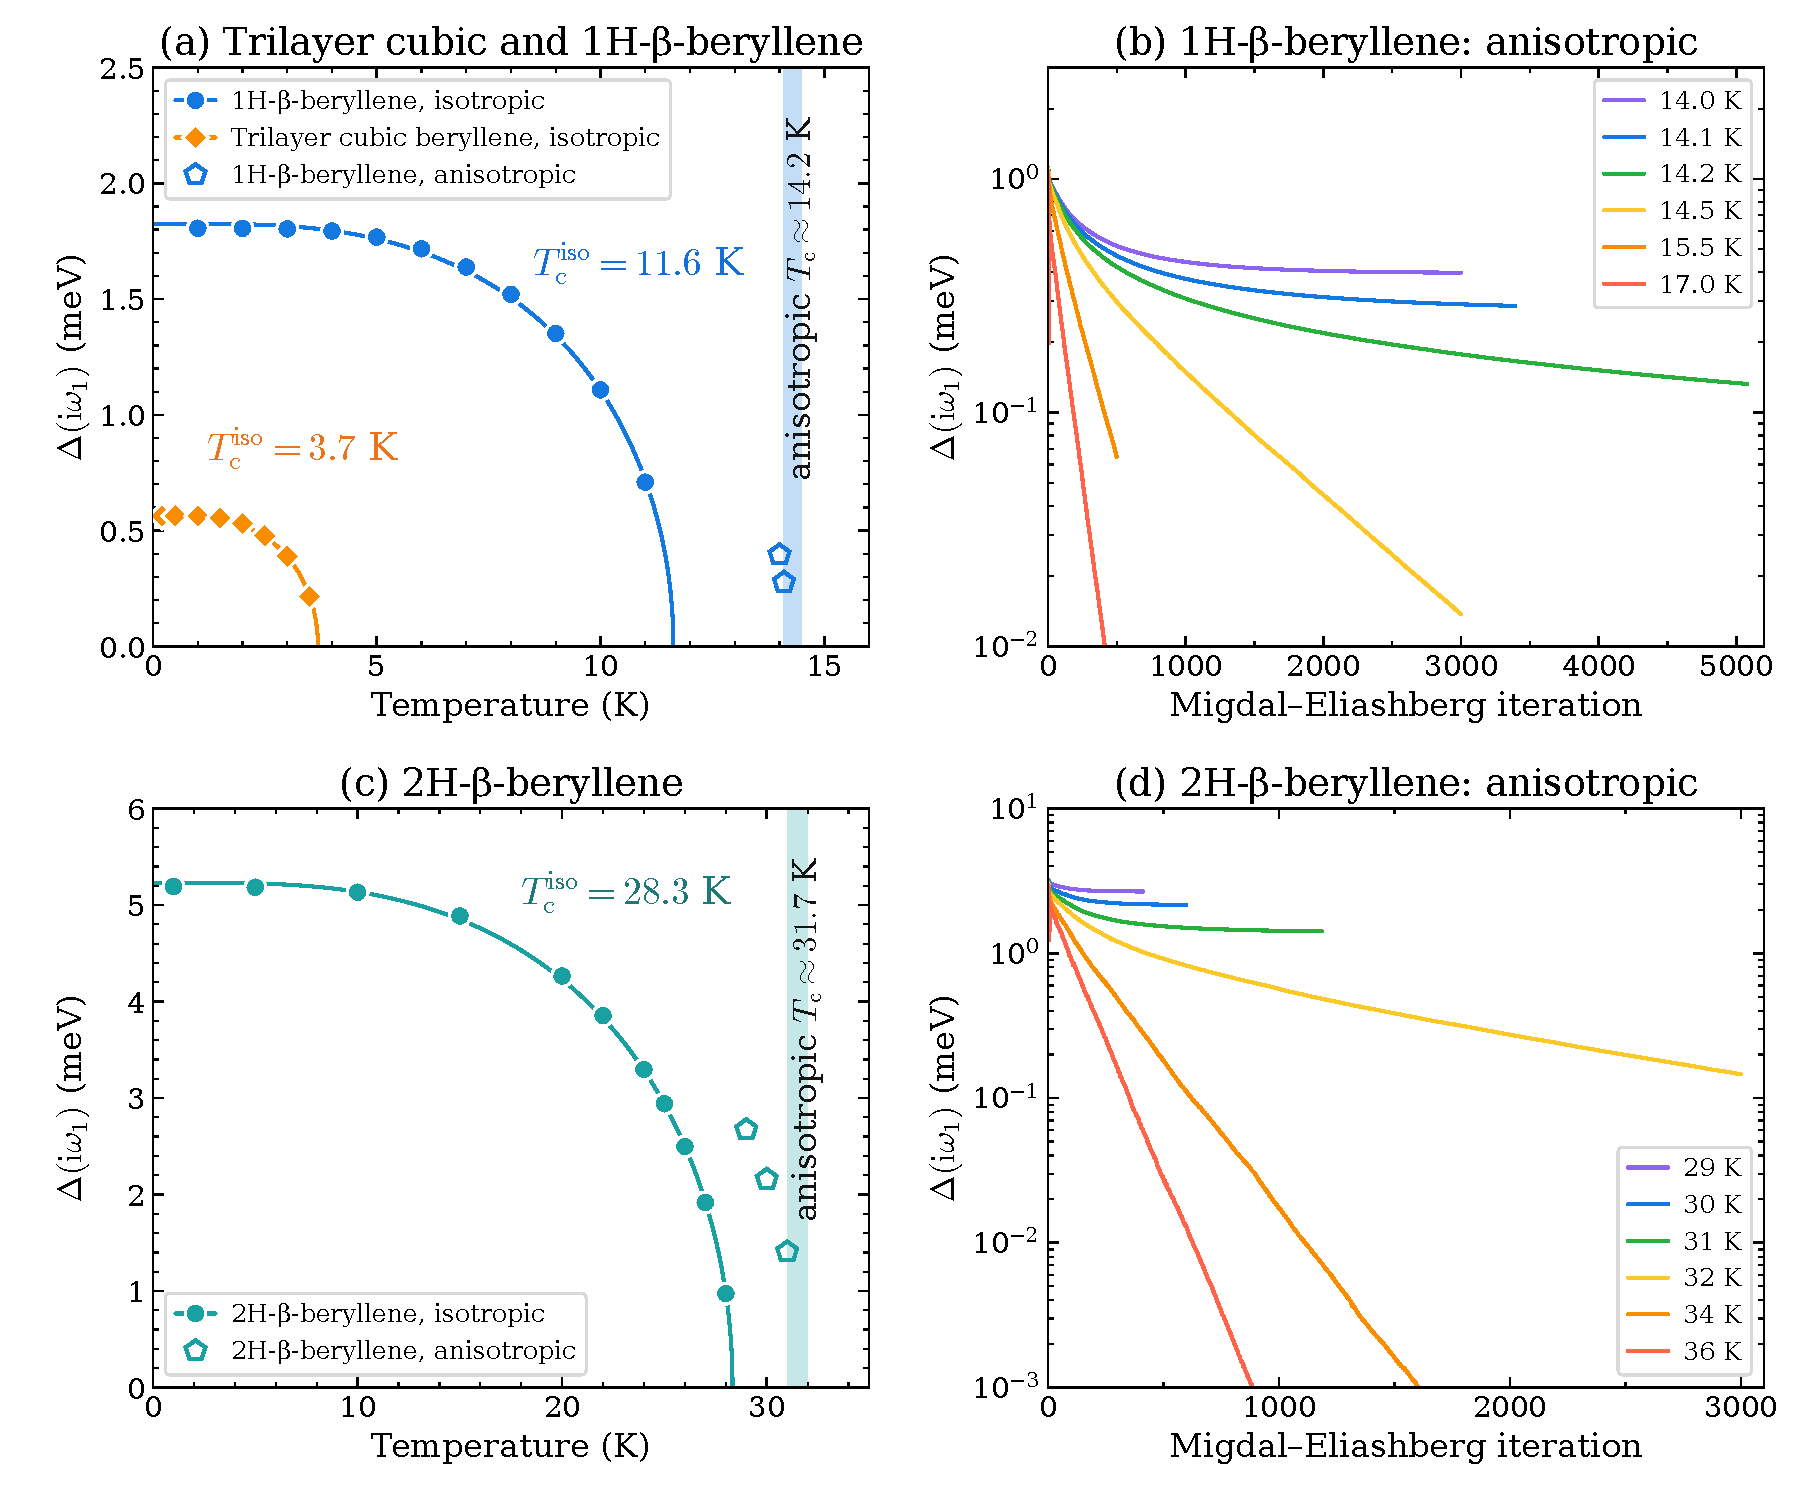
\includegraphics[width=0.80\linewidth]{figures_proj3/superconductivity/superconductivity.pdf}
\caption{Superconducting gap.
(a) Gap at the first Matsubara frequency, $\Delta(\mathrm{i}\omega_1)$, as a function of temperature,
with $\omega_1=\mathrm{\pi}\kB T/\hbar$.
Circles and squares represent the isotropic Migdal--Eliashberg solutions of 1H-$\beta$-beryllene and trilayer cubic beryllene, respectively,
while lines correspond to fits with $\Delta_0\tanh\left[1.74\left(T_\mathrm{c}/T-1\right)^{1/2}\right]$.
Open diamonds show the anisotropic gaps below $T_\mathrm{c}$,
and the shaded band marks the anisotropic $T_\mathrm{c}$.
(b) Fermi-surface-averaged $\Delta(\mathrm{i}\omega_1)$ of 1H-$\beta$-beryllene in the anisotropic Migdal--Eliashberg iterations.
(c) and (d) are analogous to (a) and (b), respectively, for 2H-$\beta$-beryllene.}
\label{fig:proj3_superconducting_gap}
\end{figure}

\subsection{Optical properties}
\label{3_optical_properties}

We now examine the optical properties of the pristine and hydrogen-functionalized beryllene structures,
together with the bulk hcp and bulk bcc beryllium reference phases.
The dielectric function,
absorption coefficient,
refractive index,
extinction coefficient,
reflectivity,
and energy-loss spectrum are defined in chapter~\ref{cha:fundamentals_b},
especially sections~\ref{sec:from_electronic_response_to_dielectric_function} and~\ref{sec:from_dielectric_function_to_optical_properties}.
Here,
we use scalar quantities derived from the Cartesian diagonal dielectric components to compare the direction-dependent optical response of the beryllene structures.

\subsubsection{Pristine $\alpha$- and $\beta$-beryllene}
\label{3_optical_alpha_beta}

We first discuss the optical response of pristine $\alpha$-beryllene and $\beta$-beryllene,
which then provides a reference for bulk beryllium,
trilayer cubic beryllene,
and the hydrogen-functionalized structures.
The real and imaginary parts of the dielectric function for the in-plane and out-of-plane directions are shown in figure~\ref{fig:proj3_alpha_beta_dielectric}.

For $\beta$-beryllene,
the in-plane real part contains zero crossings and a low-energy interval in which its sign differs from the out-of-plane component.
On the calculated energy grid, these components have opposite signs from approximately \qtyrange{1.22}{2.21}{\electronvolt}~\cite{ghavami2024transitions}.
For $\alpha$-beryllene, the out-of-plane real part crosses zero near \qty{10.64}{\electronvolt}, where the imaginary part is comparatively small.
The sign changes and energy-loss features identify candidate energy ranges for further analysis of collective response.
Establishing propagating modes in a finite two-dimensional layer and their lifetimes belongs to that further analysis.
The numerical broadening is an input to the calculation.

\begin{figure}[!htbp]
\centering
    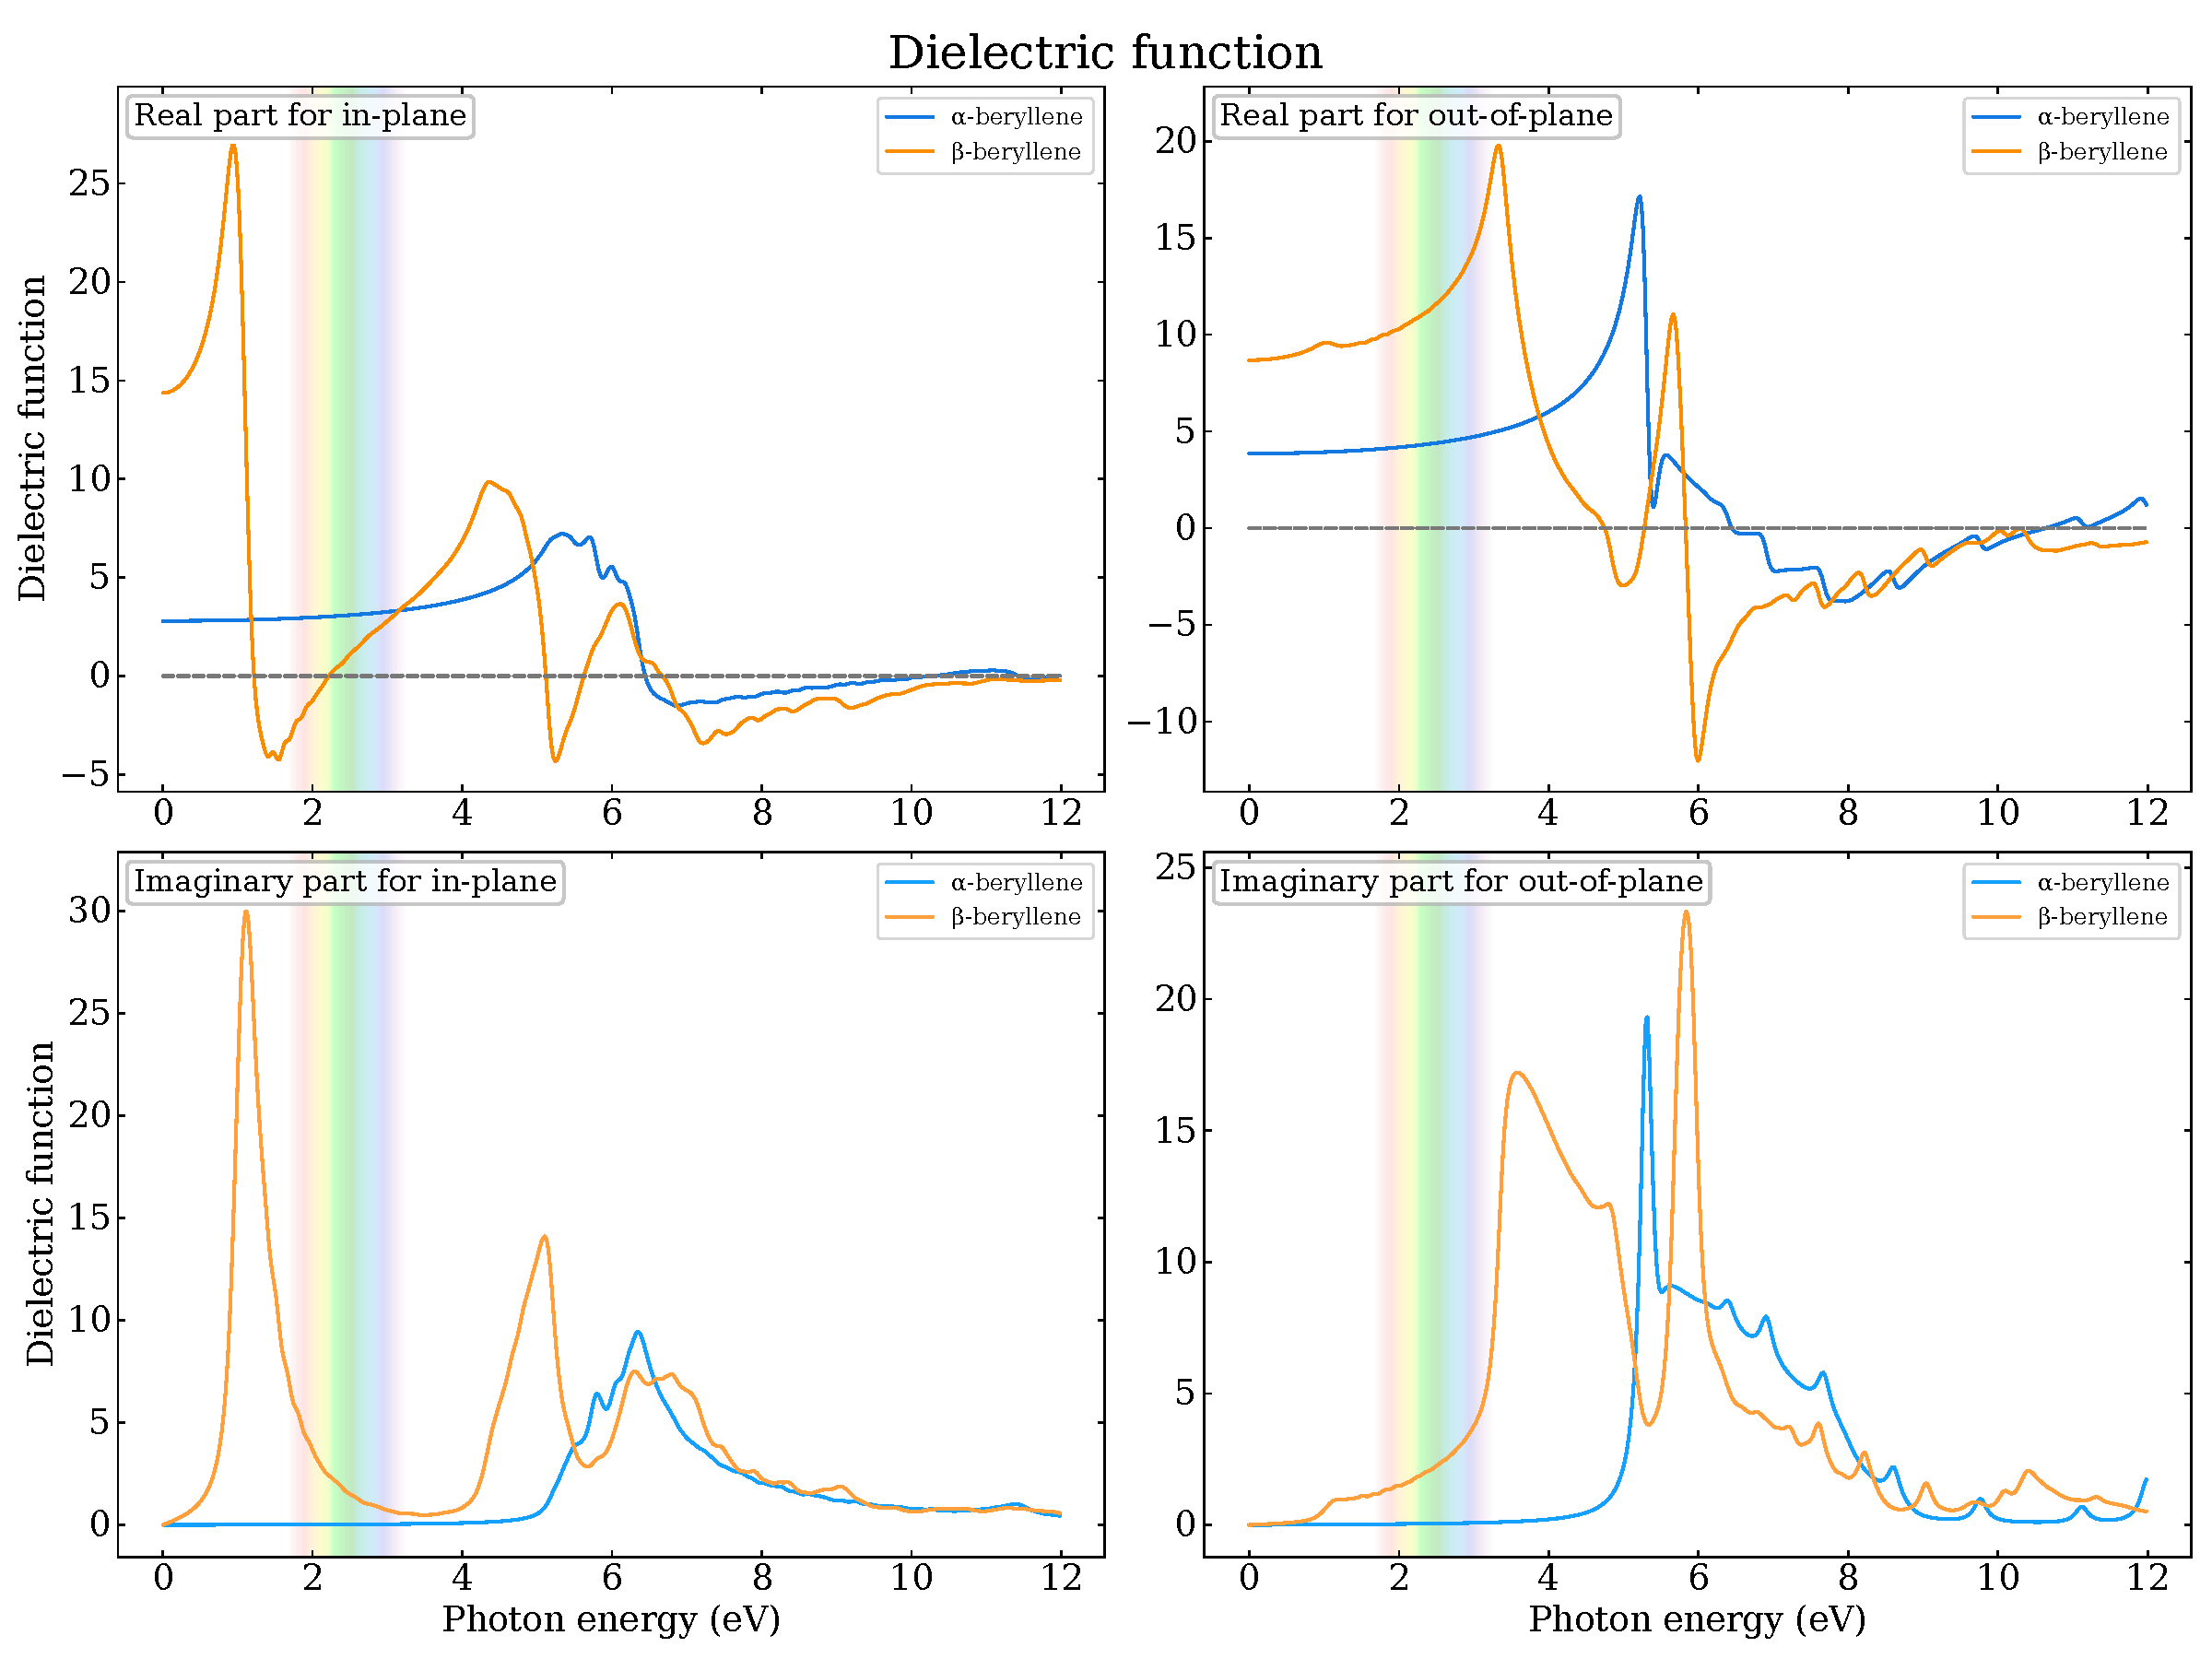
\includegraphics[width=0.80\linewidth]{figures_proj3/dielectric_alpha-beta_thesis.pdf}
\caption{Real and imaginary parts of the dielectric function for $\alpha$-beryllene and $\beta$-beryllene.
The spectra are shown for the in-plane and out-of-plane directions as functions of photon energy.
The in-plane and out-of-plane curves correspond to the $xx$ and $zz$ components, respectively.}
\label{fig:proj3_alpha_beta_dielectric}
\end{figure}

The absorption coefficient and refractive index are shown in figure~\ref{fig:proj3_alpha_beta_abs_refractive}.
The effective absorption is strongly anisotropic.
Within the \qtyrange{0}{12}{\electronvolt} window, the largest sampled coefficients for $\alpha$-beryllene are approximately
\qty{0.135}{\per\nano\metre} in $xx$ and \qty{0.175}{\per\nano\metre} in $zz$.
The corresponding $\beta$-beryllene values are approximately \qty{0.161}{\per\nano\metre} and \qty{0.242}{\per\nano\metre}.
The strongest $\beta$ out-of-plane feature occurs near \qty{5.95}{\electronvolt}.
The spectra cross at some energies, so $\beta$-beryllene absorbs more strongly only over part of the energy range.

The refractive-index spectra follow the same structural and directional contrast.
In the in-plane channel,
$\beta$-beryllene develops two pronounced enhancements in the infrared and near-ultraviolet regions,
with a minimum in the visible range.
By contrast,
$\alpha$-beryllene varies more smoothly over the same energy interval.
In the out-of-plane channel,
$\beta$-beryllene remains stronger than $\alpha$-beryllene over the infrared to near-ultraviolet range.
The first downward $n=1$ crossings occur near \qty{7.42}{\electronvolt} for $\alpha$ $xx$,
\qty{7.82}{\electronvolt} for $\alpha$ $zz$, \qty{7.32}{\electronvolt} for $\beta$ $xx$, and \qty{6.37}{\electronvolt} for $\beta$ $zz$.
The $\alpha$ out-of-plane index rises above one again near \qty{11.71}{\electronvolt}.
These crossings describe the dispersion of the effective optical constants, and a plasmon assignment requires the energy-loss spectrum as well.

\begin{figure}[!htbp]
\centering
    \adjustbox{valign=c}{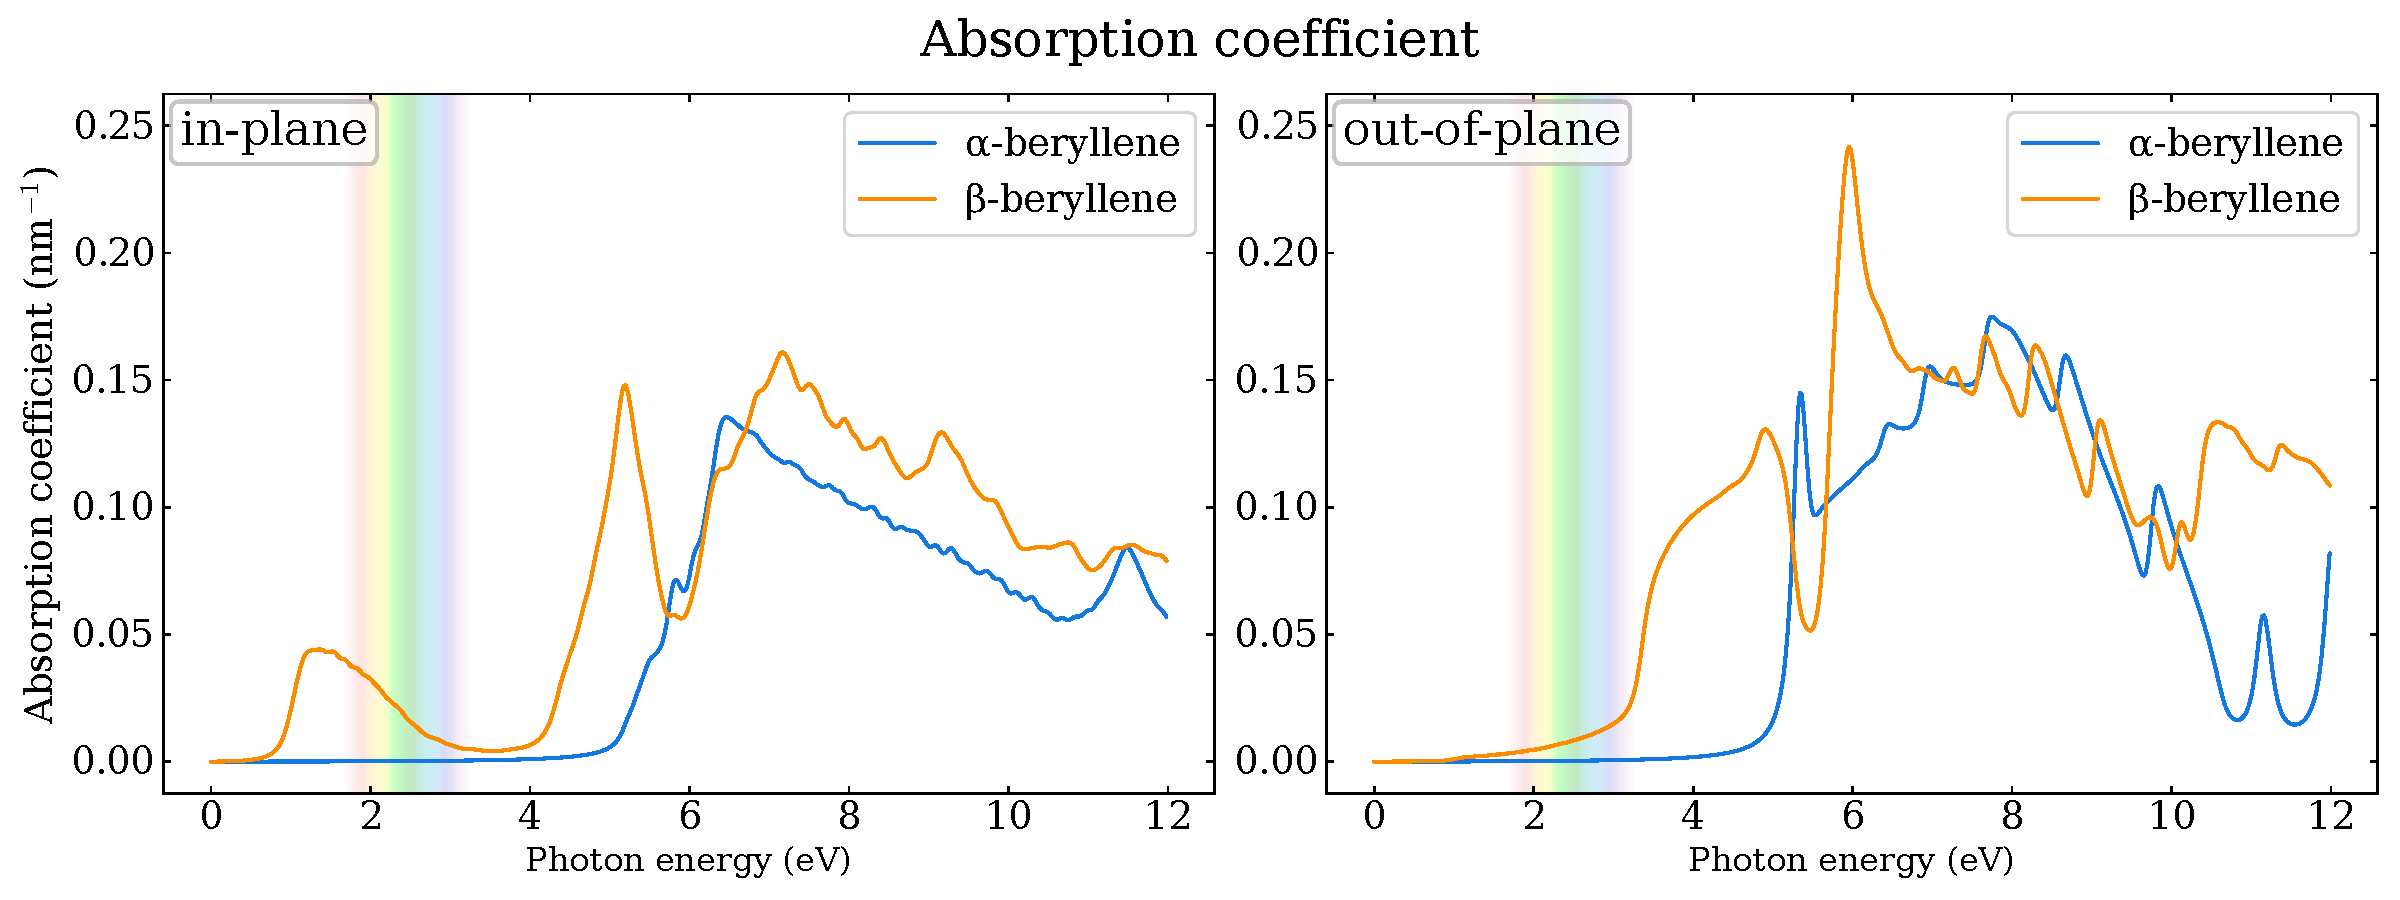
\includegraphics[width=0.80\linewidth]{figures_proj3/optics_alpha-beta_absorption_thesis.pdf}}%
    \par\nointerlineskip
    \adjustbox{valign=c}{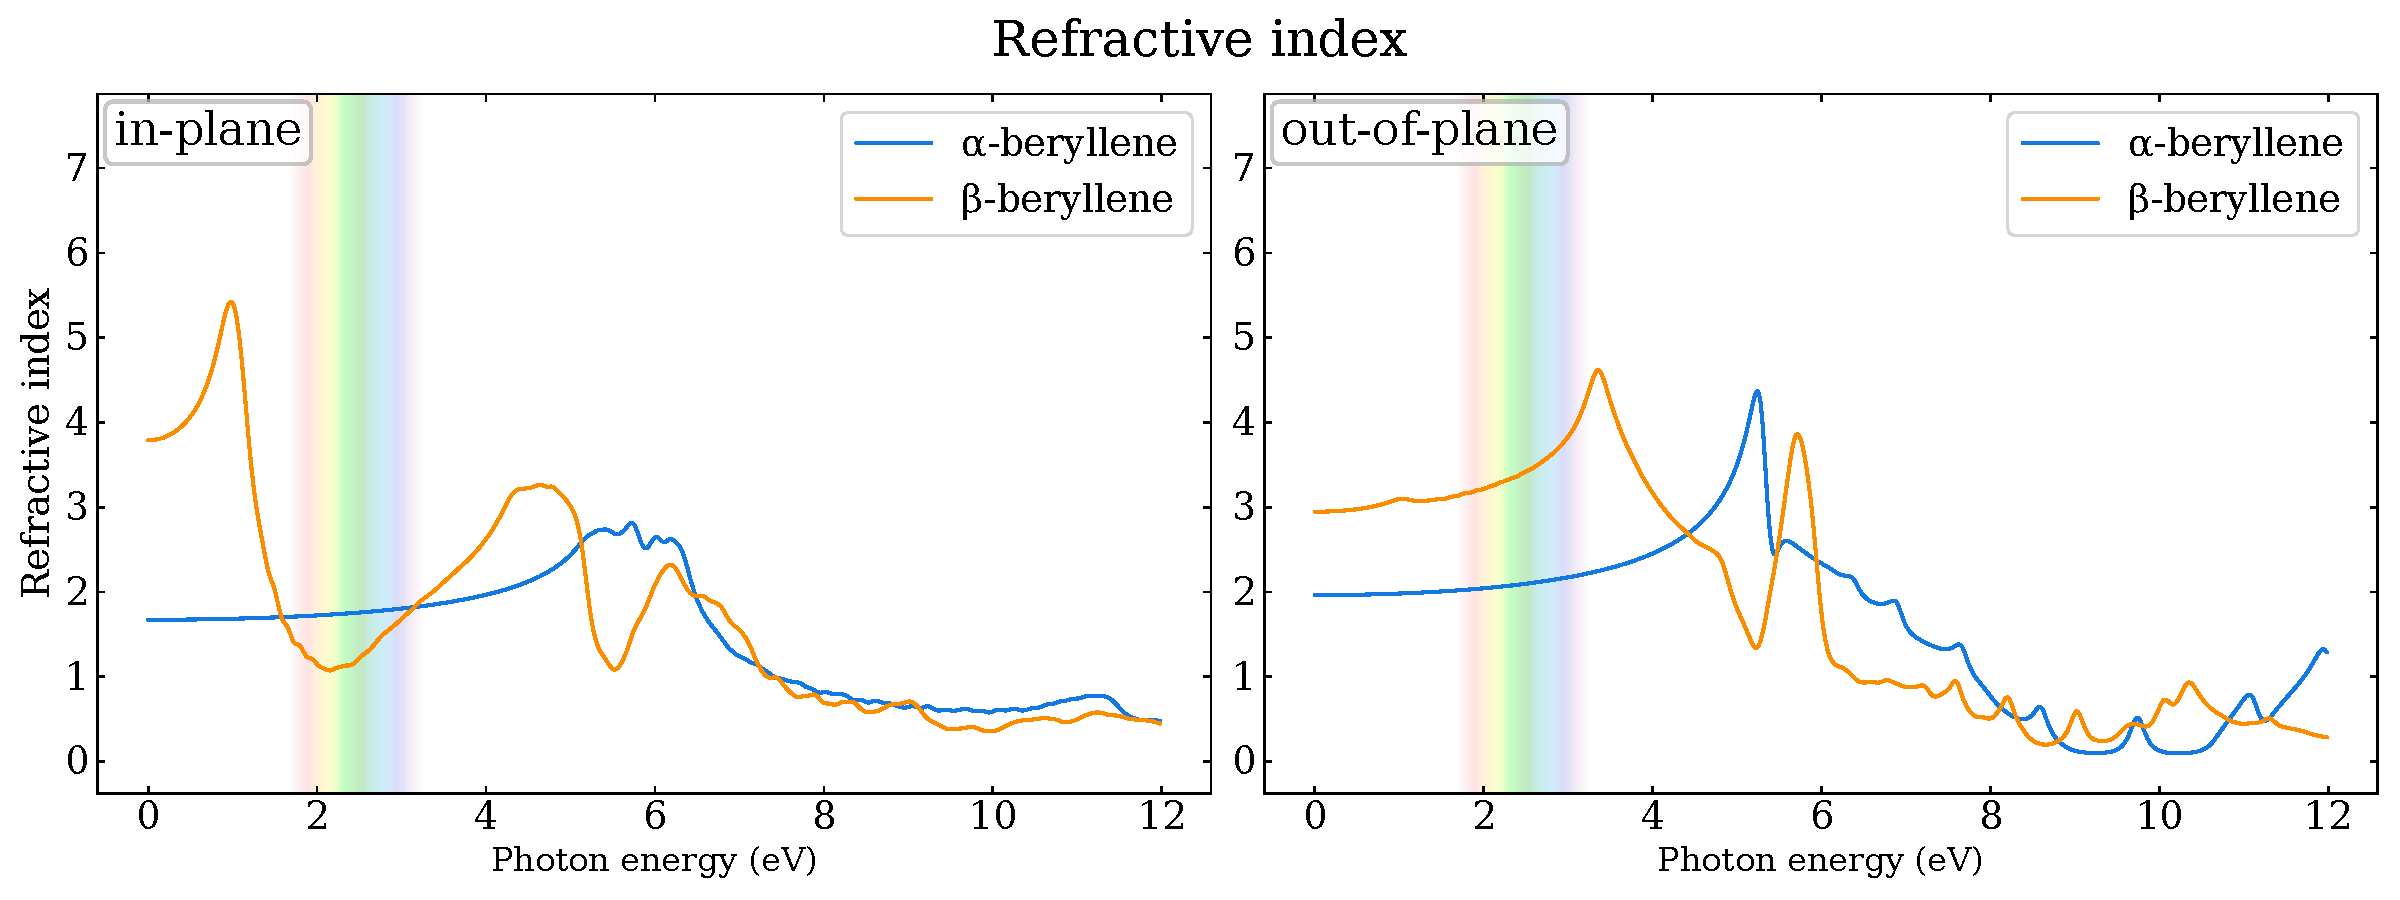
\includegraphics[width=0.80\linewidth]{figures_proj3/optics_alpha-beta_refractive_thesis.pdf}}%
\caption{Absorption coefficient and refractive index of $\alpha$-beryllene and $\beta$-beryllene.
Upper: absorption coefficient ($\mathrm{nm}^{-1}$). Lower: refractive index.
The spectra are shown for the in-plane and out-of-plane directions as functions of photon energy.
The in-plane and out-of-plane curves correspond to the $xx$ and $zz$ components, respectively.}
\label{fig:proj3_alpha_beta_abs_refractive}
\end{figure}

The extinction coefficient is shown in figure~\ref{fig:proj3_alpha_beta_extinction}.
In the in-plane channel,
$\beta$-beryllene develops strong peaks in the infrared and near-ultraviolet regions,
separated by a pronounced trough.
By contrast,
$\alpha$-beryllene again varies more smoothly.
In the out-of-plane channel,
$\beta$-beryllene develops its strongest extinction peak near \qty{5.95}{\electronvolt}, where $k\approx4.00$, followed by weaker higher-energy features.
This behaviour shows that amplitude attenuation also depends on both optical direction and crystal structure.

\begin{figure}[!htbp]
\centering
    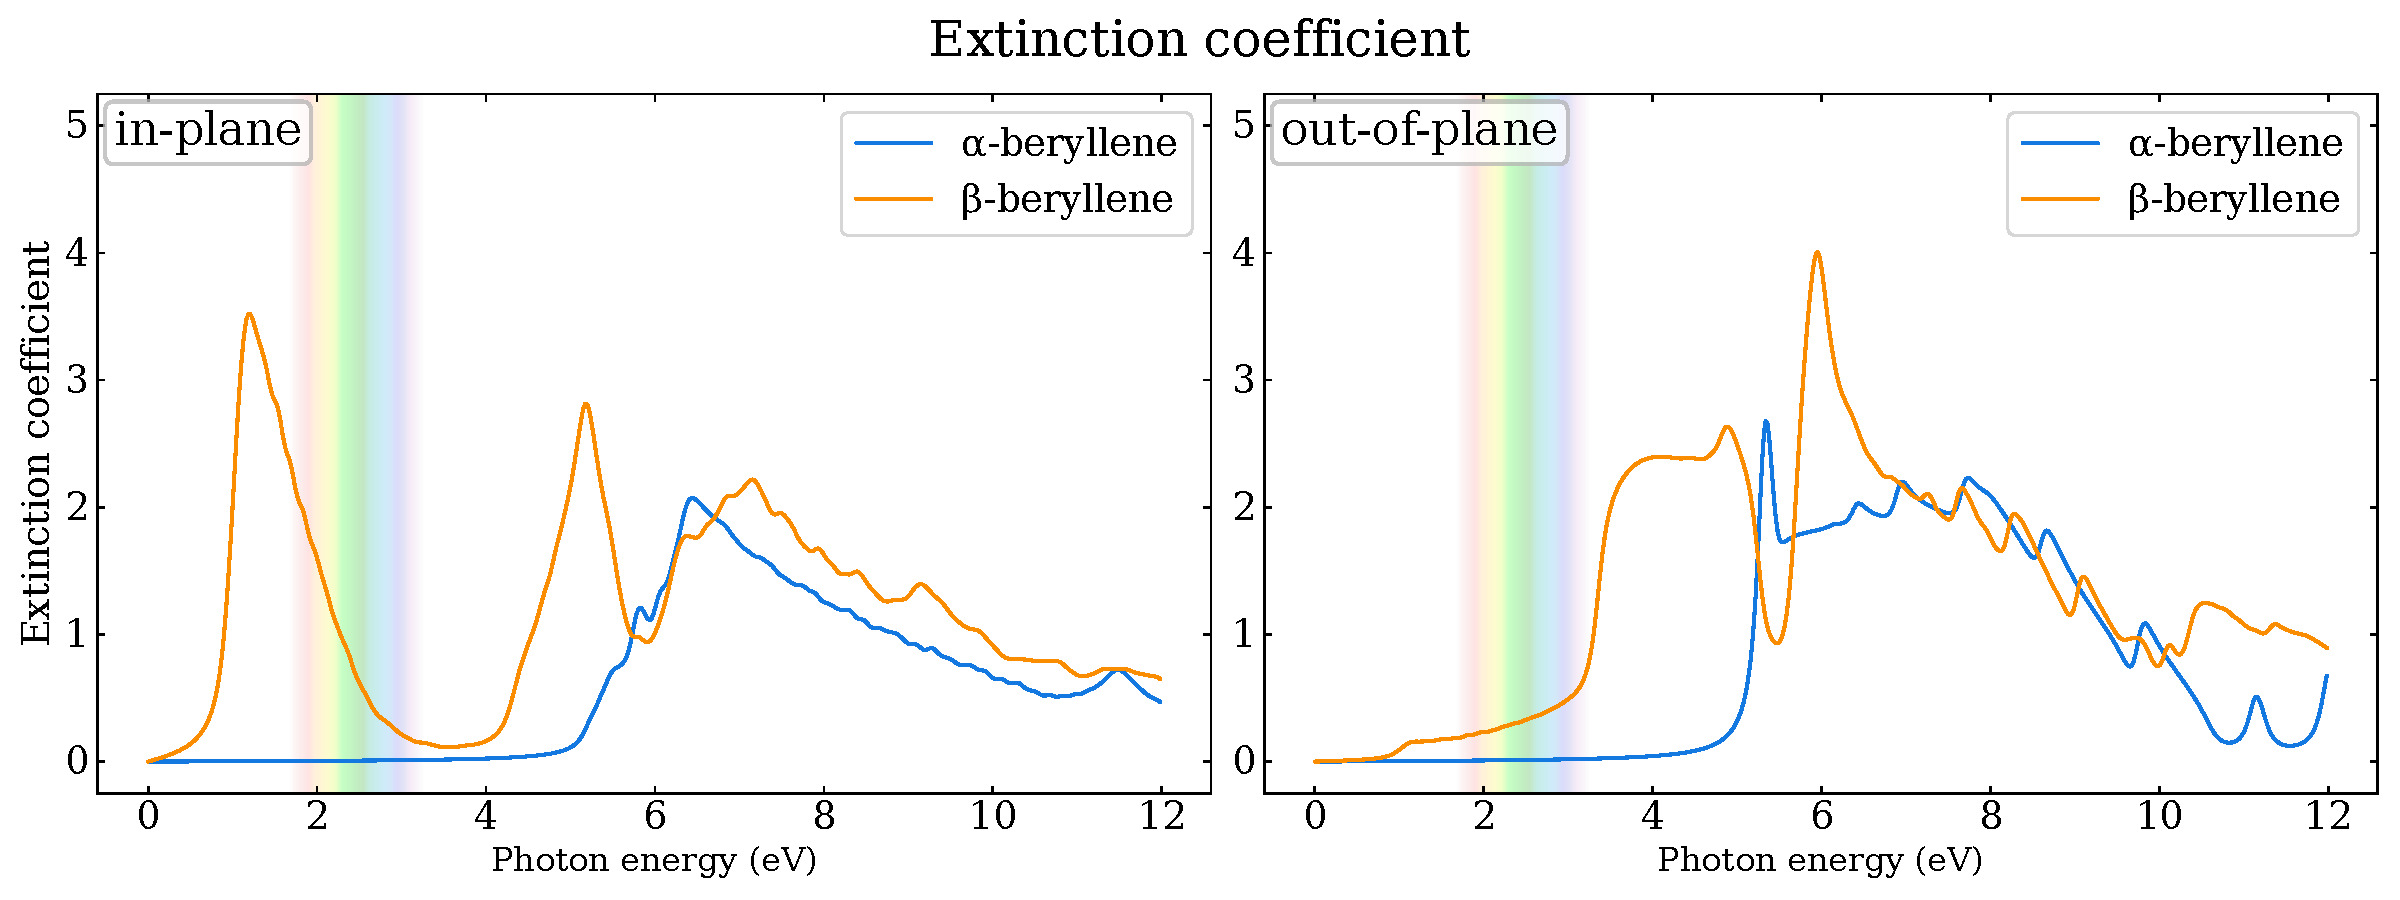
\includegraphics[width=0.80\linewidth]{figures_proj3/optics_alpha-beta_extinction_thesis.pdf}
\caption{Extinction coefficient of $\alpha$-beryllene and $\beta$-beryllene for the in-plane and out-of-plane directions as a function of photon energy.
The in-plane and out-of-plane curves correspond to the $xx$ and $zz$ components, respectively.}
\label{fig:proj3_alpha_beta_extinction}
\end{figure}

The corresponding reflectivity and energy-loss spectra,
given in figures~\ref{fig:proj3_reflectivity_alpha_beta} and~\ref{fig:proj3_energy_loss_alpha_beta} in section~\ref{3_supplementary},
show the same structural and directional contrast.
For reflectivity,
$\beta$-beryllene shows strong reflection in the low-energy and near-ultraviolet regions for in-plane polarization,
separated by a pronounced minimum.
In contrast,
$\alpha$-beryllene changes more smoothly and shows a broad intermediate-energy feature.
For out-of-plane polarization,
$\beta$-beryllene remains stronger over the low-energy range,
whereas $\alpha$-beryllene shows pronounced peaks in the ultraviolet region.

The in-plane energy-loss spectrum of $\beta$-beryllene has a visible-range local maximum of approximately 0.49
and a larger high-energy local maximum of approximately 1.34 near \qty{11.03}{\electronvolt}.
It reaches approximately 1.50 at the last available sample near \qty{11.98}{\electronvolt} while still rising.
For the out-of-plane response,
$\alpha$-beryllene has a dominant energy-loss maximum of approximately 8.88 near \qty{10.64}{\electronvolt},
substantially above the $\beta$ maximum of approximately 1.09 near \qty{9.95}{\electronvolt}.

\subsubsection{Bulk hcp, bulk bcc, and trilayer cubic beryllene}
\label{3_optical_bulk_cubic}

We next compare the optical response of bulk hcp beryllium,
bulk bcc beryllium,
and trilayer cubic beryllene.
The real and imaginary parts of the dielectric function are shown in figure~\ref{fig:proj3_bulk_cubic_dielectric}.
Bulk hcp and bulk bcc beryllium show similar behaviour and weak directional dependence.
For both bulk structures,
the real part becomes negative at \qtyrange{4.4}{4.9}{\electronvolt},
reaches a minimum at \qtyrange{5.3}{6.2}{\electronvolt},
and then rises smoothly towards zero around \qty{12}{\electronvolt}.
The imaginary part displays a broad low-energy feature up to approximately \qty{5.5}{\electronvolt},
indicating a wide range of allowed interband transitions.
It then decreases sharply around \qty{6}{\electronvolt},
coinciding with a minimum in the real part and a change in the inverse dielectric response.

For trilayer cubic beryllene,
the dielectric response is redistributed and becomes direction dependent relative to bulk bcc beryllium.
The largest imaginary dielectric features occur near \qty{3.74}{\electronvolt} in $xx$ and $yy$,
with a value of approximately 19.75,
and near \qty{2.71}{\electronvolt} in $zz$,
with a value of approximately 27.32.
The real part also develops direction-dependent sign changes.
These dielectric features do not coincide in general with absorption maxima,
which also depend on the photon energy and the non-linear relation between the dielectric function and the extinction coefficient.
Assignments to specific surface bands or transitions would require band- and matrix-element-resolved evidence.

\begin{figure}[!htbp]
\centering
    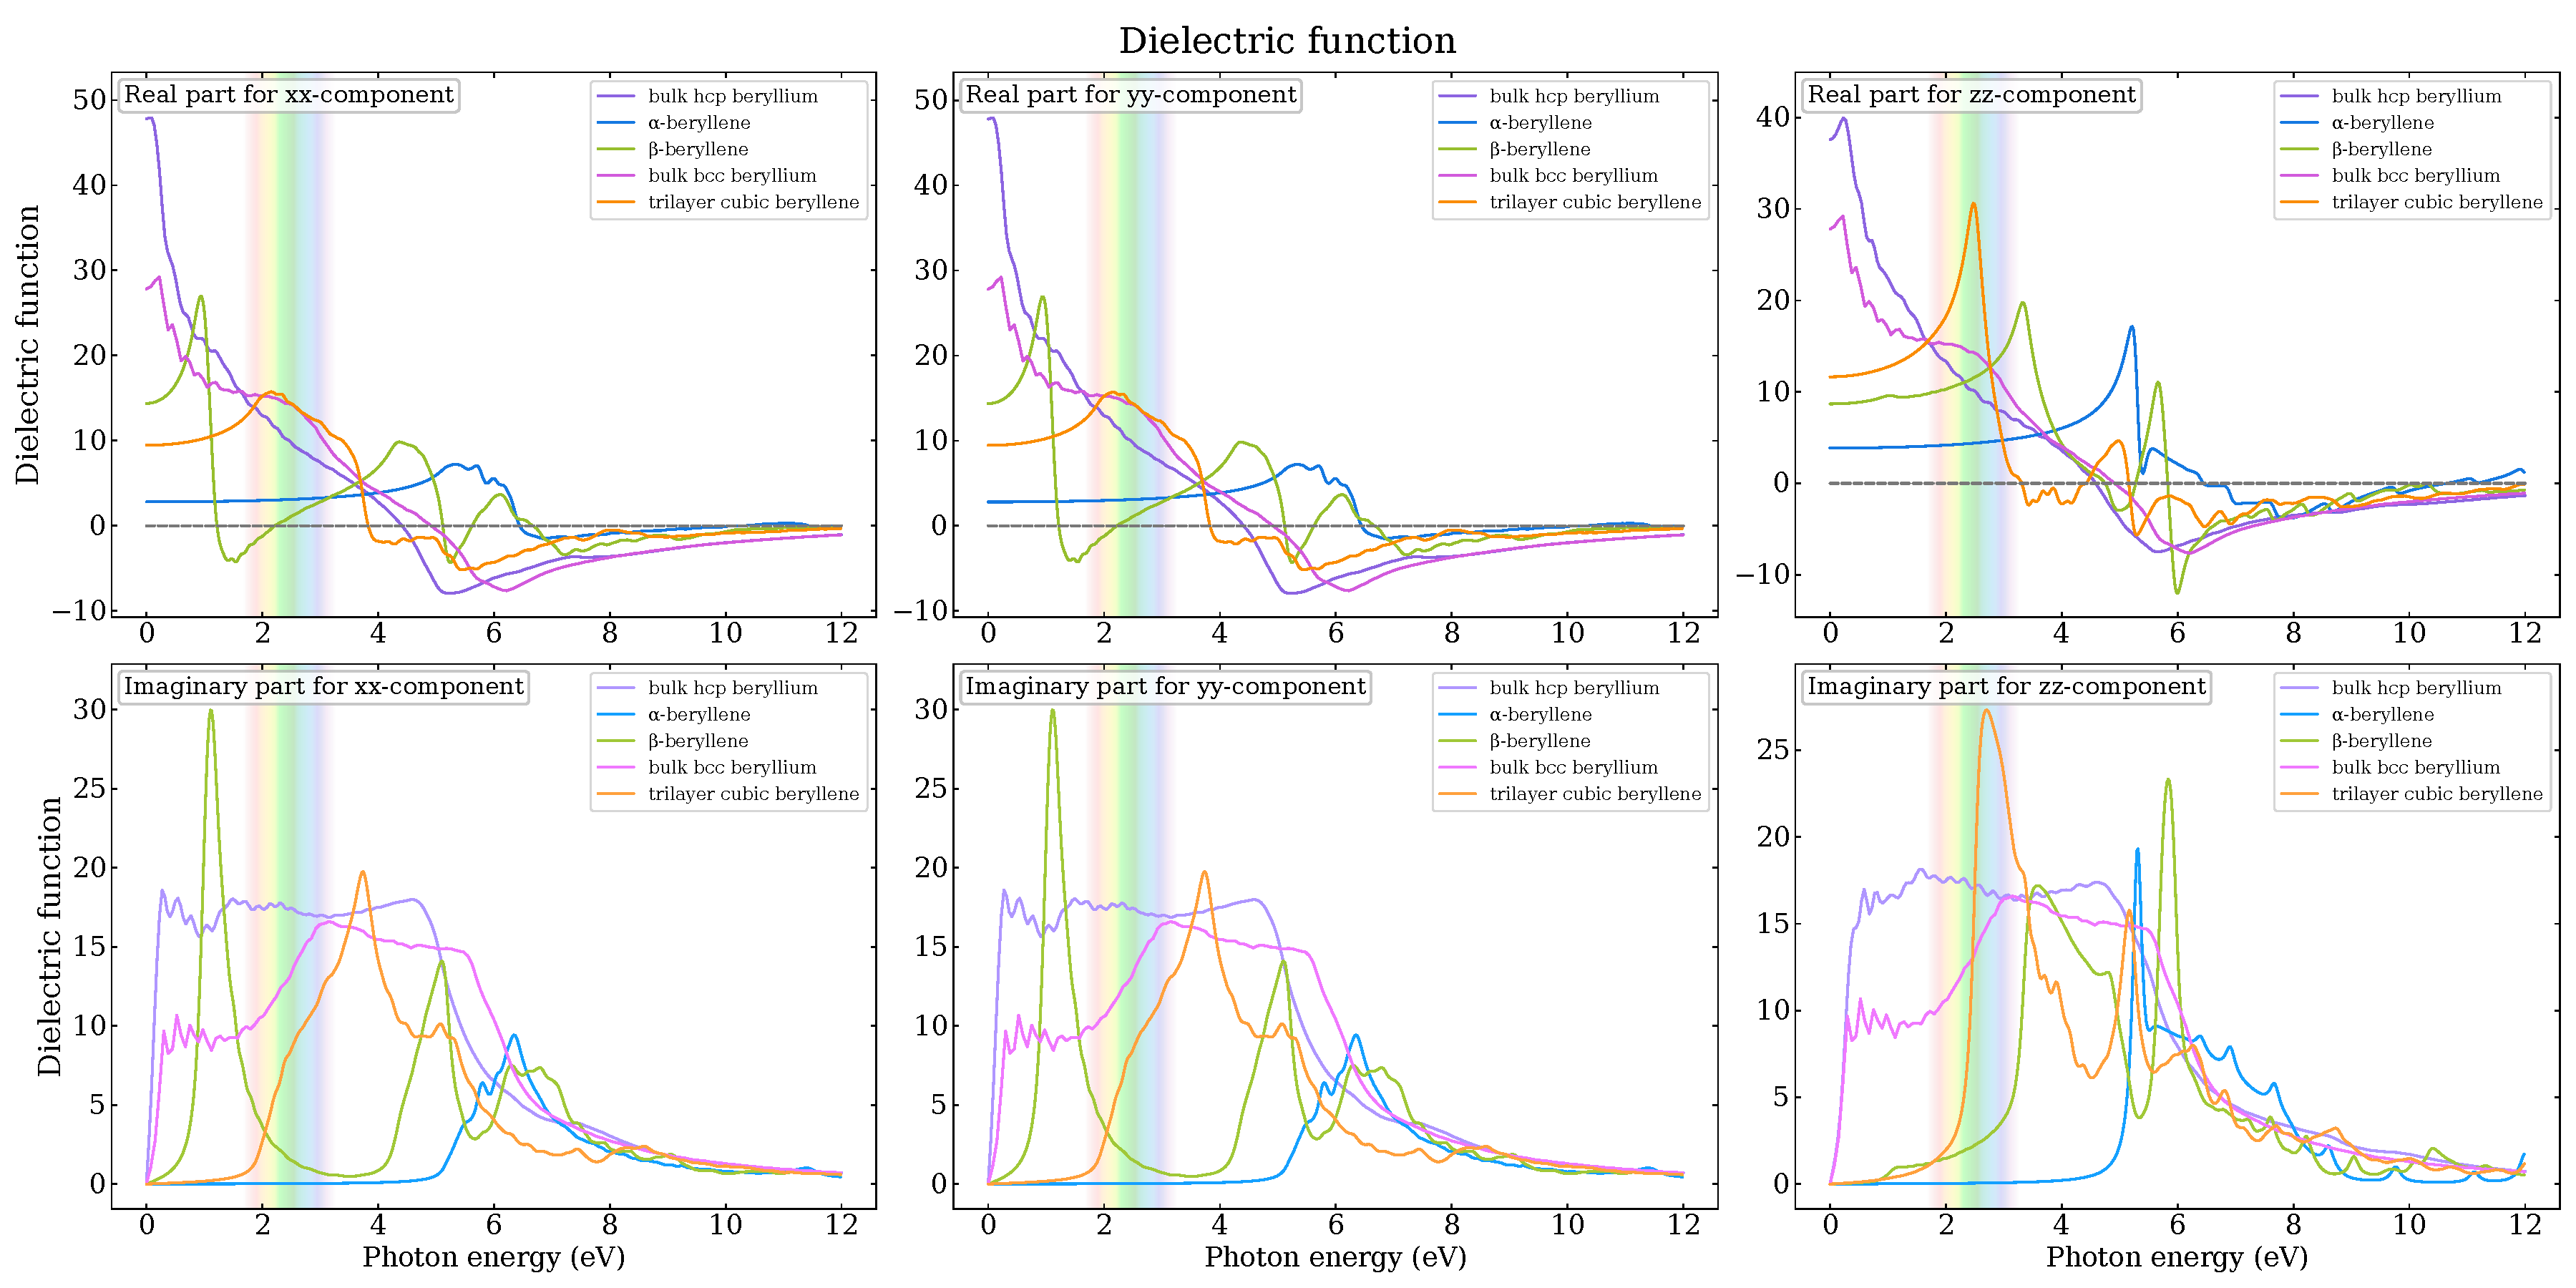
\includegraphics[width=0.95\linewidth]{figures_proj3/dielectric_pristine_thesis.pdf}
\caption{Real and imaginary parts of the dielectric function for bulk hcp beryllium,
bulk bcc beryllium,
$\alpha$-beryllene,
$\beta$-beryllene,
and trilayer cubic beryllene.
The spectra are shown for the $xx$,
$yy$,
and $zz$ components as functions of photon energy.}
\label{fig:proj3_bulk_cubic_dielectric}
\end{figure}

The absorption coefficient and energy-loss spectra are shown in figure~\ref{fig:proj3_bulk_cubic_abs_loss}.
Trilayer cubic beryllene shows an absorption enhancement relative to bulk bcc beryllium only in some directions and energy ranges.
In the visible interval of \qtyrange{1.65}{3.26}{\electronvolt},
the trilayer $xx$ and $yy$ absorption is lower than that of bulk bcc beryllium at every available trilayer sample.
For this comparison,
the bulk spectrum is linearly interpolated to the trilayer energy grid.
The respective visible maxima are approximately \qty{0.0604}{\per\nano\metre} and \qty{0.0746}{\per\nano\metre}.
The trilayer $zz$ response exceeds the bulk value over only part of this interval.
The strongest sampled absorption of trilayer cubic beryllene occurs near \qty{5.40}{\electronvolt} in $xx$ and $yy$,
and near \qty{5.25}{\electronvolt} in $zz$.
The corresponding coefficients are approximately \qty{0.148}{\per\nano\metre} and \qty{0.166}{\per\nano\metre}, respectively.
These results show a redistribution of the effective interband response.

The energy-loss spectra also differ between directions and structures.
The low-energy $\beta$ in-plane feature and the high-energy $\alpha$ out-of-plane maximum are retained in the comparison.
The scalar energy-loss features identify variations in the inverse dielectric response, and propagating plasmon modes require a separate analysis.

\begin{figure}[!htbp]
\centering
    \adjustbox{valign=c}{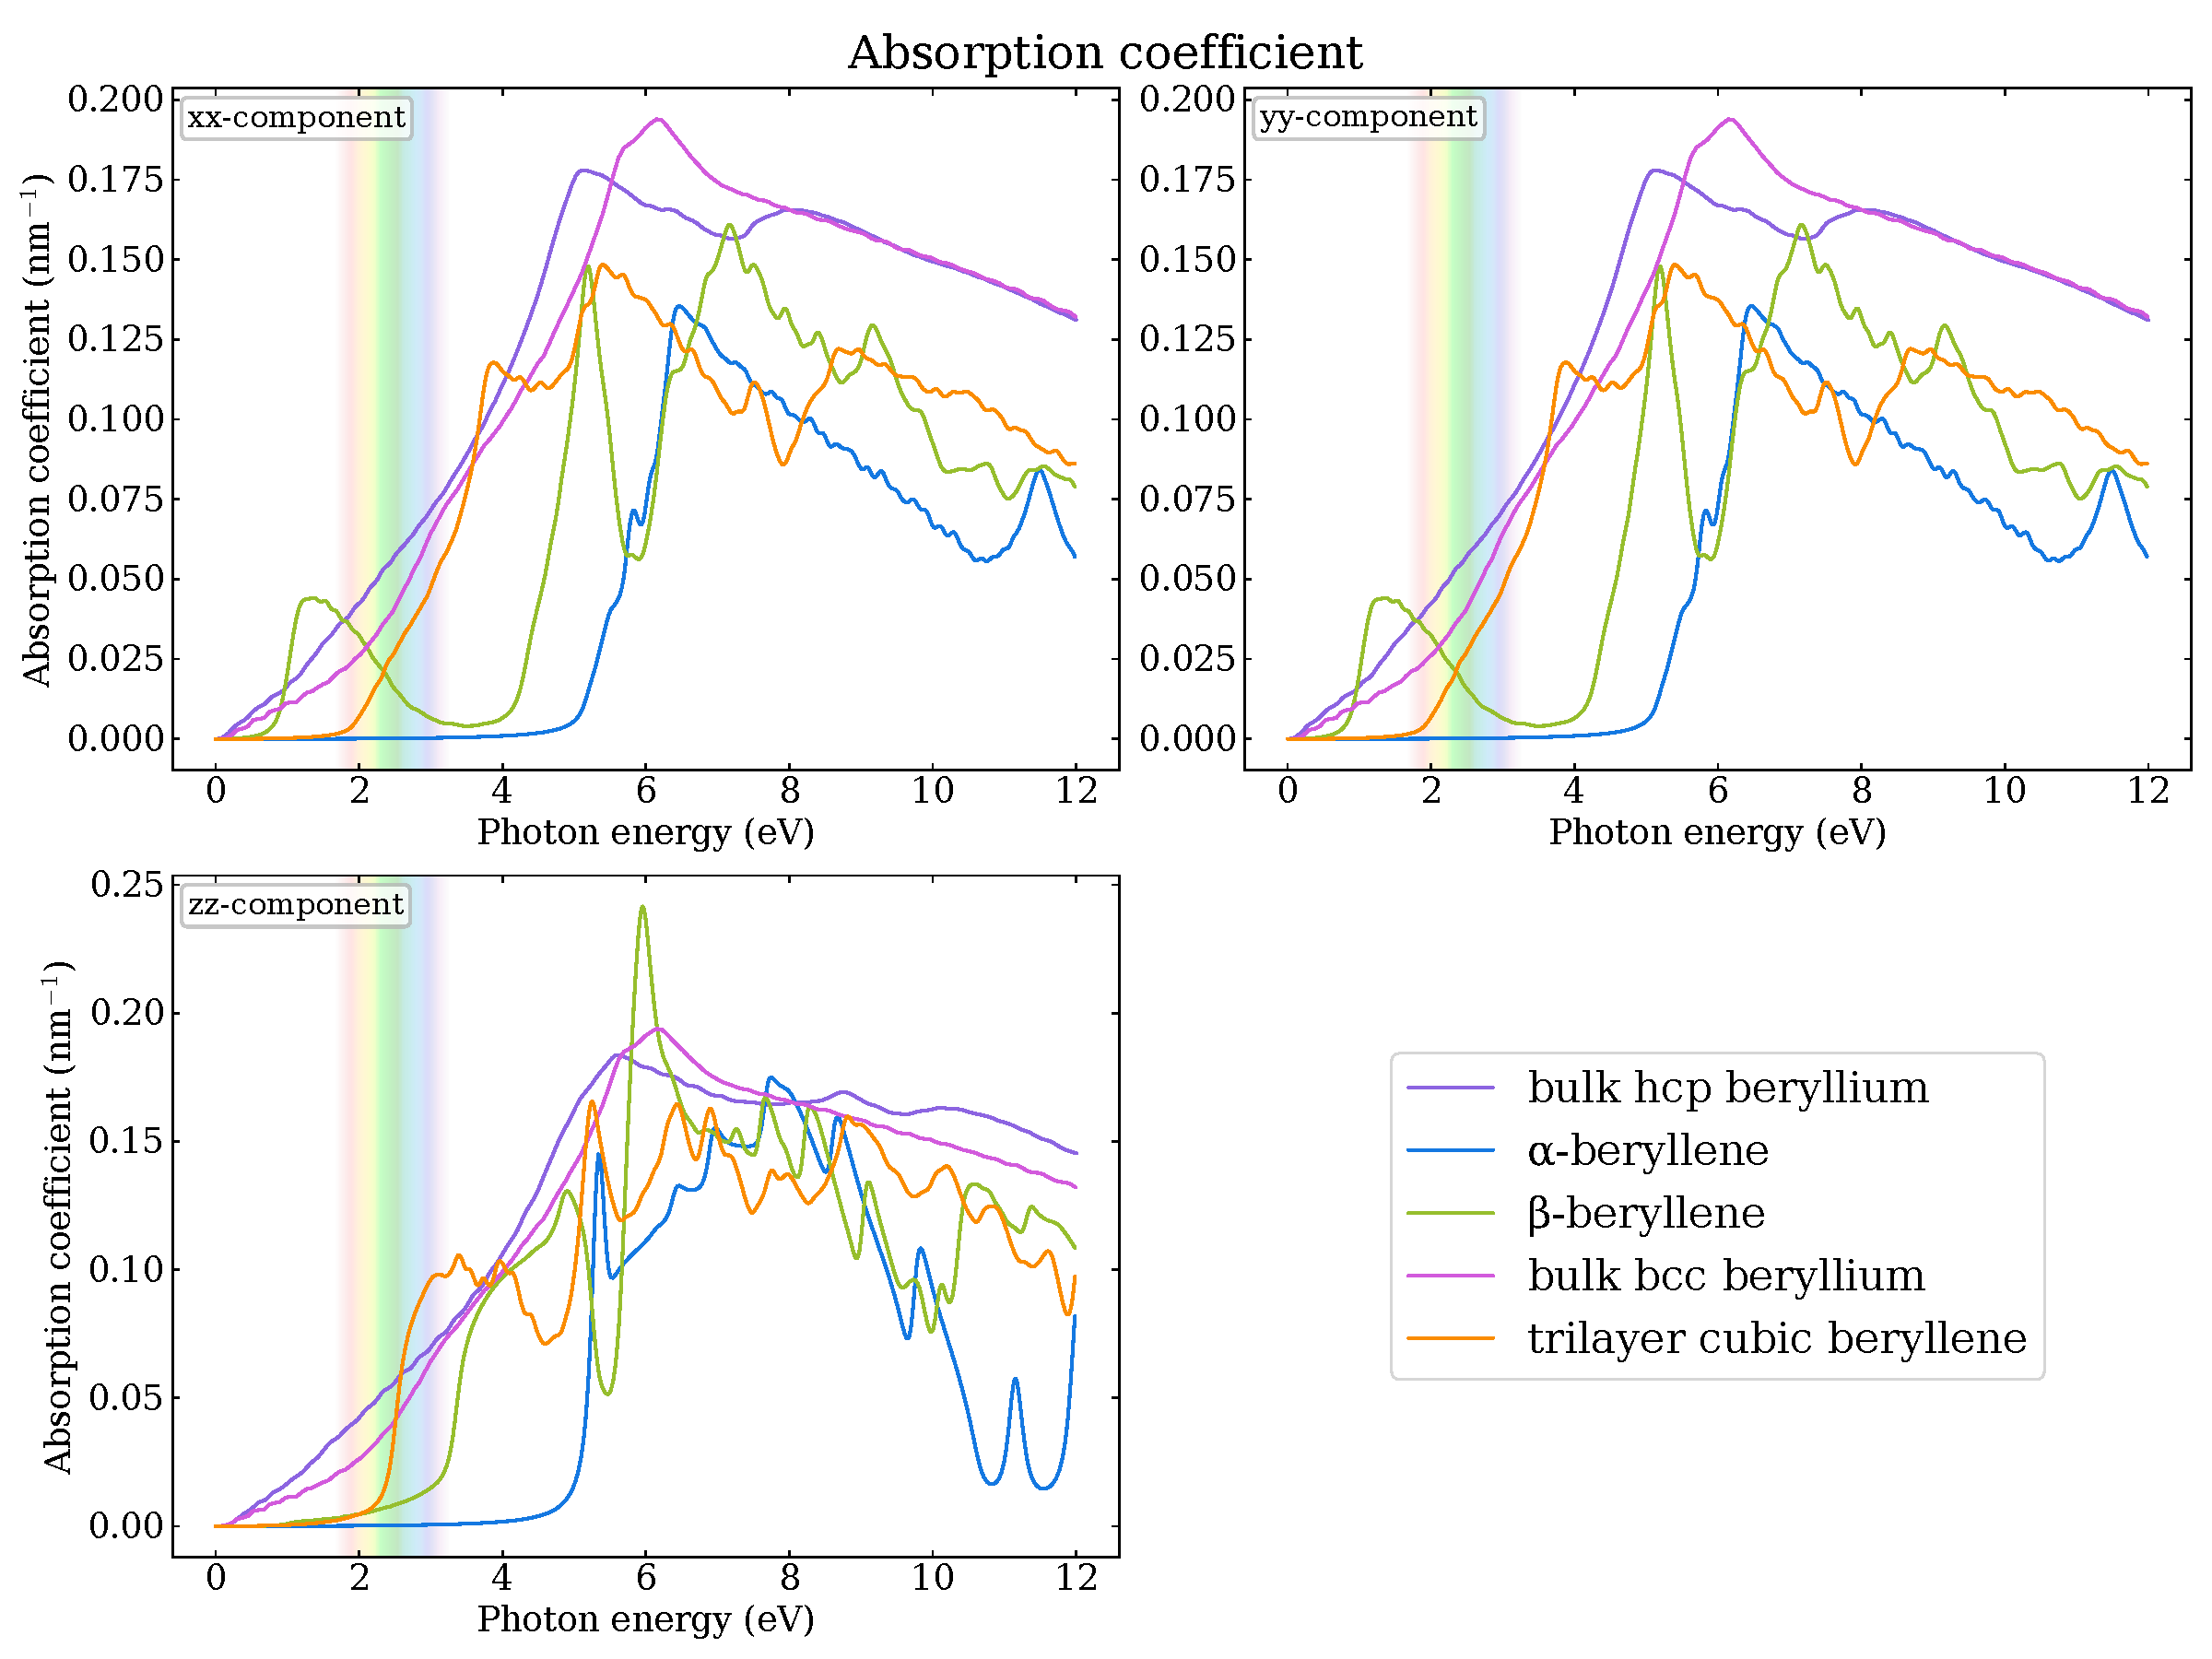
\includegraphics[width=0.80\linewidth]{figures_proj3/optics_pristine_absorption_thesis.pdf}}%
    \par\nointerlineskip
    \adjustbox{valign=c}{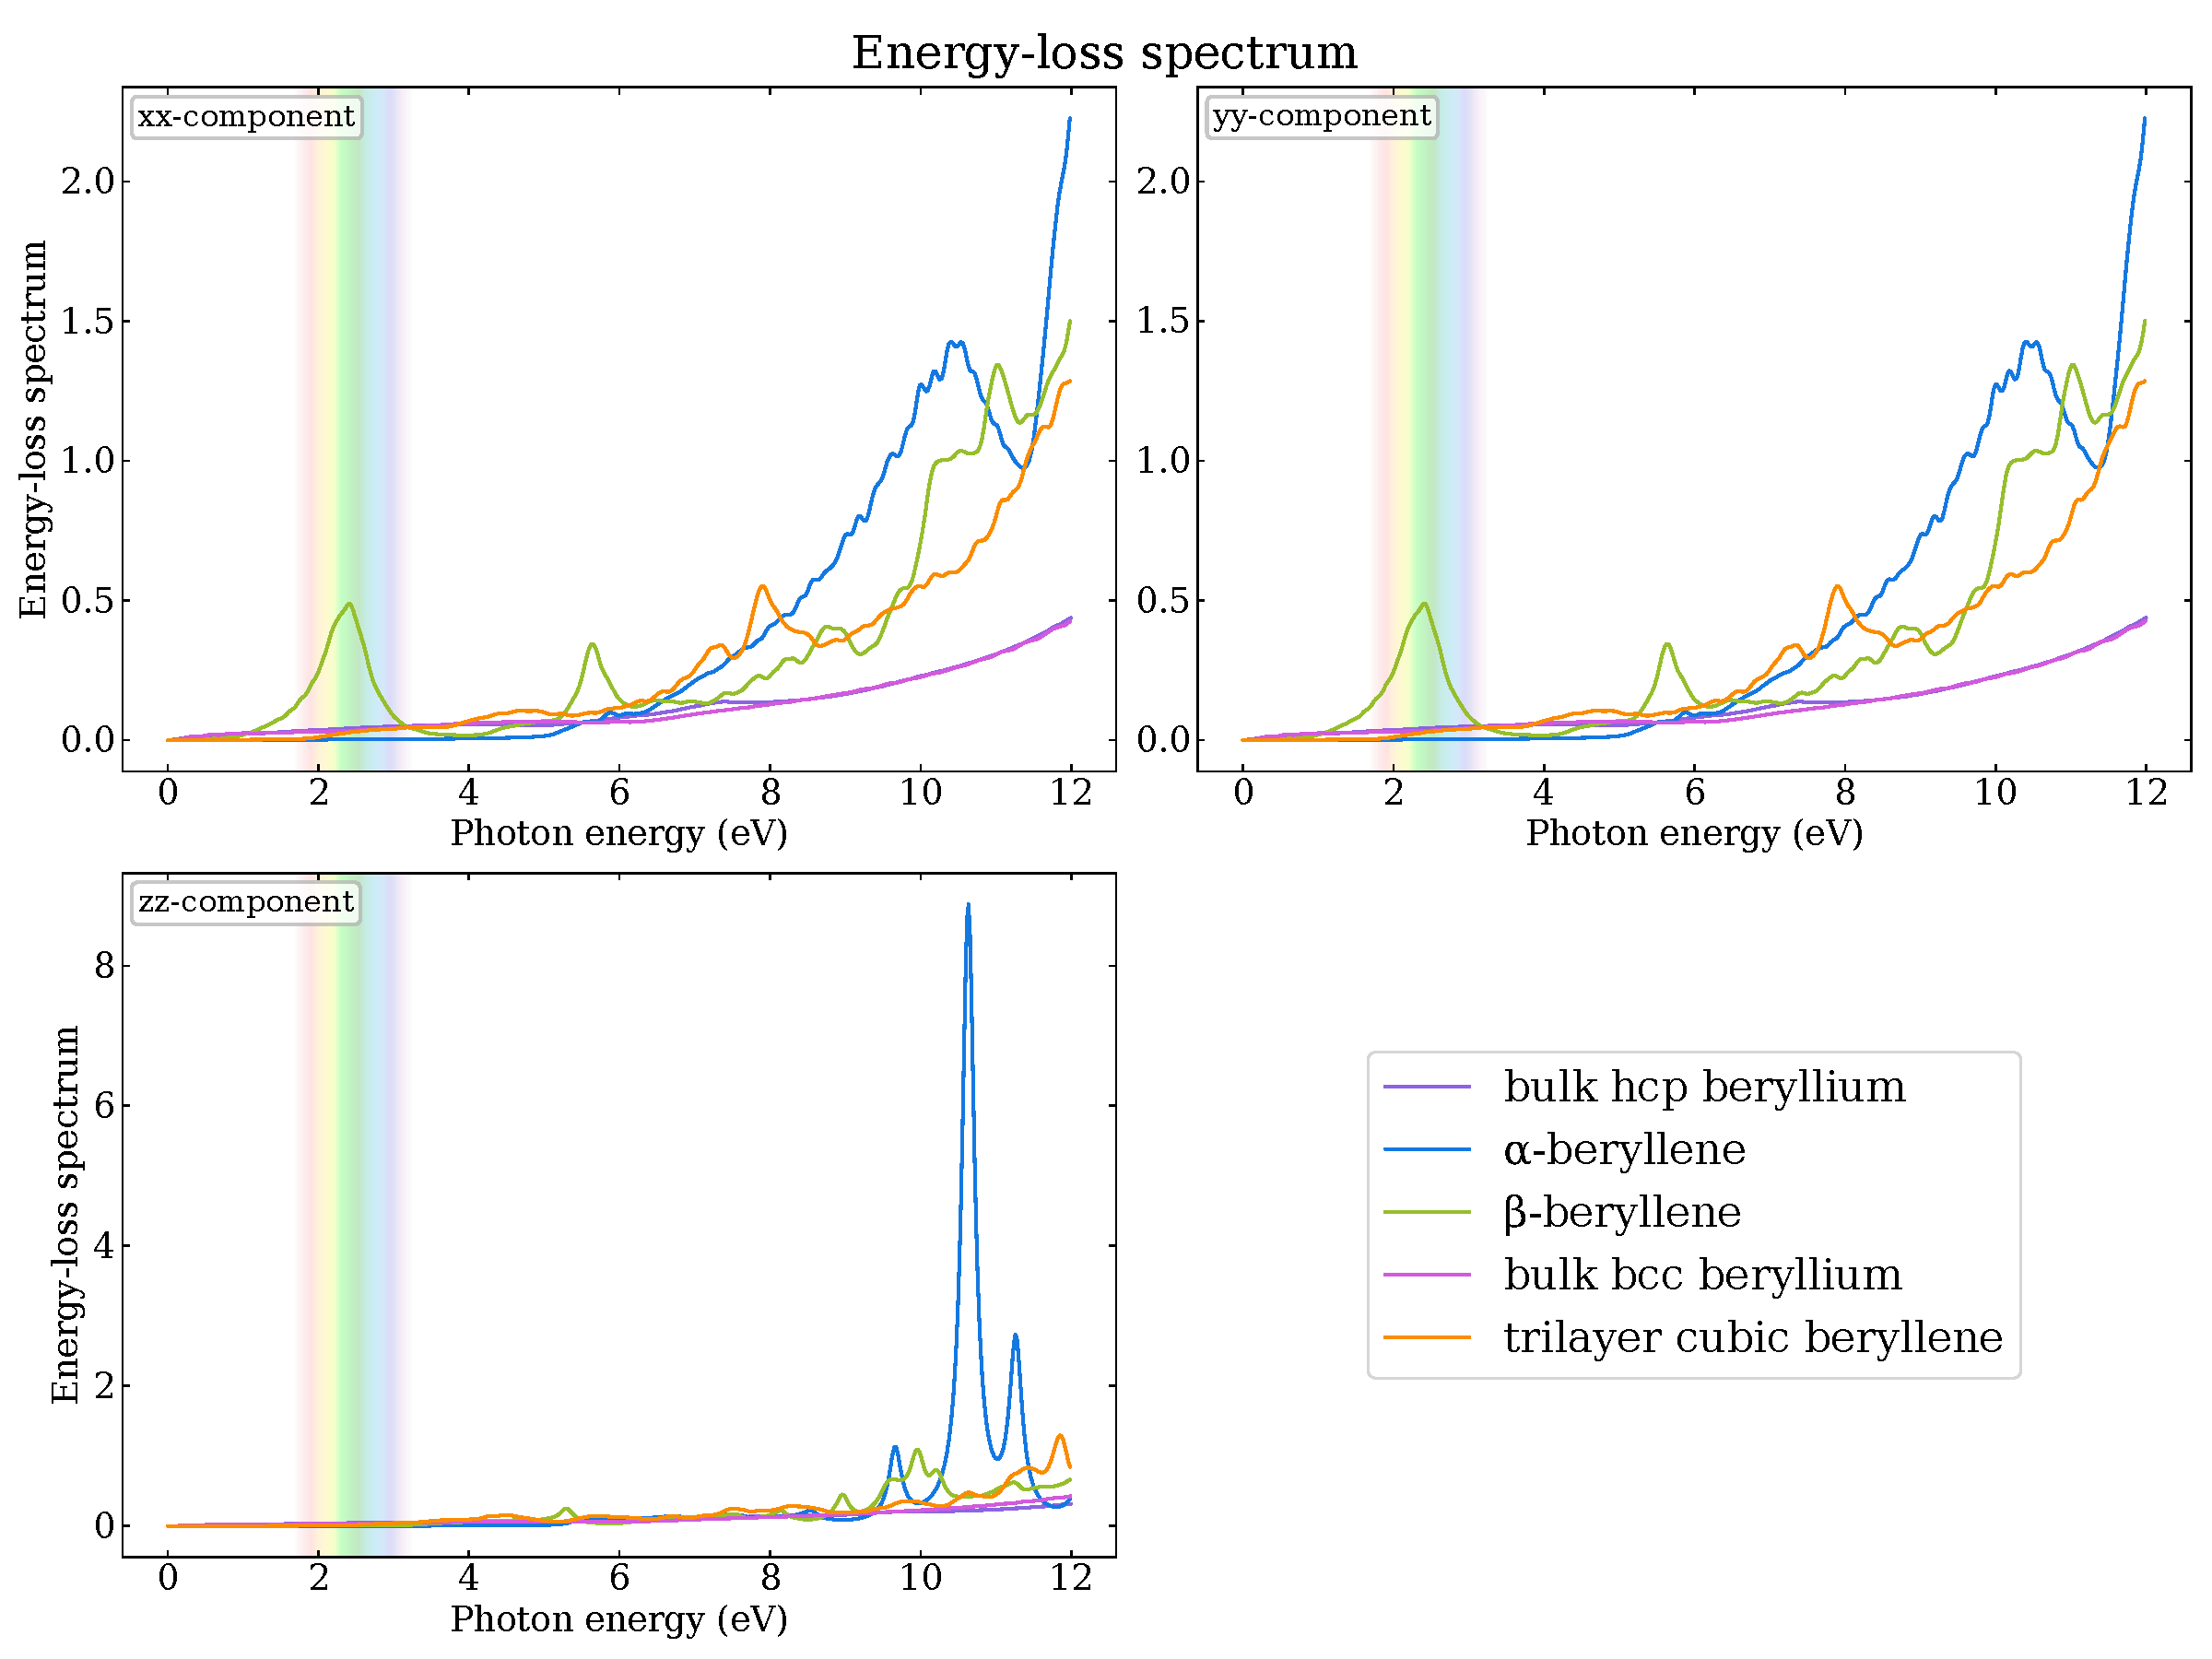
\includegraphics[width=0.80\linewidth]{figures_proj3/optics_pristine_energy-loss_thesis.pdf}}%
\caption{Absorption coefficient and energy-loss spectrum for bulk hcp beryllium,
bulk bcc beryllium,
$\alpha$-beryllene,
$\beta$-beryllene,
and trilayer cubic beryllene.
Upper: absorption coefficient ($\mathrm{nm}^{-1}$). Lower: energy-loss spectrum.
The spectra are shown for the $xx$,
$yy$,
and $zz$ components as functions of photon energy.}
\label{fig:proj3_bulk_cubic_abs_loss}
\end{figure}

\subsubsection{Hydrogen-functionalized beryllene structures}
\label{3_optical_hydrogenated_structures}

We now examine the effect of hydrogen adsorption on the optical properties of $\alpha$-beryllene and $\beta$-beryllene.
The real and imaginary parts of the dielectric function for the pristine and hydrogen-functionalized structures are shown in figure~\ref{fig:proj3_hydrogenated_dielectric}.

For $\alpha$-beryllene,
hydrogen adsorption changes the magnitude and spectral distribution of the effective dielectric response.
In $xx$ and $yy$, 2H-$\alpha$-beryllene has a real dielectric maximum of approximately 31.2 near \qty{4.91}{\electronvolt},
and its strongest imaginary dielectric feature is approximately 31.2 near \qty{5.59}{\electronvolt}.
In $zz$, the largest imaginary dielectric feature instead occurs near \qty{9.77}{\electronvolt}.
These comparisons retain the specified H/H surface-radius convention for the hydrogen-functionalized layer.
Changes in peak height therefore describe an effective response under that convention.

For $\beta$-beryllene,
single- and double-sided hydrogen adsorption redistribute the dielectric response and change its directional dependence.
Double-sided adsorption produces distinct spectra in all three Cartesian components.
The strongest imaginary dielectric features occur near \qty{6.59}{\electronvolt} in $xx$,
\qty{9.26}{\electronvolt} in $yy$, and \qty{8.24}{\electronvolt} in $zz$,
with values of approximately 14.96, 7.68, and 14.97, respectively.
The first real-part sign changes occur near \qty{6.64}{\electronvolt}, \qty{9.32}{\electronvolt}, and \qty{8.10}{\electronvolt}, respectively.
Thus, increasing hydrogen coverage changes the spectral distribution and in-plane anisotropy,
and the peak energies, zero crossings, and enhancements differ between components.
The imaginary dielectric peaks also differ from the maxima of the derived absorption coefficient.

\begin{figure}[!htbp]
\centering
    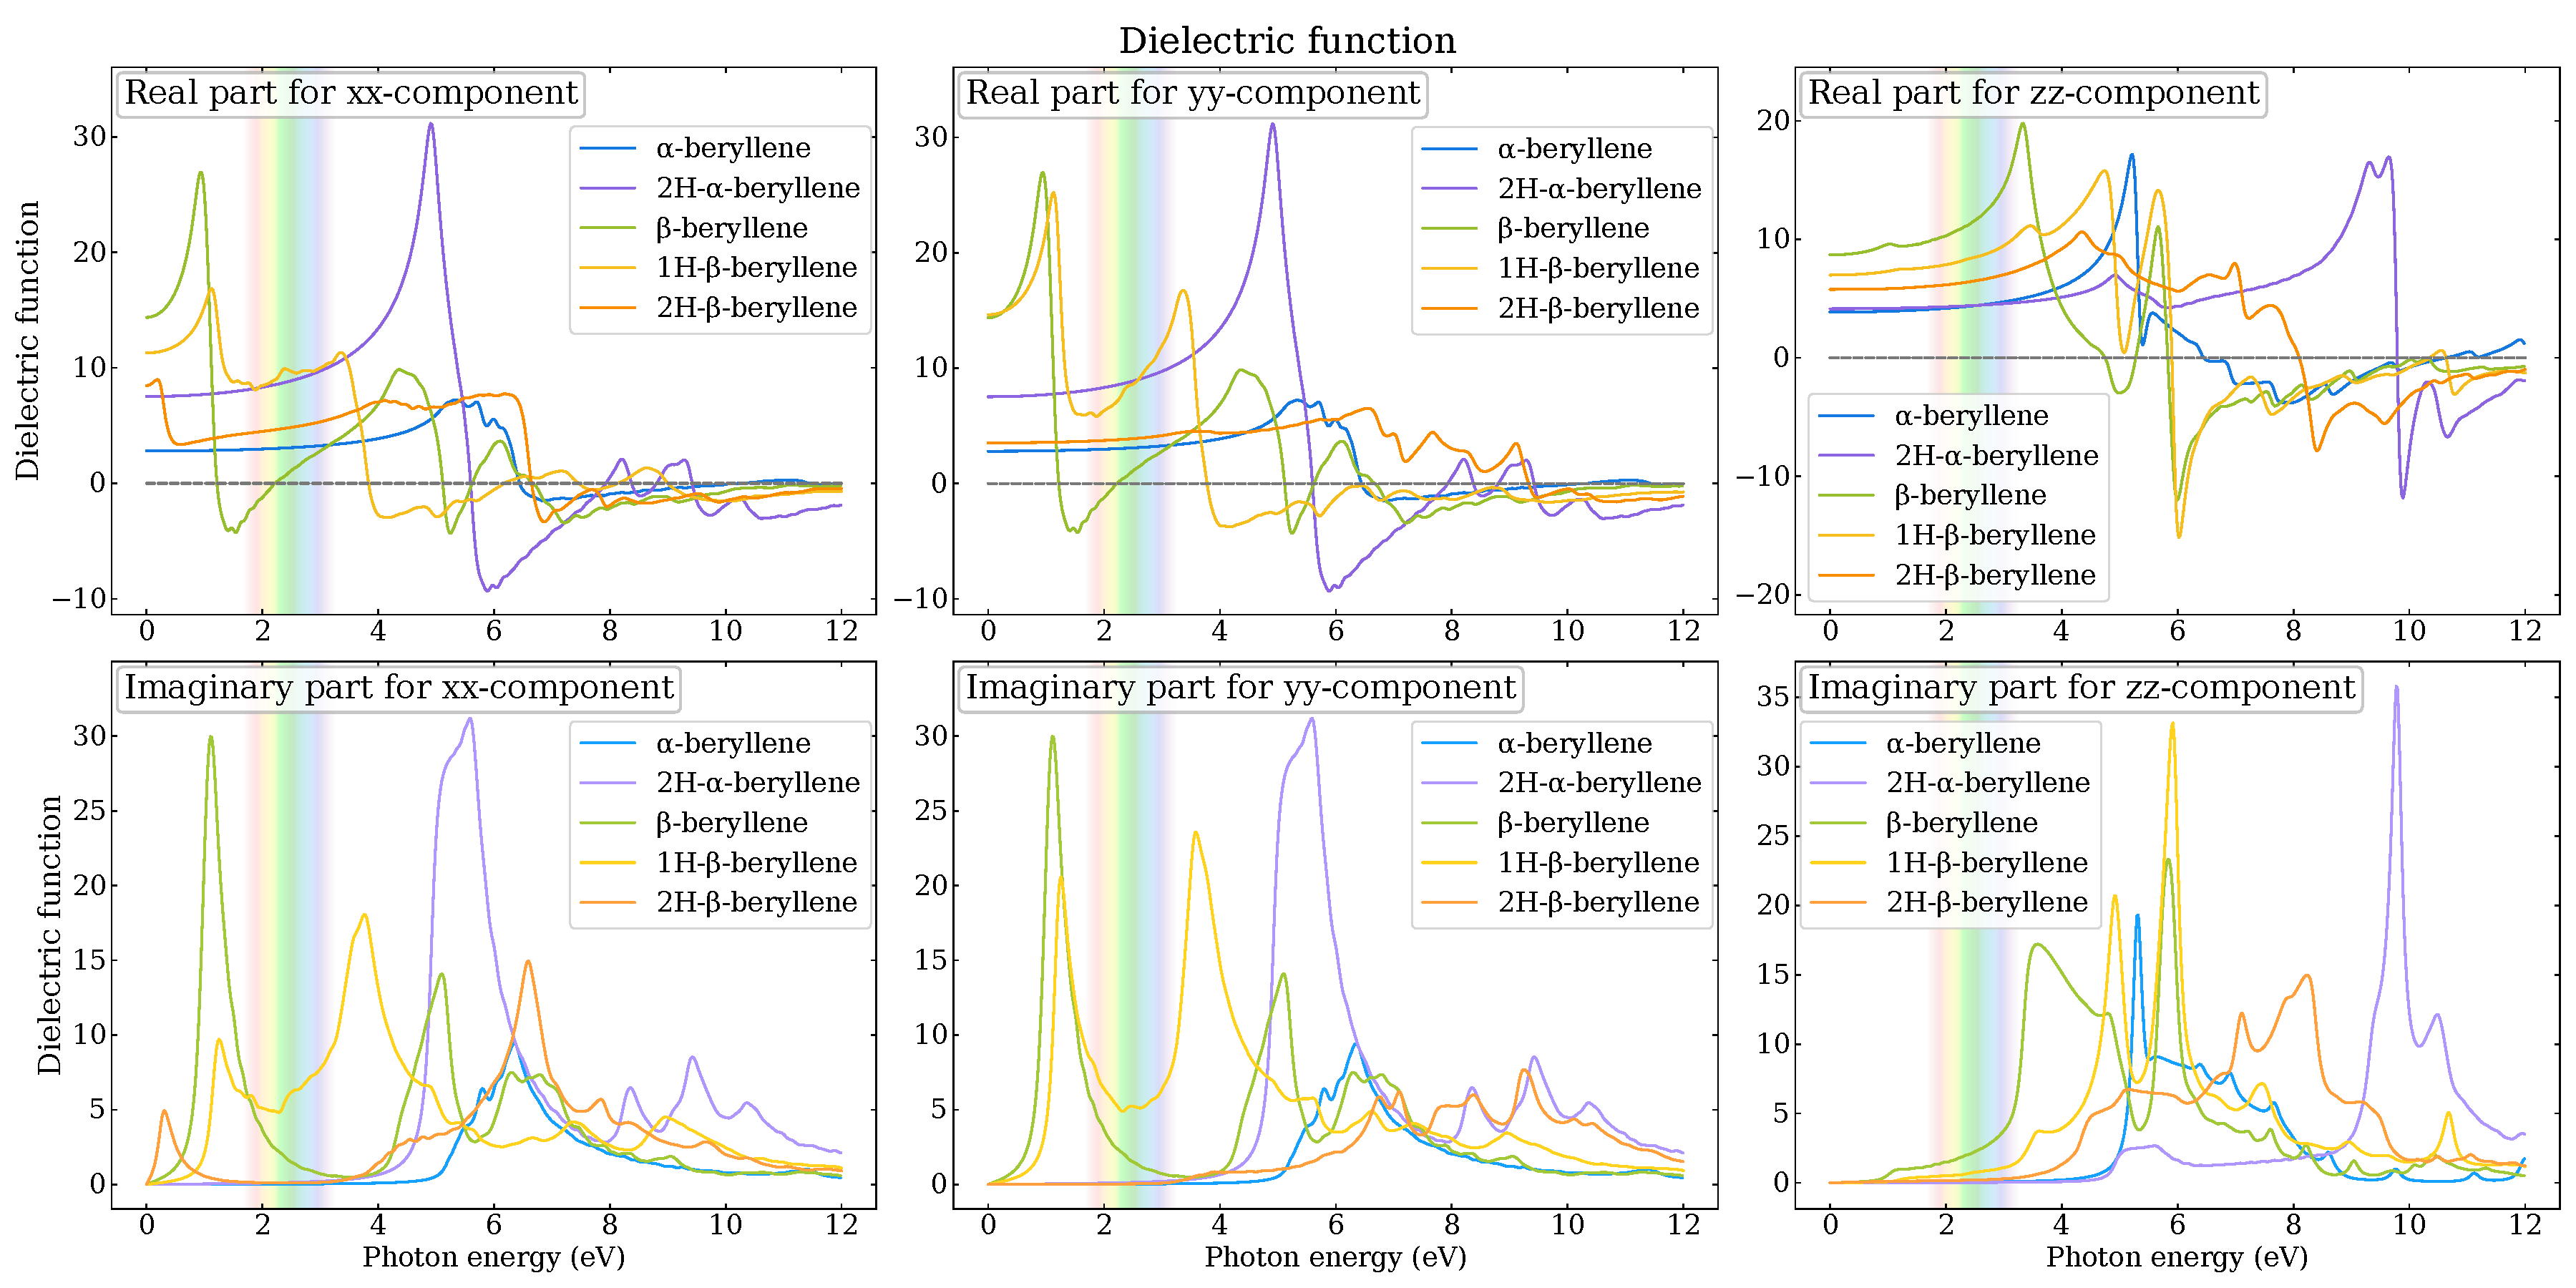
\includegraphics[width=1\linewidth]{figures_proj3/dielectric_hydrogenated_thesis.pdf}
\caption{Real and imaginary parts of the dielectric function for pristine and hydrogen-functionalized $\alpha$- and $\beta$-beryllene structures.
The spectra are shown for the $xx$,
$yy$,
and $zz$ components as functions of photon energy.}
\label{fig:proj3_hydrogenated_dielectric}
\end{figure}

The corresponding absorption coefficient and energy-loss spectra are shown in figure~\ref{fig:proj3_hydrogenated_abs_loss}.
For $\alpha$-beryllene, hydrogen adsorption produces a strongly direction-dependent redistribution of absorption.
Relative to pristine $\alpha$-beryllene,
the $xx$ and $yy$ coefficients increase over the sampled visible interval,
but the visible maximum of 2H-$\alpha$-beryllene is only approximately \qty{0.00137}{\per\nano\metre},
much smaller than its ultraviolet maximum near \qty{5.71}{\electronvolt}.
The $zz$ coefficient instead decreases throughout the sampled \qtyrange{1.65}{4.13}{\electronvolt} interval,
and its strongest peak occurs near \qty{9.83}{\electronvolt}.
For 2H-$\beta$-beryllene,
the strongest sampled absorption peaks occur near \qty{6.75}{\electronvolt} in $xx$,
\qty{9.39}{\electronvolt} in $yy$,
and \qty{8.36}{\electronvolt} in $zz$.
The energy-loss spectra likewise change with hydrogen coverage and direction.
These results establish changes in the calculated interband and inverse dielectric response.
The weak low-energy tails arise from the finite numerical broadening.

\begin{figure}[!htbp]
\centering
    \adjustbox{valign=c}{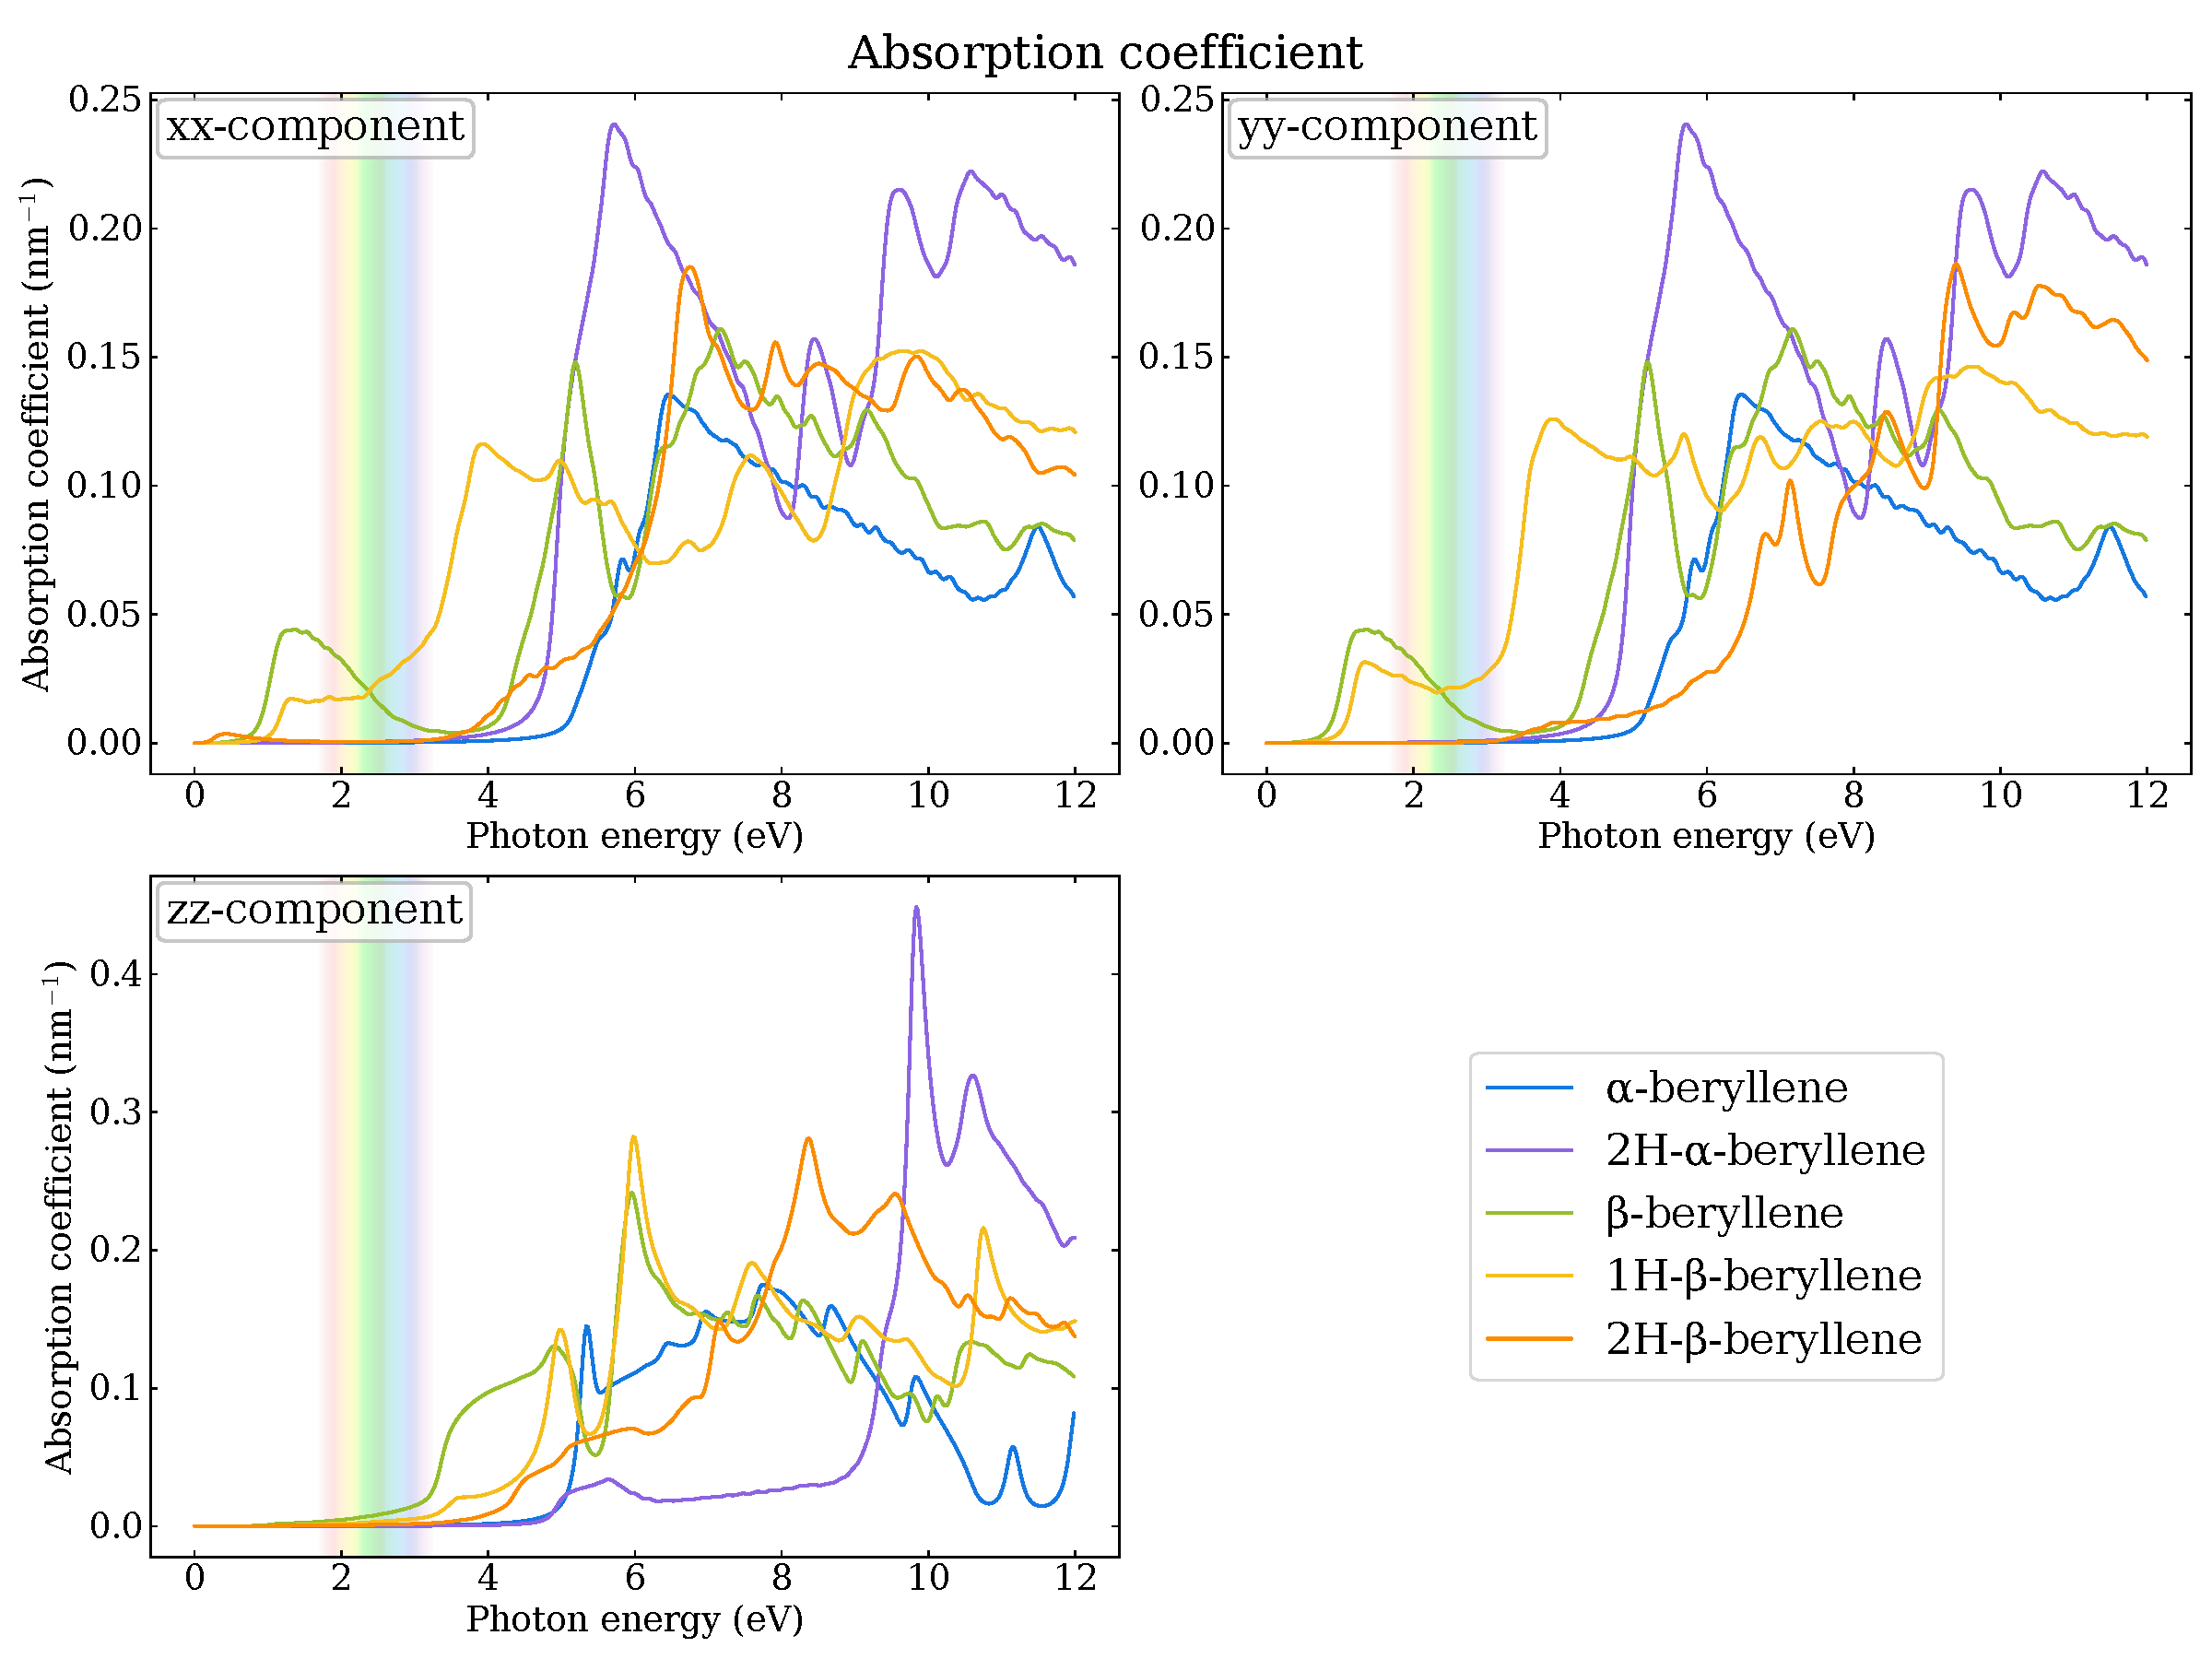
\includegraphics[width=0.80\linewidth]{figures_proj3/optics_hydrogenated_absorption_thesis.pdf}}%
    \par\nointerlineskip
    \adjustbox{valign=c}{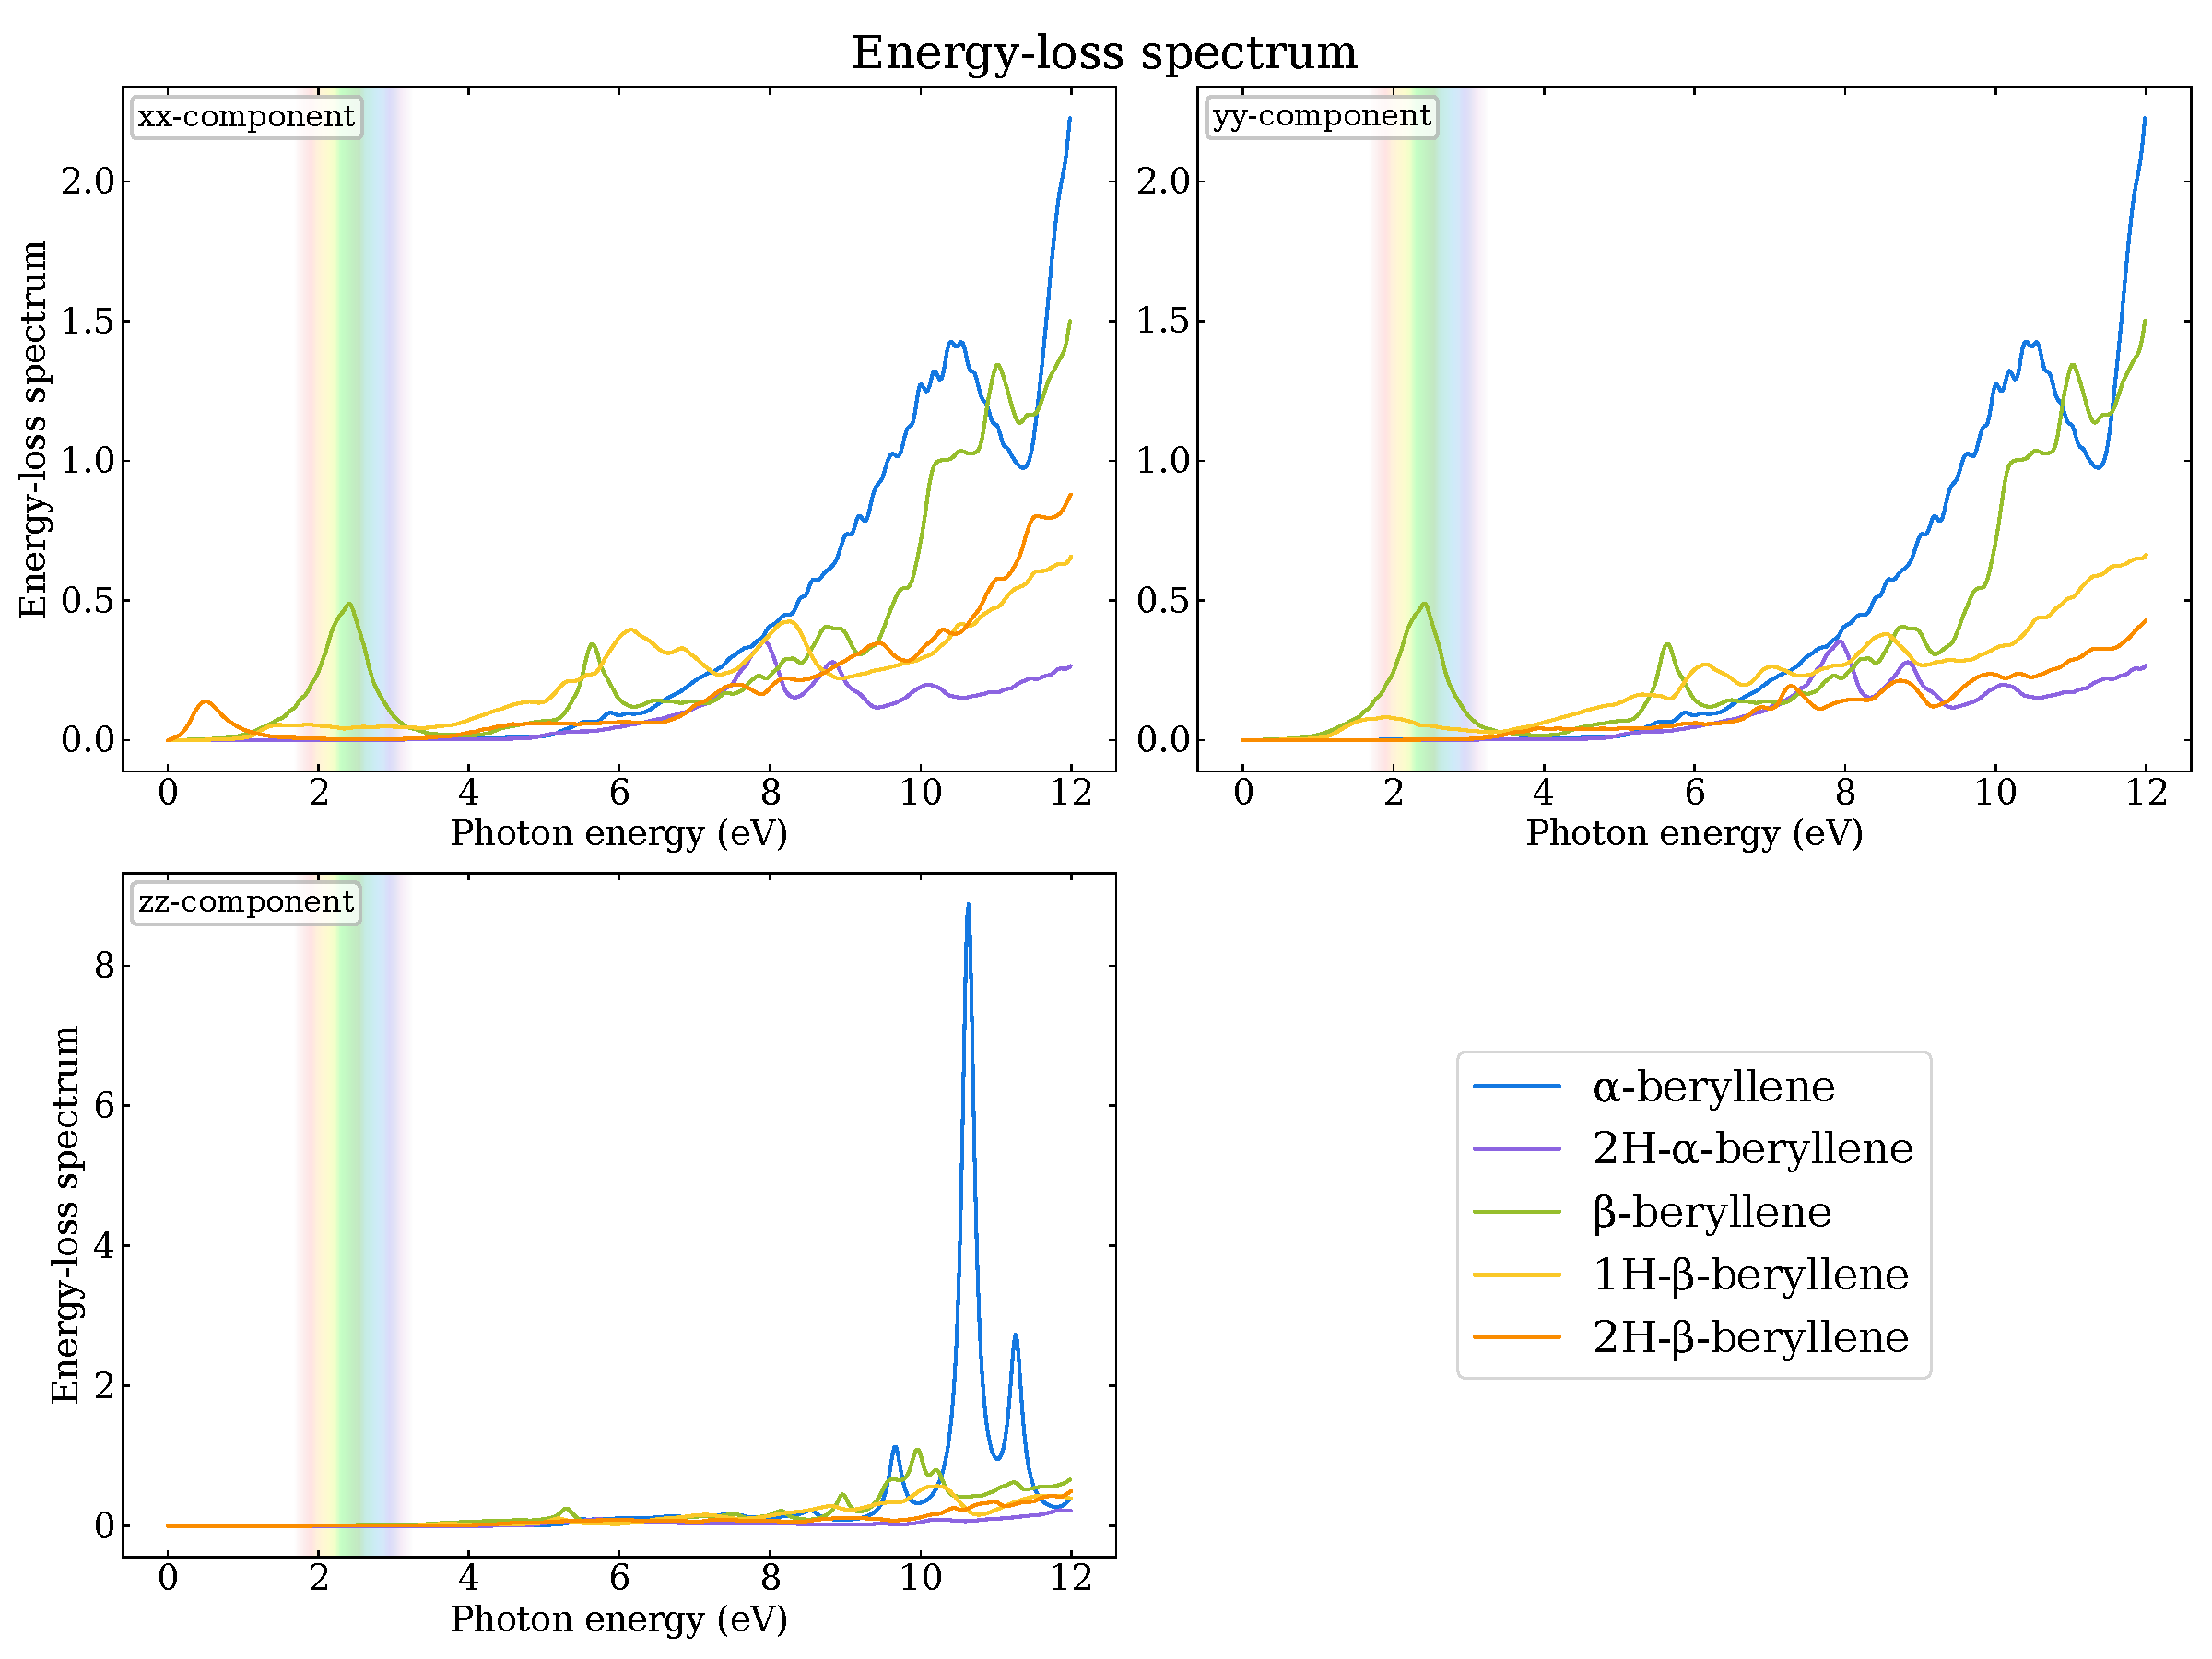
\includegraphics[width=0.80\linewidth]{figures_proj3/optics_hydrogenated_energy-loss_thesis.pdf}}%
\caption{Absorption coefficient and energy-loss spectrum for pristine and hydrogen-functionalized $\alpha$- and $\beta$-beryllene structures.
Upper: absorption coefficient ($\mathrm{nm}^{-1}$). Lower: energy-loss spectrum.
The spectra are shown for the $xx$,
$yy$,
and $zz$ components as functions of photon energy,
using the scalar definitions described in section~\ref{3_methods}.}
\label{fig:proj3_hydrogenated_abs_loss}
\end{figure}

These results show that both dimensionality and hydrogen functionalization redistribute the effective interband optical response of beryllene.
Pristine $\alpha$- and $\beta$-beryllene exhibit pronounced anisotropy,
while trilayer cubic beryllene and the hydrogen-functionalized structures enhance some components and reduce others.

\section{Conclusions}
\label{3_conclusions}

In this chapter,
we investigated the structural stability,
electronic structure,
optical response,
topological properties,
and superconductivity of pristine and hydrogen-functionalized two-dimensional beryllium phases using first-principles density functional theory calculations.
Alongside the previously reported $\alpha$- and $\beta$-beryllene structures,
we identified a dynamically stable trilayer cubic beryllene phase.
The phonon-dispersion calculations also confirm the dynamical stability of 2H-$\alpha$-beryllene,
whereas the interpolated imaginary frequencies near $\Gamma$ leave the long-wavelength stability of 1H-$\beta$-beryllene unresolved.
2H-$\beta$-beryllene has a harmonic soft mode,
and a one-mode anharmonic treatment supports suppression of a static distortion along this mode by quantum fluctuations.
The full anharmonic stability depends on the coupling between modes.
The molecular dynamics simulations show that all three hydrogen-functionalized structures persist at \qty{300}{\kelvin} over \qty{5.5}{\pico\second}.

Hydrogen functionalization substantially modifies the structural and electronic properties of beryllene.
In particular,
it transforms metallic $\alpha$-beryllene into 2H-$\alpha$-beryllene,
a wide-gap semiconductor with an HSE06 band gap of \qty{6.00}{\electronvolt},
whereas the hydrogen-functionalized $\beta$-beryllene structures retain metallic behaviour.
The calculated adsorption energies show that hydrogen adsorption is exothermic with respect to molecular hydrogen.
Including zero-point and thermal contributions,
only 2H-$\alpha$-beryllene is thermodynamically stable against \ce{H2} release under ambient conditions.
2H-$\beta$-beryllene requires an elevated \ce{H2} pressure,
whereas persistence of 1H-$\beta$-beryllene under ambient conditions would require kinetic trapping.

The calculated optical properties show a direction-dependent redistribution of the effective interband response after dimensional reduction and hydrogen functionalization.
Pristine $\alpha$- and $\beta$-beryllene exhibit pronounced anisotropy and distinct energy-loss features.
Trilayer cubic beryllene absorbs more strongly than bulk bcc beryllium only in some directions and energy ranges,
and hydrogen adsorption enhances some components while reducing others.
These comparisons use the Cartesian diagonal dielectric components and exclude a Drude intraband contribution.

Parity analysis of the spin-orbit-coupled electronic states confirms the previously reported non-trivial topology of $\alpha$-beryllene and the trivial topology of $\beta$-beryllene.
Trilayer cubic beryllene also has a non-trivial $\mathbb{Z}_2$ index,
whereas all hydrogen-functionalized structures are trivial.
As the non-trivial subspaces of these metallic phases are isolated only by spin-orbit gaps of approximately \qty{1}{\milli\electronvolt} above the Fermi level,
these indices are conditional screening results for band inversions.

In addition to the earlier predictions for $\alpha$- and $\beta$-beryllene~\cite{li2023coexistence},
electron-phonon calculations predict phonon-mediated superconductivity in trilayer cubic beryllene, 1H-$\beta$-beryllene, and 2H-$\beta$-beryllene.
Trilayer cubic beryllene is a weak-coupling superconductor with $T_\mathrm{c}^{\mathrm{iso}}=\qty{3.7}{\kelvin}$.
2H-$\beta$-beryllene has the strongest coupling, $\lambda=1.40$,
and the highest transition temperatures, \qty{28.3}{\kelvin} from the isotropic and approximately \qty{31.7}{\kelvin} from the anisotropic Migdal--Eliashberg equations.
For 1H-$\beta$-beryllene, the gap anisotropy raises $T_\mathrm{c}$ from \qty{11.6}{\kelvin} to approximately \qty{14.2}{\kelvin}.
The electron-phonon calculations of 2H-$\beta$-beryllene use a structure relaxed with the D3 dispersion correction,
in which the soft mode is absent.
For trilayer cubic beryllene and 2H-$\beta$-beryllene,
the coupling strengths exclude the phonon modes below \qty{40}{\per\centi\metre}.

Together,
these results identify two-dimensional beryllium as an elemental platform,
where structural design and hydrogen functionalization tune the electronic structure,
the optical response,
the band inversions of selected subspaces,
and the superconducting transition temperature.

\clearpage
\section{Data availability statement}

The original data presented in this chapter are openly available from the \texttt{GitHub} repository:
\href{https://github.com/Photonico/H-Beryllene_20250718}{\texttt{Photonico/H-Beryllene\_20250718}}.

\section{Supplementary information}
\label{3_supplementary}

Convergence tests for the cohesive energy and total energy are shown in figures~\ref{fig:proj3_cohesive_energy_convergence}
and~\ref{fig:proj3_total_energy_convergence},
respectively,
as functions of the k-point mesh for the beryllium structures.
Convergence tests for the calculation of the dielectric function are shown in figures~\ref{fig:proj3_hcp_dielectric_nbands_convergence}--\ref{fig:proj3_cubic_dielectric_kpoint_convergence},
including tests for both the k-point mesh and the total number of bands included through the parameter \texttt{NBANDS}.

We also test the sensitivity of the cohesive energies to dispersion by adding the D3 energy with Becke--Johnson damping at the PBE geometries.
The cohesive energies of $\alpha$-beryllene, $\beta$-beryllene, and trilayer cubic beryllene then lie \qty{1.04}{\electronvolt}, \qty{0.60}{\electronvolt}, and \qty{0.56}{\electronvolt} per atom above that of bulk hcp beryllium.
Without the correction, these differences are \qty{0.79}{\electronvolt}, \qty{0.44}{\electronvolt}, and \qty{0.43}{\electronvolt} per atom.
The correction therefore favours the bulk phase and preserves the energy ordering.

\begin{figure}[!htbp]
\centering
\begin{tabular}{@{}cc@{}}
    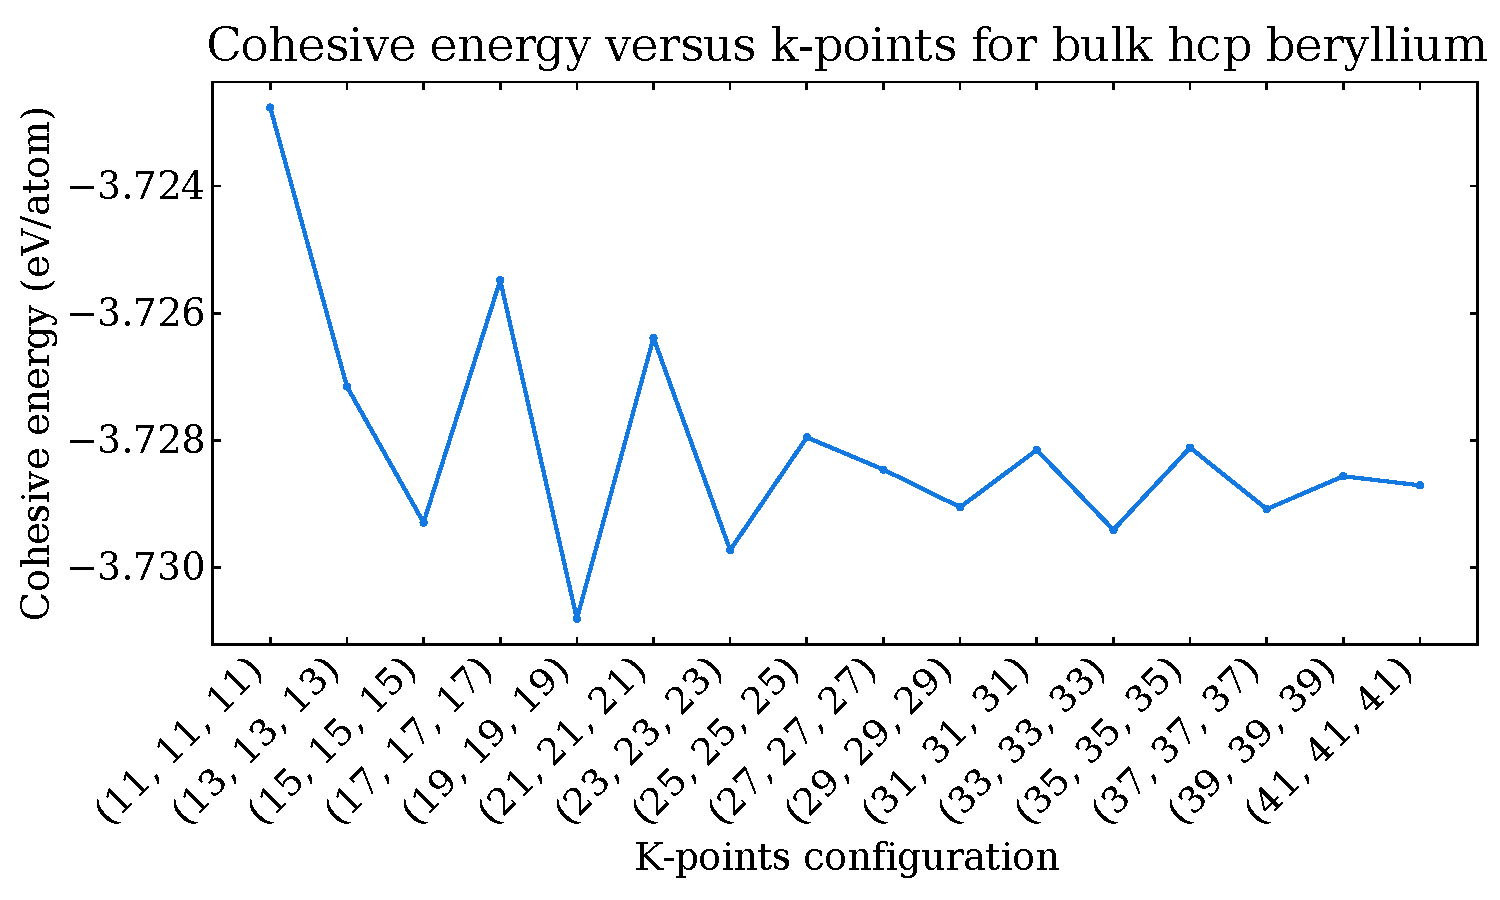
\includegraphics[width=0.40\linewidth]{figures_proj3/convergence_cohesive_kpoints_hcp-beryllium_thesis.pdf}&
    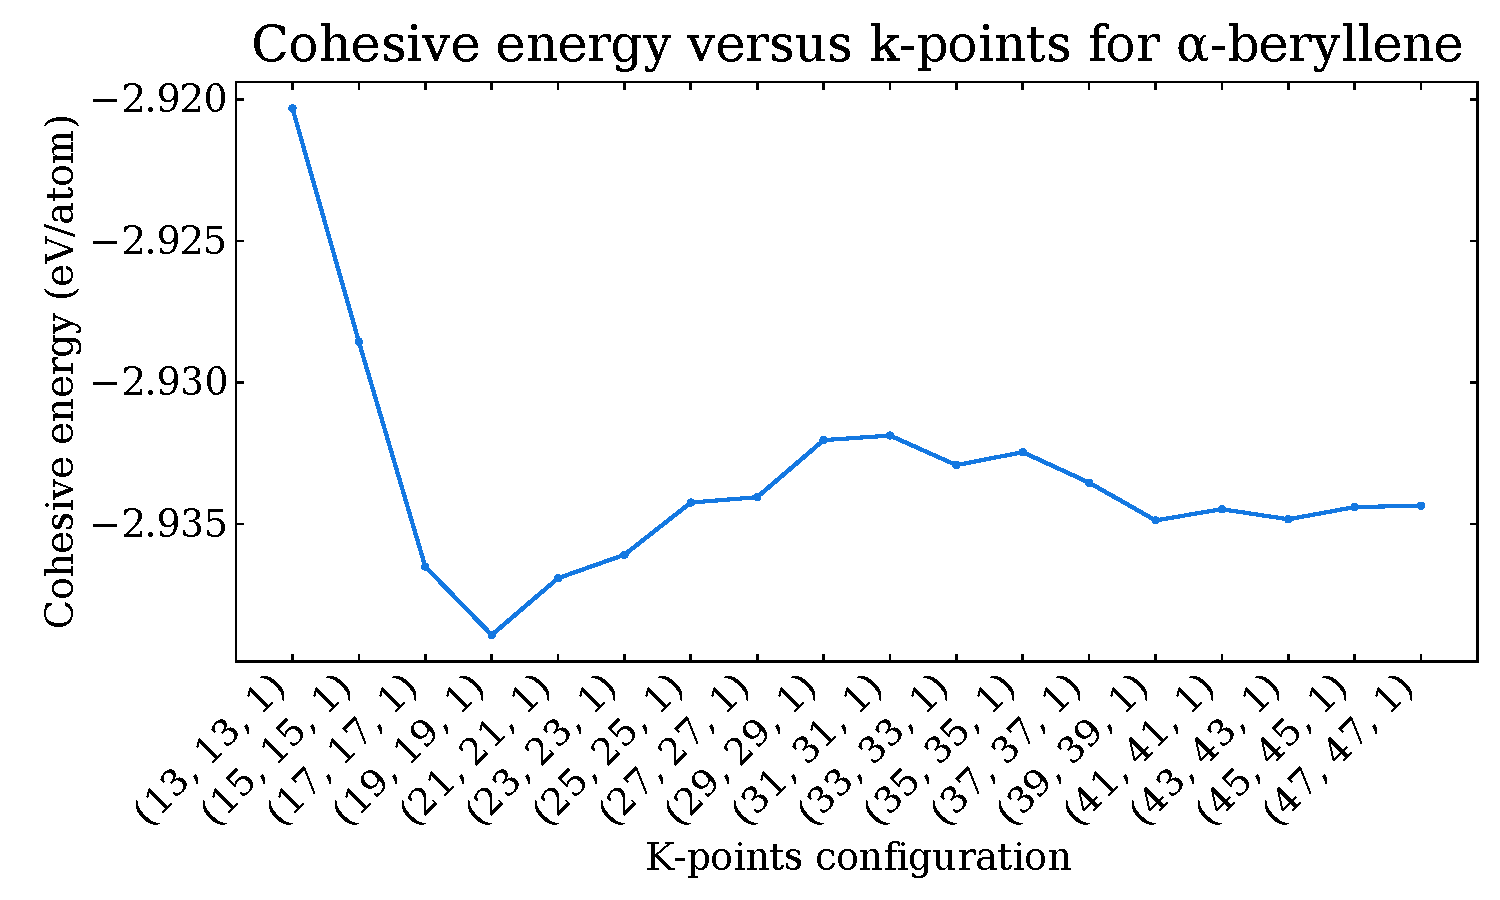
\includegraphics[width=0.40\linewidth]{figures_proj3/convergence_cohesive_kpoints_alpha-beryllene_thesis.pdf}\\
    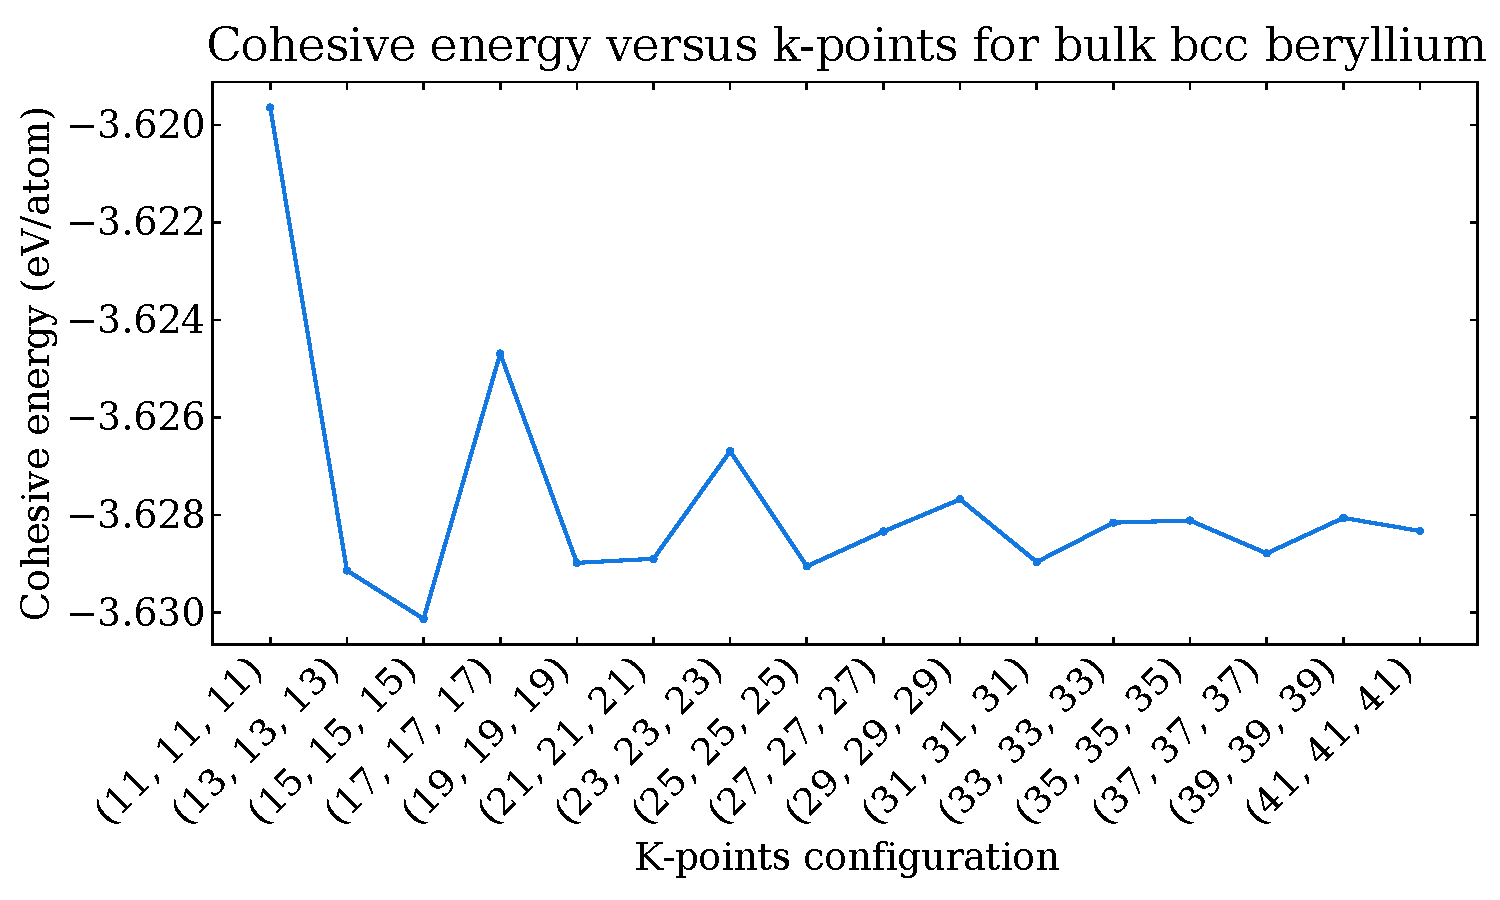
\includegraphics[width=0.40\linewidth]{figures_proj3/convergence_cohesive_kpoints_bcc-beryllium_thesis.pdf}&
    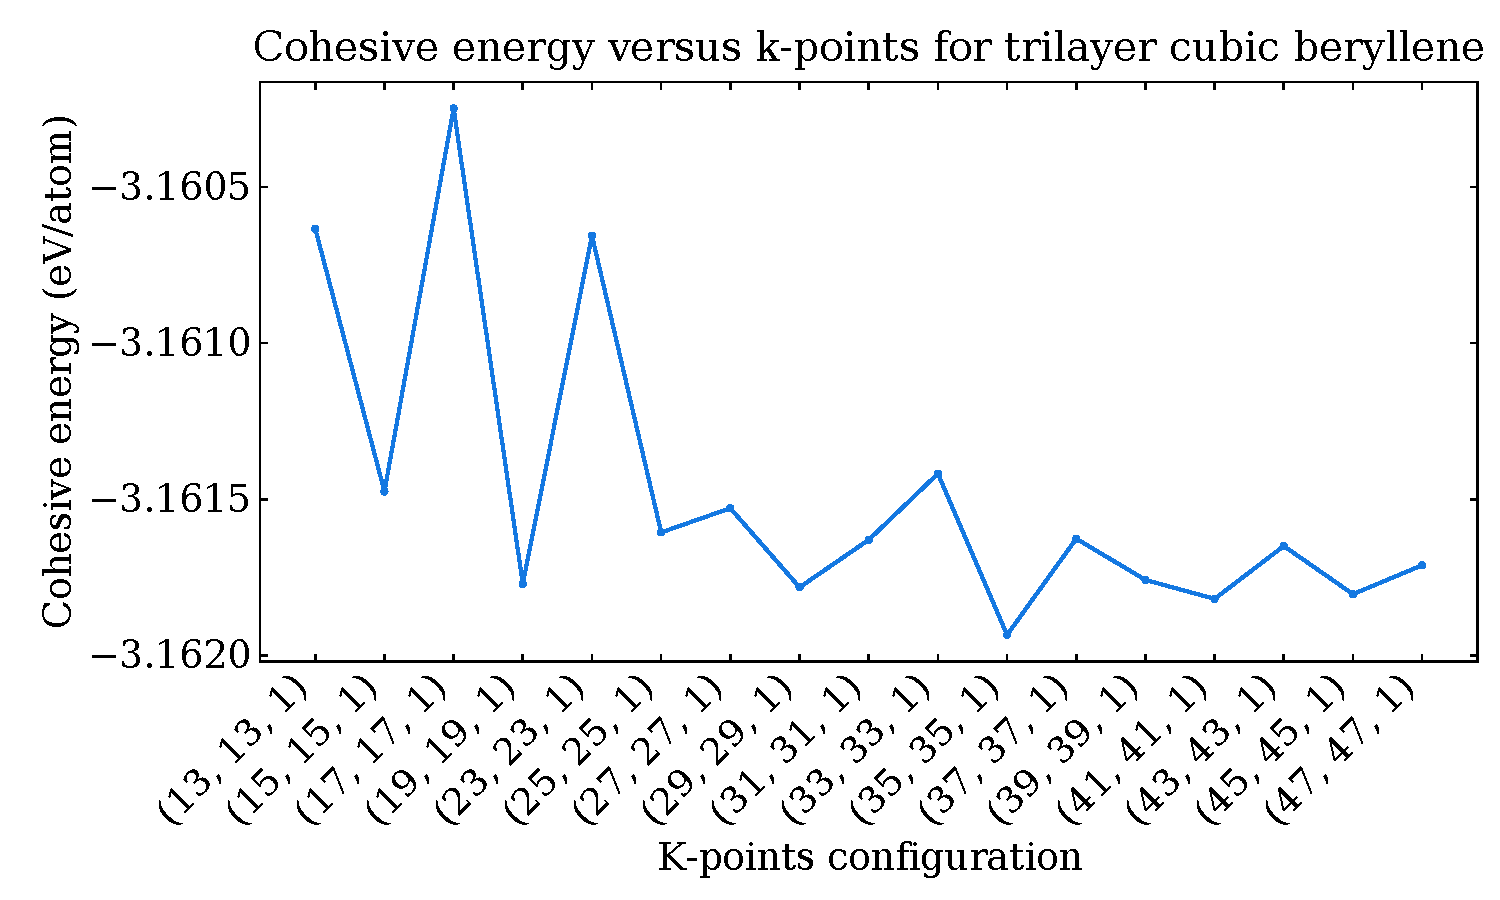
\includegraphics[width=0.40\linewidth]{figures_proj3/convergence_cohesive_kpoints_cubic-beryllene-trilayer_thesis.pdf}
\end{tabular}
\caption{Cohesive energy as a function of the k-point mesh for bulk hcp beryllium, $\alpha$-beryllene, bulk bcc beryllium, and trilayer cubic beryllene.}
\label{fig:proj3_cohesive_energy_convergence}
\end{figure}

\begin{figure}[!htbp]
\centering
\begin{tabular}{@{}cc@{}}
    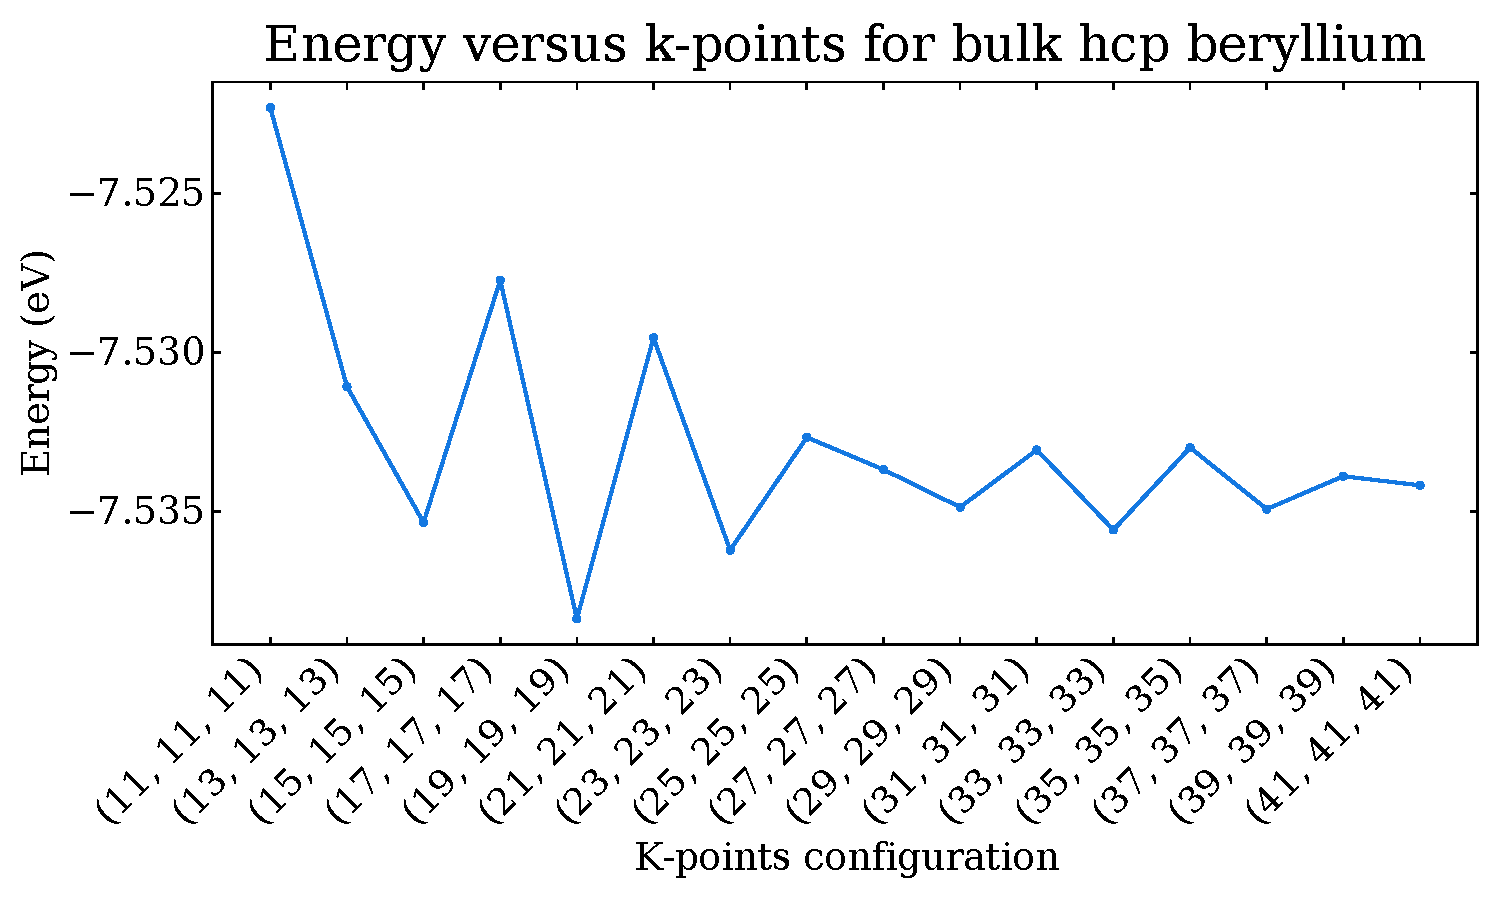
\includegraphics[width=0.40\linewidth]{figures_proj3/convergence_energy_kpoints_hcp-beryllium_thesis.pdf}&
    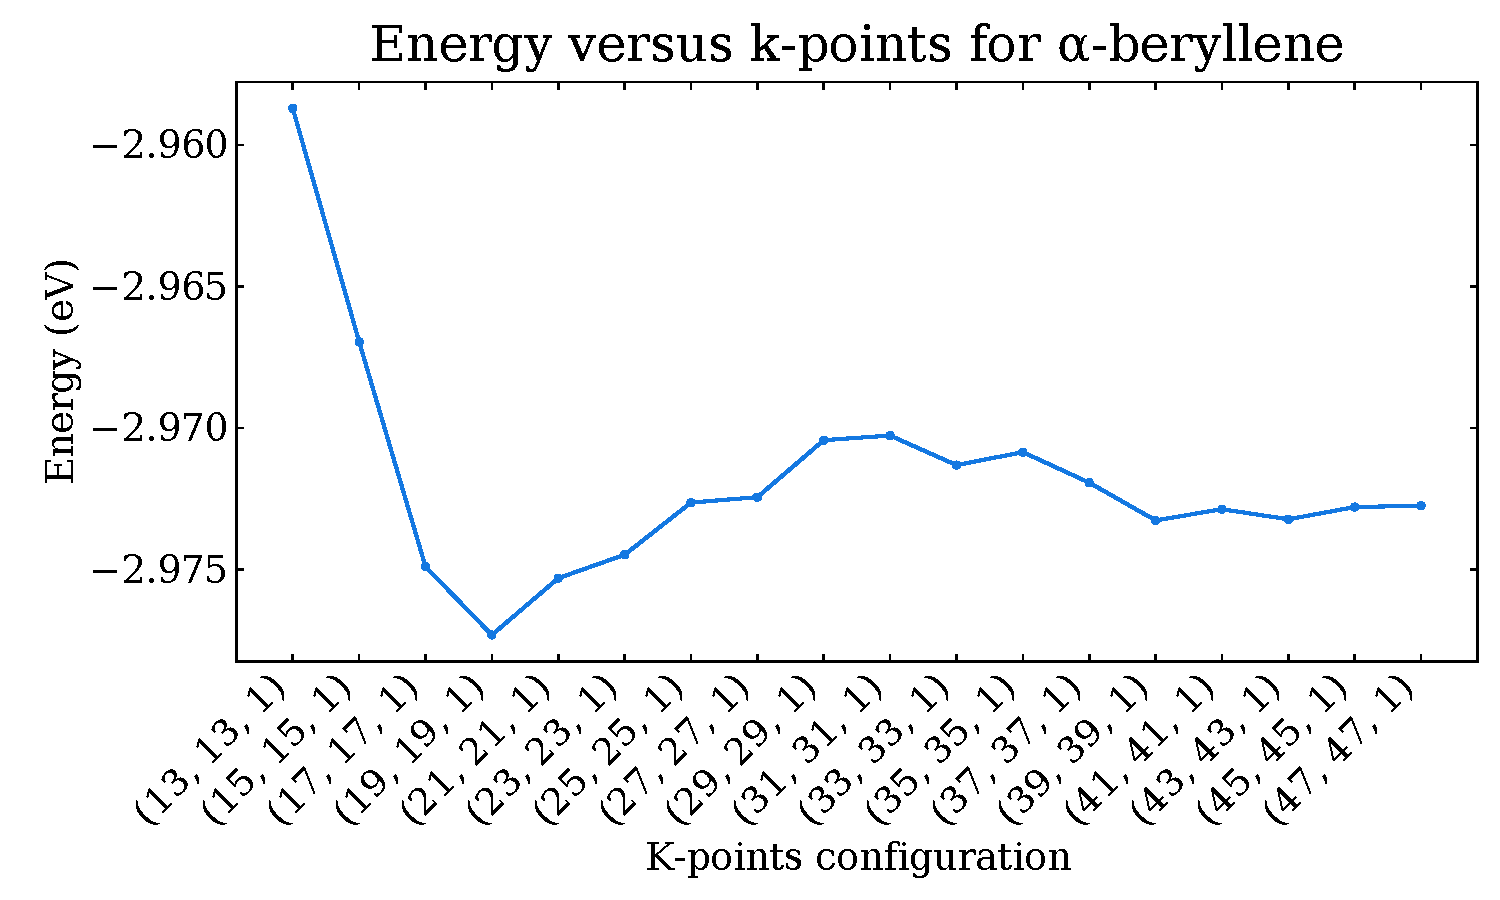
\includegraphics[width=0.40\linewidth]{figures_proj3/convergence_energy_kpoints_alpha-beryllene_thesis.pdf}\\
    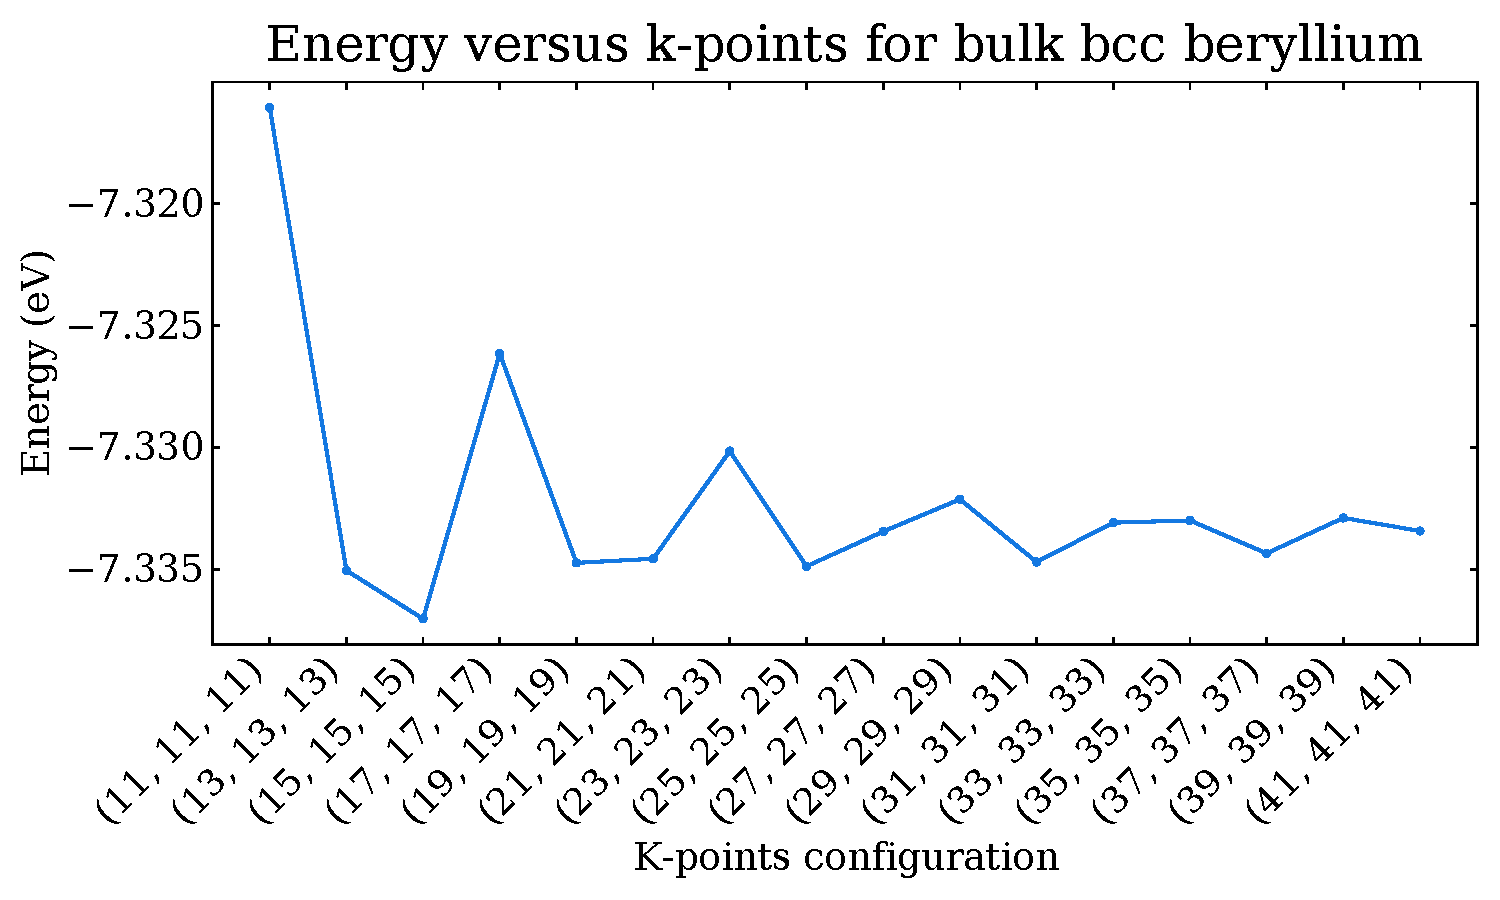
\includegraphics[width=0.40\linewidth]{figures_proj3/convergence_energy_kpoints_bcc-beryllium_thesis.pdf}&
    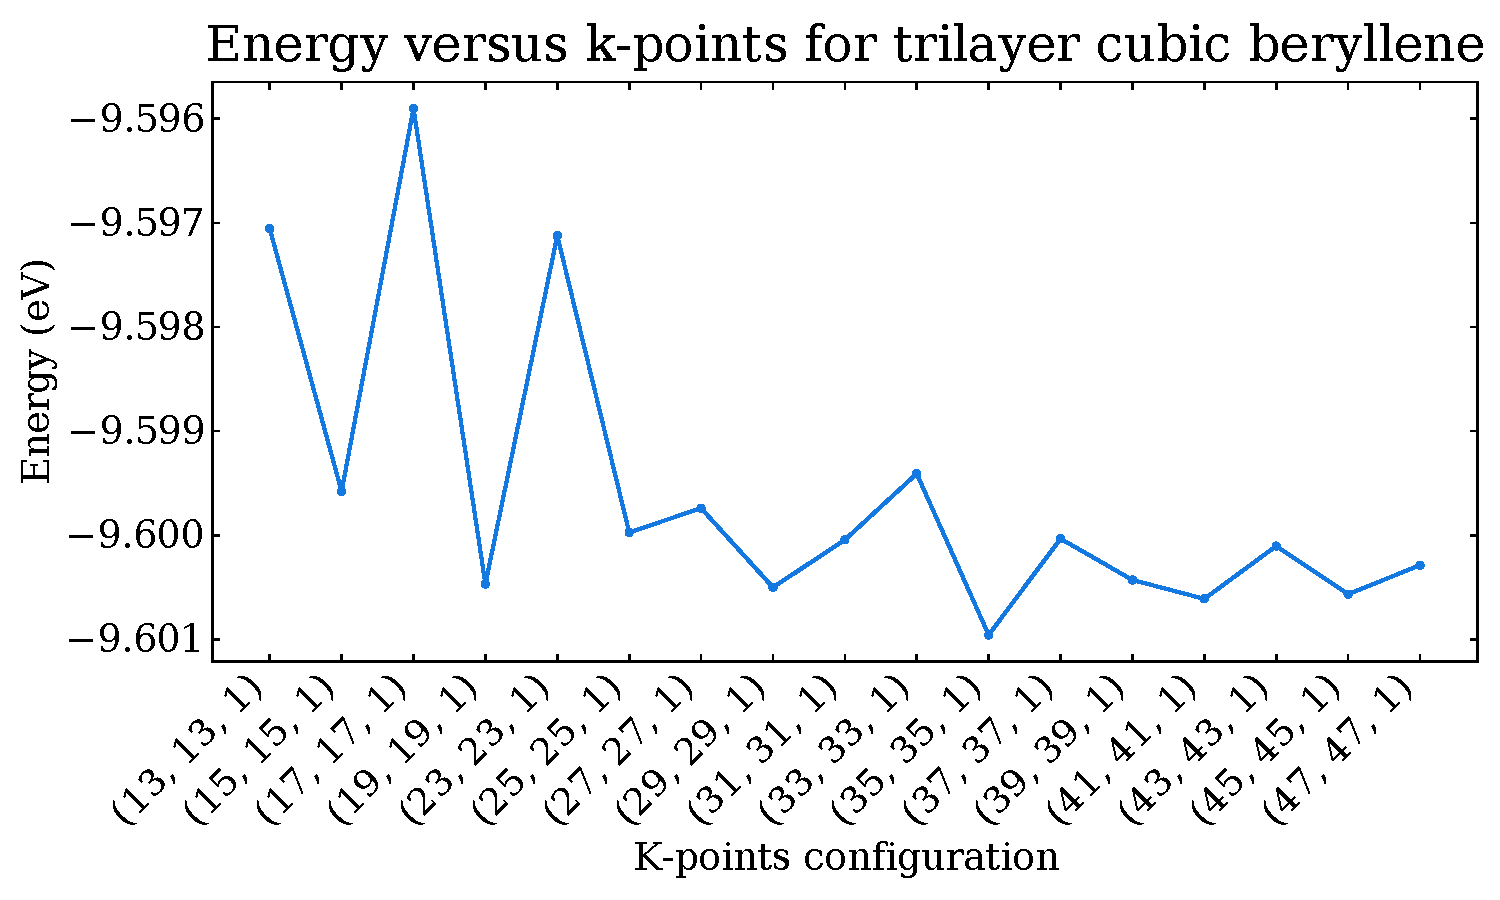
\includegraphics[width=0.40\linewidth]{figures_proj3/convergence_energy_kpoints_cubic-beryllene-trilayer_thesis.pdf}
\end{tabular}
\caption{Total energy as a function of the k-point mesh for bulk hcp beryllium, $\alpha$-beryllene, bulk bcc beryllium, and trilayer cubic beryllene.}
\label{fig:proj3_total_energy_convergence}
\end{figure}

\subsection*{Optical-calculation parameters}

The dielectric function and the derived optical observables are introduced in chapter~\ref{cha:fundamentals_b},
especially section~\ref{sec:from_dielectric_function_to_optical_properties},
and the optical volume normalization is given in equation~\eqref{optical_volume_normalization_2d}.
Therefore, we do not repeat these formula definitions here.
The structure thicknesses and the numbers of bands used in the optical calculations are specified below.

The effective thicknesses $d_{\mathrm{2D}}$ used in the optical volume normalization are
\qty{3.960}{\angstrom} for pristine $\alpha$-beryllene,
\qty{5.869}{\angstrom} for pristine $\beta$-beryllene,
\qty{6.966}{\angstrom} for trilayer cubic beryllene,
\qty{3.145}{\angstrom} for 2H-$\alpha$-beryllene,
\qty{5.524}{\angstrom} for 1H-$\beta$-beryllene,
and \qty{5.193}{\angstrom} for 2H-$\beta$-beryllene.
We assign $d_{\mathrm{2D}}$ as the separation of the outermost atomic centres along the surface normal,
plus the radii of the atoms at those two surfaces.
These radii are \qty{1.98}{\angstrom} for Be and \qty{0.70}{\angstrom} for H.
The relaxed coordinates are converted to Cartesian lengths with periodic wrapping removed.
The same optical volume normalization is applied to the $xx$, $yy$, and $zz$ components.
The absolute effective response depends on this thickness convention.
The endpoint-radius contribution is Be+Be for pristine structures, H+H for double-sided termination, and Be+H for single-sided termination.
Consequently, the assigned thickness of 2H-$\alpha$-beryllene is smaller than that of pristine $\alpha$-beryllene.
Unrounded structure-derived values are used in all calculations.
The actual total numbers of bands are 140 for each hydrogen-functionalized structure,
133 for pristine $\alpha$-beryllene and trilayer cubic beryllene,
128 for pristine $\beta$-beryllene,
70 for bulk bcc beryllium,
and 66 for bulk hcp beryllium.
These numbers include both occupied and unoccupied bands.
They can differ from the requested \texttt{NBANDS} because of parallel band allocation.

\subsection*{Dielectric-function convergence}

The convergence of the calculated dielectric function is examined with respect to the number of bands included in the calculation and the k-point mesh.
Figures~\ref{fig:proj3_hcp_dielectric_nbands_convergence}--\ref{fig:proj3_cubic_dielectric_kpoint_convergence}
show the corresponding tests for bulk hcp beryllium,
$\alpha$-beryllene, $\beta$-beryllene, bulk bcc beryllium,
and trilayer cubic beryllene.
The plots retain the full range of every curve within the displayed energy window.
In particular, the bulk hcp $45\times45\times45$ k-point calculation has a large low-energy dielectric response that is visible in figure~\ref{fig:proj3_hcp_dielectric_kpoint_convergence}.
These comparisons test the convergence of the interband response, and the complete low-frequency metallic response would also require an intraband treatment.
The selected reference is the final-parameter calculation,
so its k-point mesh and total band count can differ from those of the convergence series.

\begin{figure}[!htbp]
\centering
    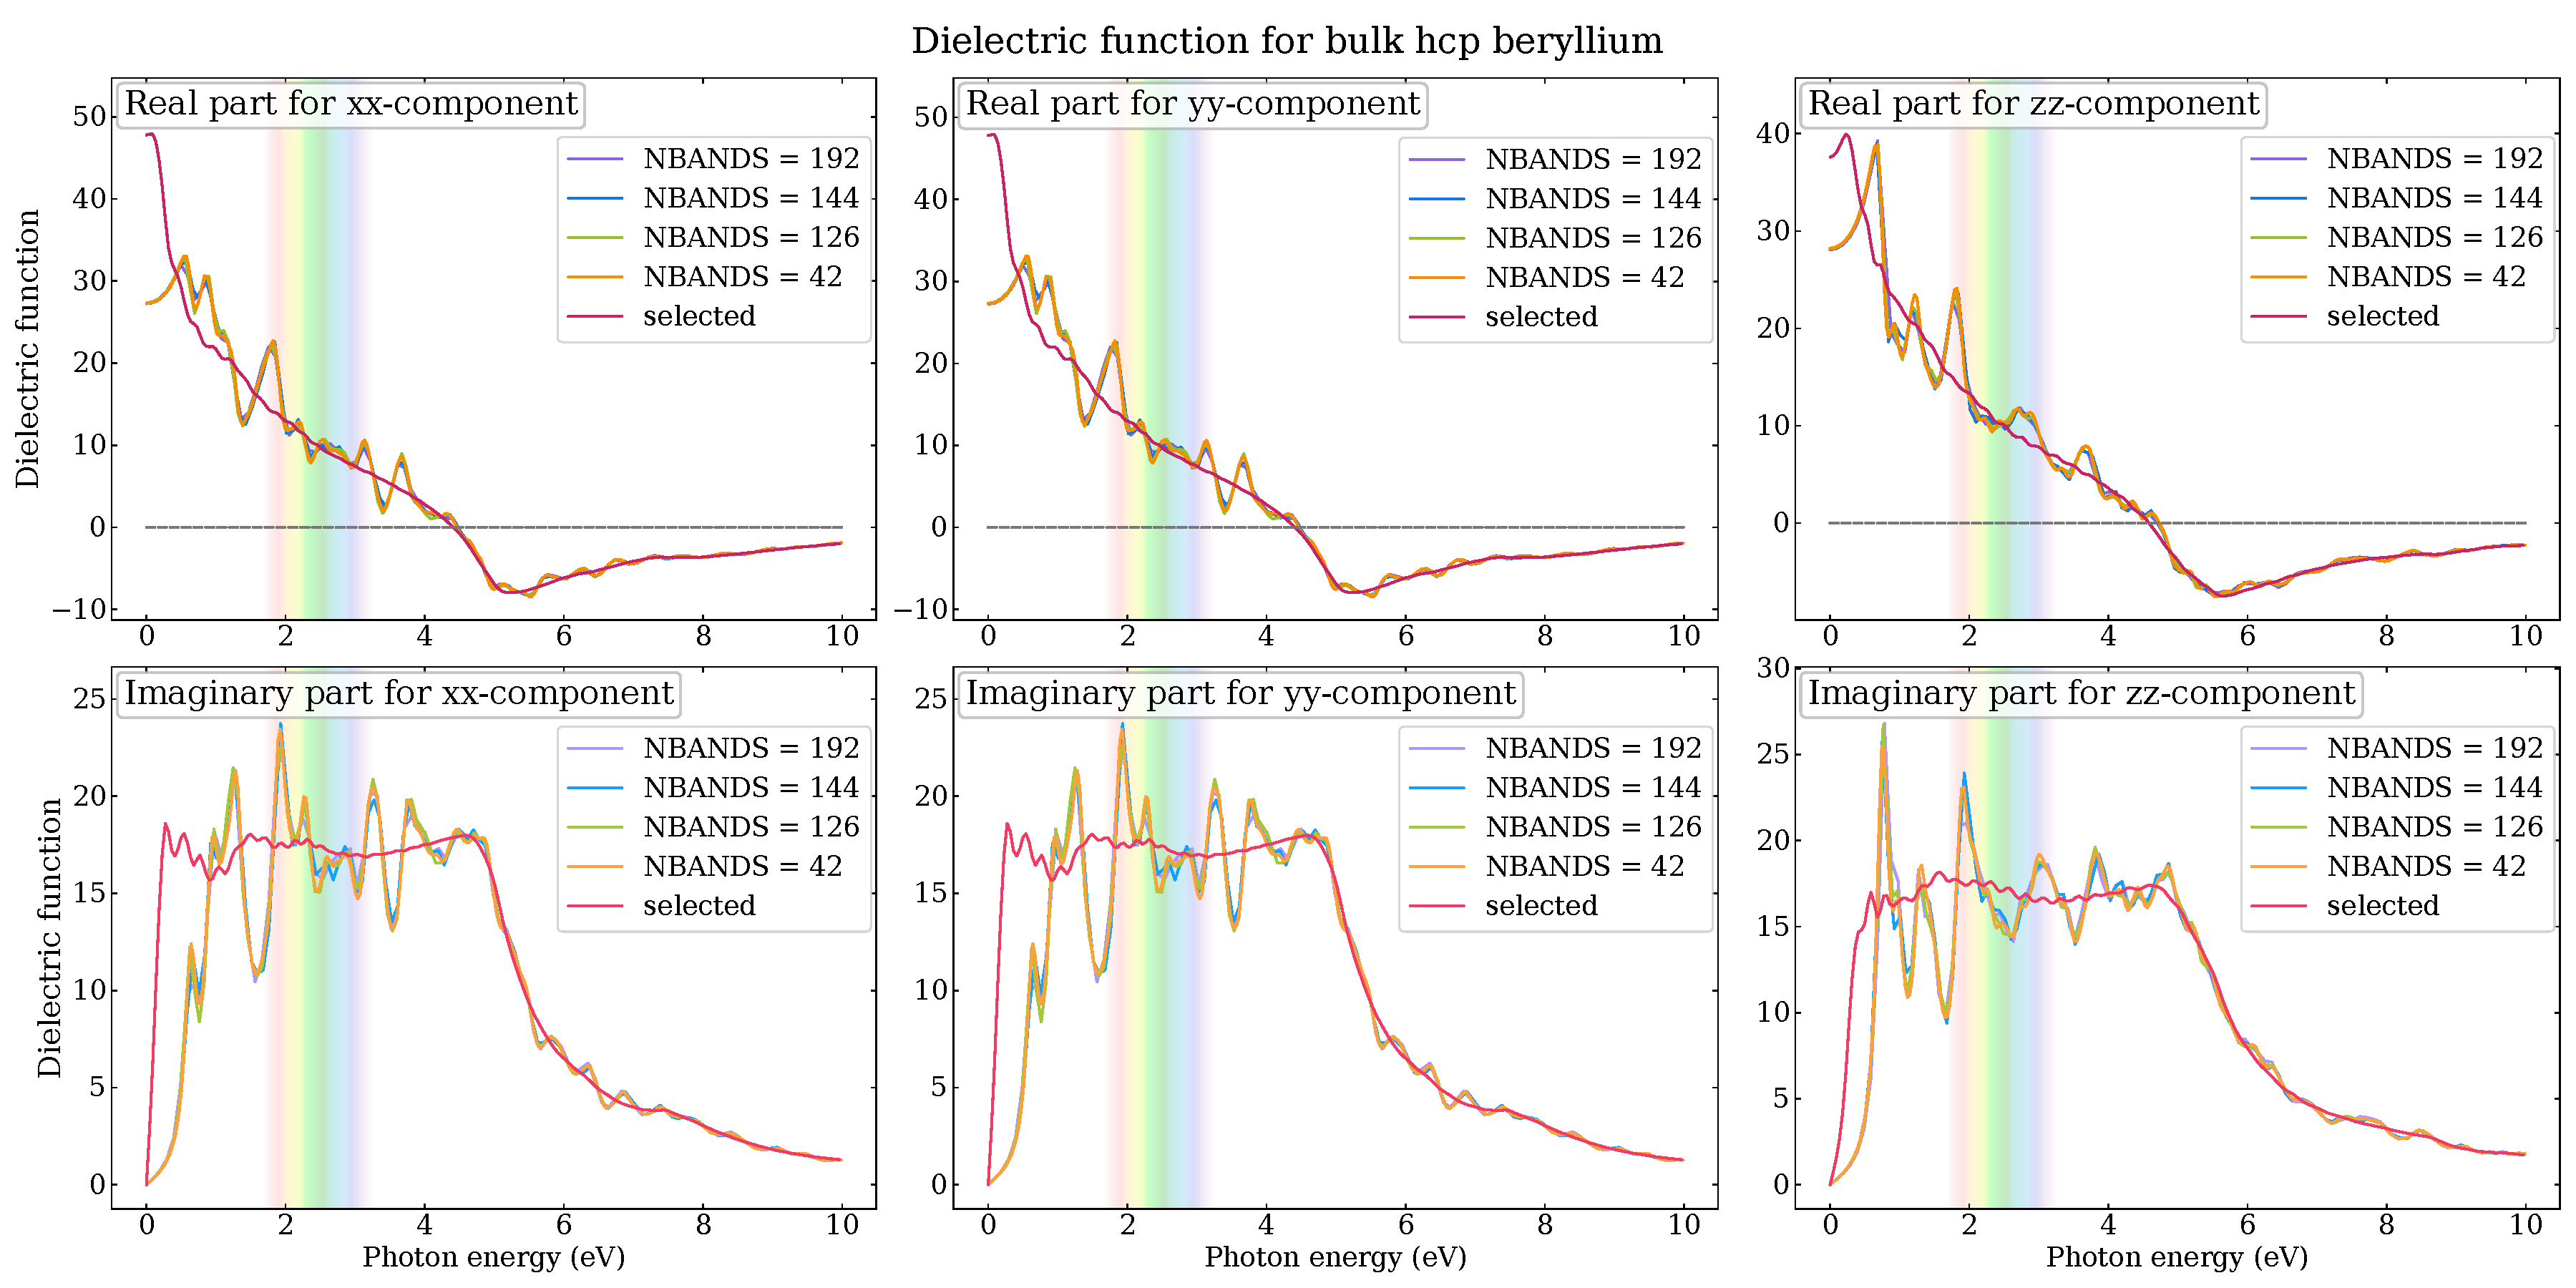
\includegraphics[width=1.0\linewidth]{figures_proj3/convergence_dielectric_nbands_hcp-beryllium_thesis.pdf}
\caption{Real and imaginary parts of the dielectric function for bulk hcp beryllium,
calculated with different total numbers of bands.}
\label{fig:proj3_hcp_dielectric_nbands_convergence}
\end{figure}

\begin{figure}[!htbp]
\centering
    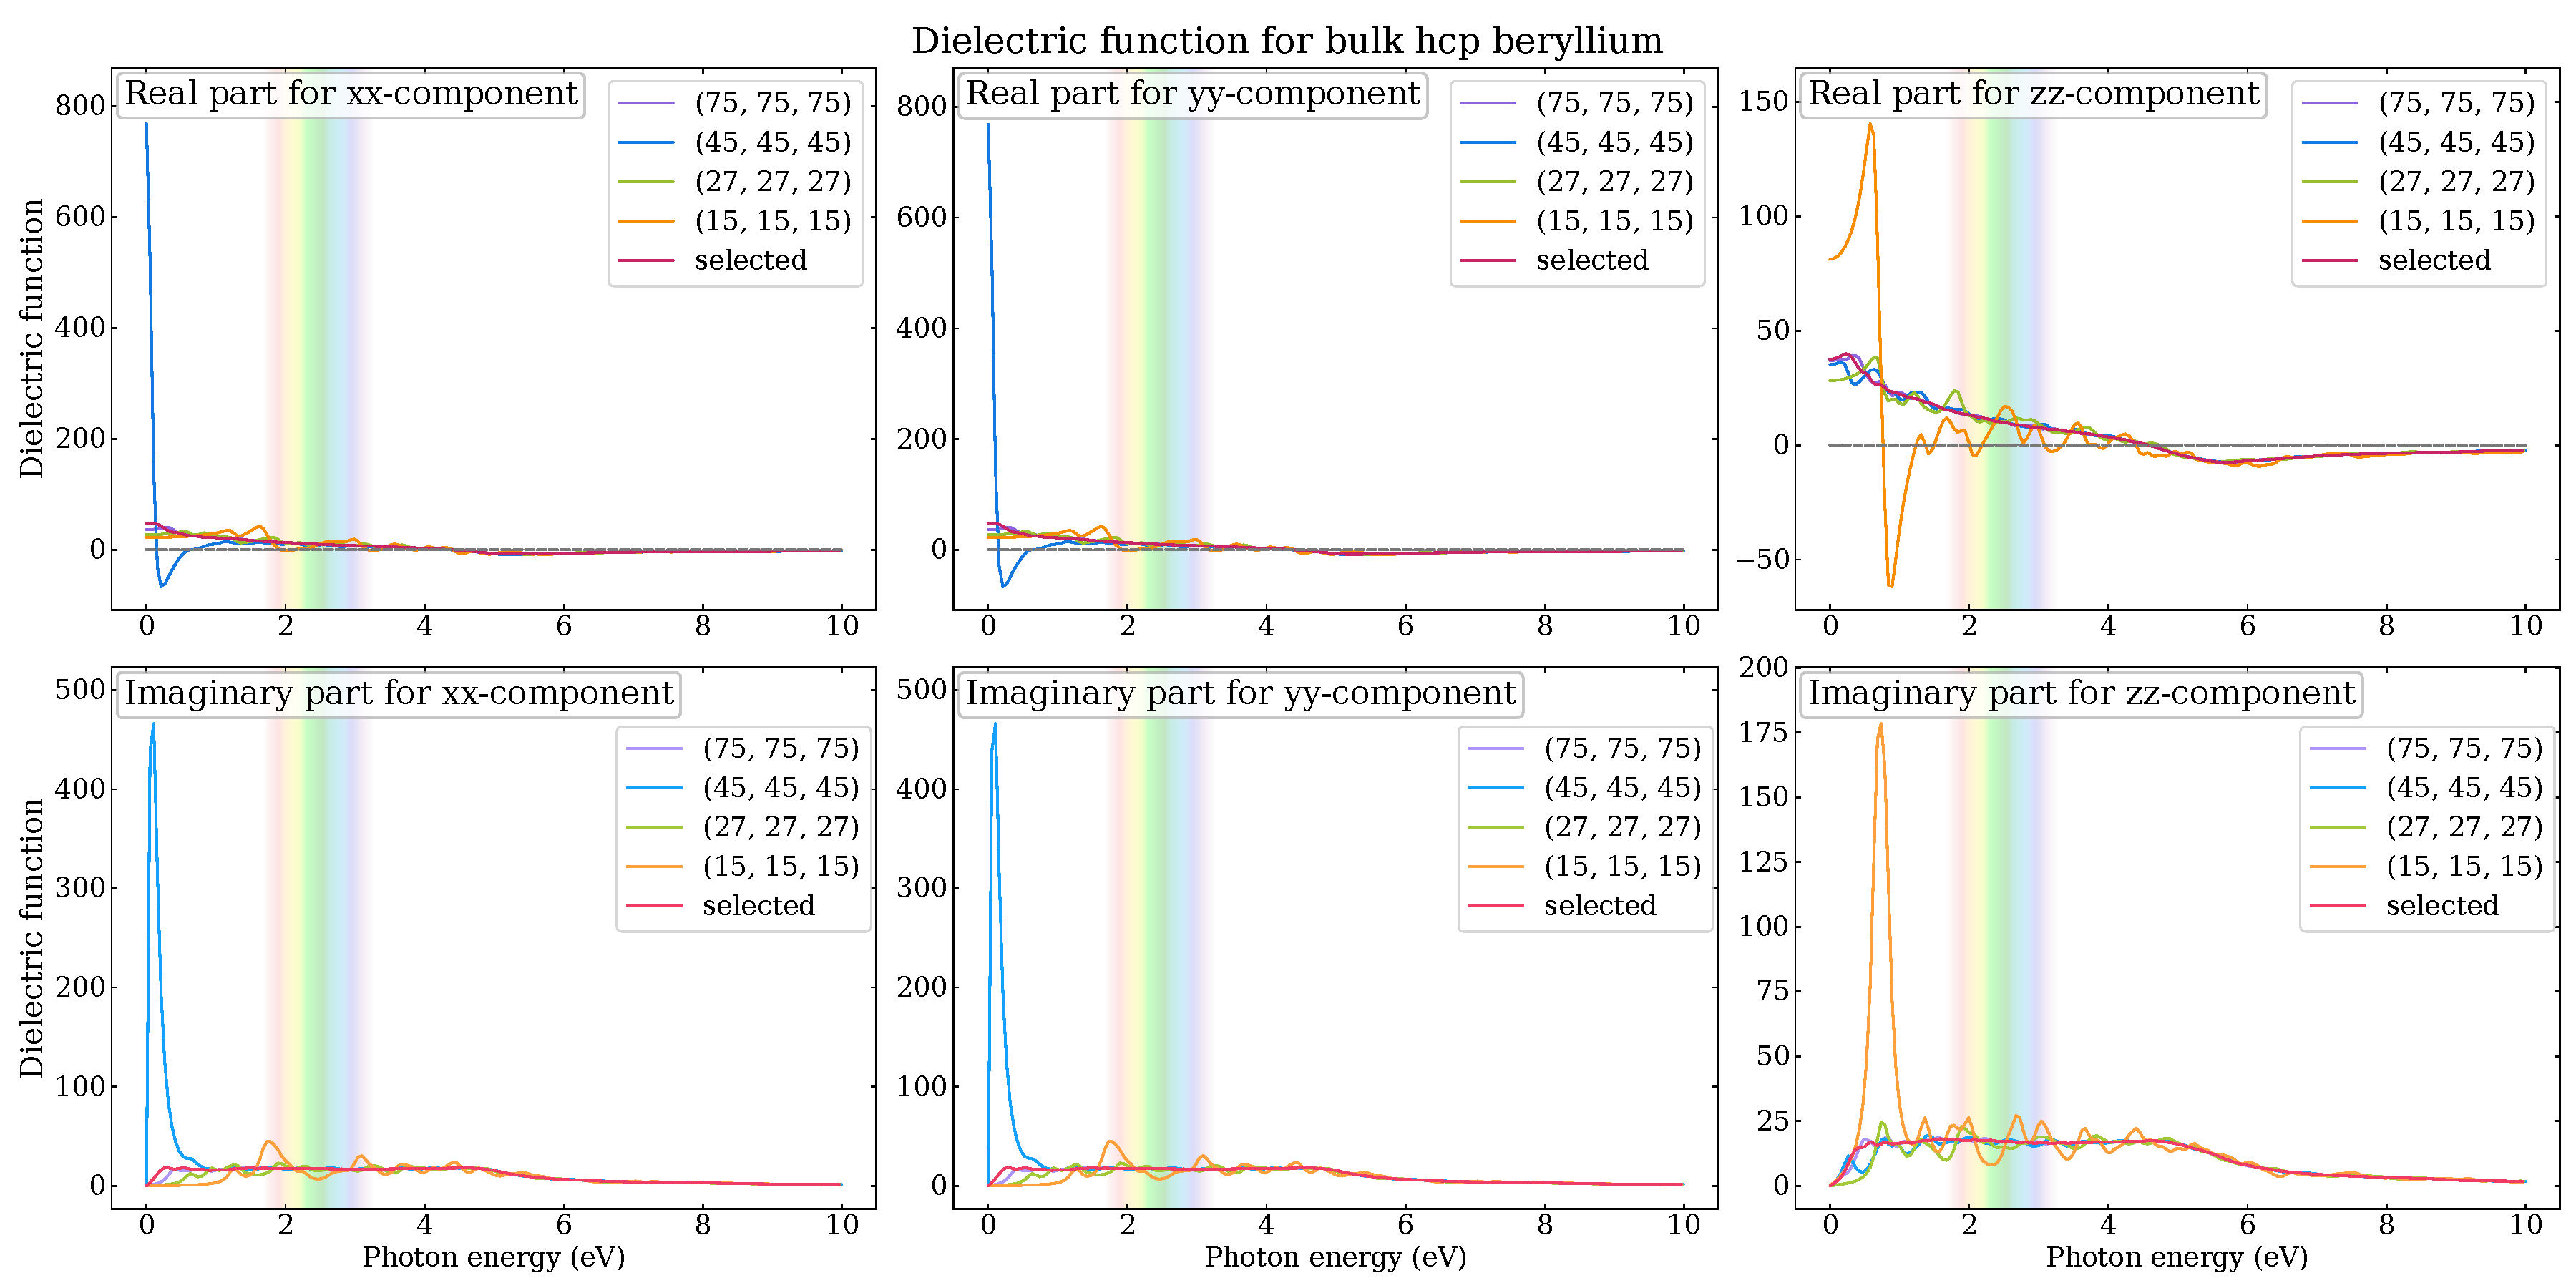
\includegraphics[width=1.0\linewidth]{figures_proj3/convergence_dielectric_kpoints_hcp-beryllium_thesis.pdf}
\caption{Real and imaginary parts of the dielectric function for bulk hcp beryllium,
calculated with different k-point meshes.}
\label{fig:proj3_hcp_dielectric_kpoint_convergence}
\end{figure}

\begin{figure}[!htbp]
\centering
    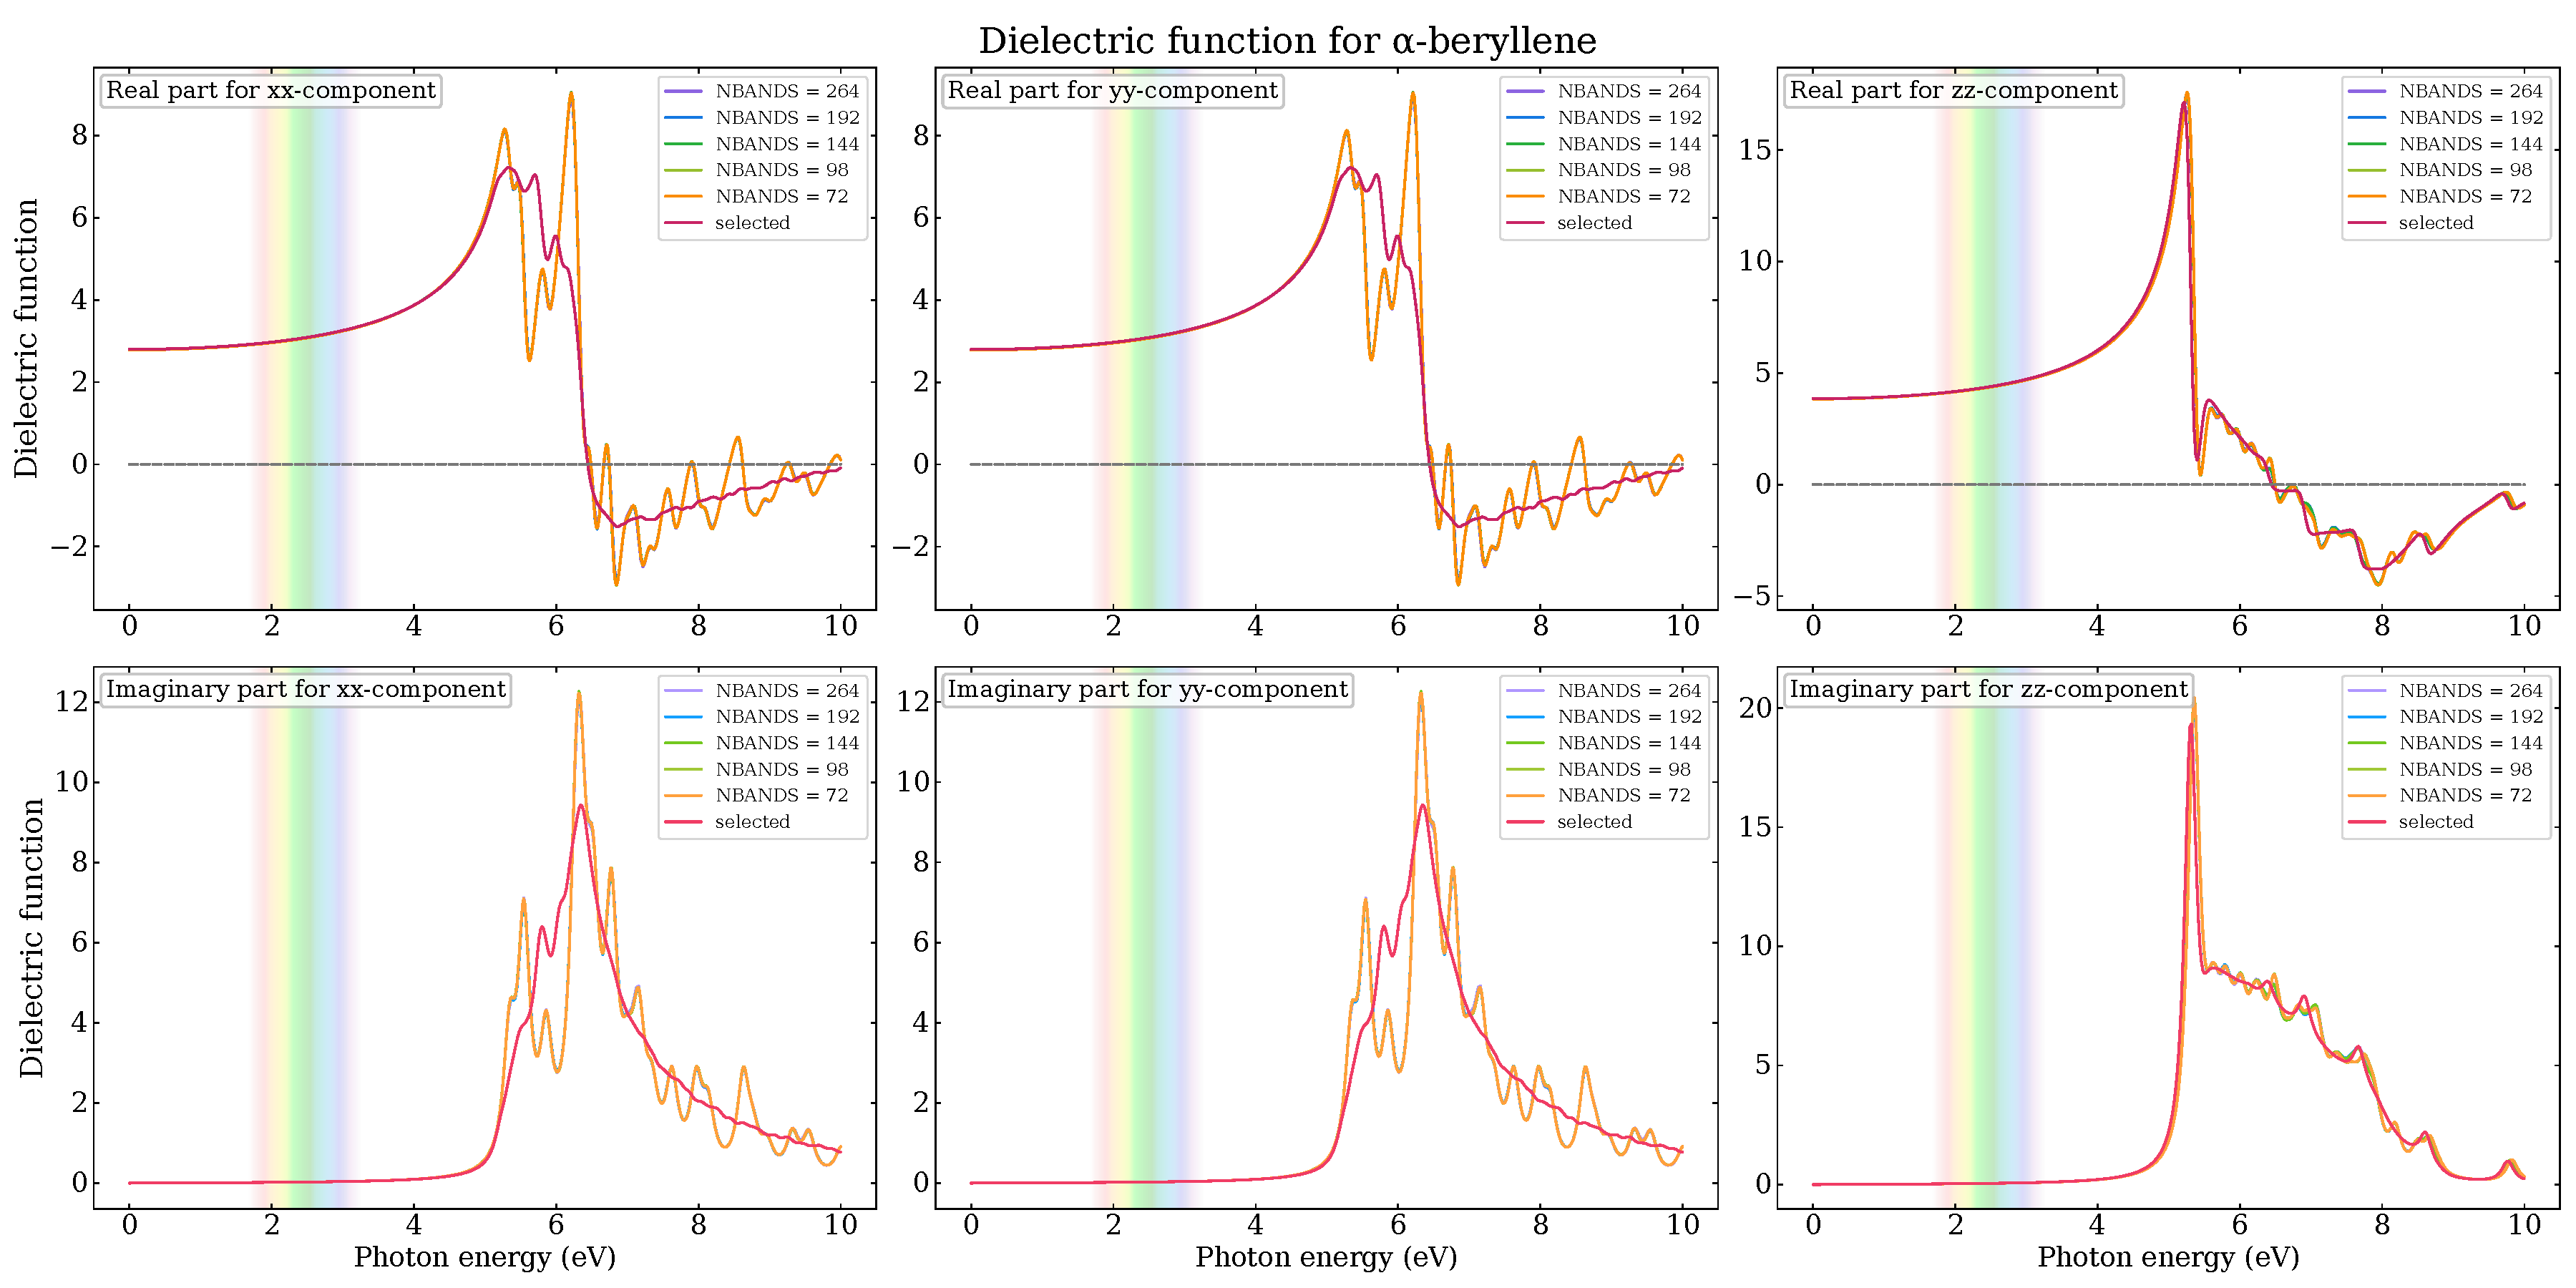
\includegraphics[width=1.0\linewidth]{figures_proj3/convergence_dielectric_nbands_alpha-beryllene_thesis.pdf}
\caption{Real and imaginary parts of the dielectric function for $\alpha$-beryllene,
calculated with different total numbers of bands.}
\label{fig:proj3_alpha_dielectric_nbands_convergence}
\end{figure}

\begin{figure}[!htbp]
\centering
    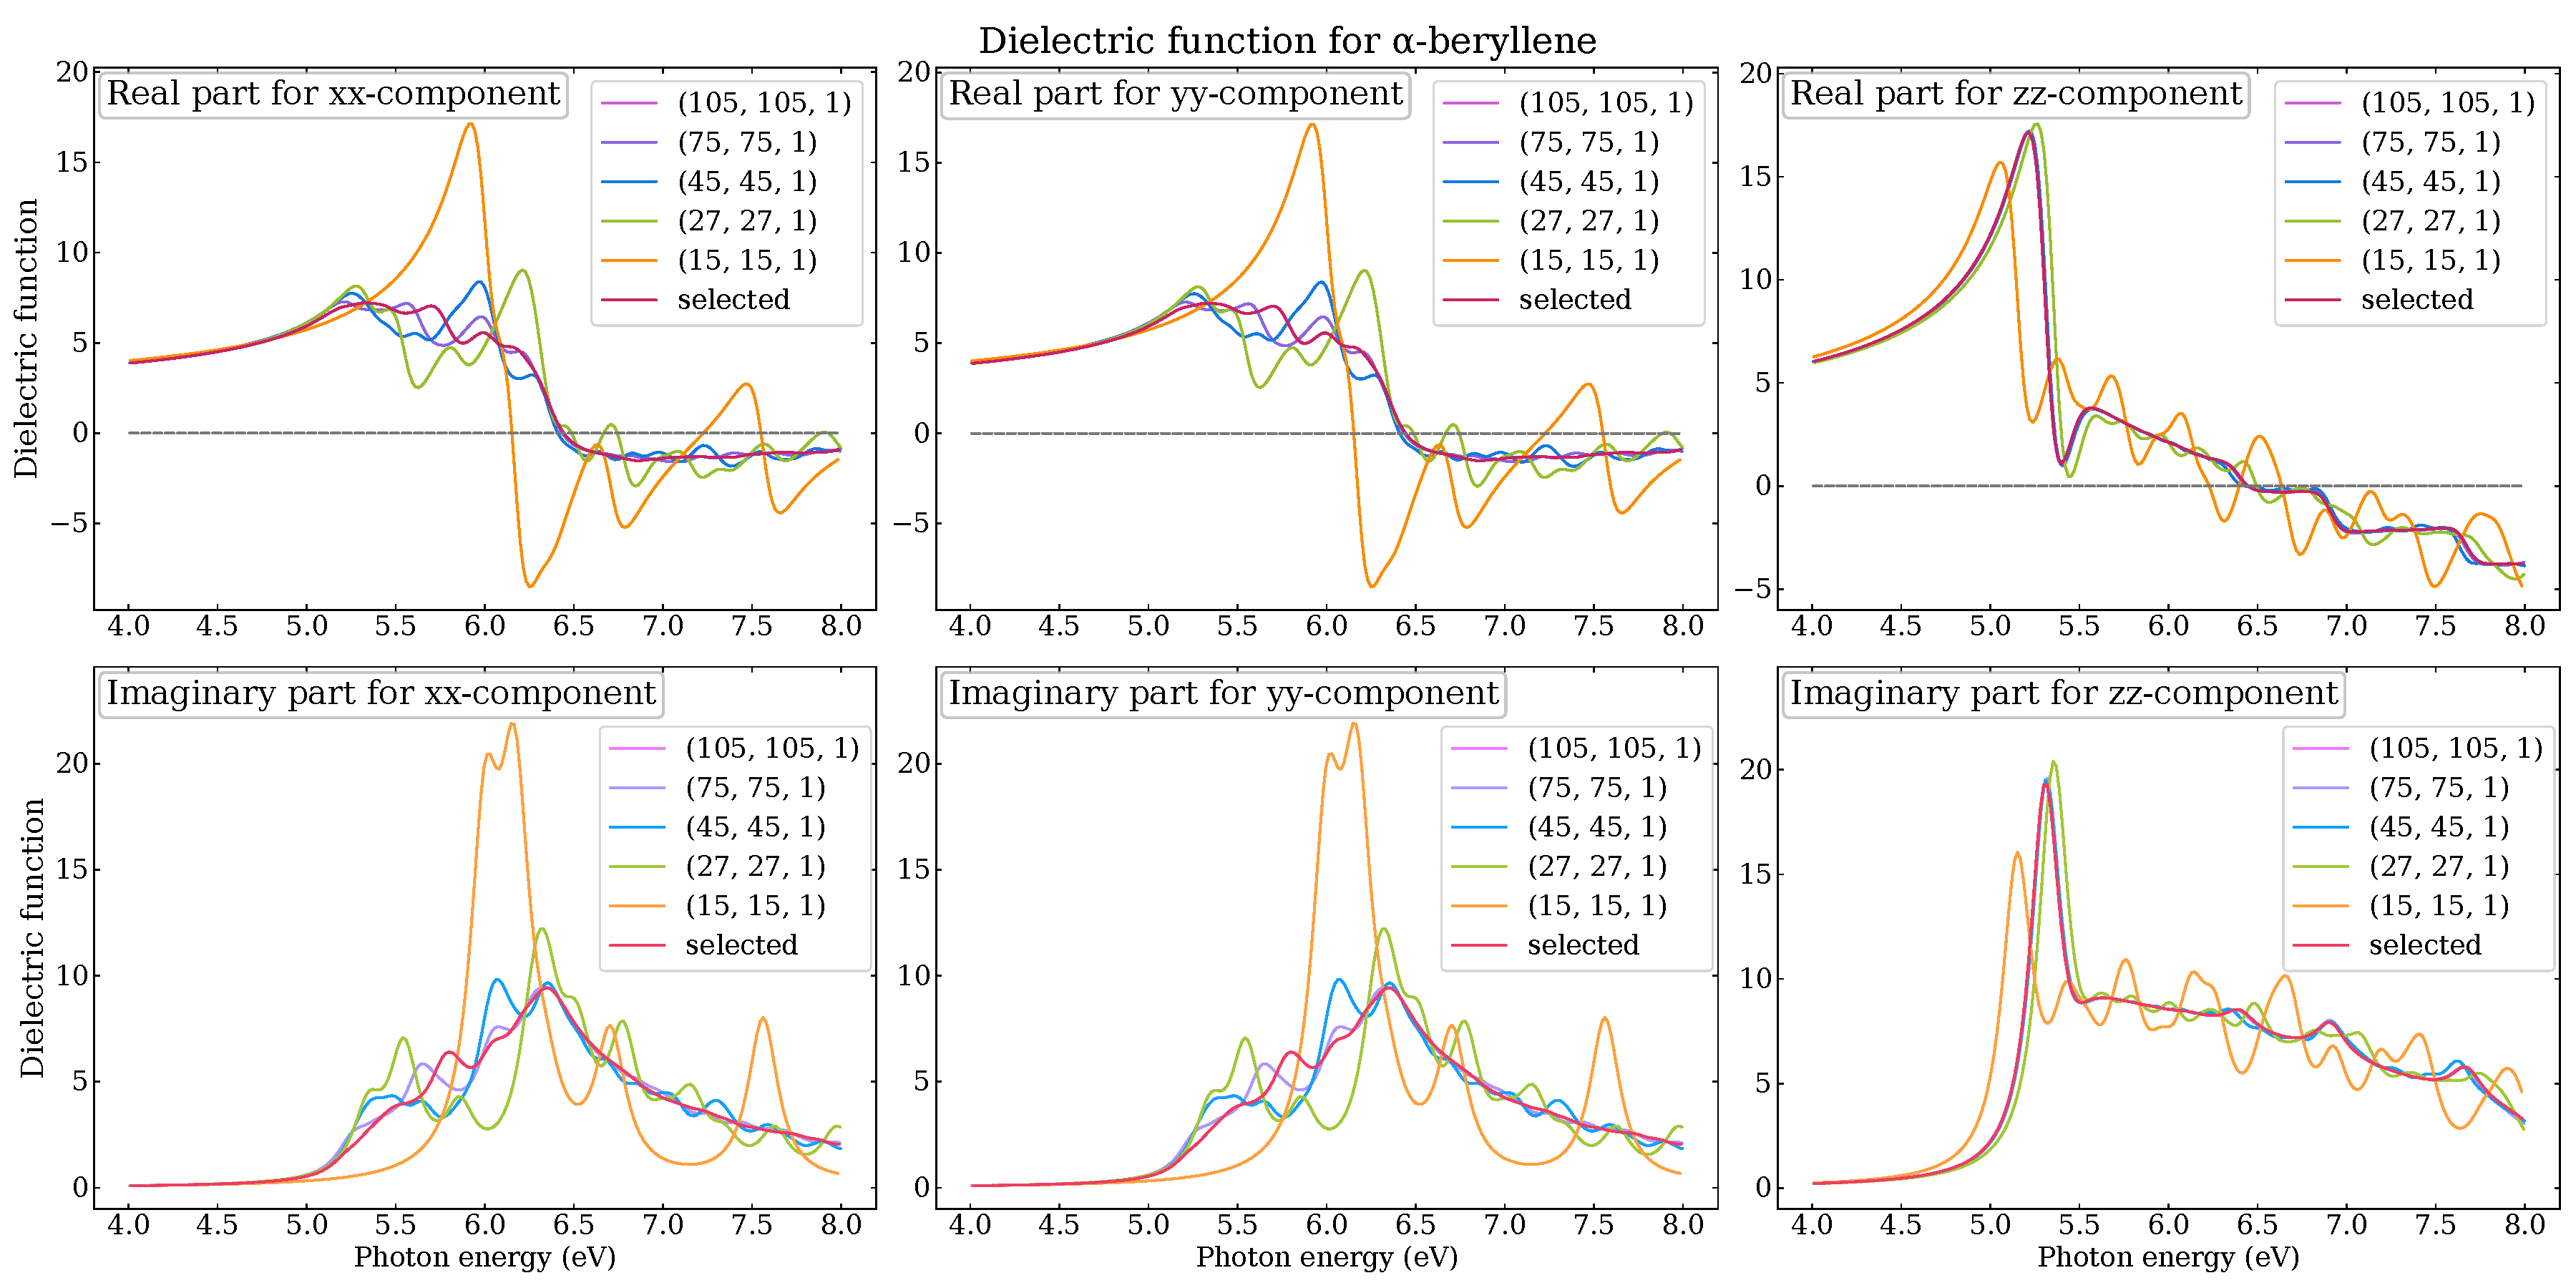
\includegraphics[width=1.0\linewidth]{figures_proj3/convergence_dielectric_kpoints_alpha-beryllene_thesis.pdf}
\caption{Real and imaginary parts of the dielectric function for $\alpha$-beryllene,
calculated with different k-point meshes.}
\label{fig:proj3_alpha_dielectric_kpoint_convergence}
\end{figure}

\begin{figure}[!htbp]
\centering
    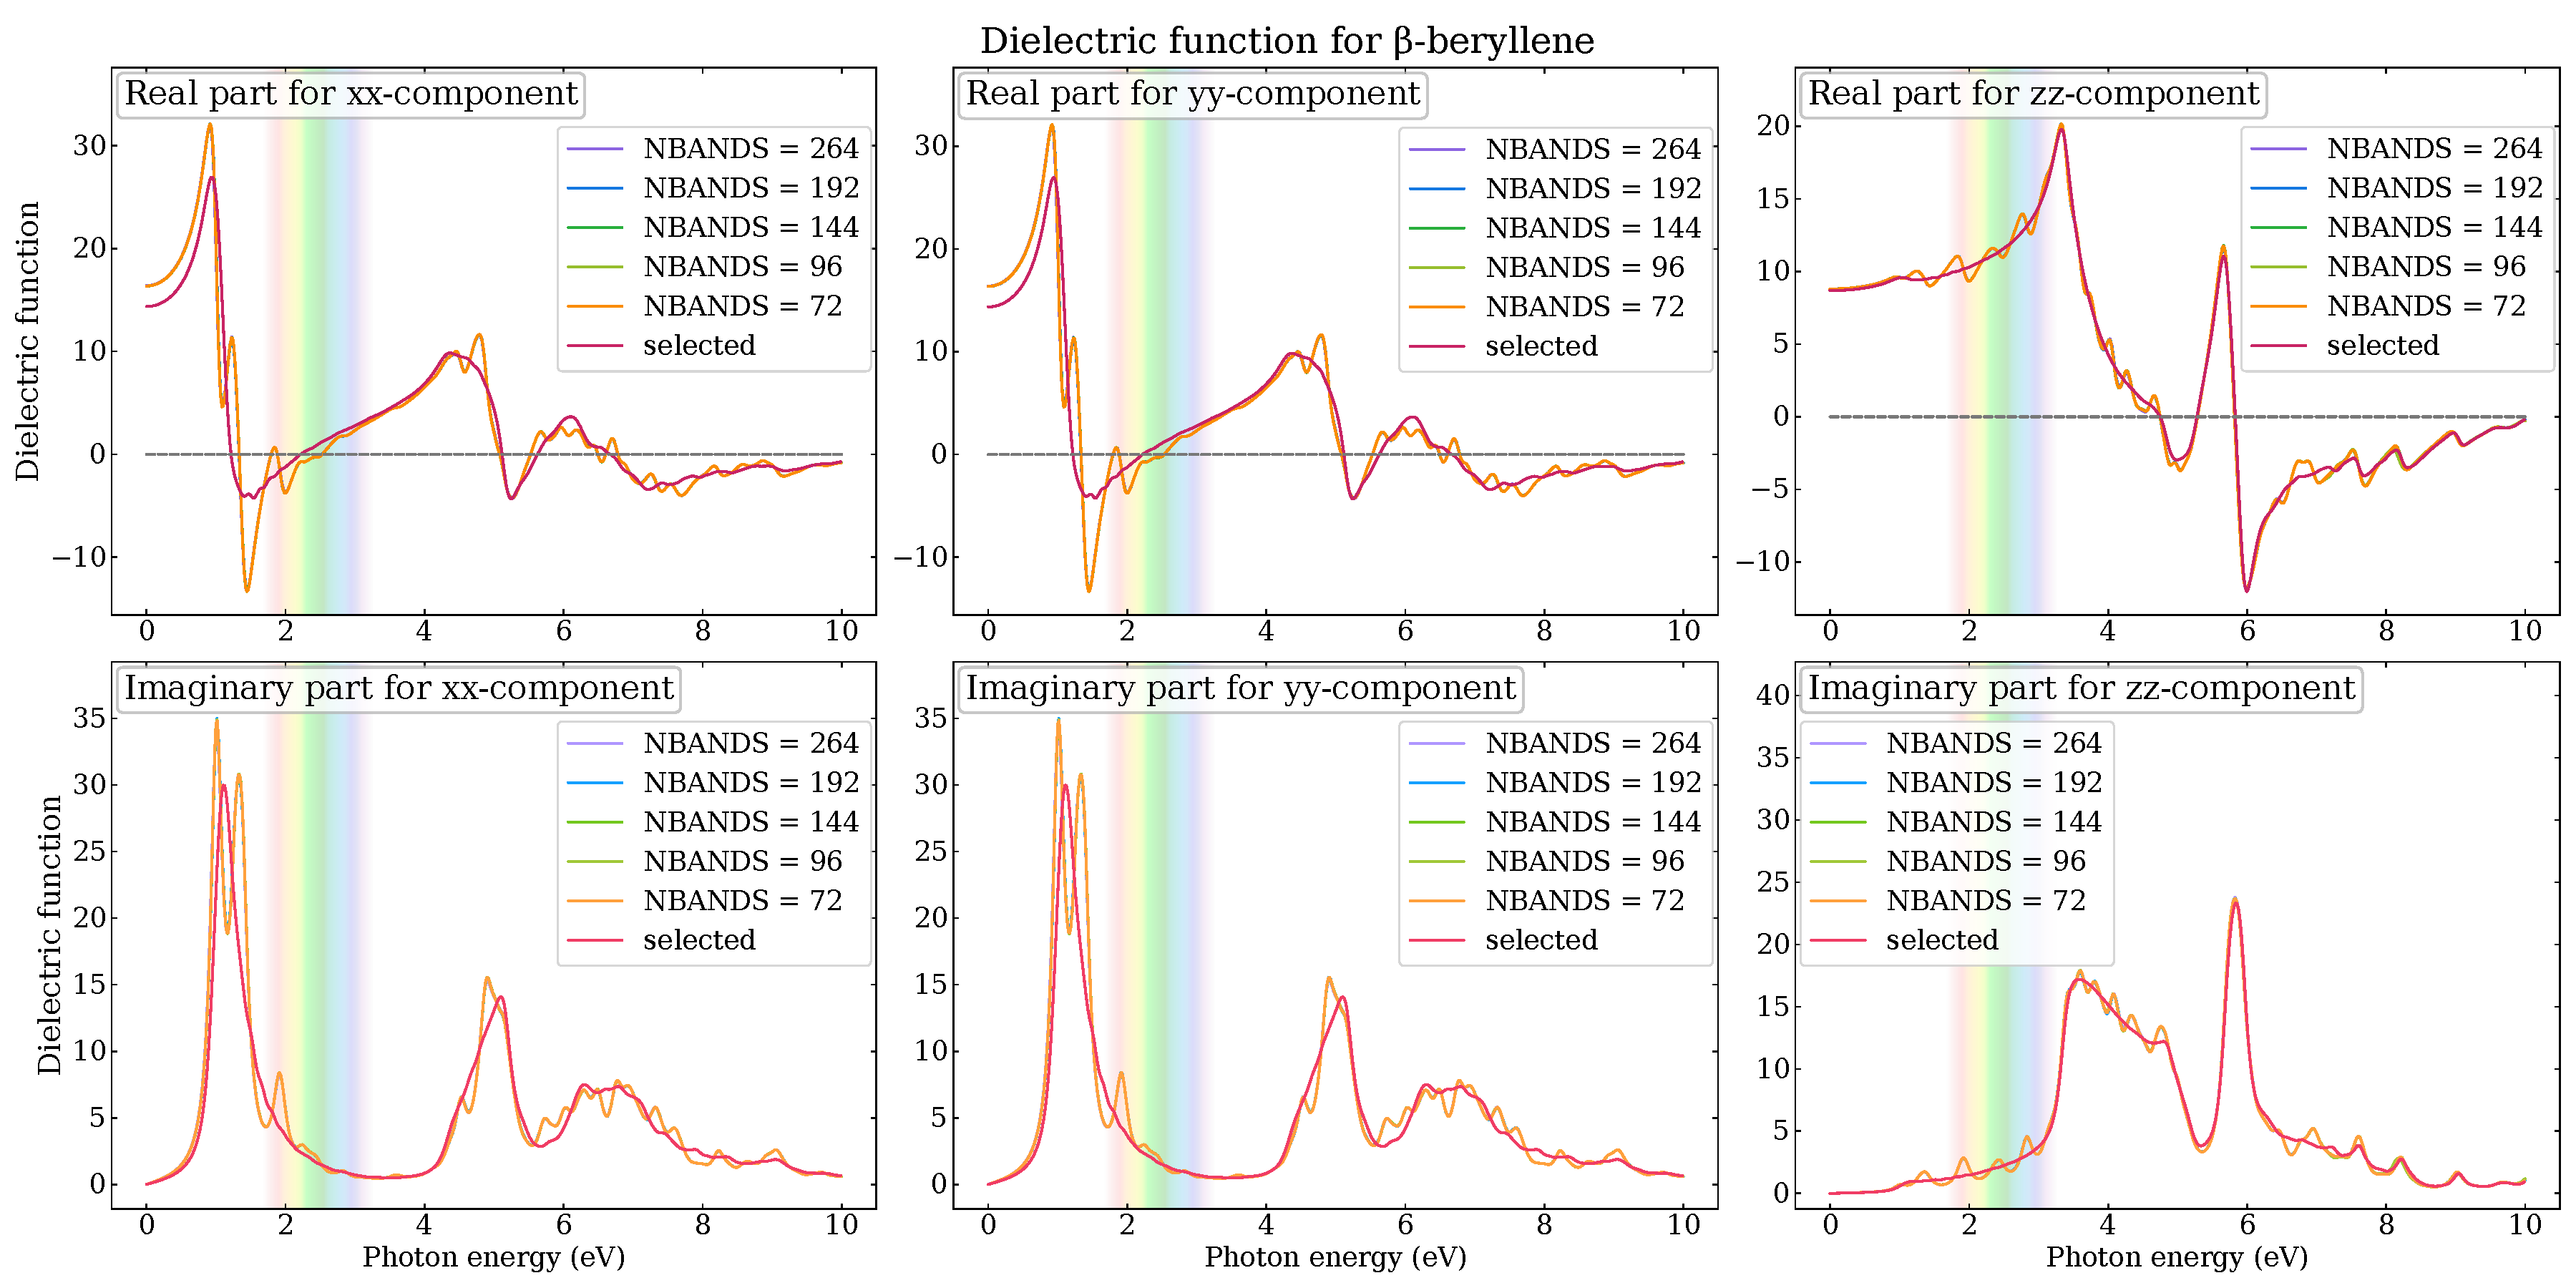
\includegraphics[width=1.0\linewidth]{figures_proj3/convergence_dielectric_nbands_beta-beryllene_thesis.pdf}
\caption{Real and imaginary parts of the dielectric function for $\beta$-beryllene,
calculated with different total numbers of bands.}
\label{fig:proj3_beta_dielectric_nbands_convergence}
\end{figure}

\begin{figure}[!htbp]
\centering
    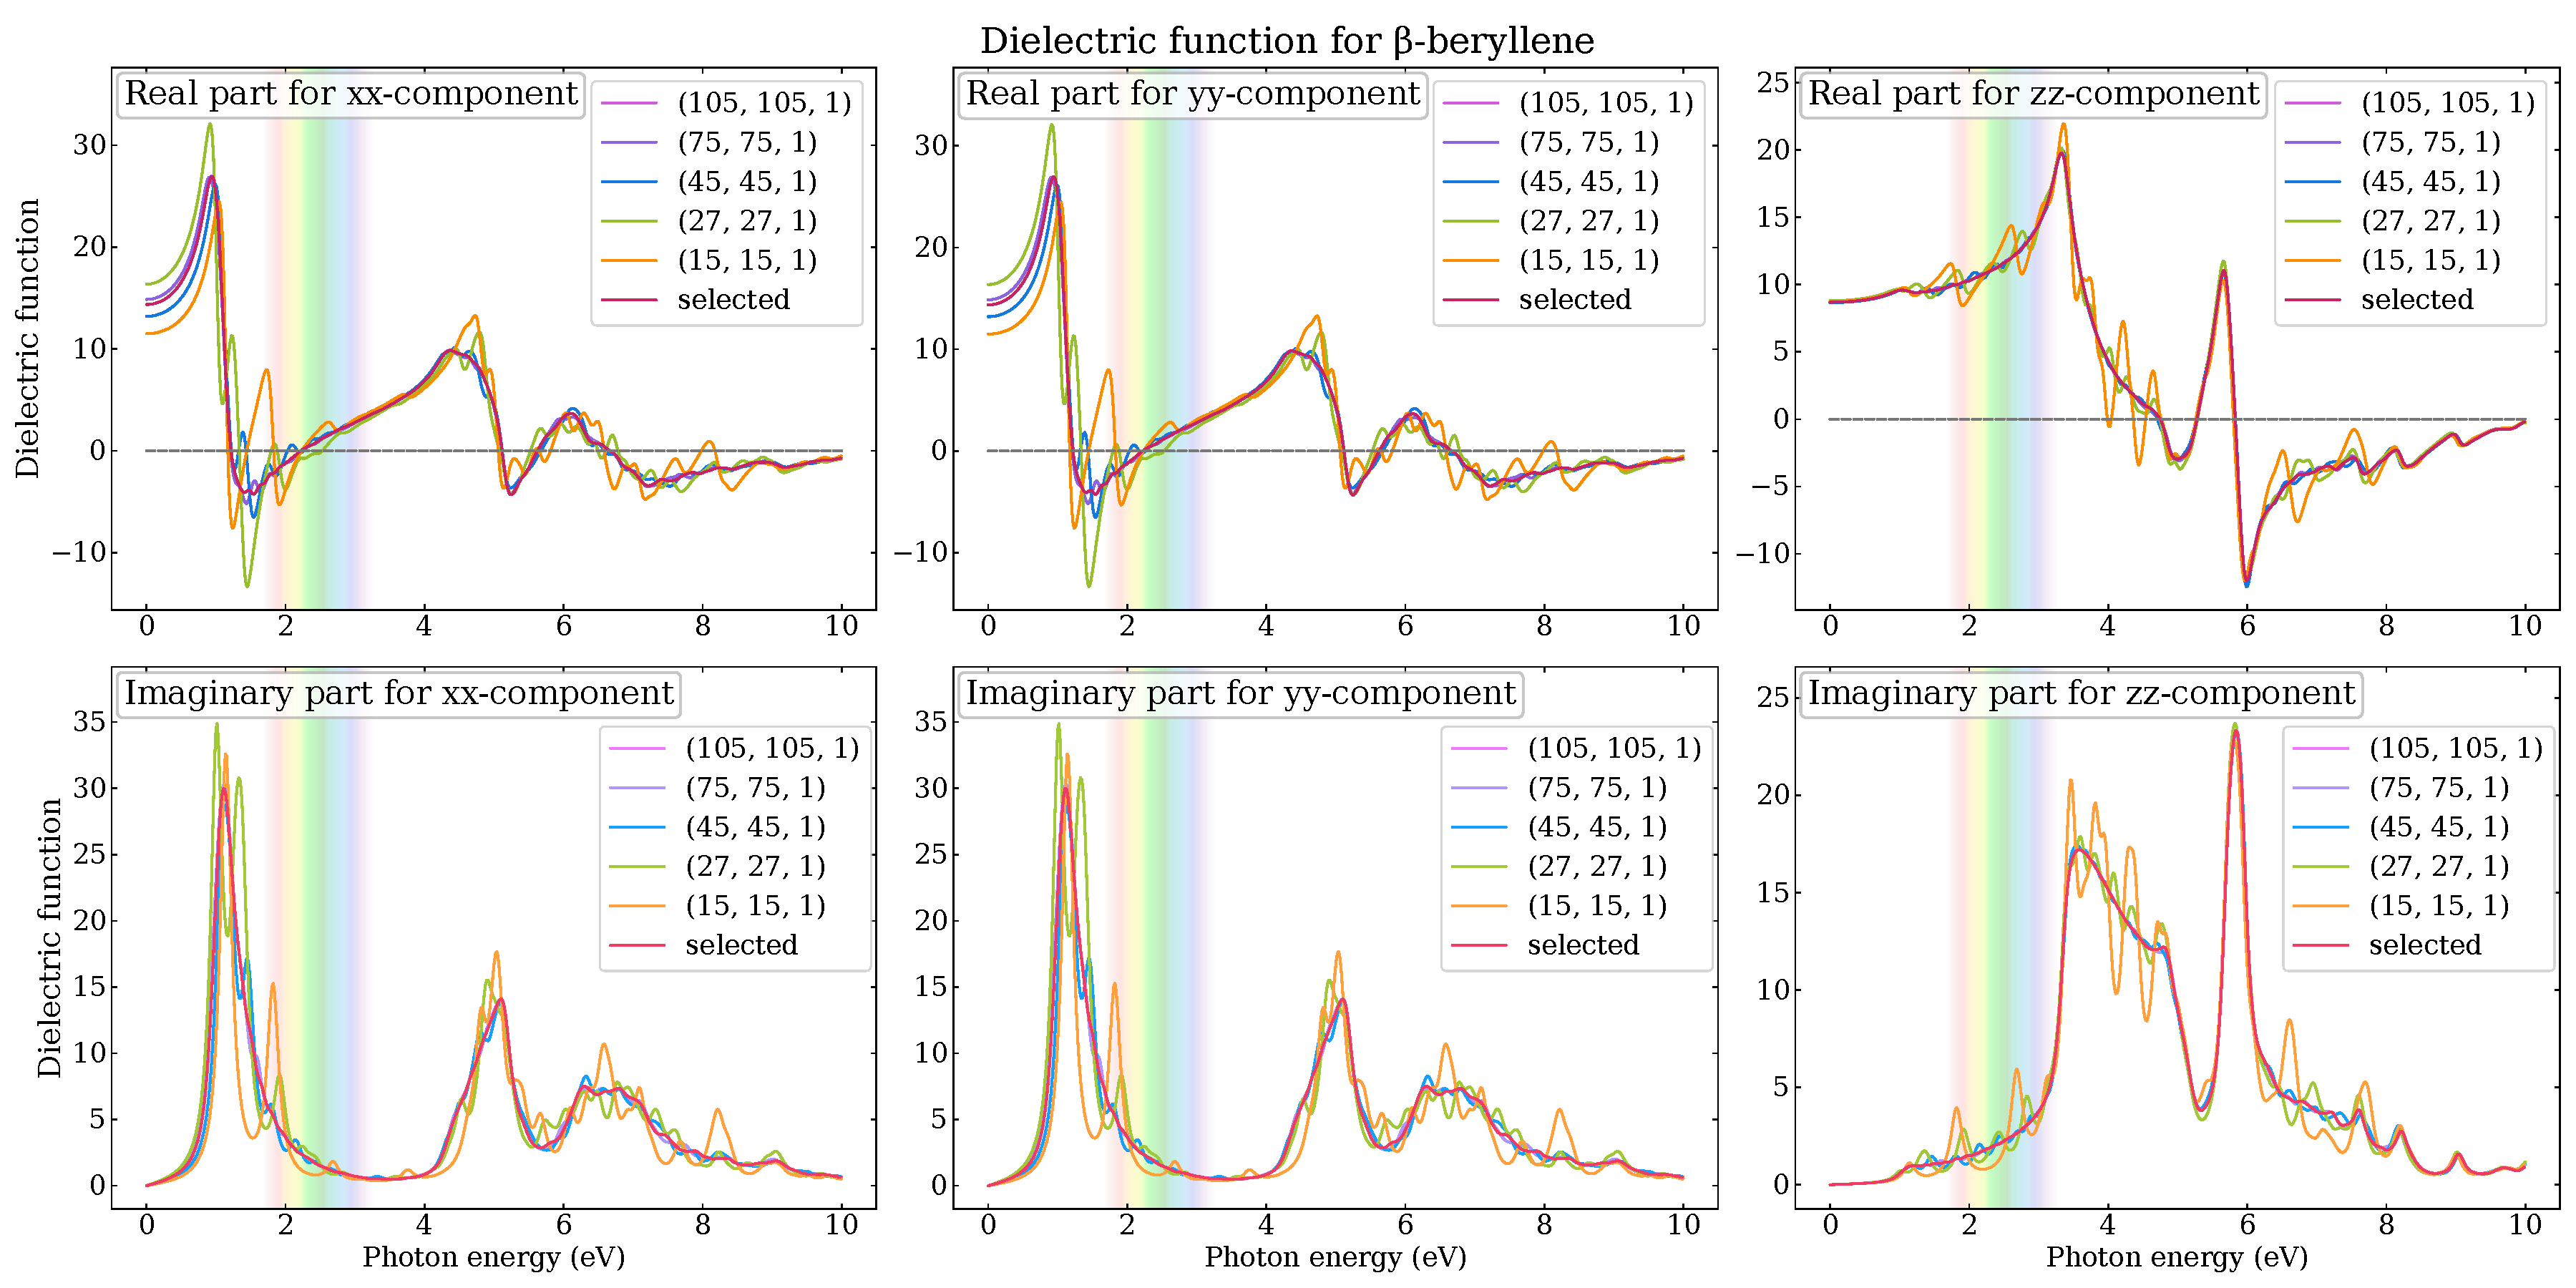
\includegraphics[width=1.0\linewidth]{figures_proj3/convergence_dielectric_kpoints_beta-beryllene_thesis.pdf}
\caption{Real and imaginary parts of the dielectric function for $\beta$-beryllene,
calculated with different k-point meshes.}
\label{fig:proj3_beta_dielectric_kpoint_convergence}
\end{figure}

\begin{figure}[!htbp]
\centering
    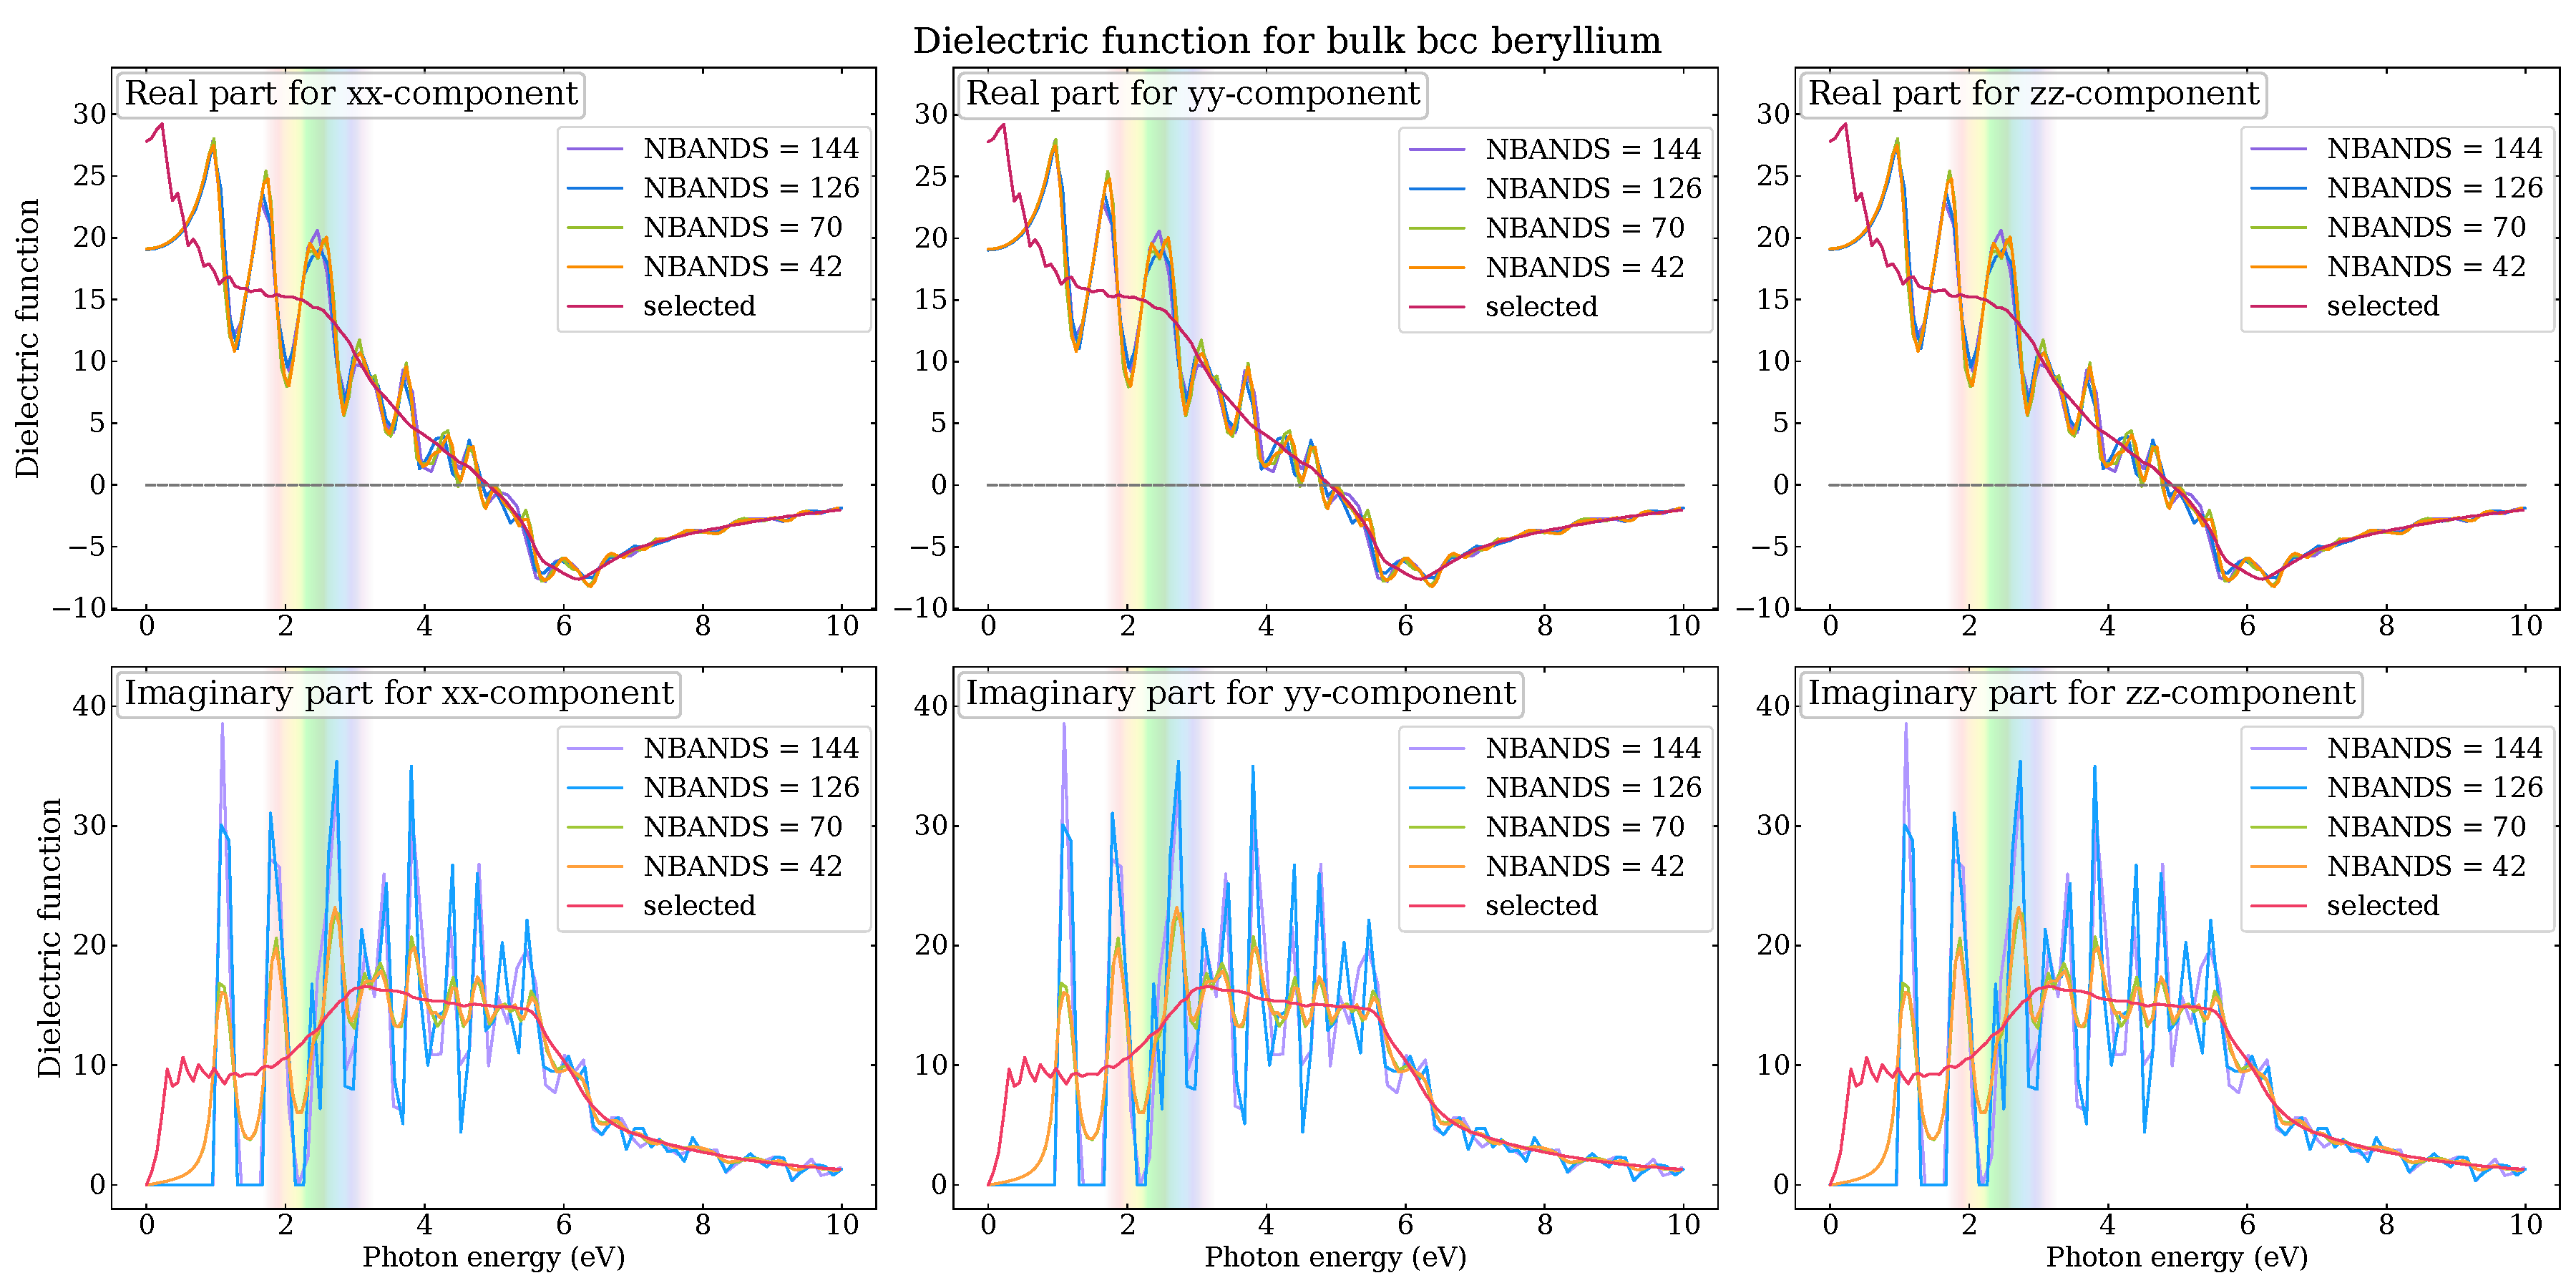
\includegraphics[width=1.0\linewidth]{figures_proj3/convergence_dielectric_nbands_bcc-beryllium_thesis.pdf}
\caption{Real and imaginary parts of the dielectric function for bulk bcc beryllium,
calculated with different total numbers of bands.}
\label{fig:proj3_bcc_dielectric_nbands_convergence}
\end{figure}

\begin{figure}[!htbp]
\centering
    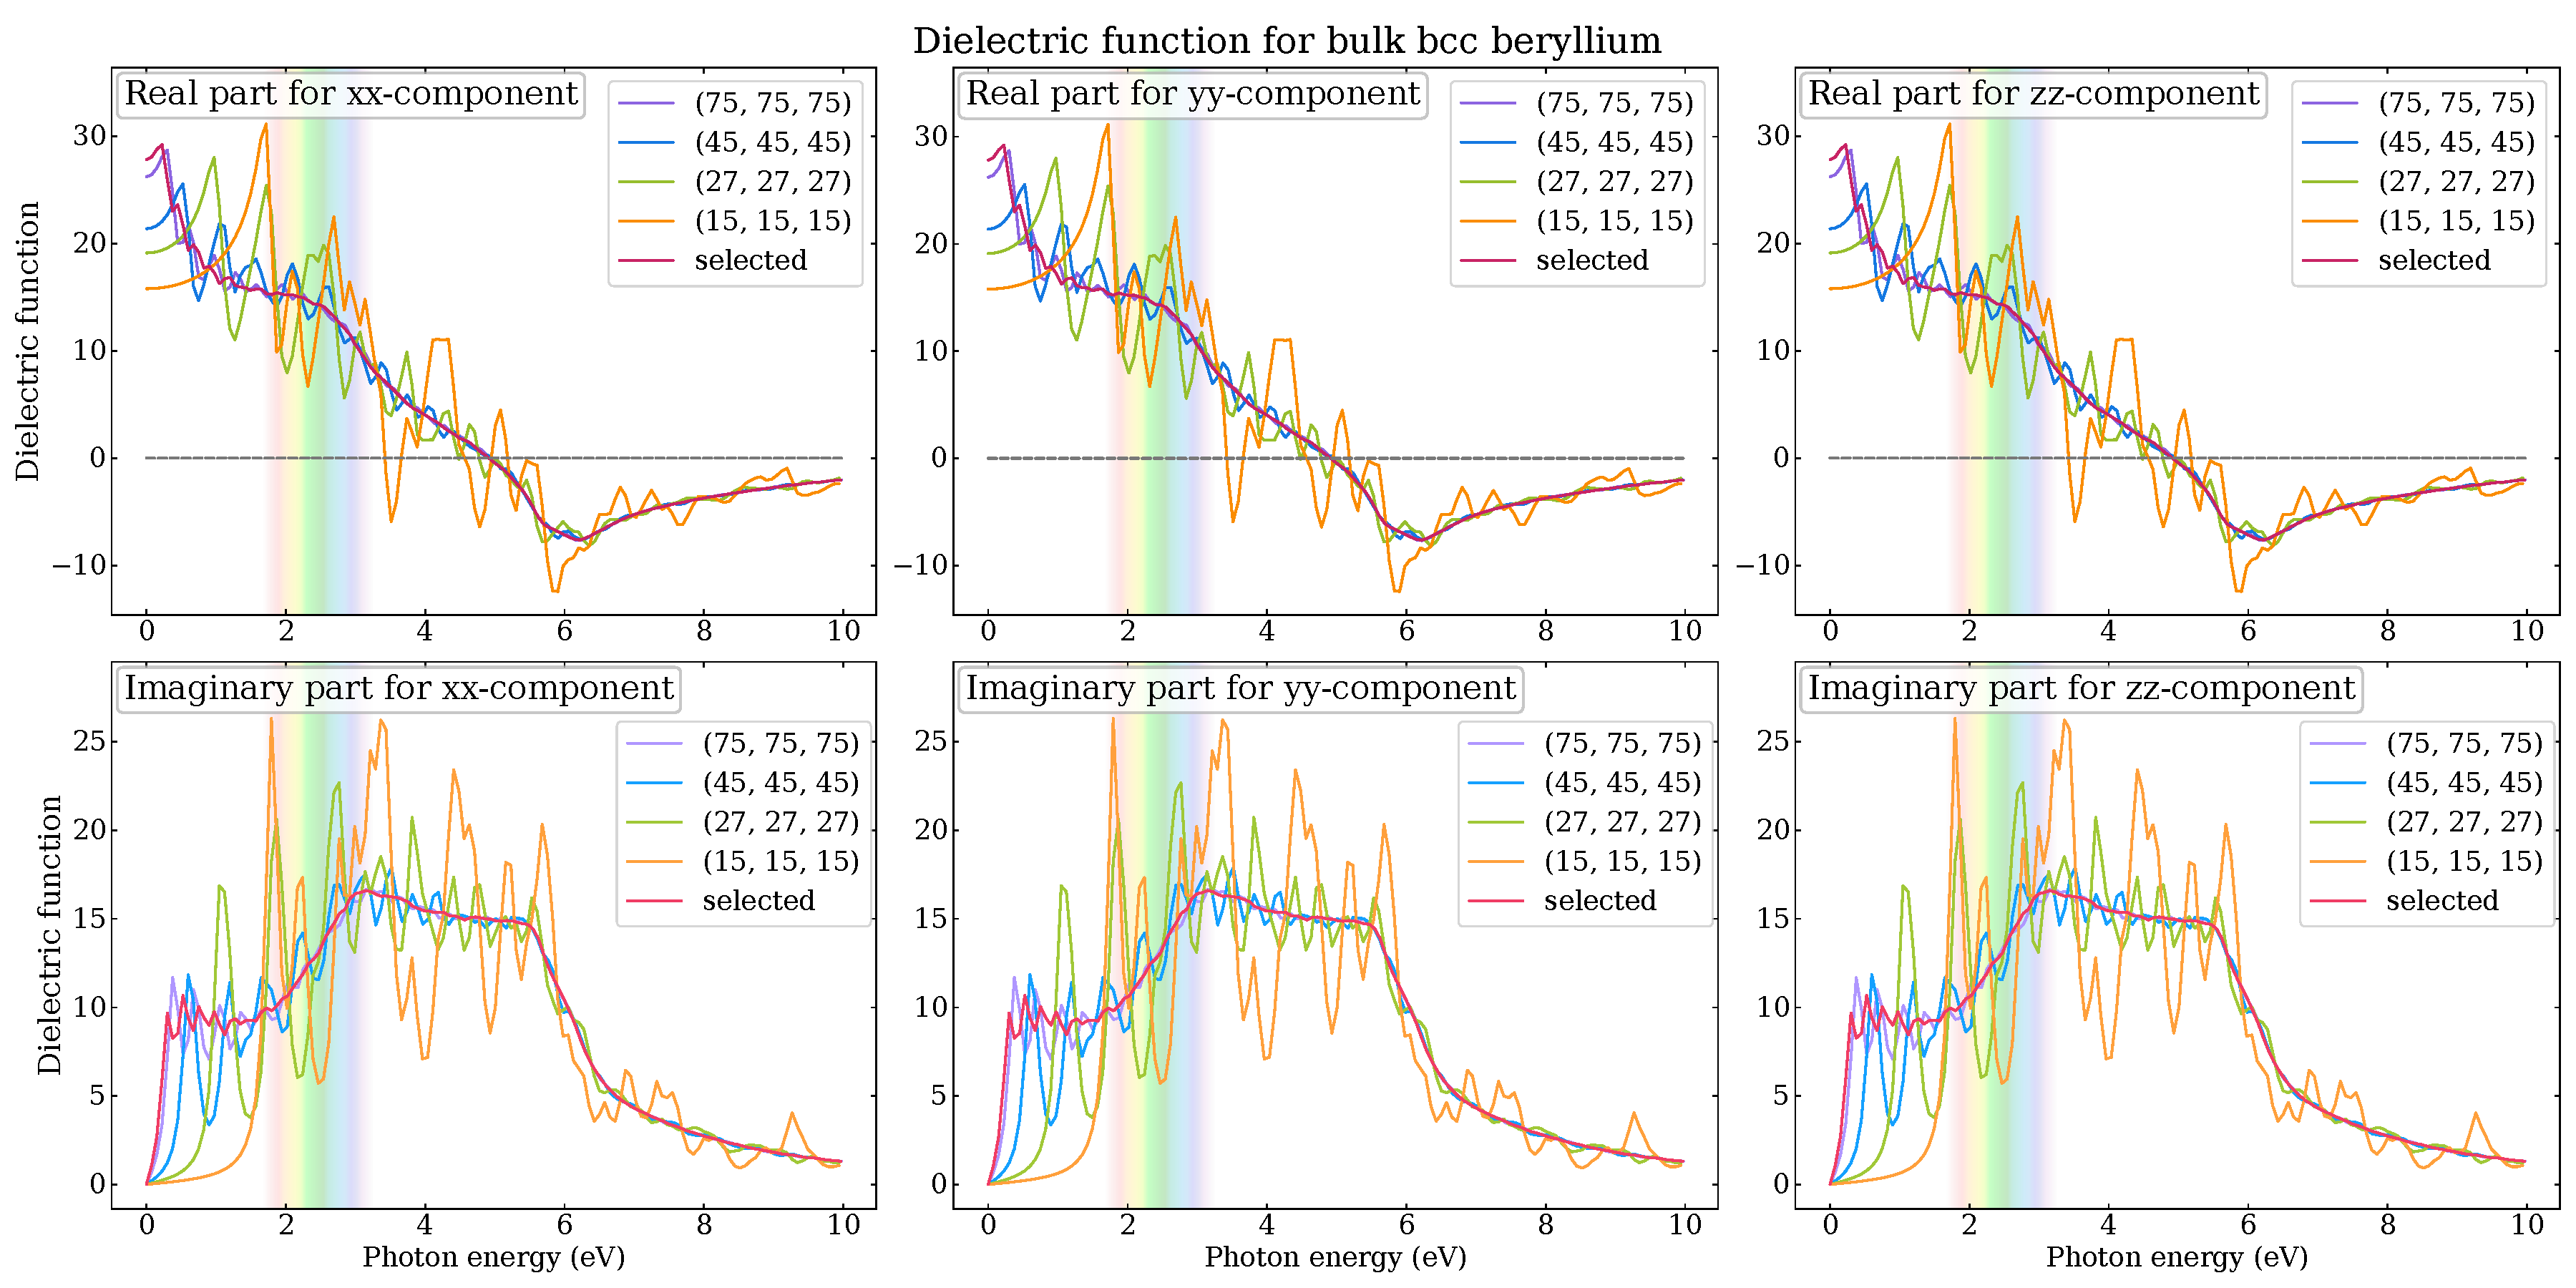
\includegraphics[width=1.0\linewidth]{figures_proj3/convergence_dielectric_kpoints_bcc-beryllium_thesis.pdf}
\caption{Real and imaginary parts of the dielectric function for bulk bcc beryllium,
calculated with different k-point meshes.}
\label{fig:proj3_bcc_dielectric_kpoint_convergence}
\end{figure}

\begin{figure}[!htbp]
\centering
    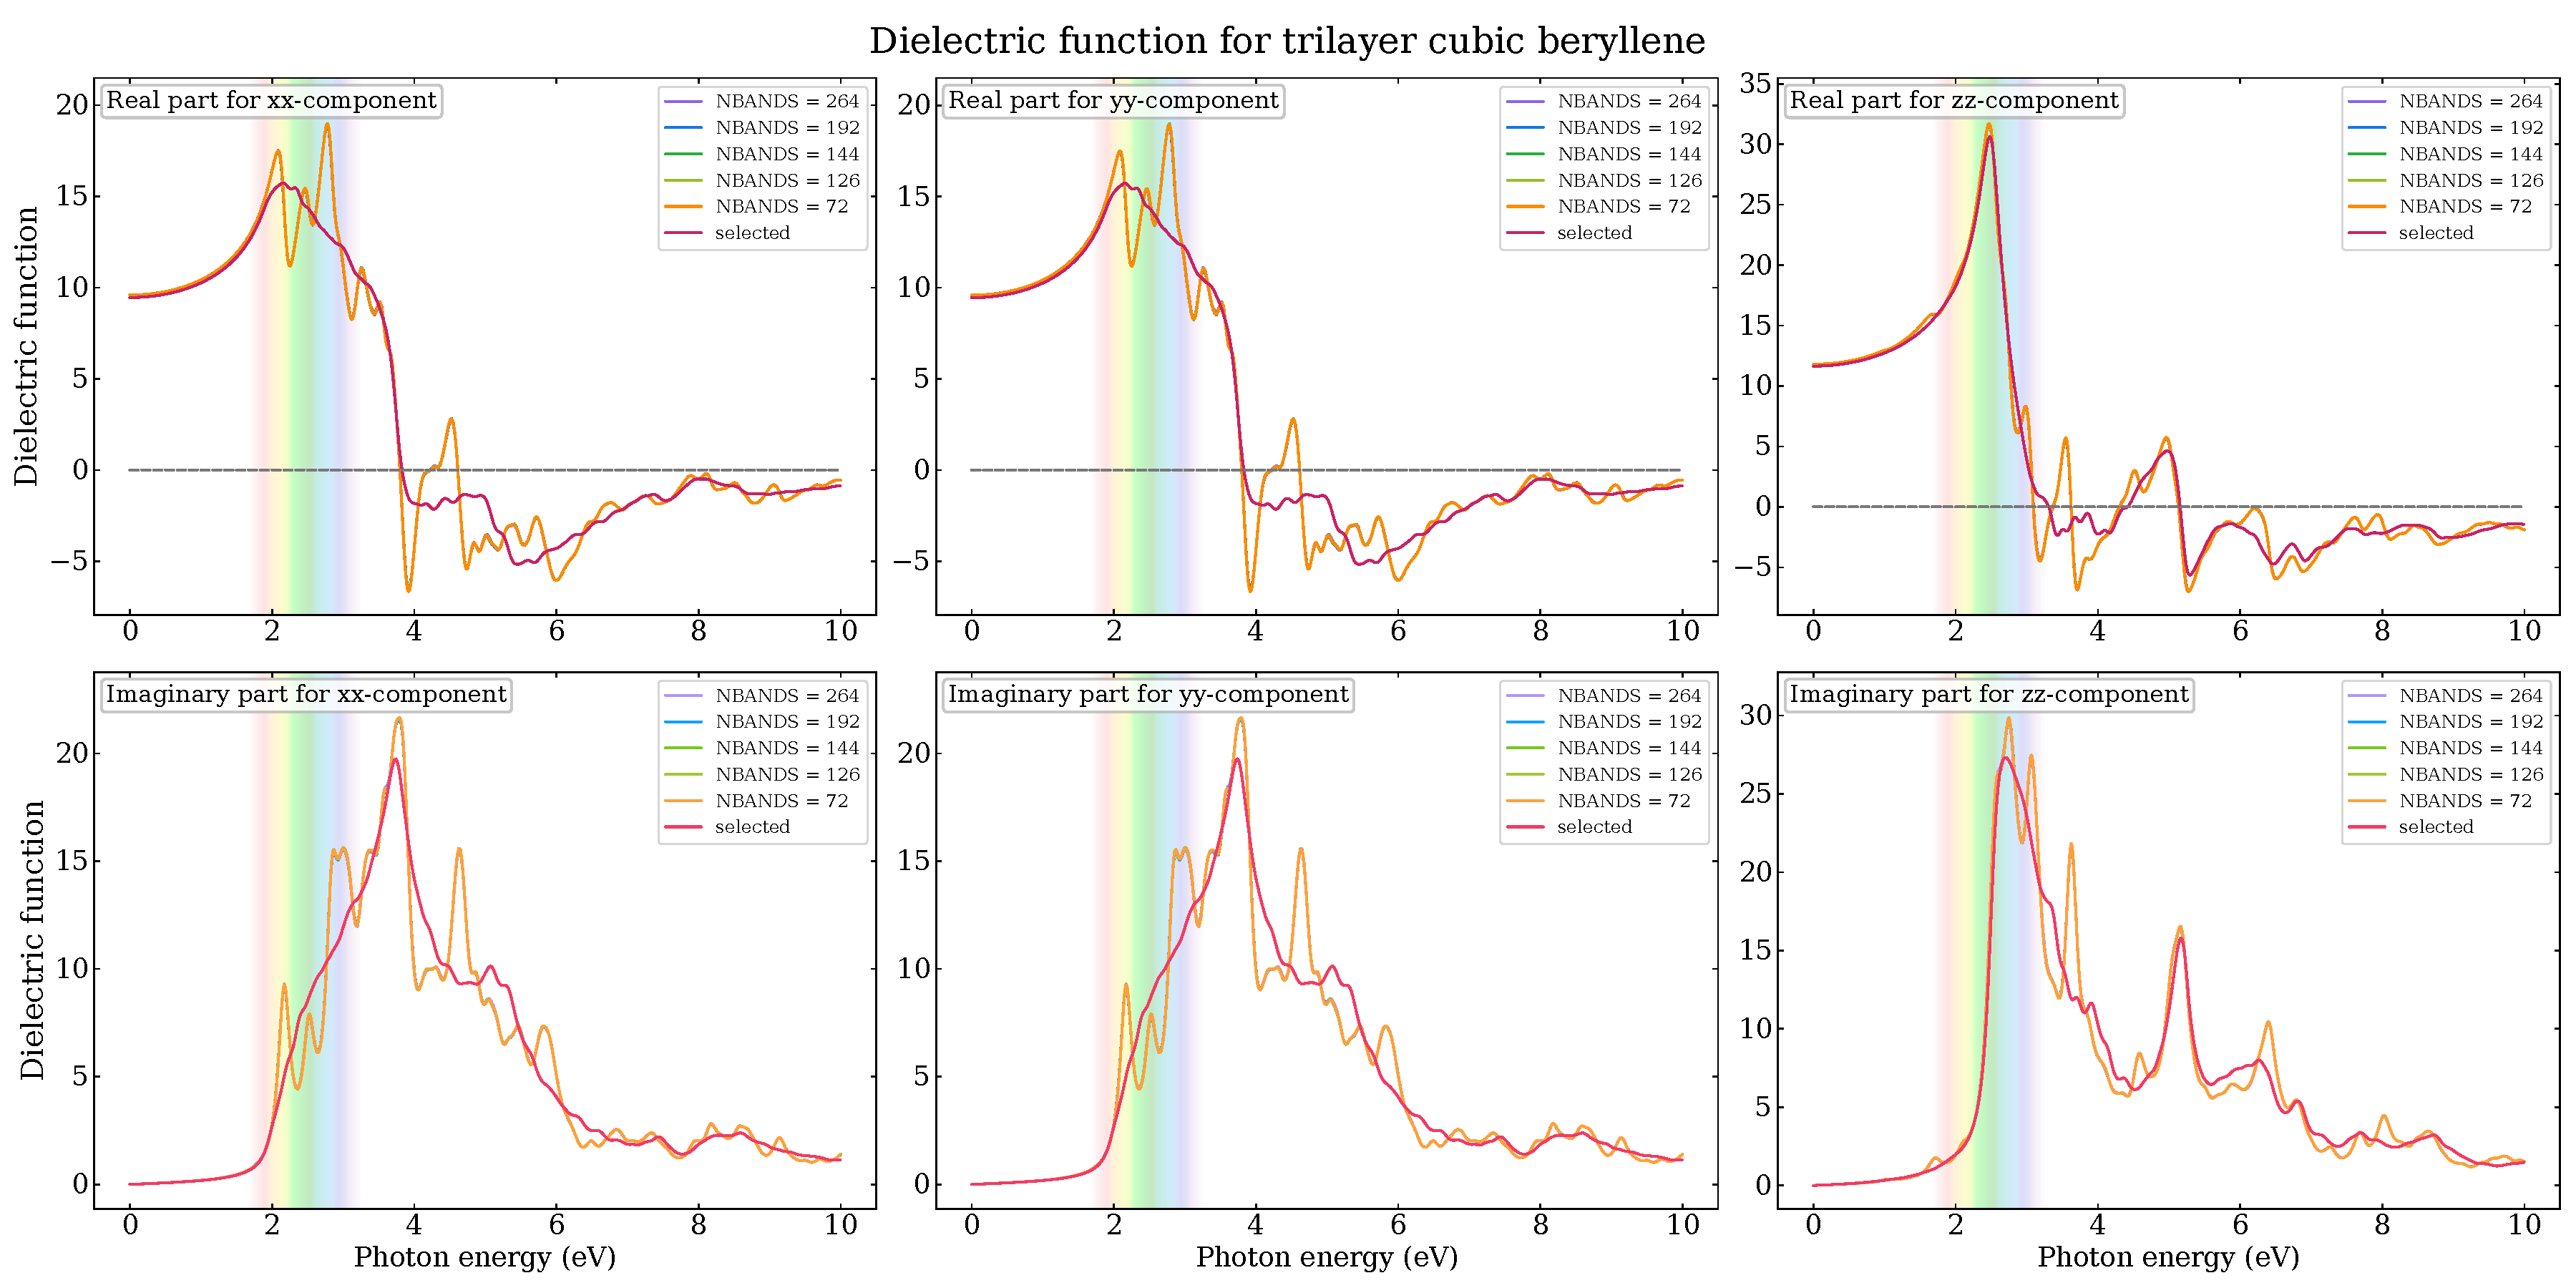
\includegraphics[width=1.0\linewidth]{figures_proj3/convergence_dielectric_nbands_cubic-beryllene-trilayer_thesis.pdf}
\caption{Real and imaginary parts of the dielectric function for trilayer cubic beryllene,
calculated with different total numbers of bands.}
\label{fig:proj3_cubic_dielectric_nbands_convergence}
\end{figure}

\begin{figure}[!htbp]
\centering
    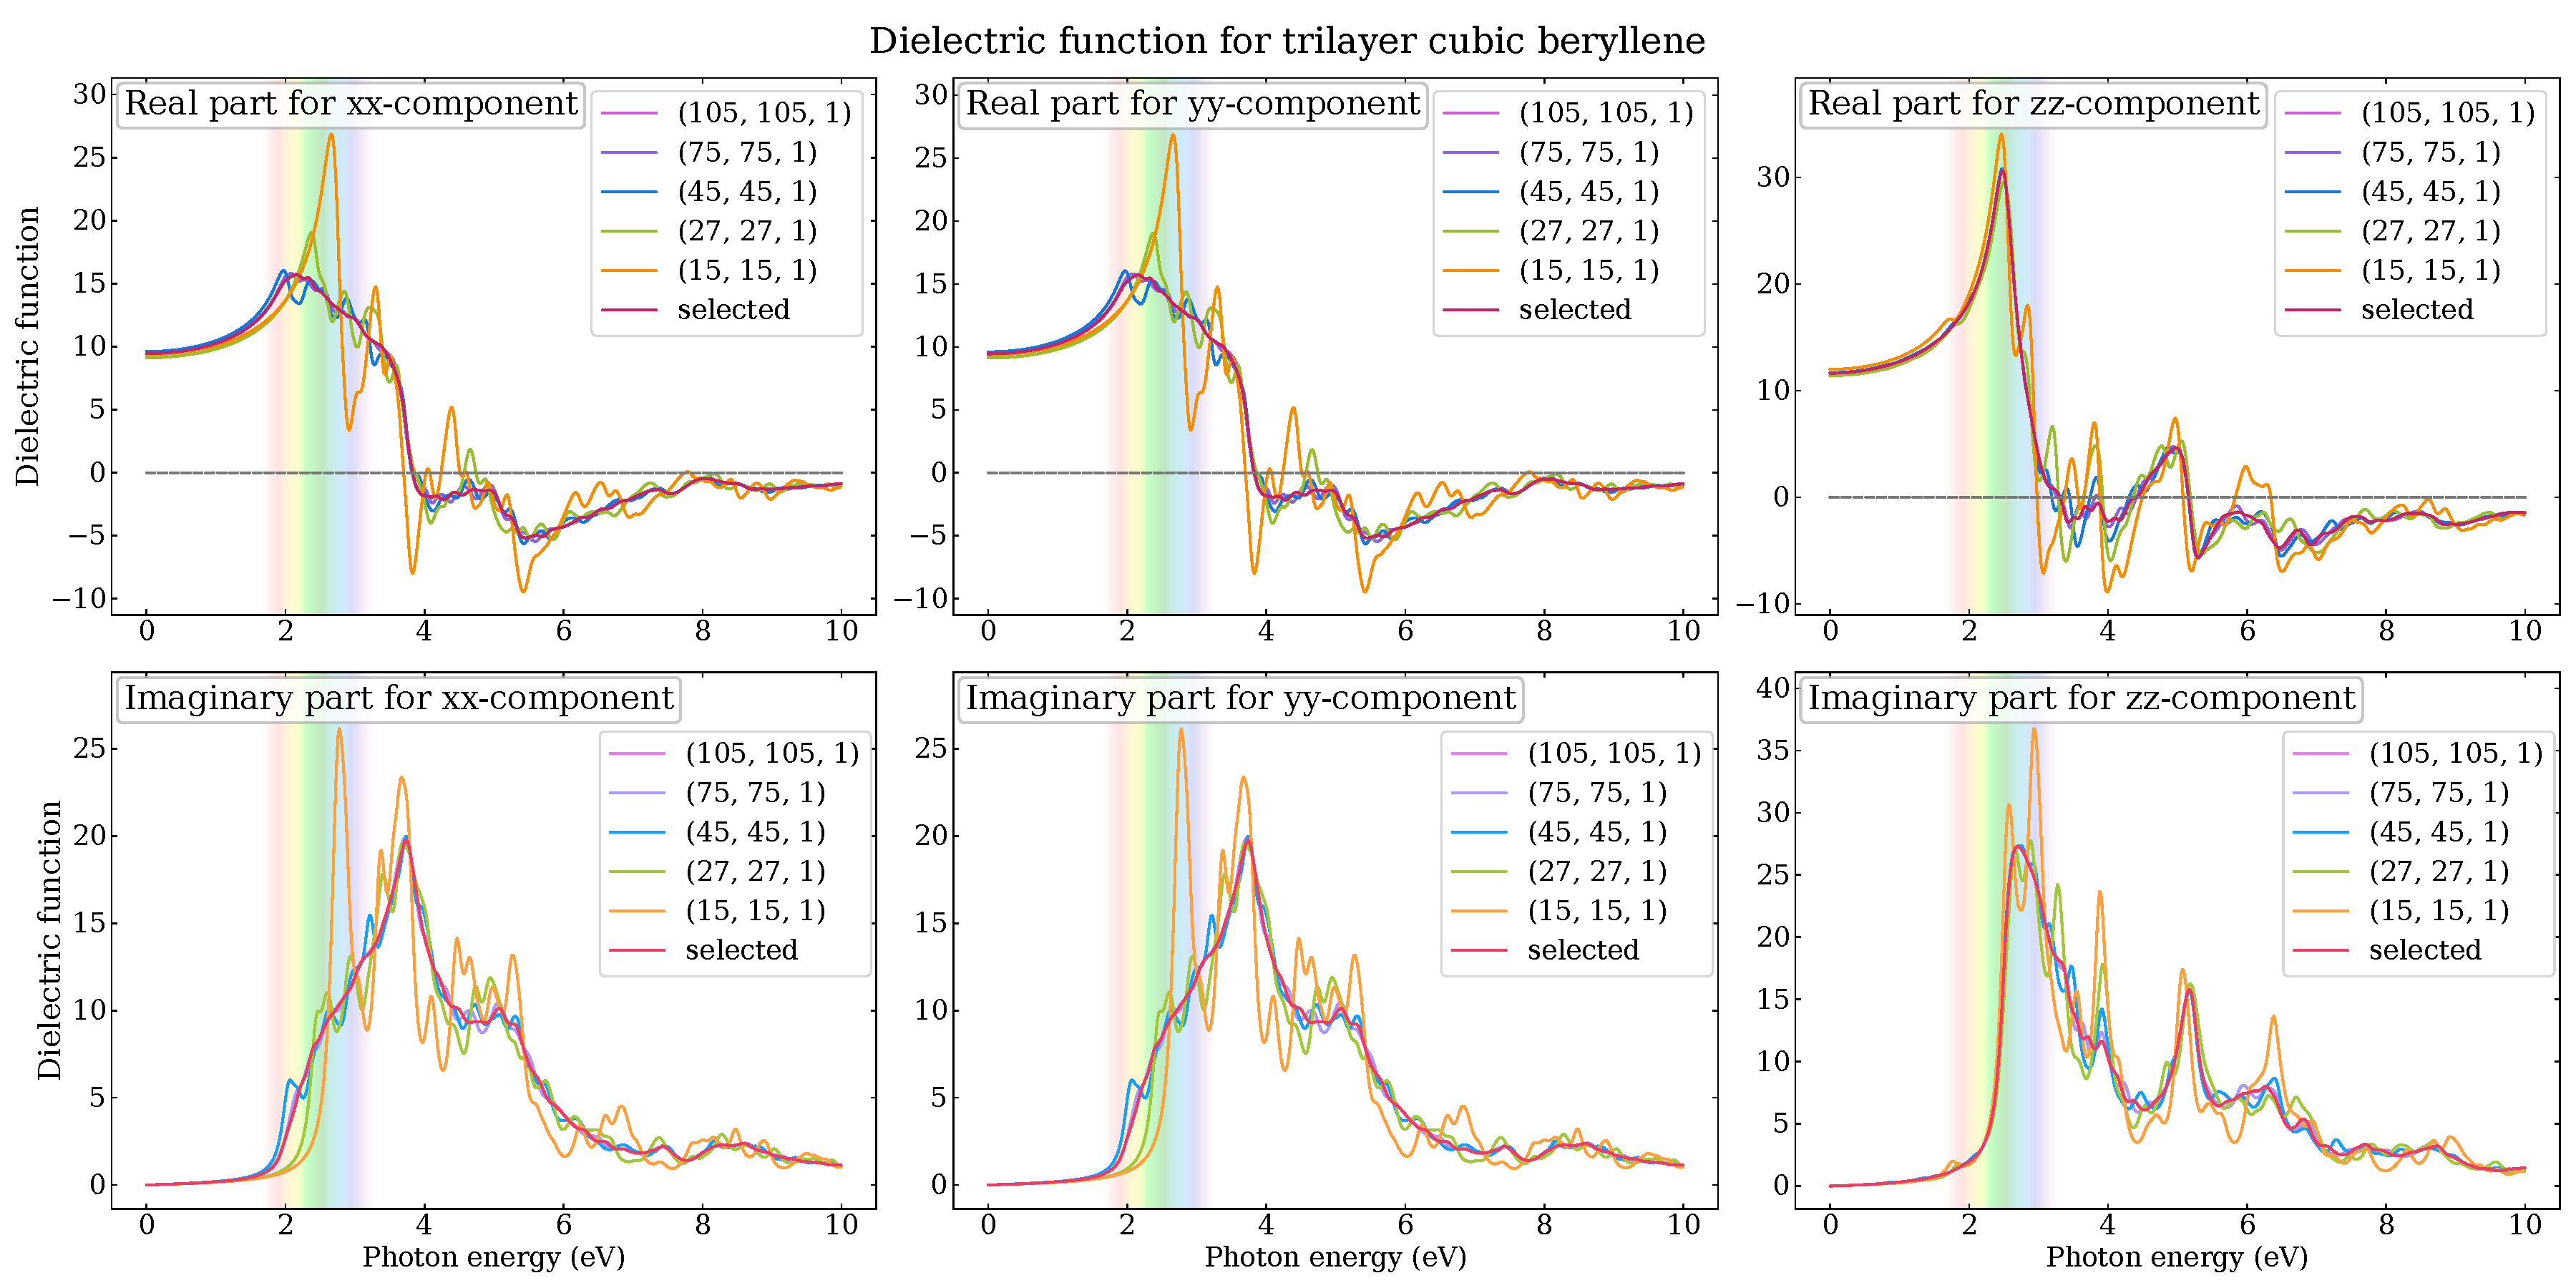
\includegraphics[width=1.0\linewidth]{figures_proj3/convergence_dielectric_kpoints_cubic-beryllene-trilayer_thesis.pdf}
\caption{Real and imaginary parts of the dielectric function for trilayer cubic beryllene,
calculated with different k-point meshes.}
\label{fig:proj3_cubic_dielectric_kpoint_convergence}
\end{figure}

\subsection*{Phonon dispersions, Brillouin zones, and band structures}

The calculated phonon-dispersion curves and band structures for $\alpha$-beryllene,
$\beta$-beryllene, bulk hcp beryllium, and bulk bcc beryllium
are shown in figures~\ref{fig:proj3_phonon_dispersion} and~\ref{fig:proj3_band_structures}.
The phonon dispersions are calculated with PBE without a dispersion correction.
Bulk bcc beryllium has an imaginary frequency of $3.90\mathrm{i}$~\si{\tera\hertz} at the $\mathrm{N}$ point,
which is commensurate with the $4 \times 4 \times 4$ supercell.
This instability is expected for the high-temperature bcc phase of beryllium,
which is stabilized by anharmonicity.
The Brillouin zones used for the hexagonal and distorted hexagonal cells are shown in figure~\ref{fig:proj3_brillouin_zones}.
For 1H-$\beta$-beryllene and 2H-$\beta$-beryllene,
the band structures and phonon dispersions use the path $\Gamma$--$\mathrm{X}$--$\mathrm{K}$--$\Gamma$--$\mathrm{Y}$--$\mathrm{K}'$--$\mathrm{M}$--$\Gamma$ shown in figure~\ref{fig:proj3_brillouin_zones}(b).
These cells are continuous distortions of the hexagonal cell,
with angles of \qty{117}{\degree} and \qty{133}{\degree} between the lattice vectors.
Therefore, $\mathrm{K}$ and $\mathrm{K}'$ derive from the zone corners of the hexagonal cell,
and $\mathrm{X}$, $\mathrm{Y}$, and $\mathrm{M}$ from its three equivalent $\mathrm{M}$ points.
With the $P1$ and $P\bar{1}$ symmetry of 1H-$\beta$-beryllene and 2H-$\beta$-beryllene,
together with time-reversal symmetry,
this path covers the irreducible part of the zone boundary.
Within a tolerance of \qty{1e-3}{\angstrom},
the two cells have $Cm$ and $C2/m$ symmetry.
This higher symmetry makes the $\Gamma$--$\mathrm{Y}$ and $\Gamma$--$\mathrm{M}$ lines of 1H-$\beta$-beryllene and the $\Gamma$--$\mathrm{X}$ and $\Gamma$--$\mathrm{Y}$ lines of 2H-$\beta$-beryllene equivalent.
The calculated PBE bands along these lines differ by at most \qty{3.3}{\milli\electronvolt} and \qty{7.3}{\milli\electronvolt},
respectively.

\begin{figure}[!htbp]
\centering
\begin{tabular}{@{}cc@{}}
% \begin{tabular}{cc}
    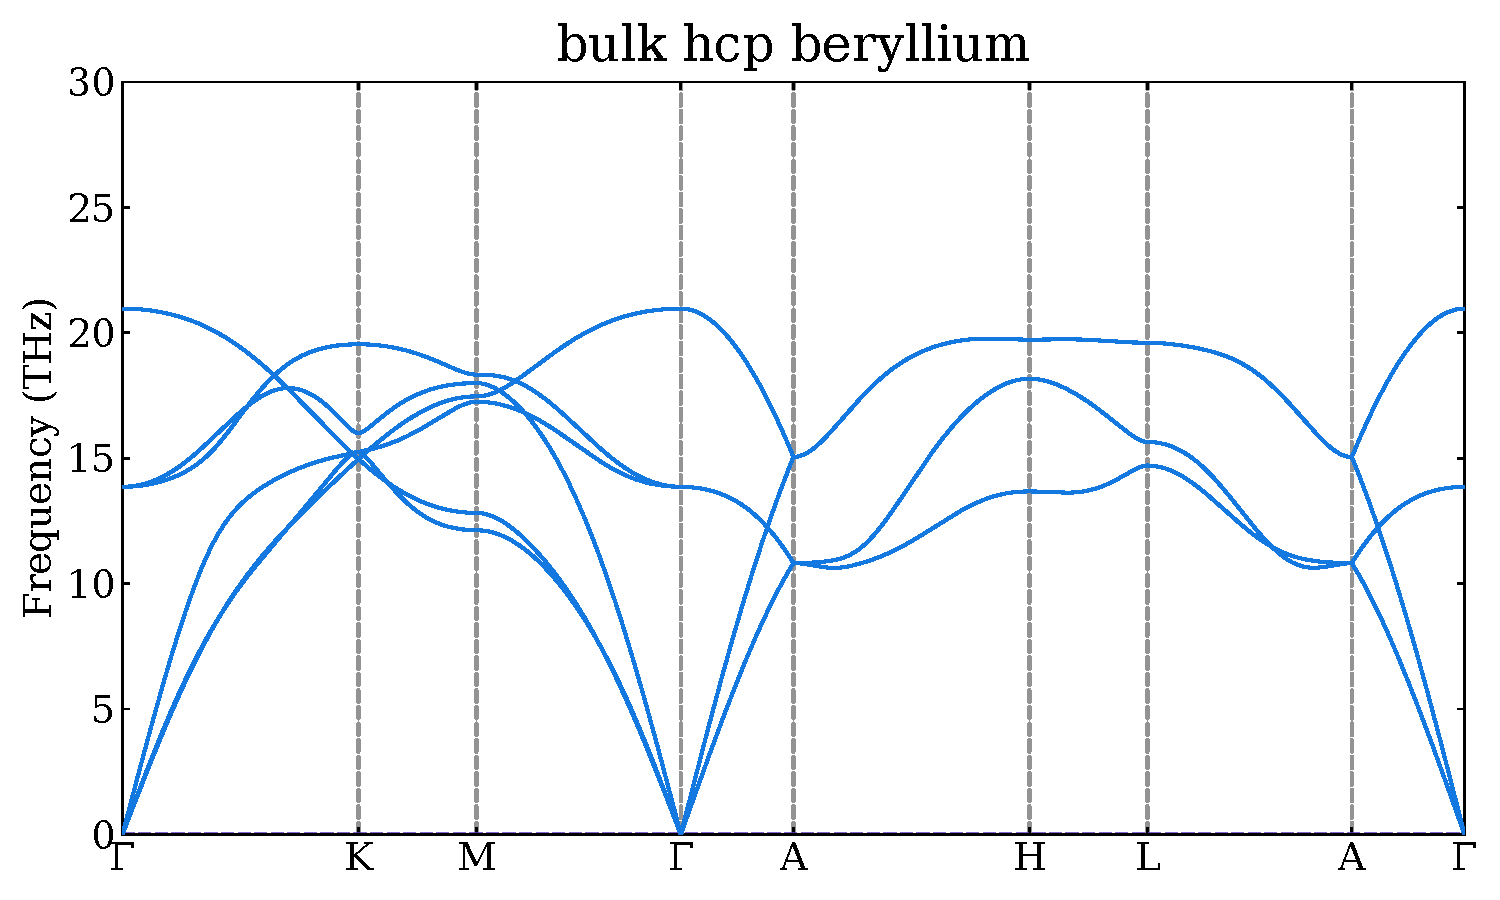
\includegraphics[width=0.40\linewidth]{figures_proj3/phonon_hcp-beryllium_thesis.pdf}&
    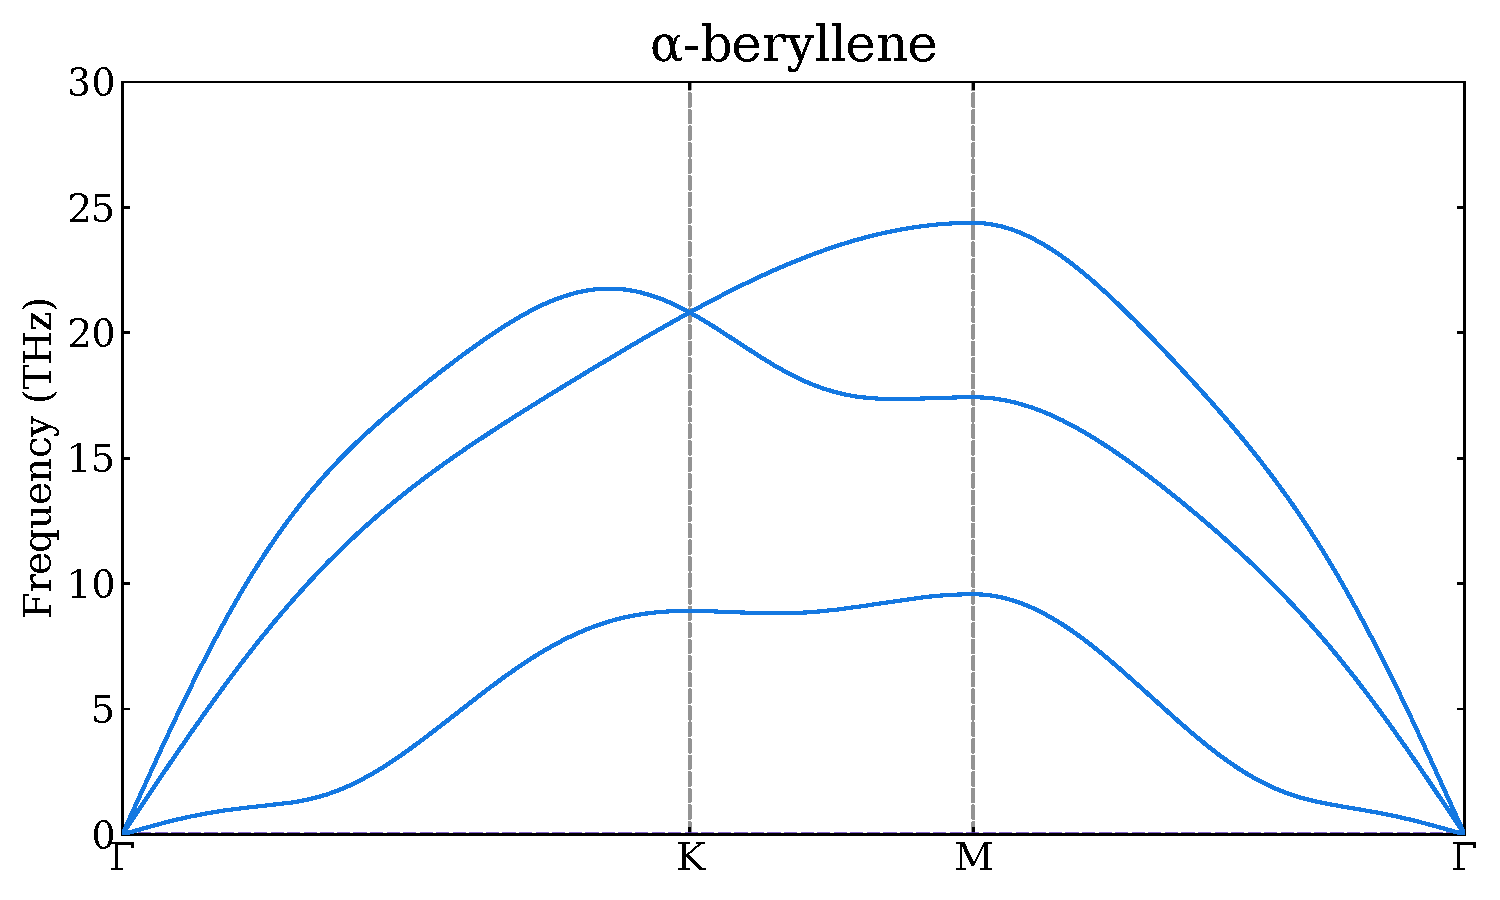
\includegraphics[width=0.40\linewidth]{figures_proj3/phonon_alpha-beryllene_thesis.pdf}\\
    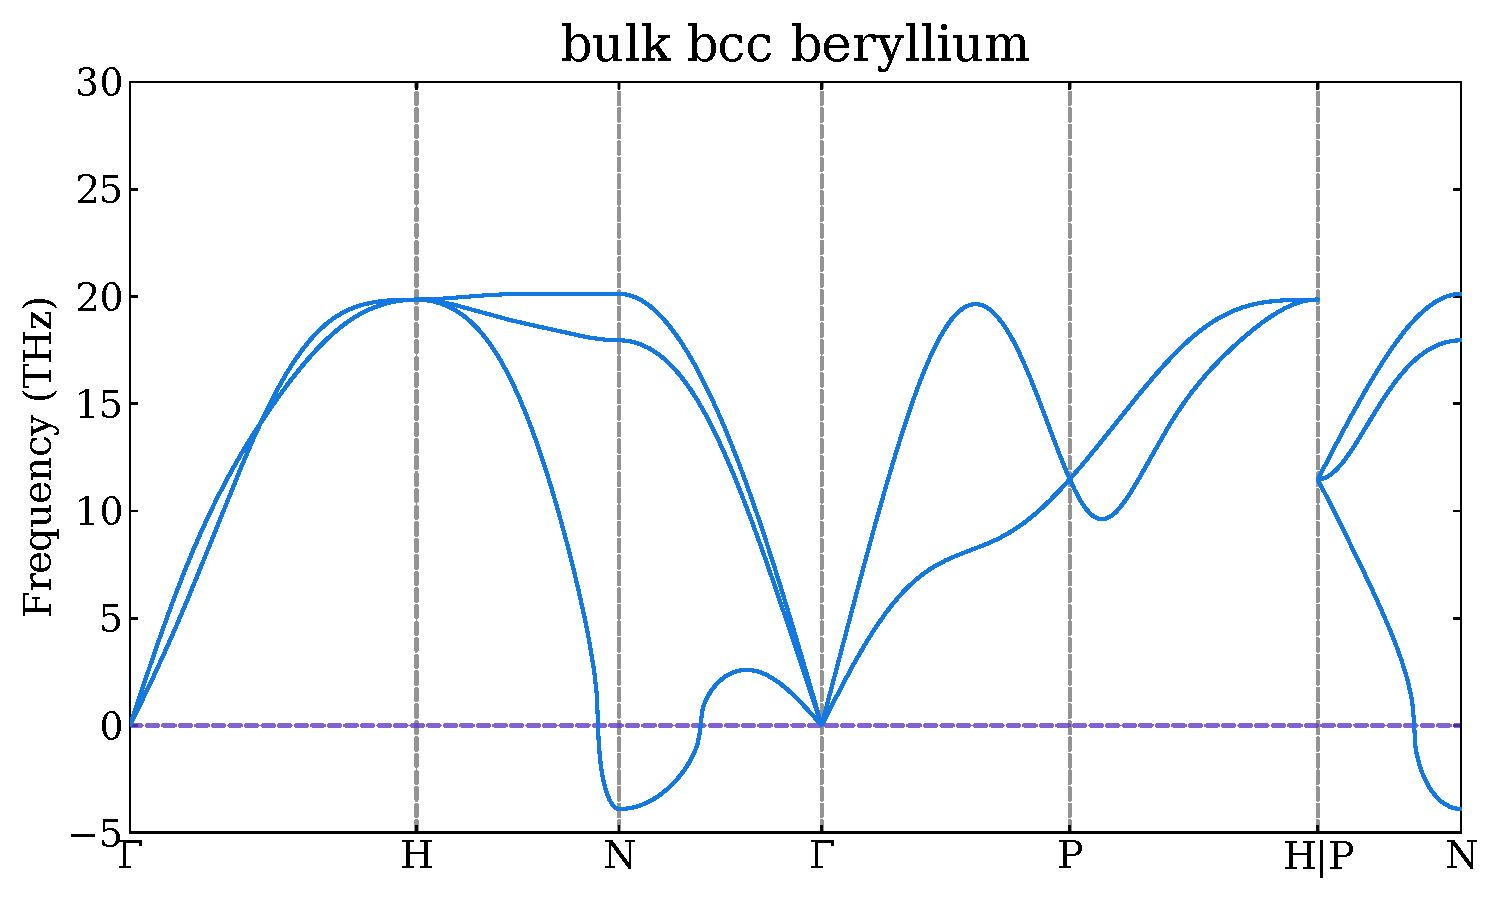
\includegraphics[width=0.40\linewidth]{figures_proj3/phonon_bcc-beryllium_thesis.pdf}&
    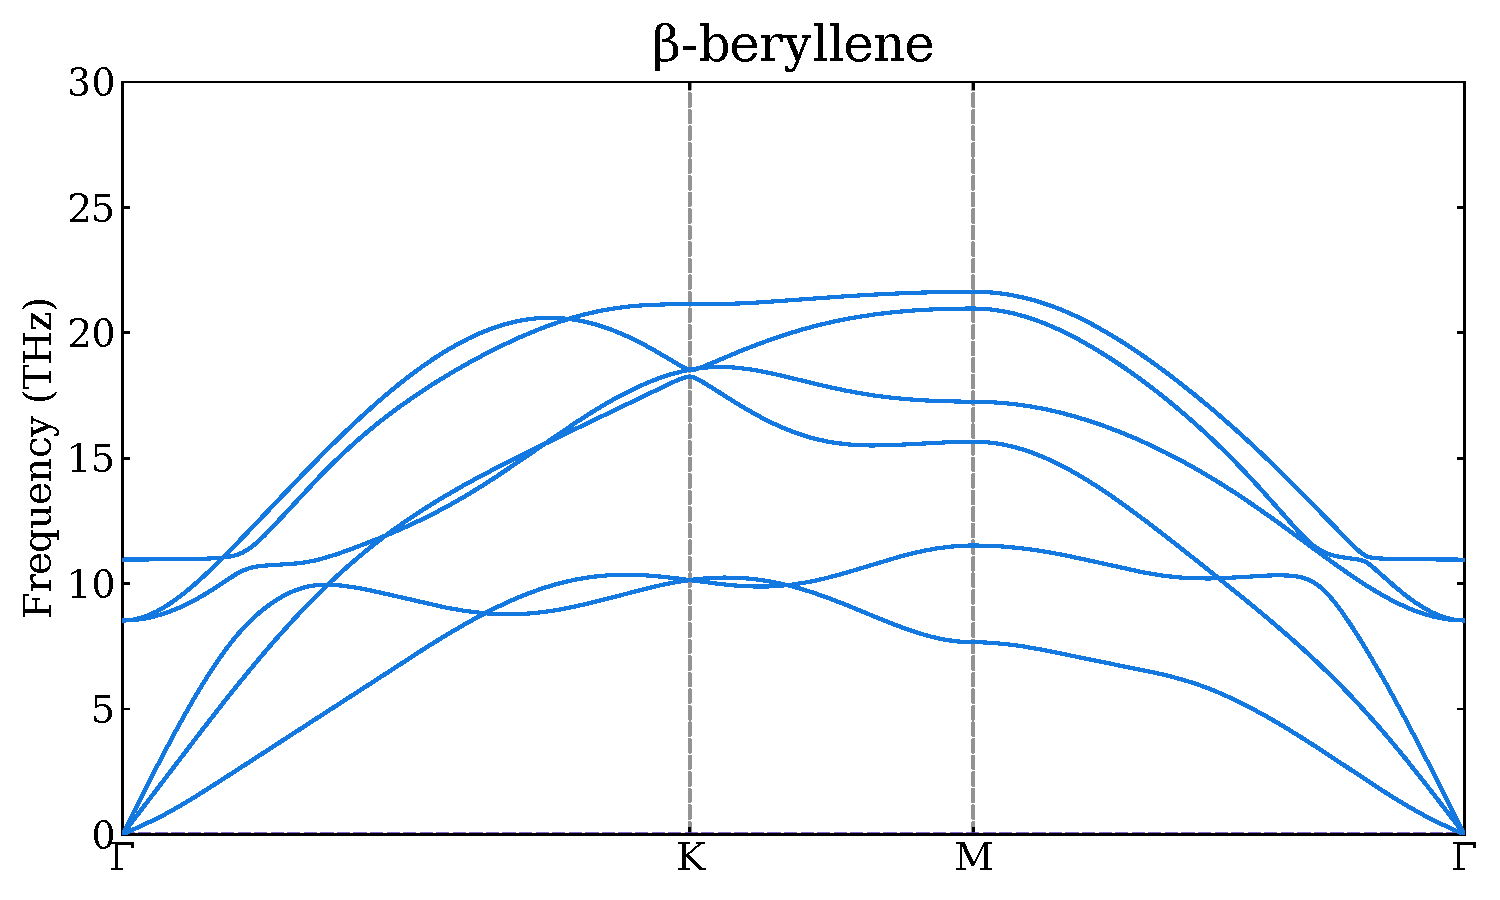
\includegraphics[width=0.40\linewidth]{figures_proj3/phonon_beta-beryllene_thesis.pdf}
\end{tabular}
\caption{Phonon-dispersion curves for bulk hcp beryllium, $\alpha$-beryllene, bulk bcc beryllium, and $\beta$-beryllene.
Imaginary frequencies are shown as negative values.}
\label{fig:proj3_phonon_dispersion}
\end{figure}

\begin{figure}[!htbp]
\centering
    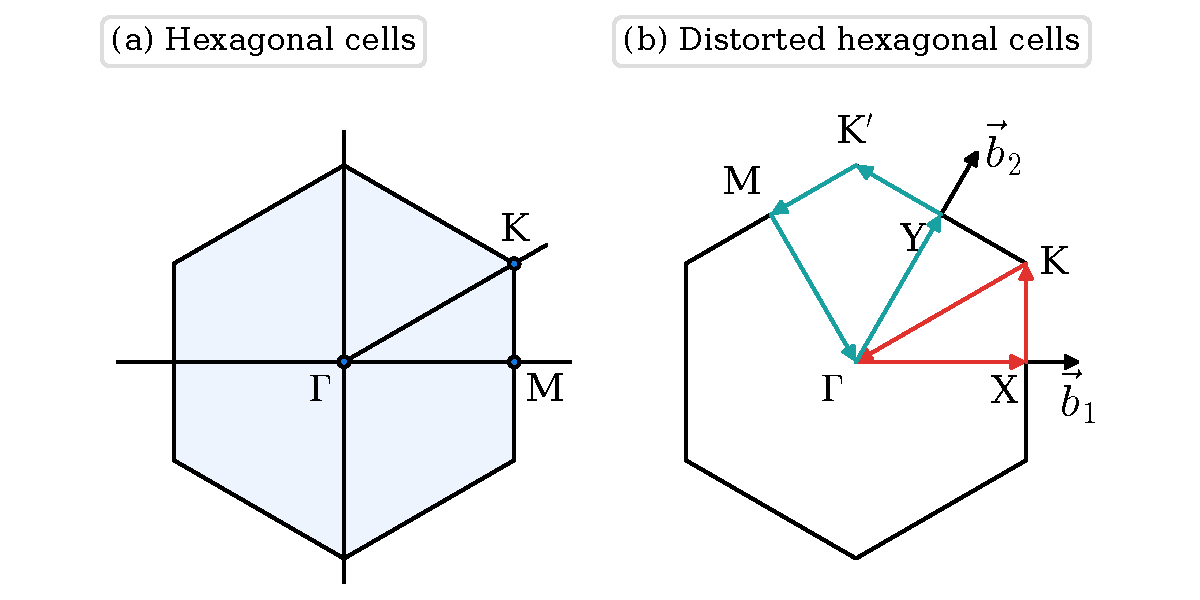
\includegraphics[width=0.80\linewidth]{figures_proj3/brillouin_zone_thesis.pdf}
\caption{Schematic Brillouin zones of the hexagonal and distorted hexagonal cells.
(a) Brillouin zone for the hexagonal unit cells of $\alpha$-beryllene, $\beta$-beryllene, and 2H-$\alpha$-beryllene.
(b) Brillouin zone for the distorted hexagonal cells of 1H-$\beta$-beryllene and 2H-$\beta$-beryllene,
with the path $\Gamma$--$\mathrm{X}$--$\mathrm{K}$--$\Gamma$--$\mathrm{Y}$--$\mathrm{K}'$--$\mathrm{M}$--$\Gamma$ used for their band structures and phonon dispersions.
$\vec{b}_{1}$ and $\vec{b}_{2}$ are the reciprocal lattice vectors of each relaxed cell,
and all coordinates are given in this basis.
$\mathrm{X}=\vec{b}_{1}/2$,
$\mathrm{Y}=\vec{b}_{2}/2$,
and $\mathrm{M}=(\vec{b}_{2}-\vec{b}_{1}\,)/2$,
which is equivalent to $(\vec{b}_{1}+\vec{b}_{2}\,)/2$,
are the time-reversal invariant momenta on the zone boundary.
$\mathrm{K}$ and $\mathrm{K}'=-\mathrm{K}+\vec{b}_{2}$ are the zone corners,
which are related by time reversal,
with $\mathrm{K}=(0.315,\,0.370)$ for 1H-$\beta$-beryllene and $(0.298,\,0.298)$ for 2H-$\beta$-beryllene.}
\label{fig:proj3_brillouin_zones}
\end{figure}

\begin{figure}[!htbp]
\centering
\begin{tabular}{@{}cc@{}}
% \begin{tabular}{cc}
    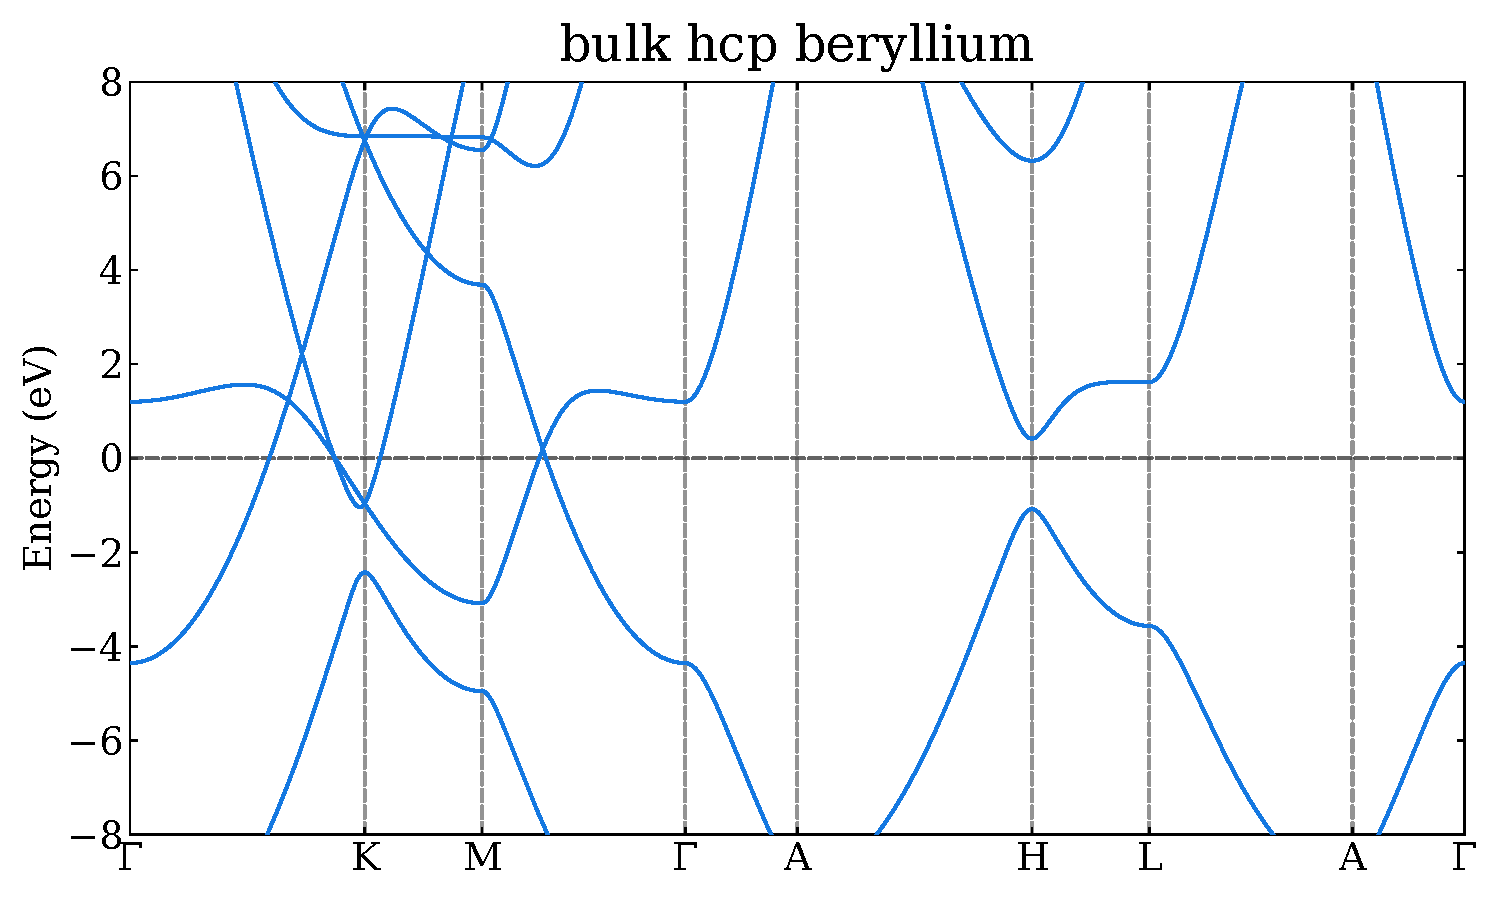
\includegraphics[width=0.40\linewidth]{figures_proj3/bands_hcp-beryllium_thesis.pdf}&
    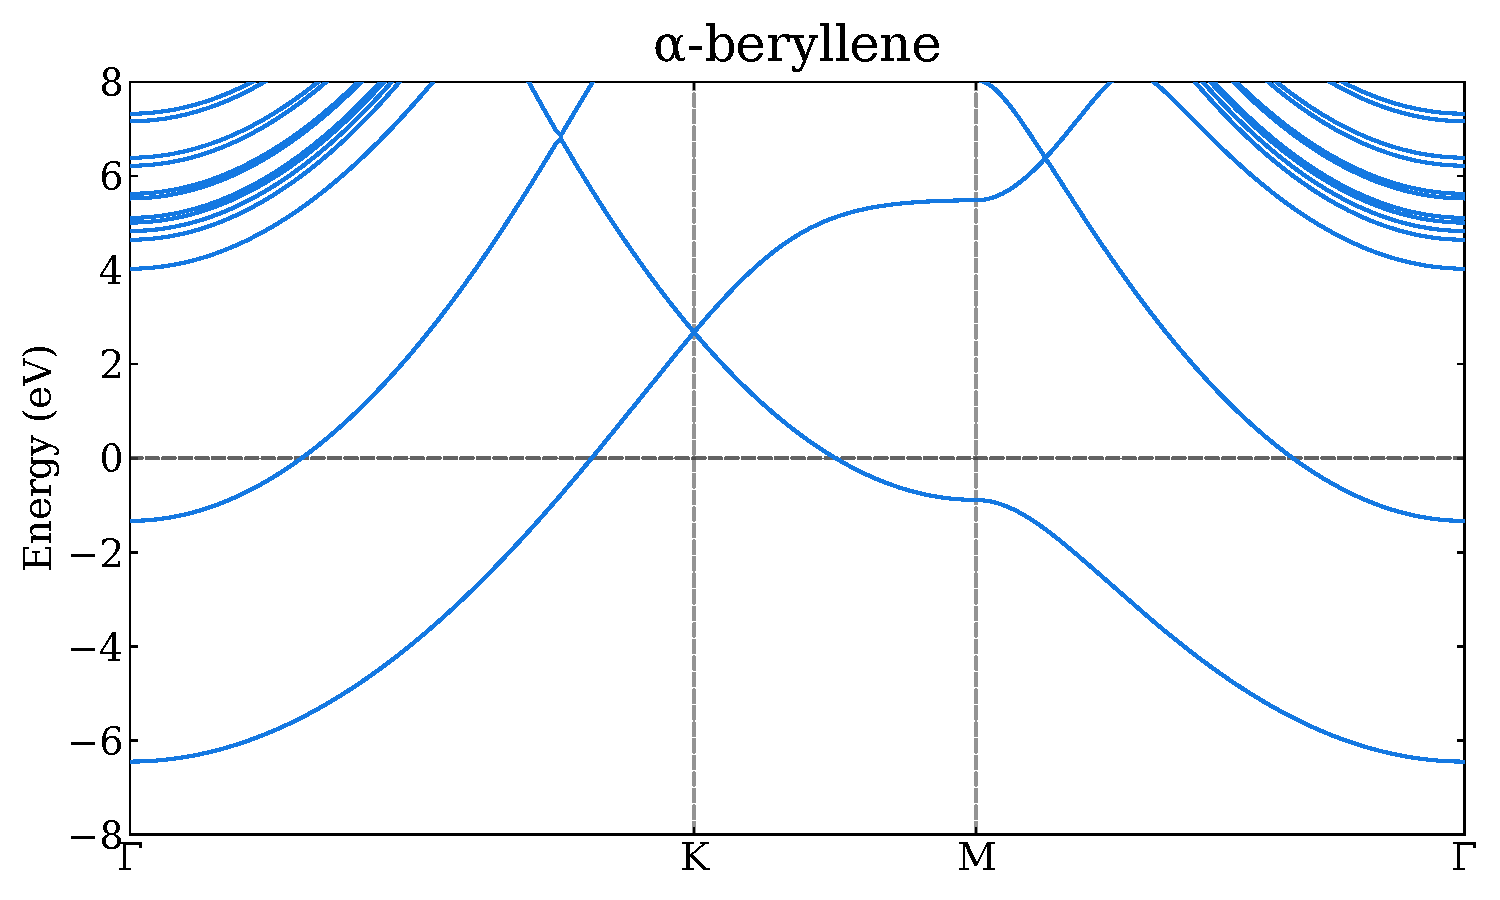
\includegraphics[width=0.40\linewidth]{figures_proj3/bands_alpha-beryllene_thesis.pdf}\\
    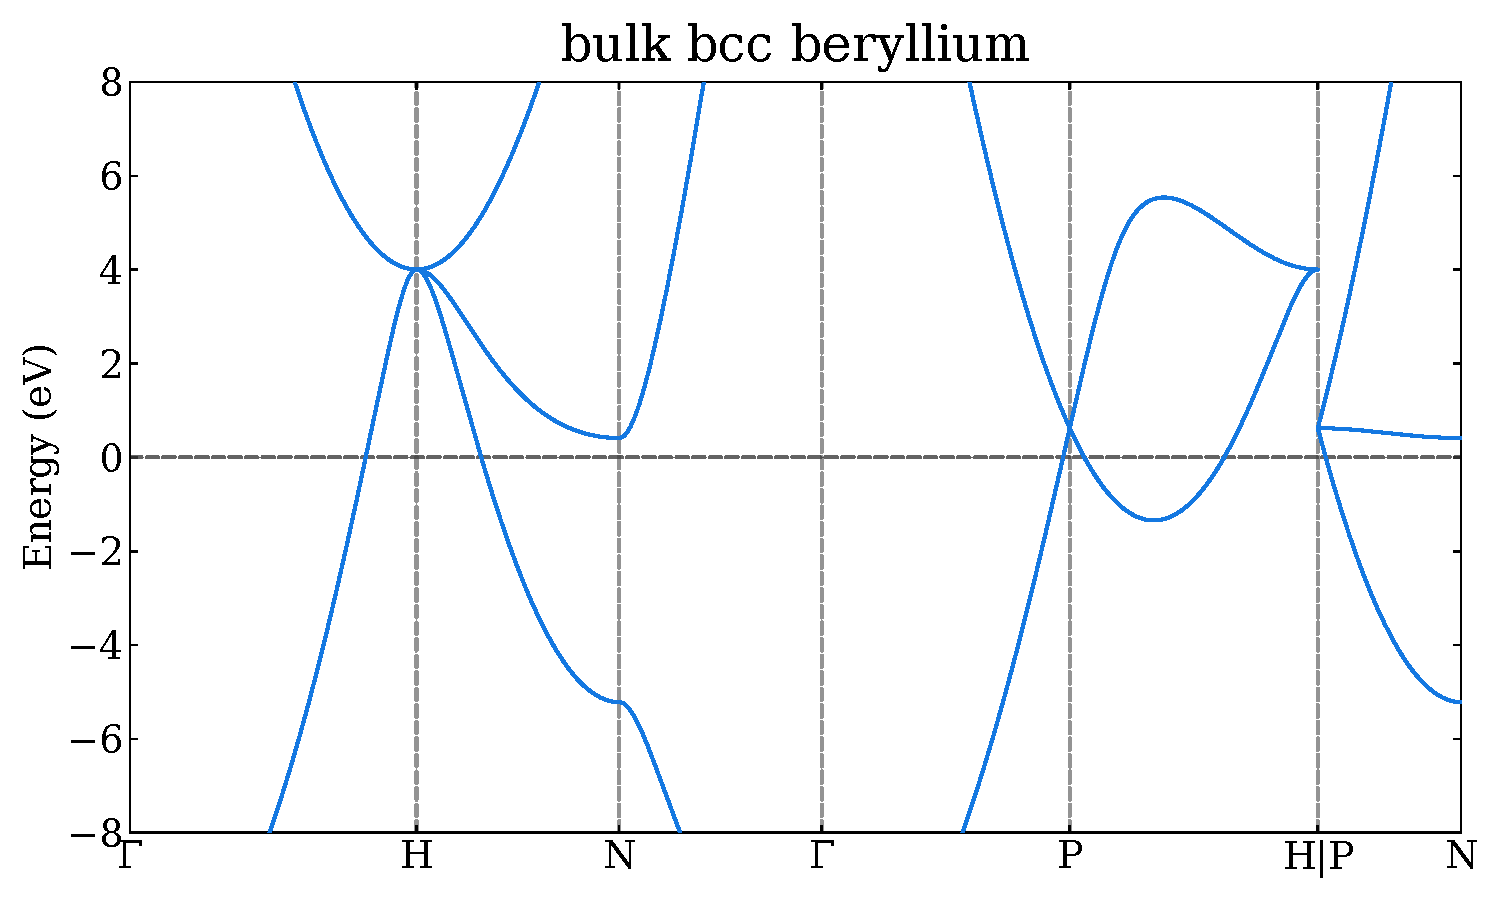
\includegraphics[width=0.40\linewidth]{figures_proj3/bands_bcc-beryllium_thesis.pdf}&
    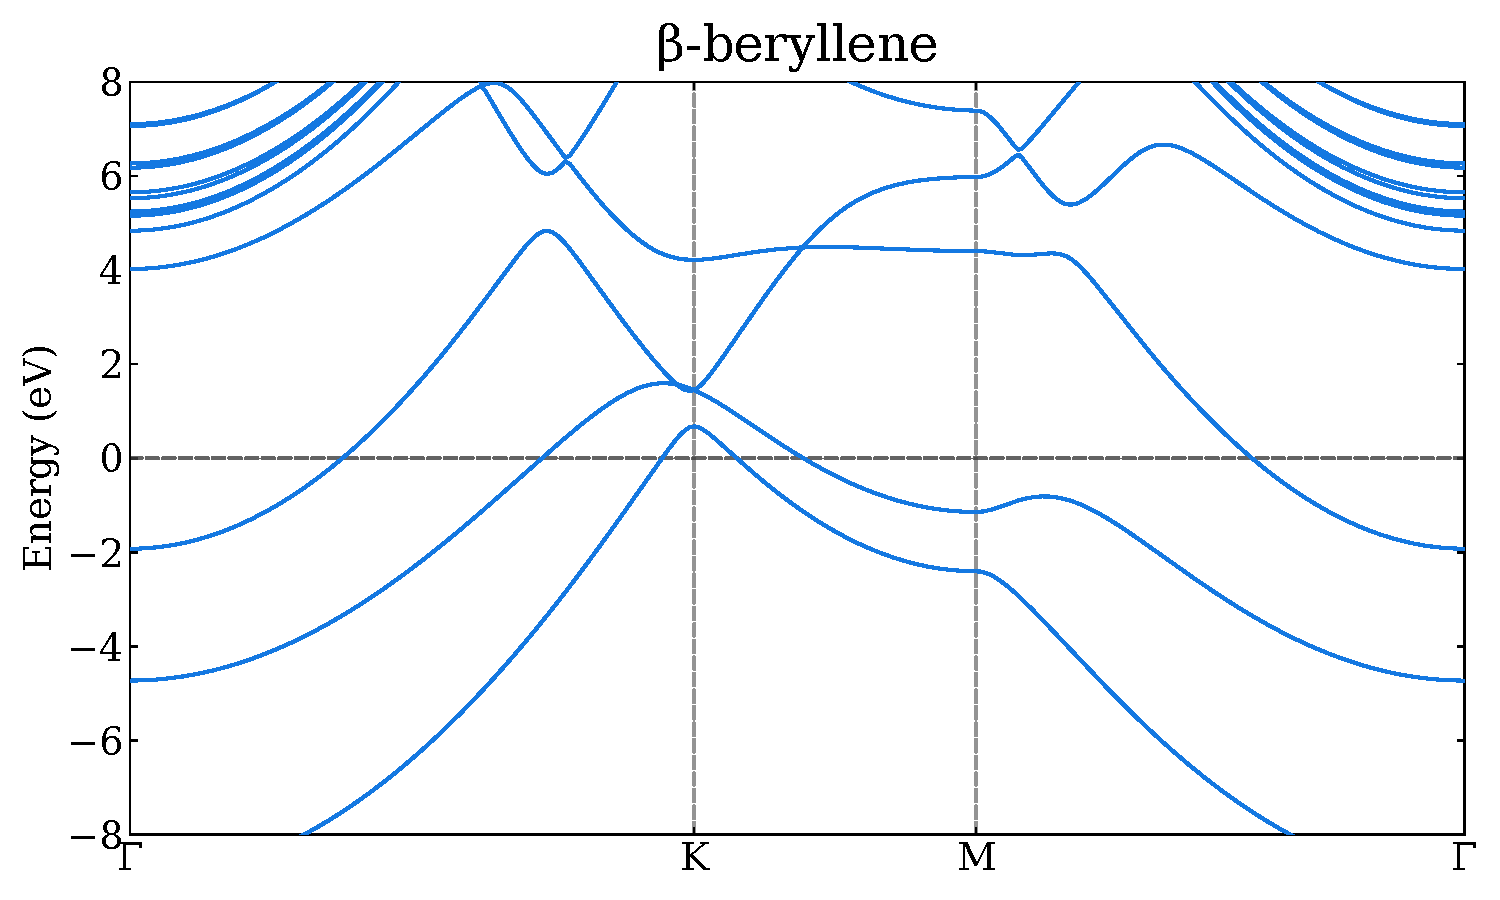
\includegraphics[width=0.40\linewidth]{figures_proj3/bands_beta-beryllene_thesis.pdf}
\end{tabular}
\caption{Band structures of bulk hcp beryllium, $\alpha$-beryllene, bulk bcc beryllium, and $\beta$-beryllene.}
\label{fig:proj3_band_structures}
\end{figure}

\subsection*{Soft mode of 2H-$\beta$-beryllene}

The soft mode of 2H-$\beta$-beryllene lies at the wave vector $\vec{q}=(-0.4,0.4)$ on the $\Gamma$--$\mathrm{M}$ line,
in units of the reciprocal lattice vectors,
which is commensurate with the $5 \times 5$ phonon supercell.
For the frozen-phonon calculations,
we use a 20-atom supercell with lattice vectors $\vec{A}_{1}=5\vec{a}_{1}$ and $\vec{A}_{2}=\vec{a}_{1}+\vec{a}_{2}$,
which is also commensurate with this wave vector.
The atoms are displaced along the eigenvector of the soft mode,
with maximum displacements of \qty{0.025}{\angstrom}, \qty{0.049}{\angstrom}, and \qty{0.098}{\angstrom},
and the total energy is calculated at each amplitude without further relaxation.
We repeat these calculations with Gaussian smearing of \qty{0.02}{\electronvolt}, \qty{0.05}{\electronvolt}, and \qty{0.10}{\electronvolt},
using k-point meshes of $16 \times 97 \times 1$ for \qty{0.02}{\electronvolt} and $11 \times 65 \times 1$ otherwise.
The energies are fitted to $E(Q)-E(0)=aQ^{2}+bQ^{4}$,
where $Q$ is the mass-weighted amplitude of the mode.
The curvature $a$ gives the harmonic frequency,
and $a^{2}/4b$ gives the depth of the double well for $a<0$.
The fitted harmonic frequencies of $1.0\mathrm{i}$--$1.8\mathrm{i}$~\si{\tera\hertz} are comparable with the value of $1.65\mathrm{i}$~\si{\tera\hertz} from the phonon calculation.

To estimate the effect of quantum fluctuations,
we solve the one-dimensional Schr\"odinger equation for the fitted potential numerically.
We also calculate the self-consistent harmonic frequency $\Omega$ of this single mode,
which satisfies $\Omega^{2}=2a+12b\langle Q^{2}\rangle$,
with $\langle Q^{2}\rangle=(\hbar/2\Omega)\coth(\hbar\Omega/2\kB T)$.
The coupling to the other phonon modes is neglected,
so these values indicate the size of the quantum fluctuations.
The results are listed in table~\ref{tab:proj3_soft_mode}.
For all three smearing values,
the ground state lies approximately \qty{6}{\milli\electronvolt} above the bottom of the double well,
far above the well depth,
and the first excitation energy corresponds to approximately \qty{4}{\tera\hertz}.
The root-mean-square amplitude of the ground state,
0.35--0.36~amu$^{1/2}$\,\AA,
exceeds the position of the potential minimum,
0.14--0.24~amu$^{1/2}$\,\AA.
For a smearing of \qty{0.02}{\electronvolt},
the maximum fit residual of \qty{0.16}{\milli\electronvolt} is comparable to the fitted well depth,
so this depth is only an upper estimate.

\begin{table}[!htbp]
\centering
\rowcolors{2}{gray!15}{white}
\begin{adjustbox}{center,max width=1.0\linewidth}
\begin{tabular}{lccc}
\hline
\rowcolor{gray!25}
Gaussian smearing (eV) & 0.02 & 0.05 & 0.10 \\
supercell k-point mesh & $16 \times 97 \times 1$ & $11 \times 65 \times 1$ & $11 \times 65 \times 1$ \\
\hline
$\Delta E$ at \qty{0.025}{\angstrom} (meV) & $0.015$ & $-0.013$ & $-0.012$ \\
$\Delta E$ at \qty{0.049}{\angstrom} (meV) & $-0.007$ & $0.578$ & $0.495$ \\
$\Delta E$ at \qty{0.098}{\angstrom} (meV) & $10.029$ & $12.450$ & $11.932$ \\
fitted harmonic frequency (THz) & $1.75\mathrm{i}$ & $1.02\mathrm{i}$ & $1.13\mathrm{i}$ \\
double-well depth (meV) & $0.185$ & $0.021$ & $0.032$ \\
maximum fit residual (meV) & $0.158$ & $0.001$ & $0.018$ \\
\hline
ground state above the well bottom (meV) & $5.88$ & $6.31$ & $6.21$ \\
first excitation energy (THz) & $3.77$ & $4.00$ & $3.95$ \\
self-consistent frequency at \qty{0}{\kelvin} (THz) & $4.03$ & $4.23$ & $4.18$ \\
self-consistent frequency at \qty{300}{\kelvin} (THz) & $5.54$ & $5.67$ & $5.63$ \\
\hline
\end{tabular}
\end{adjustbox}
\caption{Frozen-phonon energies $\Delta E$ of the soft mode of 2H-$\beta$-beryllene relative to the undistorted structure,
per 20-atom supercell and at the given maximum atomic displacements,
parameters of the quartic fit,
and the one-mode quantum estimates.}
\label{tab:proj3_soft_mode}
\end{table}

The bare static susceptibility and the nesting function of 2H-$\beta$-beryllene are shown in figure~\ref{fig:proj3_nesting}.
Neither quantity has a peak at the soft-mode wave vector,
so the softening is not driven by Fermi-surface nesting.

\begin{figure}[!htbp]
\centering
    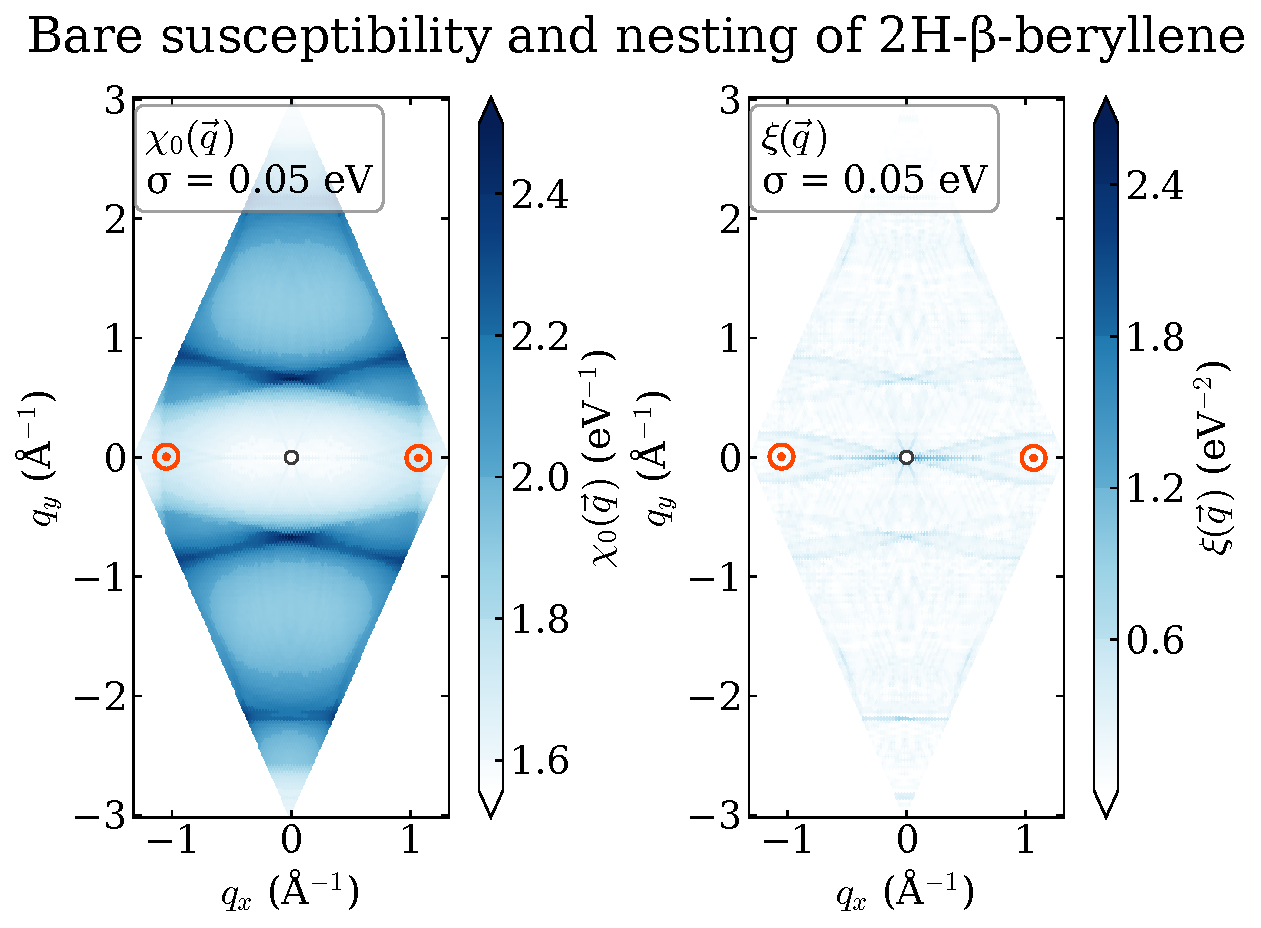
\includegraphics[width=0.80\linewidth]{figures_proj3/nesting_2H-beta-beryllene_thesis.pdf}
\caption{Bare static susceptibility $\chi_{0}(\vec{q}\,)$ (left) and nesting function $\xi(\vec{q}\,)$ (right) of 2H-$\beta$-beryllene,
calculated with constant matrix elements from the spin-orbit-coupled eigenvalues on the $105 \times 105$ mesh,
with Gaussian smearing of \qty{0.05}{\electronvolt}.
The bands with states within \qty{1}{\electronvolt} of the Fermi level are included.
The open circles mark the soft-mode wave vector and its symmetry images,
and the value at $\vec{q}=0$ is excluded from the colour scale.
Among the 11024 non-zero wave vectors of the mesh,
the soft-mode wave vector ranks between 8723 and 8935 in $\chi_{0}$ and between 3806 and 8405 in $\xi$ for smearing between 0.02 and \qty{0.10}{\electronvolt}.}
\label{fig:proj3_nesting}
\end{figure}

\subsection*{Hydrogenation energetics}

The adsorption energies of hydrogen relative to \ce{H2} are listed in table~\ref{tab:proj3_hydrogenation_energetics},
together with the zero-point energy and finite-temperature corrections.
The zero-point energies of the beryllene layers are calculated from the harmonic phonons on a $40 \times 40$ q-point mesh,
and the zero-point energy of \ce{H2} is \qty{0.269}{\electronvolt}.
The free energies at \qty{298.15}{\kelvin} and \qty{1}{\bar} include the harmonic vibrational free energies of the layers
and the enthalpy and entropy of gaseous \ce{H2},
$H(T)-H(0)-TS=\qty{-0.316}{\electronvolt}$ per \ce{H2}.
The equilibrium \ce{H2} pressure is the pressure at which the adsorption free energy vanishes,
$p_{\mathrm{eq}}=p^{\circ}\exp\left(2\Delta G/\kB T\right)$ with $p^{\circ}=\qty{1}{\bar}$.
The zero-point energy raises all adsorption energies by \qtyrange{0.08}{0.09}{\electronvolt} per hydrogen atom,
because the vibrations of the adsorbed hydrogen atoms outweigh the stretching mode of \ce{H2}.
For 2H-$\beta$-beryllene,
the imaginary phonon modes are excluded from the vibrational free energy.
They cover \qty{1.1}{\percent} of the Brillouin zone,
and their contribution is below \qty{0.1}{\milli\electronvolt} per hydrogen atom.

\begin{table}[!htbp]
\centering
\rowcolors{2}{gray!15}{white}
\begin{tabular}{ccccc}
\hline
\rowcolor{gray!25}
structure
& $\Delta E$ (eV)
& $\Delta E+\Delta E_{\mathrm{ZPE}}$ (eV)
& $\Delta G$ (eV)
& $p_{\mathrm{eq}}$ (bar) \\
\hline
2H-$\alpha$-beryllene & $-0.331$ & $-0.243$ & $-0.084$ & $1.4\times10^{-3}$ \\
1H-$\beta$-beryllene & $-0.072$ & $0.012$ & $0.166$ & $4.0\times10^{5}$ \\
2H-$\beta$-beryllene & $-0.173$ & $-0.090$ & $0.058$ & $93$ \\
\hline
\end{tabular}
\caption{Adsorption energy per hydrogen atom relative to \ce{H2},
$\Delta E$,
the same energy including the zero-point energy correction,
$\Delta E+\Delta E_{\mathrm{ZPE}}$,
the adsorption free energy per hydrogen atom at \qty{298.15}{\kelvin} and \qty{1}{\bar},
$\Delta G$,
and the equilibrium \ce{H2} pressure at \qty{298.15}{\kelvin},
$p_{\mathrm{eq}}$.}
\label{tab:proj3_hydrogenation_energetics}
\end{table}

The relaxed energies of the \ce{BeH2} monolayers are listed in table~\ref{tab:proj3_beh2_polymorphs}.
All four structures are relaxed with the same settings as 2H-$\alpha$-beryllene,
and their space groups are determined with a tolerance of \qty{1e-3}{\angstrom}.
When the hydrogen atoms on the two sides occupy aligned hollow sites,
the layer relaxes to a $Cmmm$ structure that is \qty{0.74}{\electronvolt} per formula unit higher in energy.
The dynamical stability of the puckered square layer is not calculated.

\begin{table}[!htbp]
\centering
\rowcolors{2}{gray!15}{white}
\begin{adjustbox}{center,max width=1.0\linewidth}
\begin{tabular}{cccc}
\hline
\rowcolor{gray!25}
structure & space group & Be-H coordination & $\Delta E$ (meV per \ce{BeH2}) \\
\hline
2H-$\alpha$-beryllene, staggered hollows & $P\bar{3}m1$ & 6 H at \qty{1.599}{\angstrom} & $0$ \\
2H-$\alpha$-beryllene, aligned hollows & $Cmmm$ & 4 H at \qty{1.488}{\angstrom} & $740.6$ \\
puckered square layer & $P\bar{4}m2$ & 4 H at \qty{1.468}{\angstrom} & $-38.2$ \\
planar square layer & $P4/mmm$ & 4 H at \qty{1.479}{\angstrom} & $1233.1$ \\
\hline
\end{tabular}
\end{adjustbox}
\caption{Space groups,
coordination of beryllium by hydrogen,
and relaxed total energies per formula unit relative to 2H-$\alpha$-beryllene for the \ce{BeH2} monolayers considered.}
\label{tab:proj3_beh2_polymorphs}
\end{table}

\subsection*{Topological screening}

The direct gaps $E_{N+1}-E_{N}$ between the lowest $N$ spinor bands and band $N+1$ are shown over the Brillouin zone in figures~\ref{fig:proj3_direct_gap_pristine} and~\ref{fig:proj3_direct_gap_hydrogenated}.
We unfold the $105 \times 105$ mesh of the self-consistent calculation with the symmetry operations of each structure,
and refine the minima of the direct gap on locally denser meshes with non-self-consistent spin-orbit calculations.
For the pristine structures,
the smallest direct gaps are approximately \qty{1}{\milli\electronvolt},
so each local minimum is further refined with successively smaller $9 \times 9$ patches,
as shown in figure~\ref{fig:proj3_gap_zoom}.
The minima of $\alpha$- and $\beta$-beryllene remain at $\mathrm{K}$ over four refinement levels,
and the minimum of trilayer cubic beryllene remains on the $\Gamma$--$\mathrm{M}$ line over five levels.
In each case,
the lower bound obtained by subtracting the largest local slope times the sampling radius from the minimum gap remains positive,
between 0.65 and \qty{1.07}{\milli\electronvolt}.
The local refinements locate minima at fixed self-consistent charge density.
The convergence of these meV gaps with respect to the plane-wave cutoff and the self-consistent k-point mesh has not been tested separately from the total-energy convergence.
The smallest direct gap of the hydrogen-functionalized structures is \qty{0.177}{\electronvolt}.
The Wannier charge centres of 1H-$\beta$-beryllene are shown in figure~\ref{fig:proj3_wcc}.
For both the lowest four and the lowest six bands,
the Wannier charge centres are crossed an even number of times by any reference line over half of the Brillouin zone,
which gives $\nu=0$.

The parities obtained with the HSE06 hybrid functional without spin-orbit coupling are compared with the PBE results in table~\ref{tab:proj3_hse_parity}.
The numbers of odd-parity states among the lowest $N/2$ spinless bands agree with the numbers of odd-parity Kramers pairs in PBE with spin-orbit coupling at all four time-reversal invariant momenta.
The parity products at these momenta are therefore unchanged.
This comparison checks the parity ordering at these momenta.
The isolation of the lowest-$N$ spinor subspaces throughout the Brillouin zone with HSE06 and spin-orbit coupling is a separate test.
For 2H-$\beta$-beryllene,
the gap above band 6 at $\mathrm{M}$ is \qty{0.171}{\electronvolt} with HSE06 and \qty{0.178}{\electronvolt} with PBE in the same cell.

The time-reversal symmetry assumed in the analysis is supported by several checks.
The converged spin-orbit-coupled states have a maximum magnetization density below $3\times10^{-7}~\mu_{\mathrm{B}}\,\text{\AA}^{-3}$,
and the Kramers splittings at the time-reversal invariant momenta are at most \qty{3.8e-6}{\electronvolt}.
For 1H-$\beta$-beryllene,
which has no inversion symmetry,
the eigenvalues satisfy $E(\vec{k}\,)=E(-\vec{k}\,)$ within \qty{4.0e-7}{\electronvolt} for all 5512 pairs of wave vectors on the mesh.
All 11 spin-polarized calculations started from ferromagnetic,
antiferromagnetic,
and,
for trilayer cubic beryllene,
inversion-odd magnetic configurations converge to the non-magnetic state,
with all site moments below $10^{-3}~\mu_{\mathrm{B}}$.

\begin{table}[!htbp]
\centering
\rowcolors{2}{gray!15}{white}
\begin{adjustbox}{max width=1.0\linewidth,center}
\begin{tabular}{ccccc}
\hline
\rowcolor{gray!25}
structure
& $N$
& odd pairs at $\Gamma$, $\mathrm{X}$, $\mathrm{Y}$, $\mathrm{M}$
& $\nu$
& smallest gap (eV), HSE06 / PBE \\
\hline
$\alpha$-beryllene & 2 & 0, 1, 1, 1 & 1 & $\Gamma$: 6.209 / 5.169 \\
$\beta$-beryllene & 4 & 1, 1, 1, 1 & 0 & $\Gamma$: 3.471 / 2.795 \\
trilayer cubic beryllene & 6 & 1, 1, 1, 2 & 1 & $\mathrm{M}$: even-parity doublet \\
2H-$\alpha$-beryllene & 4 & 1, 1, 1, 1 & 0 & $\mathrm{X}$: 6.847 / 5.644 \\
2H-$\beta$-beryllene & 6 & 1, 1, 2, 2 & 0 & $\mathrm{M}$: 0.171 / 0.178 \\
\hline
\end{tabular}
\end{adjustbox}
\caption{Numbers of odd-parity Kramers pairs among the lowest $N$ bands at the time-reversal invariant momenta,
$\mathbb{Z}_2$ indices,
and smallest gaps $E_{N+1}-E_{N}$ at the time-reversal invariant momenta.
The HSE06 counts use the lowest $N/2$ spinless states,
whose parities agree with those of the PBE Kramers pairs.
The listed $\mathbb{Z}_2$ indices are conditional PBE results with spin-orbit coupling.
The HSE06 and PBE gaps are calculated in the same \qty{20}{\angstrom} cell without spin-orbit coupling.
For trilayer cubic beryllene,
the boundary of the lowest six bands at $\mathrm{M}$ lies within an orbital doublet of even parity,
which is split only by spin-orbit coupling.}
\label{tab:proj3_hse_parity}
\end{table}

\begin{figure}[!htbp]
\centering
    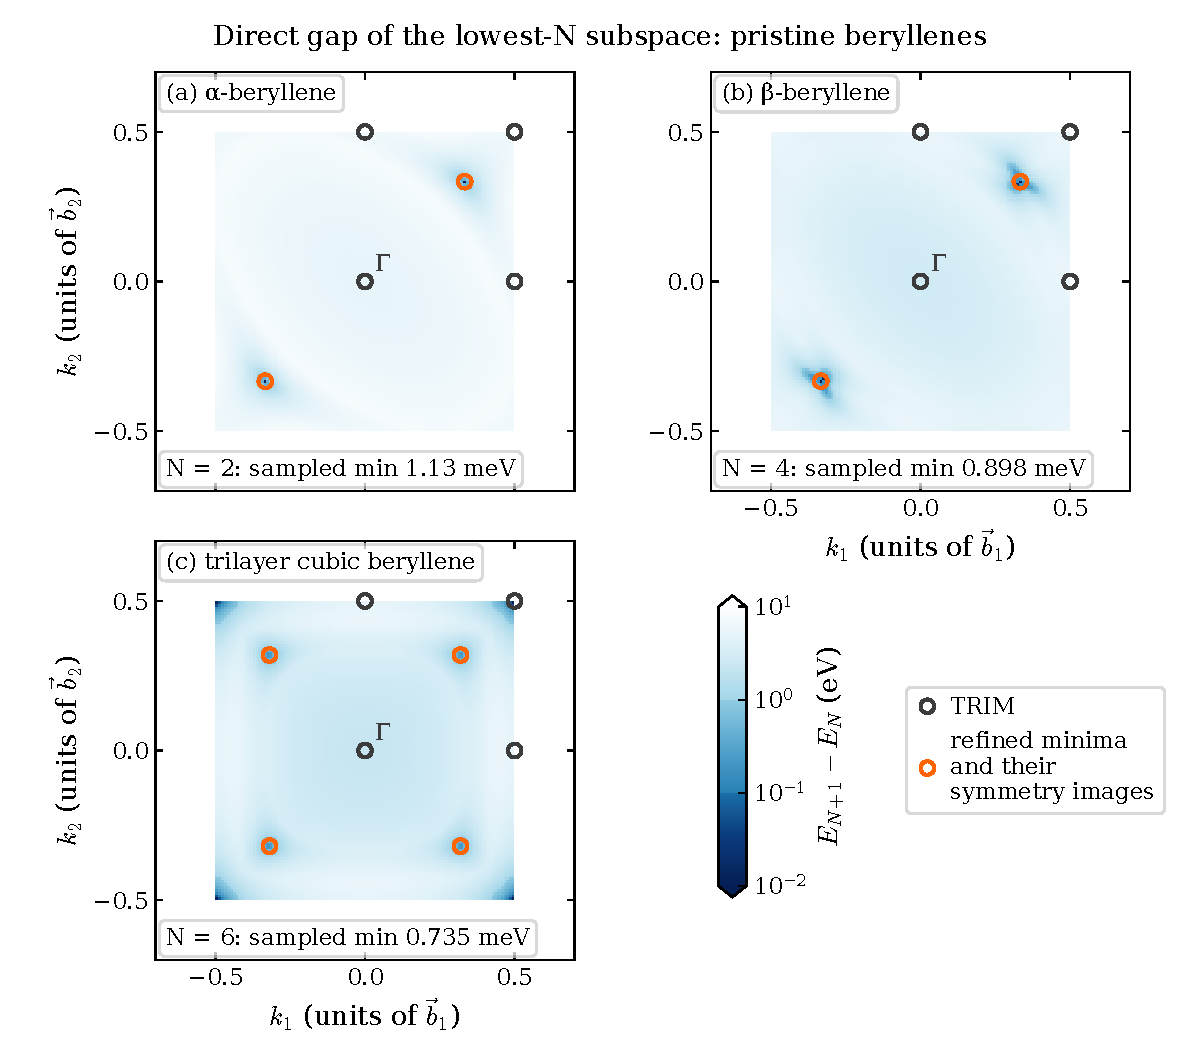
\includegraphics[width=0.80\linewidth]{figures_proj3/topology_direct-gap_pristine_thesis.pdf}
\caption{Direct gap $E_{N+1}-E_{N}$ of the lowest-$N$ subspace over the Brillouin zone for (a) $\alpha$-beryllene,
(b) $\beta$-beryllene,
and (c) trilayer cubic beryllene,
on a logarithmic scale.
The time-reversal invariant momenta,
the refined minima,
and their symmetry images are marked.}
\label{fig:proj3_direct_gap_pristine}
\end{figure}

\begin{figure}[!htbp]
\centering
    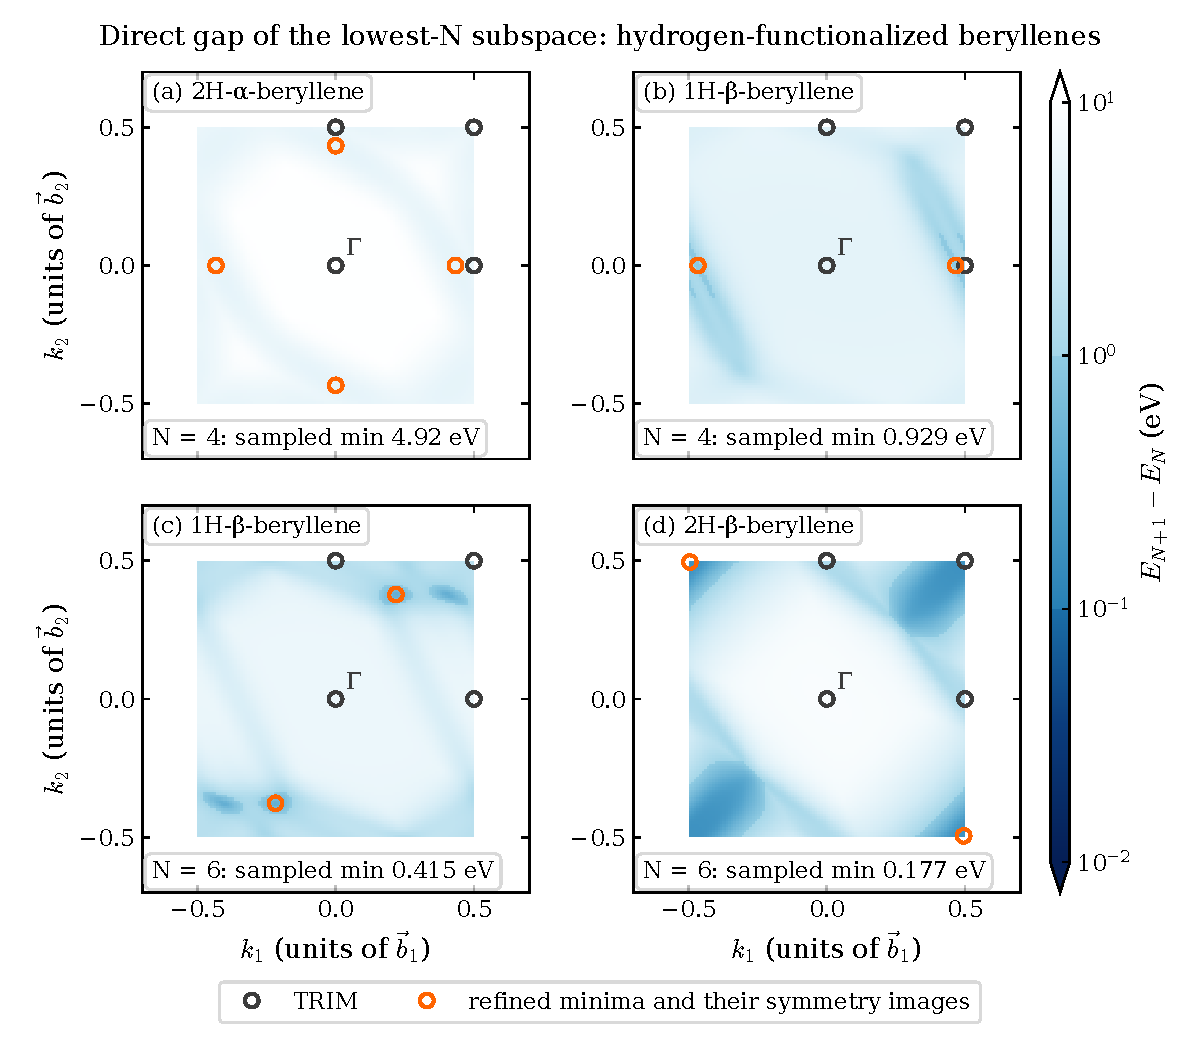
\includegraphics[width=0.80\linewidth]{figures_proj3/topology_direct-gap_hydrogenated_thesis.pdf}
\caption{Direct gap $E_{N+1}-E_{N}$ of the lowest-$N$ subspace over the Brillouin zone for (a) 2H-$\alpha$-beryllene,
(b, c) 1H-$\beta$-beryllene with $N=4$ and $N=6$,
and (d) 2H-$\beta$-beryllene,
shown as in figure~\ref{fig:proj3_direct_gap_pristine}.}
\label{fig:proj3_direct_gap_hydrogenated}
\end{figure}

\begin{figure}[!htbp]
\centering
    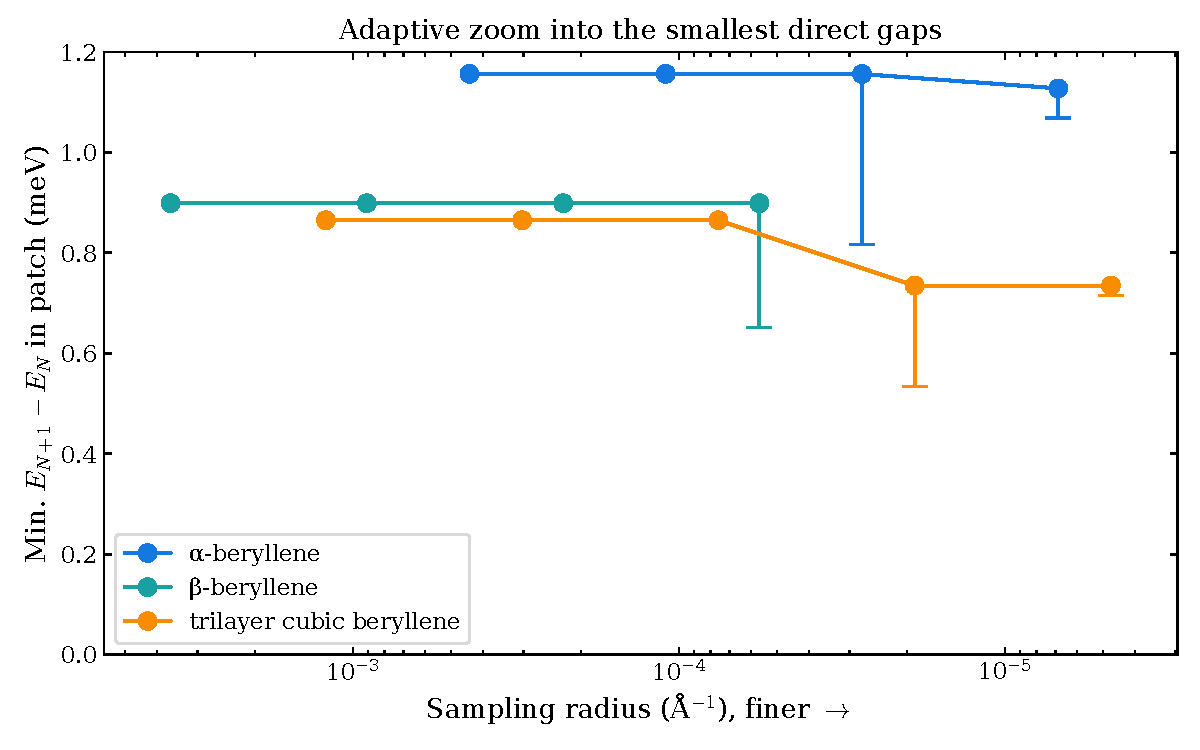
\includegraphics[width=0.80\linewidth]{figures_proj3/topology_gap-zoom_thesis.pdf}
\caption{Minimum direct gap in each refinement patch as a function of the sampling radius for $\alpha$-beryllene,
$\beta$-beryllene,
and trilayer cubic beryllene.
The lower ends of the vertical bars show the lower bounds estimated from the local slope of the gap.}
\label{fig:proj3_gap_zoom}
\end{figure}

\begin{figure}[!htbp]
\centering
    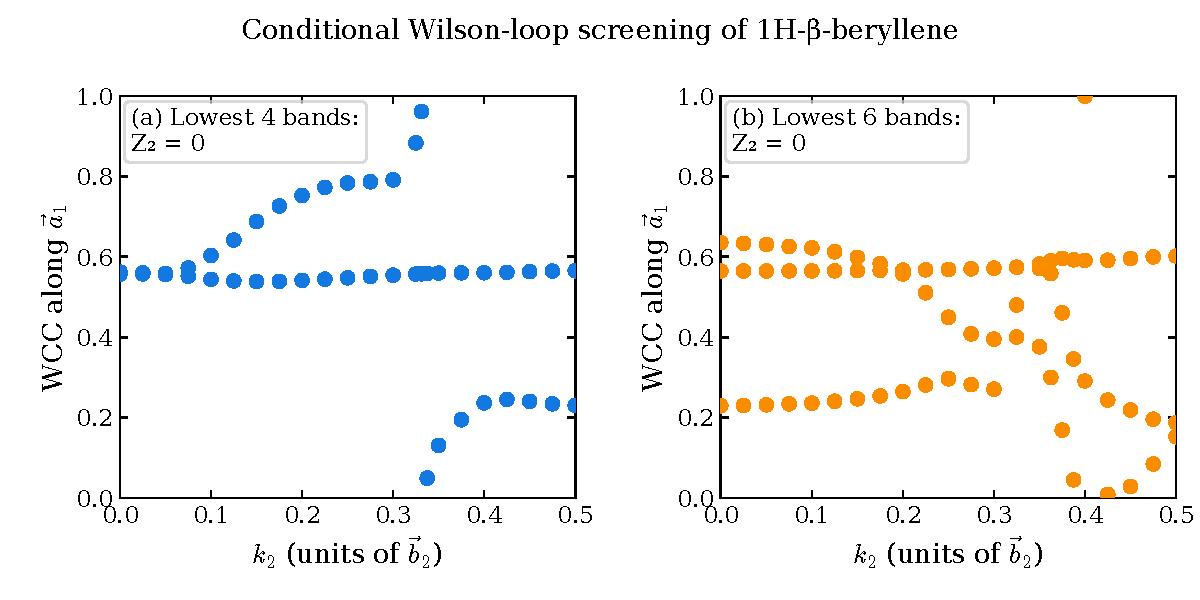
\includegraphics[width=0.80\linewidth]{figures_proj3/topology_wcc_1H-beta-beryllene_thesis.pdf}
\caption{Wannier charge centres of 1H-$\beta$-beryllene along $\vec{a}_{1}$ as functions of $k_{2}$ over half of the Brillouin zone,
for (a) the lowest four bands and (b) the lowest six bands.}
\label{fig:proj3_wcc}
\end{figure}

\subsection*{Structures for the \texttt{Quantum ESPRESSO} calculations}

The structures optimized with PBE in \texttt{Quantum ESPRESSO},
which are used for the topological cross-check and the electron-phonon calculations,
are listed in table~\ref{tab:proj3_qe_structures}.
For 2H-$\beta$-beryllene,
the phonon and electron-phonon calculations instead use the structure relaxed with the D3 dispersion correction,
listed in the last row of the table.
In \texttt{Quantum ESPRESSO} with this correction,
the residual forces on this structure are below \qty{0.03}{\electronvolt\per\angstrom}.

\begin{table}[!htbp]
\centering
\rowcolors{2}{gray!15}{white}
\begin{adjustbox}{max width=1.0\linewidth,center}
\begin{tabular}{ccccccc}
\hline
\rowcolor{gray!25}
system
& cell content
& $a$
& $b$
& angle
& thickness
& electronic nature \\
\hline
trilayer cubic beryllene
& \ce{Be3} & 2.18 & 2.18 & $90.00^{\circ}$ & 3.04 & metallic \\
2H-$\alpha$-beryllene
& \ce{BeH2} & 2.32 & 2.32 & $120.00^{\circ}$ & 1.74 & semiconductor \\
2H-$\beta$-beryllene
& \ce{Be2H2} & 2.62 & 2.62 & $133.12^{\circ}$ & 3.78 & metallic \\
1H-$\beta$-beryllene
& \ce{Be2H} & 2.32 & 2.11 & $117.01^{\circ}$ & 2.85 & metallic \\
\hline
2H-$\beta$-beryllene, PBE+D3
& \ce{Be2H2} & 2.53 & 2.53 & $131.88^{\circ}$ & 3.79 & metallic \\
\hline
\end{tabular}
\end{adjustbox}
\caption{Cell content,
lattice constants $a$ and $b$,
angle between the two in-plane lattice vectors,
thickness between the outermost atomic centres,
and electronic nature of the structures optimized with PBE in \texttt{Quantum ESPRESSO}.
The last row is the structure relaxed with the D3 dispersion correction,
which is used for the phonon and electron-phonon calculations of 2H-$\beta$-beryllene.
The lattice constants and thickness are given in \si{\angstrom}.}
\label{tab:proj3_qe_structures}
\end{table}

\subsection*{Phonon and electron-phonon calculations}

On the $12 \times 12 \times 1$ q-point mesh,
the phonon frequencies from density functional perturbation theory are real for all three structures,
except at $\Gamma$,
where the lowest values are $0.14\mathrm{i}$~\si{\tera\hertz},
$0.24\mathrm{i}$~\si{\tera\hertz},
and $0.20\mathrm{i}$~\si{\tera\hertz} for trilayer cubic beryllene,
2H-$\beta$-beryllene,
and 1H-$\beta$-beryllene,
respectively.
The Wannier interpolation uses 12, 10, and 9 Wannier functions for these three structures,
with frozen windows that extend to \qtyrange{3.0}{3.6}{\electronvolt} above the Fermi level.

The electron-phonon coupling of trilayer cubic beryllene and 2H-$\beta$-beryllene depends on the lower phonon frequency threshold,
as shown in table~\ref{tab:proj3_epw_threshold} and figure~\ref{fig:proj3_a2f}.
With a threshold of \qty{5}{\per\centi\metre} on the $40 \times 40 \times 1$ fine meshes,
the modes below \qty{40}{\per\centi\metre} contribute approximately half of $\lambda$ for these two structures.
Restricting the same spectral functions to frequencies above \qty{40}{\per\centi\metre} gives $\lambda=0.44$ and $\lambda=1.50$,
close to the values on the $80 \times 80 \times 1$ fine meshes.
For 1H-$\beta$-beryllene,
both fine meshes use the threshold of \qty{5}{\per\centi\metre} and give similar values.

\begin{table}[!htbp]
\centering
\rowcolors{2}{gray!15}{white}
\begin{adjustbox}{max width=1.0\linewidth,center}
\begin{tabular}{cccccc}
\hline
\rowcolor{gray!25}
structure
& fine meshes
& threshold (\si{\per\centi\metre})
& $\lambda$
& $\hbar\omega_\mathrm{log}$ (meV)
& $T_\mathrm{c}^{\mathrm{AD}}$ (K) \\
\hline
trilayer cubic beryllene & $40 \times 40 \times 1$ & 5 & 1.00 & 4.0 & 2.8 \\
trilayer cubic beryllene & $80 \times 80 \times 1$ & 40 & 0.46 & 36.0 & 2.0 \\
2H-$\beta$-beryllene & $40 \times 40 \times 1$ & 5 & 3.06 & 7.5 & 15.1 \\
2H-$\beta$-beryllene & $80 \times 80 \times 1$ & 40 & 1.40 & 19.5 & 21.9 \\
1H-$\beta$-beryllene & $40 \times 40 \times 1$ & 5 & 0.60 & 41.0 & 7.8 \\
1H-$\beta$-beryllene & $80 \times 80 \times 1$ & 5 & 0.61 & 40.7 & 8.1 \\
\hline
\end{tabular}
\end{adjustbox}
\caption{Electron-phonon coupling strength $\lambda$,
logarithmic average frequency $\omega_\mathrm{log}$,
and Allen--Dynes transition temperature $T_\mathrm{c}^{\mathrm{AD}}$ for $\mu^*=0.13$,
calculated with different fine meshes and lower phonon frequency thresholds.}
\label{tab:proj3_epw_threshold}
\end{table}

\begin{figure}[!htbp]
\centering
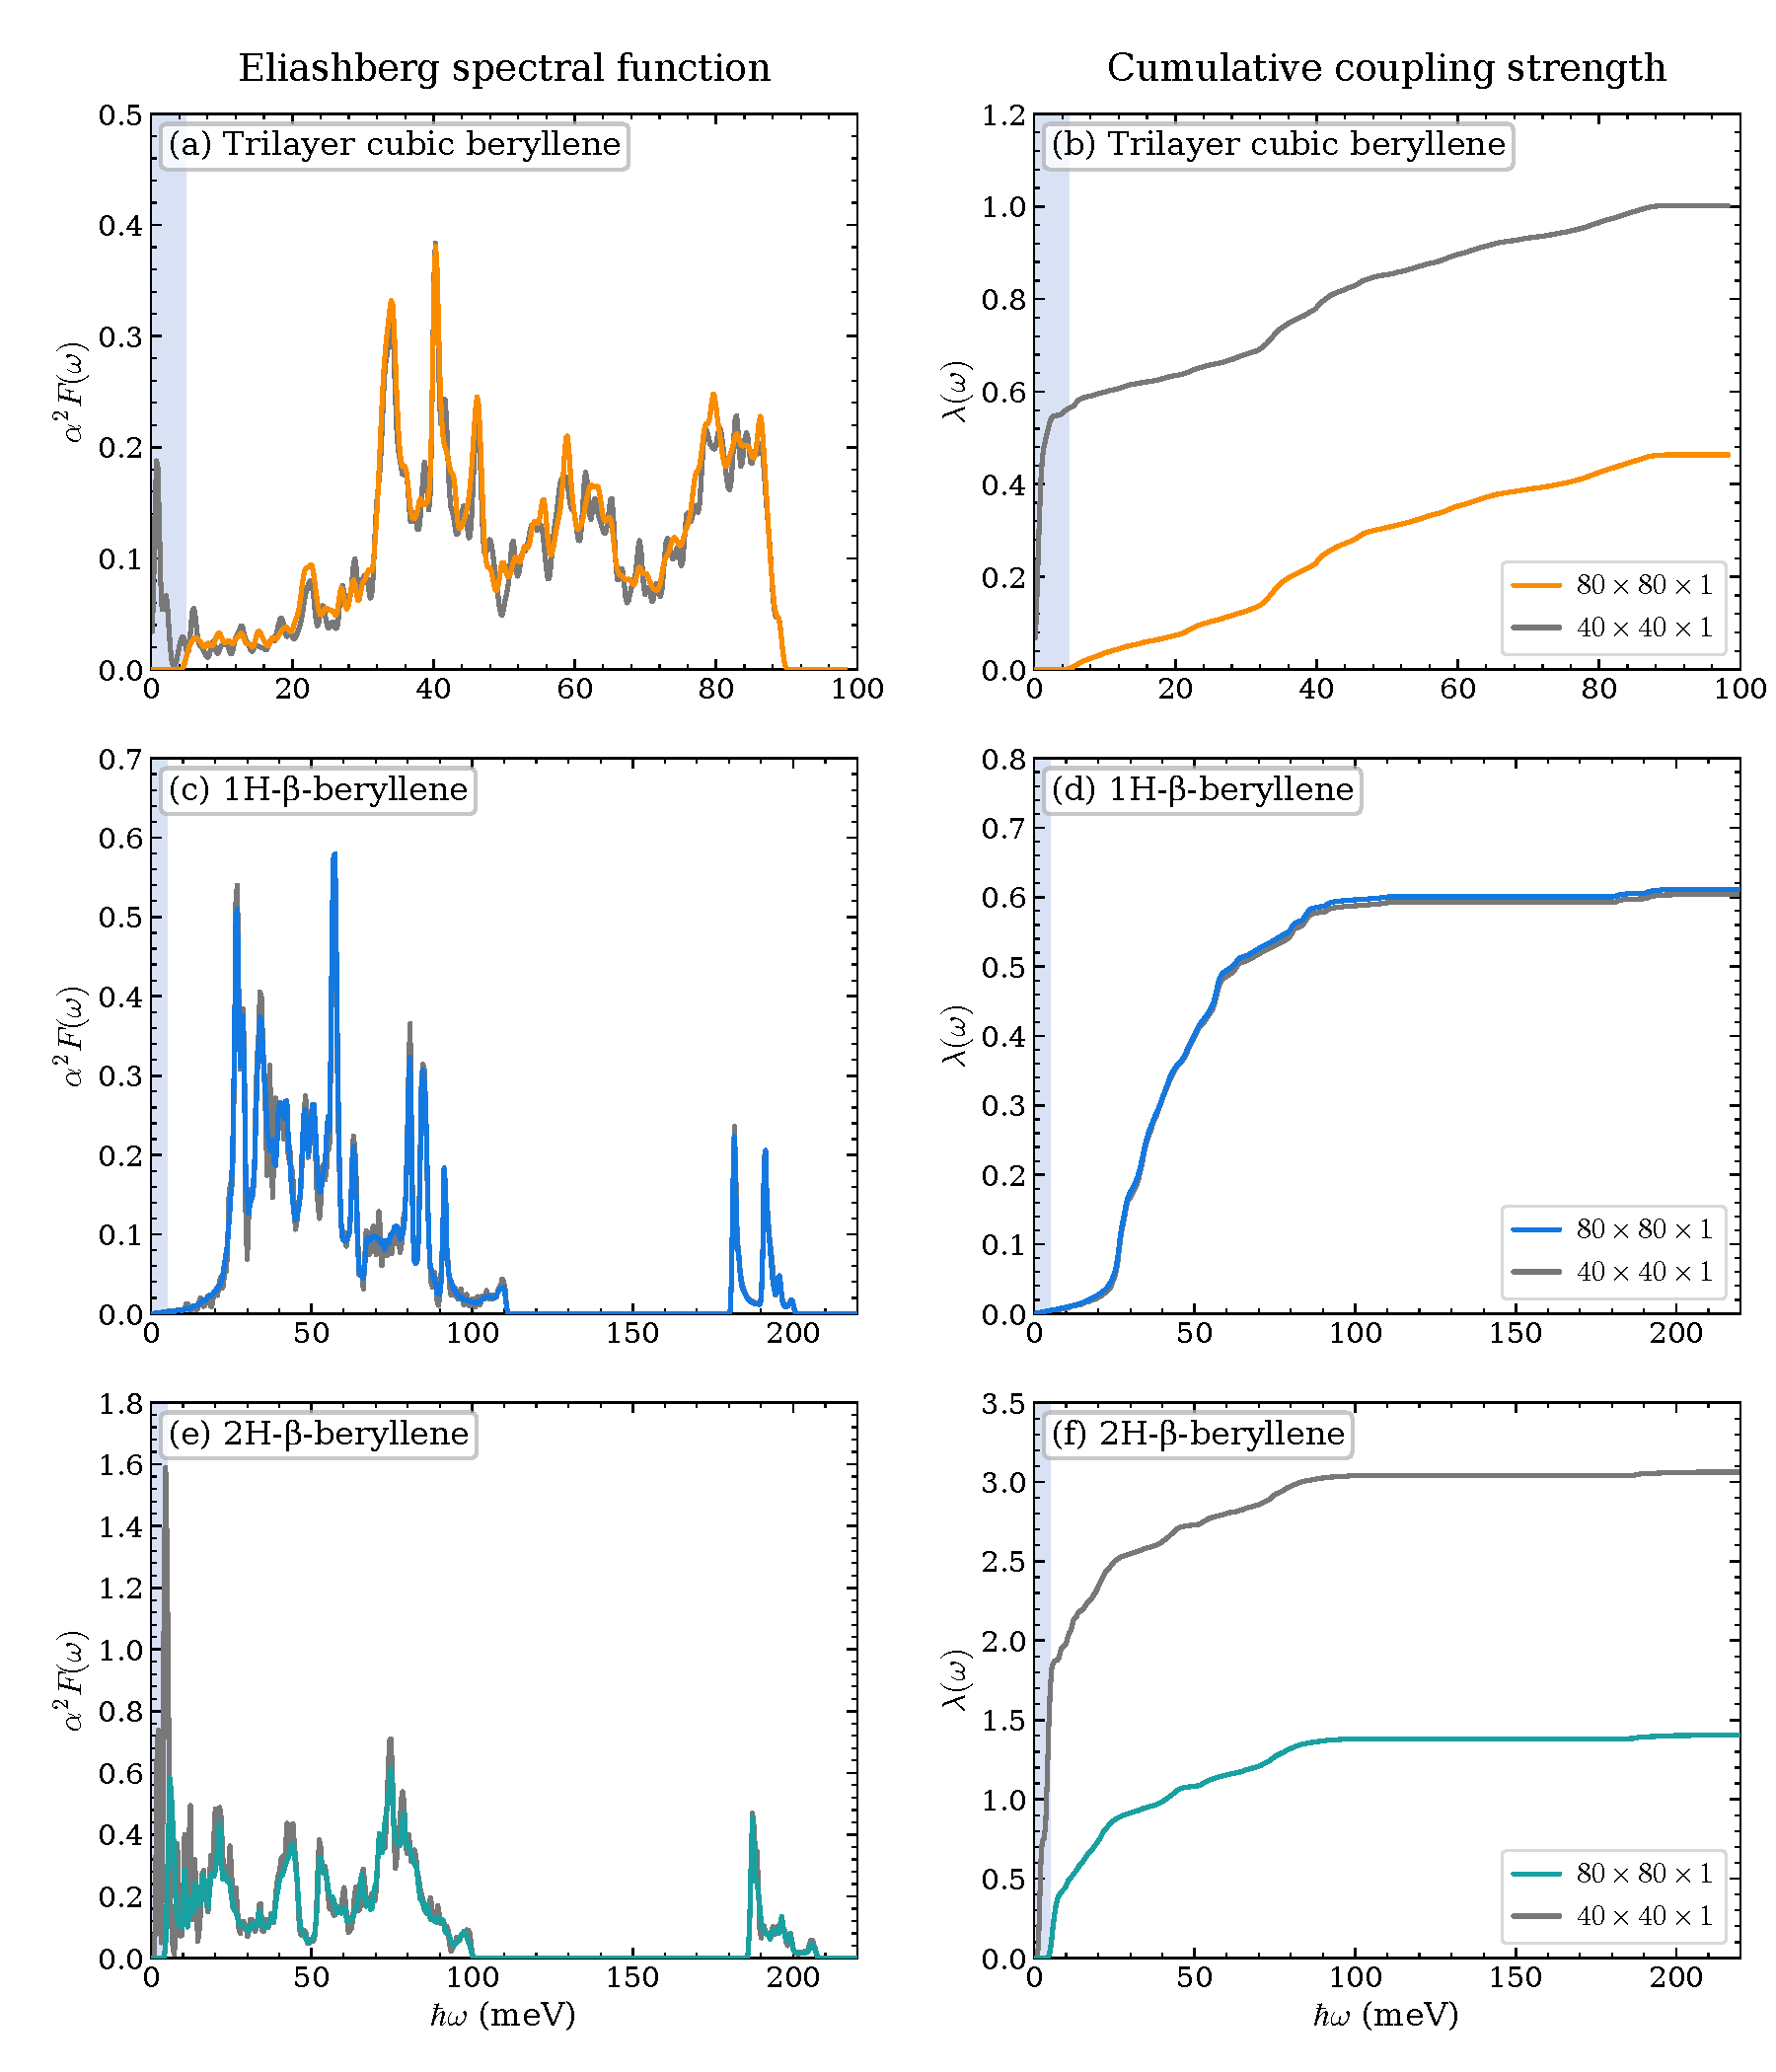
\includegraphics[width=0.80\linewidth]{figures_proj3/superconductivity/superconductivity_a2f.pdf}
\caption{Eliashberg spectral function $\alpha^2F(\omega)$ and cumulative coupling strength $\lambda(\omega)$ of trilayer cubic beryllene, 1H-$\beta$-beryllene, and 2H-$\beta$-beryllene.
(a), (c), and (e) show $\alpha^2F(\omega)$.
(b), (d), and (f) show $\lambda(\omega)$, obtained from equation~\eqref{electron_phonon_spectral_moments} with the integration ending at $\omega$.
Solid lines correspond to the $80 \times 80 \times 1$ fine meshes with the thresholds given in section~\ref{3_methods},
and dashed lines correspond to the $40 \times 40 \times 1$ fine meshes with a threshold of \qty{5}{\per\centi\metre}.
The shaded region marks phonon energies below \qty{40}{\per\centi\metre}.}
\label{fig:proj3_a2f}
\end{figure}

\subsection*{Additional optical spectra}

Additional optical spectra are shown in figures~\ref{fig:proj3_reflectivity_alpha_beta}--\ref{fig:proj3_optical_hydrogenated_extinction}.
Figures~\ref{fig:proj3_reflectivity_alpha_beta} and~\ref{fig:proj3_energy_loss_alpha_beta} show the reflectivity and energy-loss spectrum for $\alpha$-beryllene and $\beta$-beryllene.
Figures~\ref{fig:proj3_optical_clean}--\ref{fig:proj3_optical_clean_extinction} compare the pristine bulk and two-dimensional beryllium structures,
whereas figures~\ref{fig:proj3_optical_hydrogenated}--\ref{fig:proj3_optical_hydrogenated_extinction} compare the corresponding hydrogen-functionalized structures.
These spectra are scalar comparisons derived from the individual Cartesian diagonal components of the dielectric tensor,
following the definitions in section~\ref{3_methods}.
For 1H-$\beta$-beryllene and 2H-$\beta$-beryllene,
off-diagonal dielectric coupling is not included in these scalar quantities.

\begin{figure}[!htbp]
\centering
    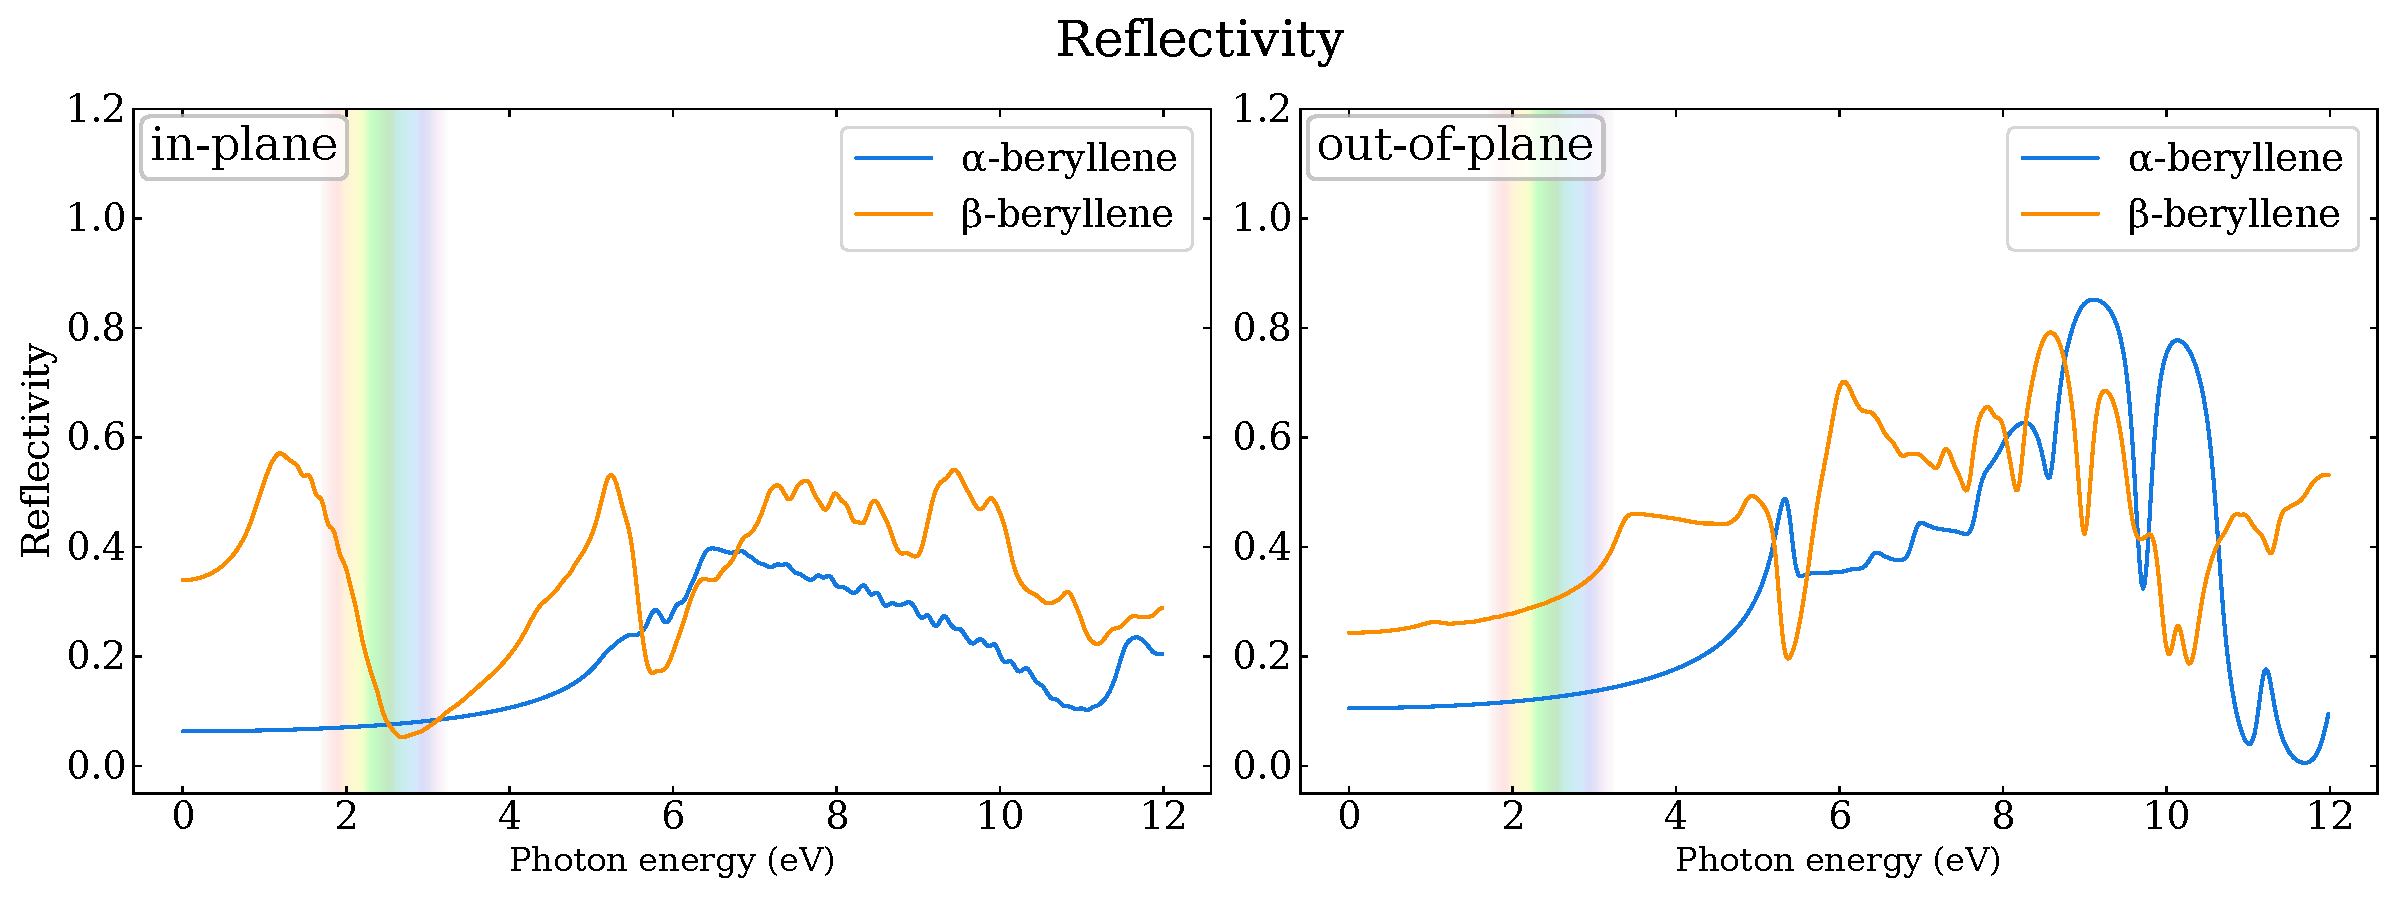
\includegraphics[width=0.80\linewidth]{figures_proj3/optics_alpha-beta_reflectivity_thesis.pdf}
\caption{Reflectivity for the in-plane and out-of-plane directions as a function of photon energy for $\alpha$-beryllene and $\beta$-beryllene.
The in-plane and out-of-plane curves correspond to the $xx$ and $zz$ components, respectively.}
\label{fig:proj3_reflectivity_alpha_beta}
\end{figure}

\begin{figure}[!htbp]
\centering
    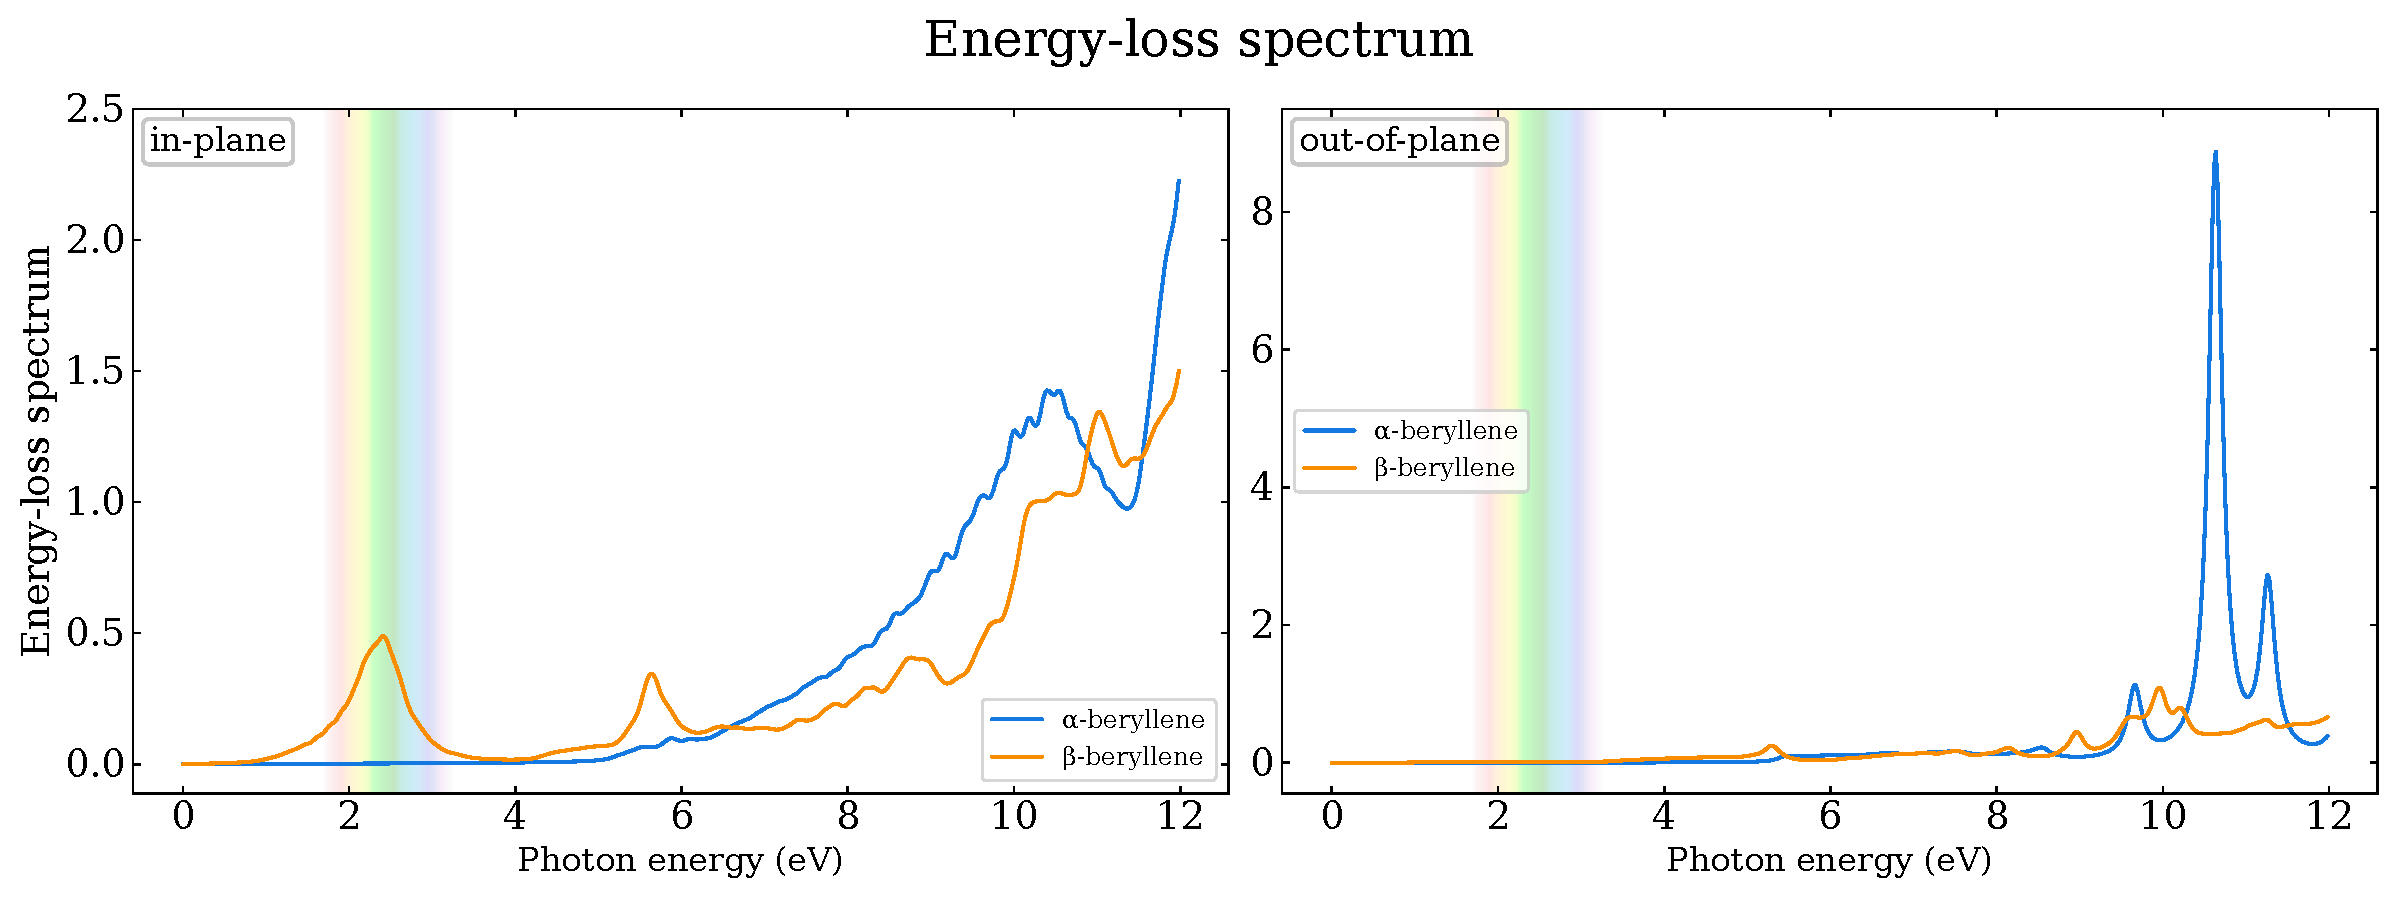
\includegraphics[width=0.80\linewidth]{figures_proj3/optics_alpha-beta_energy-loss_thesis.pdf}
\caption{Energy-loss spectrum for the in-plane and out-of-plane directions as a function of photon energy for $\alpha$-beryllene and $\beta$-beryllene.
The in-plane and out-of-plane curves correspond to the $xx$ and $zz$ components, respectively.}
\label{fig:proj3_energy_loss_alpha_beta}
\end{figure}

\begin{figure}[!htbp]
\centering
    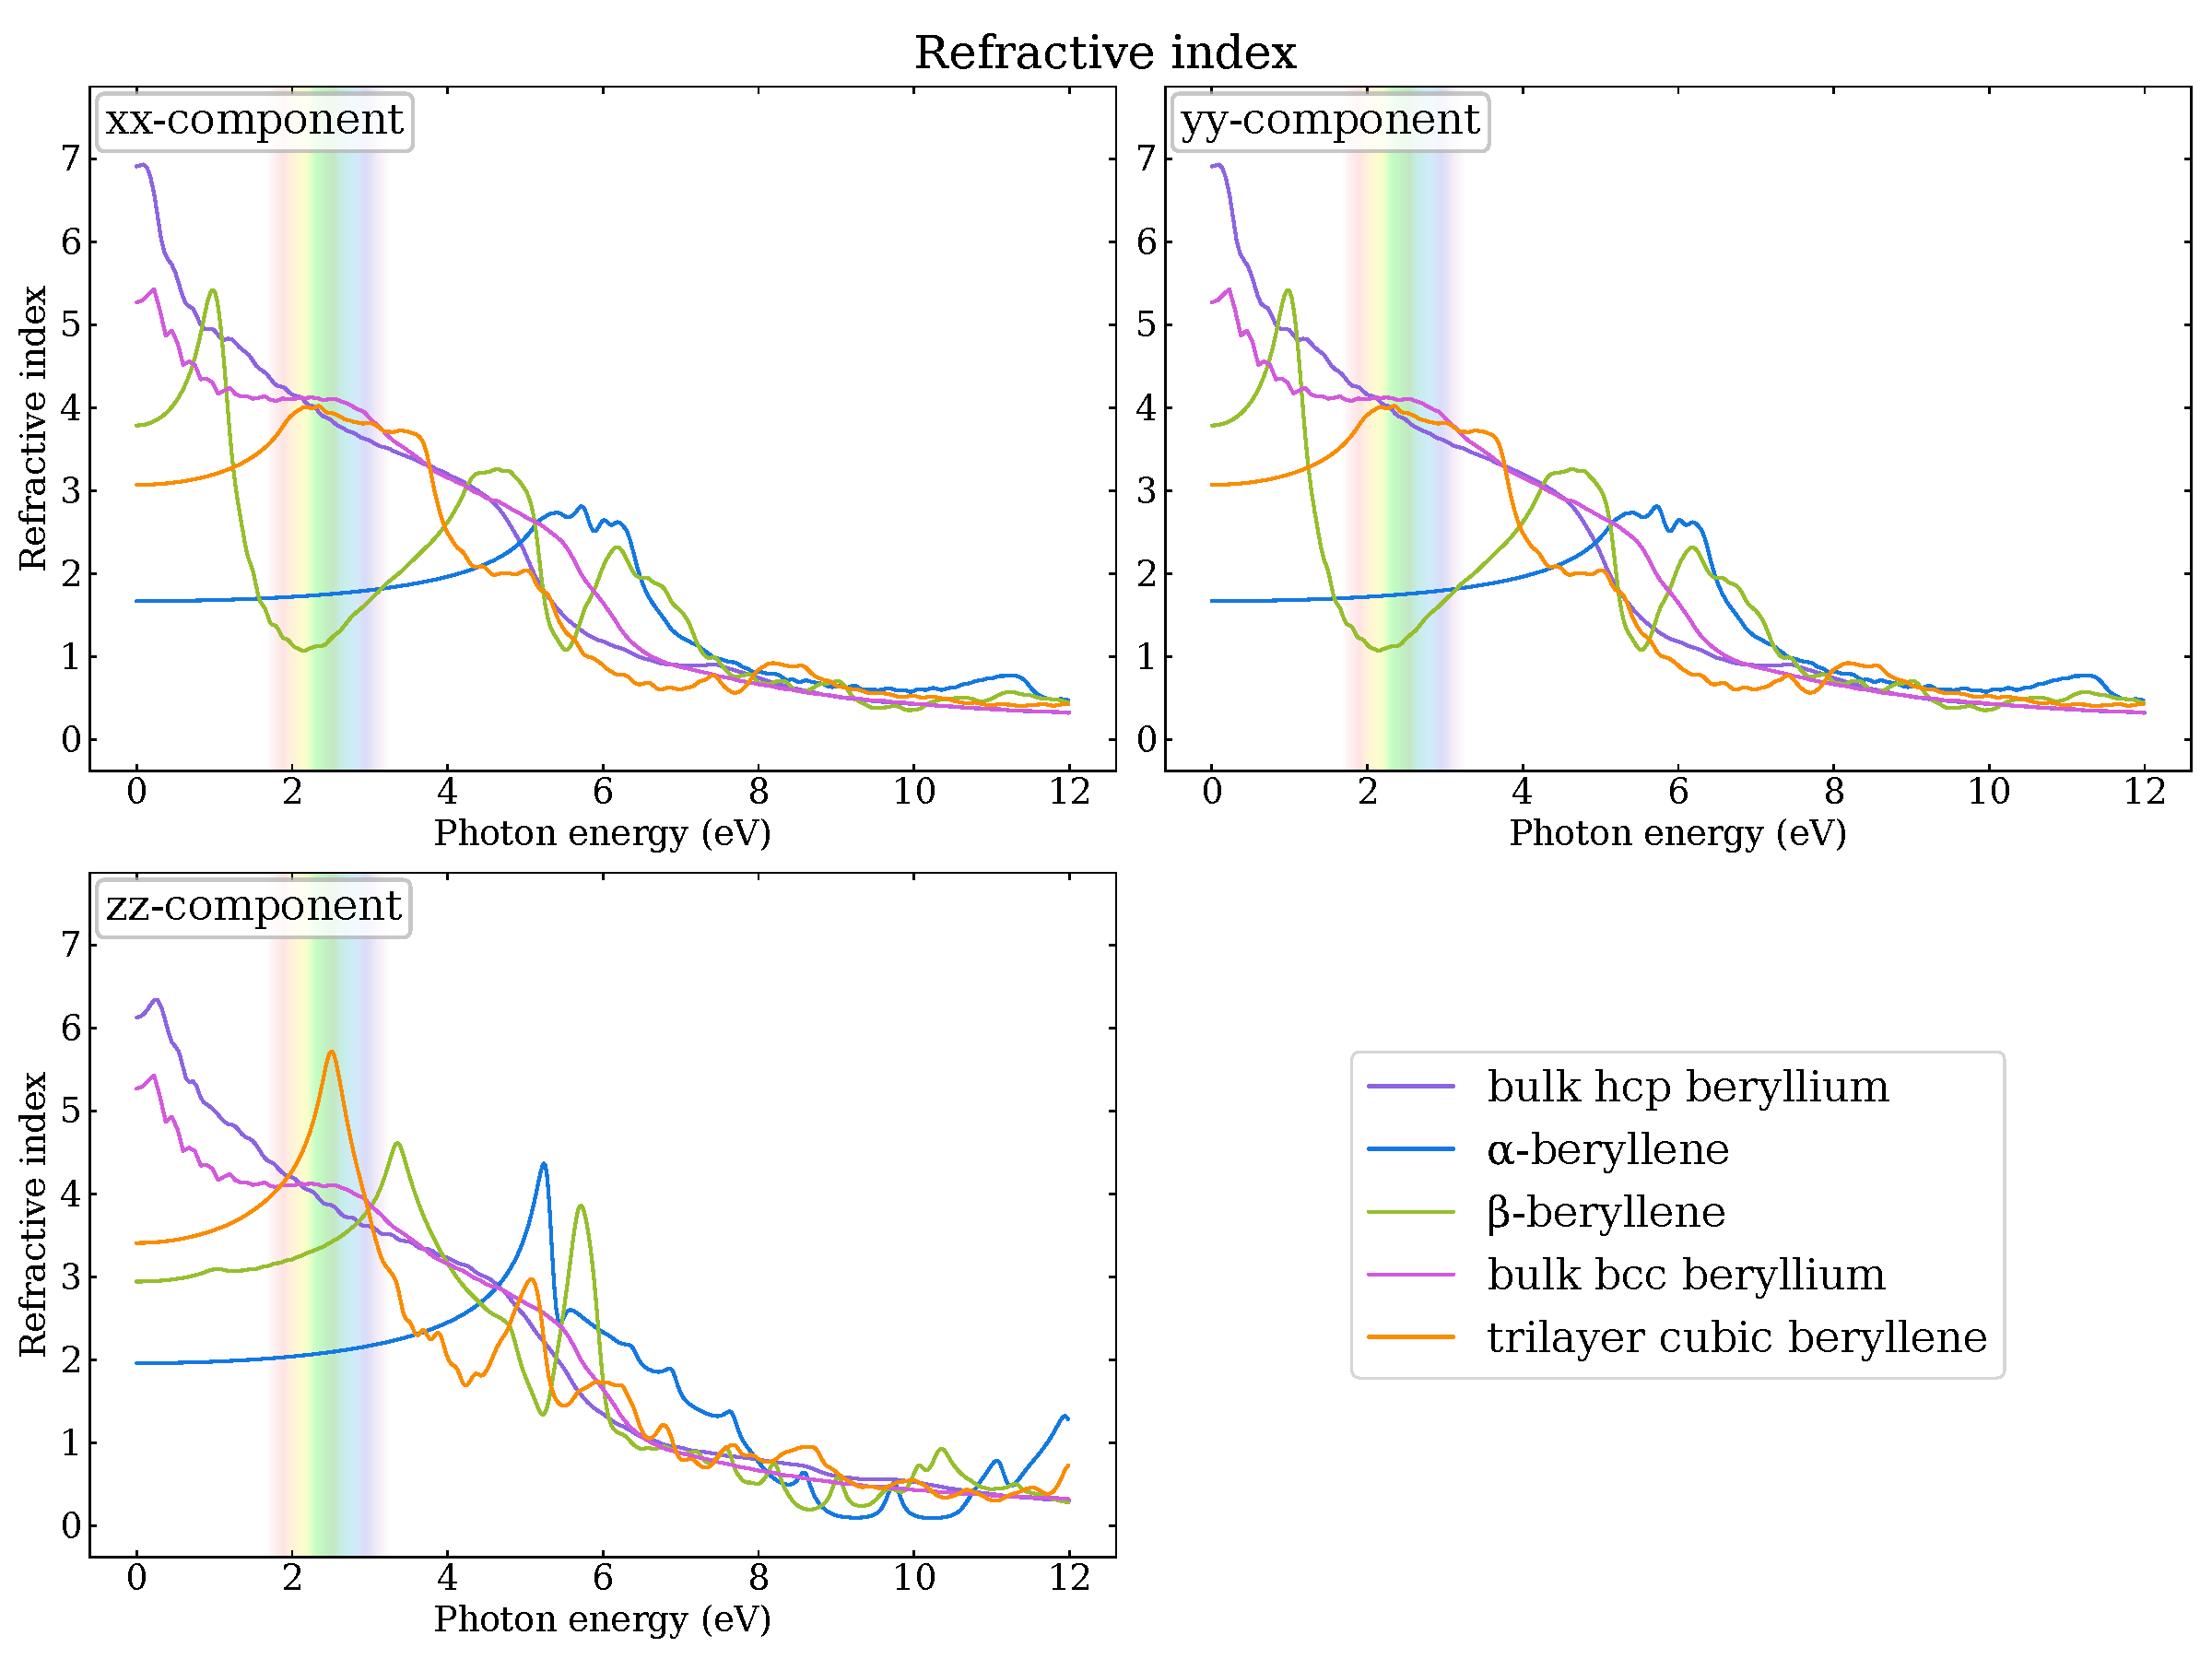
\includegraphics[width=0.80\linewidth]{figures_proj3/optics_pristine_refractive_thesis.pdf}
\caption{Refractive index for bulk hcp beryllium, $\alpha$-beryllene, $\beta$-beryllene,
bulk bcc beryllium, and trilayer cubic beryllene.
The spectra are shown for the $xx$,
$yy$,
and $zz$ components as functions of photon energy.}
\label{fig:proj3_optical_clean}
\end{figure}

\begin{figure}[!htbp]
\centering
    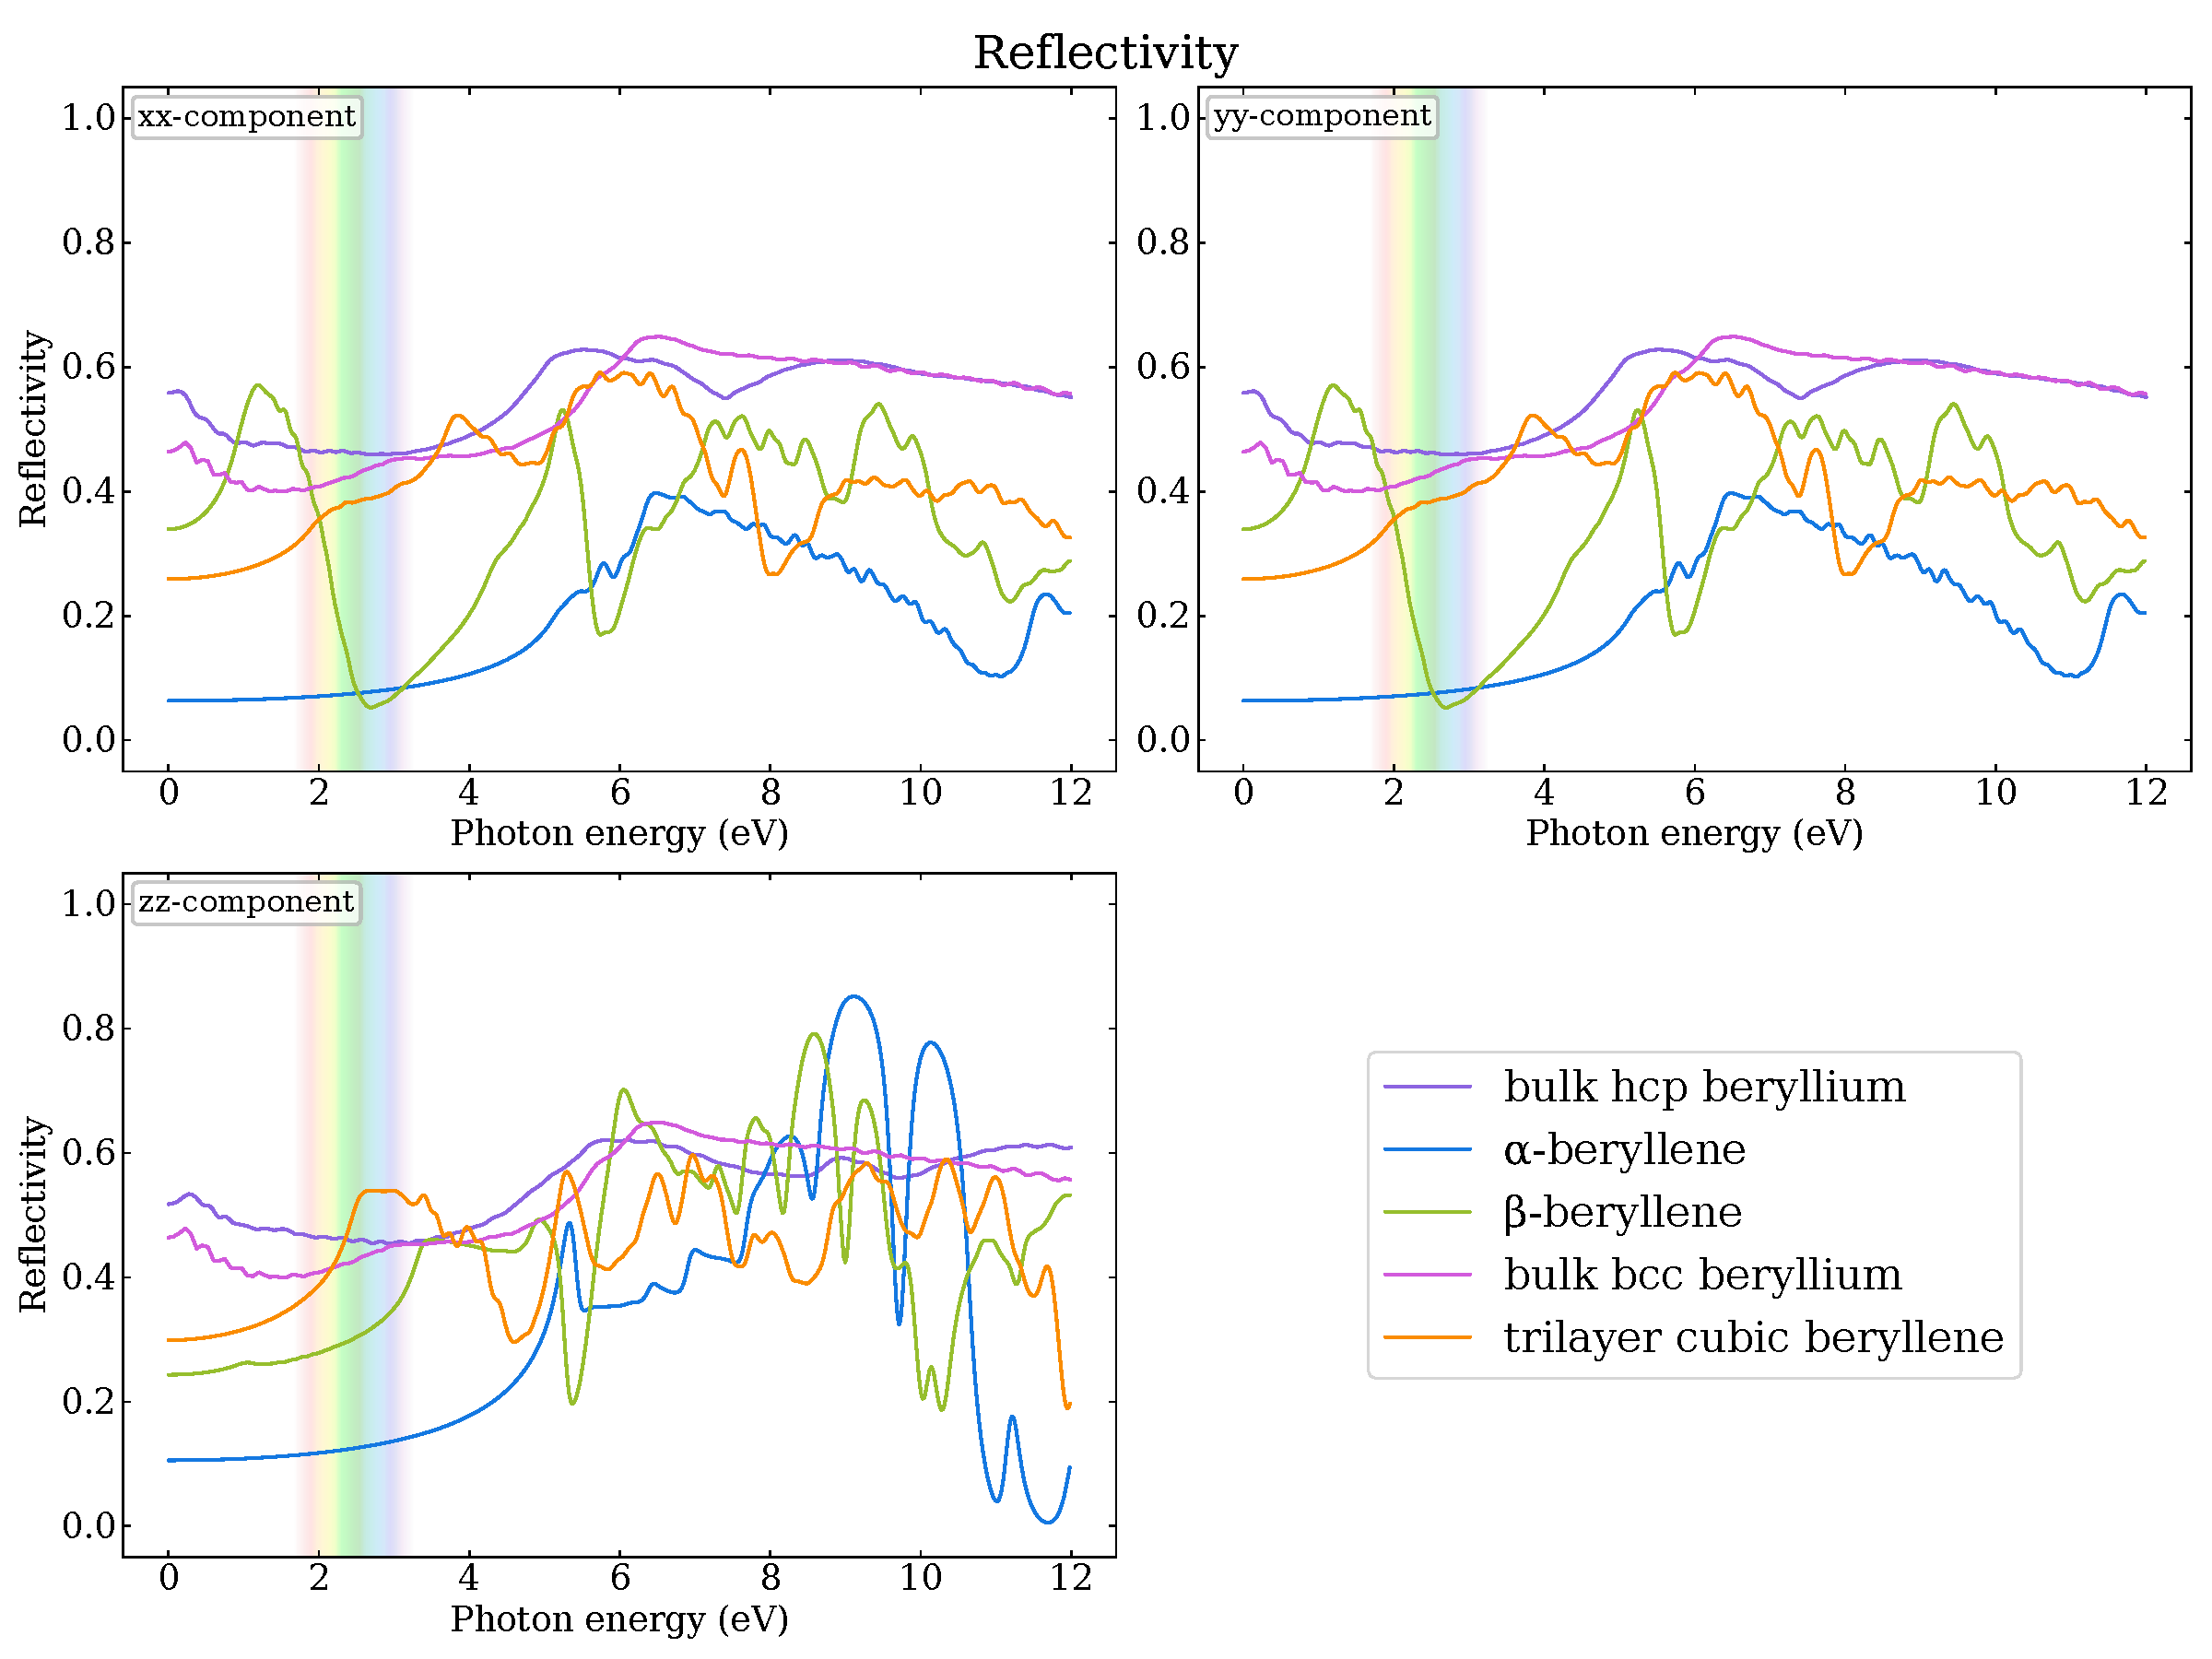
\includegraphics[width=0.80\linewidth]{figures_proj3/optics_pristine_reflectivity_thesis.pdf}
\caption{Reflectivity for bulk hcp beryllium, $\alpha$-beryllene, $\beta$-beryllene,
bulk bcc beryllium, and trilayer cubic beryllene.
The spectra are shown for the $xx$, $yy$,
and $zz$ components as functions of photon energy.}
\label{fig:proj3_optical_clean_reflectivity}
\end{figure}

\begin{figure}[!htbp]
\centering
    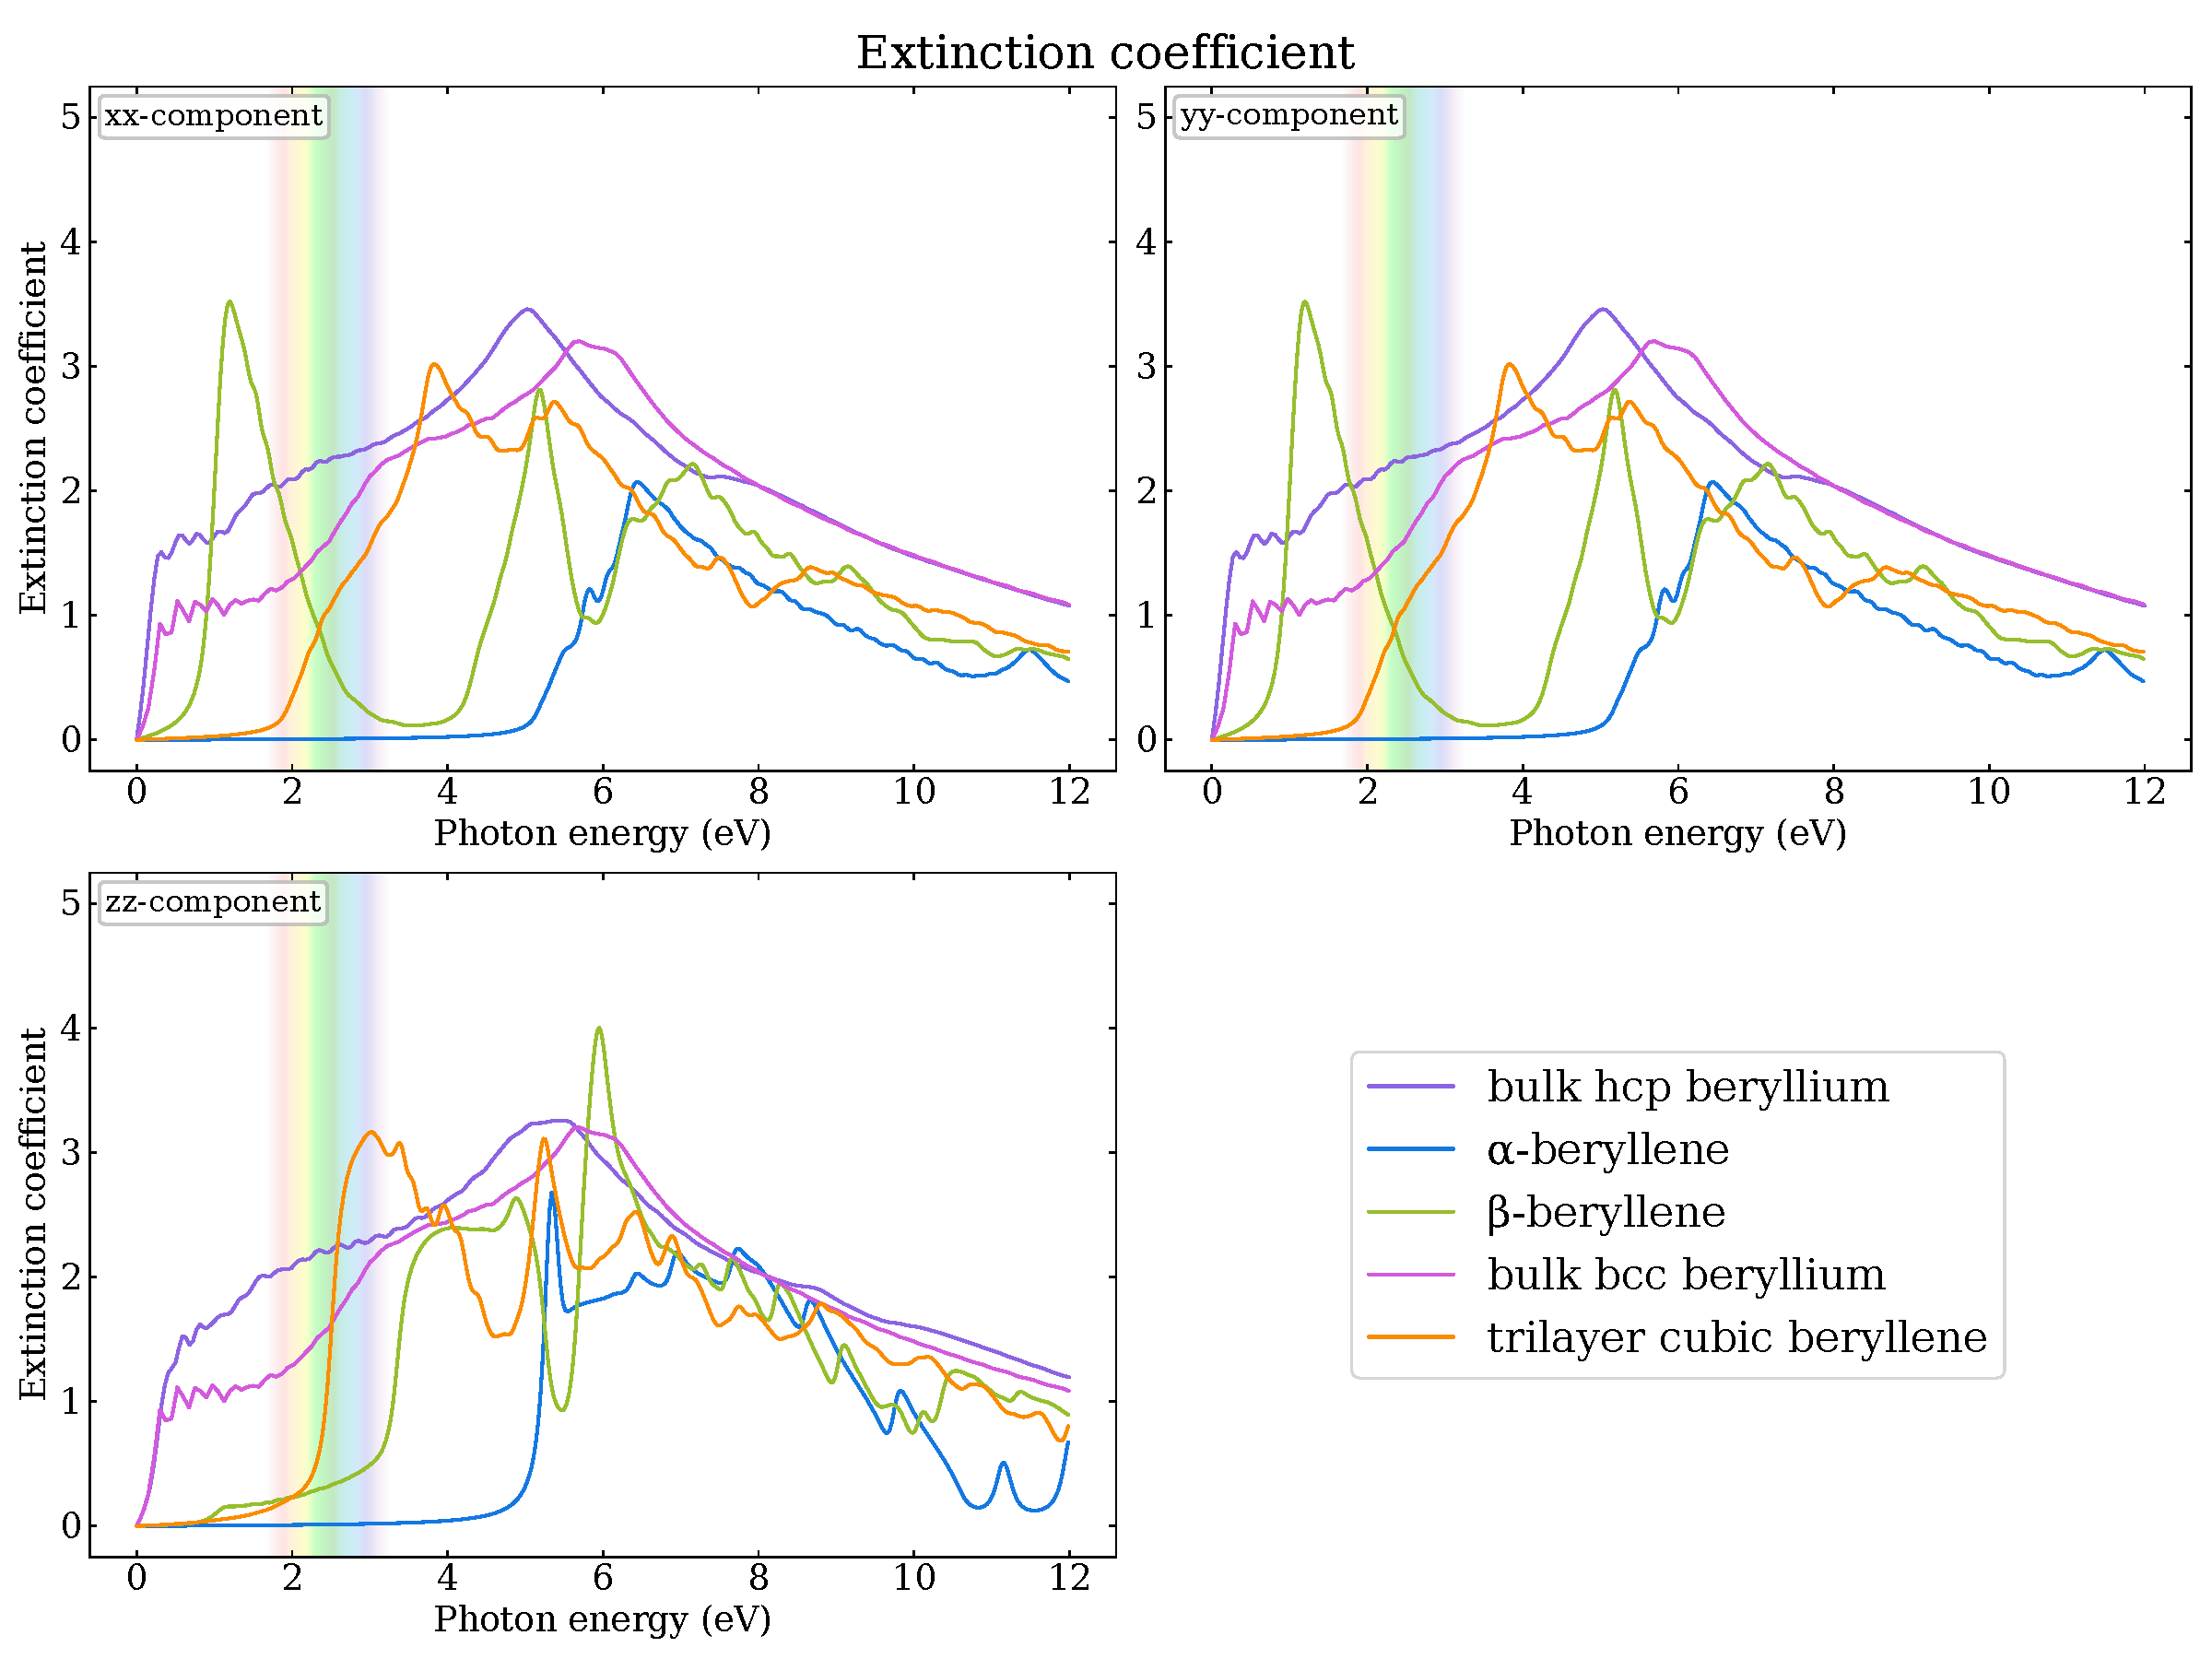
\includegraphics[width=0.80\linewidth]{figures_proj3/optics_pristine_extinction_thesis.pdf}
\caption{Extinction coefficient for bulk hcp beryllium, $\alpha$-beryllene, $\beta$-beryllene,
bulk bcc beryllium, and trilayer cubic beryllene.
The spectra are shown for the $xx$, $yy$,
and $zz$ components as functions of photon energy.}
\label{fig:proj3_optical_clean_extinction}
\end{figure}

\begin{figure}[!htbp]
\centering
    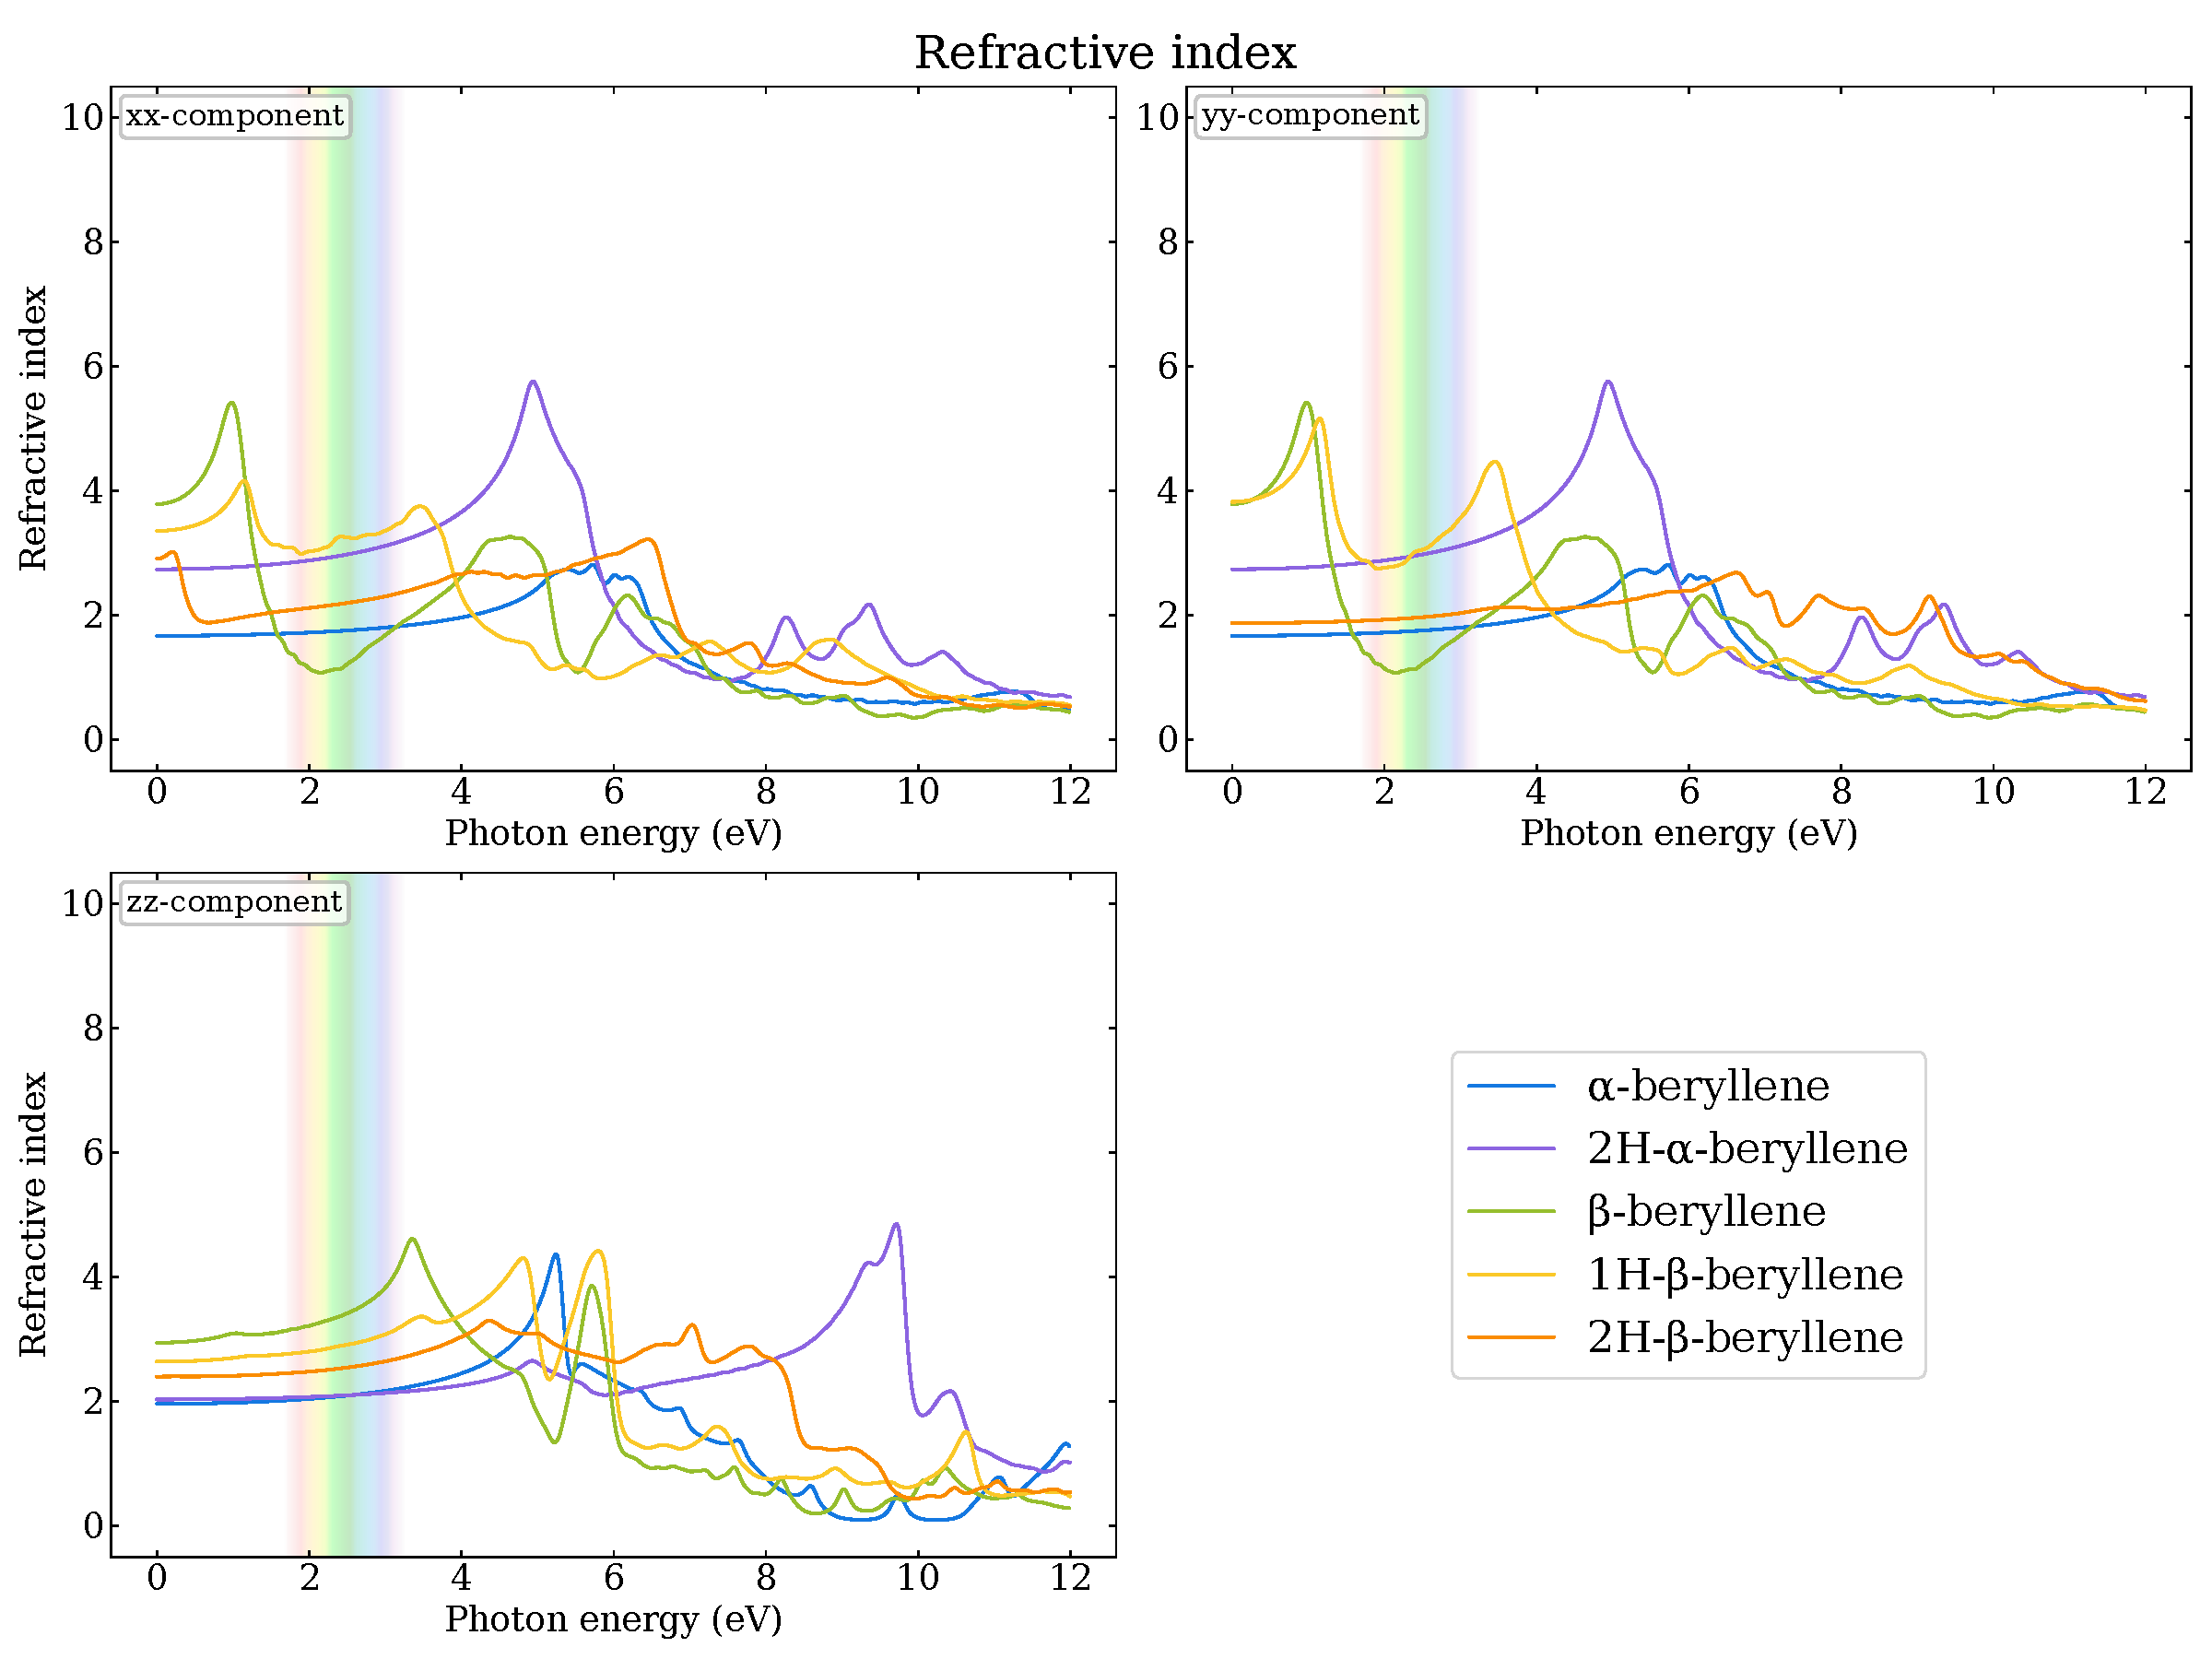
\includegraphics[width=0.80\linewidth]{figures_proj3/optics_hydrogenated_refractive_thesis.pdf}
\caption{Refractive index for pristine and hydrogen-functionalized $\alpha$-beryllene and $\beta$-beryllene structures.
The spectra are shown for the $xx$, $yy$,
and $zz$ components as functions of photon energy.}
\label{fig:proj3_optical_hydrogenated}
\end{figure}

\begin{figure}[!htbp]
\centering
    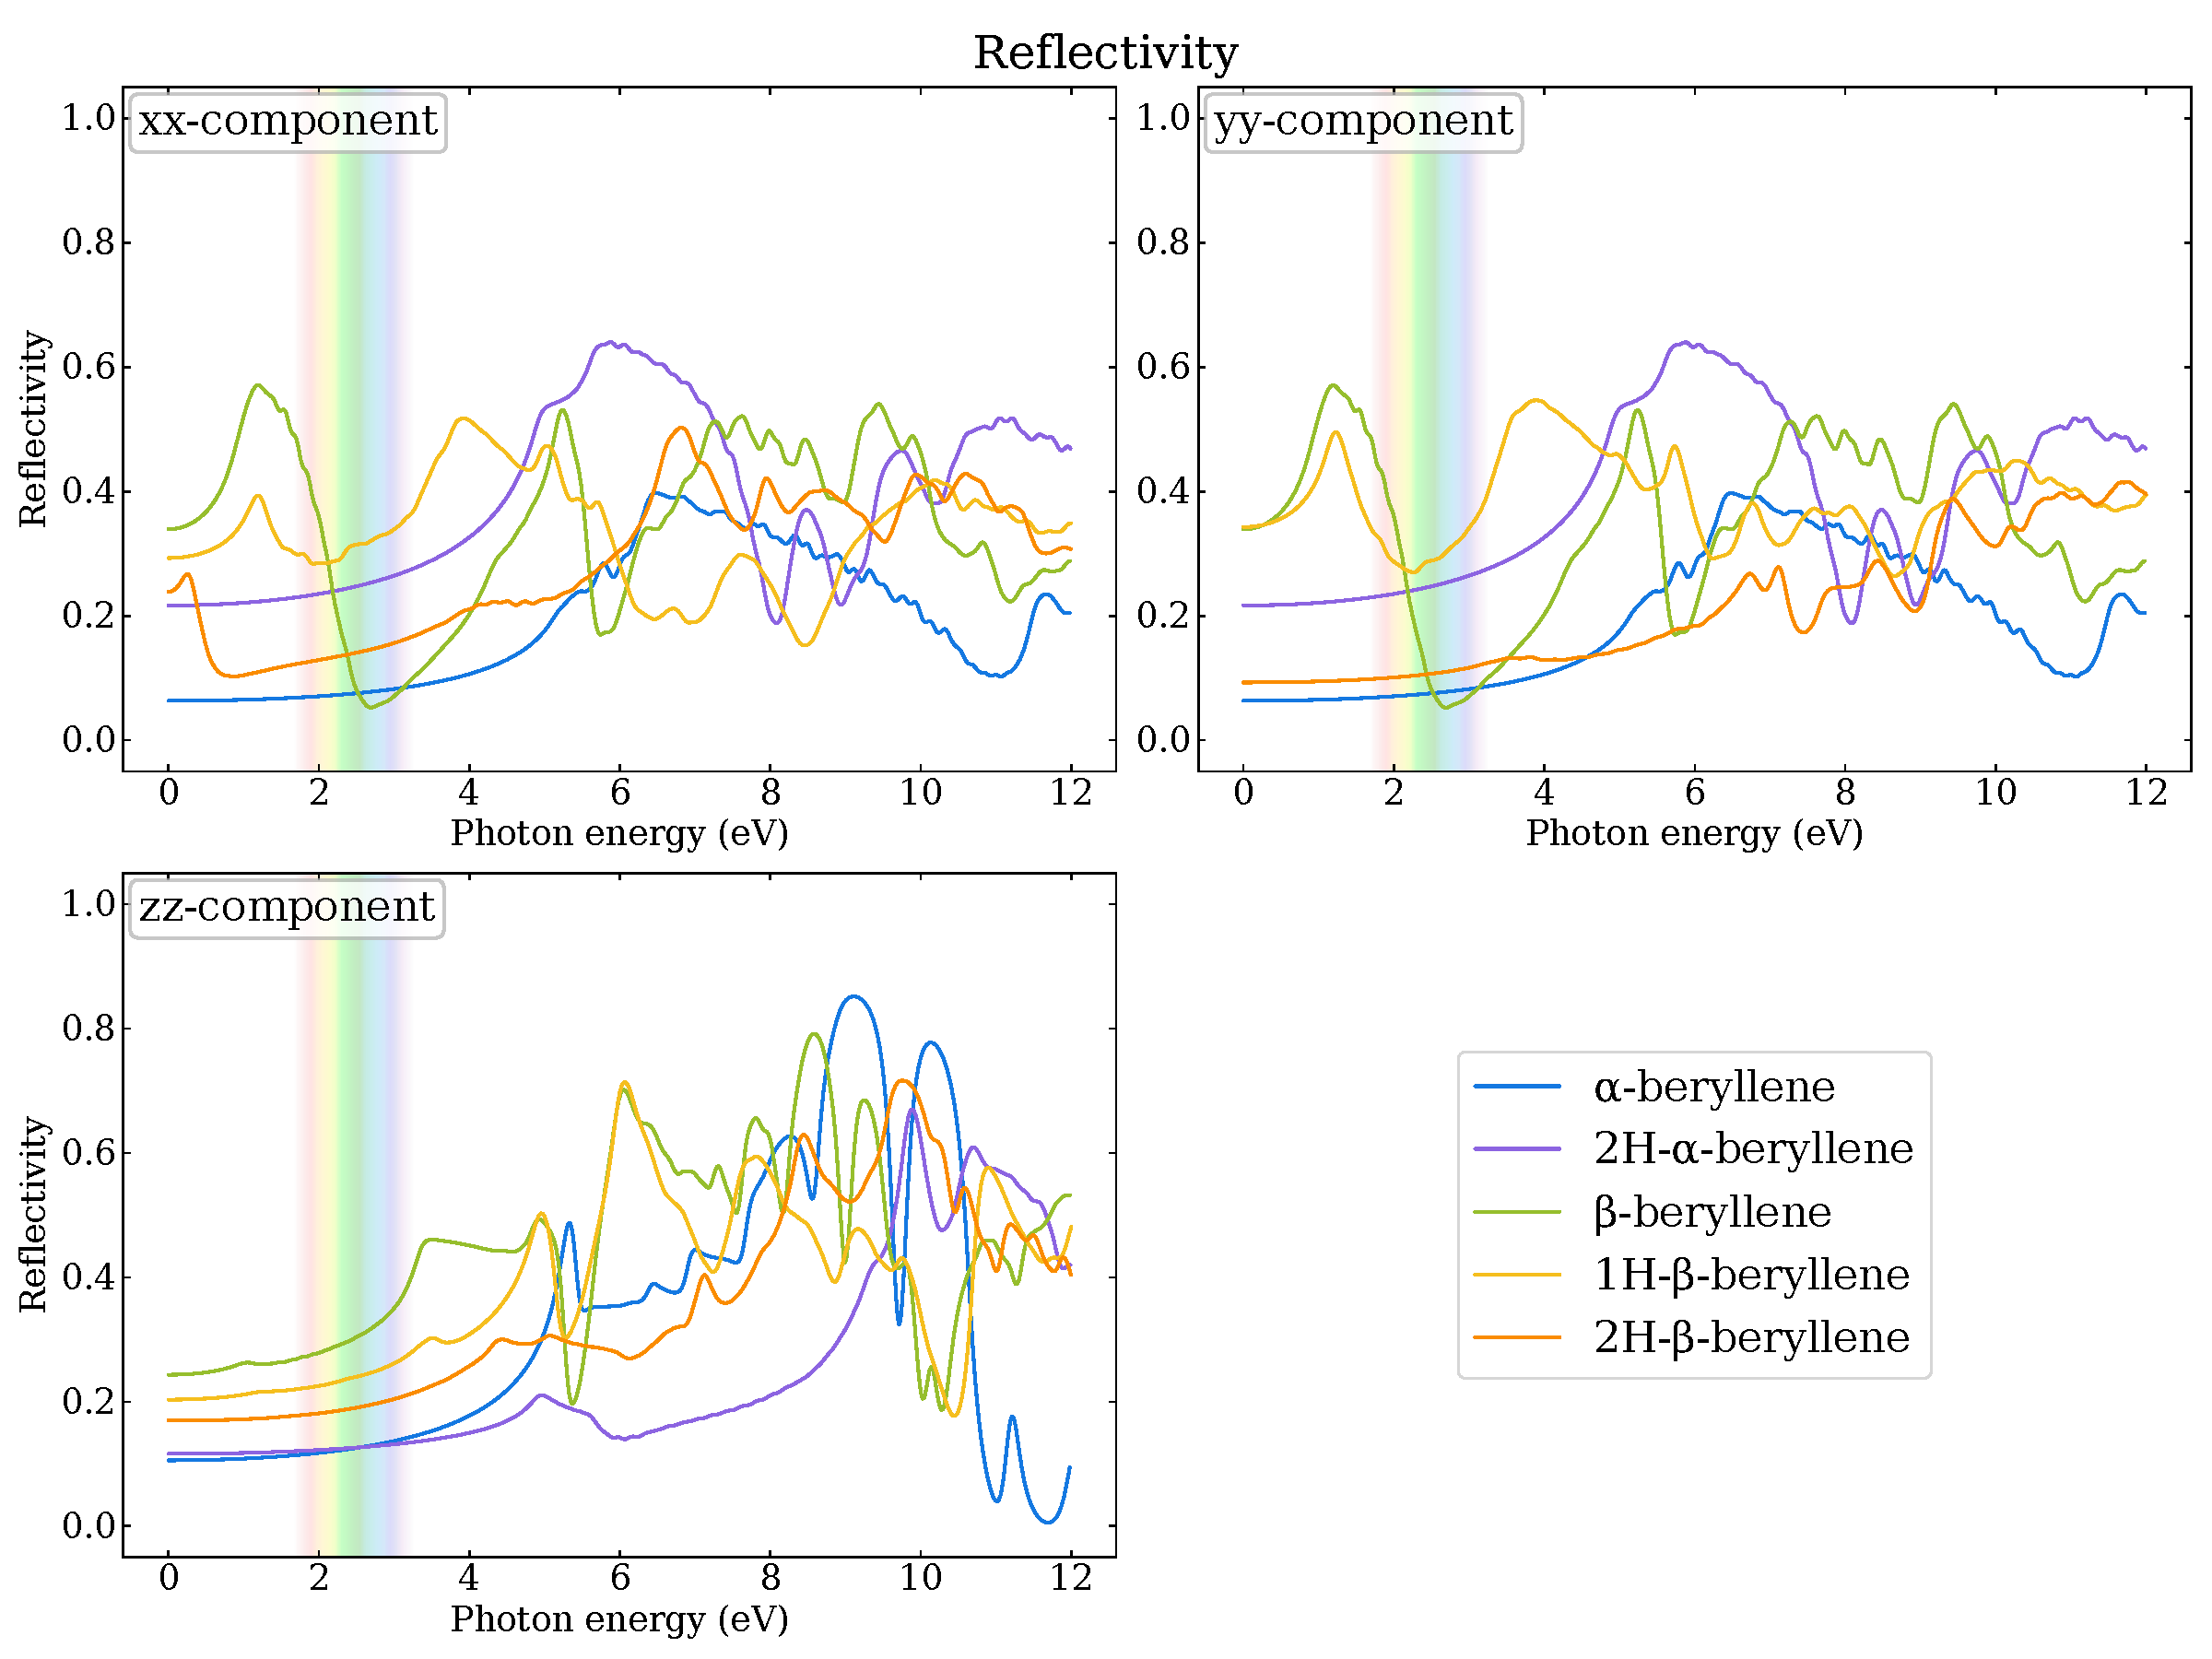
\includegraphics[width=0.80\linewidth]{figures_proj3/optics_hydrogenated_reflectivity_thesis.pdf}
\caption{Reflectivity for pristine and hydrogen-functionalized $\alpha$-beryllene and $\beta$-beryllene structures.
The spectra are shown for the $xx$, $yy$,
and $zz$ components as functions of photon energy.}
\label{fig:proj3_optical_hydrogenated_reflectivity}
\end{figure}

\begin{figure}[!htbp]
\centering
    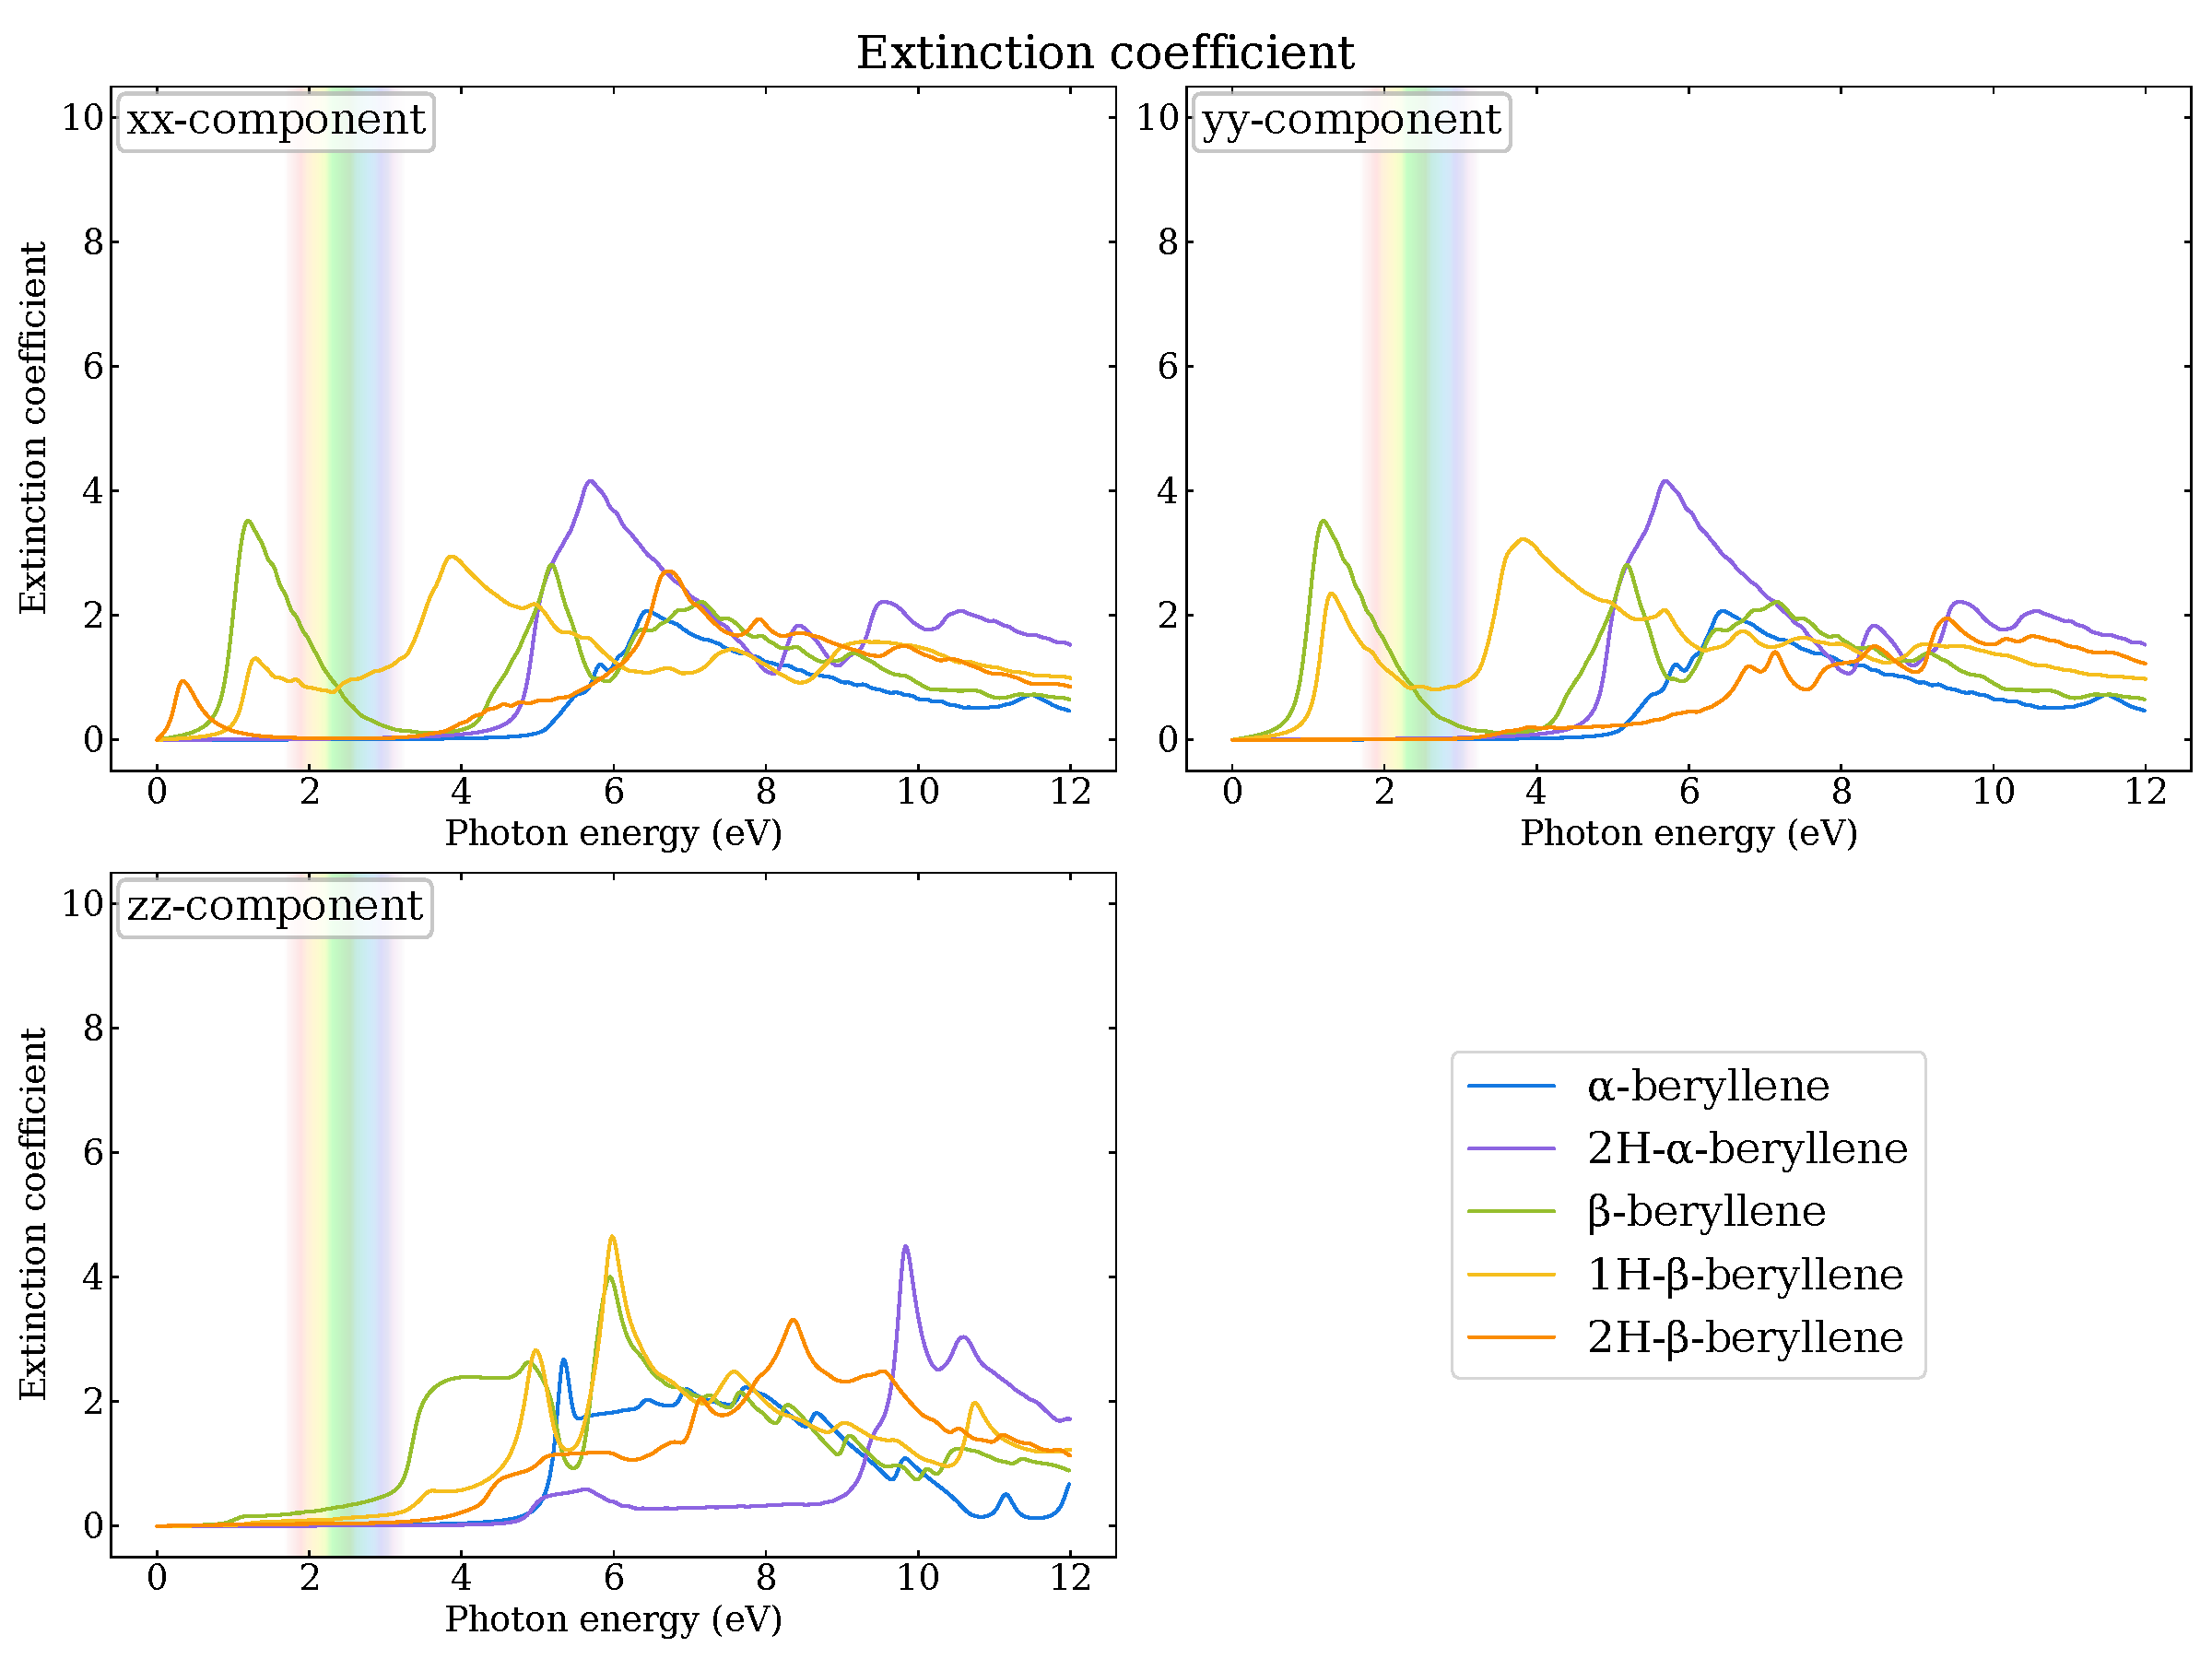
\includegraphics[width=0.80\linewidth]{figures_proj3/optics_hydrogenated_extinction_thesis.pdf}
\caption[Extinction coefficient for pristine and hydrogen-functionalized $\alpha$-beryllene and $\beta$-beryllene structures.
The spectra are shown for the $xx$, $yy$,
and $zz$ components as functions of photon energy.]{Extinction coefficient for pristine and\\
hydrogen-functionalized $\alpha$-beryllene and $\beta$-beryllene structures.
The spectra are shown for the $xx$, $yy$,
and $zz$ components as functions of photon energy.}
\label{fig:proj3_optical_hydrogenated_extinction}
\end{figure}

\cleardoublepage
\chapter{Conclusion and Outlook}
\label{cha:conclusion_outlook}
\setrunheadboth{Conclusion and Outlook}

We started this thesis with a question: how do changes in atomic structure modify the electronic structure and optical response of light-element two-dimensional materials?
To address this question, we compared graphene-based heterostructures, penta-bipyramid boron phases, and pristine and hydrogen-functionalized beryllene.
Each comparison begins with a specified structure and then changes its interface, dimensionality, or surface termination.
These changes redistribute charge, reorganize electronic states, and modify the response to an electromagnetic field.
For selected structures, we also examine how the electronic and lattice degrees of freedom enter magnetism, phonon-mediated pairing, and band topology.

We now collect the conclusions from these comparisons and examine how they connect to one another.
We then discuss the approximations that constrain their interpretation and the further calculations and experiments that can test them.
Throughout this discussion, we distinguish the properties of the calculated structures from the conditions needed to realize those structures experimentally.

\section{Conclusions from the material comparisons}
\label{sec:conclusions_material_comparisons}

We collect the main calculated quantities of the three comparisons in table~\ref{tab:conclusion_material_summary}.

\begin{table}[!htbp]
\centering
\rowcolors{2}{gray!15}{white}
\begin{adjustbox}{max width=1.0\linewidth,center}
\begin{tabular}{ccccccc}
\hline
\rowcolor{gray!25}
structure
& \begin{tabular}[c]{@{}c@{}}electronic\\nature\end{tabular}
& \begin{tabular}[c]{@{}c@{}}band gap\\(eV)\end{tabular}
& $\lambda$
& \begin{tabular}[c]{@{}c@{}}$T_\mathrm{c}^{\mathrm{AD}}$\\(K)\end{tabular}
& \begin{tabular}[c]{@{}c@{}}$T_\mathrm{c}^{\mathrm{aniso}}$\\(K)\end{tabular}
& $\mathbb{Z}_2$ \\
\hline
\rowcolor{white}
\multicolumn{7}{c}{chapter~\ref{cha:project_bilayers}: graphene-based heterostructures} \\
\hline
Graphene-Borophene & metallic & -- & -- & -- & -- & -- \\
Graphene-\ce{BC3} & semimetallic & -- & -- & -- & -- & -- \\
Graphene-\ce{B4C3} & semimetallic & -- & -- & -- & -- & -- \\
\hline
\rowcolor{white}
\multicolumn{7}{c}{chapter~\ref{cha:project_boron}: pentagonal-bipyramid boron phases} \\
\hline
bulk o-\ce{B14} & metallic & -- & 0.931 & 28.2 & $>30$ & -- \\
monolayer o-\ce{B14} & semiconductor & 0.105 & 0.05 & -- & -- & -- \\
bilayer o-\ce{B14} & semiconductor & 0.67 & -- & -- & -- & -- \\
\begin{tabular}[c]{@{}c@{}}hydrogen-terminated\\bilayer o-\ce{B14}\end{tabular} & metallic & -- & 1.01 & 18.5 & $\approx 26$ & -- \\
\hline
\rowcolor{white}
\multicolumn{7}{c}{chapter~\ref{cha:project_beryllene}: pristine and hydrogen-functionalized beryllene} \\
\hline
$\alpha$-beryllene & metallic & -- & -- & -- & -- & 1 \\
$\beta$-beryllene & metallic & -- & -- & -- & -- & 0 \\
trilayer cubic beryllene & metallic & -- & 0.46 & 2.0 & -- & 1 \\
2H-$\alpha$-beryllene & semiconductor & 6.00 & -- & -- & -- & 0 \\
1H-$\beta$-beryllene & metallic & -- & 0.61 & 8.1 & $\approx 14.2$ & 0 \\
2H-$\beta$-beryllene & metallic & -- & 1.40 & 21.9 & $\approx 31.7$ & 0 \\
\hline
\end{tabular}
\end{adjustbox}
\caption{Electronic nature, band gap, electron-phonon coupling strength $\lambda$,
Allen--Dynes transition temperature $T_\mathrm{c}^{\mathrm{AD}}$ for $\mu^*=0.13$,
anisotropic Migdal--Eliashberg transition temperature $T_\mathrm{c}^{\mathrm{aniso}}$,
and $\mathbb{Z}_2$ index of the main structures in the three research chapters.
The band gaps are HSE06 values.
The gap of monolayer o-\ce{B14} refers to its antiferromagnetic state, whereas its coupling strength refers to the non-magnetic PBE reference.
The pristine o-\ce{B14} bilayer is semimetallic with PBE.
For 2H-$\beta$-beryllene, the electron-phonon quantities refer to the structure relaxed with the D3 dispersion correction.
The $\mathbb{Z}_2$ indices refer to the selected band subspaces and are conditional for the metallic structures.}
\label{tab:conclusion_material_summary}
\end{table}

\subsection{Interfacial coupling in graphene-based heterostructures}

Firstly, chapter~\ref{cha:project_bilayers} examines how an adjacent boron-containing layer modifies graphene.
The constituent monolayers already span different electronic characters: graphene is a semimetal, borophene is metallic, and the selected \ce{BC3} and \ce{B4C3} monolayers are indirect-gap semiconductors.
HSE06 gives gaps of \qty{1.822}{\electronvolt} and \qty{2.381}{\electronvolt} for the latter two monolayers, respectively.
Stacking these constituents therefore compares the effect of coupling graphene to either a metallic layer or a semiconducting layer within the same study.

The resulting Graphene-Borophene heterostructure remains metallic, whereas Graphene-\ce{BC3} and Graphene-\ce{B4C3} display semimetallic band structures.
The graphene-derived bands remain recognizable near the $\mathrm{K}$ point.
Interlayer coupling opens local gaps of approximately \qty{50}{\milli\electronvolt} in Graphene-\ce{BC3} and \qty{20}{\milli\electronvolt} in Graphene-\ce{B4C3} at this point, while both bilayers remain semimetallic.
The charge-density differences further show interfacial redistribution from graphene towards the boron-containing layer, with the largest redistribution in the studied Graphene-\ce{BC3} structure.
The local atomic arrangement therefore modifies the coupling even when the layers retain recognizable features of their isolated electronic structures.

The band alignment gives another view of the interface.
Within the Schottky--Mott comparison, the graphene contact favours an n-type alignment with \ce{BC3} and a p-type alignment with \ce{B4C3}.
The opposite alignment tendencies show that changing the boron-carbide constituent changes the relative position of the graphene Fermi level and the semiconductor band edges.
They identify which carrier barrier is smaller within this alignment model.
The contact geometry and carrier transmission then determine the injection current.

The optical spectra resolve further differences between the heterostructures.
All three absorb within the visible region in the calculated response, while the relative strengths depend on photon energy and polarization.
Graphene-Borophene has the stronger absorption near the low-energy rise around \qty{1}{\electronvolt}.
The sub-\unit{\electronvolt} in-plane energy-loss peaks occur in the two graphene--boron-carbide heterostructures and are absent from the corresponding Graphene-Borophene spectra.
We therefore need to compare absorption and energy loss separately, since the two quantities probe different aspects of the dielectric response.

We therefore arrive at an interface whose constituent layers remain electronically recognizable, but whose alignment and response depend on their interaction.
Retaining the graphene-derived dispersion does not leave the optical spectrum unchanged: the adjacent layer contributes its own states, and the combined system develops a different distribution of transition energies and strengths.
The comparison with the isolated monolayers identifies these changes and connects them to the formation of the interface.

\subsection{Dimensional reduction and termination in the boron framework}

Next, chapter~\ref{cha:project_boron} follows the pentagonal-bipyramid framework from bulk o-\ce{B14} to monolayer and bilayer structures, and then to hydrogen-terminated sheets.
Here, reducing the number of layers changes the coordination within the boron network itself.
Hydrogen termination subsequently changes the bonding at its exposed surfaces.
The resulting electronic structures show that these two operations produce different trends.

Among the tested magnetic configurations, the HSE06 calculation favours the antiferromagnetic monolayer over the ferromagnetic monolayer and gives a gap of \qty{0.105}{\electronvolt}.
The spin density locates the magnetic moments mainly on the apical boron atoms of the bipyramids.
This spatial information connects the magnetic state to particular sites within the reduced framework.
The pristine bilayer has a different character: HSE06 opens a gap of \qty{0.67}{\electronvolt}, whereas PBE gives a semimetallic result.
Hydrogen termination then produces a metallic bilayer.
Therefore, the effect of hydrogen in this structural family depends on the electronic states and bonding of the starting sheet.

The electron-phonon calculations predict appreciable phonon-mediated pairing in bulk o-\ce{B14} and the hydrogen-terminated bilayer.
For a Coulomb pseudopotential $\mu^*=0.13$, the Allen--Dynes estimates give transition temperatures of \qty{28.2}{\kelvin} and \qty{18.5}{\kelvin}, respectively.
The hydrogen-terminated bilayer has the larger coupling strength, $\lambda=1.01$, compared with $\lambda=0.931$ in the bulk, but it has the lower estimated transition temperature.
This comparison illustrates that $T_{\mathrm{c}}$ depends on more than the coupling strength.
The phonon frequencies entering the pairing problem also control its energy scale~\cite{allen-dynes}.
The anisotropic calculations further resolve a distribution of superconducting gaps that shifts towards lower energies as temperature increases.
These distributions place $T_{\mathrm{c}}$ above \qty{30}{\kelvin} for the bulk and close to \qty{26}{\kelvin} for the hydrogen-terminated bilayer.

The stability results constrain this interpretation.
The hydrogen-terminated monolayer develops a clear harmonic instability, while the terminated bilayer retains small imaginary frequencies near $\Gamma$.
The terminated bilayer retains its bonding framework during the reported \qty{400}{\kelvin} molecular-dynamics trajectory, leaving the long-wavelength question open.
The superconducting prediction therefore concerns the specified bilayer structure and its calculated electronic and vibrational reference.

The optical calculations reveal strong directional differences across the boron structures.
They use a non-spin-polarized PBE reference, including for the monolayer.
Consequently, these spectra characterize that reference, and the HSE06 antiferromagnetic semiconductor requires a further calculation.
Within this reference, the largest absorption coefficients in the visible interval occur for the pristine bilayer in the $xx$ component, the hydrogen-terminated bilayer in $yy$, and the bulk in $zz$.
The different directional comparisons therefore select different structures.
Together with the electronic and electron-phonon results, this finding shows how the same boron framework accommodates different responses as its coordination and termination change.

\subsection{Structure, hydrogenation, band topology, and superconductivity in beryllene}

Finally, chapter~\ref{cha:project_beryllene} examines the $\alpha$ and $\beta$ phases of beryllene, extends the comparison to an ABA-stacked square-lattice trilayer, and investigates selected hydrogen arrangements.
The retained hydrogen-functionalized structures are 2H-$\alpha$-, 1H-$\beta$-, and 2H-$\beta$-beryllene.
This comparison separates changes in the beryllium framework from changes in hydrogen coverage and arrangement.
The analysis follows the stability question from small lattice displacements to hydrogen exchange with the environment and competition with another geometry.

Pristine $\alpha$-beryllene, $\beta$-beryllene, and trilayer cubic beryllene have no imaginary phonon frequencies in the reported harmonic calculations.
Their cohesive energies nevertheless remain less favourable than that of bulk hcp beryllium.
They therefore represent candidate two-dimensional structures.
Among the hydrogen-functionalized structures, 2H-$\alpha$-beryllene also satisfies the reported harmonic stability test.
For 1H-$\beta$-beryllene, the long-wavelength flexural behaviour remains unresolved, as the sampled commensurate modes are real, but the interpolated branch develops imaginary frequencies near $\Gamma$.
2H-$\beta$-beryllene has a soft mode at a commensurate wave vector, so this instability appears in the directly calculated frequencies.

The frozen-phonon calculation resolves a shallow double well along this mode of 2H-$\beta$-beryllene, with a depth of at most \qty{0.2}{\milli\electronvolt} in the 20-atom supercell.
The one-mode quantum ground state lies approximately \qty{6}{\milli\electronvolt} above the well bottom and remains centred at the undistorted structure.
In this model, the comparison of these energy scales shows that quantum motion extends across the shallow wells, beyond the classical minimum.
This result supports suppression of a static distortion along the selected coordinate.
The hydrogen-functionalized structures also retain their frameworks during \qty{5.5}{\pico\second} trajectories at \qty{300}{\kelvin}, establishing their persistence over the simulated interval.

The hydrogen free energies refine the comparison further.
At \qty{298.15}{\kelvin} and a hydrogen pressure of \qty{1}{\bar},
the adsorption free energies are \qty{-0.08}{\electronvolt},
\qty[retain-explicit-plus]{+0.17}{\electronvolt}, and \qty[retain-explicit-plus]{+0.06}{\electronvolt} per hydrogen atom for 2H-$\alpha$-, 1H-$\beta$-, and 2H-$\beta$-beryllene, respectively.
The reference in each case consists of the corresponding pristine sheet and molecular hydrogen.
Thus, only 2H-$\alpha$-beryllene favours adsorption under these conditions.
Formation from bulk beryllium is a separate comparison.
Moreover, a relaxed puckered square-layer \ce{BeH2} candidate lies \qty{38}{\milli\electronvolt} per formula unit below 2H-$\alpha$-beryllene in electronic energy.
Its phonon stability and the reconstruction barrier remain uncalculated.
The result identifies a competing geometry and leaves the kinetic persistence of the triangular sheet as a separate question.

Hydrogen changes the electronic character differently in the two beryllene families.
The pristine structures and the hydrogen-functionalized $\beta$-beryllene structures remain metallic.
In contrast, 2H-$\alpha$-beryllene develops an indirect gap of \qty{4.84}{\electronvolt} with PBE and \qty{6.00}{\electronvolt} with HSE06.
The same operation, hydrogen addition, therefore produces a wide-gap semiconductor in one framework and retains metallic bands in another.
This difference reinforces the need to follow the actual bonding geometry.

The topological analysis concerns selected band subspaces.
The reported spin-orbit-coupled calculations give non-trivial $\mathbb{Z}_2$ indices for the lowest two spinor bands of $\alpha$-beryllene and the lowest six spinor bands of trilayer cubic beryllene.
These indices are conditional on the isolation of the two subspaces throughout the Brillouin zone.
The minimum sampled direct gaps are only \qty{1.13}{\milli\electronvolt} and \qty{0.735}{\milli\electronvolt}, respectively.
The relevant gaps lie above the Fermi level, and both neutral structures remain metallic.
These results therefore identify conditional non-trivial subspaces in structures that remain metallic at neutral filling.
The selected subspaces of $\beta$-beryllene and the hydrogen-functionalized structures give trivial indices, and for metallic systems these fixed subspaces again differ from an occupied insulating manifold.
The indices of $\alpha$- and $\beta$-beryllene agree with the earlier classification~\cite{li2023coexistence}.

In addition to the earlier predictions for $\alpha$- and $\beta$-beryllene~\cite{li2023coexistence}, the electron-phonon calculations predict phonon-mediated superconductivity in trilayer cubic beryllene, 1H-$\beta$-beryllene, and 2H-$\beta$-beryllene.
Trilayer cubic beryllene has the weakest coupling, $\lambda=0.46$, and an isotropic Migdal--Eliashberg transition temperature of \qty{3.7}{\kelvin}.
2H-$\beta$-beryllene has the strongest coupling, $\lambda=1.40$, and the anisotropic Migdal--Eliashberg solution places its $T_{\mathrm{c}}$ at approximately \qty{31.7}{\kelvin}.
The electron-phonon calculations of 2H-$\beta$-beryllene use a structure relaxed with the D3 dispersion correction, in which the soft mode is absent.
For 1H-$\beta$-beryllene, the gap anisotropy raises $T_{\mathrm{c}}$ from \qty{11.6}{\kelvin} to approximately \qty{14.2}{\kelvin}.

The optical response resolves changes beyond the metallic or semiconducting classification.
Trilayer cubic beryllene has weaker in-plane absorption than bulk bcc beryllium throughout the sampled visible interval, while its out-of-plane absorption exceeds the bulk value over only part of that interval.
Here, bulk bcc beryllium serves as a structural reference.
Its harmonic instability at zero pressure precludes treating it as a stable bulk counterpart under those conditions.
Hydrogenation likewise redistributes spectral strength without enhancing every component.
For 2H-$\alpha$-beryllene, the response below the main absorption region is weak and broadened, consistent with its wide electronic gap.
The beryllene comparison therefore yields several distinct outcomes.
They include the harmonically stable trilayer cubic beryllene, the wide-gap 2H-$\alpha$-beryllene, conditional non-trivial subspaces in two metallic parent structures, and phonon-mediated superconductivity in three metallic structures.
Their different stability and occupation conditions determine the role of each outcome in further work.

\section{Connections between the three studies}
\label{sec:conclusions_connections}

The preceding comparisons answer the common question from three directions.
An interface changes the environment of an existing layer, dimensional reduction changes atomic coordination, and hydrogen termination changes the surface bonding and electron count.
The calculated properties respond to these particular changes.
We now examine what the comparisons establish together.

Firstly, we can follow the structural changes through the charge distributions and orbital contributions.
In the graphene heterostructures, the relative positions of the two layers determine where charge accumulates and where it depletes.
Graphene-\ce{BC3} shows the largest redistribution among the three interfaces, consistent with its smaller interlayer separation and hollow-site coordination.
Hydrogen adsorption on the o-\ce{B14} bilayer also changes charge beyond the adsorption site: the calculated density increases in the interlayer B-B bonds and in the apical boron $p_z$ region directed towards hydrogen.
The corresponding interlayer bond becomes slightly shorter.
In hydrogen-functionalized beryllene, the projected densities of states resolve the mixing of hydrogen $1s$ states with beryllium $s$ and $p$ states.
Surface modification therefore reorganizes bonding within the layer as well as introducing new bonds at its surface.
The charge distributions and orbital contributions connect this rearrangement of atoms to the electronic response.

Next, the geometry of the bonding matters when we compare different layer numbers.
The graphene heterostructures couple two distinct sheets through an interface, whereas the o-\ce{B14} structures retain parts of a connected boron framework as we reduce its thickness.
The beryllene comparison introduces another change.
Trilayer cubic beryllene has a square lattice, while pristine $\alpha$- and $\beta$-beryllene belong to the hexagonal family.
Their differences therefore include lattice geometry as well as layer number.
Hydrogen adsorption further distorts the $\beta$-beryllene lattice and changes its symmetry.
1H-$\beta$-beryllene loses inversion symmetry, whereas 2H-$\beta$-beryllene retains it.
This distinction changes the available route to the $\mathbb{Z}_2$ index.
For 1H-$\beta$-beryllene, where the inversion-based parity criterion no longer applies, we use Wilson loops.
Layer number and composition identify a structure only partially.
The atomic arrangement specifies the bonding and symmetry needed to interpret its properties.

These microscopic comparisons account for the different electronic trends with thickness and hydrogen coverage.
The HSE06 semiconducting o-\ce{B14} bilayer becomes metallic after termination, whereas metallic $\alpha$-beryllene becomes a wide-gap semiconductor.
Hydrogen introduces orbitals and changes bonding in both cases, but the starting states and the resulting networks differ.
The comparison therefore concerns a reorganization of the electronic structure, whose outcome depends on the parent material and adsorption geometry.

Once we inspect the resulting bands, we also distinguish their local separations from the electronic character of the complete system.
The small gaps near the graphene-derived $\mathrm{K}$ point coexist with semimetallic bilayer bands elsewhere.
In beryllene, direct isolation of a selected subspace can likewise coexist with a metallic Fermi level.
The former separation identifies a local change in dispersion, whereas the latter defines the subspace whose topology we can classify.
An insulating bulk additionally requires the occupied and empty states to remain separated at the actual filling.
The same band structure can therefore support several different conclusions, depending on whether we ask about a local crossing, the geometry of a subspace, or charge transport.

The optical comparisons carry this reasoning beyond the band energies.
The dielectric response depends on the available transitions and their polarization-dependent matrix elements, so the optical spectrum contains more than the distinction between a metal and a semiconductor.
The calculated in-plane and out-of-plane responses separate even within one structure.
Changing the structure can strengthen one spectral region while weakening another.
Therefore, the appropriate comparison specifies the direction, photon-energy interval, and response quantity before discussing an enhancement.
This conclusion connects the material calculations to the linear-response formulation in chapter~\ref{cha:fundamentals_b}.

Finally, a consistent conclusion requires the structural and electronic descriptions to refer to the same physical state.
An optical spectrum of a non-magnetic reference describes that reference, separate from the gap of an antiferromagnetic calculation.
A superconducting estimate for a proposed sheet presupposes that the sheet and its vibrational reference remain meaningful.
A $\mathbb{Z}_2$ index requires the selected subspace to retain the symmetry and isolation assumed in its calculation.
We therefore arrive at a common procedure: establish the structural and electronic reference, determine the response within that reference, and then examine whether the conditions survive the next level of description.
This procedure connects the three projects while preserving the physical differences between them.

\section{Limitations of the present work}
\label{sec:conclusions_limitations}

The calculations establish comparisons within specified approximations.
We now examine where these approximations constrain the conclusions.
The main limitations concern the electronic reference, the treatment of optical excitations, the stability of the proposed structures, and the small energy scales of selected quantum properties.

The exchange-correlation approximation affects both quantitative gaps and, in some cases, the electronic classification.
The PBE and HSE06 results for the pristine o-\ce{B14} bilayer illustrate the latter directly.
The two gap values for 2H-$\alpha$-beryllene likewise show a substantial dependence on the electronic treatment.
Comparing these functionals tests part of this dependence, but it does not supply an experimental calibration or a complete quasiparticle description.
The fundamental gap and the optical excitation threshold also remain distinct quantities, because an optical excitation involves the interaction of an excited electron with the hole it leaves behind~\cite{onida2002electronic,thygesen2017}.

The optical calculations use an independent-particle interband description.
They do not include electron-hole attraction, and the metallic spectra in chapters~\ref{cha:project_bilayers}, \ref{cha:project_boron}, and~\ref{cha:project_beryllene} do not contain a separate Drude contribution.
Their low-frequency response therefore contains the interband part only.
The beryllene spectra also omit microscopic local-field effects.
The numerical broadening smooths the spectra but does not calculate a scattering lifetime.
These limitations constrain the interpretation of absorption onsets, energy-loss features at low energy, and the widths of spectral peaks.
In particular, a change of sign in the real dielectric component and a nearby energy-loss peak can motivate a collective-mode analysis without determining its dispersion or damping.

A further limitation enters when we convert a periodically repeated sheet into an effective optical medium.
The assigned layer thickness affects the reported effective dielectric and absorption quantities, while the surrounding vacuum belongs to the computational cell~\cite{matthes2016influence}.
In chapter~\ref{cha:project_beryllene}, the derived scalar quantities use separate Cartesian diagonal components.
For the monoclinic hydrogen-functionalized $\beta$-beryllene structures, this treatment omits off-diagonal coupling and does not solve the full anisotropic propagation problem.
Likewise, the scalar reflectivity formula describes an idealized semi-infinite medium.
The directional spectra remain useful within their definitions, but comparison with an experiment requires its geometry and environment.

The stability tests also have different scopes.
Harmonic phonons examine small displacements around a selected structure, whereas finite-time molecular dynamics samples a finite cell over a limited trajectory.
Neither test alone determines formation from competing phases or survival over an experimental timescale.
The one-mode treatment of 2H-$\beta$-beryllene further omits coupling to other vibrational coordinates.
The hydrogen free-energy comparisons introduce temperature and pressure, but depend on the specified reference sheets and vibrational treatment.
These distinctions prevent us from equating a relaxed or temporarily persistent sheet with an experimentally accessible equilibrium phase.

The magnetic and superconducting calculations also separate static energy comparisons from thermal behaviour.
The preference among the tested spin configurations does not determine an ordering temperature, while the pairing estimates depend on the phonon spectrum and chosen Coulomb pseudopotential.
For topology, the required numerical accuracy follows the much smaller spin-orbit gaps.
A calculation that clearly distinguishes an \unit{\electronvolt}-scale semiconductor gap can still leave a \unit{\milli\electronvolt}-scale avoided crossing uncertain.
Dense sampling and local refinement locate the smallest sampled direct gaps, but separate cutoff and self-consistent-mesh convergence remains necessary.
The HSE06 parity check tests band ordering at the symmetry points without spin-orbit coupling.
It leaves isolation under HSE06 with spin-orbit coupling across the Brillouin zone open.

Finally, graphene, boron sheets, and a beryllium sheet have been prepared experimentally, whereas the particular boron frameworks, hydrogen arrangements, and trilayer cubic beryllene considered here remain theoretical models.
Their calculated properties identify questions for experimental testing, while their realization requires independent structural evidence.

\section{Outlook}
\label{sec:conclusions_outlook}

The preceding limitations suggest a sequence of further work.
We first need to establish which proposed structures persist under the relevant conditions.
We can then refine the electronic and vibrational descriptions, calculate the response appropriate to a measurement, and test the resulting predictions.
This sequence keeps each extension connected to a specific unresolved question.

\subsection{Structural stability and preparation conditions}

For the hydrogenated sheets, the first question concerns long-wavelength and anharmonic motion.
Larger real-space force-constant calculations and explicit small-wave-vector tests can determine whether the near-$\Gamma$ features of 1H-$\beta$-beryllene and hydrogen-terminated o-\ce{B14} persist as the numerical description improves.
For 2H-$\beta$-beryllene, the commensurate soft mode requires a multi-mode extension.
Calculations with coupled anharmonic coordinates and nuclear quantum motion can test whether the one-mode suppression of a static distortion survives in the full lattice.
The absence of a static distortion along one coordinate is the starting point for this calculation.
A stochastic self-consistent harmonic treatment offers one route to include anharmonicity and quantum nuclear motion through a variational lattice free energy~\cite{errea2014anharmonic}.

Next, the free-energy comparison can be extended to the relevant competing geometries and hydrogen chemical potential.
A phonon calculation of the puckered square-layer \ce{BeH2} candidate would test whether its lower electronic energy corresponds to a stable structure.
Reconstruction and hydrogen-desorption barriers can then distinguish thermodynamic preference from kinetic persistence.
For the hydrogen-functionalized $\beta$-beryllene structures, pressure-dependent comparisons can identify conditions that favour retention of hydrogen within the chosen structural family.
Together, these calculations would clarify whether preparation requires equilibrium conditions, a substrate, or a route that traps a metastable structure.

Calculations with an explicit substrate can address these questions directly.
For example, a substrate may change the relative structural energies, transfer charge, or break a symmetry used in the freestanding calculation.
The useful comparison therefore starts with a selected sheet and support, relaxes their interface, and determines whether the desired structural and electronic features survive.
Only then can the freestanding prediction guide a realistic preparation route.

The proposed preparation conditions also need a structural test.
For a hydrogenated sheet, the structural test resolves the adsorption arrangement and the underlying lattice in addition to the hydrogen content.
The comparison of 2H-$\alpha$-beryllene with square-layer \ce{BeH2} illustrates this point.
The same composition admits different bonding geometries and different electronic energies.
Measurements that resolve the lattice together with the vibrational response could distinguish these alternatives more directly than composition alone.
Calculating their corresponding structural and vibrational signatures would make that comparison concrete.
The resulting assignment would then determine which electronic and optical prediction applies to the sample.

\subsection{Magnetic states and superconducting estimates}

For monolayer o-\ce{B14}, the next step would place the magnetic energy comparison and the response calculations on a consistent electronic reference.
Converged comparisons of additional spin arrangements can test the preference among the states examined so far.
Exchange interactions and magnetic anisotropy can then connect those static energies to a model of finite-temperature magnetism.
Calculating the optical response of the favoured magnetic state would also establish how its gap and spin arrangement modify the non-magnetic spectra reported here.

For bulk and hydrogen-terminated bilayer o-\ce{B14}, a refined superconducting calculation can resolve the sensitivity to momentum sampling, phonon frequencies, and the Coulomb pseudopotential.
Anisotropic Migdal--Eliashberg solutions at temperatures on both sides of gap closure, as used for beryllene in section~\ref{3_superconductivity}, can determine the transition more directly than a mean extracted from binned gap distributions~\cite{margine2013anisotropic}.
For the terminated bilayer, resolving the small imaginary phonon frequencies is part of this task, since the vibrational spectrum also enters the pairing calculation.
These steps would test the predicted pairing and determine the uncertainty of its temperature scale.
A useful additional comparison would resolve which phonon-frequency ranges contribute most strongly to the coupling in the bulk and terminated bilayer.
Following these contributions through their spectral functions would clarify why the larger bilayer coupling accompanies a lower Allen--Dynes temperature and which part of the lattice controls that difference.
If the sheet can be prepared, electrical transport together with magnetic response could then test the predicted transition under identified structural and termination conditions.

\subsection{Electronic transport and optical response}

For the graphene--boron-carbide interfaces, quantum transport calculations would extend the Schottky--Mott estimates to a specified contact geometry.
The next question is whether the predicted n-type or p-type alignment survives the self-consistent electrostatic potential of the contact and controls carrier injection.
Comparing transmission near the relevant band edges with the isolated-layer alignment would identify how interface coupling affects this relation.
This calculation would connect the interface study to an electrical observable without inferring a measured barrier directly from work functions.

The semiconducting sheets give a natural starting point for improving the optical treatment.
Quasiparticle calculations followed by a Bethe--Salpeter treatment can separate changes in the fundamental gap from changes caused by electron-hole attraction~\cite{onida2002electronic,thygesen2017}.
For 2H-$\alpha$-beryllene, this comparison would locate the optical onset relative to the wide electronic gap and distinguish resolved excitations from a broadened low-energy tail.
For the semiconducting boron and boron-carbide structures, it would test which peak positions and relative spectral strengths survive beyond the present independent-particle description.

The metallic systems require a complementary extension.
Including an intraband response with a justified scattering treatment would address the low-frequency part omitted from the current boron and beryllene spectra.
A finite-wave-vector dielectric calculation could then follow the dispersion and damping of candidate collective excitations~\cite{thygesen2017}.
This would test whether the reported energy-loss features correspond to modes that remain sufficiently distinct to compare with momentum-resolved energy-loss measurements.

The comparison with optical measurements also requires the full dielectric tensor and the electromagnetic boundary conditions.
For the monoclinic beryllene structures, retaining the off-diagonal components would determine the coupled polarization response.
Expressing the response as a sheet quantity, or specifying a consistent effective thickness, would separate material trends from normalization choices~\cite{matthes2016influence}.
A film calculation with a selected substrate, incidence angle, and polarization could then predict measured absorption or reflection.
The same procedure would test whether the directional contrasts identified here remain visible in an experimental geometry.

Polarization-resolved measurements could test the predicted redistribution by following the relative strengths and positions of several features as the structure changes.
The constituent monolayers supply the references for the graphene interfaces, whereas the parent and terminated sheets supply the corresponding hydrogenation comparison.
Measuring the support under the same conditions would help separate its contribution, while the film calculation accounts for its interaction with the sheet.
Agreement across these structural and polarization comparisons would test the proposed connection between bonding and optical response more directly than agreement at a single peak.

\subsection{Band isolation and topological response}

For $\alpha$-beryllene and trilayer cubic beryllene, the first topological question concerns the small direct gaps.
The selected $N$-band subspace requires $E_{N+1}(\vec{k}\,)-E_N(\vec{k}\,)>0$ throughout the Brillouin zone~\cite{fu2007topological,gresch2017z2pack}.
Cutoff, self-consistent-mesh, and spin-orbit convergence tests therefore precede a stronger topological assignment, followed by an HSE06 calculation with spin-orbit coupling that tests isolation beyond the symmetry points.
Once this condition becomes reliable, boundary calculations can examine the associated edge spectrum in the context of the complete bulk bands.

The position of the chemical potential then becomes a separate physical question.
The present neutral structures are metallic, and their relevant gaps lie above the Fermi level.
We would therefore assess carrier control, strain, or a substrate by its ability to produce an accessible insulating energy interval while preserving the required symmetry and band separation.
% Whether moving the chemical potential alone removes an indirect overlap or makes the small gaps sufficiently wide is part of this assessment.
Moving the chemical potential alone changes the filling but leaves an indirect overlap and the small gaps unchanged.

Transport predictions then build on these checks in addition to the parity product.

For a beryllene structure with a verified insulating gap and a controlled chemical potential, edge-sensitive spectroscopy and transport could then test the connection between the calculated $\mathbb{Z}_2$ index and a boundary response.
Such a comparison would also require the edge geometry and the remaining bulk states, which determine whether an edge spectral feature has a topological origin.
The progression from band isolation to boundary spectrum and then to transport gives the conditional subspace result a definite route towards physical verification.

Looking further ahead, we can ask whether the control of electronic states and pairing in two-dimensional materials can lead to phases with anyonic excitations.
Exchanging Abelian anyons produces a statistical phase beyond the bosonic or fermionic sign, while exchanges of non-Abelian anyons act within a degenerate many-body state space and need not commute~\cite{simon2023topological}.
Fractional quantum Hall quasiparticles and vortices carrying protected Majorana zero modes in certain topological superconductors illustrate distinct routes to these statistics~\cite{arovas1984fractional,ivanov2001nonabelian}.
The non-trivial band-subspace indices and the separate phonon-mediated pairing predictions in this thesis do not establish either situation in the materials studied here.
A material-specific investigation would first derive a low-energy hamiltonian from a structurally viable sheet and determine whether its interactions or pairing support a suitable gapped phase under physically accessible conditions.
We would then identify its localized excitations or defects and calculate their exchange transformations.
This direction extends the geometric-phase discussion in appendix~\ref{cha:appendix_topology} from the evolution of electronic states to the adiabatic exchange of collective excitations, connecting the present material comparisons to a further question in quantum many-body physics.

We finally return to the question posed at the beginning of this thesis.
Interfacial coupling changes alignment and optical transitions while retaining recognizable constituent bands.
Dimensional reduction and hydrogen termination can reorganize the bonding more extensively, producing different electronic states within a common structural family.
The optical response then resolves how these changes redistribute excitations with energy and polarization, while the magnetic, superconducting, and topological analyses examine additional consequences in selected systems.
We therefore arrive at a connected physical picture: the atomic arrangement specifies the bonding environment, the electrons and lattice respond within that environment, and their response determines which properties emerge under the stated conditions.
The comparisons in this thesis establish these connections for the selected boron, carbon, and beryllium structures and identify the questions that remain between their calculated behaviour and experimental realization.


%%%% Appendices
\cleardoublepage
\appendix
\chapter{A glimpse into quantum physics}
\label{cha:appendix_quantum}

In this appendix, we develop the basic quantum-mechanical descriptions used in chapter~\ref{cha:fundamentals_a}.
We first discuss quantum time evolution, the many-body hamiltonian, and the expectation values of many-body observables.
We then introduce functionals and examine the Thomas--Fermi construction and its extensions.
The working density-functional relations remain in chapter~\ref{cha:fundamentals_a}.

The quantum-mechanical and density-functional discussion partly draws on my notes from the Coursera course \textit{Density Functional Theory}, offered by École Polytechnique and taught by Francesco Sottile and Lucia Reining~\cite{sottile_reining_dft_coursera}.
We retain the Hartree atomic units introduced in subsection~\ref{sec:manybody_schrodinger_equation}, unless constants are restored explicitly.

\newpage
\section{A story starts with time evolution quantum mechanics}
\label{sec:time_evolution_quantum_mechanics}

% opening paragraph
% Imagine that we are watching a microscopic play, with electrons and atoms as the actors.
Imagine that we are watching the evolution of electrons and atoms as a microscopic performance.
You blink, and suddenly the stage configuration has shifted.
Something has changed. But how do we describe this evolution in physical language?

In classical physics, we started with Newton's laws to describe motion.
Later, Lagrangian and Hamiltonian mechanics provided a different framework for describing physics from the perspective of degrees of freedom, symmetries, and conservation laws.
The twentieth century then brought the quantum revolution, establishing quantum mechanics as the fundamental framework for describing microscopic physics.
In this new framework, the Schrödinger equation plays the central role.

\subsection{Time-dependent Schrödinger equation}

In quantum mechanics, the state of a physical system at a given instant is represented by a vector $\ket{\psi(t)}$.
In a chosen representation, the same state can be expressed as a wave function.
This state vector encapsulates all information required to predict the statistics of measurement outcomes at time $t$~\cite{cohentannoudji1977quantum}.

Next, we switch to the coordinate representation.
We define the wave function as the projection of the state onto the position eigenbasis:

\begin{equation}
    \psi(\vec{r}\,,t)\coloneqq \braket{\vec{r}\,|\psi(t)}
\label{coordinate_representation_definition}
\end{equation}

here, $\ket{\vec{r}\,}$ is an eigenstate of the position operator $\hat{\vec{r}}$.

The time evolution of the state is determined by the hamiltonian operator $\hat{H}$.
It corresponds to the total energy of the system.
For a closed system with a time-independent hamiltonian, the expectation value of the energy is conserved. This evolution is described by the time-dependent Schrödinger equation~\cite{shankar2012principles}:

\begin{equation}
    \mathrm{i}\hbar\frac{\partial}{\partial t}\ket{\psi(t)}=\hat{H}\ket{\psi(t)}
\label{time-dependent_Schrodinger_equation}
\end{equation}

here, the left-hand side gives the time derivative of the state vector;
the right-hand side shows that this change is generated by the action of the hamiltonian operator.

Suppose we know the state vector at an initial time $t=t_0$. This elegant equation then uniquely determines its future state and, in turn, the probabilities of measurement outcomes.

\subsection{Time evolution operator}

Suppose that the hamiltonian is independent of time, so that it does not depend explicitly on $t$.
In this case, the Schrödinger equation admits a formal solution.
Given a reference state vector $\ket{\psi(t_0)}$,
the state at time $t$ can be expressed with the time-evolution operator $\hat{U}(t,t_0)$:

\begin{equation}
    \ket{\psi(t)}=\hat{U}(t,t_0)\ket{\psi(t_0)}
\label{state_time_evolution}
\end{equation}

Subsequently, we introduce the explicit exponential representation of the time-evolution operator:

\begin{equation}
    \hat{U}(t,t_0)=\mathrm{e}^{-\frac{\mathrm{i}}{\hbar}\hat{H}(t-t_0)}
\label{time_evolution_operator}
\end{equation}

In the time-independent case, $\hat{U}(t,t_0)$ depends only on the time difference $\tau=t-t_0$, and we write it as $\hat{U}(\tau)$.

We use $\hat{U}(t,t_0)$ to propagate the state forward in time while preserving its norm.
Since $\hat{H}$ is Hermitian, $\hat{U}(t,t_0)$ is unitary.
This property can be described as:

\begin{equation}
    \hat{U}^\dagger(t,t_0)\,\hat{U}(t,t_0)=\hat{U}(t,t_0)\,\hat{U}^\dagger(t,t_0) = \hat{I}
\label{evolution_unitarity}
\end{equation}

Starting from the unitarity of $\hat{U}(t,t_0)$, quantum time evolution is reversible.
Here, we denote the evolution from time $t$ back to the reference time $t_0$ as $\hat{U}(t_0,t)$:

\begin{equation}
    \hat{U}^{\dagger}(t,t_0)= \hat{U}^{-1}(t,t_0) = \hat{U}(t_0,t)
\label{time_evolution_reversible}
\end{equation}

In the present time-independent case, we can further show that the Hermitian conjugate corresponds to evolving backward in time.
In terms of the time difference $\tau$, this relation can be written as:

\begin{equation}
    \hat{U}^{\dagger}(\tau)= \hat{U}^{-1}(\tau) = \hat{U}(-\tau)
\label{time_evolution_reversible_tau}
\end{equation}

The two-time evolution operator $\hat{U}(t,t_0)$ maps a quantum state from the reference time $t_0$ to time $t$.
By construction, successive time evolutions must be consistent with each other.
This requirement leads to the composition law:

\begin{equation}
    \hat{U}(t_2,t_0)=\hat{U}(t_2,t_1)\hat{U}(t_1,t_0)
\label{composition_law_time_evolution}
\end{equation}

The operators $\hat{U}(\tau)$ therefore form a one-parameter unitary group:

\begin{equation}
    \hat{U}(\tau_2)\,\hat{U}(\tau_1)=\hat{U}(\tau_2+\tau_1)
\label{time_evolution_group_property_tau}
\end{equation}

For the one-parameter family $\hat{U}(\tau)$, the identity element, $\hat{I}$, corresponds to $\tau=0$:

\begin{equation}
    \hat{U}(0)=\hat{I}
\label{time_evolution_identity}
\end{equation}

In this sense, these relations mean that time translation can be composed consistently, and that the evolution can always be undone by evolving backward.

Unitarity also guarantees probability conservation:

\begin{equation}
\begin{aligned}
    \braket{\psi(t)|\psi(t)}
    &= \bra{\psi(t_0)}\hat{U}^{\dagger}(t,t_0)\,\hat{U}(t,t_0)\ket{\psi(t_0)} \\
    &= \bra{\psi(t_0)}\hat{I}\ket{\psi(t_0)} \\
    &= \braket{\psi(t_0)|\psi(t_0)}
\end{aligned}
\label{time_evolution_norm_conservation}
\end{equation}

If the state is normalized at time $t_0$, then $\braket{\psi(t_0)|\psi(t_0)}=1$, and the state remains normalized for all later times.

This is why we can view $\hat{U}(t,t_0)$ as the quantum analogue of a time-translation operator.
It moves the state through Hilbert space without changing its total probability.

Finally, for a small time step $\Delta t$, we expand equation~\eqref{time_evolution_operator}:

\begin{equation}
    \hat{U}(\Delta t)\approx \hat{I}-\frac{\mathrm{i}}{\hbar}\hat{H}\Delta t+\mathcal{O}(\Delta t^2)
\label{time_evolution_short_time_series}
\end{equation}

Acting on $\ket{\psi(t)}$ and taking the limit $\Delta t\to 0$ then recovers the differential form of the time-dependent Schrödinger equation.

% \subsection{Generalizing to time-dependent hamiltonians}

We now consider the more general case in which the hamiltonian depends explicitly on time and is denoted by $\hat{H}(t)$.
The state is still propagated by the evolution operator $\hat{U}(t_1,t_0)$ as in equation~\eqref{state_time_evolution}.

In this case, its corresponding time-evolution operator can be written as a time-ordered exponential~\cite{sakurai2020modern}:

\begin{equation}
    \hat{U}(t_1,t_0)=\hat{\mathcal{T}}\exp\left(-\frac{\mathrm{i}}{\hbar}\int_{t_0}^{t_1}\hat{H}(t)\mathrm{d}t\right)
\label{time-ordering_operator}
\end{equation}

here, $\hat{\mathcal{T}}$ denotes the time-ordering operator.
It orders products of $\hat{H}(t)$ such that operators at later times appear to the left.
This is required when the hamiltonians at different times do not commute:

\begin{equation}
    [\hat{H}(t),\hat{H}(t')]\neq 0
\label{hamiltonian_noncommutativity}
\end{equation}

Equivalently, the hamiltonian operators evaluated at earlier times act first on the state vector.

\subsection{Many-body Schrödinger equation}
\label{sec:manybody_schrodinger_equation}

Up to now, we have mainly discussed a single-particle quantum system described by the time-dependent Schrödinger equation~\eqref{time-dependent_Schrodinger_equation}.

In realistic situations, quantum systems often involve many interacting particles.
For instance, electrons in a material evolve under both external fields and their mutual Coulomb interactions.
We therefore extend the description to a non-relativistic many-body system including electrons, nuclei, and their interactions.

To describe this larger ensemble, we generalize our single-particle state $\ket{\psi(t)}$ to a many-body state $\ket{\Psi(t)}$, an element of a larger Hilbert space constructed by the tensor product of individual particle spaces:

\begin{equation}
    \ket{\Psi(t)}\in \mathbb{H}_1\otimes\mathbb{H}_2\otimes \cdots\otimes\mathbb{H}_N=\mathbb{H}
\label{many-body_state_vector}
\end{equation}

For identical fermions, the physical many-body states belong to the antisymmetric subspace of $\mathbb{H}$.

For example, in a two-particle system, the total Hilbert space is $\mathbb{H}=\mathbb{H}_1\otimes\mathbb{H}_2$.
Not every state $\ket{\Psi}$ can be factored as  $\ket{\psi_1} \otimes \ket{\psi_2}$, because many physically relevant states are entangled.
This means that their correlations cannot be described by individual particle states alone. In the coordinate representation, we express the wave function as:

\begin{equation}
    \Psi(x_1,x_2,\cdots,x_N,t)=\braket{x_1,x_2,\cdots,x_N|\Psi(t)}
\label{many-body_wave_function}
\end{equation}

here, each $x_i$ includes both spatial and spin degrees of freedom.

The dynamics are governed by a many-body hamiltonian operator $\hat{H}$ and the time evolution is still described by the Schrödinger equation~\eqref{time-dependent_Schrodinger_equation}.

We work in Hartree atomic units unless stated otherwise.
In this unit system, $\hbar=1$, $m_\mathrm{e}=1$, $e=1$, and $4\mathrm{\pi}\varepsilon_0=1$.
As a result, energies are measured in Hartree and lengths in the Bohr radius, and the nuclear masses $M_I$ are also given in units of the electron mass.

We adopt $i$ to label the electrons and $I$ to label the nuclei.
Subsequently, we explicitly express each physical contribution to the many-body hamiltonian as a separate operator~\cite{sholl2022density}:

\begin{align}
\text{Electron kinetic energy:}\qquad & \hat{T}_\mathrm{e} = -\frac{1}{2}\sum_i\nabla_i^2
\label{electrons_kinetic} \\
\text{Electron-nucleus Coulomb attraction:}\qquad & \hat{V}_\mathrm{eN}=-\sum_{i,I}\frac{Z_I}{|\vec{r}_i-\vec{R}_I\,|}
\label{electrons_nucleus_Coulomb} \\
\text{Electron-electron Coulomb repulsion:}\qquad & \hat{V}_\mathrm{ee}=\sum_{i<j}\frac{1}{|\vec{r}_i-\vec{r}_j\,|}
\label{electrons_Coulomb} \\
\text{Nuclear kinetic energy:}\qquad & \hat{T}_\mathrm{N} = -\sum_I\frac{1}{2M_I}\nabla_I^2
\label{nucleus_kinetic} \\
\text{Nucleus-nucleus Coulomb repulsion:}\qquad & \hat{V}_\mathrm{NN} = \sum_{I<J}\frac{Z_I\,Z_J}{|\vec{R}_I-\vec{R}_J\,|}
\label{nucleus_interaction}
\end{align}

Summing all these terms, we arrive at the full many-body hamiltonian:

\begin{equation}
    \hat{H}=-\frac{1}{2}\sum_i\nabla_i^2
    -\sum_{i,I}\frac{Z_I}{|\vec{r}_i-\vec{R}_I\,|}
    +\sum_{i<j}\frac{1}{|\vec{r}_i-\vec{r}_j\,|}
    -\sum_I\frac{\nabla_I^2}{2M_I}
    +\sum_{I<J}\frac{Z_I\,Z_J}{|\vec{R}_I-\vec{R}_J\,|}
\label{full_many-body_hamiltonian}
\end{equation}

For a given nuclear configuration $\{\vec{R}_I\}$, we regard the hamiltonian as $\hat{H}(\{\vec{r}_i\};\{\vec{R}_I\})$, where the nuclear coordinates enter as external parameters.

Considering the parameters in this hamiltonian, we observe that the many-body wave functions for each state $\lambda$ depend explicitly on the $3N$ spatial coordinates of the electrons and their spin degrees of freedom $\sigma_i$.
For the fixed nuclear positions, the stationary electronic states satisfy the eigenvalue equation:

\begin{equation}
    \hat{H}\Psi_\lambda(x_1,x_2,\cdots,x_N)
    = E_\lambda\Psi_\lambda(x_1,x_2,\cdots,x_N)
\label{many-body_hamiltonian_argument}
\end{equation}

here, $N$ denotes the number of electrons, and $x_i\coloneqq(\vec{r}_i,\sigma_i)$.

In practice, due to the significantly greater mass of nuclei compared to electrons, we commonly adopt the clamped-nuclei approximation within the Born--Oppenheimer framework.
For fixed nuclear positions, the nucleus-nucleus repulsion contributes only an additive constant, $\hat{V}_\mathrm{NN}(\{\vec{R}_I\})$.
The corresponding hamiltonian can then be rewritten as:

\begin{equation}
\begin{aligned}
\hat{H}
    &=-\frac{1}{2}\sum_i\nabla_i^2
    +\sum_{i<j}\frac{1}{|\vec{r}_i-\vec{r}_j\,|}
    +\sum_i v_\mathrm{ext}(\hat{\vec{r}}_i\,)+\hat{V}_\mathrm{NN}(\{\vec{R}_I\}) \\
    &=-\frac{1}{2}\sum_i\nabla_i^2
    +\sum_{i<j}\frac{1}{|\vec{r}_i-\vec{r}_j\,|}
    +\sum_i v_\mathrm{ext}(\hat{\vec{r}}_i\,)+E_\mathrm{NN}
\end{aligned}
\label{clamped_nuclei_many_body_hamiltonian}
\end{equation}

here, $E_\mathrm{NN}\coloneqq \hat{V}_\mathrm{NN}(\{\vec{R}_I\})$.

At this stage, it is convenient to collect all one-body terms acting on the electrons into an external potential.
We define the external potential as:

\begin{equation}
    v_\mathrm{ext}(\vec{r}\,)\coloneqq -\sum_{I}\frac{Z_I}{|\vec{r}-\vec{R}_I\,|}
\label{one-body_Electron-nucleus}
\end{equation}

For fixed nuclear positions $\{\vec{R}_I\}$, the electron-nucleus Coulomb attraction term $\hat{V}_\mathrm{eN}$ can be rewritten in the one-body form:

\begin{equation}
    \hat{V}_\mathrm{eN}=\sum_i v_\mathrm{ext}(\hat{\vec{r}}_i\,)
\label{Electron-nucleus_one-body_form}
\end{equation}

In what follows, we denote the corresponding operator by $\hat{V}_\mathrm{ext}=\sum_i v_\mathrm{ext}(\hat{\vec{r}}_i\,)$.

More generally, $v_\mathrm{ext}(\vec{r}\,)$ may also include any additional applied one-body fields, so that all system-specific information enters through $v_\mathrm{ext}$.

After truncating each one-particle space to a finite basis of size $d$, the many-body Hilbert space dimension scales as:

\begin{equation}
    \dim(\mathbb{H})\sim d^{N}
\label{exponential_growth}
\end{equation}

This complexity is often called the curse of dimensionality~\cite{alhambra2023quantum}.
It motivates approximate methods such as Hartree--Fock theory and density functional theory~\cite{pribram2015dft,jones2015density}.
The density-functional treatment is developed in chapter~\ref{cha:fundamentals_a}.

When electron interactions are completely disregarded, the problem simplifies to $N$ independent single-electron problems.
If we further ignore fermionic antisymmetry, the many-body wave function reduces to a simple product of single-particle wave functions:

\begin{equation}
    \Psi(x_1,x_2,\cdots,x_N)=\psi_{n_1}(x_1)\psi_{n_2}(x_2)\cdots\psi_{n_N}(x_N)
\label{independent_body_function}
\end{equation}

here, $\lambda=\{n_1,n_2,\cdots,n_N\}$ labels the states.

In the coordinate representation, we can represent the antisymmetric wave function as a Slater determinant:

\begin{equation}
    \Psi = \frac{1}{\sqrt{N!}}
    \begin{vmatrix}
    \psi_1(\vec{r}_1,\sigma_1) & \psi_1(\vec{r}_2,\sigma_2) & \cdots & \psi_1(\vec{r}_N,\sigma_N)\\
    \psi_2(\vec{r}_1,\sigma_1) & \psi_2(\vec{r}_2,\sigma_2) & \cdots & \psi_2(\vec{r}_N,\sigma_N)\\
    \vdots & \vdots & \ddots & \vdots\\
    \psi_N(\vec{r}_1,\sigma_1) & \psi_N(\vec{r}_2,\sigma_2) & \cdots & \psi_N(\vec{r}_N,\sigma_N)
    \end{vmatrix}
\label{slater_determinant}
\end{equation}

here, the antisymmetric $N$-electron wave function $\Psi$ is constructed from a set of single-particle spin-orbital wave functions $\{\psi_i(\vec{r},\sigma)\}$.

Finally, we can describe the full time-evolution of the many-body wave function in coordinate space by the time-dependent Schrödinger equation~\eqref{time-dependent_Schrodinger_equation}:

\begin{equation}
    \mathrm{i}\frac{\partial}{\partial t}\Psi(x_1,x_2,\cdots,x_N,t)
    = \hat{H}\,\Psi(x_1,x_2,\cdots,x_N,t)
\label{tdse_manybody_coord}
\end{equation}

\subsection{From Schrödinger picture to Heisenberg picture}

Up to now, we have adopted the Schrödinger picture to describe the time evolution of quantum systems. In this picture, states carry all the time dependence, while operators remain fixed. Specifically, the quantum state $\ket{\psi(t)}$ evolves in time according to the Schrödinger equation~\eqref{time-dependent_Schrodinger_equation}.

For a given observable represented by a Hermitian (self-adjoint) operator $\hat{\Omega}$, its expectation value is calculated as:

\begin{equation}
    \braket{\hat{\Omega}} = \braket{\psi(t)|\hat{\Omega}|\psi(t)}
\label{expectation_Hermitian}
\end{equation}

In the standard formulation of quantum mechanics, observables represent measurable physical quantities, so their expectation values are real.
This is why observables are taken to be Hermitian operators, which ensures real eigenvalues and guarantees that $\braket{\hat{\Omega}}\in\mathbb{R}$.

To set up the transformation, we return to the Schrödinger picture.
Recall equation~\eqref{state_time_evolution} and the definition of the time-evolution operator in equation~\eqref{time_evolution_operator}.
With $\hat{U}(t,t_0)$, the two pictures are related as follows.

In the Heisenberg picture, the state at the reference time $t_0$ is taken to be time-independent:

\begin{equation}
    \ket{\psi_\mathrm{H}}=\ket{\psi(t_0)}
\label{heisenberg_state_definition}
\end{equation}

We keep the state fixed and shift the time dependence to the operators.
For any Schrödinger picture operator $\hat{\Omega}$, we can define its Heisenberg counterpart $\hat{\Omega}_\mathrm{H}(t)$ as:

\begin{equation}
    \hat\Omega_\mathrm{H}(t)
    =\hat{U}^\dagger(t,t_0)\,\hat{\Omega}\,\hat{U}(t,t_0)
    =\mathrm{e}^{\frac{\mathrm{i}}{\hbar}\hat{H}(t-t_0)}\,\hat{\Omega}\,\mathrm{e}^{-\frac{\mathrm{i}}{\hbar}\hat{H}(t-t_0)}
\label{heisenberg_operator_definition}
\end{equation}

This definition transfers the time dependence from the state to the operator.

With these definitions, the expectation value is unchanged from Schrödinger to the Heisenberg picture.
Applying the expression for the time-evolution operator~\eqref{state_time_evolution},
the following relation demonstrates the equivalence of the two pictures:

\begin{equation}
\begin{aligned}
    \braket{\hat{\Omega}}(t)&=\bra{\psi(t)}\hat{\Omega}\ket{\psi(t)}\\
    &=\bra{\psi(t_0)}\hat{U}^\dagger(t,t_0)\,\hat{\Omega}\,\hat{U}(t,t_0)\ket{\psi(t_0)} \\
    &=\bra{\psi_\mathrm{H}}\hat{\Omega}_\mathrm{H}(t)\ket{\psi_\mathrm{H}}
\end{aligned}
\label{equivalence_schrodinger_heisenberg}
\end{equation}

For a time-independent hamiltonian and an operator without explicit time dependence in the Schrödinger picture, differentiating equation~\eqref{heisenberg_operator_definition} gives the Heisenberg equation of motion~\cite{shankar2012principles}:

\begin{equation}
    \frac{\mathrm{d}}{\mathrm{d}t}\hat{\Omega}_\mathrm{H}(t)
    =\frac{\mathrm{i}}{\hbar}\left[\hat{H},\hat{\Omega}_\mathrm{H}(t)\right]
\label{heisenberg_equation_of_motion}
\end{equation}

This form is particularly convenient for discussing conserved quantities and symmetries, since it expresses the dynamics directly at the operator level.

\subsection{From Heisenberg picture to the continuity equation}

We now introduce the one-body density.
The one-body density contains all the information needed to compute local one-body expectation values and serves as the fundamental variable in density functional theory~\cite{hohenberg1964inhomogeneous,jones2015density,maitra2016perspective}.
In what follows, we review its precise definition:

\begin{equation}
    n(\vec{r}\,)
    = \bra{\psi}\,\hat{n}(\vec{r}\,)\ket{\psi}
    = \bra{\psi}\sum_i\delta(\vec{r} - \hat{\vec{r}}_i\,)\ket{\psi}
\label{particle_density_operator_definition}
\end{equation}

This defines the electron density at point $\vec{r}$.
Physically, $n(\vec{r}\,)\mathrm{d}^3r$ is the expected number of electrons in the volume element $\mathrm{d}^3r$ around $\vec{r}$.
In density functional theory, $n(\vec{r}\,)$ serves as the fundamental variable replacing the full many-body wave function.  

It can be shown that the ground-state density $n(\vec{r}\,)$ uniquely determines the external potential up to an additive constant, and hence all ground-state observables can be written as functionals of $n(\vec{r}\,)$.
This reduction comes from a 3$N$-dimensional wave function to a three-dimensional density, which lies at the heart of density functional theory, making formerly intractable many-body problems computationally feasible.

The time-dependent density functional theory relies on the continuity equation in the Heisenberg picture.
We first define the particle density operator in the Schrödinger picture as:

\begin{equation}
    \hat{n}(\vec{r}\,)
    = \sum_i \delta(\vec{r}-\hat{\vec{r}}_i\,)
\label{Schrodinger-picture_density_operator}
\end{equation}

and its corresponding Heisenberg-picture counterpart is defined by the unitary time evolution as:

\begin{equation}
    \hat{n}_\mathrm{H}(\vec{r},t)
    = \hat{U}^\dagger(t,t_0)\,\hat{n}(\vec{r}\,)\,\hat{U}(t,t_0)
\label{Heisenberg-picture_density_operator}
\end{equation}

Its time derivative follows from the Heisenberg equation of motion:

\begin{equation}
    \frac{\partial}{\partial t}\hat n_\mathrm{H}(\vec{r},t)
    = \frac{\mathrm{i}}{\hbar}\left[\hat{H},\hat n_\mathrm{H}(\vec{r},t)\right]
\label{density_time_derivative}
\end{equation}

Next, we split the hamiltonian into kinetic and potential parts:

\begin{equation}
    \hat{H} = \hat{T}_\mathrm{e} + \hat{V}_\mathrm{ext} + \hat{V}_\mathrm{ee}
\label{splitted_hamiltonian}
\end{equation}

One shows that both $\hat{V}_\mathrm{ext}$ and $\hat{V}_\mathrm{ee}$ commute with $\hat{n}(\vec{r}\,)$:

\begin{equation}
    \left[\hat{V}_\mathrm{ext}+\hat{V}_\mathrm{ee},\,\hat n_\mathrm{H}(\vec{r},t)\right] = 0
\label{commuting_potential_density}
\end{equation}

They are diagonal in the coordinate basis, so only the kinetic term contributes:

\begin{equation}
    \frac{\partial}{\partial t}\hat{n}_\mathrm{H}
    = \frac{\mathrm{i}}{\hbar}\left[\hat{T}_\mathrm{e},\hat{n}_\mathrm{H}\right]
\label{kinetic_term_contribution}
\end{equation}

The Heisenberg-picture current operator can now be introduced:

\begin{equation}
    \hat{\vec{j}}_\mathrm{H}(\vec{r},t)
    = \frac{1}{2m_\mathrm{e}}\sum_i\left[\hat{\vec{p}}_i\,\delta(\vec{r}-\hat{\vec{r}}_i\,)+\delta(\vec{r}-\hat{\vec{r}}_i\,)\,\hat{\vec{p}}_i\right]_\mathrm{H}
\label{heisenberg-picture_current_operator}
\end{equation}

here, $\hat{\vec{p}}_i$ is the momentum operator of particle $i$. A direct commutator calculation then yields:

\begin{equation}
    \frac{\mathrm{i}}{\hbar}\left[\hat{T}_\mathrm{e},\hat n_\mathrm{H}(\vec{r},t)\right]
    = -\nabla\cdot\hat{\vec{j}}_\mathrm{H}(\vec{r},t)
\label{direct_commutator}
\end{equation}

Putting these results into equation~\eqref{density_time_derivative} gives the operator-level continuity equation:

\begin{equation}
\frac{\partial}{\partial t}\,\hat{n}_\mathrm{H}(\vec{r},t)+\nabla\cdot\hat{\vec j}_\mathrm{H}(\vec{r},t)=0
\label{continuity_operator}
\end{equation}

Taking expectation values in any Heisenberg-picture state $\ket{\Psi_\mathrm{H}}$ then yields the familiar continuity equation for the physical density $n(\vec{r},t)=\bra{\Psi_\mathrm{H}}\hat{n}_\mathrm{H}(\vec{r},t)\ket{\Psi_\mathrm{H}}$
and current $\vec{j}(\vec{r},t)=\bra{\Psi_\mathrm{H}}\hat{\vec{j}}_\mathrm{H}(\vec{r},t)\ket{\Psi_\mathrm{H}}$:

\begin{equation}
    \frac{\partial}{\partial t}\,n(\vec{r},t)+\nabla\cdot\vec{j}(\vec{r},t)=0
\label{continuity_expectation}
\end{equation}

This exact conservation law provides a fundamental constraint on the time evolution of the density and current. It also serves as one of the basic structural ingredients of time-dependent density functional theory, where the many-body dynamics are reformulated in terms of the time-dependent density $n(\vec{r},t)$.

\newpage
\section{Towards the many-body problem}
\label{sec:toward_many_body_problem}

% opening paragraph
In fact, a many-body wave function explicitly depends on all particle coordinates, making it practically impossible to calculate and store exactly due to the exponential increase in complexity with particle number.

Nevertheless, what we ultimately aim to describe are measurable properties.
These include observables like position, momentum, energy, or spin.
We can extract them from the wave function through expectation values:

\begin{equation}
    \braket{\hat{\Omega}} = \bra{\Psi}\hat{\Omega}\ket{\Psi}
\label{obvious}
\end{equation}

\subsection{An introduction to grand canonical ensemble}

At finite temperature and variable particle number, the grand canonical ensemble replaces the pure-state expectation value by a thermal trace~\cite{gould2026ensemblization,pathria2022statistical}.
In what follows, we consider zero temperature and a fixed particle number.

\subsection{From wave function to practical functionals}

Consider the operator for the measurement $\sum_{i,j,\cdots}\hat\Omega\left(x_i,x_j,\cdots\right)$,
and the ground-state $N$-body wave function $\Psi(x_1,x_2,\cdots,x_N)$.
By inserting resolutions of the identity in the coordinate basis for all particles, $I=\int \mathrm{d}x\,\ket{x}\bra{x}$~\cite{shankar2017quantum},
we can represent the expectation value as:

\begin{equation}
\begin{aligned}
    \braket{\hat\Omega} 
    &= \bra{\Psi}\hat\Omega\ket{\Psi} \\
    &= \iint\cdots\int \mathrm{d}x_1\mathrm{d}x_2\cdots\mathrm{d}x_N\,\Psi^*(x_1,x_2,\cdots,x_N)\sum_{i,j,\cdots}\hat\Omega\left(x_i,x_j,\cdots\right)\Psi(x_1,x_2,\cdots,x_N)
\end{aligned}
\label{observables_N-body}
\end{equation}

Therefore, we may regard the expectation value of the observable as a functional of the many-body wave function $\Psi$, and write:

\begin{equation}
\Omega[\Psi] = \bra{\Psi}\hat{\Omega}\ket{\Psi}
\label{observables_functional}
\end{equation}

here, the square brackets $[\Psi]$ (rather than parentheses) emphasize that $\Omega$ is a functional; it is a mapping from the entire wave function $\Psi$ to a scalar.

A functional simply assigns a number to a function. In our case of equation~\eqref{observables_N-body}, its form is a known integral. However, evaluating it requires the exact many-body wave function, which we generally cannot compute or store. Moreover, integration acts as an averaging operation that smooths out microscopic fluctuations, so only the coarse-grained features of the integrand contribute to the result.

Consequently, we can discard irrelevant details of the many-body wave function and work with simplified approximations tailored to specific observables.
In practice, we often use approximate wave functions: methods such as Hartree--Fock, configuration interaction, and quantum Monte Carlo follow this strategy by retaining the dominant components of the wave function while approximating or sampling the rest~\cite{foulkes2001quantum}.

A more radical question is whether we need to work with explicit wave functions at all, or whether the expectation value in equation~\eqref{observables_N-body} can be reformulated entirely in terms of other, more tractable quantities.

To address this question, it is natural to start from the energy, since the ground state is determined variationally through the hamiltonian expectation value.

In the case of this approximation, for a given hamiltonian $\hat{H}$, we can regard it as depending on the form of the kinetic energy operator $\hat{T}$, external potential operator $\hat{V}_\mathrm{ext}$, and the interaction operator $\hat{V}_\mathrm{int}$.

To specify the quantum dynamics and interactions of our system within the Born--Oppenheimer approximation,
we work at the fixed nuclear coordinates $\{\vec{R}_I\}$ and write the clamped-nuclei hamiltonian as:

\begin{equation}
    \hat{H}_\mathrm{BO}(\{\vec{R}_I\})
    = -\frac{1}{2}\sum_i\nabla_i^2
    + \sum_i v_{\mathrm{ext}}(\hat{\vec{r}}_i\,)
    + \sum_{i<j}\frac{1}{|\vec{r}_i - \vec{r}_j\,|}
    + E_\mathrm{NN}(\{\vec{R}_I\})
\label{BO_hamiltonian}
\end{equation}

In the present electronic many-body problem within the Born--Oppenheimer approximation, 
the nuclear coordinates are clamped, and the nuclear-nuclear repulsion becomes a constant energy shift. 
We can identify the interaction operator as the electron-electron Coulomb repulsion~\eqref{electrons_Coulomb},
and the external potential acting on the electrons is the attractive electron-nucleus interaction, which can be written as a sum of one-body terms~\eqref{Electron-nucleus_one-body_form}:

\begin{equation}
\begin{aligned}
    \hat{V}_\mathrm{int} &\coloneqq \hat{V}_{\mathrm{ee}}
    = \sum_{i<j}\frac{1}{|\vec{r}_i-\vec{r}_j\,|} \\
    \hat{V}_\mathrm{ext} &\coloneqq \hat{V}_{\mathrm{eN}}
    =\sum_i v_\mathrm{ext}(\hat{\vec{r}}_i\,)
\end{aligned}
\label{reduced_operator_definition}
\end{equation}

Using the expression for the electron kinetic energy operator in equation~\eqref{electrons_kinetic}, we arrive at:

\begin{equation}
\begin{aligned}
    \bra{\Psi}\hat{H}\ket{\Psi} &= \bra{\Psi}\hat{T}\ket{\Psi} + \bra{\Psi}\hat{V}_\mathrm{ext}\ket{\Psi} + \bra{\Psi}\hat{V}_\mathrm{int}\ket{\Psi} \\
    &= \bra{\Psi}-\frac{1}{2}\sum_i\nabla_i^2\ket{\Psi}
    + \bra{\Psi}\sum_i v_{\mathrm{ext}}(\vec{r}_i\,)\ket{\Psi}
    + \bra{\Psi}\sum_{i<j}\frac{1}{|\vec{r}_i-\vec{r}_j\,|}\ket{\Psi}
\end{aligned}
\label{approx}
\end{equation}

Having treated both the kinetic energy operator and the interaction term as fixed, specifying the external potential $v_\mathrm{ext}(\vec{r}\,)$ uniquely determines the hamiltonian $\hat{H}$.
For any normalized many-body state $\ket{\Psi}$, we define the energy expectation value as:

\begin{equation}
    E \coloneqq \bra{\Psi}\hat{H}\ket{\Psi}
\label{energy_expectation_value_definition}
\end{equation}

When $\ket{\Psi}$ is chosen to be an eigenstate of $\hat{H}$, denoted by $\ket{\Psi_n}$,
the corresponding eigenvalue $E_n$ and eigenstate are determined by the Schrödinger equation:

\begin{equation}
    \hat{H}\ket{\Psi_n}=E_n\ket{\Psi_n}
\label{schrodinger_eigenvalue_equation}
\end{equation}

Accordingly, one may view the spectrum and the eigenstates as depending on the external potential through the hamiltonian:

\begin{equation}
    v_\mathrm{ext}(\vec{r}\,) \longmapsto \left\{\ket{\Psi_n\left[v_\mathrm{ext}(\vec{r}\,)\right]}, E_n\left[v_\mathrm{ext}(\vec{r}\,)\right]\right\}_{n}
\label{spectrum_mapping_from_external_potential}
\end{equation}

here, $E_n\left[v_\mathrm{ext}\right]$ denotes the energy eigenvalue associated with the stationary state $\ket{\Psi_n\left[v_\mathrm{ext}\right]}$, namely:

\begin{equation}
    E_n\left[v_\mathrm{ext}(\vec{r}\,)\right] \coloneqq
    \bra{\Psi_n\left[v_\mathrm{ext}(\vec{r}\,)\right]}\hat{H}\ket{\Psi_n\left[v_\mathrm{ext}(\vec{r}\,)\right]}
\label{eigenenergy_as_expectation_value}
\end{equation}

In principle, all physical observables derive from the many-body Schrödinger equation~\eqref{tdse_manybody_coord}.
However, the exponential growth of the Hilbert-space dimension renders direct diagonalization intractable for realistic systems.

If the kinetic energy operator and Coulomb interaction are fixed, the ground-state total energy becomes a functional of the external potential we introduced in equation~\eqref{spectrum_mapping_from_external_potential}.

A central challenge is that evaluating the expectation value in equation~\eqref{observables_N-body} requires the many-body wave function and integration over all particle coordinates.

Our aim is to express the expectation values, which are, in principle, highly complex functionals,
in terms of a single simple function, so that practical approximations become possible.

Next, recall the general expression for an observable in a many-body system in equation~\eqref{observables_N-body}.
If the observable is a local one-body operator, we have:

\begin{equation}
\begin{aligned}
    \braket{\hat\Omega_1}
    &= \bra{\Psi}\hat\Omega_1\ket{\Psi} \\
    &= \iint\cdots\int \mathrm{d}x_1\mathrm{d}x_2\cdots\mathrm{d}x_N\,\Psi^*(x_1,x_2,\cdots,x_N)\sum_{i}\hat\Omega_1(x_i)\Psi(x_1,x_2,\cdots,x_N) \\
    &= \int\mathrm{d}x_1\Omega_1(x_1)N\int\mathrm{d}x_2\cdots\mathrm{d}x_N\,\Psi^*(x_1,x_2,\cdots,x_N)\Psi(x_1,x_2,\cdots,x_N)
\end{aligned}
\label{observables_one-body}
\end{equation}

This integral naturally factors into two components: the one-body operator kernel $\Omega_1(x_1)$,
and the corresponding one-body density~\cite{engel2011density,mazziotti2012two}:

\begin{equation}
    n(x_1)=N\int\mathrm{d}x_2\cdots\mathrm{d}x_N\Psi^*(x_1,x_2,\cdots,x_N)\Psi(x_1,x_2,\cdots,x_N)
\label{one-body_density}
\end{equation}

Accordingly, the ground-state expectation value of the one-body operator can be written as:

\begin{equation}
\langle\hat{\Omega}_1\rangle=\int\mathrm{d}x_1\,\Omega_1(x_1)\,n(x_1)
\label{expectation_one_body_operator}
\end{equation}

here, $x$ denotes the one-particle coordinate.
If $x$ refers to the spatial coordinate only, we write $x=\vec{r}$ and denote the usual spatial density as $n(\vec{r}\,)$.
More generally, in many-body notation $x$ denotes a combined space-spin coordinate, and we write $x=(\vec{r},\sigma)$.
In this case, $n(x)=n(\vec{r},\sigma)$ is the spin-resolved one-body density.

In many condensed matter physics applications, we work with the spin-summed density.
To recover the spin-summed spatial density, we write a discrete sum over the spin index:

\begin{equation}
    n(\vec{r}\,)=\sum_{\sigma} n(\vec{r},\sigma)
\label{sum_spatial_density}
\end{equation}

or use an integral notation for the spin index:

\begin{equation}
    n(\vec{r}\,)=\int\mathrm{d}\sigma\,n(\vec{r},\sigma)
\label{integral_spatial_density}
\end{equation}

Both notations express the same idea: the spatial density is obtained by summing over the spin degree of freedom.

%%

Throughout this quantum-mechanical discussion, for simplicity, when we write $\int\mathrm{d}x$, it means $\sum_{\sigma}\int\mathrm{d}\vec{r}$.
For spin-independent external potentials, we write $v_\mathrm{ext}(x)=v_\mathrm{ext}(\vec{r}\,)$.

The density is also constrained by particle number conservation.
For a spin-resolved density $n(x)$, we define the particle number functional as:

\begin{equation}
    N[n]\coloneqq\int\mathrm{d}x\,n(x)
\label{particle_number_functional}
\end{equation}

and in the ground-state setting with fixed particle number we require:

\begin{equation}
    N[n]=N
\label{particle_number_constraint_density}
\end{equation}

% Equivalently, for the spin-summed spatial density, the same condition reads
% $\int \mathrm{d}\vec{r}\,n(\vec{r}\,)=N$.
Equivalently, for the spin-summed spatial density, the same condition takes the form $\int \mathrm{d}\vec{r}\,n(\vec{r}\,)=N$.
This constraint will be enforced explicitly when we later vary an energy functional with respect to $n$.

We also note that not every non-negative function is an admissible density.
In general, a candidate $n(x)$ must be compatible with an antisymmetric $N$-body wave function and the chosen external potential~\cite{lieb1983density}.
In what follows, we keep these representability requirements implicit,
and we work within the set of admissible densities.
Equation~\eqref{particle_number_constraint_density} provides the particle number constraint.

%%

The expectation value reduces to:

\begin{equation}
    \braket{\hat\Omega_1}=\int\mathrm{d}x_1\,\Omega_1(x_1)n(x_1)
\label{observables_one-body_density}
\end{equation}

Thus, rather than computing the full many-body integral, we need only determine the one-body density $n(x_1)$.

Next, consider the expectation value of the electron-electron Coulomb interaction energy:

\begin{equation}
\begin{aligned}
    \braket{\hat{V}_\mathrm{ee}}
    &= \iint\cdots\int \mathrm{d}x_1\mathrm{d}x_2\cdots\mathrm{d}x_N\,\Psi^*(x_1,x_2,\cdots,x_N)\sum_{i,j>i}\frac{1}{|\vec{r}_i-\vec{r}_j\,|}\Psi(x_1,x_2,\cdots,x_N) \\
    &= \int\mathrm{d}x_1\mathrm{d}x_2\,\frac{1}{2|\vec{r}_1-\vec{r}_2\,|}N(N-1) \\ &\int\mathrm{d}x_3\cdots\mathrm{d}x_N\,\Psi^*(x_1,x_2,\cdots,x_N)\Psi(x_1,x_2,\cdots,x_N)
\end{aligned}
\label{coulomb_interaction_energy}
\end{equation}

here, the two-body density naturally appears:

\begin{equation}
    n_2(x_1,x_2)=N(N-1)\int\mathrm{d}x_3\cdots\mathrm{d}x_N\,\Psi^*(x_1,x_2,\cdots,x_N)\Psi(x_1,x_2,\cdots,x_N)
\label{two-body_density}
\end{equation}

The expectation value of the Coulomb interaction energy then reduces to:

\begin{equation}
    \braket{\hat{V}_\mathrm{ee}}=\frac{1}{2}\int\mathrm{d}x_1\mathrm{d}x_2\,
    \frac{n_2(x_1,x_2)}{|\vec{r}_1-\vec{r}_2\,|}
\label{observables_two-body_density}
\end{equation}

Similarly, the expectation value of the kinetic energy takes the form:

\begin{equation}
\begin{aligned}
    K
    &= -\iint\cdots\int \mathrm{d}x_1\mathrm{d}x_2\cdots\mathrm{d}x_N\,
    \Psi^*(x_1,x_2,\cdots,x_N)\sum_i\frac{\nabla_i^2}{2}\Psi(x_1,x_2,\cdots,x_N) \\
    &= -N\iint\cdots\int \mathrm{d}x_1\mathrm{d}x_2\cdots\mathrm{d}x_N\,
    \Psi^*(x_1,x_2,\cdots,x_N)\frac{\nabla_1^2}{2}\Psi(x_1,x_2,\cdots,x_N) \\
    &= -\frac{1}{2}\int\dif{x_1}\,
    \left[\nabla_{x'_1}^{2}\,\rho(x_1,x'_1)\right]_{x'_1=x_1}
\end{aligned}
\label{kinetic_energy}
\end{equation}

We can also separate this integral via the density matrix:

\begin{equation}
    \rho(x_1,x'_1)
    = N\int\cdots\int\mathrm{d}x_2\cdots\mathrm{d}x_N\,\Psi^*(x_1,x_2,\cdots,x_N)\Psi(x'_1,x_2,\cdots,x_N) 
\label{density_matrix}
\end{equation}

and get the simplified expectation value of the kinetic energy operator:

\begin{equation}
    K = -\frac{1}{2}\int\dif{x_1}\,\left[\nabla_{x'_1}^{2}\,\rho(x_1,x'_1)\right]_{x'_1=x_1}
\label{kinetic_energy_density_matrix}
\end{equation}

We begin by insisting on a single functional variable $Q$ such that every observable of interest, represented by an operator $\hat\Omega_i$, has an expectation value $\Omega_i[Q]$.
Having identified $Q$, we then derive the explicit mappings $\Omega_i[Q]$ for each target observable.
Finally, we develop a practical algorithm or an approximation scheme to compute $Q$ itself, thereby rendering all observables $\Omega_i[Q]$ tractable.

Let $\Psi_g(x_1,x_2,\cdots,x_N;t)$ denote the ground-state wave function, with $g\coloneqq0$.

Then, we can describe the ground-state one-body density:

\begin{equation}
    n_g(x_1,t)=N\iint\cdots\int\dif{x_2}\,\dif{x_3}\cdots\dif{x_N}\,\Psi_g^*(x_1,x_2,\cdots,x_N;t)\,\Psi_g(x_1,x_2,\cdots,x_N;t) % \rho_g(x_1,t)
\label{ground_one-body_density}
\end{equation}

Subsequently, we recall a one-body operator $\hat{\Omega}^{(1)}$ with kernel $\Omega_1(x_1)$,
the one-body density $n(x_1)$,
the one-body density matrix $\rho(x_1,x'_1)$,
and the pair density $n_2(x_1,x_2)$.
Then, the spatial parts are contained in $x_1,x_2$:

\begin{equation}
\begin{aligned}
    \braket{\hat{\Omega}^{(1)}} &= \int \mathrm{d}x_1\,\Omega_1(x_1)\,n(x_1)\\
    K &= -\frac{1}{2}\int \mathrm{d}x_1\,
    \left[\nabla_{x'_1}^{2}\,\rho(x_1,x'_1)\right]_{x'_1=x_1}\\
    \braket{\hat{V}_\mathrm{ee}} &= \frac{1}{2}\int \mathrm{d}x_1\,\mathrm{d}x_2\,
    \frac{n_2(x_1,x_2)}{|\vec{r}_1-\vec{r}_2\,|}
\end{aligned}
\label{one-body_operator_with_kernel}
\end{equation}

For the present discussion, we adopt $\hat{\Omega}$ to denote a typical energy-like operator composed of one-body, kinetic, and interaction contributions.
Its expectation value then follows as:

\begin{equation}
\begin{aligned}
    \braket{\hat{\Omega}} % \braket{\Omega_1}
    &= \int \mathrm{d}x_1\, \Omega_1(x_1)\, n(x_1) \\
    &\quad - \frac{1}{2}\int \mathrm{d}x_1\,
    \left[\nabla_{x'_1}^{2}\,\rho(x_1,x'_1)\right]_{x'_1=x_1} \\
    &\quad + \frac{1}{2}\int \mathrm{d}x_1\,\mathrm{d}x_2\,
    \frac{n_2(x_1,x_2)}{|\vec{r}_1-\vec{r}_2\,|}
\end{aligned}
\label{mod_obs_1}
\end{equation}

% Compact Q -> lead to density functional

Up to now, we do not have closed-form expressions for the objects appearing in equation~\eqref{mod_obs_1}, and evaluating them still requires many-body information beyond practical reach.
This motivates the introduction of a compact descriptor: rather than working with the full wave function $\Psi(x_1,\cdots,x_N)$, we seek a simpler variable $Q$ that is nevertheless sufficient to determine the observables of interest.

More precisely, let $\{\hat{\Omega}_i\}_{i=1,2,\cdots}$ denote the operators representing the target physical quantities, and let $\Omega_i[\Psi]$ denote their ground-state expectation values regarded as functionals of the wave function.
Our goal is to find a single descriptor $Q$ such that, once $Q$ is known, all these observables can be evaluated without explicit reference to the wave function $\Psi$:

\begin{equation}
    \Psi \mapsto Q,\quad\Omega_i[\Psi] = \Omega_i[Q],\quad(i=1,2,\cdots)
\label{descriptor_Q_mapping}
\end{equation}

In other words, $Q$ is chosen to retain exactly the information needed for the set $\{\Omega_i\}$, while discarding irrelevant microscopic details.

In particular, we set $Q \coloneqq n(x)$. In the following, we take the particle density $n(x)$ as the basic variable, as it provides a compact descriptor of the ground state. In this statement, $x$ denotes a combined space-spin coordinate, $x=(\vec{r},\sigma)$, so that we can represent the one-body (spin-resolved) density as $n(x)$.

Firstly, the particle density $n(x)$ yields exactly all local one-body observables. For an operator of the form $\hat{\Omega}^{(1)}=\sum_{j=1}^N \Omega_1(x_j)$, one has:

\begin{equation}
    \braket{\hat{\Omega}^{(1)}}=\int \mathrm{d}x\,\Omega_1(x)\,n(x)
\label{one-body_observables}
\end{equation}

Secondly, the particle density $n(x)$ is extremely compact compared to the wave function $\Psi$.
Moreover, in the case of a non-degenerate ground state, the Hohenberg--Kohn theorem implies a bijective correspondence between the ground-state density and the external potential.
As a result, $n(x)$ determines $v_\mathrm{ext}$ up to an additive constant.
This fixes the hamiltonian and thereby fixes the ground state up to an overall phase.
Therefore, all ground-state observables may be regarded as density functionals, and we seek $\Omega_i[n]$ rather than $\Omega_i[\Psi]$.

Therefore, we explore the variational route for $n$. Define the energy-like functional:

\begin{equation}
    E[n;v_\mathrm{ext}]=K[n]+E_\mathrm{int}[n]+\int\mathrm{d}x\,v_\mathrm{ext}(x)n(x)
\label{energy-like_functional}
\end{equation}

and obtain the ground-state density from
\begin{equation}
    \frac{\delta}{\delta n}\left(E[n;v_\mathrm{ext}] - \mu\,N[n]\right)=0 \ \Rightarrow\ n_g(x)
\label{ground_state_density}
\end{equation}

here, $\mu$ is the Lagrange multiplier enforcing the fixed-particle-number constraint $N[n]=N$.

Once $n_g$ is known, all desired observables are evaluated as $\Omega_i[n_g]$; 
for non-local one-body or two-body quantities,
this amounts to adopting controlled approximations for kinetic energy functional $K[n]$ and interaction energy functional $E_\mathrm{int}[n]$ such as the Kohn--Sham framework developed in section~\ref{sec:from_density_functional_to_Kohn_Sham_theory}.

\newpage
\section{What is the functional?}
\label{sec:appendix_functionals}

The many-body problem in subsection~\ref{sec:manybody_schrodinger_equation} motivates a reduced description of the ground state.
We choose the particle density as the basic variable.
The corresponding expectation values and reduced densities are developed in section~\ref{sec:toward_many_body_problem}.
We now introduce the concept of a functional.
This idea forms the conceptual basis of density functional theory,
whose quantum-mechanical formulation and Hohenberg--Kohn theorem are developed in section~\ref{sec:introduction_density_functionals}.

A functional is a mapping that takes a function as its input and returns a number (or sometimes another function)~\cite{parr1989density}.

The reason we introduce density functional theory in condensed matter physics research is that solving the full many-body or many-electron Schrödinger equation scales hopelessly with the number of electrons~\cite{becke2014perspective}.
DFT reformulates it as a variational problem in terms of the three-dimensional electron density
$n(\vec{r}\,)$, making predictive calculations of structures, band structures, magnetism, and reaction energetics feasible.

For example, in condensed matter physics, it often appears as a map from electron density $n(\vec{r}\,)$ to the energy $E_\mathrm{ext}[n]$ given by an external potential:

\begin{equation}
    E_\mathrm{ext}[n]=\int\mathrm{d}\vec{r}\,n(\vec{r}\,)v_\mathrm{ext}(\vec{r}\,)
\label{functional_energy_potential}
\end{equation}

It also often appears that we use a non-local functional to describe the classical electrostatic term or the Hartree term:

\begin{equation}
    E_\mathrm{H}[n]=\frac{1}{2}\int\mathrm{d}\vec{r}_i\,\mathrm{d}\vec{r}_j\,\frac{n(\vec{r}_i\,)n(\vec{r}_j\,)}{|\vec{r}_i-\vec{r}_j\,|}
\label{hartree_functional}
\end{equation}

In this thesis, $E_\mathrm{H}[n]$ denotes the Hartree term.

Next, let us consider the expression for kinetic energy in terms of a functional. Within the Thomas--Fermi approximation,
the non-interacting kinetic energy is treated locally as that of a uniform (homogeneous) electron gas whose density equals the actual electron density $n(\vec{r}\,)$ at each point in space.
This leads to the Thomas--Fermi kinetic energy functional:

\begin{equation}
    K_\mathrm{TF}[n]=C\int\mathrm{d}\vec{r}\,n^{5/3}(\vec{r}\,)
\label{tf_functional}
\end{equation}

here, $C=\frac{3}{10}(3\mathrm{\pi}^2)^{2/3}$ for a spin-degenerate electron gas in atomic units.
This form of kinetic energy functional was introduced independently in the seminal works by L.~H.~Thomas~\cite{thomas1927calculation} and E.~Fermi~\cite{fermi1927metodo}.

Moreover, to account for inhomogeneity effects beyond the purely local Thomas--Fermi form, one often adds the von Weizsäcker gradient correction to the kinetic energy functional.
A detailed discussion can be found in the review by C.~J.~García-Cervera~\cite{garcia2007efficient}.
In atomic units, it is generally written as:

\begin{equation}
    K_\mathrm{vW}[n] = \frac{1}{8}\int \mathrm{d}\vec{r}\,\frac{\nabla n(\vec{r}\,)\cdot\nabla n(\vec{r}\,)}{n(\vec{r}\,)}
\label{vw_functional}
\end{equation}

It is neither possible nor necessary to enumerate all examples of functionals in condensed matter physics.
In practice, many such functionals depend explicitly on the electron density $n(\vec{r}\,)$ and, in some cases, also on its gradient $\nabla n(\vec{r}\,)$.
For this reason, they are commonly referred to as density functionals.

\newpage
\section{Orbital-free density functionals}
\label{sec:appendix_thomas_fermi}

\subsection{The Thomas--Fermi approach}

Now, we introduce the Thomas--Fermi approach as a first and purely density-based model for the kinetic energy.

The basic idea is to treat the electrons locally as a uniform, spin-degenerate Fermi gas.
We first construct the total-energy functional and then determine the ground-state density variationally.

We write the total energy as the density functional $E_{\mathrm{TF}}[n;v_\mathrm{ext}]$.
The Thomas--Fermi model provides an explicit approximation to the universal functional~\cite{spruch1991pedagogic}.

From the Thomas--Fermi approximation, we express the total energy as a density functional composed of a statistical kinetic term $K_\mathrm{TF}[n]$, an interaction term $E_\mathrm{int}[n]$, and an external contribution $E_\mathrm{ext}[n]$ describing the coupling to the external potential $v_\mathrm{ext}(\vec{r}\,)$.

Furthermore, there is also a nucleus-nucleus term $E_\mathrm{NN}$, but it does not depend on the electron density. Therefore, we do not consider this term at the moment.

Accordingly, we write the Thomas--Fermi total-energy functional:

\begin{equation}
    E_{\mathrm{TF}}[n;v_\mathrm{ext}] = K_\mathrm{TF}[n] + E_\mathrm{int}[n] + E_\mathrm{ext}[n]
\label{TF_total_energy_functional}
\end{equation}

According to the local form of the external potential energy functional~\eqref{functional_Eext_local_form}, the external contribution is given by the coupling between $n(\vec{r}\,)$ and $v_\mathrm{ext}(\vec{r}\,)$.
For fixed nuclear positions, the external potential $v_\mathrm{ext}(\vec{r}\,)$ is a prescribed function of $\vec{r}$ defined in equation~\eqref{one-body_Electron-nucleus}. Therefore, the external contribution $E_\mathrm{ext}[n]$ is linear in the electron density $n(\vec{r}\,)$.

We next approximate the electron-electron interaction in equation~\eqref{electrons_Coulomb} by the Hartree functional in equation~\eqref{hartree_functional}.
The remainder $E_{\Delta\mathrm{int}}[n]\coloneqq E_\mathrm{int}[n]-E_\mathrm{H}[n]$ collects the non-classical part of the interaction energy.
In the Hartree approximation, we set $E_{\Delta\mathrm{int}}[n]=0$.

Therefore, we introduce a Hartree approximation at the level of the interaction energy by replacing $E_\mathrm{int}[n]$ with its classical counterpart $E_\mathrm{H}[n]$:

\begin{equation}
    E_\mathrm{H}^{\mathrm{int}}[n]
    \coloneqq K[n]
    + \int \dif^3{r}\,v_\mathrm{ext}(\vec{r}\,)n(\vec{r}\,)
    + E_\mathrm{H}[n]
\label{hartree_interaction_level_energy}
\end{equation}

here, $K[n]$ is the interacting kinetic energy functional evaluated on the minimizing many-body state $\Psi[n]$ that yields the density $n$.
In other words, this replacement affects only the interaction energy, while the kinetic energy functional remains $K[n]$ at this stage.

We next consider the kinetic energy functional.
For a homogeneous spin-unpolarized electron gas with density $n$,
the Fermi wave vector satisfies~\cite{simon2013oxford}:

\begin{equation}
    k_\mathrm{F} = \left(3\mathrm{\pi}^2 n\right)^{\frac{1}{3}}
\label{Fermi_wave_vector_homogeneous_gas}
\end{equation}

and the corresponding kinetic energy density reads:

\begin{equation}
    t(n) = \frac{3}{10}\,k_\mathrm{F}^2\,n
    = \frac{3}{10}\left(3\mathrm{\pi}^2\right)^{\frac{2}{3}}n^{\frac{5}{3}}
\label{kinetic_energy_density_homogeneous_gas}
\end{equation}

Within the local density approximation,
we apply this homogeneous result locally by replacing $n$ with $n(\vec{r}\,)$ and integrating over space.
This yields the Thomas--Fermi kinetic energy functional in equation~\eqref{tf_functional}~\cite{thomas1927calculation,fermi1927metodo,mi2023orbital}.
This expression holds for a spin-unpolarized system.

The nucleus-nucleus contribution $E_\mathrm{NN}$ is omitted since it does not depend on $n(\vec{r}\,)$.
Therefore, we arrive at the full Thomas--Fermi energy functional as a functional of the electron density~\cite{garcia2007efficient,xu2024recent}:

\begin{equation}
\begin{aligned}
    E_\mathrm{TF}[n]
    &= C\int\dif{\vec{r}}\,n(\vec{r}\,)^{\frac{5}{3}}
    + \frac{1}{2}\iint\dif{\vec{r}}\,\dif{\vec{r}\,'}\,\frac{n(\vec{r}\,)n(\vec{r}\,')}{|\vec{r}-\vec{r}\,'|}
    + \int\dif{\vec{r}}\,v_\mathrm{ext}(\vec{r}\,)\,n(\vec{r}\,) \\
    &= C\int\dif{\vec{r}}\,n(\vec{r}\,)^{\frac{5}{3}}
    + E_\mathrm{H}[n] + \int\dif{\vec{r}}\,v_\mathrm{ext}(\vec{r}\,)\,n(\vec{r}\,)
\end{aligned}
\label{full_energy_functional}
\end{equation}

This expression gives the total energy in the Thomas--Fermi approximation as a functional of the electron density $n(\vec{r}\,)$ for a given external potential $v_\mathrm{ext}(\vec{r}\,)$.

The ground state of the system is characterized by the density that minimizes the total energy under the constraint of a fixed particle number.
This is the variational principle for the ground-state energy in density functional theory.

At finite temperature, the equilibrium density is obtained by minimizing the Helmholtz free energy functional~\cite{mermin1965thermal}.
In the present zero-temperature setting, the relevant quantity is the total-energy functional $E_\mathrm{TF}[n]$.

To determine the ground-state density, we minimize the Thomas--Fermi energy functional under the particle number constraint:

\begin{equation}
    \int\dif{\vec{r}}\,n(\vec{r}\,)=N
\label{constraint_particle_number}
\end{equation}

Using the method of Lagrange multipliers, we require the first variation of the constrained functional to vanish~\cite{gelfand1963calculus}.

The Lagrange multiplier $\lambda$ enforces the particle number constraint and can be identified with the chemical potential:

\begin{equation}
\begin{aligned}
    0 &= \delta\left\{E_\mathrm{TF}[n]-\lambda\left(\int\dif{\vec{r}}\,n(\vec{r}\,)-N\right)\right\}\\
    &= \delta\left\{K_\mathrm{TF}[n]+E_\mathrm{int}[n]+E_\mathrm{ext}[n]-\lambda\left(\int\dif{\vec{r}}\,n(\vec{r}\,)-N\right)\right\}
\end{aligned}
\label{total_energy_variation}
\end{equation}

Here $\lambda$ enforces the particle number constraint and plays the role of the chemical potential.

The Hartree potential is the density derivative of the Hartree functional in equation~\eqref{hartree_functional}.
Its explicit form is given in equation~\eqref{Hartree_potential_KS_definition}.

The corresponding first variations of the three contributions can be evaluated explicitly.

For the Thomas--Fermi kinetic term, we obtain:

\begin{equation}
    \delta K_\mathrm{TF}[n]
    = \int\dif{\vec{r}}\,\frac{5}{3}C\,n(\vec{r}\,)^{\frac{2}{3}}\,\delta n(\vec{r}\,)
\label{variation_TTF}
\end{equation}

For the interaction term in the Hartree approximation, the variation introduces the Hartree potential and reads:

\begin{equation}
    \delta E_\mathrm{int}[n]
    = \int\dif{\vec{r}}\,v_\mathrm{H}([n];\vec{r}\,)\,\delta n(\vec{r}\,)
\label{variation_Eint}
\end{equation}

For the external contribution, the variation follows directly from the linear coupling to the external potential:

\begin{equation}
    \delta E_\mathrm{ext}[n]
    = \int\dif{\vec{r}}\,v_\mathrm{ext}(\vec{r}\,)\,\delta n(\vec{r}\,)
\label{variation_Eext}
\end{equation}

Substituting equations~\eqref{variation_TTF}--\eqref{variation_Eext} into equation~\eqref{total_energy_variation}, we obtain:

\begin{equation}
    \int\dif{\vec{r}}\,\left\{\frac{5}{3}C\,n(\vec{r}\,)^{\frac{2}{3}}+v_\mathrm{H}([n];\vec{r}\,)+v_\mathrm{ext}(\vec{r}\,)-\lambda\right\}\delta n(\vec{r}\,)=0
\label{total_energy_minimization}
\end{equation}

Since the density variation $\delta n(\vec{r}\,)$ is arbitrary, the integrand must vanish pointwise, which yields the Thomas--Fermi equation:

\begin{equation}
    \frac{5}{3}C\,n(\vec{r}\,)^{\frac{2}{3}}+v_\mathrm{H}([n];\vec{r}\,)+v_\mathrm{ext}(\vec{r}\,)=\lambda
\label{Thomas_Fermi_equation}
\end{equation}

It is convenient to introduce the effective potential:

\begin{equation}
    v(\vec{r}\,)\coloneqq v_\mathrm{ext}(\vec{r}\,)+v_\mathrm{H}([n];\vec{r}\,)
\label{effective_potential_definition}
\end{equation}

Equation~\eqref{Thomas_Fermi_equation} then becomes:

\begin{equation}
    \frac{5}{3}C\,n(\vec{r}\,)^{\frac{2}{3}}+v(\vec{r}\,)=\lambda
\label{Thomas_Fermi_equation_compact}
\end{equation}

Solving for the density, we obtain:

\begin{equation}
    n(\vec{r}\,)=\frac{1}{3\mathrm{\pi}^2}\left[2\left(\lambda-v(\vec{r}\,)\right)\right]^{\frac{3}{2}}
\label{density_TF_from_potential}
\end{equation}

The above expression applies in the region where $\lambda>v(\vec{r}\,)$,
and one takes $n(\vec{r}\,)=0$ otherwise.

To derive a differential form, we use the Poisson equation.
For the nuclear external potential, we have:

\begin{equation}
    \nabla^2 v_\mathrm{ext}(\vec{r}\,)=4\mathrm{\pi}\sum_I Z_I\,\delta\left(\vec{r}-\vec{R}_I\,\right)
\label{Poisson_external_potential}
\end{equation}

For the Hartree potential, we have:

\begin{equation}
    \nabla^2 v_\mathrm{H}([n];\vec{r}\,)=-4\mathrm{\pi} n(\vec{r}\,)
\label{Poisson_Hartree_potential}
\end{equation}

Combining equations~\eqref{effective_potential_definition}, \eqref{Poisson_external_potential}, and~\eqref{Poisson_Hartree_potential}, we find:

\begin{equation}
    \nabla^2 v(\vec{r}\,)=4\mathrm{\pi}\sum_I Z_I\,\delta\left(\vec{r}-\vec{R}_I\,\right)-4\mathrm{\pi} n(\vec{r}\,)
\label{Poisson_effective_potential}
\end{equation}

Substituting equation~\eqref{density_TF_from_potential} into equation~\eqref{Poisson_effective_potential}, we arrive at the differential form of the Thomas--Fermi equation:

\begin{equation}
    \nabla^2 v(\vec{r}\,)=4\mathrm{\pi}\sum_I Z_I\,\delta\left(\vec{r}-\vec{R}_I\,\right)-\frac{4}{3\mathrm{\pi}}\left[2\left(\lambda-v(\vec{r}\,)\right)\right]^{\frac{3}{2}}
\label{differential_form_Thomas_Fermi_equation}
\end{equation}

This procedure constitutes the Thomas--Fermi method~\cite{lieb2010stability}.

\subsection{Limitations of the Thomas--Fermi approach}

For a many-body system,
it is instructive to contrast the exact density functional with the Thomas--Fermi approximation.
In density functional theory, the total energy can be written as a functional of the electron density~\cite{hohenberg1964inhomogeneous,jones2015density}.

Let us express the exact total energy as a functional of the density:

\begin{equation}
    E[n]=K[n]+E_\mathrm{H}[n]+E_\mathrm{xc}^\mathrm{int}[n]+\int\dif{\vec{r}}\,n(\vec{r}\,)v_\mathrm{ext}(\vec{r}\,)
\label{functional_exact_total_energy}
\end{equation}

Here $K[n]$ denotes the exact kinetic energy functional and $E_\mathrm{H}[n]$ is the Hartree energy functional.
The exchange-correlation functional $E_\mathrm{xc}^\mathrm{int}[n]$ collects all non-classical interaction effects beyond the Hartree term.
It includes the exchange contribution originating from the antisymmetry of the many-electron wave function and the correlation contribution accounting for the remaining many-body correlations.

In view of the definition of the universal Hohenberg--Kohn functional in equation~\eqref{functional_HK_definition},
it is convenient to introduce the exchange-correlation part of the interaction energy functional via:

\begin{equation}
E_\mathrm{xc}^{\mathrm{int}}[n]\coloneqq E_\mathrm{int}[n]-E_\mathrm{H}[n]
\label{Exc_int_definition}
\end{equation}

Equivalently, the universal Hohenberg--Kohn functional can be decomposed as:

\begin{equation}
\begin{aligned}
    E_\mathrm{HK}[n] &= K[n] + E_\mathrm{int}[n] \\
    &= K[n]+E_\mathrm{H}[n]+E_\mathrm{xc}^\mathrm{int}[n]
\end{aligned}
\label{HK_decomposition_Hartree_xc}
\end{equation}

Accordingly, the exact total-energy functional can be written in the following form:

\begin{equation}
    E[n]=E_\mathrm{HK}[n]+\int\dif{\vec{r}}\,n(\vec{r}\,)\,v_\mathrm{ext}(\vec{r}\,)
\label{functional_exact_total_energy_HK_form}
\end{equation}

Recall the full Thomas--Fermi energy functional in equation~\eqref{full_energy_functional}.
Compared with the exact decomposition in equation~\eqref{functional_exact_total_energy},
the Thomas--Fermi functional neglects the exchange-correlation part of the interaction energy functional $E_\mathrm{xc}^\mathrm{int}[n]$.
This omission can lead to sizable errors for total energies even in simple atoms~\cite{schwinger1980thomas, schwinger1981thomas}.

A first improvement is to approximate $E_\mathrm{xc}^\mathrm{int}[n]$ by a local exchange functional derived from the homogeneous electron gas.
This approximation is commonly associated with the Dirac exchange functional~\cite{dirac1930note}:

\begin{equation}
    E_\mathrm{xc}^\mathrm{int}[n]\approx E_\mathrm{x}^\mathrm{D}[n]
\label{Dirac_exchange_approximation}
\end{equation}

The Dirac exchange functional takes the form:

\begin{equation}
    E_\mathrm{x}^\mathrm{D}[n]\coloneqq -C_2\int\dif{\vec{r}}\,n(\vec{r}\,)^{\frac{4}{3}}
\label{Dirac_exchange_functional}
\end{equation}

here, the corresponding constant reads:

\begin{equation}
    C_2 \coloneqq \frac{3}{4}\left(\frac{3}{\mathrm{\pi}}\right)^{\frac{1}{3}}
\label{Dirac_exchange_constant}
\end{equation}

At this level, correlation effects are not included in $E_\mathrm{x}^\mathrm{D}[n]$.

Including the Dirac exchange term,
we obtain the Thomas--Fermi--Dirac functional:

\begin{equation}
    E_\mathrm{TFD}[n]
    \coloneqq C\int\dif{\vec{r}}\,n(\vec{r}\,)^{\frac{5}{3}}
    + E_\mathrm{H}[n]
    - C_2\int\dif{\vec{r}}\,n(\vec{r}\,)^{\frac{4}{3}}
    + \int\dif{\vec{r}}\,n(\vec{r}\,)\,v_\mathrm{ext}(\vec{r}\,)
\label{TFD_functional}
\end{equation}

The Thomas--Fermi--Dirac approximation improves total energies by incorporating an explicit exchange contribution.
However, the kinetic energy is still treated at the Thomas--Fermi level, which is often insufficient for molecules and solids.

A systematic gradient correction to the kinetic energy can be introduced through the von Weizsäcker form~\cite{yang1986gradient}.
The corresponding kinetic energy functional is defined in equation~\eqref{vw_functional}.

By adding this gradient correction, we arrive at the Thomas--Fermi--Dirac von Weizsäcker model:

\begin{equation}
    E_\mathrm{TFDW}[n]
    \coloneqq C\int\dif{\vec{r}}\,n(\vec{r}\,)^{\frac{5}{3}}
    + K_\mathrm{vW}[n]
    + E_\mathrm{H}[n]
    - C_2\int\dif{\vec{r}}\,n(\vec{r}\,)^{\frac{4}{3}}
    + \int\dif{\vec{r}}\,n(\vec{r}\,)\,v_\mathrm{ext}(\vec{r}\,)
\label{TFDW_functional}
\end{equation}

These extensions provide early orbital-free approximations beyond the Thomas--Fermi approach~\cite{lieb1981thomas}.
They also clarify that the kinetic energy functional and the exchange-correlation functional both need improvement.
A quantitatively reliable description of realistic interacting electron systems requires these improvements.

\cleardoublepage
\chapter{A journey into electrodynamics}
\label{cha:appendix_electrodynamics}

In this appendix, we develop the electromagnetic descriptions used in chapter~\ref{cha:fundamentals_b}.
We first introduce the electromagnetic fields in matter and the constitutive relations.
We then examine the role of causality in the optical response and derive the Kramers--Kronig relations.
The working optical relations remain in chapter~\ref{cha:fundamentals_b}.
We use SI units, as in that chapter.

\newpage
\section{Towards electromagnetic response in matter}
\label{sec:toward_electromagnetic_response_in_matter}

% opening paragraph
Chapter~\ref{cha:fundamentals_a} focused on the ground-state electronic problem.
There, the central question was how electrons arrange themselves under a given external potential.
However, optical properties do not follow from the ground state alone.
When an electromagnetic field is applied,
it drives the electrons away from their static equilibrium and triggers a series of responses.

Therefore, before introducing the dielectric function, we need a language that describes both the applied field and the feedback of matter to that field.
That language is electrodynamics~\cite{jackson1999classical}.
The present section extracts only the ingredients required for the discussion of the dielectric function, the Kramers--Kronig relations, and the optical properties in chapter~\ref{cha:fundamentals_b}~\cite{landau2013electrodynamics,griffiths2023introduction}.
We begin with electromagnetic fields in matter, and then gradually move towards a frequency-dependent response function that can be connected to the electronic structure.

We use SI units for the macroscopic electrodynamic equations.
The dielectric function is dimensionless and denotes the relative dielectric response.
We use the angular frequency $\omega$ with the time dependence $\exp(-\mathrm{i}\,\omega t)$,
and the photon energy is $\hbar\omega$.

\subsection{Maxwell equations in matter}

Let us start with the universal structure of the problem.
When an electromagnetic field enters a medium, it drives charge redistribution and induces currents inside the medium, while these induced sources further modify the field itself.
Therefore, the optical response of matter should be described within the framework of electrodynamics~\cite{landau2013electrodynamics,griffiths2023introduction}.

At this stage, we do not explore how a specific medium responds;
instead, we first identify the general field equations that govern electromagnetic dynamics in matter.
They provide the universal backbone of the problem, while the constitutive relations later encode the medium-specific information.

Firstly, we write the macroscopic Maxwell equations for the electric field $\vec{E}(\vec{r},t)$ and magnetic field $\vec{B}(\vec{r},t)$ as:

\begin{equation}
\left\{\begin{aligned}
    \nabla\cdot\vec{E}(\vec{r},t) &= \frac{\rho(\vec{r},t)}{\varepsilon_0} 
    &&\space \text{Gauss's law for electric field} \\
    \nabla\cdot\vec{B}(\vec{r},t) &= 0 
    &&\space \text{Gauss's law for magnetic field} \\
    \nabla\times\vec{E}(\vec{r},t) &= -\frac{\partial}{\partial t}\vec{B}(\vec{r},t) 
    &&\space \text{Faraday's law} \\
    \nabla\times\vec{B}(\vec{r},t) &= \mu_0\vec{J}(\vec{r},t)+\mu_0\varepsilon_0\frac{\partial}{\partial t}\vec{E}(\vec{r},t)
    &&\space \text{Ampère--Maxwell law}
\end{aligned}\right.
\label{maxwell_equations_with_total_sources}
\end{equation}

here, $\rho(\vec{r},t)$ and $\vec{J}(\vec{r},t)$ denote the total charge density and total current density, respectively.

These equations already imply a local conservation law.
More specifically, we take the divergence of the Ampère--Maxwell law,
and use Gauss's law for the electric field to obtain the continuity equation for charge at the macroscopic level~\cite{landau2013electrodynamics}:

\begin{equation}
    \frac{\partial}{\partial t}\rho(\vec{r},t)+\nabla\cdot\vec{J}(\vec{r},t)=0
\label{macroscopic_charge_continuity_equation}
\end{equation}

here, the conservation principle discussed in section~\ref{sec:time_evolution_quantum_mechanics} of appendix~\ref{cha:appendix_quantum} reappears in electrodynamic language.

Secondly, for media, it proves useful to decompose the sources into free and bound contributions:

\begin{equation}
\begin{aligned}
    \rho(\vec{r},t) &= \rho_\mathrm{free}(\vec{r},t)+\rho_\mathrm{bound}(\vec{r},t) \\
    \vec{J}(\vec{r},t) &= \vec{J}_\mathrm{free}(\vec{r},t)+\vec{J}_\mathrm{bound}(\vec{r},t)
\end{aligned}
\label{free_and_bound_source_decomposition}
\end{equation}

here, the free part describes externally supplied or mobile macroscopic sources,
while the bound part describes the response generated internally by the medium.

For discussing the bound electric response, we introduce the polarization field $\vec{P}(\vec{r},t)$ as~\cite{resta1994macroscopic}:

\begin{equation}
    \rho_\mathrm{bound}(\vec{r},t)\coloneqq -\nabla\cdot\vec{P}(\vec{r},t)
\label{bound_charge_from_polarization}
\end{equation}

Accordingly, we define the electric displacement field as:

\begin{equation}
    \vec{D}(\vec{r},t)\coloneqq \varepsilon_0\vec{E}(\vec{r},t)+\vec{P}(\vec{r},t)
\label{electric_displacement_field_definition}
\end{equation}

For the optical response considered here, we neglect magnetic-permeability effects and take the relative magnetic permeability as $\mu_{\mathrm{r}}(\omega)\approx1$.
The electric response is then the central object, and we keep the Maxwell equations in the form:

\begin{equation}
\left\{\begin{aligned}
    \nabla\cdot\vec{D}(\vec{r},t) &= \rho_\mathrm{free}(\vec{r},t) 
    &&\space \text{Gauss's law for electric displacement} \\
    \nabla\cdot\vec{B}(\vec{r},t) &= 0 
    &&\space \text{Gauss's law for magnetic field} \\
    \nabla\times\vec{E}(\vec{r},t) &= -\frac{\partial}{\partial t}\vec{B}(\vec{r},t) 
    &&\space \text{Faraday's law} \\
    \frac{1}{\mu_0}\nabla\times\vec{B}(\vec{r},t) &= \vec{J}_\mathrm{free}(\vec{r},t)+\frac{\partial}{\partial t}\vec{D}(\vec{r},t)
    &&\space \text{Amp\`ere--Maxwell law in matter}
\end{aligned}\right.
\label{maxwell_equations_in_matter}
\end{equation}

Consequently, we can now characterize the structure of the problem.
The Maxwell equations themselves are universal,
while the medium dependence enters through the induced polarization $\vec{P}(\vec{r},t)$, and therefore through the electric displacement field $\vec{D}(\vec{r},t)$.

In many optical problems, one considers the response to an external electromagnetic perturbation in the absence of free charges and free currents inside the medium.
Under this condition, equation~\eqref{maxwell_equations_in_matter} shows that the central issue is no longer the field equations themselves,
but how the medium develops polarization under the applied electric field.
Once the relation between $\vec{P}(\vec{r},t)$ and $\vec{E}(\vec{r},t)$ is specified, the electromagnetic response becomes well defined.
This is precisely the point where macroscopic electrodynamics meets microscopic electronic structure,
and it also provides the starting point for introducing the dielectric function~\cite{landau2013electrodynamics,lima2022usefulness,bernasconi2011first}.

\subsection{Polarization, electric displacement, and constitutive relations}

We have established the universal field equations in the previous subsection.
However, those equations do not explore how matter responds to the applied field.
To close the problem, we still need a relation that connects the induced polarization to the electric field.
This relation is the constitutive relation, and it is here that the medium-specific information enters~\cite{landau2013electrodynamics, lima2022usefulness}.

Here, the central object is the polarization field $\vec{P}(\vec{r},t)$.
It describes how the medium rearranges its internal charges under the applied electric field.
Once $\vec{P}(\vec{r},t)$ is known, equation~\eqref{electric_displacement_field_definition} immediately gives the electric displacement field $\vec{D}(\vec{r},t)$.
Therefore, instead of treating $\vec{D}(\vec{r},t)$ as an independent quantity, we may regard it as a convenient way to encode the electric response of matter.

Firstly, we start from the most general linear-response form.
For any time $t$, the polarization may depend not only on the electric field at the same point,
but also on fields acting earlier and in a surrounding spatial region.
Therefore, before introducing the simplified form used in the present work,
we write the constitutive relation in its general non-local form in space and time~\cite{royo2019first}:

\begin{equation}
    P_\alpha(\vec{r},t) =
    \varepsilon_0\sum_\beta\int\dif^3{r'}
    \int_{-\infty}^{t}\dif{t'}
    \,\chi_{\alpha\beta}(\vec{r},t;\vec{r}\,',t')\,E_\beta(\vec{r}\,',t')
\label{general_nonlocal_constitutive_relation}
\end{equation}

here, $\chi_{\alpha\beta}(\vec{r},t;\vec{r}\,',t')$ describes the contribution of the electric field acting at $(\vec{r}\,',t')$ to the polarization that develops later at $(\vec{r},t)$.
In this sense, the medium does not have to respond only at one point and one instant;
instead, it may spread the response over space and retain memory in time.
At the same time, the upper limit $t$ in equation~\eqref{general_nonlocal_constitutive_relation} keeps the causal order explicit: the perturbation acts first, and the response follows.

For the present work, we focus on the linear response in the long-wavelength regime.
Under this approximation, spatial non-locality drops out~\cite{raza2015nonlocal}, and the constitutive relation retains only the memory of the earlier perturbation.
Therefore, it reduces to the time-domain constitutive relation:

\begin{equation}
    P_\alpha(\vec{r},t)=
    \varepsilon_0\sum_\beta\int_{-\infty}^{t}\dif{t'}\,\chi_{\alpha\beta}(t-t')\,E_\beta(\vec{r},t')
\label{time_domain_constitutive_relation}
\end{equation}

here, $\chi_{\alpha\beta}(t-t')$ denotes the time-dependent susceptibility tensor.
This expression demonstrates that the polarization does not follow the electric field instantaneously;
instead, the medium retains a memory of the earlier perturbation.

Optical experiments usually probe the response of a medium under an oscillating electromagnetic field.
Therefore, once we enter the linear-response regime, the frequency domain provides the natural language for discussing the optical response~\cite{han2023temperature}.
Next, we transform equation~\eqref{time_domain_constitutive_relation} to the frequency domain, and obtain:

\begin{equation}
    P_\alpha(\vec{r},\omega)=\varepsilon_0\sum_\beta\chi_{\alpha\beta}(\omega)\,E_\beta(\vec{r},\omega)
\label{frequency_domain_polarization_susceptibility_relation}
\end{equation}

here, $\chi_{\alpha\beta}(\omega)$ denotes the frequency-dependent electric susceptibility tensor.
This equation already shows that the susceptibility determines the linear electric response of the medium.

Substituting equation~\eqref{frequency_domain_polarization_susceptibility_relation} into equation~\eqref{electric_displacement_field_definition},
we then express the electric displacement field in terms of the electric susceptibility tensor:

\begin{equation}
\begin{aligned}
    D_\alpha(\vec{r},\omega)
    &=\varepsilon_0 E_\alpha(\vec{r},\omega)+P_\alpha(\vec{r},\omega) \\
    &=\varepsilon_0\sum_\beta\left[\delta_{\alpha\beta}+\chi_{\alpha\beta}(\omega)\right]E_\beta(\vec{r},\omega)
\end{aligned}
\label{electric_displacement_from_susceptibility}
\end{equation}

It now shows that the combination $\delta_{\alpha\beta}+\chi_{\alpha\beta}(\omega)$ naturally enters the linear electric response.

This observation directly motivates the definition of the dielectric tensor $\varepsilon_{\alpha\beta}(\omega)$:

\begin{equation}
    \varepsilon_{\alpha\beta}(\omega)
    \coloneqq\delta_{\alpha\beta}+\chi_{\alpha\beta}(\omega)
\label{dielectric_tensor_definition}
\end{equation}

Then, the frequency-domain constitutive relation takes the compact form:

\begin{equation}
    D_\alpha(\vec{r},\omega)
    = \varepsilon_0\sum_\beta\varepsilon_{\alpha\beta}(\omega)E_\beta(\vec{r},\omega)
\label{frequency_domain_constitutive_relation_with_dielectric_tensor}
\end{equation}

The dielectric tensor $\varepsilon_{\alpha\beta}(\omega)$ thus provides a compact description of the linear electric response.
Starting from the polarization field $\vec{P}(\vec{r},t)$,
we introduced the electric susceptibility tensor $\chi_{\alpha\beta}(\omega)$,
and then arrived at the dielectric tensor $\varepsilon_{\alpha\beta}(\omega)$.
Therefore, this tensor emerges naturally from the constitutive relation that closes Maxwell electrodynamics in matter.

Besides its directional dependence, the dielectric response is also dynamical.
In linear response theory, causality constrains this dynamical character,
which means that the polarization at a given time can only depend on the electric field applied at earlier times.
This causal structure becomes important in section~\ref{sec:causality_derivation_basic},
where we derive the Kramers--Kronig relations from the analytic structure of the response.

\subsection{Anisotropy and the dielectric tensor}

The previous subsection presented the dielectric tensor $\varepsilon_{\alpha\beta}(\omega)$ as a compact description of the linear electric response.
We now examine how symmetry constrains its form~\cite{capper2019optical}.
When the medium responds identically along all directions, the dielectric tensor reduces to a scalar form.
If the response changes with direction, the full tensor form must be retained.

Firstly, for an isotropic medium,
the dielectric tensor $\varepsilon_{\alpha\beta}(\omega)$ reduces to a scalar dielectric function $\varepsilon(\omega)$~\cite{born2013principles}:

\begin{equation}
    \varepsilon_{\alpha\beta}(\omega)
    = \varepsilon(\omega)\delta_{\alpha\beta}
\label{isotropic_dielectric_tensor}
\end{equation}

here, the scalar dielectric function $\varepsilon(\omega)$ already determines the full linear electric response,
since the isotropic medium does not distinguish one Cartesian direction from another.
The tensor structure, therefore, no longer carries additional directional information.

Secondly, crystalline media usually distinguish directions.
In that case, anisotropy survives, and we must retain the full tensor form.
When the crystal symmetry allows a diagonal dielectric tensor in the chosen Cartesian axes,
the dielectric tensor $\varepsilon_{\alpha\beta}(\omega)$ takes the principal-axis form~\cite{nye1985physical}:

\begin{equation}
    \left[\varepsilon_{\alpha\beta}(\omega)\right] = \begin{pmatrix}
        \varepsilon_{xx}(\omega) & 0 & 0 \\
        0 & \varepsilon_{yy}(\omega) & 0 \\
        0 & 0 & \varepsilon_{zz}(\omega)
    \end{pmatrix}
\label{principal_axis_dielectric_tensor}
\end{equation}

here, each diagonal component describes the dielectric response along one principal axis,
and anisotropy enters through the difference among these components.

Here, this directional dependence plays a central role~\cite{slavich2024exploring}.
In chapter~\ref{cha:fundamentals_b}, we compare the optical response within the structural plane and perpendicular to that plane.
When the two in-plane directions are symmetry-equivalent,
we introduce the in-plane dielectric function $\varepsilon_{\varparallel}(\omega)$ and the out-of-plane dielectric function $\varepsilon_{\perp}(\omega)$~\cite{nye1985physical,guo2021complete,matthes2016influence}:

\begin{equation}
    \left[\varepsilon_{\alpha\beta}(\omega)\right] = \begin{pmatrix}
        \varepsilon_{\varparallel}(\omega) & 0 & 0 \\
        0 & \varepsilon_{\varparallel}(\omega) & 0 \\
        0 & 0 & \varepsilon_{\perp}(\omega)
    \end{pmatrix}
\label{inplane_outofplane_dielectric_tensor}
\end{equation}

here, the in-plane dielectric function $\varepsilon_{\varparallel}(\omega)$ describes the response to an electric field within the structural plane,
while the out-of-plane dielectric function $\varepsilon_{\perp}(\omega)$ describes the response to an electric field normal to that plane.
This notation directly prepares the comparison between the in-plane and out-of-plane dielectric spectra and optical properties~\cite{guo2021complete,slavich2024exploring}.

This anisotropy also propagates to other optical properties derived from the dielectric tensor~\cite{sujith2023large,slavich2024exploring}.
Once the dielectric response changes with direction, the refractive index, the extinction coefficient, the reflectivity, and the energy-loss spectrum also inherit that directional dependence.
Therefore, the tensor structure does not only refine the notation.
It also determines how we organize and interpret the later optical results.

At this stage, the dielectric tensor $\varepsilon_{\alpha\beta}(\omega)$ has been introduced as the quantity that encodes the directional linear electric response of the medium.
When anisotropy is present, its tensor form makes this directional dependence explicit.

Once the principal directions of the dielectric tensor $\varepsilon_{\alpha\beta}(\omega)$ are chosen as the working axes, the electric field $\vec{E}(\omega)$ can be decomposed as:

\begin{equation}
    \vec{E}(\omega)=\sum_{\lambda}E_{\lambda}(\omega)\,\hat{e}_{\lambda}
\label{electric_field_decomposition_principal_directions}
\end{equation}

here, $\hat{e}_{\lambda}$ denotes the unit vector along the principal direction $\lambda$.
In the same basis, the induced polarization $\vec{P}(\omega)$ takes the form:

\begin{equation}
    \vec{P}(\omega)=\varepsilon_0\sum_{\lambda}\chi_{\lambda\lambda}(\omega)\,E_{\lambda}(\omega)\,\hat{e}_{\lambda}
\label{polarization_decomposition_principal_directions}
\end{equation}

Accordingly, we denote the dielectric response along each principal direction by $\varepsilon_{\lambda\lambda}(\omega)$ and express:

\begin{equation}
    \varepsilon_{\lambda\lambda}(\omega)=1+\chi_{\lambda\lambda}(\omega)
\label{direction_resolved_dielectric_response}
\end{equation}

This direction-resolved form provides the natural bridge from the tensor description to the dielectric function discussed in section~\ref{sec:from_electronic_response_to_dielectric_function}.

\newpage
\section{Causality and the dielectric response}
\label{sec:causality_derivation_basic}

Section~\ref{sec:causality_and_kramers_kronig_relations} uses causality to connect the real and imaginary parts of the dielectric function.
Here, we establish the analytic structure of the response and derive the full-frequency Kramers--Kronig relations.

\subsection{Causality and analytic structure of response functions}

Firstly, to express causality explicitly, 
we start from the time-domain linear relation between
the polarization field $P_{\alpha}(\vec{r},t)$ and
the electric field $E_{\beta}(\vec{r}\,',t')$~\cite{dressel2002electrodynamics}:

\begin{equation}
    P_{\alpha}(\vec{r},t) = 
    \varepsilon_0\sum_{\beta}\int_{-\infty}^{\infty}\dif{t'}
    \int\dif^3{r'}\,\chi_{\alpha\beta}(\vec{r},\vec{r}\,',t-t')
    E_{\beta}(\vec{r}\,',t')
\label{general_linear_response_polarization}
\end{equation}

here, $\chi_{\alpha\beta}(\vec{r},\vec{r}\,',t-t')$ denotes the time-domain electric susceptibility tensor.
This equation characterizes the polarization response at position $\vec{r}$ and time $t$ to an electric field applied at position $\vec{r}\,'$ and time $t'$.

Therefore, causality requires that the medium responds only to earlier external driving fields~\cite{stefanski2022analytical}:

\begin{equation}
    \chi_{\alpha\beta}(\vec{r},\vec{r}\,',t-t')=0
    \qquad \text{for $t<t'$}
\label{causal_condition_susceptibility_kernel}
\end{equation}

This condition defines a retarded response kernel~\cite{landau2013electrodynamics}.
It excludes any polarization response before the external electric field acts.

In the present work,
we consider the optical long-wavelength limit,
where the spatial non-locality of the dielectric response becomes negligible~\cite{agranovich2013crystal}.
Afterwards, the linear response takes the local frequency-dependent form of equation~\eqref{frequency_domain_polarization_susceptibility_relation}~\cite{franta2023dispersion}.
The electric susceptibility tensor $\chi_{\alpha\beta}(\omega)$ determines the amplitude and phase delay of each Cartesian response at angular frequency $\omega$~\cite{koutserimpas2024time}.

We then obtain the dielectric tensor $\varepsilon_{\alpha\beta}(\omega)$ from the electric susceptibility tensor using equation~\eqref{dielectric_tensor_definition}~\cite{franta2020symmetry}.

Subsequently, the causal condition in equation~\eqref{causal_condition_susceptibility_kernel}
gives the frequency-domain susceptibility in the form:

\begin{equation}
\chi_{\alpha\beta}(\omega) =
    \int_{0}^{\infty}
    \chi_{\alpha\beta}(t)
    \,\mathrm{e}^{\,\mathrm{i}\omega t}
    \dif{t}
\label{frequency_domain_susceptibility_from_causality}
\end{equation}

This representation reveals the analytic structure directly.
Since the time integral starts from $t=0$, the response function remains analytic in the upper half of the complex frequency plane~\cite{nussenzveig1972causality}.

For a real time-domain response kernel, the susceptibility $\chi_{\alpha\beta}(\omega)$
and dielectric tensor $\varepsilon_{\alpha\beta}(\omega)$ further satisfy the following condition:

\begin{equation}
\left\{\begin{aligned}
    \chi_{\alpha\beta}(-\omega)
    &= \chi_{\alpha\beta}^{*}(\omega) \\
    \varepsilon_{\alpha\beta}(-\omega)
    &= \varepsilon_{\alpha\beta}^{*}(\omega)
\end{aligned}\right.
\label{reality_condition_response_functions}
\end{equation}

Therefore, in the principal-axis representation,
for each complex dielectric component $\varepsilon_{\lambda\lambda}(\omega)$,
the real part $\varepsilon_{1,\lambda\lambda}(\omega)$ is an even function of frequency,
whereas the imaginary part $\varepsilon_{2,\lambda\lambda}(\omega)$ is an odd function:

\begin{equation}
\left\{\begin{aligned}
    \varepsilon_{1,\lambda\lambda}(-\omega)
    &= \varepsilon_{1,\lambda\lambda}(\omega) \\
    \varepsilon_{2,\lambda\lambda}(-\omega)
    &= -\varepsilon_{2,\lambda\lambda}(\omega)
\end{aligned}\right.
\label{parity_of_dielectric_components}
\end{equation}

At this stage, the previous discussion has established the analytic structure of the dielectric response in frequency space~\cite{nussenzveig1972causality,franta2020symmetry,leon2026momentum}.
We next derive the Kramers--Kronig relations between its real and imaginary parts.

\subsection{Kramers--Kronig relations for the dielectric function}

The previous subsection established the analytic structure of the dielectric response in frequency space.
We now derive the Kramers--Kronig relations for the dielectric function~\cite{toll1956causality}.
Firstly, the causal structure in equation~\eqref{frequency_domain_susceptibility_from_causality} and the reality condition in equation~\eqref{reality_condition_response_functions}
establish a Hilbert-transform relation between the real and imaginary parts of the dielectric response~\cite{stefanski2022analytical,koutserimpas2024time,franta2020symmetry}.
Here, we consider the regular electronic response without a zero-frequency conductivity pole,
with $\varepsilon_{\alpha\beta}(\omega)\to\delta_{\alpha\beta}$ at high frequency.
For a metal, the conductive term must be separated before applying these relations in the form below.
The dielectric function in this derivation then denotes the remaining regular response.
We represent the Kramers--Kronig relations in the frequency-domain form as:

\begin{equation}
\left\{\begin{aligned}
    \varepsilon_{1,\alpha\beta}(\omega)-\delta_{\alpha\beta} &=
    \frac{1}{\mathrm{\pi}}\mathcal{P}
    \int_{-\infty}^{\infty}\dif{\omega'}\,
    \frac{\varepsilon_{2,\alpha\beta}(\omega')}{\omega'-\omega} \\
\varepsilon_{2,\alpha\beta}(\omega) &=
    -\frac{1}{\mathrm{\pi}}\mathcal{P}
    \int_{-\infty}^{\infty}\dif{\omega'}\,
    \frac{\varepsilon_{1,\alpha\beta}(\omega')-\delta_{\alpha\beta}}{\omega'-\omega}
\end{aligned}\right.
\label{kk_general_dielectric_tensor}
\end{equation}

here, $\mathcal{P}$ denotes the Cauchy principal value.
It defines the integral through a symmetric limiting procedure around $\omega'=\omega$~\cite{stefanski2022analytical,koutserimpas2024time}.

This expression identifies the physical roles of the two parts of the dielectric response.
The imaginary part $\varepsilon_{2,\alpha\beta}(\omega)$ characterizes the absorptive channel, 
whereas the real part $\varepsilon_{1,\alpha\beta}(\omega)$ characterizes the dispersive channel.
Consequently, causality unifies these two channels into a single complex response function~\cite{peiponen2009generalized}.

The symmetry relations in equation~\eqref{parity_of_dielectric_components} then reduce the full-frequency integrals to the positive-frequency form in equation~\eqref{kk_positive_frequency_dielectric_component}.
The corresponding static limit and its physical interpretation are discussed in section~\ref{sec:causality_and_kramers_kronig_relations}.

\cleardoublepage
\chapter{A prelude into topology}
\label{cha:appendix_topology}

% opening paragraph
The electronic states introduced in appendix~\ref{cha:appendix_quantum} carry both amplitudes and phases.
When we compare states at different parameter values, we must account for their relative phases.
In this appendix, we develop this connection through the Berry phase, the Berry connection, and the Berry curvature~\cite{cayssol2021topological}.
We then return to a group of electronic bands and establish the time-reversal properties of spinor states.
We apply these results to the band-subspace and parity analysis in chapter~\ref{cha:fundamentals_c}.

The discussion of the Berry phase, connection, and curvature partly draws on the educational video by Tony Low at the University of Minnesota Twin Cities~\cite{low2025berry}.

\newpage
\section{From phase freedom to the Berry phase}
\label{sec:berry_phase_topology}

% opening paragraph
The time-dependent Schrödinger equation describes how a quantum state evolves under a given hamiltonian.
When the hamiltonian changes slowly and returns to its initial form, the state can acquire a phase that depends on the path through parameter space~\cite{resta2000manifestations}.
We first derive this geometric contribution, and use it to compare electronic states at neighbouring wave vectors later.
For the application to electronic bands, we use the cell-periodic states introduced in equation~\eqref{bloch_hamiltonian_topology},
with inner products normalized over one unit cell.

\subsection{The phase of a quantum state}

We first examine the freedom to choose the phase of an individual normalized state.
For any real phase $\varphi_n(\vec{k}\,)$, we can transform the state as:

\begin{equation}
    \ket{u'_{n\vec{k}}}
    =\mathrm{e}^{\mathrm{i}\varphi_n(\vec{k}\,)}\ket{u_{n\vec{k}}}
\label{bloch_phase_freedom_topology}
\end{equation}

This replacement changes neither the band energy nor the projector
$\ket{u_{n\vec{k}}}\bra{u_{n\vec{k}}}$.
The transformed ket therefore represents the same physical state.
However, a derivative with respect to $\vec{k}$ also differentiates the chosen phase.
Consequently, we must account for this freedom when connecting states at different wave vectors.
We now examine how this freedom enters the evolution of a state and the comparison of neighbouring states.

\subsection{From adiabatic evolution to the geometric phase}
\label{subsec:adiabatic_geometric_phase_appendix}

We return to the time-dependent Schrödinger equation~\eqref{time-dependent_Schrodinger_equation}.
Let the hamiltonian depend smoothly on a set of real parameters $\vec{\lambda}(t)$.
At each instant, its normalized eigenstate satisfies:

\begin{equation}
    \hat{h}(\vec{\lambda}(t))\ket{n(t)}=E_n(t)\ket{n(t)},
    \qquad \braket{n(t)|n(t)}=1
\label{instantaneous_eigenstate_berry_appendix}
\end{equation}

here, $\ket{n(t)}$ abbreviates $\ket{n(\vec{\lambda}(t))}$.
We assume that this level remains non-degenerate and that a finite energy gap separates it from the other levels throughout the path.
Starting in $\ket{n(0)}$, we traverse a fixed smooth parameter path slowly enough to suppress transitions to other levels.
This is the adiabatic limit~\cite{berry1984quantal,xiao2010berry}.
To leading adiabatic order, we therefore write the evolving state as:

\begin{equation}
\left\{\begin{aligned}
    \ket{\Psi(t)}
    &\simeq\mathrm{e}^{\mathrm{i}\delta_n(t)}
    \mathrm{e}^{\mathrm{i}\gamma_n(t)}\ket{n(t)} \\
    \delta_n(t)&=-\frac{1}{\hbar}\int_0^t E_n(t')\,\dif t'
\end{aligned}\right.
\label{adiabatic_phase_separation_appendix}
\end{equation}

The energy and the elapsed evolution time determine the dynamical phase $\delta_n(t)$.
For a fixed hamiltonian, it gives the familiar factor $\mathrm{e}^{-\mathrm{i}E_nt/\hbar}$.
However, retaining this phase alone for a changing eigenstate gives
$\ket{\Psi_0(t)}=\mathrm{e}^{\mathrm{i}\delta_n(t)}\ket{n(t)}$ and:

\begin{equation}
    \left[\mathrm{i}\hbar\frac{\dif}{\dif t}-\hat{h}(t)\right]\ket{\Psi_0(t)}
    =\mathrm{i}\hbar\mathrm{e}^{\mathrm{i}\delta_n(t)}\frac{\dif}{\dif t}\ket{n(t)}
\label{dynamical_phase_residual_appendix}
\end{equation}

The right-hand side need not vanish.
The additional phase $\gamma_n(t)$ accounts for the change of the instantaneous eigenstate itself.
We now substitute the state with both phases into the Schrödinger equation and project onto $\bra{n(t)}$.
At the same adiabatic order, we obtain:

\begin{equation}
\begin{aligned}
    -\hbar\bigl(\dot{\delta}_n+\dot{\gamma}_n\bigr)
    +\mathrm{i}\hbar\bra{n(t)}\frac{\dif}{\dif t}\ket{n(t)}
    &=E_n(t) \\
    \dot{\gamma}_n(t)
    &=\mathrm{i}\bra{n(t)}\frac{\dif}{\dif t}\ket{n(t)}
\end{aligned}
\label{projected_adiabatic_phase_appendix}
\end{equation}

The projection determines the phase within the retained instantaneous eigenspace.
Components orthogonal to this space give the transition corrections that we neglect in the adiabatic approximation.
The single-state form in equation~\eqref{adiabatic_phase_separation_appendix} is consequently an approximate solution when the driving takes a finite time.

Using the chain rule, we now express the geometric contribution as an integral along the parameter path $C_t$:

\begin{equation}
\left\{\begin{aligned}
    \vec{\mathcal{A}}_n^{(\lambda)}(\vec{\lambda}\,)
    &\coloneqq\mathrm{i}\bra{n(\vec{\lambda}\,)}
    \nabla_{\vec{\lambda}}\ket{n(\vec{\lambda}\,)} \\
    \gamma_n(t)
    &=\mathrm{i}\int_0^t\bra{n(t')}\frac{\dif}{\dif t'}\ket{n(t')}\dif t'
    =\int_{C_t}\vec{\mathcal{A}}_n^{(\lambda)}\cdot\dif\vec{\lambda}
\end{aligned}\right.
\label{geometric_parameter_integral_appendix}
\end{equation}

here, we set $\gamma_n(0)=0$.
Traversing the same oriented path at a different rate leaves this line integral unchanged within the adiabatic description,
whereas the dynamical phase generally changes.
This explains the geometric character of $\gamma_n$.
We now take the wave vector $\vec{k}$ as the parameter and recover the same connection directly from neighbouring Bloch states.
Their comparison requires no actual time evolution of an electron.

\subsection{Connecting neighbouring states}

We first consider a single normalized band that is non-degenerate along a path.
We first identify the phase information in this single-band case, then return to a group of bands.
We choose a local gauge in which the state varies smoothly with $\vec{k}$.
For a small displacement $\dif\vec{k}$, we expand the overlap between neighbouring cell-periodic states as:

\begin{equation}
    \braket{u_{n\vec{k}}|u_{n,\vec{k}+\dif\vec{k}}}
    =1+
    \bra{u_{n\vec{k}}}\nabla_{\vec{k}}\ket{u_{n\vec{k}}}
    \cdot\dif\vec{k}
    +\mathcal{O}(|\dif\vec{k}\,|^2)
\label{neighbouring_bloch_overlap_topology}
\end{equation}

To identify this first-order change, we differentiate the normalization condition:

\begin{equation}
\begin{aligned}
    0&=\nabla_{\vec{k}}\braket{u_{n\vec{k}}|u_{n\vec{k}}} \\
    &=\bigl(\nabla_{\vec{k}}\bra{u_{n\vec{k}}}\bigr)\ket{u_{n\vec{k}}}
    +\bra{u_{n\vec{k}}}\nabla_{\vec{k}}\ket{u_{n\vec{k}}} \\
    &=2\operatorname{Re}\!\left[
    \bra{u_{n\vec{k}}}\nabla_{\vec{k}}\ket{u_{n\vec{k}}}\right]
\end{aligned}
\label{normalization_derivative_topology}
\end{equation}

The two derivative terms are complex conjugates of each other.
Their vanishing sum therefore forces the real part of
$\bra{u_{n\vec{k}}}\nabla_{\vec{k}}\ket{u_{n\vec{k}}}$ to vanish.
The first-order change of the overlap therefore carries a phase.
We describe this phase variation by introducing the Berry connection~\cite{berry1984quantal}:

\begin{equation}
    \vec{\mathcal{A}}_n(\vec{k}\,)
    \coloneqq\mathrm{i}\,
    \bra{u_{n\vec{k}}}\nabla_{\vec{k}}\ket{u_{n\vec{k}}}
\label{berry_connection_topology}
\end{equation}

here, $\nabla_{\vec{k}}$ differentiates the cell-periodic state with respect to the wave vector.
The vanishing real part of the derivative overlap makes the Berry connection real.
With $\vec{k}$ measured in inverse length, $\vec{\mathcal{A}}_n$ has the dimension of length,
and $\vec{\mathcal{A}}_n\cdot\dif\vec{k}$ is dimensionless.
Equation~\eqref{neighbouring_bloch_overlap_topology} consequently takes the form
$1-\mathrm{i}\,\vec{\mathcal{A}}_n\cdot\dif\vec{k}$ to first order.

We next substitute the phase transformation in equation~\eqref{bloch_phase_freedom_topology} into this definition.
We differentiate both the phase factor and the state, and obtain:

\begin{equation}
\begin{aligned}
    \vec{\mathcal{A}}\,'_n(\vec{k}\,)
    &=\mathrm{i}\,\mathrm{e}^{-\mathrm{i}\varphi_n(\vec{k}\,)}
    \bra{u_{n\vec{k}}}\nabla_{\vec{k}}
    \left[\mathrm{e}^{\mathrm{i}\varphi_n(\vec{k}\,)}\ket{u_{n\vec{k}}}\right] \\
    &=\vec{\mathcal{A}}_n(\vec{k}\,)-\nabla_{\vec{k}}\varphi_n(\vec{k}\,)
\end{aligned}
\label{berry_connection_gauge_transformation_topology}
\end{equation}

The Berry connection therefore depends on the phase convention, also called the gauge.
This dependence follows directly from our freedom to choose a representative for the same physical state.
For an open path from $\vec{k}_\mathrm{i}$ to $\vec{k}_\mathrm{f}$, the connection integral changes by the endpoint phases:

\begin{equation}
    \int_C\vec{\mathcal{A}}\,'_n\cdot\dif\vec{k}
    =\int_C\vec{\mathcal{A}}_n\cdot\dif\vec{k}
    -\varphi_n(\vec{k}_\mathrm{f})+\varphi_n(\vec{k}_\mathrm{i})
\label{open_path_gauge_endpoints_appendix}
\end{equation}

The integral alone is therefore gauge dependent on an open path.
We can also define an open-path geometric phase by specifying an endpoint comparison;
when the endpoint overlap is non-zero, adding its argument
$\arg\braket{u_{n\vec{k}_\mathrm{i}}|u_{n\vec{k}_\mathrm{f}}}$ cancels these endpoint changes.
For the band-topology discussion, we now consider a closed path.

\subsection{Parallel transport}

Before closing the path, we ask how to compare phases locally.
We introduce a smooth path coordinate $s$ and change the representative at each point by the accumulated connection integral:

\begin{equation}
\left\{\begin{aligned}
    \ket{\bar{u}_n(s)}
    &=\mathrm{e}^{\mathrm{i}\gamma_n(s)}\ket{u_{n\vec{k}(s)}} \\
    \gamma_n(s)&=\int_0^s\vec{\mathcal{A}}_n(\vec{k}(s'))
    \cdot\frac{\dif\vec{k}(s')}{\dif s'}\dif s' \\
    \bra{\bar{u}_n(s)}\frac{\dif}{\dif s}\ket{\bar{u}_n(s)}
    &=\mathrm{i}\frac{\dif\gamma_n}{\dif s}
    +\bra{u_{n\vec{k}(s)}}\frac{\dif}{\dif s}\ket{u_{n\vec{k}(s)}}=0
\end{aligned}\right.
\label{parallel_transport_berry_appendix}
\end{equation}

The last relation removes the local phase change between neighbouring representatives.
This relation defines parallel transport for the normalized state~\cite{xiao2010berry}.
To describe the remaining change, we abbreviate $\ket{u_n(s)}\coloneqq\ket{u_{n\vec{k}(s)}}$
and introduce the covariant derivative along the path:

\begin{equation}
\left\{\begin{aligned}
    \mathcal{A}_{n,s}&=\vec{\mathcal{A}}_n\cdot\frac{\dif\vec{k}}{\dif s},
    \qquad D_s=\frac{\dif}{\dif s}+\mathrm{i}\mathcal{A}_{n,s} \\
    D_s\ket{u_n(s)}
    &=\left[\hat{I}-\ket{u_n(s)}\bra{u_n(s)}\right]
    \frac{\dif}{\dif s}\ket{u_n(s)}
\end{aligned}\right.
\label{covariant_state_derivative_appendix}
\end{equation}

The connection subtracts the derivative component along the state itself.
Under $\ket{u'_n(s)}=\mathrm{e}^{\mathrm{i}\varphi_n(s)}\ket{u_n(s)}$,
we obtain $D'_s\ket{u'_n(s)}=\mathrm{e}^{\mathrm{i}\varphi_n(s)}D_s\ket{u_n(s)}$.
The orthogonal component can remain non-zero when the eigenspace changes.
Therefore, parallel transport fixes the local phase without requiring $D_s\ket{u_n(s)}=0$.
For a closed loop, a representative transported in this way need not return with its initial phase.

\subsection{Closing the path}

Let $C$ be an oriented closed path on which the band remains non-degenerate.
For a smooth gauge that is single-valued around this path, the Berry phase is:

\begin{equation}
    \gamma_n(C)
    =\oint_C\vec{\mathcal{A}}_n(\vec{k}\,)\cdot\dif\vec{k}
    \qquad (\mathrm{mod}\ 2\mathrm{\pi})
\label{berry_phase_closed_path_topology}
\end{equation}

Under equation~\eqref{berry_connection_gauge_transformation_topology},
the change in $\gamma_n(C)$ is the negative of the phase change accumulated around the loop.
For a single-valued gauge transformation, this change is an integer multiple of $2\mathrm{\pi}$.
This transformation therefore leaves $\mathrm{e}^{\mathrm{i}\gamma_n(C)}$ unchanged.
The local phase choices cancel, while the phase accumulated by connecting the states around the loop remains.
In particular, a smooth periodic representative obeys
$\ket{u_{n\vec{k}(s_\mathrm{f})}}=\ket{u_{n\vec{k}(0)}}$ after the endpoint identification.
Equation~\eqref{parallel_transport_berry_appendix} then gives
$\ket{\bar{u}_n(s_\mathrm{f})}=\mathrm{e}^{\mathrm{i}\gamma_n(C)}\ket{\bar{u}_n(0)}$.
This phase mismatch is the holonomy of parallel transport around the loop.
A parallel-transported representative is also periodic only when the Berry phase vanishes modulo $2\mathrm{\pi}$.

We next recover the same cancellation by discretizing the path into $M$ points.
We identify the endpoint with the starting point and write:

\begin{equation}
    \gamma_n(C)
    =-\lim_{M\rightarrow\infty}\arg
    \prod_{j=0}^{M-1}
    \braket{u_{n\vec{k}_j}|u_{n\vec{k}_{j+1}}}
    \qquad (\mathrm{mod}\ 2\mathrm{\pi})
\label{berry_phase_overlap_product_topology}
\end{equation}

here, we consistently identify the endpoint state with the initial state,
using equation~\eqref{reciprocal_lattice_identification_topology} if the loop crosses a Brillouin-zone boundary.
The mesh must be fine enough that successive overlaps are non-zero.
Every local phase then appears once in a bra and once in a ket, so it cancels from the product.
The minus sign follows from the convention in equation~\eqref{berry_connection_topology}.
At a finite mesh spacing, the overlap product generally has a magnitude smaller than unity.
Its argument gives the phase; the magnitude is not an additional phase contribution.
Equation~\eqref{neighbouring_bloch_overlap_topology} recovers the connection integral as the spacing tends to zero.

We illustrate this cancellation with four points on the same closed path in figure~\ref{fig:phase_gauge_appendix}.
For brevity, we denote the states by $\ket{u_j}\coloneqq\ket{u_{n\vec{k}_j}}$ and their overlap product by
$Z_C\coloneqq\prod_{j=0}^{3}\braket{u_j|u_{j+1}}$, with $\ket{u_4}=\ket{u_0}$ after the endpoint identification.
The green points specify the wave vectors, while the orange pointers show the extra phase factors chosen for the state representatives.
In panel (a), these factors are all unity; in panel (b), we replace each representative by $\ket{u'_j}=\mathrm{e}^{\mathrm{i}\varphi_j}\ket{u_j}$.
The pointers therefore describe phase choices.
Each overlap acquires the factor $\mathrm{e}^{\mathrm{i}(\varphi_{j+1}-\varphi_j)}$.
For a consistent closed-loop choice, $\mathrm{e}^{\mathrm{i}\varphi_4}=\mathrm{e}^{\mathrm{i}\varphi_0}$, and the product of these factors is unity.
Consequently, the two choices give the same $Z_C$ and the same closed-loop phase.

\begin{figure}[htbp]
    \centering
    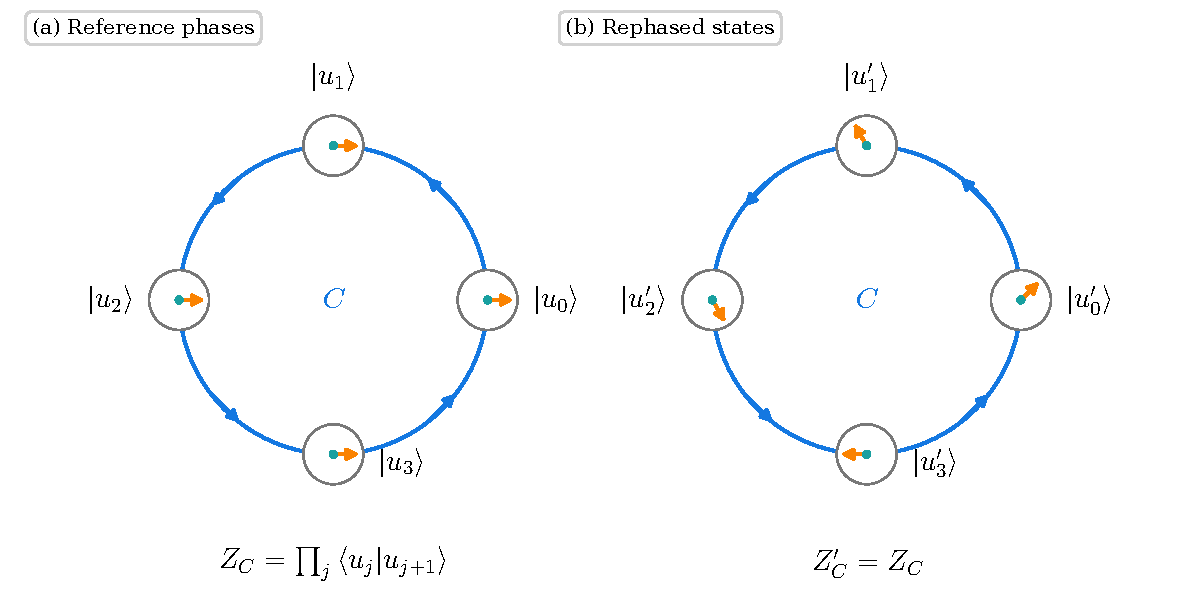
\includegraphics[width=0.8\textwidth]{figures_topo/C.1_phase_gauge.pdf}
    \caption{Two phase conventions along the same closed parameter path: (a) original representatives and (b) locally rephased representatives.}
    \label{fig:phase_gauge_appendix}
\end{figure}

The Berry phase describes the geometry of the electronic states along a chosen loop.
Here, following the loop means comparing stationary states at successive wave vectors;
we do not need to prescribe an actual time evolution of the electron.
Changing the arbitrary phase of each state leaves the closed-loop result unchanged,
whereas a smooth change of the hamiltonian or the loop can change $\mathrm{e}^{\mathrm{i}\gamma_n(C)}$ continuously,
provided the band remains non-degenerate along the loop.
The phase $\gamma_n(C)$ is not generally restricted to $0$ or $\mathrm{\pi}$.
The two-dimensional $\mathbb{Z}_2$ index requires additional structure, which comes from time-reversal symmetry and the full selected band subspace.

\subsection{From the Berry connection to the Berry curvature}
\label{subsec:berry_curvature_appendix}

The closed-loop phase compares states around a finite path.
We now ask how to describe this geometric information locally over a surface.
For a smooth non-degenerate band, we define the Berry curvature through the antisymmetric derivatives of the connection~\cite{xiao2010berry}:

\begin{equation}
\begin{aligned}
    \mathcal{F}_{n,ij}
    &\coloneqq\partial_{k_i}\mathcal{A}_{n,j}
    -\partial_{k_j}\mathcal{A}_{n,i} \\
    &=\mathrm{i}\left[
    \braket{\partial_{k_i}u_{n\vec{k}}|\partial_{k_j}u_{n\vec{k}}}
    -\braket{\partial_{k_j}u_{n\vec{k}}|\partial_{k_i}u_{n\vec{k}}}
    \right]
\end{aligned}
\label{abelian_berry_curvature_appendix}
\end{equation}

here, $\ket{\partial_{k_i}u_{n\vec{k}}}$ denotes $\partial_{k_i}\ket{u_{n\vec{k}}}$.
Under a smooth gauge transformation, the additional mixed derivatives of $\varphi_n$ cancel, giving $\mathcal{F}'_{n,ij}=\mathcal{F}_{n,ij}$.
Thus the single-band curvature is gauge invariant even though the connection depends on the gauge.
For an oriented surface $S$ in the $(k_x,k_y)$ plane, Stokes' theorem gives:

\begin{equation}
    \gamma_n(\partial S)
    =\oint_{\partial S}\vec{\mathcal{A}}_n\cdot\dif\vec{k}
    =\int_S\mathcal{F}_{n,xy}\dif k_x\dif k_y
    \qquad (\mathrm{mod}\ 2\mathrm{\pi})
\label{berry_curvature_stokes_appendix}
\end{equation}

This expression assumes that the band remains non-degenerate on the surface and that a smooth gauge is available over it.
The surface orientation fixes the boundary orientation.
For a sufficiently small loop, the curvature consequently gives the geometric phase per oriented area.
A loop winding around the periodically identified Brillouin zone need not bound such a surface within that zone;
equation~\eqref{berry_phase_closed_path_topology} still defines its phase, but the surface expression requires this additional check.

\subsection{The curvature in different dimensions}

In three-dimensional parameter space, we can express the same curvature as a vector:

\begin{equation}
\left\{\begin{aligned}
    \vec{\Omega}_n&=\nabla_{\vec{k}}\times\vec{\mathcal{A}}_n \\
    \Omega_{n,x}&=\mathcal{F}_{n,yz} \\
    \Omega_{n,y}&=\mathcal{F}_{n,zx}=-\mathcal{F}_{n,xz} \\
    \Omega_{n,z}&=\mathcal{F}_{n,xy}
\end{aligned}\right.
\label{berry_curvature_vector_appendix}
\end{equation}

Equivalently, $\Omega_{n,i}=\frac{1}{2}\sum_{j,l}\varepsilon_{ijl}\mathcal{F}_{n,jl}$,
where $\varepsilon_{ijl}$ is the Levi-Civita symbol in a right-handed coordinate system.
In two dimensions, $\mathcal{F}_{n,xy}$ is the perpendicular curvature component.
The relation resembles $\vec{B}=\nabla_{\vec{r}}\times\vec{A}_\mathrm{EM}$ in electrodynamics.
The connection plays the role of a vector potential, while the curvature plays the role of its field strength.
Adding a gradient changes the potential but leaves its curl unchanged.
Here, the field describes the electronic states in parameter space; the parameter space itself can be flat~\cite{xiao2010berry}.

For an arbitrary number of parameters, differential forms express the line and surface elements directly~\cite{hassani2013mathematical,nakahara2018geometry}.
Denoting the corresponding one-form and two-form by $\mathcal{A}_n$ and $\mathcal{F}_n$, we write:

\begin{equation}
\left\{\begin{aligned}
    \mathcal{A}_n&=\sum_i\mathcal{A}_{n,i}\dif k_i \\
    \mathcal{F}_n&=\dif\mathcal{A}_n
    =\sum_{i<j}\mathcal{F}_{n,ij}\dif k_i\wedge\dif k_j
\end{aligned}\right.
\label{berry_differential_forms_appendix}
\end{equation}

here, $\dif$ acting on a form denotes the exterior derivative.
The wedge product represents an oriented area element, with
$\dif k_i\wedge\dif k_j=-\dif k_j\wedge\dif k_i$ and $\dif k_i\wedge\dif k_i=0$.
These forms collect the same components used above;
integrating the one-form along a boundary or the two-form over its surface gives equation~\eqref{berry_curvature_stokes_appendix}.

\subsection{The curvature from a projector}

The phase freedom in equation~\eqref{bloch_phase_freedom_topology} leaves the single-state projector
$\hat{\mathcal{P}}_n=\ket{u_{n\vec{k}}}\bra{u_{n\vec{k}}}$ unchanged.
This projector alone consequently cannot determine the gauge-dependent connection.
We differentiate $\hat{\mathcal{P}}_n^2=\hat{\mathcal{P}}_n$ and use its constant unit trace to obtain:

\begin{equation}
\left\{\begin{aligned}
    \operatorname{Tr}\!\left[\hat{\mathcal{P}}_n\partial_{k_i}\hat{\mathcal{P}}_n\right]
    &=\frac{1}{2}\partial_{k_i}\operatorname{Tr}\hat{\mathcal{P}}_n^2=0 \\
    \mathcal{F}_{n,ij}
    &=\mathrm{i}\operatorname{Tr}\!\left[
    \hat{\mathcal{P}}_n[\partial_{k_i}\hat{\mathcal{P}}_n,\partial_{k_j}\hat{\mathcal{P}}_n]\right]
\end{aligned}\right.
\label{projector_berry_curvature_appendix}
\end{equation}

here, the trace is over the state space.
Substituting the differentiated ket-bra product into the second line, we recover equation~\eqref{abelian_berry_curvature_appendix}.
The projector therefore determines the curvature, while a connection additionally requires a choice of phase.

\subsection{A two-component example}
\label{subsec:berry_two_component_example_appendix}

We now apply these definitions to two orthonormal basis states $\ket{\uparrow}$ and $\ket{\downarrow}$.
We keep this basis fixed throughout the calculation.
For angular parameters $\theta$ and $\varphi$, we introduce the normalized state and hamiltonian:

\begin{equation}
\left\{\begin{aligned}
    \ket{v(\theta,\varphi)}
    &=\cos\frac{\theta}{2}\ket{\uparrow}
    +\mathrm{e}^{\mathrm{i}\varphi}\sin\frac{\theta}{2}\ket{\downarrow} \\
    \hat{h}(\theta,\varphi)
    &=\frac{\Delta}{2}\left[\hat{I}-2\ket{v(\theta,\varphi)}\bra{v(\theta,\varphi)}\right],
    \qquad \Delta>0
\end{aligned}\right.
\label{two_component_berry_state_appendix}
\end{equation}

The state $\ket{v}$ has energy $-\Delta/2$, while its orthogonal partner has energy $\Delta/2$.
The level separation therefore stays finite as the parameters change.
The angles specify this illustrative hamiltonian; they are independent of the crystal wave vectors used in the thesis calculations.
We evaluate the two derivatives and obtain:

\begin{equation}
\left\{\begin{aligned}
    \bra{v}\partial_\theta\ket{v}
    &=-\frac{1}{2}\cos\frac{\theta}{2}\sin\frac{\theta}{2}
    +\frac{1}{2}\sin\frac{\theta}{2}\cos\frac{\theta}{2}=0 \\
    \bra{v}\partial_\varphi\ket{v}
    &=\mathrm{i}\sin^2\frac{\theta}{2} \\
    \mathcal{A}_\theta&=0 \\
    \mathcal{A}_\varphi&=-\sin^2\frac{\theta}{2} \\
    \mathcal{F}_{\theta\varphi}
    &=\partial_\theta\mathcal{A}_\varphi-\partial_\varphi\mathcal{A}_\theta
    =-\frac{1}{2}\sin\theta
\end{aligned}\right.
\label{two_component_berry_derivatives_appendix}
\end{equation}

here, $\mathcal{A}_\varphi$ is the coefficient of $\dif\varphi$ in the connection integral.
For a loop at fixed $\theta=\theta_0$, traversed with $\varphi$ increasing from $0$ to $2\mathrm{\pi}$, we obtain:

\begin{equation}
    \gamma(C)
    =\int_0^{2\mathrm{\pi}}\mathcal{A}_\varphi(\theta_0)\dif\varphi
    =-2\mathrm{\pi}\sin^2\frac{\theta_0}{2}
    =-\mathrm{\pi}(1-\cos\theta_0)
    \qquad (\mathrm{mod}\ 2\mathrm{\pi})
\label{two_component_berry_phase_appendix}
\end{equation}

Integrating $\mathcal{F}_{\theta\varphi}$ over the cap $0\leq\theta\leq\theta_0<\mathrm{\pi}$, we recover the same result.
The chosen state is smooth over this cap; at the south pole $\theta=\mathrm{\pi}$, we must choose a different phase convention to remove its dependence on $\varphi$.
At $\theta_0=\mathrm{\pi}/2$, the phase is $-\mathrm{\pi}$, although the state representative returns to itself after a full turn.
Its parallel-transported representative instead returns with the factor $\mathrm{e}^{-\mathrm{i}\mathrm{\pi}}=-1$.
The example therefore connects the local connection and curvature to the closed-loop phase.
It also shows why a geometric phase can vary continuously with the path while the two levels remain separated.

We now represent the same example geometrically.
For the state in equation~\eqref{two_component_berry_state_appendix}, the expectation values of the Pauli operators define a unit vector:

\begin{equation}
\left\{\begin{aligned}
    n_i&=\bra{v}\hat{\sigma}_i\ket{v},\qquad i=x,y,z \\
    \vec{n}&=(\sin\theta\cos\varphi,\sin\theta\sin\varphi,\cos\theta)
\end{aligned}\right.
\label{two_component_state_sphere_appendix}
\end{equation}

here, $\hat{\sigma}_i$ are the Pauli operators in the fixed basis $\ket{\uparrow}$ and $\ket{\downarrow}$.
The vector $\vec{n}$ specifies a point on the unit sphere, often called the Bloch sphere.
Multiplying $\ket{v}$ by an overall phase leaves all three expectation values unchanged,
so one point represents a normalized state up to this phase freedom.
This sphere describes the two-component state; its coordinates are not the crystal wave vector or the real-space position of an electron.

For a second path, we choose $\theta_0=\mathrm{\pi}/3$, as shown in figure~\ref{fig:geometric_phase_appendix}(a).
The blue arrows show the direction of increasing $\varphi$ along the boundary of the shaded northern cap.
We relate the solid angle of this cap to the geometric phase through:

\begin{equation}
    \Omega_S=2\mathrm{\pi}(1-\cos\theta_0)=\mathrm{\pi},
    \qquad \gamma(C)=-\frac{\Omega_S}{2}=-\frac{\mathrm{\pi}}{2}
    \qquad (\mathrm{mod}\ 2\mathrm{\pi})
\label{two_component_solid_angle_appendix}
\end{equation}

Since the sphere has unit radius, this solid angle is also the surface area of the shaded cap.
Along this path, the chosen representative gives $\gamma(\varphi)=-\varphi\sin^2(\theta_0/2)$.
The factor $\mathrm{e}^{\mathrm{i}\gamma(\varphi)}$ therefore moves clockwise from $1$ to $-\mathrm{i}$ in the complex plane, as shown in panel (b).
Although $\ket{v(\theta_0,2\mathrm{\pi})}=\ket{v(\theta_0,0)}$, the parallel-transported representative
$\ket{\bar{v}(\varphi)}=\mathrm{e}^{\mathrm{i}\gamma(\varphi)}\ket{v(\theta_0,\varphi)}$
returns with $\ket{\bar{v}(2\mathrm{\pi})}=-\mathrm{i}\ket{\bar{v}(0)}$.
The path thus closes on the state sphere while retaining the phase mismatch described earlier.

\begin{figure}[htbp]
    \centering
    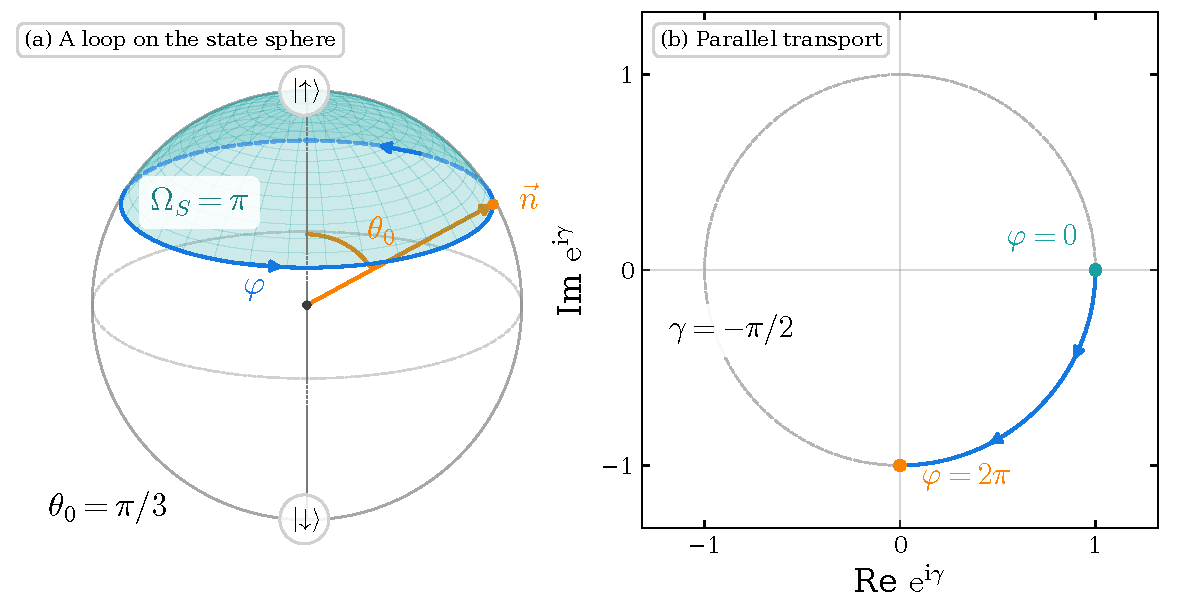
\includegraphics[width=0.8\textwidth]{figures_topo/C.2_geometric_phase.pdf}
    \caption{Geometric phase for $\theta_0=\mathrm{\pi}/3$: (a) the closed path on the state sphere and (b) the corresponding phase factor during parallel transport.}
    \label{fig:geometric_phase_appendix}
\end{figure}

\subsection{A connection to transverse transport}

The curvature also enters the motion of electrons under an external field.
We consider a wave packet in an isolated band under a weak electric field and zero magnetic field.
Its equations of motion read~\cite{sundaram1999wave,xiao2010berry}:

\begin{equation}
\left\{\begin{aligned}
    \hbar\dot{\vec{k}}&=-e\vec{E} \\
    \dot{\vec{r}}&=\frac{1}{\hbar}\nabla_{\vec{k}}E_{n\vec{k}}
    -\dot{\vec{k}}\times\vec{\Omega}_n
\end{aligned}\right.
\label{berry_anomalous_velocity_appendix}
\end{equation}

here, the electron charge is $-e$, with $e>0$.
The curvature term produces a velocity perpendicular to the electric field.
In two dimensions, we sum its charge-current contribution over occupied states and obtain:

\begin{equation}
    \sigma_{xy}^{\mathrm{int}}
    =-\frac{e^2}{\hbar}\sum_n\int_\mathrm{BZ}
    \frac{\dif^2k}{(2\mathrm{\pi})^2}\,
    f_{n\vec{k}}\Omega_{n,z}(\vec{k}\,)
\label{intrinsic_hall_curvature_appendix}
\end{equation}

here, $j_x=\sigma_{xy}^{\mathrm{int}}E_y$ fixes the sign convention,
and $f_{n\vec{k}}$ is the Fermi--Dirac occupation.
This is the intrinsic Hall contribution~\cite{nagaosa2010anomalous}; the ordinary Hall effect also involves the Lorentz force from a real magnetic field.
For an isolated band, the integrated curvature defines a Chern number.
For a band insulator at zero temperature, the Hall expression then reduces to~\cite{thouless1982quantized}:

\begin{equation}
    C_n=\frac{1}{2\mathrm{\pi}}\int_\mathrm{BZ}\Omega_{n,z}\dif^2k\in\mathbb{Z},
    \qquad \sigma_{xy}^{\mathrm{int}}=-\frac{e^2}{h}\sum_{n\,\mathrm{filled}}C_n
\label{chern_hall_relation_appendix}
\end{equation}

The integer counts the winding of phase transformations joining local gauges over the Brillouin zone.
During a smooth deformation, this integer can change only when the band loses its isolation.
For a band insulator with broken time-reversal symmetry, this relation describes the quantized anomalous Hall response.
With a magnetic field, the corresponding analysis uses magnetic bands.
Time-reversal-related states instead cancel their contributions to the intrinsic charge Hall conductivity.
They can still contribute to a spin Hall response, whose matrix elements involve the spin-current operator;
with spin-orbit coupling, this is not generally the difference of two independent spin-channel curvatures.
These examples explain the physical role of the curvature~\cite{xiao2010berry}.
The time-reversal invariant $\mathbb{Z}_2$ index used in this thesis requires the full band subspace, to which we now return.

\subsection{From an individual band to a band subspace}

So far, we have followed a single band separately from the other bands along the path.
We now consider spinful time-reversal-symmetric systems, where degeneracies also enter the problem.
Within a degenerate group, the hamiltonian alone does not select a unique state to follow.
Different choices can mix these states, rather than merely change their individual phases.
The degenerate subspace alone therefore does not fix an individual-band Berry phase.
We return to the projector in equation~\eqref{band_subspace_projector_topology}.

Within its $2N_\mathrm{p}$-dimensional subspace, we may choose a different orthonormal basis:

\begin{equation}
\left\{\begin{aligned}
    \ket{u'_{a\vec{k}}}
    &=\sum_{n=1}^{2N_\mathrm{p}}
    \ket{u_{n\vec{k}}}U_{na}(\vec{k}\,) \\
    U^\dagger(\vec{k}\,)U(\vec{k}\,)&=I \\
    \sum_{a=1}^{2N_\mathrm{p}}\ket{u'_{a\vec{k}}}\bra{u'_{a\vec{k}}}
    &=\hat{\mathcal{P}}(\vec{k}\,)
\end{aligned}\right.
\label{band_subspace_basis_transformation_topology}
\end{equation}

here, $U(\vec{k}\,)$ is a unitary matrix and $I$ is the identity matrix within the selected subspace.
When the transformation mixes states of different energies, the transformed basis need not diagonalize the hamiltonian.
Nevertheless, both bases span the same subspace and define the same projector.
This extends the phase freedom of an individual state to the choice of basis within a group of states.

We illustrate this freedom with a two-dimensional plane in a real three-dimensional inner-product space in figure~\ref{fig:subspace_basis_appendix}.
The blue vectors $\ket{1}$ and $\ket{2}$ form one orthonormal basis for the shaded plane.
Rotating both vectors through the same angle $\alpha=\mathrm{\pi}/5$ within the plane gives the orange basis $\ket{1'}$ and $\ket{2'}$.
This real rotation is a special case of a unitary transformation.
Both bases span the same plane and define the same projector $\hat{\mathcal{P}}$.
We keep the test state $\ket{\psi}$ fixed when we change the basis.
Consequently, this basis rotation leaves the projection $\hat{\mathcal{P}}\ket{\psi}$ of a test state outside the plane unchanged.
The plane represents a subspace of states,
and the actual Bloch states belong to a complex Hilbert space of general dimension.

\begin{figure}[htbp]
    \centering
    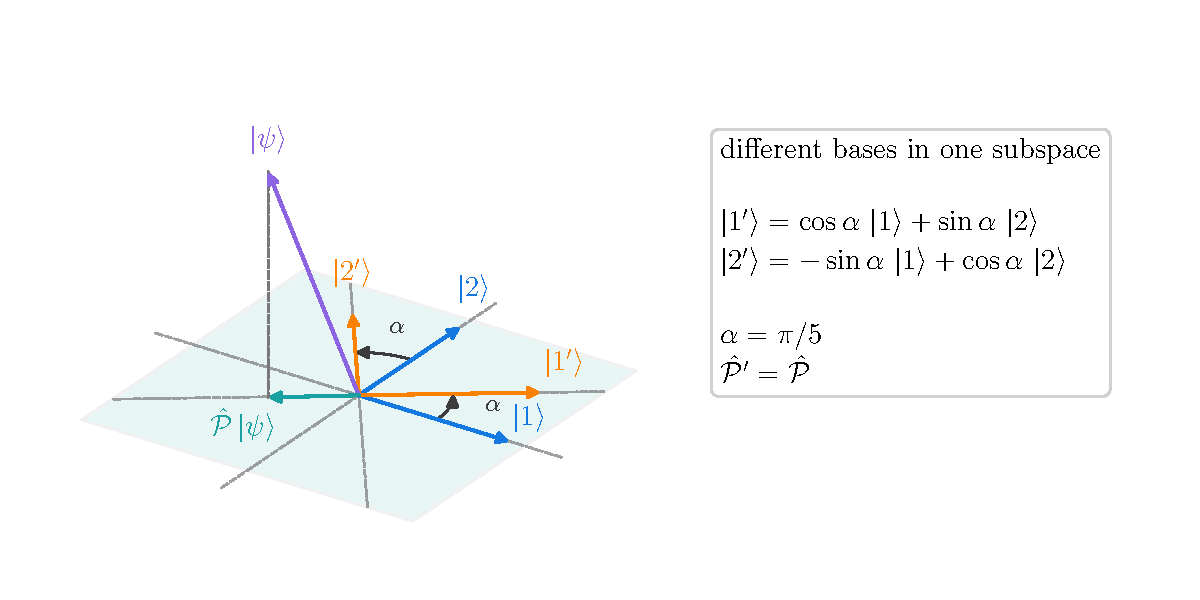
\includegraphics[width=0.8\textwidth]{figures_topo/C.3_subspace_basis.pdf}
    \caption{Two orthonormal bases spanning the same subspace, with the same projector and the same projection of $\ket{\psi}$.}
    \label{fig:subspace_basis_appendix}
\end{figure}

We now extend the single-state Berry connection to this basis.
We apply the derivative in equation~\eqref{berry_connection_topology} to each pair of basis states and obtain a matrix connection~\cite{wilczek1984appearance}:

\begin{equation}
\left\{\begin{aligned}
    [\vec{\mathcal{A}}(\vec{k}\,)]_{mn}
    &=\mathrm{i}\bra{u_{m\vec{k}}}\nabla_{\vec{k}}\ket{u_{n\vec{k}}} \\
    \vec{\mathcal{A}}\,'(\vec{k}\,)
    &=U^\dagger(\vec{k}\,)\vec{\mathcal{A}}(\vec{k}\,)U(\vec{k}\,)
    +\mathrm{i}\,U^\dagger(\vec{k}\,)\nabla_{\vec{k}}U(\vec{k}\,)
\end{aligned}\right.
\label{band_subspace_connection_topology}
\end{equation}

here, $m$ and $n$ run over the selected basis states.
We obtain the second relation by differentiating both the original basis and the matrix $U(\vec{k}\,)$.
For a single state, it reduces to equation~\eqref{berry_connection_gauge_transformation_topology}.
The off-diagonal elements describe the mixing of basis states as $\vec{k}$ changes.
The corresponding curvature is also a matrix:

\begin{equation}
\left\{\begin{aligned}
    \mathcal{F}_{ij}
    &=\partial_{k_i}\mathcal{A}_j-\partial_{k_j}\mathcal{A}_i
    -\mathrm{i}[\mathcal{A}_i,\mathcal{A}_j] \\
    \mathcal{F}'_{ij}&=U^\dagger\mathcal{F}_{ij}U
\end{aligned}\right.
\label{nonabelian_berry_curvature_appendix}
\end{equation}

The commutator accounts for the order of the matrix operations.
This is the non-Abelian generalization of equation~\eqref{abelian_berry_curvature_appendix}~\cite{wilczek1984appearance,xiao2010berry}.
The matrix curvature transforms covariantly under a change of basis; its trace is gauge invariant.
The same differential-form notation applies with matrix-valued coefficients~\cite{hassani2013mathematical}, and gives
$\mathcal{F}=\dif\mathcal{A}-\mathrm{i}\mathcal{A}\wedge\mathcal{A}$.
The ordered matrix products in the wedge term give the commutator in equation~\eqref{nonabelian_berry_curvature_appendix}.
Consequently, assigning independent single-band phases to arbitrary members of a degenerate pair does not characterize the whole subspace.
We now ask whether we can join these local bases over the whole Brillouin zone
while respecting time-reversal pairing.
This is a constraint on the full subspace, beyond the phase accumulated around one loop.
Using inversion symmetry, we evaluate the corresponding $\mathbb{Z}_2$ index from parity eigenvalues in chapter~\ref{cha:fundamentals_c}.
We first establish how time reversal acts on the same states.

\newpage
\section{Spinor states and time reversal}
\label{sec:spinors_time_reversal_appendix}

Equation~\eqref{KS_spinor_equation_method} describes the full electronic spinor.
Using the Bloch representation in equation~\eqref{bloch_hamiltonian_topology},
we now express the corresponding cell-periodic state as:

\begin{equation}
    \ket{u_{n\vec{k}}}
    =\ket{u_{n\vec{k},\uparrow}}\otimes\ket{\uparrow}
    +\ket{u_{n\vec{k},\downarrow}}\otimes\ket{\downarrow}
\label{cell_periodic_spinor_topology}
\end{equation}

here, the two spatial components form one spinor state.
Spin-orbit coupling can mix these components, so spin is not generally a conserved band label~\cite{bihlmayer2022rashba}.
The time-reversal classification, however, remains applicable when the hamiltonian preserves time-reversal symmetry.

For spin-$1/2$ electrons, we choose the time-reversal operator as:

\begin{equation}
\left\{\begin{aligned}
    \hat{\Theta}&=\mathrm{i}\hat{\sigma}_y\hat{K} \\
    \hat{\Theta}^2&=-\hat{I} \\
    \hat{\Theta}\hat{h}(\vec{k}\,)\hat{\Theta}^{-1}
    &=\hat{h}(-\vec{k}\,)
\end{aligned}\right.
\label{spinful_time_reversal_topology}
\end{equation}

here, $\hat{\sigma}_y$ is the Pauli operator in the chosen spin basis,
$\hat{K}$ takes the complex conjugate in the position and spin representation,
and $\hat{I}$ is the identity operator.
The last relation states the symmetry condition on the hamiltonian.
It applies to the non-magnetic spinful problem considered here;
spin-orbit coupling alone does not break time-reversal symmetry.

Physically, time reversal reverses both the momentum and the spin.
The complex-conjugation operation also conjugates the coefficients of a linear combination:

\begin{equation}
    \hat{\Theta}\bigl(c_a\ket{a}+c_b\ket{b}\bigr)
    =c_a^*\hat{\Theta}\ket{a}+c_b^*\hat{\Theta}\ket{b}
\label{time_reversal_antilinearity_topology}
\end{equation}

here, $c_a$ and $c_b$ are complex coefficients.
We call this property antilinearity.
In the chosen spin basis, the convention in equation~\eqref{spinful_time_reversal_topology} gives
$\hat{\Theta}\ket{\uparrow}=-\ket{\downarrow}$ and
$\hat{\Theta}\ket{\downarrow}=\ket{\uparrow}$.
Applying time reversal twice therefore returns either spin state with a minus sign,
which explains $\hat{\Theta}^2=-\hat{I}$.
We therefore distinguish the two components of one spinor from its time-reversed partner, which is another complete state.

The operator $\hat{\Theta}$ preserves norms while conjugating inner products, and is therefore antiunitary.
For any two states, it satisfies
$\braket{\hat{\Theta}a|\hat{\Theta}b}=\braket{b|a}$.
To apply this relation at a time-reversal invariant momentum (TRIM), we use a full Bloch state $\ket{\psi}$.
At such a point, the reversed wave vector differs from the original by a reciprocal-lattice vector,
so both states have the same phases under lattice translations.
Taking $\ket{a}=\ket{\psi}$ and $\ket{b}=\hat{\Theta}\ket{\psi}$, we obtain:

\begin{equation}
    \braket{\hat{\Theta}\psi|\psi}
    =\braket{\hat{\Theta}\psi|\hat{\Theta}^2\psi}
    =-\braket{\hat{\Theta}\psi|\psi}
\label{kramers_orthogonality_topology}
\end{equation}

Consequently, $\braket{\hat{\Theta}\psi|\psi}=0$.
Time-reversal symmetry also imposes $\hat{h}\hat{\Theta}=\hat{\Theta}\hat{h}$ on the full hamiltonian.
If $\hat{h}\ket{\psi}=E\ket{\psi}$, its partner therefore satisfies:

\begin{equation}
    \hat{h}\hat{\Theta}\ket{\psi}
    =\hat{\Theta}\hat{h}\ket{\psi}
    =E\hat{\Theta}\ket{\psi}
\label{kramers_equal_energy_topology}
\end{equation}

here, the energy $E$ is real because $\hat{h}$ is Hermitian.
At a wave vector equivalent to its negative, $\ket{\psi}$ and $\hat{\Theta}\ket{\psi}$
therefore represent orthogonal states with the same energy and wave vector.
These states form a Kramers pair~\cite{dresselhaus2008group}.
Removing the same Bloch factor from both states preserves their orthogonality,
so we also obtain two orthogonal cell-periodic states at this representative wave vector.
At a general wave vector, time reversal instead relates a state at $\vec{k}$ to an equal-energy state at $-\vec{k}$.

\cleardoublepage
\chapter{Source code and data analysis}
\label{cha:appendix_code}

The program code developed for this thesis is available through the following \texttt{GitHub} repositories.
It supports data analysis, data fitting,
derived physical-property calculations, and figure generation.

\hyperref[cha:project_bilayers]{Chapter~\ref*{cha:project_bilayers}: \nameref*{cha:project_bilayers}}
\cite{niu2024electronic}

\quad\href{https://github.com/Photonico/Graphene-BC_20230622}
{\texttt{https://github.com/Photonico/Graphene-BC\_20230622}}

\hyperref[cha:project_boron]{Chapter~\ref*{cha:project_boron}: \nameref*{cha:project_boron}}
\cite{niu2026superconductivity}

\quad\href{https://github.com/Photonico/o-B14_20241024}
{\texttt{https://github.com/Photonico/o-B14\_20241024}}

\hyperref[cha:project_beryllene]{Chapter~\ref*{cha:project_beryllene}: \nameref*{cha:project_beryllene}}
\cite{niu2026draftemergent}

\quad\href{https://github.com/Photonico/H-Beryllene_20250718}
{\texttt{https://github.com/Photonico/H-Beryllene\_20250718}}

The thesis source files and related materials:

\quad\href{https://github.com/Photonico/PhD_thesis_20251216}
{\texttt{https://github.com/Photonico/PhD\_thesis\_20251216}}

Each chapter repository contains the scripts and \texttt{Jupyter} notebooks used for the corresponding chapter.
The main reusable analysis code is stored in a top-level \texttt{vmatplot} directory within each project repository.
These local versions share the same code base but reflect different stages of development.
Later repositories contain newer functionality and refinements.
The \texttt{Jupyter} notebooks provide complete usage examples for the corresponding analyses.

The candidate used \texttt{vmatplot} to process first-principles calculation data,
analyse band structures, total and projected densities of states, dielectric functions, phonon dispersions, AIMD trajectories, and convergence tests, fit numerical data, and generate figures.
In particular, the code calculates the derived optical properties from the dielectric function.

Unless otherwise stated in the repository,
the candidate releases the source code and related scripts under the MIT License.
This permissive licence allows reuse, modification, distribution, and adaptation of the code,
with retention of the original copyright and licence notice.


%%%% Bibliography
\cleardoublepage
\phantomsection
\printbibliography[title={References}]

\end{document}

% color references
% Names are case-sensitive; HTML values use xcolor's rounded conversion.
% xcolor base colors (19)
% red              #FF0000
% green            #00FF00
% blue             #0000FF
% brown            #BF8040
% lime             #BFFF00
% orange           #FF8000
% pink             #FFBFBF
% purple           #BF0040
% teal             #008080
% violet           #800080
% cyan             #00FFFF
% magenta          #FF00FF
% yellow           #FFFF00
% olive            #808000
% black            #000000
% darkgray         #404040
% gray             #808080
% lightgray        #BFBFBF
% white            #FFFFFF
%
% dvipsnames colors (68)
% GreenYellow      #D9FF4F
% Yellow           #FFFF00
% Goldenrod        #FFE529
% Dandelion        #FFB529
% Apricot          #FFAD7A
% Peach            #FF804D
% Melon            #FF8A80
% YellowOrange     #FF9400
% Orange           #FF6321
% BurntOrange      #FF7D00
% Bittersweet      #C20300
% RedOrange        #FF3B21
% Mahogany         #A60000
% Maroon           #AD0000
% BrickRed         #B80000
% Red              #FF0000
% OrangeRed        #FF0080
% RubineRed        #FF00DE
% WildStrawberry   #FF0A9C
% Salmon           #FF789E
% CarnationPink    #FF5EFF
% Magenta          #FF00FF
% VioletRed        #FF30FF
% Rhodamine        #FF2EFF
% Mulberry         #A314FA
% RedViolet        #9600A8
% Fuchsia          #7303EB
% Lavender         #FF85FF
% Thistle          #E069FF
% Orchid           #AD5CFF
% DarkOrchid       #9933CC
% Purple           #8C24FF
% Plum             #8000FF
% Violet           #361FFF
% RoyalPurple      #401AFF
% BlueViolet       #1A0DF5
% Periwinkle       #6E73FF
% CadetBlue        #616EC4
% CornflowerBlue   #59DEFF
% MidnightBlue     #007091
% NavyBlue         #0F75FF
% RoyalBlue        #0080FF
% Blue             #0000FF
% Cerulean         #0FE3FF
% Cyan             #00FFFF
% ProcessBlue      #0AFFFF
% SkyBlue          #61FFE0
% Turquoise        #26FFCC
% TealBlue         #1FFAA3
% Aquamarine       #2EFFB2
% BlueGreen        #26FFAB
% Emerald          #00FF80
% JungleGreen      #03FF7A
% SeaGreen         #4FFF80
% Green            #00FF00
% ForestGreen      #00E000
% PineGreen        #00BF29
% LimeGreen        #80FF00
% YellowGreen      #8FFF42
% SpringGreen      #BDFF3D
% OliveGreen       #009900
% RawSienna        #8C0000
% Sepia            #4D0000
% Brown            #660000
% Tan              #DB9470
% Gray             #808080
% Black            #000000
% White            #FFFFFF
